% C S O U N D   5   M A N U A L 
% The manual is produced from 3 sources: this header document for new features and users' guide;
% Kevin Conder's ACRM translated to LaTeX for Csound language reference documentation; 
% and autogenerated Doxygen LaTeX files for Csound API reference documentation. To produce the entire manual:
% 1. Run Doxygen in the csound5 directory. It will produce LaTeX output that includes the contents of this file,
%    as well as API documentation automatically generated from various Csound and CsoundVST header files.
% 2. This file \includes{} (almost) all the HTML files from the Kevin Conder "Alternative Csound Reference Manual",
%    which have been translated to LaTeX using the html2latex Perl script. (If you need to re-run this script,
%    you will need to search and replace in the translated .tex files to comment out the preambles, end document statements,
%    and other stuff. You can use the Bk ReplaceEm Windows program with the csound5/doc/manual/replacements.txt search and 
%    replace table. But, don't! Forget the Conder docbook files and maintain the tex files instead -- please!)
% 3. Doxygen will produce a doc/csound/latex/refman.tex file. Run pdflatex on this file to generate csound.pdf. You can
%    also run tex4ht on this file to produce an HTML form of the manual. Be sure to run in a mode that skips right on past
%    all the hundreds of LaTeX errors!
% 4. Steps 1 and 3 are automated in SConstruct with the generatePdf=1 option.
\documentclass[10pt,letterpaper,onecolumn]{scrbook}
\usepackage{tocloft}
\usepackage{stdclsdv}
\usepackage{comment}
\usepackage{vmargin}
\usepackage{t1enc}
\usepackage{fancyvrb}
\usepackage{url}
\usepackage{calc}
\usepackage{array}
\usepackage{scrpage2}
\usepackage[pdftex]{graphicx}
\usepackage{color}
\usepackage{listings}
\usepackage[latin1]{inputenc}
\usepackage[english]{babel}
\usepackage{doxygen}
\usepackage{supertabular}
\usepackage[pdftex,
            pagebackref=true,
            colorlinks=true,
            linkcolor=blue,
            pdfpagelabels,
            pdfstartpage=3
           ]{hyperref}
\pagestyle{scrheadings}
\makeindex
\definecolor{LstColor}{cmyk}{0.1,0.1,0,0.025} 
\setlength{\cftsecnumwidth}{4em}
\lstset{language=c++,basicstyle=\ttfamily\scriptsize,commentstyle=\ttfamily\scriptsize,tabsize=2,breaklines,backgroundcolor=\color{LstColor},fontadjust=true,fancyvrb=true,moredelim=[is][\textbf]{\\emph\{}{\}}}.
\setcounter{tocdepth}{1}
\begin{document}

\frontmatter

\pagenumbering{roman}

\title{Csound and CsoundVST \\ Reference Manual} 
\author{\emph{By} \\ \\Barry Vercoe \\ \\ Contributors \\ \\ \\ \emph{Edited by} \\ \\ John ffitch \\ \\ Jean Piche \\ \\ Peter Nix \\ \\ Richard Boulanger \\ \\ Rasmus Ekman \\ \\ David Boothe \\ \\ Kevin Conder \\ \\ Michael Gogins \\ \texttt{gogins@pipeline.com} \\ }

\maketitle

\tableofcontents[2]

\setcounter{secnumdepth}{-1}    

\chapter{Preface}

\emph{By Barry Vercoe}

Realizing music by digital computer involves synthesizing audio signals with discrete points or samples
representative of continuous waveforms. There are many ways to do this, each affording a different manner
of control. Direct synthesis generates waveforms by sampling a stored function representing a single cycle;
additive synthesis generates the many partials of a complex tone, each with its own loudness envelope;
subtractive synthesis begins with a complex tone and filters it. Non--linear synthesis uses frequency
modulation and waveshaping to give simple signals complex characteristics, while sampling and storage of a
natural sound allows it to be used at will.

Since comprehensive moment--by--moment specification of sound can be tedious, control is gained in two
ways: 1) from the instruments in an orchestra, and 2) from the events within a score. An orchestra is really a
computer program that can produce sound, while a score is a body of data which that program can react to.
Whether a rise-time characteristic is a fixed constant in an instrument, or a variable of each note in the score,
depends on how the user wants to control it.

The instruments in a Csound orchestra are defined in a simple syntax that invokes complex audio
processing routines. A score passed to this orchestra contains numerically coded pitch and control
information, in standard numeric score format. Although many users are content with this format, higher
level score processing languages are often convenient.

The programs making up the Csound system have a long history of development, beginning with the Music 4
program written at Bell Telephone Laboratories in the early 1960s by Max Mathews. That initiated the stored
table concept and much of the terminology that has since enabled computer music researchers to
communicate. Valuable additions were made at Princeton by the late Godfrey Winham in Music 4B; my own
Music 360 (1968) was very indebted to his work. With Music 11 (1973) I took a different tack: the two distinct
networks of control and audio signal processing stemmed from my intensive involvement in the preceding
years in hardware synthesizer concepts and design. This division has been retained in Csound.
Because it is written entirely in C, Csound is easily installed on any machine running Unix or C. At MIT it runs
on VAX/DECstations under Ultrix 4.2, on SUNs under OS 4.1, SGIs under 5.0, on IBM PCs under DOS 6.2 and
Windows 3.1, and on the AppleMacintosh under ThinkC 5.0. With this single language for defining the audio
signal processing, and portable audio formats like AIFF andWAV, users can move easily from machine to
machine.

The 1991 version added phase vocoder, FOF, and spectral data types. 1992 saw MIDI converter and control
units, enabling Csound to be run from MIDI score-files and external keyboards. In 1994 the sound analysis
programs (lpc, pvoc) were integrated into the main load module, enabling all Csound processing to be run
from a single executable, and Cscore could pass scores directly to the orchestra for iterative performance. The
1995 release introduced an expanded MIDI set with MIDI-based linseg, butterworth filters, granular
synthesis, and an improved spectral-based pitch tracker. Of special importance was the addition of run-time
event generating tools (Cscore and MIDI) allowing run-time sensing and response setups that enable
interactive composition and experiment. It appeared that real-time software synthesis was now showing
some real promise.

\chapter{Licenses}

\section{Csound and CsoundVST}

Csound is \copyright 1991--2003 by Barry Vercoe and John ffitch.

CsoundVST is \copyright 2001--2004 by Michael Gogins.

Csound and CsoundVST are free software; you can redistribute them and/or modify them under the terms of the GNU Lesser General Public License as published by the Free Software Foundation; either version 2.1 of the License, or (at your option) any later version.

Csound and CsoundVST are distributed in the hope that they will be useful, but WITHOUT ANY WARRANTY; without even the implied warranty of MERCHANTABILITY or FITNESS FOR A PARTICULAR PURPOSE.  See the GNU Lesser General Public License for more details.

You should have received a copy of the GNU Lesser General Public License along with Csound and CsoundVST; if not, write to the Free Software Foundation, Inc., 59 Temple Place, Suite 330, Boston, MA 02111-1307 USA.

\section{Manual}

Permission is granted to copy, distribute and/or modify this document under the terms of the
GNU Free Documentation License, Version 1.2 or any later version published by the Free Software
Foundation; with no Invariant Sections, no Front-Cover Texts, and no Back-Cover Texts. A copy
of this license is available in the \texttt{doc/manual/copying.txt} file.

This Csound language documentation in this manual is derived from Kevin Conder's \emph{Alternative Csound Reference Manual}, which in turn is derived from the \emph{Public Csound Reference Manual}.

Copyright \copyright 2003 by Kevin Conder for modifications made to the \emph{Public Csound Reference Manual}.

Copyright \copyright 2004 by Michael Gogins for modifications made to the \emph{Alternative Csound Reference Manual}.

This legal notice is from the \emph{Public Csound Reference Manual}:

\begin{quotation}
	The original Hypertext Edition of the MIT Csound Manual was prepared for the World Wide Web by Peter J. Nix of the Department
	of Music at the University of Leeds and Jean Pich� of the Facult� de musique de l'Universit� de
	Montr�al. A Print Edition, in Adobe Acrobat format, was then maintained by David M. Boothe.
	The editors fully acknowledge the rights of the authors of the original documentation and programs,
	as set out above, and further request that this notice appear wherever this material is held.
\end{quotation}

The Public Csound Reference Manual's last known network location was \url{http://www.
lakewoodsound.com/csound/hypertext/manual.htm}.

The Alternative Csound Reference Manual's network location, for both the Transparent and
Opaque copies, is \url{http://kevindumpscore.com/download.html#csound-manual}.

\section{Virtual Synthesis Technology}
Virtual Synthesis Technology (VST) PlugIn interface technology by Steinberg Soft- und Hardware GmbH. 

CsoundVST source code contains modified versions of source code files from the VST SDK distributed by Steinberg. \emph{These files are to be used only for building CsoundVST.} You are \emph{not} licensed to use these files for any other purpose. If you make a derived product based on CsoundVST or the modified VST source files herein, you \emph{must} apply to Steinberg for your own license to use the VST SDK.

\chapter{Acknowledgments}

Csound contains contributions from musicians, scientists, and programmers from around the world. They include (but are not limited to): 

\begin{itemize}
\item Allan Lee 
\item Andres Cabrera
\item Barry Vercoe
\item Bill Gardner 
\item Bill Verplank 
\item Dan Ellis 
\item David Macintyre 
\item Eli Breder 
\item Gabriel Maldonado  
\item Greg Sullivan 
\item Hans Mikelson 
\item Istvan Varga 
\item Jean Piche 
\item John ffitch 
\item John Ramsdell 
\item Marc Resibois 
\item Mark Dolson 
\item Matt Ingalls 
\item Max Mathews 
\item Michael Casey 
\item Michael Clark 
\item Michael Gogins 
\item Mike Berry 
\item Paris Smaragdis 
\item Perry Cook 
\item Peter Neubacker 
\item Peter Nix 
\item Rasmus Ekman 
\item Richard Dobson 
\item Richard Karpen 
\item Rob Shaw 
\item Robin Whittle 
\item Sean Costello 
\item Steven Yi 
\item Tom Erbe 
\item Victor Lazzarini  
\item Ville Pulkki 
\end{itemize}

\chapter{To Do...}

This is a ``to do'' list, not necessarily complete, and in no particular order of priority or time, for Csound and CsoundVST:

\begin{enumerate}
\item See also the \texttt{To-fix-and-do} file in the \texttt{csound5} directory.
\item Create better examples, especially to demonstrate the use of Python and of VST plugins. One example should be a live performance instrument with a Python GUI that controls instrument parameters or algorithmic composition parameters in real time.
\item Complete the work of making Csound multi-instantiable.
\end{enumerate}

%\begin{comment}
\documentclass[10pt]{article}
\usepackage{fullpage, graphicx, url}
\setlength{\parskip}{1ex}
\setlength{\parindent}{0ex}
\title{Preface}
\begin{document}


\begin{tabular}{ccc}
The Alternative Csound Reference Manual & & \\
Previous & &Next

\end{tabular}

%\hline 
\end{comment}
\section{Preface}
\section{Preface to the Csound Manual}
Barry Vercoe

  by Barry L. Vercoe, MIT Media Lab 


  Realizing music by digital computer involves synthesizing audio signals with discrete points or samples representative of continuous waveforms. There are many ways to do this, each affording a different manner of control. Direct synthesis generates waveforms by sampling a stored function representing a single cycle; additive synthesis generates the many partials of a complex tone, each with its own loudness envelope; subtractive synthesis begins with a complex tone and filters it. Non-linear synthesis uses frequency modulation and waveshaping to give simple signals complex characteristics, while sampling and storage of a natural sound allows it to be used at will. 


  Since comprehensive moment-by-moment specification of sound can be tedious, control is gained in two ways: 1) from the instruments in an orchestra, and 2) from the events within a score. An orchestra is really a computer program that can produce sound, while a score is a body of data which that program can react to. Whether a rise-time characteristic is a fixed constant in an instrument, or a variable of each note in the score, depends on how the user wants to control it. 


  The instruments in a Csound orchestra (see ) are defined in a simple syntax that invokes complex audio processing routines. A score (see ) passed to this orchestra contains numerically coded pitch and control information, in standard numeric score format. Although many users are content with this format, higher level score processing languages are often convenient. 


  The programs making up the Csound system have a long history of development, beginning with the Music 4 program written at Bell Telephone Laboratories in the early 1960's by Max Mathews. That initiated the stored table concept and much of the terminology that has since enabled computer music researchers to communicate. Valuable additions were made at Princeton by the late Godfrey Winham in Music 4B; my own Music 360 (1968) was very indebted to his work. With Music 11 (1973) I took a different tack: the two distinct networks of control and audio signal processing stemmed from my intensive involvement in the preceding years in hardware synthesizer concepts and design. This division has been retained in Csound. 


  Because it is written entirely in C, Csound is easily installed on any machine running Unix or C. At MIT it runs on VAX/DECstations under Ultrix 4.2, on SUNs under OS 4.1, SGI's under 5.0, on IBM PC's under DOS 6.2 and Windows 3.1, and on the Apple Macintosh under ThinkC 5.0. With this single language for defining the audio signal processing, and portable audio formats like AIFF and WAV, users can move easily from machine to machine. 


  The 1991 version added phase vocoder, FOF, and spectral data types. 1992 saw MIDI converter and control units, enabling Csound to be run from MIDI score-files and external keyboards. In 1994 the sound analysis programs (lpc, pvoc) were integrated into the main load module, enabling all Csound processing to be run from a single executable, and Cscore could pass scores directly to the orchestra for iterative performance. The 1995 release introduced an expanded MIDI set with MIDI-based linseg, butterworth filters, granular synthesis, and an improved spectral-based pitch tracker. Of special importance was the addition of run-time event generating tools (Cscore and MIDI) allowing run-time sensing and response setups that enable interactive composition and experiment. It appeared that real-time software synthesis was now showing some real promise. 
%\hline 


\begin{comment}
\begin{tabular}{lcr}
Previous &Home &Next \\
The Alternative Csound Reference Manual &� &Copyright Notice

\end{tabular}


\end{document}
\end{comment}

%\begin{comment}
\documentclass[10pt]{article}
\usepackage{fullpage, graphicx, url}
\setlength{\parskip}{1ex}
\setlength{\parindent}{0ex}
\title{Acknowledgements}
\begin{document}


\begin{tabular}{ccc}
The Alternative Csound Reference Manual & & \\
Previous &Preface &Next

\end{tabular}

%\hline 
\end{comment}
\section{Acknowledgements}


  In addition to the core code developed by Barry L. Vercoe at M.I.T., a large part of the Csound code was modified, developed and extended by an independent group of programmers, composers and scientists. Copyright to this code is held by the respective authors: 


 \textbf{Table 1. Contributors}



\begin{tabular}{cccccccccccccccc}
Mike BerryRichard Karpen &Eli BrederVictor Lazzarini &Michael CaseyAllan Lee &Michael ClarkDavid Macintyre &Perry CookGabriel Maldonado &Sean CostelloMax Mathews &Richard DobsonHans Mikelson &Mark DolsonPeter Neub\"acker &Rasmus EkmanVille Pulkki &Dan EllisMarc Resibois &Tom ErbeParis Smaragdis &John ffitchRob Shaw &Bill GardnerGreg Sullivan &Matt IngallsBill Verplank &Istvan VargaRobin Whittle &Jean Pich\'ePeter Nix

\end{tabular}



  The official manual was compiled from the canonical Csound Manual sources maintained by John ffitch, Richard Boulanger, Jean Pich\'e, Peter Nix, and David M. Boothe. The Alternative Csound Reference Manual is maintained by Kevin Conder. 
%\hline 


\begin{comment}
\begin{tabular}{lcr}
Previous &Home &Next \\
Copyright Notice &Up &Why is this called the \emph{Alternative}
 Csound Reference Manual?

\end{tabular}


\end{document}
\end{comment}

%\begin{comment}
\documentclass[10pt]{article}
\usepackage{fullpage, graphicx, url}
\setlength{\parskip}{1ex}
\setlength{\parindent}{0ex}
\title{Copyright Notice}
\begin{document}


\begin{tabular}{ccc}
The Alternative Csound Reference Manual & & \\
Previous &Preface &Next

\end{tabular}

%\hline 
\end{comment}
\section{Copyright Notice}


  Copyright (c) 1986, 1992 by the Massachusetts Institute of Technology. All rights reserved. 


  Developed by \emph{Barry L. Vercoe}
 at the Experimental Music Studio, Media Laboratory, M.I.T., Cambridge, Massachusetts, with partial support from the System Development Foundation and from National Science Foundation Grant \# IRI-8704665. 


  Copyright (c) 2003 by Kevin Conder for modifications made to the Public Csound Reference Manual. 


  Permission is granted to copy, distribute and/or modify this document under the terms of the GNU Free Documentation License, Version 1.2 or any later version published by the Free Software Foundation; with no Invariant Sections, no Front-Cover Texts, and no Back-Cover Texts. A copy of this license is available in the examples sub-directory. 


  A legal notice from the Public Csound Reference Manual... ``The original Hypertext Edition of the MIT Csound Manual was prepared for the World Wide Web by \emph{Peter J. Nix}
 of the Department of Music at the University of Leeds and \emph{Jean Pich\'e}
 of the Facult\'e de musique de l'Universit\'e de Montr\'eal. A Print Edition, in Adobe Acrobat format, was then maintained by \emph{David M. Boothe}
. The editors fully acknowledge the rights of the authors of the original documentation and programs, as set out above, and further request that this notice appear wherever this material is held.''


  The Public Csound Reference Manual's last known network location was \url{http://www.lakewoodsound.com/csound/hypertext/manual.htm}. 


  The Alternative Csound Reference Manual's network location, for both the Transparent and Opaque copies, is \url{http://kevindumpscore.com/download.html}\#csound-manual. 
%\hline 


\begin{comment}
\begin{tabular}{lcr}
Previous &Home &Next \\
Preface &Up &Acknowledgements

\end{tabular}


\end{document}
\end{comment}

%\begin{comment}
\documentclass[10pt]{article}
\usepackage{fullpage, graphicx, url}
\setlength{\parskip}{1ex}
\setlength{\parindent}{0ex}
\title{Where is the documentation for the CsoundAV project?}
\begin{document}


\begin{tabular}{ccc}
The Alternative Csound Reference Manual & & \\
Previous &Preface &Next

\end{tabular}

%\hline 
\end{comment}
\section{Where is the documentation for the CsoundAV project?}


  The documentation for the CsoundAV project is located at \emph{\url{http://www.csounds.com/csoundav/index.html}}
. 
%\hline 


\begin{comment}
\begin{tabular}{lcr}
Previous &Home &Next \\
What is the scope of the Alternative Csound Reference Manual? &Up &Overview

\end{tabular}


\end{document}
\end{comment}

%\begin{comment}
\documentclass[10pt]{article}
\usepackage{fullpage, graphicx, url}
\setlength{\parskip}{1ex}
\setlength{\parindent}{0ex}
\title{Why is this called the Alternative Csound Reference Manual?}
\begin{document}


\begin{tabular}{ccc}
The Alternative Csound Reference Manual & & \\
Previous &Preface &Next

\end{tabular}

%\hline 
\end{comment}
\section{Why is this called the \emph{Alternative}
 Csound Reference Manual?}


  When I originally started my manual project, there was already an Official Csound Reference Manual (last known address: \emph{\url{http://www.lakewoodsound.com/csound/hypertext/manual.htm}}
). The Official manual was maintained by David M. Boothe. I found its layout confusing and I wanted to change it. But since it was maintained with a commercial word processing program, I couldn't. I could neither afford this program nor was it available for my main computing platform. 


  So I created an alternative to the Official Csound Reference Manual. I distributed my manual using the \emph{DocBook/SGML}
 format so that anyone on any platform could edit it with a text editor. This manual can also be produced with freely available programs. 


  David M. Boothe wasn't interested in maintaining my DocBook/SGML version of the manual. He was also concerned that people would confuse his project (the ``Official'' one) with mine. So out of respect for his wishes, I named my project the Alternative Csound Reference Manual. I made this decision so that nobody would confuse my project (the ``Alternative'' one) with his. 


  Written by Kevin Conder, October 2002. 
%\hline 


\begin{comment}
\begin{tabular}{lcr}
Previous &Home &Next \\
Acknowledgements &Up &What is the scope of the Alternative Csound Reference Manual?

\end{tabular}


\end{document}
\end{comment}

%\begin{comment}
\documentclass[10pt]{article}
\usepackage{fullpage, graphicx, url}
\setlength{\parskip}{1ex}
\setlength{\parindent}{0ex}
\title{What is the scope of the Alternative Csound Reference Manual?}
\begin{document}


\begin{tabular}{ccc}
The Alternative Csound Reference Manual & & \\
Previous &Preface &Next

\end{tabular}

%\hline 
\end{comment}
\section{What is the scope of the Alternative Csound Reference Manual?}


  While there are numerous Csound-related projects, this manual only covers the canonical Csound program. This program is maintained by John ffitch and is stored on the Bath University FTP server (\emph{\url{ftp://www.cs.bath.ac.uk/pub/dream/newest/}}
). I apologize that I can't maintain the documentation for other projects. I simply don't have the time and resources to do so. 


  Written by Kevin Conder, January 2003. 
%\hline 


\begin{comment}
\begin{tabular}{lcr}
Previous &Home &Next \\
Why is this called the \emph{Alternative}
 Csound Reference Manual? &Up &Where is the documentation for the CsoundAV project?

\end{tabular}


\end{document}
\end{comment}


\setcounter{secnumdepth}{2}    

\mainmatter

\pagenumbering{arabic}
\setcounter{page}{1}

\part{Csound User's Guide}

\chapter{Introduction}

\emph{By Michael Gogins}

Csound is a unit generator--based, user--programmable computer music system. It was originally written by Barry Vercoe at the Massachusetts Institute of Technology in 1984 as the first C language version of this type of software. Since then Csound has received numerous contributions from researchers, programmers, and musicians from around the world. 

Around 1991, John ffitch ported Csound to Microsoft DOS. Csound currently runs on many varieties of UNIX and Linux, Microsoft DOS and Windows, all versions of the Macintosh operating system including Mac OS X, and others.

There are newer computer music systems that have graphical patch editors (e.g. Max/MSP, PD, jMax, or Open Sound World), or that use more advanced techniques of software engineering (e.g. Nyquist or SuperCollider). Yet Csound still has the largest and most varied set of unit generators, is the best documented, runs on the most platforms, and is the easiest to extend. It is possible to compile Csound using double-precision arithmetic throughout for superior sound quality. In short, Csound must be considered one of the most powerful musical instruments ever created.

To make music with Csound:

\begin{enumerate}
\item Write an orchestra (\texttt{.orc} file) that creates instruments and signal processors by connecting unit generators (also called opcodes, in Csound-speak) using Csound's simple programming language.
\item Write a score (\texttt{.sco} file) that specifies a list of notes and other events to be rendered by the orchestra.
\item Run Csound to compile the orchestra and score, run the sorted and preprocessed score through the orchestra, and write digital audio out to a soundfile or sound card.
\end{enumerate}

CsoundVST is an extended version of Csound that adds a graphical user interface, C++ and Python APIs, Python scripting, a library of Python extension modules for algorithmic composition, a VST plugin interface, and a \emph{Mathematica} interface.

In addition to this ``canonical'' version of Csound and CsoundVST, there are other versions of Csound and other front ends for Csound, many of which can be found at \url{http://csounds.com}.

\section{Recent Developments}

In the time since Barry Vercoe wrote the original preface to this manual, printed above, many further contributions have been made to Csound. The current stable version of Csound is 4.23. Csound 5 is the next version, currently in late alpha or early beta status. CsoundVST is an extended version of both Csound 4 and Csound 5.

\section{New Features in Csound 5}

Csound 5 begins a major new version of Csound that includes the following new features:

\begin{itemize}

\item Now licensed under the GNU Lesser General Public License, an open source license.

\item A new, easier to manage build system using \texttt{scons}.

\item The use of widely--accepted open source libraries:

\begin{itemize}

\item libsndfile for soundfile input and output.

\item PortAudio with ASIO drivers for low-latency, real-time audio input and output.

\item FLTK for graphical widgets that can be programmed in orchestra code.

\item \emph{Will} use PortMidi for real-time MIDI input and output.

\end{itemize}

\item Simplified audio buffering system.

\item Status returns on all internal functions, including opcode functions.

\item MIDI interop opcodes, that enable the same instrument definitions to be used interchangeably for either live MIDI performance or off-line, score-driven performance.

\item Plugin opcodes are working and becoming more widely accepted. Many opcodes have been moved to plugins. Most new opcodes are plugins, including:

\begin{itemize}

\item SoundFont opcodes.

\item Python opcodes allowing Python code to execute in the orchestra header or in instrument code, at \texttt{i}-rate or \texttt{k}-rate.

\item Loris opcodes for time/frequency analysis and resynthesis.

\item Bus opcodes.

\item \texttt{vst4cs} VST plugin adapter opcodes.

\end{itemize}

\item The \texttt{OpcodeBase.hpp} header file for writing plugin opcodes in C++. This is based on the technique of static polymorphism via template inheritance.

\item The Csound API is becoming more widely used.

\end{itemize}

John ffitch plans to replace the handwritten parser with one written using a parser generator, which should make it more bug-free and perhaps more efficient.

John ffitch and I have plans for creating multiple instances of Csound in the same process, though we are only about halfway there.

\section{Features of CsoundVST}

CsoundVST is an extended version of Csound that runs both as a shared library (as a VST plugin or as an embedded synthesizer) and as a standalone program. Its main purposes are (a) to make it easier to extend Csound (e.g. the Loris plugin opcodes with their Python scripting), and (b) to streamline the actual use of Csound in composing, particularly for algorithmic composition, by integrating more tightly with other languages and other software.

\begin{itemize}

\item Variant version of the Csound ``C'' API, with score management facilities.

\item Extended C++ version of the Csound API, with score management facilities and function table access.

\item C++ library for algorithmic composition, based on my concept of music graphs.

\item Python wrappers for the Csound API and for music graphs.

\item Built-in Python interpreter. This enables one to embed orchestras and scores into Python code, and to write Csound pieces in Python, including both composition and synthesis.

\item Runs as a VST effect or VST plugin.

\begin{itemize}

\item Loads and saves \texttt{.csd} and \texttt{.py} files in presets and banks.

\item Starts, stops, and restarts.

\item Allows one to write Csound pieces in music notation and hear the results immediately.

\item Synchronizes with other tracks in the same host, including looping.

\end{itemize}

\item Runs as a standalone application.

\item Runs as a Python extension module. This enables one to write Csound pieces in any Python interpreter.

\item The Csound API is being extended to handle function tables and other internals of Csound.

\end{itemize}

\chapter{Csound Links}

Csound's ``home page'' is maintained by Richard Boulanger at \url{http://csounds.com}. 

The Csound source code is maintained by John ffitch at \url{http://www.sourceforge.net/projects/csound}. Precompiled packages for some platforms also can be downloaded from that site.

A Csound mailing list exists to discuss Csound. It is run by John ffitch of Bath University, UK. To have your name put on the mailing list send an empty message to \url{csound-subscribe@lists.bath.ac.uk}. Posts sent to \url{csound@lists.bath.ac.uk} go to all subscribed members of the list. 

Similarly, the CSOUND-DEV mailing list exists to discuss Csound development. For more information on this list, go to \url{http://eartha.mills.edu:8000/guest/listutil/CSOUND-DEV}. Posts sent to \url{csound-dev@eartha.mills.edu} go to all subscribed members of the list.

Suspected bugs in the code may be entered using the bug tracking system at \emph{\url{http://www.cs.bath.ac.uk/cgi-bin/csound}}. 

%\begin{comment}
\documentclass[10pt]{article}
\usepackage{fullpage, graphicx, url}
\setlength{\parskip}{1ex}
\setlength{\parindent}{0ex}
\title{The Csound Mailing List}
\begin{document}


\begin{tabular}{ccc}
The Alternative Csound Reference Manual & & \\
Previous &Introduction &Next

\end{tabular}

%\hline 
\end{comment}
\section{The Csound Mailing List}


  A Csound Mailing List exists to discuss Csound. It is run by John ffitch of Bath University, UK. 


  To have your name put on the mailing list send an empty message to: 


  \emph{csound-subscribe@lists.bath.ac.uk}
 


  Posts sent to  \emph{csound@lists.bath.ac.uk}
  go to all subscribed members of the list. 
\subsection*{Bug Reports}


  Suspected bugs in the code may be entered using the bug tracking system at \emph{\url{http://www.cs.bath.ac.uk/cgi-bin/csound}}
. 
%\hline 


\begin{comment}
\begin{tabular}{lcr}
Previous &Home &Next \\
How to Install Csound &Up &The Csound Command

\end{tabular}


\end{document}
\end{comment}


\chapter{Installing}

%\begin{comment}
\documentclass[10pt]{article}
\usepackage{fullpage, graphicx, url}
\setlength{\parskip}{1ex}
\setlength{\parindent}{0ex}
\title{How to Install Csound}
\begin{document}


\begin{tabular}{ccc}
The Alternative Csound Reference Manual & & \\
Previous &Introduction &Next

\end{tabular}

%\hline 
\end{comment}
\section{How to Install Csound}
\subsection*{Linux}


  Detailed instructions for installing and configuring Csound on a Linux system may be obtained from: 


  \emph{\url{http://www.csounds.com/secondprinting/cdroms/installing/linux/}}
 
\subsection*{Macintosh}


  Detailed instructions for installing and configuring Csound on Macintosh systems may be obtained from: 


  \emph{\url{http://www.csounds.com/installing/howtomacintosh/index.html}}
 
\subsection*{MS-DOS and Windows 95/NT}


  Detailed instructions for installing and configuring Csound on a MS-DOS or Windows 95/NT system may be obtained from: 


  \emph{\url{http://hem.passagen.se/rasmuse/PCinstal.htm}}
 
\subsection*{Windows 95/98/2000}


  Detailed instructions for installing and configuring Csound on a Windows 95, Windows 98, or Windows 2000 system may be obtained from: 


  \emph{\url{http://www.csounds.com/installing/howtowindows/index.html}}
 
\subsection*{Other Platforms}


  For information on availability of Csound for other platforms, see The Csound FrontPage: 


  \emph{\url{http://mitpress.mit.edu/e-books/csound/frontpage.html}}
 
%\hline 


\begin{comment}
\begin{tabular}{lcr}
Previous &Home &Next \\
Introduction &Up &The Csound Mailing List

\end{tabular}


\end{document}
\end{comment}


\section{Downloading}

Csound and CsoundVST source code is hosted at \url{http://www.sourceforge.net/projects/csound}. \linebreak Source and binary packages are available from the \texttt{files} link off that page.

%\begin{comment}
\documentclass[10pt]{article}
\usepackage{fullpage, graphicx, url}
\setlength{\parskip}{1ex}
\setlength{\parindent}{0ex}
\title{How to Install Csound}
\begin{document}


\begin{tabular}{ccc}
The Alternative Csound Reference Manual & & \\
Previous &Introduction &Next

\end{tabular}

%\hline 
\end{comment}
\section{How to Install Csound}
\subsection*{Linux}


  Detailed instructions for installing and configuring Csound on a Linux system may be obtained from: 


  \emph{\url{http://www.csounds.com/secondprinting/cdroms/installing/linux/}}
 
\subsection*{Macintosh}


  Detailed instructions for installing and configuring Csound on Macintosh systems may be obtained from: 


  \emph{\url{http://www.csounds.com/installing/howtomacintosh/index.html}}
 
\subsection*{MS-DOS and Windows 95/NT}


  Detailed instructions for installing and configuring Csound on a MS-DOS or Windows 95/NT system may be obtained from: 


  \emph{\url{http://hem.passagen.se/rasmuse/PCinstal.htm}}
 
\subsection*{Windows 95/98/2000}


  Detailed instructions for installing and configuring Csound on a Windows 95, Windows 98, or Windows 2000 system may be obtained from: 


  \emph{\url{http://www.csounds.com/installing/howtowindows/index.html}}
 
\subsection*{Other Platforms}


  For information on availability of Csound for other platforms, see The Csound FrontPage: 


  \emph{\url{http://mitpress.mit.edu/e-books/csound/frontpage.html}}
 
%\hline 


\begin{comment}
\begin{tabular}{lcr}
Previous &Home &Next \\
Introduction &Up &The Csound Mailing List

\end{tabular}


\end{document}
\end{comment}


\section{Configuration}

Once you have either unpacked a binary distribution, or built Csound from sources, you will need to configure Csound so that it will run properly on your system. 

\subsection{Csound}

On Windows, make sure the directory or directories (normally the \texttt{csound5} directory) containing the Csound executables directory and all the Csound plugin opcodes are also in your \texttt{PATH} variable, or else copy all the executable files to your Windows \texttt{system32} directory.

On Unix and Linux, either install the Csound program in one of the system \texttt{bin} directories, typically \texttt{/usr/local/bin}, and the Csound and plugin shared libraries in one of the system \texttt{lib} directories, typically \url{/usr/local/lib}; or make sure that the directory containing the Csound and plugin shared libraries is in your \texttt{LD\_LIBRARY\_PATH} environment variable. This variable may have a different name in different operating systems.

On all platforms, make sure the directory or directories containing Csound's plugin opcodes are in an \texttt{OPCODEDIR} environment variable.

\subsection{CsoundVST}

CsoundVST requires some additional configuration. On all platforms, CsoundVST requires that you have Python installed on your computer. The directory containing the \texttt{\_CsoundVST} shared library and the \texttt{CsoundVST.py} file must be in your \texttt{PYTHONPATH} environment variable, so that the Python runtime knows how to load these files.

\chapter{Using}

Assuming that you have installed and configured the software, Csound and CsoundVST can be operated in a variety of modes and configurations. The \texttt{.csd} and \texttt{.py} files in the \texttt{examples} demonstrate a few of these modes of operation. Some of these scores are simple, others are moderately complex. 

You may need to edit the \texttt{----opcode-lib} option in the Csound command in some of the  \texttt{.csd} and \texttt{.py} files to match your environment. Similarly, you may need to edit the SoundFont file paths in instrument definitions that use the \texttt{fluid} SoundFont 2 player opcode to match your environment.

\section{Real-Time Audio}

For real-time audio output, with or without MIDI control, you will probably want to tune the \texttt{kr} and \texttt{ksmps} orchestra statements, and the \texttt{-b} and \texttt{-B} command-line options, to give you the shortest possible latency that does not cause clicks or stutters in Csound's audio output. 

\subsection{Windows with ASIO}

On Windows, Csound is configured with the ASIO build of the PortAudio library. At this time, it is necessary to set both the \texttt{-B} and the \texttt{-b} command-line options to have the same value as the \texttt{ksmps} variable set in the orchestra file. For example, \texttt{sr = 44100}, \texttt{kr = 100}, \texttt{ksmps = 441}, \texttt{-b441} and \texttt{-B441} give a CD-equivalent audio sampling rate of 44,100 frames per second, a control sampling rate of 100 control samples per second with 441 audio sample frames per control sample, an audio output software buffer size of 441 sample frames, and an audio output device hardware buffer size of 441 sample frames, which yields an audio output latency of 10 milliseconds --- quite fast enough for reasonably expressive keyboard playing or other real-time instrumental performance. Even lower latencies are possible with smaller values of \texttt{-B}, \texttt{-b}, and \texttt{ksmps}, down to less than a millisecond on Windows XP.

If your sound card does not have an ASIO driver, you can still use Csound with ASIO by downloading and installing the \texttt{asio4all} adapter from \url{http://michael.tippach.bei.t-online.de/asio4all}.

\subsection{Linux with ALSA}

On Linux with ALSA, the audio output device should be selected using a special form of the \texttt{-odac} option, for example \texttt{-odac:plughw:0} for device 0. The \texttt{plughw} option translates Csound's audio output to the format expected by the sound card. With ALSA, latencies of a few milliseconds are possible, and expressive real-time instrumental performance should be quite feasible.

\section{Csound}

\subsection{The \texttt{csound} Command}

The original method for running Csound was as a console program. This, of course, still works. Running \texttt{csound} without any arguments prints out a list of command-line options, which are more fully explained in the Csound language documentation. Normally, the user executes something like \texttt{csound -W -omysoundfile myorchestra.orc myscore.sco} or, to use the single-file Csound structured data (\texttt{.csd}) format, \texttt{csound myscore.csd}.

Csound can read and write soundfiles (off-line rendering), read and write digital audio using a sound card (real-time rendering), read and write MIDI files, and read and write MIDI using a MIDI interface and controller (real-time control). 

\section{CsoundVST}

CsoundVST is a multi-function front end for Csound, based on the Csound API. CsoundVST runs as a stand-alone graphical user interface to Csound, or as a VST plugin in hosts such as the Cubase audio sequencer. CsoundVST provides both a C++ and a Python API to Csound, and to a set of classes for algorithmic composition. 

CsoundVST contains a built-in Python interpreter. With Python, the user can generate a score, import a MIDI file, process notes, load and run a Csound orchestra, and in general do anything that can be done either with Csound or in Python.

\subsection{Standalone}

To run CsoundVST as a stand-alone front end to Csound, execute \texttt{CsoundVST}. When the program has loaded, you will see a graphical user interface with a row of buttons along the top. Click on the \emph{Open...} button to load a \texttt{.csd} file. You can also click on the \emph{Open...} button and load a \texttt{.orc} file, then click on the \emph{Import...} button to add a \texttt{.sco} file. You can edit the Csound command, the orchestra file, or the score file in the respective tabs of the user interface. When all is satisfactory, click on the \emph{Perform} button to run Csound. You can stop a performance at any time by clicking on the \emph{Stop} button.

\subsection{Python scripting}

You can use CsoundVST as a Python extension module. In fact, you can do this either in a standard Python interpreter, such as Python command line or the Idle Python GUI, or in CsoundVST itself in Python mode.

To use CsoundVST in a standard Python interpreter, import CsoundVST.

\begin{lstlisting}
import CsoundVST
\end{lstlisting}

The CsoundVST module automatically creates an instance of CppSound named \texttt{csound}, which provides an object-oriented interface to the Csound API. In a standard Python interpreter, you can load a Csound \texttt{.csd} file and perform it like this: 

\begin{lstlisting}
C:\Documents and Settings\mkg>python
Python 2.3.3 (#51, Dec 18 2003, 20:22:39) [MSC v.1200 32 bit (Intel)] on win32
Type "help", "copyright", "credits" or "license" for more information.
>>> import CsoundVST
>>> csound.load("c:/projects/csound5/examples/trapped.csd")
1
>>> csound.exportForPerformance()
1
>>> csound.perform()
BEGAN CppSound::perform(5, 988ee0)...
BEGAN CppSound::compile(5, 988ee0)...
Using default language
0dBFS level = 32767.0
Csound version 5.00 beta (float samples) Jun  7 2004
libsndfile-1.0.10pre6
orchname:  temp.orc
scorename: temp.sco
orch compiler:
398 lines read
        instr   1
        instr   2
        instr   3
        instr   4
        instr   5
        instr   6
        instr   7
        instr   8
        instr   9
        instr   10
        instr   11
        instr   12
        instr   13
        instr   98
        instr   99
sorting score ...
        ... done
Csound version 5.00 beta (float samples) Jun  6 2004
displays suppressed
0dBFS level = 32767.0
orch now loaded
audio buffered in 16384 sample-frame blocks
SFDIR undefined.  using current directory
writing 131072-byte blks of shorts to test.wav
 WAV
SECTION 1:
ENDED CppSound::compile.
ftable 1:
ftable 2:
ftable 3:
ftable 4:
ftable 5:
ftable 6:
ftable 7:
ftable 8:
ftable 9:
ftable 10:
ftable 11:
ftable 12:
ftable 13:
ftable 14:
ftable 15:
ftable 16:
ftable 17:
ftable 18:
ftable 19:
ftable 20:
ftable 21:
ftable 22:
new alloc for instr 1:
B  0.000 ..  1.000 T  1.000 TT  1.000 M:     32.7      0.0
new alloc for instr 1:
B  1.000 ..  3.600 T  3.600 TT  3.600 M:    207.6      0.1

...

B 93.940 .. 94.418 T 98.799 TT281.799 M:    477.6     85.0
B 94.418 ..100.000 T107.172 TT290.172 M:    118.9     11.5
end of section 4         sect peak amps:  25950.8  26877.4
inactive allocs returned to freespace
end of score.              overall amps:  32204.8  31469.6
           overall samples out of range:        0        0
0 errors in performance
782 131072-byte soundblks of shorts written to test.wav WAV
Elapsed time = 13.469000 seconds.
ENDED CppSound::perform.
1
>>>
\end{lstlisting}

To use CsoundVST itself as your Python interpreter, click on the CsoundVST Settings tab, and select the Python check box in the Csound performance mode box. Do not create a new CppSound object; you must use the builtin \texttt{csound} object in the CsoundVST module. 

The \texttt{koch.py} script shows how to use Python to do algorithmic composition for Csound. You can use Python triple-quoted string literals to hold your Csound files right in your script, and assign them to Csound: 

\begin{lstlisting}
csound.setOrchestra('''sr = 44100
kr = 441
ksmps = 100   
nchnls = 2
0dbfs = .1
instr 1,2,3,4,5 ; FluidSynth General MID
I; INITIALIZATION
; Channel, bank, and program determine the preset, that is, the actual sound.
ichannel		=			p1
iprogram		=			p6
ikey	 		= 			p4
ivelocity 		= 			p5 + 12
ijunk6 			= 			p6
ijunk7			=			p7
; AUDIO
istatus			=			144;			
print			iprogram, istatus, ichannel, ikey, ivelocityaleft, aright		
fluid			"c:/projects/csound5/samples/VintageDreamsWaves-v2.sf2", \\
    iprogram, istatus, ichannel, ikey, ivelocity, 1			
outs 			aleft, arightendin''')
csound.setCommand("csound --opcode-lib=c:/projects/csound5/fluid.dll \\
    -RWdfo ./koch.wav ./temp.orc ./temp.sco")
csound.exportForPerformance()
csound.perform()
\end{lstlisting}

To run your script in Csound VST, click on the Perform button. 

\subsection{VST Plugin}
The following instructions are for Cubase SX. You would follow roughly similar procedures in other hosts.

Use the \emph{Devices} menu, \emph{Plug-In Information} dialog, \emph{VST Plug-Ins} tab, \emph{Shared VST Plug-ins Folder} text field to add your \texttt{csound5} directory to Cubase's plugin path. You can have multiple directories separated by semicolons. 

Quit Cubase, and start it again. 

Use the \emph{File} menu, \emph{New Project} dialog to create a new song. 

Use the \emph{Project} menu, \emph{Add Track} submenu, to add a new MIDI track. 

Use the pencil tool to draw a \emph{Part} on the track a few measures long. Write some music in the \emph{Part} using the \emph{Event} editor or the \emph{Score} editor. 

Use the \emph{Devices} menu (or the F11 key) to open the \emph{VST Instruments} dialog. 

Click on one of the \emph{No VST Instrument} labels, and select \emph{\_CsoundVST} from the list that pops up. 

Click on the \emph{e} (for edit) button to open the \emph{\_CsoundVST} dialog. 

Click on the \emph{Open} button to bring up the file selector dialog. Navigate to a directory containing a Csound csd file suitable for MIDI performance, such as csound/CsoundVST/examples/CsoundVST.csd. Click on the OK button to load the file. You can also open and import a suitable \texttt{.orc} and \texttt{.sco} file as described above. 

Click on the \emph{VST Instruments} dialog's on/off button to turn it on. This should compile the Csound orchestra. \emph{Note: If you don't compile the orchestra, you won't be able to assign the plugin to a track.} 

In the \emph{Cubase Track Inspector}, click on the \emph{out: Not Assigned} label and select \emph{\_CsoundVST} from the list that pops up. 

On the ruler at the top of the \emph{Arrangement} window, select the loop end point and drag it to the end of your part, then click on the loop button to enable looping. 

Click on the \emph{play} button on the \emph{Transport} bar. You should hear your music played by CsoundVST. 

Try assigning your track to different channels; a different Csound instrument will perform each channel. 

When you save your song, your Csound orchestra will be saved as part of the song and re-loaded when you re-load the song. 

You can click on the \emph{Orchestra} tab and edit your Csound instruments while CsoundVST is playing. To hear your changes, just click on the CsoundVST \emph{Perform} button to recompile the orchestra. 

You can assign up to 16 channels to a single CsoundVST plugin. However, you can't have more than one CsoundVST plugin in the same song! 

\chapter{Building}

The latest Csound source code is available through the Concurrent Versions System (CVS)(\url{http://www.cvshome.org}). To download Csound sources using CVS, run the following commands:

\begin{lstlisting}
cvs -d:pserver:anonymous@cvs.sourceforge.net:/cvsroot/csound login 
 
cvs -z3 -d:pserver:anonymous@cvs.sourceforge.net:/cvsroot/csound co csound5 
\end{lstlisting}

Information about accessing the CVS repository may be found in the SourceForge document ``Basic Introduction to CVS and SourceForge.net (SF.net) Project CVS Services''. 

If you wish to become a Csound developer, obtain a SourceForge login, and then apply to John ffitch at the \url{http://www.sourceforge.net/projects/csound} site.

Csound and CsoundVST are built using the Python package \texttt{scons}, not with makefiles or GNU autotools. Experience shows that \texttt{scons} build systems are easier to write, easier to use, and run faster than autotools build systems. The only file used to build the entire Csound system is the \texttt{SConstruct} file, which is a Python script run by the \texttt{scons} shell script.

To build Csound 5:
\begin{enumerate}
\item Obtain the Csound source code from a SourceForge Csound 5 package file, or from SourceForge CVS.
\item Install and configure the following software packages:
\begin{enumerate}
\item Python (required) for running the build (also used for CsoundVST scripting), from \texttt{http://www.python.org}.
\item SCons (required) for running the build, from \url{http://www.scons.org}.
\item \texttt{libsndfile} (required) for reading and writing soundfiles, from \url{http://www.mega\-nerd.com/libsndfile/}.
\item PortAudio for reading and writing real-time audio, from \url{http://www.portaudio.com/}.
\item FLTK version 1.1.x for displaying graphs of function tables, and for widget opcodes, from \url{http://www.fltk.org}.
\end{enumerate}
\end{enumerate}

If you also want to build CsoundVST, you must configure the FLTK libraries to enable threads (\texttt{./configure ---enable-threads}). And you will need to install these additional packages:

\begin{enumerate}
\item The Software Interface and Wrapper Generator (SWIG) for generating Python interfaces to CsoundVST (required for CsoundVST), from \url{http://www.swig.org}.
\item The boost C++ template libraries for random numbers and linear algebra (required for CsoundVST), from \url{http://www.boost.org}. The CsoundVST \texttt{Random} class requires that boost must be later than version 1.32.1. I used the current CVS version.
\end{enumerate}

\section{Platforms}

Currently, Csound 5 builds and runs on Windows using either the Cygwin environment (\url{http://www.cygwin.com}), or the MinGW  (\url{http://www.mingw.org}) environment with the MSys shell (\url{http://www.mingw.org/msys.shtml}). Both of these environments are free, open source, and emulate the standard Unix/Linux environment and tools. On Linux, Csound 5 builds using the standard tools. Unix should work the same way as Linux.

On Windows, the Cygwin build procedure is more like the Linux one. However, the MinGW build is preferred, since the resulting executables do not require the Cygwin DLLs and run faster.

\subsection{Linux}

If you have properly installed all the dependencies mentioned above, you can build Csound 5 and CsoundVST simply by opening a console, changing to the \texttt{csound5} directory, and executing the \texttt{scons} command. To see the various configuration options, execute \texttt{scons -h}.

\subsection{Windows with Cygwin}

The build procedure for Cygwin is identical to Linux. However, Cygwin comes with its own customized version of Python, while CsoundVST uses the regular version of Python from \url{http://www.python.org}, which is built with Microsoft Visual C++. Make sure to install SCons in the Cygwin version of Python, and use that version for the build, even though CsoundVST will use the Windows version of Python.

\subsection{Windows with MinGW and MSys}

For MinGW, you may need to patch versions of SCons earlier than \texttt{0.96.1} as follows. Change line 51 of \texttt{SCons/Tool/mingw.py} from:

\begin{lstlisting}
cmd = SCons.Util.CLVar('$SHLINK', '$SHLINKFLAGS')
\end{lstlisting}
to:
\begin{lstlisting}
cmd = SCons.Util.CLVar(['$SHLINK', '$SHLINKFLAGS']) 
\end{lstlisting}

It is highly recommend that you update your MinGW installation from the SourceForge site to the ``current'' level for core gcc, g++, binutils,  utils, and the Windows API headers and libraries (w32api).

Rebuild and install a version of libsndfile no earlier than \url{http://www.mega-nerd.com/tmp/libsndfile-1.0.10pre4.tar.gz}

PortAudio works with either the Windows multimedia libaries (\texttt{./configure ---with-winapi=wmme}) or with ASIO (\texttt{./configure ---with-winapi=asio}). At this time, low latency on Windows is only feasible with ASIO, but it is not as robust as the multimedia library.

The build procedure for MinGW is similar, but not identical, to the Cygwin procedure. The MSys shell does not allow the user to execute Python commands directly. Therefore, you need to install the \emph{Windows} versions of Python and SCons, make sure that Python is in your Windows executable path, and run the build like this:

\begin{lstlisting}
$$ python c:/tools/python23/scripts/scons
\end{lstlisting}

You may also need to customize the \texttt{custom.py} file to declare to \texttt{scons} the locations of required header files and libraries, since on Windows there is no standard location for these as there is on Unix and Linux. You will not need to modify \texttt{custom.py} if you install all third-party libraries in the MSys \texttt{/usr/local/include} and \texttt{/usr/local/lib} directories.

\part{Csound Language Reference}

\chapter{The Csound Command}

\begin{comment}
\documentclass[10pt]{article}
\usepackage{fullpage, graphicx, url}
\setlength{\parskip}{1ex}
\setlength{\parindent}{0ex}
\title{The Csound Command}
\begin{document}


\begin{tabular}{ccc}
The Alternative Csound Reference Manual & & \\
Previous & &Next

\end{tabular}

%\hline 
\end{comment}
\section{The Csound Command}


 \emph{Csound}
 is a command for passing anorchestra file andscore file to Csound to generate a soundfile. The score file can be in one of many different formats, according to user preference. Translation, sorting, and formatting into orchestra-readable numeric text is handled by various preprocessors; all or part of the score is then sent on to the orchestra. Orchestra performance is influenced by command flags, which set the level of displays and console reports, specify I/0 filenames and sample formats, and declare the nature of real-time sensing and control. 
\section{Order of Precedence}


  With some recent additions to Csound, there are now three places (and in some cases four) where options for Csound performance may be set. They are processed in the following order: 


 
\begin{enumerate}
\item 

 Csound's own defaults

\item 

 .csoundrc file

\item 

 Csound command line

\item 

 $<$CsOptions$>$ tag in a .csd file

\item 

 Orchestra header (for sr, kr, ksmps, nchnls)


\end{enumerate}


  The last assignment of an option will override any earlier ones. 
%\hline 


\begin{comment}
\begin{tabular}{lcr}
Previous &Home &Next \\
The Csound Mailing List &Up &Description

\end{tabular}


\end{document}
\end{comment}

\begin{comment}
\documentclass[10pt]{article}
\usepackage{fullpage, graphicx, url}
\setlength{\parskip}{1ex}
\setlength{\parindent}{0ex}
\title{Command-line Flags}
\begin{document}


\begin{tabular}{ccc}
The Alternative Csound Reference Manual & & \\
Previous &The Csound Command &Next

\end{tabular}

%\hline 
\end{comment}
\section{Command-line Flags}


  Many flags are generic Csound command-line flags. Various platform implementations may not react the same way to different flags! 


  The format of a command is either: 


 \textbf{csound}
 [-flags] [\emph{orchname}
] [\emph{scorename}
]
 or 

 \textbf{csound}
 [-flags] [\emph{csdfilename}
]


  where the arguments are of 2 types: \emph{flags}
 arguments (beginning with a ``-''), and \emph{name}
 arguments (such as filenames). Certain flag arguments take a following name or numeric argument. 


 


 \textbf{Command-line Flags}

\begin{description}
\item[-@ FILE]

  Provide an extended command-line in file ``FILE''

\item[-3, --format=24bit]

  Use 24-bit audio samples. 

\item[-8, --format=uchar]

  Use 8-bit unsigned character audio samples. 

\item[-A, --aiff]

  Write an AIFF format soundfile. Use with the \emph{-c}
, \emph{-s}
, \emph{-l}
, or \emph{-f}
 flags. 

\item[-a, --format=alaw]

  Use a-law audio samples. 

\item[-B NUM, --hardwarebufsamps=NUM]

  Number of audio sample-frames held in the DAC \emph{hardware}
 buffer. This is a threshold on which \emph{software}
 audio I/O (above) will wait before returning. A small number reduces audio I/O delay; but the value is often hardware limited, and small values will risk data lates. The default is 1024. 

\item[-b NUM, --iobufsamps=NUM]

  Number of audio sample-frames per sound i/o \emph{software}
 buffer. Large is efficient, but small will reduce audio I/O delay. The default is 1024. In real-time performance, Csound waits on audio I/O on \emph{NUM}
 boundaries. It also processes audio (and polls for other input like MIDI) on orchestra \emph{ksmps}
 boundaries. The two can be made synchronous. For convenience, if NUM = -NUM (is negative) the effective value is \emph{ksmps * NUM}
 (audio synchronous with k-period boundaries). With NUM small (e.g. 1) polling is then frequent and also locked to fixed DAC sample boundaries. 

\item[-C, --cscore]

  Use Cscore processing of the scorefile. 

\item[-c, --format=schar]

  Use 8-bit signed character audio samples. 

\item[-D, --defer-gen1]

  Defer GEN01 soundfile loads until performance time. 

\item[-d, --nodisplays]

  Suppress all displays. 

\item[-E NUM, --graphs=NUM]

 \emph{Mac only.}
 Number of tables in graphics window. \emph{(was -G)}


\item[-e, --format=rescale]

 \emph{Mac only.}
 Rescale floats as shorts to max amplitude. 

\item[-F FILE, --midifile=FILE]

  Read MIDI events from MIDI file \emph{FILE}
. 

\item[-f, --format=float]

  Use single-precision float audio samples (not playable, but can be read by \emph{-i}
, \emph{soundin}
 and \emph{GEN01}


\item[-G, --postscriptdisplay]

  Suppress graphics, use PostScript displays instead. 

\item[-g, --asciidisplay]

  Suppress graphics, use ASCII displays instead. 

\item[-H\#, --heartbeat=NUM]

  Print a heartbeat after each soundfile buffer write: 


 
\begin{itemize}
\item 

 no NUM, a rotating bar.

\item 

 NUM = 1, a rotating bar.

\item 

 NUM = 2, a dot (.)

\item 

 NUM = 3, filesize in seconds.

\item 

 NUM = 4, sound a bell.


\end{itemize}

\item[-h, --noheader]

  No header on output soundfile. Don't write a file header, just binary samples. 

\item[--help]

  Display on-line help message. 

\item[-I, --i-only]

 \emph{i-time only.}
 Allocate and initialize all instruments as per the score, but skip all p-time processing (no k-signals or a-signals, and thus no amplitudes and no sound). Provides a fast validity check of the score pfields and orchestra i-variables. 

\item[-i FILE, --input=FILE]

  Input soundfile name. If not a full pathname, the file will be sought first in the current directory, then in that given by the environment variable SSDIR (if defined), then by SFDIR. The name \emph{stdin}
 will cause audio to be read from standard input. If RTAUDIO is enabled, the name \emph{devaudio}
 will request sound from the host audio input device. 

\item[-J, --ircam]

  Write an IRCAM format soundfile. 

\item[-j FILE]

 \emph{Currently disabled.}
 Use database \emph{FILE}
 for messages to print to console during performance. 

\item[-K, --nopeaks]

  Do not generate any PEAK chunks. 

\item[-k NUM, --control-rate=NUM]

  Override the control rate (\emph{KR}
) supplied by the orchestra. 

\item[-L DEVICE, --score-in=DEVICE]

  Read line-oriented real-time score events from device \emph{DEVICE}
. The name \emph{stdin}
 will permit score events to be typed at your terminal, or piped from another process. Each line-event is terminated by a carriage-return. Events are coded just like those in a \emph{standard numeric score}
, except that an event with p2=0 will be performed immediately, and an event with p2=T will be performed T seconds after arrival. Events can arrive at any time, and in any order. The score \emph{carry}
 feature is legal here, as are held notes (p3 negative) and string arguments, but ramps and \emph{pp}
 or \emph{np}
 references are not. 

\item[-l, --format=long]

  Use long integer audio samples. 

\item[-M DEVICE, --midi-device=DEVICE]

  Read MIDI events from device \emph{DEVICE}
. 

\item[-m NUM, --messagelevel=NUM]

  Message level for standard (terminal) output. Takes the \emph{sum}
 of 3 print control flags, turned on by the following values: 


 
\begin{itemize}
\item 

 1 = note amplitude messages

\item 

 2 = samples out of range message

\item 

 4 = warning messages


\end{itemize}


  The default value is \emph{m7}
 (all messages on). 

\item[-N, --notify]

  Notify (ring the bell) when score or MIDI track is done. 

\item[-n, --nosound]

  No sound. Do all processing, but bypass writing of sound to disk. This flag does not change the execution in any other way. 

\item[-O FILE, --logfile=FILE]

  Log output to file \emph{FILE}
. 

\item[-o FILE, --output=FILE]

  Output soundfile name. If not a full pathname, the soundfile will be placed in the directory given by the environment variable SFDIR (if defined), else in the current directory. The name \emph{stdout}
 will cause audio to be written to standard output. If no name is given, the default name will be \emph{test}
. If RTAUDIO is enabled, the name \emph{devaudio}
 will send to the host audio output device. 

\item[-P NUM, --pollrate=NUM]

 \emph{Mac only.}
 Poll events every NUM buffer writes. 

\item[-p, --play-on-end]

 \emph{Mac only.}
 Play after rendering. 

\item[-Q DEVICE, -Q DIRECTORY, --analysis-directory=DIRECTORY]

 \emph{Beos and Linux only.}
 Enables MIDI OUT operations and optionally chooses device id \emph{DEVICE}
 (if the DEVICE argument is present). This flag allows parallel MIDI OUT and DAC performance. Unfortunately the real-time timing implemented in Csound is completely managed by DAC buffer sample flow. So MIDI OUT operations can present some time irregularities. These irregularities can be fully eliminated when suppressing DAC operations themselves (see \emph{-Y}
 flag). 


 \emph{Mac only.}
 Define the analysis (SADIR) directory. 

\item[-q DIRECTORY, --sample-directory=DIRECTORY]

 \emph{Mac only.}
 Define the sound sample-in (SSDIR) directory. 

\item[-R, --rewrite]

  Continually rewrite the header while writing the soundfile (WAV/AIFF). 

\item[-r NUM, --sample-rate=NUM]

  Override the sampling rate (\emph{SR}
) supplied by the orchestra. 

\item[-s, --format=short]

  Use short integer audio samples. 

\item[--sched]

 \emph{Linux only.}
 Use real-time scheduling and lock memory. (Also requires \emph{-d}
 and either \emph{-o dac}
 or \emph{-o devaudio}
). 

\item[-T, --terminate-on-midi]

  Terminate the performance when MIDI track is done. 

\item[-t0, --keep-sorted-score]

  Prevents Csound from deleting the sorted score file, score.srt, upon exit. 

\item[-t NUM, --tempo=NUM]

  Use the uninterpreted beats of \emph{score.srt}
 for this performance, and set the initial tempo at \emph{NUM}
 beats per minute. When this flag is set, the tempo of score performance is also controllable from within the orchestra. 

\item[-U UTILITY, --utility=UTILITY]

  Invoke the utility program \emph{UTILITY}
. 

\item[-u, --format=ulaw]

  Use u-law audio samples. 

\item[-V NUM, --screen-buffer=NUM, --volume=NUM]

 \emph{Linux only.}
 Set real-time audio output volume to NUM (1 to 100). 


 \emph{Mac only.}
 Number of chars in the screen buffer for the output window. 

\item[-v, --verbose]

  Verbose translate and run. Prints details of orch translation and performance, enabling errors to be more clearly located. 

\item[-W, --wave]

  Write a WAV format soundfile. 

\item[-w, --save-midi]

 \emph{Mac only.}
 Record and save MIDI input to a file. 

\item[-X DIRECTORY, --sound-directory=DIRECTORY]

 \emph{Mac only.}
 Define the sound file (SFDIR) directory. 

\item[-x FILE, --extract-score=FILE]

  Extract a portion of the sorted score, score.srt, using the extract file \emph{FILE}
 (see \emph{Extract}
). 

\item[-Y NUM, --progress-rate=NUM]

 \emph{Currently disabled. Mac only.}
 Enables progress display at rate NUM in seconds, or for negative NUM, at -NUM kperiods. 

\item[-y NUM, --profile-rate=NUM]

 \emph{Currently disabled. Mac only.}
 Enables profile display at rate NUM in seconds, or for negative NUM, at -NUM kperiods. 

\item[-Z, --dither]

  Switch on dithering of audio conversion from internal floating point to 32, 16 and 8-bit formats. 

\item[-z NUM, --list-opcodesNUM]

  List opcodes in this version: 


 
\begin{itemize}
\item 

 no NUM, just show names

\item 

 NUM = 0, just show names

\item 

 NUM = 1, show arguments to each opcode using the format $<$opname$>$ $<$inargs$>$ $<$outargs$>$


\end{itemize}


\end{description}
%\hline 


\begin{comment}
\begin{tabular}{lcr}
Previous &Home &Next \\
Description &Up &Unified File Format for Orchestras and Scores

\end{tabular}


\end{document}
\end{comment}

\begin{comment}
\documentclass[10pt]{article}
\usepackage{fullpage, graphicx, url}
\setlength{\parskip}{1ex}
\setlength{\parindent}{0ex}
\title{Unified File Format for Orchestras and Scores}
\begin{document}


\begin{tabular}{ccc}
The Alternative Csound Reference Manual & & \\
Previous &The Csound Command &Next

\end{tabular}

%\hline 
\end{comment}
\section{Unified File Format for Orchestras and Scores}
\subsection*{Description}


  The Unified File Format , introduced in Csound version 3.50, enables the orchestra and score files, as well as command line flags, to be combined in one file. The file has the extension \emph{.csd}
. This format was originally introduced by Michael Gogins in AXCsound. 


  The file is a structured data file which uses markup language, similar to any SGML such as HTML. Start tags ($<$\emph{tag}
$>$) and end tags ($<$/\emph{tag}
$>$) are used to delimit the various elements. The file is saved as a text file. 
\subsection*{Structured Data File Format}
\subsubsection*{Mandatory Elements}


  The Csound Element is used to alert the csound compiler to the \emph{.csd}
 format. The file must begin with the start tag \emph{$<$CsoundSynthesizer$>$. }
The last line of the file must be the end tag \emph{$<$/CsoundSynthesizer$>$.}
 The remaining elements are defined below. 
\textbf{Options}


  Csound command line flags are put in the Options Element. This section is delimited by the start tag \emph{$<$CsOptions$>$}
 and the end tag \emph{$<$/CsOptions$>$ }
Lines beginning with \emph{\#}
 or \emph{;}
 are treated as comments. 
\textbf{Instruments (Orchestra)}


  The instrument definitions (orchestra) are put into the Instruments Element. The statements and syntax in this section are identical to the Csound orchestra file, and have the same requirements, including the header statements (\emph{sr}
, \emph{kr}
, etc.) This Instruments Element is delimited with the start tag \emph{$<$CsInstruments$>$}
 and the end tag \emph{$<$/CsInstruments$>$.}

\textbf{Score}


  Csound score statements are put in the Score Element. The statements and syntax in this section are identical to the Csound score file, and have the same requirements. The Score Element is delimited by the start tag \emph{$<$CsScore$>$ }
and the end tag \emph{$<$/CsScore$>$.}

\subsubsection*{Optional Elements}
\textbf{Included Base64 Files}


  Base64 encoded MIDI files may be included with the tag \emph{$<$CsMidifileB filename=}
\emph{filename}
\emph{$>$}
, where \emph{filename}
 is the name of the file containing the MIDI information. There is no matching end tag. New in Csound version 4.07. 


  Base64 encoded sample files may be included with the tag \emph{$<$CsSampleB filename=}
\emph{filename}
\emph{$>$}
, where \emph{filename}
 is the name of the file containing the sample. There is no matching end tag. New in Csound version 4.07. 
\textbf{Version Blocking}


  Versions of Csound may blocked by placing one of the following statements between the start tag $<$CsVersion$>$ and the end tag $<$/CsVersion$>$: 


 
\begin{lstlisting}
Before #.#
            
\end{lstlisting}


 
 or 

 
\begin{lstlisting}
After #.#
            
\end{lstlisting}


 
 where \#.\# is the requested Csound version number. The second statement may be written simply as: 

 
\begin{lstlisting}
#.#
            
\end{lstlisting}


 
 See example below. New in Csound version 4.09. \textbf{Example}


  Below is a sample file, test.csd, which renders a .wav file at 44.1 kHz sample rate containing one second of a 1 kHz sine wave. Displays are suppressed. test.csd was created from two files, tone.orc and tone.sco, with the addition of command line flags. 


 
\begin{lstlisting}
\emph{<CsoundSynthesizer>}
;
  ; test.csd - a Csound structured data file
  
\emph{<CsOptions>}

  -W -d -o tone.wav 
\emph{</CsOptions>}

  
\emph{<CsVersion>}
    ;optional section
  Before 4.10  ;these two statements check for
  After 4.08   ;   Csound version 4.09
\emph{</CsVersion>}

  
\emph{<CsInstruments>}

  ; originally tone.orc 
  \emph{sr}
 = 44100
  \emph{kr}
 = 4410
  \emph{ksmps}
 = 10
  \emph{nchnls}
 = 1
  \emph{instr}
   1 
      a1 \emph{oscil}
 p4, p5, 1 ; simple oscillator 
         \emph{out}
 a1
    \emph{endin}

\emph{</CsInstruments>}


\emph{<CsScore>}

  ; originally tone.sco
  f1 0 8192 10 1
  i1 0 1 20000 1000 ;play one second of one kHz tone
  e
\emph{</CsScore>}


\emph{</CsoundSynthesizer>}

            
\end{lstlisting}


 
\subsection*{Command Line Parameter File}


  If the file \emph{.csoundrc}
 exists, it will be used to set the command line parameters. These can be overridden. It uses the same form as a \emph{.csd}
 file. Lines beginning with \emph{\#}
 or \emph{;}
 are treated as comments. 
%\hline 


\begin{comment}
\begin{tabular}{lcr}
Previous &Home &Next \\
Command-line Flags &Up &Score File Preprocessing

\end{tabular}


\end{document}
\end{comment}

\begin{comment}
\documentclass[10pt]{article}
\usepackage{fullpage, graphicx, url}
\setlength{\parskip}{1ex}
\setlength{\parindent}{0ex}
\title{Score File Preprocessing}
\begin{document}


\begin{tabular}{ccc}
The Alternative Csound Reference Manual & & \\
Previous &The Csound Command &Next

\end{tabular}

%\hline 
\end{comment}
\section{Score File Preprocessing}
\subsection*{The Extract Feature}


  This feature will extract a segment of a sorted numeric score file according to instructions taken from a control file. The control file contains an instrument list and two time points, from and to, in the form: 


 
\begin{lstlisting}
instruments 1  2  from  1:27.5  to  2:2
        
\end{lstlisting}


 


  The component labels may be abbreviated as i, f and t. The time points denote the beginning and end of the extract in terms of: 


 
\begin{lstlisting}
[section no.] : [beat no.].
        
\end{lstlisting}


 


  each of the three parts is also optional. The default values for missing i, f or t are: 


 
\begin{lstlisting}
all instruments, beginning of score, end of score.
        
\end{lstlisting}


 
\subsection*{Independent Pre-Processing with Scsort}


  Although the result of all score preprocessing is retained in the file score.srt after orchestra performance (it exists as soon as score preprocessing has completed), the user may sometimes want to run these phases independently. The command 


 
\begin{lstlisting}
\textbf{scot}
 filename
        
\end{lstlisting}


 


  will process the Scot formatted filename, and leave a \emph{standard numeric score}
 result in a file named score for perusal or later processing. 


  The command 


 
\begin{lstlisting}
\textbf{scscort}
 < infile > outfile
        
\end{lstlisting}


 


  will put a numeric score infile through Carry, Tempo, and Sort preprocessing, leaving the result in outfile. 


  Likewise \emph{extract}
, also normally invoked as part of the \emph{Csound command}
, can be invoked as a standalone program: 


 
\begin{lstlisting}
\textbf{extract}
 xfile < score.sort > score.extract
        
\end{lstlisting}


 


  This command expects an already sorted score. An unsorted score should first be sent through Scsort then piped to the extract program: 


 
\begin{lstlisting}
    \textbf{scsort}
 < scorefile | \textbf{extract}
 xfile > score.extract
        
\end{lstlisting}


 
%\hline 


\begin{comment}
\begin{tabular}{lcr}
Previous &Home &Next \\
Unified File Format for Orchestras and Scores &Up &Syntax of the Orchestra

\end{tabular}


\end{document}
\end{comment}


\chapter{Syntax of the Orchestra}

\begin{comment}
\documentclass[10pt]{article}
\usepackage{fullpage, graphicx, url}
\setlength{\parskip}{1ex}
\setlength{\parindent}{0ex}
\title{Syntax of the Orchestra}
\begin{document}


\begin{tabular}{ccc}
The Alternative Csound Reference Manual & & \\
Previous & &Next

\end{tabular}

%\hline 
\end{comment}
\section{Syntax of the Orchestra}


  An orchestra statement in Csound has the format: 


  label: result opcode \emph{argument1}
, \emph{argument2}
, \emph{...}
 ;comments 


  The label is optional and identifies the basic statement that follows as the potential target of a go-to operation (see \emph{Program Flow Control}
). A label has no effect on the statement per se. 


  Comments are optional and are for the purpose of letting the user document his orchestra code. Comments always begin with a semicolon (;) and extend to the end of the line. 


  The remainder (result, opcode, and arguments) form the basic statement. This also is optional, i.e. a line may have only a label or comment or be entirely blank. If present, the basic statement must be complete on one line, and is terminated by a carriage return and line feed. 


  The opcode determines the operation to be performed; it usually takes some number of input values (or arguments, with a maximum value of about 800); and it usually has a result field variable to which it sends output values at some fixed rate. There are four possible rates: 


 
\begin{enumerate}
\item 

 once only, at orchestra setup time (effectively a permanent assignment)

\item 

 once at the beginning of each note (at initialization (init) time: i-rate)

\item 

 once every performance-time control loop (perf-time control rate, or k-rate)

\item 

 once each sound sample of every control loop (perf-time audio rate, or a-rate)


\end{enumerate}
\section{Directories and Files}


  Many generators and the Csound command itself specify filenames to be read from or written to. These are optionally full pathnames, whose target directory is fully specified. When not a full path, filenames are sought in several directories in order, depending on their type and on the setting of certain environment variables. The latter are optional, but they can serve to partition and organize the directories so that source files can be shared rather than duplicated in several user directories. The environment variables can define directories for soundfiles SFDIR, sound samples SSDIR, sound analysis SADIR, and include files for orchestra and score files INCDIR. 


  The search order is: 


 
\begin{enumerate}
\item 

 Soundfiles being written are placed in SFDIR (if it exists), else the current directory.

\item 

 Soundfiles for reading are sought in the current directory, then SSDIR, then SFDIR.

\item 

 Analysis control files for reading are sought in the current directory, then SADIR.

\item 

  Files of code to be included in orchestra and score files (with \emph{\#include}
) are sought first in the current directory, then in the same directory as the orchestra or score file (as appropriate), then finally INCDIR. 


\end{enumerate}


  Beginning with Csound version 3.54, the file ``csound.txt'' contains the messages (in binary format) that Csound uses to provide information to the user during performance. This allows for the messages to be in any language, although the default is English. This file must be placed in the same directory as the Csound executable. Alternatively, this file may be stored in SFDIR, SSDIR, or SADIR. Unix users may also keep this file in ``/usr/local/lib/''. The environment variable CSSTRNGS may be used to define the directory in which the database resides. This can be overridden with the \emph{-j}
 command line option. (New in version 3.55) 
%\hline 


\begin{comment}
\begin{tabular}{lcr}
Previous &Home &Next \\
Score File Preprocessing &Up &Nomenclature

\end{tabular}


\end{document}
\end{comment}

\begin{comment}
\documentclass[10pt]{article}
\usepackage{fullpage, graphicx, url}
\setlength{\parskip}{1ex}
\setlength{\parindent}{0ex}
\title{Nomenclature}
\begin{document}


\begin{tabular}{ccc}
The Alternative Csound Reference Manual & & \\
Previous &Syntax of the Orchestra &Next

\end{tabular}

%\hline 
\end{comment}
\section{Nomenclature}


  Throughout this document, opcodes are indicated in \emph{boldface}
 and their argument and result mnemonics, when mentioned in the text, are given in \emph{italics}
. Argument names are generally mnemonic (\emph{amp}
, \emph{phs}
), and the result is usually denoted by the letter \emph{r}
. Both are preceded by a type qualifier \emph{i, k, a,}
 or \emph{x}
 (e.g. \emph{kamp, iphs, ar}
). The prefix \emph{i}
 denotes scalar values valid at note init time; prefixes \emph{k}
 or \emph{a}
 denote control (scalar) and audio (vector) values, modified and referenced continuously throughout performance (i.e. at every control period while the instrument is active). Arguments are used at the prefix-listed times; results are created at their listed times, then remain available for use as inputs elsewhere. With few exceptions, argument rates may not exceed the rate of the result. The validity of inputs is defined by the following: 


 
\begin{itemize}
\item 

 arguments with prefix \emph{i}
 must be valid at init time;

\item 

 arguments with prefix \emph{k}
 can be either control or init values (which remain valid);

\item 

 arguments with prefix \emph{a}
 must be vector inputs;

\item 

 arguments with prefix \emph{x}
 may be either vector or scalar (the compiler will distinguish).


\end{itemize}


  All arguments, unless otherwise stated, can be expressions whose results conform to the above. Most opcodes (such as \emph{linen}
 and \emph{oscil}
) can be used in more than one mode, which one being determined by the prefix of the result symbol. 


  Thoughout this manual, the term ``opcode'' is used to indicate a command that usually produces an a-, k-, or i-rate output, and always forms the basis of a complete Csound orchestra statement. Items such as ``\emph{+}
`` or ``\emph{sin}
(x)'' or, ``( a \emph{$>$=}
 b \emph{?}
 c \emph{:}
 d)'' are called ``operators.'' 
%\hline 


\begin{comment}
\begin{tabular}{lcr}
Previous &Home &Next \\
Syntax of the Orchestra &Up &Orchestra Statement Types

\end{tabular}


\end{document}
\end{comment}

\begin{comment}
\documentclass[10pt]{article}
\usepackage{fullpage, graphicx, url}
\setlength{\parskip}{1ex}
\setlength{\parindent}{0ex}
\title{Orchestra Statement Types}
\begin{document}


\begin{tabular}{ccc}
The Alternative Csound Reference Manual & & \\
Previous &Syntax of the Orchestra &Next

\end{tabular}

%\hline 
\end{comment}
\section{Orchestra Statement Types}


  An orchestra program in Csound is comprised of \emph{orchestra header statements}
 which set various global parameters, followed by a number of \emph{instrument blocks}
 representing different instrument types. An instrument block, in turn, is comprised of \emph{ordinary statements}
 that set values, control the logical flow, or invoke the various signal processing subroutines that lead to audio output. 


 An \emph{orchestra header statement}
 operates once only, at orchestra setup time. It is most commonly an assignment of some value to a \emph{global reserved symbol}
 , e.g. sr = 20000. All orchestra header statements belong to a pseudo instrument 0, an \emph{init}
 pass of which is run prior to all other instruments at score time 0. Any \emph{ordinary statement}
 can serve as an orchestra header statement, eg. gifreq = cpspch(8.09) provided it is an init-time only operation. 


 An \emph{ordinary statement}
 runs at either init time or performance time or both. Operations which produce a result formally run at the rate of that result (that is, at init time for i-rate results; at performance time for k- and a-rate results), with the sole exception of the \emph{init}
 opcode. Most generators and modifiers, however, produce signals that depend not only on the instantaneous value of their arguments but also on some preserved internal state. These performance-time units therefore have an implicit init-time component to set up that state. The run time of an operation which produces no result is apparent in the opcode. 


 Arguments are values that are sent to an operation. Most arguments will accept arithmetic expressions composed of constants, variables, reserved symbols, value converters, arithmetic operations, and conditional values. 
%\hline 


\begin{comment}
\begin{tabular}{lcr}
Previous &Home &Next \\
Nomenclature &Up &Constants and Variables

\end{tabular}


\end{document}
\end{comment}

\begin{comment}
\documentclass[10pt]{article}
\usepackage{fullpage, graphicx, url}
\setlength{\parskip}{1ex}
\setlength{\parindent}{0ex}
\title{Constants and Variables}
\begin{document}


\begin{tabular}{ccc}
The Alternative Csound Reference Manual & & \\
Previous &Syntax of the Orchestra &Next

\end{tabular}

%\hline 
\end{comment}
\section{Constants and Variables}


 \emph{constants}
 are floating point numbers, such as 1, 3.14159, or -73.45. They are available continuously and do not change in value. 


 \emph{variables}
 are named cells containing numbers. They are available continuously and may be updated at one of the four update rates (setup only, i-rate, k-rate, or a-rate). i- and k-rate variables are scalars (i.e. they take on only one value at any given time) and are primarily used to store and recall controlling data, that is, data that changes at the note rate (for i-rate variables) or at the control rate (for k-rate variables). i- and k-variables are therefore useful for storing note parameter values, pitches, durations, slow-moving frequencies, vibratos, etc. a-rate variables, on the other hand, are arrays or vectors of information. Though renewed on the same perf-time control pass as k-rate variables, these array cells represent a finer resolution of time by dividing the control period into sample periods (see \emph{ksmps}
). a-rate variables are used to store and recall data changing at the audio sampling rate (e.g. output signals of oscillators, filters, etc.). 


  A further distinction is that between local and global variables. \emph{local}
 variables are private to a particular instrument, and cannot be read from or written into by any other instrument. Their values are preserved, and they may carry information from pass to pass (e.g. from initialization time to performance time) within a single instrument. Local variable names begin with the letter \emph{p, i, k}
, or \emph{a}
. The same local variable name may appear in two or more different instrument blocks without conflict. 


 \emph{global}
 variables are cells that are accessible by all instruments. The names are either like local names preceded by the letter \emph{g}
, or are special reserved symbols. Global variables are used for broadcasting general values, for communicating between instruments (semaphores), or for sending sound from one instrument to another (e.g. mixing prior to reverberation). 


  given these distinctions, there are eight forms of local and global variables: 


 


 \textbf{Table 1. Types of Variables}



\begin{tabular}{|c|c|c|c|c|c|c|c|}
%\hline 
TypeWhen RenewableLocalGlobal & & & & & & & \\
 %\hline 
reserved symbolspermanent -- r symbol &score pfieldsi-timep number --  &v-set symbolsi-timev numbergv number &init variablesi-timei namegi name  &MIDI controllersany timec number --  &control signalsp-time, k-ratek namegk &audio signalsp-time, k-ratea namega name &spectral data typesk-ratew name --  \\
 %\hline 

\end{tabular}



  where \emph{rsymbol}
 is a special reserved symbol (e.g. \emph{sr, kr}
), \emph{number}
 is a positive integer referring to a score pfield or sequence number, and \emph{name}
 is a string of letters and/or digits with local or global meaning. As might be apparent, score parameters are local i-rate variables whose values are copied from the invoking score statement just prior to the init pass through an instrument, while MIDI controllers are variables which can be updated asynchronously from a MIDI file or MIDI device. 
%\hline 


\begin{comment}
\begin{tabular}{lcr}
Previous &Home &Next \\
Orchestra Statement Types &Up &Expressions

\end{tabular}


\end{document}
\end{comment}

\begin{comment}
\documentclass[10pt]{article}
\usepackage{fullpage, graphicx, url}
\setlength{\parskip}{1ex}
\setlength{\parindent}{0ex}
\title{Expressions}
\begin{document}


\begin{tabular}{ccc}
The Alternative Csound Reference Manual & & \\
Previous &Syntax of the Orchestra &Next

\end{tabular}

%\hline 
\end{comment}
\section{Expressions}


  Expressions may be composed to any depth. Each part of an expression is evaluated at its own proper rate. For instance, if the terms within a sub-expression all change at the control rate or slower, the sub-expression will be evaluated only at the control rate; that result might then be used in an audio-rate evaluation. For example, in 


 
\begin{lstlisting}
k1 + \emph{abs}
(\emph{int}
(p5) + \emph{frac}
(p5) * 100/12 + \emph{sqrt}
(k1))
      
\end{lstlisting}


 


  the 100/12 would be evaluated at orch init, the p5 expressions evaluated at note i-time, and the remainder of the expression evaluated every k-period. The whole might occur in a unit generator argument position, or be part of an assignment statement. 
%\hline 


\begin{comment}
\begin{tabular}{lcr}
Previous &Home &Next \\
Constants and Variables &Up &Orchestra Header Statements

\end{tabular}


\end{document}
\end{comment}

\begin{comment}
\documentclass[10pt]{article}
\usepackage{fullpage, graphicx, url}
\setlength{\parskip}{1ex}
\setlength{\parindent}{0ex}
\title{Orchestra Header Statements}
\begin{document}


\begin{tabular}{ccc}
The Alternative Csound Reference Manual & & \\
Previous &Syntax of the Orchestra &Next

\end{tabular}

%\hline 
\end{comment}
\section{Orchestra Header Statements}


  Statements that are normally placed in an orchestra header are \emph{ctrlinit}
, \emph{ftgen}
, \emph{kr}
, \emph{ksmps}
, \emph{massign}
, \emph{nchnls}
, \emph{pgmassign}
, \emph{pset}
, \emph{seed}
, \emph{sr}
, and \emph{strset}
. 
%\hline 


\begin{comment}
\begin{tabular}{lcr}
Previous &Home &Next \\
Expressions &Up &Instrument Block Statements

\end{tabular}


\end{document}
\end{comment}

\begin{comment}
\documentclass[10pt]{article}
\usepackage{fullpage, graphicx, url}
\setlength{\parskip}{1ex}
\setlength{\parindent}{0ex}
\title{Instrument Block Statements}
\begin{document}


\begin{tabular}{ccc}
The Alternative Csound Reference Manual & & \\
Previous &Syntax of the Orchestra &Next

\end{tabular}

%\hline 
\end{comment}
\section{Instrument Block Statements}


  Statements that define an instrument block are \emph{endin}
 and \emph{instr}
. 
%\hline 


\begin{comment}
\begin{tabular}{lcr}
Previous &Home &Next \\
Orchestra Header Statements &Up &Variable Initialization

\end{tabular}


\end{document}
\end{comment}

\begin{comment}
\documentclass[10pt]{article}
\usepackage{fullpage, graphicx, url}
\setlength{\parskip}{1ex}
\setlength{\parindent}{0ex}
\title{Variable Initialization}
\begin{document}


\begin{tabular}{ccc}
The Alternative Csound Reference Manual & & \\
Previous &Syntax of the Orchestra &Next

\end{tabular}

%\hline 
\end{comment}
\section{Variable Initialization}


  Opcodes that let one initialize variables are \emph{assign}
, \emph{divz}
, \emph{init}
, and \emph{tival}
. 
%\hline 


\begin{comment}
\begin{tabular}{lcr}
Previous &Home &Next \\
Instrument Block Statements &Up &Instrument Control

\end{tabular}


\end{document}
\end{comment}


\chapter{Instrument Control}

\begin{comment}
\documentclass[10pt]{article}
\usepackage{fullpage, graphicx, url}
\setlength{\parskip}{1ex}
\setlength{\parindent}{0ex}
\title{Instrument Control}
\begin{document}


\begin{tabular}{ccc}
The Alternative Csound Reference Manual & & \\
Previous & &Next

\end{tabular}

%\hline 
\end{comment}
\section{Instrument Control}
\section{Clock Control}


  The opcodes to start and stop internal clocks are \emph{clockoff}
 and \emph{clockon}
. 
%\hline 


\begin{comment}
\begin{tabular}{lcr}
Previous &Home &Next \\
Variable Initialization &Up &Conditional Values

\end{tabular}


\end{document}
\end{comment}

\begin{comment}
\documentclass[10pt]{article}
\usepackage{fullpage, graphicx, url}
\setlength{\parskip}{1ex}
\setlength{\parindent}{0ex}
\title{Conditional Values}
\begin{document}


\begin{tabular}{ccc}
The Alternative Csound Reference Manual & & \\
Previous &Instrument Control &Next

\end{tabular}

%\hline 
\end{comment}
\section{Conditional Values}


  The opcodes for conditional values are \emph{==}
, \emph{$>$=}
, \emph{$>$}
, \emph{$<$}
, \emph{$<$=}
, and \emph{!=}
. 
%\hline 


\begin{comment}
\begin{tabular}{lcr}
Previous &Home &Next \\
Instrument Control &Up &Duration Control Statements

\end{tabular}


\end{document}
\end{comment}

\begin{comment}
\documentclass[10pt]{article}
\usepackage{fullpage, graphicx, url}
\setlength{\parskip}{1ex}
\setlength{\parindent}{0ex}
\title{Duration Control Statements}
\begin{document}


\begin{tabular}{ccc}
The Alternative Csound Reference Manual & & \\
Previous &Instrument Control &Next

\end{tabular}

%\hline 
\end{comment}
\section{Duration Control Statements}


  The opcodes one can use to manipulate a note's duration are \emph{ihold}
, \emph{turnoff}
, and \emph{turnon}
. 
%\hline 


\begin{comment}
\begin{tabular}{lcr}
Previous &Home &Next \\
Conditional Values &Up &Introduction to FLTK Widgets and GUI controllers

\end{tabular}


\end{document}
\end{comment}

\begin{comment}
\documentclass[10pt]{article}
\usepackage{fullpage, graphicx, url}
\setlength{\parskip}{1ex}
\setlength{\parindent}{0ex}
\title{Introduction to FLTK Widgets and GUI controllers}
\begin{document}


\begin{tabular}{ccc}
The Alternative Csound Reference Manual & & \\
Previous &Instrument Control &Next

\end{tabular}

%\hline 
\end{comment}
\section{Introduction to FLTK Widgets and GUI controllers}


  Written by Gabriel Maldonado (\emph{\url{http://csounds.com/maldonado}}
) 


  Widgets allow the design of a custom Graphical User Interface to control an orchestra in real-time. They are derived from the open-source library FLTK (Fast Light Tool Kit). Such library is one of the fastest graphic libraries available, supports OpenGL and should be source compatible with different platforms (Windows, Linux, Unix and Mac OS). The subset of FLTK implemented in Csound provides the following types of objects: 


 
\begin{itemize}
\item 

 Containers

\item 

 Valuators

\item 

 Other widgets


\end{itemize}


  Containers are widgets that contain other widgets such as panels, windows, etc. Csound provides the following container objects: 


 
\begin{itemize}
\item 

 Panels

\item 

 Scroll areas

\item 

 Pack

\item 

 Tabs

\item 

 Groups


\end{itemize}


  The most useful objects are named valuators. These objects allow the user to vary synthesis parameter values in real-time. Csound provides the following valuator objects: 


 
\begin{itemize}
\item 

 Sliders

\item 

 Knobs

\item 

 Rollers

\item 

 Text fields

\item 

 Joysticks

\item 

 Counters


\end{itemize}


  There are other widgets that are not valuators nor containers: 


 
\begin{itemize}
\item 

 Buttons

\item 

 Button banks

\item 

 Labels


\end{itemize}


  Also there are some other opcodes useful to modify the widget appearance: 


 
\begin{itemize}
\item 

 Updating widget value.

\item 

 Setting primary and selection colors of a widget.

\item 

 Setting font type, size and color of widgets.

\item 

 Resizing a widget.

\item 

 Hiding and showing a widget.


\end{itemize}


  At last, there are three important opcodes that allow the following actions: 


 
\begin{itemize}
\item 

 Running the widget thread.

\item 

 Loading snapshots containing the status of all valuators of an orchestra.

\item 

 Saving snapshots containing the status of all valuators of an orchestra.


\end{itemize}


  Here is an example preview of Csound code for a window containing a valuator. Notice that all opcodes are init-rate and must be called only once per session. The best way to use them is to place them in the header section of an orchestra, externally to any instrument. Even though placing them inside an instrument is not prohibited, unpredictable results can occur if that instrument is called more than once. 


  Each container is made up of a couple of opcodes: the first indicating the start of the container block and the last indicating the end of that container block. Some container blocks can be nested but they must not be crossed. After defining all containers, a widget thread must be run by using the special FLrun opcode that takes no arguments. 


  Here is an example of creating a window: 


 
\begin{lstlisting}
;*******************************
sr=48000
kr=480
ksmps=100
nchnls=1

;*** It is recommended to put almost all GUI code in the
;*** header section of an orchestra

        FLpanel         "Panel1",450,550 ;***** start of container
; some widgets should contained here
        FLpanelEnd     ;***** end of container

        FLrun           ;***** runs the widget thread, it is always required!
instr 1
;put some synthesis code here
endin
;*******************************
      
\end{lstlisting}


 
 The previous code simply creates a panel (an empty window because no widgets are defined inside the container). 

  The following example creates two panels and inserts a slider inside each of them: 


 
\begin{lstlisting}
;*******************************
sr=48000
kr=480
ksmps=100
nchnls=1

        FLpanel         "Panel1",450,550,100,100 ;***** start of container
gk1,iha FLslider        "FLslider 1", 500, 1000, 2 ,1, ih1, 300,15, 20,50
        FLpanelEnd      ;***** end of container

        FLpanel         "Panel1",450,550,100,100 ;***** start of container
gk2,ihb FLslider        "FLslider 2", 100, 200, 2 ,1, ih2, 300,15, 20,50
        FLpanelEnd      ;***** end of container

        FLrun           ;***** runs the widget thread, it is always required!
instr 1
;put some synthesis code here
; gk1 and gk2 variables that contain the output of valuator
; widgets previously defined, can be used inside any instrument
endin
;*******************************
      
\end{lstlisting}


 


  All widget opcodes are init-rate opcodes, even if valuators output k-rate variables. This happens because an independent thread is run based on a callback mechanism. It consumes very few processing resources since there is no need of polling. (This differs from other MIDI based controller opcodes.) So you can use any number of windows and valuators without degrading the real-time performance. 


  Since FLTK toolkit is still in evolution process, opcode syntax provided in Csound could be modified in future version. This could cause some incompatibilities between orchestras of a determinate version. However it should not be hard to modify early orchestras in order to make them compatible with later versions. 


  For more information, see the following sections. 
\subsection*{FLTK Containers}


  The opcodes for FTLK containers are \emph{FLgroup}
, \emph{FLgroupEnd}
, \emph{FLpack}
, \emph{FLpackEnd}
, \emph{FLpanel}
, \emph{FLpanelEnd}
, \emph{FLscroll}
, \emph{FLscrollEnd}
, \emph{FLtabs}
, and \emph{FLtabsEnd}
. 
\subsection*{FLTK Valuators}


  The opcodes for FLTK valuators are \emph{FLcount}
, \emph{FLjoy}
, \emph{FLkeyb}
, \emph{FLknob}
, \emph{FLroller}
, \emph{FLslider}
, and \emph{FLtext}
. 
\subsection*{Other FLTK Widgets}


  Other FLTK widget opcodes are \emph{FLbox}
, \emph{FLbutBank}
, \emph{FLbutton}
, \emph{FLprintk}
, \emph{FLprintk2}
, and \emph{FLvalue}
, 
\subsubsection*{Modifying FLTK Widget Appearance}


  Opcodes one can use to modify FLTK widget appearance are \emph{FLcolor2}
, \emph{FLcolor}
, \emph{FLhide}
, \emph{FLlabel}
, \emph{FLsetAlign}
, \emph{FLsetBox}
, \emph{FLsetColor2}
, \emph{FLsetColor}
, \emph{FLsetFont}
, \emph{FLsetPosition}
, \emph{FLsetSize}
, \emph{FLsetText}
, \emph{FLsetTextColor}
, \emph{FLsetTextSize}
, \emph{FLsetTextType}
, \emph{FLsetVal}
, \emph{FLsetVal\_i}
, and \emph{FLshow}
. 
\subsubsection*{General FLTK Widget-related Opcodes}


  The general FLTK widget-related opcodes are \emph{FLgetsnap}
, \emph{FLloadsnap}
, \emph{FLrun}
, \emph{FLsavesnap}
, \emph{FLsetsnap}
, and \emph{FLupdate}
. 
\subsubsection*{FLTK Slider Bank}


  The opcode for the FLTK slider bank is \emph{FLslidBnk}
. 
%\hline 


\begin{comment}
\begin{tabular}{lcr}
Previous &Home &Next \\
Duration Control Statements &Up &Instrument Invocation

\end{tabular}


\end{document}
\end{comment}

\begin{comment}
\documentclass[10pt]{article}
\usepackage{fullpage, graphicx, url}
\setlength{\parskip}{1ex}
\setlength{\parindent}{0ex}
\title{Instrument Invocation}
\begin{document}


\begin{tabular}{ccc}
The Alternative Csound Reference Manual & & \\
Previous &Instrument Control &Next

\end{tabular}

%\hline 
\end{comment}
\section{Instrument Invocation}


  The opcodes one can use to create score events from within a orchestra are \emph{event}
, \emph{schedule}
, \emph{schedwhen}
, and \emph{schedkwhen}
. 
%\hline 


\begin{comment}
\begin{tabular}{lcr}
Previous &Home &Next \\
Introduction to FLTK Widgets and GUI controllers &Up &Macros

\end{tabular}


\end{document}
\end{comment}

\begin{comment}
\documentclass[10pt]{article}
\usepackage{fullpage, graphicx, url}
\setlength{\parskip}{1ex}
\setlength{\parindent}{0ex}
\title{Macros}
\begin{document}


\begin{tabular}{ccc}
The Alternative Csound Reference Manual & & \\
Previous &Instrument Control &Next

\end{tabular}

%\hline 
\end{comment}
\section{Macros}


  The opcodes one can use to create, call, or undefine macros are \emph{\#define}
, \emph{\$NAME}
, \emph{\#include}
, and \emph{\#undef}
. 
%\hline 


\begin{comment}
\begin{tabular}{lcr}
Previous &Home &Next \\
Instrument Invocation &Up &Program Flow Control

\end{tabular}


\end{document}
\end{comment}

\begin{comment}
\documentclass[10pt]{article}
\usepackage{fullpage, graphicx, url}
\setlength{\parskip}{1ex}
\setlength{\parindent}{0ex}
\title{Program Flow Control}
\begin{document}


\begin{tabular}{ccc}
The Alternative Csound Reference Manual & & \\
Previous &Instrument Control &Next

\end{tabular}

%\hline 
\end{comment}
\section{Program Flow Control}


  The opcodes to manipulate which orchestra statements are executed are \emph{cggoto}
, \emph{cigoto}
, \emph{ckgoto}
, \emph{cngoto}
, \emph{elseif}
, \emph{else}
, \emph{endif}
, \emph{goto}
, \emph{if}
, \emph{igoto}
, \emph{kgoto}
, \emph{tigoto}
, and \emph{timout}
. 
%\hline 


\begin{comment}
\begin{tabular}{lcr}
Previous &Home &Next \\
Macros &Up &Real-time Performance Control

\end{tabular}


\end{document}
\end{comment}

\begin{comment}
\documentclass[10pt]{article}
\usepackage{fullpage, graphicx, url}
\setlength{\parskip}{1ex}
\setlength{\parindent}{0ex}
\title{Real-time Performance Control}
\begin{document}


\begin{tabular}{ccc}
The Alternative Csound Reference Manual & & \\
Previous &Instrument Control &Next

\end{tabular}

%\hline 
\end{comment}
\section{Real-time Performance Control}


  Opcodes that monitor and control real-time performance are \emph{active}
, \emph{cpuprc}
, \emph{maxalloc}
, and \emph{prealloc}
. 
%\hline 


\begin{comment}
\begin{tabular}{lcr}
Previous &Home &Next \\
Program Flow Control &Up &Reinitialization

\end{tabular}


\end{document}
\end{comment}

\begin{comment}
\documentclass[10pt]{article}
\usepackage{fullpage, graphicx, url}
\setlength{\parskip}{1ex}
\setlength{\parindent}{0ex}
\title{Reinitialization}
\begin{document}


\begin{tabular}{ccc}
The Alternative Csound Reference Manual & & \\
Previous &Instrument Control &Next

\end{tabular}

%\hline 
\end{comment}
\section{Reinitialization}


  The opcodes that can generate another initialization phase are \emph{reinit}
, \emph{rigoto}
, and \emph{rireturn}
. 
%\hline 


\begin{comment}
\begin{tabular}{lcr}
Previous &Home &Next \\
Real-time Performance Control &Up &Sensing and Control

\end{tabular}


\end{document}
\end{comment}

\begin{comment}
\documentclass[10pt]{article}
\usepackage{fullpage, graphicx, url}
\setlength{\parskip}{1ex}
\setlength{\parindent}{0ex}
\title{Sensing and Control}
\begin{document}


\begin{tabular}{ccc}
The Alternative Csound Reference Manual & & \\
Previous &Instrument Control &Next

\end{tabular}

%\hline 
\end{comment}
\section{Sensing and Control}


  Opcodes that read from signals or on-screen controls are \emph{button}
, \emph{checkbox}
, \emph{control}
, \emph{follow}
, \emph{follow2}
, \emph{peak}
, \emph{pitch}
, \emph{pitchamdf}
, \emph{sense}
, \emph{sensekey}
, \emph{setctrl}
, \emph{tempest}
, \emph{tempo}
, \emph{tempoval}
, \emph{setime}
, \emph{trigger}
, \emph{trigseq}
, and \emph{xyin}
. 
%\hline 


\begin{comment}
\begin{tabular}{lcr}
Previous &Home &Next \\
Reinitialization &Up &Sub-instrument Control

\end{tabular}


\end{document}
\end{comment}

\begin{comment}
\documentclass[10pt]{article}
\usepackage{fullpage, graphicx, url}
\setlength{\parskip}{1ex}
\setlength{\parindent}{0ex}
\title{Sub-instrument Control}
\begin{document}


\begin{tabular}{ccc}
The Alternative Csound Reference Manual & & \\
Previous &Instrument Control &Next

\end{tabular}

%\hline 
\end{comment}
\section{Sub-instrument Control}


  These opcodes let one define and use a sub-instrument: \emph{ink}
, \emph{outk}
, and \emph{subinstr}
. 
%\hline 


\begin{comment}
\begin{tabular}{lcr}
Previous &Home &Next \\
Sensing and Control &Up &Time Reading

\end{tabular}


\end{document}
\end{comment}

\begin{comment}
\documentclass[10pt]{article}
\usepackage{fullpage, graphicx, url}
\setlength{\parskip}{1ex}
\setlength{\parindent}{0ex}
\title{Time Reading}
\begin{document}


\begin{tabular}{ccc}
The Alternative Csound Reference Manual & & \\
Previous &Instrument Control &Next

\end{tabular}

%\hline 
\end{comment}
\section{Time Reading}


  Opcodes one can use to read time values are \emph{readclock}
, \emph{rtclock}
, \emph{timeinstk}
, \emph{timeinsts}
, \emph{timek}
, and \emph{times}
. 
%\hline 


\begin{comment}
\begin{tabular}{lcr}
Previous &Home &Next \\
Sub-instrument Control &Up &Function Table Control

\end{tabular}


\end{document}
\end{comment}


%\begin{comment}
\documentclass[10pt]{article}
\usepackage{fullpage, graphicx, url}
\setlength{\parskip}{1ex}
\setlength{\parindent}{0ex}
\title{Orchestra Opcodes and Operators}
\begin{document}


\begin{tabular}{ccc}
The Alternative Csound Reference Manual & & \\
Previous & &Next

\end{tabular}

%\hline 
\end{comment}
\section{Orchestra Opcodes and Operators}
%\hline 


\begin{comment}
\begin{tabular}{lcr}
Previous &Home &Next \\
Reference &Up &!=

\end{tabular}


\end{document}
\end{comment}


\chapter{Function Table Control}

\begin{comment}
\documentclass[10pt]{article}
\usepackage{fullpage, graphicx, url}
\setlength{\parskip}{1ex}
\setlength{\parindent}{0ex}
\title{Function Table Control}
\begin{document}


\begin{tabular}{ccc}
The Alternative Csound Reference Manual & & \\
Previous & &Next

\end{tabular}

%\hline 
\end{comment}
\section{Function Table Control}
\section{Table Queries}


  Opcodes the query tables for information are \emph{ftchnls}
, \emph{ftlen}
, \emph{ftlptim}
, \emph{ftsr}
, \emph{nsamp}
, and \emph{tableng}
. 
%\hline 


\begin{comment}
\begin{tabular}{lcr}
Previous &Home &Next \\
Time Reading &Up &Read/Write Operations

\end{tabular}


\end{document}
\end{comment}

\begin{comment}
\documentclass[10pt]{article}
\usepackage{fullpage, graphicx, url}
\setlength{\parskip}{1ex}
\setlength{\parindent}{0ex}
\title{Read/Write Operations}
\begin{document}


\begin{tabular}{ccc}
The Alternative Csound Reference Manual & & \\
Previous &Function Table Control &Next

\end{tabular}

%\hline 
\end{comment}
\section{Read/Write Operations}


  Opcodes that read and write to a table are \emph{ftloadk}
, \emph{ftload}
, \emph{ftsavek}
, \emph{ftsave}
, \emph{tablecopy}
, \emph{tablegpw}
, \emph{tableicopy}
, \emph{tableigpw}
, \emph{tableimix}
, \emph{tableiw}
, \emph{tablemix}
, \emph{tablera}
, \emph{tablew}
, \emph{tablewa}
, and \emph{tablewkt}
. 
%\hline 


\begin{comment}
\begin{tabular}{lcr}
Previous &Home &Next \\
Function Table Control &Up &Table Selection

\end{tabular}


\end{document}
\end{comment}

\begin{comment}
\documentclass[10pt]{article}
\usepackage{fullpage, graphicx, url}
\setlength{\parskip}{1ex}
\setlength{\parindent}{0ex}
\title{Table Selection}
\begin{document}


\begin{tabular}{ccc}
The Alternative Csound Reference Manual & & \\
Previous &Function Table Control &Next

\end{tabular}

%\hline 
\end{comment}
\section{Table Selection}


  Opcodes that let one dynamically select tables are \emph{tableikt}
, \emph{tablekt}
, and \emph{tablexkt}
. 
%\hline 


\begin{comment}
\begin{tabular}{lcr}
Previous &Home &Next \\
Read/Write Operations &Up &Mathematical Operations

\end{tabular}


\end{document}
\end{comment}


\chapter{Mathematical Operations}

\begin{comment}
\documentclass[10pt]{article}
\usepackage{fullpage, graphicx, url}
\setlength{\parskip}{1ex}
\setlength{\parindent}{0ex}
\title{Mathematical Operations}
\begin{document}


\begin{tabular}{ccc}
The Alternative Csound Reference Manual & & \\
Previous & &Next

\end{tabular}

%\hline 
\end{comment}
\section{Mathematical Operations}
\section{Amplitude Converters}


  Opcodes to convert between different amplitude measurements are \emph{ampdb}
, \emph{ampdbfs}
, \emph{dbamp}
, and \emph{dbfsamp}
. 
%\hline 


\begin{comment}
\begin{tabular}{lcr}
Previous &Home &Next \\
Table Selection &Up &Arithmetic and Logic Operations

\end{tabular}


\end{document}
\end{comment}

\begin{comment}
\documentclass[10pt]{article}
\usepackage{fullpage, graphicx, url}
\setlength{\parskip}{1ex}
\setlength{\parindent}{0ex}
\title{Arithmetic and Logic Operations}
\begin{document}


\begin{tabular}{ccc}
The Alternative Csound Reference Manual & & \\
Previous &Mathematical Operations &Next

\end{tabular}

%\hline 
\end{comment}
\section{Arithmetic and Logic Operations}


  Opcodes that perform arithmetic and logic operations are \emph{-}
, \emph{+}
, \emph{\&\&}
, \emph{||}
, \emph{*}
, \emph{/}
, \emph{\^{}}
, and \emph{\%}
. 
%\hline 


\begin{comment}
\begin{tabular}{lcr}
Previous &Home &Next \\
Mathematical Operations &Up &Mathematical Functions

\end{tabular}


\end{document}
\end{comment}

\begin{comment}
\documentclass[10pt]{article}
\usepackage{fullpage, graphicx, url}
\setlength{\parskip}{1ex}
\setlength{\parindent}{0ex}
\title{Mathematical Functions}
\begin{document}


\begin{tabular}{ccc}
The Alternative Csound Reference Manual & & \\
Previous &Mathematical Operations &Next

\end{tabular}

%\hline 
\end{comment}
\section{Mathematical Functions}


  Opcodes that perform mathematical functions are \emph{abs}
, \emph{exp}
, \emph{frac}
, \emph{int}
, \emph{log}
, \emph{log10}
, \emph{logbtwo}
, \emph{powoftwo}
, and \emph{sqrt}
. 
%\hline 


\begin{comment}
\begin{tabular}{lcr}
Previous &Home &Next \\
Arithmetic and Logic Operations &Up &Opcode Equivalents of Functions

\end{tabular}


\end{document}
\end{comment}

\begin{comment}
\documentclass[10pt]{article}
\usepackage{fullpage, graphicx, url}
\setlength{\parskip}{1ex}
\setlength{\parindent}{0ex}
\title{Opcode Equivalents of Functions}
\begin{document}


\begin{tabular}{ccc}
The Alternative Csound Reference Manual & & \\
Previous &Mathematical Operations &Next

\end{tabular}

%\hline 
\end{comment}
\section{Opcode Equivalents of Functions}


  Opcodes that perform the equivalent of mathematical functions are \emph{mac}
, \emph{maca}
, \emph{pow}
, \emph{product}
, and \emph{sum}
. 
%\hline 


\begin{comment}
\begin{tabular}{lcr}
Previous &Home &Next \\
Mathematical Functions &Up &Random Functions

\end{tabular}


\end{document}
\end{comment}

\begin{comment}
\documentclass[10pt]{article}
\usepackage{fullpage, graphicx, url}
\setlength{\parskip}{1ex}
\setlength{\parindent}{0ex}
\title{Random Functions}
\begin{document}


\begin{tabular}{ccc}
The Alternative Csound Reference Manual & & \\
Previous &Mathematical Operations &Next

\end{tabular}

%\hline 
\end{comment}
\section{Random Functions}


  Opcodes that perform random functions are \emph{birnd}
 and \emph{rnd}
. 
%\hline 


\begin{comment}
\begin{tabular}{lcr}
Previous &Home &Next \\
Opcode Equivalents of Functions &Up &Trigonometric Functions

\end{tabular}


\end{document}
\end{comment}

\begin{comment}
\documentclass[10pt]{article}
\usepackage{fullpage, graphicx, url}
\setlength{\parskip}{1ex}
\setlength{\parindent}{0ex}
\title{Trigonometric Functions}
\begin{document}


\begin{tabular}{ccc}
The Alternative Csound Reference Manual & & \\
Previous &Mathematical Operations &Next

\end{tabular}

%\hline 
\end{comment}
\section{Trigonometric Functions}


  Opcodes that perform trigonometric functions are \emph{cos}
, \emph{cosh}
, \emph{cosinv}
, \emph{sin}
, \emph{sinh}
, \emph{sininv}
, \emph{tan}
, \emph{tanh}
, \emph{taninv}
, and \emph{taninv2}
. 
%\hline 


\begin{comment}
\begin{tabular}{lcr}
Previous &Home &Next \\
Random Functions &Up &MIDI Support

\end{tabular}


\end{document}
\end{comment}


\chapter{MIDI Support}

\begin{comment}
\documentclass[10pt]{article}
\usepackage{fullpage, graphicx, url}
\setlength{\parskip}{1ex}
\setlength{\parindent}{0ex}
\title{MIDI Support}
\begin{document}


\begin{tabular}{ccc}
The Alternative Csound Reference Manual & & \\
Previous & &Next

\end{tabular}

%\hline 
\end{comment}
\section{MIDI Support}
\section{Controller Input}


  Opocodes that accept MIDI input are \emph{aftouch}
, \emph{chanctrl}
, \emph{ctrl7}
, \emph{ctrl14}
, \emph{ctrl21}
, \emph{initc7}
, \emph{initc14}
, \emph{initc21}
, \emph{midic7}
, \emph{midic14}
, \emph{midic21}
, \emph{midichannelaftertouch}
, \emph{midichn}
, \emph{midicontrolchange}
, \emph{mididefault}
, \emph{midinoteoff}
, \emph{midinoteoncps}
, \emph{midinoteonkey}
, \emph{midinoteonoct}
, \emph{midinoteonpch}
, \emph{midipitchbend}
, \emph{midipolyaftertouch}
, \emph{midiprogramchange}
, and \emph{polyaft}
. 
%\hline 


\begin{comment}
\begin{tabular}{lcr}
Previous &Home &Next \\
Trigonometric Functions &Up &Converters

\end{tabular}


\end{document}
\end{comment}

\begin{comment}
\documentclass[10pt]{article}
\usepackage{fullpage, graphicx, url}
\setlength{\parskip}{1ex}
\setlength{\parindent}{0ex}
\title{Converters}
\begin{document}


\begin{tabular}{ccc}
The Alternative Csound Reference Manual & & \\
Previous &MIDI Support &Next

\end{tabular}

%\hline 
\end{comment}
\section{Converters}


  Opcodes that convert MIDI values are \emph{ampmidi}
, \emph{cpsmidi}
, \emph{cpsmidib}
, \emph{cpstmid}
, \emph{midictrl}
, \emph{notnum}
, \emph{octmidi}
, \emph{octmidib}
, \emph{pchbend}
, \emph{pchmidi}
, \emph{pchmidib}
, and \emph{veloc}
. 
%\hline 


\begin{comment}
\begin{tabular}{lcr}
Previous &Home &Next \\
MIDI Support &Up &Event Extenders

\end{tabular}


\end{document}
\end{comment}

\begin{comment}
\documentclass[10pt]{article}
\usepackage{fullpage, graphicx, url}
\setlength{\parskip}{1ex}
\setlength{\parindent}{0ex}
\title{Event Extenders}
\begin{document}


\begin{tabular}{ccc}
The Alternative Csound Reference Manual & & \\
Previous &MIDI Support &Next

\end{tabular}

%\hline 
\end{comment}
\section{Event Extenders}


  Opcodes that let one extend the duration of an event are \emph{release}
 and \emph{xtratim}
. 
%\hline 


\begin{comment}
\begin{tabular}{lcr}
Previous &Home &Next \\
Converters &Up &Generic Input and Output

\end{tabular}


\end{document}
\end{comment}

\begin{comment}
\documentclass[10pt]{article}
\usepackage{fullpage, graphicx, url}
\setlength{\parskip}{1ex}
\setlength{\parindent}{0ex}
\title{Generic Input and Output}
\begin{document}


\begin{tabular}{ccc}
The Alternative Csound Reference Manual & & \\
Previous &MIDI Support &Next

\end{tabular}

%\hline 
\end{comment}
\section{Generic Input and Output}


  Opcodes for generic MIDI input and output are \emph{midiin}
 and \emph{midiout}
. 
%\hline 


\begin{comment}
\begin{tabular}{lcr}
Previous &Home &Next \\
Event Extenders &Up &Note-on/Note-off

\end{tabular}


\end{document}
\end{comment}

\begin{comment}
\documentclass[10pt]{article}
\usepackage{fullpage, graphicx, url}
\setlength{\parskip}{1ex}
\setlength{\parindent}{0ex}
\title{Note-on/Note-off}
\begin{document}


\begin{tabular}{ccc}
The Alternative Csound Reference Manual & & \\
Previous &MIDI Support &Next

\end{tabular}

%\hline 
\end{comment}
\section{Note-on/Note-off}


  Opcodes to turn MIDI notes on or off are \emph{midion}
, \emph{midion2}
, \emph{moscil}
, \emph{noteoff}
, \emph{noteon}
, \emph{noteondur}
, and \emph{noteondur2}
. 
%\hline 


\begin{comment}
\begin{tabular}{lcr}
Previous &Home &Next \\
Generic Input and Output &Up &MIDI Message Output

\end{tabular}


\end{document}
\end{comment}

\begin{comment}
\documentclass[10pt]{article}
\usepackage{fullpage, graphicx, url}
\setlength{\parskip}{1ex}
\setlength{\parindent}{0ex}
\title{MIDI Message Output}
\begin{document}


\begin{tabular}{ccc}
The Alternative Csound Reference Manual & & \\
Previous &MIDI Support &Next

\end{tabular}

%\hline 
\end{comment}
\section{MIDI Message Output}


  Opcodes that send MIDI output are \emph{mdelay}
, \emph{nrpn}
, \emph{outiat}
, \emph{outic}
, \emph{outic14}
, \emph{outipat}
, \emph{outipb}
, \emph{outipc}
, \emph{outkat}
, \emph{outkc}
, \emph{outkc14}
, \emph{outkpat}
, \emph{outkpb}
, and \emph{outkpc}
. 
%\hline 


\begin{comment}
\begin{tabular}{lcr}
Previous &Home &Next \\
Note-on/Note-off &Up &Real-time Messages

\end{tabular}


\end{document}
\end{comment}

\begin{comment}
\documentclass[10pt]{article}
\usepackage{fullpage, graphicx, url}
\setlength{\parskip}{1ex}
\setlength{\parindent}{0ex}
\title{Real-time Messages}
\begin{document}


\begin{tabular}{ccc}
The Alternative Csound Reference Manual & & \\
Previous &MIDI Support &Next

\end{tabular}

%\hline 
\end{comment}
\section{Real-time Messages}


  Opcodes for real-time MIDI messages are \emph{mclock}
 and \emph{mrtmsg}
. 
%\hline 


\begin{comment}
\begin{tabular}{lcr}
Previous &Home &Next \\
MIDI Message Output &Up &Slider Banks

\end{tabular}


\end{document}
\end{comment}

\begin{comment}
\documentclass[10pt]{article}
\usepackage{fullpage, graphicx, url}
\setlength{\parskip}{1ex}
\setlength{\parindent}{0ex}
\title{Slider Banks}
\begin{document}


\begin{tabular}{ccc}
The Alternative Csound Reference Manual & & \\
Previous &MIDI Support &Next

\end{tabular}

%\hline 
\end{comment}
\section{Slider Banks}


  Opcodes for slider banks of MIDI controls are \emph{s16b14}
, \emph{s32b14}
, \emph{slider16}
, \emph{slider16f}
, \emph{slider32}
, \emph{slider32f}
, \emph{slider64}
, \emph{slider64f}
, \emph{slider8}
, and \emph{slider8f}
. 
%\hline 


\begin{comment}
\begin{tabular}{lcr}
Previous &Home &Next \\
Real-time Messages &Up &Pitch Converters

\end{tabular}


\end{document}
\end{comment}


\chapter{Pitch Converters}

\begin{comment}
\documentclass[10pt]{article}
\usepackage{fullpage, graphicx, url}
\setlength{\parskip}{1ex}
\setlength{\parindent}{0ex}
\title{Pitch Converters}
\begin{document}


\begin{tabular}{ccc}
The Alternative Csound Reference Manual & & \\
Previous & &Next

\end{tabular}

%\hline 
\end{comment}
\section{Pitch Converters}
\section{Functions}


  Opcodes that provide common pitch functions are \emph{cent}
, \emph{cpsoct}
, \emph{cpspch}
, \emph{db}
, \emph{octave}
, \emph{octcps}
, \emph{octpch}
, \emph{pchoct}
, and \emph{semitone}
. 
%\hline 


\begin{comment}
\begin{tabular}{lcr}
Previous &Home &Next \\
Slider Banks &Up &Tuning Opcodes

\end{tabular}


\end{document}
\end{comment}

\begin{comment}
\documentclass[10pt]{article}
\usepackage{fullpage, graphicx, url}
\setlength{\parskip}{1ex}
\setlength{\parindent}{0ex}
\title{Tuning Opcodes}
\begin{document}


\begin{tabular}{ccc}
The Alternative Csound Reference Manual & & \\
Previous &Pitch Converters &Next

\end{tabular}

%\hline 
\end{comment}
\section{Tuning Opcodes}


  Opcodes that provide tuning functions are \emph{cps2pch}
, \emph{cpsxpch}
, \emph{cpstun}
, and \emph{cpstuni}
. 
%\hline 


\begin{comment}
\begin{tabular}{lcr}
Previous &Home &Next \\
Pitch Converters &Up &Signal Generators

\end{tabular}


\end{document}
\end{comment}


\chapter{Signal Generators}

\begin{comment}
\documentclass[10pt]{article}
\usepackage{fullpage, graphicx, url}
\setlength{\parskip}{1ex}
\setlength{\parindent}{0ex}
\title{Signal Generators}
\begin{document}


\begin{tabular}{ccc}
The Alternative Csound Reference Manual & & \\
Previous & &Next

\end{tabular}

%\hline 
\end{comment}
\section{Signal Generators}
\section{Additive Synthesis/Resynthesis}


  The opcodes for additive synthesis and resynthesis are \emph{adsyn}
, \emph{adsynt}
, and \emph{hsboscil}
. 
%\hline 


\begin{comment}
\begin{tabular}{lcr}
Previous &Home &Next \\
Tuning Opcodes &Up &Basic Oscillators

\end{tabular}


\end{document}
\end{comment}

\begin{comment}
\documentclass[10pt]{article}
\usepackage{fullpage, graphicx, url}
\setlength{\parskip}{1ex}
\setlength{\parindent}{0ex}
\title{Basic Oscillators}
\begin{document}


\begin{tabular}{ccc}
The Alternative Csound Reference Manual & & \\
Previous &Signal Generators &Next

\end{tabular}

%\hline 
\end{comment}
\section{Basic Oscillators}


  The basic oscillator opcodes are \emph{lfo}
, \emph{oscbnk}
, \emph{oscil}
, \emph{oscil3}
, \emph{oscili}
, \emph{oscils}
, \emph{poscil}
, and \emph{poscil3}
. 
%\hline 


\begin{comment}
\begin{tabular}{lcr}
Previous &Home &Next \\
Signal Generators &Up &Dynamic Spectrum Oscillators

\end{tabular}


\end{document}
\end{comment}

\begin{comment}
\documentclass[10pt]{article}
\usepackage{fullpage, graphicx, url}
\setlength{\parskip}{1ex}
\setlength{\parindent}{0ex}
\title{Dynamic Spectrum Oscillators}
\begin{document}


\begin{tabular}{ccc}
The Alternative Csound Reference Manual & & \\
Previous &Signal Generators &Next

\end{tabular}

%\hline 
\end{comment}
\section{Dynamic Spectrum Oscillators}


  The opcodes that generate dynamic spectra are \emph{buzz}
, \emph{gbuzz}
, \emph{mpulse}
, \emph{vco}
, and \emph{vco2}
. 
%\hline 


\begin{comment}
\begin{tabular}{lcr}
Previous &Home &Next \\
Basic Oscillators &Up &FM Synthesis

\end{tabular}


\end{document}
\end{comment}

\begin{comment}
\documentclass[10pt]{article}
\usepackage{fullpage, graphicx, url}
\setlength{\parskip}{1ex}
\setlength{\parindent}{0ex}
\title{FM Synthesis}
\begin{document}


\begin{tabular}{ccc}
The Alternative Csound Reference Manual & & \\
Previous &Signal Generators &Next

\end{tabular}

%\hline 
\end{comment}
\section{FM Synthesis}


  The FM synthesis opcodes are \emph{fmb3}
, \emph{fmbell}
, \emph{fmmetal}
, \emph{fmpercfl}
, \emph{fmrhode}
, \emph{fmvoice}
, \emph{fmwurlie}
, \emph{foscil}
, and \emph{foscili}
, 
%\hline 


\begin{comment}
\begin{tabular}{lcr}
Previous &Home &Next \\
Dynamic Spectrum Oscillators &Up &Granular Synthesis

\end{tabular}


\end{document}
\end{comment}

\begin{comment}
\documentclass[10pt]{article}
\usepackage{fullpage, graphicx, url}
\setlength{\parskip}{1ex}
\setlength{\parindent}{0ex}
\title{Granular Synthesis}
\begin{document}


\begin{tabular}{ccc}
The Alternative Csound Reference Manual & & \\
Previous &Signal Generators &Next

\end{tabular}

%\hline 
\end{comment}
\section{Granular Synthesis}


  The granular synthesis opcodes are \emph{fof}
, \emph{fof2}
, \emph{fog}
, \emph{grain}
, \emph{grain2}
, \emph{grain3}
, \emph{granule}
, \emph{sndwarp}
, and \emph{sndwarpst}
. 
%\hline 


\begin{comment}
\begin{tabular}{lcr}
Previous &Home &Next \\
FM Synthesis &Up &Linear and Exponential Generators

\end{tabular}


\end{document}
\end{comment}

\begin{comment}
\documentclass[10pt]{article}
\usepackage{fullpage, graphicx, url}
\setlength{\parskip}{1ex}
\setlength{\parindent}{0ex}
\title{Linear and Exponential Generators}
\begin{document}


\begin{tabular}{ccc}
The Alternative Csound Reference Manual & & \\
Previous &Signal Generators &Next

\end{tabular}

%\hline 
\end{comment}
\section{Linear and Exponential Generators}


  The opcodes that generate linear or exponential curves or segments are \emph{adsr}
, \emph{expon}
, \emph{expseg}
, \emph{expsega}
, \emph{expsegr}
, \emph{jspline}
, \emph{line}
, \emph{linseg}
, \emph{linsegr}
, \emph{loopseg}
, \emph{lpshold}
, \emph{madsr}
, \emph{mxadsr}
, \emph{rspline}
, \emph{transeg}
, and \emph{xadsr}
. 
%\hline 


\begin{comment}
\begin{tabular}{lcr}
Previous &Home &Next \\
Granular Synthesis &Up &Linear Predictive Coding (LPC) Resynthesis

\end{tabular}


\end{document}
\end{comment}

\begin{comment}
\documentclass[10pt]{article}
\usepackage{fullpage, graphicx, url}
\setlength{\parskip}{1ex}
\setlength{\parindent}{0ex}
\title{Linear Predictive Coding (LPC) Resynthesis}
\begin{document}


\begin{tabular}{ccc}
The Alternative Csound Reference Manual & & \\
Previous &Signal Generators &Next

\end{tabular}

%\hline 
\end{comment}
\section{Linear Predictive Coding (LPC) Resynthesis}


  The linear predictive coding resynthesis opcodes are \emph{lpfreson}
, \emph{lpinterp}
, \emph{lpread}
, \emph{lpreson}
, and \emph{lpslot}
. 
%\hline 


\begin{comment}
\begin{tabular}{lcr}
Previous &Home &Next \\
Linear and Exponential Generators &Up &Models and Emulations

\end{tabular}


\end{document}
\end{comment}

\begin{comment}
\documentclass[10pt]{article}
\usepackage{fullpage, graphicx, url}
\setlength{\parskip}{1ex}
\setlength{\parindent}{0ex}
\title{Models and Emulations}
\begin{document}


\begin{tabular}{ccc}
The Alternative Csound Reference Manual & & \\
Previous &Signal Generators &Next

\end{tabular}

%\hline 
\end{comment}
\section{Models and Emulations}


  The opcodes that model or emulate the sounds of other instruments are \emph{bamboo}
, \emph{cabasa}
, \emph{crunch}
, \emph{dripwater}
, \emph{gogobel}
, \emph{guiro}
, \emph{lorenz}
, \emph{mandol}
, \emph{marimba}
, \emph{moog}
, \emph{planet}
, \emph{sandpaper}
, \emph{sekere}
, \emph{shaker}
, \emph{sleighbells}
, \emph{stix}
, \emph{tambourine}
, \emph{vibes}
, and \emph{voice}
. 
%\hline 


\begin{comment}
\begin{tabular}{lcr}
Previous &Home &Next \\
Linear Predictive Coding (LPC) Resynthesis &Up &Phasors

\end{tabular}


\end{document}
\end{comment}

\begin{comment}
\documentclass[10pt]{article}
\usepackage{fullpage, graphicx, url}
\setlength{\parskip}{1ex}
\setlength{\parindent}{0ex}
\title{Random (Noise) Generators}
\begin{document}


\begin{tabular}{ccc}
The Alternative Csound Reference Manual & & \\
Previous &Signal Generators &Next

\end{tabular}

%\hline 
\end{comment}
\section{Random (Noise) Generators}


  Opcodes that generate random numbers are \emph{betarnd}
, \emph{bexprnd}
, \emph{cauchy}
, \emph{cuserrnd}
, \emph{duserrnd}
, \emph{exprand}
, \emph{gauss}
, \emph{linrand}
, \emph{noise}
, \emph{pcauchy}
, \emph{pinkish}
, \emph{poisson}
, \emph{rand}
, \emph{randh}
, \emph{randi}
, \emph{rnd31}
, \emph{random}
, \emph{randomh}
, \emph{randomi}
, \emph{trirand}
, \emph{unirand}
, \emph{urd}
, and \emph{weibull}
. 
%\hline 


\begin{comment}
\begin{tabular}{lcr}
Previous &Home &Next \\
Phasors &Up &Sample Playback

\end{tabular}


\end{document}
\end{comment}

\begin{comment}
\documentclass[10pt]{article}
\usepackage{fullpage, graphicx, url}
\setlength{\parskip}{1ex}
\setlength{\parindent}{0ex}
\title{Phasors}
\begin{document}


\begin{tabular}{ccc}
The Alternative Csound Reference Manual & & \\
Previous &Signal Generators &Next

\end{tabular}

%\hline 
\end{comment}
\section{Phasors}


  The opcodes that generate a moving phase value \emph{phasor}
 and \emph{phasorbnk}
. 
%\hline 


\begin{comment}
\begin{tabular}{lcr}
Previous &Home &Next \\
Models and Emulations &Up &Random (Noise) Generators

\end{tabular}


\end{document}
\end{comment}

\begin{comment}
\documentclass[10pt]{article}
\usepackage{fullpage, graphicx, url}
\setlength{\parskip}{1ex}
\setlength{\parindent}{0ex}
\title{Sample Playback}
\begin{document}


\begin{tabular}{ccc}
The Alternative Csound Reference Manual & & \\
Previous &Signal Generators &Next

\end{tabular}

%\hline 
\end{comment}
\section{Sample Playback}


  Opcodes that implement sample playback are \emph{bbcutm}
, \emph{bbcuts}
, \emph{loscil}
, \emph{loscil3}
, \emph{lphasor}
, \emph{lposcil}
, \emph{lposcil3}
, \emph{sfilist}
, \emph{sfinstr}
, \emph{sfinstr3}
, \emph{sfinstr3m}
, \emph{sfinstrm}
, \emph{sfload}
, \emph{sfpassign}
, \emph{sfplay}
, \emph{sfplay3}
, \emph{sfplay3m}
, \emph{sfplaym}
, \emph{sfplist}
, \emph{sfpreset}
, and \emph{waveset}
. 
%\hline 


\begin{comment}
\begin{tabular}{lcr}
Previous &Home &Next \\
Random (Noise) Generators &Up &Scanned Synthesis

\end{tabular}


\end{document}
\end{comment}

\begin{comment}
\documentclass[10pt]{article}
\usepackage{fullpage, graphicx, url}
\setlength{\parskip}{1ex}
\setlength{\parindent}{0ex}
\title{Scanned Synthesis}
\begin{document}


\begin{tabular}{ccc}
The Alternative Csound Reference Manual & & \\
Previous &Signal Generators &Next

\end{tabular}

%\hline 
\end{comment}
\section{Scanned Synthesis}


  Scanned synthesis is a variant of physical modeling, where a network of masses connected by springs is used to generate a dynamic waveform. The opcode \emph{scanu}
 defines the mass/spring network and sets it in motion. The opcode \emph{scans}
 follows a predefined path (trajectory) around the network and outputs the detected waveform. Several \emph{scans}
 instances may follow different paths around the same network. 


  These are highly efficient mechanical modelling algorithms for both synthesis and sonic animation via algorithmic processing. They should run in real-time. Thus, the output is useful either directly as audio, or as controller values for other parameters. 


  The Csound implementation adds support for a scanning path or matrix. Essentially, this offers the possibility of reconnecting the masses in different orders, causing the signal to propagate quite differently. They do not necessarily need to be connected to their direct neighbors. Essentially, the matrix has the effect of ``molding'' this surface into a radically different shape. 


  To produce the matrices, the table format is straightforward. For example, for 4 masses we have the following grid describing the possible connections: 


 


\begin{tabular}{|c|c|c|c|c|}
%\hline 
�1234 &1���� &2���� &3���� &4���� \\
 %\hline 

\end{tabular}



 


  Whenever two masses are connected, the point they define is 1. If two masses are not connected, then the point they define is 0. For example, a unidirectional string has the following connections: (1,2), (2,3), (3,4). If it is bidirectional, it also has (2,1), (3,2), (4,3)). For the unidirectional string, the matrix appears: 


 


\begin{tabular}{|c|c|c|c|c|}
%\hline 
�1234 &10100 &20010 &30001 &40000 \\
 %\hline 

\end{tabular}



 


  The above table format of the connection matrix is for conceptual convenience only. The actual values shown in te table are obtained by \emph{scans}
 from an ASCII file using \emph{GEN23}
. The actual ASCII file is created from the table model row by row. Therefore the ASCII file for the example table shown above becomes: 


 0100001000010000\\ 
 ����


  This matrix example is very small and simple. In practice, most scanned synthesis instruments will use many more masses than four, so their matrices will be much larger and more complex. See the example in the \emph{scans}
 documentation. 


  Please note that the generated dynamic wavetables are very unstable. Certain values for masses, centering, and damping can cause the system to ``blow up'' and the most interesting sounds to emerge from your loudspeakers! 


  The supplement to this manual contains a tutorial on scanned synthesis. The tutorial, examples, and other information on scanned synthesis is available from the Scanned Synthesis page at cSounds.com. 


  Scanned synthesis developed by Bill Verplank, Max Mathews and Rob Shaw at Interval Research between 1998 and 2000. 


  Opcodes that implement scanned synthesis are \emph{scanhammer}
, \emph{scans}
, \emph{scantable}
, \emph{scanu}
, \emph{xscanmap}
, \emph{xscans}
, and \emph{xscanu}
. 
%\hline 


\begin{comment}
\begin{tabular}{lcr}
Previous &Home &Next \\
Sample Playback &Up &Short-time Fourier Transform (STFT) Resynthesis

\end{tabular}


\end{document}
\end{comment}

\begin{comment}
\documentclass[10pt]{article}
\usepackage{fullpage, graphicx, url}
\setlength{\parskip}{1ex}
\setlength{\parindent}{0ex}
\title{Short-time Fourier Transform (STFT) Resynthesis}
\begin{document}


\begin{tabular}{ccc}
The Alternative Csound Reference Manual & & \\
Previous &Signal Generators &Next

\end{tabular}

%\hline 
\end{comment}
\section{Short-time Fourier Transform (STFT) Resynthesis}


 


\begin{tabular}{cc}
\textbf{Use of PVOC-EX files with the old Csound pvoc opcodes}
 \\
� &

  All the original pvoc opcodes can now read a PVOC-EX file, as well as the native non-portable file format. As the PVOC-EX file uses a double-size analysis window, users may find that this gives a useful improvement in quality, for some sounds and processes, despite the fact that the resynthesis does not use the same window size. 


  Apart from the window size parameter, the main difference between the original .pv format and PVOC-EX is in the amplitude range of analysis frames. While rescaling is applied, so that no significant difference in output level is experienced, whichever file format is used, some slight loss of amplitude can still arise, as the double window usage itself modifies frame amplitudes, of which the resynthesis code is unaware. Note that all the original pvoc opcodes expect a mono analysis file, and multi-channel PVOC-EX files will accordingly be rejected. 


\end{tabular}



  Opcodes the implement STFT resynthesis are \emph{ktableseg}
, \emph{pvadd}
, \emph{pvbufread}
, \emph{pvcross}
, \emph{pvinterp}
, \emph{pvoc}
, \emph{pvread}
, \emph{tableseg}
, \emph{tablexseg}
, and \emph{vpvoc}
. 
%\hline 


\begin{comment}
\begin{tabular}{lcr}
Previous &Home &Next \\
Scanned Synthesis &Up &Table Access

\end{tabular}


\end{document}
\end{comment}

\begin{comment}
\documentclass[10pt]{article}
\usepackage{fullpage, graphicx, url}
\setlength{\parskip}{1ex}
\setlength{\parindent}{0ex}
\title{Table Access}
\begin{document}


\begin{tabular}{ccc}
The Alternative Csound Reference Manual & & \\
Previous &Signal Generators &Next

\end{tabular}

%\hline 
\end{comment}
\section{Table Access}


  The opcodes that access tables are \emph{oscil1}
, \emph{oscil1i}
, \emph{osciln}
, \emph{oscilx}
, \emph{table}
, \emph{table3}
, and \emph{tablei}
. 
%\hline 


\begin{comment}
\begin{tabular}{lcr}
Previous &Home &Next \\
Short-time Fourier Transform (STFT) Resynthesis &Up &Wave Terrain Synthesis

\end{tabular}


\end{document}
\end{comment}

\begin{comment}
\documentclass[10pt]{article}
\usepackage{fullpage, graphicx, url}
\setlength{\parskip}{1ex}
\setlength{\parindent}{0ex}
\title{Wave Terrain Synthesis}
\begin{document}


\begin{tabular}{ccc}
The Alternative Csound Reference Manual & & \\
Previous &Signal Generators &Next

\end{tabular}

%\hline 
\end{comment}
\section{Wave Terrain Synthesis}


  The opcode that uses wave terrain synthesis is \emph{wterrain}
. 
%\hline 


\begin{comment}
\begin{tabular}{lcr}
Previous &Home &Next \\
Table Access &Up &Waveguide Physical Modeling

\end{tabular}


\end{document}
\end{comment}

\begin{comment}
\documentclass[10pt]{article}
\usepackage{fullpage, graphicx, url}
\setlength{\parskip}{1ex}
\setlength{\parindent}{0ex}
\title{Waveguide Physical Modeling}
\begin{document}


\begin{tabular}{ccc}
The Alternative Csound Reference Manual & & \\
Previous &Signal Generators &Next

\end{tabular}

%\hline 
\end{comment}
\section{Waveguide Physical Modeling}


  The opcodes that implement waveguide physical modeling are \emph{pluck}
, \emph{repluck}
, \emph{wgbow}
, \emph{wgbowedbar}
, \emph{wgbrass}
, \emph{wgclar}
, \emph{wgflute}
, \emph{wgpluck}
, and \emph{wgpluck2}
. 
%\hline 


\begin{comment}
\begin{tabular}{lcr}
Previous &Home &Next \\
Wave Terrain Synthesis &Up &Signal Input and Output

\end{tabular}


\end{document}
\end{comment}


\chapter{Signal Input and Output}

\begin{comment}
\documentclass[10pt]{article}
\usepackage{fullpage, graphicx, url}
\setlength{\parskip}{1ex}
\setlength{\parindent}{0ex}
\title{Signal Input and Output}
\begin{document}


\begin{tabular}{ccc}
The Alternative Csound Reference Manual & & \\
Previous & &Next

\end{tabular}

%\hline 
\end{comment}
\section{Signal Input and Output}
\section{File Input and Output}


  The opcodes for file input and output are \emph{clear}
, \emph{dumpk}
, \emph{dumpk2}
, \emph{dumpk3}
, \emph{dumpk4}
, \emph{fiopen}
, \emph{fin}
, \emph{fini}
, \emph{fink}
, \emph{fout}
, \emph{fouti}
, \emph{foutir}
, \emph{foutk}
, \emph{readk}
, \emph{readk2}
, \emph{readk3}
, \emph{readk4}
, and \emph{vincr}
. 
%\hline 


\begin{comment}
\begin{tabular}{lcr}
Previous &Home &Next \\
Waveguide Physical Modeling &Up &Input

\end{tabular}


\end{document}
\end{comment}

\begin{comment}
\documentclass[10pt]{article}
\usepackage{fullpage, graphicx, url}
\setlength{\parskip}{1ex}
\setlength{\parindent}{0ex}
\title{Input}
\begin{document}


\begin{tabular}{ccc}
The Alternative Csound Reference Manual & & \\
Previous &Signal Input and Output &Next

\end{tabular}

%\hline 
\end{comment}
\section{Input}


  The opcodes that receive audio signals are: \emph{diskin}
, \emph{in}
, \emph{in32}
, \emph{inch}
, \emph{inh}
, \emph{ino}
, \emph{inq}
, \emph{ins}
, \emph{invalue}
, \emph{inx}
, \emph{inz}
, and \emph{soundin}
. 
%\hline 


\begin{comment}
\begin{tabular}{lcr}
Previous &Home &Next \\
Signal Input and Output &Up &Output

\end{tabular}


\end{document}
\end{comment}

\begin{comment}
\documentclass[10pt]{article}
\usepackage{fullpage, graphicx, url}
\setlength{\parskip}{1ex}
\setlength{\parindent}{0ex}
\title{Output}
\begin{document}


\begin{tabular}{ccc}
The Alternative Csound Reference Manual & & \\
Previous &Signal Input and Output &Next

\end{tabular}

%\hline 
\end{comment}
\section{Output}


  The opcodes that write audio signals are: \emph{out}
, \emph{out32}
, \emph{outc}
, \emph{outch}
, \emph{outh}
, \emph{outo}
, \emph{outq}
, \emph{outq1}
, \emph{outq2}
, \emph{outq3}
, \emph{outq4}
, \emph{outs}
, \emph{outs1}
, \emph{outs2}
, \emph{outvalue}
, \emph{outx}
, \emph{outz}
, and \emph{soundout}
. 
%\hline 


\begin{comment}
\begin{tabular}{lcr}
Previous &Home &Next \\
Input &Up &Printing and Display

\end{tabular}


\end{document}
\end{comment}

\begin{comment}
\documentclass[10pt]{article}
\usepackage{fullpage, graphicx, url}
\setlength{\parskip}{1ex}
\setlength{\parindent}{0ex}
\title{Printing and Display}
\begin{document}


\begin{tabular}{ccc}
The Alternative Csound Reference Manual & & \\
Previous &Signal Input and Output &Next

\end{tabular}

%\hline 
\end{comment}
\section{Printing and Display}


  Opcodes for printing and displaying values are \emph{dispfft}
, \emph{display}
, \emph{flashtxt}
, \emph{print}
, \emph{printk}
, \emph{printk2}
, and \emph{printks}
. 
%\hline 


\begin{comment}
\begin{tabular}{lcr}
Previous &Home &Next \\
Output &Up &Sound File Queries

\end{tabular}


\end{document}
\end{comment}

\begin{comment}
\documentclass[10pt]{article}
\usepackage{fullpage, graphicx, url}
\setlength{\parskip}{1ex}
\setlength{\parindent}{0ex}
\title{Sound File Queries}
\begin{document}


\begin{tabular}{ccc}
The Alternative Csound Reference Manual & & \\
Previous &Signal Input and Output &Next

\end{tabular}

%\hline 
\end{comment}
\section{Sound File Queries}


  The opcodes that query information about files are \emph{filelen}
, \emph{filenchnls}
, \emph{filepeak}
, and \emph{filesr}
. 
%\hline 


\begin{comment}
\begin{tabular}{lcr}
Previous &Home &Next \\
Printing and Display &Up &Signal Modifiers

\end{tabular}


\end{document}
\end{comment}


\chapter{Signal Modifiers}

\begin{comment}
\documentclass[10pt]{article}
\usepackage{fullpage, graphicx, url}
\setlength{\parskip}{1ex}
\setlength{\parindent}{0ex}
\title{Signal Modifiers}
\begin{document}


\begin{tabular}{ccc}
The Alternative Csound Reference Manual & & \\
Previous & &Next

\end{tabular}

%\hline 
\end{comment}
\section{Signal Modifiers}
\section{Amplitude Modifiers}


  The opcodes that modify amplitude are \emph{balance}
, \emph{clip}
, \emph{dam}
, \emph{gain}
, and \emph{rms}
. 
%\hline 


\begin{comment}
\begin{tabular}{lcr}
Previous &Home &Next \\
Sound File Queries &Up &Convolution and Morphing

\end{tabular}


\end{document}
\end{comment}

\begin{comment}
\documentclass[10pt]{article}
\usepackage{fullpage, graphicx, url}
\setlength{\parskip}{1ex}
\setlength{\parindent}{0ex}
\title{Convolution and Morphing}
\begin{document}


\begin{tabular}{ccc}
The Alternative Csound Reference Manual & & \\
Previous &Signal Modifiers &Next

\end{tabular}

%\hline 
\end{comment}
\section{Convolution and Morphing}


  The opcodes that convolve and morph signals are \emph{convle}
, \emph{convolve}
, \emph{cross2}
, \emph{dconv}
, and \emph{ftmorf}
. 
%\hline 


\begin{comment}
\begin{tabular}{lcr}
Previous &Home &Next \\
Signal Modifiers &Up &Delay

\end{tabular}


\end{document}
\end{comment}

\begin{comment}
\documentclass[10pt]{article}
\usepackage{fullpage, graphicx, url}
\setlength{\parskip}{1ex}
\setlength{\parindent}{0ex}
\title{Delay}
\begin{document}


\begin{tabular}{ccc}
The Alternative Csound Reference Manual & & \\
Previous &Signal Modifiers &Next

\end{tabular}

%\hline 
\end{comment}
\section{Delay}


  The opcodes that implement delay are \emph{delay}
, \emph{delay1}
, \emph{delayr}
, \emph{delayw}
, \emph{deltap}
, \emph{deltap3}
, \emph{deltapi}
, \emph{deltapn}
, \emph{deltapx}
, \emph{deltapw}
, \emph{multitap}
, \emph{vdelay}
, \emph{vdelay3}
, \emph{vdelayx}
, \emph{vdelayxs}
, \emph{vdelayxq}
, \emph{vdelayxw}
, \emph{vdelayxwq}
, and \emph{vdelayxws}
. 
%\hline 


\begin{comment}
\begin{tabular}{lcr}
Previous &Home &Next \\
Convolution and Morphing &Up &Envelope Modifiers

\end{tabular}


\end{document}
\end{comment}

\begin{comment}
\documentclass[10pt]{article}
\usepackage{fullpage, graphicx, url}
\setlength{\parskip}{1ex}
\setlength{\parindent}{0ex}
\title{Envelope Modifiers}
\begin{document}


\begin{tabular}{ccc}
The Alternative Csound Reference Manual & & \\
Previous &Signal Modifiers &Next

\end{tabular}

%\hline 
\end{comment}
\section{Envelope Modifiers}


  The opcodes that modify envelopes are \emph{envlpx}
, \emph{envlpxr}
, \emph{linen}
, and \emph{linenr}
. 
%\hline 


\begin{comment}
\begin{tabular}{lcr}
Previous &Home &Next \\
Delay &Up &Panning and Spatialization

\end{tabular}


\end{document}
\end{comment}

\begin{comment}
\documentclass[10pt]{article}
\usepackage{fullpage, graphicx, url}
\setlength{\parskip}{1ex}
\setlength{\parindent}{0ex}
\title{Panning and Spatialization}
\begin{document}


\begin{tabular}{ccc}
The Alternative Csound Reference Manual & & \\
Previous &Signal Modifiers &Next

\end{tabular}

%\hline 
\end{comment}
\section{Panning and Spatialization}


  The opcodes that one can use for panning and spatialization are \emph{hrtfer}
, \emph{locsend}
, \emph{locsig}
, \emph{pan}
, \emph{space}
, \emph{spat3d}
, \emph{spat3di}
, \emph{spat3dt}
, \emph{spdist}
, \emph{spsend}
, \emph{vbap16}
, \emph{vbap16move}
, \emph{vbap4}
, \emph{vbap4move}
, \emph{vbap8}
, \emph{vbap8move}
, \emph{vbaplsinit}
, \emph{vbapz}
, and \emph{vbapzmove}
. 
%\hline 


\begin{comment}
\begin{tabular}{lcr}
Previous &Home &Next \\
Envelope Modifiers &Up &Reverberation

\end{tabular}


\end{document}
\end{comment}

\begin{comment}
\documentclass[10pt]{article}
\usepackage{fullpage, graphicx, url}
\setlength{\parskip}{1ex}
\setlength{\parindent}{0ex}
\title{Reverberation}
\begin{document}


\begin{tabular}{ccc}
The Alternative Csound Reference Manual & & \\
Previous &Signal Modifiers &Next

\end{tabular}

%\hline 
\end{comment}
\section{Reverberation}


  The opcodes one can use for reverberation are \emph{alpass}
, \emph{babo}
, \emph{comb}
, \emph{nestedap}
, \emph{nreverb}
, \emph{reverb2}
, \emph{reverb}
, \emph{valpass}
, and \emph{vcomb}

%\hline 


\begin{comment}
\begin{tabular}{lcr}
Previous &Home &Next \\
Panning and Spatialization &Up &Sample Level Operators

\end{tabular}


\end{document}
\end{comment}

\begin{comment}
\documentclass[10pt]{article}
\usepackage{fullpage, graphicx, url}
\setlength{\parskip}{1ex}
\setlength{\parindent}{0ex}
\title{Sample Level Operators}
\begin{document}


\begin{tabular}{ccc}
The Alternative Csound Reference Manual & & \\
Previous &Signal Modifiers &Next

\end{tabular}

%\hline 
\end{comment}
\section{Sample Level Operators}


  The opcodes one may use to modify signals are \emph{a}
, \emph{diff}
, \emph{downsamp}
, \emph{fold}
, \emph{i}
, \emph{integ}
, \emph{interp}
, \emph{ntrpol}
, \emph{samphold}
, and \emph{upsamp}
. 
%\hline 


\begin{comment}
\begin{tabular}{lcr}
Previous &Home &Next \\
Reverberation &Up &Signal Limiters

\end{tabular}


\end{document}
\end{comment}

\begin{comment}
\documentclass[10pt]{article}
\usepackage{fullpage, graphicx, url}
\setlength{\parskip}{1ex}
\setlength{\parindent}{0ex}
\title{Signal Limiters}
\begin{document}


\begin{tabular}{ccc}
The Alternative Csound Reference Manual & & \\
Previous &Signal Modifiers &Next

\end{tabular}

%\hline 
\end{comment}
\section{Signal Limiters}


  Opcodes that one can use to limit signals are \emph{limit}
, \emph{mirror}
, and \emph{wrap}
. 
%\hline 


\begin{comment}
\begin{tabular}{lcr}
Previous &Home &Next \\
Sample Level Operators &Up &Special Effects

\end{tabular}


\end{document}
\end{comment}

\begin{comment}
\documentclass[10pt]{article}
\usepackage{fullpage, graphicx, url}
\setlength{\parskip}{1ex}
\setlength{\parindent}{0ex}
\title{Special Effects}
\begin{document}


\begin{tabular}{ccc}
The Alternative Csound Reference Manual & & \\
Previous &Signal Modifiers &Next

\end{tabular}

%\hline 
\end{comment}
\section{Special Effects}


  Opcodes that generate special effects are \emph{distort1}
, \emph{flanger}
, \emph{harmon}
, \emph{jitter}
, \emph{jitter2}
, \emph{phaser1}
, \emph{phaser2}
, \emph{vibr}
, and \emph{vibrato}
. 
%\hline 


\begin{comment}
\begin{tabular}{lcr}
Previous &Home &Next \\
Signal Limiters &Up &Specialized Filters

\end{tabular}


\end{document}
\end{comment}

\begin{comment}
\documentclass[10pt]{article}
\usepackage{fullpage, graphicx, url}
\setlength{\parskip}{1ex}
\setlength{\parindent}{0ex}
\title{Specialized Filters}
\begin{document}


\begin{tabular}{ccc}
The Alternative Csound Reference Manual & & \\
Previous &Signal Modifiers &Next

\end{tabular}

%\hline 
\end{comment}
\section{Specialized Filters}


  The opcodes that recreate specialized filters are \emph{dcblock}
, \emph{nlfilt}
, and \emph{pareq}
. 
%\hline 


\begin{comment}
\begin{tabular}{lcr}
Previous &Home &Next \\
Special Effects &Up &Standard Filters

\end{tabular}


\end{document}
\end{comment}

\begin{comment}
\documentclass[10pt]{article}
\usepackage{fullpage, graphicx, url}
\setlength{\parskip}{1ex}
\setlength{\parindent}{0ex}
\title{Standard Filters}
\begin{document}


\begin{tabular}{ccc}
The Alternative Csound Reference Manual & & \\
Previous &Signal Modifiers &Next

\end{tabular}

%\hline 
\end{comment}
\section{Standard Filters}


  The opcodes for standard filters are \emph{areson}
, \emph{aresonk}
, \emph{atone}
, \emph{atonek}
, \emph{atonex}
, \emph{biquad}
, \emph{biquada}
, \emph{butbp}
, \emph{butbr}
, \emph{buthp}
, \emph{butlp}
, \emph{butterbp}
, \emph{butterbr}
, \emph{butterhp}
, \emph{butterlp}
, \emph{clfilt}
, \emph{filter2}
, \emph{hilbert}
, \emph{lineto}
, \emph{lowpass2}
, \emph{lowres}
, \emph{lowresx}
, \emph{lpf18}
, \emph{moogvcf}
, \emph{port}
, \emph{portk}
, \emph{reson}
, \emph{resonk}
, \emph{resonr}
, \emph{resonx}
, \emph{resony}
, \emph{resonz}
, \emph{rezzy}
, \emph{svfilter}
, \emph{tbvcf}
, \emph{tlineto}
, \emph{tone}
, \emph{tonek}
, \emph{tonex}
, \emph{vlowres}
, and \emph{zfilter}
. 
%\hline 


\begin{comment}
\begin{tabular}{lcr}
Previous &Home &Next \\
Specialized Filters &Up &Waveguides

\end{tabular}


\end{document}
\end{comment}

\begin{comment}
\documentclass[10pt]{article}
\usepackage{fullpage, graphicx, url}
\setlength{\parskip}{1ex}
\setlength{\parindent}{0ex}
\title{Waveguides}
\begin{document}


\begin{tabular}{ccc}
The Alternative Csound Reference Manual & & \\
Previous &Signal Modifiers &Next

\end{tabular}

%\hline 
\end{comment}
\section{Waveguides}


  The opcodes that use waveguides to modify a signal are \emph{streson}
, \emph{wguide1}
, and \emph{wguide2}
. 
%\hline 


\begin{comment}
\begin{tabular}{lcr}
Previous &Home &Next \\
Standard Filters &Up &Spectral Processing

\end{tabular}


\end{document}
\end{comment}


\chapter{Spectral Processing}

\begin{comment}
\documentclass[10pt]{article}
\usepackage{fullpage, graphicx, url}
\setlength{\parskip}{1ex}
\setlength{\parindent}{0ex}
\title{Spectral Processing}
\begin{document}


\begin{tabular}{ccc}
The Alternative Csound Reference Manual & & \\
Previous & &Next

\end{tabular}

%\hline 
\end{comment}
\section{Spectral Processing}
\section{Non-standard Spectral Processing}


  These units generate and process non-standard signal data types, such as down-sampled time-domain control signals and audio signals, and their frequency-domain (spectral) representations. The data types (\emph{d}
-, \emph{w}
-) are self-defining, and the contents are not processable by any other Csound units. These unit generators are experimental, and subject to change between releases, they will also be joined by others later. 


  The opcodes for non-standard spectral processing are \emph{specaddm}
, \emph{specdiff}
, \emph{specdisp}
, \emph{specfilt}
, \emph{spechist}
, \emph{specptrk}
, \emph{specscal}
, \emph{specsum}
, and \emph{spectrum}
. 
%\hline 


\begin{comment}
\begin{tabular}{lcr}
Previous &Home &Next \\
Waveguides &Up &Tools for Real-time Spectral Processing

\end{tabular}


\end{document}
\end{comment}

\begin{comment}
\documentclass[10pt]{article}
\usepackage{fullpage, graphicx, url}
\setlength{\parskip}{1ex}
\setlength{\parindent}{0ex}
\title{Tools for Real-time Spectral Processing}
\begin{document}


\begin{tabular}{ccc}
The Alternative Csound Reference Manual & & \\
Previous &Spectral Processing &Next

\end{tabular}

%\hline 
\end{comment}
\section{Tools for Real-time Spectral Processing}


  With these opcodes, two new core facilities are added to Csound. They offer improved audio quality, and fast performance, enabling high-quality analysis and resynthesis (together with transformations) to be applied in real-time to live signals. The original Csound phase vocoder remains unaltered; the new opcodes use an entirely separate set of functions based on ``pvoc.c'' in the CARL distribution, written by Mark Dolson. 


  The Csound \emph{dnoise}
 and \emph{srconv}
 utilities (also by Dolson, from CARL) also use this pvoc engine. CARL pvoc is also the basis for the phase vocoder included in the Composer's Desktop Project. A few small but important modifications have been made to the original CARL code to support real-time streaming. 


 


 
\begin{enumerate}
\item 

 Support for the new PVOC-EX analysis file format. This is a fully portable (cross-platform) open file format, supporting three analysis formats, and multi-channel signals. Currently only the standard amplitude+frequency format has been implemented in the opcodes, but the file format itself supports amplitude+phase and complex (real-imaginary) formats. In addition to the new opcodes, the original Csound pvoc opcodes have been extended (and thereby with enhanced audio quality in some cases) to read PVOC-EX files as well as the original (non-portable) format.


 Full details of the structure of a PVOC-EX file are available via the website: \emph{\url{http://www.cs.bath.ac.uk/~jpff/NOS-DREAM/researchdev/pvocex/pvocex.html}}
. This site also gives details of the freely available console programs pvocex and pvocex2 which can be used to create PVOC-EX files in all supported formats.

\item 

 A new frequency-domain signal type, fully streamable, with \emph{f}
 as the leading character. In this document it is conveniently referred to as an \emph{fsig}
. Primary support for fsigs is provided by the opcodes pvsanal and pvsynth, which perform conventional phase vocoder overlap-add analysis and resynthesis, independently of the orchestra control-rate. The only requirement is that the control-rate kr be higher than or equal to the analysis rate, whch can be expressed by the requirement that ksmps $<$= overlap, where overlap is the distance in samples between analysis frames, as specified for pvsanal. As overlap is typically at least 128, and more usually 256, this is not an onerous restriction in practice. The opcode pvsinfo can be used at init time to acquire the properties of an fsig.


 The fsig enables the nominal separation between the analysis and resynthesis stages of the phase vocoder to be exposed to the Csound programmer, so that not only can alternatives be employed for either or both of these stages (not only oscillator-bank resynthesis, but also the generation of synthetic fsig streams), but opcodes, operating on the fsig stream, can themselves become more elemental. Thus the fsig enables the creation of a true streaming plugin framework for frequency domain signals. With the old pvoc opcodes, each opcode is required to act as a resynthesiser, so that facilities such as pitch scaling are duplicated in each opcode; and in many cases the opcodes are parameter-rich. The separation of analysis and synthesis stages by means of the fsig encourages the development of a wide range of simple building-block opcodes implementing one or two functions, with which more elaborate processes can be constructed.


\end{enumerate}


  This is very much a preliminary and experimental release, and it is possible that the precise definition of the opcodes may change, in response to user feedback. Also, clearly, many new possibilities for opcodes are opened up; these factors may also have a retrospective influence on the opcodes presented here. 


  Note that some opcode parameters currently have restricted or missing implementation. This is at least in part in order to keep the opcodes simple at this stage, and also because they highlight important design issues on which no decision has yet been made, and on which opinions from users are sought. 


  One important point about the new signal type is that because the analysis rate is typically much lower than kr, new analysis frames are not available on each k-cycle. Internally, the opcodes track ksmps, and also maintain a frame counter, so that frames are read and written at the correct times; this process is generally transparent to the user. However, it means that k-rate signals only act on an fsig at the analysis rate, not at each k-cycle. The opocde pvsftw returns a k-rate flag that is set when new fsig data is valid. 


  Because of the nature of the overlap-add system, the use of these opcodes incurs a small but significant delay, or latency, determined by the window size (max(ifftsize,iwinsize)). This is typically around 23msecs. In this first release, the delay is slightly in excess of the theoretical minimum, and it is hoped that it can be reduced, as the opcodes are further optimized for real-time streaming. 


  The opcodes for real-time spectral processing are \emph{pvsadsyn}
, \emph{pvsanal}
, \emph{pvscross}
, \emph{pvsfread}
, \emph{pvsftr}
, \emph{pvsftw}
, \emph{pvsinfo}
, \emph{pvsmaska}
, and \emph{pvsynth}
. 
%\hline 


\begin{comment}
\begin{tabular}{lcr}
Previous &Home &Next \\
Spectral Processing &Up &Zak Patch System

\end{tabular}


\end{document}
\end{comment}


\chapter{The Zak Patch System}

\begin{comment}
\documentclass[10pt]{article}
\usepackage{fullpage, graphicx, url}
\setlength{\parskip}{1ex}
\setlength{\parindent}{0ex}
\title{Zak Patch System}
\begin{document}


\begin{tabular}{ccc}
The Alternative Csound Reference Manual & & \\
Previous & &Next

\end{tabular}

%\hline 
\end{comment}
\section{Zak Patch System}


  The zak opcodes are used to create a system for i-rate, k-rate or a-rate patching. The zak system can be thought of as a global array of variables. These opcodes are useful for performing flexible patching or routing from one instrument to another. The system is similar to a patching matrix on a mixing console or to a modulation matrix on a synthesizer. It is also useful whenever an array of variables is required. 


  The zak system is initialized by the \emph{zakinit}
 opcode, which is usually placed just after the other global initializations: \emph{sr}
, \emph{kr}
, \emph{ksmps}
, \emph{nchnls}
. The \emph{zakinit}
 opcode defines two areas of memory, one area for i- and k-rate patching, and the other area for a-rate patching. The \emph{zakinit}
 opcode may only be called once. Once the zak space is initialized, other zak opcodes can be used to read from, and write to the zak memory space, as well as perform various other tasks. 


  Opcodes for the zak patch system are \emph{zacl}
, \emph{zakinit}
, \emph{zamod}
, \emph{zar}
, \emph{zarg}
, \emph{zaw}
, \emph{zawm}
, \emph{zir}
, \emph{ziw}
, \emph{ziwm}
, \emph{zkcl}
, \emph{zkmod}
, \emph{zkr}
, \emph{zkw}
, and \emph{zkwm}
. 
%\hline 


\begin{comment}
\begin{tabular}{lcr}
Previous &Home &Next \\
Tools for Real-time Spectral Processing &Up &The Standard Numeric Score

\end{tabular}


\end{document}
\end{comment}


\chapter{The Standard Numeric Score}

\begin{comment}
\documentclass[10pt]{article}
\usepackage{fullpage, graphicx, url}
\setlength{\parskip}{1ex}
\setlength{\parindent}{0ex}
\title{The Standard Numeric Score}
\begin{document}


\begin{tabular}{ccc}
The Alternative Csound Reference Manual & & \\
Previous & &Next

\end{tabular}

%\hline 
\end{comment}
\section{The Standard Numeric Score}
\section{Preprocessing of Standard Scores}


  A \emph{Score}
 (a collection of score statements) is divided into time-ordered sections by the \emph{s statement}
. Before being read by the orchestra, a score is preprocessed one section at a time. Each section is normally processed by 3 routines: \emph{Carry}
, \emph{Tempo}
, and \emph{Sort}
. 
\subsection*{Carry}


  Within a group of consecutive \emph{i statements}
 whose p1 whole numbers correspond, any pfield left empty will take its value from the same pfield of the preceding statement. An empty pfield can be denoted by a single point (.) delimited by spaces. No point is required after the last nonempty pfield. The output of Carry preprocessing will show the carried values explicitly. The Carry Feature is not affected by intervening comments or blank lines; it is turned off only by a non- \emph{i statement}
 or by an \emph{i statement}
 with unlike p1 whole number. 


  Three additional features are available for p2 alone: +, \^{} + \emph{x}
, and \^{} - \emph{x}
. The symbol + in p2 will be given the value of p2 + p3 from the preceding i statement. This enables note action times to be automatically determined from the sum of preceding durations. The + symbol can itself be carried. It is legal only in p2. E.g.: the statements 


 
\begin{lstlisting}
i1   0    .5        100         
i .  +                   
i
        
\end{lstlisting}


 
 will result in 

 
\begin{lstlisting}
i1   0         .5        100
i1   .5        .5        100
i1   1         .5        100
        
\end{lstlisting}


 


  The symbols \^{} + \emph{x}
 and \^{} - \emph{x}
 determine the current p2 by adding or subtracting, respectively, the value of \emph{x}
 from the preceding p2. These may be used in p2 only. 


  The Carry feature should be used liberally. Its use, especially in large scores, can greatly reduce input typing and will simplify later changes. 
\subsection*{Tempo}


  This operation time warps a score section according to the information in a \emph{t statement}
. The tempo operation converts p2 (and, for \emph{i statements}
, p3) from original beats into real seconds, since those are the units required by the orchestra. After time warping, score files will be seen to have orchestra-readable format demonstrated by the following: \emph{i}
 p1 p2beats p2seconds p3beats p3seconds p4 p5 .... 
\subsection*{Sort}


  This routine sorts all action-time statements into chronological order by p2 value. It also sorts coincident events into precedence order. Whenever an \emph{f statement}
 and an \emph{i statement}
 have the same p2 value, the \emph{f statement}
 will precede. Whenever two or more \emph{i statements}
 have the same p2 value, they will be sorted into ascending p1 value order. If they also have the same p1 value, they will be sorted into ascending p3 value order. Score sorting is done section by section (see \emph{s statement}
). Automatic sorting implies that score statements may appear in any order within a section. 
\subsection*{N.B.}


  The operations Carry, Tempo and Sort are combined in a 3-phase single pass over a score file, to produce a new file in orchestra-readable format ( see the Tempo example). Processing can be invoked either explicitly by the \emph{Scsort}
 command, or implicitly by CSound which processes the score before calling the orchestra. Source-format files and orchestra-readable files are both in ASCII character form, and may be either perused or further modified by standard text editors. User-written routines can be used to modify score files before or after the above processes, provided the final orchestra-readable statement format is not violated. Sections of different formats can be sequentially batched; and sections of like format can be merged for automatic sorting. 
%\hline 


\begin{comment}
\begin{tabular}{lcr}
Previous &Home &Next \\
Zak Patch System &Up &Next-P and Previous-P Symbols

\end{tabular}


\end{document}
\end{comment}

\begin{comment}
\documentclass[10pt]{article}
\usepackage{fullpage, graphicx, url}
\setlength{\parskip}{1ex}
\setlength{\parindent}{0ex}
\title{Next-P and Previous-P Symbols}
\begin{document}


\begin{tabular}{ccc}
The Alternative Csound Reference Manual & & \\
Previous &The Standard Numeric Score &Next

\end{tabular}

%\hline 
\end{comment}
\section{Next-P and Previous-P Symbols}


  At the close of any of the operations \emph{Carry}
, \emph{Tempo}
, and \emph{Sort}
, three additional score features are interpreted during file writeout: next-p, previous-p, and \emph{ramping}
. 


 \emph{i statement}
 pfields containing the symbols \emph{np}
\emph{x}
 or \emph{pp}
\emph{x}
 (where \emph{x}
 is some integer) will be replaced by the appropriate pfield value found on the next i statement (or previous i statement) that has the same p1. For example, the symbol \emph{np}
7 will be replaced by the value found in p7 of the next note that is to be played by this instrument. \emph{np}
 and \emph{pp }
symbols are recursive and can reference other \emph{np}
 and \emph{pp}
 symbols which can reference others, etc. References must eventually terminate in a real number or a \emph{ramp symbol}
. Closed loop references should be avoided. \emph{np}
 and \emph{pp}
 symbols are illegal in p1, p2 and p3 (although they may reference these). \emph{np}
 and \emph{pp}
 symbols may be Carried. \emph{np}
 and \emph{pp}
 references cannot cross a Section boundary. Any forward or backward reference to a non-existent note-statement will be given the value zero. 


  E.g.: the statements 


 
\begin{lstlisting}
i1   0    1    10   np4  pp5 
i1   1    1    20
i1   1    1    30
     
\end{lstlisting}


 
 will result in 

 
\begin{lstlisting}
  i1   0    1    10   20   0 
  i1   1    1    20   30   20 
  i1   2    1    30   0    30
     
\end{lstlisting}


 


 \emph{np}
 and \emph{pp}
 symbols can provide an instrument with contextual knowledge of the score, enabling it to glissando or crescendo, for instance, toward the pitch or dynamic of some future event (which may or may not be immediately adjacent). Note that while the \emph{Carry}
 feature will propagate \emph{np}
 and \emph{pp}
 through unsorted statements, the operation that interprets these symbols is acting on a time-warped and fully sorted version of the score. 
%\hline 


\begin{comment}
\begin{tabular}{lcr}
Previous &Home &Next \\
The Standard Numeric Score &Up &Ramping

\end{tabular}


\end{document}
\end{comment}

\begin{comment}
\documentclass[10pt]{article}
\usepackage{fullpage, graphicx, url}
\setlength{\parskip}{1ex}
\setlength{\parindent}{0ex}
\title{Ramping}
\begin{document}


\begin{tabular}{ccc}
The Alternative Csound Reference Manual & & \\
Previous &The Standard Numeric Score &Next

\end{tabular}

%\hline 
\end{comment}
\section{Ramping}


 \emph{i statement}
 pfields containing the symbol \emph{$<$}
 will be replaced by values derived from linear interpolation of a time-based ramp. Ramps are anchored at each end by the first real number found in the same pfield of a preceding and following note played by the same instrument. E.g.: the statements 


 
\begin{lstlisting}
i1   0    1    100
i1   1    1    <
i1   2    1    <
i1   3    1    400
i1   4    1    <
i1   5    1    0
      
\end{lstlisting}


 
 will result in 

 
\begin{lstlisting}
i1   0    1    100 
i1   1    1    200
i1   2    1    300
i1   3    1    400
i1   4    1    200
i1   5    1    0
      
\end{lstlisting}


 


  Ramps cannot cross a Section boundary. Ramps cannot be anchored by an \emph{np}
 or \emph{pp}
 symbol (although they may be referenced by these). Ramp symbols are illegal in p1, p2 and p3. Ramp symbols may be Carried. Note, however, that while the Carry feature will propagate ramp symbols through unsorted statements, the operation that interprets these symbols is acting on a time-warped and fully sorted version of the score. In fact, time-based linear interpolation is based on warped score-time, so that a ramp which spans a group of accelerating notes will remain linear with respect to strict chronological time. 


  Starting with Csound version 3.52, using the symbols ( or ) will result in an exponential interpolation ramp, similar to \emph{expon}
. The symbols \{ and \} to define an exponential ramp have been deprecated. Using the symbol \&\#732; will result in uniform, random distribution between the first and last values of the ramp. Use of these functions must follow the same rules as the linear ramp function. 
%\hline 


\begin{comment}
\begin{tabular}{lcr}
Previous &Home &Next \\
Next-P and Previous-P Symbols &Up &Score Macros

\end{tabular}


\end{document}
\end{comment}

\begin{comment}
\documentclass[10pt]{article}
\usepackage{fullpage, graphicx, url}
\setlength{\parskip}{1ex}
\setlength{\parindent}{0ex}
\title{Score Macros}
\begin{document}


\begin{tabular}{ccc}
The Alternative Csound Reference Manual & & \\
Previous &The Standard Numeric Score &Next

\end{tabular}

%\hline 
\end{comment}
\section{Score Macros}
\subsection*{Description}


  Macros are textual replacements which are made in the score as it is being presented to the system. The macro system in Csound is a very simple one, and uses the characters \# and \$ to define and call macros. This can can allow for simpler score writing, and provide an elementary alternative to full score generation systems.The score macro system is similar to, but independent of, the macro system in the orchestra language. 


 \emph{\#define}
 NAME -- defines a simple macro. The name of the macro must begin with a letter and can consist of any combination of letters and numbers. Case is significant. This form is limiting, in that the variable names are fixed. More flexibility can be obtained by using a macro with arguments, described below. 


 \emph{\#define}
 NAME(\emph{a' b' c'}
) -- defines a macro with arguments. This can be used in more complex situations. The name of the macro must begin with a letter and can consist of any combination of letters and numbers. Within the replacement text, the arguments can be substituted by the form: \$A. In fact, the implementation defines the arguments as simple macros. There may be up to 5 arguments, and the names may be any choice of letters. Remember that case is significant in macro names. 


 \emph{\$NAME.}
 -- calls a defined macro. To use a macro, the name is used following a \$ character. The name is terminated by the first character which is neither a letter nor a number. If it is necessary for the name not to terminate with a space, a period, which will be ignored, can be used to terminate the name. The string, \emph{\$NAME}
., is replaced by the replacement text from the definition. The replacement text can also include macro calls. 


 \emph{\#undef}
 NAME -- undefines a macro name. If a macro is no longer required, it can be undefined with \emph{\#undef}
 NAME. 
\subsection*{Syntax}


 \textbf{\#define}
 NAME \# replacement text \#


 \textbf{\#define}
 NAME(a' b' c') \# replacement text \#


 \textbf{\$NAME.}



 \textbf{\#undef}
 NAME
\subsection*{Initialization}


 \emph{\# replacement text \#}
 -- The replacement text is any character string (not containing a \#) and can extend over mutliple lines. The replacement text is enclosed within the \# characters, which ensure that additional characters are not inadvertently captured. 
\subsection*{Performance}


  Some care is needed with textual replacement macros, as they can sometimes do strange things. They take no notice of any meaning, so spaces are significant. This is why, unlike the C programming language, the definition has the replacement text surrounded by \# characters. Used carefully, this simple macro system is a powerful concept, but it can be abused. 


 \textbf{Another Use For Macros. }
 When writing a complex score it is sometimes all too easy to forget to what the various instrument numbers refer. One can use macros to give names to the numbers. For example 


 
\begin{lstlisting}
\emph{#define}
 Flute  #i1#
\emph{#define}
 Whoop  #i2#

\emph{$Flute.}
  0  10  4000  440
\emph{$Whoop.}
  5  1
          
\end{lstlisting}


 
\subsection*{Examples}


 


 \textbf{Example 1. Simple Macro}



  A note-event has a set of p-fields which are repeated: \begin{lstlisting}
\emph{#define}
 ARGS # 1.01 2.33 138#
i1 0 1 8.00  1000 $ARGS
i1 0 1 8.01  1500 $ARGS
i1 0 1 8.02  1200 $ARGS
i1 0 1 8.03  1000 $ARGS
          
\end{lstlisting}
 This will get expanded before sorting into: \begin{lstlisting}
i1 0 1 8.00  1000 1.01 2.33 138
i1 0 1 8.01  1500 1.01 2.33 138
i1 0 1 8.02  1200 1.01 2.33 138
i1 0 1 8.03  1000 1.01 2.33 138
          
\end{lstlisting}



  This can save typing, and is makes revisions easier. If there were two sets of p-fields one could have a second macro (there is no real limit on the number of macros one can define). 


 
\begin{lstlisting}
\emph{#define}
 ARGS1 # 1.01 2.33 138#
\emph{#define}
 ARGS2 # 1.41 10.33 1.00#
i1 0 1 8.00  1000 $ARGS1
i1 0 1 8.01  1500 $ARGS2
i1 0 1 8.02  1200 $ARGS1
i1 0 1 8.03  1000 $ARGS2
        
\end{lstlisting}


 


 


 \textbf{Example 2. Macros with arguments}



 


 
\begin{lstlisting}
\emph{#define}
 ARG(A) # 2.345   1.03   $A   234.9#
i1 0 1 8.00 1000 $ARG(2.0)
i1  + 1 8.01 1200 $ARG(3.0)
            
\end{lstlisting}


 
 which expands to 

 
\begin{lstlisting}
i1 0 1 8.00 1000 2.345   1.03   2.0   234.9
i1  + 1 8.01 1200 2.345   1.03   3.0   234.9
            
\end{lstlisting}


 
\subsection*{Credits}


 Author: John ffitch


 University of Bath/Codemist Ltd.


 Bath, UK


 April, 1998 (New in Csound version 3.48)
%\hline 


\begin{comment}
\begin{tabular}{lcr}
Previous &Home &Next \\
Ramping &Up &Multiple File Score

\end{tabular}


\end{document}
\end{comment}

\begin{comment}
\documentclass[10pt]{article}
\usepackage{fullpage, graphicx, url}
\setlength{\parskip}{1ex}
\setlength{\parindent}{0ex}
\title{Multiple File Score}
\begin{document}


\begin{tabular}{ccc}
The Alternative Csound Reference Manual & & \\
Previous &The Standard Numeric Score &Next

\end{tabular}

%\hline 
\end{comment}
\section{Multiple File Score}
\subsection*{Description}


  Using the score in more than one file. 
\subsection*{Syntax}


 \textbf{\#include}
 ``filename''
\subsection*{Performance}


  It is sometimes convenient to have the score in more than one file. This use is supported by the \emph{\#include}
 facility which is part of the macro system. A line containing the text 


 
\begin{lstlisting}
\emph{#include}
 "filename"
        
\end{lstlisting}


 
 where the character \emph{``}
 can be replaced by any suitable character. For most uses the double quote symbol will probably be the most convenient. The file name can include a full path. 

  This takes input from the named file until it ends, when input reverts to the previous input. There is currently a limit of 20 on the depth of included files and macros. 


  A suggested use of \emph{\#include}
 would be to define a set of macros which are part of the composer's style. It could also be used to provide repeated sections. 


 
\begin{lstlisting}
s
#include :section1:
;; Repeat that
s
#include :section1:
        
\end{lstlisting}


 


  Alternative methods of doing repeats, use the \emph{r statement}
, \emph{m statement}
, and \emph{n statement}
. 
\subsection*{Credits}


 Author: John ffitch


 University of Bath/Codemist Ltd.


 Bath, UK


 April, 1998 (New in Csound version 3.48)


 Thanks to Luis Jure for pointing out the incorrect syntax in multiple file include statement.
%\hline 


\begin{comment}
\begin{tabular}{lcr}
Previous &Home &Next \\
Score Macros &Up &Evaluation of Expressions

\end{tabular}


\end{document}
\end{comment}

\begin{comment}
\documentclass[10pt]{article}
\usepackage{fullpage, graphicx, url}
\setlength{\parskip}{1ex}
\setlength{\parindent}{0ex}
\begin{document}
The Alternative Csound Reference Manual Previous The Standard Numeric Score Next \_\_\_\_\_\_\_\_\_\_\_\_\_\_\_\_\_\_\_\_ Evaluation of Expressions In earlier versions of Csound the numbers presented in a score were used as given. There are occasions when some simple evaluation would be easier. This need is increased when there are macros. To assist in this area the syntax of an arithmetic expressions within square brackets [ ] has been introduced. Expressions built from the operations +, -, *, /, \%, and \^{} are allowed, together with grouping with ( ). The expressions can include numbers, and naturally macros whose values are numeric or arithmetic strings. All calculations are made in floating point numbers. Note that unary minus is not yet supported. New in Csound version 3.56 are @ x (next power-of-two greater than or equal to x ) and @@ x (next power-of-two-plus-one greater than or equal to x ). Example r3 CNT i1 0 [0.3*\$CNT.] i1 + [(\$CNT./3)+0.2] e As the three copies of the section have the macro \$CNT. with the different values of 1, 2 and 3, this expands to s i1 0 0.3 i1 0.3 0.533333 s i1 0 0.6 i1 0.6 0.866667 s i1 0 0.9 i1 0.9 1.2 e This is an extreme form, but the evaluation system can be used to ensure that repeated sections are subtly different. Credits Author: John ffitch University of Bath/Codemist Ltd. Bath, UK April, 1998 (New in Csound version 3.48)\_\_\_\_\_\_\_\_\_\_\_\_\_\_\_\_\_\_\_\_\_\_\_\_\_\_\_\_\_\_\_\_\_\_\_\_\_\_\_\_\_\_\_\_\_\_\_\_\_\_\_\_\_\_\_\_\_\_\_\_\_\_\_\_\_\_\_\_\_\_\_\_\_\_\_\_\_\_\_\_\_\_\_\_\_\_ 1 Previous Home Next Multiple File Score Up Score Statements 2 
\end{document}
\end{comment}

\begin{comment}
\documentclass[10pt]{article}
\usepackage{fullpage, graphicx, url}
\setlength{\parskip}{1ex}
\setlength{\parindent}{0ex}
\title{Score Statements}
\begin{document}


\begin{tabular}{ccc}
The Alternative Csound Reference Manual & & \\
Previous &The Standard Numeric Score &Next

\end{tabular}

%\hline 
\end{comment}
\section{Score Statements}


  The statements used in scores are \emph{a}
, \emph{b}
, \emph{e}
, \emph{f}
, \emph{i}
, \emph{m}
, \emph{n}
, \emph{r}
, \emph{s}
, \emph{t}
, \emph{v}
, and \emph{x}
. 
%\hline 


\begin{comment}
\begin{tabular}{lcr}
Previous &Home &Next \\
Evaluation of Expressions &Up &Sine/Cosine Generators

\end{tabular}


\end{document}
\end{comment}

\begin{comment}
\documentclass[10pt]{article}
\usepackage{fullpage, graphicx, url}
\setlength{\parskip}{1ex}
\setlength{\parindent}{0ex}
\title{Sine/Cosine Generators}
\begin{document}


\begin{tabular}{ccc}
The Alternative Csound Reference Manual & & \\
Previous &The Standard Numeric Score &Next

\end{tabular}

%\hline 
\end{comment}
\section{Sine/Cosine Generators}


  The GEN routines that generate sine or cosine values are \emph{GEN09}
, \emph{GEN10}
, \emph{GEN11}
, \emph{GEN19}
, \emph{GEN30}
, \emph{GEN33}
, and \emph{GEN34}
. 
%\hline 


\begin{comment}
\begin{tabular}{lcr}
Previous &Home &Next \\
Score Statements &Up &Line/Exponential Segment Generators

\end{tabular}


\end{document}
\end{comment}

\begin{comment}
\documentclass[10pt]{article}
\usepackage{fullpage, graphicx, url}
\setlength{\parskip}{1ex}
\setlength{\parindent}{0ex}
\title{Line/Exponential Segment Generators}
\begin{document}


\begin{tabular}{ccc}
The Alternative Csound Reference Manual & & \\
Previous &The Standard Numeric Score &Next

\end{tabular}

%\hline 
\end{comment}
\section{Line/Exponential Segment Generators}


  GEN routines that generate tables with linear or exponential segments are \emph{GEN05}
, \emph{GEN06}
, \emph{GEN07}
, \emph{GEN08}
, \emph{GEN16}
, \emph{GEN25}
, and \emph{GEN27}
. 
%\hline 


\begin{comment}
\begin{tabular}{lcr}
Previous &Home &Next \\
Sine/Cosine Generators &Up &File Access GEN Routines

\end{tabular}


\end{document}
\end{comment}

\begin{comment}
\documentclass[10pt]{article}
\usepackage{fullpage, graphicx, url}
\setlength{\parskip}{1ex}
\setlength{\parindent}{0ex}
\title{File Access GEN Routines}
\begin{document}


\begin{tabular}{ccc}
The Alternative Csound Reference Manual & & \\
Previous &The Standard Numeric Score &Next

\end{tabular}

%\hline 
\end{comment}
\section{File Access GEN Routines}


  The GEN routines that access files are \emph{GEN01}
, \emph{GEN23}
, and \emph{GEN28}
. 
%\hline 


\begin{comment}
\begin{tabular}{lcr}
Previous &Home &Next \\
Line/Exponential Segment Generators &Up &Numeric Value Access GEN Routines

\end{tabular}


\end{document}
\end{comment}

\begin{comment}
\documentclass[10pt]{article}
\usepackage{fullpage, graphicx, url}
\setlength{\parskip}{1ex}
\setlength{\parindent}{0ex}
\title{Numeric Value Access GEN Routines}
\begin{document}


\begin{tabular}{ccc}
The Alternative Csound Reference Manual & & \\
Previous &The Standard Numeric Score &Next

\end{tabular}

%\hline 
\end{comment}
\section{Numeric Value Access GEN Routines}


  The GEN routines that generate tables from numeric values are \emph{GEN02}
 and \emph{GEN17}
. 
%\hline 


\begin{comment}
\begin{tabular}{lcr}
Previous &Home &Next \\
File Access GEN Routines &Up &Window Function GEN Routines

\end{tabular}


\end{document}
\end{comment}

\begin{comment}
\documentclass[10pt]{article}
\usepackage{fullpage, graphicx, url}
\setlength{\parskip}{1ex}
\setlength{\parindent}{0ex}
\title{Window Function GEN Routines}
\begin{document}


\begin{tabular}{ccc}
The Alternative Csound Reference Manual & & \\
Previous &The Standard Numeric Score &Next

\end{tabular}

%\hline 
\end{comment}
\section{Window Function GEN Routines}


  The GEN routine for window functions is \emph{GEN20}
. 
%\hline 


\begin{comment}
\begin{tabular}{lcr}
Previous &Home &Next \\
Numeric Value Access GEN Routines &Up &Random Function GEN Routines

\end{tabular}


\end{document}
\end{comment}

\begin{comment}
\documentclass[10pt]{article}
\usepackage{fullpage, graphicx, url}
\setlength{\parskip}{1ex}
\setlength{\parindent}{0ex}
\title{Random Function GEN Routines}
\begin{document}


\begin{tabular}{ccc}
The Alternative Csound Reference Manual & & \\
Previous &The Standard Numeric Score &Next

\end{tabular}

%\hline 
\end{comment}
\section{Random Function GEN Routines}


  GEN routines the generate random distributions are \emph{GEN21}
, \emph{GEN40}
, \emph{GEN41}
, and \emph{GEN42}
. 
%\hline 


\begin{comment}
\begin{tabular}{lcr}
Previous &Home &Next \\
Window Function GEN Routines &Up &Waveshaping GEN Routines

\end{tabular}


\end{document}
\end{comment}

\begin{comment}
\documentclass[10pt]{article}
\usepackage{fullpage, graphicx, url}
\setlength{\parskip}{1ex}
\setlength{\parindent}{0ex}
\title{Waveshaping GEN Routines}
\begin{document}


\begin{tabular}{ccc}
The Alternative Csound Reference Manual & & \\
Previous &The Standard Numeric Score &Next

\end{tabular}

%\hline 
\end{comment}
\section{Waveshaping GEN Routines}


  The GEN routines that have waveshaping functionality are \emph{GEN03}
, \emph{GEN13}
, \emph{GEN14}
, and \emph{GEN15}
. 
%\hline 


\begin{comment}
\begin{tabular}{lcr}
Previous &Home &Next \\
Random Function GEN Routines &Up &Amplitude Scaling GEN Routines

\end{tabular}


\end{document}
\end{comment}

\begin{comment}
\documentclass[10pt]{article}
\usepackage{fullpage, graphicx, url}
\setlength{\parskip}{1ex}
\setlength{\parindent}{0ex}
\title{Amplitude Scaling GEN Routines}
\begin{document}


\begin{tabular}{ccc}
The Alternative Csound Reference Manual & & \\
Previous &The Standard Numeric Score &Next

\end{tabular}

%\hline 
\end{comment}
\section{Amplitude Scaling GEN Routines}


  GEN routines that perform amplitude scaling are \emph{GEN04}
, \emph{GEN12}
, and \emph{GEN24}
. 
%\hline 


\begin{comment}
\begin{tabular}{lcr}
Previous &Home &Next \\
Waveshaping GEN Routines &Up &Mixing GEN Routines

\end{tabular}


\end{document}
\end{comment}

\begin{comment}
\documentclass[10pt]{article}
\usepackage{fullpage, graphicx, url}
\setlength{\parskip}{1ex}
\setlength{\parindent}{0ex}
\title{Mixing GEN Routines}
\begin{document}


\begin{tabular}{ccc}
The Alternative Csound Reference Manual & & \\
Previous &The Standard Numeric Score &Next

\end{tabular}

%\hline 
\end{comment}
\section{Mixing GEN Routines}


  GEN routines that mix together waverforms are \emph{GEN18}
, \emph{GEN31}
, and \emph{GEN32}
. 
%\hline 


\begin{comment}
\begin{tabular}{lcr}
Previous &Home &Next \\
Amplitude Scaling GEN Routines &Up &Reference

\end{tabular}


\end{document}
\end{comment}


%\begin{comment}
\documentclass[10pt]{article}
\usepackage{fullpage, graphicx, url}
\setlength{\parskip}{1ex}
\setlength{\parindent}{0ex}
\title{GEN Routines}
\begin{document}


\begin{tabular}{ccc}
The Alternative Csound Reference Manual & & \\
Previous &Score Statements and GEN Routines &Next

\end{tabular}

%\hline 
\end{comment}
\section{GEN Routines}
\begin{description}
\item[\textbf{Table of Contents}
]\item[GEN01 \&\#8212; Transfers data from a soundfile into a function table. ]\item[GEN02 \&\#8212; Transfers data from immediate pfields into a function table. ]\item[GEN03 \&\#8212; Generates a stored function table by evaluating a polynomial. ]\item[GEN04 \&\#8212; Generates a normalizing function. ]\item[GEN05 \&\#8212; Constructs functions from segments of exponential curves. ]\item[GEN06 \&\#8212; Generates a function comprised of segments of cubic polynomials. ]\item[GEN07 \&\#8212; Constructs functions from segments of straight lines. ]\item[GEN08 \&\#8212; Generate a piecewise cubic spline curve. ]\item[GEN09 \&\#8212; Generate composite waveforms made up of weighted sums of simple sinusoids. ]\item[GEN10 \&\#8212; Generate composite waveforms made up of weighted sums of simple sinusoids. ]\item[GEN11 \&\#8212; Generates an additive set of cosine partials. ]\item[GEN12 \&\#8212; Generates the log of a modified Bessel function of the second kind. ]\item[GEN13 \&\#8212; Stores a polynomial whose coefficients derive from the Chebyshev polynomials of the first kind. ]\item[GEN14 \&\#8212; Stores a polynomial whose coefficients derive from Chebyshevs of the second kind. ]\item[GEN15 \&\#8212; Creates two tables of stored polynomial functions. ]\item[GEN16 \&\#8212; Creates a table from a starting value to an ending value. ]\item[GEN17 \&\#8212; Creates a step function from given x-y pairs. ]\item[GEN18 \&\#8212; Writes composite waveforms made up of pre-existing waveforms. ]\item[GEN19 \&\#8212; Generate composite waveforms made up of weighted sums of simple sinusoids. ]\item[GEN20 \&\#8212; Generates functions of different windows. ]\item[GEN21 \&\#8212; Generates tables of different random distributions. ]\item[GEN22 \&\#8212; Deprecated. ]\item[GEN23 \&\#8212; Reads numeric values from a text file. ]\item[GEN24 \&\#8212; Reads numeric values from another allocated function-table and rescales them. ]\item[GEN25 \&\#8212; Construct functions from segments of exponential curves in breakpoint fashion. ]\item[GEN27 \&\#8212; Construct functions from segments of straight lines in breakpoint fashion. ]\item[GEN28 \&\#8212; Reads a text file which contains a time-tagged trajectory. ]\item[GEN30 \&\#8212; Generates harmonic partials by analyzing an existing table. ]\item[GEN31 \&\#8212; Mixes any waveform specified in an existing table. ]\item[GEN32 \&\#8212; Mixes any waveform, resampled with either FFT or linear interpolation. ]\item[GEN33 \&\#8212; Generate composite waveforms by mixing simple sinusoids. ]\item[GEN34 \&\#8212; Generate composite waveforms by mixing simple sinusoids. ]\item[GEN40 \&\#8212; Generates a random distribution using a distribution histogram. ]\item[GEN41 \&\#8212; Generates a random list of numerical pairs. ]\item[GEN42 \&\#8212; Generates a random distribution of discrete ranges of values. ]
\end{description}
%\hline 


\begin{comment}
\begin{tabular}{lcr}
Previous &Home &Next \\
Score Statements and GEN Routines &Up &GEN01

\end{tabular}


\end{document}
\end{comment}

%\begin{comment}
\documentclass[10pt]{article}
\usepackage{fullpage, graphicx, url}
\setlength{\parskip}{1ex}
\setlength{\parindent}{0ex}
\title{Score Statements and GEN Routines}
\begin{document}


\begin{tabular}{ccc}
The Alternative Csound Reference Manual & & \\
Previous & &Next

\end{tabular}

%\hline 
\end{comment}
\section{Score Statements and GEN Routines}
\section{Score Statements}
\begin{description}
\item[\textbf{Table of Contents}
]\item[a Statement (or Advance Statement) \&\#8212; Advance score time by a specified amount. ]\item[b Statement \&\#8212; This statement resets the clock. ]\item[e Statement \&\#8212; This statement may be used to mark the end of the last section of the score. ]\item[f Statement (or Function Table Statement) \&\#8212; Causes a GEN subroutine to place values in a stored function table. ]\item[i Statement (Instrument or Note Statement) \&\#8212; Makes an instrument active at a specific time and for a certain duration. ]\item[m Statement (Mark Statement) \&\#8212; Sets a named mark in the score. ]\item[n Statement \&\#8212; Repeats a section. ]\item[q Statement \&\#8212; This statement may be used to quiet an instrument. ]\item[r Statement (Repeat Statement) \&\#8212; Starts a repeated section. ]\item[s Statement \&\#8212; Marks the end of a section. ]\item[t Statement (Tempo Statement) \&\#8212; Sets the tempo. ]\item[v Statement \&\#8212; Provides for locally variable time warping of score events. ]\item[x Statement \&\#8212; Skip the rest of the current section. ]
\end{description}
%\hline 


\begin{comment}
\begin{tabular}{lcr}
Previous &Home &Next \\
zkwm &Up &a Statement (or Advance Statement)

\end{tabular}


\end{document}
\end{comment}


\chapter{Orchestra Opcodes and Operators}

\setcounter{secnumdepth}{-1}    

%\begin{comment}
\documentclass[10pt]{article}
\usepackage{fullpage, graphicx, url}
\setlength{\parskip}{1ex}
\setlength{\parindent}{0ex}
\title{a Statement (or Advance Statement)}
\begin{document}


\begin{tabular}{ccc}
The Alternative Csound Reference Manual & & \\
Previous & &Next

\end{tabular}

%\hline 
\end{comment}
\section{a Statement (or Advance Statement)}
a�--� Advance score time by a specified amount. \subsection*{Description}


  This causes score time to be advanced by a specified amount without producing sound samples. 
\subsection*{Syntax}


 \textbf{a}
 p1 p2 p3
\subsection*{Performance}


 


 ��p1����Carries�no�meaning.�Usually�zero.\\ 
 ��p2����Action�time,�in�beats,�at�which�advance�is�to�begin.\\ 
 ��p3����Number�of�beats�to�advance�without�producing�sound.\\ 
 ��p4����|\\ 
 ��p5����|����These�carry�no�meaning.\\ 
 ��p6����|\\ 
 ��.\\ 
 ��.\\ 
 ������
\subsubsection*{Special Considerations}


  This statement allows the beat count within a score section to be advanced without generating intervening sound samples. This can be of use when a score section is incomplete (the beginning or middle is missing) and the user does not wish to generate and listen to a lot of silence. 


  p2, action time, and p3, number of beats, are treated as in \emph{i statements}
, with respect to sorting and modification by \emph{t statements}
. 


  An \emph{a statement}
 will be temporarily inserted in the score by the Score Extract feature when the extracted segment begins later than the start of a Section. The purpose of this is to preserve the beat count and time count of the original score for the benefit of the peak amplitude messages which are reported on the user console. 


  Whenever an \emph{a statement}
 is encountered by a performing orchestra, its presence and effect will be reported on the user's console. 
%\hline 


\begin{comment}
\begin{tabular}{lcr}
Previous &Home &Next \\
Score Statements and GEN Routines &Up &b Statement

\end{tabular}


\end{document}
\end{comment}

\begin{comment}
\documentclass[10pt]{article}
\usepackage{fullpage, graphicx, url}
\setlength{\parskip}{1ex}
\setlength{\parindent}{0ex}
\title{abetarand}
\begin{document}


\begin{tabular}{ccc}
The Alternative Csound Reference Manual & & \\
Previous & &Next

\end{tabular}

%\hline 
\end{comment}
\section{abetarand}
abetarand�--� Deprecated. \subsection*{Description}


  Deprecated as of version 3.49. Use the \emph{betarand}
 opcode instead. 
%\hline 


\begin{comment}
\begin{tabular}{lcr}
Previous &Home &Next \\
a &Up &abexprnd

\end{tabular}


\end{document}
\end{comment}

\newpage
\begin{comment}
\documentclass[10pt]{article}
\usepackage{fullpage, graphicx, url}
\setlength{\parskip}{1ex}
\setlength{\parindent}{0ex}
\title{abexprnd}
\begin{document}


\begin{tabular}{ccc}
The Alternative Csound Reference Manual & & \\
Previous & &Next

\end{tabular}

%\hline 
\end{comment}
\section{abexprnd}
abexprnd�--� Deprecated. \subsection*{Description}


  Deprecated as of version 3.49. Use the \emph{bexprnd}
 opcode instead. 
%\hline 


\begin{comment}
\begin{tabular}{lcr}
Previous &Home &Next \\
abetarand &Up &abs

\end{tabular}


\end{document}
\end{comment}

\newpage
\begin{comment}
\documentclass[10pt]{article}
\usepackage{fullpage, graphicx, url}
\setlength{\parskip}{1ex}
\setlength{\parindent}{0ex}
\title{abs}
\begin{document}


\begin{tabular}{ccc}
The Alternative Csound Reference Manual & & \\
Previous & &Next

\end{tabular}

%\hline 
\end{comment}
\section{abs}
abs�--� Returns an absolute value. \subsection*{Description}


  Returns the absolute value of \emph{x}
. 
\subsection*{Syntax}


 \textbf{abs}
(x) (no rate restriction)


  where the argument within the parentheses may be an expression. Value converters perform arithmetic translation from units of one kind to units of another. The result can then be a term in a further expression. 
\subsection*{Examples}


  Here is an example of the abs opcode. It uses the files \emph{abs.orc}
 and \emph{abs.sco}
. 


 \textbf{Example 1. Example of the abs opcode.}

\begin{lstlisting}
/* abs.orc */
; Initialize the global variables.
sr = 44100
kr = 4410
ksmps = 10
nchnls = 1

; Instrument #1.
instr 1
  i1 = -6
  i2 = abs(i1)

  print i2
endin
/* abs.orc */
        
\end{lstlisting}
\begin{lstlisting}
/* abs.sco */
; Play Instrument #1 for one second.
i 1 0 1
e
/* abs.sco */
        
\end{lstlisting}
 Its output should include lines like: \begin{lstlisting}
instr 1:  i2 = 6.000
      
\end{lstlisting}
\subsection*{See Also}


 \emph{exp}
, \emph{frac}
, \emph{int}
, \emph{log}
, \emph{log10}
, \emph{i}
, \emph{sqrt}

\subsection*{Credits}


 Example written by Kevin Conder.
%\hline 


\begin{comment}
\begin{tabular}{lcr}
Previous &Home &Next \\
abexprnd &Up &acauchy

\end{tabular}


\end{document}
\end{comment}

\newpage
\begin{comment}
\documentclass[10pt]{article}
\usepackage{fullpage, graphicx, url}
\setlength{\parskip}{1ex}
\setlength{\parindent}{0ex}
\title{acauchy}
\begin{document}


\begin{tabular}{ccc}
The Alternative Csound Reference Manual & & \\
Previous & &Next

\end{tabular}

%\hline 
\end{comment}
\section{acauchy}
acauchy�--� Deprecated. \subsection*{Description}


  Deprecated as of version 3.49. Use the \emph{cauchy}
 opcode instead. 
%\hline 


\begin{comment}
\begin{tabular}{lcr}
Previous &Home &Next \\
abs &Up &active

\end{tabular}


\end{document}
\end{comment}

\newpage
\begin{comment}
\documentclass[10pt]{article}
\usepackage{fullpage, graphicx, url}
\setlength{\parskip}{1ex}
\setlength{\parindent}{0ex}
\title{active}
\begin{document}


\begin{tabular}{ccc}
The Alternative Csound Reference Manual & & \\
Previous & &Next

\end{tabular}

%\hline 
\end{comment}
\section{active}
active�--� Returns the number of active instances of an instrument. \subsection*{Description}


  Returns the number of active instances of an instrument. 
\subsection*{Syntax}


 ir \textbf{active}
 insnum


 kr \textbf{active}
 kinsnum
\subsection*{Initialization}


 \emph{insnum}
 -- number of the instrument to be reported 
\subsection*{Performance}


 \emph{kinsnum}
 -- number of the instrument to be reported 


 \emph{active}
 returns the number of active instances of instrument number insnum/kinsnum. As of Csound4.17 the output is updated at k-rate (if input arg is k-rate), to allow running count of instr instances. 
\subsection*{Examples}


  Here is a simple example of the active opcode. It uses the files \emph{active.orc}
 and \emph{active.sco}
. 


 \textbf{Example 1. Simple example of the active opcode.}

\begin{lstlisting}
/* active.orc */
; Initialize the global variables.
sr = 44100
kr = 4410
ksmps = 10
nchnls = 1

; Instrument #1 - a noisy waveform.
instr 1
  ; Generate a really noisy waveform.
  anoisy rand 44100
  ; Turn down its amplitude.
  aoutput gain anoisy, 2500
  ; Send it to the output.
  out aoutput
endin

; Instrument #2 - counts active instruments.
instr 2
  ; Count the active instances of Instrument #1.
  icount active 1
  ; Print the number of active instances.
  print icount
endin
/* active.orc */
        
\end{lstlisting}
\begin{lstlisting}
/* active.sco */
; Start the first instance of Instrument #1 at 0:00 seconds.
i 1 0.0 3.0

; Start the second instance of Instrument #1 at 0:015 seconds.
i 1 1.5 1.5

; Play Instrument #2 at 0:01 seconds, when we have only 
; one active instance of Instrument #1.
i 2 1.0 0.1

; Play Instrument #2 at 0:02 seconds, when we have 
; two active instances of Instrument #1.
i 2 2.0 0.1
e
/* active.sco */
        
\end{lstlisting}
 Its output should include lines like this: \begin{lstlisting}
instr 2:  icount = 1.000
instr 2:  icount = 2.000
      
\end{lstlisting}


  Here is a more advanced example of the active opcode. It displays the results of the active opcode at k-rate instead of i-rate. It uses the files \emph{active\_k.orc}
 and \emph{active\_k.sco}
. 


 \textbf{Example 2. Example of the active opcode at k-rate.}

\begin{lstlisting}
/* active_k.orc */
; Initialize the global variables.
sr = 44100
kr = 4410
ksmps = 10
nchnls = 1

; Instrument #1 - a noisy waveform.
instr 1
  ; Generate a really noisy waveform.
  anoisy rand 44100
  ; Turn down its amplitude.
  aoutput gain anoisy, 2500
  ; Send it to the output.
  out aoutput
endin

; Instrument #2 - counts active instruments at k-rate.
instr 2
  ; Count the active instances of Instrument #1.
  kcount active 1
  ; Print the number of active instances.
  printk2 kcount
endin
/* active_k.orc */
        
\end{lstlisting}
\begin{lstlisting}
/* active_k.sco */
; Start the first instance of Instrument #1 at 0:00 seconds.
i 1 0.0 3.0

; Start the second instance of Instrument #1 at 0:015 seconds.
i 1 1.5 1.5

; Play Instrument #2 at 0:01 seconds, when we have only 
; one active instance of Instrument #1.
i 2 1.0 0.1

; Play Instrument #2 at 0:02 seconds, when we have 
; two active instances of Instrument #1.
i 2 2.0 0.1
e
/* active_k.sco */
        
\end{lstlisting}
 Its output should include lines like: \begin{lstlisting}
 i2     1.00000
 i2     2.00000
      
\end{lstlisting}
\subsection*{Credits}


 


 


\begin{tabular}{cccc}
Author: John ffitch &University of Bath/Codemist Ltd. &Bath, UK &July, 1999

\end{tabular}



 


 Examples written by Kevin Conder.


 New in Csound version 3.57
%\hline 


\begin{comment}
\begin{tabular}{lcr}
Previous &Home &Next \\
acauchy &Up &adsr

\end{tabular}


\end{document}
\end{comment}

\newpage
%\begin{comment}
\documentclass[10pt]{article}
\usepackage{fullpage, graphicx, url}
\setlength{\parskip}{1ex}
\setlength{\parindent}{0ex}
\title{Additional Space}
\begin{document}


\begin{tabular}{ccc}
The Alternative Csound Reference Manual & & \\
Previous &Adding your own Cmodules to Csound &Next

\end{tabular}

%\hline 
\end{comment}
\section{Additional Space}


  Sometimes the space requirement of a module is too large to be part of a structure (upper limit 65535 bytes), or it is dependent on an i-arg value which is not known until initialization. Additional space can be dynamically allocated and properly managed by including the line 


 
\begin{lstlisting}
AUXCH      auxch;
        
\end{lstlisting}


 


  in the defined structure (*p), then using the following style of code in the init module: 


 
\begin{lstlisting}
if (p-auxch.auxp == NULL)
  auxalloc(npoints * sizeof(float), &p-auxch);
        
\end{lstlisting}


 


  The address of this auxiliary space is kept in a chain of such spaces belonging to this instrument, and is automatically managed while the instrument is being duplicated or garbage-collected during performance. The assignment 


 
\begin{lstlisting}
char *auxp = p-auxch.auxp;
        
\end{lstlisting}


 


  will find the allocated space for init-time and perf-time use. See the LINSEG structure in opcodes1.h and the code for lsgset() and klnseg() in opcodes1.c. 
%\hline 


\begin{comment}
\begin{tabular}{lcr}
Previous &Home &Next \\
Adding your own Cmodules to Csound &Up &File Sharing

\end{tabular}


\end{document}
\end{comment}

%\begin{comment}
\documentclass[10pt]{article}
\usepackage{fullpage, graphicx, url}
\setlength{\parskip}{1ex}
\setlength{\parindent}{0ex}
\title{File Sharing}
\begin{document}


\begin{tabular}{ccc}
The Alternative Csound Reference Manual & & \\
Previous &Adding your own Cmodules to Csound &Next

\end{tabular}

%\hline 
\end{comment}
\section{File Sharing}


  When accessing an external file often, or doing it from multiple places, it is often efficient to read the entire file into memory. This is accomplished by including the line 


 
\begin{lstlisting}
MEMFIL    *mfp;
        
\end{lstlisting}


 


  in the defined structure (*p), then using the following style of code in the init module: 


 
\begin{lstlisting}
if (p-mfp == NULL)
  p-mfp = ldmemfile(filname);
        
\end{lstlisting}


 


  where char *filname is a string name of the file requested. The data read will be found between 


 
\begin{lstlisting}
(char *)  p-mfp-beginp; and (char *) p-mfp-endp;
        
\end{lstlisting}


 


  Loaded files do not belong to a particular instrument, but are automatically shared for multiple access. See the ADSYN structure in opcodes3.h and the code for adset() and adsyn() in opcodes3.c. 
%\hline 


\begin{comment}
\begin{tabular}{lcr}
Previous &Home &Next \\
Additional Space &Up &String arguments

\end{tabular}


\end{document}
\end{comment}

%\begin{comment}
\documentclass[10pt]{article}
\usepackage{fullpage, graphicx, url}
\setlength{\parskip}{1ex}
\setlength{\parindent}{0ex}
\title{String arguments}
\begin{document}


\begin{tabular}{ccc}
The Alternative Csound Reference Manual & & \\
Previous &Adding your own Cmodules to Csound &Next

\end{tabular}

%\hline 
\end{comment}
\section{String arguments}


  To permit a quoted string input argument (float *ifilnam, say) in our defined structure (*p), assign it the argtype \emph{S}
 in entry.c, include another member char *strarg in the structure, insert a line 


 
\begin{lstlisting}
TSTRARG( "rampt", RMP) \
        
\end{lstlisting}


 


  in the file \emph{oload.h}
, and include the following code in the init module: 


 
\begin{lstlisting}
if (*p-ifilnam == sstrcod)
  strcpy(filename, unquote(p-strarg));
        
\end{lstlisting}


 


  See the code for adset() in opcodes3.c, lprdset() in opcodes5.c, and pvset() in opcodes8.c. 


  When accessing an external file often, or doing it from multiple places, it is often efficient to read the entire file into memory. This is accomplished by including the line 


 
\begin{lstlisting}
MEMFIL    *mfp;
        
\end{lstlisting}


 


  in the defined structure (*p), then using the following style of code in the init module: 


 
\begin{lstlisting}
if (p-mfp == NULL)
  p-mfp = ldmemfile(filname);
        
\end{lstlisting}


 


  where char *filname is a string name of the file requested. The data read will be found between 


 
\begin{lstlisting}
(char *)  p-mfp-beginp; and (char *) p-mfp-endp;
        
\end{lstlisting}


 


  Loaded files do not belong to a particular instrument, but are automatically shared for multiple access. See the ADSYN structure in opcodes3.h and the code for adset() and adsyn() in opcodes3.c. 
%\hline 


\begin{comment}
\begin{tabular}{lcr}
Previous &Home &Next \\
File Sharing &Up &Pitch Conversion

\end{tabular}


\end{document}
\end{comment}

%\begin{comment}
\documentclass[10pt]{article}
\usepackage{fullpage, graphicx, url}
\setlength{\parskip}{1ex}
\setlength{\parindent}{0ex}
\title{Adding your own Cmodules to Csound}
\begin{document}


\begin{tabular}{ccc}
The Alternative Csound Reference Manual & & \\
Previous & &Next

\end{tabular}

%\hline 
\end{comment}
\section{Adding your own Cmodules to Csound}


  If the existing Csound generators do not suit your needs, you can write your own modules in C and add them to the run-time system. When you invoke Csound on an orchestra and score file, the orchestra is first read by a table-driven translator 'otran' and the instrument blocks converted to coded templates ready for loading into memory by 'oload' on request by the score reader. To use your own C-modules within a standard orchestra you need only add an entry in otran's table and relink Csound with your own code. 


  The translator, loader, and run-time monitor will treat your module just like any other provided you follow some conventions. You need a structure defining the inputs, outputs and workspace, plus some initialization code and some perf-time code. Let's put an example of these in two new files, newgen.h and newgen.c: 


 
\begin{lstlisting}
/* newgen.h  -  define a structure */
typedef struct
{
  OPDS h;  /* required header */
  float *result, *istrt, *incr, *itime, *icontin; /* addr outarg, inargs */
  float curval, vincr;  /* private dataspace */
  long countdown;  /* ditto */
} RMP;


/* newgen.c -  init and perf code */
#include "cs.h"
#include "newgen.h"

void rampset (RMP * p)  /* at note initialization: */
{
  if (*p - icontin == 0.)
    p - curval = *p - istrt;  /* optionally get new start value */
  p - vincr = *p - incr / esr;  /* set s-rate increment per sec. */
  p - countdown = *p - itime * esr;  /* counter for itime seconds */
}
 
void ramp (RMP * p)  /* during note performance: */
{
  float *rsltp = p - result;  /* init an output array pointer */
  int nn = ksmps;  /* array size from orchestra */
  do
    {
      *rsltp++ = p - curval;  /* copy current value to output */
      if (--p - countdown = 0)  /* for the first itime seconds, */
        p - curval += p - vincr;  /* ramp the value */
    }
  while (--nn);
}                         
      
\end{lstlisting}


 


  Now we add this module to the translator table entry.c, under the opcode name rampt: 


 
\begin{lstlisting}
#include "newgen.h"
  
void rampset(), ramp();
  
/*   opcode    dspace  thread    outarg    inargs      isub       ksub     asub    */
  
{ "rampt",  S(RMP),  5,        "a",      "iiio",     rampset,   NULL,    ramp  },
      
\end{lstlisting}


 


  Finally we relink Csound to include the new module. If your Csound installation has created a libcsound.a, you can do this by typing 


 
\begin{lstlisting}
cc -o mycsound newgen.c entry.c -lcsound -lX11 -lm
(X11 if included at installation)
      
\end{lstlisting}


 


  Else copy *.c, *.h and Makefile from the Csound sources, add newgen.o to the Makefile list OBJS, add newgen.h as a dependency for entry.o, and a new dependency 'newgen.o: newgen.h', then run 'make CSound'. If your host is a Macintosh, simply add newgen.h and newgen.c to one of the segments in the Csound Project, and invoke the C compiler. 


  The above actions have added a new generator to the Csound language. It is an audio-rate linear ramp function which modifies an input value at a user-defined slope for some period. A ramp can optionally continue from the previous note's last value. The Csound manual entry would look like: 


 
\begin{lstlisting}
ar rampt istart, islope, itime [, icontin]
      
\end{lstlisting}


 


 \emph{istart}
 -- beginning value of an audio-rate linear ramp. Optionally overridden by a continue flag. 


 \emph{islope}
 -- slope of ramp, expressed as the y-interval change per second. 


 \emph{itime}
 -- ramp time in seconds, after which the value is held for the remainder of the note. 


 \emph{icontin}
 (optional) -- continue flag. If zero, ramping will proceed from input \emph{istart}
 . If non-zero, ramping will proceed from the last value of the previous note. The default value is zero. 


  The file \emph{newgen.h}
 includes a one-line list of output and input parameters. These are the ports through which the new generator will communicate with the other generators in an instrument. Communication is by \emph{address}
, not \emph{value}
, and this is a list of pointers to floats. There are no restrictions on names, but the input-output argument types are further defined by character strings in entry.c (inargs, outargs). Inarg types are commonly \emph{x}
, \emph{a}
, \emph{k}
, and \emph{i}
, in the normal Csound manual conventions; also available are o (optional, defaulting to 0), p (optional, defaulting to 1). Outarg types include \emph{a}
, \emph{k}
, \emph{i}
 and \emph{s}
 (asig or ksig). It is important that all listed argument names be assigned a corresponding argument type in entry.c. Also, i-type args are valid only at initialization time, and other-type args are available only at perf time. Subsequent lines in the RMP structure declare the work space needed to keep the code re-entrant. These enable the module to be used multiple times in multiple instrument copies while preserving all data. 


  The file \emph{newgen.c}
 contains two subroutines, each called with a pointer to the uniquely allocated RMP structure and its data. The subroutines can be of three types: note initialization, k-rate signal generation, a-rate signal generation. A module normally requires two of these initialization, and either k-rate or a-rate subroutines which become inserted in various threaded lists of runnable tasks when an instrument is activated. The thread-types appear in entry.c in two forms: \emph{isub}
, \emph{ksub}
 and \emph{asub}
 names; and a threading index which is the sum of isub=1, ksub=2, asub=4. The code itself may reference global variables defined in \emph{cs.h}
 and \emph{oload.c}
, the most useful of which are: 


 
\begin{lstlisting}
  extern  OPARMS  O ;          float   esr
      user-defined sampling rate   float   ekr
      user-defined control rate    float   ensmps
      user-defined ksmps           int     ksmps
      user-defined ksmps           int     nchnls
      user-defined nchnls          int     O.odebug
      command-line -v flag         int     O.msglevel
      command-line -m level        float   pi, twopi    obvious
      constants                    float   tpidsr    twopi / esr float
      sstrcod                      special code for string arguments
      
\end{lstlisting}


 
\section{Function tables}


  To access stored function tables, special help is available. The newly defined structure should include a pointer 


 
\begin{lstlisting}
FUNC        *ftp;
        
\end{lstlisting}


 


  initialized by the statement 


 
\begin{lstlisting}
ftp = ftpfind(p-ifuncno);
        
\end{lstlisting}


 


  where float *ifuncno is an i-type input argument containing the ftable number. The stored table is then at ftp-ftable, and other data such as length, phase masks, cps-to-incr converters, are also accessed from this pointer. See the FUNC structure in cs.h, the ftfind() code in fgens.c, and the code for oscset() and koscil() in opcodes2.c. 
%\hline 


\begin{comment}
\begin{tabular}{lcr}
Previous &Home &Next \\
Compiling a Cscore Program &Up &Additional Space

\end{tabular}


\end{document}
\end{comment}

\begin{comment}
\documentclass[10pt]{article}
\usepackage{fullpage, graphicx, url}
\setlength{\parskip}{1ex}
\setlength{\parindent}{0ex}
\title{+}
\begin{document}


\begin{tabular}{ccc}
The Alternative Csound Reference Manual & & \\
Previous & &Next

\end{tabular}

%\hline 
\end{comment}
\section{+}
+�--� Addition operator \subsection*{Description}


  Arithmetic operators perform operations of change-sign (negate), don't-change-sign, logical AND logical OR, add, subtract, multiply and divide. Note that a value or an expression may fall between two of these operators, either of which could take it as its left or right argument, as in 


 a�+�b�*�c.\\ 
 ������


  In such cases three rules apply: 


  1. * and \emph{/}
 bind to their neighbors more strongly than + and \&\#8722;. Thus the above expression is taken as 


 ��\\ 
 a�+�(b�*�c)\\ 
 ������
 with * taking b and c and then + taking a and b * c. 

  2. \emph{+}
 and \emph{\&\#8722;}
 bind more strongly than \&\&, which in turn is stronger than ||: 


 ��\\ 
 a�\&\&�b�-�c�||�d\\ 
 ������
 is taken as 

 ��\\ 
 (a�\&\&�(b�-�c))�||�d\\ 
 ������


  3. When both operators bind equally strongly, the operations are done left to right: 


 ��\\ 
 a�-�b�-�c�i\\ 
 ������
 is taken as 

 ��\\ 
 (a�-�b)�-�c\\ 
 ������


  Parentheses may be used as above to force particular groupings. 
\subsection*{Syntax}


 \textbf{+}
 a (no rate restriction)


  where the arguments \emph{a}
 and \emph{b}
 may be further expressions. 
\subsection*{Examples}


  Here is an example of the + operator. It uses the files \emph{adds.orc}
 and \emph{adds.sco}
. 


 \textbf{Example 1. Example of the + operator.}

\begin{lstlisting}
/* adds.orc */
; Initialize the global variables.
sr = 44100
kr = 4410
ksmps = 10
nchnls = 1

; Instrument #1.
instr 1
  i1 = 24 + 8
  print i1
endin
/* adds.orc */
        
\end{lstlisting}
\begin{lstlisting}
/* adds.sco */
; Play Instrument #1 for one second.
i 1 0 1
e
/* adds.sco */
        
\end{lstlisting}
 Its output should include lines like: \begin{lstlisting}
instr 1:  i1 = 32.000
      
\end{lstlisting}
\subsection*{See Also}


 \emph{-}
, \emph{\&\&}
, \emph{||}
, \emph{*}
, \emph{/}
, \emph{\^{}}
, \emph{\%}

\subsection*{Credits}


 Example written by Kevin Conder.
%\hline 


\begin{comment}
\begin{tabular}{lcr}
Previous &Home &Next \\
* &Up &-

\end{tabular}


\end{document}
\end{comment}

\newpage
\begin{comment}
\documentclass[10pt]{article}
\usepackage{fullpage, graphicx, url}
\setlength{\parskip}{1ex}
\setlength{\parindent}{0ex}
\title{adsr}
\begin{document}


\begin{tabular}{ccc}
The Alternative Csound Reference Manual & & \\
Previous & &Next

\end{tabular}

%\hline 
\end{comment}
\section{adsr}
adsr�--� Calculates the classical ADSR envelope using linear segments. \subsection*{Description}


  Calculates the classical ADSR envelope using linear segments. 
\subsection*{Syntax}


 ar \textbf{adsr}
 iatt, idec, islev, irel [, idel]


 kr \textbf{adsr}
 iatt, idec, islev, irel [, idel]
\subsection*{Initialization}


 \emph{iatt}
 -- duration of attack phase 


 \emph{idec}
 -- duration of decay 


 \emph{islev}
 -- level for sustain phase 


 \emph{irel}
 -- duration of release phase 


 \emph{idel}
 -- period of zero before the envelope starts 
\subsection*{Performance}


  The envelope is the range 0 to 1 and may need to be scaled further. The envelope may be described as: 


 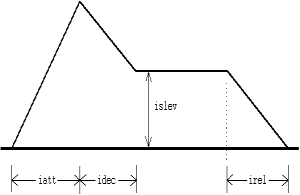
\includegraphics[scale=1]{adsr} 


 Picture of an ADSR envelope.


  The length of the sustain is calculated from the length of the note. This means \emph{adsr}
 is not suitable for use with MIDI events. The opcode \emph{madsr}
 uses the \emph{linsegr}
 mechanism, and so can be used in MIDI applications. 


 \emph{adsr}
 is new in Csound version 3.49. 
\subsection*{Examples}


  Here is an example of the adsr opcode. It uses the files \emph{adsr.orc}
 and \emph{adsr.sco}
. 


 \textbf{Example 1. Example of the adsr opcode.}

\begin{lstlisting}
/* adsr.orc */
; Initialize the global variables.
sr = 44100
kr = 4410
ksmps = 10
nchnls = 1

; Instrument #1 - a simple instrument.
instr 1
  ; Set the amplitude.
  kamp init 20000
  ; Get the frequency from the fourth p-field.
  kcps = cpspch(p4)

  a1 vco kamp, kcps, 1
  out a1
endin

; Instrument #2 - instrument with an ADSR envelope.
instr 2
  iatt = 0.05
  idec =  0.5
  islev = 0.08
  irel = 0.008

  ; Create an amplitude envelope.
  kenv adsr iatt, idec, islev, irel
  kamp = kenv * 20000

  ; Get the frequency from the fourth p-field.
  kcps = cpspch(p4)

  a1 vco kamp, kcps, 1
  out a1
endin
/* adsr.orc */
        
\end{lstlisting}
\begin{lstlisting}
/* adsr.sco */
; Table #1, a sine wave.
f 1 0 16384 10 1

; Set the tempo to 120 beats per minute.
t 0 120

; Play a melody with Instrument #1.
; p4 = frequency in pitch-class notation.
i  1  0   1  8.04
i  1  1   1  8.04
i  1  2   1  8.05
i  1  3   1  8.07
i  1  4   1  8.07
i  1  5   1  8.05
i  1  6   1  8.04
i  1  7   1  8.02
i  1  8   1  8.00
i  1  9   1  8.00
i  1  10  1  8.02
i  1  11  1  8.04
i  1  12  2  8.04
i  1  14  2  8.02

; Repeat the melody with Instrument #2.
; p4 = frequency in pitch-class notation.
i  2  16  1  8.04
i  2  17  1  8.04
i  2  18  1  8.05
i  2  19  1  8.07
i  2  20  1  8.07
i  2  21  1  8.05
i  2  22  1  8.04
i  2  23  1  8.02
i  2  24  1  8.00
i  2  25  1  8.00
i  2  26  1  8.02
i  2  27  1  8.04
i  2  28  2  8.04
i  2  30  2  8.02
e
/* adsr.sco */
        
\end{lstlisting}
\subsection*{See Also}


 \emph{madsr}
, \emph{mxadsr}
, \emph{xadsr}

\subsection*{Credits}


 Example written by Kevin Conder.
%\hline 


\begin{comment}
\begin{tabular}{lcr}
Previous &Home &Next \\
active &Up &adsyn

\end{tabular}


\end{document}
\end{comment}

\newpage
\begin{comment}
\documentclass[10pt]{article}
\usepackage{fullpage, graphicx, url}
\setlength{\parskip}{1ex}
\setlength{\parindent}{0ex}
\title{adsyn}
\begin{document}


\begin{tabular}{ccc}
The Alternative Csound Reference Manual & & \\
Previous & &Next

\end{tabular}

%\hline 
\end{comment}
\section{adsyn}
adsyn�--� Output is an additive set of individually controlled sinusoids, using an oscillator bank. \subsection*{Description}


  Output is an additive set of individually controlled sinusoids, using an oscillator bank. 
\subsection*{Syntax}


 ar \textbf{adsyn}
 kamod, kfmod, ksmod, ifilcod
\subsection*{Initialization}


 \emph{ifilcod}
 -- integer or character-string denoting a control-file derived from analysis of an audio signal. An integer denotes the suffix of a file \emph{adsyn.m}
 or \emph{pvoc.m}
; a character-string (in double quotes) gives a filename, optionally a full pathname. If not fullpath, the file is sought first in the current directory, then in the one given by the environment variable \emph{SADIR}
 (if defined). \emph{adsyn}
 control contains breakpoint amplitude- and frequency-envelope values organized for oscillator resynthesis, while \emph{pvoc}
 control contains similar data organized for fft resynthesis. Memory usage depends on the size of the files involved, which are read and held entirely in memory during computation but are shared by multiple calls (see also \emph{lpread}
). 
\subsection*{Performance}


 \emph{kamod}
 -- amplitude factor of the contributing partials. 


 \emph{kfmod}
 -- frequency factor of the contributing partials. It is a control-rate transposition factor: a value of 1 incurs no transposition, 1.5 transposes up a perfect fifth, and .5 down an octave. 


 \emph{ksmod}
 -- speed factor of the contributing partials. 


 \emph{adsyn}
 synthesizes complex time-varying timbres through the method of additive synthesis. Any number of sinusoids, each individually controlled in frequency and amplitude, can be summed by high-speed arithmetic to produce a high-fidelity result. 


  Component sinusoids are described by a control file describing amplitude and frequency tracks in millisecond breakpoint fashion. Tracks are defined by sequences of 16-bit binary integers: 


 -1,�time,�amp,�time,�amp,...�\\ 
 -2,�time,�freq,�time,�freq,...\\ 
 ������
 such as from hetrodyne filter analysis of an audio file. (For details see \emph{hetro}
.) The instantaneous amplitude and frequency values are used by an internal fixed-point oscillator that adds each active partial into an accumulated output signal. While there is a practical limit (limit removed in version 3.47) on the number of contributing partials, there is no restriction on their behavior over time. Any sound that can be described in terms of the behavior of sinusoids can be synthesized by \emph{adsyn}
 alone. 

  Sound described by an \emph{adsyn}
 control file can also be modified during re-synthesis. The signals \emph{kamod,}
 \emph{kfmod}
, \emph{ksmod}
 will modify the amplitude, frequency, and speed of contributing partials. These are multiplying factors, with \emph{kfmod}
 modifying the frequency and \emph{ksmod}
 modifying the \emph{speed}
 with which the millisecond breakpoint line-segments are traversed. Thus .7, 1.5, and 2 will give rise to a softer sound, a perfect fifth higher, but only half as long. The values 1,1,1 will leave the sound unmodified. Each of these inputs can be a control signal. 
\subsection*{Examples}


  Here is an example of the adsyn opcode. It uses the files \emph{adsyn.orc}
, \emph{adsyn.sco}
, and \emph{kickroll.het}
. The file ``kickroll.het'' was created by using the \emph{hetro}
 utility with the audio file \emph{kickroll.wav}
. 


 \textbf{Example 1. Example of the adsyn opcode.}

\begin{lstlisting}
/* adsyn.orc */
; Initialize the global variables.
sr = 44100
kr = 4410
ksmps = 10
nchnls = 1

; Instrument #1.
instr 1
  ; If the modulation amounts are set to 1, adsyn
  ; will not perform any special modulation.
  kamod init 1
  kfmod init 1
  ksmod init 1

  ; Re-synthesizes the file "kickroll.het".
  a1 adsyn kamod, kfmod, ksmod, "kickroll.het"

  out a1 * 32768
endin
/* adsyn.orc */
        
\end{lstlisting}
\begin{lstlisting}
/* adsyn.sco */
; Play Instrument #1 for one second.
i 1 0 1
e
/* adsyn.sco */
        
\end{lstlisting}
\subsection*{Credits}


 Example written by Kevin Conder.
%\hline 


\begin{comment}
\begin{tabular}{lcr}
Previous &Home &Next \\
adsr &Up &adsynt

\end{tabular}


\end{document}
\end{comment}

\newpage
\begin{comment}
\documentclass[10pt]{article}
\usepackage{fullpage, graphicx, url}
\setlength{\parskip}{1ex}
\setlength{\parindent}{0ex}
\title{adsynt}
\begin{document}


\begin{tabular}{ccc}
The Alternative Csound Reference Manual & & \\
Previous & &Next

\end{tabular}

%\hline 
\end{comment}
\section{adsynt}
adsynt�--� Performs additive synthesis with an arbitrary number of partials, not necessarily harmonic. \subsection*{Description}


  Performs additive synthesis with an arbitrary number of partials, not necessarily harmonic. 
\subsection*{Syntax}


 ar \textbf{adsynt}
 kamp, kcps, iwfn, ifreqfn, iampfn, icnt [, iphs]
\subsection*{Initialization}


 \emph{iwfn}
 -- table containing a waveform, usually a sine. Table values are not interpolated for performance reasons, so larger tables provide better quality. 


 \emph{ifreqfn}
 -- table containing frequency values for each partial. \emph{ifreqfn}
 may contain beginning frequency values for each partial, but is usually used for generating parameters at runtime with \emph{tablew}
. Frequencies must be relative to \emph{kcps}
. Size must be at least \emph{icnt}
. 


 \emph{iampfn}
 -- table containing amplitude values for each partial. \emph{iampfn}
 may contain beginning amplitude values for each partial, but is usually used for generating parameters at runtime with \emph{tablew}
. Amplitudes must be relative to \emph{kamp}
. Size must be at least \emph{icnt}
. 


 \emph{icnt}
 -- number of partials to be generated 


 \emph{iphs}
 -- initial phase of each oscillator, if \emph{iphs}
 = -1, initialization is skipped. If \emph{iphs}
 $>$ 1, all phases will be initialized with a random value. 
\subsection*{Performance}


 \emph{kamp}
 -- amplitude of note 


 \emph{kcps}
 -- base frequency of note. Partial frequencies will be relative to \emph{kcps}
. 


  Frequency and amplitude of each partial is given in the two tables provided. The purpose of this opcode is to have an instrument generate synthesis parameters at k-rate and write them to global parameter tables with the \emph{tablew}
 opcode. 
\subsection*{Examples}


  Here is an example of the adsynt opcode. It uses the files \emph{adsynt.orc}
 and \emph{adsynt.sco}
. These two instruments perform additive synthesis. The output of each sounds like a Tibetan bowl. The first one is static, as parameters are only generated at init-time. In the second one, parameters are continuously changed. 


 \textbf{Example 1. Example of the adsynt opcode.}

\begin{lstlisting}
/* adsynt.orc */
; Initialize the global variables.
sr = 44100
kr = 4410
ksmps = 10
nchnls = 1

; Generate a sinewave table.
giwave ftgen 1, 0, 1024, 10, 1
; Generate two empty tables for adsynt.
gifrqs ftgen 2, 0, 32, 7, 0, 32, 0
; A table for freqency and amp parameters.
giamps ftgen 3, 0, 32, 7, 0, 32, 0
  
; Generates parameters at init time
instr 1
  ; Generate 10 voices.
  icnt = 10 
  ; Init loop index.
  index = 0 

; Loop only executed at init time.
loop: 
  ; Define non-harmonic partials.
  ifreq pow index + 1, 1.5 
  ; Define amplitudes.
  iamp = 1 / (index+1) 
  ; Write to tables.
  tableiw ifreq, index, gifrqs 
  ; Used by adsynt.
  tableiw iamp, index, giamps 
  
  index = index + 1
  ; Do loop/
  if (index < icnt) igoto loop 
  
  asig adsynt 5000, 150, giwave, gifrqs, giamps, icnt
  out asig
endin

; Generates parameters every k-cycle.
instr 2 
  ; Generate 10 voices.
  icnt = 10 
  ; Reset loop index.
  kindex = 0

; Loop executed every k-cycle.
loop:
  ; Generate lfo for frequencies.
  kspeed  pow kindex + 1, 1.6
  ; Individual phase for each voice.
  kphas phasorbnk kspeed * 0.7, kindex, icnt
  klfo table kphas, giwave, 1
  ; Arbitrary parameter twiddling...
  kdepth pow 1.4, kindex
  kfreq pow kindex + 1, 1.5
  kfreq = kfreq + klfo*0.006*kdepth

  ; Write freqs to table for adsynt.
  tablew kfreq, kindex, gifrqs 
  
  ; Generate lfo for amplitudes.
  kspeed  pow kindex + 1, 0.8
  ; Individual phase for each voice.
  kphas phasorbnk kspeed*0.13, kindex, icnt, 2
  klfo table kphas, giwave, 1
  ; Arbitrary parameter twiddling...
  kamp pow 1 / (kindex + 1), 0.4
  kamp = kamp * (0.3+0.35*(klfo+1))

  ; Write amps to table for adsynt.
  tablew kamp, kindex, giamps
  
  kindex = kindex + 1
  ; Do loop.
  if (kindex < icnt) kgoto loop

  asig adsynt 5000, 150, giwave, gifrqs, giamps, icnt
  out asig
endin
/* adsynt.orc */
        
\end{lstlisting}
\begin{lstlisting}
/* adsynt.sco */
; Play Instrument #1 for 2.5 seconds.
i 1 0 2.5
; Play Instrument #2 for 2.5 seconds.
i 2 3 2.5
e
/* adsynt.sco */
        
\end{lstlisting}
\subsection*{Credits}


 


 


\begin{tabular}{ccc}
Author: Peter Neub\"acker &Munich, Germany &August, 1999

\end{tabular}



 


 New in Csound version 3.58
%\hline 


\begin{comment}
\begin{tabular}{lcr}
Previous &Home &Next \\
adsyn &Up &aexprand

\end{tabular}


\end{document}
\end{comment}

\newpage
\begin{comment}
\documentclass[10pt]{article}
\usepackage{fullpage, graphicx, url}
\setlength{\parskip}{1ex}
\setlength{\parindent}{0ex}
\title{aexprand}
\begin{document}


\begin{tabular}{ccc}
The Alternative Csound Reference Manual & & \\
Previous & &Next

\end{tabular}

%\hline 
\end{comment}
\section{aexprand}
aexprand�--� Deprecated. \subsection*{Description}


  Deprecated as of version 3.49. Use the \emph{exprand}
 opcode instead. 
%\hline 


\begin{comment}
\begin{tabular}{lcr}
Previous &Home &Next \\
adsynt &Up &aftouch

\end{tabular}


\end{document}
\end{comment}

\newpage
\begin{comment}
\documentclass[10pt]{article}
\usepackage{fullpage, graphicx, url}
\setlength{\parskip}{1ex}
\setlength{\parindent}{0ex}
\title{aftouch}
\begin{document}


\begin{tabular}{ccc}
The Alternative Csound Reference Manual & & \\
Previous & &Next

\end{tabular}

%\hline 
\end{comment}
\section{aftouch}
aftouch�--� Get the current after-touch value for this channel. \subsection*{Description}


  Get the current after-touch value for this channel. 
\subsection*{Syntax}


 kaft \textbf{aftouch}
 [imin] [, imax]
\subsection*{Initialization}


 \emph{imin}
 (optional, default=0) -- minimum limit on values obtained. 


 \emph{imax}
 (optional, default=127) -- maximum limit on values obtained. 
\subsection*{Performance}


  Get the current after-touch value for this channel. Note that this access to pitch-bend data is independent of the MIDI pitch, enabling the value here to be used for any arbitrary purpose. 
\subsection*{Examples}


  Here is an example of the aftouch opcode. It uses the files \emph{aftouch.orc}
 and \emph{aftouch.sco}
. 


 \textbf{Example 1. Example of the aftouch opcode.}

\begin{lstlisting}
/* aftouch.orc */
; Initialize the global variables.
sr = 44100
kr = 4410
ksmps = 10
nchnls = 1

; Instrument #1.
instr 1
  k1 aftouch

  printk2 k1
endin
/* aftouch.orc */
        
\end{lstlisting}
\begin{lstlisting}
/* aftouch.sco */
; Play Instrument #1 for 12 seconds.
i 1 0 12
e
/* aftouch.sco */
        
\end{lstlisting}
\subsection*{See Also}


 \emph{ampmidi}
, \emph{cpsmidi}
, \emph{cpsmidib}
, \emph{midictrl}
, \emph{notnum}
, \emph{octmidi}
, \emph{octmidib}
, \emph{pchbend}
, \emph{pchmidi}
, \emph{pchmidib}
, \emph{veloc}

\subsection*{Credits}


 


 


\begin{tabular}{ccc}
Author: Barry L. Vercoe - Mike Berry &MIT - Mills &May 1997

\end{tabular}



 


 Example written by Kevin Conder.
%\hline 


\begin{comment}
\begin{tabular}{lcr}
Previous &Home &Next \\
aexprand &Up &agauss

\end{tabular}


\end{document}
\end{comment}

\newpage
\begin{comment}
\documentclass[10pt]{article}
\usepackage{fullpage, graphicx, url}
\setlength{\parskip}{1ex}
\setlength{\parindent}{0ex}
\title{agauss}
\begin{document}


\begin{tabular}{ccc}
The Alternative Csound Reference Manual & & \\
Previous & &Next

\end{tabular}

%\hline 
\end{comment}
\section{agauss}
agauss�--� Deprecated. \subsection*{Description}


  Deprecated as of version 3.49. Use the \emph{gauss}
 opcode instead. 
%\hline 


\begin{comment}
\begin{tabular}{lcr}
Previous &Home &Next \\
aftouch &Up &agogobel

\end{tabular}


\end{document}
\end{comment}

\newpage
\begin{comment}
\documentclass[10pt]{article}
\usepackage{fullpage, graphicx, url}
\setlength{\parskip}{1ex}
\setlength{\parindent}{0ex}
\title{agogobel}
\begin{document}


\begin{tabular}{ccc}
The Alternative Csound Reference Manual & & \\
Previous & &Next

\end{tabular}

%\hline 
\end{comment}
\section{agogobel}
agogobel�--� Deprecated. \subsection*{Description}


  Deprecated as of version 3.52. Use the \emph{gogobel}
 opcode instead. 
%\hline 


\begin{comment}
\begin{tabular}{lcr}
Previous &Home &Next \\
agauss &Up &alinrand

\end{tabular}


\end{document}
\end{comment}

\newpage
\begin{comment}
\documentclass[10pt]{article}
\usepackage{fullpage, graphicx, url}
\setlength{\parskip}{1ex}
\setlength{\parindent}{0ex}
\title{alinrand}
\begin{document}


\begin{tabular}{ccc}
The Alternative Csound Reference Manual & & \\
Previous & &Next

\end{tabular}

%\hline 
\end{comment}
\section{alinrand}
alinrand�--� Deprecated. \subsection*{Description}


  Deprecated as of version 3.49. Use the \emph{linrand}
 opcode instead. 
%\hline 


\begin{comment}
\begin{tabular}{lcr}
Previous &Home &Next \\
agogobel &Up &alpass

\end{tabular}


\end{document}
\end{comment}

\newpage
\begin{comment}
\documentclass[10pt]{article}
\usepackage{fullpage, graphicx, url}
\setlength{\parskip}{1ex}
\setlength{\parindent}{0ex}
\title{alpass}
\begin{document}


\begin{tabular}{ccc}
The Alternative Csound Reference Manual & & \\
Previous & &Next

\end{tabular}

%\hline 
\end{comment}
\section{alpass}
alpass�--� Reverberates an input signal with a flat frequency response. \subsection*{Description}


  Reverberates an input signal with a flat frequency response. 
\subsection*{Syntax}


 ar \textbf{alpass}
 asig, krvt, ilpt [, iskip] [, insmps]
\subsection*{Initialization}


 \emph{ilpt}
 -- loop time in seconds, which determines the ``echo density'' of the reverberation. This in turn characterizes the ``color'' of the filter whose frequency response curve will contain \emph{ilpt}
 * \emph{sr}
/2 peaks spaced evenly between 0 and \emph{sr}
/2 (the Nyquist frequency). Loop time can be as large as available memory will permit. The space required for an \emph{n}
 second loop is 4\emph{n}
*\emph{sr}
 bytes. The delay space is allocated and returned as in \emph{delay}
. 


 \emph{iskip}
 (optional, default=0) -- initial disposition of delay-loop data space (cf. \emph{reson}
). The default value is 0. 


 \emph{insmps}
 (optional, default=0) -- delay amount, as a number of samples. 
\subsection*{Performance}


 \emph{krvt}
 -- the reverberation time (defined as the time in seconds for a signal to decay to 1/1000, or 60dB down from its original amplitude). 


  This filter reiterates the input with an echo density determined by loop time \emph{ilpt}
. The attenuation rate is independent and is determined by \emph{krvt}
, the reverberation time (defined as the time in seconds for a signal to decay to 1/1000, or 60dB down from its original amplitude). Output will begin to appear immediately. 
\subsection*{Examples}


  Here is an example of the alpass opcode. It uses the files \emph{alpass.orc}
 and \emph{alpass.sco}
. 


 \textbf{Example 1. Example of the alpass opcode.}

\begin{lstlisting}
/* alpass.orc */
; Initialize the global variables.
sr = 44100
kr = 4410
ksmps = 10
nchnls = 1

; Initialize the audio mixer.
gamix init 0 

; Instrument #1.
instr 1 
  ; Generate a source signal.
  a1 oscili 30000, cpspch(p4), 1
  ; Output the direct sound.
  out a1  

  ; Add the source signal to the audio mixer.
  gamix = gamix + a1 
endin

; Instrument #99 (highest instr number executed last)
instr 99 
  krvt = 1.5
  ilpt = 0.1

  ; Filter the mixed signal.
  a99 alpass gamix, krvt, ilpt
  ; Output the result.
  out a99 

  ; Empty the mixer for the next pass.
  gamix = 0 
endin
/* alpass.orc */
        
\end{lstlisting}
\begin{lstlisting}
/* alpass.sco */
; Table #1, a sine wave.
f 1 0 128 10 1

; p4 = frequency (in a pitch-class)
; Play Instrument #1 for a tenth of a second, p4=7.00
i 1 0 0.1 7.00
; Play Instrument #1 for a tenth of a second, p4=7.02
i 1 1 0.1 7.02
; Play Instrument #1 for a tenth of a second, p4=7.04
i 1 2 0.1 7.04
; Play Instrument #1 for a tenth of a second, p4=7.06
i 1 3 0.1 7.06

; Make sure the filter remains active.
i 99 0 5
e
/* alpass.sco */
        
\end{lstlisting}
\subsection*{See Also}


 \emph{comb}
, \emph{reverb}
, \emph{valpass}
, \emph{vcomb}

\subsection*{Credits}


 


 


\begin{tabular}{cccc}
Author: William ``Pete'' Moss (\emph{vcomb}
 and \emph{valpass}
) &University of Texas at Austin &Austin, Texas USA &January 2002

\end{tabular}



 


 Example written by Kevin Conder.
%\hline 


\begin{comment}
\begin{tabular}{lcr}
Previous &Home &Next \\
alinrand &Up &ampdb

\end{tabular}


\end{document}
\end{comment}

\newpage
\begin{comment}
\documentclass[10pt]{article}
\usepackage{fullpage, graphicx, url}
\setlength{\parskip}{1ex}
\setlength{\parindent}{0ex}
\title{ampdb}
\begin{document}


\begin{tabular}{ccc}
The Alternative Csound Reference Manual & & \\
Previous & &Next

\end{tabular}

%\hline 
\end{comment}
\section{ampdb}
ampdb�--� Returns the amplitude equivalent of the decibel value x. \subsection*{Description}


  Returns the amplitude equivalent of the decibel value x. Thus: 


 
\begin{itemize}
\item 

 60 dB = 1000

\item 

 66 dB = 1995.262

\item 

 72 dB = 3891.07

\item 

 78 dB = 7943.279

\item 

 84 dB = 15848.926

\item 

 90 dB = 31622.764


\end{itemize}
\subsection*{Syntax}


 \textbf{ampdb}
(x) (no rate restriction)
\subsection*{Examples}


  Here is an example of the ampdb opcode. It uses the files \emph{ampdb.orc}
 and \emph{ampdb.sco}
. 


 \textbf{Example 1. Example of the ampdb opcode.}

\begin{lstlisting}
/* ampdb.orc */
; Initialize the global variables.
sr = 44100
kr = 4410
ksmps = 10
nchnls = 1

; Instrument #1.
instr 1
  idb = 90
  iamp = ampdb(idb)

  print iamp
endin
/* ampdb.orc */
        
\end{lstlisting}
\begin{lstlisting}
/* ampdb.sco */
; Play Instrument #1 for one second.
i 1 0 1
e
/* ampdb.sco */
        
\end{lstlisting}
 Its output should include lines like: \begin{lstlisting}
instr 1:  iamp = 31622.764
      
\end{lstlisting}
\subsection*{See Also}


 \emph{ampdbfs}
, \emph{db}
, \emph{dbamp}
, \emph{dbfsamp}

\subsection*{Credits}


 Example written by Kevin Conder.
%\hline 


\begin{comment}
\begin{tabular}{lcr}
Previous &Home &Next \\
alpass &Up &ampdbfs

\end{tabular}


\end{document}
\end{comment}

\newpage
\begin{comment}
\documentclass[10pt]{article}
\usepackage{fullpage, graphicx, url}
\setlength{\parskip}{1ex}
\setlength{\parindent}{0ex}
\title{ampdbfs}
\begin{document}


\begin{tabular}{ccc}
The Alternative Csound Reference Manual & & \\
Previous & &Next

\end{tabular}

%\hline 
\end{comment}
\section{ampdbfs}
ampdbfs�--� Returns the amplitude equivalent of the decibel value x, which is relative to full scale amplitude. \subsection*{Description}


  Returns the amplitude equivalent of the decibel value x, which is relative to full scale amplitude. Full scale is assumed to be 16 bit. New is Csound version 4.10. 
\subsection*{Syntax}


 \textbf{ampdbfs}
(x) (no rate restriction)
\subsection*{Examples}


  Here is an example of the ampdbfs opcode. It uses the files \emph{ampdbfs.orc}
 and \emph{ampdbfs.sco}
. 


 \textbf{Example 1. Example of the ampdbfs opcode.}

\begin{lstlisting}
/* ampdbfs.orc */
; Initialize the global variables.
sr = 44100
kr = 4410
ksmps = 10
nchnls = 1

; Instrument #1.
instr 1
  idb = -1
  iamp = ampdbfs(idb)

  print iamp
endin
/* ampdbfs.orc */
        
\end{lstlisting}
\begin{lstlisting}
/* ampdbfs.sco */
; Play Instrument #1 for one second.
i 1 0 1
e
/* ampdbfs.sco */
        
\end{lstlisting}
 Its output should include lines like: \begin{lstlisting}
instr 1:  iamp = 29203.621
      
\end{lstlisting}
\subsection*{See Also}


 \emph{ampdb}
, \emph{dbamp}
, \emph{dbfsamp}

\subsection*{Credits}


 Example written by Kevin Conder.
%\hline 


\begin{comment}
\begin{tabular}{lcr}
Previous &Home &Next \\
ampdb &Up &ampmidi

\end{tabular}


\end{document}
\end{comment}

\newpage
\begin{comment}
\documentclass[10pt]{article}
\usepackage{fullpage, graphicx, url}
\setlength{\parskip}{1ex}
\setlength{\parindent}{0ex}
\title{ampmidi}
\begin{document}


\begin{tabular}{ccc}
The Alternative Csound Reference Manual & & \\
Previous & &Next

\end{tabular}

%\hline 
\end{comment}
\section{ampmidi}
ampmidi�--� Get the velocity of the current MIDI event. \subsection*{Description}


  Get the velocity of the current MIDI event. 
\subsection*{Syntax}


 iamp \textbf{ampmidi}
 iscal [, ifn]
\subsection*{Initialization}


 \emph{iscal}
 -- i-time scaling factor 


 \emph{ifn}
 (optional, default=0) -- function table number of a normalized translation table, by which the incoming value is first interpreted. The default value is 0, denoting no translation. 
\subsection*{Performance}


  Get the velocity of the current MIDI event, optionally pass it through a normalized translation table, and return an amplitude value in the range 0 - \emph{iscal}
. 
\subsection*{Examples}


  Here is an example of the ampmidi opcode. It uses the files \emph{ampmidi.orc}
 and \emph{ampmidi.sco}
. 


 \textbf{Example 1. Example of the ampmidi opcode.}

\begin{lstlisting}
/* ampmidi.orc */
; Initialize the global variables.
sr = 44100
kr = 4410
ksmps = 10
nchnls = 1

; Instrument #1.
instr 1
  ; Scale the amplitude between 0 and 1.
  i1 ampmidi 1

  print i1
endin
/* ampmidi.orc */
        
\end{lstlisting}
\begin{lstlisting}
/* ampmidi.sco */
; Play Instrument #1 for 12 seconds.
i 1 0 12
e
/* ampmidi.sco */
        
\end{lstlisting}
\subsection*{See Also}


 \emph{aftouch}
, \emph{cpsmidi}
, \emph{cpsmidib}
, \emph{midictrl}
, \emph{notnum}
, \emph{octmidi}
, \emph{octmidib}
, \emph{pchbend}
, \emph{pchmidi}
, \emph{pchmidib}
, \emph{veloc}

\subsection*{Credits}


 


 


\begin{tabular}{ccc}
Author: Barry L. Vercoe - Mike Berry &MIT - Mills &May 1997

\end{tabular}



 


 Example written by Kevin Conder.
%\hline 


\begin{comment}
\begin{tabular}{lcr}
Previous &Home &Next \\
ampdbfs &Up &apcauchy

\end{tabular}


\end{document}
\end{comment}

\newpage
\begin{comment}
\documentclass[10pt]{article}
\usepackage{fullpage, graphicx, url}
\setlength{\parskip}{1ex}
\setlength{\parindent}{0ex}
\title{apcauchy}
\begin{document}


\begin{tabular}{ccc}
The Alternative Csound Reference Manual & & \\
Previous & &Next

\end{tabular}

%\hline 
\end{comment}
\section{apcauchy}
apcauchy�--� Deprecated. \subsection*{Description}


  Deprecated as of version 3.49. Use the \emph{pcauchy}
 opcode instead. 
%\hline 


\begin{comment}
\begin{tabular}{lcr}
Previous &Home &Next \\
ampmidi &Up &apoisson

\end{tabular}


\end{document}
\end{comment}

\newpage
\begin{comment}
\documentclass[10pt]{article}
\usepackage{fullpage, graphicx, url}
\setlength{\parskip}{1ex}
\setlength{\parindent}{0ex}
\title{apoisson}
\begin{document}


\begin{tabular}{ccc}
The Alternative Csound Reference Manual & & \\
Previous & &Next

\end{tabular}

%\hline 
\end{comment}
\section{apoisson}
apoisson�--� Deprecated. \subsection*{Description}


  Deprecated as of version 3.49. Use the \emph{poisson}
 opcode instead. 
%\hline 


\begin{comment}
\begin{tabular}{lcr}
Previous &Home &Next \\
apcauchy &Up &apow

\end{tabular}


\end{document}
\end{comment}

\newpage
\begin{comment}
\documentclass[10pt]{article}
\usepackage{fullpage, graphicx, url}
\setlength{\parskip}{1ex}
\setlength{\parindent}{0ex}
\title{apow}
\begin{document}


\begin{tabular}{ccc}
The Alternative Csound Reference Manual & & \\
Previous & &Next

\end{tabular}

%\hline 
\end{comment}
\section{apow}
apow�--� Deprecated. \subsection*{Description}


  Deprecated as of version 3.48. Use the \emph{pow}
 opcode instead. 
%\hline 


\begin{comment}
\begin{tabular}{lcr}
Previous &Home &Next \\
apoisson &Up &areson

\end{tabular}


\end{document}
\end{comment}

\newpage
\begin{comment}
\documentclass[10pt]{article}
\usepackage{fullpage, graphicx, url}
\setlength{\parskip}{1ex}
\setlength{\parindent}{0ex}
\title{areson}
\begin{document}


\begin{tabular}{ccc}
The Alternative Csound Reference Manual & & \\
Previous & &Next

\end{tabular}

%\hline 
\end{comment}
\section{areson}
areson�--� A notch filter whose transfer functions are the complements of the reson opcode. \subsection*{Description}


  A notch filter whose transfer functions are the complements of the reson opcode. 
\subsection*{Syntax}


 ar \textbf{areson}
 asig, kcf, kbw [, iscl] [, iskip]
\subsection*{Initialization}


 \emph{iscl}
 (optional, default=0) -- coded scaling factor for resonators. A value of 1 signifies a peak response factor of 1, i.e. all frequencies other than kcf are attenuated in accordance with the (normalized) response curve. A value of 2 raises the response factor so that its overall RMS value equals 1. (This intended equalization of input and output power assumes all frequencies are physically present; hence it is most applicable to white noise.) A zero value signifies no scaling of the signal, leaving that to some later adjustment (see \emph{balance}
). The default value is 0. 


 \emph{iskip}
 (optional, default=0) -- initial disposition of internal data space. Since filtering incorporates a feedback loop of previous output, the initial status of the storage space used is significant. A zero value will clear the space; a non-zero value will allow previous information to remain. The default value is 0. 
\subsection*{Performance}


 \emph{ar}
 -- the output signal at audio rate. 


 \emph{asig}
 -- the input signal at audio rate. 


 \emph{kcf}
 -- the center frequency of the filter, or frequency position of the peak response. 


 \emph{kbw}
 -- bandwidth of the filter (the Hz difference between the upper and lower half-power points). 


 \emph{areson}
 is a filter whose transfer functions is the complement of \emph{reson}
. Thus \emph{areson}
 is a notch filter whose transfer functions represents the ``filtered out'' aspects of their complements. However, power scaling is not normalized in \emph{areson}
 but remains the true complement of the corresponding unit. Thus an audio signal, filtered by parallel matching \emph{reson}
 and \emph{areson}
 units, would under addition simply reconstruct the original spectrum. 


  This property is particularly useful for controlled mixing of different sources (see \emph{lpreson}
). Complex response curves such as those with multiple peaks can be obtained by using a bank of suitable filters in series. (The resultant response is the product of the component responses.) In such cases, the combined attenuation may result in a serious loss of signal power, but this can be regained by the use of \emph{balance}
. 
\subsection*{Examples}


  Here is an example of the areson opcode. It uses the files \emph{areson.orc}
 and \emph{areson.sco}
. 


 \textbf{Example 1. Example of the areson opcode.}

\begin{lstlisting}
/* areson.orc */
; Initialize the global variables.
sr = 22050
kr = 2205
ksmps = 10
nchnls = 1

; Instrument #1 - an unfiltered noise waveform.
instr 1
  ; Generate a white noise signal.
  asig rand 20000

  out asig
endin


; Instrument #2 - a filtered noise waveform.
instr 2
  ; Generate a white noise signal.
  asig rand 20000

  ; Filter it using the areson opcode.
  kcf init 1000
  kbw init 100
  afilt areson asig, kcf, kbw

  ; Clip the filtered signal's amplitude to 85 dB.
  a1 clip afilt, 2, ampdb(85)
  out a1
endin
/* areson.orc */
        
\end{lstlisting}
\begin{lstlisting}
/* areson.sco */
; Play Instrument #1 for two seconds.
i 1 0 2
; Play Instrument #2 for two seconds.
i 2 2 2
e
/* areson.sco */
        
\end{lstlisting}
\subsection*{See Also}


 \emph{aresonk}
, \emph{atone}
, \emph{atonek}
, \emph{port}
, \emph{portk}
, \emph{reson}
, \emph{resonk}
, \emph{tone}
, \emph{tonek}

%\hline 


\begin{comment}
\begin{tabular}{lcr}
Previous &Home &Next \\
apow &Up &aresonk

\end{tabular}


\end{document}
\end{comment}

\newpage
\begin{comment}
\documentclass[10pt]{article}
\usepackage{fullpage, graphicx, url}
\setlength{\parskip}{1ex}
\setlength{\parindent}{0ex}
\title{aresonk}
\begin{document}


\begin{tabular}{ccc}
The Alternative Csound Reference Manual & & \\
Previous & &Next

\end{tabular}

%\hline 
\end{comment}
\section{aresonk}
aresonk�--� A notch filter whose transfer functions are the complements of the reson opcode. \subsection*{Description}


  A notch filter whose transfer functions are the complements of the reson opcode. 
\subsection*{Syntax}


 kr \textbf{aresonk}
 ksig, kcf, kbw [, iscl] [, iskip]
\subsection*{Initialization}


 \emph{iscl}
 (optional, default=0) -- coded scaling factor for resonators. A value of 1 signifies a peak response factor of 1, i.e. all frequencies other than kcf are attenuated in accordance with the (normalized) response curve. A value of 2 raises the response factor so that its overall RMS value equals 1. (This intended equalization of input and output power assumes all frequencies are physically present; hence it is most applicable to white noise.) A zero value signifies no scaling of the signal, leaving that to some later adjustment (see \emph{balance}
). The default value is 0. 


 \emph{iskip}
 (optional, default=0) -- initial disposition of internal data space. Since filtering incorporates a feedback loop of previous output, the initial status of the storage space used is significant. A zero value will clear the space; a non-zero value will allow previous information to remain. The default value is 0. 
\subsection*{Performance}


 \emph{kr}
 -- the output signal at control-rate. 


 \emph{ksig}
 -- the input signal at control-rate. 


 \emph{kcf}
 -- the center frequency of the filter, or frequency position of the peak response. 


 \emph{kbw}
 -- bandwidth of the filter (the Hz difference between the upper and lower half-power points). 


 \emph{aresonk}
 is a filter whose transfer functions is the complement of \emph{reson}
. Thus \emph{aresonk}
 is a notch filter whose transfer functions represents the ``filtered out'' aspects of their complements. However, power scaling is not normalized in \emph{aresonk}
 but remains the true complement of the corresponding unit. 
\subsection*{See Also}


 \emph{areson}
, \emph{atone}
, \emph{atonek}
, \emph{port}
, \emph{portk}
, \emph{reson}
, \emph{resonk}
, \emph{tone}
, \emph{tonek}

%\hline 


\begin{comment}
\begin{tabular}{lcr}
Previous &Home &Next \\
areson &Up &atone

\end{tabular}


\end{document}
\end{comment}

\newpage
\begin{comment}
\documentclass[10pt]{article}
\usepackage{fullpage, graphicx, url}
\setlength{\parskip}{1ex}
\setlength{\parindent}{0ex}
\title{=}
\begin{document}


\begin{tabular}{ccc}
The Alternative Csound Reference Manual & & \\
Previous & &Next

\end{tabular}

%\hline 
\end{comment}
\section{=}
=�--� Performs a simple assignment. \subsection*{Syntax}


 ar \textbf{=}
 xarg


 ir \textbf{=}
 iarg


 kr \textbf{=}
 karg
\subsection*{Description}


  Performs a simple assignment. 
\subsection*{Initialization}


 \emph{=}
 (simple assignment) - Put the value of the expression \emph{iarg}
 (\emph{karg, xarg}
) into the named result. This provides a means of saving an evaluated result for later use. 
\subsection*{Examples}


  Here is an example of the assign opcode. It uses the files \emph{assign.orc}
 and \emph{assign.sco}
. 


 \textbf{Example 1. Example of the assign opcode.}

\begin{lstlisting}
/* assign.orc */
; Initialize the global variables.
sr = 44100
kr = 4410
ksmps = 10
nchnls = 1

; Instrument #1.
instr 1
  ; Assign a value to the variable i1.
  i1 = 1234

  ; Print the value of the i1 variable.
  print i1
endin
/* assign.orc */
        
\end{lstlisting}
\begin{lstlisting}
/* assign.sco */
; Play Instrument #1 for one second.
i 1 0 1
e
/* assign.sco */
        
\end{lstlisting}
 Its output should include a line like this: \begin{lstlisting}
instr 1:  i1 = 1234.000
      
\end{lstlisting}
\subsection*{See Also}


 \emph{divz}
, \emph{init}
, \emph{tival}

\subsection*{Credits}


 Example written by Kevin Conder.
%\hline 


\begin{comment}
\begin{tabular}{lcr}
Previous &Home &Next \\
/ &Up &==

\end{tabular}


\end{document}
\end{comment}

\newpage
\begin{comment}
\documentclass[10pt]{article}
\usepackage{fullpage, graphicx, url}
\setlength{\parskip}{1ex}
\setlength{\parindent}{0ex}
\title{atone}
\begin{document}


\begin{tabular}{ccc}
The Alternative Csound Reference Manual & & \\
Previous & &Next

\end{tabular}

%\hline 
\end{comment}
\section{atone}
atone�--� A notch filter whose transfer functions are the complements of the tone opcode. \subsection*{Description}


  A notch filter whose transfer functions are the complements of the tone opcode. 
\subsection*{Syntax}


 ar \textbf{atone}
 asig, khp [, iskip]
\subsection*{Initialization}


 \emph{iskip}
 (optional, default=0) -- initial disposition of internal data space. Since filtering incorporates a feedback loop of previous output, the initial status of the storage space used is significant. A zero value will clear the space; a non-zero value will allow previous information to remain. The default value is 0. 
\subsection*{Performance}


 \emph{ar}
 -- the output signal at audio rate. 


 \emph{asig}
 -- the input signal at audio rate. 


 \emph{khp}
 -- the response curve's half-power point, in Hertz. Half power is defined as peak power / root 2. 


 \emph{atone}
 is a filter whose transfer functions is the complement of \emph{tone}
. \emph{atone}
 is thus a form of high-pass filter whose transfer functions represent the ``filtered out'' aspects of their complements. However, power scaling is not normalized in \emph{atone}
 but remains the true complement of the corresponding unit. Thus an audio signal, filtered by parallel matching \emph{tone}
 and \emph{atone}
 units, would under addition simply reconstruct the original spectrum. 


  This property is particularly useful for controlled mixing of different sources (see \emph{lpreson}
). Complex response curves such as those with multiple peaks can be obtained by using a bank of suitable filters in series. (The resultant response is the product of the component responses.) In such cases, the combined attenuation may result in a serious loss of signal power, but this can be regained by the use of \emph{balance}
. 
\subsection*{Examples}


  Here is an example of the atone opcode. It uses the files \emph{atone.orc}
 and \emph{atone.sco}
. 


 \textbf{Example 1. Example of the atone opcode.}

\begin{lstlisting}
/* atone.orc */
; Initialize the global variables.
sr = 22050
kr = 2205
ksmps = 10
nchnls = 1

; Instrument #1 - an unfiltered noise waveform.
instr 1
  ; Generate a white noise signal.
  asig rand 20000

  out asig
endin


; Instrument #2 - a filtered noise waveform.
instr 2
  ; Generate a white noise signal.
  asig rand 20000

  ; Filter it using the atone opcode.
  khp init 2000
  afilt atone asig, khp

  ; Clip the filtered signal's amplitude to 85 dB.
  a1 clip afilt, 2, ampdb(85)
  out a1
endin
/* atone.orc */
        
\end{lstlisting}
\begin{lstlisting}
/* atone.sco */
; Play Instrument #1 for two seconds.
i 1 0 2
; Play Instrument #2 for two seconds.
i 2 2 2
e
/* atone.sco */
        
\end{lstlisting}
\subsection*{See Also}


 \emph{areson}
, \emph{aresonk}
, \emph{atonek}
, \emph{port}
, \emph{portk}
, \emph{reson}
, \emph{resonk}
, \emph{tone}
, \emph{tonek}

%\hline 


\begin{comment}
\begin{tabular}{lcr}
Previous &Home &Next \\
aresonk &Up &atonek

\end{tabular}


\end{document}
\end{comment}

\newpage
\begin{comment}
\documentclass[10pt]{article}
\usepackage{fullpage, graphicx, url}
\setlength{\parskip}{1ex}
\setlength{\parindent}{0ex}
\title{atonek}
\begin{document}


\begin{tabular}{ccc}
The Alternative Csound Reference Manual & & \\
Previous & &Next

\end{tabular}

%\hline 
\end{comment}
\section{atonek}
atonek�--� A notch filter whose transfer functions are the complements of the tone opcode. \subsection*{Description}


  A notch filter whose transfer functions are the complements of the tone opcode. 
\subsection*{Syntax}


 kr \textbf{atonek}
 ksig, khp [, iskip]
\subsection*{Initialization}


 \emph{iskip}
 (optional, default=0) -- initial disposition of internal data space. Since filtering incorporates a feedback loop of previous output, the initial status of the storage space used is significant. A zero value will clear the space; a non-zero value will allow previous information to remain. The default value is 0. 
\subsection*{Performance}


 \emph{kr}
 -- the output signal at control-rate. 


 \emph{ksig}
 -- the input signal at control-rate. 


 \emph{khp}
 -- the response curve's half-power point, in Hertz. Half power is defined as peak power / root 2. 


 \emph{atonek}
 is a filter whose transfer functions is the complement of \emph{tonek}
. \emph{atonek}
 is thus a form of high-pass filter whose transfer functions represent the ``filtered out'' aspects of their complements. However, power scaling is not normalized in \emph{atonek}
 but remains the true complement of the corresponding unit. 
\subsection*{See Also}


 \emph{areson}
, \emph{aresonk}
, \emph{atone}
, \emph{port}
, \emph{portk}
, \emph{reson}
, \emph{resonk}
, \emph{tone}
, \emph{tonek}

%\hline 


\begin{comment}
\begin{tabular}{lcr}
Previous &Home &Next \\
atone &Up &atonex

\end{tabular}


\end{document}
\end{comment}

\newpage
\begin{comment}
\documentclass[10pt]{article}
\usepackage{fullpage, graphicx, url}
\setlength{\parskip}{1ex}
\setlength{\parindent}{0ex}
\title{atonex}
\begin{document}


\begin{tabular}{ccc}
The Alternative Csound Reference Manual & & \\
Previous & &Next

\end{tabular}

%\hline 
\end{comment}
\section{atonex}
atonex�--� Emulates a stack of filters using the atone opcode. \subsection*{Description}


 \emph{atonex}
 is equivalent to a filter consisting of more layers of \emph{atone}
 with the same arguments, serially connected. Using a stack of a larger number of filters allows a sharper cutoff. They are faster than using a larger number instances in a Csound orchestra of the old opcodes, because only one initialization and k- cycle are needed at time and the audio loop falls entirely inside the cache memory of processor. 
\subsection*{Syntax}


 ar \textbf{atonex}
 asig, khp [, inumlayer] [, iskip]
\subsection*{Initialization}


 \emph{inumlayer}
 (optional) -- number of elements in the filter stack. Default value is 4. 


 \emph{iskip}
 (optional, default=0) -- initial disposition of internal data space. Since filtering incorporates a feedback loop of previous output, the initial status of the storage space used is significant. A zero value will clear the space; a non-zero value will allow previous information to remain. The default value is 0. 
\subsection*{Performance}


 \emph{asig}
 -- input signal 


 \emph{khp}
 -- the response curve's half-power point. Half power is defined as peak power / root 2. 
\subsection*{See Also}


 \emph{resonx}
, \emph{tonex}

\subsection*{Credits}


 


 


\begin{tabular}{cc}
Author: Gabriel Maldonado (adapted by John ffitch) &Italy

\end{tabular}



 


 New in Csound version 3.49
%\hline 


\begin{comment}
\begin{tabular}{lcr}
Previous &Home &Next \\
atonek &Up &atrirand

\end{tabular}


\end{document}
\end{comment}

\newpage
\begin{comment}
\documentclass[10pt]{article}
\usepackage{fullpage, graphicx, url}
\setlength{\parskip}{1ex}
\setlength{\parindent}{0ex}
\title{atrirand}
\begin{document}


\begin{tabular}{ccc}
The Alternative Csound Reference Manual & & \\
Previous & &Next

\end{tabular}

%\hline 
\end{comment}
\section{atrirand}
atrirand�--� Deprecated. \subsection*{Description}


  Deprecated as of version 3.49. Use the \emph{trirand}
 opcode instead. 
%\hline 


\begin{comment}
\begin{tabular}{lcr}
Previous &Home &Next \\
atonex &Up &aunirand

\end{tabular}


\end{document}
\end{comment}

\newpage
\begin{comment}
\documentclass[10pt]{article}
\usepackage{fullpage, graphicx, url}
\setlength{\parskip}{1ex}
\setlength{\parindent}{0ex}
\title{aunirand}
\begin{document}


\begin{tabular}{ccc}
The Alternative Csound Reference Manual & & \\
Previous & &Next

\end{tabular}

%\hline 
\end{comment}
\section{aunirand}
aunirand�--� Deprecated. \subsection*{Description}


  Deprecated as of version 3.49. Use the \emph{unirand}
 opcode instead. 
%\hline 


\begin{comment}
\begin{tabular}{lcr}
Previous &Home &Next \\
atrirand &Up &aweibull

\end{tabular}


\end{document}
\end{comment}

\newpage
\begin{comment}
\documentclass[10pt]{article}
\usepackage{fullpage, graphicx, url}
\setlength{\parskip}{1ex}
\setlength{\parindent}{0ex}
\title{aweibull}
\begin{document}


\begin{tabular}{ccc}
The Alternative Csound Reference Manual & & \\
Previous & &Next

\end{tabular}

%\hline 
\end{comment}
\section{aweibull}
aweibull�--� Deprecated. \subsection*{Description}


  Deprecated as of version 3.49. Use the \emph{weibull}
 opcode instead. 
%\hline 


\begin{comment}
\begin{tabular}{lcr}
Previous &Home &Next \\
aunirand &Up &babo

\end{tabular}


\end{document}
\end{comment}

\newpage
%\begin{comment}
\documentclass[10pt]{article}
\usepackage{fullpage, graphicx, url}
\setlength{\parskip}{1ex}
\setlength{\parindent}{0ex}
\title{b Statement}
\begin{document}


\begin{tabular}{ccc}
The Alternative Csound Reference Manual & & \\
Previous & &Next

\end{tabular}

%\hline 
\end{comment}
\section{b Statement}
b Statement�--� This statement resets the clock. \subsection*{Description}


  This statement resets the clock. 
\subsection*{Syntax}


 \textbf{b}
 p1
\subsection*{Performance}


 \emph{p1}
 -- Specifies how the clock is to be set. 
\subsubsection*{Special Considerations}


  p1 is the number of beats by which p2 values of subsequent \emph{i statements}
 are modified. If p1 is positive, the clock is reset forward, and subsequent notes appear later, the number of beats specified by p1 being added to the note's p2. If p1 is negative, the clock is reset backward, and subsequent notes appear earlier, the number of beats specified by p1 being subtracted from the note's p2. There is no cumulative affect. The clock is reset with each \emph{b statement}
. If p1 = 0, the clock is returned to its original position, and subsequent notes appear at their specified p2. 
\subsection*{Examples}


 


 
\begin{lstlisting}
i1     0      2
i1     10     888		

b 5                           ; set the clock "forward"
i2     1      1     440       ; start time = 6
i2     2      1     480       ; start time = 7

b -1                          ; set the clock back
i3     3      2     3.1415    ; start time = 2
i3     5.5    1     1.1111    ; start time = 4.5

b 0                           ; reset clock to normal
i4     10     200   7         ; start time = 10
        
\end{lstlisting}


 
\subsection*{Credits}


  Explanation suggested and example provided by Paul Winkler. (Csound Version 4.07) 
%\hline 


\begin{comment}
\begin{tabular}{lcr}
Previous &Home &Next \\
a Statement (or Advance Statement) &Up &e Statement

\end{tabular}


\end{document}
\end{comment}

\begin{comment}
\documentclass[10pt]{article}
\usepackage{fullpage, graphicx, url}
\setlength{\parskip}{1ex}
\setlength{\parindent}{0ex}
\title{babo}
\begin{document}


\begin{tabular}{ccc}
The Alternative Csound Reference Manual & & \\
Previous & &Next

\end{tabular}

%\hline 
\end{comment}
\section{babo}
babo�--� A physical model reverberator. \subsection*{Description}


 \emph{babo}
 stands for \emph{ba}
ll-within-the-\emph{bo}
x. It is a physical model reverberator based on the paper by Davide Rocchesso ``The Ball within the Box: a sound-processing metaphor'', Computer Music Journal, Vol 19, N.4, pp.45-47, Winter 1995. 


  The resonator geometry can be defined, along with some response characteristics, the position of the listener within the resonator, and the position of the sound source. 
\subsection*{Syntax}


 a1, a2 \textbf{babo}
 asig, ksrcx, ksrcy, ksrcz, irx, iry, irz [, idiff] [, ifno]
\subsection*{Initialization}


 \emph{irx, iry, irz}
 -- the coordinates of the geometry of the resonator (length of the edges in meters) 


 \emph{idiff}
 -- is the coefficient of diffusion at the walls, which regulates the amount of diffusion (0-1, where 0 = no diffusion, 1 = maximum diffusion - default: 1) 


 \emph{ifno}
 -- expert values function: a function number that holds all the additional parameters of the resonator. This is typically a GEN2--type function used in non-rescaling mode. They are as follows: 


 
\begin{itemize}
\item 

 \emph{decay}
 -- main decay of the resonator (default: 0.99)

\item 

 \emph{hydecay}
 -- high frequency decay of the resonator (default: 0.1)

\item 

 \emph{rcvx, rcvy, rcvz}
 -- the coordinates of the position of the receiver (the listener) (in meters; 0,0,0 is the resonator center)

\item 

 \emph{rdistance}
 -- the distance in meters between the two pickups (your ears, for example - default: 0.3)

\item 

 \emph{direct}
 -- the attenuation of the direct signal (0-1, default: 0.5)

\item 

 \emph{early\_diff}
 -- the attenuation coefficient of the early reflections (0-1, default: 0.8)


\end{itemize}
\subsection*{Performance}


 \emph{asig}
 -- the input signal 


 \emph{ksrcx, ksrcy, ksrcz}
 -- the virtual coordinates of the source of sound (the input signal). These are allowed to move at k-rate and provide all the necessary variations in terms of response of the resonator. 
\subsection*{Examples}


  Here is a simple example of the babo opcode. It uses the files \emph{babo.orc}
, \emph{babo.sco}
, and \emph{beats.wav}
. 


 \textbf{Example 1. A simple example of the babo opcode.}

\begin{lstlisting}
/* babo.orc */
/* Written by Nicola Bernardini */
; Initialize the global variables.
sr = 44100
kr = 4410
ksmps = 10
nchnls = 2

; minimal babo instrument
;
instr 1
       ix     = p4  ; x position of source
       iy     = p5  ; y position of source
       iz     = p6  ; z position of source
       ixsize = p7  ; width  of the resonator
       iysize = p8  ; depth  of the resonator
       izsize = p9  ; height of the resonator

ainput soundin "beats.wav"

al,ar  babo    ainput*0.7, ix, iy, iz, ixsize, iysize, izsize

       outs    al,ar
endin
/* babo.orc */
        
\end{lstlisting}
\begin{lstlisting}
/* babo.sco */
/* Written by Nicola Bernardini */
; simple babo usage:
;
;p4     : x position of source
;p5     : y position of source
;p6     : z position of source
;p7     : width  of the resonator
;p8     : depth  of the resonator
;p9     : height of the resonator
;
i  1  0  10 6  4  3    14.39 11.86 10
;           ^^^^^^^    ^^^^^^^^^^^^^^
;           |||||||    ++++++++++++++: optimal room dims according to
;           |||||||                    Milner and Bernard JASA 85(2), 1989
;           +++++++++: source position
e
/* babo.sco */
        
\end{lstlisting}


  Here is an advanced example of the babo opcode. It uses the files \emph{babo\_expert.orc}
, \emph{babo\_expert.sco}
, and \emph{beats.wav}
. 


 \textbf{Example 2. An advanced example of the babo opcode.}

\begin{lstlisting}
/* babo_expert.orc */
/* Written by Nicola Bernardini */
; Initialize the global variables.
sr = 44100
kr = 4410
ksmps = 10
nchnls = 2

; full blown babo instrument with movement
;
instr 2
  ixstart = p4   ; start x position of source (left-right)
  ixend   = p7   ; end   x position of source
  iystart = p5   ; start y position of source (front-back)
  iyend   = p8   ; end   y position of source
  izstart = p6   ; start z position of source (up-down)
  izend   = p9  ; end   z position of source
  ixsize  = p10  ; width  of the resonator
  iysize  = p11  ; depth  of the resonator
  izsize  = p12  ; height of the resonator
  idiff   = p13  ; diffusion coefficient
  iexpert = p14  ; power user values stored in this function

ainput    soundin "beats.wav"
ksource_x line    ixstart, p3, ixend
ksource_y line    iystart, p3, iyend
ksource_z line    izstart, p3, izend

al,ar     babo    ainput*0.7, ksource_x, ksource_y, ksource_z, ixsize, iysize, izsize, idiff, iexpert

          outs    al,ar
endin
/* babo_expert.orc */
        
\end{lstlisting}
\begin{lstlisting}
/* babo_expert.sco */
/* Written by Nicola Bernardini */
; full blown instrument
;p4         : start x position of source (left-right)
;p5         : end   x position of source
;p6         : start y position of source (front-back)
;p7         : end   y position of source
;p8         : start z position of source (up-down)
;p9         : end   z position of source
;p10        : width  of the resonator
;p11        : depth  of the resonator
;p12        : height of the resonator
;p13        : diffusion coefficient
;p14        : power user values stored in this function

;         decay  hidecay rx ry rz rdistance direct early_diff
f1  0 8 -2  0.95   0.95   0  0  0    0.3     0.5      0.8  ; brighter
f2  0 8 -2  0.95   0.5    0  0  0    0.3     0.5      0.8  ; default (to be set as)
f3  0 8 -2  0.95   0.01   0  0  0    0.3     0.5      0.8  ; darker
f4  0 8 -2  0.95   0.7    0  0  0    0.3     0.1      0.4  ; to hear the effect of diffusion
f5  0 8 -2  0.9    0.5    0  0  0    0.3     2.0      0.98 ; to hear the movement
f6  0 8 -2  0.99   0.1    0  0  0    0.3     0.5      0.8  ; default vals
;        ^
;         ----- gen. number: negative to avoid rescaling


i2 0 10  6  4  3   6   4  3  14.39  11.86  10    1  6 ; defaults
i2 +  4  6  4  3   6   4  3  14.39  11.86  10    1  1 ; hear brightness 1
i2 +  4  6  4  3  -6  -4  3  14.39  11.86  10    1  2 ; hear brightness 2
i2 +  4  6  4  3  -6  -4  3  14.39  11.86  10    1  3 ; hear brightness 3
i2 +  3 .6 .4 .3 -.6 -.4 .3  1.439  1.186  1.0 0.0  4 ; hear diffusion 1
i2 +  3 .6 .4 .3 -.6 -.4 .3  1.439  1.186  1.0 1.0  4 ; hear diffusion 2
i2 +  4 12  4  3 -12  -4 -3  24.39  21.86  20    1  5 ; hear movement
;
i2 +  4  6  4  3   6   4  3  14.39  11.86   10   1  1 ; hear brightness 1
i2 +  4  6  4  3  -6  -4  3  14.39  11.86   10   1  2 ; hear brightness 2
i2 +  4  6  4  3  -6  -4  3  14.39  11.86   10   1  3 ; hear brightness 3
i2 +  3 .6 .4 .3 -.6 -.4 .3  1.439  1.186  1.0 0.0  4 ; hear diffusion 1
i2 +  3 .6 .4 .3 -.6 -.4 .3  1.439  1.186  1.0 1.0  4 ; hear diffusion 2
i2 +  4 12  4  3 -12  -4 -3  24.39  21.86   20   1  5 ; hear movement
;       ^^^^^^^^^^^^^^^^^^^  ^^^^^^^^^^^^^^^^^   ^  ^
;       |||||||||||||||||||  |||||||||||||||||   |   --: expert values function
;       |||||||||||||||||||  |||||||||||||||||   +--: diffusion
;       |||||||||||||||||||  ----------------: optimal room dims according to Milner and Bernard JASA 85(2), 1989
;       |||||||||||||||||||
;       --------------------: source position start and end
e
/* babo_expert.sco */
        
\end{lstlisting}
\subsection*{Credits}


 


 


\begin{tabular}{ccc}
Author: Paolo Filippi &Padova, Italy &1999

\end{tabular}



 


 


 


\begin{tabular}{ccc}
Nicola Bernardini &Rome, Italy &2000

\end{tabular}



 


 New in Csound version 4.09
%\hline 


\begin{comment}
\begin{tabular}{lcr}
Previous &Home &Next \\
aweibull &Up &balance

\end{tabular}


\end{document}
\end{comment}

\newpage
\begin{comment}
\documentclass[10pt]{article}
\usepackage{fullpage, graphicx, url}
\setlength{\parskip}{1ex}
\setlength{\parindent}{0ex}
\title{balance}
\begin{document}


\begin{tabular}{ccc}
The Alternative Csound Reference Manual & & \\
Previous & &Next

\end{tabular}

%\hline 
\end{comment}
\section{balance}
balance�--� Adjust one audio signal according to the values of another. \subsection*{Description}


  The rms power of asig can be interrogated, set, or adjusted to match that of a comparator signal. 
\subsection*{Syntax}


 ar \textbf{balance}
 asig, acomp [, ihp] [, iskip]
\subsection*{Initialization}


 \emph{ihp}
 (optional) -- half-power point (in Hz) of a special internal low-pass filter. The default value is 10. 


 \emph{iskip}
 (optional, default=0) -- initial disposition of internal data space (see \emph{reson}
). The default value is 0. 
\subsection*{Performance}


 \emph{asig}
 -- input audio signal 


 \emph{acomp}
 -- the comparator signal 


 \emph{balance}
 outputs a version of \emph{asig}
, amplitude-modified so that its rms power is equal to that of a comparator signal \emph{acomp}
. Thus a signal that has suffered loss of power (eg., in passing through a filter bank) can be restored by matching it with, for instance, its own source. It should be noted that \emph{gain}
 and \emph{balance}
 provide amplitude modification only - output signals are not altered in any other respect. 
\subsection*{Examples}


  Here is an example of the balance opcode. It uses the files \emph{balance.orc}
 and \emph{balance.sco}
. 


 \textbf{Example 1. Example of the balance opcode.}

\begin{lstlisting}
/* balance.orc */
; Initialize the global variables.
sr = 44100
kr = 4410
ksmps = 10
nchnls = 1

; Instrument #1.
instr 1
  ; Generate a band-limited pulse train.
  asrc buzz 30000, 440, sr/440, 1

  ; Send the source signal through 2 filters.
  a1 reson asrc, 1000, 100       
  a2 reson a1, 3000, 500

  ; Balance the filtered signal with the source.
  afin balance a2, asrc

  out afin
endin
/* balance.orc */
        
\end{lstlisting}
\begin{lstlisting}
/* balance.sco */
; Table #1, a sine wave.
f 1 0 16384 10 1

; Play Instrument #1 for two seconds.
i 1 0 2
e
/* balance.sco */
        
\end{lstlisting}
\subsection*{See Also}


 \emph{gain}
, \emph{rms}

%\hline 


\begin{comment}
\begin{tabular}{lcr}
Previous &Home &Next \\
babo &Up &bamboo

\end{tabular}


\end{document}
\end{comment}

\newpage
\begin{comment}
\documentclass[10pt]{article}
\usepackage{fullpage, graphicx, url}
\setlength{\parskip}{1ex}
\setlength{\parindent}{0ex}
\title{bamboo}
\begin{document}


\begin{tabular}{ccc}
The Alternative Csound Reference Manual & & \\
Previous & &Next

\end{tabular}

%\hline 
\end{comment}
\section{bamboo}
bamboo�--� Semi-physical model of a bamboo sound. \subsection*{Description}


 \emph{bamboo}
 is a semi-physical model of a bamboo sound. It is one of the PhISEM percussion opcodes. PhISEM (Physically Informed Stochastic Event Modeling) is an algorithmic approach for simulating collisions of multiple independent sound producing objects. 
\subsection*{Syntax}


 ar \textbf{bamboo}
 kamp, idettack [, inum] [, idamp] [, imaxshake] [, ifreq] [, ifreq1] [, ifreq2]
\subsection*{Initialization}


 \emph{idettack}
 -- period of time over which all sound is stopped 


 \emph{inum}
 (optional) -- The number of beads, teeth, bells, timbrels, etc. If zero, the default value is 1.25. 


 \emph{idamp}
 (optional) -- the damping factor, as part of this equation: 


 damping\_amount�=�0.9999�+�(idamp�*�0.002)


  The default \emph{damping\_amount}
 is 0.9999 which means that the default value of \emph{idamp}
 is 0. The maximum \emph{damping\_amount}
 is 1.0 (no damping). This means the maximum value for \emph{idamp}
 is 0.05. 


  The recommended range for \emph{idamp}
 is usually below 75\% of the maximum value. 


 \emph{imaxshake}
 (optional, default=0) -- amount of energy to add back into the system. The value should be in range 0 to 1. 


 \emph{ifreq}
 (optional) -- the main resonant frequency. The default value is 2800. 


 \emph{ifreq1}
 (optional) -- the first resonant frequency. The default value is 2240. 


 \emph{ifreq2}
 (optional) -- the second resonant frequency. The default value is 3360. 
\subsection*{Performance}


 \emph{kamp}
 -- Amplitude of output. Note: As these instruments are stochastic, this is only an approximation. 
\subsection*{Examples}


  Here is an example of the bamboo opcode. It uses the files \emph{bamboo.orc}
 and \emph{bamboo.sco}
. 


 \textbf{Example 1. Example of the bamboo opcode.}

\begin{lstlisting}
/* bamboo.orc */
sr = 44100
kr = 4410
ksmps = 10
nchnls = 1

instr 01  ;example of bamboo
a1  bamboo p4, 0.01
    out a1
    endin
/* bamboo.orc */
        
\end{lstlisting}
\begin{lstlisting}
/* bamboo.sco */
i1 0 1 20000
e
/* bamboo.sco */
        
\end{lstlisting}
\subsection*{See Also}


 \emph{dripwater}
, \emph{guiro}
, \emph{sleighbells}
, \emph{tambourine}

\subsection*{Credits}


 


 


\begin{tabular}{cccc}
Author: Perry Cook, part of the PhISEM (Physically Informed Stochastic Event Modeling) &Adapted by John ffitch &University of Bath, Codemist Ltd. &Bath, UK

\end{tabular}



 


 New in Csound version 4.07


 Added notes by Rasmus Ekman on May 2002.
%\hline 


\begin{comment}
\begin{tabular}{lcr}
Previous &Home &Next \\
balance &Up &bbcutm

\end{tabular}


\end{document}
\end{comment}

\newpage
\begin{comment}
\documentclass[10pt]{article}
\usepackage{fullpage, graphicx, url}
\setlength{\parskip}{1ex}
\setlength{\parindent}{0ex}
\title{bbcutm}
\begin{document}


\begin{tabular}{ccc}
The Alternative Csound Reference Manual & & \\
Previous & &Next

\end{tabular}

%\hline 
\end{comment}
\section{bbcutm}
bbcutm�--� Generates breakbeat-style cut-ups of a mono audio stream. \subsection*{Description}


  The BreakBeat Cutter automatically generates cut-ups of a source audio stream in the style of drum and bass/jungle breakbeat manipulations. There are two versions, for mono (\emph{bbcutm}
) or stereo (\emph{bbcuts}
) sources. Whilst originally based on breakbeat cutting, the opcode can be applied to any type of source audio. 


  The prototypical cut sequence favoured over one bar with eighth note subdivisions would be 


 3+�3R�+�2\\ 
 ������
 where we take a 3 unit block from the source's start, repeat it, then 2 units from the 7th and 8th eighth notes of the source. 

  We talk of rendering phrases (a sequence of cuts before reaching a new phrase at the beginning of a bar) and units (as subdivision th notes). 


  The opcode comes most alive when multiple synchronised versions are used simultaneously. 
\subsection*{Syntax}


 a1 \textbf{bbcutm}
 asource, ibps, isubdiv, ibarlength, iphrasebars, inumrepeats [, istutterspeed] [, istutterchance] [, ienvchoice ]
\subsection*{Initialization}


 \emph{ibps}
 -- Tempo to cut at, in beats per second. 


 \emph{isubdiv}
 -- Subdivisions unit, for a bar. So 8 is eighth notes (of a 4/4 bar). 


 \emph{ibarlength}
 -- How many beats per bar. Set to 4 for default 4/4 bar behaviour. 


 \emph{iphrasebars}
 -- The output cuts are generated in phrases, each phrase is up to iphrasebars long 


 \emph{inumrepeats}
 -- In normal use the algorithm would allow up to one additional repeat of a given cut at a time. This parameter allows that to be changed. Value 1 is normal- up to one extra repeat. 0 would avoid repeating, and you would always get back the original source except for enveloping and stuttering. 


 \emph{istutterspeed}
 -- (optional, default=1) The stutter can be an integer multiple of the subdivision speed. For instance, if subdiv is 8 (quavers) and stutterspeed is 2, then the stutter is in semiquavers (sixteenth notes= subdiv 16). The default is 1. 


 \emph{istutterchance}
 -- (optional, default=0) The tail of a phrase has this chance of becoming a single repeating one unit cell stutter (0.0 to 1.0). The default is 0. 


 \emph{ienvchoice}
 -- (optional, default=1) choose 1 for on (exponential envelope for cut grains) or 0 for off. Off will cause clicking, but may give good noisy results, especially for percussive sources. The default is 1, on. 
\subsection*{Performance}


 \emph{asource}
 -- The audio signal to be cut up. This version runs in real-time without knowledge of future audio. 
\subsection*{Examples}


  Here is a simple example of the bbcutm opcode. It uses the files \emph{bbcutm.orc}
, \emph{bbcutm.sco}
, and \emph{beats.wav}
. 


 \textbf{Example 1. A simple example of the bbcutm opcode.}

\begin{lstlisting}
/* bbcutm.orc */
; Initialize the global variables.
sr = 44100
kr = 4410
ksmps = 10
nchnls = 1

; Instrument #1 - Play an audio file normally.
instr 1
  asource soundin "beats.wav"
  out asource
endin

; Instrument #2 - Cut-up an audio file.
instr 2
  asource soundin "beats.wav"

  ibps = 4
  isubdiv = 8
  ibarlength = 4
  iphrasebars = 1
  inumrepeats = 2

  a1 bbcutm asource, ibps, isubdiv, ibarlength, iphrasebars, inumrepeats

  out a1
endin
/* bbcutm.orc */
        
\end{lstlisting}
\begin{lstlisting}
/* bbcutm.sco */
; Play Instrument #1 for two seconds.
i 1 0 2
; Play Instrument #2 for two seconds.
i 2 3 2
e
/* bbcutm.sco */
        
\end{lstlisting}


  Here are some more advanced examples... 


 \textbf{Example 2. First steps- mono and stereo versions}

\begin{lstlisting}
<CsoundSynthesizer>
<CsInstruments>
sr        =         44100
kr        =         4410
ksmps     =         10
nchnls    =         2
 
instr 1
    asource diskin "break7.wav",1,0,1   ; a source breakbeat sample, wraparound lest it stop!
 
    ; cuts in eighth notes per 4/4 bar, up to 4 bar phrases, up to 1
    ; repeat in total (standard use) rare stuttering at 16 note speed,
    ; no enveloping
    asig bbcutm asource, 2.6937, 8,4,4,1,   2,0.1,0
 
    outs        asig,asig
endin
 
instr 2 ;stereo version
   asource1,asource2 diskin "break7stereo.wav",1,0,1    ; a source breakbeat sample, wraparound lest it stop!
 
  ; cuts in eighth notes per 4/4 bar, up to 4 bar phrases, up to 1
  ; repeat in total (standard use) rare stuttering at 16 note speed,
  ; no enveloping
  asig1,asig2 bbcuts asource1, asource2, 2.6937, 8,4,4,1,   2,0.1,0
 
  outs  asig1,asig2
endin
 
</CsInstruments>
<CsScore>
i1 0 10
i2 11 10
e
</CsScore>
</CsoundSynthesizer>
        
\end{lstlisting}


 


 \textbf{Example 3. Multiple simultaneous synchronised breaks}

\begin{lstlisting}
<CsoundSynthesizer>
<CsInstruments>
sr        =         44100
kr        =         4410
ksmps     =         10
nchnls    =         1
 
instr 1
  ibps    = 2.6937
  iplaybackspeed = ibps/p5
  asource diskin p4,iplaybackspeed,0,1
 
  asig bbcutm asource, 2.6937, p6,4,4,p7,   2,0.1,1
 
  out   asig
endin
 
</CsInstruments>
<CsScore>
 
;   source      bps cut repeats
i1 0 10 "break1.wav" 2.3 8   2  //2.3 is the source original tempo
i1 0 10 "break2.wav" 2.4 8   3
i1 0 10 "break3.wav" 2.5 16  4
e
</CsScore>
</CsoundSynthesizer>
        
\end{lstlisting}


 


 \textbf{Example 4. Cutting up any old audio- much more interesting noises than this should be possible!}

\begin{lstlisting}
<CsoundSynthesizer>
<CsInstruments>
sr        =         44100
kr        =         4410
ksmps     =         10
nchnls    =         1
 
instr 1
  asource oscil 20000,70,1
  ; ain,bps,subdiv,barlength,phrasebars,numrepeats,
  ;stutterspeed,stutterchance,envelopingon
  asig bbcutm asource, 2, 32,1,1,2, 4,0.6,1
  outs  asig
endin
 
</CsInstruments>
<CsScore>
f1 0 256 10 1
i1 0 10
e
</CsScore>
</CsoundSynthesizer>
        
\end{lstlisting}


 


 \textbf{Example 5. Constant stuttering- faked, not possible since can only stutter in last half bar could make extra stuttering option parameter}

\begin{lstlisting}
<CsoundSynthesizer>
<CsInstruments>
sr        =         44100
kr        =         4410
ksmps     =         10
nchnls    =         1
 
instr 1
  asource diskin "break7.wav",1,0,1
 
  ;16th note cuts- but cut size 2 over half a beat.
  ;each half beat will eiather survive intact or be turned into
  ;the first sixteenth played twice in succession
 
  asig bbcutm asource,2.6937,2,0.5,1,2, 2,1.0,0
  outs  asig
endin
 
</CsInstruments>
<CsScore>
i1 0 30
e
</CsScore>
</CsoundSynthesizer>
        
\end{lstlisting}
\subsection*{See Also}


 \emph{bbcuts}

\subsection*{Credits}


 


 


\begin{tabular}{ccc}
Author: Nick Collins &London &August 2001

\end{tabular}



 


 New in version 4.13
%\hline 


\begin{comment}
\begin{tabular}{lcr}
Previous &Home &Next \\
bamboo &Up &bbcuts

\end{tabular}


\end{document}
\end{comment}

\newpage
\begin{comment}
\documentclass[10pt]{article}
\usepackage{fullpage, graphicx, url}
\setlength{\parskip}{1ex}
\setlength{\parindent}{0ex}
\title{bbcuts}
\begin{document}


\begin{tabular}{ccc}
The Alternative Csound Reference Manual & & \\
Previous & &Next

\end{tabular}

%\hline 
\end{comment}
\section{bbcuts}
bbcuts�--� Generates breakbeat-style cut-ups of a stereo audio stream. \subsection*{Description}


  The BreakBeat Cutter automatically generates cut-ups of a source audio stream in the style of drum and bass/jungle breakbeat manipulations. There are two versions, for mono (\emph{bbcutm}
) or stereo (\emph{bbcuts}
) sources. Whilst originally based on breakbeat cutting, the opcode can be applied to any type of source audio. 


  The prototypical cut sequence favoured over one bar with eighth note subdivisions would be 


 3+�3R�+�2\\ 
 ������
 where we take a 3 unit block from the source's start, repeat it, then 2 units from the 7th and 8th eighth notes of the source. 

  We talk of rendering phrases (a sequence of cuts before reaching a new phrase at the beginning of a bar) and units (as subdivision th notes). 


  The opcode comes most alive when multiple synchronised versions are used simultaneously. 
\subsection*{Syntax}


 a1,a2 \textbf{bbcuts}
 asource1, asource2, ibps, isubdiv, ibarlength, iphrasebars, inumrepeats [, istutterspeed] [, istutterchance] [, ienvchoice]
\subsection*{Initialization}


 \emph{ibps}
 -- Tempo to cut at, in beats per second. 


 \emph{isubdiv}
 -- Subdivisions unit, for a bar. So 8 is eighth notes (of a 4/4 bar). 


 \emph{ibarlength}
 -- How many beats per bar. Set to 4 for default 4/4 bar behaviour. 


 \emph{iphrasebars}
 -- The output cuts are generated in phrases, each phrase is up to iphrasebars long 


 \emph{inumrepeats}
 -- In normal use the algorithm would allow up to one additional repeat of a given cut at a time. This parameter allows that to be changed. Value 1 is normal- up to one extra repeat. 0 would avoid repeating, and you would always get back the original source except for enveloping and stuttering. 


 \emph{istutterspeed}
 -- (optional, default=1) The stutter can be an integer multiple of the subdivision speed. For instance, if subdiv is 8 (quavers) and stutterspeed is 2, then the stutter is in semiquavers (sixteenth notes= subdiv 16). The default is 1. 


 \emph{istutterchance}
 -- (optional, default=0) The tail of a phrase has this chance of becoming a single repeating one unit cell stutter (0.0 to 1.0). The default is 0. 


 \emph{ienvchoice}
 -- (optional, default=1) choose 1 for on (exponential envelope for cut grains) or 0 for off. Off will cause clicking, but may give good noisy results, especially for percussive sources. The default is 1, on. 
\subsection*{Performance}


 \emph{asource}
 -- The audio signal to be cut up. This version runs in real-time without knowledge of future audio. 
\subsection*{Examples}


  See the advanced examples for the \emph{bbcutm}
 opcode. 
\subsection*{See Also}


 \emph{bbcutm}

\subsection*{Credits}


 


 


\begin{tabular}{ccc}
Author: Nick Collins &London &August 2001

\end{tabular}



 


 New in version 4.13
%\hline 


\begin{comment}
\begin{tabular}{lcr}
Previous &Home &Next \\
bbcutm &Up &betarand

\end{tabular}


\end{document}
\end{comment}

\newpage
\begin{comment}
\documentclass[10pt]{article}
\usepackage{fullpage, graphicx, url}
\setlength{\parskip}{1ex}
\setlength{\parindent}{0ex}
\title{betarand}
\begin{document}


\begin{tabular}{ccc}
The Alternative Csound Reference Manual & & \\
Previous & &Next

\end{tabular}

%\hline 
\end{comment}
\section{betarand}
betarand�--� Beta distribution random number generator (positive values only). \subsection*{Description}


  Beta distribution random number generator (positive values only). This is an x-class noise generator. 
\subsection*{Syntax}


 ar \textbf{betarand}
 krange, kalpha, kbeta


 ir \textbf{betarand}
 krange, kalpha, kbeta


 kr \textbf{betarand}
 krange, kalpha, kbeta
\subsection*{Performance}


 \emph{krange}
 -- range of the random numbers (0 - \emph{krange}
). 


 \emph{kalpha}
 -- alpha value. If \emph{kalpha}
 is smaller than one, smaller values favor values near 0. 


 \emph{kbeta}
 -- beta value. If \emph{kbeta}
 is smaller than one, smaller values favor values near \emph{krange}
. 


  If both \emph{kalpha}
 and \emph{kbeta}
 equal one we have uniform distribution. If both \emph{kalpha}
 and \emph{kbeta}
 are greater than one we have a sort of Gaussian distribution. Outputs only positive numbers. 


  For more detailed explanation of these distributions, see: 


 
\begin{enumerate}
\item 

 C. Dodge - T.A. Jerse 1985. Computer music. Schirmer books. pp.265 - 286

\item 

 D. Lorrain. A panoply of stochastic cannons. In C. Roads, ed. 1989. Music machine . Cambridge, Massachusetts: MIT press, pp. 351 - 379.


\end{enumerate}
\subsection*{Examples}


  Here is an example of the betarand opcode. It uses the files \emph{betarand.orc}
 and \emph{betarand.sco}
. 


 \textbf{Example 1. Example of the betarand opcode.}

\begin{lstlisting}
/* betarand.orc */
; Initialize the global variables.
sr = 44100
kr = 4410
ksmps = 10
nchnls = 1

; Instrument #1.
instr 1
  ; Generate a number between 0 and 1 with a 
  ; uniform distribution.
  ; krange = 1
  ; kalpha = 1
  ; kbeta = 1

  i1 betarand 1, 1, 1

  print i1
endin
/* betarand.orc */
        
\end{lstlisting}
\begin{lstlisting}
/* betarand.sco */
; Play Instrument #1 for one second.
i 1 0 1
e
/* betarand.sco */
        
\end{lstlisting}
 Its output should include lines like: \begin{lstlisting}
instr 1:  i1 = 24583.412
      
\end{lstlisting}
\subsection*{See Also}


 \emph{bexprnd}
, \emph{cauchy}
, \emph{exprand}
, \emph{gauss}
, \emph{linrand}
, \emph{pcauchy}
, \emph{poisson}
, \emph{trirand}
, \emph{unirand}
, \emph{weibull}

\subsection*{Credits}


 


 


\begin{tabular}{ccc}
Author: Paris Smaragdis &MIT, Cambridge &1995

\end{tabular}



 


 Example written by Kevin Conder.
%\hline 


\begin{comment}
\begin{tabular}{lcr}
Previous &Home &Next \\
bbcuts &Up &bexprnd

\end{tabular}


\end{document}
\end{comment}

\newpage
\begin{comment}
\documentclass[10pt]{article}
\usepackage{fullpage, graphicx, url}
\setlength{\parskip}{1ex}
\setlength{\parindent}{0ex}
\title{bexprnd}
\begin{document}


\begin{tabular}{ccc}
The Alternative Csound Reference Manual & & \\
Previous & &Next

\end{tabular}

%\hline 
\end{comment}
\section{bexprnd}
bexprnd�--� Exponential distribution random number generator. \subsection*{Description}


  Exponential distribution random number generator. This is an x-class noise generator. 
\subsection*{Syntax}


 ar \textbf{bexprnd}
 krange


 ir \textbf{bexprnd}
 krange


 kr \textbf{bexprnd}
 krange
\subsection*{Performance}


 \emph{krange}
 -- the range of the random numbers (-\emph{krange}
 to +\emph{krange}
) 


  For more detailed explanation of these distributions, see: 


 
\begin{enumerate}
\item 

 C. Dodge - T.A. Jerse 1985. Computer music. Schirmer books. pp.265 - 286

\item 

 D. Lorrain. A panoply of stochastic cannons. In C. Roads, ed. 1989. Music machine . Cambridge, Massachusetts: MIT press, pp. 351 - 379.


\end{enumerate}
\subsection*{Examples}


  Here is an example of the bexprnd opcode. It uses the files \emph{bexprnd.orc}
 and \emph{bexprnd.sco}
. 


 \textbf{Example 1. Example of the bexprnd opcode.}

\begin{lstlisting}
/* bexprnd.orc */
; Initialize the global variables.
sr = 44100
kr = 4410
ksmps = 10
nchnls = 1

; Instrument #1.
instr 1
  ; Generate a random number between -1 and 1.
  ; krange = 1

  i1 bexprnd 1

  print i1
endin
/* bexprnd.orc */
        
\end{lstlisting}
\begin{lstlisting}
/* bexprnd.sco */
; Play Instrument #1 for one second.
i 1 0 1
e
/* bexprnd.sco */
        
\end{lstlisting}
 Its output should include lines like: \begin{lstlisting}
instr 1:  i1 = 1.141
      
\end{lstlisting}
\subsection*{See Also}


 \emph{betarand}
, \emph{cauchy}
, \emph{exprand}
, \emph{gauss}
, \emph{linrand}
, \emph{pcauchy}
, \emph{poisson}
, \emph{trirand}
, \emph{unirand}
, \emph{weibull}

\subsection*{Credits}


 


 


\begin{tabular}{ccc}
Author: Paris Smaragdis &MIT, Cambridge &1995

\end{tabular}



 


 Example written by Kevin Conder.
%\hline 


\begin{comment}
\begin{tabular}{lcr}
Previous &Home &Next \\
betarand &Up &biquad

\end{tabular}


\end{document}
\end{comment}

\newpage
\begin{comment}
\documentclass[10pt]{article}
\usepackage{fullpage, graphicx, url}
\setlength{\parskip}{1ex}
\setlength{\parindent}{0ex}
\title{biquad}
\begin{document}


\begin{tabular}{ccc}
The Alternative Csound Reference Manual & & \\
Previous & &Next

\end{tabular}

%\hline 
\end{comment}
\section{biquad}
biquad�--� A sweepable general purpose biquadratic digital filter. \subsection*{Description}


  A sweepable general purpose biquadratic digital filter. 
\subsection*{Syntax}


 ar \textbf{biquad}
 asig, kb0, kb1, kb2, ka0, ka1, ka2 [, iskip]
\subsection*{Initialization}


 \emph{iskip}
 (optional, default=0) -- if non-zero, intialization will be skipped. Default value 0. (New in Csound version 3.50) 
\subsection*{Performance}


 \emph{asig}
 -- input signal 


 \emph{biquad}
 is a general purpose biquadratic digital filter of the form: 


 ��a0*y(n)�+�a1*y[n-1]�+�a2*y[n-2]�=�b0*x[n]�+�b1*x[n-1]�+�b2*x[n-2]\\ 
 ������


  This filter has the following frequency response: 


 ���������B(Z)���b0�+�b1*Z-1��+�b2*Z-2\\ 
 ��H(Z)�=�----�=�------------------\\ 
 ���������A(Z)���a0�+�a1*Z-1��+�a2*Z-2\\ 
 ������


  This type of filter is often encountered in digital signal processing literature. It allows six user-defined k-rate coefficients. 
\subsection*{Examples}


  Here is an example of the biquad opcode. It uses the files \emph{biquad.orc}
 and \emph{biquad.sco}
. 


 \textbf{Example 1. Example of the biquad opcode.}

\begin{lstlisting}
/* biquad.orc */
; Initialize the global variables.
sr = 44100
kr = 4410
ksmps = 10
nchnls = 2

; Instrument #1.
instr 1
  ; Get the values from the score.
  idur = p3
  iamp = p4
  icps = cpspch(p5)
  kfco = p6
  krez = p7

  ; Calculate the biquadratic filter's coefficients 
  kfcon = 2*3.14159265*kfco/sr
  kalpha = 1-2*krez*cos(kfcon)*cos(kfcon)+krez*krez*cos(2*kfcon)
  kbeta = krez*krez*sin(2*kfcon)-2*krez*cos(kfcon)*sin(kfcon)
  kgama = 1+cos(kfcon)
  km1 = kalpha*kgama+kbeta*sin(kfcon)
  km2 = kalpha*kgama-kbeta*sin(kfcon)
  kden = sqrt(km1*km1+km2*km2)
  kb0 = 1.5*(kalpha*kalpha+kbeta*kbeta)/kden
  kb1 = kb0
  kb2 = 0
  ka0 = 1
  ka1 = -2*krez*cos(kfcon)
  ka2 = krez*krez
  
  ; Generate an input signal.
  axn vco 1, icps, 1

  ; Filter the input signal.
  ayn biquad axn, kb0, kb1, kb2, ka0, ka1, ka2
  outs ayn*iamp/2, ayn*iamp/2
endin
/* biquad.orc */
        
\end{lstlisting}
\begin{lstlisting}
/* biquad.sco */
; Table #1, a sine wave.
f 1 0 16384 10 1

;    Sta  Dur  Amp    Pitch Fco   Rez
i 1  0.0  1.0  20000  6.00  1000  .8
i 1  1.0  1.0  20000  6.03  2000  .95
e
/* biquad.sco */
        
\end{lstlisting}
\subsection*{See Also}


 \emph{biquada}
, \emph{moogvcf}
, \emph{rezzy}

\subsection*{Credits}


 


 


\begin{tabular}{cc}
Author: Hans Mikelson &October 1998

\end{tabular}



 


 New in Csound version 3.49
%\hline 


\begin{comment}
\begin{tabular}{lcr}
Previous &Home &Next \\
bexprnd &Up &biquada

\end{tabular}


\end{document}
\end{comment}

\newpage
\begin{comment}
\documentclass[10pt]{article}
\usepackage{fullpage, graphicx, url}
\setlength{\parskip}{1ex}
\setlength{\parindent}{0ex}
\title{biquada}
\begin{document}


\begin{tabular}{ccc}
The Alternative Csound Reference Manual & & \\
Previous & &Next

\end{tabular}

%\hline 
\end{comment}
\section{biquada}
biquada�--� A sweepable general purpose biquadratic digital filter with a-rate parameters. \subsection*{Description}


  A sweepable general purpose biquadratic digital filter. 
\subsection*{Syntax}


 ar \textbf{biquada}
 asig, ab0, ab1, ab2, aa0, aa1, aa2 [, iskip]
\subsection*{Initialization}


 \emph{iskip}
 (optional, default=0) -- if non-zero, intialization will be skipped. Default value 0. (New in Csound version 3.50) 
\subsection*{Performance}


 \emph{asig}
 -- input signal 


 \emph{biquada}
 is a general purpose biquadratic digital filter of the form: 


 ��a0*y(n)�+�a1*y[n-1]�+�a2*y[n-2]�=�b0*x[n]�+�b1*x[n-1]�+�b2*x[n-2]\\ 
 ������


  This filter has the following frequency response: 


 ���������B(Z)���b0�+�b1*Z-1��+�b2*Z-2\\ 
 ��H(Z)�=�----�=�------------------\\ 
 ���������A(Z)���a0�+�a1*Z-1��+�a2*Z-2\\ 
 ������


  This type of filter is often encountered in digital signal processing literature. It allows six user-defined a-rate coefficients. 
\subsection*{See Also}


 \emph{biquad}

\subsection*{Credits}


 


 


\begin{tabular}{cc}
Author: Hans Mikelson &October 1998

\end{tabular}



 


 New in Csound version 3.49
%\hline 


\begin{comment}
\begin{tabular}{lcr}
Previous &Home &Next \\
biquad &Up &birnd

\end{tabular}


\end{document}
\end{comment}

\newpage
\begin{comment}
\documentclass[10pt]{article}
\usepackage{fullpage, graphicx, url}
\setlength{\parskip}{1ex}
\setlength{\parindent}{0ex}
\title{birnd}
\begin{document}


\begin{tabular}{ccc}
The Alternative Csound Reference Manual & & \\
Previous & &Next

\end{tabular}

%\hline 
\end{comment}
\section{birnd}
birnd�--� Returns a random number in a bi-polar range. \subsection*{Description}


  Returns a random number in a bi-polar range. 
\subsection*{Syntax}


 \textbf{birnd}
(x) (init- or control-rate only)


  Where the argument within the parentheses may be an expression. These value converters sample a global random sequence, but do not reference \emph{seed}
. The result can be a term in a further expression. 
\subsection*{Performance}


  Returns a random number in the bipolar range -\emph{x}
 to \emph{x}
. \emph{rnd}
 and \emph{birnd}
 obtain values from a global pseudo-random number generator, then scale them into the requested range. The single global generator will thus distribute its sequence to these units throughout the performance, in whatever order the requests arrive. 
\subsection*{Examples}


  Here is an example of the birnd opcode. It uses the files \emph{birnd.orc}
 and \emph{birnd.sco}
. 


 \textbf{Example 1. Example of the birnd opcode.}

\begin{lstlisting}
/* birnd.orc */
; Initialize the global variables.
sr = 44100
kr = 4410
ksmps = 10
nchnls = 1

; Instrument #1.
instr 1
  ; Generate a random number from -1 to 1.
  i1 = birnd(1)
  print i1
endin
/* birnd.orc */
        
\end{lstlisting}
\begin{lstlisting}
/* birnd.sco */
; Play Instrument #1 for one second.
i 1 0 1
; Play Instrument #1 for one second.
i 1 1 1
e
/* birnd.sco */
        
\end{lstlisting}
 Its output should include lines like: \begin{lstlisting}
instr 1:  i1 = 0.947
instr 1:  i1 = -0.721
      
\end{lstlisting}
\subsection*{See Also}


 \emph{rnd}

\subsection*{Credits}


 


 


\begin{tabular}{cccc}
Author: Barry L. Vercoe &MIT &Cambridge, Massachussetts &1997

\end{tabular}



 


 Example written by Kevin Conder.
%\hline 


\begin{comment}
\begin{tabular}{lcr}
Previous &Home &Next \\
biquada &Up &bqrez

\end{tabular}


\end{document}
\end{comment}

\newpage
\begin{comment}
\documentclass[10pt]{article}
\usepackage{fullpage, graphicx, url}
\setlength{\parskip}{1ex}
\setlength{\parindent}{0ex}
\title{bqrez}
\begin{document}


\begin{tabular}{ccc}
The Alternative Csound Reference Manual & & \\
Previous & &Next

\end{tabular}

%\hline 
\end{comment}
\section{bqrez}
bqrez�--� A second-order multi-mode filter. \subsection*{Description}


  A second-order multi-mode filter. 
\subsection*{Syntax}


 ar \textbf{bqrez}
 asig, xfco, xres [, imode]
\subsection*{Initialization}


 \emph{imode}
 (optional, default=0) -- The mode of the filter. Choose from one of the following: 


 
\begin{itemize}
\item 

 0 = low-pass (default)

\item 

 1 = high-pass

\item 

 2 = band-pass

\item 

 3 = band-reject

\item 

 4 = all-pass


\end{itemize}
\subsection*{Performance}


 \emph{ar}
 -- output audio signal. 


 \emph{asig}
 -- input audio signal. 


 \emph{xfco}
 -- filter cut-off frequency in Hz. May be i-time, k-rate, a-rate. 


 \emph{xres}
 -- amount of resonance. Values of 1 to 100 are typical. Resonance should be one or greater. A value of 100 gives a 20dB gain at the cutoff frequency. May be i-time, k-rate, a-rate. 


  All filter modes can be frequency modulated as well as the resonance can also be frequency modulated. 


 \emph{bqrez}
 is a resonant low-pass filter created using the Laplace s-domain equations for low-pass, high-pass, and band-pass filters normalized to a frequency. The bi-linear transform was used which contains a frequency transform constant from s-domain to z-domain to exactly match the frequencies together. Alot of trigonometric identities where used to simplify the calculation. It is very stable across the working frequency range up to the Nyquist frequency. 
\subsection*{Examples}


  Here is an example of the bqrez opcode. It uses the files \emph{bqrez.orc}
 and \emph{bqrez.sco}
. 


 \textbf{Example 1. Example of the bqrez opcode borrowed from the ``rezzy'' opcode in Kevin Conder's manual.}

\begin{lstlisting}
/* bqrez.orc */
/* Written by Matt Gerassimof from example by Kevin Conder */
; Initialize the global variables.
sr = 44100
kr = 4410
ksmps = 10
nchnls = 1

; Instrument #1.
instr 1
  ; Use a nice sawtooth waveform.
  asig vco 16000, 220, 1

  ; Vary the filter-cutoff frequency from .2 to 2 KHz.
  kfco line 200, p3, 2000

  ; Set the resonance amount.
  kres init 0.99

  a1 bqrez asig, kfco, kres

  out a1
endin
/* bqrez.orc */
        
\end{lstlisting}
\begin{lstlisting}
/* bqrez.sco */
/* Written by Matt Gerassimof from example by Kevin Conder */
; Table #1, a sine wave for the vco opcode.
f 1 0 16384 10 1

; Play Instrument #1 for three seconds.
i 1 0 3
e
/* bqrez.sco */
        
\end{lstlisting}
\subsection*{See Also}


 \emph{biquad}
, \emph{moogvcf}
, \emph{rezzy}

\subsection*{Credits}


 


 


\begin{tabular}{ccc}
Author: Matt Gerassimoff &New in version 4.32 &Written in November 2002.

\end{tabular}



 
%\hline 


\begin{comment}
\begin{tabular}{lcr}
Previous &Home &Next \\
birnd &Up &butbp

\end{tabular}


\end{document}
\end{comment}

\newpage
\begin{comment}
\documentclass[10pt]{article}
\usepackage{fullpage, graphicx, url}
\setlength{\parskip}{1ex}
\setlength{\parindent}{0ex}
\title{butbp}
\begin{document}


\begin{tabular}{ccc}
The Alternative Csound Reference Manual & & \\
Previous & &Next

\end{tabular}

%\hline 
\end{comment}
\section{butbp}
butbp�--� Same as the butterbp opcode. \subsection*{Description}


  Same as the \emph{butterbp}
 opcode. 
\subsection*{Syntax}


 ar \textbf{butbp}
 asig, kfreq, kband [, iskip]
%\hline 


\begin{comment}
\begin{tabular}{lcr}
Previous &Home &Next \\
bqrez &Up &butbr

\end{tabular}


\end{document}
\end{comment}

\newpage
\begin{comment}
\documentclass[10pt]{article}
\usepackage{fullpage, graphicx, url}
\setlength{\parskip}{1ex}
\setlength{\parindent}{0ex}
\title{butbr}
\begin{document}


\begin{tabular}{ccc}
The Alternative Csound Reference Manual & & \\
Previous & &Next

\end{tabular}

%\hline 
\end{comment}
\section{butbr}
butbr�--� Same as the butterbr opcode. \subsection*{Description}


  Same as the \emph{butterbr}
 opcode. 
\subsection*{Syntax}


 ar \textbf{butbr}
 asig, kfreq, kband [, iskip]
%\hline 


\begin{comment}
\begin{tabular}{lcr}
Previous &Home &Next \\
butbp &Up &buthp

\end{tabular}


\end{document}
\end{comment}

\newpage
\begin{comment}
\documentclass[10pt]{article}
\usepackage{fullpage, graphicx, url}
\setlength{\parskip}{1ex}
\setlength{\parindent}{0ex}
\title{buthp}
\begin{document}


\begin{tabular}{ccc}
The Alternative Csound Reference Manual & & \\
Previous & &Next

\end{tabular}

%\hline 
\end{comment}
\section{buthp}
buthp�--� Same as the butterhp opcode. \subsection*{Description}


  Same as the \emph{butterhp}
 opcode. 
\subsection*{Syntax}


 ar \textbf{buthp}
 asig, kfreq [, iskip]
%\hline 


\begin{comment}
\begin{tabular}{lcr}
Previous &Home &Next \\
butbr &Up &butlp

\end{tabular}


\end{document}
\end{comment}

\newpage
\begin{comment}
\documentclass[10pt]{article}
\usepackage{fullpage, graphicx, url}
\setlength{\parskip}{1ex}
\setlength{\parindent}{0ex}
\title{butlp}
\begin{document}


\begin{tabular}{ccc}
The Alternative Csound Reference Manual & & \\
Previous & &Next

\end{tabular}

%\hline 
\end{comment}
\section{butlp}
butlp�--� Same as the butterlp opcode. \subsection*{Description}


  Same as the \emph{butterlp}
 opcode. 
\subsection*{Syntax}


 ar \textbf{butlp}
 asig, kfreq [, iskip]
%\hline 


\begin{comment}
\begin{tabular}{lcr}
Previous &Home &Next \\
buthp &Up &butterbp

\end{tabular}


\end{document}
\end{comment}

\newpage
\begin{comment}
\documentclass[10pt]{article}
\usepackage{fullpage, graphicx, url}
\setlength{\parskip}{1ex}
\setlength{\parindent}{0ex}
\title{butterbp}
\begin{document}


\begin{tabular}{ccc}
The Alternative Csound Reference Manual & & \\
Previous & &Next

\end{tabular}

%\hline 
\end{comment}
\section{butterbp}
butterbp�--� A band-pass Butterworth filter. \subsection*{Description}


  Implementation of a second-order band-pass Butterworth filter. This opcode can also be written as \emph{butbp}
. 
\subsection*{Syntax}


 ar \textbf{butterbp}
 asig, kfreq, kband [, iskip]
\subsection*{Initialization}


 \emph{iskip}
 (optional, default=0) -- Skip initialization if present and non-zero. 
\subsection*{Performance}


  These filters are Butterworth second-order IIR filters. They are slightly slower than the original filters in Csound, but they offer an almost flat passband and very good precision and stopband attenuation. 


 \emph{asig}
 -- Input signal to be filtered. 


 \emph{kfreq}
 -- Cutoff or center frequency for each of the filters. 


 \emph{kband}
 -- Bandwidth of the bandpass and bandreject filters. 
\subsection*{Examples}


  Here is an example of the butterbp opcode. It uses the files \emph{butterbp.orc}
 and \emph{butterbp.sco}
. 


 \textbf{Example 1. Example of the butterbp opcode.}

\begin{lstlisting}
/* butterbp.orc */
; Initialize the global variables.
sr = 22050
kr = 2205
ksmps = 10
nchnls = 1

; Instrument #1 - an unfiltered noise waveform.
instr 1
  ; White noise signal
  asig rand 22050

  out asig
endin


; Instrument #2 - a filtered noise waveform.
instr 2
  ; White noise signal
  asig rand 22050

  ; Filter it, passing only 1950 to 2050 Hz.
  abp butterbp asig, 2000, 100

  out abp
endin
/* butterbp.orc */
        
\end{lstlisting}
\begin{lstlisting}
/* butterbp.sco */
; Play Instrument #1 for two seconds.
i 1 0 2
; Play Instrument #2 for two seconds.
i 2 2 2
e
/* butterbp.sco */
        
\end{lstlisting}
\subsection*{See Also}


 \emph{butterbr}
, \emph{butterhp}
, \emph{butterlp}

\subsection*{Credits}


 


 


\begin{tabular}{ccc}
Author: Paris Smaragdis &MIT, Cambridge &1995

\end{tabular}



 
%\hline 


\begin{comment}
\begin{tabular}{lcr}
Previous &Home &Next \\
butlp &Up &butterbr

\end{tabular}


\end{document}
\end{comment}

\newpage
\begin{comment}
\documentclass[10pt]{article}
\usepackage{fullpage, graphicx, url}
\setlength{\parskip}{1ex}
\setlength{\parindent}{0ex}
\title{butterbr}
\begin{document}


\begin{tabular}{ccc}
The Alternative Csound Reference Manual & & \\
Previous & &Next

\end{tabular}

%\hline 
\end{comment}
\section{butterbr}
butterbr�--� A band-reject Butterworth filter. \subsection*{Description}


  Implementation of a second-order band-reject Butterworth filter. This opcode can also be written as \emph{butbr}
. 
\subsection*{Syntax}


 ar \textbf{butterbr}
 asig, kfreq, kband [, iskip]
\subsection*{Initialization}


 \emph{iskip}
 (optional, default=0) -- Skip initialization if present and non-zero. 
\subsection*{Performance}


  These filters are Butterworth second-order IIR filters. They are slightly slower than the original filters in Csound, but they offer an almost flat passband and very good precision and stopband attenuation. 


 \emph{asig}
 -- Input signal to be filtered. 


 \emph{kfreq}
 -- Cutoff or center frequency for each of the filters. 


 \emph{kband}
 -- Bandwidth of the bandpass and bandreject filters. 
\subsection*{Examples}


  Here is an example of the butterbr opcode. It uses the files \emph{butterbr.orc}
 and \emph{butterbr.sco}
. 


 \textbf{Example 1. Example of the butterbr opcode.}

\begin{lstlisting}
/* butterbr.orc */
; Initialize the global variables.
sr = 22050
kr = 2205
ksmps = 10
nchnls = 1

; Instrument #1 - an unfiltered noise waveform.
instr 1
  ; White noise signal
  asig rand 22050

  out asig
endin


; Instrument #2 - a filtered noise waveform.
instr 2
  ; White noise signal
  asig rand 22050

  ; Filter it, cutting 2000 to 6000 Hz.
  abr butterbr asig, 4000, 2000

  out abr
endin
/* butterbr.orc */
        
\end{lstlisting}
\begin{lstlisting}
/* butterbr.sco */
; Play Instrument #1 for two seconds.
i 1 0 2
; Play Instrument #2 for two seconds.
i 2 2 2
e
/* butterbr.sco */
        
\end{lstlisting}
\subsection*{See Also}


 \emph{butterbp}
, \emph{butterhp}
, \emph{butterlp}

\subsection*{Credits}


 


 


\begin{tabular}{ccc}
Author: Paris Smaragdis &MIT, Cambridge &1995

\end{tabular}



 
%\hline 


\begin{comment}
\begin{tabular}{lcr}
Previous &Home &Next \\
butterbp &Up &butterhp

\end{tabular}


\end{document}
\end{comment}

\newpage
\begin{comment}
\documentclass[10pt]{article}
\usepackage{fullpage, graphicx, url}
\setlength{\parskip}{1ex}
\setlength{\parindent}{0ex}
\title{butterhp}
\begin{document}


\begin{tabular}{ccc}
The Alternative Csound Reference Manual & & \\
Previous & &Next

\end{tabular}

%\hline 
\end{comment}
\section{butterhp}
butterhp�--� A high-pass Butterworth filter. \subsection*{Description}


  Implementation of second-order high-pass Butterworth filter. This opcode can also be written as \emph{buthp}
. 
\subsection*{Syntax}


 ar \textbf{butterhp}
 asig, kfreq [, iskip]
\subsection*{Initialization}


 \emph{iskip}
 (optional, default=0) -- Skip initialization if present and non-zero. 
\subsection*{Performance}


  These filters are Butterworth second-order IIR filters. They are slightly slower than the original filters in Csound, but they offer an almost flat passband and very good precision and stopband attenuation. 


 \emph{asig}
 -- Input signal to be filtered. 


 \emph{kfreq}
 -- Cutoff or center frequency for each of the filters. 
\subsection*{Examples}


  Here is an example of the butterhp opcode. It uses the files \emph{butterhp.orc}
 and \emph{butterhp.sco}
. 


 \textbf{Example 1. Example of the butterhp opcode.}

\begin{lstlisting}
/* butterhp.orc */
; Initialize the global variables.
sr = 22050
kr = 2205
ksmps = 10
nchnls = 1

; Instrument #1 - an unfiltered noise waveform.
instr 1
  ; White noise signal
  asig rand 22050

  out asig
endin


; Instrument #2 - a filtered noise waveform.
instr 2
  ; White noise signal
  asig rand 22050

  ; Filter it, passing frequencies above 250 Hz.
  ahp butterhp asig, 250

  out ahp
endin
/* butterhp.orc */
        
\end{lstlisting}
\begin{lstlisting}
/* butterhp.sco */
; Play Instrument #1 for two seconds.
i 1 0 2
; Play Instrument #2 for two seconds.
i 2 2 2
e
/* butterhp.sco */
        
\end{lstlisting}
\subsection*{See Also}


 \emph{butterbp}
, \emph{butterbr}
, \emph{butterlp}

\subsection*{Credits}


 


 


\begin{tabular}{ccc}
Author: Paris Smaragdis &MIT, Cambridge &1995

\end{tabular}



 
%\hline 


\begin{comment}
\begin{tabular}{lcr}
Previous &Home &Next \\
butterbr &Up &butterlp

\end{tabular}


\end{document}
\end{comment}

\newpage
\begin{comment}
\documentclass[10pt]{article}
\usepackage{fullpage, graphicx, url}
\setlength{\parskip}{1ex}
\setlength{\parindent}{0ex}
\title{butterlp}
\begin{document}


\begin{tabular}{ccc}
The Alternative Csound Reference Manual & & \\
Previous & &Next

\end{tabular}

%\hline 
\end{comment}
\section{butterlp}
butterlp�--� A low-pass Butterworth filter. \subsection*{Description}


  Implementation of a second-order low-pass Butterworth filter. This opcode can also be written as \emph{butlp}
. 
\subsection*{Syntax}


 ar \textbf{butterlp}
 asig, kfreq [, iskip]
\subsection*{Initialization}


 \emph{iskip}
 (optional, default=0) -- Skip initialization if present and non-zero. 
\subsection*{Performance}


  These filters are Butterworth second-order IIR filters. They are slightly slower than the original filters in Csound, but they offer an almost flat passband and very good precision and stopband attenuation. 


 \emph{asig}
 -- Input signal to be filtered. 


 \emph{kfreq}
 -- Cutoff or center frequency for each of the filters. 
\subsection*{Examples}


  Here is an example of the butterlp opcode. It uses the files \emph{butterlp.orc}
 and \emph{butterlp.sco}
. 


 \textbf{Example 1. Example of the butterlp opcode.}

\begin{lstlisting}
/* butterlp.orc */
; Initialize the global variables.
sr = 22050
kr = 2205
ksmps = 10
nchnls = 1

; Instrument #1 - an unfiltered noise waveform.
instr 1
  ; White noise signal
  asig rand 22050

  out asig
endin


; Instrument #2 - a filtered noise waveform.
instr 2
  ; White noise signal
  asig rand 22050

  ; Filter it, cutting frequencies above 1 KHz.
  alp butterlp asig, 1000

  out alp
endin
/* butterlp.orc */
        
\end{lstlisting}
\begin{lstlisting}
/* butterlp.sco */
; Play Instrument #1 for two seconds.
i 1 0 2
; Play Instrument #2 for two seconds.
i 2 2 2
e
/* butterlp.sco */
        
\end{lstlisting}
\subsection*{See Also}


 \emph{butterbp}
, \emph{butterbr}
, \emph{butterhp}

\subsection*{Credits}


 


 


\begin{tabular}{ccc}
Author: Paris Smaragdis &MIT, Cambridge &1995

\end{tabular}



 
%\hline 


\begin{comment}
\begin{tabular}{lcr}
Previous &Home &Next \\
butterhp &Up &button

\end{tabular}


\end{document}
\end{comment}

\newpage
\begin{comment}
\documentclass[10pt]{article}
\usepackage{fullpage, graphicx, url}
\setlength{\parskip}{1ex}
\setlength{\parindent}{0ex}
\title{button}
\begin{document}


\begin{tabular}{ccc}
The Alternative Csound Reference Manual & & \\
Previous & &Next

\end{tabular}

%\hline 
\end{comment}
\section{button}
button�--� Sense on-screen controls. \subsection*{Description}


  Sense on-screen controls. Requires Winsound or TCL/TK. 
\subsection*{Syntax}


 kr \textbf{button}
 knum
\subsection*{Performance}


 \emph{kr}
 -- value of the button control. If the button has been pushed since the last k-period, then return 1, otherwise return 0. 


 \emph{knum}
 -- the number of the button. If it does not exist, it is made on-screen at initialization. 
\subsection*{See Also}


 \emph{checkbox}

\subsection*{Credits}


 


 


\begin{tabular}{cccc}
Author: John ffitch &University of Bath, Codemist. Ltd. &Bath, UK &September 2000

\end{tabular}



 


 New in Csound version 4.08
%\hline 


\begin{comment}
\begin{tabular}{lcr}
Previous &Home &Next \\
butterlp &Up &buzz

\end{tabular}


\end{document}
\end{comment}

\newpage
\begin{comment}
\documentclass[10pt]{article}
\usepackage{fullpage, graphicx, url}
\setlength{\parskip}{1ex}
\setlength{\parindent}{0ex}
\title{buzz}
\begin{document}


\begin{tabular}{ccc}
The Alternative Csound Reference Manual & & \\
Previous & &Next

\end{tabular}

%\hline 
\end{comment}
\section{buzz}
buzz�--� Output is a set of harmonically related sine partials. \subsection*{Description}


  Output is a set of harmonically related sine partials. 
\subsection*{Syntax}


 ar \textbf{buzz}
 xamp, xcps, knh, ifn [, iphs]
\subsection*{Initialization}


 \emph{ifn}
 -- table number of a stored function containing a sine wave. A large table of at least 8192 points is recommended. 


 \emph{iphs}
 (optional, default=0) -- initial phase of the fundamental frequency, expressed as a fraction of a cycle (0 to 1). A negative value will cause phase initialization to be skipped. The default value is zero 
\subsection*{Performance}


 \emph{xamp}
 -- amplitude 


 \emph{xcps}
 -- frequency in cycles per second 


  The buzz units generate an additive set of harmonically related cosine partials of fundamental frequency \emph{xcps}
, and whose amplitudes are scaled so their summation peak equals \emph{xamp}
. The selection and strength of partials is determined by the following control parameters: 


 \emph{knh}
 -- total number of harmonics requested. New in Csound version 3.57, \emph{knh}
 defaults to one. If \emph{knh}
 is negative, the absolute value is used. 


 \emph{buzz}
 and \emph{gbuzz}
 are useful as complex sound sources in subtractive synthesis. \emph{buzz}
 is a special case of the more general \emph{gbuzz}
 in which \emph{klh}
 = \emph{kmul}
= 1; it thus produces a set of \emph{knh}
 equal-strength harmonic partials, beginning with the fundamental. (This is a band-limited pulse train; if the partials extend to the Nyquist, i.e. \emph{knh}
 = int (sr / 2 / fundamental freq.), the result is a real pulse train of amplitude \emph{xamp}
.) 


  Although \emph{knh}
 may be varied during performance, its internal value is necessarily integer and may cause ``pops'' due to discontinuities in the output. \emph{buzz}
 can be amplitude- and/or frequency-modulated by either control or audio signals. 


  N.B. This unit has its analog in \emph{GEN11}
, in which the same set of cosines can be stored in a function table for sampling by an oscillator. Although computationally more efficient, the stored pulse train has a fixed spectral content, not a time-varying one as above. 
\subsection*{Examples}


  Here is an example of the buzz opcode. It uses the files \emph{buzz.orc}
 and \emph{buzz.sco}
. 


 \textbf{Example 1. Example of the buzz opcode.}

\begin{lstlisting}
/* buzz.orc */
; Initialize the global variables.
sr = 44100
kr = 4410
ksmps = 10
nchnls = 1

; Instrument #1.
instr 1
  kamp = 20000
  kcps = 440
  knh = 3
  ifn = 1

  a1 buzz kamp, kcps, knh, ifn
  out a1
endin
/* buzz.orc */
        
\end{lstlisting}
\begin{lstlisting}
/* buzz.sco */
; Table #1, a sine wave.
f 1 0 16384 10 1

; Play Instrument #1 for one second.
i 1 0 1
e
/* buzz.sco */
        
\end{lstlisting}
\subsection*{See Also}


 \emph{gbuzz}

\subsection*{Credits}


 September 2003. Thanks to Kanata Motohashi for correcting the mentions of the \emph{kmul}
 parameter.


 Example written by Kevin Conder.
%\hline 


\begin{comment}
\begin{tabular}{lcr}
Previous &Home &Next \\
button &Up &cabasa

\end{tabular}


\end{document}
\end{comment}

\newpage
\begin{comment}
\documentclass[10pt]{article}
\usepackage{fullpage, graphicx, url}
\setlength{\parskip}{1ex}
\setlength{\parindent}{0ex}
\title{cabasa}
\begin{document}


\begin{tabular}{ccc}
The Alternative Csound Reference Manual & & \\
Previous & &Next

\end{tabular}

%\hline 
\end{comment}
\section{cabasa}
cabasa�--� Semi-physical model of a cabasa sound. \subsection*{Description}


 \emph{cabasa}
 is a semi-physical model of a cabasa sound. It is one of the PhISEM percussion opcodes. PhISEM (Physically Informed Stochastic Event Modeling) is an algorithmic approach for simulating collisions of multiple independent sound producing objects. 
\subsection*{Syntax}


 ar \textbf{cabasa}
 iamp, idettack [, inum] [, idamp] [, imaxshake]
\subsection*{Initialization}


 \emph{iamp}
 -- Amplitude of output. Note: As these instruments are stochastic, this is only a approximation. 


 \emph{idettack}
 -- period of time over which all sound is stopped 


 \emph{inum}
 (optional) -- The number of beads, teeth, bells, timbrels, etc. If zero, the default value is 512. 


 \emph{idamp}
 (optional) -- the damping factor, as part of this equation: 


 damping\_amount�=�0.998�+�(idamp�*�0.002)


  The default \emph{damping\_amount}
 is 0.997 which means that the default value of \emph{idamp}
 is -0.5. The maximum \emph{damping\_amount}
 is 1.0 (no damping). This means the maximum value for \emph{idamp}
 is 1.0. 


  The recommended range for \emph{idamp}
 is usually below 75\% of the maximum value. 


 \emph{imaxshake}
 (optional) -- amount of energy to add back into the system. The value should be in range 0 to 1. 
\subsection*{Examples}


  Here is an example of the cabasa opcode. It uses the files \emph{cabasa.orc}
 and \emph{cabasa.sco}
. 


 \textbf{Example 1. Example of the cabasa opcode.}

\begin{lstlisting}
/* cabasa.orc */
;orchestra ---------------

  sr =           44100
  kr =            4410
  ksmps =              10
  nchnls =               1

          instr 01                  ;an example of a cabasa
a1      cabasa p4, 0.01
          out a1
          endin
/* cabasa.orc */
        
\end{lstlisting}
\begin{lstlisting}
/* cabasa.sco */
;score -------------------

   i1 0 1 26000
   e
/* cabasa.sco */
        
\end{lstlisting}
\subsection*{See Also}


 \emph{crunch}
, \emph{sandpaper}
, \emph{sekere}
, \emph{stix}

\subsection*{Credits}


 


 


\begin{tabular}{cccc}
Author: Perry Cook, part of the PhISEM (Physically Informed Stochastic Event Modeling) &Adapted by John ffitch &University of Bath, Codemist Ltd. &Bath, UK

\end{tabular}



 


 New in Csound version 4.07


 Added notes by Rasmus Ekman on May 2002.
%\hline 


\begin{comment}
\begin{tabular}{lcr}
Previous &Home &Next \\
buzz &Up &cauchy

\end{tabular}


\end{document}
\end{comment}

\newpage
\begin{comment}
\documentclass[10pt]{article}
\usepackage{fullpage, graphicx, url}
\setlength{\parskip}{1ex}
\setlength{\parindent}{0ex}
\title{cauchy}
\begin{document}


\begin{tabular}{ccc}
The Alternative Csound Reference Manual & & \\
Previous & &Next

\end{tabular}

%\hline 
\end{comment}
\section{cauchy}
cauchy�--� Cauchy distribution random number generator. \subsection*{Description}


  Cauchy distribution random number generator. This is an x-class noise generator. 
\subsection*{Syntax}


 ar \textbf{cauchy}
 kalpha


 ir \textbf{cauchy}
 kalpha


 kr \textbf{cauchy}
 kalpha
\subsection*{Performance}


 \emph{kalpha}
 -- controls the spread from zero (big \emph{kalpha}
 = big spread). Outputs both positive and negative numbers. 


  For more detailed explanation of these distributions, see: 


 
\begin{enumerate}
\item 

 C. Dodge - T.A. Jerse 1985. Computer music. Schirmer books. pp.265 - 286

\item 

 D. Lorrain. A panoply of stochastic cannons. In C. Roads, ed. 1989. Music machine . Cambridge, Massachusetts: MIT press, pp. 351 - 379.


\end{enumerate}
\subsection*{Examples}


  Here is an example of the cauchy opcode. It uses the files \emph{cauchy.orc}
 and \emph{cauchy.sco}
. 


 \textbf{Example 1. Example of the cauchy opcode.}

\begin{lstlisting}
/* cauchy.orc */
; Initialize the global variables.
sr = 44100
kr = 4410
ksmps = 10
nchnls = 1

; Instrument #1.
instr 1
  ; Generate a random number, spread from 10.
  ; kalpha = 10

  i1 cauchy 10

  print i1
endin
/* cauchy.orc */
        
\end{lstlisting}
\begin{lstlisting}
/* cauchy.sco */
; Play Instrument #1 for one second.
i 1 0 1
e
/* cauchy.sco */
        
\end{lstlisting}
 Its output should include lines like: \begin{lstlisting}
instr 1:  i1 = -0.106
      
\end{lstlisting}
\subsection*{See Also}


 \emph{betarand}
, \emph{bexprnd}
, \emph{exprand}
, \emph{gauss}
, \emph{linrand}
, \emph{pcauchy}
, \emph{poisson}
, \emph{trirand}
, \emph{unirand}
, \emph{weibull}

\subsection*{Credits}


 


 


\begin{tabular}{ccc}
Author: Paris Smaragdis &MIT, Cambridge &1995

\end{tabular}



 


 Example written by Kevin Conder.
%\hline 


\begin{comment}
\begin{tabular}{lcr}
Previous &Home &Next \\
cabasa &Up &cent

\end{tabular}


\end{document}
\end{comment}

\newpage
\begin{comment}
\documentclass[10pt]{article}
\usepackage{fullpage, graphicx, url}
\setlength{\parskip}{1ex}
\setlength{\parindent}{0ex}
\title{cent}
\begin{document}


\begin{tabular}{ccc}
The Alternative Csound Reference Manual & & \\
Previous & &Next

\end{tabular}

%\hline 
\end{comment}
\section{cent}
cent�--� Calculates a factor to raise/lower a frequency by a given amount of cents. \subsection*{Description}


  Calculates a factor to raise/lower a frequency by a given amount of cents. 
\subsection*{Syntax}


 \textbf{cent}
(x) 


  This function works at a-rate, i-rate, and k-rate. 
\subsection*{Initialization}


 \emph{x}
 -- a value expressed in cents. 
\subsection*{Performance}


  The value returned by the \emph{cent}
 function is a factor. You can multiply a frequency by this factor to raise/lower it by the given amount of cents. 
\subsection*{Examples}


  Here is an example of the cent opcode. It uses the files \emph{cent.orc}
 and \emph{cent.sco}
. 


 \textbf{Example 1. Example of the cent opcode.}

\begin{lstlisting}
/* cent.orc */
; Initialize the global variables.
sr = 44100
kr = 4410
ksmps = 10
nchnls = 1

; Instrument #1.
instr 1
  ; The root note is A above middle-C (440 Hz)
  iroot = 440

  ; Raise the root note by 300 cents to C.
  icents = 300

  ; Calculate the new note.
  ifactor = cent(icents)
  inew = iroot * ifactor

  ; Print out of all of the values.
  print iroot
  print ifactor
  print inew
endin
/* cent.orc */
        
\end{lstlisting}
\begin{lstlisting}
/* cent.sco */
; Play Instrument #1 for one second.
i 1 0 1
e
/* cent.sco */
        
\end{lstlisting}
 Its output should include lines like: \begin{lstlisting}
instr 1:  iroot = 440.000
instr 1:  ifactor = 1.189
instr 1:  inew = 523.229
      
\end{lstlisting}
\subsection*{See Also}


 \emph{db}
, \emph{octave}
, \emph{semitone}

\subsection*{Credits}


 Example written by Kevin Conder.


 New in version 4.16
%\hline 


\begin{comment}
\begin{tabular}{lcr}
Previous &Home &Next \\
cauchy &Up &cggoto

\end{tabular}


\end{document}
\end{comment}

\newpage
\begin{comment}
\documentclass[10pt]{article}
\usepackage{fullpage, graphicx, url}
\setlength{\parskip}{1ex}
\setlength{\parindent}{0ex}
\title{cggoto}
\begin{document}


\begin{tabular}{ccc}
The Alternative Csound Reference Manual & & \\
Previous & &Next

\end{tabular}

%\hline 
\end{comment}
\section{cggoto}
cggoto�--� Conditionally transfer control on every pass. \subsection*{Description}


  Transfer control to \emph{label}
 on every pass. (Combination of \emph{cigoto}
 and \emph{ckgoto}
) 
\subsection*{Syntax}


 \textbf{cggoto}
 condition, label


  where \emph{label}
 is in the same instrument block and is not an expression, and where \emph{R}
 is one of the Relational operators (\emph{$<$}
,\emph{ =}
, \emph{$<$=}
, \emph{==}
, \emph{!=}
) (and \emph{=}
 for convenience, see also under \emph{Conditional Values}
). 
\subsection*{Examples}


  Here is an example of the cggoto opcode. It uses the files \emph{cggoto.orc}
 and \emph{cggoto.sco}
. 


 \textbf{Example 1. Example of the cggoto opcode.}

\begin{lstlisting}
/* cggoto.orc */
; Initialize the global variables.
sr = 44100
kr = 4410
ksmps = 10
nchnls = 1

; Instrument #1.
instr 1
  i1 = 1

  ; If i1 is equal to one, play a high note.
  ; Otherwise play a low note.
  cggoto (i1 == 1), highnote

lownote:
  a1 oscil 10000, 220, 1
  goto playit
  
highnote:
  a1 oscil 10000, 440, 1
  goto playit

playit:
  out a1
endin
/* cggoto.orc */
        
\end{lstlisting}
\begin{lstlisting}
/* cggoto.sco */
; Table #1: a simple sine wave.
f 1 0 32768 10 1

; Play Instrument #1 for one second.
i 1 0 1
e
/* cggoto.sco */
        
\end{lstlisting}
\subsection*{See Also}


 \emph{cigoto}
, \emph{ckgoto}
, \emph{cngoto}
, \emph{if}
, \emph{igoto}
, \emph{kgoto}
, \emph{tigoto}
, \emph{timout}

\subsection*{Credits}


 Added a note by Jim Aikin.


 Example written by Kevin Conder.
%\hline 


\begin{comment}
\begin{tabular}{lcr}
Previous &Home &Next \\
cent &Up &chanctrl

\end{tabular}


\end{document}
\end{comment}

\newpage
\begin{comment}
\documentclass[10pt]{article}
\usepackage{fullpage, graphicx, url}
\setlength{\parskip}{1ex}
\setlength{\parindent}{0ex}
\title{chanctrl}
\begin{document}


\begin{tabular}{ccc}
The Alternative Csound Reference Manual & & \\
Previous & &Next

\end{tabular}

%\hline 
\end{comment}
\section{chanctrl}
chanctrl�--� Get the current value of a MIDI channel controller. \subsection*{Description}


  Get the current value of a controller and optionally map it onto specified range. 
\subsection*{Syntax}


 ival \textbf{chanctrl}
 ichnl, ictlno [, ilow] [, ihigh]


 kval \textbf{chanctrl}
 ichnl, ictlno [, ilow] [, ihigh]
\subsection*{Initialization}


 \emph{ichnl}
 -- the MIDI channel (1-16). 


 \emph{ictlno}
 -- the MIDI controller number (0-127). 


 \emph{ilow}
, \emph{ihigh}
 -- low and high ranges for mapping 
\subsection*{Credits}


 


 


\begin{tabular}{ccc}
Author: Mike Berry &Mills College &May, 1997

\end{tabular}



 


 Thanks goes to Rasmus Ekman for pointing out the correct MIDI channel and controller number ranges.
%\hline 


\begin{comment}
\begin{tabular}{lcr}
Previous &Home &Next \\
cggoto &Up &checkbox

\end{tabular}


\end{document}
\end{comment}

\newpage
\begin{comment}
\documentclass[10pt]{article}
\usepackage{fullpage, graphicx, url}
\setlength{\parskip}{1ex}
\setlength{\parindent}{0ex}
\title{checkbox}
\begin{document}


\begin{tabular}{ccc}
The Alternative Csound Reference Manual & & \\
Previous & &Next

\end{tabular}

%\hline 
\end{comment}
\section{checkbox}
checkbox�--� Sense on-screen controls. \subsection*{Description}


  Sense on-screen controls. Requires Winsound or TCL/TK. 
\subsection*{Syntax}


 kr \textbf{checkbox}
 knum
\subsection*{Performance}


 \emph{kr}
 -- value of the checkbox control. If the checkbox is set (pushed) then return 1, if not, return 0. 


 \emph{knum}
 -- the number of the checkbox. If it does not exist, it is made on-screen at initialization. 
\subsection*{Examples}


  Here is a simple example of the checkbox opcode. It uses the files \emph{checkbox.orc}
 and \emph{checkbox.sco}
. 


 \textbf{Example 1. Simple example of the checkbox opcode.}

\begin{lstlisting}
/* checkbox.orc */
; Initialize the global variables.
sr = 44100
kr = 44100
ksmps = 1
nchnls = 1
 
instr 1
  ; Get the value from the checkbox.
  k1 checkbox 1

  ; If the checkbox is selected then k2=440, otherwise k2=880.
  k2 = (k1 == 0 ? 440 : 880)

  a1 oscil 10000, k2, 1
  out a1
endin
/* checkbox.orc */
        
\end{lstlisting}
\begin{lstlisting}
/* checkbox.sco */
; Just generate a nice, ordinary sine wave.
f 1 0 32768 10 1

; Play Instrument #1 for ten seconds.
i 1 0 10 
e
/* checkbox.sco */
        
\end{lstlisting}
\subsection*{See Also}


 \emph{button}

\subsection*{Credits}


 


 


\begin{tabular}{cccc}
Author: John ffitch &University of Bath, Codemist. Ltd. &Bath, UK &September, 2000

\end{tabular}



 


 Example written by Kevin Conder.


 New in Csound version 4.08
%\hline 


\begin{comment}
\begin{tabular}{lcr}
Previous &Home &Next \\
chanctrl &Up &cigoto

\end{tabular}


\end{document}
\end{comment}

\newpage
\begin{comment}
\documentclass[10pt]{article}
\usepackage{fullpage, graphicx, url}
\setlength{\parskip}{1ex}
\setlength{\parindent}{0ex}
\title{cigoto}
\begin{document}


\begin{tabular}{ccc}
The Alternative Csound Reference Manual & & \\
Previous & &Next

\end{tabular}

%\hline 
\end{comment}
\section{cigoto}
cigoto�--� Conditionally transfer control during the i-time pass. \subsection*{Description}


  During the i-time pass only, unconditionally transfer control to the statement labeled by \emph{label}
. 
\subsection*{Syntax}


 \textbf{cigoto}
 condition, label


  where \emph{label}
 is in the same instrument block and is not an expression, and where \emph{R}
 is one of the Relational operators (\emph{$<$}
,\emph{ =}
, \emph{$<$=}
, \emph{==}
, \emph{!=}
) (and \emph{=}
 for convenience, see also under \emph{Conditional Values}
). 
\subsection*{Examples}


  Here is an example of the cigoto opcode. It uses the files \emph{cigoto.orc}
 and \emph{cigoto.sco}
. 


 \textbf{Example 1. Example of the cigoto opcode.}

\begin{lstlisting}
/* cigoto.orc */
; Initialize the global variables.
sr = 44100
kr = 4410
ksmps = 10
nchnls = 1

; Instrument #1.
instr 1
  ; Get the value of the 4th p-field from the score.
  iparam = p4

  ; If iparam is 1 then play the high note.
  ; If not then play the low note.
  cigoto (iparam ==1), highnote
    igoto lownote

highnote:
  ifreq = 880
  goto playit

lownote:
  ifreq = 440
  goto playit

playit:
  ; Print the values of iparam and ifreq.
  print iparam
  print ifreq

  a1 oscil 10000, ifreq, 1
  out a1
endin
/* cigoto.orc */
        
\end{lstlisting}
\begin{lstlisting}
/* cigoto.sco */
; Table #1: a simple sine wave.
f 1 0 32768 10 1

; p4: 1 = high note, anything else = low note
; Play Instrument #1 for one second, a low note.
i 1 0 1 0
; Play a Instrument #1 for one second, a high note.
i 1 1 1 1
e
/* cigoto.sco */
        
\end{lstlisting}
 Its output should include lines like: \begin{lstlisting}
instr 1:  iparam = 0.000
instr 1:  ifreq = 440.000
instr 1:  iparam = 1.000
instr 1:  ifreq = 880.000
      
\end{lstlisting}
\subsection*{See Also}


 \emph{cggoto}
, \emph{ckgoto}
, \emph{cngoto}
, \emph{goto}
, \emph{if}
, \emph{kgoto}
, \emph{rigoto}
, \emph{tigoto}
, \emph{timout}

\subsection*{Credits}


 Added a note by Jim Aikin.


 Example written by Kevin Conder.
%\hline 


\begin{comment}
\begin{tabular}{lcr}
Previous &Home &Next \\
checkbox &Up &ckgoto

\end{tabular}


\end{document}
\end{comment}

\newpage
\begin{comment}
\documentclass[10pt]{article}
\usepackage{fullpage, graphicx, url}
\setlength{\parskip}{1ex}
\setlength{\parindent}{0ex}
\title{ckgoto}
\begin{document}


\begin{tabular}{ccc}
The Alternative Csound Reference Manual & & \\
Previous & &Next

\end{tabular}

%\hline 
\end{comment}
\section{ckgoto}
ckgoto�--� Conditionally transfer control during the p-time passes. \subsection*{Description}


  During the p-time passes only, unconditionally transfer control to the statement labeled by \emph{label}
. 
\subsection*{Syntax}


 \textbf{ckgoto}
 condition, label


  where \emph{label}
 is in the same instrument block and is not an expression, and where \emph{R}
 is one of the Relational operators (\emph{$<$}
,\emph{ =}
, \emph{$<$=}
, \emph{==}
, \emph{!=}
) (and \emph{=}
 for convenience, see also under \emph{Conditional Values}
). 
\subsection*{Examples}


  Here is an example of the ckgoto opcode. It uses the files \emph{ckgoto.orc}
 and \emph{ckgoto.sco}
. 


 \textbf{Example 1. Example of the ckgoto opcode.}

\begin{lstlisting}
/* ckgoto.orc */
; Initialize the global variables.
sr = 44100
kr = 4410
ksmps = 10
nchnls = 1

; Instrument #1.
instr 1
  ; Change kval linearly from 0 to 2 over
  ; the period set by the third p-field.
  kval line 0, p3, 2

  ; If kval is greater than or equal to 1 then play the high note.
  ; If not then play the low note.
  ckgoto (kval >= 1), highnote
    kgoto lownote

highnote:
  kfreq = 880
  goto playit

lownote:
  kfreq = 440
  goto playit

playit:
  ; Print the values of kval and kfreq.
  printks "kval = %f, kfreq = %f\\n", 1, kval, kfreq

  a1 oscil 10000, kfreq, 1
  out a1
endin
/* ckgoto.orc */
        
\end{lstlisting}
\begin{lstlisting}
/* ckgoto.sco */
; Table: a simple sine wave.
f 1 0 32768 10 1

; Play Instrument #1 for two seconds.
i 1 0 2
e
/* ckgoto.sco */
        
\end{lstlisting}
 Its output should include lines like: \begin{lstlisting}
kval = 0.000000, kfreq = 440.000000
kval = 0.999732, kfreq = 440.000000
kval = 1.999639, kfreq = 880.000000
      
\end{lstlisting}
\subsection*{See Also}


 \emph{cggoto}
, \emph{cigoto}
, \emph{cngoto}
, \emph{goto}
, \emph{if}
, \emph{igoto}
, \emph{tigoto}
, \emph{timout}

\subsection*{Credits}


 Added a note by Jim Aikin.


 Example written by Kevin Conder.
%\hline 


\begin{comment}
\begin{tabular}{lcr}
Previous &Home &Next \\
cigoto &Up &clear

\end{tabular}


\end{document}
\end{comment}

\newpage
\begin{comment}
\documentclass[10pt]{article}
\usepackage{fullpage, graphicx, url}
\setlength{\parskip}{1ex}
\setlength{\parindent}{0ex}
\title{clear}
\begin{document}


\begin{tabular}{ccc}
The Alternative Csound Reference Manual & & \\
Previous & &Next

\end{tabular}

%\hline 
\end{comment}
\section{clear}
clear�--� Zeroes a list of audio signals. \subsection*{Description}


 \emph{clear}
 zeroes a list of audio signals. 
\subsection*{Syntax}


 \textbf{clear}
 avar1 [, avar2] [, avar3] [...]
\subsection*{Performance}


 \emph{avar1, avar2, avar3,}
 ... -- signals to be zeroed 


 \emph{vincr}
 (variable increment) and \emph{clear}
 are intended to be used together. \emph{vincr}
 stores the result of the sum of two audio variables into the first variable itself (which is intended to be used as an accumulator in polyphony). The accumulator variable can be used for output signal by means of \emph{fout}
 opcode. After the disk writing operation, the accumulator variable should be set to zero by means of \emph{clear}
 opcode (or it will explode). 
\subsection*{Examples}


  See the \emph{fout}
 opcode for an example. 
\subsection*{See Also}


 \emph{vincr}

\subsection*{Credits}


 


 


\begin{tabular}{ccc}
Author: Gabriel Maldonado &Italy &1999

\end{tabular}



 


 New in Csound version 3.56
%\hline 


\begin{comment}
\begin{tabular}{lcr}
Previous &Home &Next \\
ckgoto &Up &clfilt

\end{tabular}


\end{document}
\end{comment}

\newpage
\begin{comment}
\documentclass[10pt]{article}
\usepackage{fullpage, graphicx, url}
\setlength{\parskip}{1ex}
\setlength{\parindent}{0ex}
\title{clfilt}
\begin{document}


\begin{tabular}{ccc}
The Alternative Csound Reference Manual & & \\
Previous & &Next

\end{tabular}

%\hline 
\end{comment}
\section{clfilt}
clfilt�--� Implements low-pass and high-pass filters of different styles. \subsection*{Description}


  Implements the classical standard analog filter types: low-pass and high-pass. They are implemented with the four classical kinds of filters: Butterworth, Chebyshev Type I, Chebyshev Type II, and Elliptical. The number of poles may be any even number from 2 to 80. 
\subsection*{Syntax}


 ar \textbf{clfilt}
 asig, kfreq, itype, inpol [, ikind] [, ipbr] [, isba] [, iskip]
\subsection*{Initialization}


 \emph{itype}
 -- 0 for low-pass, 1 for high-pass. 


 \emph{inpol}
 -- The number of poles in the filter. It must be an even number from 2 to 80. 


 \emph{ikind}
 (optional) -- 0 for Butterworth, 1 for Chebyshev Type I, 2 for Chebyshev Type II, 3 for Elliptical. Defaults to 0 (Butterworth) 


 \emph{ipbr}
 (optional) -- The pass-band ripple in dB. Must be greater than 0. It is ignored by Butterworth and Chebyshev Type II. The default is 1 dB. 


 \emph{isba}
 (optional) -- The stop-band attenuation in dB. Must be less than 0. It is ignored by Butterworth and Chebyshev Type I. The default is -60 dB. 


 \emph{iskip}
 (optional) -- 0 initializes all filter internal states to 0. 1 skips initialization. The default is 0. 
\subsection*{Performance}


 \emph{asig}
 -- The input audio signal. 


 \emph{kfreq}
 -- The corner frequency for low-pass or high-pass. 
\subsection*{Examples}


  Here is an example of the clfilt opcode as a low-pass filter. It uses the files \emph{clfilt\_lowpass.orc}
 and \emph{clfilt\_lowpass.sco}
. 


 \textbf{Example 1. Example of the clfilt opcode as a low-pass filter.}

\begin{lstlisting}
/* clfilt_lowpass.orc */
; Initialize the global variables.
sr = 22050
kr = 2205
ksmps = 10
nchnls = 1

; Instrument #1 - an unfiltered noise waveform.
instr 1
  ; White noise signal
  asig rand 22050

  out asig
endin


; Instrument #2 - a filtered noise waveform.
instr 2
  ; White noise signal
  asig rand 22050

  ; Lowpass filter signal asig with a 
  ; 10-pole Butterworth at 500 Hz.
  a1 clfilt asig, 500, 0, 10

  out a1
endin
/* clfilt_lowpass.orc */
        
\end{lstlisting}
\begin{lstlisting}
/* clfilt_lowpass.sco */
; Play Instrument #1 for two seconds.
i 1 0 2
; Play Instrument #2 for two seconds.
i 2 2 2
e
/* clfilt_lowpass.sco */
        
\end{lstlisting}


  Here is an example of the clfilt opcode as a high-pass filter. It uses the files \emph{clfilt\_highpass.orc}
 and \emph{clfilt\_highpass.sco}
. 


 \textbf{Example 2. Example of the clfilt opcode as a high-pass filter.}

\begin{lstlisting}
/* clfilt_highpass.orc */
; Initialize the global variables.
sr = 22050
kr = 2205
ksmps = 10
nchnls = 1

; Instrument #1 - an unfiltered noise waveform.
instr 1
  ; White noise signal
  asig rand 22050

  out asig
endin


; Instrument #2 - a filtered noise waveform.
instr 2
  ; White noise signal
  asig rand 22050

  ; Highpass filter signal asig with a 6-pole Chebyshev
  ; Type I at 20 Hz with 3 dB of passband ripple.
  a1 clfilt asig, 20, 1, 6, 1, 3

  out a1
endin
/* clfilt_highpass.orc */
        
\end{lstlisting}
\begin{lstlisting}
/* clfilt_highpass.sco */
; Play Instrument #1 for two seconds.
i 1 0 2
; Play Instrument #2 for two seconds.
i 2 2 2
e
/* clfilt_highpass.sco */
        
\end{lstlisting}
\subsection*{Credits}


 Author: Erik Spjut


 New in version 4.20
%\hline 


\begin{comment}
\begin{tabular}{lcr}
Previous &Home &Next \\
clear &Up &clip

\end{tabular}


\end{document}
\end{comment}

\newpage
\begin{comment}
\documentclass[10pt]{article}
\usepackage{fullpage, graphicx, url}
\setlength{\parskip}{1ex}
\setlength{\parindent}{0ex}
\title{clip}
\begin{document}


\begin{tabular}{ccc}
The Alternative Csound Reference Manual & & \\
Previous & &Next

\end{tabular}

%\hline 
\end{comment}
\section{clip}
clip�--� Clips a signal to a predefined limit. \subsection*{Description}


  Clips an a-rate signal to a predefined limit, in a ``soft'' manner, using one of three methods. 
\subsection*{Syntax}


 ar \textbf{clip}
 asig, imeth, ilimit [, iarg]
\subsection*{Initialization}


 \emph{imeth}
 -- selects the clipping method. The default is 0. The methods are: 


 
\begin{itemize}
\item 

 0 = Bram de Jong method (default)

\item 

 1 = sine clipping

\item 

 2 = tanh clipping


\end{itemize}


 \emph{ilimit}
 -- limiting value 


 \emph{iarg}
 (optional, default=0.5) -- when \emph{imeth}
 = 0, indicates the point at which clipping starts, in the range 0 - 1. Not used when \emph{imeth}
 = 1 or \emph{imeth}
 = 2. Default is 0.5. 
\subsection*{Performance}


 \emph{asig}
 -- a-rate input signal 


  The Bram de Jong method (\emph{imeth}
 = 0) applies the algorithm: 


 


 
\begin{lstlisting}
|\emph{x}
| > \emph{a}
:     f(\emph{x}
) = sin(\emph{x}
) * (a+(\emph{x-a}
)/(1+((\emph{x-a}
)/(1-\emph{a}
))2 |\emph{x}
| > 1: f(\emph{x}
) = sin(\emph{x}
) * (\emph{a}
+1)/2
        
\end{lstlisting}


 


  This method requires that \emph{asig}
 be normalized to 1. 


  The second method (\emph{imeth}
 = 1) is the sine clip: 


 


 
\begin{lstlisting}
|\emph{x}
| < \emph{limit}
: f(\emph{x}
) = \emph{limit}
 * sin(&#960;*\emph{x}
/(2*\emph{limit}
)) f(\emph{x}
) = \emph{limit}
 * sin(\emph{x}
)
        
\end{lstlisting}


 


  The third method (imeth = 0) is the tanh clip: 


 


 
\begin{lstlisting}
|\emph{x}
| < \emph{limit}
: f(\emph{x}
) = \emph{limit}
 * tanh(\emph{x/limit}
)/tanh(1) f(\emph{x}
) = \emph{limit}
 * sin(\emph{x}
)
        
\end{lstlisting}


 


 


\begin{tabular}{cc}
\textbf{Note}
 \\
� &

  Method 1 appears to be non-functional at release of Csound version 4.07. 


\end{tabular}

\subsection*{Examples}


  Here is an example of the clip opcode. It uses the files \emph{clip.orc}
 and \emph{clip.sco}
. 


 \textbf{Example 1. Example of the clip opcode.}

\begin{lstlisting}
/* clip.orc */
; Initialize the global variables.
sr = 44100
kr = 4410
ksmps = 10
nchnls = 1

; Instrument #1.
instr 1
  ; Generate a noisy waveform.
  arnd rand 44100
  ; Clip the noisy waveform's amplitude to 20,000
  a1 clip arnd, 2, 20000

  out a1
endin
/* clip.orc */
        
\end{lstlisting}
\begin{lstlisting}
/* clip.sco */
; Play Instrument #1 for one second.
i 1 0 1
e
/* clip.sco */
        
\end{lstlisting}
\subsection*{Credits}


 


 


\begin{tabular}{cccc}
Author: John ffitch &University of Bath, Codemist Ltd. &Bath, UK &August, 2000

\end{tabular}



 


 New in Csound version 4.07
%\hline 


\begin{comment}
\begin{tabular}{lcr}
Previous &Home &Next \\
clfilt &Up &clock

\end{tabular}


\end{document}
\end{comment}

\newpage
\begin{comment}
\documentclass[10pt]{article}
\usepackage{fullpage, graphicx, url}
\setlength{\parskip}{1ex}
\setlength{\parindent}{0ex}
\title{clock}
\begin{document}


\begin{tabular}{ccc}
The Alternative Csound Reference Manual & & \\
Previous & &Next

\end{tabular}

%\hline 
\end{comment}
\section{clock}
clock�--� Deprecated. \subsection*{Description}


  Deprecated. Use the \emph{rtclock}
 opcode instead. 
%\hline 


\begin{comment}
\begin{tabular}{lcr}
Previous &Home &Next \\
clip &Up &clockoff

\end{tabular}


\end{document}
\end{comment}

\newpage
\begin{comment}
\documentclass[10pt]{article}
\usepackage{fullpage, graphicx, url}
\setlength{\parskip}{1ex}
\setlength{\parindent}{0ex}
\title{clockoff}
\begin{document}


\begin{tabular}{ccc}
The Alternative Csound Reference Manual & & \\
Previous & &Next

\end{tabular}

%\hline 
\end{comment}
\section{clockoff}
clockoff�--� Stops one of a number of internal clocks. \subsection*{Description}


  Stops one of a number of internal clocks. 
\subsection*{Syntax}


 \textbf{clockoff}
 inum
\subsection*{Initialization}


 \emph{inum}
 -- the number of a clock. There are 32 clocks numbered 0 through 31. All other values are mapped to clock number 32. 
\subsection*{Performance}


  Between a \emph{clockon}
 and a \emph{clockoff}
 opcode, the CPU time used is accumulated in the clock. The precision is machine dependent but is the millisecond range on UNIX and Windows systems. The \emph{readclock}
 opcode reads the current value of a clock at initialization time. 
\subsection*{Examples}


  See the \emph{readclock}
 opcode for an example. 
\subsection*{See Also}


 \emph{clockon}
, \emph{readclock}

\subsection*{Credits}


 


 


\begin{tabular}{cccc}
Author: John ffitch &University of Bath/Codemist Ltd. &Bath, UK &July, 1999

\end{tabular}



 


 New in Csound version 3.56
%\hline 


\begin{comment}
\begin{tabular}{lcr}
Previous &Home &Next \\
clock &Up &clockon

\end{tabular}


\end{document}
\end{comment}

\newpage
\begin{comment}
\documentclass[10pt]{article}
\usepackage{fullpage, graphicx, url}
\setlength{\parskip}{1ex}
\setlength{\parindent}{0ex}
\title{clockon}
\begin{document}


\begin{tabular}{ccc}
The Alternative Csound Reference Manual & & \\
Previous & &Next

\end{tabular}

%\hline 
\end{comment}
\section{clockon}
clockon�--� Starts one of a number of internal clocks. \subsection*{Description}


  Starts one of a number of internal clocks. 
\subsection*{Syntax}


 \textbf{clockon}
 inum
\subsection*{Initialization}


 \emph{inum}
 -- the number of a clock. There are 32 clocks numbered 0 through 31. All other values are mapped to clock number 32. 
\subsection*{Performance}


  Between a \emph{clockon}
 and a \emph{clockoff}
 opcode, the CPU time used is accumulated in the clock. The precision is machine dependent but is the millisecond range on UNIX and Windows systems. The \emph{readclock}
 opcode reads the current value of a clock at initialization time. 
\subsection*{Examples}


  See the \emph{readclock}
 opcode for an example. 
\subsection*{See Also}


 \emph{clockoff}
, \emph{readclock}

\subsection*{Credits}


 


 


\begin{tabular}{cccc}
Author: John ffitch &University of Bath/Codemist Ltd. &Bath, UK &July, 1999

\end{tabular}



 


 New in Csound version 3.56
%\hline 


\begin{comment}
\begin{tabular}{lcr}
Previous &Home &Next \\
clockoff &Up &cngoto

\end{tabular}


\end{document}
\end{comment}

\newpage
\begin{comment}
\documentclass[10pt]{article}
\usepackage{fullpage, graphicx, url}
\setlength{\parskip}{1ex}
\setlength{\parindent}{0ex}
\title{cngoto}
\begin{document}


\begin{tabular}{ccc}
The Alternative Csound Reference Manual & & \\
Previous & &Next

\end{tabular}

%\hline 
\end{comment}
\section{cngoto}
cngoto�--� Transfers control on every pass when a condition is not true. \subsection*{Description}


  Transfers control on every pass when the condition is \emph{not}
 true. 
\subsection*{Syntax}


 \textbf{cngoto}
 condition, label


  where \emph{label}
 is in the same instrument block and is not an expression, and where \emph{R}
 is one of the Relational operators (\emph{$<$}
,\emph{ =}
, \emph{$<$=}
, \emph{==}
, \emph{!=}
) (and \emph{=}
 for convenience, see also under \emph{Conditional Values}
). 
\subsection*{Examples}


  Here is an example of the cngoto opcode. It uses the files \emph{cngoto.orc}
 and \emph{cngoto.sco}
. 


 \textbf{Example 1. Example of the cngoto opcode.}

\begin{lstlisting}
/* cngoto.orc */
; Initialize the global variables.
sr = 44100
kr = 4410
ksmps = 10
nchnls = 1

; Instrument #1.
instr 1
  ; Change kval linearly from 0 to 2 over
  ; the period set by the third p-field.
  kval line 0, p3, 2

  ; If kval *is not* greater than or equal to 1 then play
  ; the high note. Otherwise, play the low note.
  cngoto (kval >= 1), highnote
    kgoto lownote

highnote:
  kfreq = 880
  goto playit

lownote:
  kfreq = 440
  goto playit

playit:
  ; Print the values of kval and kfreq.
  printks "kval = %f, kfreq = %f\\n", 1, kval, kfreq

  a1 oscil 10000, kfreq, 1
  out a1
endin
/* cngoto.orc */
        
\end{lstlisting}
\begin{lstlisting}
/* cngoto.sco */
; Table: a simple sine wave.
f 1 0 32768 10 1

; Play Instrument #1 for two seconds.
i 1 0 2
e
/* cngoto.sco */
        
\end{lstlisting}
 Its output should include lines like: \begin{lstlisting}
kval = 0.000000, kfreq = 880.000000
kval = 0.999732, kfreq = 880.000000
kval = 1.999639, kfreq = 440.000000
      
\end{lstlisting}
\subsection*{See Also}


 \emph{cggoto}
, \emph{cigoto}
, \emph{ckgoto}
, \emph{goto}
, \emph{if}
, \emph{igoto}
, \emph{tigoto}
, \emph{timout}

\subsection*{Credits}


 Example written by Kevin Conder.


 New in version 4.21
%\hline 


\begin{comment}
\begin{tabular}{lcr}
Previous &Home &Next \\
clockon &Up &comb

\end{tabular}


\end{document}
\end{comment}

\newpage
\begin{comment}
\documentclass[10pt]{article}
\usepackage{fullpage, graphicx, url}
\setlength{\parskip}{1ex}
\setlength{\parindent}{0ex}
\title{comb}
\begin{document}


\begin{tabular}{ccc}
The Alternative Csound Reference Manual & & \\
Previous & &Next

\end{tabular}

%\hline 
\end{comment}
\section{comb}
comb�--� Reverberates an input signal with a ``colored'' frequency response. \subsection*{Description}


  Reverberates an input signal with a ``colored'' frequency response. 
\subsection*{Syntax}


 ar \textbf{comb}
 asig, krvt, ilpt [, iskip] [, insmps]
\subsection*{Initialization}


 \emph{ilpt}
 -- loop time in seconds, which determines the ``echo density'' of the reverberation. This in turn characterizes the ``color'' of the \emph{comb}
 filter whose frequency response curve will contain \emph{ilpt}
 * \emph{sr}
/2 peaks spaced evenly between 0 and \emph{sr}
/2 (the Nyquist frequency). Loop time can be as large as available memory will permit. The space required for an \emph{n}
 second loop is 4\emph{n}
*\emph{sr}
 bytes. Delay space is allocated and returned as in \emph{delay}
. 


 \emph{iskip}
 (optional, default=0) -- initial disposition of delay-loop data space (cf. \emph{reson}
). The default value is 0. 


 \emph{insmps}
 (optional, default=0) -- delay amount, as a number of samples. 
\subsection*{Performance}


 \emph{krvt}
 -- the reverberation time (defined as the time in seconds for a signal to decay to 1/1000, or 60dB down from its original amplitude). 


  This filter reiterates input with an echo density determined by loop time \emph{ilpt}
. The attenuation rate is independent and is determined by \emph{krvt}
, the reverberation time (defined as the time in seconds for a signal to decay to 1/1000, or 60dB down from its original amplitude). Output from a comb filter will appear only after \emph{ilpt}
 seconds. 
\subsection*{Examples}


  Here is an example of the comb opcode. It uses the files \emph{comb.orc}
 and \emph{comb.sco}
. 


 \textbf{Example 1. Example of the comb opcode.}

\begin{lstlisting}
/* comb.orc */
; Initialize the global variables.
sr = 44100
kr = 4410
ksmps = 10
nchnls = 1

; Initialize the audio mixer.
gamix init 0 

; Instrument #1.
instr 1 
  ; Generate a source signal.
  a1 oscili 30000, cpspch(p4), 1
  ; Output the direct sound.
  out a1  

  ; Add the source signal to the audio mixer.
  gamix = gamix + a1 
endin

; Instrument #99 (highest instr number executed last)
instr 99 
  krvt = 1.5
  ilpt = 0.1

  ; Comb-filter the mixed signal.
  a99 comb gamix, krvt, ilpt
  ; Output the result.
  out a99 

  ; Empty the mixer for the next pass.
  gamix = 0 
endin
/* comb.orc */
        
\end{lstlisting}
\begin{lstlisting}
/* comb.sco */
; Table #1, a sine wave.
f 1 0 128 10 1

; p4 = frequency (in a pitch-class)
; Play Instrument #1 for a tenth of a second, p4=7.00
i 1 0 0.1 7.00
; Play Instrument #1 for a tenth of a second, p4=7.02
i 1 1 0.1 7.02
; Play Instrument #1 for a tenth of a second, p4=7.04
i 1 2 0.1 7.04
; Play Instrument #1 for a tenth of a second, p4=7.06
i 1 3 0.1 7.06

; Make sure the comb-filter remains active.
i 99 0 5
e
/* comb.sco */
        
\end{lstlisting}
\subsection*{See Also}


 \emph{alpass}
, \emph{reverb}
, \emph{valpass}
, \emph{vcomb}

\subsection*{Credits}


 


 


\begin{tabular}{cccc}
Author: William ``Pete'' Moss (\emph{vcomb}
 and \emph{valpass}
) &University of Texas at Austin &Austin, Texas USA &January 2002

\end{tabular}



 


 Example written by Kevin Conder.
%\hline 


\begin{comment}
\begin{tabular}{lcr}
Previous &Home &Next \\
cngoto &Up &control

\end{tabular}


\end{document}
\end{comment}

\newpage
%\begin{comment}
\documentclass[10pt]{article}
\usepackage{fullpage, graphicx, url}
\setlength{\parskip}{1ex}
\setlength{\parindent}{0ex}
\title{Description}
\begin{document}


\begin{tabular}{ccc}
The Alternative Csound Reference Manual & & \\
Previous &The Csound Command &Next

\end{tabular}

%\hline 
\end{comment}
\section{Description}


  Flags may appear anywhere in the command line, either separately or bundled together. A flag taking a Name or Number will find it in that argument, or in the immediately subsequent one. The following are thus equivalent commands: 


 
\begin{lstlisting}
\textbf{csound}
 -nm3 orchname -Sxxfilename scorename
\textbf{csound}
 -n -m 3 orchname -x xfilename -S scorename
       
\end{lstlisting}


 


  All flags and names are optional. The default values are: 


 
\begin{lstlisting}
csound -s -otest -b1024 -B1024 -m7 -P128 orchname scorename
       
\end{lstlisting}


 


  where \emph{orchname}
 is a file containing Csound orchestra code, and scorename is a file of score data in standard numeric score format, optionally presorted and time-warped. If \emph{scorename}
 is omitted, there are two default options: 


 
\begin{enumerate}
\item 

 if real-time input is expected (-L, -M or -F), a dummy score file is substituted consisting of the single statement 'f 0 3600' (i.e. listen for RT input for one hour)

\item 

 else CSound uses the previously processed \emph{score.srt}
 in the current directory.


\end{enumerate}


  Csound reports on the various stages of score and orchestra processing as it goes, doing various syntax and error checks along the way. Once the actual performance has begun, any error messages will derive from either the instrument loader or the unit generators themselves. A CSound command may include any rational combination of flag arguments. 
%\hline 


\begin{comment}
\begin{tabular}{lcr}
Previous &Home &Next \\
The Csound Command &Up &Command-line Flags

\end{tabular}


\end{document}
\end{comment}

%\begin{comment}
\documentclass[10pt]{article}
\usepackage{fullpage, graphicx, url}
\setlength{\parskip}{1ex}
\setlength{\parindent}{0ex}
\title{Command-line Flags}
\begin{document}


\begin{tabular}{ccc}
The Alternative Csound Reference Manual & & \\
Previous &The Csound Command &Next

\end{tabular}

%\hline 
\end{comment}
\section{Command-line Flags}


  Many flags are generic Csound command-line flags. Various platform implementations may not react the same way to different flags! 


  The format of a command is either: 


 \textbf{csound}
 [-flags] [\emph{orchname}
] [\emph{scorename}
]
 or 

 \textbf{csound}
 [-flags] [\emph{csdfilename}
]


  where the arguments are of 2 types: \emph{flags}
 arguments (beginning with a ``-''), and \emph{name}
 arguments (such as filenames). Certain flag arguments take a following name or numeric argument. 


 


 \textbf{Command-line Flags}

\begin{description}
\item[-@ FILE]

  Provide an extended command-line in file ``FILE''

\item[-3, --format=24bit]

  Use 24-bit audio samples. 

\item[-8, --format=uchar]

  Use 8-bit unsigned character audio samples. 

\item[-A, --aiff]

  Write an AIFF format soundfile. Use with the \emph{-c}
, \emph{-s}
, \emph{-l}
, or \emph{-f}
 flags. 

\item[-a, --format=alaw]

  Use a-law audio samples. 

\item[-B NUM, --hardwarebufsamps=NUM]

  Number of audio sample-frames held in the DAC \emph{hardware}
 buffer. This is a threshold on which \emph{software}
 audio I/O (above) will wait before returning. A small number reduces audio I/O delay; but the value is often hardware limited, and small values will risk data lates. The default is 1024. 

\item[-b NUM, --iobufsamps=NUM]

  Number of audio sample-frames per sound i/o \emph{software}
 buffer. Large is efficient, but small will reduce audio I/O delay. The default is 1024. In real-time performance, Csound waits on audio I/O on \emph{NUM}
 boundaries. It also processes audio (and polls for other input like MIDI) on orchestra \emph{ksmps}
 boundaries. The two can be made synchronous. For convenience, if NUM = -NUM (is negative) the effective value is \emph{ksmps * NUM}
 (audio synchronous with k-period boundaries). With NUM small (e.g. 1) polling is then frequent and also locked to fixed DAC sample boundaries. 

\item[-C, --cscore]

  Use Cscore processing of the scorefile. 

\item[-c, --format=schar]

  Use 8-bit signed character audio samples. 

\item[-D, --defer-gen1]

  Defer GEN01 soundfile loads until performance time. 

\item[-d, --nodisplays]

  Suppress all displays. 

\item[-E NUM, --graphs=NUM]

 \emph{Mac only.}
 Number of tables in graphics window. \emph{(was -G)}


\item[-e, --format=rescale]

 \emph{Mac only.}
 Rescale floats as shorts to max amplitude. 

\item[-F FILE, --midifile=FILE]

  Read MIDI events from MIDI file \emph{FILE}
. 

\item[-f, --format=float]

  Use single-precision float audio samples (not playable, but can be read by \emph{-i}
, \emph{soundin}
 and \emph{GEN01}


\item[-G, --postscriptdisplay]

  Suppress graphics, use PostScript displays instead. 

\item[-g, --asciidisplay]

  Suppress graphics, use ASCII displays instead. 

\item[-H\#, --heartbeat=NUM]

  Print a heartbeat after each soundfile buffer write: 


 
\begin{itemize}
\item 

 no NUM, a rotating bar.

\item 

 NUM = 1, a rotating bar.

\item 

 NUM = 2, a dot (.)

\item 

 NUM = 3, filesize in seconds.

\item 

 NUM = 4, sound a bell.


\end{itemize}

\item[-h, --noheader]

  No header on output soundfile. Don't write a file header, just binary samples. 

\item[--help]

  Display on-line help message. 

\item[-I, --i-only]

 \emph{i-time only.}
 Allocate and initialize all instruments as per the score, but skip all p-time processing (no k-signals or a-signals, and thus no amplitudes and no sound). Provides a fast validity check of the score pfields and orchestra i-variables. 

\item[-i FILE, --input=FILE]

  Input soundfile name. If not a full pathname, the file will be sought first in the current directory, then in that given by the environment variable SSDIR (if defined), then by SFDIR. The name \emph{stdin}
 will cause audio to be read from standard input. If RTAUDIO is enabled, the name \emph{devaudio}
 will request sound from the host audio input device. 

\item[-J, --ircam]

  Write an IRCAM format soundfile. 

\item[-j FILE]

 \emph{Currently disabled.}
 Use database \emph{FILE}
 for messages to print to console during performance. 

\item[-K, --nopeaks]

  Do not generate any PEAK chunks. 

\item[-k NUM, --control-rate=NUM]

  Override the control rate (\emph{KR}
) supplied by the orchestra. 

\item[-L DEVICE, --score-in=DEVICE]

  Read line-oriented real-time score events from device \emph{DEVICE}
. The name \emph{stdin}
 will permit score events to be typed at your terminal, or piped from another process. Each line-event is terminated by a carriage-return. Events are coded just like those in a \emph{standard numeric score}
, except that an event with p2=0 will be performed immediately, and an event with p2=T will be performed T seconds after arrival. Events can arrive at any time, and in any order. The score \emph{carry}
 feature is legal here, as are held notes (p3 negative) and string arguments, but ramps and \emph{pp}
 or \emph{np}
 references are not. 

\item[-l, --format=long]

  Use long integer audio samples. 

\item[-M DEVICE, --midi-device=DEVICE]

  Read MIDI events from device \emph{DEVICE}
. 

\item[-m NUM, --messagelevel=NUM]

  Message level for standard (terminal) output. Takes the \emph{sum}
 of 3 print control flags, turned on by the following values: 


 
\begin{itemize}
\item 

 1 = note amplitude messages

\item 

 2 = samples out of range message

\item 

 4 = warning messages


\end{itemize}


  The default value is \emph{m7}
 (all messages on). 

\item[-N, --notify]

  Notify (ring the bell) when score or MIDI track is done. 

\item[-n, --nosound]

  No sound. Do all processing, but bypass writing of sound to disk. This flag does not change the execution in any other way. 

\item[-O FILE, --logfile=FILE]

  Log output to file \emph{FILE}
. 

\item[-o FILE, --output=FILE]

  Output soundfile name. If not a full pathname, the soundfile will be placed in the directory given by the environment variable SFDIR (if defined), else in the current directory. The name \emph{stdout}
 will cause audio to be written to standard output. If no name is given, the default name will be \emph{test}
. If RTAUDIO is enabled, the name \emph{devaudio}
 will send to the host audio output device. 

\item[-P NUM, --pollrate=NUM]

 \emph{Mac only.}
 Poll events every NUM buffer writes. 

\item[-p, --play-on-end]

 \emph{Mac only.}
 Play after rendering. 

\item[-Q DEVICE, -Q DIRECTORY, --analysis-directory=DIRECTORY]

 \emph{Beos and Linux only.}
 Enables MIDI OUT operations and optionally chooses device id \emph{DEVICE}
 (if the DEVICE argument is present). This flag allows parallel MIDI OUT and DAC performance. Unfortunately the real-time timing implemented in Csound is completely managed by DAC buffer sample flow. So MIDI OUT operations can present some time irregularities. These irregularities can be fully eliminated when suppressing DAC operations themselves (see \emph{-Y}
 flag). 


 \emph{Mac only.}
 Define the analysis (SADIR) directory. 

\item[-q DIRECTORY, --sample-directory=DIRECTORY]

 \emph{Mac only.}
 Define the sound sample-in (SSDIR) directory. 

\item[-R, --rewrite]

  Continually rewrite the header while writing the soundfile (WAV/AIFF). 

\item[-r NUM, --sample-rate=NUM]

  Override the sampling rate (\emph{SR}
) supplied by the orchestra. 

\item[-s, --format=short]

  Use short integer audio samples. 

\item[--sched]

 \emph{Linux only.}
 Use real-time scheduling and lock memory. (Also requires \emph{-d}
 and either \emph{-o dac}
 or \emph{-o devaudio}
). 

\item[-T, --terminate-on-midi]

  Terminate the performance when MIDI track is done. 

\item[-t0, --keep-sorted-score]

  Prevents Csound from deleting the sorted score file, score.srt, upon exit. 

\item[-t NUM, --tempo=NUM]

  Use the uninterpreted beats of \emph{score.srt}
 for this performance, and set the initial tempo at \emph{NUM}
 beats per minute. When this flag is set, the tempo of score performance is also controllable from within the orchestra. 

\item[-U UTILITY, --utility=UTILITY]

  Invoke the utility program \emph{UTILITY}
. 

\item[-u, --format=ulaw]

  Use u-law audio samples. 

\item[-V NUM, --screen-buffer=NUM, --volume=NUM]

 \emph{Linux only.}
 Set real-time audio output volume to NUM (1 to 100). 


 \emph{Mac only.}
 Number of chars in the screen buffer for the output window. 

\item[-v, --verbose]

  Verbose translate and run. Prints details of orch translation and performance, enabling errors to be more clearly located. 

\item[-W, --wave]

  Write a WAV format soundfile. 

\item[-w, --save-midi]

 \emph{Mac only.}
 Record and save MIDI input to a file. 

\item[-X DIRECTORY, --sound-directory=DIRECTORY]

 \emph{Mac only.}
 Define the sound file (SFDIR) directory. 

\item[-x FILE, --extract-score=FILE]

  Extract a portion of the sorted score, score.srt, using the extract file \emph{FILE}
 (see \emph{Extract}
). 

\item[-Y NUM, --progress-rate=NUM]

 \emph{Currently disabled. Mac only.}
 Enables progress display at rate NUM in seconds, or for negative NUM, at -NUM kperiods. 

\item[-y NUM, --profile-rate=NUM]

 \emph{Currently disabled. Mac only.}
 Enables profile display at rate NUM in seconds, or for negative NUM, at -NUM kperiods. 

\item[-Z, --dither]

  Switch on dithering of audio conversion from internal floating point to 32, 16 and 8-bit formats. 

\item[-z NUM, --list-opcodesNUM]

  List opcodes in this version: 


 
\begin{itemize}
\item 

 no NUM, just show names

\item 

 NUM = 0, just show names

\item 

 NUM = 1, show arguments to each opcode using the format $<$opname$>$ $<$inargs$>$ $<$outargs$>$


\end{itemize}


\end{description}
%\hline 


\begin{comment}
\begin{tabular}{lcr}
Previous &Home &Next \\
Description &Up &Unified File Format for Orchestras and Scores

\end{tabular}


\end{document}
\end{comment}

%\begin{comment}
\documentclass[10pt]{article}
\usepackage{fullpage, graphicx, url}
\setlength{\parskip}{1ex}
\setlength{\parindent}{0ex}
\title{Score File Preprocessing}
\begin{document}


\begin{tabular}{ccc}
The Alternative Csound Reference Manual & & \\
Previous &The Csound Command &Next

\end{tabular}

%\hline 
\end{comment}
\section{Score File Preprocessing}
\subsection*{The Extract Feature}


  This feature will extract a segment of a sorted numeric score file according to instructions taken from a control file. The control file contains an instrument list and two time points, from and to, in the form: 


 
\begin{lstlisting}
instruments 1  2  from  1:27.5  to  2:2
        
\end{lstlisting}


 


  The component labels may be abbreviated as i, f and t. The time points denote the beginning and end of the extract in terms of: 


 
\begin{lstlisting}
[section no.] : [beat no.].
        
\end{lstlisting}


 


  each of the three parts is also optional. The default values for missing i, f or t are: 


 
\begin{lstlisting}
all instruments, beginning of score, end of score.
        
\end{lstlisting}


 
\subsection*{Independent Pre-Processing with Scsort}


  Although the result of all score preprocessing is retained in the file score.srt after orchestra performance (it exists as soon as score preprocessing has completed), the user may sometimes want to run these phases independently. The command 


 
\begin{lstlisting}
\textbf{scot}
 filename
        
\end{lstlisting}


 


  will process the Scot formatted filename, and leave a \emph{standard numeric score}
 result in a file named score for perusal or later processing. 


  The command 


 
\begin{lstlisting}
\textbf{scscort}
 < infile > outfile
        
\end{lstlisting}


 


  will put a numeric score infile through Carry, Tempo, and Sort preprocessing, leaving the result in outfile. 


  Likewise \emph{extract}
, also normally invoked as part of the \emph{Csound command}
, can be invoked as a standalone program: 


 
\begin{lstlisting}
\textbf{extract}
 xfile < score.sort > score.extract
        
\end{lstlisting}


 


  This command expects an already sorted score. An unsorted score should first be sent through Scsort then piped to the extract program: 


 
\begin{lstlisting}
    \textbf{scsort}
 < scorefile | \textbf{extract}
 xfile > score.extract
        
\end{lstlisting}


 
%\hline 


\begin{comment}
\begin{tabular}{lcr}
Previous &Home &Next \\
Unified File Format for Orchestras and Scores &Up &Syntax of the Orchestra

\end{tabular}


\end{document}
\end{comment}

%\begin{comment}
\documentclass[10pt]{article}
\usepackage{fullpage, graphicx, url}
\setlength{\parskip}{1ex}
\setlength{\parindent}{0ex}
\title{The Csound Command}
\begin{document}


\begin{tabular}{ccc}
The Alternative Csound Reference Manual & & \\
Previous & &Next

\end{tabular}

%\hline 
\end{comment}
\section{The Csound Command}


 \emph{Csound}
 is a command for passing anorchestra file andscore file to Csound to generate a soundfile. The score file can be in one of many different formats, according to user preference. Translation, sorting, and formatting into orchestra-readable numeric text is handled by various preprocessors; all or part of the score is then sent on to the orchestra. Orchestra performance is influenced by command flags, which set the level of displays and console reports, specify I/0 filenames and sample formats, and declare the nature of real-time sensing and control. 
\section{Order of Precedence}


  With some recent additions to Csound, there are now three places (and in some cases four) where options for Csound performance may be set. They are processed in the following order: 


 
\begin{enumerate}
\item 

 Csound's own defaults

\item 

 .csoundrc file

\item 

 Csound command line

\item 

 $<$CsOptions$>$ tag in a .csd file

\item 

 Orchestra header (for sr, kr, ksmps, nchnls)


\end{enumerate}


  The last assignment of an option will override any earlier ones. 
%\hline 


\begin{comment}
\begin{tabular}{lcr}
Previous &Home &Next \\
The Csound Mailing List &Up &Description

\end{tabular}


\end{document}
\end{comment}

%\begin{comment}
\documentclass[10pt]{article}
\usepackage{fullpage, graphicx, url}
\setlength{\parskip}{1ex}
\setlength{\parindent}{0ex}
\title{Unified File Format for Orchestras and Scores}
\begin{document}


\begin{tabular}{ccc}
The Alternative Csound Reference Manual & & \\
Previous &The Csound Command &Next

\end{tabular}

%\hline 
\end{comment}
\section{Unified File Format for Orchestras and Scores}
\subsection*{Description}


  The Unified File Format , introduced in Csound version 3.50, enables the orchestra and score files, as well as command line flags, to be combined in one file. The file has the extension \emph{.csd}
. This format was originally introduced by Michael Gogins in AXCsound. 


  The file is a structured data file which uses markup language, similar to any SGML such as HTML. Start tags ($<$\emph{tag}
$>$) and end tags ($<$/\emph{tag}
$>$) are used to delimit the various elements. The file is saved as a text file. 
\subsection*{Structured Data File Format}
\subsubsection*{Mandatory Elements}


  The Csound Element is used to alert the csound compiler to the \emph{.csd}
 format. The file must begin with the start tag \emph{$<$CsoundSynthesizer$>$. }
The last line of the file must be the end tag \emph{$<$/CsoundSynthesizer$>$.}
 The remaining elements are defined below. 
\textbf{Options}


  Csound command line flags are put in the Options Element. This section is delimited by the start tag \emph{$<$CsOptions$>$}
 and the end tag \emph{$<$/CsOptions$>$ }
Lines beginning with \emph{\#}
 or \emph{;}
 are treated as comments. 
\textbf{Instruments (Orchestra)}


  The instrument definitions (orchestra) are put into the Instruments Element. The statements and syntax in this section are identical to the Csound orchestra file, and have the same requirements, including the header statements (\emph{sr}
, \emph{kr}
, etc.) This Instruments Element is delimited with the start tag \emph{$<$CsInstruments$>$}
 and the end tag \emph{$<$/CsInstruments$>$.}

\textbf{Score}


  Csound score statements are put in the Score Element. The statements and syntax in this section are identical to the Csound score file, and have the same requirements. The Score Element is delimited by the start tag \emph{$<$CsScore$>$ }
and the end tag \emph{$<$/CsScore$>$.}

\subsubsection*{Optional Elements}
\textbf{Included Base64 Files}


  Base64 encoded MIDI files may be included with the tag \emph{$<$CsMidifileB filename=}
\emph{filename}
\emph{$>$}
, where \emph{filename}
 is the name of the file containing the MIDI information. There is no matching end tag. New in Csound version 4.07. 


  Base64 encoded sample files may be included with the tag \emph{$<$CsSampleB filename=}
\emph{filename}
\emph{$>$}
, where \emph{filename}
 is the name of the file containing the sample. There is no matching end tag. New in Csound version 4.07. 
\textbf{Version Blocking}


  Versions of Csound may blocked by placing one of the following statements between the start tag $<$CsVersion$>$ and the end tag $<$/CsVersion$>$: 


 
\begin{lstlisting}
Before #.#
            
\end{lstlisting}


 
 or 

 
\begin{lstlisting}
After #.#
            
\end{lstlisting}


 
 where \#.\# is the requested Csound version number. The second statement may be written simply as: 

 
\begin{lstlisting}
#.#
            
\end{lstlisting}


 
 See example below. New in Csound version 4.09. \textbf{Example}


  Below is a sample file, test.csd, which renders a .wav file at 44.1 kHz sample rate containing one second of a 1 kHz sine wave. Displays are suppressed. test.csd was created from two files, tone.orc and tone.sco, with the addition of command line flags. 


 
\begin{lstlisting}
\emph{<CsoundSynthesizer>}
;
  ; test.csd - a Csound structured data file
  
\emph{<CsOptions>}

  -W -d -o tone.wav 
\emph{</CsOptions>}

  
\emph{<CsVersion>}
    ;optional section
  Before 4.10  ;these two statements check for
  After 4.08   ;   Csound version 4.09
\emph{</CsVersion>}

  
\emph{<CsInstruments>}

  ; originally tone.orc 
  \emph{sr}
 = 44100
  \emph{kr}
 = 4410
  \emph{ksmps}
 = 10
  \emph{nchnls}
 = 1
  \emph{instr}
   1 
      a1 \emph{oscil}
 p4, p5, 1 ; simple oscillator 
         \emph{out}
 a1
    \emph{endin}

\emph{</CsInstruments>}


\emph{<CsScore>}

  ; originally tone.sco
  f1 0 8192 10 1
  i1 0 1 20000 1000 ;play one second of one kHz tone
  e
\emph{</CsScore>}


\emph{</CsoundSynthesizer>}

            
\end{lstlisting}


 
\subsection*{Command Line Parameter File}


  If the file \emph{.csoundrc}
 exists, it will be used to set the command line parameters. These can be overridden. It uses the same form as a \emph{.csd}
 file. Lines beginning with \emph{\#}
 or \emph{;}
 are treated as comments. 
%\hline 


\begin{comment}
\begin{tabular}{lcr}
Previous &Home &Next \\
Command-line Flags &Up &Score File Preprocessing

\end{tabular}


\end{document}
\end{comment}

\begin{comment}
\documentclass[10pt]{article}
\usepackage{fullpage, graphicx, url}
\setlength{\parskip}{1ex}
\setlength{\parindent}{0ex}
\title{control}
\begin{document}


\begin{tabular}{ccc}
The Alternative Csound Reference Manual & & \\
Previous & &Next

\end{tabular}

%\hline 
\end{comment}
\section{control}
control�--� Configurable slider controls for realtime user input. \subsection*{Description}


  Configurable slider controls for realtime user input. Requires Winsound or TCL/TK. \emph{control}
 reads a slider's value. 
\subsection*{Syntax}


 kr \textbf{control}
 knum
\subsection*{Performance}


 \emph{knum}
 -- number of the slider to be read. 


  Calling \emph{control}
 will create a new slider on the screen. There is no theoretical limit to the number of sliders. Windows and TCL/TK use only integers for slider values, so the values may need rescaling. GUIs usually pass values at a fairly slow rate, so it may be advisable to pass the output of control through \emph{port}
. 
\subsection*{Examples}


  See the \emph{setctrl}
 opcode for an example. 
\subsection*{See Also}


 \emph{setctrl}

\subsection*{Credits}


 


 


\begin{tabular}{cccc}
Author: John ffitch &University of Bath, Codemist. Ltd. &Bath, UK &May, 2000

\end{tabular}



 


 New in Csound version 4.06
%\hline 


\begin{comment}
\begin{tabular}{lcr}
Previous &Home &Next \\
comb &Up &convle

\end{tabular}


\end{document}
\end{comment}

\newpage
%\begin{comment}
\documentclass[10pt]{article}
\usepackage{fullpage, graphicx, url}
\setlength{\parskip}{1ex}
\setlength{\parindent}{0ex}
\title{Conditional Values}
\begin{document}


\begin{tabular}{ccc}
The Alternative Csound Reference Manual & & \\
Previous &Instrument Control &Next

\end{tabular}

%\hline 
\end{comment}
\section{Conditional Values}


  The opcodes for conditional values are \emph{==}
, \emph{$>$=}
, \emph{$>$}
, \emph{$<$}
, \emph{$<$=}
, and \emph{!=}
. 
%\hline 


\begin{comment}
\begin{tabular}{lcr}
Previous &Home &Next \\
Instrument Control &Up &Duration Control Statements

\end{tabular}


\end{document}
\end{comment}

%\begin{comment}
\documentclass[10pt]{article}
\usepackage{fullpage, graphicx, url}
\setlength{\parskip}{1ex}
\setlength{\parindent}{0ex}
\title{Duration Control Statements}
\begin{document}


\begin{tabular}{ccc}
The Alternative Csound Reference Manual & & \\
Previous &Instrument Control &Next

\end{tabular}

%\hline 
\end{comment}
\section{Duration Control Statements}


  The opcodes one can use to manipulate a note's duration are \emph{ihold}
, \emph{turnoff}
, and \emph{turnon}
. 
%\hline 


\begin{comment}
\begin{tabular}{lcr}
Previous &Home &Next \\
Conditional Values &Up &Introduction to FLTK Widgets and GUI controllers

\end{tabular}


\end{document}
\end{comment}

%\begin{comment}
\documentclass[10pt]{article}
\usepackage{fullpage, graphicx, url}
\setlength{\parskip}{1ex}
\setlength{\parindent}{0ex}
\title{Introduction to FLTK Widgets and GUI controllers}
\begin{document}


\begin{tabular}{ccc}
The Alternative Csound Reference Manual & & \\
Previous &Instrument Control &Next

\end{tabular}

%\hline 
\end{comment}
\section{Introduction to FLTK Widgets and GUI controllers}


  Written by Gabriel Maldonado (\emph{\url{http://csounds.com/maldonado}}
) 


  Widgets allow the design of a custom Graphical User Interface to control an orchestra in real-time. They are derived from the open-source library FLTK (Fast Light Tool Kit). Such library is one of the fastest graphic libraries available, supports OpenGL and should be source compatible with different platforms (Windows, Linux, Unix and Mac OS). The subset of FLTK implemented in Csound provides the following types of objects: 


 
\begin{itemize}
\item 

 Containers

\item 

 Valuators

\item 

 Other widgets


\end{itemize}


  Containers are widgets that contain other widgets such as panels, windows, etc. Csound provides the following container objects: 


 
\begin{itemize}
\item 

 Panels

\item 

 Scroll areas

\item 

 Pack

\item 

 Tabs

\item 

 Groups


\end{itemize}


  The most useful objects are named valuators. These objects allow the user to vary synthesis parameter values in real-time. Csound provides the following valuator objects: 


 
\begin{itemize}
\item 

 Sliders

\item 

 Knobs

\item 

 Rollers

\item 

 Text fields

\item 

 Joysticks

\item 

 Counters


\end{itemize}


  There are other widgets that are not valuators nor containers: 


 
\begin{itemize}
\item 

 Buttons

\item 

 Button banks

\item 

 Labels


\end{itemize}


  Also there are some other opcodes useful to modify the widget appearance: 


 
\begin{itemize}
\item 

 Updating widget value.

\item 

 Setting primary and selection colors of a widget.

\item 

 Setting font type, size and color of widgets.

\item 

 Resizing a widget.

\item 

 Hiding and showing a widget.


\end{itemize}


  At last, there are three important opcodes that allow the following actions: 


 
\begin{itemize}
\item 

 Running the widget thread.

\item 

 Loading snapshots containing the status of all valuators of an orchestra.

\item 

 Saving snapshots containing the status of all valuators of an orchestra.


\end{itemize}


  Here is an example preview of Csound code for a window containing a valuator. Notice that all opcodes are init-rate and must be called only once per session. The best way to use them is to place them in the header section of an orchestra, externally to any instrument. Even though placing them inside an instrument is not prohibited, unpredictable results can occur if that instrument is called more than once. 


  Each container is made up of a couple of opcodes: the first indicating the start of the container block and the last indicating the end of that container block. Some container blocks can be nested but they must not be crossed. After defining all containers, a widget thread must be run by using the special FLrun opcode that takes no arguments. 


  Here is an example of creating a window: 


 
\begin{lstlisting}
;*******************************
sr=48000
kr=480
ksmps=100
nchnls=1

;*** It is recommended to put almost all GUI code in the
;*** header section of an orchestra

        FLpanel         "Panel1",450,550 ;***** start of container
; some widgets should contained here
        FLpanelEnd     ;***** end of container

        FLrun           ;***** runs the widget thread, it is always required!
instr 1
;put some synthesis code here
endin
;*******************************
      
\end{lstlisting}


 
 The previous code simply creates a panel (an empty window because no widgets are defined inside the container). 

  The following example creates two panels and inserts a slider inside each of them: 


 
\begin{lstlisting}
;*******************************
sr=48000
kr=480
ksmps=100
nchnls=1

        FLpanel         "Panel1",450,550,100,100 ;***** start of container
gk1,iha FLslider        "FLslider 1", 500, 1000, 2 ,1, ih1, 300,15, 20,50
        FLpanelEnd      ;***** end of container

        FLpanel         "Panel1",450,550,100,100 ;***** start of container
gk2,ihb FLslider        "FLslider 2", 100, 200, 2 ,1, ih2, 300,15, 20,50
        FLpanelEnd      ;***** end of container

        FLrun           ;***** runs the widget thread, it is always required!
instr 1
;put some synthesis code here
; gk1 and gk2 variables that contain the output of valuator
; widgets previously defined, can be used inside any instrument
endin
;*******************************
      
\end{lstlisting}


 


  All widget opcodes are init-rate opcodes, even if valuators output k-rate variables. This happens because an independent thread is run based on a callback mechanism. It consumes very few processing resources since there is no need of polling. (This differs from other MIDI based controller opcodes.) So you can use any number of windows and valuators without degrading the real-time performance. 


  Since FLTK toolkit is still in evolution process, opcode syntax provided in Csound could be modified in future version. This could cause some incompatibilities between orchestras of a determinate version. However it should not be hard to modify early orchestras in order to make them compatible with later versions. 


  For more information, see the following sections. 
\subsection*{FLTK Containers}


  The opcodes for FTLK containers are \emph{FLgroup}
, \emph{FLgroupEnd}
, \emph{FLpack}
, \emph{FLpackEnd}
, \emph{FLpanel}
, \emph{FLpanelEnd}
, \emph{FLscroll}
, \emph{FLscrollEnd}
, \emph{FLtabs}
, and \emph{FLtabsEnd}
. 
\subsection*{FLTK Valuators}


  The opcodes for FLTK valuators are \emph{FLcount}
, \emph{FLjoy}
, \emph{FLkeyb}
, \emph{FLknob}
, \emph{FLroller}
, \emph{FLslider}
, and \emph{FLtext}
. 
\subsection*{Other FLTK Widgets}


  Other FLTK widget opcodes are \emph{FLbox}
, \emph{FLbutBank}
, \emph{FLbutton}
, \emph{FLprintk}
, \emph{FLprintk2}
, and \emph{FLvalue}
, 
\subsubsection*{Modifying FLTK Widget Appearance}


  Opcodes one can use to modify FLTK widget appearance are \emph{FLcolor2}
, \emph{FLcolor}
, \emph{FLhide}
, \emph{FLlabel}
, \emph{FLsetAlign}
, \emph{FLsetBox}
, \emph{FLsetColor2}
, \emph{FLsetColor}
, \emph{FLsetFont}
, \emph{FLsetPosition}
, \emph{FLsetSize}
, \emph{FLsetText}
, \emph{FLsetTextColor}
, \emph{FLsetTextSize}
, \emph{FLsetTextType}
, \emph{FLsetVal}
, \emph{FLsetVal\_i}
, and \emph{FLshow}
. 
\subsubsection*{General FLTK Widget-related Opcodes}


  The general FLTK widget-related opcodes are \emph{FLgetsnap}
, \emph{FLloadsnap}
, \emph{FLrun}
, \emph{FLsavesnap}
, \emph{FLsetsnap}
, and \emph{FLupdate}
. 
\subsubsection*{FLTK Slider Bank}


  The opcode for the FLTK slider bank is \emph{FLslidBnk}
. 
%\hline 


\begin{comment}
\begin{tabular}{lcr}
Previous &Home &Next \\
Duration Control Statements &Up &Instrument Invocation

\end{tabular}


\end{document}
\end{comment}

%\begin{comment}
\documentclass[10pt]{article}
\usepackage{fullpage, graphicx, url}
\setlength{\parskip}{1ex}
\setlength{\parindent}{0ex}
\title{Instrument Invocation}
\begin{document}


\begin{tabular}{ccc}
The Alternative Csound Reference Manual & & \\
Previous &Instrument Control &Next

\end{tabular}

%\hline 
\end{comment}
\section{Instrument Invocation}


  The opcodes one can use to create score events from within a orchestra are \emph{event}
, \emph{schedule}
, \emph{schedwhen}
, and \emph{schedkwhen}
. 
%\hline 


\begin{comment}
\begin{tabular}{lcr}
Previous &Home &Next \\
Introduction to FLTK Widgets and GUI controllers &Up &Macros

\end{tabular}


\end{document}
\end{comment}

%\begin{comment}
\documentclass[10pt]{article}
\usepackage{fullpage, graphicx, url}
\setlength{\parskip}{1ex}
\setlength{\parindent}{0ex}
\title{Macros}
\begin{document}


\begin{tabular}{ccc}
The Alternative Csound Reference Manual & & \\
Previous &Instrument Control &Next

\end{tabular}

%\hline 
\end{comment}
\section{Macros}


  The opcodes one can use to create, call, or undefine macros are \emph{\#define}
, \emph{\$NAME}
, \emph{\#include}
, and \emph{\#undef}
. 
%\hline 


\begin{comment}
\begin{tabular}{lcr}
Previous &Home &Next \\
Instrument Invocation &Up &Program Flow Control

\end{tabular}


\end{document}
\end{comment}

%\begin{comment}
\documentclass[10pt]{article}
\usepackage{fullpage, graphicx, url}
\setlength{\parskip}{1ex}
\setlength{\parindent}{0ex}
\title{Program Flow Control}
\begin{document}


\begin{tabular}{ccc}
The Alternative Csound Reference Manual & & \\
Previous &Instrument Control &Next

\end{tabular}

%\hline 
\end{comment}
\section{Program Flow Control}


  The opcodes to manipulate which orchestra statements are executed are \emph{cggoto}
, \emph{cigoto}
, \emph{ckgoto}
, \emph{cngoto}
, \emph{elseif}
, \emph{else}
, \emph{endif}
, \emph{goto}
, \emph{if}
, \emph{igoto}
, \emph{kgoto}
, \emph{tigoto}
, and \emph{timout}
. 
%\hline 


\begin{comment}
\begin{tabular}{lcr}
Previous &Home &Next \\
Macros &Up &Real-time Performance Control

\end{tabular}


\end{document}
\end{comment}

%\begin{comment}
\documentclass[10pt]{article}
\usepackage{fullpage, graphicx, url}
\setlength{\parskip}{1ex}
\setlength{\parindent}{0ex}
\title{Real-time Performance Control}
\begin{document}


\begin{tabular}{ccc}
The Alternative Csound Reference Manual & & \\
Previous &Instrument Control &Next

\end{tabular}

%\hline 
\end{comment}
\section{Real-time Performance Control}


  Opcodes that monitor and control real-time performance are \emph{active}
, \emph{cpuprc}
, \emph{maxalloc}
, and \emph{prealloc}
. 
%\hline 


\begin{comment}
\begin{tabular}{lcr}
Previous &Home &Next \\
Program Flow Control &Up &Reinitialization

\end{tabular}


\end{document}
\end{comment}

%\begin{comment}
\documentclass[10pt]{article}
\usepackage{fullpage, graphicx, url}
\setlength{\parskip}{1ex}
\setlength{\parindent}{0ex}
\title{Reinitialization}
\begin{document}


\begin{tabular}{ccc}
The Alternative Csound Reference Manual & & \\
Previous &Instrument Control &Next

\end{tabular}

%\hline 
\end{comment}
\section{Reinitialization}


  The opcodes that can generate another initialization phase are \emph{reinit}
, \emph{rigoto}
, and \emph{rireturn}
. 
%\hline 


\begin{comment}
\begin{tabular}{lcr}
Previous &Home &Next \\
Real-time Performance Control &Up &Sensing and Control

\end{tabular}


\end{document}
\end{comment}

%\begin{comment}
\documentclass[10pt]{article}
\usepackage{fullpage, graphicx, url}
\setlength{\parskip}{1ex}
\setlength{\parindent}{0ex}
\title{Sensing and Control}
\begin{document}


\begin{tabular}{ccc}
The Alternative Csound Reference Manual & & \\
Previous &Instrument Control &Next

\end{tabular}

%\hline 
\end{comment}
\section{Sensing and Control}


  Opcodes that read from signals or on-screen controls are \emph{button}
, \emph{checkbox}
, \emph{control}
, \emph{follow}
, \emph{follow2}
, \emph{peak}
, \emph{pitch}
, \emph{pitchamdf}
, \emph{sense}
, \emph{sensekey}
, \emph{setctrl}
, \emph{tempest}
, \emph{tempo}
, \emph{tempoval}
, \emph{setime}
, \emph{trigger}
, \emph{trigseq}
, and \emph{xyin}
. 
%\hline 


\begin{comment}
\begin{tabular}{lcr}
Previous &Home &Next \\
Reinitialization &Up &Sub-instrument Control

\end{tabular}


\end{document}
\end{comment}

%\begin{comment}
\documentclass[10pt]{article}
\usepackage{fullpage, graphicx, url}
\setlength{\parskip}{1ex}
\setlength{\parindent}{0ex}
\title{Sub-instrument Control}
\begin{document}


\begin{tabular}{ccc}
The Alternative Csound Reference Manual & & \\
Previous &Instrument Control &Next

\end{tabular}

%\hline 
\end{comment}
\section{Sub-instrument Control}


  These opcodes let one define and use a sub-instrument: \emph{ink}
, \emph{outk}
, and \emph{subinstr}
. 
%\hline 


\begin{comment}
\begin{tabular}{lcr}
Previous &Home &Next \\
Sensing and Control &Up &Time Reading

\end{tabular}


\end{document}
\end{comment}

%\begin{comment}
\documentclass[10pt]{article}
\usepackage{fullpage, graphicx, url}
\setlength{\parskip}{1ex}
\setlength{\parindent}{0ex}
\title{Time Reading}
\begin{document}


\begin{tabular}{ccc}
The Alternative Csound Reference Manual & & \\
Previous &Instrument Control &Next

\end{tabular}

%\hline 
\end{comment}
\section{Time Reading}


  Opcodes one can use to read time values are \emph{readclock}
, \emph{rtclock}
, \emph{timeinstk}
, \emph{timeinsts}
, \emph{timek}
, and \emph{times}
. 
%\hline 


\begin{comment}
\begin{tabular}{lcr}
Previous &Home &Next \\
Sub-instrument Control &Up &Function Table Control

\end{tabular}


\end{document}
\end{comment}

%\begin{comment}
\documentclass[10pt]{article}
\usepackage{fullpage, graphicx, url}
\setlength{\parskip}{1ex}
\setlength{\parindent}{0ex}
\title{Instrument Control}
\begin{document}


\begin{tabular}{ccc}
The Alternative Csound Reference Manual & & \\
Previous & &Next

\end{tabular}

%\hline 
\end{comment}
\section{Instrument Control}
\section{Clock Control}


  The opcodes to start and stop internal clocks are \emph{clockoff}
 and \emph{clockon}
. 
%\hline 


\begin{comment}
\begin{tabular}{lcr}
Previous &Home &Next \\
Variable Initialization &Up &Conditional Values

\end{tabular}


\end{document}
\end{comment}

\begin{comment}
\documentclass[10pt]{article}
\usepackage{fullpage, graphicx, url}
\setlength{\parskip}{1ex}
\setlength{\parindent}{0ex}
\title{convle}
\begin{document}


\begin{tabular}{ccc}
The Alternative Csound Reference Manual & & \\
Previous & &Next

\end{tabular}

%\hline 
\end{comment}
\section{convle}
convle�--� Same as the convolve opcode. \subsection*{Description}


  Same as the \emph{convolve}
 opcode. 
\subsection*{Syntax}


 ar1 [, ar2] [, ar3] [, ar4] \textbf{convle}
 ain, ifilcod [, ichannel]
%\hline 


\begin{comment}
\begin{tabular}{lcr}
Previous &Home &Next \\
control &Up &convolve

\end{tabular}


\end{document}
\end{comment}

\newpage
\begin{comment}
\documentclass[10pt]{article}
\usepackage{fullpage, graphicx, url}
\setlength{\parskip}{1ex}
\setlength{\parindent}{0ex}
\title{convolve}
\begin{document}


\begin{tabular}{ccc}
The Alternative Csound Reference Manual & & \\
Previous & &Next

\end{tabular}

%\hline 
\end{comment}
\section{convolve}
convolve�--� Convolves a signal and an impulse response. \subsection*{Description}


  Output is the convolution of signal \emph{ain}
 and the impulse response contained in \emph{ifilcod}
. If more than one output signal is supplied, each will be convolved with the same impulse response. Note that it is considerably more efficient to use one instance of the operator when processing a mono input to create stereo, or quad, outputs. 


  Note: this opcode can also be written as \emph{convle}
. 
\subsection*{Syntax}


 ar1 [, ar2] [, ar3] [, ar4] \textbf{convolve}
 ain, ifilcod [, ichannel]
\subsection*{Initialization}


 \emph{ifilcod}
 -- integer or character-string denoting an impulse response data file. An integer denotes the suffix of a file \emph{convolve.m}
; a character string (in double quotes) gives a filename, optionally a full pathname. If not a fullpath, the file is sought first in the current directory, then in the one given by the environment variable SADIR (if defined). The data file contains the Fourier transform of an impulse response. Memory usage depends on the size of the data file, which is read and held entirely in memory during computation, but which is shared by multiple calls. 


 \emph{ichannel}
 (optional) -- which channel to use from the impulse response data file. 
\subsection*{Performance}


 \emph{ain}
 -- input audio signal. 


 \emph{convolve}
 implements Fast Convolution. The output of this operator is delayed with respect to the input. The following formulas should be used to calculate the delay: 


 
\begin{lstlisting}
  For (1/kr) <= IRdur:
          Delay = ceil(IRdur * kr) / kr
  For (1/kr)  IRdur: 
          Delay = IRdur * ceil(1/(kr*IRdur))
  Where:
          kr  = Csound control rate
          IRdur = duration, in seconds, of impulse response
          ceil(n) = smallest integer not smaller than n
        
\end{lstlisting}


 


  One should be careful to also take into account the initial delay, if any, of the impulse response. For example, if an impulse response is created from a recording, the soundfile may not have the initial delay included. Thus, one should either ensure that the soundfile has the correct amount of zero padding at the start, or, preferably, compensate for this delay in the orchestra. (the latter method is more efficient). To compensate for the delay in the orchestra, subtract the initial delay from the result calculated using the above formula(s), when calculating the required delay to introduce into the 'dry' audio path. 


  For typical applications, such as reverb, the delay will be in the order of 0.5 to 1.5 seconds, or even longer. This renders the current implementation unsuitable for real time applications. It could conceivably be used for real time filtering however, if the number of taps is small enough. 


  The author intends to create a higher-level operator at some stage, that would mix the wet \& dry signals, using the correct amount of delay automatically. 
\subsection*{Examples}


  Create frequency domain impulse response file using the \emph{cvanal utility}
: \begin{lstlisting}
csound -Ucvanal l1_44.wav l1_44.cv
      
\end{lstlisting}



  Determine duration of impulse response. For high accuracy, determine the number of sample frames in the impulse response soundfile, and then compute the duration with: 


 duration�=�(sample�frames)/(sample�rate�of�soundfile)\\ 
 ������


  This is due to the fact that the \emph{sndinfo utility}
 only reports the duration to the nearest 10ms. If you have a utility that reports the duration to the required accuracy, then you can simply use the reported value directly. \begin{lstlisting}
sndinfo l1_44.wav 
      
\end{lstlisting}



 length�=�60822�samples,�sample�rate�=�44100\\ 
 �\\ 
 Duration�=�60822/44100�=�1.379s.\\ 
 ������


  Determine initial delay, if any, of impulse response. If the impulse response has not had the initial delay removed, then you can skip this step. If it has been removed, then the only way you will know the initial delay is if the information has been provided separately. For this example, let's assume that the initial delay is 60ms. (0.06s) 


  Determine the required delay to apply to the dry signal, to align it with the convolved signal: 


 ��If�kr�=�441:\\ 
 ��������1/kr�=�0.0023,�which�is�$<$=�IRdur�(1.379s),�so:\\ 
 ��������Delay1��=�ceil(IRdur�*�kr)�/�kr\\ 
 ����������������=�ceil(608.14)�/�441\\ 
 ����������������=�609/441\\ 
 ����������������=�1.38s\\ 
 ������


 ��Accounting�for�the�initial�delay:\\ 
 ��������Delay2��=�0.06s\\ 
 ��Total�delay���=�delay1�-�delay2\\ 
 ����������������=�1.38�-�0.06\\ 
 ����������������=�1.32s\\ 
 ������


  Create .orc file, e.g.: 


 
\begin{lstlisting}
 ; Simple demonstration of CONVOLVE operator, to apply reverb.
        sr = 44100
        kr = 441
        ksmps = 100
        nchnls = 2
        instr   1
imix = 0.22 ; Wet/dry mix. Vary as desired.
            ; NB: 'Small' reverbs often require a much higher
            ; percentage of wet signal to sound interesting. 'Large'
            ; reverbs seem require less. Experiment! The wet/dry mix is
            ; very important - a small change can make a large difference. 
ivol = 0.9  ; Overall volume level of reverb. May need to adjust 
            ; when wet/dry mix is changed, to avoid clipping.
idel = 1.32 ; Required delay to align dry audio with output of convolve.
            ; This can be automatically calculated within the orc file, 
            ; if desired.
adry            \emph{soundin}
 "anechoic.wav"      ; input (dry) audio
awet1,awet2     \emph{convolve}
 adry,"l1_44.cv"    ; stereo convolved (wet) audio
adrydel         \emph{delay}
   (1-imix)*adry,idel  ; Delay dry signal, to align it with 
                                          ; convolved signal. Apply level 
                                          ; adjustment here too.
                \emph{outs}
    ivol*(adrydel+imix*awet1),ivol*(adrydel+imix*awet2) 
                                          ; Mix wet & dry signals, and output
        endin
        
\end{lstlisting}


 
\subsection*{Credits}


 


 


\begin{tabular}{cc}
Author: Greg Sullivan &1996

\end{tabular}



 
%\hline 


\begin{comment}
\begin{tabular}{lcr}
Previous &Home &Next \\
convle &Up &cos

\end{tabular}


\end{document}
\end{comment}

\newpage
\begin{comment}
\documentclass[10pt]{article}
\usepackage{fullpage, graphicx, url}
\setlength{\parskip}{1ex}
\setlength{\parindent}{0ex}
\title{cos}
\begin{document}


\begin{tabular}{ccc}
The Alternative Csound Reference Manual & & \\
Previous & &Next

\end{tabular}

%\hline 
\end{comment}
\section{cos}
cos�--� Performs a cosine function. \subsection*{Description}


  Returns the cosine of \emph{x}
 (\emph{x}
 in radians). 
\subsection*{Syntax}


 \textbf{cos}
(x) (no rate restriction)
\subsection*{Examples}


  Here is an example of the cos opcode. It uses the files \emph{cos.orc}
 and \emph{cos.sco}
. 


 \textbf{Example 1. Example of the cos opcode.}

\begin{lstlisting}
/* cos.orc */
; Initialize the global variables.
sr = 44100
kr = 4410
ksmps = 10
nchnls = 1

; Instrument #1.
instr 1
  irad = 25
  i1 = cos(irad)

  print i1
endin
/* cos.orc */
        
\end{lstlisting}
\begin{lstlisting}
/* cos.sco */
; Play Instrument #1 for one second.
i 1 0 1
e
/* cos.sco */
        
\end{lstlisting}
 Its output should include lines like this: \begin{lstlisting}
instr 1:  i1 = 0.991
      
\end{lstlisting}
\subsection*{See Also}


 \emph{cosh}
, \emph{cosinv}
, \emph{sin}
, \emph{sinh}
, \emph{sininv}
, \emph{tan}
, \emph{tanh}
, \emph{taninv}

\subsection*{Credits}


 Example written by Kevin Conder.
%\hline 


\begin{comment}
\begin{tabular}{lcr}
Previous &Home &Next \\
convolve &Up &cosh

\end{tabular}


\end{document}
\end{comment}

\newpage
\begin{comment}
\documentclass[10pt]{article}
\usepackage{fullpage, graphicx, url}
\setlength{\parskip}{1ex}
\setlength{\parindent}{0ex}
\title{cosh}
\begin{document}


\begin{tabular}{ccc}
The Alternative Csound Reference Manual & & \\
Previous & &Next

\end{tabular}

%\hline 
\end{comment}
\section{cosh}
cosh�--� Performs a hyperbolic cosine function. \subsection*{Description}


  Returns the hyperbolic cosine of \emph{x}
 (\emph{x}
 in radians). 
\subsection*{Syntax}


 \textbf{cosh}
(x) (no rate restriction)
\subsection*{Examples}


  Here is an example of the cosh opcode. It uses the files \emph{cosh.orc}
 and \emph{cosh.sco}
. 


 \textbf{Example 1. Example of the cosh opcode.}

\begin{lstlisting}
/* cosh.orc */
; Initialize the global variables.
sr = 44100
kr = 4410
ksmps = 10
nchnls = 1

; Instrument #1.
instr 1
  irad = 1
  i1 = cosh(irad)

  print i1
endin
/* cosh.orc */
        
\end{lstlisting}
\begin{lstlisting}
/* cosh.sco */
; Play Instrument #1 for one second.
i 1 0 1
e
/* cosh.sco */
        
\end{lstlisting}
 Its output should include lines like this: \begin{lstlisting}
instr 1:  i1 = 1.543
      
\end{lstlisting}
\subsection*{See Also}


 \emph{cos}
, \emph{cosinv}
, \emph{sin}
, \emph{sinh}
, \emph{sininv}
, \emph{tan}
, \emph{tanh}
, \emph{taninv}

\subsection*{Credits}


 Example written by Kevin Conder.
%\hline 


\begin{comment}
\begin{tabular}{lcr}
Previous &Home &Next \\
cos &Up &cosinv

\end{tabular}


\end{document}
\end{comment}

\newpage
\begin{comment}
\documentclass[10pt]{article}
\usepackage{fullpage, graphicx, url}
\setlength{\parskip}{1ex}
\setlength{\parindent}{0ex}
\title{cosinv}
\begin{document}


\begin{tabular}{ccc}
The Alternative Csound Reference Manual & & \\
Previous & &Next

\end{tabular}

%\hline 
\end{comment}
\section{cosinv}
cosinv�--� Performs a arccosine function. \subsection*{Description}


  Returns the arccosine of \emph{x}
 (\emph{x}
 in radians). 
\subsection*{Syntax}


 \textbf{cosinv}
(x) (no rate restriction)
\subsection*{Examples}


  Here is an example of the cosinv opcode. It uses the files \emph{cosinv.orc}
 and \emph{cosinv.sco}
. 


 \textbf{Example 1. Example of the cosinv opcode.}

\begin{lstlisting}
/* cosinv.orc */
; Initialize the global variables.
sr = 44100
kr = 4410
ksmps = 10
nchnls = 1

; Instrument #1.
instr 1
  irad = 0.5
  i1 = cosinv(irad)

  print i1
endin
/* cosinv.orc */
        
\end{lstlisting}
\begin{lstlisting}
/* cosinv.sco */
; Play Instrument #1 for one second.
i 1 0 1
e
/* cosinv.sco */
        
\end{lstlisting}
 Its output should include lines like this: \begin{lstlisting}
instr 1:  i1 = 1.047
      
\end{lstlisting}
\subsection*{See Also}


 \emph{cos}
, \emph{cosh}
, \emph{sin}
, \emph{sinh}
, \emph{sininv}
, \emph{tan}
, \emph{tanh}
, \emph{taninv}

\subsection*{Credits}


 Example written by Kevin Conder.
%\hline 


\begin{comment}
\begin{tabular}{lcr}
Previous &Home &Next \\
cosh &Up &cps2pch

\end{tabular}


\end{document}
\end{comment}

\newpage
\begin{comment}
\documentclass[10pt]{article}
\usepackage{fullpage, graphicx, url}
\setlength{\parskip}{1ex}
\setlength{\parindent}{0ex}
\title{cps2pch}
\begin{document}


\begin{tabular}{ccc}
The Alternative Csound Reference Manual & & \\
Previous & &Next

\end{tabular}

%\hline 
\end{comment}
\section{cps2pch}
cps2pch�--� Converts a pitch-class value into cycles-per-second for equal divisions of the octave. \subsection*{Description}


  Converts a pitch-class value into cycles-per-second (Hz) for equal divisions of the octave. 
\subsection*{Syntax}


 icps \textbf{cps2pch}
 ipch, iequal
\subsection*{Initialization}


 \emph{ipch}
 -- Input number of the form 8ve.pc, indicating an 'octave' and which note in the octave. 


 \emph{iequal}
 -- if positive, the number of equal intervals into which the 'octave' is divided. Must be less than or equal to 100. If negative, is the number of a table of frequency multipliers. 


 


%\begin{tabular}{cc}
\textbf{Note} \\ &

 


 
\begin{enumerate}
\item The following are essentially the same 


 ia��=��\emph{cpspch}
(8.02)\\ 
 ib�����\emph{cps2pch}
��8.02,�12\\ 
 ic�����\emph{cpsxpch}
��8.02,�12,�2,�1.02197503906\\ 
 ������������

\item These are opcodes not functions 

\item Negative values of \emph{ipch}
 are allowed. 


\end{enumerate}


%\end{tabular}

\subsection*{Examples}


  Here is an example of the cps2pch opcode. It uses the files \emph{cps2pch.orc}
 and \emph{cps2pch.sco}
. 


 \textbf{Example 1. Example of the cps2pch opcode.}

\begin{lstlisting}
/* cps2pch.orc */
; Initialize the global variables.
sr = 44100
kr = 4410
ksmps = 10
nchnls = 1

; Instrument #1.
instr 1
  ; Use a normal twelve-tone scale.
  ipch = 8.02
  iequal = 12

  icps cps2pch ipch, iequal

  print icps
endin
/* cps2pch.orc */
        
\end{lstlisting}
\begin{lstlisting}
/* cps2pch.sco */
; Play Instrument #1 for one second.
i 1 0 1
e
/* cps2pch.sco */
        
\end{lstlisting}
 Its output should include lines like this: \begin{lstlisting}
instr 1:  icps = 293.666
      
\end{lstlisting}


  Here is an example of the cps2pch opcode using a table of frequency multipliers. It uses the files \emph{cps2pch\_ftable.orc}
 and \emph{cps2pch\_ftable.sco}
. 


 \textbf{Example 2. Example of the cps2pch opcode using a table of frequency multipliers.}

\begin{lstlisting}
/* cps2pch_ftable.orc */
; Initialize the global variables.
sr = 44100
kr = 4410
ksmps = 10
nchnls = 1

; Instrument #1.
instr 1
  ipch = 8.02

  ; Use Table #1, a table of frequency multipliers.
  icps cps2pch ipch, -1

  print icps
endin
/* cps2pch_ftable.orc */
        
\end{lstlisting}
\begin{lstlisting}
/* cps2pch_ftable.sco */
; Table #1: a table of frequency multipliers.
; Creates a 10-note scale of unequal divisions.
f 1 0 16 -2 1 1.1 1.2 1.3 1.4 1.6 1.7 1.8 1.9

; Play Instrument #1 for one second.
i 1 0 1
e
/* cps2pch_ftable.sco */
        
\end{lstlisting}
 Its output should include lines like this: \begin{lstlisting}
instr 1:  icps = 313.951
      
\end{lstlisting}


  Here is an example of the cps2pch opcode using a 19ET scale. It uses the files \emph{cps2pch\_19et.orc}
 and \emph{cps2pch\_19et.sco}
. 


 \textbf{Example 3. Example of the cps2pch opcode using a 19ET scale.}

\begin{lstlisting}
/* cps2pch_19et.orc */
; Initialize the global variables.
sr = 44100
kr = 4410
ksmps = 10
nchnls = 1

; Instrument #1.
instr 1
  ; Use 19ET scale.
  ipch = 8.02
  iequal = 19

  icps cps2pch ipch, iequal

  print icps
endin
/* cps2pch_19et.orc */
        
\end{lstlisting}
\begin{lstlisting}
/* cps2pch_19et.sco */
; Play Instrument #1 for one second.
i 1 0 1
e
/* cps2pch_19et.sco */
        
\end{lstlisting}
 Its output should include lines like this: \begin{lstlisting}
instr 1:  icps = 281.429
      
\end{lstlisting}
\subsection*{See Also}

\emph{cpspch}, \emph{cpsxpch}

\subsection*{Credits}


 


 


\begin{tabular}{cccc}
Author: John ffitch &University of Bath/Codemist Ltd. &Bath, UK &1997

\end{tabular}



 


 


 


\begin{tabular}{ccc}
Author: Gabriel Maldonado &Italy &1998

\end{tabular}



 


 New in Csound version 3.492
%\hline 


\begin{comment}
\begin{tabular}{lcr}
Previous &Home &Next \\
cosinv &Up &cpsmidi

\end{tabular}


\end{document}
\end{comment}

\newpage
\begin{comment}
\documentclass[10pt]{article}
\usepackage{fullpage, graphicx, url}
\setlength{\parskip}{1ex}
\setlength{\parindent}{0ex}
\title{cpsmidi}
\begin{document}


\begin{tabular}{ccc}
The Alternative Csound Reference Manual & & \\
Previous & &Next

\end{tabular}

%\hline 
\end{comment}
\section{cpsmidi}
cpsmidi�--� Get the note number of the current MIDI event, expressed in cycles-per-second. \subsection*{Description}


  Get the note number of the current MIDI event, expressed in cycles-per-second. 
\subsection*{Syntax}


 icps \textbf{cpsmidi}

\subsection*{Performance}


  Get the note number of the current MIDI event, expressed in cycles-per-second units, for local processing. 
\subsection*{Examples}


  Here is an example of the cpsmidi opcode. It uses the files \emph{cpsmidi.orc}
 and \emph{cpsmidi.sco}
. 


 \textbf{Example 1. Example of the cpsmidi opcode.}

\begin{lstlisting}
/* cpsmidi.orc */
; Initialize the global variables.
sr = 44100
kr = 4410
ksmps = 10
nchnls = 1

; Instrument #1.
instr 1
  i1 cpsmidi

  print i1
endin
/* cpsmidi.orc */
        
\end{lstlisting}
\begin{lstlisting}
/* cpsmidi.sco */
; Play Instrument #1 for 12 seconds.
i 1 0 12
e
/* cpsmidi.sco */
        
\end{lstlisting}
\subsection*{See Also}


 \emph{aftouch}
, \emph{ampmidi}
, \emph{cpsmidib}
, \emph{cpstmid}
, \emph{midictrl}
, \emph{notnum}
, \emph{octmidi}
, \emph{octmidib}
, \emph{pchbend}
, \emph{pchmidi}
, \emph{pchmidib}
, \emph{veloc}

\subsection*{Credits}


 


 


\begin{tabular}{ccc}
Author: Barry L. Vercoe - Mike Berry &MIT - Mills &May 1997

\end{tabular}



 


 Example written by Kevin Conder.
%\hline 


\begin{comment}
\begin{tabular}{lcr}
Previous &Home &Next \\
cps2pch &Up &cpsmidib

\end{tabular}


\end{document}
\end{comment}

\newpage
\begin{comment}
\documentclass[10pt]{article}
\usepackage{fullpage, graphicx, url}
\setlength{\parskip}{1ex}
\setlength{\parindent}{0ex}
\title{cpsmidib}
\begin{document}


\begin{tabular}{ccc}
The Alternative Csound Reference Manual & & \\
Previous & &Next

\end{tabular}

%\hline 
\end{comment}
\section{cpsmidib}
cpsmidib�--� Get the note number of the current MIDI event and modify it by the current pitch-bend value, express it in cycles-per-second. \subsection*{Description}


  Get the note number of the current MIDI event and modify it by the current pitch-bend value, express it in cycles-per-second. 
\subsection*{Syntax}


 icps \textbf{cpsmidib}
 [irange]


 kcps \textbf{cpsmidib}
 [irange]
\subsection*{Initialization}


 \emph{irange}
 (optional) -- the pitch bend range in semitones. 
\subsection*{Performance}


  Get the note number of the current MIDI event, modify it by the current pitch-bend value, and express the result in cycles-per-second units. Available as an i-time value or as a continuous k-rate value. 
\subsection*{Examples}


  Here is an example of the cpsmidib opcode. It uses the files \emph{cpsmidib.orc}
 and \emph{cpsmidib.sco}
. 


 \textbf{Example 1. Example of the cpsmidib opcode.}

\begin{lstlisting}
/* cpsmidib.orc */
; Initialize the global variables.
sr = 44100
kr = 4410
ksmps = 10
nchnls = 1

; Instrument #1.
instr 1
  i1 cpsmidib

  print i1
endin
/* cpsmidib.orc */
        
\end{lstlisting}
\begin{lstlisting}
/* cpsmidib.sco */
; Play Instrument #1 for 12 seconds.
i 1 0 12
e
/* cpsmidib.sco */
        
\end{lstlisting}
\subsection*{See Also}


 \emph{aftouch}
, \emph{ampmidi}
, \emph{cpsmidi}
, \emph{midictrl}
, \emph{notnum}
, \emph{octmidi}
, \emph{octmidib}
, \emph{pchbend}
, \emph{pchmidi}
, \emph{pchmidib}
, \emph{veloc}

\subsection*{Credits}


 


 


\begin{tabular}{ccc}
Author: Barry L. Vercoe - Mike Berry &MIT - Mills &May 1997

\end{tabular}



 


 Example written by Kevin Conder.
%\hline 


\begin{comment}
\begin{tabular}{lcr}
Previous &Home &Next \\
cpsmidi &Up &cpsoct

\end{tabular}


\end{document}
\end{comment}

\newpage
\begin{comment}
\documentclass[10pt]{article}
\usepackage{fullpage, graphicx, url}
\setlength{\parskip}{1ex}
\setlength{\parindent}{0ex}
\title{cpsoct}
\begin{document}


\begin{tabular}{ccc}
The Alternative Csound Reference Manual & & \\
Previous & &Next

\end{tabular}

%\hline 
\end{comment}
\section{cpsoct}
cpsoct�--� Converts an octave-point-decimal value to cycles-per-second. \subsection*{Description}


  Converts an octave-point-decimal value to cycles-per-second. 
\subsection*{Syntax}


 \textbf{cpsoct}
 (oct) (no rate restriction)


  where the argument within the parentheses may be a further expression. 
\subsection*{Performance}


  These are really \emph{value converters}
 with a special function of manipulating pitch data. 


  Data concerning pitch and frequency can exist in any of the following forms: 


 \textbf{Table 1. Pitch and Frequency Values}



\begin{tabular}{ccc}
NameAbbreviation & & \\
octave point pitch-class (8ve.pc)pch &octave point decimaloct &cycles per secondcps

\end{tabular}



  The first two forms consist of a whole number, representing octave registration, followed by a specially interpreted fractional part. For \emph{pch}
, the fraction is read as two decimal digits representing the 12 equal-tempered pitch classes from .00 for C to.11 for B. For \emph{oct}
, the fraction is interpreted as a true decimal fractional part of an octave. The two fractional forms are thus related by the factor 100/12. In both forms, the fraction is preceded by a whole number octave index such that 8.00 represents Middle C, 9.00 the C above, etc. Thus A440 can be represented alternatively by 440 (\emph{cps}
),8.09 (\emph{pch}
), or 8.75 (\emph{oct}
). Microtonal divisions of the \emph{pch}
 semitone can be encoded by using more than two decimal places. 


  The mnemonics of the pitch conversion units are derived from morphemes of the forms involved, the second morpheme describing the source and the first morpheme the object (result). Thus \emph{cpspch}
(8.09) will convert the pitch argument 8.09 to its \emph{cps}
 (or Hertz) equivalent, giving the value of 440. Since the argument is constant over the duration of the note, this conversion will take place at i-time, before any samples for the current note are produced. 


  By contrast, the conversion \emph{cpsoct}
(8.75 + k1) which gives the value of A440 transposed by the octave interval \emph{k1}
. The calculation will be repeated every k-period since that is the rate at which \emph{k1}
 varies. 


 


\begin{tabular}{cc}
\textbf{Note}
 \\
� &

  The conversion from \emph{pch}
 or \emph{oct}
 into \emph{cps}
 is not a linear operation but involves an exponential process that could be time-consuming when executed repeatedly. Csound now uses a built-in table lookup to do this efficiently, even at audio rates. 


\end{tabular}

\subsection*{Examples}


  Here is an example of the cpsoct opcode. It uses the files \emph{cpsoct.orc}
 and \emph{cpsoct.sco}
. 


 \textbf{Example 1. Example of the cpsoct opcode.}

\begin{lstlisting}
/* cpsoct.orc */
; Initialize the global variables.
sr = 44100
kr = 4410
ksmps = 10
nchnls = 1

; Instrument #1.
instr 1
  ; Convert an octave-point-decimal value into a
  ; cycles-per-second value.
  ioct = 8.75
  icps = cpsoct(ioct)

  print icps
endin
/* cpsoct.orc */
        
\end{lstlisting}
\begin{lstlisting}
/* cpsoct.sco */
; Play Instrument #1 for one second.
i 1 0 1
e
/* cpsoct.sco */
        
\end{lstlisting}
 Its output should include lines like this: \begin{lstlisting}
instr 1:  icps = 440.000
      
\end{lstlisting}
\subsection*{See Also}


 \emph{cpspch}
, \emph{octcps}
, \emph{octpch}
, \emph{pchoct}

\subsection*{Credits}


 Example written by Kevin Conder.
%\hline 


\begin{comment}
\begin{tabular}{lcr}
Previous &Home &Next \\
cpsmidib &Up &cpspch

\end{tabular}


\end{document}
\end{comment}

\newpage
\begin{comment}
\documentclass[10pt]{article}
\usepackage{fullpage, graphicx, url}
\setlength{\parskip}{1ex}
\setlength{\parindent}{0ex}
\title{cpspch}
\begin{document}


\begin{tabular}{ccc}
The Alternative Csound Reference Manual & & \\
Previous & &Next

\end{tabular}

%\hline 
\end{comment}
\section{cpspch}
cpspch�--� Converts a pitch-class value to cycles-per-second. \subsection*{Description}


  Converts a pitch-class value to cycles-per-second. 
\subsection*{Syntax}


 \textbf{cpspch}
 (pch) (init- or control-rate args only)


  where the argument within the parentheses may be a further expression. 
\subsection*{Performance}


  These are really \emph{value converters}
 with a special function of manipulating pitch data. 


  Data concerning pitch and frequency can exist in any of the following forms: 


 \textbf{Table 1. Pitch and Frequency Values}



\begin{tabular}{ccc}
NameAbbreviation & & \\
octave point pitch-class (8ve.pc)pch &octave point decimaloct &cycles per secondcps

\end{tabular}



  The first two forms consist of a whole number, representing octave registration, followed by a specially interpreted fractional part. For \emph{pch}
, the fraction is read as two decimal digits representing the 12 equal-tempered pitch classes from .00 for C to.11 for B. For \emph{oct}
, the fraction is interpreted as a true decimal fractional part of an octave. The two fractional forms are thus related by the factor 100/12. In both forms, the fraction is preceded by a whole number octave index such that 8.00 represents Middle C, 9.00 the C above, etc. Thus A440 can be represented alternatively by 440 (\emph{cps}
),8.09 (\emph{pch}
), or 8.75 (\emph{oct}
). Microtonal divisions of the \emph{pch}
 semitone can be encoded by using more than two decimal places. 


  The mnemonics of the pitch conversion units are derived from morphemes of the forms involved, the second morpheme describing the source and the first morpheme the object (result). Thus \emph{cpspch}
(8.09) will convert the pitch argument 8.09 to its \emph{cps}
 (or Hertz) equivalent, giving the value of 440. Since the argument is constant over the duration of the note, this conversion will take place at i-time, before any samples for the current note are produced. 


  By contrast, the conversion \emph{cpsoct}
(8.75 + k1) which gives the value of A440 transposed by the octave interval \emph{k1}
. The calculation will be repeated every k-period since that is the rate at which \emph{k1}
 varies. 


 


\begin{tabular}{cc}
\textbf{Note}
 \\
� &

  The conversion from \emph{pch}
 or \emph{oct}
 into \emph{cps}
 is not a linear operation but involves an exponential process that could be time-consuming when executed repeatedly. Csound now uses a built-in table lookup to do this efficiently, even at audio rates. 


\end{tabular}

\subsection*{Examples}


  Here is an example of the cpspch opcode. It uses the files \emph{cpspch.orc}
 and \emph{cpspch.sco}
. 


 \textbf{Example 1. Example of the cpspch opcode.}

\begin{lstlisting}
/* cpspch.orc */
; Initialize the global variables.
sr = 44100
kr = 4410
ksmps = 10
nchnls = 1

; Instrument #1.
instr 1
  ; Convert a pitch-class value into a 
  ; cycles-per-second value.
  ipch = 8.09
  icps = cpspch(ipch)

  print icps
endin
/* cpspch.orc */
        
\end{lstlisting}
\begin{lstlisting}
/* cpspch.sco */
; Play Instrument #1 for one second.
i 1 0 1
e
/* cpspch.sco */
        
\end{lstlisting}
 Its output should include lines like this: \begin{lstlisting}
instr 1:  icps = 440.000
      
\end{lstlisting}
\subsection*{See Also}


 \emph{cps2pch}
, \emph{cpsoct}
, \emph{cpsxpch}
, \emph{octcps}
, \emph{octpch}
, \emph{pchoct}

\subsection*{Credits}


 Example written by Kevin Conder.
%\hline 


\begin{comment}
\begin{tabular}{lcr}
Previous &Home &Next \\
cpsoct &Up &cpstmid

\end{tabular}


\end{document}
\end{comment}

\newpage
\begin{comment}
\documentclass[10pt]{article}
\usepackage{fullpage, graphicx, url}
\setlength{\parskip}{1ex}
\setlength{\parindent}{0ex}
\title{cpstmid}
\begin{document}


\begin{tabular}{ccc}
The Alternative Csound Reference Manual & & \\
Previous & &Next

\end{tabular}

%\hline 
\end{comment}
\section{cpstmid}
cpstmid�--� Get a MIDI note number (allows customized micro-tuning scales). \subsection*{Description}


  This unit is similar to \emph{cpsmidi}
, but allows fully customized micro-tuning scales. 
\subsection*{Syntax}


 icps \textbf{cpstmid}
 ifn
\subsection*{Initialization}


 \emph{ifn}
 -- function table containing the parameters (\emph{numgrades}
, \emph{interval}
, \emph{basefreq}
, \emph{basekeymidi}
) and the tuning ratios. 
\subsection*{Performance}


  Init-rate only 


 \emph{cpsmid}
 requires five parameters, the first, \emph{ifn}
, is the function table number of the tuning ratios, and the other parameters must be stored in the function table itself. The function table \emph{ifn}
 should be generated by \emph{GEN02}
, with normalization inhibited. The first four values stored in this function are: 


 
\begin{enumerate}
\item 

 \emph{numgrades}
 -- the number of grades of the micro-tuning scale

\item 

 \emph{interval}
 -- the frequency range covered before repeating the grade ratios, for example 2 for one octave, 1.5 for a fifth etc.

\item 

 \emph{basefreq}
 -- the base frequency of the scale in Hz

\item 

 \emph{basekeymidi}
 -- the MIDI note number to which \emph{basefreq}
 is assigned unmodified


\end{enumerate}


  After these four values, the user can begin to insert the tuning ratios. For example, for a standard 12 note scale with the base frequency of 261 Hz assigned to the key number 60, the corresponding f-statement in the score to generate the table should be: 


 ��;����������numgrades�interval��basefreq�basekeymidi�tuning�ratios�(equal�temp)���\\ 
 ��f1�0�64�-2���12�������2��������261��������60���������1��1.059463094359��1.122462048309��1.189207115003�..etc...��\\ 
 ������


  Another example with a 24 note scale with a base frequency of 440 assigned to the key number 48, and a repetition interval of 1.5: 


 ��;�����������numgrades�interval��basefreq�basekeymidi�tuning-ratios�(equal�temp)���\\ 
 ��f1�0�64�-2���24��������1.5������440��������48���������1���1.01��1.02��1.03���..etc...��\\ 
 ������
\subsection*{Examples}


  Here is an example of the cpstmid opcode. It uses the files \emph{cpstmid.orc}
 and \emph{cpstmid.sco}
. 


 \textbf{Example 1. Example of the cpstmid opcode.}

\begin{lstlisting}
/* cpstmid.orc */
; Initialize the global variables.
sr = 44100
kr = 4410
ksmps = 10
nchnls = 1

; Table #1, a normal 12-tone equal temperament scale.
; numgrades = 12 (twelve tones)
; interval = 2 (one octave)
; basefreq = 261.659 (Middle C)
; basekeymidi = 60 (Middle C)
gitemp ftgen 1, 0, 64, -2, 12, 2, 261.659, 60, 1.00, \
             1.059, 1.122, 1.189, 1.260, 1.335, 1.414, \
             1.498, 1.588, 1.682, 1.782, 1.888, 2.000

; Instrument #1.
instr 1
  ; Use Table #1.
  ifn = 1
  i1 cpstmid ifn

  print i1
endin
/* cpstmid.orc */
        
\end{lstlisting}
\begin{lstlisting}
/* cpstmid.sco */
; Play Instrument #1 for 12 seconds.
i 1 0 12
e
/* cpstmid.sco */
        
\end{lstlisting}
\subsection*{See Also}


 \emph{cpsmidi}
, \emph{GEN02}

\subsection*{Credits}


 


 


\begin{tabular}{ccc}
Author: Gabriel Maldonado &Italy &1998

\end{tabular}



 


 Example written by Kevin Conder.


 New in Csound version 3.492
%\hline 


\begin{comment}
\begin{tabular}{lcr}
Previous &Home &Next \\
cpspch &Up &cpstun

\end{tabular}


\end{document}
\end{comment}

\newpage
\begin{comment}
\documentclass[10pt]{article}
\usepackage{fullpage, graphicx, url}
\setlength{\parskip}{1ex}
\setlength{\parindent}{0ex}
\title{cpstun}
\begin{document}


\begin{tabular}{ccc}
The Alternative Csound Reference Manual & & \\
Previous & &Next

\end{tabular}

%\hline 
\end{comment}
\section{cpstun}
cpstun�--� Returns micro-tuning values at k-rate. \subsection*{Description}


  Returns micro-tuning values at k-rate. 
\subsection*{Syntax}


 kcps \textbf{cpstun}
 ktrig, kindex, kfn
\subsection*{Performance}


 \emph{kcps}
 -- Return value in cycles per second. 


 \emph{ktrig}
 -- A trigger signal used to trigger the evaluation. 


 \emph{kindex}
 -- An integer number denoting an index of scale. 


 \emph{kfn}
 -- Function table containing the parameters (numgrades, interval, basefreq, basekeymidi) and the tuning ratios. 


  These opcodes are similar to cpstmid, but work without necessity of MIDI. 


 \emph{cpstun}
 works at k-rate. It allows fully customized micro-tuning scales. It requires a function table number containing the tuning ratios, and some other parameters stored in the function table itself. 


 \emph{kindex}
 arguments should be filled with integer numbers expressing the grade of given scale to be converted in cps. In \emph{cpstun}
, a new value is evaluated only when \emph{ktrig}
 contains a non-zero value. The function table \emph{kfn}
 should be generated by \emph{GEN02}
 and the first four values stored in this function are parameters that express: 


 
\begin{itemize}
\item 

 numgrades -- The number of grades of the micro-tuning scale.

\item 

 interval -- The frequency range covered before repeating the grade ratios, for example 2 for one octave, 1.5 for a fifth etcetera.

\item 

 basefreq -- The base frequency of the scale in cycles per second.

\item 

 basekey -- The integer index of the scale to which to assign basefreq unmodified.


\end{itemize}


  After these four values, the user can begin to insert the tuning ratios. For example, for a standard 12-grade scale with the base-frequency of 261 cps assigned to the key-number 60, the corresponding f-statement in the score to generate the table should be: 


 
\begin{lstlisting}
;           numgrades    basefreq     tuning-ratios (eq.temp) .......
;                  interval    basekey
f1 0 64 -2  12     2     261   60     1   1.059463 1.12246 1.18920 ..etc...
        
\end{lstlisting}


 


 Another example with a 24-grade scale with a base frequency of 440 assigned to the key-number 48, and a repetition interval of 1.5: 


 
\begin{lstlisting}
                  numgrades       basefreq      tuning-ratios .......
                          interval       basekey
f1 0 64 -2         24      1.5     440    48     1   1.01  1.02  1.03   ..etc...
        
\end{lstlisting}


 
\subsection*{Examples}


  Here is an example of the cpstun opcode. It uses the files \emph{cpstun.orc}
 and \emph{cpstun.sco}
. 


 \textbf{Example 1. Example of the cpstun opcode.}

\begin{lstlisting}
/* cpstun.orc */
; Initialize the global variables.
sr = 44100
kr = 4410
ksmps = 10
nchnls = 1

; Table #1, a normal 12-tone equal temperament scale.
; numgrades = 12 (twelve tones)
; interval = 2 (one octave)
; basefreq = 261.659 (Middle C)
; basekeymidi = 60 (Middle C)
gitemp ftgen 1, 0, 64, -2, 12, 2, 261.659, 60, 1.00, \
             1.059, 1.122, 1.189, 1.260, 1.335, 1.414, \
             1.498, 1.588, 1.682, 1.782, 1.888, 2.000

; Instrument #1.
instr 1
  ; Set the trigger.
  ktrig init 1

  ; Use Table #1.
  kfn init 1

  ; If the base key (note #60) is C, then 9 notes 
  ; above it (note #60 + 9 = note #69) should be A.
  kindex init 69

  k1 cpstun ktrig, kindex, kfn

  printk2 k1
endin
/* cpstun.orc */
        
\end{lstlisting}
\begin{lstlisting}
/* cpstun.sco */
; Play Instrument #1 for one second.
i 1 0 1
e
/* cpstun.sco */
        
\end{lstlisting}
 Its output should include lines like this: \begin{lstlisting}
 i1   440.11044
      
\end{lstlisting}
\subsection*{See Also}


 \emph{cpstmid}
, \emph{cpstuni}
, \emph{GEN02}

\subsection*{Credits}


 Example written by Kevin Conder.
%\hline 


\begin{comment}
\begin{tabular}{lcr}
Previous &Home &Next \\
cpstmid &Up &cpstuni

\end{tabular}


\end{document}
\end{comment}

\newpage
\begin{comment}
\documentclass[10pt]{article}
\usepackage{fullpage, graphicx, url}
\setlength{\parskip}{1ex}
\setlength{\parindent}{0ex}
\title{cpstuni}
\begin{document}


\begin{tabular}{ccc}
The Alternative Csound Reference Manual & & \\
Previous & &Next

\end{tabular}

%\hline 
\end{comment}
\section{cpstuni}
cpstuni�--� Returns micro-tuning values at init-rate. \subsection*{Description}


  Returns micro-tuning values at init-rate. 
\subsection*{Syntax}


 icps \textbf{cpstuni}
 index, ifn
\subsection*{Initialization}


 \emph{icps}
 -- Return value in cycles per second. 


 \emph{index}
 -- An integer number denoting an index of scale. 


 \emph{ifn}
 -- Function table containing the parameters (numgrades, interval, basefreq, basekeymidi) and the tuning ratios. 
\subsection*{Performance}


  These opcodes are similar to \emph{cpstmid}
, but work without necessity of MIDI. 


 \emph{cpstuni}
 works at init-rate. It allows fully customized micro-tuning scales. It requires a function table number containing the tuning ratios, and some other parameters stored in the function table itself. 


  The \emph{index}
 argument should be filled with integer numbers expressing the grade of given scale to be converted in cps. The function table ifn should be generated by \emph{GEN02}
 and the first four values stored in this function are parameters that express: 


 
\begin{itemize}
\item 

 numgrades -- The number of grades of the micro-tuning scale.

\item 

 interval -- The frequency range covered before repeating the grade ratios, for example 2 for one octave, 1.5 for a fifth etcetera.

\item 

 basefreq -- The base frequency of the scale in cycles per second.

\item 

 basekey -- The integer index of the scale to which to assign basefreq unmodified.


\end{itemize}


  After these four values, the user can begin to insert the tuning ratios. For example, for a standard 12-grade scale with the base-frequency of 261 cps assigned to the key-number 60, the corresponding f-statement in the score to generate the table should be: 


 
\begin{lstlisting}
;           numgrades    basefreq     tuning-ratios (eq.temp) .......
;                  interval    basekey
f1 0 64 -2  12     2     261   60     1   1.059463 1.12246 1.18920 ..etc...
        
\end{lstlisting}


 


 Another example with a 24-grade scale with a base frequency of 440 assigned to the key-number 48, and a repetition interval of 1.5: 


 
\begin{lstlisting}
                  numgrades       basefreq      tuning-ratios .......
                          interval       basekey
f1 0 64 -2         24      1.5     440    48     1   1.01  1.02  1.03   ..etc...
        
\end{lstlisting}


 
\subsection*{Examples}


  Here is an example of the cpstuni opcode. It uses the files \emph{cpstuni.orc}
 and \emph{cpstuni.sco}
. 


 \textbf{Example 1. Example of the cpstuni opcode.}

\begin{lstlisting}
/* cpstuni.orc */
; Initialize the global variables.
sr = 44100
kr = 4410
ksmps = 10
nchnls = 1

; Table #1, a normal 12-tone equal temperament scale.
; numgrades = 12 (twelve tones)
; interval = 2 (one octave)
; basefreq = 261.659 (Middle C)
; basekeymidi = 60 (Middle C)
gitemp ftgen 1, 0, 64, -2, 12, 2, 261.659, 60, 1.00, \
             1.059, 1.122, 1.189, 1.260, 1.335, 1.414, \
             1.498, 1.588, 1.682, 1.782, 1.888, 2.000

; Instrument #1.
instr 1
  ; Use Table #1.
  ifn = 1

  ; If the base key (note #60) is C, then 9 notes 
  ; above it (note #60 + 9 = note #69) should be A.
  index = 69

  i1 cpstuni index, ifn

  print i1
endin
/* cpstuni.orc */
        
\end{lstlisting}
\begin{lstlisting}
/* cpstuni.sco */
; Play Instrument #1 for one second.
i 1 0 1
e
/* cpstuni.sco */
        
\end{lstlisting}
 Its output should include lines like this: \begin{lstlisting}
instr 1:  i1 = 440.110
      
\end{lstlisting}
\subsection*{See Also}


 \emph{cpstmid}
, \emph{cpstun}
, \emph{GEN02}

\subsection*{Credits}


 Example written by Kevin Conder.
%\hline 


\begin{comment}
\begin{tabular}{lcr}
Previous &Home &Next \\
cpstun &Up &cpsxpch

\end{tabular}


\end{document}
\end{comment}

\newpage
%\begin{comment}
\documentclass[10pt]{article}
\usepackage{fullpage, graphicx, url}
\setlength{\parskip}{1ex}
\setlength{\parindent}{0ex}
\title{cpsxpch}
\begin{document}


\begin{tabular}{ccc}
The Alternative Csound Reference Manual & & \\
Previous & &Next

\end{tabular}

%\hline 
\end{comment}
\section{cpsxpch}
cpsxpch�--� Converts a pitch-class value into cycles-per-second (Hz) for equal divisions of any interval. \subsection*{Description}


  Converts a pitch-class value into cycles-per-second (Hz) for equal divisions of any interval. There is a restriction of no more than 100 equal divisions. 
\subsection*{Syntax}


 icps \textbf{cpsxpch}
 ipch, iequal, irepeat, ibase
\subsection*{Initialization}


 \emph{ipch}
 -- Input number of the form 8ve.pc, indicating an 'octave' and which note in the octave. 


 \emph{iequal}
 -- if positive, the number of equal intervals into which the 'octave' is divided. Must be less than or equal to 100. If negative, is the number of a table of frequency multipliers. 


 \emph{irepeat}
 -- Number indicating the interval which is the 'octave.' The integer 2 corresponds to octave divisions, 3 to a twelfth, 4 is two octaves, and so on. This need not be an integer, but must be positive. 


 \emph{ibase}
 -- The frequency which corresponds to pitch 0.0 


 


\begin{tabular}{cc}
\textbf{Note}
 \\
� &

 


 
\begin{enumerate}
\item 

 The following are essentially the same 


 ia��=��\emph{cpspch}
(8.02)\\ 
 ib�����\emph{cps2pch}
��8.02,�12\\ 
 ic�����\emph{cpsxpch}
��8.02,�12,�2,�1.02197503906\\ 
 ������������

\item 

  These are opcodes not functions 

\item 

  Negative values of \emph{ipch}
 are allowed, but not negative \emph{irepeat}
, \emph{iequal}
 or \emph{ibase}
. 


\end{enumerate}


\end{tabular}

\subsection*{Examples}


  Here is an example of the cpsxpch opcode. It uses the files \emph{cpsxpch.orc}
 and \emph{cpsxpch.sco}
. 


 \textbf{Example 1. Example of the cpsxpch opcode.}

\begin{lstlisting}
/* cpsxpch.orc */
; Initialize the global variables.
sr = 44100
kr = 4410
ksmps = 10
nchnls = 1

; Instrument #1.
instr 1
  ; Use a normal twelve-tone scale.
  ipch = 8.02
  iequal = 12
  irepeat = 2
  ibase = 1.02197503906

  icps cpsxpch ipch, iequal, irepeat, ibase

  print icps
endin
/* cpsxpch.orc */
        
\end{lstlisting}
\begin{lstlisting}
/* cpsxpch.sco */
; Play Instrument #1 for one second.
i 1 0 1
e
/* cpsxpch.sco */
        
\end{lstlisting}
 Its output should include lines like this: \begin{lstlisting}
instr 1:  icps = 293.666
      
\end{lstlisting}


  Here is an example of the cpsxpch opcode using a 10.5 ET scale. It uses the files \emph{cpsxpch\_105et.orc}
 and \emph{cpsxpch\_105et.sco}
. 


 \textbf{Example 2. Example of the cpsxpch opcode using a 10.5 ET scale.}

\begin{lstlisting}
/* cpsxpch_105et.orc */
; Initialize the global variables.
sr = 44100
kr = 4410
ksmps = 10
nchnls = 1

; Instrument #1.
instr 1
  ; Use a 10.5ET scale.
  ipch = 4.02
  iequal = 21
  irepeat = 4
  ibase = 16.35160062496

  icps cpsxpch ipch, iequal, irepeat, ibase

  print icps
endin
/* cpsxpch_105et.orc */
        
\end{lstlisting}
\begin{lstlisting}
/* cpsxpch_105et.sco */
; Play Instrument #1 for one second.
i 1 0 1
e
/* cpsxpch_105et.sco */
        
\end{lstlisting}
 Its output should include lines like this: \begin{lstlisting}
instr 1:  icps = 4776.824
      
\end{lstlisting}


  Here is an example of the cpsxpch opcode using a Pierce scale centered on middle A. It uses the files \emph{cpsxpch\_pierce.orc}
 and \emph{cpsxpch\_pierce.sco}
. 


 \textbf{Example 3. Example of the cpsxpch opcode using a Pierce scale centered on middle A.}

\begin{lstlisting}
/* cpsxpch_pierce.orc */
; Initialize the global variables.
sr = 44100
kr = 4410
ksmps = 10
nchnls = 1

; Instrument #1.
instr 1
  ; Use a Pierce scale centered on middle A.
  ipch = 2.02
  iequal = 12
  irepeat = 3
  ibase = 261.62561

  icps cpsxpch ipch, iequal, irepeat, ibase

  print icps
endin
/* cpsxpch_pierce.orc */
        
\end{lstlisting}
\begin{lstlisting}
/* cpsxpch_pierce.sco */
; Play Instrument #1 for one second.
i 1 0 1
e
/* cpsxpch_pierce.sco */
        
\end{lstlisting}
 Its output should include lines like this: \begin{lstlisting}
instr 1:  icps = 2827.762
      
\end{lstlisting}
\subsection*{See Also}


 \emph{cpspch}
, \emph{cps2pch}

\subsection*{Credits}


 


 


\begin{tabular}{cccc}
Author: John ffitch &University of Bath/Codemist Ltd. &Bath, UK &1997

\end{tabular}



 


 


 


\begin{tabular}{ccc}
Author: Gabriel Maldonado &Italy &1998

\end{tabular}



 


 New in Csound version 3.492
%\hline 


\begin{comment}
\begin{tabular}{lcr}
Previous &Home &Next \\
cpstuni &Up &cpuprc

\end{tabular}


\end{document}
\end{comment}

\begin{comment}
\documentclass[10pt]{article}
\usepackage{fullpage, graphicx, url}
\setlength{\parskip}{1ex}
\setlength{\parindent}{0ex}
\title{cpuprc}
\begin{document}


\begin{tabular}{ccc}
The Alternative Csound Reference Manual & & \\
Previous & &Next

\end{tabular}

%\hline 
\end{comment}
\section{cpuprc}
cpuprc�--� Control allocation of cpu resources on a per-instrument basis, to optimize realtime output. \subsection*{Description}


  Control allocation of cpu resources on a per-instrument basis, to optimize realtime output. 
\subsection*{Syntax}


 \textbf{cpuprc}
 insnum, ipercent
\subsection*{Initialization}


 \emph{insnum}
 -- instrument number 


 \emph{ipercent}
 -- percent of cpu processing-time to assign. Can also be expressed as a fractional value. 
\subsection*{Performance}


 \emph{cpuprc}
 sets the cpu processing-time percent usage of an instrument, in order to avoid buffer underrun in realtime performances, enabling a sort of polyphony theshold. The user must set \emph{ipercent}
 value for each instrument to be activated in realtime. Assuming that the total theoretical processing time of the cpu of the computer is 100\%, this percent value can only be defined empirically, because there are too many factors that contribute to limiting realtime polyphony in different computers. 


  For example, if \emph{ipercent}
 is set to 5\% for instrument 1, the maximum number of voices that can be allocated in realtime, is 20 (5\% * 20 = 100\%). If the user attempts to play a further note while the 20 previous notes are still playing, Csound inhibits the allocation of that note and will display the following warning message: 


 ��can't�allocate�last�note�because�it�exceeds�100\%�of�cpu�time\\ 
 ������


  In order to avoid audio buffer underruns, it is suggested to set the maximum number of voices slightly lower than the real processing power of the computer. Sometimes an instrument can require more processing time than normal. If, for example, the instrument contains an oscillator which reads a table that doesn't fit in cache memory, it will be slower than normal. In addition, any program running concurrently in multitasking, can subtract processing power to varying degrees. 


  At the start, all instruments are set to a default value of \emph{ipercent}
 = 0.0\% (i.e. zero processing time or rather infinite cpu processing-speed). This setting is OK for deferred-time sessions. 


  All instances of \emph{cpuprc}
 must be defined in the header section, not in the instrument body. 
\subsection*{Examples}


  Here is an example of the cpuprc opcode. It uses the files \emph{cpuprc.orc}
 and \emph{cpuprc.sco}
. 


 \textbf{Example 1. Example of the cpuprc opcode.}

\begin{lstlisting}
/* cpuprc.orc */
; Initialize the global variables.
sr = 44100
kr = 4410
ksmps = 10
nchnls = 1

; Limit Instrument #1 to 5% of the CPU processing time.
cpuprc 1, 5
 
; Instrument #1
instr 1
  a1 oscil 10000, 440, 1
  out a1
endin
/* cpuprc.orc */
        
\end{lstlisting}
\begin{lstlisting}
/* cpuprc.sco */
; Just generate a nice, ordinary sine wave.
f 1 0 32768 10 1

; Play Instrument #1 for one second.
i 1 0 1
e
/* cpuprc.sco */
        
\end{lstlisting}
\subsection*{See Also}


 \emph{maxalloc}
, \emph{prealloc}

\subsection*{Credits}


 


 


\begin{tabular}{ccc}
Author: Gabriel Maldonado &Italy &July, 1999

\end{tabular}



 


 Example written by Kevin Conder.


 New in Csound version 3.57
%\hline 


\begin{comment}
\begin{tabular}{lcr}
Previous &Home &Next \\
cpsxpch &Up &cross2

\end{tabular}


\end{document}
\end{comment}

\newpage
\begin{comment}
\documentclass[10pt]{article}
\usepackage{fullpage, graphicx, url}
\setlength{\parskip}{1ex}
\setlength{\parindent}{0ex}
\title{cross2}
\begin{document}


\begin{tabular}{ccc}
The Alternative Csound Reference Manual & & \\
Previous & &Next

\end{tabular}

%\hline 
\end{comment}
\section{cross2}
cross2�--� Cross synthesis using FFT's. \subsection*{Description}


  This is an implementation of cross synthesis using FFT's. 
\subsection*{Syntax}


 ar \textbf{cross2}
 ain1, ain2, isize, ioverlap, iwin, kbias
\subsection*{Initialization}


 \emph{isize}
 -- This is the size of the FFT to be performed. The larger the size the better the frequency response but a sloppy time response. 


 \emph{ioverlap}
 -- This is the overlap factor of the FFT's, must be a power of two. The best settings are 2 and 4. A big overlap takes a long time to compile. 


 \emph{iwin}
 -- This is the function table that contains the window to be used in the analysis. One can use the \emph{GEN20}
 routine to create this window. 
\subsection*{Performance}


 \emph{ain1}
 -- The stimulus sound. Must have high frequencies for best results. 


 \emph{ain2}
 -- The modulating sound. Must have a moving frequency response (like speech) for best results. 


 \emph{kbias}
 -- The amount of cross synthesis. 1 is the normal, 0 is no cross synthesis. 
\subsection*{Examples}


  Here is an example of the cross2 opcode. It uses the files \emph{cross2.orc}
, \emph{cross2.sco}
 and \emph{beats.wav}
. 


 \textbf{Example 1. Example of the cross2 opcode.}

\begin{lstlisting}
/* cross2.orc */
; Initialize the global variables.
sr = 44100
kr = 4410
ksmps = 10
nchnls = 1

; Instrument #1 - Play an audio file.
instr 1
  ; Use the "beats.wav" audio file.
  aout soundin "beats.wav"
  out aout
endin

; Instrument #2 - Cross-synthesize!
instr 2
  ; Use the "ahh" sound stored in Table #1.
  ain1 loscil 30000, 1, 1, 1
  ; Use the "beats.wav" audio file.
  ain2 soundin "beats.wav"

  isize = 4096
  ioverlap = 2
  iwin = 2
  kbias init 1

  aout cross2 ain1, ain2, isize, ioverlap, iwin, kbias

  out aout
endin
/* cross2.orc */
        
\end{lstlisting}
\begin{lstlisting}
/* cross2.sco */
; Table #1: An audio file.
f 1 0 128 1 "ahh.aiff" 0 4 0
; Table #2: A windowing function.
f 2 0 2048 20 2

; Play Instrument #1 for 2 seconds.
i 1 0 2
; Play Instrument #2 for 2 seconds.
i 2 2 2
e
/* cross2.sco */
        
\end{lstlisting}
\subsection*{Credits}


 


 


\begin{tabular}{ccc}
Author: Paris Smaragdis &MIT, Cambridge &1997

\end{tabular}



 


 Example written by Kevin Conder.
%\hline 


\begin{comment}
\begin{tabular}{lcr}
Previous &Home &Next \\
cpuprc &Up &crunch

\end{tabular}


\end{document}
\end{comment}

\newpage
\begin{comment}
\documentclass[10pt]{article}
\usepackage{fullpage, graphicx, url}
\setlength{\parskip}{1ex}
\setlength{\parindent}{0ex}
\title{crunch}
\begin{document}


\begin{tabular}{ccc}
The Alternative Csound Reference Manual & & \\
Previous & &Next

\end{tabular}

%\hline 
\end{comment}
\section{crunch}
crunch�--� Semi-physical model of a crunch sound. \subsection*{Description}


 \emph{crunch}
 is a semi-physical model of a crunch sound. It is one of the PhISEM percussion opcodes. PhISEM (Physically Informed Stochastic Event Modeling) is an algorithmic approach for simulating collisions of multiple independent sound producing objects. 
\subsection*{Syntax}


 ar \textbf{crunch}
 iamp, idettack [, inum] [, idamp] [, imaxshake]
\subsection*{Initialization}


 \emph{iamp}
 -- Amplitude of output. Note: As these instruments are stochastic, this is only a approximation. 


 \emph{idettack}
 -- period of time over which all sound is stopped 


 \emph{inum}
 (optional) -- The number of beads, teeth, bells, timbrels, etc. If zero, the default value is 7. 


 \emph{idamp}
 (optional) -- the damping factor, as part of this equation: 


 damping\_amount�=�0.998�+�(idamp�*�0.002)


  The default \emph{damping\_amount}
 is 0.99806 which means that the default value of \emph{idamp}
 is 0.03. The maximum \emph{damping\_amount}
 is 1.0 (no damping). This means the maximum value for \emph{idamp}
 is 1.0. 


  The recommended range for \emph{idamp}
 is usually below 75\% of the maximum value. 


 \emph{imaxshake}
 (optional) -- amount of energy to add back into the system. The value should be in range 0 to 1. 
\subsection*{Examples}


  Here is an example of the crunch opcode. It uses the files \emph{crunch.orc}
 and \emph{crunch.sco}
. 


 \textbf{Example 1. Example of the crunch opcode.}

\begin{lstlisting}
/* crunch.orc */
;orchestra ---------------

  sr =           44100
  kr =            4410
  ksmps =              10
  nchnls =               1

instr 01                  ;an example of a crunch
a1      crunch p4, 0.01
          out a1
          endin
/* crunch.orc */
        
\end{lstlisting}
\begin{lstlisting}
/* crunch.sco */
;score -------------------

   i1 0 1 26000
   e
/* crunch.sco */
        
\end{lstlisting}
\subsection*{See Also}


 \emph{cabasa}
, \emph{sandpaper}
, \emph{sekere}
, \emph{stix}

\subsection*{Credits}


 


 


\begin{tabular}{cccc}
Author: Perry Cook, part of the PhOLIES (Physically-Oriented Library of Imitated Environmental Sounds) &Adapted by John ffitch &University of Bath, Codemist Ltd. &Bath, UK

\end{tabular}



 


 New in Csound version 4.07


 Added notes by Rasmus Ekman on May 2002.
%\hline 


\begin{comment}
\begin{tabular}{lcr}
Previous &Home &Next \\
cross2 &Up &ctrl14

\end{tabular}


\end{document}
\end{comment}

\newpage
%\begin{comment}
\documentclass[10pt]{article}
\usepackage{fullpage, graphicx, url}
\setlength{\parskip}{1ex}
\setlength{\parindent}{0ex}
\title{More Advanced Examples}
\begin{document}


\begin{tabular}{ccc}
The Alternative Csound Reference Manual & & \\
Previous &Cscore &Next

\end{tabular}

%\hline 
\end{comment}
\section{More Advanced Examples}


  The following program demonstrates reading from two different input files. The idea is to switch between two 2-section scores, and write out the interleaved sections to a single output file. 


 


 
\begin{lstlisting}
./.htmlinclude "cscore.h"              /*   CSCORE_SWITCH.C  */ 
cscore()                        /* callable from either CSound or standalone cscore */ 
{ 
 EVLIST *a, *b; 
 FILE   *fp1, *fp2;         /* declare two scorefile stream pointers */ 
 fp1 = getcurfp();          /*  this is the command-line score */ 
 fp2 = filopen("score2.srt"); /*  this is an additional score file */ 
 a = lget();                /* read section from score 1 */ 
 lput(a);                   /* write it out as is */ 
 putstr("s"); 
 setcurfp(fp2); 
 b = lget();                /* read section from score 2 */ 
 lput(b);                   /* write it out as is */ 
 putstr("s"); 
 lrelev(a);                 /* optional to reclaim space */ 
 lrelev(b); 
 setcurfp(fp1); 
 a = lget();                /* read next section from score 1 */ 
 lput(a);                   /* write it out */ 
 putstr("s"); 
 setcurfp(fp2); 
 b = lget();                /* read next sect from score 2 */ 
 lput(b);                   / * write it out */ 
 putstr("e");
}
      
\end{lstlisting}


 


  Finally, we show how to take a literal, uninterpreted score file and imbue it with some expressive timing changes. The theory of composer-related metric pulses has been investigated at length by Manfred Clynes, and the following is in the spirit of his work. The strategy here is to first create an \emph{array}
 of new \emph{onset }
times for every possible sixteenth-note onset, then to index into it so as to adjust the start and duration of each note of the input score to the interpreted time-points. This also shows how a\emph{ }
Csound orchestra can be invoked repeatedly from a run-time score generator. 


 


 
\begin{lstlisting}
./.htmlinclude "cscore.h"              /*   CSCORE_PULSE.C  */ 
  
  /* program to apply interpretive durational pulse to     */ 
  /* an existing score in 3/4 time, first beats on 0, 3, 6 ... */
  
  
  static float four[4] = { 1.05, 0.97, 1.03, 0.95 };     /* pulse width for 4's*/ 
  static float three[3] = { 1.03, 1.05, .92 };           /* pulse width for 3's*/ 
  
   
cscore()          /* callable from either CSound or standalone cscore  */ 
{ 
  EVLIST  *a, *b; 
  register EVENT  *e, **ep; 
  float pulse16[4*4*4*4*3*4];  /* 16th-note array, 3/4 time, 256 measures */ 
  float acc16, acc1,inc1, acc3,inc3, acc12,inc12, acc48,inc48, acc192,inc192; 
  register float *p = pulse16; 
  register int  n16, n1, n3, n12, n48, n192; 

  /* fill the array with interpreted ontimes  */ 
  for (acc192=0.,n192=0; n192<4; acc192+=192.*inc192,n192++) 
    for (acc48=acc192,inc192=four[n192],n48=0; n48<4; acc48+=48.*inc48,n48++) 
      for (acc12=acc48,inc48=inc192*four[n48],n12=0;n12<4; 
                                            acc12+=12.*inc12,n12++) 
        for (acc3=acc12,inc12=inc48*four[n12],n3=0; n3<4; acc3+=3.*inc3,n3++) 
          for (acc1=acc3,inc3=inc12*four[n3],n1=0; n1<3; acc1+=inc1,n1++) 
            for (acc16=acc1,inc1=inc3*three[n1],n16=0; n16<4; 
                                            acc16+=.25*inc1*four[n16],n16++) 
              *p++ = acc16; 
   
  
  /* for (p = pulse16, n1 = 48; n1--; p += 4)  /* show vals & diffs */ 
  /*   printf("%g %g %g %g %g %g %g %g\n", *p, *(p+1), *(p+2), *(p+3), 
  /*  *(p+1)-*p, *(p+2)-*(p+1), *(p+3)-*(p+2), *(p+4)-*(p+3)); */ 
  
  a = lget();             /* read sect from tempo-warped score */ 
  b = lseptwf(a);         /* separate warp & fn statements */ 
  lplay(b);               /*   and send these to performance */ 
  a = lappstrev(a, "s");  /* append a sect statement to note list */ 
  lplay(a);               /* play the note-list without interpretation */ 
  for (ep = &a-e[1], n1 = a-nevents; n1--; ) { /* now pulse-modifiy it */ 
    e = *ep++; 
    if (e-op == 'i') { 
      e-p[2] = pulse16[(int)(4. * e-p2orig)]; 
      e-p[3] = pulse16[(int)(4. * (e-p2orig + e-p3orig))] - e-p[2]; 
    } 
  } 
  
  lplay(a);   /* now play modified list */
}
      
\end{lstlisting}


 


  As stated above, the input files to \emph{Cscore}
 may be in original or time-warped and pre-sorted form; this modality will be preserved (section by section) in reading, processing and writing scores. Standalone processing will most often use unwarped sources and create unwarped new files. When running from within Csound the input score will arrive already warped and sorted, and can thus be sent directly (normally section by section) to the orchestra. 


  A list of events can be conveyed to a Csound\emph{ }
orchestra using \emph{lplay}
. There may be any number of \emph{lplay }
calls in a \emph{Cscore}
 program. Each list so conveyed can be either time-warped or not, but each list must be in strict \emph{p2}
-chronological order (either from presorting or using \emph{lsort}
). If there is no \emph{lplay}
 in a \emph{Cscore}
 module run from within Csound, all events written out (via \emph{putev, putstr or lput}
) constitute a new score, which will be sent initially to \emph{scsort}
 then to the Csound\emph{ }
orchestra for performance. These can be examined in the files ``\emph{cscore.out}
`` and ``\emph{cscore.srt}
``. 


  A standalone cscore program will normally use the put commands to write into its output file. If a standalone \emph{Cscore}
 program contains \emph{lplay}
, the events thus intended for performance will instead be printed on the console. 


  A note list sent by \emph{lplay}
 for performance should be temporally distinct from subsequent note lists. No note-end should extend past the next list's start time, since \emph{lplay}
 will complete each list before starting the next (i.e. like a Section marker that doesn't reset local time to zero). This is important when using \emph{lgetnext()}
 or \emph{lgetuntil()}
to fetch and process score segments prior to performance. 
%\hline 


\begin{comment}
\begin{tabular}{lcr}
Previous &Home &Next \\
Writing a Main Program &Up &Compiling a Cscore Program

\end{tabular}


\end{document}
\end{comment}

%\begin{comment}
\documentclass[10pt]{article}
\usepackage{fullpage, graphicx, url}
\setlength{\parskip}{1ex}
\setlength{\parindent}{0ex}
\title{Compiling a Cscore Program}
\begin{document}


\begin{tabular}{ccc}
The Alternative Csound Reference Manual & & \\
Previous &Cscore &Next

\end{tabular}

%\hline 
\end{comment}
\section{Compiling a Cscore Program}


  A \emph{Cscore}
 program can be invoked either as a Standalone program or as part of Csound: 


 
\begin{lstlisting}
\emph{cscore -U pvanal}
 scorename outfilename
      
\end{lstlisting}


 
 or 

 
\begin{lstlisting}
\emph{csound}
 -C [otherflags] orchname scorename
      
\end{lstlisting}


 


  To create a standalone program, write a \emph{cscore.c}
 program as shown above and test compile it with '\emph{cc cscore.c'}
. If the compiler cannot find ``\emph{cscore.h}
``, try using \emph{-I/usr/local/include}
, or just copy the \emph{cscore.h }
module from the Csound source directory into your own. There will still be unresolved references, so you must now link your program with certain Csound\emph{ }
I/O modules. If your\emph{ }
Csound installation has created a \emph{libcscore.a}
, you can type 


 
\begin{lstlisting}
cc -o cscore.c -lcscore
      
\end{lstlisting}


 
 Else set an environment variable to a Csound directory containing the already compiled modules, and invoke them explicitly: 

 
\begin{lstlisting}
setenv CSOUND /ti/u/bv/Csound
  cc -o cscore cscore.c $CSOUND/cscoremain.o $CSOUND/cscorefns.o \
    $CSOUND/rdscore.o $CSOUND/memalloc.o
      
\end{lstlisting}


 


  The resulting executable can be applied to an input scorefilein by typing: 


 
\begin{lstlisting}
cscore scorefilein scorefileout
      
\end{lstlisting}


 


  To operate from CSound, first proceed as above then link your program to a complete set of Csound\emph{ }
modules. If your Csound installation has created a \emph{libcsound.a}
, you can do this by typing 


 
\begin{lstlisting}
cc -o mycsound cscore.o -lcsounc -lX11 -lm (X11 if your installation included it)
      
\end{lstlisting}


 
 Else copy \emph{*.c, *.h}
 and \emph{Makefile}
 from the Csound source directory, replace \emph{cscore.c}
 by your own, then run ``\textbf{make CSound}
``. The resulting executable is your own special Csound, usable as above. The \emph{-C flag}
 will invoke your \emph{Cscore}
 program after the input score is sorted into ``\emph{score.srt}
``. With no \emph{lplay}
, the subsequent stages of processing can be seen in the files ``\emph{cscore.out}
`` and ``\emph{cscore.srt}
``. %\hline 


\begin{comment}
\begin{tabular}{lcr}
Previous &Home &Next \\
More Advanced Examples &Up &Adding your own Cmodules to Csound

\end{tabular}


\end{document}
\end{comment}

%\begin{comment}
\documentclass[10pt]{article}
\usepackage{fullpage, graphicx, url}
\setlength{\parskip}{1ex}
\setlength{\parindent}{0ex}
\title{Writing a Main Program}
\begin{document}


\begin{tabular}{ccc}
The Alternative Csound Reference Manual & & \\
Previous &Cscore &Next

\end{tabular}

%\hline 
\end{comment}
\section{Writing a Main Program}


  The general format for a control program is: 


 
\begin{lstlisting}
#include  "cscore.h" 
cscore() 
{ 
 /*  VARIABLE DECLARATIONS  */ 
 /*  PROGRAM BODY  */ 
}
      
\end{lstlisting}


 


  The include statement will define the event and list structures for the program. The following C program will read from a\emph{ standard numeric score,}
 up to (but not including) the first \emph{s}
 or \emph{e statement}
, then write that data (unaltered) as output. 


 


 
\begin{lstlisting}
#include  "cscore.h" 
cscore() 
{ 
     EVLIST *a;       /* a is allowed to point to an event list */ 
     a = lget();      /* read events in, return the list pointer */ 
     lput(a);         /* write these events out (unchanged) */ 
     putstr("e");     /* write the string e to output */ 
}
      
\end{lstlisting}


 


  After execution of \emph{lget()}
, the variable a points to a list of event addresses, each of which points to a stored event. We have used that same pointer to enable another list function (\emph{lput}
) to access and write out all of the events that were read. If we now define another symbol \emph{e}
 to be an event pointer, then the statement 


 
\begin{lstlisting}
e = a-e[4];
      
\end{lstlisting}


 
 will set it to the contents of the 4th slot in the \emph{evlist}
 structure. The contents is a pointer to an event, which is itself comprised of an \emph{array }
of parameter field values. Thus the term \emph{e-p[5]}
 will mean the value of parameter field 5 of the 4th event in the\emph{ evlist}
 denoted by \emph{a}
. The program below will multiply the value of that \emph{pfield }
by 2 before writing it out. 

 
\begin{lstlisting}
#include  "cscore.h" 
cscore() 
{ 
     EVENT  *e;       /* a pointer to an event   */ 
     EVLIST *a; 
     a = lget();      /* read a score as a list of events */ 
     e = a-e[4];     /* point to event 4 in event list a  */ 
     e-p[5] *= 2;    /* find pfield 5, multiply its value by 2 */ 
     lput(a);         /* write out the list of events  */ 
     putstr("e");     /* add a "score end" statement */ 
}
      
\end{lstlisting}


 


  Now consider the following score, in which \emph{p[5]}
 contains frequency in Hz. 


 
\begin{lstlisting}
f 1 0 257 10 1 
f 2 0 257 7 0 300 1 212 .8 
i 1 1 3 0 440 10000 
i 1 4 3 0 256 10000 
i 1 7 3 0 880 10000 
e
      
\end{lstlisting}


 


  If this score were given to the preceding main program, the resulting output would look like this: 


 
\begin{lstlisting}
f 1 0 257 10 1 
f 2 0 257 7 0 300 1 212 .8 
i 1 1 3 0 440 10000 
i 1 4 3 0 512 10000        ; p[5] has become 512 instead of 256. 
i 1 7 3 0 880 10000 
e
      
\end{lstlisting}


 


  Note that the 4th event is in fact the second note of the score. So far we have not distinguished between notes and function table setup in a numeric score. Both can be classed as events. Also note that our 4th event has been stored in \emph{e[4]}
 of the structure. For compatibility with Csound \emph{pfield}
 notation, we will ignore \emph{p[0]}
 and \emph{e[0]}
 of the event and list structures, storing \emph{p1}
 in \emph{p[1]}
, event 1 in \emph{e[1]}
, etc. The\emph{ Cscore }
functions all adopt this convention. 


  As an extension to the above, we could decide to use \emph{a}
 and \emph{e}
 to examine each of the events in the list. Note that e has not preserved the numeral 4, but the contents of that slot. To inspect \emph{p5}
 of the previous listed event we need only redefine e with the assignment 


 
\begin{lstlisting}
e = a-e[3];
      
\end{lstlisting}


 


  More generally, if we declare a new variable \emph{f }
to be a pointer to a pointer to an event, the statement 


 
\begin{lstlisting}
f = &a-e[4];
      
\end{lstlisting}


 
 will set \emph{f}
 to the address of the fourth event in the event list \emph{a,}
 and \emph{*f}
 will signify the contents of the slot, namely the event pointer itself. The expression 

 
\begin{lstlisting}
(*f)-p[5],
      
\end{lstlisting}


 
 like \emph{e-p[5]}
, signifies the fifth pfield of the selected event. However, we can advance to the next slot in the \emph{evlist}
 by advancing the pointer \emph{f}
. In C this is denoted by \emph{f++}
. 

  In the following program we will use the same input score. This time we will separate the \emph{ftable}
 statements from the \emph{note }
statements. We will next write the three note-events stored in the list\emph{ a,}
 then create a second score section consisting of the original pitch set and a transposed version of itself. This will bring about an octave doubling. 


  By pointing the variable\emph{ f}
 to the first note-event and incrementing \emph{f}
 inside a while block which iterates\emph{ n }
times (the number of events in the list), one statement can be made to act upon the same \emph{pfield}
 of each successive event. 


 
\begin{lstlisting}
#include  "cscore.h"
 cscore()
 {
      EVENT *e,**f;            /* declarations. see pp.8-9 in the */ 
      EVLIST *a,*b;            /* C language programming manual */ 
      int n; 
      a = lget();              /* read score into event list "a" */ 
      b = lsepf(a);            /* separate f statements */ 
      lput(b);                 /* write f statements out to score */ 
      lrelev(b);               /* and release the spaces used */ 
      e = defev("t 0 120");    /* define event for tempo statement */ 
      putev(e);                /* write tempo statement to score */ 
      lput(a);                 /* write the notes */ 
      putstr("s");             /* section end */ 
      putev(e);                /* write tempo statement again */ 
      b = lcopyev(a);          /* make a copy of the notes in "a" */ 
      n = b-nevents;          /* and get the number present */ 
      f = &a-e[1]; 
      while (n--)              /* iterate the following line n times: */ 
          (*f++)-p[5] *= .5;  /*   transpose pitch down one octave */ 
      a = lcat(b,a);           /* now add these notes to original pitches */ 
      lput(a); 
      putstr("e");
     }
      
\end{lstlisting}


 
 The output of this program is: 

 
\begin{lstlisting}
f 1 0 257 10 1 
f 2 0 257 7 0 300 1 212 .8 
t 0 120 
i 1 1 3 0 440 10000 
i 1 4 3 0 256 10000 
i 1 7 3 0 880 10000 
s 
t 0 120 
i 1 1 3 0 440 10000 
i 1 4 3 0 256 10000 
i 1 7 3 0 880 10000 
i 1 1 3 0 220 10000 
i 1 4 3 0 128 10000 
i 1 7 3 0 440 10000 
e
      
\end{lstlisting}


 


  Next we extend the above program by using the while statement to look at \emph{p[5]}
 and \emph{p[6]}
. In the original score \emph{p[6]}
 denotes amplitude. To create a diminuendo in the added lower octave, which is independent from the original set of notes, a variable called \emph{dim}
 will be used. 


 
\begin{lstlisting}
#include "cscore.h" 
cscore() 
{ 
  EVENT *e,**f; 
  EVLIST *a,*b; 
  int n, dim;                /* declare two integer variables   */ 
  a = lget(); 
  b = lsepf(a); 
  lput(b); 
  lrelev(b); 
  e = defev("t 0 120"); 
  putev(e); 
  lput(a); 
  putstr("s"); 
  putev(e);                  /* write out another tempo statement */ 
  b = lcopyev(a); 
  n = b-nevents; 
  dim = 0;                   /* initialize dim to 0 */ 
  f = &a-e[1]; 
  while (n--){ 
       (*f)-p[6] -= dim;    /* subtract current value of dim */ 
       (*f++)-p[5] *= .5;   /* transpose, move f to next event */ 
       dim += 2000;          /* increase dim for each note */ 
  } 
  a = lcat(b,a); 
  lput(a); 
  putstr("e");
} 
      
\end{lstlisting}


 


  The increment of \emph{f}
 in the above programs has depended on certain precedence rules of C. Although this keeps the code tight, the practice can be dangerous for beginners. Incrementing may alternately be written as a separate statement to make it more clear. 


 
\begin{lstlisting}
while (n--){ 
     (*f)-p[6] -= dim; 
     (*f)-p[5] *= .5; 
     dim += 2000; 
     f++; 
}
      
\end{lstlisting}


 


  Using the same input score again, the output from this program is: 


 
\begin{lstlisting}
f 1 0 257 10 1 
f 2 0 257 7 0 300 1 212 .8 
t 0 120 
i 1 1 3 0 440 10000 
i 1 4 3 0 256 10000 
i 1 7 3 0 880 10000 
s 
t 0 120 
i 1 1 3 0 440 10000     ; Three original notes at 
i 1 4 3 0 256 10000     ; beats 1,4 and 7 with no dim. 
i 1 7 3 0 880 10000 
i 1 1 3 0 220 10000     ; three notes transposed down one octave 
i 1 4 3 0 128 8000      ; also at beats 1,4 and 7 with dim. 
i 1 7 3 0 440 6000 
e
      
\end{lstlisting}


 


  In the following program the same three-note sequence will be repeated at various time intervals. The starting time of each group is determined by the values of the \emph{array}
 cue. This time the \emph{dim}
 will occur for each group of notes rather than each note. Note the position of the statement which increments the variable \emph{dim}
 outside the inner while block. 


 
\begin{lstlisting}
#include  "cscore.h" 
int cue[3]={0,10,17};              /* declare an array of 3 integers */ 
cscore() 
{
     EVENT *e, **f;
     EVLIST *a, *b;
     int n, dim, cuecount, holdn;  /* declare new variables */ 
     a = lget(); 
     b = lsepf(a); 
     lput(b); 
     lrelev(b); 
     e = defev("t 0 120"); 
     putev(e); 
     n = a-nevents; 
     holdn = n;                    /* hold the value of "n" to reset below */ 
     cuecount = 0;                 /* initialize cuecount to "0" */ 
     dim = 0; 
     while (cuecount <= 2) {       /* count 3 iterations of inner "while" */ 
          f = &a-e[1];            /* reset pointer to first event of list "a" */ 
          n = holdn;               /* reset value of "n" to original note count */ 
          while (n--) { 
              (*f)-p[6] -= dim; 
              (*f)-p[2] += cue[cuecount];   /* add values of cue */ 
              f++; 
          } 
          printf("; diagnostic:  cue = %d\n", cue[cuecount]); 
          cuecount++; 
          dim += 2000; 
           lput(a); 
     } 
     putstr("e"); 
}
      
\end{lstlisting}


 


  Here the inner while block looks at the events of list a (the notes) and the outer while block looks at each repetition of the\emph{ events}
 of list a (the pitch group repetitions). This program also demonstrates a useful trouble-shooting device with the \emph{printf}
 function. The \emph{semi-colon}
 is first in the character string to produce a comment statement in the resulting score file. In this case the value of cue is being printed in the output to insure that the program is taking the proper \emph{array}
 member at the proper time. When output data is wrong or error messages are encountered, the \emph{printf}
 function can help to pinpoint the problem. 


  Using the identical input file, the C program above will generate: 


 
\begin{lstlisting}
f 1 0 257 10 1 
f 2 0 257 7 0 300 1 212 .8 
t 0 120 
; diagnostic:  cue = 0 
i 1 1 3 0 440 10000 
i 1 4 3 0 256 10000 
i 1 7 3 0 880 10000 
; diagnostic:  cue = 10 
i 1 11 3 0 440 8000 
i 1 14 3 0 256 8000 
i 1 17 3 0 880 8000 
; diagnostic:  cue = 17 
i 1 28 3 0 440 4000 
i 1 31 3 0 256 4000 
i 1 34 3 0 880 4000 
e;
      
\end{lstlisting}


 
%\hline 


\begin{comment}
\begin{tabular}{lcr}
Previous &Home &Next \\
Cscore &Up &More Advanced Examples

\end{tabular}


\end{document}
\end{comment}

%\begin{comment}
\documentclass[10pt]{article}
\usepackage{fullpage, graphicx, url}
\setlength{\parskip}{1ex}
\setlength{\parindent}{0ex}
\title{Cscore}
\begin{document}


\begin{tabular}{ccc}
The Alternative Csound Reference Manual & & \\
Previous & &Next

\end{tabular}

%\hline 
\end{comment}
\section{Cscore}


 \emph{Cscore}
 is a program for generating and manipulating numeric score files. It comprises a number of function subprograms, called into operation by a user-written control program, and can be invoked either as a standalone score preprocessor, or as part of the Csound run-time system: 


 


 \textbf{Cscore}
 [\emph{scorefilein}
] [\emph{scorefileout}
]


 or


 


 \textbf{CSound}
 [\emph{-C}
] [otherflags] [\emph{orchname}
] [\emph{scorename}
]


  The available function programs augment the C language library functions; they can read either standard or pre-sorted score files, can massage and expand the data in various ways, then make it available for performance by a Csound orchestra. 


  The user-written control program is also in C, and is compiled and linked to the function programs (or the entire Csound) by the user. It is not essential to know the C language well to write this program, since the function calls have a simple syntax, and are powerful enough to do most of the complicated work. Additional power can come from C later as the need arises. 
\section{Events, Lists, and Operations}


  An event in \emph{Cscore}
 is equivalent to one statement of a \emph{standard numeric score}
 or time-warped score (see any score.srt), stored internally in time-warped format. It is either created in-line, or read in from an existing score file (either format). Its main components are an opcode and an array of pfield values. It is stored somewhere in memory, organized by a structure that starts as follows: 


 


 
\begin{lstlisting}
typedef struct {
     CSHDR  h;      /* space-managing header   */
     long op;       /* opcode-t, w, f, i, a, s or e */
     long pcnt;     /* number of pfields p1, p2, p3 ... */
     long strlen;   /* length of optional string argument  */
     char *strarg;  /* address of optional string argument */
     float p2orig;  /* unwarped p2, p3   */
     float p3orig;
     float offtim;  /* storage used during performance */
     float p[1];    /* array of pfields p0, p1, p2 ... */
} EVENT;
      
\end{lstlisting}


 


  Any function subprogram that creates, reads, or copies an event will return a pointer to the storage structure holding the event data. The event pointer can be used to access any component of the structure, in the form of \emph{e-op}
 or \emph{e-p[n]}
. Each newly stored event will give rise to a new pointer, and a sequence of new events will generate a sequence of distinct pointers that must themselves be stored. Groups of event pointers are stored in an event list, which has its own structure: 


 
\begin{lstlisting}
typedef struct {
     CSHDR  h;
     int nslots;    /* max events in this event list  */
     int nevents;   /* number of events present  */
     EVENT *e[1];   /* array of event pointers e0, e1, e2.. */
} EVLIST;
      
\end{lstlisting}


 


  Any function that creates or modifies a list will return a pointer to the new list. The list pointer can be used to access any of its component event pointers, in the form of \emph{a-e[n]}
. Event pointers and list pointers are thus primary tools for manipulating the data of a score file. Pointers and lists of pointers can be copied and reordered without modifying the data values they refer to. This means that notes and phrases can be copied and manipulated from a high level of control. Alternatively, the data within an event or group of events can be modified without changing the event or list pointers. The \emph{Cscore}
 function subprograms enable scores to be created and manipulated in this way. 


  In the following summary of\emph{ Cscore}
 function calls, some simple naming conventions are used: 


 
\begin{lstlisting}
  the symbols e, f are pointers to events (notes);
  the symbols a, b are pointers to lists (arrays) of such events;
  the letters ev at the end of a function name signify operation on an event;
  the letter l at the start of a function name signifies operation on a list.
  the symbol fp is a score input stream file pointer (FILE *);
  calling syntax           description
  e = createv(n);          create a blank event with n pfields
       int  n;
  e = defev("...");        defines an event as per the character string ...
  e = copyev(f);           make a new copy of event f
  e = getev();             read the next event in the score input file
  putev(e);                write event e to the score output file
  putstr("...");           write the string-defined event to score output
  a = lcreat(n);           create an empty event list with n slots
       int  n;
  a = lappev(a,e);         append event e to list a
  a = lappstrev(a,"...");  append a string-defined event to list a;
  a = lcopy(b);            copy the list b (but not the events)
  a = lcopyev(b);          copy the events of b, making a new list
  a = lget();              read all events from score input, up to next s or e
  a = lgetnext(nbeats);    read next nbeats beats from score input
       float  nbeats;
  a = lgetuntil(beatno);   read all events from score input up to beat beatno 
       float  beatno;
  a = lsepf(b);            separate the f statements from list b into list a
  a = lseptwf(b);          separate the t,w & f statements from list b into list a
  a = lcat(a,b);           concatenate (append) the list b onto the list a
  lsort(a);                sort the list a into chronological order by p[2]
  a = lxins(b,"...");      extract notes of instruments ... (no new events)
  a = lxtimev(b,from,to);  extract notes of time-span, creating new events
       float  from, to;
  lput(a);                 write the events of list a to the score output file
  lplay(a);                send events of list a to the Csound orchestra for
                           immediate performance (or print events if no orchestra)
  relev(e);                release the space of event e
  lrel(a);                 release the space of list a (but not the events)
  lrelev(a);               release the events of list a, and the list space
  fp = getcurfp();         get the currently active input scorefile pointer
                           (initially finds the command-line input scorefile pointer)
  fp = filopen("filename"); open another input scorefile (maximum of 5)
  setcurfp(fp);            make fp the currently active scorefile pointer
  filclose(fp);            close the scorefile relating to FILE *fp
      
\end{lstlisting}


 
%\hline 


\begin{comment}
\begin{tabular}{lcr}
Previous &Home &Next \\
srconv &Up &Writing a Main Program

\end{tabular}


\end{document}
\end{comment}

\begin{comment}
\documentclass[10pt]{article}
\usepackage{fullpage, graphicx, url}
\setlength{\parskip}{1ex}
\setlength{\parindent}{0ex}
\title{ctrl14}
\begin{document}


\begin{tabular}{ccc}
The Alternative Csound Reference Manual & & \\
Previous & &Next

\end{tabular}

%\hline 
\end{comment}
\section{ctrl14}
ctrl14�--� Allows a floating-point 14-bit MIDI signal scaled with a minimum and a maximum range. \subsection*{Description}


  Allows a floating-point 14-bit MIDI signal scaled with a minimum and a maximum range. 
\subsection*{Syntax}


 idest \textbf{ctrl14}
 ichan, ictlno1, ictlno2, imin, imax [, ifn]


 kdest \textbf{ctrl14}
 ichan, ictlno1, ictlno2, kmin, kmax [, ifn]
\subsection*{Initialization}


 \emph{idest}
 -- output signal 


 \emph{ichan}
 -- MIDI channel number (1-16) 


 \emph{ictln1o}
 -- most-significant byte controller number (0-127) 


 \emph{ictlno2}
 -- least-significant byte controller number (0-127) 


 \emph{imin}
 -- user-defined minimum floating-point value of output 


 \emph{imax}
 -- user-defined maximum floating-point value of output 


 \emph{ifn}
 (optional) -- table to be read when indexing is required. Table must be normalized. Output is scaled according to \emph{imax}
 and \emph{imin}
 val. 
\subsection*{Performance}


 \emph{kdest}
 -- output signal 


 \emph{kmin}
 -- user-defined minimum floating-point value of output 


 \emph{kmax}
 -- user-defined maximum floating-point value of output 


 \emph{ctrl14}
 (i- and k-rate 14 bit MIDI control) allows a floating-point 14-bit MIDI signal scaled with a minimum and a maximum range. The minimum and maximum values can be varied at k-rate. It can use optional interpolated table indexing. It requires two MIDI controllers as input. 


 \emph{ctrl14}
 differs from \emph{midic14}
 becase it can be included in score-oriented instruments without Csound crashes. It needs the additional parameter \emph{ichan}
 containing the MIDI channel of the controller. MIDI channel is the same for all the controllers used in a single \emph{ctrl14}
 opcode. 
\subsection*{See Also}


 \emph{ctrl7}
, \emph{ctrl21}
, \emph{initc7}
, \emph{initc14}
, \emph{initc21}
, \emph{midic7}
, \emph{midic14}
, \emph{midic21}

\subsection*{Credits}


 


 


\begin{tabular}{cc}
Author: Gabriel Maldonado &Italy

\end{tabular}



 


 New in Csound version 3.47


 Thanks goes to Rasmus Ekman for pointing out the correct MIDI channel and controller number ranges.
%\hline 


\begin{comment}
\begin{tabular}{lcr}
Previous &Home &Next \\
crunch &Up &ctrl21

\end{tabular}


\end{document}
\end{comment}

\newpage
\begin{comment}
\documentclass[10pt]{article}
\usepackage{fullpage, graphicx, url}
\setlength{\parskip}{1ex}
\setlength{\parindent}{0ex}
\title{ctrl21}
\begin{document}


\begin{tabular}{ccc}
The Alternative Csound Reference Manual & & \\
Previous & &Next

\end{tabular}

%\hline 
\end{comment}
\section{ctrl21}
ctrl21�--� Allows a floating-point 21-bit MIDI signal scaled with a minimum and a maximum range. \subsection*{Description}


  Allows a floating-point 21-bit MIDI signal scaled with a minimum and a maximum range. 
\subsection*{Syntax}


 idest \textbf{ctrl21}
 ichan, ictlno1, ictlno2, ictlno3, imin, imax [, ifn]


 kdest \textbf{ctrl21}
 ichan, ictlno1, ictlno2, ictlno3, kmin, kmax [, ifn]
\subsection*{Initialization}


 \emph{idest}
 -- output signal 


 \emph{ichan}
 -- MIDI channel number (1-16) 


 \emph{ictlno}
 -- MIDI controller number (0-127) 


 \emph{ictln1o}
 -- most-significant byte controller number (0-127) 


 \emph{ictlno2}
 -- mid-significant byte controller number (0-127) 


 \emph{ictlno3}
 -- least-significant byte controller number (0-127) 


 \emph{imin}
 -- user-defined minimum floating-point value of output 


 \emph{imax}
 -- user-defined maximum floating-point value of output 


 \emph{ifn}
 (optional) -- table to be read when indexing is required. Table must be normalized. Output is scaled according to \emph{imax}
 and \emph{imin}
 val. 
\subsection*{Performance}


 \emph{kdest}
 -- output signal 


 \emph{kmin}
 -- user-defined minimum floating-point value of output 


 \emph{kmax}
 -- user-defined maximum floating-point value of output 


 \emph{ctrl21}
 (i- and k-rate 21 bit MIDI control) allows a floating-point 21-bit MIDI signal scaled with a minimum and a maximum range. Minimum and maximum values can be varied at k-rate. It can use optional interpolated table indexing. It requires three MIDI controllers as input. 


 \emph{ctrl21}
 differs from \emph{midic21}
 because it can be included in score oriented instruments without Csound crashes. It needs the additional parameter \emph{ichan}
 containing the MIDI channel of the controller. MIDI channel is the same for all the controllers used in a single \emph{ctrl21}
 opcode. 
\subsection*{See Also}


 \emph{ctrl7}
, \emph{ctrl14}
, \emph{initc7}
, \emph{initc14}
, \emph{initc21}
, \emph{midic7}
, \emph{midic14}
, \emph{midic21}

\subsection*{Credits}


 


 


\begin{tabular}{cc}
Author: Gabriel Maldonado &Italy

\end{tabular}



 


 New in Csound version 3.47


 Thanks goes to Rasmus Ekman for pointing out the correct MIDI channel and controller number ranges.
%\hline 


\begin{comment}
\begin{tabular}{lcr}
Previous &Home &Next \\
ctrl14 &Up &ctrl7

\end{tabular}


\end{document}
\end{comment}

\newpage
\begin{comment}
\documentclass[10pt]{article}
\usepackage{fullpage, graphicx, url}
\setlength{\parskip}{1ex}
\setlength{\parindent}{0ex}
\title{ctrl7}
\begin{document}


\begin{tabular}{ccc}
The Alternative Csound Reference Manual & & \\
Previous & &Next

\end{tabular}

%\hline 
\end{comment}
\section{ctrl7}
ctrl7�--� Allows a floating-point 7-bit MIDI signal scaled with a minimum and a maximum range. \subsection*{Description}


  Allows a floating-point 7-bit MIDI signal scaled with a minimum and a maximum range. 
\subsection*{Syntax}


 idest \textbf{ctrl7}
 ichan, ictlno, imin, imax [, ifn]


 kdest \textbf{ctrl7}
 ichan, ictlno, kmin, kmax [, ifn]
\subsection*{Initialization}


 \emph{idest}
 -- output signal 


 \emph{ichan}
 -- MIDI channel (1-16) 


 \emph{ictlno}
 -- MIDI controller number (0-127) 


 \emph{imin}
 -- user-defined minimum floating-point value of output 


 \emph{imax}
 -- user-defined maximum floating-point value of output 


 \emph{ifn}
 (optional) -- table to be read when indexing is required. Table must be normalized. Output is scaled according to \emph{imax}
 and \emph{imin}
 val. 
\subsection*{Performance}


 \emph{kdest}
 -- output signal 


 \emph{kmin}
 -- user-defined minimum floating-point value of output 


 \emph{kmax}
 -- user-defined maximum floating-point value of output 


 \emph{ctrl7}
 (i- and k-rate 7 bit MIDI control) allows a floating-point 7-bit MIDI signal scaled with a minimum and a maximum range. It also allows optional non-interpolated table indexing. Minimum and maximum values can be varied at k-rate. 


 \emph{ctrl7}
 differs from \emph{midic7}
 because it can be included in score-oriented instruments without Csound crashes. It also needs the additional parameter \emph{ichan}
 containing the MIDI channel of the controller. 
\subsection*{See Also}


 \emph{ctrl14}
, \emph{ctrl21}
, \emph{initc7}
, \emph{initc14}
, \emph{initc21}
, \emph{midic7}
, \emph{midic14}
, \emph{midic21}

\subsection*{Credits}


 


 


\begin{tabular}{cc}
Author: Gabriel Maldonado &Italy

\end{tabular}



 


 New in Csound version 3.47


 Thanks goes to Rasmus Ekman for pointing out the correct MIDI channel and controller number ranges.
%\hline 


\begin{comment}
\begin{tabular}{lcr}
Previous &Home &Next \\
ctrl21 &Up &ctrlinit

\end{tabular}


\end{document}
\end{comment}

\newpage
\begin{comment}
\documentclass[10pt]{article}
\usepackage{fullpage, graphicx, url}
\setlength{\parskip}{1ex}
\setlength{\parindent}{0ex}
\title{ctrlinit}
\begin{document}


\begin{tabular}{ccc}
The Alternative Csound Reference Manual & & \\
Previous & &Next

\end{tabular}

%\hline 
\end{comment}
\section{ctrlinit}
ctrlinit�--� Sets the initial values for a set of MIDI controllers. \subsection*{Description}


  Sets the initial values for a set of MIDI controllers. 
\subsection*{Syntax}


 \textbf{ctrlinit}
 ichnl, ictlno1, ival1 [, ictlno2] [, ival2] [, ictlno3] [, ival3] [,...ival32]
\subsection*{Initialization}


 \emph{ichnl}
 -- MIDI channel number (1-16) 


 \emph{ictlno1}
, \emph{ictlno1}
, etc. -- MIDI controller numbers (0-127) 


 \emph{ival1}
, \emph{ival2}
, etc. -- initial value for corresponding MIDI controller number 
\subsection*{Performance}


  Sets the initial values for a set of MIDI controllers. 
\subsection*{See Also}


 \emph{massign}

\subsection*{Credits}


 


 


\begin{tabular}{cc}
Author: Barry L. Vercoe - Mike Berry &MIT, Cambridge, Mass.

\end{tabular}



 


 New in Csound version 3.47


 Thanks goes to Rasmus Ekman for pointing out the correct MIDI channel and controller number ranges.
%\hline 


\begin{comment}
\begin{tabular}{lcr}
Previous &Home &Next \\
ctrl7 &Up &cuserrnd

\end{tabular}


\end{document}
\end{comment}

\newpage
\begin{comment}
\documentclass[10pt]{article}
\usepackage{fullpage, graphicx, url}
\setlength{\parskip}{1ex}
\setlength{\parindent}{0ex}
\title{cuserrnd}
\begin{document}


\begin{tabular}{ccc}
The Alternative Csound Reference Manual & & \\
Previous & &Next

\end{tabular}

%\hline 
\end{comment}
\section{cuserrnd}
cuserrnd�--� Continuous USER-defined-distribution RaNDom generator. \subsection*{Description}


  Continuous USER-defined-distribution RaNDom generator. 
\subsection*{Syntax}


 aout \textbf{cuserrnd}
 kmin, kmax, ktableNum


 iout \textbf{cuserrnd}
 imin, imax, itableNum


 kout \textbf{cuserrnd}
 kmin, kmax, ktableNum
\subsection*{Initialization}


 \emph{imin}
 -- minimum range limit 


 \emph{imax}
 -- maximum range limit 


 \emph{itableNum}
 -- number of table containing the random-distribution function. Such table is generated by the user. See GEN40, GEN41, and GEN42. The table length does not need to be a power of 2 
\subsection*{Performance}


 \emph{ktableNum}
 -- number of table containing the random-distribution function. Such table is generated by the user. See GEN40, GEN41, and GEN42. The table length does not need to be a power of 2 


 \emph{kmin}
 -- minimum range limit 


 \emph{kmax}
 -- maximum range limit 


 \emph{cuserrnd}
 (continuous user-defined-distribution random generator) generates random values according to a continuous random distribution created by the user. In this case the shape of the distribution histogram can be drawn or generated by any GEN routine. The table containing the shape of such histogram must then be translated to a distribution function by means of GEN40 (see GEN40 for more details). Then such function must be assigned to the XtableNum argument of cuserrnd. The output range can then be rescaled according to the Xmin and Xmax arguments. cuserrnd linearly interpolates between table elements, so it is not recommended for discrete distributions (GEN41 and GEN42). 


  For a tutorial about random distribution histograms and functions see: 


 
\begin{itemize}
\item 

  D. Lorrain. ``A panoply of stochastic cannons''. In C. Roads, ed. 1989. Music machine. Cambridge, Massachusetts: MIT press, pp. 351 - 379. 


\end{itemize}
\subsection*{See Also}


 \emph{duserrnd}
, \emph{urd}

\subsection*{Credits}


 Author: Gabriel Maldonado


 New in Version 4.16
%\hline 


\begin{comment}
\begin{tabular}{lcr}
Previous &Home &Next \\
ctrlinit &Up &dam

\end{tabular}


\end{document}
\end{comment}

\newpage
\begin{comment}
\documentclass[10pt]{article}
\usepackage{fullpage, graphicx, url}
\setlength{\parskip}{1ex}
\setlength{\parindent}{0ex}
\title{cvanal}
\begin{document}


\begin{tabular}{ccc}
The Alternative Csound Reference Manual & & \\
Previous & &Next

\end{tabular}

%\hline 
\end{comment}
\section{cvanal}
cvanal�--� Converts a soundfile into a single Fourier transform frame. \subsection*{Description}


  Impulse Response Fourier Analysis for \emph{convolve}
 operator 
\subsection*{Syntax}


 \textbf{CSound -U cvanal}
 [flags] infilename outfilename
\subsection*{Initialization}


 \emph{cvanal}
 -- converts a soundfile into a single Fourier transform frame. The output file can be used by the \emph{convolve}
 operator to perform Fast Convolution between an input signal and the original impulse response. Analysis is conditioned by the flags below. A space is optional between the flag and its argument. 


 \emph{-s rate}
 -- sampling rate of the audio input file. This will over-ride the srate of the soundfile header, which otherwise applies. If neither is present, the default is 10000. 


 \emph{-c channel}
 -- channel number sought. If omitted, the default is to process all channels. If a value is given, only the selected channel will be processed. 


 \emph{-b begin}
 -- beginning time (in seconds) of the audio segment to be analyzed. The default is 0.0 


 \emph{-d duration}
 -- duration (in seconds) of the audio segment to be analyzed. The default of 0.0 means to the end of the file. 
\subsection*{Examples}


 


 
\begin{lstlisting}
\emph{cvanal}
 asound cvfile
        
\end{lstlisting}


 
 will analyze the soundfile ``asound'' to produce the file ``cvfile'' for the use with \emph{convolve}
. 

  To use data that is not already contained in a soundfile, a soundfile converter that accepts text files may be used to create a standard audio file, e.g., the .DAT format for SOX. This is useful for implementing FIR filters. 
\subsubsection*{Files}


  The output file has a special \emph{convolve}
 header, containing details of the source audio file. The analysis data is stored as ``float'', in rectangular (real/imaginary) form. 


 


\begin{tabular}{cc}
\textbf{Note}
 \\
� &

  The analysis file is \emph{not}
 system independent! Ensure that the original impulse recording/data is retained. If/when required, the analysis file can be recreated. 


\end{tabular}

\subsection*{Credits}


 Author: Greg Sullivan


 Based on algorithm given in \emph{Elements Of Computer Music}
, by F. Richard Moore.
%\hline 


\begin{comment}
\begin{tabular}{lcr}
Previous &Home &Next \\
pvanal &Up &File Queries

\end{tabular}


\end{document}
\end{comment}

\newpage
\begin{comment}
\documentclass[10pt]{article}
\usepackage{fullpage, graphicx, url}
\setlength{\parskip}{1ex}
\setlength{\parindent}{0ex}
\title{dam}
\begin{document}


\begin{tabular}{ccc}
The Alternative Csound Reference Manual & & \\
Previous & &Next

\end{tabular}

%\hline 
\end{comment}
\section{dam}
dam�--� A dynamic compressor/expander. \subsection*{Description}


  This opcode dynamically modifies a gain value applied to the input sound \emph{ain}
 by comparing its power level to a given threshold level. The signal will be compressed/expanded with different factors regarding that it is over or under the threshold. 
\subsection*{Syntax}


 ar \textbf{dam}
 asig, kthreshold, icomp1, icomp2, irtime, iftime
\subsection*{Initialization}


 \emph{icomp1}
 -- compression ratio for upper zone. 


 \emph{icomp2}
 -- compression ratio for lower zone 


 \emph{irtime}
 -- gain rise time in seconds. Time over which the gain factor is allowed to raise of one unit. 


 \emph{iftime}
 -- gain fall time in seconds. Time over which the gain factor is allowed to decrease of one unit. 
\subsection*{Performance}


 \emph{asig}
 -- input signal to be modified 


 \emph{kthreshold}
 -- level of input signal which acts as the threshold. Can be changed at k-time (e.g. for ducking) 


  Note on the compression factors: A compression ratio of one leaves the sound unchanged. Setting the ratio to a value smaller than one will compress the signal (reduce its volume) while setting the ratio to a value greater than one will expand the signal (augment its volume). 
\subsection*{Examples}


  Because the results of the \emph{dam}
 opcode can be subtle, I recommend looking at them in a graphical audio editor program like \emph{audacity}
. \emph{audacity}
 is available for Linux, Windows, and the MacOS and may be downloaded from \emph{\url{http://audacity.sourceforge.net}}
. 


  Here is an example of the dam opcode. It uses the files \emph{dam.orc}
, \emph{dam.sco}
, and \emph{beats.wav}
. 


 \textbf{Example 1. An example of the dam opcode compressing an audio signal.}

\begin{lstlisting}
/* dam.orc */
; Initialize the global variables.
sr = 44100
kr = 4410
ksmps = 10
nchnls = 1

; Instrument #1, uncompressed signal.
instr 1
  ; Use the "beats.wav" audio file.
  asig soundin "beats.wav"

  out asig
endin

; Instrument #2, compressed signal.
instr 2
  ; Use the "beats.wav" audio file.
  asig soundin "beats.wav"

  ; Compress the audio signal.
  kthreshold init 25000
  icomp1 = 0.5
  icomp2 = 0.763
  irtime = 0.1
  iftime = 0.1
  a1 dam asig, kthreshold, icomp1, icomp2, irtime, iftime

  out a1
endin
/* dam.orc */
        
\end{lstlisting}
\begin{lstlisting}
/* dam.sco */
; Play Instrument #1 for 2 seconds.
i 1 0 2
; Play Instrument #2 for 2 seconds.
i 2 2 2
e
/* dam.sco */
        
\end{lstlisting}
 This example compresses the audio file ``beats.wav''. You should hear a drum pattern repeat twice. The second time, the sound should be quieter (compressed) than the first. 

  Here is another example of the dam opcode. It uses the files \emph{dam\_expanded.orc}
, \emph{dam\_expanded.sco}
, and \emph{mary.wav}
. 


 \textbf{Example 2. An example of the dam opcode expanding an audio signal.}

\begin{lstlisting}
/* dam_expanded.orc */
; Initialize the global variables.
sr = 44100
kr = 4410
ksmps = 10
nchnls = 1

; Instrument #1, normal audio signal.
instr 1
  ; Use the "mary.wav" audio file.
  asig soundin "mary.wav"

  out asig
endin

; Instrument #2, expanded audio signal.
instr 2
  ; Use the "mary.wav" audio file.
  asig soundin "mary.wav"

  ; Expand the audio signal.
  kthreshold init 7500
  icomp1 = 2.25
  icomp2 = 2.25
  irtime = 0.1
  iftime = 0.6
  a1 dam asig, kthreshold, icomp1, icomp2, irtime, iftime

  out a1
endin
/* dam_expanded.orc */
        
\end{lstlisting}
\begin{lstlisting}
/* dam_expanded.sco */
; Play Instrument #1.
i 1 0.0 3.5
; Play Instrument #2.
i 2 3.5 3.5
e
/* dam_expanded.sco */
        
\end{lstlisting}
 This example expands the audio file ``mary.wav''. You should hear a melody repeat twice. The second time, the sound should be louder (expanded) than the first. \subsection*{Credits}


 


 


\begin{tabular}{ccc}
Author: Marc Resibois &Belgium &1997

\end{tabular}



 


 Examples written by Kevin Conder.
%\hline 


\begin{comment}
\begin{tabular}{lcr}
Previous &Home &Next \\
cuserrnd &Up &db

\end{tabular}


\end{document}
\end{comment}

\newpage
\begin{comment}
\documentclass[10pt]{article}
\usepackage{fullpage, graphicx, url}
\setlength{\parskip}{1ex}
\setlength{\parindent}{0ex}
\title{db}
\begin{document}


\begin{tabular}{ccc}
The Alternative Csound Reference Manual & & \\
Previous & &Next

\end{tabular}

%\hline 
\end{comment}
\section{db}
db�--� Returns the amplitude equivalent for a given decibel amount. \subsection*{Description}


  Returns the amplitude equivalent for a given decibel amount. This opcode is the same as \emph{db}
. 
\subsection*{Syntax}


 \textbf{db}
(x)


  This function works at a-rate, i-rate, and k-rate. 
\subsection*{Initialization}


 \emph{x}
 -- a value expressed in decibels. 
\subsection*{Performance}


  Returns the amplitude for a given decibel amount. 
\subsection*{Examples}


  Here is an example of the db opcode. It uses the files \emph{db.orc}
 and \emph{db.sco}
. 


 \textbf{Example 1. Example of the db opcode.}

\begin{lstlisting}
/* db.orc */
; Initialize the global variables.
sr = 44100
kr = 4410
ksmps = 10
nchnls = 1

; Instrument #1.
instr 1
  ; Calculate the amplitude of 40 decibels.
  idecibels = 40
  iamp = db(idecibels)

  print iamp
endin
/* db.orc */
        
\end{lstlisting}
\begin{lstlisting}
/* db.sco */
; Play Instrument #1 for one second.
i 1 0 1
e
/* db.sco */
        
\end{lstlisting}
 Its output should include lines like: \begin{lstlisting}
instr 1:  iamp = 100.000
      
\end{lstlisting}
\subsection*{See Also}


 \emph{ampdb}
, \emph{cent}
, \emph{octave}
, \emph{semitone}

\subsection*{Credits}


 Example written by Kevin Conder.


 New in version 4.16
%\hline 


\begin{comment}
\begin{tabular}{lcr}
Previous &Home &Next \\
dam &Up &dbamp

\end{tabular}


\end{document}
\end{comment}

\newpage
\begin{comment}
\documentclass[10pt]{article}
\usepackage{fullpage, graphicx, url}
\setlength{\parskip}{1ex}
\setlength{\parindent}{0ex}
\title{dbamp}
\begin{document}


\begin{tabular}{ccc}
The Alternative Csound Reference Manual & & \\
Previous & &Next

\end{tabular}

%\hline 
\end{comment}
\section{dbamp}
dbamp�--� Returns the decibel equivalent of the raw amplitude x. \subsection*{Description}


  Returns the decibel equivalent of the raw amplitude x. 
\subsection*{Syntax}


 \textbf{dbamp}
(x) (init-rate or control-rate args only)
\subsection*{Examples}


  Here is an example of the dbamp opcode. It uses the files \emph{dbamp.orc}
 and \emph{dbamp.sco}
. 


 \textbf{Example 1. Example of the dbamp opcode.}

\begin{lstlisting}
/* dbamp.orc */
; Initialize the global variables.
sr = 44100
kr = 4410
ksmps = 10
nchnls = 1

; Instrument #1.
instr 1
  iamp = 30000
  idb = dbamp(iamp)

  print idb
endin
/* dbamp.orc */
        
\end{lstlisting}
\begin{lstlisting}
/* dbamp.sco */
; Play Instrument #1 for one second.
i 1 0 1
e
/* dbamp.sco */
        
\end{lstlisting}
 Its output should include lines like this: \begin{lstlisting}
instr 1:  idb = 89.542
      
\end{lstlisting}
\subsection*{See Also}


 \emph{ampdb}
, \emph{ampdbfs}
, \emph{dbfsamp}

\subsection*{Credits}


 Example written by Kevin Conder.
%\hline 


\begin{comment}
\begin{tabular}{lcr}
Previous &Home &Next \\
db &Up &dbfsamp

\end{tabular}


\end{document}
\end{comment}

\newpage
\begin{comment}
\documentclass[10pt]{article}
\usepackage{fullpage, graphicx, url}
\setlength{\parskip}{1ex}
\setlength{\parindent}{0ex}
\title{dbfsamp}
\begin{document}


\begin{tabular}{ccc}
The Alternative Csound Reference Manual & & \\
Previous & &Next

\end{tabular}

%\hline 
\end{comment}
\section{dbfsamp}
dbfsamp�--� Returns the decibel equivalent of the raw amplitude x, relative to full scale amplitude. \subsection*{Description}


  Returns the decibel equivalent of the raw amplitude x, relative to full scale amplitude. Full scale is assumed to be 16 bit. New is Csound version 4.10. 
\subsection*{Syntax}


 \textbf{dbfsamp}
(x) (init-rate or control-rate args only)
\subsection*{Examples}


  Here is an example of the dbfsamp opcode. It uses the files \emph{dbfsamp.orc}
 and \emph{dbfsamp.sco}
. 


 \textbf{Example 1. Example of the dbfsamp opcode.}

\begin{lstlisting}
/* dbfsamp.orc */
; Initialize the global variables.
sr = 44100
kr = 4410
ksmps = 10
nchnls = 1

; Instrument #1.
instr 1
  iamp = 30000
  idb = dbfsamp(iamp)

  print idb
endin
/* dbfsamp.orc */
        
\end{lstlisting}
\begin{lstlisting}
/* dbfsamp.sco */
; Play Instrument #1 for one second.
i 1 0 1
e
/* dbfsamp.sco */
        
\end{lstlisting}
 Its output should include lines like this: \begin{lstlisting}
instr 1:  idb = -0.767
      
\end{lstlisting}
\subsection*{See Also}


 \emph{ampdb}
, \emph{ampdbfs}
, \emph{dbamp}

\subsection*{Credits}


 Example written by Kevin Conder.
%\hline 


\begin{comment}
\begin{tabular}{lcr}
Previous &Home &Next \\
dbamp &Up &dcblock

\end{tabular}


\end{document}
\end{comment}

\newpage
\begin{comment}
\documentclass[10pt]{article}
\usepackage{fullpage, graphicx, url}
\setlength{\parskip}{1ex}
\setlength{\parindent}{0ex}
\title{dcblock}
\begin{document}


\begin{tabular}{ccc}
The Alternative Csound Reference Manual & & \\
Previous & &Next

\end{tabular}

%\hline 
\end{comment}
\section{dcblock}
dcblock�--� A DC blocking filter. \subsection*{Description}


  Implements the DC blocking filter 


 Y[i]�=�X[i]�-�X[i-1]�+�(igain�*�Y[i-1])\\ 
 ������


  Based on work by Perry Cook. 
\subsection*{Syntax}


 ar \textbf{dcblock}
 ain [, igain]
\subsection*{Initialization}


 \emph{igain}
 -- the gain of the filter, which defaults to 0.99 
\subsection*{Performance}


 \emph{ain}
 -- audio signal input 
\subsection*{Examples}


  Here is an example of the dcblock opcode. It uses the files \emph{dcblock.orc}
, \emph{dcblock.sco}
, and \emph{beats.wav}
. 


 \textbf{Example 1. Example of the dcblock opcode.}

\begin{lstlisting}
/* dcblock.orc */
; Initialize the global variables.
sr = 44100
kr = 4410
ksmps = 10
nchnls = 1

; Instrument #1 -- normal audio signal.
instr 1
  asig soundin "beats.wav"
  out asig
endin

; Instrument #2 -- dcblock-ed audio signal.
instr 2
  asig soundin "beats.wav"

  igain = 0.75
  a1 dcblock asig, igain

  out a1
endin
/* dcblock.orc */
        
\end{lstlisting}
\begin{lstlisting}
/* dcblock.sco */
; Play Instrument #1 for 2 seconds.
i 1 0 2
; Play Instrument #2 for 2 seconds.
i 2 2 2
e
/* dcblock.sco */
        
\end{lstlisting}
\subsection*{Credits}


 


 


\begin{tabular}{ccc}
Author: John ffitch &University of Bath, Codemist Ltd. &Bath, UK

\end{tabular}



 


 Example written by Kevin Conder.


 New in Csound version 3.49


 February 2003: Thanks to a note from Anders Andersson, corrected the formula.
%\hline 


\begin{comment}
\begin{tabular}{lcr}
Previous &Home &Next \\
dbfsamp &Up &dconv

\end{tabular}


\end{document}
\end{comment}

\newpage
\begin{comment}
\documentclass[10pt]{article}
\usepackage{fullpage, graphicx, url}
\setlength{\parskip}{1ex}
\setlength{\parindent}{0ex}
\title{dconv}
\begin{document}


\begin{tabular}{ccc}
The Alternative Csound Reference Manual & & \\
Previous & &Next

\end{tabular}

%\hline 
\end{comment}
\section{dconv}
dconv�--� A direct convolution opcode. \subsection*{Description}


  A direct convolution opcode. 
\subsection*{Syntax}


 ar \textbf{dconv}
 asig, isize, ifn
\subsection*{Initialization}


 \emph{isize}
 -- the size of the convolution buffer to use. if the buffer size is smaller than the size of ifn, then only the first isize values will be used from the table. 


 \emph{ifn}
 -- table number of a stored function containing the impulse response for convolution. 
\subsection*{Performance}


  Rather than the analysis/resynthesis method of the convolve opcode, \emph{dconv}
 uses direct convolution to create the result. For small tables it can do this quite efficiently, however larger table require much more time to run. \emph{dconv}
 does (isize * ksmps) multiplies on every k-cycle. Therefore, reverb and delay effects are best done with other opcodes (unless the times are short). 


 \emph{dconv}
 was designed to be used with time varying tables to facilitate new realtime filtering capabilities. 
\subsection*{Examples}


  Here is an example of the dconv opcode. It uses the files \emph{dconv.orc}
 and \emph{dconv.sco}
. 


 \textbf{Example 1. Example of the dconv opcode.}

\begin{lstlisting}
/* dconv.orc */
sr = 44100
kr = 4410
ksmps = 10
nchnls = 1
 
#define RANDI(A) #kout  randi   1, kfq, $A*.001+iseed, 1
        tablew  kout, $A, itable#
 
instr 1
itable  init    1
iseed   init    .6
isize   init    ftlen(itable)
kfq     line    1, p3, 10
 
$RANDI(0)
$RANDI(1)
$RANDI(2)
$RANDI(3)
$RANDI(4)
$RANDI(5)
$RANDI(6)
$RANDI(7)
$RANDI(8)
$RANDI(9)
$RANDI(10)
$RANDI(11)
$RANDI(12)
$RANDI(13)
$RANDI(14)
$RANDI(15)

asig    rand    10000, .5, 1
asig    butlp   asig, 5000
asig    dconv   asig, isize, itable
 
        out     asig *.5
endin
/* dconv.orc */
        
\end{lstlisting}
\begin{lstlisting}
/* dconv.sco */
f1 0 16 10 1
i1 0 10
e
/* dconv.sco */
        
\end{lstlisting}
\subsection*{Credits}


 


 


\begin{tabular}{cc}
Author: William ``Pete'' Moss &2001

\end{tabular}



 


 New in version 4.12
%\hline 


\begin{comment}
\begin{tabular}{lcr}
Previous &Home &Next \\
dcblock &Up &delay

\end{tabular}


\end{document}
\end{comment}

\newpage
\begin{comment}
\documentclass[10pt]{article}
\usepackage{fullpage, graphicx, url}
\setlength{\parskip}{1ex}
\setlength{\parindent}{0ex}
\title{\#define}
\begin{document}


\begin{tabular}{ccc}
The Alternative Csound Reference Manual & & \\
Previous & &Next

\end{tabular}

%\hline 
\end{comment}
\section{\#define}
\#define�--� Defines a macro. \subsection*{Description}


  Macros are textual replacements which are made in the orchestra as it is being read. The macro system in Csound is a very simple one, and uses the characters \# and \$ to define and call macros. This can save typing, and can lead to a coherent structure and consistent style. This is similar to, but independent of, the \emph{macro system in the score language}
. 


 \emph{\#define NAME}
 -- defines a simple macro. The name of the macro must begin with a letter and can consist of any combination of letters and numbers. Case is significant. This form is limiting, in that the variable names are fixed. More flexibility can be obtained by using a macro with arguments, described below. 


 \emph{\#define NAME}
(\emph{a' b' c'}
) -- defines a macro with arguments. This can be used in more complex situations. The name of the macro must begin with a letter and can consist of any combination of letters and numbers. Within the replacement text, the arguments can be substituted by the form: \$A. In fact, the implementation defines the arguments as simple macros. There may be up to 5 arguments, and the names may be any choice of letters. Remember that case is significant in macro names. 
\subsection*{Syntax}


 \textbf{\#define}
 NAME \# replacement text \#


 \textbf{\#define}
 NAME(a' b' c') \# replacement text \#
\subsection*{Initialization}


 \emph{\# replacement text \#}
 -- The replacement text is any character string (not containing a \#) and can extend over mutliple lines. The replacement text is enclosed within the \# characters, which ensure that additional characters are not inadvertently captured. 
\subsection*{Performance}


  Some care is needed with textual replacement macros, as they can sometimes do strange things. They take no notice of any meaning, so spaces are significant. This is why, unlike the C programming language, the definition has the replacement text surrounded by \# characters. Used carefully, this simple macro system is a powerful concept, but it can be abused. 
\subsection*{Examples}


  Here is a simple example of the defining a macro. It uses the files \emph{define.orc}
 and \emph{define.sco}
. 


 \textbf{Example 1. Simple example of the define macro.}

\begin{lstlisting}
/* define.orc */
; Initialize the global variables.
sr = 44100
kr = 4410
ksmps = 10
nchnls = 1

; Define the macros.
#define VOLUME #5000#
#define FREQ #440#
#define TABLE #1#

; Instrument #1
instr 1
  ; Use the macros.
  ; This will be expanded to "a1 oscil 5000, 440, 1".
  a1 oscil $VOLUME, $FREQ, $TABLE

  ; Send it to the output.
  out a1
endin
/* define.orc */
        
\end{lstlisting}
\begin{lstlisting}
/* define.sco */
; Define Table #1 with an ordinary sine wave.
f 1 0 32768 10 1 
         
; Play Instrument #1 for two seconds.
i 1 0 2
e
/* define.sco */
        
\end{lstlisting}
 Its output should include lines like this: \begin{lstlisting}
Macro definition for VOLUME
Macro definition for CPS
Macro definition for TABLE
      
\end{lstlisting}


  Here is an example of the defining a macro with arguments. It uses the files \emph{define\_args.orc}
 and \emph{define\_args.sco}
. 


 \textbf{Example 2. Example of the define macro with arguments.}

\begin{lstlisting}
/* define_args.orc */
; Initialize the global variables.
sr = 44100
kr = 4410
ksmps = 10
nchnls = 1

; Define the oscillator macro.
#define OSCMACRO(VOLUME'FREQ'TABLE) #oscil $VOLUME, $FREQ, $TABLE#

; Instrument #1
instr 1
  ; Use the oscillator macro.
  ; This will be expanded to "a1 oscil 5000, 440, 1".
  a1 $OSCMACRO(5000'440'1)

  ; Send it to the output.
  out a1
endin
/* define_args.orc */
        
\end{lstlisting}
\begin{lstlisting}
/* define_args.sco */
; Define Table #1 with an ordinary sine wave.
f 1 0 32768 10 1 
         
; Play Instrument #1 for two seconds.
i 1 0 2
e
/* define_args.sco */
        
\end{lstlisting}
 Its output should include lines like this: \begin{lstlisting}
Macro definition for OSCMACRO
      
\end{lstlisting}
\subsection*{See Also}


 \emph{\$NAME}
, \emph{\#undef}

\subsection*{Credits}


 


 


\begin{tabular}{cccc}
Author: John ffitch &University of Bath/Codemist Ltd. &Bath, UK &April 1998

\end{tabular}



 


 Examples written by Kevin Conder.


 New in Csound version 3.48
%\hline 


\begin{comment}
\begin{tabular}{lcr}
Previous &Home &Next \\
!= &Up &\#include

\end{tabular}


\end{document}
\end{comment}

\newpage
\begin{comment}
\documentclass[10pt]{article}
\usepackage{fullpage, graphicx, url}
\setlength{\parskip}{1ex}
\setlength{\parindent}{0ex}
\title{delay}
\begin{document}


\begin{tabular}{ccc}
The Alternative Csound Reference Manual & & \\
Previous & &Next

\end{tabular}

%\hline 
\end{comment}
\section{delay}
delay�--� Delays an input signal by some time interval. \subsection*{Description}


  A signal can be read from or written into a delay path, or it can be automatically delayed by some time interval. 
\subsection*{Syntax}


 ar \textbf{delay}
 asig, idlt [, iskip]
\subsection*{Initialization}


 \emph{idlt}
 -- requested delay time in seconds. This can be as large as available memory will permit. The space required for n seconds of delay is 4n * \emph{sr}
 bytes. It is allocated at the time the instrument is first initialized, and returned to the pool at the end of a score section. 


 \emph{iskip}
 (optional, default=0) -- initial disposition of delay-loop data space (see \emph{reson}
). The default value is 0. 
\subsection*{Performance}


 \emph{asig}
 -- audio signal 


 \emph{delay}
 is a composite of \emph{delayr}
 and \emph{delayw}
, both reading from and writing into its own storage area. It can thus accomplish signal time-shift, although modified feedback is not possible. There is no minimum delay period. 
\subsection*{Examples}


  Here is an example of the delay opcode. It uses the files \emph{delay.orc}
 and \emph{delay.sco}
. 


 \textbf{Example 1. Example of the delay opcode.}

\begin{lstlisting}
/* delay.orc */
; Initialize the global variables.
sr = 44100
kr = 4410
ksmps = 10
nchnls = 2

; Instrument #1 -- Delayed beeps.
instr 1
  ; Make a basic sound.
  abeep vco 20000, 440, 1

  ; Delay the beep by .1 seconds.
  idlt = 0.1
  adel delay abeep, idlt

  ; Send the beep to the left speaker and
  ; the delayed beep to the right speaker.
  outs abeep, adel
endin
/* delay.orc */
        
\end{lstlisting}
\begin{lstlisting}
/* delay.sco */
; Table #1, a sine wave.
f 1 0 16384 10 1

; Keep the score running for 2 seconds.
f 0 2

; Play Instrument #1.
i 1 0.0 0.2
i 1 0.5 0.2
e
/* delay.sco */
        
\end{lstlisting}
\subsection*{See Also}


 \emph{delay1}
, \emph{delayr}
, \emph{delayw}

\subsection*{Credits}


 Example written by Kevin Conder.
%\hline 


\begin{comment}
\begin{tabular}{lcr}
Previous &Home &Next \\
dconv &Up &delay1

\end{tabular}


\end{document}
\end{comment}

\newpage
\begin{comment}
\documentclass[10pt]{article}
\usepackage{fullpage, graphicx, url}
\setlength{\parskip}{1ex}
\setlength{\parindent}{0ex}
\title{delay1}
\begin{document}


\begin{tabular}{ccc}
The Alternative Csound Reference Manual & & \\
Previous & &Next

\end{tabular}

%\hline 
\end{comment}
\section{delay1}
delay1�--� Delays an input signal by one sample. \subsection*{Description}


  Delays an input signal by one sample. 
\subsection*{Syntax}


 ar \textbf{delay1}
 asig [, iskip]
\subsection*{Initialization}


 \emph{iskip}
 (optional, default=0) -- initial disposition of delay-loop data space (see \emph{reson}
). The default value is 0. 
\subsection*{Performance}


 \emph{delay1}
 is a special form of delay that serves to delay the audio signal \emph{asig}
 by just one sample. It is thus functionally equivalent to the \emph{delay}
 opcode but is more efficient in both time and space. This unit is particularly useful in the fabrication of generalized non-recursive filters. 
\subsection*{See Also}


 \emph{delay}
, \emph{delayr}
, \emph{delayw}

%\hline 


\begin{comment}
\begin{tabular}{lcr}
Previous &Home &Next \\
delay &Up &delayr

\end{tabular}


\end{document}
\end{comment}

\newpage
\begin{comment}
\documentclass[10pt]{article}
\usepackage{fullpage, graphicx, url}
\setlength{\parskip}{1ex}
\setlength{\parindent}{0ex}
\title{delayr}
\begin{document}


\begin{tabular}{ccc}
The Alternative Csound Reference Manual & & \\
Previous & &Next

\end{tabular}

%\hline 
\end{comment}
\section{delayr}
delayr�--� Reads from an automatically established digital delay line. \subsection*{Description}


  Reads from an automatically established digital delay line. 
\subsection*{Syntax}


 ar \textbf{delayr}
 idlt [, iskip]
\subsection*{Initialization}


 \emph{idlt}
 -- requested delay time in seconds. This can be as large as available memory will permit. The space required for n seconds of delay is 4n * \emph{sr}
 bytes. It is allocated at the time the instrument is first initialized, and returned to the pool at the end of a score section. 


 \emph{iskip}
 (optional, default=0) -- initial disposition of delay-loop data space (see \emph{reson}
). The default value is 0. 
\subsection*{Performance}


 \emph{delayr}
 reads from an automatically established digital delay line, in which the signal retrieved has been resident for \emph{idlt}
 seconds. This unit must be paired with and precede an accompanying \emph{delayw}
 unit. Any other Csound statements can intervene. 
\subsection*{Examples}


  See the example for \emph{delayw}
. 
\subsection*{See Also}


 \emph{delay}
, \emph{delay1}
, \emph{delayw}

%\hline 


\begin{comment}
\begin{tabular}{lcr}
Previous &Home &Next \\
delay1 &Up &delayw

\end{tabular}


\end{document}
\end{comment}

\newpage
\begin{comment}
\documentclass[10pt]{article}
\usepackage{fullpage, graphicx, url}
\setlength{\parskip}{1ex}
\setlength{\parindent}{0ex}
\title{delayw}
\begin{document}


\begin{tabular}{ccc}
The Alternative Csound Reference Manual & & \\
Previous & &Next

\end{tabular}

%\hline 
\end{comment}
\section{delayw}
delayw�--� Writes the audio signal to a digital delay line. \subsection*{Description}


  Writes the audio signal to a digital delay line. 
\subsection*{Syntax}


 \textbf{delayw}
 asig
\subsection*{Performance}


 \emph{delayw}
 writes \emph{asig}
 into the delay area established by the preceding \emph{delayr}
 unit. Viewed as a pair, these two units permit the formation of modified feedback loops, etc. However, there is a lower bound on the value of \emph{idlt}
, which must be at least 1 control period (or 1/\emph{kr}
). 
\subsection*{Examples}


  Here is an example of the delayw opcode. It uses the files \emph{delayw.orc}
 and \emph{delayw.sco}
. 


 \textbf{Example 1. Example of the delayw opcode.}

\begin{lstlisting}
/* delayw.orc */
; Initialize the global variables.
sr = 44100
kr = 4410
ksmps = 10
nchnls = 2

; Instrument #1 -- Delayed beeps.
instr 1
  ; Make a basic sound.
  abeep vco 20000, 440, 1

  ; Set up a delay line.
  idlt = 0.1
  adel delayr idlt

  ; Write the beep to the delay line.
  delayw abeep

  ; Send the beep to the left speaker and
  ; the delayed beep to the right speaker.
  outs abeep, adel
endin
/* delayw.orc */
        
\end{lstlisting}
\begin{lstlisting}
/* delayw.sco */
; Table #1, a sine wave.
f 1 0 16384 10 1

; Keep the score running for 2 seconds.
f 0 2

; Play Instrument #1.
i 1 0.0 0.2
i 1 0.5 0.2
e
/* delayw.sco */
        
\end{lstlisting}
\subsection*{See Also}


 \emph{delay}
, \emph{delay1}
, \emph{delayr}

\subsection*{Credits}


 Example written by Kevin Conder.
%\hline 


\begin{comment}
\begin{tabular}{lcr}
Previous &Home &Next \\
delayr &Up &deltap

\end{tabular}


\end{document}
\end{comment}

\newpage
\begin{comment}
\documentclass[10pt]{article}
\usepackage{fullpage, graphicx, url}
\setlength{\parskip}{1ex}
\setlength{\parindent}{0ex}
\title{deltap}
\begin{document}


\begin{tabular}{ccc}
The Alternative Csound Reference Manual & & \\
Previous & &Next

\end{tabular}

%\hline 
\end{comment}
\section{deltap}
deltap�--� Taps a delay line at variable offset times. \subsection*{Description}


  Tap a delay line at variable offset times. 
\subsection*{Syntax}


 ar \textbf{deltap}
 kdlt
\subsection*{Performance}


 \emph{kdlt}
 -- specifies the tapped delay time in seconds. Each can range from 1 control period to the full delay time of the read/write pair; however, since there is no internal check for adherence to this range, the user is wholly responsible. Each argument can be a constant, a variable, or a time-varying signal. 


 \emph{deltap}
 extracts sound by reading the stored samples directly. 


  This opcode can tap into a \emph{delayr}
/\emph{delayw}
 pair, extracting delayed audio from the \emph{idlt}
 seconds of stored sound. There can be any number of \emph{deltap}
 and/or \emph{deltapi}
 units between a read/write pair. Each receives an audio tap with no change of original amplitude. 


  This opcode can provide multiple delay taps for arbitrary delay path and feedback networks. They can deliver either constant-time or time-varying taps, and are useful for building chorus effects, harmonizers, and Doppler shifts. Constant-time delay taps (and some slowly changing ones) do not need interpolated readout; they are well served by \emph{deltap}
. Medium-paced or fast varying dlt's, however, will need the extra services of \emph{deltapi}
. 


 \emph{delayr}
/\emph{delayw}
 pairs may be interleaved. To associate a delay tap unit with a specific \emph{delayr}
 unit, it not only has to be located between that \emph{delayr}
 and the appropriate \emph{delayw}
 unit, but must also precede any following \emph{delayr}
 units. See Example 2. (This feature added in Csound version 3.57 by Jens Groh and John ffitch). 


 \emph{N.B.}
 k-rate delay times are not internally interpolated, but rather lay down stepped time-shifts of audio samples; this will be found quite adequate for slowly changing tap times. For medium to fast-paced changes, however, one should provide a higher resolution audio-rate timeshift as input. 
\subsection*{Examples}


 


 \textbf{Example 1. deltap example \#1}

\begin{lstlisting}
  asource  \emph{buzz}
      1, 440, 20, 1
  atime    \emph{linseg}
    1, p3/2,.01, p3/2,1   ; trace a distance in secs
  ampfac   \emph{=}
         1/atime/atime         ; and calc an amp factor
  adump    \emph{delayr}
    1                     ; set maximum distance
  amove    \emph{deltapi}
   atime                 ; move sound source past
           \emph{delayw}
    asource               ; the listener
           \emph{out}
       amove * ampfac
        
\end{lstlisting}


 


 \textbf{Example 2. deltap example \#2}

\begin{lstlisting}
  ainput1 =	..... 
  ainput2 =	..... 
  kdlyt1  =	..... 
  kdlyt2  =	..... 

;Read delayed signal, first delayr instance:
  adump   \emph{delayr}
  4.0 
  adly1   \emph{deltap}
  kdlyt1       ;associated with first delayr instance 

;Read delayed signal, second delayr instance:
  adump   \emph{delayr}
  4.0 
  adly2   \emph{deltap}
  kdlyt2       ; associated with second delayr instance 

;Do some cross-coupled manipulation: 
  afdbk1  =       0.7 * adly1 + 0.7 * adly2 + ainput1 
  afdbk2  =       -0.7 * adly1 + 0.7 * adly2 + ainput2 

;Feed back signal, associated with first delayr instance: 
          \emph{delayw}
  afdbk1 

;Feed back signal, associated with second delayr instance: 
          \emph{delayw}
  afdbk2
          \emph{outs}
    adly1, adly2
        
\end{lstlisting}
\subsection*{See Also}


 \emph{deltap3}
, \emph{deltapi}
, \emph{deltapn}

%\hline 


\begin{comment}
\begin{tabular}{lcr}
Previous &Home &Next \\
delayw &Up &deltap3

\end{tabular}


\end{document}
\end{comment}

\newpage
\begin{comment}
\documentclass[10pt]{article}
\usepackage{fullpage, graphicx, url}
\setlength{\parskip}{1ex}
\setlength{\parindent}{0ex}
\title{deltap3}
\begin{document}


\begin{tabular}{ccc}
The Alternative Csound Reference Manual & & \\
Previous & &Next

\end{tabular}

%\hline 
\end{comment}
\section{deltap3}
deltap�--� Taps a delay line at variable offset times, uses cubic interpolation. \subsection*{Description}


  Taps a delay line at variable offset times, uses cubic interpolation. 
\subsection*{Syntax}


 ar \textbf{deltap3}
 xdlt
\subsection*{Performance}


 \emph{xdlt}
 -- specifies the tapped delay time in seconds. Each can range from 1 control period to the full delay time of the read/write pair; however, since there is no internal check for adherence to this range, the user is wholly responsible. Each argument can be a constant, a variable, or a time-varying signal; the \emph{xdlt}
 argument in \emph{deltap3}
 implies that an audio-varying delay is permitted there. 


 \emph{deltap3}
 is experimental, and uses cubic interpolation. (New in Csound version 3.50.) 


  This opcode can tap into a \emph{delayr}
/\emph{delayw}
 pair, extracting delayed audio from the \emph{idlt}
 seconds of stored sound. There can be any number of \emph{deltap}
 and/or \emph{deltapi}
 units between a read/write pair. Each receives an audio tap with no change of original amplitude. 


  This opcode can provide multiple delay taps for arbitrary delay path and feedback networks. They can deliver either constant-time or time-varying taps, and are useful for building chorus effects, harmonizers, and Doppler shifts. Constant-time delay taps (and some slowly changing ones) do not need interpolated readout; they are well served by \emph{deltap}
. Medium-paced or fast varying dlt's, however, will need the extra services of \emph{deltapi}
. 


 \emph{delayr}
/\emph{delayw}
 pairs may be interleaved. To associate a delay tap unit with a specific \emph{delayr}
 unit, it not only has to be located between that \emph{delayr}
 and the appropriate \emph{delayw}
 unit, but must also precede any following \emph{delayr}
 units. See Example 2. (This feature added in Csound version 3.57 by Jens Groh and John ffitch). 


 \emph{N.B.}
 k-rate delay times are not internally interpolated, but rather lay down stepped time-shifts of audio samples; this will be found quite adequate for slowly changing tap times. For medium to fast-paced changes, however, one should provide a higher resolution audio-rate timeshift as input. 
\subsection*{Examples}


 


 \textbf{Example 1. deltap example \#1}

\begin{lstlisting}
  asource  \emph{buzz}
      1, 440, 20, 1
  atime    \emph{linseg}
    1, p3/2,.01, p3/2,1   ; trace a distance in secs
  ampfac   \emph{=}
         1/atime/atime         ; and calc an amp factor
  adump    \emph{delayr}
    1                     ; set maximum distance
  amove    \emph{deltapi}
   atime                 ; move sound source past
           \emph{delayw}
    asource               ; the listener
           \emph{out}
       amove * ampfac
        
\end{lstlisting}


 


 \textbf{Example 2. deltap example \#2}

\begin{lstlisting}
  ainput1 =	..... 
  ainput2 =	..... 
  kdlyt1  =	..... 
  kdlyt2  =	..... 

;Read delayed signal, first delayr instance:
  adump   \emph{delayr}
  4.0 
  adly1   \emph{deltap}
  kdlyt1       ;associated with first delayr instance 

;Read delayed signal, second delayr instance:
  adump   \emph{delayr}
  4.0 
  adly2   \emph{deltap}
  kdlyt2       ; associated with second delayr instance 

;Do some cross-coupled manipulation: 
  afdbk1  =       0.7 * adly1 + 0.7 * adly2 + ainput1 
  afdbk2  =       -0.7 * adly1 + 0.7 * adly2 + ainput2 

;Feed back signal, associated with first delayr instance: 
          \emph{delayw}
  afdbk1 

;Feed back signal, associated with second delayr instance: 
          \emph{delayw}
  afdbk2
          \emph{outs}
    adly1, adly2
        
\end{lstlisting}
\subsection*{See Also}


 \emph{deltap}
, \emph{deltapi}
, \emph{deltapn}

%\hline 


\begin{comment}
\begin{tabular}{lcr}
Previous &Home &Next \\
deltap &Up &deltapi

\end{tabular}


\end{document}
\end{comment}

\newpage
\begin{comment}
\documentclass[10pt]{article}
\usepackage{fullpage, graphicx, url}
\setlength{\parskip}{1ex}
\setlength{\parindent}{0ex}
\title{deltapi}
\begin{document}


\begin{tabular}{ccc}
The Alternative Csound Reference Manual & & \\
Previous & &Next

\end{tabular}

%\hline 
\end{comment}
\section{deltapi}
deltapi�--� Taps a delay line at variable offset times, uses interpolation. \subsection*{Description}


  Taps a delay line at variable offset times, uses interpolation. 
\subsection*{Syntax}


 ar \textbf{deltapi}
 xdlt
\subsection*{Performance}


 \emph{xdlt}
 -- specifies the tapped delay time in seconds. Each can range from 1 control period to the full delay time of the read/write pair; however, since there is no internal check for adherence to this range, the user is wholly responsible. Each argument can be a constant, a variable, or a time-varying signal; the \emph{xdlt}
 argument in \emph{deltapi}
 implies that an audio-varying delay is permitted there. 


 \emph{deltapi}
 extracts sound by interpolated readout. By interpolating between adjacent stored samples \emph{deltapi}
 represents a particular delay time with more accuracy, but it will take about twice as long to run. 


  This opcode can tap into a \emph{delayr}
/\emph{delayw}
 pair, extracting delayed audio from the \emph{idlt}
 seconds of stored sound. There can be any number of \emph{deltap}
 and/or \emph{deltapi}
 units between a read/write pair. Each receives an audio tap with no change of original amplitude. 


  This opcode can provide multiple delay taps for arbitrary delay path and feedback networks. They can deliver either constant-time or time-varying taps, and are useful for building chorus effects, harmonizers, and Doppler shifts. Constant-time delay taps (and some slowly changing ones) do not need interpolated readout; they are well served by \emph{deltap}
. Medium-paced or fast varying dlt's, however, will need the extra services of \emph{deltapi}
. 


 \emph{delayr}
/\emph{delayw}
 pairs may be interleaved. To associate a delay tap unit with a specific \emph{delayr}
 unit, it not only has to be located between that \emph{delayr}
 and the appropriate \emph{delayw}
 unit, but must also precede any following \emph{delayr}
 units. See Example 2. (This feature added in Csound version 3.57 by Jens Groh and John ffitch). 


 \emph{N.B.}
 k-rate delay times are not internally interpolated, but rather lay down stepped time-shifts of audio samples; this will be found quite adequate for slowly changing tap times. For medium to fast-paced changes, however, one should provide a higher resolution audio-rate timeshift as input. 
\subsection*{Examples}


 


 \textbf{Example 1. deltap example \#1}

\begin{lstlisting}
  asource  \emph{buzz}
      1, 440, 20, 1
  atime    \emph{linseg}
    1, p3/2,.01, p3/2,1   ; trace a distance in secs
  ampfac   \emph{=}
         1/atime/atime         ; and calc an amp factor
  adump    \emph{delayr}
    1                     ; set maximum distance
  amove    \emph{deltapi}
   atime                 ; move sound source past
           \emph{delayw}
    asource               ; the listener
           \emph{out}
       amove * ampfac
        
\end{lstlisting}


 


 \textbf{Example 2. deltap example \#2}

\begin{lstlisting}
  ainput1 =	..... 
  ainput2 =	..... 
  kdlyt1  =	..... 
  kdlyt2  =	..... 

;Read delayed signal, first delayr instance:
  adump   \emph{delayr}
  4.0 
  adly1   \emph{deltap}
  kdlyt1       ;associated with first delayr instance 

;Read delayed signal, second delayr instance:
  adump   \emph{delayr}
  4.0 
  adly2   \emph{deltap}
  kdlyt2       ; associated with second delayr instance 

;Do some cross-coupled manipulation: 
  afdbk1  =       0.7 * adly1 + 0.7 * adly2 + ainput1 
  afdbk2  =       -0.7 * adly1 + 0.7 * adly2 + ainput2 

;Feed back signal, associated with first delayr instance: 
          \emph{delayw}
  afdbk1 

;Feed back signal, associated with second delayr instance: 
          \emph{delayw}
  afdbk2
          \emph{outs}
    adly1, adly2
        
\end{lstlisting}
\subsection*{See Also}


 \emph{deltap}
, \emph{deltap3}
, \emph{deltapn}

%\hline 


\begin{comment}
\begin{tabular}{lcr}
Previous &Home &Next \\
deltap3 &Up &deltapn

\end{tabular}


\end{document}
\end{comment}

\newpage
\begin{comment}
\documentclass[10pt]{article}
\usepackage{fullpage, graphicx, url}
\setlength{\parskip}{1ex}
\setlength{\parindent}{0ex}
\title{deltapn}
\begin{document}


\begin{tabular}{ccc}
The Alternative Csound Reference Manual & & \\
Previous & &Next

\end{tabular}

%\hline 
\end{comment}
\section{deltapn}
deltapn�--� Taps a delay line at variable offset times. \subsection*{Description}


  Tap a delay line at variable offset times. 
\subsection*{Syntax}


 ar \textbf{deltapn}
 xnumsamps
\subsection*{Performance}


 \emph{xnumsamps}
 -- specifies the tapped delay time in number of samples. Each can range from 1 control period to the full delay time of the read/write pair; however, since there is no internal check for adherence to this range, the user is wholly responsible. Each argument can be a constant, a variable, or a time-varying signal. 


 \emph{deltapn}
 is identical to \emph{deltapi}
, except delay time is specified in number of samples, instead of seconds (Hans Mikelson). 


  This opcode can tap into a \emph{delayr}
/\emph{delayw}
 pair, extracting delayed audio from the \emph{idlt}
 seconds of stored sound. There can be any number of \emph{deltap}
 and/or \emph{deltapi}
 units between a read/write pair. Each receives an audio tap with no change of original amplitude. 


  This opcode can provide multiple delay taps for arbitrary delay path and feedback networks. They can deliver either constant-time or time-varying taps, and are useful for building chorus effects, harmonizers, and Doppler shifts. Constant-time delay taps (and some slowly changing ones) do not need interpolated readout; they are well served by \emph{deltap}
. Medium-paced or fast varying dlt's, however, will need the extra services of \emph{deltapi}
. 


 \emph{delayr}
/\emph{delayw}
 pairs may be interleaved. To associate a delay tap unit with a specific \emph{delayr}
 unit, it not only has to be located between that \emph{delayr}
 and the appropriate \emph{delayw}
 unit, but must also precede any following \emph{delayr}
 units. See Example 2. (This feature added in Csound version 3.57 by Jens Groh and John ffitch). 


 \emph{N.B.}
 k-rate delay times are not internally interpolated, but rather lay down stepped time-shifts of audio samples; this will be found quite adequate for slowly changing tap times. For medium to fast-paced changes, however, one should provide a higher resolution audio-rate timeshift as input. 
\subsection*{Examples}


 


 \textbf{Example 1. deltap example \#1}

\begin{lstlisting}
  asource  \emph{buzz}
      1, 440, 20, 1
  atime    \emph{linseg}
    1, p3/2,.01, p3/2,1   ; trace a distance in secs
  ampfac   \emph{=}
         1/atime/atime         ; and calc an amp factor
  adump    \emph{delayr}
    1                     ; set maximum distance
  amove    \emph{deltapi}
   atime                 ; move sound source past
           \emph{delayw}
    asource               ; the listener
           \emph{out}
       amove * ampfac
        
\end{lstlisting}


 


 \textbf{Example 2. deltap example \#2}

\begin{lstlisting}
  ainput1 =	..... 
  ainput2 =	..... 
  kdlyt1  =	..... 
  kdlyt2  =	..... 

;Read delayed signal, first delayr instance:
  adump   \emph{delayr}
  4.0 
  adly1   \emph{deltap}
  kdlyt1       ;associated with first delayr instance 

;Read delayed signal, second delayr instance:
  adump   \emph{delayr}
  4.0 
  adly2   \emph{deltap}
  kdlyt2       ; associated with second delayr instance 

;Do some cross-coupled manipulation: 
  afdbk1  =       0.7 * adly1 + 0.7 * adly2 + ainput1 
  afdbk2  =       -0.7 * adly1 + 0.7 * adly2 + ainput2 

;Feed back signal, associated with first delayr instance: 
          \emph{delayw}
  afdbk1 

;Feed back signal, associated with second delayr instance: 
          \emph{delayw}
  afdbk2
          \emph{outs}
    adly1, adly2
        
\end{lstlisting}
\subsection*{See Also}


 \emph{deltap}
, \emph{deltap3}
, \emph{deltapi}

%\hline 


\begin{comment}
\begin{tabular}{lcr}
Previous &Home &Next \\
deltapi &Up &deltapx

\end{tabular}


\end{document}
\end{comment}

\newpage
\begin{comment}
\documentclass[10pt]{article}
\usepackage{fullpage, graphicx, url}
\setlength{\parskip}{1ex}
\setlength{\parindent}{0ex}
\title{deltapx}
\begin{document}


\begin{tabular}{ccc}
The Alternative Csound Reference Manual & & \\
Previous & &Next

\end{tabular}

%\hline 
\end{comment}
\section{deltapx}
deltapx�--� Read to or write from a delay line with interpolation. \subsection*{Description}


 \emph{deltapx}
 is similar to \emph{deltapi}
 or \emph{deltap3}
. However, it allows higher quality interpolation. This opcode can read from and write to a delayr/delayw delay line with interpolation. 
\subsection*{Syntax}


 aout \textbf{deltapx}
 adel, iwsize
\subsection*{Initialization}


 \emph{iwsize}
 -- interpolation window size in samples. Allowed values are integer multiplies of 4 in the range 4 to 1024. iwsize = 4 uses cubic interpolation. Increasing iwsize improves sound quality at the expense of CPU usage, and minimum delay time. 
\subsection*{Performance}


 \emph{aout}
 -- Output signal 


 \emph{adel}
 -- Delay time in seconds. 


 


 
\begin{lstlisting}
a1      delayr idlr
        deltapxw a2, adl1, iws1
a3      deltapx adl2, iws2
        deltapxw a4, adl3, iws3
        delayw a5
        
\end{lstlisting}


 


  Minimum and maximum delay times: 


 
\begin{lstlisting}
idlr >= 1/kr                                Delay line length
 
adl1 >= (iws1/2)/sr                         Write before read
adl1 <= idlr - (1 + iws1/2)/sr              (allows shorter delays)
 
adl2 >= 1/kr + (iws2/2)/sr                  Read time
adl2 <= idlr - (1 + iws2/2)/sr
adl2 >= adl1 + (iws1 + iws2) / (2*sr)
adl2 >= 1/kr + adl3 + (iws2 + iws3) / (2*sr)
 
adl3 >= (iws3/2)/sr                         Write after read
adl3 <= idlr - (1 + iws3/2)/sr              (allows feedback)
        
\end{lstlisting}


 


 


\begin{tabular}{cc}
\textbf{Note}
 \\
� &

  Window sizes for opcodes other than deltapx are: deltap, deltapn: 1, deltapi: 2 (linear), deltap3: 4 (cubic) 


\end{tabular}

\subsection*{Examples}


 


 
\begin{lstlisting}
a1      phasor 300.0
a1      =  a1 - 0.5
a_      delayr 1.0
adel    phasor 4.0
adel    =  sin (2.0 * 3.14159265 * adel) * 0.01 + 0.2
        deltapxw a1, adel, 32
adel    phasor 2.0
adel    =  sin (2.0 * 3.14159265 * adel) * 0.01 + 0.2
        deltapxw a1, adel, 32
adel    =  0.3
a2      deltapx adel, 32
a1      =  0
        delayw a1
 
        out a2 * 20000.0
        
\end{lstlisting}


 
\subsection*{See Also}


 \emph{deltapxw}

\subsection*{Credits}


 


 


\begin{tabular}{cc}
Author: Istvan Varga &August 2001

\end{tabular}



 


 New in version 4.13
%\hline 


\begin{comment}
\begin{tabular}{lcr}
Previous &Home &Next \\
deltapn &Up &deltapxw

\end{tabular}


\end{document}
\end{comment}

\newpage
\begin{comment}
\documentclass[10pt]{article}
\usepackage{fullpage, graphicx, url}
\setlength{\parskip}{1ex}
\setlength{\parindent}{0ex}
\title{deltapxw}
\begin{document}


\begin{tabular}{ccc}
The Alternative Csound Reference Manual & & \\
Previous & &Next

\end{tabular}

%\hline 
\end{comment}
\section{deltapxw}
deltapxw�--� Mixes the input signal to a delay line. \subsection*{Description}


 \emph{deltapxw}
 mixes the input signal to a delay line. This opcode can be mixed with reading units (\emph{deltap}
, \emph{deltapn}
, \emph{deltapi}
, \emph{deltap3}
, and \emph{deltapx}
) in any order; the actual delay time is the difference of the read and write time. This opcode can read from and write to a \emph{delayr}
/\emph{delayw}
 delay line with interpolation. 
\subsection*{Syntax}


 \textbf{deltapxw}
 ain, adel, iwsize
\subsection*{Initialization}


 \emph{iwsize}
 -- interpolation window size in samples. Allowed values are integer multiplies of 4 in the range 4 to 1024. iwsize = 4 uses cubic interpolation. Increasing iwsize improves sound quality at the expense of CPU usage, and minimum delay time. 
\subsection*{Performance}


 \emph{ain}
 -- Input signal 


 \emph{adel}
 -- Delay time in seconds. 


 


 
\begin{lstlisting}
a1      delayr idlr
        deltapxw a2, adl1, iws1
a3      deltapx adl2, iws2
        deltapxw a4, adl3, iws3
        delayw a5
        
\end{lstlisting}


 


  Minimum and maximum delay times: 


 
\begin{lstlisting}
idlr >= 1/kr                                Delay line length
 
adl1 >= (iws1/2)/sr                         Write before read
adl1 <= idlr - (1 + iws1/2)/sr              (allows shorter delays)
 
adl2 >= 1/kr + (iws2/2)/sr                  Read time
adl2 <= idlr - (1 + iws2/2)/sr
adl2 >= adl1 + (iws1 + iws2) / (2*sr)
adl2 >= 1/kr + adl3 + (iws2 + iws3) / (2*sr)
 
adl3 >= (iws3/2)/sr                         Write after read
adl3 <= idlr - (1 + iws3/2)/sr              (allows feedback)
        
\end{lstlisting}


 


 


\begin{tabular}{cc}
\textbf{Note}
 \\
� &

  Window sizes for opcodes other than deltapx are: deltap, deltapn: 1, deltapi: 2 (linear), deltap3: 4 (cubic) 


\end{tabular}

\subsection*{Examples}


 


 
\begin{lstlisting}
a1      phasor 300.0
a1      =  a1 - 0.5
a_      delayr 1.0
adel    phasor 4.0
adel    =  sin (2.0 * 3.14159265 * adel) * 0.01 + 0.2
        deltapxw a1, adel, 32
adel    phasor 2.0
adel    =  sin (2.0 * 3.14159265 * adel) * 0.01 + 0.2
        deltapxw a1, adel, 32
adel    =  0.3
a2      deltapx adel, 32
a1      =  0
        delayw a1
 
        out a2 * 20000.0
        
\end{lstlisting}


 
\subsection*{See Also}


 \emph{deltapx}

\subsection*{Credits}


 


 


\begin{tabular}{cc}
Author: Istvan Varga &August 2001

\end{tabular}



 


 New in version 4.13
%\hline 


\begin{comment}
\begin{tabular}{lcr}
Previous &Home &Next \\
deltapx &Up &diff

\end{tabular}


\end{document}
\end{comment}

\newpage
\begin{comment}
\documentclass[10pt]{article}
\usepackage{fullpage, graphicx, url}
\setlength{\parskip}{1ex}
\setlength{\parindent}{0ex}
\title{diff}
\begin{document}


\begin{tabular}{ccc}
The Alternative Csound Reference Manual & & \\
Previous & &Next

\end{tabular}

%\hline 
\end{comment}
\section{diff}
diff�--� Modify a signal by differentiation. \subsection*{Description}


  Modify a signal by differentiation. 
\subsection*{Syntax}


 ar \textbf{diff}
 asig [, iskip]


 kr \textbf{diff}
 ksig [, iskip]
\subsection*{Initialization}


 \emph{iskip}
 (optional) -- initial disposition of internal save space (see \emph{reson}
). The default value is 0. 
\subsection*{Performance}


 \emph{integ}
 and \emph{diff}
 perform integration and differentiation on an input control signal or audio signal. Each is the converse of the other, and applying both will reconstruct the original signal. Since these units are special cases of low-pass and high-pass filters, they produce a scaled (and phase shifted) output that is frequency-dependent. Thus \emph{diff}
 of a sine produces a cosine, with amplitude \emph{2 * sin(pi * Hz / \emph{sr}
)}
 that of the original (for each component partial); \emph{integ}
 will inversely affect the magnitudes of its component inputs. With this understanding, these units can provide useful signal modification. 
\subsection*{Examples}


  Here is an example of the diff opcode. It uses the files \emph{diff.orc}
 and \emph{diff.sco}
. 


 \textbf{Example 1. Example of the diff opcode.}

\begin{lstlisting}
/* diff.orc */
; Initialize the global variables.
sr = 44100
kr = 4410
ksmps = 10
nchnls = 1

; Instrument #1 -- a normal instrument.
instr 1
  ; Generate a band-limited pulse train.
  asrc buzz 20000, 440, 20,  1

  out asrc
endin

; Instrument #2 -- a differentiated instrument.
instr 2
  ; Generate a band-limited pulse train.
  asrc buzz 20000, 440, 20,  1

  ; Emphasize the highs.
  a1 diff asrc

  out a1
endin
/* diff.orc */
        
\end{lstlisting}
\begin{lstlisting}
/* diff.sco */
; Table #1, a sine wave.
f 1 0 16384 10 1

; Play Instrument #1 for one second.
i 1 0 1
; Play Instrument #2 for one second.
i 2 1 1
e
/* diff.sco */
        
\end{lstlisting}
\subsection*{See Also}


 \emph{downsamp}
, \emph{integ}
, \emph{interp}
, \emph{samphold}
, \emph{upsamp}

\subsection*{Credits}


 Example written by Kevin Conder.
%\hline 


\begin{comment}
\begin{tabular}{lcr}
Previous &Home &Next \\
deltapxw &Up &diskin

\end{tabular}


\end{document}
\end{comment}

\newpage
\begin{comment}
\documentclass[10pt]{article}
\usepackage{fullpage, graphicx, url}
\setlength{\parskip}{1ex}
\setlength{\parindent}{0ex}
\title{diskin}
\begin{document}


\begin{tabular}{ccc}
The Alternative Csound Reference Manual & & \\
Previous & &Next

\end{tabular}

%\hline 
\end{comment}
\section{diskin}
diskin�--� Reads audio data from an external device or stream and can alter its pitch. \subsection*{Description}


  Reads audio data from an external device or stream and can alter its pitch. 
\subsection*{Syntax}


 ar1 [,ar2] [, ar3] [, ar4] \textbf{diskin}
 ifilcod, kpitch [, iskiptim] [, iwraparound] [, iformat]
\subsection*{Initialization}


 \emph{ifilcod}
 -- integer or character-string denoting the source soundfile name. An integer denotes the file soundin.filcod ; a character-string (in double quotes, spaces permitted) gives the filename itself, optionally a full pathname. If not a full path, the named file is sought first in the current directory, then in that given by the environment variable SSDIR (if defined) then by SFDIR. See also \emph{GEN01}
. 


 \emph{iskptim}
 (optional) -- time in seconds of input sound to be skipped. The default value is 0. 


 \emph{iformat}
 (optional) -- specifies the audio data file format: 


 
\begin{itemize}
\item 

 1 = 8-bit signed char (high-order 8 bits of a 16-bit integer)

\item 

 2 = 8-bit A-law bytes

\item 

 3 = 8-bit U-law bytes

\item 

 4 = 16-bit short integers

\item 

 5 = 32-bit long integers

\item 

 6 = 32-bit floats


\end{itemize}


 \emph{iwraparound}
 -- 1 = on, 0 = off (wraps around to end of file either direction) 


  If \emph{iformat}
 = 0 it is taken from the soundfile header, and if no header from the Csound \emph{-o}
 command-line flag. The default value is 0. 
\subsection*{Performance}


 \emph{kpitch}
 -- can be any real number. a negative number signifies backwards playback. The given number is a pitch ratio, where: 


 
\begin{itemize}
\item 

 \emph{1}
 = normal pitch

\item 

 \emph{2}
 = 1 octave higher

\item 

 \emph{3}
 = 12th higher, etc.

\item 

 \emph{.5}
 = 1 octave lower

\item 

 \emph{.25}
 = 2 octaves lower, etc.

\item 

 \emph{-1}
 = normal pitch backwards

\item 

 \emph{-2}
 = 1 octave higher backwards, etc.


\end{itemize}


 \emph{diskin}
 is identical to \emph{soundin}
 except that it can alter the pitch of the sound that is being read. 


 


\begin{tabular}{cc}
Caution &\textbf{Note to Windows users}
 \\
� &

  Windows users typically use back-slashes, ``$\backslash$'', when specifying the paths of their files. As an example, a Windows user might use the path ``c:$\backslash$music$\backslash$samples$\backslash$loop001.wav''. This is problematic because back-slashes are normally used to specify special characters. 


  To correctly specify this path in Csound, one may alternately: 


 
\begin{itemize}
\item 

 \emph{Use forward slashes}
: c:/music/samples/loop001.wav

\item 

 \emph{Use back-slash special characters, ``$\backslash$$\backslash$''}
: c:$\backslash$$\backslash$music$\backslash$$\backslash$samples$\backslash$$\backslash$loop001.wav


\end{itemize}


\end{tabular}

\subsection*{Examples}


  Here is an example of the diskin opcode. It uses the files \emph{diskin.orc}
, \emph{diskin.sco}
, \emph{beats.wav}
. 


 \textbf{Example 1. Example of the diskin opcode.}

\begin{lstlisting}
/* diskin.orc */
; Initialize the global variables.
sr = 44100
kr = 44100
ksmps = 1
nchnls = 1

; Instrument #1 - play an audio file.
instr 1
  ; Play the audio file backwards.
  asig diskin "beats.wav", -1
  out asig
endin
/* diskin.orc */
        
\end{lstlisting}
\begin{lstlisting}
/* diskin.sco */
; Play Instrument #1, the audio file, for three seconds.
i 1 0 3
e
/* diskin.sco */
        
\end{lstlisting}
\subsection*{See Also}


 \emph{in}
, \emph{inh}
, \emph{ino}
, \emph{inq}
, \emph{ins}
, \emph{soundin}

\subsection*{Credits}


 


 


\begin{tabular}{ccc}
Authors: Barry L. Vercoe, Matt Ingalls/Mike Berry &MIT, Mills College &1993-1997

\end{tabular}



 


 Example written by Kevin Conder.


 Warning to Windows users added by Kevin Conder, April 2002
%\hline 


\begin{comment}
\begin{tabular}{lcr}
Previous &Home &Next \\
diff &Up &dispfft

\end{tabular}


\end{document}
\end{comment}

\newpage
\begin{comment}
\documentclass[10pt]{article}
\usepackage{fullpage, graphicx, url}
\setlength{\parskip}{1ex}
\setlength{\parindent}{0ex}
\title{dispfft}
\begin{document}


\begin{tabular}{ccc}
The Alternative Csound Reference Manual & & \\
Previous & &Next

\end{tabular}

%\hline 
\end{comment}
\section{dispfft}
displayfft�--� Displays the Fourier Transform of an audio or control signal. \subsection*{Description}


  These units will print orchestra init-values, or produce graphic display of orchestra control signals and audio signals. Uses X11 windows if enabled, else (or if \emph{-g}
 flag is set) displays are approximated in ASCII characters. 
\subsection*{Syntax}


 \textbf{dispfft}
 xsig, iprd, iwsiz [, iwtyp] [, idbout] [, iwtflg]
\subsection*{Initialization}


 \emph{iprd}
 -- the period of display in seconds. 


 \emph{iwsiz}
 -- size of the input window in samples. A window of \emph{iwsiz}
 points will produce a Fourier transform of \emph{iwsiz}
/2 points, spread linearly in frequency from 0 to sr/2. \emph{iwsiz}
 must be a power of 2, with a minimum of 16 and a maximum of 4096. The windows are permitted to overlap. 


 \emph{iwtyp}
 (optional, default=0) -- window type. 0 = rectangular, 1 = Hanning. The default value is 0 (rectangular). 


 \emph{idbout}
 (optional, default=0) -- units of output for the Fourier coefficients. 0 = magnitude, 1 = decibels. The default is 0 (magnitude). 


 \emph{iwtflg}
 (optional, default=0) -- wait flag. If non-zero, each display is held until released by the user. The default value is 0 (no wait). 
\subsection*{Performance}


 \emph{dispfft}
 -- displays the Fourier Transform of an audio or control signal (\emph{asig}
 or \emph{ksig}
) every \emph{iprd}
 seconds using the Fast Fourier Transform method. 
\subsection*{Examples}


  Here is an example of the dispfft opcode. It uses the files \emph{dispfft.orc}
, \emph{dispfft.sco}
 and \emph{beats.wav}
. 


 \textbf{Example 1. Example of the dispfft opcode.}

\begin{lstlisting}
/* dispfft.orc */
; Initialize the global variables.
sr = 44100
kr = 4410
ksmps = 10
nchnls = 1

; Instrument #1.
instr 1
  asig soundin "beats.wav"
  dispfft asig, 1, 512
  out asig
endin
/* dispfft.orc */
        
\end{lstlisting}
\begin{lstlisting}
/* dispfft.sco */
; Play Instrument #1 for three seconds.
i 1 0 3
e
/* dispfft.sco */
        
\end{lstlisting}
\subsection*{See Also}


 \emph{display}
, \emph{print}

\subsection*{Credits}


 Comments about the \emph{inprds}
 parameter contributed by Rasmus Ekman.


 Example written by Kevin Conder.
%\hline 


\begin{comment}
\begin{tabular}{lcr}
Previous &Home &Next \\
diskin &Up &display

\end{tabular}


\end{document}
\end{comment}

\newpage
\begin{comment}
\documentclass[10pt]{article}
\usepackage{fullpage, graphicx, url}
\setlength{\parskip}{1ex}
\setlength{\parindent}{0ex}
\title{display}
\begin{document}


\begin{tabular}{ccc}
The Alternative Csound Reference Manual & & \\
Previous & &Next

\end{tabular}

%\hline 
\end{comment}
\section{display}
display�--� Displays the audio or control signals as an amplitude vs. time graph. \subsection*{Description}


  These units will print orchestra init-values, or produce graphic display of orchestra control signals and audio signals. Uses X11 windows if enabled, else (or if \emph{-g}
 flag is set) displays are approximated in ASCII characters. 
\subsection*{Syntax}


 \textbf{display}
 xsig, iprd [, inprds] [, iwtflg]
\subsection*{Initialization}


 \emph{iprd}
 -- the period of display in seconds. 


 \emph{inprds}
 (optional, default=1) -- Number of display periods retained in each display graph. A value of 2 or more will provide a larger perspective of the signal motion. The default value is 1 (each graph completely new). 


 \emph{inprds}
 (optional, default=1) -- a scaling factor for the displayed waveform, controlling how many iprd-sized frames of samples are drawn in the window (the default and minimum value is 1.0). Higher inprds values are slower to draw (more points to draw) but will show the waveform scrolling through the window, which is useful with low iprd values. 


 \emph{iwtflg}
 (optional, default=0) -- wait flag. If non-zero, each display is held until released by the user. The default value is 0 (no wait). 
\subsection*{Performance}


 \emph{display}
 -- displays the audio or control signal \emph{xsig}
 every \emph{iprd}
 seconds, as an amplitude vs. time graph. 
\subsection*{Examples}


  Here is an example of the display opcode. It uses the files \emph{display.orc}
 and \emph{display.sco}
. 


 \textbf{Example 1. Example of the display opcode.}

\begin{lstlisting}
/* display.orc */
; Initialize the global variables.
sr = 44100
kr = 4410
ksmps = 10
nchnls = 1

; Instrument #1.
instr 1
  ; Go from 1000 to 0 linearly, over the period defined by p3.
  klin line 1000, p3, 0

  ; Create a new display each second, wait for the user.
  display klin, 1, 1, 1
endin
/* display.orc */
        
\end{lstlisting}
\begin{lstlisting}
/* display.sco */
; Play Instrument #1 for 5 seconds.
i 1 0 5
e
/* display.sco */
        
\end{lstlisting}
\subsection*{See Also}


 \emph{dispfft}
, \emph{print}

\subsection*{Credits}


 Comments about the \emph{inprds}
 parameter contributed by Rasmus Ekman.


 Example written by Kevin Conder.
%\hline 


\begin{comment}
\begin{tabular}{lcr}
Previous &Home &Next \\
dispfft &Up &distort1

\end{tabular}


\end{document}
\end{comment}

\newpage
\begin{comment}
\documentclass[10pt]{article}
\usepackage{fullpage, graphicx, url}
\setlength{\parskip}{1ex}
\setlength{\parindent}{0ex}
\title{distort1}
\begin{document}


\begin{tabular}{ccc}
The Alternative Csound Reference Manual & & \\
Previous & &Next

\end{tabular}

%\hline 
\end{comment}
\section{distort1}
distort1�--� Modified hyperbolic tangent distortion. \subsection*{Description}


  Implementation of modified hyperbolic tangent distortion. \emph{distort1}
 can be used to generate wave shaping distortion based on a modification of the \emph{tanh}
 function. 


 


 ���������exp(asig�*�(pregain�+�shape1))�-�exp(asig*(pregain+shape2))\\ 
 ��aout�=�-----------------------------------------------------------\\ 
 ���������exp(asig*pregain)��������������+�exp(-asig*pregain)\\ 
 ������
\subsection*{Syntax}


 ar \textbf{distort1}
 asig, kpregain, kpostgain, kshape1, kshape2
\subsection*{Performance}


 \emph{asig - }
is the input signal. 


 \emph{kpregain}
 -- determines the amount of gain applied to the signal before waveshaping. A value of 1 gives slight distortion. 


 \emph{kpostgain}
 -- determines the amount of gain applied to the signal after waveshaping. 


 \emph{kshape1}
 -- determines the shape of the positive part of the curve. A value of 0 gives a flat clip, small positive values give sloped shaping. 


 \emph{kshape2}
 -- determines the shape of the negative part of the curve. 
\subsection*{Examples}


  Here is an example of the distort1 opcode. It uses the files \emph{distort1.orc}
 and \emph{distort1.sco}
. 


 \textbf{Example 1. Example of the distort1 opcode.}

\begin{lstlisting}
/* distort1.orc */
; Initialize the global variables.
sr = 44100
kr = 4410
ksmps = 10
nchnls = 2

gadist init 0
  
instr 1
  iamp = p4
  ifqc = cpspch(p5)
  asig pluck iamp, ifqc, ifqc, 0, 1
  gadist = gadist + asig
endin
  
instr 50
  kpre init p4
  kpost init p5
  kshap1 init p6
  kshap2 init p7
  aout distort1 gadist, kpre, kpost, kshap1, kshap2

  outs aout, aout

  gadist = 0
endin
/* distort1.orc */
        
\end{lstlisting}
\begin{lstlisting}
/* distort1.sco */
;   Sta  Dur  Amp    Pitch
i1  0.0  3.0  10000  6.00
i1  0.5  2.5  10000  7.00
i1  1.0  2.0  10000  7.07
i1  1.5  1.5  10000  8.00
  
;   Sta  Dur  PreGain PostGain Shape1 Shape2
i50 0    3    2       1        0      0
e
/* distort1.sco */
        
\end{lstlisting}
\subsection*{Credits}


 


 


\begin{tabular}{cc}
Author: Hans Mikelson &December 1998

\end{tabular}



 


 New in Csound version 3.50
%\hline 


\begin{comment}
\begin{tabular}{lcr}
Previous &Home &Next \\
display &Up &divz

\end{tabular}


\end{document}
\end{comment}

\newpage
\begin{comment}
\documentclass[10pt]{article}
\usepackage{fullpage, graphicx, url}
\setlength{\parskip}{1ex}
\setlength{\parindent}{0ex}
\title{/}
\begin{document}


\begin{tabular}{ccc}
The Alternative Csound Reference Manual & & \\
Previous & &Next

\end{tabular}

%\hline 
\end{comment}
\section{/}
/�--� Division operator. \subsection*{Description}


  Arithmetic operators perform operations of change-sign (negate), don't-change-sign, logical AND logical OR, add, subtract, multiply and divide. Note that a value or an expression may fall between two of these operators, either of which could take it as its left or right argument, as in 


 a�+�b�*�c.\\ 
 ������


  In such cases three rules apply: 


  1. * and \emph{/}
 bind to their neighbors more strongly than + and \&\#8722;. Thus the above expression is taken as 


 ��\\ 
 a�+�(b�*�c)\\ 
 ������
 with * taking b and c and then + taking a and b * c. 

  2. \emph{+}
 and \emph{\&\#8722;}
 bind more strongly than \&\&, which in turn is stronger than ||: 


 ��\\ 
 a�\&\&�b�-�c�||�d\\ 
 ������
 is taken as 

 ��\\ 
 (a�\&\&�(b�-�c))�||�d\\ 
 ������


  3. When both operators bind equally strongly, the operations are done left to right: 


 ��\\ 
 a�-�b�-�c�i\\ 
 ������
 is taken as 

 ��\\ 
 (a�-�b)�-�c\\ 
 ������


  Parentheses may be used as above to force particular groupings. 
\subsection*{Syntax}


 a \textbf{/}
 b (no rate restriction)


  where the arguments \emph{a}
 and \emph{b}
 may be further expressions. 
\subsection*{Examples}


  Here is an example of the / operator. It uses the files \emph{divides.orc}
 and \emph{divides.sco}
. 


 \textbf{Example 1. Example of the / operator.}

\begin{lstlisting}
/* divides.orc */
; Initialize the global variables.
sr = 44100
kr = 4410
ksmps = 10
nchnls = 1

; Instrument #1.
instr 1
  i1 = 24 / 8
  print i1
endin
/* divides.orc */
        
\end{lstlisting}
\begin{lstlisting}
/* divides.sco */
; Play Instrument #1 for one second.
i 1 0 1
e
/* divides.sco */
        
\end{lstlisting}
 Its output should include lines like this: \begin{lstlisting}
instr 1:  i1 = 3.000
      
\end{lstlisting}
\subsection*{See Also}


 \emph{-}
, \emph{+}
, \emph{\&\&}
, \emph{||}
, \emph{*}
, \emph{\^{}}
, \emph{\%}

\subsection*{Credits}


 Example written by Kevin Conder.
%\hline 


\begin{comment}
\begin{tabular}{lcr}
Previous &Home &Next \\
- &Up &=

\end{tabular}


\end{document}
\end{comment}

\newpage
\begin{comment}
\documentclass[10pt]{article}
\usepackage{fullpage, graphicx, url}
\setlength{\parskip}{1ex}
\setlength{\parindent}{0ex}
\title{divz}
\begin{document}


\begin{tabular}{ccc}
The Alternative Csound Reference Manual & & \\
Previous & &Next

\end{tabular}

%\hline 
\end{comment}
\section{divz}
divz�--� Safely divides two numbers. \subsection*{Syntax}


 ar \textbf{divz}
 xa, xb, ksubst


 ir \textbf{divz}
 ia, ib, isubst


 kr \textbf{divz}
 ka, kb, ksubst
\subsection*{Description}


  Safely divides two numbers. 
\subsection*{Initialization}


  Whenever \emph{b}
 is not zero, set the result to the value \emph{a / b}
; when \emph{b}
 is zero, set it to the value of \emph{subst}
 instead. 
\subsection*{Examples}


  Here is an example of the divz opcode. It uses the files \emph{divz.orc}
 and \emph{divz.sco}
. 


 \textbf{Example 1. Example of the divz opcode.}

\begin{lstlisting}
/* divz.orc */
; Initialize the global variables.
sr = 44100
kr = 4410
ksmps = 10
nchnls = 1

; Instrument #1.
instr 1
  ; Define the numbers to be divided.
  ka init 200
  ; Linearly change the value of kb from 200 to 0.
  kb line 0, p3, 200
  ; If a "divide by zero" error occurs, substitute -1.
  ksubst init -1
  
  ; Safely divide the numbers.
  kresults divz ka, kb, ksubst

  ; Print out the results.
  printks "%f / %f = %f\\n", 0.1, ka, kb, kresults
endin
/* divz.orc */
        
\end{lstlisting}
\begin{lstlisting}
/* divz.sco */
; Play Instrument #1 for one second.
i 1 0 1
e
/* divz.sco */
        
\end{lstlisting}
 Its output should include lines like: \begin{lstlisting}
200.000000 / 0.000000 = -1.000000
200.000000 / 19.999887 = 10.000056
200.000000 / 40.000027 = 4.999997
      
\end{lstlisting}
\subsection*{See Also}


 \emph{=}
, \emph{init}
, \emph{tival}

\subsection*{Credits}


 Example written by Kevin Conder.
%\hline 


\begin{comment}
\begin{tabular}{lcr}
Previous &Home &Next \\
distort1 &Up &downsamp

\end{tabular}


\end{document}
\end{comment}

\newpage
\begin{comment}
\documentclass[10pt]{article}
\usepackage{fullpage, graphicx, url}
\setlength{\parskip}{1ex}
\setlength{\parindent}{0ex}
\title{dnoise}
\begin{document}


\begin{tabular}{ccc}
The Alternative Csound Reference Manual & & \\
Previous & &Next

\end{tabular}

%\hline 
\end{comment}
\section{dnoise}
dnoise�--� Reduces noise in a file. \subsection*{Description}


  This is a noise reduction scheme using frequency-domain noise-gating. 
\subsection*{Syntax}


 \textbf{dnoise}
 [flags] -i noise\_ref\_file -o output\_soundfile input\_soundfile
\subsection*{Initialization}


  Dnoise specific flags: 


 
\begin{itemize}
\item 

 \emph{(no flag)}
 input soundfile to be denoised

\item 

 \emph{-i fname}
 input reference noise soundfile

\item 

 \emph{-o fname}
 output soundfile

\item 

 \emph{-N fnum}
 \# of bandpass filters (default: 1024)

\item 

 \emph{-w fovlp}
 filter overlap factor: \{0,1,(2),3\} DON'T USE \emph{-w}
 AND \emph{-M}


\item 

 \emph{-M awlen}
 analysis window length (default: N-1 unless \emph{-w}
 is specified)

\item 

 \emph{-L swlen}
 synthesis window length (default: M)

\item 

 \emph{-D dfac}
 decimation factor (default: M/8)

\item 

 \emph{-b btim}
 begin time in noise reference soundfile (default: 0)

\item 

 \emph{-B smpst}
 starting sample in noise reference soundfile (default: 0)

\item 

 \emph{-e etim}
 end time in noise reference soundfile (default: end of file)

\item 

 \emph{-E smpend}
 final sample in noise reference soundfile (default: end of file)

\item 

 \emph{-t thr}
 threshold above noise reference in dB (default: 30)

\item 

 \emph{-S gfact}
 sharpness of noise-gate turnoff, range: 1 to 5 (default: 1)

\item 

 \emph{-n numfrm}
 number of FFT frames to average over (default: 5)

\item 

 \emph{-m mingain}
 minimum gain of noise-gate when off in dB (default: -40)


\end{itemize}


  Soundfile format options: 


 
\begin{itemize}
\item 

 \emph{-A}
 AIFF format output

\item 

 \emph{-W}
 WAV format output

\item 

 \emph{-J}
 IRCAM format output

\item 

 \emph{-h}
 skip soundfile header (not valid for AIFF/WAV output)

\item 

 \emph{-8}
 8-bit unsigned char sound samples

\item 

 \emph{-c}
 8-bit signed\_char sound samples

\item 

 \emph{-a}
 alaw sound samples

\item 

 \emph{-u}
 ulaw sound samples

\item 

 \emph{-s}
 short\_int sound samples

\item 

 \emph{-l}
 long\_int sound samples

\item 

 \emph{-f}
 float sound samples. Floats also supported for WAV files. (New in Csound 3.47.)


\end{itemize}


  Additional options: 


 
\begin{itemize}
\item 

 \emph{-R}
 verbose - print status info

\item 

 \emph{-H [N]}
 print a heartbeat character at each soundfile write.

\item 

 \emph{-- fname}
 output to log file fname

\item 

 \emph{-V}
 verbose - print status info


\end{itemize}


 


\begin{tabular}{cc}
\textbf{Note}
 \\
� &

  DNOISE also looks at the environment variable SFOUTYP to determine soundfile output format. 


  The -i flag is used for a reference noise file (normally created from a short section of the denoised file, where only noise is audible). The input soundfile to be denoised can be given anywhere on the command line, without a flag. 


\end{tabular}

\subsection*{Performance}


  This is a noise reduction scheme using frequency-domain noise-gating. This should work best in the case of high signal-to-noise with hiss-type noise. 


  The algorithm is that suggested by Moorer \& Berger in ``Linear-Phase Bandsplitting: Theory and Applications'' presented at the 76th Convention 1984 October 8-11 New York of the Audio Engineering Society (preprint \#2132) except that it uses the Weighted Overlap-Add formulation for short-time Fourier analysis-synthesis in place of the recursive formulation suggested by Moorer \& Berger. The gain in each frequency bin is computed independently according to 


 gain�=�g0�+�(1-g0)�*�[avg�/�(avg�+�th*th*nref)]�\^{}�sh\\ 
 ������
 where \emph{avg}
 and \emph{nref}
 are the mean squared signal and noise respectively for the bin in question. (This is slightly different than in Moorer \& Berger.) 

  The critical parameters \emph{th}
 and \emph{g0}
 are specified in dB and internally converted to decimal values. The \emph{nref}
 values are computed at the start of the program on the basis of a noise\_soundfile (specified in the command line) which contains noise without signal. 


  The \emph{avg}
 values are computed over a rectangular window of m FFT frames looking both ahead and behind the current time. This corresponds to a temporal extent of m*D/R (which is typically (m*N/8)/R). The default settings of N, M, and D should be appropriate for most uses. A higher sample rate than 16 Khz might indicate a higher N. 
\subsection*{Credits}


 Author: Mark Dolson


 August 26, 1989


 Author: John ffitch


 December 30, 2000


 Updated by Rasmus Ekman on March 11, 2002.
%\hline 


\begin{comment}
\begin{tabular}{lcr}
Previous &Home &Next \\
File Conversion &Up &pvlook

\end{tabular}


\end{document}
\end{comment}

\newpage
\begin{comment}
\documentclass[10pt]{article}
\usepackage{fullpage, graphicx, url}
\setlength{\parskip}{1ex}
\setlength{\parindent}{0ex}
\title{\$NAME}
\begin{document}


\begin{tabular}{ccc}
The Alternative Csound Reference Manual & & \\
Previous & &Next

\end{tabular}

%\hline 
\end{comment}
\section{\$NAME}
\$NAME�--� Calls a defined macro. \subsection*{Description}


  Macros are textual replacements which are made in the orchestra as it is being read. The macro system in Csound is a very simple one, and uses the characters \# and \$ to define and call macros. This can save typing, and can lead to a coherent structure and consistent style. This is similar to, but independent of, the \emph{macro system in the score language}
. 


 \emph{\$NAME}
 -- calls a defined macro. To use a macro, the name is used following a \$ character. The name is terminated by the first character which is neither a letter nor a number. If it is necessary for the name not to terminate with a space, a period, which will be ignored, can be used to terminate the name. The string, \emph{\$NAME}
., is replaced by the replacement text from the definition. The replacement text can also include macro calls. 
\subsection*{Syntax}


 \textbf{\$NAME}

\subsection*{Initialization}


 \emph{\# replacement text \#}
 -- The replacement text is any character string (not containing a \#) and can extend over mutliple lines. The replacement text is enclosed within the \# characters, which ensure that additional characters are not inadvertently captured. 
\subsection*{Performance}


  Some care is needed with textual replacement macros, as they can sometimes do strange things. They take no notice of any meaning, so spaces are significant. This is why, unlike the C programming language, the definition has the replacement text surrounded by \# characters. Used carefully, this simple macro system is a powerful concept, but it can be abused. 
\subsection*{Examples}


  Here is an example of the calling a macro. It uses the files \emph{define.orc}
 and \emph{define.sco}
. 


 \textbf{Example 1. An example of the calling a macro.}

\begin{lstlisting}
/* define.orc */
; Initialize the global variables.
sr = 44100
kr = 4410
ksmps = 10
nchnls = 1

; Define the macros.
#define VOLUME #5000#
#define FREQ #440#
#define TABLE #1#

; Instrument #1
instr 1
  ; Use the macros.
  ; This will be expanded to "a1 oscil 5000, 440, 1".
  a1 oscil $VOLUME, $FREQ, $TABLE

  ; Send it to the output.
  out a1
endin
/* define.orc */
        
\end{lstlisting}
\begin{lstlisting}
/* define.sco */
; Define Table #1 with an ordinary sine wave.
f 1 0 32768 10 1 
         
; Play Instrument #1 for two seconds.
i 1 0 2
e
/* define.sco */
        
\end{lstlisting}
 Its output should include lines like this: \begin{lstlisting}
Macro definition for VOLUME
Macro definition for CPS
Macro definition for TABLE
      
\end{lstlisting}


  Here is an example of the calling a macro with arguments. It uses the files \emph{define\_args.orc}
 and \emph{define\_args.sco}
. 


 \textbf{Example 2. An example of the calling a macro with arguments.}

\begin{lstlisting}
/* define_args.orc */
; Initialize the global variables.
sr = 44100
kr = 4410
ksmps = 10
nchnls = 1

; Define the oscillator macro.
#define OSCMACRO(VOLUME'FREQ'TABLE) #oscil $VOLUME, $FREQ, $TABLE#

; Instrument #1
instr 1
  ; Use the oscillator macro.
  ; This will be expanded to "a1 oscil 5000, 440, 1".
  a1 $OSCMACRO(5000'440'1)

  ; Send it to the output.
  out a1
endin
/* define_args.orc */
        
\end{lstlisting}
\begin{lstlisting}
/* define_args.sco */
; Define Table #1 with an ordinary sine wave.
f 1 0 32768 10 1 
         
; Play Instrument #1 for two seconds.
i 1 0 2
e
/* define_args.sco */
        
\end{lstlisting}
 Its output should include a line like this: \begin{lstlisting}
Macro definition for OSCMACRO
      
\end{lstlisting}
\subsection*{See Also}


 \emph{\#define}
, \emph{\#undef}

\subsection*{Credits}


 


 


\begin{tabular}{cccc}
Author: John ffitch &University of Bath/Codemist Ltd. &Bath, UK &April, 1998

\end{tabular}



 


 Example written by Kevin Conder.


 New in Csound version 3.48
%\hline 


\begin{comment}
\begin{tabular}{lcr}
Previous &Home &Next \\
\#undef &Up &\%

\end{tabular}


\end{document}
\end{comment}

\newpage
\begin{comment}
\documentclass[10pt]{article}
\usepackage{fullpage, graphicx, url}
\setlength{\parskip}{1ex}
\setlength{\parindent}{0ex}
\title{downsamp}
\begin{document}


\begin{tabular}{ccc}
The Alternative Csound Reference Manual & & \\
Previous & &Next

\end{tabular}

%\hline 
\end{comment}
\section{downsamp}
downsamp�--� Modify a signal by down-sampling. \subsection*{Description}


  Modify a signal by down-sampling. 
\subsection*{Syntax}


 kr \textbf{downsamp}
 asig [, iwlen]
\subsection*{Initialization}


 \emph{iwlen}
 (optional) -- window length in samples over which the audio signal is averaged to determine a downsampled value. Maximum length is \emph{ksmps}
; 0 and 1 imply no window averaging. The default value is 0. 
\subsection*{Performance}


 \emph{downsamp}
 converts an audio signal to a control signal by downsampling. It produces one kval for each audio control period. The optional window invokes a simple averaging process to suppress foldover. 
\subsection*{Examples}


  Here is an example of the downsamp opcode. It uses the files \emph{downsamp.orc}
 and \emph{downsamp.sco}
. 


 \textbf{Example 1. Example of the downsamp opcode.}

\begin{lstlisting}
/* downsamp.orc */
; Initialize the global variables.
sr = 44100
kr = 4410
ksmps = 10
nchnls = 1

; Instrument #1.
instr 1
  ; Create a noise signal at a-rate.
  anoise noise 20000, 0.2

  ; Downsample the noise signal to k-rate.
  knoise downsamp anoise

  ; Use the noise signal at k-rate.
  a1 oscil 30000, knoise, 1
  out anoise
endin
/* downsamp.orc */
        
\end{lstlisting}
\begin{lstlisting}
/* downsamp.sco */
; Table #1, a sine wave.
f 1 0 16384 10 1

; Play Instrument #1 for one second.
i 1 0 1
e
/* downsamp.sco */
        
\end{lstlisting}
\subsection*{See Also}


 \emph{diff}
, \emph{integ}
, \emph{interp}
, \emph{samphold}
, \emph{upsamp}

\subsection*{Credits}


 Example written by Kevin Conder.
%\hline 


\begin{comment}
\begin{tabular}{lcr}
Previous &Home &Next \\
divz &Up &dripwater

\end{tabular}


\end{document}
\end{comment}

\newpage
\begin{comment}
\documentclass[10pt]{article}
\usepackage{fullpage, graphicx, url}
\setlength{\parskip}{1ex}
\setlength{\parindent}{0ex}
\title{dripwater}
\begin{document}


\begin{tabular}{ccc}
The Alternative Csound Reference Manual & & \\
Previous & &Next

\end{tabular}

%\hline 
\end{comment}
\section{dripwater}
dripwater�--� Semi-physical model of a water drop. \subsection*{Description}


 \emph{dripwater}
 is a semi-physical model of a water drop. It is one of the PhISEM percussion opcodes. PhISEM (Physically Informed Stochastic Event Modeling) is an algorithmic approach for simulating collisions of multiple independent sound producing objects. 
\subsection*{Syntax}


 ar \textbf{dripwater}
 kamp, idettack [, inum] [, idamp] [, imaxshake] [, ifreq] [, ifreq1] [, ifreq2]
\subsection*{Initialization}


 \emph{idettack}
 -- period of time over which all sound is stopped 


 \emph{inum}
 (optional) -- The number of beads, teeth, bells, timbrels, etc. If zero, the default value is 10. 


 \emph{idamp}
 (optional) -- the damping factor, as part of this equation: 


 damping\_amount�=�0.996�+�(idamp�*�0.002)


  The default \emph{damping\_amount}
 is 0.996 which means that the default value of \emph{idamp}
 is 0. The maximum \emph{damping\_amount}
 is 1.0 (no damping). This means the maximum value for \emph{idamp}
 is 2.0. 


  The recommended range for \emph{idamp}
 is usually below 75\% of the maximum value. Rasmus Ekman suggests a range of 1.4-1.75. He also suggests a maximum value of 1.9 instead of the theoretical limit of 2.0. 


 \emph{imaxshake}
 (optional, default=0) -- amount of energy to add back into the system. The value should be in range 0 to 1. 


 \emph{ifreq}
 (optional) -- the main resonant frequency. The default value is 450. 


 \emph{ifreq1}
 (optional) -- the first resonant frequency. The default value is 600. 


 \emph{ifreq2}
 (optional) -- the second resonant frequency. The default value is 750. 
\subsection*{Performance}


 \emph{kamp}
 -- Amplitude of output. Note: As these instruments are stochastic, this is only an approximation. 
\subsection*{Examples}


  Here is an example of the dripwater opcode. It uses the files \emph{dripwater.orc}
 and \emph{dripwater.sco}
. 


 \textbf{Example 1. Example of the dripwater opcode.}

\begin{lstlisting}
/* dripwater.orc */
sr = 44100
kr = 4410
ksmps = 10
nchnls = 1

instr 01  ;example of a water drip
a1  line 5, p3, 5  ;preset an amplitude boost
a2  dripwater p4, 0.01, 0, .9  ;dripwater needs a little amplitude help at these values
a3  product a1, a2 ;increase amplitude
    out a3
    endin
/* dripwater.orc */
        
\end{lstlisting}
\begin{lstlisting}
/* dripwater.sco */
i1 0 1 20000
e
/* dripwater.sco */
        
\end{lstlisting}
\subsection*{See Also}


 \emph{bamboo}
, \emph{guiro}
, \emph{sleighbells}
, \emph{tambourine}

\subsection*{Credits}


 


 


\begin{tabular}{cccc}
Author: Perry Cook, part of the PhISEM (Physically Informed Stochastic Event Modeling) &Adapted by John ffitch &University of Bath, Codemist Ltd. &Bath, UK

\end{tabular}



 


 New in Csound version 4.07


 Added notes by Rasmus Ekman on May 2002.
%\hline 


\begin{comment}
\begin{tabular}{lcr}
Previous &Home &Next \\
downsamp &Up &dumpk

\end{tabular}


\end{document}
\end{comment}

\newpage
\begin{comment}
\documentclass[10pt]{article}
\usepackage{fullpage, graphicx, url}
\setlength{\parskip}{1ex}
\setlength{\parindent}{0ex}
\title{dumpk}
\begin{document}


\begin{tabular}{ccc}
The Alternative Csound Reference Manual & & \\
Previous & &Next

\end{tabular}

%\hline 
\end{comment}
\section{dumpk}
dumpk�--� Periodically writes an orchestra control-signal value to an external file. \subsection*{Description}


  Periodically writes an orchestra control-signal value to a named external file in a specific format. 
\subsection*{Syntax}


 \textbf{dumpk}
 ksig, ifilname, iformat, iprd
\subsection*{Initialization}


 \emph{ifilname}
 -- character string (in double quotes, spaces permitted) denoting the external file name. May either be a full path name with target directory specified or a simple filename to be created within the current directory 


 \emph{iformat}
 -- specifies the output data format: 


 
\begin{itemize}
\item 

 1 = 8-bit signed char(high order 8 bits of a 16-bit integer

\item 

 4 = 16-bit short integers

\item 

 5 = 32-bit long integers

\item 

 6 = 32-bit floats, 7=ASCII long integers

\item 

 8 = ASCII floats (2 decimal places)


\end{itemize}


  Note that A-law and U-law output are not available, and that all formats except the lsat two are binary. The output file contains no header information. 


 \emph{iprd}
 -- the period of \emph{ksig}
 output i seconds, rounded to the nearest orchestra control period. A value of 0 implies one control period (the enforced minimum), which will create an output file sampled at the orchestra control rate. 
\subsection*{Performance}


 \emph{ksig}
 -- a control-rate signal 


  This opcode allows a generated control signal value to be saved in a named external file. The file contains no self-defining header information. But it contains a regularly sampled time series, suitable for later input or analysis. There may be any number of \emph{dumpk}
 opcodes in an instrument or orchestra but each must write to a different file. 
\subsection*{Examples}


 


 
\begin{lstlisting}
knum    \emph{=}
         knum+1                                               ; at each k-period
ktemp   \emph{tempest}
   krms, .02, .1, 3, 2, 800, .005, 0, 60, 4, .1, .995   ;estimate the tempo
koct    \emph{specptrk}
  wsig, 6, .9, 0                                       ;and the pitch
        \emph{dumpk3}
    knum, ktemp, cpsoct(koct), "what happened when", 8 0 ;& save them
        
\end{lstlisting}


 
\subsection*{See Also}


 \emph{dumpk2}
, \emph{dumpk3}
, \emph{dumpk4}
, \emph{readk}
, \emph{readk2}
, \emph{readk3}
, \emph{readk4}

%\hline 


\begin{comment}
\begin{tabular}{lcr}
Previous &Home &Next \\
dripwater &Up &dumpk2

\end{tabular}


\end{document}
\end{comment}

\newpage
\begin{comment}
\documentclass[10pt]{article}
\usepackage{fullpage, graphicx, url}
\setlength{\parskip}{1ex}
\setlength{\parindent}{0ex}
\title{dumpk2}
\begin{document}


\begin{tabular}{ccc}
The Alternative Csound Reference Manual & & \\
Previous & &Next

\end{tabular}

%\hline 
\end{comment}
\section{dumpk2}
dumpk2�--� Periodically writes two orchestra control-signal values to an external file. \subsection*{Description}


  Periodically writes two orchestra control-signal values to a named external file in a specific format. 
\subsection*{Syntax}


 \textbf{dumpk2}
 ksig1, ksig2, ifilname, iformat, iprd
\subsection*{Initialization}


 \emph{ifilname}
 -- character string (in double quotes, spaces permitted) denoting the external file name. May either be a full path name with target directory specified or a simple filename to be created within the current directory 


 \emph{iformat}
 -- specifies the output data format: 


 
\begin{itemize}
\item 

 1 = 8-bit signed char(high order 8 bits of a 16-bit integer

\item 

 4 = 16-bit short integers

\item 

 5 = 32-bit long integers

\item 

 6 = 32-bit floats, 7=ASCII long integers

\item 

 8 = ASCII floats (2 decimal places)


\end{itemize}


  Note that A-law and U-law output are not available, and that all formats except the lsat two are binary. The output file contains no header information. 


 \emph{iprd}
 -- the period of \emph{ksig}
 output i seconds, rounded to the nearest orchestra control period. A value of 0 implies one control period (the enforced minimum), which will create an output file sampled at the orchestra control rate. 
\subsection*{Performance}


 \emph{ksig1, ksig2}
 -- control-rate signals. 


  This opcode allows two generated control signal values to be saved in a named external file. The file contains no self-defining header information. But it contains a regularly sampled time series, suitable for later input or analysis. There may be any number of \emph{dumpk2}
 opcodes in an instrument or orchestra but each must write to a different file. 
\subsection*{Examples}


 


 
\begin{lstlisting}
knum    \emph{=}
         knum+1                                               ; at each k-period
ktemp   \emph{tempest}
   krms, .02, .1, 3, 2, 800, .005, 0, 60, 4, .1, .995   ;estimate the tempo
koct    \emph{specptrk}
  wsig, 6, .9, 0                                       ;and the pitch
        \emph{dumpk3}
    knum, ktemp, cpsoct(koct), "what happened when", 8 0 ;& save them
        
\end{lstlisting}


 
\subsection*{See Also}


 \emph{dumpk}
, \emph{dumpk3}
, \emph{dumpk4}
, \emph{readk}
, \emph{readk2}
, \emph{readk3}
, \emph{readk4}

%\hline 


\begin{comment}
\begin{tabular}{lcr}
Previous &Home &Next \\
dumpk &Up &dumpk3

\end{tabular}


\end{document}
\end{comment}

\newpage
\begin{comment}
\documentclass[10pt]{article}
\usepackage{fullpage, graphicx, url}
\setlength{\parskip}{1ex}
\setlength{\parindent}{0ex}
\title{dumpk3}
\begin{document}


\begin{tabular}{ccc}
The Alternative Csound Reference Manual & & \\
Previous & &Next

\end{tabular}

%\hline 
\end{comment}
\section{dumpk3}
dumpk3�--� Periodically writes three orchestra control-signal values to an external file. \subsection*{Description}


  Periodically writes three orchestra control-signal values to a named external file in a specific format. 
\subsection*{Syntax}


 \textbf{dumpk3}
 ksig1, ksig2, ksig3, ifilname, iformat, iprd
\subsection*{Initialization}


 \emph{ifilname}
 -- character string (in double quotes, spaces permitted) denoting the external file name. May either be a full path name with target directory specified or a simple filename to be created within the current directory 


 \emph{iformat}
 -- specifies the output data format: 


 
\begin{itemize}
\item 

 1 = 8-bit signed char(high order 8 bits of a 16-bit integer

\item 

 4 = 16-bit short integers

\item 

 5 = 32-bit long integers

\item 

 6 = 32-bit floats, 7=ASCII long integers

\item 

 8 = ASCII floats (2 decimal places)


\end{itemize}


  Note that A-law and U-law output are not available, and that all formats except the lsat two are binary. The output file contains no header information. 


 \emph{iprd}
 -- the period of \emph{ksig}
 output i seconds, rounded to the nearest orchestra control period. A value of 0 implies one control period (the enforced minimum), which will create an output file sampled at the orchestra control rate. 
\subsection*{Performance}


 \emph{ksig1, ksig2, ksig3}
 -- control-rate signals 


  This opcode allows three generated control signal values to be saved in a named external file. The file contains no self-defining header information. But it contains a regularly sampled time series, suitable for later input or analysis. There may be any number of \emph{dumpk3}
 opcodes in an instrument or orchestra but each must write to a different file. 
\subsection*{Examples}


 


 
\begin{lstlisting}
knum    \emph{=}
         knum+1                                               ; at each k-period
ktemp   \emph{tempest}
   krms, .02, .1, 3, 2, 800, .005, 0, 60, 4, .1, .995   ;estimate the tempo
koct    \emph{specptrk}
  wsig, 6, .9, 0                                       ;and the pitch
        \emph{dumpk3}
    knum, ktemp, cpsoct(koct), "what happened when", 8 0 ;& save them
        
\end{lstlisting}


 
\subsection*{See Also}


 \emph{dumpk}
, \emph{dumpk2}
, \emph{dumpk4}
, \emph{readk}
, \emph{readk2}
, \emph{readk3}
, \emph{readk4}

%\hline 


\begin{comment}
\begin{tabular}{lcr}
Previous &Home &Next \\
dumpk2 &Up &dumpk4

\end{tabular}


\end{document}
\end{comment}

\newpage
\begin{comment}
\documentclass[10pt]{article}
\usepackage{fullpage, graphicx, url}
\setlength{\parskip}{1ex}
\setlength{\parindent}{0ex}
\title{dumpk4}
\begin{document}


\begin{tabular}{ccc}
The Alternative Csound Reference Manual & & \\
Previous & &Next

\end{tabular}

%\hline 
\end{comment}
\section{dumpk4}
dumpk4�--� Periodically writes four orchestra control-signal values to an external file. \subsection*{Description}


  Periodically writes four orchestra control-signal values to a named external file in a specific format. 
\subsection*{Syntax}


 \textbf{dumpk4}
 ksig1, ksig2, ksig3, ksig4, ifilname, iformat, iprd
\subsection*{Initialization}


 \emph{ifilname}
 -- character string (in double quotes, spaces permitted) denoting the external file name. May either be a full path name with target directory specified or a simple filename to be created within the current directory 


 \emph{iformat}
 -- specifies the output data format: 


 
\begin{itemize}
\item 

 1 = 8-bit signed char(high order 8 bits of a 16-bit integer

\item 

 4 = 16-bit short integers

\item 

 5 = 32-bit long integers

\item 

 6 = 32-bit floats, 7=ASCII long integers

\item 

 8 = ASCII floats (2 decimal places)


\end{itemize}


  Note that A-law and U-law output are not available, and that all formats except the lsat two are binary. The output file contains no header information. 


 \emph{iprd}
 -- the period of \emph{ksig}
 output i seconds, rounded to the nearest orchestra control period. A value of 0 implies one control period (the enforced minimum), which will create an output file sampled at the orchestra control rate. 
\subsection*{Performance}


 \emph{ksig1, ksig2, ksig3, ksig4}
 -- control-rate signals 


  This opcode allows four generated control signal values to be saved in a named external file. The file contains no self-defining header information. But it contains a regularly sampled time series, suitable for later input or analysis. There may be any number of \emph{dumpk4}
 opcodes in an instrument or orchestra but each must write to a different file. 
\subsection*{Examples}


 


 
\begin{lstlisting}
knum    \emph{=}
         knum+1                                               ; at each k-period
ktemp   \emph{tempest}
   krms, .02, .1, 3, 2, 800, .005, 0, 60, 4, .1, .995   ;estimate the tempo
koct    \emph{specptrk}
  wsig, 6, .9, 0                                       ;and the pitch
        \emph{dumpk3}
    knum, ktemp, cpsoct(koct), "what happened when", 8 0 ;& save them
        
\end{lstlisting}


 
\subsection*{See Also}


 \emph{dumpk}
, \emph{dumpk2}
, \emph{dumpk3}
, \emph{readk}
, \emph{readk2}
, \emph{readk3}
, \emph{readk4}

%\hline 


\begin{comment}
\begin{tabular}{lcr}
Previous &Home &Next \\
dumpk3 &Up &duserrnd

\end{tabular}


\end{document}
\end{comment}

\newpage
\begin{comment}
\documentclass[10pt]{article}
\usepackage{fullpage, graphicx, url}
\setlength{\parskip}{1ex}
\setlength{\parindent}{0ex}
\title{duserrnd}
\begin{document}


\begin{tabular}{ccc}
The Alternative Csound Reference Manual & & \\
Previous & &Next

\end{tabular}

%\hline 
\end{comment}
\section{duserrnd}
duserrnd�--� Discrete USER-defined-distribution RaNDom generator. \subsection*{Description}


  Discrete USER-defined-distribution RaNDom generator. 
\subsection*{Syntax}


 aout \textbf{duserrnd}
 ktableNum


 iout \textbf{duserrnd}
 itableNum


 kout \textbf{duserrnd}
 ktableNum
\subsection*{Initialization}


 \emph{itableNum}
 -- number of table containing the random-distribution function. Such table is generated by the user. See GEN40, GEN41, and GEN42. The table length does not need to be a power of 2 
\subsection*{Performance}


 \emph{ktableNum}
 -- number of table containing the random-distribution function. Such table is generated by the user. See GEN40, GEN41, and GEN42. The table length does not need to be a power of 2 


 \emph{duserrnd}
 (discrete user-defined-distribution random generator) generates random values according to a discrete random distribution created by the user. The user can create the discrete distribution histogram by using GEN41. In order to create that table, the user has to define an arbitrary amount of number pairs, the first number of each pair representing a value and the second representing its probability (see GEN41 for more details). 


  When used as a function, the rate of generation depends by the rate type of input variable XtableNum. In this case it can be embedded into any formula. Table number can be varied at k-rate, allowing to change the distribution histogram during the performance of a single note. \emph{duserrnd}
 is designed be used in algorithmic music generation. 


 \emph{duserrnd}
 can also be used to generate values following a set of ranges of probabilities by using distribution functions generated by GEN42 (See GEN42 for more details). In this case, in order to simulate continuous ranges, the length of table XtableNum should be reasonably big, as \emph{duserrnd}
 does not interpolate between table elements. 


  For a tutorial about random distribution histograms and functions see: 


 
\begin{itemize}
\item 

  D. Lorrain. ``A panoply of stochastic cannons''. In C. Roads, ed. 1989. Music machine. Cambridge, Massachusetts: MIT press, pp. 351 - 379. 


\end{itemize}
\subsection*{See Also}


 \emph{cuserrnd}
, \emph{urd}

\subsection*{Credits}


 Author: Gabriel Maldonado


 New in Version 4.16
%\hline 


\begin{comment}
\begin{tabular}{lcr}
Previous &Home &Next \\
dumpk4 &Up &else

\end{tabular}


\end{document}
\end{comment}

\newpage
%\begin{comment}
\documentclass[10pt]{article}
\usepackage{fullpage, graphicx, url}
\setlength{\parskip}{1ex}
\setlength{\parindent}{0ex}
\title{e Statement}
\begin{document}


\begin{tabular}{ccc}
The Alternative Csound Reference Manual & & \\
Previous & &Next

\end{tabular}

%\hline 
\end{comment}
\section{e Statement}
e statement�--� This statement may be used to mark the end of the last section of the score. \subsection*{Description}


  This statement may be used to mark the end of the last section of the score. 
\subsection*{Syntax}


 \textbf{e}
 anything
\subsection*{Performance}


  All pfields are ignored. 
\subsubsection*{Special Considerations}


  The \emph{e statement}
 is contextually identical to an \emph{s statement}
. Additionally, the \emph{e statement}
 terminates all signal generation (including indefinite performance) and closes all input and output files. 


  If an \emph{e statement}
 occurs before the end of a score, all subsequent score lines will be ignored. 


  The \emph{e statement}
 is optional in a score file yet to be sorted. If a score file has no \emph{e statement}
, then Sort processing will supply one. 
%\hline 


\begin{comment}
\begin{tabular}{lcr}
Previous &Home &Next \\
b Statement &Up &f Statement (or Function Table Statement)

\end{tabular}


\end{document}
\end{comment}

\begin{comment}
\documentclass[10pt]{article}
\usepackage{fullpage, graphicx, url}
\setlength{\parskip}{1ex}
\setlength{\parindent}{0ex}
\title{else}
\begin{document}


\begin{tabular}{ccc}
The Alternative Csound Reference Manual & & \\
Previous & &Next

\end{tabular}

%\hline 
\end{comment}
\section{else}
else�--� Executes a block of code when an ``if...then'' condition is false. \subsection*{Description}


  Executes a block of code when an ``if...then'' condition is false. 
\subsection*{Syntax}


 \textbf{else}

\subsection*{Performance}


 \emph{else}
 is used inside of a block of code between the \emph{``if...then''}
 and \emph{endif}
 opcodes. It defines which statements are executed when a ``if...then'' condition is false. Only one \emph{else}
 statement may occur and it must be the last conditional statement before the \emph{endif}
 opcode. 
\subsection*{Examples}


  See the example for the \emph{if}
 opcode. 
\subsection*{See Also}


 \emph{elseif}
, \emph{endif}
, \emph{goto}
, \emph{if}
, \emph{igoto}
, \emph{kgoto}
, \emph{tigoto}
, \emph{timout}

\subsection*{Credits}


 New in version 4.21
%\hline 


\begin{comment}
\begin{tabular}{lcr}
Previous &Home &Next \\
duserrnd &Up &elseif

\end{tabular}


\end{document}
\end{comment}

\newpage
\begin{comment}
\documentclass[10pt]{article}
\usepackage{fullpage, graphicx, url}
\setlength{\parskip}{1ex}
\setlength{\parindent}{0ex}
\title{elseif}
\begin{document}


\begin{tabular}{ccc}
The Alternative Csound Reference Manual & & \\
Previous & &Next

\end{tabular}

%\hline 
\end{comment}
\section{elseif}
elseif�--� Defines another ``if...then'' condition when a ``if...then'' condition is false. \subsection*{Description}


  Defines another ``if...then'' condition when a ``if...then'' condition is false. 
\subsection*{Syntax}


 \textbf{elseif}
 xa R xb \textbf{then}



  where \emph{label}
 is in the same instrument block and is not an expression, and where \emph{R}
 is one of the Relational operators (\emph{$<$}
, \emph{=}
, \emph{$<$=}
, \emph{==}
, \emph{!=}
) (and \emph{=}
 for convenience, see also under \emph{Conditional Values}
). 
\subsection*{Performance}


 \emph{elseif}
 is used inside of a block of code between the \emph{``if...then''}
 and \emph{endif}
 opcodes. When a ``if...then'' condition is false, it defines another ``if...then'' condition to be met. Any number of \emph{elseif}
 statements are allowed. 
\subsection*{Examples}


  See the example for the \emph{if}
 opcode. 
\subsection*{See Also}


 \emph{else}
, \emph{endif}
, \emph{goto}
, \emph{if}
, \emph{igoto}
, \emph{kgoto}
, \emph{tigoto}
, \emph{timout}

\subsection*{Credits}


 New in version 4.21
%\hline 


\begin{comment}
\begin{tabular}{lcr}
Previous &Home &Next \\
else &Up &endif

\end{tabular}


\end{document}
\end{comment}

\newpage
\begin{comment}
\documentclass[10pt]{article}
\usepackage{fullpage, graphicx, url}
\setlength{\parskip}{1ex}
\setlength{\parindent}{0ex}
\title{endif}
\begin{document}


\begin{tabular}{ccc}
The Alternative Csound Reference Manual & & \\
Previous & &Next

\end{tabular}

%\hline 
\end{comment}
\section{endif}
endif�--� Closes a block of code that begins with an ``if...then'' statement. \subsection*{Description}


  Closes a block of code that begins with an \emph{``if...then''}
 statement. 
\subsection*{Syntax}


 \textbf{endif}

\subsection*{Performance}


  Any block of code that begins with an \emph{``if...then''}
 statement must end with an \emph{endif}
 statement. 
\subsection*{Examples}


  See the example for the \emph{if}
 opcode. 
\subsection*{See Also}


 \emph{elseif}
, \emph{else}
, \emph{goto}
, \emph{if}
, \emph{igoto}
, \emph{kgoto}
, \emph{tigoto}
, \emph{timout}

\subsection*{Credits}


 New in version 4.21
%\hline 


\begin{comment}
\begin{tabular}{lcr}
Previous &Home &Next \\
elseif &Up &endin

\end{tabular}


\end{document}
\end{comment}

\newpage
\begin{comment}
\documentclass[10pt]{article}
\usepackage{fullpage, graphicx, url}
\setlength{\parskip}{1ex}
\setlength{\parindent}{0ex}
\title{endin}
\begin{document}


\begin{tabular}{ccc}
The Alternative Csound Reference Manual & & \\
Previous & &Next

\end{tabular}

%\hline 
\end{comment}
\section{endin}
endin�--� Ends the current instrument block. \subsection*{Description}


  Ends the current instrument block. 
\subsection*{Syntax}


 \textbf{endin}

\subsection*{Initialization}


  Ends the current instrument block. 


  Instruments can be defined in any order (but they will always be both initialized and performed in ascending instrument number order). Instrument blocks cannot be nested (i.e. one block cannot contain another). 


 


\begin{tabular}{cc}
\textbf{Note}
 \\
� &

  There may be any number of instrument blocks in an orchestra. 


\end{tabular}

\subsection*{Examples}


  Here is an example of the endin opcode. It uses the files \emph{endin.orc}
 and \emph{endin.sco}
. 


 \textbf{Example 1. Example of the endin opcode.}

\begin{lstlisting}
/* endin.orc */
; Initialize the global variables.
sr = 44100
kr = 4410
ksmps = 10
nchnls = 1

; Instrument #1.
instr 1
  iamp = 10000
  icps = 440
  iphs = 0

  a1 oscils iamp, icps, iphs
  out a1
endin
/* endin.orc */
        
\end{lstlisting}
\begin{lstlisting}
/* endin.sco */
; Play Instrument #1 for 2 seconds.
i 1 0 2
e
/* endin.sco */
        
\end{lstlisting}
\subsection*{See Also}


 \emph{instr}

\subsection*{Credits}


 Example written by Kevin Conder.
%\hline 


\begin{comment}
\begin{tabular}{lcr}
Previous &Home &Next \\
endif &Up &endop

\end{tabular}


\end{document}
\end{comment}

\newpage
\begin{comment}
\documentclass[10pt]{article}
\usepackage{fullpage, graphicx, url}
\setlength{\parskip}{1ex}
\setlength{\parindent}{0ex}
\title{endop}
\begin{document}


\begin{tabular}{ccc}
The Alternative Csound Reference Manual & & \\
Previous & &Next

\end{tabular}

%\hline 
\end{comment}
\section{endop}
endop�--� Marks the end of an user-defined opcode block. \subsection*{Description}


  Marks the end of an user-defined opcode block. 
\subsection*{Syntax}


 \textbf{endop}

\subsection*{Performance}


  The syntax of a user-defined opcode block is as follows: 


 opcode��name,�outtypes,�intypes\\ 
 xinarg1�[,�xinarg2]�[,�xinarg3]�...�[xinargN]��xin\\ 
 [setksmps��iksmps]\\ 
 ...�the�rest�of�the�instrument's�code.\\ 
 xout��xoutarg1�[,�xoutarg2]�[,�xoutarg3]�...�[xoutargN]\\ 
 endop\\ 
 ������


  The new opcode can then be used with the usual syntax: 


 [xinarg1]�[,�xinarg2]�...�[xinargN]��name��[xoutarg1]�[,�xoutarg2]�...�[xoutargN]�[,�iksmps]\\ 
 ������
\subsection*{Examples}


  See the example for the \emph{opcode}
 opcode. 
\subsection*{See Also}


 \emph{opcode}
, \emph{setksmps}
, \emph{xin}
, \emph{xout}

\subsection*{Credits}


 Author: Istvan Varga, 2002; based on code by Matt J. Ingalls


 New in version 4.22
%\hline 


\begin{comment}
\begin{tabular}{lcr}
Previous &Home &Next \\
endin &Up &envlpx

\end{tabular}


\end{document}
\end{comment}

\newpage
\begin{comment}
\documentclass[10pt]{article}
\usepackage{fullpage, graphicx, url}
\setlength{\parskip}{1ex}
\setlength{\parindent}{0ex}
\title{envlpx}
\begin{document}


\begin{tabular}{ccc}
The Alternative Csound Reference Manual & & \\
Previous & &Next

\end{tabular}

%\hline 
\end{comment}
\section{envlpx}
envlpx�--� Applies an envelope consisting of 3 segments. \subsection*{Description}


 \emph{envlpx}
 -- apply an envelope consisting of 3 segments: 


 
\begin{enumerate}
\item 

 stored function rise shape

\item 

 modified exponential pseudo steady state

\item 

 exponential decay


\end{enumerate}
\subsection*{Syntax}


 ar \textbf{envlpx}
 xamp, irise, idur, idec, ifn, iatss, iatdec [, ixmod]


 kr \textbf{envlpx}
 kamp, irise, idur, idec, ifn, iatss, iatdec [, ixmod]
\subsection*{Initialization}


 \emph{irise}
 -- rise time in seconds. A zero or negative value signifies no rise modification. 


 \emph{idur}
 -- overall duration in seconds. A zero or negative value will cause initialization to be skipped. 


 \emph{idec}
 -- decay time in seconds. Zero means no decay. An \emph{idec}
 $>$ \emph{idur}
 will cause a truncated decay. 


 \emph{ifn}
 -- function table number of stored rise shape with extended guard point. 


 \emph{iatss}
 -- attenuation factor, by which the last value of the \emph{envlpx}
 rise is modified during the note's pseudo steady state. A factor greater than 1 causes an exponential growth and a factor less than 1 creates an exponential decay. A factor of 1 will maintain a true steady state at the last rise value. Note that this attenuation is not by fixed rate (as in a piano), but is sensitive to a note's duration. However, if \emph{iatss}
 is negative (or if steady state $<$ 4 k-periods) a fixed attenuation rate of \emph{abs}
(\emph{iatss}
) per second will be used. 0 is illegal. 


 \emph{iatdec}
 -- attenuation factor by which the closing steady state value is reduced exponentially over the decay period. This value must be positive and is normally of the order of .01. A large or excessively small value is apt to produce a cutoff which is audible. A zero or negative value is illegal. 


 \emph{ixmod}
 (optional, between +- .9 or so) -- exponential curve modifier, influencing the steepness of the exponential trajectory during the steady state. Values less than zero will cause an accelerated growth or decay towards the target (e.g. \emph{subito piano}
). Values greater than zero will cause a retarded growth or decay. The default value is zero (unmodified exponential). 
\subsection*{Performance}


 \emph{kamp, xamp}
 -- input amplitude signal. 


  Rise modifications are applied for the first \emph{irise}
 seconds, and decay from time \emph{idur - idec}
. If these periods are separated in time there will be a steady state during which \emph{amp}
 will be modified by the first exponential pattern. If the rise and decay periods overlap then that will cause a truncated decay. If the overall duration \emph{idur}
 is exceeded in performance, the final decay will continue on in the same direction, tending asymptotically to zero. 
\subsection*{Examples}


  Here is an example of the envlpx opcode. It uses the files \emph{envlpx.orc}
 and \emph{envlpx.sco}
. 


 \textbf{Example 1. Example of the envlpx opcode.}

\begin{lstlisting}
/* envlpx.orc */
; Initialize the global variables.
sr = 44100
kr = 4410
ksmps = 10
nchnls = 1

; Instrument #1 - a simple instrument.
instr 1
  ; Set the amplitude.
  kamp init 20000
  ; Get the frequency from the fourth p-field.
  kcps = cpspch(p4)

  a1 vco kamp, kcps, 1
  out a1
endin

; Instrument #2 - instrument with an amplitude envelope.
instr 2
  kamp = 20000
  irise = 0.05
  idur = p3 - .01
  idec = 0.5
  ifn = 2
  iatss = 1
  iatdec = 0.01

  ; Create an amplitude envelope.
  kenv envlpx kamp, irise, idur, idec, ifn, iatss, iatdec

  ; Get the frequency from the fourth p-field.
  kcps = cpspch(p4)

  a1 vco kenv, kcps, 1
  out a1
endin
/* envlpx.orc */
        
\end{lstlisting}
\begin{lstlisting}
/* envlpx.sco */
; Table #1, a sine wave.
f 1 0 16384 10 1
; Table #2, a rising envelope.
f 2 0 129 -7 0 128 1

; Set the tempo to 120 beats per minute.
t 0 120

; Make sure the score plays for 33 seconds.
f 0 33

; Play a melody with Instrument #1.
; p4 = frequency in pitch-class notation.
i  1  0   1  8.04
i  1  1   1  8.04
i  1  2   1  8.05
i  1  3   1  8.07
i  1  4   1  8.07
i  1  5   1  8.05
i  1  6   1  8.04
i  1  7   1  8.02
i  1  8   1  8.00
i  1  9   1  8.00
i  1  10  1  8.02
i  1  11  1  8.04
i  1  12  2  8.04
i  1  14  2  8.02

; Repeat the melody with Instrument #2.
; p4 = frequency in pitch-class notation.
i  2  16  1  8.04
i  2  17  1  8.04
i  2  18  1  8.05
i  2  19  1  8.07
i  2  20  1  8.07
i  2  21  1  8.05
i  2  22  1  8.04
i  2  23  1  8.02
i  2  24  1  8.00
i  2  25  1  8.00
i  2  26  1  8.02
i  2  27  1  8.04
i  2  28  2  8.04
i  2  30  2  8.02
e
/* envlpx.sco */
        
\end{lstlisting}
\subsection*{See Also}


 \emph{envlpxr}
, \emph{linen}
, \emph{linenr}

\subsection*{Credits}


 Thanks goes to Luis Jure for pointing out a mistake with \emph{iatss}
.


 Example written by Kevin Conder.
%\hline 


\begin{comment}
\begin{tabular}{lcr}
Previous &Home &Next \\
endop &Up &envlpxr

\end{tabular}


\end{document}
\end{comment}

\newpage
\begin{comment}
\documentclass[10pt]{article}
\usepackage{fullpage, graphicx, url}
\setlength{\parskip}{1ex}
\setlength{\parindent}{0ex}
\title{envlpxr}
\begin{document}


\begin{tabular}{ccc}
The Alternative Csound Reference Manual & & \\
Previous & &Next

\end{tabular}

%\hline 
\end{comment}
\section{envlpxr}
envlpxr�--� The envlpx opcode with a final release segment. \subsection*{Description}


 \emph{envlpxr}
 is the same as \emph{envlpx}
 except that the final segment is entered only on sensing a MIDI note release. The note is then extended by the decay time. 
\subsection*{Syntax}


 ar \textbf{envlpxr}
 xamp, irise, idur, idec, ifn, iatss, iatdec [, ixmod] [,irind]


 kr \textbf{envlpxr}
 kamp, irise, idur, idec, ifn, iatss, iatdec [, ixmod] [,irind]
\subsection*{Initialization}


 \emph{irise}
 -- rise time in seconds. A zero or negative value signifies no rise modification. 


 \emph{idur}
 -- overall duration in seconds. A zero or negative value will cause initialization to be skipped. 


 \emph{idec}
 -- decay time in seconds. Zero means no decay. An \emph{idec}
 $>$ \emph{idur}
 will cause a truncated decay. 


 \emph{ifn}
 -- function table number of stored rise shape with extended guard point. 


 \emph{iatss}
 -- attenuation factor, by which the last value of the \emph{envlpx}
 rise is modified during the note's pseudo steady state. A factor greater than 1 causes an exponential growth and a factor less than 1 creates an exponential decay. A factor of 1 will maintain a true steady state at the last rise value. Note that this attenuation is not by fixed rate (as in a piano), but is sensitive to a note's duration. However, if \emph{iatss}
 is negative (or if steady state $<$ 4 k-periods) a fixed attenuation rate of \emph{abs}
(\emph{iatss}
) per second will be used. 0 is illegal. 


 \emph{iatdec}
 -- attenuation factor by which the closing steady state value is reduced exponentially over the decay period. This value must be positive and is normally of the order of .01. A large or excessively small value is apt to produce a cutoff which is audible. A zero or negative value is illegal. 


 \emph{ixmod}
 (optional, between +- .9 or so) -- exponential curve modifier, influencing the steepness of the exponential trajectory during the steady state. Values less than zero will cause an accelerated growth or decay towards the target (e.g. \emph{subito piano}
). Values greater than zero will cause a retarded growth or decay. The default value is zero (unmodified exponential). 


 \emph{irind }
(optional) -- independence flag. If left zero, the release time (\emph{idec}
) will influence the extended life of the current note following a note-off. If non-zero, the idec time is quite independent of the note extension (see below). The default value is 0. 
\subsection*{Performance}


 \emph{kamp, xamp}
 -- input amplitude signal. 


 \emph{envlpxr}
 is an example of the special Csound ``r'' units that contain a note-off sensor and release time extender. When each senses a score event termination or a MIDI noteoff, it will immediately extend the performance time of the current instrument by \emph{idec}
 seconds unless it is made independent by \emph{irind}
. Then it will begin a decay from wherever it was at the time. 


  These ``r'' units can also be modified by MIDI noteoff velocities (see veloffs). If the \emph{irind}
 flag is on (non-zero), the overall performance time is unaffected by note-off and veloff data. 


 \textbf{Multiple ``r'' units. }
 When two or more ``r'' units occur in the same instrument it is usual to have only one of them influence the overall note duration. This is normally the master amplitude unit. Other units controlling, say, filter motion can still be sensitive to note-off commands while not affecting the duration by making them independent (\emph{irind}
 non-zero). Depending on their own \emph{idec}
 (release time) values, independent ``r'' units may or may not reach their final destinations before the instrument terminates. If they do, they will simply hold their target values until termination. If two or more ``r'' units are simultaneously master, note extension is by the greatest \emph{idec}
. 
\subsection*{See Also}


 \emph{envlpx}
, \emph{linen}
, \emph{linenr}

\subsection*{Credits}


 Thanks goes to Luis Jure for pointing out a mistake with \emph{iatss}
.
%\hline 


\begin{comment}
\begin{tabular}{lcr}
Previous &Home &Next \\
envlpx &Up &event

\end{tabular}


\end{document}
\end{comment}

\newpage
\begin{comment}
\documentclass[10pt]{article}
\usepackage{fullpage, graphicx, url}
\setlength{\parskip}{1ex}
\setlength{\parindent}{0ex}
\title{==}
\begin{document}


\begin{tabular}{ccc}
The Alternative Csound Reference Manual & & \\
Previous & &Next

\end{tabular}

%\hline 
\end{comment}
\section{==}
==�--� Compares two values for equality. \subsection*{Description}


  Compares two values for equality. 
\subsection*{Syntax}


 (a \textbf{==}
 b \textbf{?}
 v1 \textbf{:}
 v2)


  where \emph{a}
, \emph{b}
, \emph{v1}
 and \emph{v2}
 may be expressions, but \emph{a}
, \emph{b}
 not audio-rate. 
\subsection*{Performance}


  In the above conditionals, \emph{a}
 and \emph{b}
 are first compared. If the indicated relation is true (\emph{a}
 greater than \emph{b}
, \emph{a}
 less than \emph{b}
, \emph{a}
 greater than or equal to \emph{b}
, \emph{a}
 less than or equal to \emph{b}
, \emph{a}
 equal to \emph{b}
, \emph{a}
 not equal to \emph{b}
), then the conditional expression has the value of \emph{v1}
; if the relation is false, the expression has the value of \emph{v2}
. (For convenience, a sole ``\emph{=}
`` will function as ``\emph{= =}
``.) 


  NB.: If \emph{v1}
 or \emph{v2}
 are expressions, these will be evaluated before the conditional is determined. 


  In terms of binding strength, all conditional operators (i.e. the relational operators (\emph{$<$}
, etc.), and \emph{?}
, and \emph{:}
 ) are weaker than the arithmetic and logical operators (\emph{+}
, \emph{-}
, \emph{*}
, \emph{/}
, \emph{\&}
 and \emph{||}
). 


  These are \emph{operators}
 not \emph{opcodes}
. Therefore, they can be used within orchestra statements, but do not form complete statements themselves. 
\subsection*{Examples}


  Here is an example of the == opcode. It uses the files \emph{equal.orc}
 and \emph{equal.sco}
. 


 \textbf{Example 1. Example of the == opcode.}

\begin{lstlisting}
/* equal.orc */
; Initialize the global variables.
sr = 44100
kr = 44100
ksmps = 1
nchnls = 1

; Instrument #1.
instr 1
  ; Get the 4th p-field from the score.
  k1 =  p4

  ; Is it equal to 3? (1 = true, 0 = false)
  k2 = (p4 == 3 ? 1 : 0)

  ; Print the values of k1 and k2.
  printks "k1 = %f, k2 = %f\\n", 1, k1, k2
endin
/* equal.orc */
        
\end{lstlisting}
\begin{lstlisting}
/* equal.sco */
; Call Instrument #1 with a p4 = 2.
i 1 0 0.5 2
; Call Instrument #1 with a p4 = 3.
i 1 1 0.5 3
; Call Instrument #1 with a p4 = 4.
i 1 2 0.5 4
e
/* equal.sco */
        
\end{lstlisting}
 Its output should include lines like this: \begin{lstlisting}
k1 = 2.000000, k2 = 0.000000
k1 = 3.000000, k2 = 1.000000
k1 = 4.000000, k2 = 0.000000
      
\end{lstlisting}
\subsection*{See Also}


 \emph{$>$=}
, \emph{$>$}
, \emph{$<$=}
, \emph{$<$}
, \emph{!=}

\subsection*{Credits}


 Example written by Kevin Conder.
%\hline 


\begin{comment}
\begin{tabular}{lcr}
Previous &Home &Next \\
= &Up &\^{}

\end{tabular}


\end{document}
\end{comment}

\newpage
\begin{comment}
\documentclass[10pt]{article}
\usepackage{fullpage, graphicx, url}
\setlength{\parskip}{1ex}
\setlength{\parindent}{0ex}
\title{event}
\begin{document}


\begin{tabular}{ccc}
The Alternative Csound Reference Manual & & \\
Previous & &Next

\end{tabular}

%\hline 
\end{comment}
\section{event}
event�--� Generates a score event from an instrument. \subsection*{Description}


  Generates a score event from an instrument. 
\subsection*{Syntax}


 \textbf{event}
 ``scorechar'', kinsnum, kdelay, kdur, [, kp4] [, kp5] [, ...]


 \textbf{event}
 ``scorechar'', ``insname'', kdelay, kdur, [, kp4] [, kp5] [, ...]
\subsection*{Initialization}


 \emph{``scorechar''}
 -- A string (in double-quotes) representing the first p-field in a score statement. This is usually \emph{``e''}
, \emph{``f''}
, or \emph{``i''}
. 


 \emph{``insname''}
 -- A string (in double-quotes) representing a named instrument. 
\subsection*{Performance}


 \emph{kinsnum}
 -- The instrument to use for the event. This corresponds to the first p-field, p1, in a score statement. 


 \emph{kdelay}
 -- When (in seconds) the event will occur from the current performance time. This corresponds to the second p-field, p2, in a score statement. 


 \emph{kdur}
 -- How long (in seconds) the event will happen. This corresponds to the third p-field, p3, in a score statement. 


 \emph{kp4, kp5, ...}
 (optional) -- Parameters representing additional p-field in a score statement. It starts with the fourth p-field, p4. 
\subsection*{Examples}


  Here is an example of the event opcode. It uses the files \emph{event.orc}
 and \emph{event.sco}
. 


 \textbf{Example 1. Example of the event opcode.}

\begin{lstlisting}
/* event.orc */
; Initialize the global variables.
sr = 44100
kr = 4410
ksmps = 10
nchnls = 1

; Instrument #1 - an oscillator with a high note.
instr 1
  ; Create a trigger and set its initial value to 1.
  ktrigger init 1

  ; If the trigger is equal to 0, continue playing.
  ; If not, schedule another event.
  if (ktrigger == 0) goto contin
    ; kscoreop="i", an i-statement.
    ; kinsnum=2, play Instrument #2.
    ; kwhen=1, start at 1 second.
    ; kdur=0.5, play for a half-second.
    event "i", 2, 1, 0.5

    ; Make sure the event isn't triggered again.
    ktrigger = 0

contin:
  a1 oscils 10000, 440, 1
  out a1
endin

; Instrument #2 - an oscillator with a low note.
instr 2
  a1 oscils 10000, 220, 1
  out a1
endin
/* event.orc */
        
\end{lstlisting}
\begin{lstlisting}
/* event.sco */
; Make sure the score plays for two seconds.
f 0 2

; Play Instrument #1 for a half-second.
i 1 0 0.5
e
/* event.sco */
        
\end{lstlisting}


  Here is an example of the event opcode using a named instrument. It uses the files \emph{event\_named.orc}
 and \emph{event\_named.sco}
. 


 \textbf{Example 2. Example of the event opcode using a named instrument.}

\begin{lstlisting}
/* event_named.orc */
; Initialize the global variables.
sr = 44100
kr = 4410
ksmps = 10
nchnls = 1

; Instrument #1 - an oscillator with a high note.
instr 1
  ; Create a trigger and set its initial value to 1.
  ktrigger init 1

  ; If the trigger is equal to 0, continue playing.
  ; If not, schedule another event.
  if (ktrigger == 0) goto contin
    ; kscoreop="i", an i-statement.
    ; kinsnum="low_note", instrument named "low_note".
    ; kwhen=1, start at 1 second.
    ; kdur=0.5, play for a half-second.
    event "i", "low_note", 1, 0.5

    ; Make sure the event isn't triggered again.
    ktrigger = 0

contin:
  a1 oscils 10000, 440, 1
  out a1
endin

; Instrument "low_note" - an oscillator with a low note.
instr low_note
  a1 oscils 10000, 220, 1
  out a1
endin
/* event_named.orc */
        
\end{lstlisting}
\begin{lstlisting}
/* event_named.sco */
; Make sure the score plays for two seconds.
f 0 2

; Play Instrument #1 for a half-second.
i 1 0 0.5
e
/* event_named.sco */
        
\end{lstlisting}
\subsection*{Credits}


 Examples written by Kevin Conder.


 New in version 4.17


 Thanks goes to Matt Ingalls for helping to fix the example.


 Thanks goes to Matt Ingalls for helping clarify the kwhen/kdelay parameter.
%\hline 


\begin{comment}
\begin{tabular}{lcr}
Previous &Home &Next \\
envlpxr &Up &exp

\end{tabular}


\end{document}
\end{comment}

\newpage
\begin{comment}
\documentclass[10pt]{article}
\usepackage{fullpage, graphicx, url}
\setlength{\parskip}{1ex}
\setlength{\parindent}{0ex}
\title{exp}
\begin{document}


\begin{tabular}{ccc}
The Alternative Csound Reference Manual & & \\
Previous & &Next

\end{tabular}

%\hline 
\end{comment}
\section{exp}
exp�--� Returns e raised to the x-th power. \subsection*{Description}


  Returns e raised to the \emph{x}
th power. 
\subsection*{Syntax}


 \textbf{exp}
(x) (no rate restriction)


  where the argument within the parentheses may be an expression. Value converters perform arithmetic translation from units of one kind to units of another. The result can then be a term in a further expression. 
\subsection*{Examples}


  Here is an example of the exp opcode. It uses the files \emph{exp.orc}
 and \emph{exp.sco}
. 


 \textbf{Example 1. Example of the exp opcode.}

\begin{lstlisting}
/* exp.orc */
; Initialize the global variables.
sr = 44100
kr = 4410
ksmps = 10
nchnls = 1

; Instrument #1.
instr 1
  i1 = exp(8)
  print i1
endin
/* exp.orc */
        
\end{lstlisting}
\begin{lstlisting}
/* exp.sco */
; Play Instrument #1 for one second.
i 1 0 1
e
/* exp.sco */
        
\end{lstlisting}
 Its output should include a line like this: \begin{lstlisting}
instr 1:  i1 = 2980.958
      
\end{lstlisting}
\subsection*{See Also}


 \emph{abs}
, \emph{frac}
, \emph{int}
, \emph{log}
, \emph{log10}
, \emph{i}
, \emph{sqrt}

\subsection*{Credits}


 Example written by Kevin Conder.


 New in version 4.21
%\hline 


\begin{comment}
\begin{tabular}{lcr}
Previous &Home &Next \\
event &Up &expon

\end{tabular}


\end{document}
\end{comment}

\newpage
\begin{comment}
\documentclass[10pt]{article}
\usepackage{fullpage, graphicx, url}
\setlength{\parskip}{1ex}
\setlength{\parindent}{0ex}
\title{expon}
\begin{document}


\begin{tabular}{ccc}
The Alternative Csound Reference Manual & & \\
Previous & &Next

\end{tabular}

%\hline 
\end{comment}
\section{expon}
expon�--� Trace an exponential curve between specified points. \subsection*{Description}


  Trace an exponential curve between specified points. 
\subsection*{Syntax}


 ar \textbf{expon}
 ia, idur1, ib


 kr \textbf{expon}
 ia, idur1, ib
\subsection*{Initialization}


 \emph{ia}
 -- starting value. Zero is illegal for exponentials. 


 \emph{ib, ic}
, etc. -- value after \emph{dur1}
 seconds, etc. For exponentials, must be non-zero and must agree in sign with \emph{ia}
. 


 \emph{idur1}
 -- duration in seconds of first segment. A zero or negative value will cause all initialization to be skipped. 
\subsection*{Performance}


  These units generate control or audio signals whose values can pass through 2 or more specified points. The sum of \emph{dur}
 values may or may not equal the instrument's performance time: a shorter performance will truncate the specified pattern, while a longer one will cause the last-defined segment to continue on in the same direction. 
\subsection*{Examples}


  Here is an example of the expon opcode. It uses the files \emph{expon.orc}
 and \emph{expon.sco}
. 


 \textbf{Example 1. Example of the expon opcode.}

\begin{lstlisting}
/* expon.orc */
; Initialize the global variables.
sr = 44100
kr = 4410
ksmps = 10
nchnls = 1

; Instrument #1.
instr 1
  ; Define kcps as a frequency value that exponentially declines 
  ; from 880 to 220. It declines over the period set by p3.
  kcps expon 880, p3, 220

  a1 oscil 20000, kcps, 1
  out a1
endin
/* expon.orc */
        
\end{lstlisting}
\begin{lstlisting}
/* expon.sco */
; Table #1, a sine wave.
f 1 0 16384 10 1

; Play Instrument #1 for two seconds.
i 1 0 2
e
/* expon.sco */
        
\end{lstlisting}
\subsection*{See Also}


 \emph{expseg}
, \emph{expsegr}
, \emph{line}
, \emph{linseg}
, \emph{linsegr}

\subsection*{Credits}


 Example written by Kevin Conder.
%\hline 


\begin{comment}
\begin{tabular}{lcr}
Previous &Home &Next \\
exp &Up &exprand

\end{tabular}


\end{document}
\end{comment}

\newpage
\begin{comment}
\documentclass[10pt]{article}
\usepackage{fullpage, graphicx, url}
\setlength{\parskip}{1ex}
\setlength{\parindent}{0ex}
\title{exprand}
\begin{document}


\begin{tabular}{ccc}
The Alternative Csound Reference Manual & & \\
Previous & &Next

\end{tabular}

%\hline 
\end{comment}
\section{exprand}
exprand�--� Exponential distribution random number generator (positive values only). \subsection*{Description}


  Exponential distribution random number generator (positive values only). This is an x-class noise generator. 
\subsection*{Syntax}


 ar \textbf{exprand}
 krange


 ir \textbf{exprand}
 krange


 kr \textbf{exprand}
 krange
\subsection*{Performance}


 \emph{krange}
 -- the range of the random numbers (0 - \emph{krange}
). Outputs only positive numbers. 


  For more detailed explanation of these distributions, see: 


 
\begin{enumerate}
\item 

 C. Dodge - T.A. Jerse 1985. Computer music. Schirmer books. pp.265 - 286

\item 

 D. Lorrain. A panoply of stochastic cannons. In C. Roads, ed. 1989. Music machine . Cambridge, Massachusetts: MIT press, pp. 351 - 379.


\end{enumerate}
\subsection*{Examples}


  Here is an example of the exprand opcode. It uses the files \emph{exprand.orc}
 and \emph{exprand.sco}
. 


 \textbf{Example 1. Example of the exprand opcode.}

\begin{lstlisting}
/* exprand.orc */
; Initialize the global variables.
sr = 44100
kr = 4410
ksmps = 10
nchnls = 1

; Instrument #1.
instr 1
  ; Generate a random between 0 and 1.
  ; krange = 1

  i1 exprand 1

  print i1
endin
/* exprand.orc */
        
\end{lstlisting}
\begin{lstlisting}
/* exprand.sco */
; Play Instrument #1 for one second.
i 1 0 1
e
/* exprand.sco */
        
\end{lstlisting}
 Its output should include a line like this: \begin{lstlisting}
instr 1:  i1 = 0.174
      
\end{lstlisting}
\subsection*{See Also}


 \emph{betarand}
, \emph{bexprnd}
, \emph{cauchy}
, \emph{gauss}
, \emph{linrand}
, \emph{pcauchy}
, \emph{poisson}
, \emph{trirand}
, \emph{unirand}
, \emph{weibull}

\subsection*{Credits}


 


 


\begin{tabular}{ccc}
Author: Paris Smaragdis &MIT, Cambridge &1995

\end{tabular}



 


 Example written by Kevin Conder.
%\hline 


\begin{comment}
\begin{tabular}{lcr}
Previous &Home &Next \\
expon &Up &expseg

\end{tabular}


\end{document}
\end{comment}

\newpage
\begin{comment}
\documentclass[10pt]{article}
\usepackage{fullpage, graphicx, url}
\setlength{\parskip}{1ex}
\setlength{\parindent}{0ex}
\title{expseg}
\begin{document}


\begin{tabular}{ccc}
The Alternative Csound Reference Manual & & \\
Previous & &Next

\end{tabular}

%\hline 
\end{comment}
\section{expseg}
expseg�--� Trace a series of exponential segments between specified points. \subsection*{Description}


  Trace a series of exponential segments between specified points. 
\subsection*{Syntax}


 ar \textbf{expseg}
 ia, idur1, ib [, idur2] [, ic] [...]


 kr \textbf{expseg}
 ia, idur1, ib [, idur2] [, ic] [...]
\subsection*{Initialization}


 \emph{ia}
 -- starting value. Zero is illegal for exponentials. 


 \emph{ib, ic}
, etc. -- value after \emph{dur1}
 seconds, etc. For exponentials, must be non-zero and must agree in sign with \emph{ia}
. 


 \emph{idur1}
 -- duration in seconds of first segment. A zero or negative value will cause all initialization to be skipped. 


 \emph{idur2, idur3}
, etc. -- duration in seconds of subsequent segments. A zero or negative value will terminate the initialization process with the preceding point, permitting the last-defined line or curve to be continued indefinitely in performance. The default is zero. 
\subsection*{Performance}


  These units generate control or audio signals whose values can pass through 2 or more specified points. The sum of \emph{dur}
 values may or may not equal the instrument's performance time: a shorter performance will truncate the specified pattern, while a longer one will cause the last-defined segment to continue on in the same direction. 


  Note that the \emph{expseg}
 opcode does not operate correctly at audio rate when segments are shorter than a k-period. Try the \emph{expsega}
 opcode instead. 
\subsection*{Examples}


  Here is an example of the expseg opcode. It uses the files \emph{expseg.orc}
 and \emph{expseg.sco}
. 


 \textbf{Example 1. Example of the expseg opcode.}

\begin{lstlisting}
/* expseg.orc */
; Initialize the global variables.
sr = 44100
kr = 4410
ksmps = 10
nchnls = 1

; Instrument #1.
instr 1
  ; p4 = frequency in pitch-class notation.
  kcps = cpspch(p4)

  ; Create an amplitude envelope.
  kenv expseg 0.01, p3*0.25, 1, p3*0.75, 0.01
  kamp = kenv * 30000

  a1 oscil kamp, kcps, 1
  out a1
endin
/* expseg.orc */
        
\end{lstlisting}
\begin{lstlisting}
/* expseg.sco */
; Table #1, a sine wave.
f 1 0 16384 10 1

; Play Instrument #1 for a half-second, p4=8.00
i 1 0 0.5 8.00
; Play Instrument #1 for a half-second, p4=8.01
i 1 1 0.5 8.01
; Play Instrument #1 for a half-second, p4=8.02
i 1 2 0.5 8.02
; Play Instrument #1 for a half-second, p4=8.03
i 1 3 0.5 8.03
e
/* expseg.sco */
        
\end{lstlisting}
\subsection*{See Also}


 \emph{expon}
, \emph{expsega}
, \emph{expsegr}
, \emph{line}
, \emph{linseg}
, \emph{linsegr}

\subsection*{Credits}


 Author: Gabriel Maldonado


 Example written by Kevin Conder.


 New in Csound 3.57
%\hline 


\begin{comment}
\begin{tabular}{lcr}
Previous &Home &Next \\
exprand &Up &expsega

\end{tabular}


\end{document}
\end{comment}

\newpage
\begin{comment}
\documentclass[10pt]{article}
\usepackage{fullpage, graphicx, url}
\setlength{\parskip}{1ex}
\setlength{\parindent}{0ex}
\title{expsega}
\begin{document}


\begin{tabular}{ccc}
The Alternative Csound Reference Manual & & \\
Previous & &Next

\end{tabular}

%\hline 
\end{comment}
\section{expsega}
expsega�--� An exponential segment generator operating at a-rate. \subsection*{Description}


  An exponential segment generator operating at a-rate. This unit is almost identical to \emph{expseg}
, but more precise when defining segments with very short durations (i.e., in a percussive attack phase) at audio rate. 
\subsection*{Syntax}


 ar \textbf{expsega}
 ia, idur1, ib [, idur2] [, ic] [...]
\subsection*{Initialization}


 \emph{ia}
 -- starting value. Zero is illegal. 


 \emph{ib}
, \emph{ic}
, etc. -- value after \emph{idur1}
 seconds, etc. must be non-zero and must agree in sign with \emph{ia}
. 


 \emph{idur1}
 -- duration in seconds of first segment. A zero or negative value will cause all initialization to be skipped. 


 \emph{idur2}
, \emph{idur3}
, etc. -- duration in seconds of subsequent segments. A zero or negative value will terminate the initialization process with the preceding point, permitting the last defined line or curve to be continued indefinitely in performance. The default is zero. 
\subsection*{Performance}


  These units generate control or audio signals whose values can pass through two or more specified points. The sum of \emph{dur}
 values may or may not equal the instrument's performance time. A shorter performance will truncate the specified pattern, while a longer one will cause the last defined segment to continue on in the same direction. 
\subsection*{Examples}


  Here is an example of the expsega opcode. It uses the files \emph{expsega.orc}
 and \emph{expsega.sco}
. 


 \textbf{Example 1. Example of the expsega opcode.}

\begin{lstlisting}
/* expsega.orc */
; Initialize the global variables.
sr = 44100
kr = 4410
ksmps = 10
nchnls = 1

; Instrument #1.
instr 1
  ; Define a short percussive amplitude envelope that
  ; goes from 0.01 to 20,000 and back.
  aenv expsega 0.01, 0.1, 20000, 0.1, 0.01

  a1 oscil aenv, 440, 1
  out a1
endin
/* expsega.orc */
        
\end{lstlisting}
\begin{lstlisting}
/* expsega.sco */
; Table #1, a sine wave.
f 1 0 16384 10 1

; Play Instrument #1 for one second.
i 1 0 1
; Play Instrument #1 for one second.
i 1 1 1
; Play Instrument #1 for one second.
i 1 2 1
; Play Instrument #1 for one second.
i 1 3 1
e
/* expsega.sco */
        
\end{lstlisting}
\subsection*{See Also}


 \emph{expseg}
, \emph{expsegr}

\subsection*{Credits}


 Author: Gabriel Maldonado


 Example written by Kevin Conder.


 New in Csound 3.57
%\hline 


\begin{comment}
\begin{tabular}{lcr}
Previous &Home &Next \\
expseg &Up &expsegr

\end{tabular}


\end{document}
\end{comment}

\newpage
\begin{comment}
\documentclass[10pt]{article}
\usepackage{fullpage, graphicx, url}
\setlength{\parskip}{1ex}
\setlength{\parindent}{0ex}
\title{expsegr}
\begin{document}


\begin{tabular}{ccc}
The Alternative Csound Reference Manual & & \\
Previous & &Next

\end{tabular}

%\hline 
\end{comment}
\section{expsegr}
expsegr�--� Trace a series of exponential segments between specified points including a release segment. \subsection*{Description}


  Trace a series of exponential segments between specified points including a release segment. 
\subsection*{Syntax}


 ar \textbf{expsegr}
 ia, idur1, ib [, idur2] [, ic] [...], irel, iz


 kr \textbf{expsegr}
 ia, idur1, ib [, idur2] [, ic] [...], irel, iz
\subsection*{Initialization}


 \emph{ia}
 -- starting value. Zero is illegal for exponentials. 


 \emph{ib, ic}
, etc. -- value after \emph{dur1}
 seconds, etc. For exponentials, must be non-zero and must agree in sign with \emph{ia}
. 


 \emph{idur1}
 -- duration in seconds of first segment. A zero or negative value will cause all initialization to be skipped. 


 \emph{idur2, idur3}
, etc. -- duration in seconds of subsequent segments. A zero or negative value will terminate the initialization process with the preceding point, permitting the last-defined line or curve to be continued indefinitely in performance. The default is zero. 


 \emph{irel, iz}
 -- duration in seconds and final value of a note releasing segment. 
\subsection*{Performance}


  These units generate control or audio signals whose values can pass through 2 or more specified points. The sum of \emph{dur}
 values may or may not equal the instrument's performance time: a shorter performance will truncate the specified pattern, while a longer one will cause the last-defined segment to continue on in the same direction. 


 \emph{expsegr}
 is amongst the Csound ``r'' units that contain a note-off sensor and release time extender. When each senses an event termination or MIDI noteoff, it immediately extends the performance time of the current instrument by \emph{irel }
seconds, and sets out to reach the value \emph{iz}
 by the end of that period (no matter which segment the unit is in). ``r'' units can also be modified by MIDI noteoff velocities. For two or more extenders in an instrument, extension is by the greatest period. 
\subsection*{Examples}


  Here is an example of the expsegr opcode. It uses the files \emph{expsegr.orc}
 and \emph{expsegr.sco}
. 


 \textbf{Example 1. Example of the expsegr opcode.}

\begin{lstlisting}
/* expsegr.orc */
; Initialize the global variables.
sr = 44100
kr = 4410
ksmps = 10
nchnls = 1

; Instrument #1.
instr 1
  ; p4 = frequency in pitch-class notation.
  kcps = cpspch(p4)

  ; Use an amplitude envelope with second-long release.
  kenv expsegr 0.01, p3/2, 1, p3/2, 0.01, 1, 1
  kamp = kenv * 30000

  a1 oscil kamp, kcps, 1
  out a1
endin
/* expsegr.orc */
        
\end{lstlisting}
\begin{lstlisting}
/* expsegr.sco */
; Table #1, a sine wave.
f 1 0 16384 10 1

; Make sure the score lasts for four seconds.
f 0 4

; p4 = frequency (in pitch-class notation).
; Play Instrument #1 for a half-second, p4=8.00
i 1 0 0.5 8.00
; Play Instrument #1 for a half-second, p4=8.01
i 1 1 0.5 8.01
; Play Instrument #1 for a half-second, p4=8.02
i 1 2 0.5 8.02
; Play Instrument #1 for a half-second, p4=8.03
i 1 3 0.5 8.03
e
/* expsegr.sco */
        
\end{lstlisting}
\subsection*{See Also}


 \emph{expon}
, \emph{expseg}
, \emph{expsega}
, \emph{line}
, \emph{linseg}
, \emph{linsegr}

\subsection*{Credits}


 Author: Barry L. Vercoe


 Example written by Kevin Conder.


 New in Csound 3.47
%\hline 


\begin{comment}
\begin{tabular}{lcr}
Previous &Home &Next \\
expsega &Up &filelen

\end{tabular}


\end{document}
\end{comment}

\newpage
%\begin{comment}
\documentclass[10pt]{article}
\usepackage{fullpage, graphicx, url}
\setlength{\parskip}{1ex}
\setlength{\parindent}{0ex}
\title{f Statement (or Function Table Statement)}
\begin{document}


\begin{tabular}{ccc}
The Alternative Csound Reference Manual & & \\
Previous & &Next

\end{tabular}

%\hline 
\end{comment}
\section{f Statement (or Function Table Statement)}
f Statement (or Function Table Statement)�--� Causes a GEN subroutine to place values in a stored function table. \subsection*{Description}


  This causes a GEN subroutine to place values in a stored function table for use by instruments. 
\subsection*{Syntax}


 \textbf{f}
 p1 p2 p3 p4 ...
\subsection*{Performance}


 \emph{p1}
 -- Table number by which the stored function will be known. A negative number requests that the table be destroyed. 


 \emph{p2}
 -- Action time of function generation (or destruction) in beats. 


 \emph{p3}
 -- Size of function table (i.e. number of points) Must be a power of 2, or a power-of-2 plus 1 (see below). Maximum table size is 16777216 (2**24) points. 


 \emph{p4}
 -- Number of the GEN routine to be called (see \emph{GEN ROUTINES}
). A negative value will cause rescaling to be omitted. 


 \emph{p5}



 \emph{p6 ...}
 -- Parameters whose meaning is determined by the particular GEN routine. 
\subsubsection*{Special Considerations}


  Function tables are arrays of floating-point values. Arrays can be of any length in powers of 2; space allocation always provides for 2n points plus an additional \emph{guard point}
. The guard point value, used during interpolated lookup, can be automatically set to reflect the table's purpose: If \emph{size}
 is an exact power of 2, the guard point will be a copy of the first point; this is appropriate for \emph{interpolated wrap-around lookup}
 as in \emph{oscili}
, etc., and should even be used for non-interpolating \emph{oscil}
 for safe consistency. If \emph{size}
 is set to 2 n + 1, the guard point value automatically extends the contour of table values; this is appropriate for single-scan functions such in \emph{envplx}
, \emph{oscil1}
, \emph{oscil1i}
, etc. 


  Table space is allocated in primary memory, along with instrument data space. The maximum table number used to be 200. This has been changed to be limited by memory only. (Currently there is an internal soft limit of 300, this is automatically extended as required.) 


  An existing function table can be removed by an \emph{f statement}
 containing a negative p1 and an appropriate action time. A function table can also be removed by the generation of another table with the same p1. Functions are not automatically erased at the end of a score section. 


  p2 action time is treated in the same way as in \emph{i statement}
s with respect to sorting and modification by \emph{t statement}
s. If an \emph{f statement}
 and an \emph{i statement}
 have the same p2, the sorter gives the \emph{f statement}
 precedence so that the function table will be available during note initialization. 


  An \emph{f 0 statement}
 (zero p1, positive p2) may be used to create an action time with no associated action. Such time markers are useful for padding out a score section (see \emph{s statement}
). 
\subsection*{Credits}


  Updated August 2002 thanks to a note from Rasmus Ekman. There is no longer a hard limit of 200 function tables. 
%\hline 


\begin{comment}
\begin{tabular}{lcr}
Previous &Home &Next \\
e Statement &Up &i Statement (Instrument or Note Statement)

\end{tabular}


\end{document}
\end{comment}

\newpage
\begin{comment}
\documentclass[10pt]{article}
\usepackage{fullpage, graphicx, url}
\setlength{\parskip}{1ex}
\setlength{\parindent}{0ex}
\title{filelen}
\begin{document}


\begin{tabular}{ccc}
The Alternative Csound Reference Manual & & \\
Previous & &Next

\end{tabular}

%\hline 
\end{comment}
\section{filelen}
filelen�--� Returns the length of a sound file. \subsection*{Description}


  Returns the length of a sound file. 
\subsection*{Syntax}


 ir \textbf{filelen}
 ifilcod
\subsection*{Initialization}


 \emph{ifilcod}
 -- sound file to be queried 
\subsection*{Performance}


 \emph{filelen}
 returns the length of the sound file \emph{ifilcod}
 in seconds. 
\subsection*{Examples}


  Here is an example of the filelen opcode. It uses the files \emph{filelen.orc}
, \emph{filelen.sco}
, and \emph{mary.wav}
. 


 \textbf{Example 1. Example of the filelen opcode.}

\begin{lstlisting}
/* filelen.orc */
; Initialize the global variables.
sr = 44100
kr = 4410
ksmps = 10
nchnls = 1

; Instrument #1.
instr 1
  ; Print out the length of the audio file 
  ; "mary.wav" in seconds. 
  ilen  filelen "mary.wav"
  print ilen
endin
/* filelen.orc */
        
\end{lstlisting}
\begin{lstlisting}
/* filelen.sco */
; Play Instrument #1 for 1 second.
i 1 0 1
e
/* filelen.sco */
        
\end{lstlisting}
 The audio file ``mary.wav'' is 3.5 seconds long. So \emph{filelen}
's output should include a line like this: \begin{lstlisting}
instr 1:  ilen = 3.501
      
\end{lstlisting}
\subsection*{See Also}


 \emph{filenchnls}
, \emph{filepeak}
, \emph{filesr}

\subsection*{Credits}


 


 


\begin{tabular}{cc}
Author: Matt Ingalls &July 1999

\end{tabular}



 


 Example written by Kevin Conder.


 New in Csound version 3.57
%\hline 


\begin{comment}
\begin{tabular}{lcr}
Previous &Home &Next \\
expsegr &Up &filenchnls

\end{tabular}


\end{document}
\end{comment}

\newpage
\begin{comment}
\documentclass[10pt]{article}
\usepackage{fullpage, graphicx, url}
\setlength{\parskip}{1ex}
\setlength{\parindent}{0ex}
\title{filenchnls}
\begin{document}


\begin{tabular}{ccc}
The Alternative Csound Reference Manual & & \\
Previous & &Next

\end{tabular}

%\hline 
\end{comment}
\section{filenchnls}
filenchnls�--� Returns the number of channels in a sound file. \subsection*{Description}


  Returns the number of channels in a sound file. 
\subsection*{Syntax}


 ir \textbf{filenchnls}
 ifilcod
\subsection*{Initialization}


 \emph{ifilcod}
 -- sound file to be queried 
\subsection*{Performance}


 \emph{filenchnls}
 returns the number of channels in the sound file \emph{ifilcod}
. 
\subsection*{Examples}


  Here is an example of the filenchnls opcode. It uses the files \emph{filenchnls.orc}
, \emph{filenchnls.sco}
, and \emph{mary.wav}
. 


 \textbf{Example 1. Example of the filenchnls opcode.}

\begin{lstlisting}
/* filenchnls.orc */
; Initialize the global variables.
sr = 44100
kr = 4410
ksmps = 10
nchnls = 1

; Instrument #1.
instr 1
  ; Print out the number of channels in the 
  ; audio file "mary.wav".
  ichnls filenchnls "mary.wav"
  print ichnls
endin
/* filenchnls.orc */
        
\end{lstlisting}
\begin{lstlisting}
/* filenchnls.sco */
; Play Instrument #1 for 1 second.
i 1 0 1
e
/* filenchnls.sco */
        
\end{lstlisting}
 The audio file ``mary.wav'' is monoaural (1 channel). So \emph{filenchnls}
's output should include a line like this: \begin{lstlisting}
instr 1:  ichnls = 1.000
      
\end{lstlisting}
\subsection*{See Also}


 \emph{filelen}
, \emph{filepeak}
, \emph{filesr}

\subsection*{Credits}


 


 


\begin{tabular}{cc}
Author: Matt Ingalls &July 1999

\end{tabular}



 


 Example written by Kevin Conder.


 New in Csound version 3.57
%\hline 


\begin{comment}
\begin{tabular}{lcr}
Previous &Home &Next \\
filelen &Up &filepeak

\end{tabular}


\end{document}
\end{comment}

\newpage
\begin{comment}
\documentclass[10pt]{article}
\usepackage{fullpage, graphicx, url}
\setlength{\parskip}{1ex}
\setlength{\parindent}{0ex}
\title{filepeak}
\begin{document}


\begin{tabular}{ccc}
The Alternative Csound Reference Manual & & \\
Previous & &Next

\end{tabular}

%\hline 
\end{comment}
\section{filepeak}
filepeak�--� Returns the peak absolute value of a sound file. \subsection*{Description}


  Returns the peak absolute value of a sound file. 
\subsection*{Syntax}


 ir \textbf{filepeak}
 ifilcod [, ichnl]
\subsection*{Initialization}


 \emph{ifilcod}
 -- sound file to be queried 


 \emph{ichnl}
 (optional, default=0) -- channel to be used in calculating the peak value. Default is 0. 


 
\begin{itemize}
\item 

 \emph{ichnl}
 = 0 returns peak value of all channels

\item 

 \emph{ichnl}
 $>$ 0 returns peak value of \emph{ichnl}



\end{itemize}
\subsection*{Performance}


 \emph{filepeak}
 returns the peak absolute value of the sound file \emph{ifilcod}
. Currently, \emph{filepeak}
 supports only AIFF-C float files. 
\subsection*{Examples}


  Here is an example of the filepeak opcode. It uses the files \emph{filepeak.orc}
, \emph{filepeak.sco}
, and \emph{mary.wav}
. 


 \textbf{Example 1. Example of the filepeak opcode.}

\begin{lstlisting}
/* filepeak.orc */
; Initialize the global variables.
sr = 44100
kr = 4410
ksmps = 10
nchnls = 1

; Instrument #1.
instr 1
  ; Print out the peak absolute value of the
  ; audio file "mary.wav".
  ipeak filepeak "mary.wav"
  print ipeak
endin
/* filepeak.orc */
        
\end{lstlisting}
\begin{lstlisting}
/* filepeak.sco */
; Play Instrument #1 for 1 second.
i 1 0 1
e
/* filepeak.sco */
        
\end{lstlisting}
 The peak absolute value of the audio file ``mary.wav'' is 0.306902. So \emph{filepeak}
's output should include a line like this: \begin{lstlisting}
instr 1:  ipeak = 0.307
      
\end{lstlisting}
\subsection*{See Also}


 \emph{filelen}
, \emph{filenchnls}
, \emph{filesr}

\subsection*{Credits}


 


 


\begin{tabular}{cc}
Author: Matt Ingalls &July 1999

\end{tabular}



 


 Example written by Kevin Conder.


 New in Csound version 3.57
%\hline 


\begin{comment}
\begin{tabular}{lcr}
Previous &Home &Next \\
filenchnls &Up &filesr

\end{tabular}


\end{document}
\end{comment}

\newpage
\begin{comment}
\documentclass[10pt]{article}
\usepackage{fullpage, graphicx, url}
\setlength{\parskip}{1ex}
\setlength{\parindent}{0ex}
\title{filesr}
\begin{document}


\begin{tabular}{ccc}
The Alternative Csound Reference Manual & & \\
Previous & &Next

\end{tabular}

%\hline 
\end{comment}
\section{filesr}
filesr�--� Returns the sample rate of a sound file. \subsection*{Description}


  Returns the sample rate of a sound file. 
\subsection*{Syntax}


 ir \textbf{filesr}
 ifilcod
\subsection*{Initialization}


 \emph{ifilcod}
 -- sound file to be queried 
\subsection*{Performance}


 \emph{filesr}
 returns the sample rate of the sound file \emph{ifilcod}
. 
\subsection*{Examples}


  Here is an example of the filesr opcode. It uses the files \emph{filesr.orc}
, \emph{filesr.sco}
, and \emph{mary.wav}
. 


 \textbf{Example 1. Example of the filesr opcode.}

\begin{lstlisting}
/* filesr.orc */
; Initialize the global variables.
sr = 44100
kr = 4410
ksmps = 10
nchnls = 1

; Instrument #1.
instr 1
  ; Print out the sampling rate of the 
  ; audio file "mary.wav".
  isr filesr "mary.wav"
  print isr
endin
/* filesr.orc */
        
\end{lstlisting}
\begin{lstlisting}
/* filesr.sco */
; Play Instrument #1 for 1 second.
i 1 0 1
e
/* filesr.sco */
        
\end{lstlisting}
 The audio file ``mary.wav'' was sampled at 44.1 KHz. So \emph{filesr}
's output should include a line like this: \begin{lstlisting}
instr 1:  isr = 44100.000
      
\end{lstlisting}
\subsection*{See Also}


 \emph{filelen}
, \emph{filenchnls}
, \emph{filepeak}

\subsection*{Credits}


 


 


\begin{tabular}{cc}
Author: Matt Ingalls &July 1999

\end{tabular}



 


 Example written by Kevin Conder.


 New in Csound version 3.57
%\hline 


\begin{comment}
\begin{tabular}{lcr}
Previous &Home &Next \\
filepeak &Up &filter2

\end{tabular}


\end{document}
\end{comment}

\newpage
\begin{comment}
\documentclass[10pt]{article}
\usepackage{fullpage, graphicx, url}
\setlength{\parskip}{1ex}
\setlength{\parindent}{0ex}
\title{filter2}
\begin{document}


\begin{tabular}{ccc}
The Alternative Csound Reference Manual & & \\
Previous & &Next

\end{tabular}

%\hline 
\end{comment}
\section{filter2}
filter2�--� Performs filtering using a transposed form-II digital filter lattice with no time-varying control. \subsection*{Description}


  General purpose custom filter with time-varying pole control. The filter coefficients implement the following difference equation: 


 (1)*y(n)�=�b0*x[n]�+�b1*x[n-1]�+...+�bM*x[n-M]�-�a1*y[n-1]�-...-�aN*y[n-N]\\ 
 ������


  the system function for which is represented by: 


 �����������B(Z)������b0�+�b1*Z-1��+�...�+�bM*Z-M\\ 
 ��H(Z)��=��----��=��--------------------------\\ 
 �����������A(Z)�������1�+�a1*Z-1��+�...�+�aN*Z-N\\ 
 ������
\subsection*{Syntax}


 ar \textbf{filter2}
 asig, iM, iN, ib0, ib1, ..., ibM, ia1, ia2, ..., iaN


 kr \textbf{filter2}
 ksig, iM, iN, ib0, ib1, ..., ibM, ia1, ia2, ..., iaN
\subsection*{Initialization}


  At initialization the number of zeros and poles of the filter are specified along with the corresponding zero and pole coefficients. The coefficients must be obtained by an external filter-design application such as Matlab and specified directly or loaded into a table via \emph{GEN01}
. 
\subsection*{Performance}


  The\emph{ filter2}
 opcodes perform filtering using a transposed form-II digital filter lattice with no time-varying control. 


  Since \emph{filter2}
 implements generalized recursive filters, it can be used to specify a large range of general DSP algorithms. For example, a digital waveguide can be implemented for musical instrument modeling using a pair of \emph{delayr}
 and \emph{delayw}
 opcodes in conjunction with the \emph{filter2}
 opcode. 
\subsection*{Examples}


  A first-order linear-phase lowpass linear-phase FIR filter operating on a k-rate signal: 


 
\begin{lstlisting}
k1 \emph{filter2}
 ksig, 2, 0, 0.5, 0.5   ;; k-rate FIR filter
        
\end{lstlisting}


 
\subsection*{See Also}


 \emph{zfilter2}

\subsection*{Credits}


 


 


\begin{tabular}{cccc}
Author: Michael A. Casey &M.I.T. &Cambridge, Mass. &1997

\end{tabular}



 
%\hline 


\begin{comment}
\begin{tabular}{lcr}
Previous &Home &Next \\
filesr &Up &fin

\end{tabular}


\end{document}
\end{comment}

\newpage
\begin{comment}
\documentclass[10pt]{article}
\usepackage{fullpage, graphicx, url}
\setlength{\parskip}{1ex}
\setlength{\parindent}{0ex}
\title{fin}
\begin{document}


\begin{tabular}{ccc}
The Alternative Csound Reference Manual & & \\
Previous & &Next

\end{tabular}

%\hline 
\end{comment}
\section{fin}
fin�--� Read signals from a file at a-rate. \subsection*{Description}


  Read signals from a file at a-rate. 
\subsection*{Syntax}


 \textbf{fin}
 ifilename, iskipframes, iformat, ain1 [, ain2] [, ain3] [,...]
\subsection*{Initialization}


 \emph{ifilename}
 -- input file name (can be a string or a handle number generated by fiopen) 


 \emph{iskipframes}
 -- number of frames to skip at the start (every frame contains a sample of each channel) 


 \emph{iformat}
 -- a number specifying the input file format. 


 
\begin{itemize}
\item 

 0 - 32 bit floating points without header

\item 

 1 - 16 bit integers without header


\end{itemize}
\subsection*{Performance}


 \emph{fin}
 (file input) is the complement of \emph{fout}
: it reads a multichannel file to generate audio rate signals. At the present time no header is supported for the file format. The user must be sure that the number of channels of the input file is the same as the number of \emph{ainX}
 arguments. 
\subsection*{See Also}


 \emph{fini}
, \emph{fink}

\subsection*{Credits}


 


 


\begin{tabular}{ccc}
Author: Gabriel Maldonado &Italy &1999

\end{tabular}



 


 New in Csound version 3.56
%\hline 


\begin{comment}
\begin{tabular}{lcr}
Previous &Home &Next \\
filter2 &Up &fini

\end{tabular}


\end{document}
\end{comment}

\newpage
\begin{comment}
\documentclass[10pt]{article}
\usepackage{fullpage, graphicx, url}
\setlength{\parskip}{1ex}
\setlength{\parindent}{0ex}
\title{fini}
\begin{document}


\begin{tabular}{ccc}
The Alternative Csound Reference Manual & & \\
Previous & &Next

\end{tabular}

%\hline 
\end{comment}
\section{fini}
fini�--� Read signals from a file at i-rate. \subsection*{Description}


  Read signals from a file at i-rate. 
\subsection*{Syntax}


 \textbf{fini}
 ifilename, iskipframes, iformat, in1 [, in2] [, in3] [, ...]
\subsection*{Initialization}


 \emph{ifilename}
 -- input file name (can be a string or a handle number generated by \emph{fiopen}
) 


 \emph{iskipframes}
 -- number of frames to skip at the start (every frame contains a sample of each channel) 


 \emph{iformat}
 -- a number specifying the input file format. 


 
\begin{itemize}
\item 

 0 - floating points in text format (loop; see below)

\item 

 1 - floating points in text format (no loop; see below)

\item 

 2 - 32 bit floating points in binary format (no loop)


\end{itemize}
\subsection*{Performance}


 \emph{fini}
 is the complement of \emph{fouti}
 and \emph{foutir}
. It reads the values each time the corresponding instrument note is activated. When \emph{iformat}
 is set to 0 and the end of file is reached, the file pointer is zeroed. This restarts the scan from the beginning. When \emph{iformat}
 is set to 1 or 2, no looping is enabled and at the end of file the corresponding variables will be filled with zeroes. 
\subsection*{See Also}


 \emph{fin}
, \emph{fink}

\subsection*{Credits}


 


 


\begin{tabular}{ccc}
Author: Gabriel Maldonado &Italy &1999

\end{tabular}



 


 New in Csound version 3.56
%\hline 


\begin{comment}
\begin{tabular}{lcr}
Previous &Home &Next \\
fin &Up &fink

\end{tabular}


\end{document}
\end{comment}

\newpage
\begin{comment}
\documentclass[10pt]{article}
\usepackage{fullpage, graphicx, url}
\setlength{\parskip}{1ex}
\setlength{\parindent}{0ex}
\title{fink}
\begin{document}


\begin{tabular}{ccc}
The Alternative Csound Reference Manual & & \\
Previous & &Next

\end{tabular}

%\hline 
\end{comment}
\section{fink}
fink�--� Read signals from a file at k-rate. \subsection*{Description}


  Read signals from a file at k-rate. 
\subsection*{Syntax}


 \textbf{fink}
 ifilename, iskipframes, iformat, kin1 [, kin2] [, kin3] [,...]
\subsection*{Initialization}


 \emph{ifilename}
 -- input file name (can be a string or a handle number generated by fiopen) 


 \emph{iskipframes}
 -- number of frames to skip at the start (every frame contains a sample of each channel) 


 \emph{iformat}
 -- a number specifying the input file format. 


 
\begin{itemize}
\item 

 0 - 32 bit floating points without header

\item 

 1 - 16 bit integers without header


\end{itemize}
\subsection*{Performance}


 \emph{fink}
 is the same as \emph{fin}
 but operates at k-rate. 
\subsection*{See Also}


 \emph{fin}
, \emph{fini}

\subsection*{Credits}


 


 


\begin{tabular}{ccc}
Author: Gabriel Maldonado &Italy &1999

\end{tabular}



 


 New in Csound version 3.56
%\hline 


\begin{comment}
\begin{tabular}{lcr}
Previous &Home &Next \\
fini &Up &fiopen

\end{tabular}


\end{document}
\end{comment}

\newpage
\begin{comment}
\documentclass[10pt]{article}
\usepackage{fullpage, graphicx, url}
\setlength{\parskip}{1ex}
\setlength{\parindent}{0ex}
\title{fiopen}
\begin{document}


\begin{tabular}{ccc}
The Alternative Csound Reference Manual & & \\
Previous & &Next

\end{tabular}

%\hline 
\end{comment}
\section{fiopen}
fiopen�--� Opens a file in a specific mode. \subsection*{Description}


 \emph{fiopen}
 can be used to open a file in one of the specified modes. 
\subsection*{Syntax}


 ihandle \textbf{fiopen}
 ifilename, imode
\subsection*{Initialization}


 \emph{ihandle}
 -- a number which specifies this file. 


 \emph{ifilename}
 -- the output file's name (in double-quotes). 


 \emph{imode}
 -- choose the mode of opening the file. \emph{imode}
 can be a value chosen among the following: 


 
\begin{itemize}
\item 

 0 - open a text file for writing

\item 

 1 - open a text file for reading

\item 

 2 - open a binary file for writing

\item 

 3 - open a binary file for reading


\end{itemize}
\subsection*{Performance}


 \emph{fiopen}
 opens a file to be used by the \emph{fout}
 family of opcodes. It must be defined in the header section, external to any instruments. It returns a number, \emph{ihandle}
, which unequivocally refers to the opened file. 


  Notice that \emph{fout}
 and \emph{foutk}
 can use either a string containing a file pathname, or a handle-number generated by \emph{fiopen}
. Whereas, with \emph{fouti}
 and \emph{foutir}
, the target file can be only specified by means of a handle-number. 
\subsection*{See Also}


 \emph{fout}
, \emph{fouti}
, \emph{foutir}
, \emph{foutk}

\subsection*{Credits}


 


 


\begin{tabular}{ccc}
Author: Gabriel Maldonado &Italy &1999

\end{tabular}



 


 New in Csound version 3.56
%\hline 


\begin{comment}
\begin{tabular}{lcr}
Previous &Home &Next \\
fink &Up &flanger

\end{tabular}


\end{document}
\end{comment}

\newpage
\begin{comment}
\documentclass[10pt]{article}
\usepackage{fullpage, graphicx, url}
\setlength{\parskip}{1ex}
\setlength{\parindent}{0ex}
\title{flanger}
\begin{document}


\begin{tabular}{ccc}
The Alternative Csound Reference Manual & & \\
Previous & &Next

\end{tabular}

%\hline 
\end{comment}
\section{flanger}
flanger�--� A user controlled flanger. \subsection*{Description}


  A user controlled flanger. 
\subsection*{Syntax}


 ar \textbf{flanger}
 asig, adel, kfeedback [, imaxd]
\subsection*{Initialization}


 \emph{imaxd}
(optional) -- maximum delay in seconds (needed for inital memory allocation) 
\subsection*{Performance}


 \emph{asig}
 -- input signal 


 \emph{adel}
 -- delay in seconds 


 \emph{kfeedback}
 -- feedback amount (in normal tasks this should not exceed 1, even if bigger values are allowed) 


  This unit is useful for generating choruses and flangers. The delay must be varied at a-rate connecting \emph{adel}
 to an oscillator output. Also the feedback can vary at k-rate. This opcode is implemented to allow \emph{kr}
 different than \emph{sr}
 (else delay could not be lower than \emph{ksmps}
) enhancing realtime performance. This unit is very similar to \emph{wguide1}
, the only difference is \emph{flanger}
 does not have the lowpass filter. 
\subsection*{Examples}


  Here is an example of the flanger opcode. It uses the files \emph{flanger.orc}
, \emph{flanger.sco}
, and \emph{beats.wav}
. 


 \textbf{Example 1. Example of the flanger opcode.}

\begin{lstlisting}
/* flanger.orc */
; Initialize the global variables.
sr = 44100
kr = 4410
ksmps = 10
nchnls = 1

; Instrument #1.
instr 1
  ; Use the "beat.wav" audio file.
  asig soundin "beats.wav"

  ; Vary the delay amount from 0 to 0.01 seconds.
  adel line 0, p3, 0.01
  kfeedback = 0.7

  ; Apply flange to the input signal.
  aflang flanger asig, adel, kfeedback

  ; It can get loud, so clip its amplitude to 30,000.
  a1 clip aflang, 1, 30000
  out a1
endin
/* flanger.orc */
        
\end{lstlisting}
\begin{lstlisting}
/* flanger.sco */
; Play Instrument #1 for two seconds.
i 1 0 2
e
/* flanger.sco */
        
\end{lstlisting}
\subsection*{Credits}


 


 


\begin{tabular}{cc}
Author: Gabriel Maldonado &Italy

\end{tabular}



 


 Example written by Kevin Conder.


 New in Csound version 3.49
%\hline 


\begin{comment}
\begin{tabular}{lcr}
Previous &Home &Next \\
fiopen &Up &flashtxt

\end{tabular}


\end{document}
\end{comment}

\newpage
\begin{comment}
\documentclass[10pt]{article}
\usepackage{fullpage, graphicx, url}
\setlength{\parskip}{1ex}
\setlength{\parindent}{0ex}
\title{flashtxt}
\begin{document}


\begin{tabular}{ccc}
The Alternative Csound Reference Manual & & \\
Previous & &Next

\end{tabular}

%\hline 
\end{comment}
\section{flashtxt}
flashtxt�--� Allows text to be displayed from instruments like sliders \subsection*{Description}


  Allows text to be displayed from instruments like sliders etc. (only on Unix and Windows at present) 
\subsection*{Syntax}


 \textbf{flashtxt}
 iwhich, String
\subsection*{Initialization}


 \emph{iwhich}
 -- the number of the window. 


 \emph{String}
 -- the string to be displayed. 
\subsection*{Performance}


  A window is created, identified by the iwhich argument, with the text string displayed. If the text is replaced by a number then the window id deleted. Note that the text windows are globally numbered so different instruments can change the text, and the window survives the instance of the instrument. 
\subsection*{Examples}


  Here is an example of the flashtxt opcode. It uses the files \emph{flashtxt.orc}
 and \emph{flashtxt.sco}
. 


 \textbf{Example 1. Example of the flashtxt opcode.}

\begin{lstlisting}
/* flashtxt.orc */
; Initialize the global variables.
sr = 44100
kr = 44100
ksmps = 1
nchnls = 1

instr 1
  flashtxt 1, "Instr 1 live"
  ao oscil 4000, 440, 1
  out ao
endin
/* flashtxt.orc */
        
\end{lstlisting}
\begin{lstlisting}
/* flashtxt.sco */
; Table 1: an ordinary sine wave.
f 1 0 32768 10 1 

; Play Instrument #1 for three seconds.
i 1 0 3
e
/* flashtxt.sco */
        
\end{lstlisting}
%\hline 


\begin{comment}
\begin{tabular}{lcr}
Previous &Home &Next \\
flanger &Up &FLbox

\end{tabular}


\end{document}
\end{comment}

\newpage
\begin{comment}
\documentclass[10pt]{article}
\usepackage{fullpage, graphicx, url}
\setlength{\parskip}{1ex}
\setlength{\parindent}{0ex}
\title{FLbox}
\begin{document}


\begin{tabular}{ccc}
The Alternative Csound Reference Manual & & \\
Previous & &Next

\end{tabular}

%\hline 
\end{comment}
\section{FLbox}
FLbox�--� A FLTK widget that displays text inside of a box. \subsection*{Description}


  A FLTK widget that displays text inside of a box. 
\subsection*{Syntax}


 ihandle \textbf{FLbox}
 ``label'', itype, ifont, isize, iwidth, iheight, ix, iy [, image]
\subsection*{Initialization}


 \emph{ihandle}
 -- a handle value (an integer number) that unequivocally references a corresponding widget. This is used by other opcodes that modify a widget's properties (see \emph{Modifying FLTK Widget Appearance}
). It is automatically output by \emph{FLbox}
 and must not be set by the user label. (The user label is a double-quoted string containing some user-provided text placed near the widget.) 


 \emph{``label''}
 -- a double-quoted string containing some user-provided text, placed near corresponding widget. 


  Notice that with \emph{FLbox}
, it is not necessary to call the \emph{FLsetTextType}
 opcode at all in order to use a symbol. In this case, it is sufficient to set a label starting with ``@'' followed by the proper formatting string. 


  The following symbols are supported: 


 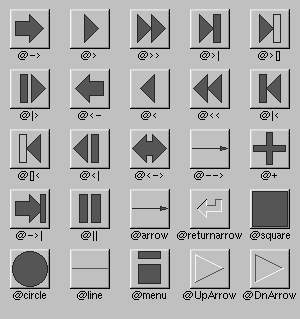
\includegraphics[scale=1]{symbols} 


 FLTK label supported symbols.


  The @ sign may be followed by the following optional ``formatting'' characters, in this order: 


 
\begin{enumerate}
\item 

 ``\#'' forces square scaling rather than distortion to the widget's shape.

\item 

 +[1-9] or -[1-9] tweaks the scaling a little bigger or smaller.

\item 

 [1-9] rotates by a multiple of 45 degrees. ``6'' does nothing, the others point in the direction of that key on a numeric keypad.


\end{enumerate}


 \emph{itype}
 -- an integer number denoting the appearance of the widget. 


  The following values are legal for \emph{itype}
: 


 
\begin{itemize}
\item 

 1 - flat box

\item 

 2 - up box

\item 

 3 - down box

\item 

 4 - thin up box

\item 

 5 - thin down box

\item 

 6 - engraved box

\item 

 7 - embossed box

\item 

 8 - border box

\item 

 9 - shadow box

\item 

 10 - rounded box

\item 

 11 - rounded box with shadow

\item 

 12 - rounded flat box

\item 

 13 - rounded up box

\item 

 14 - rounded down box

\item 

 15 - diamond up box

\item 

 16 - diamond down box

\item 

 17 - oval box

\item 

 18 - oval shadow box

\item 

 19 - oval flat box


\end{itemize}


 \emph{ifont}
 -- an integer number denoting the font of \emph{FLbox}
. 


 \emph{ifont}
 argument to set the font type. The following values are legal for \emph{ifont}
: 


 
\begin{itemize}
\item 

 1 - helvetica (same as ``Arial'' under Windows)

\item 

 2 - helvetica bold

\item 

 3 - helvetica italic

\item 

 4 - helvetica bold italic

\item 

 5 - courier

\item 

 6 - courier bold

\item 

 7 - courier italic

\item 

 8 - courier bold italic

\item 

 9 - times

\item 

 10 - times bold

\item 

 11 - times italic

\item 

 12 - times bold italic

\item 

 13 - symbol

\item 

 14 - screen

\item 

 15 - screen bold

\item 

 16 - dingbats


\end{itemize}


 \emph{isize}
 -- size of the font. 


 \emph{iwidth}
 -- width of widget. 


 \emph{iheight}
 -- height of widget. 


 \emph{ix}
 -- horizontal position of the upper left corner of the valuator, relative to the upper left corner of corresponding window. (Expressed in pixels.) 


 \emph{iy}
 -- vertical position of the upper left corner of the valuator, relative to the upper left corner of corresponding window. (Expressed in pixels.) 


 \emph{image}
 -- a handle referring to an eventual image opened with \emph{bmopen}
 opcode. If it is set, it allows a skin for that widget. 


 


\begin{tabular}{cc}
\textbf{Note about the bmopen opcode}
 \\
� &

  Although the documentation mentions the \emph{bmopen}
 opcode, it has not been implemented in Csound 4.22. 


\end{tabular}

\subsection*{Performance}


 \emph{FLbox}
 is useful to show some text in a window. The text is bounded by a box, whose aspect depends on \emph{itype}
 argument. 


  Note that \emph{FLbox}
 is not a valuator and its value is fixed. Its value cannot be modified. 
\subsection*{Examples}


  Here is an example of the flbox opcode. It uses the files \emph{flbox.orc}
 and \emph{flbox.sco}
. 


 \textbf{Example 1. Example of the flbox opcode.}

\begin{lstlisting}
/* flbox.orc */
sr = 44100
kr = 441
ksmps = 100
nchnls = 1

FLpanel "Text Box", 700, 400, 50, 50
    ; Box border type (7=embossed box)
    itype = 7
    ; Font type (10='Times Bold')
    ifont = 10
    ; Font size
    isize = 20 
    ; Width of the flbox
    iwidth = 400
    ; Height of the flbox
    iheight = 30
    ; Distance of the left edge of the flbox
    ; from the left edge of the panel
    ix = 150
    ; Distance of the upper edge of the flbox
    ; from the upper edge of the panel
    iy = 100

    ih3 FLbox "Use Text Boxes For Labelling", itype, ifont, isize, iwidth, iheight, ix, iy
; End of panel contents
FLpanelEnd
; Run the widget thread!
FLrun

instr 1
endin
/* flbox.orc */
        
\end{lstlisting}
\begin{lstlisting}
/* flbox.sco */
; Real-time performance for 1 hour.
f 0 3600
e
/* flbox.sco */
        
\end{lstlisting}
\subsection*{See Also}


 \emph{FLbutBank}
, \emph{FLbutton}
, \emph{FLprintk}
, \emph{FLprintk2}
, \emph{FLvalue}

\subsection*{Credits}


 Author: Gabriel Maldonado


 New in version 4.22


 Example written by Iain McCurdy, edited by Kevin Conder.
%\hline 


\begin{comment}
\begin{tabular}{lcr}
Previous &Home &Next \\
flashtxt &Up &FLbutBank

\end{tabular}


\end{document}
\end{comment}

\newpage
\begin{comment}
\documentclass[10pt]{article}
\usepackage{fullpage, graphicx, url}
\setlength{\parskip}{1ex}
\setlength{\parindent}{0ex}
\title{FLbutBank}
\begin{document}


\begin{tabular}{ccc}
The Alternative Csound Reference Manual & & \\
Previous & &Next

\end{tabular}

%\hline 
\end{comment}
\section{FLbutBank}
FLbutBank�--� A FLTK widget opcode that creates a bank of buttons. \subsection*{Description}


  A FLTK widget opcode that creates a bank of buttons. 
\subsection*{Syntax}


 kout, ihandle \textbf{FLbutBank}
 itype, inumx, inumy, iwidth, iheight, ix, iy, iopcode [, kp1] [, kp2] [, kp3] [, kp4] [, kp5] [....] [, kpN]
\subsection*{Initialization}


 \emph{ihandle}
 -- a handle value (an integer number) that unequivocally references a corresponding widget. This is used by other opcodes that modify a widget's properties (see \emph{Modifying FLTK Widget Appearance}
). It is automatically output by \emph{FLbutBank}
 and must not be set by the user label. (The user label is a double-quoted string containing some user-provided text placed near the widget.) 


 \emph{itype}
 -- an integer number denoting the appearance of the widget. Its meaning is different for different types of widget. 


 \emph{inumx}
 -- number of buttons in each row of the bank. 


 \emph{inumy}
 -- number of buttons in each column of the bank 


 \emph{ix}
 -- horizontal position of upper left corner of the valuator, relative to the upper left corner of corresponding window, expressed in pixels 


 \emph{iy}
 -- vertical position of upper left corner of the valuator, relative to the upper left corner of corresponding window, expressed in pixels 


 \emph{iopcode}
 -- score opcode type. You have to provide the ascii code of the letter corresponding to the score opcode. At present time only ``i'' (ascii code 105) score statements are supported. A zero value refers to a default value of ``i''. So both 0 and 105 activates the \emph{i}
 opcode. A value of -1 disables this opcode feature. 
\subsection*{Performance}


 \emph{kout}
 -- output value 


 \emph{kp1}
, \emph{kp2}
, ..., \emph{kpN}
 -- arguments of the activated instruments. 


  The \emph{FLbutBank}
 opcode creates a bank of buttons. For example, the following line: 


 
\begin{lstlisting}
gkButton,ihb1  FLbutBank  12, 8, 8, 380, 180, 50, 350, 0, 7, 0, 0, 5000, 6000
        
\end{lstlisting}


 
 will create the this bank: 

 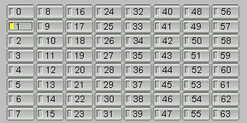
\includegraphics[scale=1]{flbutbank} 


 FLbutBank.


  A click to a button checks that button. It may also uncheck a previous checked button belonging to the same bank. So the behaviour is always that of radio-buttons. Notice that each button is labeled with a progressive number. The \emph{kout}
 argument is filled with that number when corresponding button is checked. 


 \emph{FLbutBank}
 not only outputs a value but can also activate (or schedule) an instrument provided by the user each time a button is pressed. If the \emph{iopcode}
 argument is set to a negative number, no instrument is activated so this feature is optional. In order to activate an instrument, \emph{iopcode}
 must be set to 0 or to 105 (the ascii code of character ``i'', referring to the \emph{i}
 score opcode). P-fields of the activated instrument are \emph{kp1}
 (instrument number), \emph{kp2}
 (action time), \emph{kp3}
 (duration) and so on with user p-fields. 


  The \emph{itype}
 argument sets the type of buttons identically to the \emph{FLbutton}
 opcode. By adding 10 to the \emph{itype}
 argument (i.e. by setting 11 for type 1, 12 for type 2, 13 for type 3 and 14 for type 4), it is possible to skip the current \emph{FLbutBank}
 value when getting/setting snapshots (see \emph{General FLTK Widget-related Opcodes}
). 


  FLbutBank is very useful to retrieve snapshots. 
\subsection*{See Also}


 \emph{FLbox}
, \emph{FLbutton}
, \emph{FLprintk}
, \emph{FLprintk2}
, \emph{FLvalue}

\subsection*{Credits}


 Author: Gabriel Maldonado


 New in version 4.22
%\hline 


\begin{comment}
\begin{tabular}{lcr}
Previous &Home &Next \\
FLbox &Up &FLbutton

\end{tabular}


\end{document}
\end{comment}

\newpage
\begin{comment}
\documentclass[10pt]{article}
\usepackage{fullpage, graphicx, url}
\setlength{\parskip}{1ex}
\setlength{\parindent}{0ex}
\title{FLbutton}
\begin{document}


\begin{tabular}{ccc}
The Alternative Csound Reference Manual & & \\
Previous & &Next

\end{tabular}

%\hline 
\end{comment}
\section{FLbutton}
FLbutton�--� A FLTK widget opcode that creates a button. \subsection*{Description}


  A FLTK widget opcode that creates a button. 
\subsection*{Syntax}


 kout, ihandle \textbf{FLbutton}
 ``label'', ion, ioff, itype, iwidth, iheight, ix, iy, iopcode [, kp1] [, kp2] [, kp3] [, kp4] [, kp5] [....] [, kpN]
\subsection*{Initialization}


 \emph{ihandle}
 -- a handle value (an integer number) that unequivocally references a corresponding widget. This is used by other opcodes that modify a widget's properties (see \emph{Modifying FLTK Widget Appearance}
). It is automatically output by \emph{FLbutton}
 and must not be set by the user label. (The user label is a double-quoted string containing some user-provided text placed near the widget.) 


 \emph{``label''}
 -- a double-quoted string containing some user-provided text, placed near the corresponding widget. 


  Notice that with \emph{FLbutton}
, it is not necessary to call the \emph{FLsetTextType}
 opcode at all in order to use a symbol. In this case, it is sufficient to set a label starting with ``@'' followed by the proper formatting string. 


  The following symbols are supported: 


 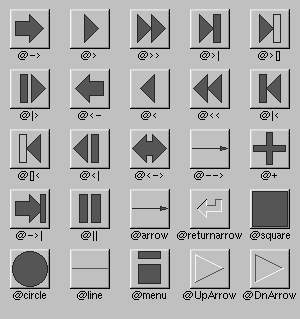
\includegraphics[scale=1]{symbols} 


 FLTK label supported symbols.


  The @ sign may be followed by the following optional ``formatting'' characters, in this order: 


 
\begin{enumerate}
\item 

 ``\#'' forces square scaling rather than distortion to the widget's shape.

\item 

 +[1-9] or -[1-9] tweaks the scaling a little bigger or smaller.

\item 

 [1-9] rotates by a multiple of 45 degrees. ``6'' does nothing, the others point in the direction of that key on a numeric keypad.


\end{enumerate}


 \emph{ion}
 -- value output when the button is checked. 


 \emph{ioff}
 -- value output when the button is unchecked. 


 \emph{itype}
 -- an integer number denoting the appearance of the widget. 


  Several kind of buttons are possible, according to the value of \emph{itype}
 argument: 


 
\begin{itemize}
\item 

 1 - normal button

\item 

 2 - light button

\item 

 3 - check button

\item 

 4 - round button


\end{itemize}


  This is the appearance of the buttons: 


 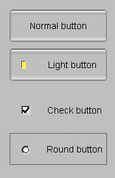
\includegraphics[scale=1]{flbutton} 


 FLbutton.


 \emph{iwidth}
 -- width of widget. 


 \emph{iheight}
 -- height of widget. 


 \emph{ix}
 -- horizontal position of upper left corner of the valuator, relative to the upper left corner of corresponding window (expressed in pixels). 


 \emph{iy}
 -- vertical position of upper left corner of the valuator, relative to the upper left corner of corresponding window (expressed in pixels). 


 \emph{iopcode}
 -- score opcode type. You have to provide the ascii code of the letter corresponding to the score opcode. At present time only ``i'' (ascii code 105) score statements are supported. A zero value refers to a default value of ``i''. So both 0 and 105 activates the \emph{i}
 opcode. A value of -1 disables this opcode feature. 
\subsection*{Performance}


 \emph{kout}
 -- output value 


 \emph{kp1}
, \emph{kp2}
, ..., \emph{kpN}
 -- arguments of the activated instruments. 


  Buttons of type 2, 3, and 4 also output (\emph{kout}
 argument) the value contained in the \emph{ion}
 argument when checked, and that contained in \emph{ioff}
 argument when unchecked. 


  By adding 10 to \emph{itype}
 argument (i.e. by setting 11 for type 1, 12 for type 2, 13 for type 3 and 14 for type 4) it is possible to skip the button value when getting/setting snapshots (see later section). \emph{FLbutton}
 not only outputs a value, but can also activate (or schedule) an instrument provided by the user each time a button is pressed. 


  If the \emph{iopcode}
 argument is set to a negative number, no instrument is activated. So this feature is optional. In order to activate an instrument, \emph{iopcode}
 must be set to 0 or to 105 (the ascii code of character ``i'', referring to the \emph{i}
 score opcode). 


  P-fields of the activated instrument are \emph{kp1}
 (instrument number), \emph{kp2}
 (action time), \emph{kp3}
 (duration) and so on with user p-fields. Notice that in dual state buttons (light button, check button and round button), the instrument is activated only when button state changes from unchecked to checked (not when passing from checked to unchecked). 
\subsection*{Examples}


  Here is an example of the flbutton opcode. It uses the files \emph{flbutton.orc}
, \emph{flbutton.sco}
, and \emph{beats.wav}
. 


 \textbf{Example 1. Example of the flbutton opcode.}

\begin{lstlisting}
/* flbutton.orc */
; Using fl-buttons to create on screen controls for play, 
; stop, fast forward and fast rewind of a sound file
; This example also makes use of a preset graphic for buttons.
sr = 44100
kr = 44100
ksmps = 1
nchnls = 1

FLpanel "Buttons", 320, 120, 100, 100
    ion = 0
    ioff = 0
    itype = 1
    iwidth = 50
    iheight = 50
    ix = 50
    iy = 35
    iopcode = 0
    istarttim = 0
    idur = -1

    ; Normal speed forwards
    gkplay, ihb1 FLbutton "@>", ion, ioff, itype, iwidth, iheight, ix, iy, iopcode, 1, istarttim, idur, 1 
    ; Stationary 
    gkstop, ihb2 FLbutton "@square", ion,ioff, itype, iwidth, iheight, ix+55, iy, iopcode, 1, istarttim, idur, 0
    ; Double speed backwards
    gkrew, ihb2 FLbutton "@<<", ion, ioff, itype, iwidth, iheight, ix+110, iy, iopcode, 1, istarttim, idur, -2
    ; Double speed forwardS
    gkff, ihb2 FLbutton "@>>", ion, ioff, itype, iwidth, iheight, ix+165, iy, iopcode, 1, istarttim, idur, 2
FLpanelEnd
FLrun

; Ensure that only 1 instance of instr 1
; plays even if the play button is clicked repeatedly
insnum = 1
icount = 1
maxalloc insnum, icount

instr 1
    asig diskin "beats.wav", p4, 0, 1
    out asig
endin
/* flbutton.orc */
        
\end{lstlisting}
\begin{lstlisting}
/* flbutton.sco */
; A sine wave
f 1 0 131072 10 1

; Real-time performance for 1 hour.
f 0 3600
e
/* flbutton.sco */
        
\end{lstlisting}
\subsection*{See Also}


 \emph{FLbox}
, \emph{FLbutBank}
, \emph{FLprintk}
, \emph{FLprintk2}
, \emph{FLvalue}

\subsection*{Credits}


 Author: Gabriel Maldonado


 New in version 4.22


 Example written by Iain McCurdy, edited by Kevin Conder.
%\hline 


\begin{comment}
\begin{tabular}{lcr}
Previous &Home &Next \\
FLbutBank &Up &FLcolor

\end{tabular}


\end{document}
\end{comment}

\newpage
\begin{comment}
\documentclass[10pt]{article}
\usepackage{fullpage, graphicx, url}
\setlength{\parskip}{1ex}
\setlength{\parindent}{0ex}
\title{FLcolor}
\begin{document}


\begin{tabular}{ccc}
The Alternative Csound Reference Manual & & \\
Previous & &Next

\end{tabular}

%\hline 
\end{comment}
\section{FLcolor}
FLcolor�--� A FLTK opcode that sets the primary colors. \subsection*{Description}


  Sets the primary colors to RGB values given by the user. 
\subsection*{Syntax}


 \textbf{FLcolor}
 ired, igreen, iblue
\subsection*{Initialization}


 \emph{ired}
 -- The red color of the target widget. The range for each RGB component is 0-255 


 \emph{igreen}
 -- The green color of the target widget. The range for each RGB component is 0-255 


 \emph{iblue}
 -- The blue color of the target widget. The range for each RGB component is 0-255 
\subsection*{Performance}


  These opcodes modify the appearance of other widgets. There are two types of such opcodes, those that don't contain the \emph{ihandle}
 argument which affect all subsequently declared widgets, and those without \emph{ihandle}
 which affect only a target widget previously defined. 


 \emph{FLcolor}
 sets the primary colors to RGB values given by the user. This opcode affects the primary color of (almost) all widgets defined next its location. User can put several instances of \emph{FLcolor}
 in front of each widget he intend to modify. However, to modify a single widget, it would be better to use the opcode belonging to the second type (i.e. those containing \emph{ihandle}
 argument). 


 \emph{FLcolor}
 is designed to modify the colors of a group of related widgets that assume the same color. The influence of \emph{FLcolor}
 on subsequent widgets can be turned off by using -1 as the only argument of the opcode. Also, using -2 (or -3) as the only value of \emph{FLcolor}
 makes all next widget colors randomly selected. The difference is that -2 selects a light random color, while -3 selects a dark random color. 
\subsection*{See Also}


 \emph{FLcolor2}
, \emph{FLhide}
, \emph{FLlabel}
, \emph{FLsetAlign}
, \emph{FLsetBox}
, \emph{FLsetColor}
, \emph{FLsetColor2}
, \emph{FLsetFont}
, \emph{FLsetPosition}
, \emph{FLsetSize}
, \emph{FLsetText}
, \emph{FLsetTextColor}
, \emph{FLsetTextSize}
, \emph{FLsetTextType}
, \emph{FLsetVal\_i}
, \emph{FLsetVal}
, \emph{FLshow}

\subsection*{Credits}


 Author: Gabriel Maldonado


 New in version 4.22
%\hline 


\begin{comment}
\begin{tabular}{lcr}
Previous &Home &Next \\
FLbutton &Up &FLcolor2

\end{tabular}


\end{document}
\end{comment}

\newpage
\begin{comment}
\documentclass[10pt]{article}
\usepackage{fullpage, graphicx, url}
\setlength{\parskip}{1ex}
\setlength{\parindent}{0ex}
\title{FLcolor2}
\begin{document}


\begin{tabular}{ccc}
The Alternative Csound Reference Manual & & \\
Previous & &Next

\end{tabular}

%\hline 
\end{comment}
\section{FLcolor2}
FLcolor2�--� A FLTK opcode that sets the secondary (selection) color. \subsection*{Description}


 \emph{FLcolor2}
 is the same of \emph{FLcolor}
 except it affects the secondary (selection) color. 
\subsection*{Syntax}


 \textbf{FLcolor2}
 ired, igreen, iblue
\subsection*{Initialization}


 \emph{ired}
 -- The red color of the target widget. The range for each RGB component is 0-255 


 \emph{igreen}
 -- The green color of the target widget. The range for each RGB component is 0-255 


 \emph{iblue}
 -- The blue color of the target widget. The range for each RGB component is 0-255 
\subsection*{Performance}


  These opcodes modify the appearance of other widgets. There are two types of such opcodes: those that don't contain the \emph{ihandle}
 argument which affect all subsequently declared widgets, and those without \emph{ihandle}
 which affect only a target widget previously defined. 


 \emph{FLcolor2}
 is the same of \emph{FLcolor}
 except it affects the secondary (selection) color. Setting it to -1 turns off the influence of \emph{FLcolor2}
 on subsequent widgets. A value of -2 (or -3) makes all next widget secondary colors randomly selected. The difference is that -2 selects a light random color, while -3 selects a dark random color. 
\subsection*{See Also}


 \emph{FLcolor}
, \emph{FLhide}
, \emph{FLlabel}
, \emph{FLsetAlign}
, \emph{FLsetBox}
, \emph{FLsetColor}
, \emph{FLsetColor2}
, \emph{FLsetFont}
, \emph{FLsetPosition}
, \emph{FLsetSize}
, \emph{FLsetText}
, \emph{FLsetTextColor}
, \emph{FLsetTextSize}
, \emph{FLsetTextType}
, \emph{FLsetVal\_i}
, \emph{FLsetVal}
, \emph{FLshow}

\subsection*{Credits}


 Author: Gabriel Maldonado


 New in version 4.22
%\hline 


\begin{comment}
\begin{tabular}{lcr}
Previous &Home &Next \\
FLcolor &Up &FLcount

\end{tabular}


\end{document}
\end{comment}

\newpage
\begin{comment}
\documentclass[10pt]{article}
\usepackage{fullpage, graphicx, url}
\setlength{\parskip}{1ex}
\setlength{\parindent}{0ex}
\title{FLcount}
\begin{document}


\begin{tabular}{ccc}
The Alternative Csound Reference Manual & & \\
Previous & &Next

\end{tabular}

%\hline 
\end{comment}
\section{FLcount}
FLcount�--� A FLTK widget opcode that creates a counter. \subsection*{Description}


  Allows the user to increase/decrease a value with mouse clicks on a corresponding arrow button. 
\subsection*{Syntax}


 kout, ihandle \textbf{FLcount}
 ``label'', imin, imax, istep1, istep2, itype, iwidth, iheight, ix, iy, iopcode [, kp1] [, kp2] [, kp3] [...] [, kpN]
\subsection*{Initialization}


 \emph{ihandle}
 -- a handle value (an integer number) that unequivocally references a corresponding widget. Used by further opcodes that changes some valuator's properties. It is automatically set by the corresponding valuator. 


 \emph{``label''}
 -- a double-quoted string containing some user-provided text, placed near the corresponding widget. 


 \emph{imin}
 -- minimum value of output range 


 \emph{imax}
 -- maximum value of output range 


 \emph{istep1}
 -- a floating-point number indicating the increment of valuator value corresponding to of each mouse click. \emph{istep1}
 is for coarse adjustments. 


 \emph{istep2}
 -- a floating-point number indicating the increment of valuator value corresponding to of each mouse click. \emph{istep2}
 is for fine adjustments. 


 \emph{itype}
 -- an integer number denoting the appearance of the valuator. 


 \emph{iwidth}
 -- width of widget. 


 \emph{iheight}
 -- height of widget. 


 \emph{ix}
 -- horizontal position of upper left corner of the valuator, relative to the upper left corner of corresponding window (expressed in pixels). 


 \emph{iy}
 -- vertical position of upper left corner of the valuator, relative to the upper left corner of corresponding window (expressed in pixels). 


 \emph{iopcode}
 -- score opcode type. You have to provide the ascii code of the letter corresponding to the score opcode. At present time only ``i'' (ascii code 105) score statements are supported. A zero value refers to a default value of ``i''. So both 0 and 105 activates the \emph{i}
 opcode. A value of -1 disables this opcode feature. 
\subsection*{Performance}


 \emph{kout}
 -- output value 


 \emph{kp1}
, \emph{kp2}
, ..., \emph{kpN}
 -- arguments of the activated instruments. 


 \emph{FLcount}
 allows the user to increase/decrease a value with mouse clicks on corresponding arrow buttons: 


 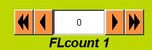
\includegraphics[scale=1]{flcount} 


 FLcount.


  There are two kind of arrow buttons, for larger and smaller steps. Notice that \emph{FLcount}
 not only outputs a value and a handle, but can also activate (schedule) an instrument provided by the user each time a button is pressed. P-fields of the activated instrument are \emph{kp1}
 (instrument number), \emph{kp2}
 (action time), \emph{kp3}
 (duration) and so on with user p-fields. If the \emph{iopcode}
 argument is set to a negative number, no instrument is activated. So this feature is optional. 
\subsection*{Examples}


  Here is an example of the flcount opcode. It uses the files \emph{flcount.orc}
 and \emph{flcount.sco}
. 


 \textbf{Example 1. Example of the flcount opcode.}

\begin{lstlisting}
/* flcount.orc */
; Demonstration of the flcount opcode
; clicking on the single arrow buttons
; increments the oscillator in semitone steps
; clicking on the double arrow buttons 
; increments the oscillator in octave steps
sr = 44100
kr = 441
ksmps = 100
nchnls = 1

FLpanel "Counter", 900, 400, 50, 50
    ; Minimum value output by counter
    imin = 6
    ; Maximum value output by counter
    imax = 12
    ; Single arrow step size (semitones)
    istep1 = 1/12
    ; Double arrow step size (octave)
    istep2 = 1 
    ; Counter type (1=double arrow counter)
    itype = 1
    ; Width of the counter in pixels
    iwidth = 200
    ; Height of the counter in pixels
    iheight = 30
    ; Distance of the left edge of the counter
    ; from the left edge of the panel
    ix = 50
    ; Distance of the top edge of the counter
    ; from the top edge of the panel
    iy = 50
    ; Score event type (-1=ignored)
    iopcode = -1

    gkoct, ihandle FLcount "pitch in oct format", imin, imax, istep1, istep2, itype, iwidth, iheight, ix, iy, iopcode, 1, 0, 1
; End of panel contents
FLpanelEnd
; Run the widget thread!
FLrun

instr 1
    iamp = 15000
    ifn = 1
    asig oscili iamp, cpsoct(gkoct), ifn
    out asig
endin
/* flcount.orc */
        
\end{lstlisting}
\begin{lstlisting}
/* flcount.sco */
; Function table that defines a single cycle
; of a sine wave.
f 1 0 1024 10 1

; Instrument 1 will play a note for 1 hour.
i 1 0 3600
e
/* flcount.sco */
        
\end{lstlisting}
\subsection*{See Also}


 \emph{FLjoy}
, \emph{FLkeyb}
, \emph{FLknob}
, \emph{FLroller}
, \emph{FLslider}
, \emph{FLtext}

\subsection*{Credits}


 Author: Gabriel Maldonado


 New in version 4.22


 Example written by Iain McCurdy, edited by Kevin Conder.
%\hline 


\begin{comment}
\begin{tabular}{lcr}
Previous &Home &Next \\
FLcolor2 &Up &FLgetsnap

\end{tabular}


\end{document}
\end{comment}

\newpage
\begin{comment}
\documentclass[10pt]{article}
\usepackage{fullpage, graphicx, url}
\setlength{\parskip}{1ex}
\setlength{\parindent}{0ex}
\title{FLgetsnap}
\begin{document}


\begin{tabular}{ccc}
The Alternative Csound Reference Manual & & \\
Previous & &Next

\end{tabular}

%\hline 
\end{comment}
\section{FLgetsnap}
FLgetsnap�--� Retrieves a previously stored FLTK snapshot. \subsection*{Description}


  Retrieves a previously stored snapshot (in memory), i.e. sets all valuator to the corresponding values stored in that snaphot. 
\subsection*{Syntax}


 inumsnap \textbf{FLgetsnap}
 index
\subsection*{Initialization}


 \emph{inumsnap}
 -- current number of snapshots. 


 \emph{index}
 -- a number referring unequivocally to a snapshot. Several snapshots can be stored in the same bank. 
\subsection*{Performance}


 \emph{FLgetsnap}
 retrieves a previously stored snapshot (in memory), i.e. sets all valuator to the corresponding values stored in that snapshot. The \emph{index}
 argument unequivocally must refer to an already existing snapshot. If the \emph{index}
 argument refers to an empty snapshot or to a snapshot that doesn't exist, no action is done. \emph{FLsetsnap}
 outputs the current number of snapshots (\emph{inumsnap}
 argument). 
\subsection*{See Also}


 \emph{FLloadsnap}
, \emph{FLrun}
, \emph{FLsavesnap}
, \emph{FLsetsnap}
, \emph{FLupdate}

\subsection*{Credits}


 Author: Gabriel Maldonado


 New in version 4.22
%\hline 


\begin{comment}
\begin{tabular}{lcr}
Previous &Home &Next \\
FLcount &Up &FLgroup

\end{tabular}


\end{document}
\end{comment}

\newpage
\begin{comment}
\documentclass[10pt]{article}
\usepackage{fullpage, graphicx, url}
\setlength{\parskip}{1ex}
\setlength{\parindent}{0ex}
\title{FLgroup}
\begin{document}


\begin{tabular}{ccc}
The Alternative Csound Reference Manual & & \\
Previous & &Next

\end{tabular}

%\hline 
\end{comment}
\section{FLgroup}
FLgroup�--� A FLTK container opcode that groups child widgets. \subsection*{Description}


  A FLTK container opcode that groups child widgets. 
\subsection*{Syntax}


 \textbf{FLgroup}
 ``label'', iwidth, iheight, ix, iy [, iborder] [, image]
\subsection*{Initialization}


 \emph{``label''}
 -- a double-quoted string containing some user-provided text, placed near the corresponding widget. 


 \emph{iwidth}
 -- width of widget. 


 \emph{iheight}
 -- height of widget. 


 \emph{ix}
 -- horizontal position of upper left corner of the valuator, relative to the upper left corner of corresponding window (expressed in pixels). 


 \emph{iy}
 -- vertical position of upper left corner of the valuator, relative to the upper left corner of corresponding window (expressed in pixels). 


 \emph{iborder}
 (optional, default=0) -- border type of the container. It is expressed by means of an integer number chosen from the following: 


 
\begin{itemize}
\item 

 0 - no border

\item 

 1 - down box border

\item 

 2 - up box border

\item 

 3 - engraved border

\item 

 4 - embossed border

\item 

 5 - black line border

\item 

 6 - thin down border

\item 

 7 - thin up border


\end{itemize}
 If the integer number doesn't match any of the previous values, no border is provided as the default. 

 \emph{image}
 (optional) -- a handle referring to an eventual image opened with the \emph{bmopen}
 opcode. If it is set, it allows a skin for that widget. 


 


\begin{tabular}{cc}
\textbf{Note about the bmopen opcode}
 \\
� &

  Although the documentation mentions the \emph{bmopen}
 opcode, it has not been implemented in Csound 4.22. 


\end{tabular}

\subsection*{Performance}


  Containers are useful to format the graphic appearance of the widgets. The most important container is \emph{FLpanel}
, that actually creates a window. It can be filled with other containers and/or valuators or other kinds of widgets. 


  There are no k-rate arguments in containers. 
\subsection*{See Also}


 \emph{FLgroupEnd}
, \emph{FLpack}
, \emph{FLpackEnd}
, \emph{FLpanel}
, \emph{FLpanelEnd}
, \emph{FLscroll}
, \emph{FLscrollEnd}
, \emph{FLtabs}
, \emph{FLtabsEnd}

\subsection*{Credits}


 Author: Gabriel Maldonado


 New in version 4.22
%\hline 


\begin{comment}
\begin{tabular}{lcr}
Previous &Home &Next \\
FLgetsnap &Up &FLgroupEnd

\end{tabular}


\end{document}
\end{comment}

\newpage
\begin{comment}
\documentclass[10pt]{article}
\usepackage{fullpage, graphicx, url}
\setlength{\parskip}{1ex}
\setlength{\parindent}{0ex}
\title{FLgroupEnd}
\begin{document}


\begin{tabular}{ccc}
The Alternative Csound Reference Manual & & \\
Previous & &Next

\end{tabular}

%\hline 
\end{comment}
\section{FLgroupEnd}
FLgroupEnd�--� Marks the end of a group of FLTK child widgets. \subsection*{Description}


  Marks the end of a group of FLTK child widgets. 
\subsection*{Syntax}


 \textbf{FLgroupEnd}

\subsection*{Performance}


  Containers are useful to format the graphic appearance of the widgets. The most important container is \emph{FLpanel}
, that actually creates a window. It can be filled with other containers and/or valuators or other kinds of widgets. 


  There are no k-rate arguments in containers. 
\subsection*{See Also}


 \emph{FLgroup}
, \emph{FLpack}
, \emph{FLpackEnd}
, \emph{FLpanel}
, \emph{FLpanelEnd}
, \emph{FLscroll}
, \emph{FLscrollEnd}
, \emph{FLtabs}
, \emph{FLtabsEnd}

\subsection*{Credits}


 Author: Gabriel Maldonado


 New in version 4.22
%\hline 


\begin{comment}
\begin{tabular}{lcr}
Previous &Home &Next \\
FLgroup &Up &FLhide

\end{tabular}


\end{document}
\end{comment}

\newpage
\begin{comment}
\documentclass[10pt]{article}
\usepackage{fullpage, graphicx, url}
\setlength{\parskip}{1ex}
\setlength{\parindent}{0ex}
\title{FLhide}
\begin{document}


\begin{tabular}{ccc}
The Alternative Csound Reference Manual & & \\
Previous & &Next

\end{tabular}

%\hline 
\end{comment}
\section{FLhide}
FLhide�--� Hides the target FLTK widget. \subsection*{Description}


  Hides the target FLTK widget, making it invisible. 
\subsection*{Syntax}


 \textbf{FLhide}
 ihandle
\subsection*{Initialization}


 \emph{ihandle}
 -- a handle value (an integer number) that unequivocally references a corresponding widget. This is used by other opcodes that modify a widget's properties (see \emph{Modifying FLTK Widget Appearance}
). It is automatically output by \emph{FLbutBank}
 and must not be set by the user label. (The user label is a double-quoted string containing some user-provided text placed near the widget.) 
\subsection*{Performance}


 \emph{FLhide}
 hides target widget, making it invisible. 
\subsection*{See Also}


 \emph{FLcolor}
, \emph{FLcolor2}
, \emph{FLlabel}
, \emph{FLsetAlign}
, \emph{FLsetBox}
, \emph{FLsetColor}
, \emph{FLsetColor2}
, \emph{FLsetFont}
, \emph{FLsetPosition}
, \emph{FLsetSize}
, \emph{FLsetText}
, \emph{FLsetTextColor}
, \emph{FLsetTextSize}
, \emph{FLsetTextType}
, \emph{FLsetVal\_i}
, \emph{FLsetVal}
, \emph{FLshow}

\subsection*{Credits}


 Author: Gabriel Maldonado


 New in version 4.22
%\hline 


\begin{comment}
\begin{tabular}{lcr}
Previous &Home &Next \\
FLgroupEnd &Up &FLjoy

\end{tabular}


\end{document}
\end{comment}

\newpage
\begin{comment}
\documentclass[10pt]{article}
\usepackage{fullpage, graphicx, url}
\setlength{\parskip}{1ex}
\setlength{\parindent}{0ex}
\title{FLjoy}
\begin{document}


\begin{tabular}{ccc}
The Alternative Csound Reference Manual & & \\
Previous & &Next

\end{tabular}

%\hline 
\end{comment}
\section{FLjoy}
FLjoy�--� A FLTK opcode that acts like a joystick. \subsection*{Description}


 \emph{FLjoy}
 is a squared area that allows the user to modify two output values at the same time. It acts like a joystick. 
\subsection*{Syntax}


 koutx, kouty, ihandlex, ihandley \textbf{FLjoy}
 ``label'', iminx, imaxx, iminy, imaxy, iexpx, iexpy, idispx, idispy, iwidth, iheight, ix, iy
\subsection*{Initialization}


 \emph{ihandlex}
 -- a handle value (an integer number) that unequivocally references a corresponding widget. Used by further opcodes that changes some valuator's properties. It is automatically set by the corresponding valuator. 


 \emph{ihandley}
 -- a handle value (an integer number) that unequivocally references a corresponding widget. Used by further opcodes that changes some valuator's properties. It is automatically set by the corresponding valuator. 


 \emph{``label''}
 -- a double-quoted string containing some user-provided text, placed near the corresponding widget. 


 \emph{iminx}
 -- minimum x value of output range 


 \emph{imaxx}
 -- maximum x value of output range 


 \emph{iminy}
 -- minimum y value of output range 


 \emph{imaxy}
 -- maximum y value of output range 


 \emph{iwidth}
 -- width of widget. 


 \emph{idispx}
 -- a handle value that was output from a previous instance of the \emph{FLvalue}
 opcode to display the current value of the current valuator in the \emph{FLvalue}
 widget itself. If the user doesn't want to use this feature that displays current values, it must be set to a negative number by the user. 


 \emph{idispy}
 -- a handle value that was output from a previous instance of the \emph{FLvalue}
 opcode to display the current value of the current valuator in the \emph{FLvalue}
 widget itself. If the user doesn't want to use this feature that displays current values, it must be set to a negative number by the user. 


 \emph{iexpx}
 -- an integer number denoting the behaviour of valuator: 


 
\begin{itemize}
\item 

 0 = valuator output is linear

\item 

 -1 = valuator output is exponential


\end{itemize}


  All other positive numbers for \emph{iexpx}
 indicate the number of an existing table that is used for indexing. Linear interpolation is provided in table indexing. A negative table number suppresses interpolation. 


 \emph{iexpy}
 -- an integer number denoting the behaviour of valuator: 


 
\begin{itemize}
\item 

 0 = valuator output is linear

\item 

 -1 = valuator output is exponential


\end{itemize}


  All other positive numbers for \emph{iexpy}
 indicate the number of an existing table that is used for indexing. Linear interpolation is provided in table indexing. A negative table number suppresses interpolation. 


 


\begin{tabular}{cc}
Warning &\textbf{IMPORTANT!}
 \\
� &

  Notice that the tables used by valuators must be created with the \emph{ftgen}
 opcode and placed in the orchestra before the corresponding valuator. They can not placed in the score. In fact, tables placed in the score are created later than the initialization of the opcodes placed in the header section of the orchestra. 


\end{tabular}



 \emph{iheight}
 -- height of widget. 


 \emph{ix}
 -- horizontal position of upper left corner of the valuator, relative to the upper left corner of corresponding window (expressed in pixels). 


 \emph{iy}
 -- vertical position of upper left corner of the valuator, relative to the upper left corner of corresponding window (expressed in pixels). 
\subsection*{Performance}


 \emph{koutx}
 -- x output value 


 \emph{kouty}
 -- y output value 
\subsection*{Examples}


  Here is an example of the fljoy opcode. It uses the files \emph{fljoy.orc}
 and \emph{fljoy.sco}
. 


 \textbf{Example 1. Example of the fljoy opcode.}

\begin{lstlisting}
/* fljoy.orc */
; Demonstration of the flpanel opcode
; Horizontal click-dragging controls the frequency of the oscillator
; Vertical click-dragging controls the amplitude of the oscillator
sr = 44100
kr = 441
ksmps = 100
nchnls = 1

FLpanel "X Y Panel", 900, 400, 50, 50
    ; Minimum value output by x movement (frequency)
    iminx = 200
    ; Maximum value output by x movement (frequency)
    imaxx = 5000 
    ; Minimum value output by y movement (amplitude)
    iminy = 0
    ; Maximum value output by y movement (amplitude)
    imaxy = 15000
    ; Logarithmic change in x direction
    iexpx = -1
    ; Linear change in y direction
    iexpy = 0
    ; Display handle x direction (-1=not used)
    idispx = -1
    ; Display handle y direction (-1=not used)
    idispy = -1
    ; Width of the x y panel in pixels
    iwidth = 800
    ; Height of the x y panel in pixels
    iheight = 300
    ; Distance of the left edge of the x y panel from 
    ; the left edge of the panel
    ix = 50
    ; Distance of the top edge of the x y 
    ; panel from the top edge of the panel
    iy = 50

    gkfreqx, gkampy, ihandlex, ihandley FLjoy "X - Frequency Y - Amplitude", iminx, imaxx, iminy, imaxy, iexpx, iexpy, idispx, idispy, iwidth, iheight, ix, iy
; End of panel contents
FLpanelEnd
; Run the widget thread!
FLrun

instr 1
    ifn = 1
    asig oscili gkampy, gkfreqx, ifn
    out asig
endin
/* fljoy.orc */
        
\end{lstlisting}
\begin{lstlisting}
/* fljoy.sco */
; Function table that defines a single cycle
; of a sine wave.
f 1 0 1024 10 1

; Instrument 1 will play a note for 1 hour.
i 1 0 3600
e
/* fljoy.sco */
        
\end{lstlisting}
\subsection*{See Also}


 \emph{FLcount}
, \emph{FLkeyb}
, \emph{FLknob}
, \emph{FLroller}
, \emph{FLslider}
, \emph{FLtext}

\subsection*{Credits}


 Author: Gabriel Maldonado


 New in version 4.22


 Example written by Iain McCurdy, edited by Kevin Conder.
%\hline 


\begin{comment}
\begin{tabular}{lcr}
Previous &Home &Next \\
FLhide &Up &FLkeyb

\end{tabular}


\end{document}
\end{comment}

\newpage
\begin{comment}
\documentclass[10pt]{article}
\usepackage{fullpage, graphicx, url}
\setlength{\parskip}{1ex}
\setlength{\parindent}{0ex}
\title{FLkeyb}
\begin{document}


\begin{tabular}{ccc}
The Alternative Csound Reference Manual & & \\
Previous & &Next

\end{tabular}

%\hline 
\end{comment}
\section{FLkeyb}
FLkeyb�--� Experimental, no documentation exists. May be deprecated in future versions. \subsection*{Description}


  Experimental, no documentation exists. May be deprecated in future versions. 
\subsection*{Syntax}


 kout \textbf{FLkeyb}
 kparam1 [, kparam2] ... [, kparamN]
\subsection*{See Also}


 \emph{FLcount}
, \emph{FLjoy}
, \emph{FLknob}
, \emph{FLroller}
, \emph{FLslider}
, \emph{FLtext}

\subsection*{Credits}


 Author: Gabriel Maldonado


 New in version 4.22
%\hline 


\begin{comment}
\begin{tabular}{lcr}
Previous &Home &Next \\
FLjoy &Up &FLknob

\end{tabular}


\end{document}
\end{comment}

\newpage
\begin{comment}
\documentclass[10pt]{article}
\usepackage{fullpage, graphicx, url}
\setlength{\parskip}{1ex}
\setlength{\parindent}{0ex}
\title{FLknob}
\begin{document}


\begin{tabular}{ccc}
The Alternative Csound Reference Manual & & \\
Previous & &Next

\end{tabular}

%\hline 
\end{comment}
\section{FLknob}
FLknob�--� A FLTK widget opcode that creates a knob. \subsection*{Description}


  A FLTK widget opcode that creates a knob. 
\subsection*{Syntax}


 kout, ihandle \textbf{FLknob}
 ``label'', imin, imax, iexp, itype, idisp, iwidth, ix, iy [, icursorsize]
\subsection*{Initialization}


 \emph{ihandle}
 -- a handle value (an integer number) that unequivocally references a corresponding widget. This is used by other opcodes that modify a widget's properties (see \emph{Modifying FLTK Widget Appearance}
). It is automatically output by \emph{FLknob}
 and must not be set by the user label. (The user label is a double-quoted string containing some user-provided text placed near the widget.) 


 \emph{``label''}
 -- a double-quoted string containing some user-provided text, placed near the corresponding widget. 


 \emph{imin}
 -- minimum value of output range. 


 \emph{imax}
 -- maximum value of output range. 


 \emph{iexp}
 -- an integer number denoting the behaviour of valuator: 


 
\begin{itemize}
\item 

 0 = valuator output is linear

\item 

 -1 = valuator output is exponential


\end{itemize}


  All other positive numbers for \emph{iexp}
 indicate the number of an existing table that is used for indexing. Linear interpolation is provided in table indexing. A negative table number suppresses interpolation. 


 


\begin{tabular}{cc}
Warning &\textbf{IMPORTANT!}
 \\
� &

  Notice that the tables used by valuators must be created with the \emph{ftgen}
 opcode and placed in the orchestra before the corresponding valuator. They can not placed in the score. In fact, tables placed in the score are created later than the initialization of the opcodes placed in the header section of the orchestra. 


\end{tabular}



 \emph{itype}
 -- an integer number denoting the appearance of the valuator. 


  The \emph{itype}
 argument can be set to the following values: 


 
\begin{itemize}
\item 

 1 - a 3-D knob

\item 

 2 - a pie-like knob

\item 

 3 - a clock-like knob

\item 

 4 - a flat knob


\end{itemize}


 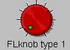
\includegraphics[scale=1]{flknob_3d} 


 A 3-D knob.


 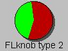
\includegraphics[scale=1]{flknob_pie} 


 A pie knob.


 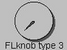
\includegraphics[scale=1]{flknob_clock} 


 A clock knob.


 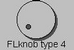
\includegraphics[scale=1]{flknob_flat} 


 A flat knob.


 \emph{idisp}
 -- a handle value that was output from a previous instance of the \emph{FLvalue}
 opcode to display the current value of the current valuator in the \emph{FLvalue}
 widget itself. If the user doesn't want to use this feature that displays current values, it must be set to a negative number by the user. 


 \emph{iwidth}
 -- width of widget. 


 \emph{iheight}
 -- height of widget. 


 \emph{ix}
 -- horizontal position of upper left corner of the valuator, relative to the upper left corner of corresponding window (expressed in pixels). 


 \emph{iy}
 -- vertical position of upper left corner of the valuator, relative to the upper left corner of corresponding window (expressed in pixels). 


 \emph{icursorsize}
 (optional) -- If \emph{FLknob}
's \emph{itype}
 is set to 1 (3D knob), this parameter controls the size of knob cursor. 
\subsection*{Performance}


 \emph{kout}
 -- output value 


 \emph{FLknob}
 puts a knob in the corresponding container. 
\subsection*{Examples}


  Here is an example of the FLknob opcode. It uses the files \emph{flknob.orc}
 and \emph{flknob.sco}
. 


 \textbf{Example 1. Example of the FLknob opcode.}

\begin{lstlisting}
/* flknob.orc */
; A sine with oscillator with flknob controlled frequency
sr = 44100
kr = 441
ksmps = 100
nchnls = 1

FLpanel "Frequency Knob", 900, 400, 50, 50
    ; Minimum value output by the knob
    imin = 200
    ; Maximum value output by the knob
    imax = 5000
    ; Logarithmic type knob selected
    iexp = -1
    ; Knob graphic type (1=3D knob)
    itype = 1 
    ; Display handle (-1=not used)
    idisp = -1
    ; Width of the knob in pixels
    iwidth = 70
    ; Height of the knob in pixels
    iheight = 70
    ; Distance of the left edge of the knob 
    ; from the left edge of the panel
    ix = 125

    gkfreq, ihandle FLknob "Frequency", imin, imax, iexp, itype, idisp, iwidth, iheight, ix
; End of panel contents
FLpanelEnd
; Run the widget thread!
FLrun

instr 1
    iamp = 15000
    ifn = 1
    asig oscili iamp, gkfreq, ifn
    out asig
endin
/* flknob.orc */
        
\end{lstlisting}
\begin{lstlisting}
/* flknob.sco */
; Function table that defines a single cycle
; of a sine wave.
f 1 0 1024 10 1

; Instrument 1 will play a note for 1 hour.
i 1 0 3600
e
/* flknob.sco */
        
\end{lstlisting}
\subsection*{See Also}


 \emph{FLcount}
, \emph{FLjoy}
, \emph{FLkeyb}
, \emph{FLroller}
, \emph{FLslider}
, \emph{FLtext}

\subsection*{Credits}


 Author: Gabriel Maldonado


 New in version 4.22


 Example written by Iain McCurdy, edited by Kevin Conder.
%\hline 


\begin{comment}
\begin{tabular}{lcr}
Previous &Home &Next \\
FLkeyb &Up &FLlabel

\end{tabular}


\end{document}
\end{comment}

\newpage
\begin{comment}
\documentclass[10pt]{article}
\usepackage{fullpage, graphicx, url}
\setlength{\parskip}{1ex}
\setlength{\parindent}{0ex}
\title{FLlabel}
\begin{document}


\begin{tabular}{ccc}
The Alternative Csound Reference Manual & & \\
Previous & &Next

\end{tabular}

%\hline 
\end{comment}
\section{FLlabel}
FLlabel�--� A FLTK opcode that modifies the appearance of a text label. \subsection*{Description}


  Modifies a set of parameters related to the text label appearence of a widget (i.e. size, font, alignment and color of corresponding text). 
\subsection*{Syntax}


 \textbf{FLlabel}
 isize, ifont, ialign, ired, igreen, iblue
\subsection*{Initialization}


 \emph{isize}
 -- size of the font of the target widget. Normal values are in the order of 15. Greater numbers enlarge font size, while smaller numbers reduce it. 


 \emph{ifont}
 -- sets the the font type of the label of a widget. 


  Legal values for ifont argument are: 


 
\begin{itemize}
\item 

 1 - Helvetica (same as Arial under Windows)

\item 

 2 - Helvetica Bold

\item 

 3 - Helvetica Italic

\item 

 4 - Helvetica Bold Italic

\item 

 5 - Courier

\item 

 6 - Courier Bold

\item 

 7 - Courier Italic

\item 

 8 - Courier Bold Italic

\item 

 9 - Times

\item 

 10 - Times Bold

\item 

 11 - Times Italic

\item 

 12 - Times Bold Italic

\item 

 13 - Symbol

\item 

 14 - Screen

\item 

 15 - Screen Bold

\item 

 16 - Dingbats


\end{itemize}


 \emph{ialign}
 -- sets the alignment of the label text of the widget. 


  Legal values for ialign argument are: 


 
\begin{itemize}
\item 

 1 - align center

\item 

 2 - align top

\item 

 3 - align bottom

\item 

 4 - align left

\item 

 5 - align right

\item 

 6 - align top-left

\item 

 7 - align top-right

\item 

 8 - align bottom-left

\item 

 9 - align bottom-right


\end{itemize}


 \emph{ired}
 -- The red color of the target widget. The range for each RGB component is 0-255 


 \emph{igreen}
 -- The green color of the target widget. The range for each RGB component is 0-255 


 \emph{iblue}
 -- The blue color of the target widget. The range for each RGB component is 0-255 
\subsection*{Performance}


 \emph{FLlabel}
 modifies a set of parameters related to the text label appearance of a widget, i.e. size, font, alignment and color of corresponding text. This opcode affects (almost) all widgets defined next its location. A user can put several instances of \emph{FLlabel}
 in front of each widget he intends to modify. However, to modify a particular widget, it is better to use the opcode belonging to the second type (i.e. those containing the \emph{ihandle}
 argument). 


  The influence of \emph{FLlabel}
 on the next widget can be turned off by using -1 as its only argument. \emph{FLlabel}
 is designed to modify text attributes of a group of related widgets. 
\subsection*{See Also}


 \emph{FLcolor}
, \emph{FLcolor2}
, \emph{FLhide}
, \emph{FLsetAlign}
, \emph{FLsetBox}
, \emph{FLsetColor}
, \emph{FLsetColor2}
, \emph{FLsetFont}
, \emph{FLsetPosition}
, \emph{FLsetSize}
, \emph{FLsetText}
, \emph{FLsetTextColor}
, \emph{FLsetTextSize}
, \emph{FLsetTextType}
, \emph{FLsetVal\_i}
, \emph{FLsetVal}
, \emph{FLshow}

\subsection*{Credits}


 Author: Gabriel Maldonado


 New in version 4.22
%\hline 


\begin{comment}
\begin{tabular}{lcr}
Previous &Home &Next \\
FLknob &Up &FLloadsnap

\end{tabular}


\end{document}
\end{comment}

\newpage
\begin{comment}
\documentclass[10pt]{article}
\usepackage{fullpage, graphicx, url}
\setlength{\parskip}{1ex}
\setlength{\parindent}{0ex}
\title{FLloadsnap}
\begin{document}


\begin{tabular}{ccc}
The Alternative Csound Reference Manual & & \\
Previous & &Next

\end{tabular}

%\hline 
\end{comment}
\section{FLloadsnap}
FLloadsnap�--� Loads all snapshots into the memory bank of the current orchestra. \subsection*{Description}


 \emph{FLloadsnap}
 loads all the snapshots contained in a file into the memory bank of the current orchestra. 
\subsection*{Syntax}


 \textbf{FLloadsnap}
 ``filename''
\subsection*{Initialization}


 \emph{``filename''}
 -- a double-quoted string corresponding to a file to load a bank of snapshots. 
\subsection*{Performance}


 \emph{FLloadsnap}
 loads all snapshots contained in filename into the memory bank of current orchestra. 
\subsection*{See Also}


 \emph{FLgetsnap}
, \emph{FLrun}
, \emph{FLsavesnap}
, \emph{FLsetsnap}
, \emph{FLupdate}

\subsection*{Credits}


 Author: Gabriel Maldonado


 New in version 4.22
%\hline 


\begin{comment}
\begin{tabular}{lcr}
Previous &Home &Next \\
FLlabel &Up &FLpack

\end{tabular}


\end{document}
\end{comment}

\newpage
\begin{comment}
\documentclass[10pt]{article}
\usepackage{fullpage, graphicx, url}
\setlength{\parskip}{1ex}
\setlength{\parindent}{0ex}
\title{FLpack}
\begin{document}


\begin{tabular}{ccc}
The Alternative Csound Reference Manual & & \\
Previous & &Next

\end{tabular}

%\hline 
\end{comment}
\section{FLpack}
FLpack�--� Provides the functionality of compressing and aligning FLTK widgets. \subsection*{Description}


 \emph{FLpack}
 provides the functionality of compressing and aligning widgets. 
\subsection*{Syntax}


 \textbf{FLpack}
 iwidth, iheight, ix, iy, itype, ispace, iborder
\subsection*{Initialization}


 \emph{iwidth}
 -- width of widget. 


 \emph{iheight}
 -- height of widget. 


 \emph{ix}
 -- horizontal position of upper left corner of the valuator, relative to the upper left corner of corresponding window (expressed in pixels). 


 \emph{iy}
 -- vertical position of upper left corner of the valuator, relative to the upper left corner of corresponding window (expressed in pixels). 


 \emph{itype}
 -- an integer number that modifies the appearance of the target widget. 


  The \emph{itype}
 argument expresses the type of packing: 


 
\begin{itemize}
\item 

 0 - vertical

\item 

 1 - horizontal


\end{itemize}


 \emph{ispace}
 -- sets the space between the widgets. 


 \emph{iborder}
 -- border type of the container. It is expressed by means of an integer number chosen from the following: 


 
\begin{itemize}
\item 

 0 - no border

\item 

 1 - down box border

\item 

 2 - up box border

\item 

 3 - engraved border

\item 

 4 - embossed border

\item 

 5 - black line border

\item 

 6 - thin down border

\item 

 7 - thin up border


\end{itemize}
\subsection*{Performance}


 \emph{FLpack}
 provides the functionality of compressing and aligning widgets. 


  Containers are useful to format the graphic appearance of the widgets. The most important container is \emph{FLpanel}
, that actually creates a window. It can be filled with other containers and/or valuators or other kinds of widgets. 


  There are no k-rate arguments in containers. 
\subsection*{Examples}


  The following example: 


 
\begin{lstlisting}
        FLpanel "Panel1",450,300,100,100
        FLpack  400,300, 10,40,0,15,3
gk1,ihs1        FLslider        "FLslider 1", 500, 1000, 2 ,1, -1, 300,15, 20,50
gk2,ihs2        FLslider        "FLslider 2", 300, 5000, 2 ,3, -1, 300,15, 20,100
gk3,ihs3        FLslider        "FLslider 3", 350, 1000, 2 ,5, -1, 300,15, 20,150
gk4,ihs4        FLslider        "FLslider 4", 250, 5000, 1 ,11, -1, 300,30, 20,200
gk5,ihs5        FLslider        "FLslider 5", 220, 8000, 2 ,1, -1, 300,15, 20,250
gk6,ihs6        FLslider        "FLslider 6", 1, 5000, 1 ,13, -1, 300,15, 20,300
gk7,ihs7        FLslider        "FLslider 7", 870, 5000, 1 ,15, -1, 300,30, 20,350
        FLpackEnd
        FLpanelEnd
        
\end{lstlisting}


 
 ...will produce this result, when resizing the window: 

 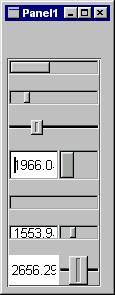
\includegraphics[scale=1]{flpack} 


 FLpack.
\subsection*{See Also}


 \emph{FLgroup}
, \emph{FLgroupEnd}
, \emph{FLpackEnd}
, \emph{FLpanel}
, \emph{FLpanelEnd}
, \emph{FLscroll}
, \emph{FLscrollEnd}
, \emph{FLtabs}
, \emph{FLtabsEnd}

\subsection*{Credits}


 Author: Gabriel Maldonado


 New in version 4.22
%\hline 


\begin{comment}
\begin{tabular}{lcr}
Previous &Home &Next \\
FLloadsnap &Up &FLpackEnd

\end{tabular}


\end{document}
\end{comment}

\newpage
\begin{comment}
\documentclass[10pt]{article}
\usepackage{fullpage, graphicx, url}
\setlength{\parskip}{1ex}
\setlength{\parindent}{0ex}
\title{FLpackEnd}
\begin{document}


\begin{tabular}{ccc}
The Alternative Csound Reference Manual & & \\
Previous & &Next

\end{tabular}

%\hline 
\end{comment}
\section{FLpackEnd}
FLpackEnd�--� Marks the end of a group of compressed or aligned FLTK widgets. \subsection*{Description}


  Marks the end of a group of compressed or aligned FLTK widgets. 
\subsection*{Syntax}


 \textbf{FLpackEnd}

\subsection*{Performance}


  Containers are useful to format the graphic appearance of the widgets. The most important container is \emph{FLpanel}
, that actually creates a window. It can be filled with other containers and/or valuators or other kinds of widgets. 


  There are no k-rate arguments in containers. 
\subsection*{See Also}


 \emph{FLgroup}
, \emph{FLgroupEnd}
, \emph{FLpack}
, \emph{FLpanel}
, \emph{FLpanelEnd}
, \emph{FLscroll}
, \emph{FLscrollEnd}
, \emph{FLtabs}
, \emph{FLtabsEnd}

\subsection*{Credits}


 Author: Gabriel Maldonado


 New in version 4.22
%\hline 


\begin{comment}
\begin{tabular}{lcr}
Previous &Home &Next \\
FLpack &Up &FLpanel

\end{tabular}


\end{document}
\end{comment}

\newpage
\begin{comment}
\documentclass[10pt]{article}
\usepackage{fullpage, graphicx, url}
\setlength{\parskip}{1ex}
\setlength{\parindent}{0ex}
\title{FLpanel}
\begin{document}


\begin{tabular}{ccc}
The Alternative Csound Reference Manual & & \\
Previous & &Next

\end{tabular}

%\hline 
\end{comment}
\section{FLpanel}
FLpanel�--� Creates a window that contains FLTK widgets. \subsection*{Description}


  Creates a window that contains FLTK widgets. 
\subsection*{Syntax}


 \textbf{FLpanel}
 ``label'', iwidth, iheight [, ix] [, iy] [, iborder]
\subsection*{Initialization}


 \emph{``label''}
 -- a double-quoted string containing some user-provided text, placed near the corresponding widget. 


 \emph{iwidth}
 -- width of widget. 


 \emph{iheight}
 -- height of widget. 


 \emph{ix}
 (optional) -- horizontal position of upper left corner of the valuator, relative to the upper left corner of corresponding window (expressed in pixels). 


 \emph{iy}
 (optional) -- vertical position of upper left corner of the valuator, relative to the upper left corner of corresponding window (expressed in pixels). 


 \emph{iborder}
 (optional) -- border type of the container. It is expressed by means of an integer number chosen from the following: 


 
\begin{itemize}
\item 

 0 - no border

\item 

 1 - down box border

\item 

 2 - up box border

\item 

 3 - engraved border

\item 

 4 - embossed border

\item 

 5 - black line border

\item 

 6 - thin down border

\item 

 7 - thin up border


\end{itemize}
\subsection*{Performance}


  Containers are useful to format the graphic appearance of the widgets. The most important container is \emph{FLpanel}
, that actually creates a window. It can be filled with other containers and/or valuators or other kinds of widgets. 


  There are no k-rate arguments in containers. 


 \emph{FLpanel}
 creates a window. It must be followed by the opcode \emph{FLpanelEnd}
 when all widgets internal to it are declared. For example: 


 
\begin{lstlisting}
        FLpanel   "PanelPluto",450,550,100,100 ;***** start of container
gk1,ih1 FLslider  "FLslider 1", 500, 1000, 2 ,1, -1, 300,15, 20,50
gk2,ih2 FLslider  "FLslider 2", 300, 5000, 2 ,3, -1, 300,15, 20,100
gk3,ih3 FLslider  "FLslider 3", 350, 1000, 2 ,5, -1, 300,15, 20,150
gk4,ih4 FLslider  "FLslider 4", 250, 5000, 1 ,11,-1, 300,30, 20,200
        FLpanelEnd ;***** end of container
        
\end{lstlisting}


 
 will output the following result: 

 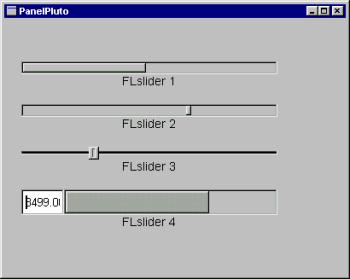
\includegraphics[scale=1]{flpanel} 


 FLpanel.
\subsection*{Examples}


  Here is an example of the flpanel opcode. It uses the files \emph{flpanel.orc}
 and \emph{flpanel.sco}
. 


 \textbf{Example 1. Example of the flpanel opcode.}

\begin{lstlisting}
/* flpanel.orc */
; Creates an empty window panel
sr = 44100
kr = 441
ksmps = 100
nchnls = 1

; Panel height in pixels
ipanelheight = 900
; Panel width in pixels
ipanelwidth = 400
; Horizontal position of the panel on screen in pixels
ix = 50
; Vertical position of the panel on screen in pixels
iy = 50

FLpanel "A Window Panel", ipanelheight, ipanelwidth, ix, iy
; End of panel contents
FLpanelEnd

;Run the widget thread!
FLrun

instr 1
endin
/* flpanel.orc */
        
\end{lstlisting}
\begin{lstlisting}
/* flpanel.sco */
; 'Dummy' score event of 1 hour.
f 0 3600
e
/* flpanel.sco */
        
\end{lstlisting}
\subsection*{See Also}


 \emph{FLgroup}
, \emph{FLgroupEnd}
, \emph{FLpack}
, \emph{FLpackEnd}
, \emph{FLpanelEnd}
, \emph{FLscroll}
, \emph{FLscrollEnd}
, \emph{FLtabs}
, \emph{FLtabsEnd}

\subsection*{Credits}


 Author: Gabriel Maldonado


 New in version 4.22


 Example written by Iain McCurdy, edited by Kevin Conder.
%\hline 


\begin{comment}
\begin{tabular}{lcr}
Previous &Home &Next \\
FLpackEnd &Up &FLpanelEnd

\end{tabular}


\end{document}
\end{comment}

\newpage
\begin{comment}
\documentclass[10pt]{article}
\usepackage{fullpage, graphicx, url}
\setlength{\parskip}{1ex}
\setlength{\parindent}{0ex}
\title{FLpanelEnd}
\begin{document}


\begin{tabular}{ccc}
The Alternative Csound Reference Manual & & \\
Previous & &Next

\end{tabular}

%\hline 
\end{comment}
\section{FLpanelEnd}
FLpanelEnd�--� Marks the end of a group of FLTK widgets contained inside of a window (panel). \subsection*{Description}


  Marks the end of a group of FLTK widgets contained inside of a window (panel). 
\subsection*{Syntax}


 \textbf{FLpanelEnd}

\subsection*{Performance}


  Containers are useful to format the graphic appearance of the widgets. The most important container is \emph{FLpanel}
, that actually creates a window. It can be filled with other containers and/or valuators or other kinds of widgets. 


  There are no k-rate arguments in containers. 
\subsection*{See Also}


 \emph{FLgroup}
, \emph{FLgroupEnd}
, \emph{FLpack}
, \emph{FLpackEnd}
, \emph{FLpanel}
, \emph{FLscroll}
, \emph{FLscrollEnd}
, \emph{FLtabs}
, \emph{FLtabsEnd}

\subsection*{Credits}


 Author: Gabriel Maldonado


 New in version 4.22
%\hline 


\begin{comment}
\begin{tabular}{lcr}
Previous &Home &Next \\
FLpanel &Up &FLprintk

\end{tabular}


\end{document}
\end{comment}

\newpage
\begin{comment}
\documentclass[10pt]{article}
\usepackage{fullpage, graphicx, url}
\setlength{\parskip}{1ex}
\setlength{\parindent}{0ex}
\title{FLprintk}
\begin{document}


\begin{tabular}{ccc}
The Alternative Csound Reference Manual & & \\
Previous & &Next

\end{tabular}

%\hline 
\end{comment}
\section{FLprintk}
FLprintk�--� A FLTK opcode that prints a k-rate value at specified intervals. \subsection*{Description}


 \emph{FLprintk}
 is similar to \emph{printk}
 but shows values of a k-rate signal in a text field instead of on the console. 
\subsection*{Syntax}


 \textbf{FLprintk}
 itime, kval, idisp
\subsection*{Initialization}


 \emph{itime}
 -- how much time in seconds is to elapse between updated displays. 


 \emph{idisp}
 -- a handle value that was output from a previous instance of the \emph{FLvalue}
 opcode to display the current value of the current valuator in the \emph{FLvalue}
 widget itself. If the user doesn't want to use this feature that displays current values, it must be set to a negative number by the user. 
\subsection*{Performance}


 \emph{kval}
 -- k-rate signal to be displayed. 


 \emph{FLprintk}
 is similar to \emph{printk}
, but shows values of a k-rate signal in a text field instead of showing it in the console. The \emph{idisp}
 argument must be filled with the \emph{ihandle}
 return value of a previous \emph{FLvalue}
 opcode. While \emph{FLvalue}
 should be placed in the header section of an orchestra inside an \emph{FLpanel}
/\emph{FLpanelEnd}
 block, \emph{FLprintk}
 must be placed inside an instrument to operate correctly. For this reason, it slows down performance and should be used for debugging purposes only. 
\subsection*{See Also}


 \emph{FLbox}
, \emph{FLbutBank}
, \emph{FLbutton}
, \emph{FLprintk2}
, \emph{FLvalue}

\subsection*{Credits}


 Author: Gabriel Maldonado


 New in version 4.22
%\hline 


\begin{comment}
\begin{tabular}{lcr}
Previous &Home &Next \\
FLpanelEnd &Up &FLprintk2

\end{tabular}


\end{document}
\end{comment}

\newpage
\begin{comment}
\documentclass[10pt]{article}
\usepackage{fullpage, graphicx, url}
\setlength{\parskip}{1ex}
\setlength{\parindent}{0ex}
\title{FLprintk2}
\begin{document}


\begin{tabular}{ccc}
The Alternative Csound Reference Manual & & \\
Previous & &Next

\end{tabular}

%\hline 
\end{comment}
\section{FLprintk2}
FLprintk2�--� A FLTK opcode that prints a new value every time a control-rate variable changes. \subsection*{Description}


 \emph{FLprintk2}
 is similar to \emph{FLprintk}
 but shows a k-rate variable's value only when it changes. 
\subsection*{Syntax}


 \textbf{FLprintk2}
 kval, idisp
\subsection*{Initialization}


 \emph{idisp}
 -- a handle value that was output from a previous instance of the \emph{FLvalue}
 opcode to display the current value of the current valuator in the \emph{FLvalue}
 widget itself. If the user doesn't want to use this feature that displays current values, it must be set to a negative number by the user. 
\subsection*{Performance}


 \emph{kval}
 -- k-rate signal to be displayed. 


 \emph{FLprintk2}
 is similar to \emph{FLprintk}
, but shows the k-rate variable's value only each time it changes. Useful for monitoring MIDI control changes when using sliders. It should be used for debugging purposes only, since it slows-down performance. 
\subsection*{See Also}


 \emph{FLbox}
, \emph{FLbutBank}
, \emph{FLbutton}
, \emph{FLprintk}
, \emph{FLvalue}

\subsection*{Credits}


 Author: Gabriel Maldonado


 New in version 4.22
%\hline 


\begin{comment}
\begin{tabular}{lcr}
Previous &Home &Next \\
FLprintk &Up &FLroller

\end{tabular}


\end{document}
\end{comment}

\newpage
\begin{comment}
\documentclass[10pt]{article}
\usepackage{fullpage, graphicx, url}
\setlength{\parskip}{1ex}
\setlength{\parindent}{0ex}
\title{FLroller}
\begin{document}


\begin{tabular}{ccc}
The Alternative Csound Reference Manual & & \\
Previous & &Next

\end{tabular}

%\hline 
\end{comment}
\section{FLroller}
FLroller�--� A FLTK widget that creates a transversal knob. \subsection*{Description}


 \emph{FLroller}
 is a sort of knob, but put transversally. 
\subsection*{Syntax}


 kout, ihandle \textbf{FLroller}
 ``label'', imin, imax, istep, iexp, itype, idisp, iwidth, iheight, ix, iy
\subsection*{Initialization}


 \emph{ihandle}
 -- a handle value (an integer number) that unequivocally references a corresponding widget. This is used by other opcodes that modify a widget's properties (see \emph{Modifying FLTK Widget Appearance}
). It is automatically output by \emph{FLroller}
 and must not be set by the user label. (The user label is a double-quoted string containing some user-provided text placed near the widget.) 


 \emph{``label''}
 -- a double-quoted string containing some user-provided text, placed near the corresponding widget. 


 \emph{imin}
 -- minimum value of output range. 


 \emph{imax}
 -- maximum value of output range. 


 \emph{istep}
 -- a floating-point number indicating the increment of valuator value corresponding to of each mouse click. The \emph{istep}
 argument allows the user to arbitrarily slow roller's motion, enabling arbitrary precision. 


 \emph{iexp}
 -- an integer number denoting the behaviour of valuator: 


 
\begin{itemize}
\item 

 0 = valuator output is linear

\item 

 -1 = valuator output is exponential


\end{itemize}


  All other positive numbers for \emph{iexp}
 indicate the number of an existing table that is used for indexing. Linear interpolation is provided in table indexing. A negative table number suppresses interpolation. 


 


\begin{tabular}{cc}
Warning &\textbf{IMPORTANT!}
 \\
� &

  Notice that the tables used by valuators must be created with the \emph{ftgen}
 opcode and placed in the orchestra before the corresponding valuator. They can not placed in the score. In fact, tables placed in the score are created later than the initialization of the opcodes placed in the header section of the orchestra. 


\end{tabular}



 \emph{itype}
 -- an integer number denoting the appearance of the valuator. 


  The \emph{itype}
 argument can be set to the following values: 


 
\begin{itemize}
\item 

 1 - horizontal roller

\item 

 2 - vertical roller


\end{itemize}


 \emph{idisp}
 -- a handle value that was output from a previous instance of the \emph{FLvalue}
 opcode to display the current value of the current valuator in the \emph{FLvalue}
 widget itself. If the user doesn't want to use this feature that displays current values, it must be set to a negative number by the user. 


 \emph{iwidth}
 -- width of widget. 


 \emph{iheight}
 -- height of widget. 


 \emph{ix}
 -- horizontal position of upper left corner of the valuator, relative to the upper left corner of corresponding window (expressed in pixels). 


 \emph{iy}
 -- vertical position of upper left corner of the valuator, relative to the upper left corner of corresponding window (expressed in pixels). 
\subsection*{Performance}


 \emph{kout}
 -- output value 


 \emph{FLroller}
 is a sort of knob, but put transversally: 


 
\includegraphics[scale=1]{flroller} 


 FLroller.
\subsection*{Examples}


  Here is an example of the flroller opcode. It uses the files \emph{flroller.orc}
 and \emph{flroller.sco}
. 


 \textbf{Example 1. Example of the flroller opcode.}

\begin{lstlisting}
/* flroller.orc */
; A sine with oscillator with flroller controlled frequency
sr = 44100
kr = 441
ksmps = 100
nchnls = 1

FLpanel "Frequency Roller", 900, 400, 50, 50
    ; Minimum value output by the roller
    imin = 200
    ; Maximum value output by the roller
    imax = 5000
    ; Increment with each pixel
    istep = 1
    ; Logarithmic type roller selected
    iexp = -1 
    ; Roller graphic type (1=horizontal)
    itype = 1
    ; Display handle (-1=not used)
    idisp = -1
    ; Width of the roller in pixels
    iwidth = 300
    ; Height of the roller in pixels
    iheight = 50 
    ; Distance of the left edge of the knob
    ; from the left edge of the panel 
    ix = 300
    ; Distance of the top edge of the knob
    ; from the top edge of the panel
    iy = 50

    gkfreq, ihandle FLroller "Frequency", imin, imax, istep, iexp, itype, idisp, iwidth, iheight, ix, iy
; End of panel contents
FLpanelEnd
; Run the widget thread!
FLrun

instr 1
    iamp = 15000
    ifn = 1
    asig oscili iamp, gkfreq, ifn
    out asig
endin
/* flroller.orc */
        
\end{lstlisting}
\begin{lstlisting}
/* flroller.sco */
; Function table that defines a single cycle
; of a sine wave.
f 1 0 1024 10 1

; Instrument 1 will play a note for 1 hour.
i 1 0 3600
e
/* flroller.sco */
        
\end{lstlisting}
\subsection*{See Also}


 \emph{FLcount}
, \emph{FLjoy}
, \emph{FLkeyb}
, \emph{FLknob}
, \emph{FLslider}
, \emph{FLtext}

\subsection*{Credits}


 Author: Gabriel Maldonado


 New in version 4.22


 Example written by Iain McCurdy, edited by Kevin Conder.
%\hline 


\begin{comment}
\begin{tabular}{lcr}
Previous &Home &Next \\
FLprintk2 &Up &FLrun

\end{tabular}


\end{document}
\end{comment}

\newpage
\begin{comment}
\documentclass[10pt]{article}
\usepackage{fullpage, graphicx, url}
\setlength{\parskip}{1ex}
\setlength{\parindent}{0ex}
\title{FLrun}
\begin{document}


\begin{tabular}{ccc}
The Alternative Csound Reference Manual & & \\
Previous & &Next

\end{tabular}

%\hline 
\end{comment}
\section{FLrun}
FLrun�--� Starts the FLTK widget thread. \subsection*{Description}


  Starts the FLTK widget thread. 
\subsection*{Syntax}


 \textbf{FLrun}

\subsection*{Performance}


  This opcode must be located at the end of all widget declarations. It has no arguments, and its purpose is to start the thread related to widgets. Widgets would not operate if \emph{FLrun}
 is missing. 
\subsection*{See Also}


 \emph{FLgetsnap}
, \emph{FLloadsnap}
, \emph{FLsavesnap}
, \emph{FLsetsnap}
, \emph{FLupdate}

\subsection*{Credits}


 Author: Gabriel Maldonado


 New in version 4.22
%\hline 


\begin{comment}
\begin{tabular}{lcr}
Previous &Home &Next \\
FLroller &Up &FLsavesnap

\end{tabular}


\end{document}
\end{comment}

\newpage
\begin{comment}
\documentclass[10pt]{article}
\usepackage{fullpage, graphicx, url}
\setlength{\parskip}{1ex}
\setlength{\parindent}{0ex}
\title{FLsavesnap}
\begin{document}


\begin{tabular}{ccc}
The Alternative Csound Reference Manual & & \\
Previous & &Next

\end{tabular}

%\hline 
\end{comment}
\section{FLsavesnap}
FLsavesnap�--� Saves all snapshots currently created into a file. \subsection*{Description}


 \emph{FLsavesnap}
 saves all snapshots currently created (i.e. the entire memory bank) into a file. 
\subsection*{Syntax}


 \textbf{FLsavesnap}
 ``filename''
\subsection*{Initialization}


 \emph{``filename''}
 -- a double-quoted string corresponding to a file to store a bank of snapshots. 
\subsection*{Performance}


 \emph{FLsavesnap}
 saves all snapshots currently created (i.e. the entire memory bank) into a file whose name is \emph{filename}
. Since the file is a text file, snapshot values can also be edited manually by means of a text editor. The format of the data stored in the file is the following (at present time, this could be changed in next Csound version): 


 
\begin{lstlisting}
----------- 0 -----------
FLvalue 0 0 1 0 ""
FLvalue 0 0 1 0 ""
FLvalue 0 0 1 0 ""
FLslider 331.946 80 5000 -1 "frequency of the first oscillator"
FLslider 385.923 80 5000 -1 "frequency of the second oscillator"
FLslider 80 80 5000 -1 "frequency of the third oscillator"
FLcount 0 0 10 0 "this index must point to the location number where snapshot is stored"
FLbutton 0 0 1 0 "Store snapshot to current index"
FLbutton 0 0 1 0 "Save snapshot bank to disk"
FLbutton 0 0 1 0 "Load snapshot bank from disk"
FLbox 0 0 1 0 ""
----------- 1 -----------
FLvalue 0 0 1 0 ""
FLvalue 0 0 1 0 ""
FLvalue 0 0 1 0 ""
FLslider 819.72 80 5000 -1 "frequency of the first oscillator"
FLslider 385.923 80 5000 -1 "frequency of the second oscillator"
FLslider 80 80 5000 -1 "frequency of the third oscillator"
FLcount 1 0 10 0 "this index must point to the location number where snapshot is stored"
FLbutton 0 0 1 0 "Store snapshot to current index"
FLbutton 0 0 1 0 "Save snapshot bank to disk"
FLbutton 0 0 1 0 "Load snapshot bank from disk"
FLbox 0 0 1 0 ""
----------- 2 -----------
..... etc...
----------- 3 -----------
..... etc...
---------------------------
        
\end{lstlisting}


 


  As you can see, each snapshot contain several lines. Each snapshot is separated from previous and next snapshot by a line of this kind: 


 ``-----------�snapshot�Num�-----------''\\ 
 ������
 Then there are several lines containing data. Each of these lines corresponds to a widget. 

  The first field of each line is an unquoted string containing opcode name corresponding to that widget. Second field is a number that expresses current value of a snapshot. In current version, this is the only field that can be modified manually. The third and fourth fields shows minimum and maximum values allowed for that valuator. The fifth field is a special number that indicates if the valuator is linear (value 0), exponential (value -1), or is indexed by a table interpolating values (negative table numbers) or non-interpolating (positive table numbers). The last field is a quoted string with the label of the widget. Last line of the file is always 


 ``---------------------------''\\ 
 ����
. \subsection*{See Also}


 \emph{FLgetsnap}
, \emph{FLloadsnap}
, \emph{FLrun}
, \emph{FLsetsnap}
, \emph{FLupdate}

\subsection*{Credits}


 Author: Gabriel Maldonado


 New in version 4.22
%\hline 


\begin{comment}
\begin{tabular}{lcr}
Previous &Home &Next \\
FLrun &Up &FLscroll

\end{tabular}


\end{document}
\end{comment}

\newpage
\begin{comment}
\documentclass[10pt]{article}
\usepackage{fullpage, graphicx, url}
\setlength{\parskip}{1ex}
\setlength{\parindent}{0ex}
\title{FLscroll}
\begin{document}


\begin{tabular}{ccc}
The Alternative Csound Reference Manual & & \\
Previous & &Next

\end{tabular}

%\hline 
\end{comment}
\section{FLscroll}
FLscroll�--� A FLTK opcode that adds scroll bars to an area. \subsection*{Description}


 \emph{FLscroll}
 adds scroll bars to an area. 
\subsection*{Syntax}


 \textbf{FLscroll}
 iwidth, iheight [, ix] [, iy]
\subsection*{Initialization}


 \emph{iwidth}
 -- width of widget. 


 \emph{iheight}
 -- height of widget. 


 \emph{ix}
 (optional) -- horizontal position of upper left corner of the valuator, relative to the upper left corner of corresponding window (expressed in pixels). 


 \emph{iy}
 (optional) -- vertical position of upper left corner of the valuator, relative to the upper left corner of corresponding window (expressed in pixels). 
\subsection*{Performance}


  Containers are useful to format the graphic appearance of the widgets. The most important container is \emph{FLpanel}
, that actually creates a window. It can be filled with other containers and/or valuators or other kinds of widgets. 


  There are no k-rate arguments in containers. 


 \emph{FLscroll}
 adds scroll bars to an area. Normally you must set arguments \emph{iwidth}
 and \emph{iheight}
 equal to that of the parent window or other parent container. \emph{ix}
 and \emph{iy}
 are optional since they normally are set to zero. For example the following code: 


 
\begin{lstlisting}
        FLpanel   "PanelPluto",400,300,100,100
        FLscroll  400,300
gk1,ih1 FLslider  "FLslider 1", 500, 1000, 2 ,1, -1, 300,15, 20,50
gk2,ih2 FLslider  "FLslider 2", 300, 5000, 2 ,3, -1, 300,15, 20,100
gk3,ih3 FLslider  "FLslider 3", 350, 1000, 2 ,5, -1, 300,15, 20,150
gk4,ih4 FLslider  "FLslider 4", 250, 5000, 1 ,11,-1, 300,30, 20,200
        FLscrollEnd
        FLpanelEnd
        
\end{lstlisting}


 
 will show scroll bars, when the main window size is reduced: 

 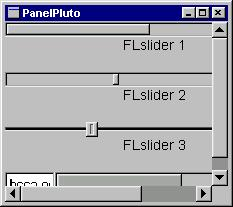
\includegraphics[scale=1]{flscroll} 


 FLscroll.
\subsection*{Examples}


  Here is an example of the flscroll opcode. It uses the files \emph{flscroll.orc}
 and \emph{flscroll.sco}
. 


 \textbf{Example 1. Example of the flscroll opcode.}

\begin{lstlisting}
/* flscroll.orc */
; Demonstration of the flscroll opcode which enables
; the use of widget sizes and placings beyond the
; dimensions of the containing panel
sr = 44100
kr = 441
ksmps = 100
nchnls = 1

FLpanel "Text Box", 420, 200, 50, 50
    iwidth = 420
    iheight = 200
    ix = 0
    iy = 0
    FLscroll iwidth, iheight, ix, iy
    ih3 FLbox "DRAG THE SCROLL BAR TO THE RIGHT IN ORDER TO READ THE REST OF THIS TEXT!", 1, 10, 20, 870, 30, 10, 100
    FLscrollEnd 
; End of panel contents
FLpanelEnd
; Run the widget thread!
FLrun

instr 1
endin
/* flscroll.orc */
        
\end{lstlisting}
\begin{lstlisting}
/* flscroll.sco */
; 'Dummy' score event of 1 hour.
f 0 3600
e
/* flscroll.sco */
        
\end{lstlisting}
\subsection*{See Also}


 \emph{FLgroup}
, \emph{FLgroupEnd}
, \emph{FLpack}
, \emph{FLpackEnd}
, \emph{FLpanel}
, \emph{FLpanelEnd}
, \emph{FLscrollEnd}
, \emph{FLtabs}
, \emph{FLtabsEnd}

\subsection*{Credits}


 Author: Gabriel Maldonado


 New in version 4.22


 Example written by Iain McCurdy, edited by Kevin Conder.
%\hline 


\begin{comment}
\begin{tabular}{lcr}
Previous &Home &Next \\
FLsavesnap &Up &FLscrollEnd

\end{tabular}


\end{document}
\end{comment}

\newpage
\begin{comment}
\documentclass[10pt]{article}
\usepackage{fullpage, graphicx, url}
\setlength{\parskip}{1ex}
\setlength{\parindent}{0ex}
\title{FLscrollEnd}
\begin{document}


\begin{tabular}{ccc}
The Alternative Csound Reference Manual & & \\
Previous & &Next

\end{tabular}

%\hline 
\end{comment}
\section{FLscrollEnd}
FLscrollEnd�--� A FLTK opcode that marks the end of an area with scrollbars. \subsection*{Description}


  A FLTK opcode that marks the end of an area with scrollbars. 
\subsection*{Syntax}


 \textbf{FLscrollEnd}

\subsection*{Performance}


  Containers are useful to format the graphic appearance of the widgets. The most important container is \emph{FLpanel}
, that actually creates a window. It can be filled with other containers and/or valuators or other kinds of widgets. 


  There are no k-rate arguments in containers. 
\subsection*{See Also}


 \emph{FLgroup}
, \emph{FLgroupEnd}
, \emph{FLpack}
, \emph{FLpackEnd}
, \emph{FLpanel}
, \emph{FLpanelEnd}
, \emph{FLscroll}
, \emph{FLtabs}
, \emph{FLtabsEnd}

\subsection*{Credits}


 Author: Gabriel Maldonado


 New in version 4.22
%\hline 


\begin{comment}
\begin{tabular}{lcr}
Previous &Home &Next \\
FLscroll &Up &FLsetAlign

\end{tabular}


\end{document}
\end{comment}

\newpage
\begin{comment}
\documentclass[10pt]{article}
\usepackage{fullpage, graphicx, url}
\setlength{\parskip}{1ex}
\setlength{\parindent}{0ex}
\title{FLsetAlign}
\begin{document}


\begin{tabular}{ccc}
The Alternative Csound Reference Manual & & \\
Previous & &Next

\end{tabular}

%\hline 
\end{comment}
\section{FLsetAlign}
FLsetAlign�--� Sets the text alignment of a label of a FLTK widget. \subsection*{Description}


 \emph{FLsetAlign}
 sets the text alignment of the label of the target widget. 
\subsection*{Syntax}


 \textbf{FLsetAlign}
 ialign, ihandle
\subsection*{Initialization}


 \emph{ialign}
 -- sets the alignment of the label text of widgets. 


  The legal values for the \emph{ialign}
 argument are: 


 
\begin{itemize}
\item 

 1 - align center

\item 

 2 - align top

\item 

 3 - align bottom

\item 

 4 - align left

\item 

 5 - align right

\item 

 6 - align top-left

\item 

 7 - align top-right

\item 

 8 - align bottom-left

\item 

 9 - align bottom-right


\end{itemize}


 \emph{ihandle}
 -- an integer number (used as unique identifier) taken from the output of a previously located widget opcode (which corresponds to the target widget). It is used to unequivocally identify the widget when modifying its appearance with this class of opcodes. The user must not set the \emph{ihandle}
 value directly, otherwise a Csound crash will occur. 
\subsection*{See Also}


 \emph{FLcolor}
, \emph{FLcolor2}
, \emph{FLhide}
, \emph{FLlabel}
, \emph{FLsetBox}
, \emph{FLsetColor}
, \emph{FLsetColor2}
, \emph{FLsetFont}
, \emph{FLsetPosition}
, \emph{FLsetSize}
, \emph{FLsetText}
, \emph{FLsetTextColor}
, \emph{FLsetTextSize}
, \emph{FLsetTextType}
, \emph{FLsetVal\_i}
, \emph{FLsetVal}
, \emph{FLshow}

\subsection*{Credits}


 Author: Gabriel Maldonado


 New in version 4.22
%\hline 


\begin{comment}
\begin{tabular}{lcr}
Previous &Home &Next \\
FLscrollEnd &Up &FLsetBox

\end{tabular}


\end{document}
\end{comment}

\newpage
\begin{comment}
\documentclass[10pt]{article}
\usepackage{fullpage, graphicx, url}
\setlength{\parskip}{1ex}
\setlength{\parindent}{0ex}
\title{FLsetBox}
\begin{document}


\begin{tabular}{ccc}
The Alternative Csound Reference Manual & & \\
Previous & &Next

\end{tabular}

%\hline 
\end{comment}
\section{FLsetBox}
FLsetBox�--� Sets the appearance of a box surrounding a FLTK widget. \subsection*{Description}


 \emph{FLsetBox}
 sets the appearance of a box surrounding the target widget. 
\subsection*{Syntax}


 \textbf{FLsetBox}
 itype, ihandle
\subsection*{Initialization}


 \emph{itype}
 -- an integer number that modify the appearance of the target widget. 


  Legal values for the \emph{itype}
 argument are: 


 
\begin{itemize}
\item 

 1 - flat box

\item 

 2 - up box

\item 

 3 - down box

\item 

 4 - thin up box

\item 

 5 - thin down box

\item 

 6 - engraved box

\item 

 7 - embossed box

\item 

 8 - border box

\item 

 9 - shadow box

\item 

 10 - rounded box

\item 

 11 - rounded box with shadow

\item 

 12 - rounded flat box

\item 

 13 - rounded up box

\item 

 14 - rounded down box

\item 

 15 - diamond up box

\item 

 16 - diamond down box

\item 

 17 - oval box

\item 

 18 - oval shadow box

\item 

 19 - oval flat box


\end{itemize}


 \emph{ihandle}
 -- an integer number (used as unique identifier) taken from the output of a previously located widget opcode (which corresponds to the target widget). It is used to unequivocally identify the widget when modifying its appearance with this class of opcodes. The user must not set the \emph{ihandle}
 value directly, otherwise a Csound crash will occur. 
\subsection*{See Also}


 \emph{FLcolor}
, \emph{FLcolor2}
, \emph{FLhide}
, \emph{FLlabel}
, \emph{FLsetAlign}
, \emph{FLsetColor}
, \emph{FLsetColor2}
, \emph{FLsetFont}
, \emph{FLsetPosition}
, \emph{FLsetSize}
, \emph{FLsetText}
, \emph{FLsetTextColor}
, \emph{FLsetTextSize}
, \emph{FLsetTextType}
, \emph{FLsetVal\_i}
, \emph{FLsetVal}
, \emph{FLshow}

\subsection*{Credits}


 Author: Gabriel Maldonado


 New in version 4.22
%\hline 


\begin{comment}
\begin{tabular}{lcr}
Previous &Home &Next \\
FLsetAlign &Up &FLsetColor

\end{tabular}


\end{document}
\end{comment}

\newpage
\begin{comment}
\documentclass[10pt]{article}
\usepackage{fullpage, graphicx, url}
\setlength{\parskip}{1ex}
\setlength{\parindent}{0ex}
\title{FLsetColor}
\begin{document}


\begin{tabular}{ccc}
The Alternative Csound Reference Manual & & \\
Previous & &Next

\end{tabular}

%\hline 
\end{comment}
\section{FLsetColor}
FLsetColor�--� Sets the primary color of a FLTK widget. \subsection*{Description}


 \emph{FLsetColor}
 sets the primary color of the target widget. 
\subsection*{Syntax}


 \textbf{FLsetColor}
 ired, igreen, iblue, ihandle
\subsection*{Initialization}


 \emph{ired}
 -- The red color of the target widget. The range for each RGB component is 0-255 


 \emph{igreen}
 -- The green color of the target widget. The range for each RGB component is 0-255 


 \emph{iblue}
 -- The blue color of the target widget. The range for each RGB component is 0-255 


 \emph{ihandle}
 -- an integer number (used as unique identifier) taken from the output of a previously located widget opcode (which corresponds to the target widget). It is used to unequivocally identify the widget when modifying its appearance with this class of opcodes. The user must not set the \emph{ihandle}
 value directly, otherwise a Csound crash will occur. 
\subsection*{Examples}


  Here is an example of the flsetcolor opcode. It uses the files \emph{flsetcolor.orc}
 and \emph{flsetcolor.sco}
. 


 \textbf{Example 1. Example of the flsetcolor opcode.}

\begin{lstlisting}
/* flsetcolor.orc */
; Using the opcode flsetcolor to change from the
; default colours for widgets
sr = 44100
kr = 441
ksmps = 100
nchnls = 1

FLpanel "Coloured Sliders", 900, 360, 50, 50
    gkfreq, ihandle FLslider "A Red Slider", 200, 5000, -1, 5, -1, 750, 30, 85, 50
    ired1 = 255
    igreen1 = 0
    iblue1 = 0
    FLsetColor ired1, igreen1, iblue1, ihandle

    gkfreq, ihandle FLslider "A Green Slider", 200, 5000, -1, 5, -1, 750, 30, 85, 150
    ired1 = 0
    igreen1 = 255
    iblue1 = 0
    FLsetColor ired1, igreen1, iblue1, ihandle

    gkfreq, ihandle FLslider "A Blue Slider", 200, 5000, -1, 5, -1, 750, 30, 85, 250
    ired1 = 0
    igreen1 = 0
    iblue1 = 255
    FLsetColor ired1, igreen1, iblue1, ihandle
; End of panel contents
FLpanelEnd
; Run the widget thread!
FLrun

instr 1
endin
/* flsetcolor.orc */
        
\end{lstlisting}
\begin{lstlisting}
/* flsetcolor.sco */
; 'Dummy' score event for 1 hour.
f 0 3600
e
/* flsetcolor.sco */
        
\end{lstlisting}
\subsection*{See Also}


 \emph{FLcolor}
, \emph{FLcolor2}
, \emph{FLhide}
, \emph{FLlabel}
, \emph{FLsetAlign}
, \emph{FLsetBox}
, \emph{FLsetColor2}
, \emph{FLsetFont}
, \emph{FLsetPosition}
, \emph{FLsetSize}
, \emph{FLsetText}
, \emph{FLsetTextColor}
, \emph{FLsetTextSize}
, \emph{FLsetTextType}
, \emph{FLsetVal\_i}
, \emph{FLsetVal}
, \emph{FLshow}

\subsection*{Credits}


 Author: Gabriel Maldonado


 New in version 4.22


 Example written by Iain McCurdy, edited by Kevin Conder.
%\hline 


\begin{comment}
\begin{tabular}{lcr}
Previous &Home &Next \\
FLsetBox &Up &FLsetColor2

\end{tabular}


\end{document}
\end{comment}

\newpage
\begin{comment}
\documentclass[10pt]{article}
\usepackage{fullpage, graphicx, url}
\setlength{\parskip}{1ex}
\setlength{\parindent}{0ex}
\title{FLsetColor2}
\begin{document}


\begin{tabular}{ccc}
The Alternative Csound Reference Manual & & \\
Previous & &Next

\end{tabular}

%\hline 
\end{comment}
\section{FLsetColor2}
FLsetColor2�--� Sets the secondary (or selection) color of a FLTK widget. \subsection*{Description}


 \emph{FLsetColor2}
 sets the secondary (or selection) color of the target widget. 
\subsection*{Syntax}


 \textbf{FLsetColor2}
 ired, igreen, iblue, ihandle
\subsection*{Initialization}


 \emph{ired}
 -- The red color of the target widget. The range for each RGB component is 0-255 


 \emph{igreen}
 -- The green color of the target widget. The range for each RGB component is 0-255 


 \emph{iblue}
 -- The blue color of the target widget. The range for each RGB component is 0-255 


 \emph{ihandle}
 -- an integer number (used as unique identifier) taken from the output of a previously located widget opcode (which corresponds to the target widget). It is used to unequivocally identify the widget when modifying its appearance with this class of opcodes. The user must not set the \emph{ihandle}
 value directly, otherwise a Csound crash will occur. 
\subsection*{See Also}


 \emph{FLcolor}
, \emph{FLcolor2}
, \emph{FLhide}
, \emph{FLlabel}
, \emph{FLsetAlign}
, \emph{FLsetBox}
, \emph{FLsetColor}
, \emph{FLsetFont}
, \emph{FLsetPosition}
, \emph{FLsetSize}
, \emph{FLsetText}
, \emph{FLsetTextColor}
, \emph{FLsetTextSize}
, \emph{FLsetTextType}
, \emph{FLsetVal\_i}
, \emph{FLsetVal}
, \emph{FLshow}

\subsection*{Credits}


 Author: Gabriel Maldonado


 New in version 4.22
%\hline 


\begin{comment}
\begin{tabular}{lcr}
Previous &Home &Next \\
FLsetColor &Up &FLsetFont

\end{tabular}


\end{document}
\end{comment}

\newpage
\begin{comment}
\documentclass[10pt]{article}
\usepackage{fullpage, graphicx, url}
\setlength{\parskip}{1ex}
\setlength{\parindent}{0ex}
\title{FLsetFont}
\begin{document}


\begin{tabular}{ccc}
The Alternative Csound Reference Manual & & \\
Previous & &Next

\end{tabular}

%\hline 
\end{comment}
\section{FLsetFont}
FLsetFont�--� Sets the font type of a FLTK widget. \subsection*{Description}


 \emph{FLsetFont}
 sets the font type of the target widget. 
\subsection*{Syntax}


 \textbf{FLsetFont}
 ifont, ihandle
\subsection*{Initialization}


 \emph{ifont}
 -- sets the the font type of the label of a widget. 


  Legal values for ifont argument are: 


 
\begin{itemize}
\item 

 1 - Helvetica (same as Arial under Windows)

\item 

 2 - Helvetica Bold

\item 

 3 - Helvetica Italic

\item 

 4 - Helvetica Bold Italic

\item 

 5 - Courier

\item 

 6 - Courier Bold

\item 

 7 - Courier Italic

\item 

 8 - Courier Bold Italic

\item 

 9 - Times

\item 

 10 - Times Bold

\item 

 11 - Times Italic

\item 

 12 - Times Bold Italic

\item 

 13 - Symbol

\item 

 14 - Screen

\item 

 15 - Screen Bold

\item 

 16 - Dingbats


\end{itemize}


 \emph{ihandle}
 -- an integer number (used as unique identifier) taken from the output of a previously located widget opcode (which corresponds to the target widget). It is used to unequivocally identify the widget when modifying its appearance with this class of opcodes. The user must not set the \emph{ihandle}
 value directly, otherwise a Csound crash will occur. 
\subsection*{See Also}


 \emph{FLcolor}
, \emph{FLcolor2}
, \emph{FLhide}
, \emph{FLlabel}
, \emph{FLsetAlign}
, \emph{FLsetBox}
, \emph{FLsetColor}
, \emph{FLsetColor2}
, \emph{FLsetPosition}
, \emph{FLsetSize}
, \emph{FLsetText}
, \emph{FLsetTextColor}
, \emph{FLsetTextSize}
, \emph{FLsetTextType}
, \emph{FLsetVal\_i}
, \emph{FLsetVal}
, \emph{FLshow}

\subsection*{Credits}


 Author: Gabriel Maldonado


 New in version 4.22
%\hline 


\begin{comment}
\begin{tabular}{lcr}
Previous &Home &Next \\
FLsetColor2 &Up &FLsetPosition

\end{tabular}


\end{document}
\end{comment}

\newpage
\begin{comment}
\documentclass[10pt]{article}
\usepackage{fullpage, graphicx, url}
\setlength{\parskip}{1ex}
\setlength{\parindent}{0ex}
\title{FLsetPosition}
\begin{document}


\begin{tabular}{ccc}
The Alternative Csound Reference Manual & & \\
Previous & &Next

\end{tabular}

%\hline 
\end{comment}
\section{FLsetPosition}
FLsetPosition�--� Sets the position of a FLTK widget. \subsection*{Description}


 \emph{FLsetPosition}
 sets the position of the target widget according to the \emph{ix}
 and \emph{iy}
 arguments. 
\subsection*{Syntax}


 \textbf{FLsetPosition}
 ix, iy, ihandle
\subsection*{Initialization}


 \emph{ix}
 -- horizontal position of upper left corner of the valuator, relative to the upper left corner of corresponding window (expressed in pixels). 


 \emph{iy}
 -- vertical position of upper left corner of the valuator, relative to the upper left corner of corresponding window (expressed in pixels). 


 \emph{ihandle}
 -- an integer number (used as unique identifier) taken from the output of a previously located widget opcode (which corresponds to the target widget). It is used to unequivocally identify the widget when modifying its appearance with this class of opcodes. The user must not set the \emph{ihandle}
 value directly, otherwise a Csound crash will occur. 
\subsection*{See Also}


 \emph{FLcolor}
, \emph{FLcolor2}
, \emph{FLhide}
, \emph{FLlabel}
, \emph{FLsetAlign}
, \emph{FLsetBox}
, \emph{FLsetColor}
, \emph{FLsetColor2}
, \emph{FLsetFont}
, \emph{FLsetSize}
, \emph{FLsetText}
, \emph{FLsetTextColor}
, \emph{FLsetTextSize}
, \emph{FLsetTextType}
, \emph{FLsetVal\_i}
, \emph{FLsetVal}
, \emph{FLshow}

\subsection*{Credits}


 Author: Gabriel Maldonado


 New in version 4.22
%\hline 


\begin{comment}
\begin{tabular}{lcr}
Previous &Home &Next \\
FLsetFont &Up &FLsetSize

\end{tabular}


\end{document}
\end{comment}

\newpage
\begin{comment}
\documentclass[10pt]{article}
\usepackage{fullpage, graphicx, url}
\setlength{\parskip}{1ex}
\setlength{\parindent}{0ex}
\title{FLsetSize}
\begin{document}


\begin{tabular}{ccc}
The Alternative Csound Reference Manual & & \\
Previous & &Next

\end{tabular}

%\hline 
\end{comment}
\section{FLsetSize}
FLsetSize�--� Resizes a FLTK widget. \subsection*{Description}


 \emph{FLsetSize}
 resizes the target widget (not the size of its text) according to the \emph{iwidth}
 and \emph{iheight}
 arguments. 
\subsection*{Syntax}


 \textbf{FLsetSize}
 iwidth, iheight, ihandle
\subsection*{Initialization}


 \emph{iwidth}
 -- width of widget. 


 \emph{iheight}
 -- height of widget. 


 \emph{ihandle}
 -- an integer number (used as unique identifier) taken from the output of a previously located widget opcode (which corresponds to the target widget). It is used to unequivocally identify the widget when modifying its appearance with this class of opcodes. The user must not set the \emph{ihandle}
 value directly, otherwise a Csound crash will occur. 
\subsection*{See Also}


 \emph{FLcolor}
, \emph{FLcolor2}
, \emph{FLhide}
, \emph{FLlabel}
, \emph{FLsetAlign}
, \emph{FLsetBox}
, \emph{FLsetColor}
, \emph{FLsetColor2}
, \emph{FLsetFont}
, \emph{FLsetPosition}
, \emph{FLsetText}
, \emph{FLsetTextColor}
, \emph{FLsetTextSize}
, \emph{FLsetTextType}
, \emph{FLsetVal\_i}
, \emph{FLsetVal}
, \emph{FLshow}

\subsection*{Credits}


 Author: Gabriel Maldonado


 New in version 4.22
%\hline 


\begin{comment}
\begin{tabular}{lcr}
Previous &Home &Next \\
FLsetPosition &Up &FLsetsnap

\end{tabular}


\end{document}
\end{comment}

\newpage
\begin{comment}
\documentclass[10pt]{article}
\usepackage{fullpage, graphicx, url}
\setlength{\parskip}{1ex}
\setlength{\parindent}{0ex}
\title{FLsetsnap}
\begin{document}


\begin{tabular}{ccc}
The Alternative Csound Reference Manual & & \\
Previous & &Next

\end{tabular}

%\hline 
\end{comment}
\section{FLsetsnap}
FLsetsnap�--� Stores the current status of all FLTK valuators into a snapshot location. \subsection*{Description}


 \emph{FLsetsnap}
 stores the current status of all valuators present in the orchestra into a snapshot location (in memory). 
\subsection*{Syntax}


 inumsnap, inumval \textbf{FLsetsnap}
 index [, ifn]
\subsection*{Initialization}


 \emph{inumsnap}
 -- current number of snapshots. 


 \emph{inumval}
 -- number of valuators (whose value is stored in a snapshot) present in current orchestra. 


 \emph{index}
 -- a number referring unequivocally to a snapshot. Several snapshots can be stored in the same bank. 


 \emph{ifn}
 (optional) -- optional argument referring to an already allocated table, to store values of a snapshot. 
\subsection*{Performance}


  The \emph{FLsetsnap}
 opcode stores current status of all valuators present in the orchestra into a snapshot location (in memory). Any number of snapshots can be stored in the current bank. Banks are structures that only exist in memory, there are no other reference to them other that they can be accessed by \emph{FLsetsnap}
, \emph{FLsavesnap}
, \emph{FLloadsnap}
 and \emph{FLgetsnap}
 opcodes. Only a single bank can be present in memory. 


  If the optional \emph{ifn}
 argument refers to an already allocated and valid table, the snapshot will be stored in the table instead of in the bank. So that table can be accessed from other Csound opcodes. 


  The \emph{index}
 argument unequivocally refers to a determinate snapshot. If the value of \emph{index}
 refers to a previously stored snapshot, all its old values will be replaced with current ones. If \emph{index}
 refers to a snapshot that doesn't exist, a new snapshot will be created. If the \emph{index}
 value is not adjacent with that of a previously created snapshot, some empty snapshots will be created. For example, if a location with \emph{index}
 0 contains the only and unique snapshot present in a bank and the user stores a new snapshot using \emph{index}
 5, all locations between 1 and 4 will automatically contain empty snapshots. Empty snapshots don't contain any data and are neutral. 


 \emph{FLsetsnap}
 outputs the current number of snapshots (the \emph{inumsnap}
 argument) and the total number of values stored in each snapshot (\emph{inumval}
). \emph{inumval}
 is equal to the number of valuators present in the orchestra. 
\subsection*{See Also}


 \emph{FLgetsnap}
, \emph{FLloadsnap}
, \emph{FLrun}
, \emph{FLsavesnap}
, \emph{FLupdate}

\subsection*{Credits}


 Author: Gabriel Maldonado


 New in version 4.22
%\hline 


\begin{comment}
\begin{tabular}{lcr}
Previous &Home &Next \\
FLsetSize &Up &FLsetText

\end{tabular}


\end{document}
\end{comment}

\newpage
\begin{comment}
\documentclass[10pt]{article}
\usepackage{fullpage, graphicx, url}
\setlength{\parskip}{1ex}
\setlength{\parindent}{0ex}
\title{FLsetText}
\begin{document}


\begin{tabular}{ccc}
The Alternative Csound Reference Manual & & \\
Previous & &Next

\end{tabular}

%\hline 
\end{comment}
\section{FLsetText}
FLsetText�--� Sets the label of a FLTK widget. \subsection*{Description}


 \emph{FLsetText}
 sets the label of the target widget to the double-quoted text string provided with the \emph{itext}
 argument. 
\subsection*{Syntax}


 \textbf{FLsetText}
 ``itext'', ihandle
\subsection*{Initialization}


 \emph{``itext''}
 -- a double-quoted string denoting the text of the label of the widget. 


 \emph{ihandle}
 -- an integer number (used as unique identifier) taken from the output of a previously located widget opcode (which corresponds to the target widget). It is used to unequivocally identify the widget when modifying its appearance with this class of opcodes. The user must not set the \emph{ihandle}
 value directly, otherwise a Csound crash will occur. 
\subsection*{See Also}


 \emph{FLcolor}
, \emph{FLcolor2}
, \emph{FLhide}
, \emph{FLlabel}
, \emph{FLsetAlign}
, \emph{FLsetBox}
, \emph{FLsetColor}
, \emph{FLsetColor2}
, \emph{FLsetFont}
, \emph{FLsetPosition}
, \emph{FLsetSize}
, \emph{FLsetTextColor}
, \emph{FLsetTextSize}
, \emph{FLsetTextType}
, \emph{FLsetVal\_i}
, \emph{FLsetVal}
, \emph{FLshow}

\subsection*{Credits}


 Author: Gabriel Maldonado


 New in version 4.22
%\hline 


\begin{comment}
\begin{tabular}{lcr}
Previous &Home &Next \\
FLsetsnap &Up &FLsetTextColor

\end{tabular}


\end{document}
\end{comment}

\newpage
\begin{comment}
\documentclass[10pt]{article}
\usepackage{fullpage, graphicx, url}
\setlength{\parskip}{1ex}
\setlength{\parindent}{0ex}
\title{FLsetTextColor}
\begin{document}


\begin{tabular}{ccc}
The Alternative Csound Reference Manual & & \\
Previous & &Next

\end{tabular}

%\hline 
\end{comment}
\section{FLsetTextColor}
FLsetTextColor�--� Sets the color of the text label of a FLTK widget. \subsection*{Description}


 \emph{FLsetTextColor}
 sets the color of the text label of the target widget. 
\subsection*{Syntax}


 \textbf{FLsetTextColor}
 isize, ihandle
\subsection*{Initialization}


 \emph{isize}
 -- size of the font of the target widget. Normal values are in the order of 15. Greater numbers enlarge font size, while smaller numbers reduce it. 


 \emph{ihandle}
 -- an integer number (used as unique identifier) taken from the output of a previously located widget opcode (which corresponds to the target widget). It is used to unequivocally identify the widget when modifying its appearance with this class of opcodes. The user must not set the \emph{ihandle}
 value directly, otherwise a Csound crash will occur. 
\subsection*{See Also}


 \emph{FLcolor}
, \emph{FLcolor2}
, \emph{FLhide}
, \emph{FLlabel}
, \emph{FLsetAlign}
, \emph{FLsetBox}
, \emph{FLsetColor}
, \emph{FLsetColor2}
, \emph{FLsetFont}
, \emph{FLsetPosition}
, \emph{FLsetSize}
, \emph{FLsetText}
, \emph{FLsetTextSize}
, \emph{FLsetTextType}
, \emph{FLsetVal\_i}
, \emph{FLsetVal}
, \emph{FLshow}

\subsection*{Credits}


 Author: Gabriel Maldonado


 New in version 4.22
%\hline 


\begin{comment}
\begin{tabular}{lcr}
Previous &Home &Next \\
FLsetText &Up &FLsetTextSize

\end{tabular}


\end{document}
\end{comment}

\newpage
\begin{comment}
\documentclass[10pt]{article}
\usepackage{fullpage, graphicx, url}
\setlength{\parskip}{1ex}
\setlength{\parindent}{0ex}
\title{FLsetTextSize}
\begin{document}


\begin{tabular}{ccc}
The Alternative Csound Reference Manual & & \\
Previous & &Next

\end{tabular}

%\hline 
\end{comment}
\section{FLsetTextSize}
FLsetTextSize�--� Sets the size of the text label of a FLTK widget. \subsection*{Description}


 \emph{FLsetTextSize}
 sets the size of the text label of the target widget. 
\subsection*{Syntax}


 \textbf{FLsetTextSize}
 isize, ihandle
\subsection*{Initialization}


 \emph{isize}
 -- size of the font of the target widget. Normal values are in the order of 15. Greater numbers enlarge font size, while smaller numbers reduce it. 


 \emph{ihandle}
 -- an integer number (used as unique identifier) taken from the output of a previously located widget opcode (which corresponds to the target widget). It is used to unequivocally identify the widget when modifying its appearance with this class of opcodes. The user must not set the \emph{ihandle}
 value directly, otherwise a Csound crash will occur. 
\subsection*{See Also}


 \emph{FLcolor}
, \emph{FLcolor2}
, \emph{FLhide}
, \emph{FLlabel}
, \emph{FLsetAlign}
, \emph{FLsetBox}
, \emph{FLsetColor}
, \emph{FLsetColor2}
, \emph{FLsetFont}
, \emph{FLsetPosition}
, \emph{FLsetSize}
, \emph{FLsetText}
, \emph{FLsetTextColor}
, \emph{FLsetTextType}
, \emph{FLsetVal\_i}
, \emph{FLsetVal}
, \emph{FLshow}

\subsection*{Credits}


 Author: Gabriel Maldonado


 New in version 4.22
%\hline 


\begin{comment}
\begin{tabular}{lcr}
Previous &Home &Next \\
FLsetTextColor &Up &FLsetTextType

\end{tabular}


\end{document}
\end{comment}

\newpage
\begin{comment}
\documentclass[10pt]{article}
\usepackage{fullpage, graphicx, url}
\setlength{\parskip}{1ex}
\setlength{\parindent}{0ex}
\title{FLsetTextType}
\begin{document}


\begin{tabular}{ccc}
The Alternative Csound Reference Manual & & \\
Previous & &Next

\end{tabular}

%\hline 
\end{comment}
\section{FLsetTextType}
FLsetTextType�--� Sets some font attributes of the text label of a FLTK widget. \subsection*{Description}


 \emph{FLsetTextType}
 sets some attributes related to the fonts of the text label of the target widget. 
\subsection*{Syntax}


 \textbf{FLsetTextType}
 itype, ihandle
\subsection*{Initialization}


 \emph{itype}
 -- an integer number that modify the appearance of the target widget. 


  The legal values of \emph{itype}
 are: 


 
\begin{itemize}
\item 

 0 - normal label

\item 

 1 - no label (hides the text)

\item 

 2 - symbol label (see below)

\item 

 3 - shadow label

\item 

 4 - engraved label

\item 

 5- embossed label

\item 

 6- bitmap label (not implemented yet)

\item 

 7- pixmap label (not implemented yet)

\item 

 8- image label (not implemented yet)

\item 

 9- multi label (not implemented yet)

\item 

 10- free-type label (not implemented yet)


\end{itemize}
 When using \emph{itype}
=3 (symbol label), it is possible to assign a graphical symbol instead of the text label of the target widget. In this case, the string of the target label must always start with ``@''. If it starts with something else (or the symbol is not found), the label is drawn normally. The following symbols are supported: 

 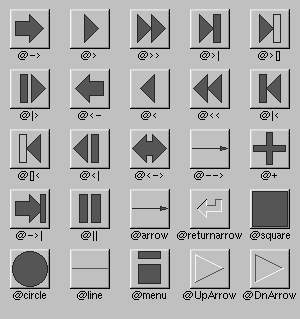
\includegraphics[scale=1]{symbols} 


 FLTK label supported symbols.


  The @ sign may be followed by the following optional ``formatting'' characters, in this order: 


 
\begin{enumerate}
\item 

 ``\#'' forces square scaling rather than distortion to the widget's shape.

\item 

 +[1-9] or -[1-9] tweaks the scaling a little bigger or smaller.

\item 

 [1-9] rotates by a multiple of 45 degrees. ``6'' does nothing, the others point in the direction of that key on a numeric keypad.


\end{enumerate}


  Notice that with \emph{FLbox}
 and \emph{FLbutton}
, it is not necessary to call \emph{FLsetTextType}
 opcode at all in order to use a symbol. In this case, it is sufficient to set a label starting with ``@'' followed by the proper formatting string. 


 \emph{ihandle}
 -- an integer number (used as unique identifier) taken from the output of a previously located widget opcode (which corresponds to the target widget). It is used to unequivocally identify the widget when modifying its appearance with this class of opcodes. The user must not set the \emph{ihandle}
 value directly, otherwise a Csound crash will occur. 
\subsection*{See Also}


 \emph{FLcolor}
, \emph{FLcolor2}
, \emph{FLhide}
, \emph{FLlabel}
, \emph{FLsetAlign}
, \emph{FLsetBox}
, \emph{FLsetColor}
, \emph{FLsetColor2}
, \emph{FLsetFont}
, \emph{FLsetPosition}
, \emph{FLsetSize}
, \emph{FLsetText}
, \emph{FLsetTextColor}
, \emph{FLsetTextSize}
, \emph{FLsetVal\_i}
, \emph{FLsetVal}
, \emph{FLshow}

\subsection*{Credits}


 Author: Gabriel Maldonado


 New in version 4.22
%\hline 


\begin{comment}
\begin{tabular}{lcr}
Previous &Home &Next \\
FLsetTextSize &Up &FLsetVal\_i

\end{tabular}


\end{document}
\end{comment}

\newpage
\begin{comment}
\documentclass[10pt]{article}
\usepackage{fullpage, graphicx, url}
\setlength{\parskip}{1ex}
\setlength{\parindent}{0ex}
\title{FLsetVal}
\begin{document}


\begin{tabular}{ccc}
The Alternative Csound Reference Manual & & \\
Previous & &Next

\end{tabular}

%\hline 
\end{comment}
\section{FLsetVal}
FLsetVal�--� Sets the value of a FLTK valuator at control-rate. \subsection*{Description}


 \emph{FLsetVal}
 is almost identical to \emph{FLsetVal\_i}
. Except it operates at k-rate and it affects the target valuator only when \emph{ktrig}
 is set to a non-zero value. 
\subsection*{Syntax}


 \textbf{FLsetVal}
 ktrig, kvalue, ihandle
\subsection*{Initialization}


 \emph{ihandle}
 -- an integer number (used as unique identifier) taken from the output of a previously located widget opcode (which corresponds to the target widget). It is used to unequivocally identify the widget when modifying its appearance with this class of opcodes. The user must not set the \emph{ihandle}
 value directly, otherwise a Csound crash will occur. 
\subsection*{Performance}


 \emph{ktrig}
 -- not implemented yet. 


 \emph{kvalue}
 -- not implemented yet. 
\subsection*{See Also}


 \emph{FLcolor}
, \emph{FLcolor2}
, \emph{FLhide}
, \emph{FLlabel}
, \emph{FLsetAlign}
, \emph{FLsetBox}
, \emph{FLsetColor}
, \emph{FLsetColor2}
, \emph{FLsetFont}
, \emph{FLsetPosition}
, \emph{FLsetSize}
, \emph{FLsetText}
, \emph{FLsetTextColor}
, \emph{FLsetTextSize}
, \emph{FLsetTextType}
, \emph{FLsetVal\_i}
, \emph{FLshow}

\subsection*{Credits}


 Author: Gabriel Maldonado


 New in version 4.22
%\hline 


\begin{comment}
\begin{tabular}{lcr}
Previous &Home &Next \\
FLsetVal\_i &Up &FLshow

\end{tabular}


\end{document}
\end{comment}

\newpage
\begin{comment}
\documentclass[10pt]{article}
\usepackage{fullpage, graphicx, url}
\setlength{\parskip}{1ex}
\setlength{\parindent}{0ex}
\title{FLsetVal\_i}
\begin{document}


\begin{tabular}{ccc}
The Alternative Csound Reference Manual & & \\
Previous & &Next

\end{tabular}

%\hline 
\end{comment}
\section{FLsetVal\_i}
FLsetVal\_i�--� Sets the value of a FLTK valuator to a number provided by the user. \subsection*{Description}


 \emph{FLsetVal\_i}
 forces the value of a valuator to a number provided by the user. 
\subsection*{Syntax}


 \textbf{FLsetVal\_i}
 kvalue, ihandle
\subsection*{Initialization}


 \emph{ihandle}
 -- an integer number (used as unique identifier) taken from the output of a previously located widget opcode (which corresponds to the target widget). It is used to unequivocally identify the widget when modifying its appearance with this class of opcodes. The user must not set the \emph{ihandle}
 value directly, otherwise a Csound crash will occur. 
\subsection*{Performance}


 \emph{kvalue}
 -- not implemented yet. 
\subsection*{See Also}


 \emph{FLcolor}
, \emph{FLcolor2}
, \emph{FLhide}
, \emph{FLlabel}
, \emph{FLsetAlign}
, \emph{FLsetBox}
, \emph{FLsetColor}
, \emph{FLsetColor2}
, \emph{FLsetFont}
, \emph{FLsetPosition}
, \emph{FLsetSize}
, \emph{FLsetText}
, \emph{FLsetTextColor}
, \emph{FLsetTextSize}
, \emph{FLsetTextType}
, \emph{FLsetVal}
, \emph{FLshow}

\subsection*{Credits}


 Author: Gabriel Maldonado


 New in version 4.22
%\hline 


\begin{comment}
\begin{tabular}{lcr}
Previous &Home &Next \\
FLsetTextType &Up &FLsetVal

\end{tabular}


\end{document}
\end{comment}

\newpage
\begin{comment}
\documentclass[10pt]{article}
\usepackage{fullpage, graphicx, url}
\setlength{\parskip}{1ex}
\setlength{\parindent}{0ex}
\title{FLshow}
\begin{document}


\begin{tabular}{ccc}
The Alternative Csound Reference Manual & & \\
Previous & &Next

\end{tabular}

%\hline 
\end{comment}
\section{FLshow}
FLshow�--� Restores the visibility of a previously hidden FLTK widget. \subsection*{Description}


 \emph{FLshow}
 restores the visibility of a previously hidden widget. 
\subsection*{Syntax}


 \textbf{FLshow}
 ihandle
\subsection*{Initialization}


 \emph{ihandle}
 -- an integer number (used as unique identifier) taken from the output of a previously located widget opcode (which corresponds to the target widget). It is used to unequivocally identify the widget when modifying its appearance with this class of opcodes. The user must not set the \emph{ihandle}
 value directly, otherwise a Csound crash will occur. 
\subsection*{See Also}


 \emph{FLcolor}
, \emph{FLcolor2}
, \emph{FLhide}
, \emph{FLlabel}
, \emph{FLsetAlign}
, \emph{FLsetBox}
, \emph{FLsetColor}
, \emph{FLsetColor2}
, \emph{FLsetFont}
, \emph{FLsetPosition}
, \emph{FLsetSize}
, \emph{FLsetText}
, \emph{FLsetTextColor}
, \emph{FLsetTextSize}
, \emph{FLsetTextType}
, \emph{FLsetVal\_i}
, \emph{FLsetVal}

\subsection*{Credits}


 Author: Gabriel Maldonado


 New in version 4.22
%\hline 


\begin{comment}
\begin{tabular}{lcr}
Previous &Home &Next \\
FLsetVal &Up &FLslidBnk

\end{tabular}


\end{document}
\end{comment}

\newpage
\begin{comment}
\documentclass[10pt]{article}
\usepackage{fullpage, graphicx, url}
\setlength{\parskip}{1ex}
\setlength{\parindent}{0ex}
\title{FLslidBnk}
\begin{document}


\begin{tabular}{ccc}
The Alternative Csound Reference Manual & & \\
Previous & &Next

\end{tabular}

%\hline 
\end{comment}
\section{FLslidBnk}
FLslidBnk�--� A FLTK widget containing a bank of horizontal sliders. \subsection*{Description}


 \emph{FLslidBnk}
 is a widget containing a bank of horizontal sliders. 
\subsection*{Syntax}


 \textbf{FLslidBnk}
 ``names'', inumsliders [, ioutable] [, iwidth] [, iheight] [, ix] [, iy] [, itypetable] [, iexptable] [, istart\_index] [, iminmaxtable]
\subsection*{Initialization}


 \emph{``names''}
 -- a double-quoted string containing the names of each slider. Each slider can have a different name. Separate each name with ``@'' character, for example: ``frequency@amplitude@cutoff''. It is possible to not provide any name by giving a single space `` ``. In this case, the opcode will automatically assign a progressive number as a label for each slider. 


 \emph{inumsliders}
 -- the number of sliders. 


 \emph{ioutable}
 (optional, default=0) -- number of a previously-allocated table in which to store output values of each slider. The user must be sure that table size is large enough to contain all output cells, otherwise a segfault will crash Csound. By assigning zero to this argument, the output will be directed to the zak space in the k-rate zone. In this case, the zak space must be previously allocated with the \emph{zakinit}
 opcode and the user must be sure that the allocation size is big enough to cover all sliders. The default value is zero (i.e. store output in zak space). 


 \emph{istart\_index}
 (optional, default=0) -- an integer number referring to a starting offset of output cell locations. It can be positive to allow multiple banks of sliders to output in the same table or in the zak space. The default value is zero (no offset). 


 \emph{iminmaxtable}
 (optional, default=0) -- number of a previously-defined table containing a list of min-max pairs, referred to each slider. A zero value defaults to the 0 to 1 range for all sliders without necessity to provide a table. The default value is zero. 


 \emph{iexptable}
 (optional, default=0) -- number of a previously-defined table containing a list of identifiers (i.e. integer numbers) provided to modify the behaviour of each slider independently. Identifiers can assume the following values: 


 
\begin{itemize}
\item 

 -1 -- exponential curve response

\item 

 0 -- linear response

\item 

 number $>$ than 0 -- follow the curve of a previously-defined table to shape the response of the corresponding slider. In this case, the number corresponds to table number.


\end{itemize}
 You can assume that all sliders of the bank have the same response curve (exponential or linear). In this case, you can assign -1 or 0 to \emph{iexptable}
 without worrying about previously defining any table. The default value is zero (all sliders have a linear response, without having to provide a table). 

 \emph{itypetable}
 (optional, default=0) -- number of a previously-defined table containing a list of identifiers (i.e. integer numbers) provided to modify the aspect of each individual slider independently. Identifiers can assume the following values: 


 
\begin{itemize}
\item 

 0 = Nice slider

\item 

 1 = Fill slider

\item 

 3 = Normal slider

\item 

 5 = Nice slider

\item 

 7 = Nice slider with down-box


\end{itemize}
 You can assume that all sliders of the bank have the same aspect. In this case, you can assign a negative number to \emph{itypetable}
 without worrying about previously defining any table. Negative numbers have the same meaning of the corresponding positive identifiers with the difference that the same aspect is assigned to all sliders. You can also assign a random aspect to each slider by setting \emph{itypetable}
 to a negative number lower than -7. The default value is zero (all sliders have the aspect of nice sliders, without having to provide a table). 

 \emph{iwidth}
 (optional) -- width of the rectangular area containing all sliders of the bank, excluding text labels, that are placed to the left of that area. 


 \emph{iheight}
 (optional) -- height of the rectangular area containing all sliders of the bank, excluding text labels, that are placed to the left of that area. 


 \emph{ix}
 (optional) -- horizontal position of the upper left corner of the rectangular area containing all sliders belonging to the bank. You have to leave enough space, at the left of that rectangle, in order to make sure labels of sliders to be visible. This is because the labels themselves are external to the rectangular area. 


 \emph{iy}
 (optional) -- vertical position of the upper left corner of the rectangular area containing all sliders belonging to the bank. You have to leave enough space, at the left of that rectangle, in order to make sure labels of sliders to be visible. This is because the labels themselves are external to the rectangular area. 
\subsection*{Performance}


  There are no k-rate arguments, even if cells of the output table (or the zak space) are updated at k-rate. 


 \emph{FLslidBnk}
 is a widget containing a bank of horizontal sliders. Any number of sliders can be placed into the bank (\emph{inumsliders}
 argument). The output of all sliders is stored into a previously allocated table or into the zak space (\emph{ioutable}
 argument). It is possible to determine the first location of the table (or of the zak space) in which to store the output of the first slider by means of \emph{istart\_index}
 argument. 


  Each slider can have an individual label that is placed to the left of it. Labels are defined by the \emph{``names''}
 argument. The output range of each slider can be individually set by means of an external table (\emph{iminmaxtable}
 argument). The curve response of each slider can be set individually, by means of a list of identifiers placed in a table (\emph{iexptable}
 argument). It is possible to define the aspect of each slider independently or to make all sliders have the same aspect (\emph{itypetable}
 argument). 


  The \emph{iwidth}
, \emph{iheight}
, \emph{ix}
, and \emph{iy}
 arguments determine width, height, horizontal and vertical position of the rectangular area containing sliders. Notice that the label of each slider is placed to the left of them and is not included in the rectangular area containing sliders. So the user should leave enough space to the left of the bank by assigning a proper \emph{ix}
 value in order to leave labels visible. 
\subsection*{See Also}


 \emph{FLslider}

\subsection*{Credits}


 Author: Gabriel Maldonado


 New in version 4.22
%\hline 


\begin{comment}
\begin{tabular}{lcr}
Previous &Home &Next \\
FLshow &Up &FLslider

\end{tabular}


\end{document}
\end{comment}

\newpage
\begin{comment}
\documentclass[10pt]{article}
\usepackage{fullpage, graphicx, url}
\setlength{\parskip}{1ex}
\setlength{\parindent}{0ex}
\title{FLslider}
\begin{document}


\begin{tabular}{ccc}
The Alternative Csound Reference Manual & & \\
Previous & &Next

\end{tabular}

%\hline 
\end{comment}
\section{FLslider}
FLslider�--� Puts a slider into the corresponding FLTK container. \subsection*{Description}


 \emph{FLslider}
 puts a slider into the corresponding container. 
\subsection*{Syntax}


 kout, ihandle \textbf{FLslider}
 ``label'', imin, imax, iexp, itype, idisp, iwidth, iheight, ix, iy
\subsection*{Initialization}


 \emph{ihandle}
 -- a handle value (an integer number) that unequivocally references a corresponding widget. This is used by other opcodes that modify a widget's properties (see \emph{Modifying FLTK Widget Appearance}
). It is automatically output by \emph{FLslider}
 and must not be set by the user label. (The user label is a double-quoted string containing some user-provided text placed near the widget.) 


 \emph{``label''}
 -- a double-quoted string containing some user-provided text, placed near the corresponding widget. 


 \emph{imin}
 -- minimum value of output range. 


 \emph{imax}
 -- maximum value of output range. 


  The \emph{imin}
 argument may be greater than \emph{imax}
 argument. This has the effect of ``reversing'' the object so the larger values are in the opposite direction. This also switches which end of the filled sliders is filled. 


 \emph{iexp}
 -- an integer number denoting the behaviour of valuator: 


 
\begin{itemize}
\item 

 0 = valuator output is linear

\item 

 -1 = valuator output is exponential


\end{itemize}


  All other positive numbers for \emph{iexp}
 indicate the number of an existing table that is used for indexing. Linear interpolation is provided in table indexing. A negative table number suppresses interpolation. 


 


\begin{tabular}{cc}
Warning &\textbf{IMPORTANT!}
 \\
� &

  Notice that the tables used by valuators must be created with the \emph{ftgen}
 opcode and placed in the orchestra before the corresponding valuator. They can not placed in the score. In fact, tables placed in the score are created later than the initialization of the opcodes placed in the header section of the orchestra. 


\end{tabular}



 \emph{itype}
 -- an integer number denoting the appearance of the valuator. 


  The \emph{itype}
 argument can be set to the following values: 


 
\begin{itemize}
\item 

 1 - shows a horizontal fill slider

\item 

 2 - a vertical fill slider

\item 

 3 - a horizontal engraved slider

\item 

 4 - a vertical engraved slider

\item 

 5 - a horizontal nice slider

\item 

 6 - a vertical nice slider

\item 

 7 - a horizontal up-box nice slider

\item 

 8 - a vertical up-box nice slider


\end{itemize}


 
\includegraphics[scale=1]{flslider_horizontal-fill} 


 FLslider - a horizontal fill slider (itype=1).


 
\includegraphics[scale=1]{flslider_horizontal-engraved} 


 FLslider - a horizontal engraved slider (itype=3).


 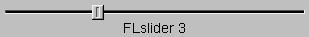
\includegraphics[scale=1]{flslider_horizontal-nice} 


 FLslider - a horizontal nice slider (itype=5).


 \emph{idisp}
 -- a handle value that was output from a previous instance of the \emph{FLvalue}
 opcode to display the current value of the current valuator in the \emph{FLvalue}
 widget itself. If the user doesn't want to use this feature that displays current values, it must be set to a negative number by the user. 


 \emph{iwidth}
 -- width of widget. 


 \emph{iheight}
 -- height of widget. 


 \emph{ix}
 -- horizontal position of upper left corner of the valuator, relative to the upper left corner of corresponding window (expressed in pixels). 


 \emph{iy}
 -- vertical position of upper left corner of the valuator, relative to the upper left corner of corresponding window (expressed in pixels). 
\subsection*{Performance}


 \emph{kout}
 -- output value 
\subsection*{Examples}


  Here is an example of the flslider opcode. It uses the files \emph{flslider.orc}
 and \emph{flslider.sco}
. 


 \textbf{Example 1. Example of the flslider opcode.}

\begin{lstlisting}
/* flslider.orc */
; A sine with oscillator with flslider controlled frequency
sr = 44100
kr = 441
ksmps = 100
nchnls = 1

FLpanel "Frequency Slider", 900, 400, 50, 50
    ; Minimum value output by the slider
    imin = 200
    ; Maximum value output by the slider
    imax = 5000
    ; Logarithmic type slider selected
    iexp = -1
    ; Slider graphic type (5='nice' slider)
    itype = 5 
    ; Display handle (-1=not used)
    idisp = -1
    ; Width of the slider in pixels
    iwidth = 750
    ; Height of the slider in pixels
    iheight = 30
    ; Distance of the left edge of the slider
    ; from the left edge of the panel
    ix = 125
    ; Distance of the top edge of the slider 
    ; from the top edge of the panel
    iy = 50

    gkfreq, ihandle FLslider "Frequency", imin, imax, iexp, itype, idisp, iwidth, iheight, ix, iy
; End of panel contents
FLpanelEnd
; Run the widget thread!
FLrun

instr 1
    iamp = 15000
    ifn = 1
    asig oscili iamp, gkfreq, ifn
    out asig
endin
/* flslider.orc */
        
\end{lstlisting}
\begin{lstlisting}
/* flslider.sco */
; Function table that defines a single cycle
; of a sine wave.
f 1 0 1024 10 1

; Instrument 1 will play a note for 1 hour.
i 1 0 3600
e
/* flslider.sco */
        
\end{lstlisting}
\subsection*{See Also}


 \emph{FLcount}
, \emph{FLjoy}
, \emph{FLkeyb}
, \emph{FLknob}
, \emph{FLroller}
, \emph{FLslidBnk}
, \emph{FLtext}

\subsection*{Credits}


 Author: Gabriel Maldonado


 New in version 4.22


 February 2004. Thanks to a note from Dave Phillips, deleted the extraneous istep parameter.


 Example written by Iain McCurdy, edited by Kevin Conder.
%\hline 


\begin{comment}
\begin{tabular}{lcr}
Previous &Home &Next \\
FLslidBnk &Up &FLtabs

\end{tabular}


\end{document}
\end{comment}

\newpage
\begin{comment}
\documentclass[10pt]{article}
\usepackage{fullpage, graphicx, url}
\setlength{\parskip}{1ex}
\setlength{\parindent}{0ex}
\title{FLtabs}
\begin{document}


\begin{tabular}{ccc}
The Alternative Csound Reference Manual & & \\
Previous & &Next

\end{tabular}

%\hline 
\end{comment}
\section{FLtabs}
FLtabs�--� Creates a tabbed FLTK interface. \subsection*{Description}


 \emph{FLtabs}
 is the ``file card tabs'' interface that allows useful to display several areas containing widgets in the same windows, alternatively. It must be used together with \emph{FLgroup}
, another container that groups child widgets. 
\subsection*{Syntax}


 \textbf{FLtabs}
 iwidth, iheight, ix, iy
\subsection*{Initialization}


 \emph{iwidth}
 -- width of widget. 


 \emph{iheight}
 -- height of widget. 


 \emph{ix}
 -- horizontal position of upper left corner of the valuator, relative to the upper left corner of corresponding window. Expressed in pixels. 


 \emph{iy}
 -- vertical position of upper left corner of the valuator, relative to the upper left corner of corresponding window. Expressed in pixels. 
\subsection*{Performance}


  Containers are useful to format the graphic appearance of the widgets. The most important container is \emph{FLpanel}
, that actually creates a window. It can be filled with other containers and/or valuators or other kinds of widgets. 


  There are no k-rate arguments in containers. 


 \emph{FLtabs}
 is a ``file card tabs'' interface that is useful to display several alternate areas containing widgets in the same window. 


 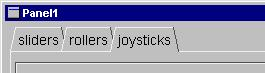
\includegraphics[scale=1]{fltabs} 


 FLtabs.


  It must be used together with \emph{FLgroup}
, another FLTK container opcode that groups child widgets. 
\subsection*{Examples}


  The following example code: 


 
\begin{lstlisting}
        FLpanel "Panel1",450,550,100,100
        FLscroll  450,550,0,0
        FLtabs  400,550, 5,5
        FLgroup "sliders",380,500, 10,40,1
gk1,ihs FLslider  "FLslider 1", 500, 1000, 2 ,1, -1, 300,15, 20,50
gk2,ihs FLslider  "FLslider 2", 300, 5000, 2 ,3, -1, 300,15, 20,100
gk3,ihs FLslider  "FLslider 3", 350, 1000, 2 ,5, -1, 300,15, 20,150
gk4,ihs FLslider  "FLslider 4", 250, 5000, 1 ,11, -1, 300,30, 20,200
gk5,ihs FLslider  "FLslider 5", 220, 8000, 2 ,1, -1, 300,15, 20,250
gk6,ihs FLslider  "FLslider 6", 1, 5000, 1 ,13, -1, 300,15, 20,300
gk7,ihs FLslider  "FLslider 7", 870, 5000, 1 ,15, -1, 300,30, 20,350
gk8,ihs FLslider  "FLslider 8", 20, 20000, 2 ,6, -1, 30,400, 350,50
        FLgroupEnd

        FLgroup "rollers",380,500, 10,30,2
gk1,ihr FLroller  "FLroller 1", 50, 1000,.1,2 ,1 ,-1, 200,22, 20,50
gk2,ihr FLroller  "FLroller 2", 80, 5000,1,2 ,1 ,-1, 200,22, 20,100
gk3,ihr FLroller  "FLroller 3", 50, 1000,.1,2 ,1 ,-1, 200,22, 20,150
gk4,ihr FLroller  "FLroller 4", 80, 5000,1,2 ,1 ,-1, 200,22, 20,200
gk5,ihr FLroller  "FLroller 5", 50, 1000,.1,2 ,1 ,-1, 200,22, 20,250
gk6,ihr FLroller  "FLroller 6", 80, 5000,1,2 ,1 ,-1, 200,22, 20,300
gk7,ihr FLroller  "FLroller 7",50, 5000,1,1 ,2 ,-1, 30,300, 280,50
        FLgroupEnd

        FLgroup "joysticks",380,500, 10,40,3
gk1,gk2,ihj1,ihj2 FLjoy "FLjoy", 50, 18000, 50, 18000,2,2,-1,-1,300,300,30,60
        FLgroupEnd

        FLtabsEnd
        FLscrollEnd
        FLpanelEnd
        
\end{lstlisting}


 
 ...will produce the following result: 

 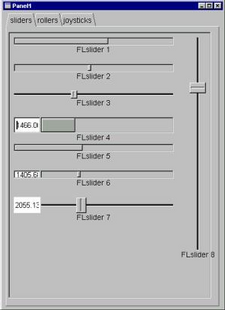
\includegraphics[scale=1]{fltabs_sliders-tab} 


 FLtabs example, sliders tab.


 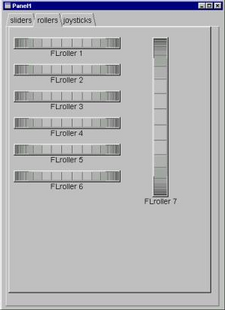
\includegraphics[scale=1]{fltabs_rollers-tab} 


 FLtabs example, rollers tab.


 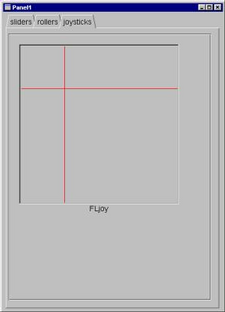
\includegraphics[scale=1]{fltabs_joysticks-tab} 


 FLtabs example, joysticks tab.
 (Each picture shows a different tab selection inside the same window.) \subsection*{Examples}


  Here is an example of the fltabs opcode. It uses the files \emph{fltabs.orc}
 and \emph{fltabs.sco}
. 


 \textbf{Example 1. Example of the fltabs opcode.}

\begin{lstlisting}
/* fltabs.orc */
; A single oscillator with frequency, amplitude and
; panning controls on separate file tab cards
sr = 44100
kr = 441
ksmps = 100
nchnls = 2

FLpanel "Tabs", 300, 350, 100, 100
itabswidth = 280
itabsheight = 330
ix = 5
iy = 5
FLtabs itabswidth,itabsheight, ix,iy

    itab1width = 280
    itab1height = 300
    itab1x = 10
    itab1y = 40
    FLgroup "Tab 1", itab1width, itab1height, itab1x, itab1y
        gkfreq, i1 FLknob "Frequency", 200, 5000, -1, 1, -1, 70, 70, 130
        FLsetVal_i 400, i1
    FLgroupEnd

    itab2width = 280
    itab2height = 300
    itab2x = 10
    itab2y = 40
    FLgroup "Tab 2", itab2width, itab2height, itab2x, itab2y
        gkamp, i2 FLknob "Amplitude", 0, 15000, 0, 1, -1, 70, 70, 130
        FLsetVal_i 15000, i2
    FLgroupEnd

    itab3width = 280
    itab3height = 300
    itab3x = 10
    itab3y = 40
    FLgroup "Tab 3", itab3width, itab3height, itab3x, itab3y
        gkpan, i3 FLknob "Pan position", 0, 1, 0, 1, -1, 70, 70, 130
        FLsetVal_i 0.5, i3
    FLgroupEnd
FLtabsEnd
FLpanelEnd
; Run the widget thread!
FLrun

instr 1
    ifn = 1
    asig oscili gkamp, gkfreq, ifn
    outs asig*(1-gkpan), asig*gkpan
endin
/* fltabs.orc */
        
\end{lstlisting}
\begin{lstlisting}
/* fltabs.sco */
; Function table that defines a single cycle
; of a sine wave.
f 1 0 1024 10 1

; Instrument 1 will play a note for 1 hour.
i 1 0 3600
e
/* fltabs.sco */
        
\end{lstlisting}
\subsection*{See Also}


 \emph{FLgroup}
, \emph{FLgroupEnd}
, \emph{FLpack}
, \emph{FLpackEnd}
, \emph{FLpanel}
, \emph{FLpanelEnd}
, \emph{FLscroll}
, \emph{FLscrollEnd}
, \emph{FLtabsEnd}

\subsection*{Credits}


 Author: Gabriel Maldonado


 New in version 4.22


 Example written by Iain McCurdy, edited by Kevin Conder.
%\hline 


\begin{comment}
\begin{tabular}{lcr}
Previous &Home &Next \\
FLslider &Up &FLtabsEnd

\end{tabular}


\end{document}
\end{comment}

\newpage
\begin{comment}
\documentclass[10pt]{article}
\usepackage{fullpage, graphicx, url}
\setlength{\parskip}{1ex}
\setlength{\parindent}{0ex}
\title{FLtabsEnd}
\begin{document}


\begin{tabular}{ccc}
The Alternative Csound Reference Manual & & \\
Previous & &Next

\end{tabular}

%\hline 
\end{comment}
\section{FLtabsEnd}
FLtabsEnd�--� Marks the end of a tabbed FLTK interface. \subsection*{Description}


  Marks the end of a tabbed FLTK interface. 
\subsection*{Syntax}


 \textbf{FLtabsEnd}

\subsection*{Performance}


  Containers are useful to format the graphic appearance of the widgets. The most important container is \emph{FLpanel}
, that actually creates a window. It can be filled with other containers and/or valuators or other kinds of widgets. 


  There are no k-rate arguments in containers. 
\subsection*{See Also}


 \emph{FLgroup}
, \emph{FLgroupEnd}
, \emph{FLpack}
, \emph{FLpackEnd}
, \emph{FLpanel}
, \emph{FLpanelEnd}
, \emph{FLscroll}
, \emph{FLscrollEnd}
, \emph{FLtabs}

\subsection*{Credits}


 Author: Gabriel Maldonado


 New in version 4.22
%\hline 


\begin{comment}
\begin{tabular}{lcr}
Previous &Home &Next \\
FLtabs &Up &FLtext

\end{tabular}


\end{document}
\end{comment}

\newpage
\begin{comment}
\documentclass[10pt]{article}
\usepackage{fullpage, graphicx, url}
\setlength{\parskip}{1ex}
\setlength{\parindent}{0ex}
\title{FLtext}
\begin{document}


\begin{tabular}{ccc}
The Alternative Csound Reference Manual & & \\
Previous & &Next

\end{tabular}

%\hline 
\end{comment}
\section{FLtext}
FLtext�--� A FLTK widget opcode that creates a textbox. \subsection*{Description}


 \emph{\emph{FLtext}
 allows the user to modify a parameter value by directly typing it into a text field.}

\subsection*{Syntax}


 kout, ihandle \textbf{FLtext}
 ``label'', imin, imax, istep, itype, iwidth, iheight, ix, iy
\subsection*{Initialization}


 \emph{ihandle}
 -- a handle value (an integer number) that unequivocally references a corresponding widget. This is used by other opcodes that modify a widget's properties (see \emph{Modifying FLTK Widget Appearance}
). It is automatically output by \emph{FLtext}
 and must not be set by the user label. (The user label is a double-quoted string containing some user-provided text placed near the widget.) 


 \emph{``label''}
 -- a double-quoted string containing some user-provided text, placed near corresponding widget. 


 \emph{imin}
 -- minimum value of output range. 


 \emph{imax}
 -- maximum value of output range. 


 \emph{istep}
 -- a floating-point number indicating the increment of valuator value corresponding to of each mouse click. The \emph{istep}
 argument allows the user to arbitrarily slow roller's motion, enabling arbitrary precision. 


 \emph{itype}
 -- an integer number denoting the appearance of the valuator. 


  The \emph{itype}
 argument can be set to the following values: 


 
\begin{itemize}
\item 

 1 - normal behaviour

\item 

 2 - dragging operation is suppressed, instead it will appear two arrow buttons. A mouse-click on one of these buttons can increase/decrease the output value.

\item 

 3 - text editing is suppressed, only mouse dragging modifies the output value.


\end{itemize}


 \emph{iwidth}
 -- width of widget. 


 \emph{iheight}
 -- height of widget. 


 \emph{ix}
 -- horizontal position of upper left corner of the valuator, relative to the upper left corner of corresponding window (expressed in pixels). 


 \emph{iy}
 -- vertical position of upper left corner of the valuator, relative to the upper left corner of corresponding window (expressed in pixels). 
\subsection*{Performance}


 \emph{kout}
 -- output value 


 \emph{FLtext}
 allows the user to modify a parameter value by directly typing it into a text field: 


 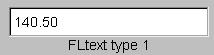
\includegraphics[scale=1]{fltext} 


 FLtext.
 Its value can also be modified by clicking on it and dragging the mouse horizontally. The \emph{istep}
 argument allows the user to arbitrarily set the response on mouse dragging. \subsection*{Examples}


  Here is an example of the fltext opcode. It uses the files \emph{fltext.orc}
 and \emph{fltext.sco}
. 


 \textbf{Example 1. Example of the fltext opcode.}

\begin{lstlisting}
/* fltext.orc */
; A sine with oscillator with fltext box controlled
; frequency either click and drag or double click and
; type to change frequency value
sr = 44100
kr = 441
ksmps = 100
nchnls = 1

FLpanel "Frequency Text Box", 270, 600, 50, 50
    ; Minimum value output by the text box
    imin = 200
    ; Maximum value output by the text box
    imax = 5000
    ; Step size
    istep = 1
    ; Text box graphic type
    itype = 1
    ; Width of the text box in pixels
    iwidth = 70
    ; Height of the text box in pixels
    iheight = 30
    ; Distance of the left edge of the text box 
    ; from the left edge of the panel
    ix = 100
    ; Distance of the top edge of the text box
    ; from the top edge of the panel
    iy = 300

    gkfreq,ihandle FLtext "Enter the frequency", imin, imax, istep, itype, iwidth, iheight, ix, iy
; End of panel contents
FLpanelEnd
; Run the widget thread!
FLrun

instr 1
    iamp = 15000
    ifn = 1
    asig oscili iamp, gkfreq, ifn
    out asig
endin
/* fltext.orc */
        
\end{lstlisting}
\begin{lstlisting}
/* fltext.sco */
; Function table that defines a single cycle
; of a sine wave.
f 1 0 1024 10 1

; Instrument 1 will play a note for 1 hour.
i 1 0 3600
e
/* fltext.sco */
        
\end{lstlisting}
\subsection*{See Also}


 \emph{FLcount}
, \emph{FLjoy}
, \emph{FLkeyb}
, \emph{FLknob}
, \emph{FLroller}
, \emph{FLslider}

\subsection*{Credits}


 Author: Gabriel Maldonado


 New in version 4.22


 Example written by Iain McCurdy, edited by Kevin Conder.
%\hline 


\begin{comment}
\begin{tabular}{lcr}
Previous &Home &Next \\
FLtabsEnd &Up &FLupdate

\end{tabular}


\end{document}
\end{comment}

\newpage
\begin{comment}
\documentclass[10pt]{article}
\usepackage{fullpage, graphicx, url}
\setlength{\parskip}{1ex}
\setlength{\parindent}{0ex}
\title{FLupdate}
\begin{document}


\begin{tabular}{ccc}
The Alternative Csound Reference Manual & & \\
Previous & &Next

\end{tabular}

%\hline 
\end{comment}
\section{FLupdate}
FLupdate�--� Same as the FLrun opcode. \subsection*{Description}


  Same as the \emph{FLrun}
 opcode. 
\subsection*{Syntax}


 \textbf{FLupdate}

%\hline 


\begin{comment}
\begin{tabular}{lcr}
Previous &Home &Next \\
FLtext &Up &FLvalue

\end{tabular}


\end{document}
\end{comment}

\newpage
\begin{comment}
\documentclass[10pt]{article}
\usepackage{fullpage, graphicx, url}
\setlength{\parskip}{1ex}
\setlength{\parindent}{0ex}
\title{FLvalue}
\begin{document}


\begin{tabular}{ccc}
The Alternative Csound Reference Manual & & \\
Previous & &Next

\end{tabular}

%\hline 
\end{comment}
\section{FLvalue}
FLvalue�--� Shows the current value of a FLTK valuator. \subsection*{Description}


 \emph{FLvalue}
 shows current the value of a valuator in a text field. 
\subsection*{Syntax}


 ihandle \textbf{FLvalue}
 ``label'', iwidth, iheight, ix, iy
\subsection*{Initialization}


 \emph{ihandle}
 -- handle value (an integer number) that unequivocally references the corresponding valuator. It can be used for the \emph{idisp}
 argument of a valuator. 


 \emph{``label''}
 -- a double-quoted string containing some user-provided text, placed near the corresponding widget. 


 \emph{iwidth}
 -- width of widget. 


 \emph{iheight}
 -- height of widget. 


 \emph{ix}
 -- horizontal position of upper left corner of the valuator, relative to the upper left corner of corresponding window (expressed in pixels). 


 \emph{iy}
 -- vertical position of upper left corner of the valuator, relative to the upper left corner of corresponding window (expressed in pixels). 
\subsection*{Performance}


  Note that \emph{FLvalue}
 is not a valuator and its value is fixed. Its value cannot be modified. 


 \emph{FLvalue}
 shows the current values of a valuator in a text field. It outputs \emph{ihandle}
 that can then be used for the \emph{idisp}
 argument of a valuator (see the \emph{FLTK Valuators section}
). In this way, the values of that valuator will be dynamically be shown in a text field. 
\subsection*{Examples}


  Here is an example of the flvalue opcode. It uses the files \emph{flvalue.orc}
 and \emph{flvalue.sco}
. 


 \textbf{Example 1. Example of the flvalue opcode.}

\begin{lstlisting}
/* flvalue.orc */
; Using the opcode flvalue to display the output of a slider 
sr = 44100
kr = 441
ksmps = 100
nchnls = 1

FLpanel "Value Display Box", 900, 200, 50, 50
    ; Width of the value display box in pixels
    iwidth = 50
    ; Height of the value display box in pixels
    iheight = 20
    ; Distance of the left edge of the value display
    ; box from the left edge of the panel
    ix = 65
    ; Distance of the top edge of the value display
    ; box from the top edge of the panel
    iy = 55

    idisp FLvalue "Hertz", iwidth, iheight, ix, iy
    gkfreq, ihandle FLslider "Frequency", 200, 5000, -1, 5, idisp, 750, 30, 125, 50
    FLsetVal_i 500, ihandle
; End of panel contents
FLpanelEnd
; Run the widget thread!
FLrun

instr 1
    iamp = 15000
    ifn = 1
    asig oscili iamp, gkfreq, ifn
    out asig
endin
/* flvalue.orc */
        
\end{lstlisting}
\begin{lstlisting}
/* flvalue.sco */
; Function table that defines a single cycle
; of a sine wave.
f 1 0 1024 10 1

; Instrument 1 will play a note for 1 hour.
i 1 0 3600
e
/* flvalue.sco */
        
\end{lstlisting}
\subsection*{See Also}


 \emph{FLbox}
, \emph{FLbutBank}
, \emph{FLbutton}
, \emph{FLprintk}
, \emph{FLprintk2}

\subsection*{Credits}


 Author: Gabriel Maldonado


 New in version 4.22


 Example written by Iain McCurdy, edited by Kevin Conder.
%\hline 


\begin{comment}
\begin{tabular}{lcr}
Previous &Home &Next \\
FLupdate &Up &fmb3

\end{tabular}


\end{document}
\end{comment}

\newpage
\begin{comment}
\documentclass[10pt]{article}
\usepackage{fullpage, graphicx, url}
\setlength{\parskip}{1ex}
\setlength{\parindent}{0ex}
\title{fmb3}
\begin{document}


\begin{tabular}{ccc}
The Alternative Csound Reference Manual & & \\
Previous & &Next

\end{tabular}

%\hline 
\end{comment}
\section{fmb3}
fmb3�--� Uses FM synthesis to create a Hammond B3 organ sound. \subsection*{Description}


  Uses FM synthesis to create a Hammond B3 organ sound. It comes from a family of FM sounds, all using 4 basic oscillators and various architectures, as used in the TX81Z synthesizer. 
\subsection*{Syntax}


 ar \textbf{fmb3}
 kamp, kfreq, kc1, kc2, kvdepth, kvrate, ifn1, ifn2, ifn3, ifn4, ivfn
\subsection*{Initialization}


 \emph{fmb3}
 takes 5 tables for initialization. The first 4 are the basic inputs and the last is the low frequency oscillator (LFO) used for vibrato. The last table should usually be a sine wave. 


  The initial waves should be: 


 
\begin{itemize}
\item 

 \emph{ifn1}
 -- sine wave

\item 

 \emph{ifn2}
 -- sine wave

\item 

 \emph{ifn3}
 -- sine wave

\item 

 \emph{ifn4}
 -- sine wave


\end{itemize}
\subsection*{Performance}


 \emph{kamp}
 -- Amplitude of note. 


 \emph{kfreq}
 -- Frequency of note played. 


 \emph{kc1, kc2}
 -- Controls for the synthesizer: 


 
\begin{itemize}
\item 

 \emph{kc1}
 -- Total mod index

\item 

 \emph{kc2}
 -- Crossfade of two modulators

\item 

 \emph{Algorithm}
 -- 4


\end{itemize}


 \emph{kvdepth}
 -- Vibrator depth 


 \emph{kvrate}
 -- Vibrator rate 
\subsection*{Examples}


  Here is an example of the fmb3 opcode. It uses the files \emph{fmb3.orc}
 and \emph{fmb3.sco}
. 


 \textbf{Example 1. Example of the fmb3 opcode.}

\begin{lstlisting}
/* fmb3.orc */
; Initialize the global variables.
sr = 44100
kr = 4410
ksmps = 10
nchnls = 1

; Instrument #1.
instr 1
  kamp = 15000
  kfreq = 440
  kc1 = 5
  kc2 = 5
  kvdepth = 0.005
  kvrate = 6
  ifn1 = 1
  ifn2 = 1
  ifn3 = 1
  ifn4 = 1
  ivfn = 1

  a1 fmb3 kamp, kfreq, kc1, kc2, kvdepth, kvrate,  \
          ifn1, ifn2, ifn3, ifn4, ivfn
  out a1
endin
/* fmb3.orc */
        
\end{lstlisting}
\begin{lstlisting}
/* fmb3.sco */
; Table #1, a sine wave.
f 1 0 32768 10 1

; Play Instrument #1 for two seconds.
i 1 0 2
e
/* fmb3.sco */
        
\end{lstlisting}
\subsection*{See Also}


 \emph{fmbell}
, \emph{fmmetal}
, \emph{fmpercfl}
, \emph{fmrhode}
, \emph{fmwurlie}

\subsection*{Credits}


 


 


\begin{tabular}{ccc}
Author: John ffitch (after Perry Cook) &University of Bath, Codemist Ltd. &Bath, UK

\end{tabular}



 


 Example written by Kevin Conder.


 New in Csound version 3.47
%\hline 


\begin{comment}
\begin{tabular}{lcr}
Previous &Home &Next \\
FLvalue &Up &fmbell

\end{tabular}


\end{document}
\end{comment}

\newpage
\begin{comment}
\documentclass[10pt]{article}
\usepackage{fullpage, graphicx, url}
\setlength{\parskip}{1ex}
\setlength{\parindent}{0ex}
\title{fmbell}
\begin{document}


\begin{tabular}{ccc}
The Alternative Csound Reference Manual & & \\
Previous & &Next

\end{tabular}

%\hline 
\end{comment}
\section{fmbell}
fmbell�--� Uses FM synthesis to create a tublar bell sound. \subsection*{Description}


  Uses FM synthesis to create a tublar bell sound. It comes from a family of FM sounds, all using 4 basic oscillators and various architectures, as used in the TX81Z synthesizer. 
\subsection*{Syntax}


 ar \textbf{fmbell}
 kamp, kfreq, kc1, kc2, kvdepth, kvrate, ifn1, ifn2, ifn3, ifn4, ivfn
\subsection*{Initialization}


  All these opcodes take 5 tables for initialization. The first 4 are the basic inputs and the last is the low frequency oscillator (LFO) used for vibrato. The last table should usually be a sine wave. 


  The initial waves should be: 


 
\begin{itemize}
\item 

 \emph{ifn1}
 -- sine wave

\item 

 \emph{ifn2}
 -- sine wave

\item 

 \emph{ifn3}
 -- sine wave

\item 

 \emph{ifn4}
 -- sine wave


\end{itemize}
\subsection*{Performance}


 \emph{kamp}
 -- Amplitude of note. 


 \emph{kfreq}
 -- Frequency of note played. 


 \emph{kc1, kc2}
 -- Controls for the synthesizer: 


 
\begin{itemize}
\item 

 \emph{kc1}
 -- Mod index 1

\item 

 \emph{kc2}
 -- Crossfade of two outputs

\item 

 \emph{Algorithm}
 -- 5


\end{itemize}


 \emph{kvdepth}
 -- Vibrator depth 


 \emph{kvrate}
 -- Vibrator rate 
\subsection*{Examples}


  Here is an example of the fmbell opcode. It uses the files \emph{fmbell.orc}
 and \emph{fmbell.sco}
. 


 \textbf{Example 1. Example of the fmbell opcode.}

\begin{lstlisting}
/* fmbell.orc */
; Initialize the global variables.
sr = 44100
kr = 4410
ksmps = 10
nchnls = 1

; Instrument #1.
instr 1
  kamp = 10000
  kfreq = 880
  kc1 = 5
  kc2 = 5
  kvdepth = 0.005
  kvrate = 6
  ifn1 = 1
  ifn2 = 1
  ifn3 = 1
  ifn4 = 1
  ivfn = 1

  a1 fmbell kamp, kfreq, kc1, kc2, kvdepth, kvrate, ifn1, ifn2, ifn3, ifn4, ivfn
  out a1
endin
/* fmbell.orc */
        
\end{lstlisting}
\begin{lstlisting}
/* fmbell.sco */
; Table #1, a sine wave.
f 1 0 32768 10 1

; Play Instrument #1 for three seconds.
i 1 0 3
e
/* fmbell.sco */
        
\end{lstlisting}
\subsection*{See Also}


 \emph{fmb3}
, \emph{fmmetal}
, \emph{fmpercfl}
, \emph{fmrhode}
, \emph{fmwurlie}

\subsection*{Credits}


 


 


\begin{tabular}{ccc}
Author: John ffitch (after Perry Cook) &University of Bath, Codemist Ltd. &Bath, UK

\end{tabular}



 


 Example written by Kevin Conder.


 New in Csound version 3.47
%\hline 


\begin{comment}
\begin{tabular}{lcr}
Previous &Home &Next \\
fmb3 &Up &fmmetal

\end{tabular}


\end{document}
\end{comment}

\newpage
\begin{comment}
\documentclass[10pt]{article}
\usepackage{fullpage, graphicx, url}
\setlength{\parskip}{1ex}
\setlength{\parindent}{0ex}
\title{fmmetal}
\begin{document}


\begin{tabular}{ccc}
The Alternative Csound Reference Manual & & \\
Previous & &Next

\end{tabular}

%\hline 
\end{comment}
\section{fmmetal}
fmmetal�--� Uses FM synthesis to create a ``Heavy Metal'' sound. \subsection*{Description}


  Uses FM synthesis to create a ``Heavy Metal'' sound. It comes from a family of FM sounds, all using 4 basic oscillators and various architectures, as used in the TX81Z synthesizer. 
\subsection*{Syntax}


 ar \textbf{fmmetal}
 kamp, kfreq, kc1, kc2, kvdepth, kvrate, ifn1, ifn2, ifn3, ifn4, ivfn
\subsection*{Initialization}


  All these opcodes take 5 tables for initialization. The first 4 are the basic inputs and the last is the low frequency oscillator (LFO) used for vibrato. The last table should usually be a sine wave. 


  The initial waves should be: 


 
\begin{itemize}
\item 

 \emph{ifn1}
 -- sine wave

\item 

 \emph{ifn2}
 -- \emph{twopeaks.aiff}


\item 

 \emph{ifn3}
 -- \emph{twopeaks.aiff}


\item 

 \emph{ifn4}
 -- sine wave


\end{itemize}


 


\begin{tabular}{cc}
\textbf{Note}
 \\
� &

  The file ``twopeaks.aiff'' is also available at \emph{\url{ftp://ftp.cs.bath.ac.uk/pub/dream/documentation/sounds/modelling/}}
. 


\end{tabular}

\subsection*{Performance}


 \emph{kamp}
 -- Amplitude of note. 


 \emph{kfreq}
 -- Frequency of note played. 


 \emph{kc1, kc2}
 -- Controls for the synthesizer: 


 
\begin{itemize}
\item 

 \emph{kc1}
 -- Total mod index

\item 

 \emph{kc2}
 -- Crossfade of two modulators

\item 

 \emph{Algorithm}
 -- 3


\end{itemize}


 \emph{kvdepth}
 -- Vibrator depth 


 \emph{kvrate}
 -- Vibrator rate 
\subsection*{Examples}


  Here is an example of the fmmetal opcode. It uses the files \emph{fmmetal.orc}
, \emph{fmmetal.sco}
, and \emph{twopeaks.aiff}
. 


 \textbf{Example 1. Example of the fmmetal opcode.}

\begin{lstlisting}
/* fmmetal.orc */
; Initialize the global variables.
sr = 22050
kr = 2205
ksmps = 10
nchnls = 1

; Instrument #1.
instr 1
  kamp = 10000
  kfreq = 440
  kc1 = 6
  kc2 = 5
  kvdepth = 0
  kvrate = 0
  ifn1 = 1
  ifn2 = 2
  ifn3 = 2
  ifn4 = 1
  ivfn = 1

  a1 fmmetal kamp, kfreq, kc1, kc2, kvdepth, kvrate, ifn1, ifn2, ifn3, ifn4, ivfn
  out a1
endin
/* fmmetal.orc */
        
\end{lstlisting}
\begin{lstlisting}
/* fmmetal.sco */
; Table #1, a normal sine wave.
f 1 0 32768 10 1
; Table #2, the "twopeaks.aiff" audio file.
f 2 0 256 1 "twopeaks.aiff" 0 0 0 

; Play Instrument #1 for one second.
i 1 0 1
e
/* fmmetal.sco */
        
\end{lstlisting}
\subsection*{See Also}


 \emph{fmb3}
, \emph{fmbell}
, \emph{fmpercfl}
, \emph{fmrhode}
, \emph{fmwurlie}

\subsection*{Credits}


 


 


\begin{tabular}{ccc}
Author: John ffitch (after Perry Cook) &University of Bath, Codemist Ltd. &Bath, UK

\end{tabular}



 


 Example written by Kevin Conder.


 New in Csound version 3.47
%\hline 


\begin{comment}
\begin{tabular}{lcr}
Previous &Home &Next \\
fmbell &Up &fmpercfl

\end{tabular}


\end{document}
\end{comment}

\newpage
\begin{comment}
\documentclass[10pt]{article}
\usepackage{fullpage, graphicx, url}
\setlength{\parskip}{1ex}
\setlength{\parindent}{0ex}
\title{fmpercfl}
\begin{document}


\begin{tabular}{ccc}
The Alternative Csound Reference Manual & & \\
Previous & &Next

\end{tabular}

%\hline 
\end{comment}
\section{fmpercfl}
fmpercfl�--� Uses FM synthesis to create a percussive flute sound. \subsection*{Description}


  Uses FM synthesis to create a percussive flute sound. It comes from a family of FM sounds, all using 4 basic oscillators and various architectures, as used in the TX81Z synthesizer. 
\subsection*{Syntax}


 ar \textbf{fmpercfl}
 kamp, kfreq, kc1, kc2, kvdepth, kvrate, ifn1, ifn2, ifn3, ifn4, ivfn
\subsection*{Initialization}


  All these opcodes take 5 tables for initialization. The first 4 are the basic inputs and the last is the low frequency oscillator (LFO) used for vibrato. The last table should usually be a sine wave. 


  The initial waves should be: 


 
\begin{itemize}
\item 

 \emph{ifn1}
 -- sine wave

\item 

 \emph{ifn2}
 -- sine wave

\item 

 \emph{ifn3}
 -- sine wave

\item 

 \emph{ifn4}
 -- sine wave


\end{itemize}
\subsection*{Performance}


 \emph{kamp}
 -- Amplitude of note. 


 \emph{kfreq}
 -- Frequency of note played. 


 \emph{kc1, kc2}
 -- Controls for the synthesizer: 


 
\begin{itemize}
\item 

 \emph{kc1}
 -- Total mod index

\item 

 \emph{kc2}
 -- Crossfade of two modulators

\item 

 \emph{Algorithm}
 -- 4


\end{itemize}


 \emph{kvdepth}
 -- Vibrator depth 


 \emph{kvrate}
 -- Vibrator rate 
\subsection*{Examples}


  Here is an example of the fmpercfl opcode. It uses the files \emph{fmpercfl.orc}
 and \emph{fmpercfl.sco}
. 


 \textbf{Example 1. Example of the fmpercfl opcode.}

\begin{lstlisting}
/* fmpercfl.orc */
; Initialize the global variables.
sr = 44100
kr = 4410
ksmps = 10
nchnls = 1

; Instrument #1.
instr 1
  kamp = 30000
  kfreq = 220
  kc1 = 5
  kc2 = 5
  kvdepth = 0.005
  kvrate = 6
  ifn1 = 1
  ifn2 = 1
  ifn3 = 1
  ifn4 = 1
  ivfn = 1

  a1 fmpercfl kamp, kfreq, kc1, kc2, kvdepth, kvrate, ifn1, ifn2, ifn3, ifn4, ivfn
  out a1
endin
/* fmpercfl.orc */
        
\end{lstlisting}
\begin{lstlisting}
/* fmpercfl.sco */
; Table #1, a sine wave.
f 1 0 32768 10 1

; Play Instrument #1 for one second.
i 1 0 1
e
/* fmpercfl.sco */
        
\end{lstlisting}
\subsection*{See Also}


 \emph{fmb3}
, \emph{fmbell}
, \emph{fmmetal}
, \emph{fmrhode}
, \emph{fmwurlie}

\subsection*{Credits}


 


 


\begin{tabular}{ccc}
Author: John ffitch (after Perry Cook) &University of Bath, Codemist Ltd. &Bath, UK

\end{tabular}



 


 Example written by Kevin Conder.


 New in Csound version 3.47
%\hline 


\begin{comment}
\begin{tabular}{lcr}
Previous &Home &Next \\
fmmetal &Up &fmrhode

\end{tabular}


\end{document}
\end{comment}

\newpage
\begin{comment}
\documentclass[10pt]{article}
\usepackage{fullpage, graphicx, url}
\setlength{\parskip}{1ex}
\setlength{\parindent}{0ex}
\title{fmrhode}
\begin{document}


\begin{tabular}{ccc}
The Alternative Csound Reference Manual & & \\
Previous & &Next

\end{tabular}

%\hline 
\end{comment}
\section{fmrhode}
fmrhode�--� Uses FM synthesis to create a Fender Rhodes electric piano sound. \subsection*{Description}


  Uses FM synthesis to create a Fender Rhodes electric piano sound. It comes from a family of FM sounds, all using 4 basic oscillators and various architectures, as used in the TX81Z synthesizer. 
\subsection*{Syntax}


 ar \textbf{fmrhode}
 kamp, kfreq, kc1, kc2, kvdepth, kvrate, ifn1, ifn2, ifn3, ifn4, ivfn
\subsection*{Initialization}


  All these opcodes take 5 tables for initialization. The first 4 are the basic inputs and the last is the low frequency oscillator (LFO) used for vibrato. The last table should usually be a sine wave. 


  The initial waves should be: 


 
\begin{itemize}
\item 

 \emph{ifn1}
 -- sine wave

\item 

 \emph{ifn2}
 -- sine wave

\item 

 \emph{ifn3}
 -- sine wave

\item 

 \emph{ifn4}
 -- \emph{fwavblnk.aiff}



\end{itemize}


 


\begin{tabular}{cc}
\textbf{Note}
 \\
� &

  The file ``fwavblnk.aiff'' is also available at \emph{\url{ftp://ftp.cs.bath.ac.uk/pub/dream/documentation/sounds/modelling/}}
. 


\end{tabular}

\subsection*{Performance}


 \emph{kamp}
 -- Amplitude of note. 


 \emph{kfreq}
 -- Frequency of note played. 


 \emph{kc1, kc2}
 -- Controls for the synthesizer: 


 
\begin{itemize}
\item 

 \emph{kc1}
 -- Mod index 1

\item 

 \emph{kc2}
 -- Crossfade of two outputs

\item 

 \emph{Algorithm}
 -- 5


\end{itemize}


 \emph{kvdepth}
 -- Vibrator depth 


 \emph{kvrate}
 -- Vibrator rate 
\subsection*{Examples}


  Here is an example of the fmrhode opcode. It uses the files \emph{fmrhode.orc}
, \emph{fmrhode.sco}
, and \emph{fwavblnk.aiff}
. 


 \textbf{Example 1. Example of the fmrhode opcode.}

\begin{lstlisting}
/* fmrhode.orc */
; Initialize the global variables.
sr = 22050
kr = 2205
ksmps = 10
nchnls = 1

; Instrument #1.
instr 1
  kamp = 30000
  kfreq = 220
  kc1 = 6
  kc2 = 0
  kvdepth = 0.01
  kvrate = 3
  ifn1 = 1
  ifn2 = 1
  ifn3 = 1
  ifn4 = 2
  ivfn = 1

  a1 fmrhode kamp, kfreq, kc1, kc2, kvdepth, kvrate, ifn1, ifn2, ifn3, ifn4, ivfn
  out a1
endin
/* fmrhode.orc */
        
\end{lstlisting}
\begin{lstlisting}
/* fmrhode.sco */
; Table #1, a sine wave.
f 1 0 32768 10 1
; Table #2, the "fwavblnk.aiff" audio file.
f 2 0 256 1 "fwavblnk.aiff" 0 0 0

; Play Instrument #1 for two seconds.
i 1 0 2
e
/* fmrhode.sco */
        
\end{lstlisting}
\subsection*{See Also}


 \emph{fmb3}
, \emph{fmbell}
, \emph{fmmetal}
, \emph{fmpercfl}
, \emph{fmwurlie}

\subsection*{Credits}


 


 


\begin{tabular}{ccc}
Author: John ffitch (after Perry Cook) &University of Bath, Codemist Ltd. &Bath, UK

\end{tabular}



 


 Example written by Kevin Conder.


 New in Csound version 3.47
%\hline 


\begin{comment}
\begin{tabular}{lcr}
Previous &Home &Next \\
fmpercfl &Up &fmvoice

\end{tabular}


\end{document}
\end{comment}

\newpage
\begin{comment}
\documentclass[10pt]{article}
\usepackage{fullpage, graphicx, url}
\setlength{\parskip}{1ex}
\setlength{\parindent}{0ex}
\title{fmvoice}
\begin{document}


\begin{tabular}{ccc}
The Alternative Csound Reference Manual & & \\
Previous & &Next

\end{tabular}

%\hline 
\end{comment}
\section{fmvoice}
fmvoice�--� FM Singing Voice Synthesis \subsection*{Description}


  FM Singing Voice Synthesis 
\subsection*{Syntax}


 ar \textbf{fmvoice}
 kamp, kfreq, kvowel, ktilt, kvibamt, kvibrate, ifn1, ifn2, ifn3, ifn4, ivibfn
\subsection*{Initialization}


 \emph{ifn1, ifn2, ifn3,ifn3}
 -- Tables, usually of sinewaves. 
\subsection*{Performance}


 \emph{kamp}
 -- Amplitude of note. 


 \emph{kfreq}
 -- Frequency of note played. 


 \emph{kvowel}
 -- the vowel being sung, in the range 0-64 


 \emph{ktilt}
 -- the spectral tilt of the sound in the range 0 to 99 


 \emph{kvibamt}
 -- Depth of vibrato 


 \emph{kvibrate}
 -- Rate of vibrato 
\subsection*{Examples}


  Here is an example of the fmvoice opcode. It uses the files \emph{fmvoice.orc}
 and \emph{fmvoice.sco}
. 


 \textbf{Example 1. Example of the fmvoice opcode.}

\begin{lstlisting}
/* fmvoice.orc */
; Initialize the global variables.
sr = 44100
kr = 4410
ksmps = 10
nchnls = 1

; Instrument #1.
instr 1
  kamp = 30000
  kfreq = 110
  ; Use the fourth p-field for the vowel.
  kvowel = p4
  ktilt = 0
  kvibamt = 0.005
  kvibrate = 6
  ifn1 = 1
  ifn2 = 1
  ifn3 = 1
  ifn4 = 1
  ivibfn = 1

  a1 fmvoice kamp, kfreq, kvowel, ktilt, kvibamt, kvibrate, ifn1, ifn2, ifn3, ifn4, ivibfn
  out a1
endin
/* fmvoice.orc */
        
\end{lstlisting}
\begin{lstlisting}
/* fmvoice.sco */
; Table #1, a sine wave.
f 1 0 16384 10 1

; p4 = vowel (a value from 0 to 64)
; Play Instrument #1 for one second, vowel=1.
i 1 0 1 1
; Play Instrument #1 for one second, vowel=2.
i 1 1 1 2
; Play Instrument #1 for one second, vowel=3.
i 1 2 1 3
; Play Instrument #1 for one second, vowel=4.
i 1 3 1 4
; Play Instrument #1 for one second, vowel=5.
i 1 4 1 5
e
/* fmvoice.sco */
        
\end{lstlisting}
\subsection*{Credits}


 


 


\begin{tabular}{ccc}
Author: John ffitch (after Perry Cook) &University of Bath, Codemist Ltd. &Bath, UK

\end{tabular}



 


 New in Csound version 3.47
%\hline 


\begin{comment}
\begin{tabular}{lcr}
Previous &Home &Next \\
fmrhode &Up &fmwurlie

\end{tabular}


\end{document}
\end{comment}

\newpage
\begin{comment}
\documentclass[10pt]{article}
\usepackage{fullpage, graphicx, url}
\setlength{\parskip}{1ex}
\setlength{\parindent}{0ex}
\title{fmwurlie}
\begin{document}


\begin{tabular}{ccc}
The Alternative Csound Reference Manual & & \\
Previous & &Next

\end{tabular}

%\hline 
\end{comment}
\section{fmwurlie}
fmwurlie�--� Uses FM synthesis to create a Wurlitzer electric piano sound. \subsection*{Description}


  Uses FM synthesis to create a Wurlitzer electric piano sound. It comes from a family of FM sounds, all using 4 basic oscillators and various architectures, as used in the TX81Z synthesizer. 
\subsection*{Syntax}


 ar \textbf{fmwurlie}
 kamp, kfreq, kc1, kc2, kvdepth, kvrate, ifn1, ifn2, ifn3, ifn4, ivfn
\subsection*{Initialization}


  All these opcodes take 5 tables for initialization. The first 4 are the basic inputs and the last is the low frequency oscillator (LFO) used for vibrato. The last table should usually be a sine wave. 


  The initial waves should be: 


 
\begin{itemize}
\item 

 \emph{ifn1}
 -- sine wave

\item 

 \emph{ifn2}
 -- sine wave

\item 

 \emph{ifn3}
 -- sine wave

\item 

 \emph{ifn4}
 -- \emph{fwavblnk.aiff}



\end{itemize}


 


\begin{tabular}{cc}
\textbf{Note}
 \\
� &

  The file ``fwavblnk.aiff'' is also available at \emph{\url{ftp://ftp.cs.bath.ac.uk/pub/dream/documentation/sounds/modelling/}}
. 


\end{tabular}

\subsection*{Performance}


 \emph{kamp}
 -- Amplitude of note. 


 \emph{kfreq}
 -- Frequency of note played. 


 \emph{kc1, kc2}
 -- Controls for the synthesizer: 


 
\begin{itemize}
\item 

 \emph{kc1}
 -- Mod index 1

\item 

 \emph{kc2}
 -- Crossfade of two outputs

\item 

 \emph{Algorithm}
 -- 5


\end{itemize}


 \emph{kvdepth}
 -- Vibrator depth 


 \emph{kvrate}
 -- Vibrator rate 
\subsection*{Examples}


  Here is an example of the fmwurlie opcode. It uses the files \emph{fmwurlie.orc}
, \emph{fmwurlie.sco}
, and \emph{fwavblnk.aiff}
. 


 \textbf{Example 1. Example of the fmwurlie opcode.}

\begin{lstlisting}
/* fmwurlie.orc */
; Initialize the global variables.
sr = 22050
kr = 2205
ksmps = 10
nchnls = 1

; Instrument #1.
instr 1
  kamp = 30000
  kfreq = 440
  kc1 = 6
  kc2 = 1
  kvdepth = 0.005
  kvrate = 6
  ifn1 = 1
  ifn2 = 1
  ifn3 = 1
  ifn4 = 2
  ivfn = 1

  a1 fmwurlie kamp, kfreq, kc1, kc2, kvdepth, kvrate, ifn1, ifn2, ifn3, ifn4, ivfn
  out a1
endin
/* fmwurlie.orc */
        
\end{lstlisting}
\begin{lstlisting}
/* fmwurlie.sco */
; Table #1, a sine wave.
f 1 0 32768 10 1
; Table #2, the "fwavblnk.aiff" audio file.
f 2 0 256 1 "fwavblnk.aiff" 0 0 0

; Play Instrument #1 for two seconds.
i 1 0 2
e
/* fmwurlie.sco */
        
\end{lstlisting}
\subsection*{See Also}


 \emph{fmb3}
, \emph{fmbell}
, \emph{fmmetal}
, \emph{fmpercfl}
, \emph{fmrhode}

\subsection*{Credits}


 


 


\begin{tabular}{ccc}
Author: John ffitch (after Perry Cook) &University of Bath, Codemist Ltd. &Bath, UK

\end{tabular}



 


 Example written by Kevin Conder.


 New in Csound version 3.47
%\hline 


\begin{comment}
\begin{tabular}{lcr}
Previous &Home &Next \\
fmvoice &Up &fof

\end{tabular}


\end{document}
\end{comment}

\newpage
\begin{comment}
\documentclass[10pt]{article}
\usepackage{fullpage, graphicx, url}
\setlength{\parskip}{1ex}
\setlength{\parindent}{0ex}
\title{fof}
\begin{document}


\begin{tabular}{ccc}
The Alternative Csound Reference Manual & & \\
Previous & &Next

\end{tabular}

%\hline 
\end{comment}
\section{fof}
fof�--� Produces sinusoid bursts useful for formant and granular synthesis. \subsection*{Description}


  Audio output is a succession of sinusoid bursts initiated at frequency \emph{xfund}
 with a spectral peak at \emph{xform}
. For \emph{xfund}
 above 25 Hz these bursts produce a speech-like formant with spectral characteristics determined by the k-input parameters. For lower fundamentals this generator provides a special form of granular synthesis. 
\subsection*{Syntax}


 ar \textbf{fof}
 xamp, xfund, xform, koct, kband, kris, kdur, kdec, iolaps, ifna, ifnb, itotdur [, iphs] [, ifmode] [, iskip]
\subsection*{Initialization}


 \emph{iolaps}
 -- number of preallocated spaces needed to hold overlapping burst data. Overlaps are frequency dependent, and the space required depends on the maximum value of \emph{xfund * kdur}
. Can be over-estimated at no computation cost. Uses less than 50 bytes of memory per \emph{iolap}
. 


 \emph{ifna, ifnb}
 -- table numbers of two stored functions. The first is a sine table for sineburst synthesis (size of at least 4096 recommended). The second is a rise shape, used forwards and backwards to shape the sineburst rise and decay; this may be linear (\emph{GEN07}
) or perhaps a sigmoid (\emph{GEN19}
). 


 \emph{itotdur}
 -- total time during which this \emph{fof}
 will be active. Normally set to p3. No new sineburst is created if it cannot complete its \emph{kdur}
 within the remaining \emph{itotdur}
. 


 \emph{iphs}
 (optional, default=0) -- initial phase of the fundamental, expressed as a fraction of a cycle (0 to 1). The default value is 0. 


 \emph{ifmode}
 (optional, default=0) -- formant frequency mode. If zero, each sineburst keeps the \emph{xform}
 frequency it was launched with. If non-zero, each is influenced by \emph{xform}
 continuously. The default value is 0. 


 \emph{iskip}
 (optional, default=0) -- If non-zero, skip initialisation (allows legato use). 
\subsection*{Performance}


 \emph{xamp}
 -- peak amplitude of each sineburst, observed at the true end of its rise pattern. The rise may exceed this value given a large bandwidth (say, Q $<$ 10) and/or when the bursts are overlapping. 


 \emph{xfund}
 -- the fundamental frequency (in Hertz) of the impulses that create new sinebursts. 


 \emph{xform}
 -- the formant frequency, i.e. freq of the sinusoid burst induced by each \emph{xfund}
 impulse. This frequency can be fixed for each burst or can vary continuously (see \emph{ifmode}
). 


 \emph{koct}
 -- octaviation index, normally zero. If greater than zero, lowers the effective \emph{xfund}
 frequency by attenuating odd-numbered sinebursts. Whole numbers are full octaves, fractions transitional. 


 \emph{kband}
 -- the formant bandwidth (at -6dB), expressed in Hz. The bandwidth determines the rate of exponential decay throughout the sineburst, before the enveloping described below is applied. 


 \emph{kris, kdur, kdec}
 -- rise, overall duration, and decay times (in seconds) of the sinusoid burst. These values apply an enveloped duration to each burst, in similar fashion to a Csound \emph{linen}
 generator but with rise and decay shapes derived from the \emph{ifnb}
 input. \emph{kris}
 inversely determines the skirtwidth (at -40 dB) of the induced formant region. \emph{kdur}
 affects the density of sineburst overlaps, and thus the speed of computation. Typical values for vocal imitation are .003,.02,.007. 


  Csound's \emph{fof}
 generator is loosely based on Michael Clarke's C-coding of IRCAM's \emph{CHANT}
 program (Xavier Rodet et al.). Each fof produces a single formant, and the output of four or more of these can be summed to produce a rich vocal imitation. \emph{fof}
 synthesis is a special form of granular synthesis, and this implementation aids transformation between vocal imitation and granular textures. Computation speed depends on \emph{kdur, xfund}
, and the density of any overlaps. 
\subsection*{Examples}


  Here is an example of the fof opcode. It uses the files \emph{fof.orc}
 and \emph{fof.sco}
. 


 \textbf{Example 1. Example of the fof opcode.}

\begin{lstlisting}
/* fof.orc */
/* Adapted from 1401.orc by Michael Clarke */
; Initialize the global variables.
sr = 44100
kr = 4410
ksmps = 10
nchnls = 1

; Instrument #1.
instr 1
  ; Combine five formants together to create 
  ; an alto-"a" sound.

  ; Values common to all of the formants.
  kfund init 261.659
  koct init 0
  kris init 0.003
  kdur init 0.02
  kdec init 0.007
  iolaps = 14850
  ifna = 1
  ifnb = 2
  itotdur = p3

  ; First formant.
  k1amp = ampdb(0)
  k1form init 800
  k1band init 80

  ; Second formant.
  k2amp = ampdb(-4)
  k2form init 1150
  k2band init 90

  ; Third formant.
  k3amp = ampdb(-20)
  k3form init 2800
  k3band init 120

  ; Fourth formant.
  k4amp = ampdb(-36)
  k4form init 3500
  k4band init 130

  ; Fifth formant.
  k5amp = ampdb(-60)
  k5form init 4950
  k5band init 140

  a1 fof k1amp, kfund, k1form, koct, k1band, kris, \
         kdur, kdec, iolaps, ifna, ifnb, itotdur
  a2 fof k2amp, kfund, k2form, koct, k2band, kris, \
         kdur, kdec, iolaps, ifna, ifnb, itotdur
  a3 fof k3amp, kfund, k3form, koct, k3band, kris, \
         kdur, kdec, iolaps, ifna, ifnb, itotdur
  a4 fof k4amp, kfund, k4form, koct, k4band, kris, \
         kdur, kdec, iolaps, ifna, ifnb, itotdur
  a5 fof k5amp, kfund, k5form, koct, k5band, kris, \
         kdur, kdec, iolaps, ifna, ifnb, itotdur

  ; Combine all of the formants together.
  out (a1+a2+a3+a4+a5) * 16384
endin
/* fof.orc */
        
\end{lstlisting}
\begin{lstlisting}
/* fof.sco */
/* Adapted from 1401.sco by Michael Clarke */
; Table #1, a sine wave.
f 1 0 4096 10 1
; Table #2.
f 2 0 1024 19 0.5 0.5 270 0.5

; Play Instrument #1 for three seconds.
i 1 0 3
e
/* fof.sco */
        
\end{lstlisting}
 The formant values for the alto-''a'' sound were taken from the \emph{Formant Values Appendix}
. \subsection*{See Also}


 \emph{fof2}
, \emph{Formant Values Appendix}

%\hline 


\begin{comment}
\begin{tabular}{lcr}
Previous &Home &Next \\
fmwurlie &Up &fof2

\end{tabular}


\end{document}
\end{comment}

\newpage
\begin{comment}
\documentclass[10pt]{article}
\usepackage{fullpage, graphicx, url}
\setlength{\parskip}{1ex}
\setlength{\parindent}{0ex}
\title{fof2}
\begin{document}


\begin{tabular}{ccc}
The Alternative Csound Reference Manual & & \\
Previous & &Next

\end{tabular}

%\hline 
\end{comment}
\section{fof2}
fof2�--� Produces sinusoid bursts including k-rate incremental indexing with each successive burst. \subsection*{Description}


  Audio output is a succession of sinusoid bursts initiated at frequency \emph{xfund}
 with a spectral peak at \emph{xform}
. For \emph{xfund}
 above 25 Hz these bursts produce a speech-like formant with spectral characteristics determined by the k-input parameters. For lower fundamentals this generator provides a special form of granular synthesis. 


 \emph{fof2}
 implements k-rate incremental indexing into \emph{ifna}
 function with each successive burst. 
\subsection*{Syntax}


 ar \textbf{fof2}
 xamp, xfund, xform, koct, kband, kris, kdur, kdec, iolaps, ifna, ifnb, itotdur, kphs, kgliss [, iskip]
\subsection*{Initialization}


 \emph{iolaps}
 -- number of preallocated spaces needed to hold overlapping burst data. Overlaps are frequency dependent, and the space required depends on the maximum value of \emph{xfund * kdur}
. Can be over-estimated at no computation cost. Uses less than 50 bytes of memory per \emph{iolap}
. 


 \emph{ifna, ifnb}
 -- table numbers of two stored functions. The first is a sine table for sineburst synthesis (size of at least 4096 recommended). The second is a rise shape, used forwards and backwards to shape the sineburst rise and decay; this may be linear (\emph{GEN07}
) or perhaps a sigmoid (\emph{GEN19}
). 


 \emph{itotdur}
 -- total time during which this \emph{fof}
 will be active. Normally set to p3. No new sineburst is created if it cannot complete its \emph{kdur}
 within the remaining \emph{itotdur}
. 


 \emph{iskip}
 (optional, default=0) -- If non-zero, skip initialization (allows legato use). 
\subsection*{Performance}


 \emph{xamp}
 -- peak amplitude of each sineburst, observed at the true end of its rise pattern. The rise may exceed this value given a large bandwidth (say, Q $<$ 10) and/or when the bursts are overlapping. 


 \emph{xfund}
 -- the fundamental frequency (in Hertz) of the impulses that create new sinebursts. 


 \emph{xform}
 -- the formant frequency, i.e. freq of the sinusoid burst induced by each \emph{xfund}
 impulse. This frequency can be fixed for each burst or can vary continuously (see \emph{ifmode}
). 


 \emph{koct}
 -- octaviation index, normally zero. If greater than zero, lowers the effective \emph{xfund}
 frequency by attenuating odd-numbered sinebursts. Whole numbers are full octaves, fractions transitional. 


 \emph{kband}
 -- the formant bandwidth (at -6dB), expressed in Hz. The bandwidth determines the rate of exponential decay throughout the sineburst, before the enveloping described below is applied. 


 \emph{kris, kdur, kdec}
 -- rise, overall duration, and decay times (in seconds) of the sinusoid burst. These values apply an enveloped duration to each burst, in similar fashion to a Csound \emph{linen}
 generator but with rise and decay shapes derived from the \emph{ifnb}
 input. \emph{kris}
 inversely determines the skirtwidth (at -40 dB) of the induced formant region. \emph{kdur}
 affects the density of sineburst overlaps, and thus the speed of computation. Typical values for vocal imitation are .003,.02,.007. 


 \emph{kphs}
 -- allows k-rate indexing of function table \emph{ifna}
 with each successive burst, making it suitable for time-warping applications. Values of for \emph{kphs}
 are normalized from 0 to 1, 1 being the end of the function table \emph{ifna}
. 


 \emph{kgliss}
 -- sets the end pitch of each grain relative to the initial pitch, in octaves. Thus \emph{kgliss}
 = 2 means that the grain ends two octaves above its initial pitch, while \emph{kgliss}
 = -5/3 has the grain ending a perfect major sixth below. \emph{Note}
: There are no optional parameters in \emph{fof2}



  Csound's \emph{fof}
 generator is loosely based on Michael Clarke's C-coding of IRCAM's \emph{CHANT}
 program (Xavier Rodet et al.). Each fof produces a single formant, and the output of four or more of these can be summed to produce a rich vocal imitation. \emph{fof}
 synthesis is a special form of granular synthesis, and this implementation aids transformation between vocal imitation and granular textures. Computation speed depends on \emph{kdur, xfund}
, and the density of any overlaps. 
\subsection*{See Also}


 \emph{fof}

\subsection*{Credits}


 


 


\begin{tabular}{cc}
Author: Rasmus Ekman &\emph{fof2}
 is a modification of \emph{fof}
 by Rasmus Ekman

\end{tabular}



 


 New in Csound 3.45
%\hline 


\begin{comment}
\begin{tabular}{lcr}
Previous &Home &Next \\
fof &Up &fog

\end{tabular}


\end{document}
\end{comment}

\newpage
\begin{comment}
\documentclass[10pt]{article}
\usepackage{fullpage, graphicx, url}
\setlength{\parskip}{1ex}
\setlength{\parindent}{0ex}
\title{fog}
\begin{document}


\begin{tabular}{ccc}
The Alternative Csound Reference Manual & & \\
Previous & &Next

\end{tabular}

%\hline 
\end{comment}
\section{fog}
fog�--� Audio output is a succession of grains derived from data in a stored function table \subsection*{Description}


  Audio output is a succession of grains derived from data in a stored function table \emph{ifna}
. The local envelope of these grains and their timing is based on the model of \emph{fof}
 synthesis and permits detailed control of the granular synthesis. 
\subsection*{Syntax}


 ar \textbf{fog}
 xamp, xdens, xtrans, aspd, koct, kband, kris, kdur, kdec, iolaps, ifna, ifnb, itotdur [, iphs] [, itmode] [, iskip]
\subsection*{Initialization}


 \emph{iolaps}
 -- number of pre-located spaces needed to hold overlapping grain data. Overlaps are density dependent, and the space required depends on the maximum value of \emph{xdens}
 * \emph{kdur}
. Can be over-estimated at no computation cost. Uses less than 50 bytes of memory per \emph{iolaps}
. 


 \emph{ifna}
, \emph{ifnb}
 -- table numbers of two stored functions. The first is the data used for granulation, usually from a soundfile (\emph{GEN01}
). The second is a rise shape, used forwards and backwards to shape the grain rise and decay; this is normally a sigmoid (\emph{GEN19}
) but may be linear (\emph{GEN05}
). 


 \emph{itotdur}
 -- total time during which this \emph{fog}
 will be active. Normally set to p3. No new grain is created if it cannot complete its \emph{kdur}
 within the remaining \emph{itotdur}
. 


 \emph{iphs}
 (optional) -- initial phase of the fundamental, expressed as a fraction of a cycle (0 to 1). The default value is 0. 


 \emph{itmode}
 (optional) -- transposition mode. If zero, each grain keeps the \emph{xtrans}
 value it was launched with. if non-zero, each is influenced by \emph{xtrans}
 continuously. The default value is 0. 


 \emph{iskip}
 (optional, default=0) -- If non-zero, skip initialization (allows legato use). 
\subsection*{Performance}


 \emph{xamp}
 -- amplitude factor. Amplitude is also dependent on the number of overlapping grains, the interaction of the rise shape (\emph{ifnb}
) and the exponential decay (\emph{kband}
), and the scaling of the grain waveform (\emph{ifna}
). The actual amplitude may therefore exceed \emph{xamp}
. 


 \emph{xdens}
 -- density. The frequency of grains per second. 


 \emph{xtrans}
 -- transposition factor. The rate at which data from the stored function table \emph{ifna}
 is read within each grain. This has the effect of transposing the original material. A value of 1 produces the original pitch. Higher values transpose upwards, lower values downwards. Negative values result in the function table being read backwards. 


 \emph{aspd}
 -- speed. The rate at which successive grains advance through the stored function table \emph{ifna}
. \emph{aspd}
 is in the form of an index (0 to 1) to \emph{ifna}
. This determines the movement of a pointer used as the starting point for reading data within each grain. (\emph{xtrans}
 determines the rate at which data is read starting from this pointer.) 


 \emph{koct}
 -- octaviation index. The operation of this parameter is identical to that in \emph{fof}
. 


 \emph{kband}
, \emph{kris}
, \emph{kdur}
, \emph{kdec}
 -- grain envelope shape. These parameters determine the exponential decay (\emph{kband}
), and the rise (\emph{kris}
), overall duration (\emph{kdur}
,) and decay (\emph{kdec}
 ) times of the grain envelope. Their operation is identical to that of the local envelope parameters in \emph{fof}
. 


  The Csound \emph{fog}
 generator is by Michael Clarke, extending his earlier work based on IRCAM's fof algorithm. 
\subsection*{Examples}


 


 
\begin{lstlisting}
;p4 = transposition factor
;p5 = speed factor
;p6 = function table for grain data
i1  = sr/ftlen(p6) ;scaling to reflect sample rate and table length
a1 \emph{phasor}
 i1*p5 ;index for speed
a2 \emph{fog}
    5000, 100, p4, a1, 0, 0, , .01, .02, .01, 2, p6, 1, p3, 0, 1
        
\end{lstlisting}


 
\subsection*{Credits}


 


 


\begin{tabular}{ccc}
Author: Michael Clark &Huddersfield &May 1997

\end{tabular}



 


 New in version 3.46


  The Csound fog generator is by Michael Clarke, extending his earlier work based on IRCAM's fof algorithm. 


 Added notes by Rasmus Ekman on September 2002.
%\hline 


\begin{comment}
\begin{tabular}{lcr}
Previous &Home &Next \\
fof2 &Up &fold

\end{tabular}


\end{document}
\end{comment}

\newpage
\begin{comment}
\documentclass[10pt]{article}
\usepackage{fullpage, graphicx, url}
\setlength{\parskip}{1ex}
\setlength{\parindent}{0ex}
\title{fold}
\begin{document}


\begin{tabular}{ccc}
The Alternative Csound Reference Manual & & \\
Previous & &Next

\end{tabular}

%\hline 
\end{comment}
\section{fold}
fold�--� Adds artificial foldover to an audio signal. \subsection*{Description}


  Adds artificial foldover to an audio signal. 
\subsection*{Syntax}


 ar \textbf{fold}
 asig, kincr
\subsection*{Performance}


 \emph{asig}
 -- input signal 


 \emph{kincr}
 -- amount of foldover expressed in multiple of sampling rate. Must be $>$= 1 


 \emph{fold}
 is an opcode which creates artificial foldover. For example, when \emph{kincr}
 is equal to 1 with sr=44100, no foldover is added. When \emph{kincr}
 is set to 2, the foldover is equivalent to a downsampling to 22050, when it is set to 4, to 11025 etc. Fractional values of \emph{kincr}
 are possible, allowing a continuous variation of foldover amount. This can be used for a wide range of special effects. 
\subsection*{Examples}


  Here is an example of the fold opcode. It uses the files \emph{fold.orc}
 and \emph{fold.sco}
. 


 \textbf{Example 1. Example of the fold opcode.}

\begin{lstlisting}
/* fold.orc */
; Initialize the global variables.
sr = 44100
kr = 4410
ksmps = 10
nchnls = 1

; Instrument #1.
instr 1
  ; Use an ordinary sine wave.
  asig oscils 30000, 100, 1

  ; Vary the fold-over amount from 1 to 200.
  kincr line 1, p3, 200
  a1 fold asig, kincr

  out a1
endin
/* fold.orc */
        
\end{lstlisting}
\begin{lstlisting}
/* fold.sco */
; Play Instrument #1 for four seconds.
i 1 0 4
e
/* fold.sco */
        
\end{lstlisting}
\subsection*{Credits}


 


 


\begin{tabular}{ccc}
Author: Gabriel Maldonado &Italy &1999

\end{tabular}



 


 New in Csound version 3.56
%\hline 


\begin{comment}
\begin{tabular}{lcr}
Previous &Home &Next \\
fog &Up &follow

\end{tabular}


\end{document}
\end{comment}

\newpage
\begin{comment}
\documentclass[10pt]{article}
\usepackage{fullpage, graphicx, url}
\setlength{\parskip}{1ex}
\setlength{\parindent}{0ex}
\title{follow}
\begin{document}


\begin{tabular}{ccc}
The Alternative Csound Reference Manual & & \\
Previous & &Next

\end{tabular}

%\hline 
\end{comment}
\section{follow}
follow�--� Envelope follower unit generator. \subsection*{Description}


  Envelope follower unit generator. 
\subsection*{Syntax}


 ar \textbf{follow}
 asig, idt
\subsection*{Initialization}


 \emph{idt}
 -- This is the period, in seconds, that the average amplitude of \emph{asig}
 is reported. If the frequency of \emph{asig}
 is low then \emph{idt}
 must be large (more than half the period of \emph{asig}
 ) 
\subsection*{Performance}


 \emph{asig}
 -- This is the signal from which to extract the envelope. 
\subsection*{Examples}


  Here is an example of the follow opcode. It uses the files \emph{follow.orc}
, \emph{follow.sco}
, and \emph{beats.wav}
. 


 \textbf{Example 1. Example of the follow opcode.}

\begin{lstlisting}
/* follow.orc */
; Initialize the global variables.
sr = 44100
kr = 4410
ksmps = 10
nchnls = 1

; Instrument #1 - play a WAV file.
instr 1
  a1 soundin "beats.wav"
  out a1
endin

; Instrument #2 - have another waveform follow the WAV file.
instr 2
  ; Follow the WAV file.
  as soundin "beats.wav"
  af follow as, 0.01

  ; Use a sine waveform.
  as oscil 4000, 440, 1
  ; Have it use the amplitude of the followed WAV file.
  a1 balance as, af

  out a1
endin
/* follow.orc */
        
\end{lstlisting}
\begin{lstlisting}
/* follow.sco */
; Just generate a nice, ordinary sine wave.
f 1 0 32768 10 1

; Play Instrument #1 for two seconds.
i 1 0 2
; Play Instrument #2 for two seconds.
i 2 2 2
e
/* follow.sco */
        
\end{lstlisting}


  To avoid zipper noise, by discontinuities produced from complex envelope tracking, a lowpass filter could be used, to smooth the estimated envelope. 
\subsection*{Credits}


 


 


\begin{tabular}{ccc}
Author: Paris Smaragdis &MIT, Cambridge &1995

\end{tabular}



 
%\hline 


\begin{comment}
\begin{tabular}{lcr}
Previous &Home &Next \\
fold &Up &follow2

\end{tabular}


\end{document}
\end{comment}

\newpage
\begin{comment}
\documentclass[10pt]{article}
\usepackage{fullpage, graphicx, url}
\setlength{\parskip}{1ex}
\setlength{\parindent}{0ex}
\title{follow2}
\begin{document}


\begin{tabular}{ccc}
The Alternative Csound Reference Manual & & \\
Previous & &Next

\end{tabular}

%\hline 
\end{comment}
\section{follow2}
follow2�--� Another controllable envelope extractor. \subsection*{Description}


  A controllable envelope extractor using the algorithm attributed to Jean-Marc Jot. 
\subsection*{Syntax}


 ar \textbf{follow2}
 asig, katt, krel
\subsection*{Performance}


 \emph{asig}
 -- the input signal whose envelope is followed 


 \emph{katt}
 -- the attack rate (60dB attack time in seconds) 


 \emph{krel}
 -- the decay rate (60dB decay time in seconds) 


  The output tracks the amplitude envelope of the input signal. The rate at which the output grows to follow the signal is controlled by the \emph{katt}
, and the rate at which it decreases in response to a lower amplitude, is controlled by the \emph{krel}
. This gives a smoother envelope than \emph{follow}
. 
\subsection*{Examples}


  Here is an example of the follow2 opcode. It uses the files \emph{follow2.orc}
, \emph{follow2.sco}
, and \emph{beats.wav}
. 


 \textbf{Example 1. Example of the follow2 opcode.}

\begin{lstlisting}
/* follow2.orc */
; Initialize the global variables.
sr = 44100
kr = 4410
ksmps = 10
nchnls = 1

; Instrument #1 - play a WAV file.
instr 1
  a1 soundin "beats.wav"
  out a1
endin

; Instrument #2 - have another waveform follow the WAV file.
instr 2
  ; Follow the WAV file.
  as soundin "beats.wav"
  af follow2 as, 0.01, 0.1

  ; Use a noise waveform.
  ar rand 44100
  ; Have it use the amplitude of the followed WAV file.
  a1 balance ar, af

  out a1
endin
/* follow2.orc */
        
\end{lstlisting}
\begin{lstlisting}
/* follow2.sco */
; Play Instrument #1 for two seconds.
i 1 0 2
; Play Instrument #2 for two seconds.
i 2 2 2
e
/* follow2.sco */
        
\end{lstlisting}
\subsection*{Credits}


 


 


\begin{tabular}{ccccc}
Author: John ffitch &The algorithm for the \emph{follow2}
 is attributed to Jean-Marc Jot. &University of Bath, Codemist Ltd. &Bath, UK &February 2000

\end{tabular}



 


 Example written by Kevin Conder.


 New in Csound version 4.03


 Added notes by Rasmus Ekman on September 2002.
%\hline 


\begin{comment}
\begin{tabular}{lcr}
Previous &Home &Next \\
follow &Up &foscil

\end{tabular}


\end{document}
\end{comment}

\newpage
\begin{comment}
\documentclass[10pt]{article}
\usepackage{fullpage, graphicx, url}
\setlength{\parskip}{1ex}
\setlength{\parindent}{0ex}
\title{foscil}
\begin{document}


\begin{tabular}{ccc}
The Alternative Csound Reference Manual & & \\
Previous & &Next

\end{tabular}

%\hline 
\end{comment}
\section{foscil}
foscil�--� A basic frequency modulated oscillator. \subsection*{Description}


  A basic frequency modulated oscillator. 
\subsection*{Syntax}


 ar \textbf{foscil}
 xamp, kcps, xcar, xmod, kndx, ifn [, iphs]
\subsection*{Initialization}


 \emph{ifn}
 -- function table number. Requires a wrap-around guard point. 


 \emph{iphs}
 (optional, default=0) -- initial phase of waveform in table \emph{ifn}
, expressed as a fraction of a cycle (0 to 1). A negative value will cause phase initialization to be skipped. The default value is 0. 
\subsection*{Performance}


 \emph{xamp}
 -- the amplitude of the output signal. 


 \emph{kcps}
 -- a common denominator, in cycles per second, for the carrier and modulating frequencies. 


 \emph{xcar}
 -- a factor that, when multiplied by the \emph{kcps}
 parameter, gives the carrier frequency. 


 \emph{xmod}
 -- a factor that, when multiplied by the \emph{kcps}
 parameter, gives the modulating frequency. 


 \emph{kndx}
 -- the modulation index. 


 \emph{foscil}
 is a composite unit that effectively banks two \emph{oscil}
 opcodes in the familiar Chowning FM setup, wherein the audio-rate output of one generator is used to modulate the frequency input of another (the ``carrier''). Effective carrier frequency = \emph{kcps}
 * \emph{xcar}
, and modulating frequency = \emph{kcps}
 * \emph{xmod}
. For integral values of \emph{xcar}
 and \emph{xmod}
, the perceived fundamental will be the minimum positive value of \emph{kcps}
 * (\emph{xcar}
 -- n * \emph{xmod}
), n = 1,1,2,... The input \emph{kndx}
 is the index of modulation (usually time-varying and ranging 0 to 4 or so) which determines the spread of acoustic energy over the partial positions given by n = 0,1,2,.., etc. \emph{ifn}
 should point to a stored sine wave. Previous to version 3.50, \emph{xcar}
 and \emph{xmod}
 could be k-rate only. 
\subsection*{Examples}


  Here is an example of the foscil opcode. It uses the files \emph{foscil.orc}
 and \emph{foscil.sco}
. 


 \textbf{Example 1. Example of the foscil opcode.}

\begin{lstlisting}
/* foscil.orc */
; Initialize the global variables.
sr = 44100
kr = 4410
ksmps = 10
nchnls = 1

; Instrument #1 - a basic FM waveform.
instr 1
  kamp = 10000
  kcps = 440
  kcar = 600
  kmod = 210
  kndx = 2
  ifn = 1

  a1 foscil kamp, kcps, kcar, kmod, kndx, ifn
  out a1
endin
/* foscil.orc */
        
\end{lstlisting}
\begin{lstlisting}
/* foscil.sco */
; Table #1, a sine wave.
f 1 0 16384 10 1

; Play Instrument #1 for 2 seconds.
i 1 0 2
e
/* foscil.sco */
        
\end{lstlisting}
\subsection*{Credits}


 Example written by Kevin Conder.
%\hline 


\begin{comment}
\begin{tabular}{lcr}
Previous &Home &Next \\
follow2 &Up &foscili

\end{tabular}


\end{document}
\end{comment}

\newpage
\begin{comment}
\documentclass[10pt]{article}
\usepackage{fullpage, graphicx, url}
\setlength{\parskip}{1ex}
\setlength{\parindent}{0ex}
\title{foscili}
\begin{document}


\begin{tabular}{ccc}
The Alternative Csound Reference Manual & & \\
Previous & &Next

\end{tabular}

%\hline 
\end{comment}
\section{foscili}
foscili�--� Basic frequency modulated oscillator with linear interpolation. \subsection*{Description}


  Basic frequency modulated oscillator with linear interpolation. 
\subsection*{Syntax}


 ar \textbf{foscili}
 xamp, kcps, xcar, xmod, kndx, ifn [, iphs]
\subsection*{Initialization}


 \emph{ifn}
 -- function table number. Requires a wrap-around guard point. 


 \emph{iphs}
 (optional, default=0) -- initial phase of waveform in table \emph{ifn}
, expressed as a fraction of a cycle (0 to 1). A negative value will cause phase initialization to be skipped. The default value is 0. 
\subsection*{Performance}


 \emph{xamp}
 -- the amplitude of the output signal. 


 \emph{kcps}
 -- the frequency of the output signal measured in cycles per second. 


 \emph{xcar}
 -- the carrier frequency. 


 \emph{xmod}
 -- the modulating frequency. 


 \emph{kndx}
 -- the modulation index. 


 \emph{foscili}
 differs from \emph{foscil}
 in that the standard procedure of using a truncated phase as a sampling index is here replaced by a process that interpolates between two successive lookups. Interpolating generators will produce a noticeably cleaner output signal, but they may take as much as twice as long to run. Adequate accuracy can also be gained without the time cost of interpolation by using large stored function tables of 2K, 4K or 8K points if the space is available. 
\subsection*{Examples}


  Here is an example of the foscili opcode. It uses the files \emph{foscili.orc}
 and \emph{foscili.sco}
. 


 \textbf{Example 1. Example of the foscili opcode.}

\begin{lstlisting}
/* foscili.orc */
; Initialize the global variables.
sr = 44100
kr = 4410
ksmps = 10
nchnls = 1

; Instrument #1 - a basic FM waveform.
instr 1
  kamp = 10000
  kcps = 440
  kcar = 600
  kmod = 210
  kndx = 2
  ifn = 1

  a1 foscil kamp, kcps, kcar, kmod, kndx, ifn
  out a1
endin

; Instrument #2 - the basic FM waveform with extra interpolation.
instr 2
  kamp = 10000
  kcps = 440
  kcar = 600
  kmod = 210
  kndx = 2
  ifn = 1

  a1 foscili kamp, kcps, kcar, kmod, kndx, ifn
  out a1
endin
/* foscili.orc */
        
\end{lstlisting}
\begin{lstlisting}
/* foscili.sco */
; Table #1, a sine wave table with a small amount of data.
f 1 0 4096 10 1

; Play Instrument #1, the basic FM instrument, for 
; two seconds. This should sound relatively rough.
i 1 0 2

; Play Instrument #2, the interpolated FM instrument, for
; two seconds. This should sound relatively smooth.
i 2 2 2
e
/* foscili.sco */
        
\end{lstlisting}
\subsection*{Credits}


 Example written by Kevin Conder.
%\hline 


\begin{comment}
\begin{tabular}{lcr}
Previous &Home &Next \\
foscil &Up &fout

\end{tabular}


\end{document}
\end{comment}

\newpage
\begin{comment}
\documentclass[10pt]{article}
\usepackage{fullpage, graphicx, url}
\setlength{\parskip}{1ex}
\setlength{\parindent}{0ex}
\title{fout}
\begin{document}


\begin{tabular}{ccc}
The Alternative Csound Reference Manual & & \\
Previous & &Next

\end{tabular}

%\hline 
\end{comment}
\section{fout}
fout�--� Outputs a-rate signals to an arbitrary number of channels. \subsection*{Description}


 \emph{fout}
 outputs \emph{N}
 a-rate signals to a specified file of \emph{N}
 channels. 
\subsection*{Syntax}


 \textbf{fout}
 ifilename, iformat, aout1 [, aout2, aout3,...,aoutN]
\subsection*{Initialization}


 \emph{ifilename}
 -- the output file's name (in double-quotes). 


 \emph{iformat}
 -- a flag to choose output file format: 


 
\begin{itemize}
\item 

 0 - 32-bit floating point samples without header (binary PCM multichannel file)

\item 

 1 - 16-bit integers without header (binary PCM multichannel file)

\item 

 2 - 16-bit integers with a header. The header type depends on the render format. The default header type is the IRCAM format. If the user chooses the AIFF format (using the \emph{-A flag}
), the header format will be a AIFF type. If the user chooses the WAV format (using the \emph{-W flag}
), the header format will be a WAV type.


\end{itemize}
\subsection*{Performance}


 \emph{aout1,... aoutN}
 -- signals to be written to the file 


 \emph{fout}
 (file output) writes samples of audio signals to a file with any number of channels. Channel number depends by the number of \emph{aoutN}
 variables (i.e. a mono signal with only an a-rate argument, a stereo signal with two a-rate arguments etc.) Maximum number of channels is fixed to 64. Multiple \emph{fout}
 opcodes can be present in the same instrument, referring to different files. 


  Notice that, unlike \emph{out}
, \emph{outs}
 and \emph{outq}
, \emph{fout}
 does not zero the audio variable so you must zero it after calling it. If polyphony is to be used, you can use \emph{vincr}
 and \emph{clear}
 opcodes for this task. 


  Notice that \emph{fout}
 and \emph{foutk}
 can use either a string containing a file pathname, or a handle-number generated by \emph{fiopen}
. Whereas, with \emph{fouti}
 and \emph{foutir}
, the target file can be only specified by means of a handle-number. 
\subsection*{Examples}


  Here is a simple example of the fout opcode. It uses the files \emph{fout.orc}
 and \emph{fout.sco}
. 


 \textbf{Example 1. Example of the fout opcode.}

\begin{lstlisting}
/* fout.orc */
; Initialize the global variables.
sr = 44100
kr = 4410
ksmps = 10
nchnls = 1

; Instrument #1.
instr 1
  iamp = 10000
  icps = 440
  iphs = 0

  ; Create an audio signal.
  asig oscils iamp, icps, iphs

  ; Write the audio signal to a headerless audio file 
  ; called "fout.raw".
  fout "fout.raw", 1, asig
endin
/* fout.orc */
        
\end{lstlisting}
\begin{lstlisting}
/* fout.sco */
; Play Instrument #1 for 2 seconds.
i 1 0 2
e
/* fout.sco */
        
\end{lstlisting}


  Here is an example of the fout opcode with a polyphonic score. It uses the files \emph{fout\_poly.orc}
, \emph{fout\_poly.sco}
 and \emph{beats.wav}
. 


 \textbf{Example 2. Example of the fout opcode with a polyphonic score.}

\begin{lstlisting}
/* fout_poly.orc */
; Initialize the global variables.
sr = 44100
kr = 44100
ksmps = 1
nchnls = 1

; Initialize the global audio signal.
gaudio init 0

; Instrument #1 - Play an audio file.
instr 1
  ; Generate an audio signal using 
  ; the audio file "beats.wav".
  asig soundin "beats.wav"

  ; Add this audio signal to the global one.
  vincr gaudio, asig
endin

; Instrument #2 - Create a basic tone.
instr 2
  iamp = 5000
  icps = 440
  iphs = 0

  ; Create an audio signal.
  asig oscils iamp, icps, iphs

  ; Add this audio signal to the global one.
  vincr gaudio, asig
endin

; Instrument #99 - Save the global signal to a file.
instr 99
  ; Write the global audio signal to a headerless 
  ; audio file called "fout_poly.raw".
  fout "fout_poly.raw", 1, gaudio

  ; Clear the global audio signal, preparing it 
  ; for the next round.
  clear gaudio
endin
/* fout_poly.orc */
        
\end{lstlisting}
\begin{lstlisting}
/* fout_poly.sco */
; Play Instrument #1 for two seconds.
i 1 0 2

; Play Instrument #2 every quarter-second.
i 2 0.00 0.1
i 2 0.25 0.1
i 2 0.50 0.1
i 2 0.75 0.1
i 2 1.00 0.1
i 2 1.25 0.1
i 2 1.50 0.1
i 2 1.75 0.1

; Make sure the global instrument, #99, is running
; during the entire performance (2 seconds).
i 99 0 2
e
/* fout_poly.sco */
        
\end{lstlisting}
\subsection*{See Also}


 \emph{fiopen}
, \emph{fouti}
, \emph{foutir}
, \emph{foutk}

\subsection*{Credits}


 


 


\begin{tabular}{ccc}
Author: Gabriel Maldonado &Italy &1999

\end{tabular}



 


 The simple example was written by Kevin Conder.


 New in Csound version 3.56


 October 2002. Added a note from Richard Dobson.
%\hline 


\begin{comment}
\begin{tabular}{lcr}
Previous &Home &Next \\
foscili &Up &fouti

\end{tabular}


\end{document}
\end{comment}

\newpage
\begin{comment}
\documentclass[10pt]{article}
\usepackage{fullpage, graphicx, url}
\setlength{\parskip}{1ex}
\setlength{\parindent}{0ex}
\title{fouti}
\begin{document}


\begin{tabular}{ccc}
The Alternative Csound Reference Manual & & \\
Previous & &Next

\end{tabular}

%\hline 
\end{comment}
\section{fouti}
fouti�--� Outputs i-rate signals of an arbitrary number of channels to a specified file. \subsection*{Description}


 \emph{fouti}
 output \emph{N}
 i-rate signals to a specified file of \emph{N}
 channels. 
\subsection*{Syntax}


 \textbf{fouti}
 ihandle, iformat, iflag, iout1 [, iout2, iout3,....,ioutN]
\subsection*{Initialization}


 \emph{ihandle}
 -- a number which specifies this file. 


 \emph{iformat}
 -- a flag to choose output file format: 


 
\begin{itemize}
\item 

 0 - floating point in text format

\item 

 1 - 32-bit floating point in binary format


\end{itemize}


 \emph{iflag}
 -- choose the mode of writing to the ASCII file (valid only in ASCII mode; in binary mode \emph{iflag}
 has no meaning, but it must be present anyway). \emph{iflag}
 can be a value chosen among the following: 


 
\begin{itemize}
\item 

 0 - line of text without instrument prefix

\item 

 1 - line of text with instrument prefix (see below)

\item 

 2 - reset the time of instrument prefixes to zero (to be used only in some particular cases. See below)


\end{itemize}


 \emph{iout,..., ioutN}
 -- values to be written to the file 
\subsection*{Performance}


 \emph{fouti}
 and \emph{foutir}
 write i-rate values to a file. The main use of these opcodes is to generate a score file during a realtime session. For this purpose, the user should set \emph{iformat}
 to 0 (text file output) and \emph{iflag}
 to 1, which enable the output of a prefix consisting of the strings \emph{inum}
, \emph{actiontime}
, and \emph{duration}
, before the values of \emph{iout1...ioutN}
 arguments. The arguments in the prefix refer to instrument number, action time and duration of current note. 


  Notice that \emph{fout}
 and \emph{foutk}
 can use either a string containing a file pathname, or a handle-number generated by \emph{fiopen}
. Whereas, with \emph{fouti}
 and \emph{foutir}
, the target file can be only specified by means of a handle-number. 
\subsection*{See Also}


 \emph{fiopen}
, \emph{fout}
, \emph{foutir}
, \emph{foutk}

\subsection*{Credits}


 


 


\begin{tabular}{ccc}
Author: Gabriel Maldonado &Italy &1999

\end{tabular}



 


 New in Csound version 3.56
%\hline 


\begin{comment}
\begin{tabular}{lcr}
Previous &Home &Next \\
fout &Up &foutir

\end{tabular}


\end{document}
\end{comment}

\newpage
\begin{comment}
\documentclass[10pt]{article}
\usepackage{fullpage, graphicx, url}
\setlength{\parskip}{1ex}
\setlength{\parindent}{0ex}
\title{foutir}
\begin{document}


\begin{tabular}{ccc}
The Alternative Csound Reference Manual & & \\
Previous & &Next

\end{tabular}

%\hline 
\end{comment}
\section{foutir}
foutir�--� Outputs i-rate signals from an arbitrary number of channels to a specified file. \subsection*{Description}


 \emph{foutir}
 output \emph{N}
 i-rate signals to a specified file of \emph{N}
 channels. 
\subsection*{Syntax}


 \textbf{foutir}
 ihandle, iformat, iflag, iout1 [, iout2, iout3,....,ioutN]
\subsection*{Initialization}


 \emph{ihandle}
 -- a number which specifies this file. 


 \emph{iformat}
 -- a flag to choose output file format: 


 
\begin{itemize}
\item 

 0 - floating point in text format

\item 

 1 - 32-bit floating point in binary format


\end{itemize}


 \emph{iflag}
 -- choose the mode of writing to the ASCII file (valid only in ASCII mode; in binary mode \emph{iflag}
 has no meaning, but it must be present anyway). \emph{iflag}
 can be a value chosen among the following: 


 
\begin{itemize}
\item 

 0 - line of text without instrument prefix

\item 

 1 - line of text with instrument prefix (see below)

\item 

 2 - reset the time of instrument prefixes to zero (to be used only in some particular cases. See below)


\end{itemize}


 \emph{iout,..., ioutN}
 -- values to be written to the file 
\subsection*{Performance}


 \emph{fouti}
 and \emph{foutir}
 write i-rate values to a file. The main use of these opcodes is to generate a score file during a realtime session. For this purpose, the user should set \emph{iformat}
 to 0 (text file output) and \emph{iflag}
 to 1, which enable the output of a prefix consisting of the strings \emph{inum}
, \emph{actiontime}
, and \emph{duration}
, before the values of \emph{iout1...ioutN}
 arguments. The arguments in the prefix refer to instrument number, action time and duration of current note. 


  The difference between \emph{fouti}
 and \emph{foutir}
 is that, in the case of \emph{fouti}
, when \emph{iflag}
 is set to 1, the duration of the first opcode is undefined (so it is replaced by a dot). Whereas, \emph{foutir}
 is defined at the end of note, so the corresponding text line is written only at the end of the current note (in order to recognize its duration). The corresponding file is linked by the \emph{ihandle}
 value generated by the \emph{fiopen}
 opcode. So \emph{fouti}
 and \emph{foutir}
 can be used to generate a Csound score while playing a realtime session. 


  Notice that \emph{fout}
 and \emph{foutk}
 can use either a string containing a file pathname, or a handle-number generated by \emph{fiopen}
. Whereas, with \emph{fouti}
 and \emph{foutir}
, the target file can be only specified by means of a handle-number. 
\subsection*{See Also}


 \emph{fiopen}
, \emph{fout}
, \emph{fouti}
, \emph{foutk}

\subsection*{Credits}


 


 


\begin{tabular}{ccc}
Author: Gabriel Maldonado &Italy &1999

\end{tabular}



 


 New in Csound version 3.56
%\hline 


\begin{comment}
\begin{tabular}{lcr}
Previous &Home &Next \\
fouti &Up &foutk

\end{tabular}


\end{document}
\end{comment}

\newpage
\begin{comment}
\documentclass[10pt]{article}
\usepackage{fullpage, graphicx, url}
\setlength{\parskip}{1ex}
\setlength{\parindent}{0ex}
\title{foutk}
\begin{document}


\begin{tabular}{ccc}
The Alternative Csound Reference Manual & & \\
Previous & &Next

\end{tabular}

%\hline 
\end{comment}
\section{foutk}
foutk�--� Outputs k-rate signals of an arbitrary number of channels to a specified file. \subsection*{Description}


 \emph{foutk}
 outputs \emph{N}
 a-rate signals to a specified file of \emph{N}
 channels. 
\subsection*{Syntax}


 \textbf{foutk}
 ifilename, iformat, kout1 [, kout2, kout3,....,koutN]
\subsection*{Initialization}


 \emph{ifilename}
 -- the output file's name (in double-quotes). 


 \emph{iformat}
 -- a flag to choose output file format: 


 
\begin{itemize}
\item 

 0 - 32-bit floating point samples without header (binary PCM multichannel file)

\item 

 1 - 16-bit integers without header (binary PCM multichannel file)

\item 

 2 - 16-bit integers with .wav type header (Microsoft WAV mono or stereo file)


\end{itemize}
\subsection*{Performance}


 \emph{kout1,...koutN}
 -- control-rate signals to be written to the file 


 \emph{foutk}
 operates in the same way as \emph{fout}
, but with k-rate signals. \emph{iformat}
 can be set only to 0 or 1. 


  Notice that \emph{fout}
 and \emph{foutk}
 can use either a string containing a file pathname, or a handle-number generated by \emph{fiopen}
. Whereas, with \emph{fouti}
 and \emph{foutir}
, the target file can be only specified by means of a handle-number. 
\subsection*{See Also}


 \emph{fiopen}
, \emph{fout}
, \emph{fouti}
, \emph{foutir}

\subsection*{Credits}


 


 


\begin{tabular}{ccc}
Author: Gabriel Maldonado &Italy &1999

\end{tabular}



 


 New in Csound version 3.56
%\hline 


\begin{comment}
\begin{tabular}{lcr}
Previous &Home &Next \\
foutir &Up &fprintks

\end{tabular}


\end{document}
\end{comment}

\newpage
\begin{comment}
\documentclass[10pt]{article}
\usepackage{fullpage, graphicx, url}
\setlength{\parskip}{1ex}
\setlength{\parindent}{0ex}
\title{fprintks}
\begin{document}


\begin{tabular}{ccc}
The Alternative Csound Reference Manual & & \\
Previous & &Next

\end{tabular}

%\hline 
\end{comment}
\section{fprintks}
fprintks�--� Similar to printks but prints to a file. \subsection*{Description}


  Similar to \emph{printks}
 but prints to a file. 
\subsection*{Syntax}


 \textbf{fprintks}
 ``filename'', ``string'', [, kval1] [, kval2] [...]
\subsection*{Initialization}


 \emph{``filename''}
 -- name of the output file. 


 \emph{``string''}
 -- the text string to be printed. Can be up to 8192 characters and must be in double quotes. 
\subsection*{Performance}


 \emph{kval1, kval2, ...}
 (optional) -- The k-rate values to be printed. These are specified in \emph{``string''}
 with the standard C value specifier (\%f, \%d, etc.) in the order given. 


 \emph{fprintks}
 is similar to the \emph{printks}
 opcode except it outputs to a file and doesn't have a \emph{itime}
 parameter. For more information about output formatting, please look at \emph{printks's documentation}
. 
\subsection*{Examples}


  Here is an example of the fprintks opcode. It uses the files \emph{fprintks.orc}
 and \emph{fprintks.sco}
. 


 \textbf{Example 1. Example of the fprintks opcode.}

\begin{lstlisting}
/* fprintks.orc */
/* Written by Matt Ingalls, edited by Kevin Conder. */
; Initialize the global variables.
sr = 44100
kr = 4410
ksmps = 10
nchnls = 1

; Instrument #1 - a score generator example.
instr 1
  ; K-rate stuff.
  kstart init 0
  kdur linrand 10
  kpitch linrand 8

  ; Printing to to a file called "my.sco".
  fprintks "my.sco", "i1\\t%2.2f\\t%2.2f\\t%2.2f\\n", kstart, kdur, 4+kpitch

  knext linrand 1
  kstart = kstart + knext
endin
/* fprintks.orc */
        
\end{lstlisting}
\begin{lstlisting}
/* fprintks.sco */
/* Written by Matt Ingalls, edited by Kevin Conder. */
; Play Instrument #1.
i 1 0 0.001
/* fprintks.sco */
        
\end{lstlisting}
 This example will generate a file called ``my.sco''. It should contain lines like this: \begin{lstlisting}
i1      0.00    3.94    10.26
i1      0.20    3.35    6.22
i1      0.67    3.65    11.33
i1      1.31    1.42    4.13
      
\end{lstlisting}
\subsection*{See Also}


 \emph{printks}

\subsection*{Credits}


 


 


\begin{tabular}{cc}
Author: Matt Ingalls &January 2003

\end{tabular}



 
%\hline 


\begin{comment}
\begin{tabular}{lcr}
Previous &Home &Next \\
foutk &Up &fprints

\end{tabular}


\end{document}
\end{comment}

\newpage
\begin{comment}
\documentclass[10pt]{article}
\usepackage{fullpage, graphicx, url}
\setlength{\parskip}{1ex}
\setlength{\parindent}{0ex}
\title{fprints}
\begin{document}


\begin{tabular}{ccc}
The Alternative Csound Reference Manual & & \\
Previous & &Next

\end{tabular}

%\hline 
\end{comment}
\section{fprints}
fprints�--� Similar to prints but prints to a file. \subsection*{Description}


  Similar to \emph{prints}
 but prints to a file. 
\subsection*{Syntax}


 \textbf{fprints}
 ``filename'', ``string'' [, kval1] [, kval2] [...]
\subsection*{Initialization}


 \emph{``filename''}
 -- name of the output file. 


 \emph{``string''}
 -- the text string to be printed. Can be up to 8192 characters and must be in double quotes. 
\subsection*{Performance}


 \emph{kval1, kval2, ...}
 (optional) -- The k-rate values to be printed. These are specified in \emph{``string''}
 with the standard C value specifier (\%f, \%d, etc.) in the order given. 


 \emph{fprints}
 is similar to the \emph{prints}
 opcode except it outputs to a file. For more information about output formatting, please look at \emph{printks's documentation}
. 
\subsection*{Examples}


  Here is an example of the fprints opcode. It uses the files \emph{fprints.orc}
 and \emph{fprints.sco}
. 


 \textbf{Example 1. Example of the fprints opcode.}

\begin{lstlisting}
/* fprints.orc */
/* Written by Matt Ingalls, edited by Kevin Conder. */
; Initialize the global variables.
sr = 44100
kr = 4410
ksmps = 10
nchnls = 1

; Instrument #1 - a score generator example.
instr 1
  ; Print to the file "my.sco".
  fprints "my.sco", "%!Generated score by ma++\\n \\n"
endin
/* fprints.orc */
        
\end{lstlisting}
\begin{lstlisting}
/* fprints.sco */
/* Written by Matt Ingalls, edited by Kevin Conder. */
; Play Instrument #1.
i 1 0 0.001
/* fprints.sco */
        
\end{lstlisting}
 This example will generate a file called ``my.sco''. It should contain a line like this: \begin{lstlisting}
;Generated score by ma++
      
\end{lstlisting}
\subsection*{See Also}


 \emph{prints}

\subsection*{Credits}


 


 


\begin{tabular}{cc}
Author: Matt Ingalls &January 2003

\end{tabular}



 
%\hline 


\begin{comment}
\begin{tabular}{lcr}
Previous &Home &Next \\
fprintks &Up &frac

\end{tabular}


\end{document}
\end{comment}

\newpage
\begin{comment}
\documentclass[10pt]{article}
\usepackage{fullpage, graphicx, url}
\setlength{\parskip}{1ex}
\setlength{\parindent}{0ex}
\title{frac}
\begin{document}


\begin{tabular}{ccc}
The Alternative Csound Reference Manual & & \\
Previous & &Next

\end{tabular}

%\hline 
\end{comment}
\section{frac}
frac�--� Returns the fractional part of a decimal number. \subsection*{Description}


  Returns the fractional part of \emph{x}
. 
\subsection*{Syntax}


 \textbf{frac}
(x) (init-rate or control-rate args only)


  where the argument within the parentheses may be an expression. Value converters perform arithmetic translation from units of one kind to units of another. The result can then be a term in a further expression. 
\subsection*{Examples}


  Here is an example of the frac opcode. It uses the files \emph{frac.orc}
 and \emph{frac.sco}
. 


 \textbf{Example 1. Example of the frac opcode.}

\begin{lstlisting}
/* frac.orc */
; Initialize the global variables.
sr = 44100
kr = 4410
ksmps = 10
nchnls = 1

; Instrument #1.
instr 1
  i1 = 16 / 5
  i2 = frac(i1)

  print i2
endin
/* frac.orc */
        
\end{lstlisting}
\begin{lstlisting}
/* frac.sco */
; Play Instrument #1 for one second.
i 1 0 1
e
/* frac.sco */
        
\end{lstlisting}
 Its output should include a line like this: \begin{lstlisting}
instr 1:  i2 = 0.200
      
\end{lstlisting}
\subsection*{See Also}


 \emph{abs}
, \emph{exp}
, \emph{int}
, \emph{log}
, \emph{log10}
, \emph{i}
, \emph{sqrt}

\subsection*{Credits}


 Example written by Kevin Conder.
%\hline 


\begin{comment}
\begin{tabular}{lcr}
Previous &Home &Next \\
fprints &Up &ftchnls

\end{tabular}


\end{document}
\end{comment}

\newpage
\begin{comment}
\documentclass[10pt]{article}
\usepackage{fullpage, graphicx, url}
\setlength{\parskip}{1ex}
\setlength{\parindent}{0ex}
\title{ftchnls}
\begin{document}


\begin{tabular}{ccc}
The Alternative Csound Reference Manual & & \\
Previous & &Next

\end{tabular}

%\hline 
\end{comment}
\section{ftchnls}
ftchnls�--� Returns the number of channels in a stored function table. \subsection*{Description}


  Returns the number of channels in a stored function table. 
\subsection*{Syntax}


 \textbf{ftchnls}
(x) (init-rate args only)
\subsection*{Performance}


  Returns the number of channels of a \emph{GEN01}
 table, determined from the header of the original file. If the original file has no header or the table was not created by these GEN01, \emph{ftchnls}
 returns -1. 
\subsection*{Examples}


  Here is an example of the ftchnls opcode. It uses the files \emph{ftchnls.orc}
, \emph{ftchnls.sco}
, and \emph{mary.wav}
. 


 \textbf{Example 1. Example of the ftchnls opcode.}

\begin{lstlisting}
/* ftchnls.orc */
; Initialize the global variables.
sr = 44100
kr = 4410
ksmps = 10
nchnls = 1

; Instrument #1.
instr 1
  ; Print out the number of channels in Table #1.
  ichnls = ftchnls(1)
  print ichnls
endin
/* ftchnls.orc */
        
\end{lstlisting}
\begin{lstlisting}
/* ftchnls.sco */
; Table #1: Use an audio file, Csound will determine its size.
f 1 0 0 1 "mary.wav" 0 0 0

; Play Instrument #1 for 1 second.
i 1 0 1
e
/* ftchnls.sco */
        
\end{lstlisting}
 Since the audio file ``mary.wav'' is monophonic (1 channel), its output should include a line like this: \begin{lstlisting}
instr 1:  ichnls = 1.000
      
\end{lstlisting}
\subsection*{See Also}


 \emph{ftlen}
, \emph{ftlptim}
, \emph{ftsr}
, \emph{nsamp}

\subsection*{Credits}


 


 


\begin{tabular}{ccc}
Author: Chris McCormick &Perth, Australia &December 2001

\end{tabular}



 


 Example written by Kevin Conder.
%\hline 


\begin{comment}
\begin{tabular}{lcr}
Previous &Home &Next \\
frac &Up &ftgen

\end{tabular}


\end{document}
\end{comment}

\newpage
\begin{comment}
\documentclass[10pt]{article}
\usepackage{fullpage, graphicx, url}
\setlength{\parskip}{1ex}
\setlength{\parindent}{0ex}
\title{ftgen}
\begin{document}


\begin{tabular}{ccc}
The Alternative Csound Reference Manual & & \\
Previous & &Next

\end{tabular}

%\hline 
\end{comment}
\section{ftgen}
ftgen�--� Generate a score function table from within the orchestra. \subsection*{Description}


 Generate a score function table from within the orchestra.
\subsection*{Syntax}


 gir \textbf{ftgen}
 ifn, itime, isize, igen, iarga [, iargb ] [...]
\subsection*{Initialization}


 \emph{gir}
 -- either a requested or automatically assigned table number above 100. 


 \emph{ifn}
 -- requested table number If \emph{ifn}
 is zero, the number is assigned automatically and the value placed in \emph{gir}
. Any other value is used as the table number 


 \emph{itime}
 -- is ignored, but otherwise corresponds to p2 in the score \emph{f statement}
. 


 \emph{isize}
 -- table size. Corresponds to p3 of the score \emph{f statement}
. 


 \emph{igen}
 -- function table \emph{GEN}
 routine. Corresponds to p4 of the score \emph{f statement}
. 


 \emph{iarga, iargb, ...}
 -- function table arguments. Correspond to p5 through p\emph{n}
 of the score \emph{f statement}
. 
\subsection*{Performance}


  This is equivalent to table generation in the score with the \emph{f statement}
. 


 


\begin{tabular}{cc}
Warning &\textbf{Warning}
 \\
� &

  Although Csound will not protest if ftgen is used inside instr-endin statements, this is not the intended or supported use, and must be handled with care as it has global effects. (In particular, a different size usually leads to relocation of the table, which may cause a crash or otherwise erratic behaviour. 


\end{tabular}

\subsection*{Examples}


  Here is an example of the ftgen opcode. It uses the files \emph{ftgen.orc}
 and \emph{ftgen.sco}
. 


 \textbf{Example 1. Example of the ftgen opcode.}

\begin{lstlisting}
/* ftgen.orc */
; Initialize the global variables.
sr = 44100
kr = 4410
ksmps = 10
nchnls = 1

; Table #1, a sine wave using the GEN10 routine.
gitemp ftgen 1, 0, 16384, 10, 1

; Instrument #1 - a basic oscillator.
instr 1
  kamp = 10000
  kcps = 440
  ; Use Table #1.
  ifn = 1

  a1 oscil kamp, kcps, ifn
  out a1
endin
/* ftgen.orc */
        
\end{lstlisting}
\begin{lstlisting}
/* ftgen.sco */
; Play Instrument #1 for 2 seconds.
i 1 0 2
e
/* ftgen.sco */
        
\end{lstlisting}
\subsection*{Credits}


 


 


\begin{tabular}{ccc}
Author: Barry L. Vercoe &M.I.T., Cambridge, Mass &1997

\end{tabular}



 


 Example written by Kevin Conder.


 Added warning April 2002 by Rasmus Ekman
%\hline 


\begin{comment}
\begin{tabular}{lcr}
Previous &Home &Next \\
ftchnls &Up &ftlen

\end{tabular}


\end{document}
\end{comment}

\newpage
\begin{comment}
\documentclass[10pt]{article}
\usepackage{fullpage, graphicx, url}
\setlength{\parskip}{1ex}
\setlength{\parindent}{0ex}
\title{ftlen}
\begin{document}


\begin{tabular}{ccc}
The Alternative Csound Reference Manual & & \\
Previous & &Next

\end{tabular}

%\hline 
\end{comment}
\section{ftlen}
ftlen�--� Returns the size of a stored function table. \subsection*{Description}


  Returns the size of a stored function table. 
\subsection*{Syntax}


 \textbf{ftlen}
(x) (init-rate args only)
\subsection*{Performance}


  Returns the size (number of points, excluding guard point) of stored function table, number \emph{x}
. While most units referencing a stored table will automatically take its size into account (so tables can be of arbitrary length), this function reports the actual size if that is needed. Note that \emph{ftlen}
 will always return a power-of-2 value, i.e. the function table guard point (see \emph{f Statement}
) is not included.As of Csound version 3.53, \emph{ftlen}
 works with deferred function tables (see \emph{GEN01}
). 
\subsection*{Examples}


  Here is an example of the ftlen opcode. It uses the files \emph{ftlen.orc}
, \emph{ftlen.sco}
, and \emph{mary.wav}
. 


 \textbf{Example 1. Example of the ftlen opcode.}

\begin{lstlisting}
/* ftlen.orc */
; Initialize the global variables.
sr = 44100
kr = 4410
ksmps = 10
nchnls = 1

; Instrument #1.
instr 1
  ; Print out the size of Table #1.
  ; The size will be the number of points excluding the guard point.
  ilen = ftlen(1)
  print ilen
endin
/* ftlen.orc */
        
\end{lstlisting}
\begin{lstlisting}
/* ftlen.sco */
; Table #1: Use an audio file, Csound will determine its size.
f 1 0 0 1 "mary.wav" 0 0 0

; Play Instrument #1 for 1 second.
i 1 0 1
e
/* ftlen.sco */
        
\end{lstlisting}
 The audio file ``mary.wav'' is 154390 samples long. The ftlen opcode reports it as 154389 samples long because it reserves 1 point for the guard point. Its output should include a line like this: \begin{lstlisting}
instr 1:  ilen = 154389.000
      
\end{lstlisting}
\subsection*{See Also}


 \emph{ftchnls}
, \emph{ftlptim}
, \emph{ftsr}
, \emph{nsamp}

\subsection*{Credits}


 


 


\begin{tabular}{cccc}
Author: Barry L. Vercoe &MIT &Cambridge, Massachussetts &1997

\end{tabular}



 


 Example written by Kevin Conder.
%\hline 


\begin{comment}
\begin{tabular}{lcr}
Previous &Home &Next \\
ftgen &Up &ftload

\end{tabular}


\end{document}
\end{comment}

\newpage
\begin{comment}
\documentclass[10pt]{article}
\usepackage{fullpage, graphicx, url}
\setlength{\parskip}{1ex}
\setlength{\parindent}{0ex}
\title{ftload}
\begin{document}


\begin{tabular}{ccc}
The Alternative Csound Reference Manual & & \\
Previous & &Next

\end{tabular}

%\hline 
\end{comment}
\section{ftload}
ftload�--� Load a set of previously-allocated tables from a file. \subsection*{Description}


  Load a set of previously-allocated tables from a file. 
\subsection*{Syntax}


 \textbf{ftload}
 ``filename'', iflag, ifn1 [, ifn2] [...]
\subsection*{Initialization}


 \emph{``filename''}
 -- A quoted string containing the name of the file to load. 


 \emph{iflag}
 -- Type of the file to load/save. (0 = binary file, Non-zero = text file) 


 \emph{ifn1, ifn2, ...}
 -- Numbers of tables to load. 
\subsection*{Performance}


 \emph{ftload}
 loads a list of tables from a file. (The tables have to be already allocated though.) The file's format can be binary or text. 


 


\begin{tabular}{cc}
Warning &\textbf{Warning}
 \\
� &

  The file's format is not compatible with a WAV-file and is not endian-safe. 


\end{tabular}

\subsection*{Examples}


  See the example for \emph{ftsave}
. 
\subsection*{See Also}


 \emph{ftloadk}
, \emph{ftsavek}
, \emph{ftsave}

\subsection*{Credits}


 Author: Gabriel Maldonado


 New in version 4.21
%\hline 


\begin{comment}
\begin{tabular}{lcr}
Previous &Home &Next \\
ftlen &Up &ftloadk

\end{tabular}


\end{document}
\end{comment}

\newpage
\begin{comment}
\documentclass[10pt]{article}
\usepackage{fullpage, graphicx, url}
\setlength{\parskip}{1ex}
\setlength{\parindent}{0ex}
\title{ftloadk}
\begin{document}


\begin{tabular}{ccc}
The Alternative Csound Reference Manual & & \\
Previous & &Next

\end{tabular}

%\hline 
\end{comment}
\section{ftloadk}
ftloadk�--� Load a set of previously-allocated tables from a file. \subsection*{Description}


  Load a set of previously-allocated tables from a file. 
\subsection*{Syntax}


 \textbf{ftloadk}
 ``filename'', ktrig, iflag, ifn1 [, ifn2] [...]
\subsection*{Initialization}


 \emph{``filename''}
 -- A quoted string containing the name of the file to load. 


 \emph{iflag}
 -- Type of the file to load/save. (0 = binary file, Non-zero = text file) 


 \emph{ifn1, ifn2, ...}
 -- Numbers of tables to load. 
\subsection*{Performance}


 \emph{ktrig}
 -- The trigger signal. Load the file each time it is non-zero. 


 \emph{ftloadk}
 loads a list of tables from a file. (The tables have to be already allocated though.) The file's format can be binary or text. Unlike \emph{ftload}
, the loading operation can be repeated numerous times within the same note by using a trigger signal. 


 


\begin{tabular}{cc}
Warning &\textbf{Warning}
 \\
� &

  The file's format is not compatible with a WAV-file and is not endian-safe. 


\end{tabular}

\subsection*{See Also}


 \emph{ftload}
, \emph{ftsavek}
, \emph{ftsave}

\subsection*{Credits}


 Author: Gabriel Maldonado


 New in version 4.21
%\hline 


\begin{comment}
\begin{tabular}{lcr}
Previous &Home &Next \\
ftload &Up &ftlptim

\end{tabular}


\end{document}
\end{comment}

\newpage
\begin{comment}
\documentclass[10pt]{article}
\usepackage{fullpage, graphicx, url}
\setlength{\parskip}{1ex}
\setlength{\parindent}{0ex}
\title{ftlptim}
\begin{document}


\begin{tabular}{ccc}
The Alternative Csound Reference Manual & & \\
Previous & &Next

\end{tabular}

%\hline 
\end{comment}
\section{ftlptim}
ftlptim�--� Returns the loop segment start-time of a stored function table number. \subsection*{Description}


  Returns the loop segment start-time of a stored function table number. 
\subsection*{Syntax}


 \textbf{ftlptim}
(x) (init-rate args only)
\subsection*{Performance}


  Returns the loop segment start-time (in seconds) of stored function table number \emph{x}
. This reports the duration of the direct recorded attack and decay parts of a sound sample, prior to its looped segment. Returns zero (and a warning message) if the sample does not contain loop points. 
\subsection*{Examples}


  Here is an example of the ftlptim opcode. It uses the files \emph{ftlptim.orc}
, \emph{ftlptim.sco}
, and \emph{mary.wav}
. 


 \textbf{Example 1. Example of the ftlptim opcode.}

\begin{lstlisting}
/* ftlptim.orc */
; Initialize the global variables.
sr = 44100
kr = 4410
ksmps = 10
nchnls = 1

; Instrument #1.
instr 1
  ; Print out the loop-segment start time in Table #1.
  itim = ftlptim(1)
  print itim
endin
/* ftlptim.orc */
        
\end{lstlisting}
\begin{lstlisting}
/* ftlptim.sco */
; Table #1: Use an audio file, Csound will determine its size.
f 1 0 0 1 "mary.wav" 0 0 0

; Play Instrument #1 for 1 second.
i 1 0 1
e
/* ftlptim.sco */
        
\end{lstlisting}
 Since the audio file ``mary.wav'' is non-looping, its output should include lines like this: \begin{lstlisting}
WARNING: non-looping sample
instr 1:  itim = 0.000
      
\end{lstlisting}
\subsection*{See Also}


 \emph{ftchnls}
, \emph{ftlen}
, \emph{ftsr}
, \emph{nsamp}

\subsection*{Credits}


 


 


\begin{tabular}{cccc}
Author: Barry L. Vercoe &MIT &Cambridge, Massachussetts &1997

\end{tabular}



 


 Example written by Kevin Conder.
%\hline 


\begin{comment}
\begin{tabular}{lcr}
Previous &Home &Next \\
ftloadk &Up &ftmorf

\end{tabular}


\end{document}
\end{comment}

\newpage
\begin{comment}
\documentclass[10pt]{article}
\usepackage{fullpage, graphicx, url}
\setlength{\parskip}{1ex}
\setlength{\parindent}{0ex}
\title{ftmorf}
\begin{document}


\begin{tabular}{ccc}
The Alternative Csound Reference Manual & & \\
Previous & &Next

\end{tabular}

%\hline 
\end{comment}
\section{ftmorf}
ftmorf�--� Morphs between multiple ftables as specified in a list. \subsection*{Description}


  Uses an index into a table of ftable numbers to morph between adjacent tables in the list.This morphed function is written into the table referenced by \emph{iresfn}
 on every k-cycle. 
\subsection*{Syntax}


 \textbf{ftmorf}
 kftndx, iftfn, iresfn
\subsection*{Initialization}


 \emph{iftfn}
 -- The ftable function. The list of values are expected to be pre-existing ftable numbers. 


 \emph{iresfn}
 -- Table number of the morphed function 


  The length of all the tables in \emph{iftfn}
 must equal the length of \emph{iresfn}
. 
\subsection*{Performance}


 \emph{kftndx}
 -- the index into the \emph{iftfn}
 table. 


  If \emph{iftfn}
 contains (6, 4, 6, 8, 7, 4): 


 
\begin{itemize}
\item 

 \emph{kftndx=4}
 will write the contents of f7 into \emph{iresfn}
. 

\item 

 \emph{kftndx=4.5}
 will write the average of the contents of f7 and f4 into \emph{iresfn}
. 


\end{itemize}
\subsection*{Examples}


  Here is an example of the ftmorf opcode. It uses the files \emph{ftmorf.orc}
 and \emph{ftmorf.sco}
. 


 \textbf{Example 1. Example of the ftmorf opcode.}

\begin{lstlisting}
/* ftmorf.orc */
sr = 44100
kr = 4410
ksmps = 10
nchnls = 1

instr 1
kndx    line    0, p3, 7
        ftmorf  kndx, 1, 2
asig    oscili  30000, 440, 2
        out     asig
endin
/* ftmorf.orc */
        
\end{lstlisting}
\begin{lstlisting}
/* ftmorf.sco */
f1 0 8 -2 3 4 5 6 7 8 9 10
f2 0 1024 10 1 /*contents of f2 dont matter */
f3 0 1024 10 1
f4 0 1024 10 0 1
f5 0 1024 10 0 0 1
f6 0 1024 10 0 0 0 1
f7 0 1024 10 0 0 0 0 1
f8 0 1024 10 0 0 0 0 0 1
f9 0 1024 10 0 0 0 0 0 0 1
f10 0 1024 10 1 1 1 1 1 1 1

i1 0 10
e
/* ftmorf.sco */
        
\end{lstlisting}
\subsection*{Credits}


 


 


\begin{tabular}{cccc}
Author: William ``Pete'' Moss &University of Texas at Austin &Austin, Texas USA &Jan. 2002

\end{tabular}



 


 New in version 4.18
%\hline 


\begin{comment}
\begin{tabular}{lcr}
Previous &Home &Next \\
ftlptim &Up &ftsave

\end{tabular}


\end{document}
\end{comment}

\newpage
\begin{comment}
\documentclass[10pt]{article}
\usepackage{fullpage, graphicx, url}
\setlength{\parskip}{1ex}
\setlength{\parindent}{0ex}
\title{ftsave}
\begin{document}


\begin{tabular}{ccc}
The Alternative Csound Reference Manual & & \\
Previous & &Next

\end{tabular}

%\hline 
\end{comment}
\section{ftsave}
ftsave�--� Save a set of previously-allocated tables to a file. \subsection*{Description}


  Save a set of previously-allocated tables to a file. 
\subsection*{Syntax}


 \textbf{ftsave}
 ``filename'', iflag, ifn1 [, ifn2] [...]
\subsection*{Initialization}


 \emph{``filename''}
 -- A quoted string containing the name of the file to save. 


 \emph{iflag}
 -- Type of the file to save. (0 = binary file, Non-zero = text file) 


 \emph{ifn1, ifn2, ...}
 -- Numbers of tables to save. 
\subsection*{Performance}


 \emph{ftsave}
 saves a list of tables to a file. The file's format can be binary or text. 


 


\begin{tabular}{cc}
Warning &\textbf{Warning}
 \\
� &

  The file's format is not compatible with a WAV-file and is not endian-safe. 


\end{tabular}

\subsection*{Examples}


  Here is an example of the ftsave opcode. It uses the files \emph{ftsave.orc}
 and \emph{ftsave.sco}
. 


 \textbf{Example 1. Example of the ftsave opcode.}

\begin{lstlisting}
/* ftsave.orc */
; Initialize the global variables.
sr = 44100
kr = 4410
ksmps = 10
nchnls = 1

; Table #1, make a sine wave using the GEN10 routine.
gitmp1 ftgen 1, 0, 32768, 10, 1
; Table #2, create an empty table.
gitmp2 ftgen 2, 0, 32768, 7, 0, 32768, 0

; Instrument #1 - a basic oscillator.
instr 1
  kamp = 20000
  kcps = 440
  ; Use Table #1.
  ifn = 1

  a1 oscil kamp, kcps, ifn
  out a1
endin


; Instrument #2 - Load Table #1 into Table #2.
instr 2
  ; Save Table #1 to a file called "table1.ftsave".
  ftsave "table1.ftsave", 0, 1

  ; Load the "table1.ftsave" file into Table #2.
  ftload "table1.ftsave", 0, 2

  kamp = 20000
  kcps = 440
  ; Use Table #2, it should contain Table #1's sine wave now.
  ifn = 2

  a1 oscil kamp, kcps, ifn
  out a1
endin
/* ftsave.orc */
        
\end{lstlisting}
\begin{lstlisting}
/* ftsave.sco */
; Play Instrument #1 for 1 second.
i 1 0 1
; Play Instrument #2 for 1 second.
i 2 2 1
e
/* ftsave.sco */
        
\end{lstlisting}
\subsection*{See Also}


 \emph{ftloadk}
, \emph{ftload}
, \emph{ftsavek}

\subsection*{Credits}


 Author: Gabriel Maldonado


 Example written by Kevin Conder.


 New in version 4.21
%\hline 


\begin{comment}
\begin{tabular}{lcr}
Previous &Home &Next \\
ftmorf &Up &ftsavek

\end{tabular}


\end{document}
\end{comment}

\newpage
\begin{comment}
\documentclass[10pt]{article}
\usepackage{fullpage, graphicx, url}
\setlength{\parskip}{1ex}
\setlength{\parindent}{0ex}
\title{ftsavek}
\begin{document}


\begin{tabular}{ccc}
The Alternative Csound Reference Manual & & \\
Previous & &Next

\end{tabular}

%\hline 
\end{comment}
\section{ftsavek}
ftsavek�--� Save a set of previously-allocated tables to a file. \subsection*{Description}


  Save a set of previously-allocated tables to a file. 
\subsection*{Syntax}


 \textbf{ftsavek}
 ``filename'', ktrig, iflag, ifn1 [, ifn2] [...]
\subsection*{Initialization}


 \emph{``filename''}
 -- A quoted string containing the name of the file to save. 


 \emph{iflag}
 -- Type of the file to save. (0 = binary file, Non-zero = text file) 


 \emph{ifn1, ifn2, ...}
 -- Numbers of tables to save. 
\subsection*{Performance}


 \emph{ktrig}
 -- The trigger signal. Save the file each time it is non-zero. 


 \emph{ftsavek}
 saves a list of tables to a file. The file's format can be binary or text. Unlike \emph{ftsave}
, the saving operation can be repeated numerous times within the same note by using a trigger signal. 


 


\begin{tabular}{cc}
Warning &\textbf{Warning}
 \\
� &

  The file's format is not compatible with a WAV-file and is not endian-safe. 


\end{tabular}

\subsection*{See Also}


 \emph{ftloadk}
, \emph{ftload}
, \emph{ftsave}

\subsection*{Credits}


 Author: Gabriel Maldonado


 New in version 4.21
%\hline 


\begin{comment}
\begin{tabular}{lcr}
Previous &Home &Next \\
ftsave &Up &ftsr

\end{tabular}


\end{document}
\end{comment}

\newpage
\begin{comment}
\documentclass[10pt]{article}
\usepackage{fullpage, graphicx, url}
\setlength{\parskip}{1ex}
\setlength{\parindent}{0ex}
\title{ftsr}
\begin{document}


\begin{tabular}{ccc}
The Alternative Csound Reference Manual & & \\
Previous & &Next

\end{tabular}

%\hline 
\end{comment}
\section{ftsr}
ftsr�--� Returns the sampling-rate of a stored function table. \subsection*{Description}


  Returns the sampling-rate of a stored function table. 
\subsection*{Syntax}


 \textbf{ftsr}
(x) (init-rate args only)
\subsection*{Performance}


  Returns the sampling-rate of a \emph{GEN01}
 generated table. The sampling-rate is determined from the header of the original file. If the original file has no header or the table was not created by these GEN01, \emph{ftsr}
 returns 0. New in Csound version 3.49. 
\subsection*{Examples}


  Here is an example of the ftsr opcode. It uses the files \emph{ftsr.orc}
, \emph{ftsr.sco}
, and \emph{mary.wav}
. 


 \textbf{Example 1. Example of the ftsr opcode.}

\begin{lstlisting}
/* ftsr.orc */
; Initialize the global variables.
sr = 44100
kr = 4410
ksmps = 10
nchnls = 1

; Instrument #1.
instr 1
  ; Print out the sampling rate of Table #1.
  isr = ftsr(1)
  print isr
endin
/* ftsr.orc */
        
\end{lstlisting}
\begin{lstlisting}
/* ftsr.sco */
; Table #1: Use an audio file.
f 1 0 262144 1 "mary.wav" 0 0 0

; Play Instrument #1 for 1 second.
i 1 0 1
e
/* ftsr.sco */
        
\end{lstlisting}
 Since the audio file ``mary.wav'' uses a 44.1 Khz sampling rate, its output should a line like this: \begin{lstlisting}
instr 1:  isr = 44100.000
      
\end{lstlisting}
\subsection*{See Also}


 \emph{ftchnls}
, \emph{ftlen}
, \emph{ftlptim}
, \emph{nsamp}

\subsection*{Credits}


 


 


\begin{tabular}{ccc}
Author: Gabriel Maldonado &Italy &October 1998

\end{tabular}



 


 Example written by Kevin Conder.
%\hline 


\begin{comment}
\begin{tabular}{lcr}
Previous &Home &Next \\
ftsavek &Up &gain

\end{tabular}


\end{document}
\end{comment}

\newpage
\begin{comment}
\documentclass[10pt]{article}
\usepackage{fullpage, graphicx, url}
\setlength{\parskip}{1ex}
\setlength{\parindent}{0ex}
\title{gain}
\begin{document}


\begin{tabular}{ccc}
The Alternative Csound Reference Manual & & \\
Previous & &Next

\end{tabular}

%\hline 
\end{comment}
\section{gain}
gain�--� Adjusts the amplitude audio signal according to a root-mean-square value. \subsection*{Description}


  Adjusts the amplitude audio signal according to a root-mean-square value. 
\subsection*{Syntax}


 ar \textbf{gain}
 asig, krms [, ihp] [, iskip]
\subsection*{Initialization}


 \emph{ihp}
 (optional, default=10) -- half-power point (in Hz) of a special internal low-pass filter. The default value is 10. 


 \emph{iskip}
 (optional, default=0) -- initial disposition of internal data space (see \emph{reson}
). The default value is 0. 
\subsection*{Performance}


 \emph{asig}
 -- input audio signal 


 \emph{gain}
 provides an amplitude modification of \emph{asig}
 so that the output \emph{ar}
 has rms power equal to \emph{krms}
. \emph{rms}
 and \emph{gain}
 used together (and given matching \emph{ihp}
 values) will provide the same effect as \emph{balance}
. 
\subsection*{Examples}


 


 
\begin{lstlisting}
asrc \emph{buzz}
    10000,440, sr/440, 1 ; band-limited pulse train
a1   \emph{reson}
   asrc, 1000,100       ; sent through
a2   \emph{reson}
   a1,3000,500          ; 2 filters
afin \emph{balance}
 a2, asrc             ; then balanced with source
        
\end{lstlisting}


 
\subsection*{See Also}


 \emph{balance}
, \emph{rms}

%\hline 


\begin{comment}
\begin{tabular}{lcr}
Previous &Home &Next \\
ftsr &Up &gauss

\end{tabular}


\end{document}
\end{comment}

\newpage
\begin{comment}
\documentclass[10pt]{article}
\usepackage{fullpage, graphicx, url}
\setlength{\parskip}{1ex}
\setlength{\parindent}{0ex}
\title{gauss}
\begin{document}


\begin{tabular}{ccc}
The Alternative Csound Reference Manual & & \\
Previous & &Next

\end{tabular}

%\hline 
\end{comment}
\section{gauss}
gauss�--� Gaussian distribution random number generator. \subsection*{Description}


  Gaussian distribution random number generator. This is an x-class noise generator. 
\subsection*{Syntax}


 ar \textbf{gauss}
 krange


 ir \textbf{gauss}
 krange


 kr \textbf{gauss}
 krange
\subsection*{Performance}


 \emph{krange}
 -- the range of the random numbers (-\emph{krange}
 to +\emph{krange}
). Outputs both positive and negative numbers. 


  For more detailed explanation of these distributions, see: 


 
\begin{enumerate}
\item 

 C. Dodge - T.A. Jerse 1985. Computer music. Schirmer books. pp.265 - 286

\item 

 D. Lorrain. A panoply of stochastic cannons. In C. Roads, ed. 1989. Music machine . Cambridge, Massachusetts: MIT press, pp. 351 - 379.


\end{enumerate}
\subsection*{Examples}


  Here is an example of the gauss opcode. It uses the files \emph{gauss.orc}
 and \emph{gauss.sco}
. 


 \textbf{Example 1. Example of the gauss opcode.}

\begin{lstlisting}
/* gauss.orc */
; Initialize the global variables.
sr = 44100
kr = 4410
ksmps = 10
nchnls = 1

; Instrument #1.
instr 1
  ; Generate a random number between -1 and 1.
  ; krange = 1

  i1 gauss 1

  print i1
endin
/* gauss.orc */
        
\end{lstlisting}
\begin{lstlisting}
/* gauss.sco */
; Play Instrument #1 for one second.
i 1 0 1
e
/* gauss.sco */
        
\end{lstlisting}
 Its output should include a line like this: \begin{lstlisting}
instr 1:  i1 = 0.252
      
\end{lstlisting}
\subsection*{See Also}


 \emph{betarand}
, \emph{bexprnd}
, \emph{cauchy}
, \emph{exprand}
, \emph{linrand}
, \emph{pcauchy}
, \emph{poisson}
, \emph{trirand}
, \emph{unirand}
, \emph{weibull}

\subsection*{Credits}


 


 


\begin{tabular}{ccc}
Author: Paris Smaragdis &MIT, Cambridge &1995

\end{tabular}



 


 Example written by Kevin Conder.
%\hline 


\begin{comment}
\begin{tabular}{lcr}
Previous &Home &Next \\
gain &Up &gbuzz

\end{tabular}


\end{document}
\end{comment}

\newpage
\begin{comment}
\documentclass[10pt]{article}
\usepackage{fullpage, graphicx, url}
\setlength{\parskip}{1ex}
\setlength{\parindent}{0ex}
\title{gbuzz}
\begin{document}


\begin{tabular}{ccc}
The Alternative Csound Reference Manual & & \\
Previous & &Next

\end{tabular}

%\hline 
\end{comment}
\section{gbuzz}
gbuzz�--� Output is a set of harmonically related cosine partials. \subsection*{Description}


  Output is a set of harmonically related cosine partials. 
\subsection*{Syntax}


 ar \textbf{gbuzz}
 xamp, xcps, knh, klh, kmul, ifn [, iphs]
\subsection*{Initialization}


 \emph{ifn}
 -- table number of a stored function containing a cosine wave. A large table of at least 8192 points is recommended. 


 \emph{iphs}
 (optional, default=0) -- initial phase of the fundamental frequency, expressed as a fraction of a cycle (0 to 1). A negative value will cause phase initialization to be skipped. The default value is zero 
\subsection*{Performance}


  The buzz units generate an additive set of harmonically related cosine partials of fundamental frequency \emph{xcps}
, and whose amplitudes are scaled so their summation peak equals \emph{xamp}
. The selection and strength of partials is determined by the following control parameters: 


 \emph{knh}
 -- total number of harmonics requested. If \emph{knh}
 is negative, the absolute value is used. If \emph{knh}
 is zero, a value of 1 is used. 


 \emph{klh}
 -- lowest harmonic present. Can be positive, zero or negative. In \emph{gbuzz}
 the set of partials can begin at any partial number and proceeds upwards; if \emph{klh}
 is negative, all partials below zero will reflect as positive partials without phase change (since cosine is an even function), and will add constructively to any positive partials in the set. 


 \emph{kmul}
 -- specifies the multiplier in the series of amplitude coefficients. This is a power series: if the \emph{klh}
th partial has a strength coefficient of A, the (\emph{klh}
 + n)th partial will have a coefficient of A * (\emph{kmul}
 ** n), i.e. strength values trace an exponential curve. \emph{kmul}
 may be positive, zero or negative, and is not restricted to integers. 


 \emph{buzz}
 and \emph{gbuzz }
are useful as complex sound sources in subtractive synthesis. \emph{buzz}
 is a special case of the more general \emph{gbuzz}
 in which \emph{klh}
 = \emph{kmul}
= 1; it thus produces a set of \emph{knh}
 equal-strength harmonic partials, beginning with the fundamental. (This is a band-limited pulse train; if the partials extend to the Nyquist, i.e. \emph{knh}
 = int (sr / 2 / fundamental freq.), the result is a real pulse train of amplitude \emph{xamp}
.) 


  Although both \emph{knh}
 and \emph{klh}
 may be varied during performance, their internal values are necessarily integer and may cause ``pops'' due to discontinuities in the output. \emph{kmul,}
 however, can be varied during performance to good effect. \emph{gbuzz}
 can be amplitude- and/or frequency-modulated by either control or audio signals. 


  N.B. This unit has its analog in \emph{GEN11}
, in which the same set of cosines can be stored in a function table for sampling by an oscillator. Although computationally more efficient, the stored pulse train has a fixed spectral content, not a time-varying one as above. 
\subsection*{Examples}


  Here is an example of the gbuzz opcode. It uses the files \emph{gbuzz.orc}
 and \emph{gbuzz.sco}
. 


 \textbf{Example 1. Example of the gbuzz opcode.}

\begin{lstlisting}
/* gbuzz.orc */
; Initialize the global variables.
sr = 44100
kr = 4410
ksmps = 10
nchnls = 1

; Instrument #1.
instr 1
  kamp = 20000
  kcps = 440
  knh = 3
  klh = 2
  kmul = 0.7
  ifn = 1

  a1 gbuzz kamp, kcps, knh, klh, kmul, ifn
  out a1
endin
/* gbuzz.orc */
        
\end{lstlisting}
\begin{lstlisting}
/* gbuzz.sco */
; Table #1, a simple cosine waveform.
f 1 0 16384 11 1

; Play Instrument #1 for one second.
i 1 0 1
e
/* gbuzz.sco */
        
\end{lstlisting}
\subsection*{See Also}


 \emph{buzz}

\subsection*{Credits}


 Example written by Kevin Conder.


 September 2003. Thanks to Kanata Motohashi for correcting the mentions of the \emph{kmul}
 parameter.
%\hline 


\begin{comment}
\begin{tabular}{lcr}
Previous &Home &Next \\
gauss &Up &gogobel

\end{tabular}


\end{document}
\end{comment}

\newpage
%\begin{comment}
\documentclass[10pt]{article}
\usepackage{fullpage, graphicx, url}
\setlength{\parskip}{1ex}
\setlength{\parindent}{0ex}
\title{GEN01}
\begin{document}


\begin{tabular}{ccc}
The Alternative Csound Reference Manual & & \\
Previous & &Next

\end{tabular}

%\hline 
\end{comment}
\section{GEN01}
GEN01�--� Transfers data from a soundfile into a function table. \subsection*{Description}


  This subroutine transfers data from a soundfile into a function table. 
\subsection*{Syntax}


 \textbf{f}
\# time size 1 filcod skiptime format channel
\subsection*{Performance}


 \emph{size}
 -- number of points in the table. Ordinarily a power of 2 or a power-of-2 plus 1 (see \emph{f statement}
); the maximum tablesize is 16777216 (224) points. The allocation of table memory can be \emph{deferred}
 by setting this parameter to 0; the size allocated is then the number of points in the file (probably not a power-of-2), and the table is not usable by normal oscillators, but it is usable by a \emph{loscil}
 unit. The soundfile can also be mono or stereo. 


 \emph{filcod}
 -- integer or character-string denoting the source soundfile name. An integer denotes the file \emph{soundin}
.\emph{filcod}
 ; a character-string (in double quotes, spaces permitted) gives the filename itself, optionally a full pathname. If not a full path, the file is sought first in the current directory, then in that given by the environment variable SSDIR (if defined) then by SFDIR. See also \emph{soundin}
. 


 \emph{skiptime}
 -- begin reading at \emph{skiptime}
 seconds into the file. 


 \emph{channel}
 -- channel number to read in. 0 denotes read all channels. 


 \emph{format}
 -- specifies the audio data-file format: 


 1�-�8-bit�signed�character����4�-�16-bit�short�integers�\\ 
 2�-�8-bit�A-law�bytes���������5�-�32-bit�long�integers�\\ 
 3�-�8-bit�U-law�bytes���������6�-�32-bit�floats\\ 
 ��������


  If \emph{format}
 = 0 the sample format is taken from the soundfile header, or by default from the CSound \emph{-o}
 command-line flag. 


 


\begin{tabular}{cc}
\textbf{Note}
 \\
� &

 


 
\begin{itemize}
\item 

  Reading stops at end-of-file or when the table is full. Table locations not filled will contain zeros. 

\item 

  If p4 is positive, the table will be post-normalized (rescaled to a maximum absolute value of 1 after generation). A negative p4 will cause rescaling to be skipped. 


\end{itemize}


\end{tabular}

\subsection*{Examples}


  Here is a simple example of the GEN01 routine. It uses the files \emph{gen01.orc}
, \emph{gen01.sco}
, and \emph{beats.wav}
. It uses the audio file ``beats.wav'', here is its diagram: 


 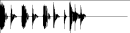
\includegraphics[scale=1]{gen01} 


 Diagram of the waveform generated by GEN01.


 \textbf{Example 1. A simple example of the GEN01 routine.}

\begin{lstlisting}
/* gen01.orc */
; Initialize the global variables.
sr = 44100
kr = 4410
ksmps = 10
nchnls = 1

; Instrument #1.
instr 1
   kamp = 30000
   kcps = 1
   ifn = 1
   ibas = 1

   ; Play the audio sample stored in Table #1.
   a1 loscil kamp, kcps, ifn, ibas
   out a1
endin
/* gen01.orc */
        
\end{lstlisting}
\begin{lstlisting}
/* gen01.sco */
; Table #1: read an audio file (using GEN01).
f 1 0 131072 1 "beats.wav" 0 4 0

; Play Instrument #1 for 2 seconds.
i 1 0 2
e
/* gen01.sco */
        
\end{lstlisting}


  Here is another example of the GEN01 routine. Csound will automatically compute the tablesize because we have set it to 0. This example uses the files \emph{gen01computed.orc}
, \emph{gen01computed.sco}
, and \emph{beats.wav}
. 


 \textbf{Example 2. An example of the GEN01 routine with a computed tablesize.}

\begin{lstlisting}
/* gen01computed.orc */
; Initialize the global variables.
sr = 44100
kr = 4410
ksmps = 10
nchnls = 1

; Instrument #1.
instr 1
   kamp = 30000
   kcps = 1
   ifn = 1
   ibas = 1

   ; Play the audio sample stored in Table #1.
   a1 loscil kamp, kcps, ifn, ibas
   out a1
endin
/* gen01computed.orc */
        
\end{lstlisting}
\begin{lstlisting}
/* gen01computed.sco */
; Table #1: an audio file (using GEN01).
; Since our table size is 0, Csound will compute it.
f 1 0 0 1 "beats.wav" 0 0 0

; Play Instrument #1 for 2 seconds.
i 1 0 2
e
/* gen01computed.sco */
        
\end{lstlisting}
\subsection*{Credits}


 Examples written by Kevin Conder


 December 2002. Thanks goes to Kanata Motohashi for fixing mistakes in the examples.


 September 2003. Thanks goes to Dr. Richard Boulanger for pointing out the references to the AIFF file format. GEN01 also works with WAV files.
%\hline 


\begin{comment}
\begin{tabular}{lcr}
Previous &Home &Next \\
GEN Routines &Up &GEN02

\end{tabular}


\end{document}
\end{comment}

%\begin{comment}
\documentclass[10pt]{article}
\usepackage{fullpage, graphicx, url}
\setlength{\parskip}{1ex}
\setlength{\parindent}{0ex}
\title{GEN02}
\begin{document}


\begin{tabular}{ccc}
The Alternative Csound Reference Manual & & \\
Previous & &Next

\end{tabular}

%\hline 
\end{comment}
\section{GEN02}
GEN02�--� Transfers data from immediate pfields into a function table. \subsection*{Description}


  This subroutine transfers data from immediate pfields into a function table. 
\subsection*{Syntax}


 \textbf{f}
 \# time size 2 v1 v2 v3 ...
\subsection*{Initialization}


 \emph{size}
 -- number of points in the table. Must be a power of 2 or a power-of-2 plus 1 (see \emph{f statement}
). The maximum tablesize is 16777216 (224) points. 


 \emph{v1, v2, v3,}
 etc. -- values to be copied directly into the table space. The number of values is limited by the compile-time variable \emph{PMAX}
, which controls the maximum pfields (currently 1000). The values copied may include the table guard point; any table locations not filled will contain zeros. 


 


\begin{tabular}{cc}
\textbf{Note}
 \\
� &

  If p4 is positive, the table will be post-normalized (rescaled to a maximum absolute value of 1 after generation). A negative p4 will cause rescaling to be skipped. 


\end{tabular}

\subsection*{Examples}


  Here is a simple example of the GEN02 routine. It uses the files \emph{gen02.orc}
 and \emph{gen02.sco}
. It places 12 values plus an explicit wrap-around guard value into a table of size next-highest power of 2. Rescaling is inhibited. Here is its diagram: 


 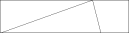
\includegraphics[scale=1]{gen02} 


 Diagram of the waveform generated by GEN02.


 \textbf{Example 1. A simple example of the GEN02 routine.}

\begin{lstlisting}
/* gen02.orc */
; Initialize the global variables.
sr = 44100
kr = 4410
ksmps = 10
nchnls = 1

; Instrument #1.
instr 1
  ; Create an index over the length of our entire note.
  kcps init 1/p3
  kndx phasor kcps

  ; Read Table #1 with our index.
  ifn = 1
  ixmode = 1
  kamp tablei kndx, ifn, ixmode

  ; Create a sine wave, use the Table #1 values to control
  ; the amplitude. This creates a sound with a long attack.
  a1 oscil kamp*30000, 440, 2
  out a1
endin
/* gen02.orc */
        
\end{lstlisting}
\begin{lstlisting}
/* gen02.sco */
; Table #1: an envelope with a long attack (using GEN02).
f 1 0 16 2 0 1 2 3 4 5 6 7 8 9 10 11 0
; Table #2, a sine wave.
f 2 0 16384 10 1

; Play Instrument #1 for 2 seconds.
i 1 0 2
e
/* gen02.sco */
        
\end{lstlisting}
\subsection*{See Also}


 \emph{GEN17}

\subsection*{Credits}


 December 2002. Thanks to Rasmus Ekman, corrected the limit of the \emph{PMAX}
 variable.
%\hline 


\begin{comment}
\begin{tabular}{lcr}
Previous &Home &Next \\
GEN01 &Up &GEN03

\end{tabular}


\end{document}
\end{comment}

%\begin{comment}
\documentclass[10pt]{article}
\usepackage{fullpage, graphicx, url}
\setlength{\parskip}{1ex}
\setlength{\parindent}{0ex}
\title{GEN03}
\begin{document}


\begin{tabular}{ccc}
The Alternative Csound Reference Manual & & \\
Previous & &Next

\end{tabular}

%\hline 
\end{comment}
\section{GEN03}
GEN03�--� Generates a stored function table by evaluating a polynomial. \subsection*{Description}


  This subroutine generates a stored function table by evaluating a polynomial in x over a fixed interval and with specified coefficients. 
\subsection*{Syntax}


 \textbf{f}
 \# time size 3 xval1 xval2 c0 c1 c2 ... cn
\subsection*{Initialization}


 \emph{size }
 -- number of points in the table. Must be a power of 2 or a power-of-2 plus 1. 


 \emph{xval1, xval2 }
 -- left and right values of the x interval over which the polynomial is defined (\emph{xval1}
 $<$ \emph{xval2}
). These will produce the 1st stored value and the (power-of-2 plus l)th stored value respectively in the generated function table. 


 \emph{c0, c1, c2, ... cn}
 -- coefficients of the nth-order polynomial 


 \emph{c0 + c1x + c2x2 + . . . + cnxn}



  Coefficients may be positive or negative real numbers; a zero denotes a missing term in the polynomial. The coefficient list begins in p7, providing a current upper limit of 144 terms. 


 


\begin{tabular}{cc}
\textbf{Note}
 \\
� &

 


 
\begin{itemize}
\item 

  The defined segment [fn(\emph{xval1}
), fn(\emph{xval2}
)] is evenly distributed. Thus a 512-point table over the interval [-1,1] will have its origin at location 257 (at the start of the 2nd half). Provided the extended guard point is requested, both fn(-1) and fn(1) will exist in the table. 

\item 

 \emph{GEN03}
 is useful in conjunction with \emph{table}
 or \emph{tablei}
 for audio waveshaping (sound modification by non-linear distortion). Coefficients to produce a particular formant from a sinusoidal lookup index of known amplitude can be determined at preprocessing time using algorithms such as Chebyshev formulae. See also \emph{GEN13}
. 


\end{itemize}


\end{tabular}

\subsection*{Examples}


  Here is a simple example of the GEN03 routine. It uses the files \emph{gen03.orc}
 and \emph{gen03.sco}
. It fills a table with a 4th order polynomial function over the x-interval -1 to 1. The origin will be at the offset position 512. The function is post-normalized. Here is its diagram: 


 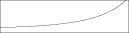
\includegraphics[scale=1]{gen03} 


 Diagram of the waveform generated by GEN03.


 \textbf{Example 1. A simple example of the GEN03 routine.}

\begin{lstlisting}
/* gen03.orc */
; Initialize the global variables.
sr = 44100
kr = 4410
ksmps = 10
nchnls = 1

; Instrument #1.
instr 1
  ; Create an index over the length of our entire note.
  kcps init 1/p3
  kndx phasor kcps

  ; Read Table #1 with our index.
  ifn = 1
  ixmode = 1
  kamp table kndx, ifn, ixmode

  ; Create a sine wave, use the Table #1 values to control
  ; the amplitude.
  a1 oscil kamp*30000, 440, 2
  out a1
endin
/* gen03.orc */
        
\end{lstlisting}
\begin{lstlisting}
/* gen03.sco */
; Table #1: a polynomial function (using GEN03).
f 1 0 1025 3 -1 1 5 4 3 2 2 1
; Table #2, a sine wave.
f 2 0 16384 10 1

; Play Instrument #1 for 2 seconds.
i 1 0 2
e
/* gen03.sco */
        
\end{lstlisting}
\subsection*{See Also}


 \emph{GEN13}
, \emph{GEN14}
, and \emph{GEN15}
. 
%\hline 


\begin{comment}
\begin{tabular}{lcr}
Previous &Home &Next \\
GEN02 &Up &GEN04

\end{tabular}


\end{document}
\end{comment}

%\begin{comment}
\documentclass[10pt]{article}
\usepackage{fullpage, graphicx, url}
\setlength{\parskip}{1ex}
\setlength{\parindent}{0ex}
\title{GEN04}
\begin{document}


\begin{tabular}{ccc}
The Alternative Csound Reference Manual & & \\
Previous & &Next

\end{tabular}

%\hline 
\end{comment}
\section{GEN04}
GEN04�--� Generates a normalizing function. \subsection*{Description}


  This subroutine generates a normalizing function by examining the contents of an existing table. 
\subsection*{Syntax}


 \textbf{f}
 \# time size 4 source\# sourcemode
\subsection*{Initialization}


 \emph{size}
 -- number of points in the table. Should be power-of-2 plus 1. Must not exceed (except by 1) the size of the source table being examined; limited to just half that size if the sourcemode is of type offset (see below). 


 \emph{source \#}
 -- table number of stored function to be examined. 


 \emph{sourcemode}
 -- a coded value, specifying how the source table is to be scanned to obtain the normalizing function. Zero indicates that the source is to be scanned from left to right. Non-zero indicates that the source has a bipolar structure; scanning will begin at the mid-point and progress outwards, looking at pairs of points equidistant from the center. 


 


\begin{tabular}{cc}
\textbf{Note}
 \\
� &

 


 
\begin{itemize}
\item 

  The normalizing function derives from the progressive absolute maxima of the source table being scanned. The new table is created left-to-right, with stored values equal to 1/(absolute maximum so far scanned). Stored values will thus begin with 1/(first value scanned), then get progressively smaller as new maxima are encountered. For a source table which is normalized (values $<$= 1), the derived values will range from 1/(first value scanned) down to 1. If the first value scanned is zero, that inverse will be set to 1. 

\item 

  The normalizing function from \emph{GEN04}
 is not itself normalized. 

\item 

 \emph{GEN04}
 is useful for scaling a table-derived signal so that it has a consistent peak amplitude. A particular application occurs in waveshaping when the carrier (or indexing) signal is less than full amplitude. 


\end{itemize}


\end{tabular}

\subsection*{Examples}


 


 
\begin{lstlisting}
\emph{f}
   2   0   512   4    1   1   
        
\end{lstlisting}


 
 This creates a normalizing function for use in connection with the \emph{GEN03}
 table 1 example. Midpoint bipolar offset is specified. %\hline 


\begin{comment}
\begin{tabular}{lcr}
Previous &Home &Next \\
GEN03 &Up &GEN05

\end{tabular}


\end{document}
\end{comment}

%\begin{comment}
\documentclass[10pt]{article}
\usepackage{fullpage, graphicx, url}
\setlength{\parskip}{1ex}
\setlength{\parindent}{0ex}
\title{GEN05}
\begin{document}


\begin{tabular}{ccc}
The Alternative Csound Reference Manual & & \\
Previous & &Next

\end{tabular}

%\hline 
\end{comment}
\section{GEN05}
GEN05�--� Constructs functions from segments of exponential curves. \subsection*{Description}


  Constructs functions from segments of exponential curves. 
\subsection*{Syntax}


 \textbf{f}
 \# time size 5 a n1 b n2 c ...
\subsection*{Initialization}


 \emph{size }
 -- number of points in the table. Must be a power of 2 or power-of-2 plus 1 (see \emph{f statement}
). 


 \emph{a, b, c,}
 etc. -- ordinate values, in odd-numbered pfields p5, p7, p9, . . . These must be nonzero and must be alike in sign. 


 \emph{n1, n2}
, etc. -- length of segment (no. of storage locations), in even-numbered pfields. Cannot be negative, but a zero is meaningful for specifying discontinuous waveforms (e.g. in the example below). The sum \emph{n1}
 + \emph{n2}
 + .... will normally equal \emph{size}
 for fully specified functions. If the sum is smaller, the function locations not included will be set to zero; if the sum is greater, only the first \emph{size}
 locations will be stored. 


 


\begin{tabular}{cc}
\textbf{Note}
 \\
� &

 


 
\begin{itemize}
\item 

  If p4 is positive, functions are post-normalized (rescaled to a maximum absolute value of 1 after generation). A negative p4 will cause rescaling to be skipped. 

\item 

  Discrete-point linear interpolation implies an increase or decrease along a segment by equal differences between adjacent locations; exponential interpolation implies that the progression is by equal ratio. In both forms the interpolation from \emph{a}
 to \emph{b}
 is such as to assume that the value \emph{b}
 will be attained in the n + 1th location. For discontinuous functions, and for the segment encompassing the end location, this value will not actually be reached, although it may eventually appear as a result of final scaling. 


\end{itemize}


\end{tabular}

\subsection*{Examples}


  Here is a simple example of the GEN05 routine. It uses the files \emph{gen05.orc}
 and \emph{gen05.sco}
. It will create a nice percussive amplitude envelope. Here is its diagram: 


 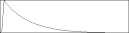
\includegraphics[scale=1]{gen05} 


 Diagram of the waveform generated by GEN05.


 \textbf{Example 1. A simple example of the GEN05 routine.}

\begin{lstlisting}
/* gen05.orc */
; Initialize the global variables.
sr = 44100
kr = 4410
ksmps = 10
nchnls = 1

; Instrument #1.
instr 1
  ; Create an index over the length of our entire note.
  kcps init 1/p3
  kndx phasor kcps

  ; Read Table #1 with our index.
  ifn = 1
  ixmode = 1
  kamp table kndx, ifn, ixmode

  ; Create a sine wave, use the Table #1 values to control
  ; the amplitude. This creates a nice percussive sound.
  a1 oscil kamp*30000, 440, 2
  out a1
endin
/* gen05.orc */
        
\end{lstlisting}
\begin{lstlisting}
/* gen05.sco */
; Table #1: a percussive envelope (using GEN05).
f 1 0 64 5 1 2 120 60 1 1 0.001 1
; Table #2, a sine wave.
f 2 0 16384 10 1

; Play Instrument #1 for 2 seconds.
i 1 0 2
e
/* gen05.sco */
        
\end{lstlisting}
\subsection*{See Also}


 \emph{GEN06}
, \emph{GEN07}
, and \emph{GEN08}

\subsection*{Credits}


 Example written by Kevin Conder
%\hline 


\begin{comment}
\begin{tabular}{lcr}
Previous &Home &Next \\
GEN04 &Up &GEN06

\end{tabular}


\end{document}
\end{comment}

%\begin{comment}
\documentclass[10pt]{article}
\usepackage{fullpage, graphicx, url}
\setlength{\parskip}{1ex}
\setlength{\parindent}{0ex}
\title{GEN06}
\begin{document}


\begin{tabular}{ccc}
The Alternative Csound Reference Manual & & \\
Previous & &Next

\end{tabular}

%\hline 
\end{comment}
\section{GEN06}
GEN06�--� Generates a function comprised of segments of cubic polynomials. \subsection*{Description}


  This subroutine will generate a function comprised of segments of cubic polynomials, spanning specified points just three at a time. 
\subsection*{Syntax}


 \textbf{f}
 \# time size 6 a n1 b n2 c n3 d ...
\subsection*{Initialization}


 \emph{size}
 -- number of points in the table. Must be a power off or power-of-2 plus 1 (see \emph{f statement}
). 


 \emph{a, c, e, ...}
 -- local maxima or minima of successive segments, depending on the relation of these points to adjacent inflexions. May be either positive or negative. 


 \emph{b, d, f, ...}
 -- ordinate values of points of inflexion at the ends of successive curved segments. May be positive or negative. 


 \emph{n1, n2, n3 ...}
 -- number of stored values between specified points. Cannot be negative, but a zero is meaningful for specifying discontinuities. The sum \emph{n1}
 + \emph{n2}
 + ... will normally equal size for fully specified functions. (for details, see \emph{GEN05}
). 


 


\begin{tabular}{cc}
\textbf{Note}
 \\
� &

 \emph{GEN06}
 constructs a stored function from segments of cubic polynomial functions. Segments link ordinate values in groups of 3: point of inflexion, maximum/minimum, point of inflexion. The first complete segment encompasses \emph{b}
, \emph{c}
, \emph{d}
 and has length \emph{n2}
 + \emph{n3}
, the next encompasses \emph{d}
, \emph{e}
, \emph{f}
 and has length \emph{n4}
 + \emph{n5}
, etc. The first segment (\emph{a}
, \emph{b}
 with length \emph{n1}
) is partial with only one inflexion; the last segment may be partial too. Although the inflexion points \emph{b}
, \emph{d}
, \emph{f}
 ... each figure in two segments (to the left and right), the slope of the two segments remains independent at that common point (i.e. the 1st derivative will likely be discontinuous). When \emph{a}
, \emph{c}
, \emph{e}
... are alternately maximum and minimum, the inflexion joins will be relatively smooth; for successive maxima or successive minima the inflexions will be comb-like. 


\end{tabular}

\subsection*{Examples}


  Here is a simple example of the GEN06 routine. It uses the files \emph{gen06.orc}
 and \emph{gen06.sco}
. It creates a curve running 0 to 1 to -1, with a minimum, maximum and minimum at these values respectively. Inflexions are at .5 and 0 and are relatively smooth. Here is its diagram: 


 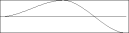
\includegraphics[scale=1]{gen06} 


 Diagram of the waveform generated by GEN06.


 \textbf{Example 1. A simple example of the GEN06 routine.}

\begin{lstlisting}
/* gen06.orc */
; Initialize the global variables.
sr = 44100
kr = 4410
ksmps = 10
nchnls = 1

; Instrument #1.
instr 1
  ; Create an index over the length of our entire note.
  kcps init 1/p3
  kndx phasor kcps

  ; Read Table #1 with our index.
  ifn = 1
  ixmode = 1
  kval table kndx, ifn, ixmode

  ; Generate a sine waveform, use our Table #1 value to 
  ; vary its frequency by 100 Hz from its base frequency.
  ibasefreq = 440
  kfreq = kval * 100
  a1 oscil 20000, ibasefreq + kfreq, 2
  out a1
endin
/* gen06.orc */
        
\end{lstlisting}
\begin{lstlisting}
/* gen06.sco */
; Table #1: a curve (using GEN06).
f 1 0 65 6 0 16 0.5 16 1 16 0 16 -1
; Table #2, a sine wave.
f 2 0 16384 10 1

; Play Instrument #1 for 2 seconds.
i 1 0 2
e
/* gen06.sco */
        
\end{lstlisting}
\subsection*{See Also}


 \emph{GEN05}
, \emph{GEN07}
, and \emph{GEN08}

%\hline 


\begin{comment}
\begin{tabular}{lcr}
Previous &Home &Next \\
GEN05 &Up &GEN07

\end{tabular}


\end{document}
\end{comment}

%\begin{comment}
\documentclass[10pt]{article}
\usepackage{fullpage, graphicx, url}
\setlength{\parskip}{1ex}
\setlength{\parindent}{0ex}
\title{GEN07}
\begin{document}


\begin{tabular}{ccc}
The Alternative Csound Reference Manual & & \\
Previous & &Next

\end{tabular}

%\hline 
\end{comment}
\section{GEN07}
GEN07�--� Constructs functions from segments of straight lines. \subsection*{Description}


  Constructs functions from segments of straight lines. 
\subsection*{Syntax}


 \textbf{f}
 \# time size 7 a n1 b n2 c ...
\subsection*{Initialization}


 \emph{size }
 -- number of points in the table. Must be a power of 2 or power-of-2 plus 1 (see \emph{f statement}
). 


 \emph{a, b, c,}
 etc. -- ordinate values, in odd-numbered pfields p5, p7, p9, . . . 


 \emph{n1, n2}
, etc. -- length of segment (no. of storage locations), in even-numbered pfields. Cannot be negative, but a zero is meaningful for specifying discontinuous waveforms (e.g. in the example below). The sum \emph{n1}
 + \emph{n2}
 + .... will normally equal \emph{size}
 for fully specified functions. If the sum is smaller, the function locations not included will be set to zero; if the sum is greater, only the first \emph{size}
 locations will be stored. 


 


\begin{tabular}{cc}
\textbf{Note}
 \\
� &

 


 
\begin{itemize}
\item 

  If p4 is positive, functions are post-normalized (rescaled to a maximum absolute value of 1 after generation). A negative p4 will cause rescaling to be skipped. 

\item 

  Discrete-point linear interpolation implies an increase or decrease along a segment by equal differences between adjacent locations; exponential interpolation implies that the progression is by equal ratio. In both forms the interpolation from \emph{a}
 to \emph{b}
 is such as to assume that the value \emph{b}
 will be attained in the n + 1th location. For discontinuous functions, and for the segment encompassing the end location, this value will not actually be reached, although it may eventually appear as a result of final scaling. 


\end{itemize}


\end{tabular}

\subsection*{Examples}


  Here is a simple example of the GEN07 routine. It uses the files \emph{gen07.orc}
 and \emph{gen07.sco}
. It will create a single-cycle sawtooth whose discontinuity is mid-way in the stored function. Here is its diagram: 


 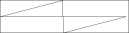
\includegraphics[scale=1]{gen07} 


 Diagram of the waveform generated by GEN07.


 \textbf{Example 1. A simple example of the GEN07 routine.}

\begin{lstlisting}
/* gen07.orc */
; Initialize the global variables.
sr = 44100
kr = 4410
ksmps = 10
nchnls = 1

; Instrument #1.
instr 1
  kamp = 30000
  kcps = 440
  ifn = 1

  ; Play the sine wave stored in Table #1.
  a1 oscil kamp, kcps, ifn
  out a1
endin
/* gen07.orc */
        
\end{lstlisting}
\begin{lstlisting}
/* gen07.sco */
; Table #1: a sawtooth wave (using GEN07).
f 1 0 256 7 0 128 1 0 -1 128 0

; Play Instrument #1 for 2 seconds.
i 1 0 2
e
/* gen07.sco */
        
\end{lstlisting}
\subsection*{See Also}


 \emph{GEN05}
, \emph{GEN06}
, and \emph{GEN08}

%\hline 


\begin{comment}
\begin{tabular}{lcr}
Previous &Home &Next \\
GEN06 &Up &GEN08

\end{tabular}


\end{document}
\end{comment}

%\begin{comment}
\documentclass[10pt]{article}
\usepackage{fullpage, graphicx, url}
\setlength{\parskip}{1ex}
\setlength{\parindent}{0ex}
\title{GEN08}
\begin{document}


\begin{tabular}{ccc}
The Alternative Csound Reference Manual & & \\
Previous & &Next

\end{tabular}

%\hline 
\end{comment}
\section{GEN08}
GEN08�--� Generate a piecewise cubic spline curve. \subsection*{Description}


  This subroutine will generate a piecewise cubic spline curve, the smoothest possible through all specified points. 
\subsection*{Syntax}


 \textbf{f}
 \# time size 8 a n1 b n2 c n3 d ...
\subsection*{Initialization}


 \emph{size}
 -- number of points in the table. Must be a power of 2 or power-of-2 plus 1 (see \emph{f statement}
). 


 \emph{a, b, c,}
 etc. -- ordinate values of the function. 


 \emph{n1, n2, n3 ... }
 -- length of each segment measured in stored values. May not be zero, but may be fractional. A particular segment may or may not actually store any values; stored values will be generated at integral points from the beginning of the function. The sum \emph{n1}
 + \emph{n2}
 + ... will normally equal \emph{size}
 for fully specified functions. 


 


\begin{tabular}{cc}
\textbf{Note}
 \\
� &

 


 
\begin{itemize}
\item 

 \emph{GEN08}
 constructs a stored table from segments of cubic polynomial functions. Each segment runs between two specified points but depends as well on their neighbors on each side. Neighboring segments will agree in both value and slope at their common point. (The common slope is that of a parabola through that point and its two neighbors). The slope at the two ends of the function is constrained to be zero (flat). 

\item 

 \emph{Hint:}
 to make a discontinuity in slope or value in the function as stored, arrange a series of points in the interval between two stored values; likewise for a non-zero boundary slope. 


\end{itemize}


\end{tabular}

\subsection*{Examples}


  Here is a simple example of the GEN08 routine. It uses the files \emph{gen08.orc}
 and \emph{gen08.sco}
. It will create a curve with a smooth hump in the middle, going briefly negative outside the hump then flat at its ends. Here is its diagram: 


 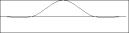
\includegraphics[scale=1]{gen08} 


 Diagram of the waveform generated by GEN08.


 \textbf{Example 1. A simple example of the GEN08 routine.}

\begin{lstlisting}
/* gen08.orc */
; Initialize the global variables.
sr = 44100
kr = 4410
ksmps = 10
nchnls = 1

; Instrument #1.
instr 1
  ; Create an index over the length of our entire note.
  kcps init 1/p3
  kndx phasor kcps

  ; Read Table #1 with our index.
  ifn = 1
  ixmode = 1
  kval table kndx, ifn, ixmode

  ; Generate a sine waveform, use our Table #1 value to 
  ; vary its frequency by 100 Hz from its base frequency.
  ibasefreq = 440
  kfreq = kval * 100
  a1 oscil 20000, ibasefreq + kfreq, 2
  out a1
endin
/* gen08.orc */
        
\end{lstlisting}
\begin{lstlisting}
/* gen08.sco */
; Table #1: a curve with a smooth hump (using GEN08).
f 1 0 65 8 0 16 0 16 1 16 0 16 0
; Table #2, a sine wave.
f 2 0 16384 10 1

; Play Instrument #1 for two seconds.
i 1 0 2
e
/* gen08.sco */
        
\end{lstlisting}
\subsection*{See Also}


 \emph{GEN05}
, \emph{GEN06}
, and \emph{GEN07}

%\hline 


\begin{comment}
\begin{tabular}{lcr}
Previous &Home &Next \\
GEN07 &Up &GEN09

\end{tabular}


\end{document}
\end{comment}

%\begin{comment}
\documentclass[10pt]{article}
\usepackage{fullpage, graphicx, url}
\setlength{\parskip}{1ex}
\setlength{\parindent}{0ex}
\title{GEN09}
\begin{document}


\begin{tabular}{ccc}
The Alternative Csound Reference Manual & & \\
Previous & &Next

\end{tabular}

%\hline 
\end{comment}
\section{GEN09}
GEN09�--� Generate composite waveforms made up of weighted sums of simple sinusoids. \subsection*{Description}


  These subroutines generate composite waveforms made up of weighted sums of simple sinusoids. The specification of each contributing partial requires 3 p-fields using \emph{GEN09}
. 
\subsection*{Syntax}


 \textbf{f}
 \# time size 9 pna stra phsa pnb strb phsb ...
\subsection*{Initialization}


 \emph{size}
 -- number of points in the table. Must be a power of 2 or power-of-2 plus 1 (see \emph{f statement}
). 


 \emph{pna, pnb}
, etc. -- partial no. (relative to a fundamental that would occupy \emph{size}
 locations per cycle) of sinusoid a, sinusoid b, etc. Must be positive, but need not be a whole number, i.e., non-harmonic partials are permitted. Partials may be in any order. 


 \emph{stra, strb}
, etc. -- strength of partials \emph{pna, pnb}
, etc. These are relative strengths, since the composite waveform may be rescaled later. Negative values are permitted and imply a 180 degree phase shift. 


 \emph{phsa, phsb}
, etc. -- initial phase of partials \emph{pna, pnb,}
 etc., expressed in degrees (0-360). 


 


\begin{tabular}{cc}
\textbf{Note}
 \\
� &

 


 
\begin{itemize}
\item 

  These subroutines generate stored functions as sums of sinusoids of different frequencies. The two major restrictions on \emph{GEN10}
 that the partials be harmonic and in phase do not apply to \emph{GEN09}
 or \emph{GEN19}
. 


  In each case the composite wave, once drawn, is then rescaled to unity if p4 was positive. A negative p4 will cause rescaling to be skipped. 


\end{itemize}


\end{tabular}

\subsection*{Examples}


  Here is a simple example of the GEN09 routine. It uses the files \emph{gen09.orc}
 and \emph{gen09.sco}
. It will generate a cosine wave, a sine wave with an initial phase of 90 degrees. Here is its diagram: 


 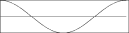
\includegraphics[scale=1]{gen09} 


 Diagram of the waveform generated by GEN09.


 \textbf{Example 1. A simple example of the GEN09 routine.}

\begin{lstlisting}
/* gen09.orc */
; Initialize the global variables.
sr = 44100
kr = 4410
ksmps = 10
nchnls = 1

; Instrument #1.
instr 1
  kamp = 30000
  kcps = 440
  ifn = 1

  ; Play the waveform stored in Table #1.
  a1 oscil kamp, kcps, ifn
  out a1
endin
/* gen09.orc */
        
\end{lstlisting}
\begin{lstlisting}
/* gen09.sco */
; Table #1: a cosine wave (using GEN09).
; This is a sine wave with an initial phase of 90 degrees.
f 1 0 16384 9 1 1 90

; Play Instrument #1 for 2 seconds.
i 1 0 2
e
/* gen09.sco */
        
\end{lstlisting}


  Here is another example of the GEN09 routine. It uses the files \emph{gen09square.orc}
 and \emph{gen09square.sco}
. It combines partials l, 3 and 9 in the relative strengths in which they are found in a square wave, except that partial 9 is upside down. It will be rescaled, here is its diagram: 


 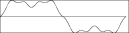
\includegraphics[scale=1]{gen09square} 


 Diagram of the waveform generated by GEN09.


 \textbf{Example 2. A square wave generated by the GEN09 routine.}

\begin{lstlisting}
/* gen09square.orc */
; Initialize the global variables.
sr = 44100
kr = 4410
ksmps = 10
nchnls = 1

; Instrument #1.
instr 1
  kamp = 30000
  kcps = 440
  ifn = 1

  ; Play the waveform stored in Table #1.
  a1 oscil kamp, kcps, ifn
  out a1
endin
/* gen09square.orc */
        
\end{lstlisting}
\begin{lstlisting}
/* gen09square.sco */
; Table #1: an approximation of a square wave (using GEN09).
f 1 0 16384 9 1 3 0 3 1 0 9 0.3333 180

; Play Instrument #1 for 2 seconds.
i 1 0 2
e
/* gen09square.sco */
        
\end{lstlisting}
\subsection*{See Also}


 \emph{GEN10}
, \emph{GEN19}

\subsection*{Credits}


 The simple example was written by Kevin Conder.
%\hline 


\begin{comment}
\begin{tabular}{lcr}
Previous &Home &Next \\
GEN08 &Up &GEN10

\end{tabular}


\end{document}
\end{comment}

%\begin{comment}
\documentclass[10pt]{article}
\usepackage{fullpage, graphicx, url}
\setlength{\parskip}{1ex}
\setlength{\parindent}{0ex}
\title{GEN10}
\begin{document}


\begin{tabular}{ccc}
The Alternative Csound Reference Manual & & \\
Previous & &Next

\end{tabular}

%\hline 
\end{comment}
\section{GEN10}
GEN10�--� Generate composite waveforms made up of weighted sums of simple sinusoids. \subsection*{Description}


  These subroutines generate composite waveforms made up of weighted sums of simple sinusoids. The specification of each contributing partial requires 1 pfield using \emph{GEN10}
. 
\subsection*{Syntax}


 \textbf{f}
 \# time size 10 str1 str2 str3 str4 ...
\subsection*{Initialization}


 \emph{size}
 -- number of points in the table. Must be a power of 2 or power-of-2 plus 1 (see \emph{f statement}
). 


 \emph{str1, str2, str3, etc.}
 -- relative strengths of the fixed harmonic partial numbers 1,2,3, etc., beginning in p5. Partials not required should be given a strength of zero. 


 


\begin{tabular}{cc}
\textbf{Note}
 \\
� &

 


 
\begin{itemize}
\item 

  These subroutines generate stored functions as sums of sinusoids of different frequencies. The two major restrictions on \emph{GEN10}
 that the partials be harmonic and in phase do not apply to \emph{GEN09}
 or \emph{GEN19}
. 


  In each case the composite wave, once drawn, is then rescaled to unity if p4 was positive. A negative p4 will cause rescaling to be skipped. 


\end{itemize}


\end{tabular}

\subsection*{Examples}


  Here is a simple example of the GEN10 routine. It uses the files \emph{gen10.orc}
 and \emph{gen10.sco}
. It will generate a simple sine wave. Here is its diagram: 


 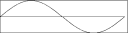
\includegraphics[scale=1]{gen10} 


 Diagram of the waveform generated by GEN10.


 \textbf{Example 1. A simple example of the GEN10 routine.}

\begin{lstlisting}
/* gen10.orc */
; Initialize the global variables.
sr = 44100
kr = 4410
ksmps = 10
nchnls = 1

; Instrument #1.
instr 1
  kamp = 30000
  kcps = 440
  ifn = 1

  ; Play the sine wave stored in Table #1.
  a1 oscil kamp, kcps, ifn
  out a1
endin
/* gen10.orc */
        
\end{lstlisting}
\begin{lstlisting}
/* gen10.sco */
; Table #1: a simple sine wave (using GEN10).
f 1 0 16384 10 1

; Play Instrument #1 for 2 seconds.
i 1 0 2
e
/* gen10.sco */
        
\end{lstlisting}
\subsection*{See Also}


 \emph{GEN09}
, \emph{GEN11}
, and \emph{GEN19}
. 
\subsection*{Credits}


 Example written by Kevin Conder
%\hline 


\begin{comment}
\begin{tabular}{lcr}
Previous &Home &Next \\
GEN09 &Up &GEN11

\end{tabular}


\end{document}
\end{comment}

%\begin{comment}
\documentclass[10pt]{article}
\usepackage{fullpage, graphicx, url}
\setlength{\parskip}{1ex}
\setlength{\parindent}{0ex}
\title{GEN11}
\begin{document}


\begin{tabular}{ccc}
The Alternative Csound Reference Manual & & \\
Previous & &Next

\end{tabular}

%\hline 
\end{comment}
\section{GEN11}
GEN11�--� Generates an additive set of cosine partials. \subsection*{Description}


  This subroutine generates an additive set of cosine partials, in the manner of Csound generators \emph{buzz}
 and \emph{gbuzz}
. 
\subsection*{Syntax}


 \textbf{f}
 \# time size 11 nh [lh] [r]
\subsection*{Initialization}


 \emph{size}
 -- number of points in the table. Must be a power of 2 or power-of-2 plus 1 (see \emph{f statement}
). 


 \emph{nh}
 -- number of harmonics requested. Must be positive. 


 \emph{lh}
(optional) -- lowest harmonic partial present. Can be positive, zero or negative. The set of partials can begin at any partial number and proceeds upwards; if \emph{lh}
 is negative, all partials below zero will reflect in zero to produce positive partials without phase change (since cosine is an even function), and will add constructively to any positive partials in the set. The default value is 1 


 \emph{r}
(optional) -- multiplier in an amplitude coefficient series. This is a power series: if the \emph{lh}
th partial has a strength coefficient of A the (\emph{lh}
 + n)th partial will have a coefficient of A * rn, i.e. strength values trace an exponential curve. \emph{r}
 may be positive, zero or negative, and is not restricted to integers. The default value is 1. 


 


\begin{tabular}{cc}
\textbf{Note}
 \\
� &

 


 
\begin{itemize}
\item 

  This subroutine is a non-time-varying version of the CSound \emph{buzz}
and \emph{gbuzz}
 generators, and is similarly useful as a complex sound source in subtractive synthesis. With \emph{lh}
 and \emph{r}
 present it parallels \emph{gbuzz}
; with both absent or equal to 1 it reduces to the simpler \emph{buzz}
 (i.e. \emph{nh}
 equal-strength harmonic partials beginning with the fundamental). 

\item 

  Sampling the stored waveform with an oscillator is more efficient than using the dynamic buzz units. However, the spectral content is invariant and care is necessary, lest the higher partials exceed the Nyquist during sampling to produce fold-over. 


\end{itemize}


\end{tabular}

\subsection*{Examples}


  Here is a simple example of the GEN11 routine. It uses the files \emph{gen11.orc}
 and \emph{gen11.sco}
. It will generate a simple cosine wave. Here is its diagram: 


 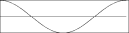
\includegraphics[scale=1]{gen11} 


 Diagram of the waveform generated by GEN11.


 \textbf{Example 1. A simple example of the GEN11 routine.}

\begin{lstlisting}
/* gen11.orc */
; Initialize the global variables.
sr = 44100
kr = 4410
ksmps = 10
nchnls = 1

; Instrument #1.
instr 1
  kamp = 30000
  kcps = 440
  ifn = 1

  ; Play the cosine wave stored in Table #1.
  a1 oscil kamp, kcps, ifn
  out a1
endin
/* gen11.orc */
        
\end{lstlisting}
\begin{lstlisting}
/* gen11.sco */
; Table #1: a simple cosine wave (using GEN11).
f 1 0 16384 11 1 1

; Play Instrument #1 for 2 seconds.
i 1 0 2
e
/* gen11.sco */
        
\end{lstlisting}
\subsection*{See Also}


 \emph{GEN10}

\subsection*{Credits}


 Example written by Kevin Conder
%\hline 


\begin{comment}
\begin{tabular}{lcr}
Previous &Home &Next \\
GEN10 &Up &GEN12

\end{tabular}


\end{document}
\end{comment}

%\begin{comment}
\documentclass[10pt]{article}
\usepackage{fullpage, graphicx, url}
\setlength{\parskip}{1ex}
\setlength{\parindent}{0ex}
\title{GEN12}
\begin{document}


\begin{tabular}{ccc}
The Alternative Csound Reference Manual & & \\
Previous & &Next

\end{tabular}

%\hline 
\end{comment}
\section{GEN12}
GEN12�--� Generates the log of a modified Bessel function of the second kind. \subsection*{Description}


  This generates the log of a modified Bessel function of the second kind, order 0, suitable for use in amplitude-modulated FM. 
\subsection*{Syntax}


 \textbf{f}
 \# time size 12 xint
\subsection*{Initialization}


 \emph{size }
 -- number of points in the table. Must be a power of 2 or a power-of-2 plus 1 (see \emph{f statement}
). The normal value is power-of-2 plus 1. 


 \emph{xint}
 -- specifies the \emph{x}
 interval [0 to \emph{+xint}
] over which the function is defined. 


 


\begin{tabular}{cc}
\textbf{Note}
 \\
� &

 


 
\begin{itemize}
\item 

  This subroutine draws the natural log of a modified Bessel function of the second kind, order 0 (commonly written as \emph{I}
 subscript 0), over the x-interval requested. The call should have rescaling inhibited. 

\item 

  The function is useful as an amplitude scaling factor in cycle-synchronous amplitude-modulated FM. (See Palamin \& Palamin, \emph{J. Audio Eng. Soc., 36/9}
, Sept. 1988, pp.671-684.) The algorithm is interesting because it permits the normally symmetric FM spectrum to be made asymmetric around a frequency other than the carrier, and is thereby useful for formant positioning. By using a table lookup index of \emph{I}
(r - 1/r), where \emph{I}
 is the FM modulation index and \emph{r}
 is an exponential parameter affecting partial strengths, the Palamin algorithm becomes relatively efficient, requiring only oscil's, table lookups, and a single \emph{exp}
 call. 


\end{itemize}


\end{tabular}

\subsection*{Examples}


  Here is a simple example of the GEN12 routine. It uses the files \emph{gen12.orc}
 and \emph{gen12.sco}
. It generates the function \emph{ln(I0(x))}
 from 0 to 20. Here is its diagram: 


 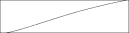
\includegraphics[scale=1]{gen12} 


 Diagram of the waveform generated by GEN12.


 \textbf{Example 1. A simple example of the GEN12 routine.}

\begin{lstlisting}
/* gen12.orc */
; Initialize the global variables.
sr = 44100
kr = 4410
ksmps = 10
nchnls = 1

; Instrument #1.
instr 1
  ; Create an index over the length of our entire note.
  kcps init 1/p3
  kndx phasor kcps

  ; Read Table #1 with our index.
  ifn = 1
  ixmode = 1
  kamp tablei kndx, ifn, ixmode

  ; Create a sine wave, use the Table #1 values to control
  ; the amplitude. This creates a sound with a long attack.
  a1 oscil kamp*30000, 440, 2
  out a1
endin
/* gen12.orc */
        
\end{lstlisting}
\begin{lstlisting}
/* gen12.sco */
; Table #1: a modified Bessel function (using GEN12).
f 1 0 2049 12 20
; Table #2, a sine wave.
f 2 0 16384 10 1

; Play Instrument #1 for 2 seconds.
i 1 0 2
e
/* gen12.sco */
        
\end{lstlisting}
\subsection*{Credits}


 Example written by Kevin Conder
%\hline 


\begin{comment}
\begin{tabular}{lcr}
Previous &Home &Next \\
GEN11 &Up &GEN13

\end{tabular}


\end{document}
\end{comment}

%\begin{comment}
\documentclass[10pt]{article}
\usepackage{fullpage, graphicx, url}
\setlength{\parskip}{1ex}
\setlength{\parindent}{0ex}
\title{GEN13}
\begin{document}


\begin{tabular}{ccc}
The Alternative Csound Reference Manual & & \\
Previous & &Next

\end{tabular}

%\hline 
\end{comment}
\section{GEN13}
GEN13�--� Stores a polynomial whose coefficients derive from the Chebyshev polynomials of the first kind. \subsection*{Description}


  Uses Chebyshev coefficients to generate stored polynomial functions which, under waveshaping, can be used to split a sinusoid into harmonic partials having a pre-definable spectrum. 
\subsection*{Syntax}


 \textbf{f}
 \# time size 13 xint xamp h0 h1 h2 ...
\subsection*{Initialization}


 \emph{size}
 -- number of points in the table. Must be a power of 2 or a power-of-2 plus 1 (see \emph{f statement}
). The normal value is power-of-2 plus 1. 


 \emph{xint}
 -- provides the left and right values [\emph{-xint, +xint}
] of the x interval over which the polynomial is to be drawn. These subroutines both call \emph{GEN03}
 to draw their functions; the p5 value here is therefor expanded to a negative-positive p5, p6 pair before \emph{GEN03}
 is actually called. The normal value is 1. 


 \emph{xamp }
 -- amplitude scaling factor of the sinusoid input that is expected to produce the following spectrum. 


 \emph{h0, h1, h2,}
 etc. -- relative strength of partials 0 (DC), 1 (fundamental), 2 ... that will result when a sinusoid of amplitude 


 xamp�*�int(size/2)/xint\\ 
 ������
 is waveshaped using this function table. These values thus describe a frequency spectrum associated with a particular factor \emph{xamp}
 of the input signal. 

 \emph{GEN13}
 is the function generator normally employed in standard waveshaping. It stores a polynomial whose coefficients derive from the Chebyshev polynomials of the first kind, so that a driving sinusoid of strength \emph{xamp}
 will exhibit the specified spectrum at output. Note that the evolution of this spectrum is generally not linear with varying \emph{xamp}
. However, it is bandlimited (the only partials to appear will be those specified at generation time); and the partials will tend to occur and to develop in ascending order (the lower partials dominating at low \emph{xamp}
, and the spectral richness increasing for higher values of \emph{xamp}
). A negative \emph{hn}
 value implies a 180 degree phase shift of that partial; the requested full-amplitude spectrum will not be affected by this shift, although the evolution of several of its component partials may be. The pattern +,+,-,-,+,+,... for \emph{h0,h1,h2..}
. will minimize the normalization problem for low \emph{xamp}
 values (see above), but does not necessarily provide the smoothest pattern of evolution. 
\subsection*{Examples}


  Here is a simple example of the GEN13 routine. It uses the files \emph{gen13.orc}
 and \emph{gen13.sco}
. It creates a function which, under waveshaping, will split a sinusoid into 3 odd-harmonic partials of relative strength 5:3:1. Here is its diagram: 


 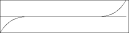
\includegraphics[scale=1]{gen13} 


 Diagram of the waveform generated by GEN13.


 \textbf{Example 1. A simple example of the GEN13 routine.}

\begin{lstlisting}
/* gen13.orc */
; Initialize the global variables.
sr = 44100
kr = 4410
ksmps = 10
nchnls = 1

; Instrument #1.
instr 1
  ; Create an index over the length of our entire note.
  kcps init 1/p3
  kndx phasor kcps

  ; Read Table #1 with our index.
  ifn = 1
  ixmode = 1
  kval table kndx, ifn, ixmode

  ; Generate a sine waveform, use our Table #1 value to
  ; vary its frequency by 100 Hz from its base frequency.
  ibasefreq = 440
  kfreq = kval * 100
  a1 oscil 20000, ibasefreq + kfreq, 2
  out a1
endin
/* gen13.orc */
        
\end{lstlisting}
\begin{lstlisting}
/* gen13.sco */
; Table #1: a polynomial function (using GEN13).
f 1 0 1025 13 1 1 0 5 0 3 0 1
; Table #2, a sine wave.
f 2 0 16384 10 1

; Play Instrument #1 for 2 seconds.
i 1 0 2
e
/* gen13.sco */
        
\end{lstlisting}
\subsection*{See Also}


 \emph{GEN03}
, \emph{GEN14}
, and \emph{GEN15}
. 
%\hline 


\begin{comment}
\begin{tabular}{lcr}
Previous &Home &Next \\
GEN12 &Up &GEN14

\end{tabular}


\end{document}
\end{comment}

%\begin{comment}
\documentclass[10pt]{article}
\usepackage{fullpage, graphicx, url}
\setlength{\parskip}{1ex}
\setlength{\parindent}{0ex}
\title{GEN14}
\begin{document}


\begin{tabular}{ccc}
The Alternative Csound Reference Manual & & \\
Previous & &Next

\end{tabular}

%\hline 
\end{comment}
\section{GEN14}
GEN14�--� Stores a polynomial whose coefficients derive from Chebyshevs of the second kind. \subsection*{Description}


  Uses Chebyshev coefficients to generate stored polynomial functions which, under waveshaping, can be used to split a sinusoid into harmonic partials having a pre-definable spectrum. 
\subsection*{Syntax}


 \textbf{f}
 \# time size 14 xint xamp h0 h1 h2 ...
\subsection*{Initialization}


 \emph{size}
 -- number of points in the table. Must be a power of 2 or a power-of-2 plus 1 (see \emph{f statement}
). The normal value is power-of-2 plus 1. 


 \emph{xint}
 -- provides the left and right values [\emph{-xint, +xint}
] of the x interval over which the polynomial is to be drawn. These subroutines both call \emph{GEN03}
 to draw their functions; the p5 value here is therefore expanded to a negative-positive p5, p6 pair before \emph{GEN03}
 is actually called. The normal value is 1. 


 \emph{xamp }
 -- amplitude scaling factor of the sinusoid input that is expected to produce the following spectrum. 


 \emph{h0, h1, h2,}
 etc. -- relative strength of partials 0 (DC), 1 (fundamental), 2 ... that will result when a sinusoid of amplitude 


 xamp�*�int(size/2)/xint\\ 
 ������
 is waveshaped using this function table. These values thus describe a frequency spectrum associated with a particular factor \emph{xamp}
 of the input signal. 

 


\begin{tabular}{cc}
\textbf{Note}
 \\
� &

 


 
\begin{itemize}
\item 

 \emph{GEN13}
 is the function generator normally employed in standard waveshaping. It stores a polynomial whose coefficients derive from the Chebyshev polynomials of the first kind, so that a driving sinusoid of strength \emph{xamp}
 will exhibit the specified spectrum at output. Note that the evolution of this spectrum is generally not linear with varying \emph{xamp}
. However, it is bandlimited (the only partials to appear will be those specified at generation time); and the partials will tend to occur and to develop in ascending order (the lower partials dominating at low \emph{xamp}
, and the spectral richness increasing for higher values of \emph{xamp}
). A negative \emph{hn}
 value implies a 180 degree phase shift of that partial; the requested full-amplitude spectrum will not be affected by this shift, although the evolution of several of its component partials may be. The pattern +,+,-,-,+,+,... for \emph{h0,h1,h2..}
. will minimize the normalization problem for low \emph{xamp}
 values (see above), but does not necessarily provide the smoothest pattern of evolution. 

\item 

 \emph{GEN14}
 stores a polynomial whose coefficients derive from Chebyshevs of the second kind. 


\end{itemize}


\end{tabular}

\subsection*{Examples}


  Here is a simple example of the GEN14 routine. It uses the files \emph{gen14.orc}
 and \emph{gen14.sco}
. It creates a function which, under waveshaping, will split a sinusoid into 3 odd-harmonic partials of relative strength 5:3:1. Here is its diagram: 


 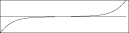
\includegraphics[scale=1]{gen14} 


 Diagram of the waveform generated by GEN14.


 \textbf{Example 1. A simple example of the GEN14 routine.}

\begin{lstlisting}
/* gen14.orc */
; Initialize the global variables.
sr = 44100
kr = 4410
ksmps = 10
nchnls = 1

; Instrument #1.
instr 1
  ; Create an index over the length of our entire note.
  kcps init 1/p3
  kndx phasor kcps

  ; Read Table #1 with our index.
  ifn = 1
  ixmode = 1
  kval table kndx, ifn, ixmode

  ; Generate a sine waveform, use our Table #1 value to
  ; vary its frequency by 100 Hz from its base frequency.
  ibasefreq = 440
  kfreq = kval * 100
  a1 oscil 20000, ibasefreq + kfreq, 2
  out a1
endin
/* gen14.orc */
        
\end{lstlisting}
\begin{lstlisting}
/* gen14.sco */
; Table #1: a polynomial function (using GEN14).
f 1 0 1025 14 1 1 0 5 0 3 0 1
; Table #2, a sine wave.
f 2 0 16384 10 1

; Play Instrument #1 for 2 seconds.
i 1 0 2
e
/* gen14.sco */
        
\end{lstlisting}
\subsection*{See Also}


 \emph{GEN03}
, \emph{GEN13}
, and \emph{GEN15}
. 
\subsection*{Credits}


 Example written by Kevin Conder
%\hline 


\begin{comment}
\begin{tabular}{lcr}
Previous &Home &Next \\
GEN13 &Up &GEN15

\end{tabular}


\end{document}
\end{comment}

%\begin{comment}
\documentclass[10pt]{article}
\usepackage{fullpage, graphicx, url}
\setlength{\parskip}{1ex}
\setlength{\parindent}{0ex}
\title{GEN15}
\begin{document}


\begin{tabular}{ccc}
The Alternative Csound Reference Manual & & \\
Previous & &Next

\end{tabular}

%\hline 
\end{comment}
\section{GEN15}
GEN15�--� Creates two tables of stored polynomial functions. \subsection*{Description}


  This subroutine creates two tables of stored polynomial functions, suitable for use in phase quadrature operations. 
\subsection*{Syntax}


 \textbf{f}
 \# time size 15 xint xamp h0 phs0 h1 phs1 h2 phs2 ...
\subsection*{Initialization}


 \emph{size}
 -- number of points in the table. Must be a power of 2 or a power-of-2 plus 1 (see \emph{f statement}
). The normal value is power-of-2 plus 1. 


 \emph{xint}
 -- provides the left and right values [\emph{-xint}
, \emph{+xint}
] of the \emph{x}
 interval over which the polynomial is to be drawn. This subroutine will eventually call \emph{GEN03}
 to draw both functions; this p5 value is therefor expanded to a negative-positive p5, p6 pair before \emph{GEN03}
 is actually called. The normal value is 1. 


 \emph{xamp }
 -- amplitude scaling factor of the sinusoid input that is expected to produce the following spectrum. 


 \emph{h0, h1, h2, ... hn}
 -- relative strength of partials 0 (DC), 1 (fundamental), 2 ... that will result when a sinusoid of amplitude 


 xamp�*�int(size/2)/xint\\ 
 ������
 is waveshaped using this function table. These values thus describe a frequency spectrum associated with a particular factor \emph{xamp}
 of the input signal. 

 \emph{phs0, phs1, ... }
 -- phase in degrees of desired harmonics \emph{h0, h1, ...}
 when the two functions of \emph{GEN15}
 are used with phase quadrature. 


 


\begin{tabular}{cc}
\textbf{Note}
 \\
� &

 \emph{GEN15}
 creates two tables of equal size, labeled \emph{f }
\# and \emph{f}
 \# + 1. Table \# will contain a Chebyshev function of the first kind, drawn using \emph{GEN03}
 with partial strengths \emph{h0cos(phs0), h1cos(phs1), ...}
 Table \#+1 will contain a Chebyshev function of the 2nd kind by calling \emph{GEN14}
 with partials \emph{h1sin(phs1), h2sin(phs2),...}
 (note the harmonic displacement). The two tables can be used in conjunction in a waveshaping network that exploits phase quadrature. 


\end{tabular}

\subsection*{See Also}


 \emph{GEN03}
, \emph{GEN13}
, and \emph{GEN14}
. 
%\hline 


\begin{comment}
\begin{tabular}{lcr}
Previous &Home &Next \\
GEN14 &Up &GEN16

\end{tabular}


\end{document}
\end{comment}

%\begin{comment}
\documentclass[10pt]{article}
\usepackage{fullpage, graphicx, url}
\setlength{\parskip}{1ex}
\setlength{\parindent}{0ex}
\title{GEN16}
\begin{document}


\begin{tabular}{ccc}
The Alternative Csound Reference Manual & & \\
Previous & &Next

\end{tabular}

%\hline 
\end{comment}
\section{GEN16}
GEN16�--� Creates a table from a starting value to an ending value. \subsection*{Description}


  Creates a table from \emph{beg}
 value to \emph{end}
 value of \emph{dur}
 steps. 
\subsection*{Syntax}


 \textbf{f}
 \# time size 16 beg dur type end
\subsection*{Initialization}


 \emph{size}
 -- number of points in the table. Must be a power of 2 or a power-of-2 plus 1 (see \emph{f statement}
). The normal value is power-of-2 plus 1. 


 \emph{beg}
 -- starting value 


 \emph{dur}
 -- number of segments 


 \emph{type}
 -- if 0, a straight line is produced. If non-zero, then \emph{GEN16}
 creates the following curve, for \emph{dur}
 steps: 


 beg�+�(end�-�beg)�*�(1�-�exp(�i*type/(dur-1)�))�/�(1�-�exp(type))\\ 
 ������


 \emph{end}
 -- value after \emph{dur}
 segments 


 


\begin{tabular}{cc}
\textbf{Note}
 \\
� &

  If \emph{type}
 $>$ 0, there is a slowly rising, fast decaying (convex) curve, while if \emph{type}
 $<$ 0, the curve is fast rising, slowly decaying (concave). See also \emph{transeg}
. 


\end{tabular}

\subsection*{Credits}


 


 


\begin{tabular}{cccc}
Author: John ffitch &University of Bath, Codemist. Ltd. &Bath, UK &October, 2000

\end{tabular}



 


 New in Csound version 4.09
%\hline 


\begin{comment}
\begin{tabular}{lcr}
Previous &Home &Next \\
GEN15 &Up &GEN17

\end{tabular}


\end{document}
\end{comment}

%\begin{comment}
\documentclass[10pt]{article}
\usepackage{fullpage, graphicx, url}
\setlength{\parskip}{1ex}
\setlength{\parindent}{0ex}
\title{GEN17}
\begin{document}


\begin{tabular}{ccc}
The Alternative Csound Reference Manual & & \\
Previous & &Next

\end{tabular}

%\hline 
\end{comment}
\section{GEN17}
GEN17�--� Creates a step function from given x-y pairs. \subsection*{Description}


  This subroutine creates a step function from given x-y pairs. 
\subsection*{Syntax}


 \textbf{f}
 \# time size 17 x1 a x2 b x3 c ...
\subsection*{Initialization}


 \emph{size}
 -- number of points in the table. Must be a power of 2 or a power-of-2 plus 1 (see \emph{f statement}
). The normal value is power-of-2 plus 1. 


 \emph{x1, x2, x3,}
 etc. -- x-ordinate values, in ascending order, 0 first. 


 \emph{a, b, c,}
 etc. -- y-values at those x-ordinates, held until the next x-ordinate. 


 


\begin{tabular}{cc}
\textbf{Note}
 \\
� &

  This subroutine creates a step function of x-y pairs whose y-values are held to the right. The right-most y-value is then held to the end of the table. The function is useful for mapping one set of data values onto another, such as MIDI note numbers onto sampled sound ftable numbers ( see \emph{loscil}
). 


\end{tabular}

\subsection*{Examples}


 


 
\begin{lstlisting}
\emph{f}
  1  0  128  -17   0  1   12  2   24  3   36  4   48  5  60  6   72  7   84  8
        
\end{lstlisting}


 
 This describes a step function with 8 successively increasing levels, each 12 locations wide except the last which extends its value to the end of the table. Rescaling is inhibited. Indexing into this table with a MIDI note-number would retrieve a different value every octave up to the eighth, above which the value returned would remain the same. \subsection*{See Also}


 \emph{GEN02}

%\hline 


\begin{comment}
\begin{tabular}{lcr}
Previous &Home &Next \\
GEN16 &Up &GEN18

\end{tabular}


\end{document}
\end{comment}

%\begin{comment}
\documentclass[10pt]{article}
\usepackage{fullpage, graphicx, url}
\setlength{\parskip}{1ex}
\setlength{\parindent}{0ex}
\title{GEN18}
\begin{document}


\begin{tabular}{ccc}
The Alternative Csound Reference Manual & & \\
Previous & &Next

\end{tabular}

%\hline 
\end{comment}
\section{GEN18}
GEN18�--� Writes composite waveforms made up of pre-existing waveforms. \subsection*{Description}


  Writes composite waveforms made up of pre-existing waveforms. Each contributing waveform requires 4 pfields and can overlap with other waveforms. 
\subsection*{Syntax}


 \textbf{f}
 \# time size 18 fna ampa starta finisha fna ampa starta finisha ...
\subsection*{Initialization}


 \emph{size}
 -- number of points in the table. Must be a power-of-2 plus 1 (see f statement). 


 \emph{fna, fnb, etc.}
 -- pre-existing table number to be written into the table. 


 \emph{ampa, ampb, etc.}
 -- strength of wavefoms. These are relative strengths, since the composite waveform may be rescaled later. Negative values are permitted and imply a 180 degree phase shift. 


 \emph{starta, startb, etc.}
 -- where to start writing the fn into the table. 


 \emph{finisha, finishb, etc.}
 -- where to stop writing the fn into the table. 
\subsection*{Examples}


 


 
\begin{lstlisting}
f 1  0  4096  10  1
f 2  0  1025  18  1  1  0  512  1  1  513  1025
        
\end{lstlisting}


 
 f2 consists of two copies of f1 written in to locations 0-512 and 513-1025. \subsection*{Deprecated Names}


 \emph{GEN18}
 was called \emph{GEN22}
 in version 4.18. The name was changed due to a conflict with DirectCsound. 
\subsection*{Credits}


 


 


\begin{tabular}{cccc}
Author: William ``Pete'' Moss &University of Texas at Austin &Austin, Texas USA &January 2002

\end{tabular}



 


 New in version 4.18, changed in version 4.19
%\hline 


\begin{comment}
\begin{tabular}{lcr}
Previous &Home &Next \\
GEN17 &Up &GEN19

\end{tabular}


\end{document}
\end{comment}

%\begin{comment}
\documentclass[10pt]{article}
\usepackage{fullpage, graphicx, url}
\setlength{\parskip}{1ex}
\setlength{\parindent}{0ex}
\title{GEN19}
\begin{document}


\begin{tabular}{ccc}
The Alternative Csound Reference Manual & & \\
Previous & &Next

\end{tabular}

%\hline 
\end{comment}
\section{GEN19}
GEN19�--� Generate composite waveforms made up of weighted sums of simple sinusoids. \subsection*{Description}


  These subroutines generate composite waveforms made up of weighted sums of simple sinusoids. The specification of each contributing partial requires 4 p-fields using \emph{GEN19}
. 
\subsection*{Syntax}


 \textbf{f}
 \# time size 19 pna stra phsa dcoa pnb strb phsb dcob ...
\subsection*{Initialization}


 \emph{size}
 -- number of points in the table. Must be a power of 2 or power-of-2 plus 1 (see \emph{f statement}
). 


 \emph{pna, pnb}
, etc. -- partial no. (relative to a fundamental that would occupy \emph{size}
 locations per cycle) of sinusoid a, sinusoid b, etc. Must be positive, but need not be a whole number, i.e., non-harmonic partials are permitted. Partials may be in any order. 


 \emph{stra, strb}
, etc. -- strength of partials \emph{pna, pnb}
, etc. These are relative strengths, since the composite waveform may be rescaled later. Negative values are permitted and imply a 180 degree phase shift. 


 \emph{phsa, phsb}
, etc. -- initial phase of partials \emph{pna, pnb,}
 etc., expressed in degrees. 


 \emph{dcoa, dcob}
, etc. -- DC offset of partials \emph{pna, pnb}
, etc. This is applied \emph{after}
 strength scaling, i.e. a value of 2 will lift a 2-strength sinusoid from range [-2,2] to range [0,4] (before later rescaling). 


 


\begin{tabular}{cc}
\textbf{Note}
 \\
� &

 


 
\begin{itemize}
\item 

  These subroutines generate stored functions as sums of sinusoids of different frequencies. The two major restrictions on \emph{GEN10}
 that the partials be harmonic and in phase do not apply to \emph{GEN09}
 or \emph{GEN19}
. 


  In each case the composite wave, once drawn, is then rescaled to unity if p4 was positive. A negative p4 will cause rescaling to be skipped. 


\end{itemize}


\end{tabular}

\subsection*{Examples}


  Here is a simple example of the GEN19 routine. It uses the files \emph{gen19.orc}
 and \emph{gen19.sco}
. It will generate a nice bell curve, here is its diagram: 


 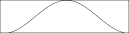
\includegraphics[scale=1]{gen19} 


 Diagram of the waveform generated by GEN19.


 \textbf{Example 1. A simple example of the GEN19 routine.}

\begin{lstlisting}
/* gen19.orc */
; Initialize the global variables.
sr = 44100
kr = 4410
ksmps = 10
nchnls = 1

; Instrument #1.
instr 1
  ; Create an index over the length of our entire note.
  kcps init 1/p3
  kndx phasor kcps

  ; Read Table #1 with our index.
  ifn = 1
  ixmode = 1
  kval table kndx, ifn, ixmode

  ; Generate a sine waveform, use our Table #1 value to 
  ; vary its frequency by 100 Hz from its base frequency.
  ibasefreq = 440
  kfreq = kval * 100
  a1 oscil 20000, ibasefreq + kfreq, 2
  out a1
endin
/* gen19.orc */
        
\end{lstlisting}
\begin{lstlisting}
/* gen19.sco */
; Table #1: a bell curve (using GEN19).
f 1 0 16384 -19 1 1 260 1
; Table #2, a sine wave.
f 2 0 16384 10 1

; Play Instrument #1 for 3 seconds.
i 1 0 3
e
/* gen19.sco */
        
\end{lstlisting}
\subsection*{See Also}


 \emph{GEN09}
 and \emph{GEN10}

\subsection*{Credits}


 Example written by Kevin Conder
%\hline 


\begin{comment}
\begin{tabular}{lcr}
Previous &Home &Next \\
GEN18 &Up &GEN20

\end{tabular}


\end{document}
\end{comment}

%\begin{comment}
\documentclass[10pt]{article}
\usepackage{fullpage, graphicx, url}
\setlength{\parskip}{1ex}
\setlength{\parindent}{0ex}
\title{GEN20}
\begin{document}


\begin{tabular}{ccc}
The Alternative Csound Reference Manual & & \\
Previous & &Next

\end{tabular}

%\hline 
\end{comment}
\section{GEN20}
GEN20�--� Generates functions of different windows. \subsection*{Description}


  This subroutine generates functions of different windows. These windows are usually used for spectrum analysis or for grain envelopes. 
\subsection*{Syntax}


 \textbf{f}
 \# time size 20 window max [opt]
\subsection*{Initialization}


 \emph{size}
 -- number of points in the table. Must be a power of 2 ( + 1). 


 \emph{window}
 -- Type of window to generate: 


 
\begin{itemize}
\item 

 1 = Hamming

\item 

 2 = Hanning

\item 

 3 = Bartlett ( triangle)

\item 

 4 = Blackman ( 3-term)

\item 

 5 = Blackman - Harris ( 4-term)

\item 

 6 = Gaussian

\item 

 7 = Kaiser

\item 

 8 = Rectangle

\item 

 9 = Sync


\end{itemize}


 \emph{max}
 -- For negative p4 this will be the absolute value at window peak point. If p4 is positive or p4 is negative and p6 is missing the table will be post-rescaled to a maximum value of 1. 


 \emph{opt}
 -- Optional argument required by the Kaiser window. 
\subsection*{Examples}


 


 
\begin{lstlisting}
\emph{f}
       1       0       1024    20      5
        
\end{lstlisting}


 
 This creates a function which contains a 4 - term Blackman - Harris window with maximum value of 1. 

 


 
\begin{lstlisting}
\emph{f}
       1       0       1024    -20     2       456
        
\end{lstlisting}


 
 This creates a function that contains a Hanning window with a maximum value of 456. 

 


 
\begin{lstlisting}
\emph{f}
       1       0       1024    -20     1
        
\end{lstlisting}


 
 This creates a function that contains a Hamming window with a maximum value of 1. 

 


 
\begin{lstlisting}
\emph{f}
       1       0       1024    20      7       1       2
        
\end{lstlisting}


 
 This creates a function that contains a Kaiser window with a maximum value of 1. The extra argument specifies how ``open'' the window is, for example a value of 0 results in a rectangular window and a value of 10 in a Hamming like window. 

  For diagrams, see \emph{Window Functions}

\subsection*{Credits}


 


 


\begin{tabular}{ccc}
Author: Paris Smaragdis &MIT, Cambridge &1995

\end{tabular}



 


 


 


\begin{tabular}{ccc}
Author: John ffitch &University of Bath/Codemist Ltd. &Bath, UK

\end{tabular}



 


 New in Csound version 3.2
%\hline 


\begin{comment}
\begin{tabular}{lcr}
Previous &Home &Next \\
GEN19 &Up &GEN21

\end{tabular}


\end{document}
\end{comment}

%\begin{comment}
\documentclass[10pt]{article}
\usepackage{fullpage, graphicx, url}
\setlength{\parskip}{1ex}
\setlength{\parindent}{0ex}
\title{GEN21}
\begin{document}


\begin{tabular}{ccc}
The Alternative Csound Reference Manual & & \\
Previous & &Next

\end{tabular}

%\hline 
\end{comment}
\section{GEN21}
GEN21�--� Generates tables of different random distributions. \subsection*{Description}


  This generates tables of different random distributions. (See also \emph{betarand}
, \emph{bexprnd}
, \emph{cauchy}
, \emph{exprand}
, \emph{gauss}
, \emph{linrand}
, \emph{pcauchy}
, \emph{poisson}
, \emph{trirand}
, \emph{unirand}
, and \emph{weibull}
) 
\subsection*{Syntax}


 \textbf{f}
 \# time size 21 type level [arg1 [arg2]]
\subsection*{Initialization}


 \emph{time}
 and \emph{size}
 are the usual GEN function arguments. \emph{level}
 defines the amplitude. Note that GEN21 is not self-normalizing as are most other GEN functions. \emph{type}
 defines the distribution to be used as follow: 


 
\begin{itemize}
\item 

 1 = Uniform (positive numbers only)

\item 

 2 = Linear (positive numbers only)

\item 

 3 = Triangular (positive and negative numbers)

\item 

 4 = Exponential (positive numbers only)

\item 

 5 = Biexponential (positive and negative numbers)

\item 

 6 = Gaussian (positive and negative numbers)

\item 

 7 = Cauchy (positive and negative numbers)

\item 

 8 = Positive Cauchy (positive numbers only)

\item 

 9 = Beta (positive numbers only)

\item 

 10 = Weibull (positive numbers only)

\item 

 11 = Poisson (positive numbers only)


\end{itemize}
 Of all these cases only 9 (Beta) and 10 (Weibull) need extra arguments. Beta needs two arguments and Weibull one. \subsection*{Examples}


 


 
\begin{lstlisting}
\emph{f}
1 0 1024 21 1       ; Uniform (white noise)
\emph{f}
1 0 1024 21 6       ; Gaussian
\emph{f}
1 0 1024 21 9 1 1 2 ; Beta (note that level precedes arguments)
\emph{f}
1 0 1024 21 10 1 2  ; Weibull
        
\end{lstlisting}


 
 All of the above additions were designed by the author between May and December 1994, under the supervision of Dr. Richard Boulanger. \subsection*{Credits}


 


 


\begin{tabular}{ccc}
Author: Paris Smaragdis &MIT, Cambridge &1995

\end{tabular}



 


 


 


\begin{tabular}{ccc}
Author: John ffitch &University of Bath/Codemist Ltd. &Bath, UK

\end{tabular}



 


 New in Csound version 3.2
%\hline 


\begin{comment}
\begin{tabular}{lcr}
Previous &Home &Next \\
GEN20 &Up &GEN22

\end{tabular}


\end{document}
\end{comment}

%\begin{comment}
\documentclass[10pt]{article}
\usepackage{fullpage, graphicx, url}
\setlength{\parskip}{1ex}
\setlength{\parindent}{0ex}
\title{GEN22}
\begin{document}


\begin{tabular}{ccc}
The Alternative Csound Reference Manual & & \\
Previous & &Next

\end{tabular}

%\hline 
\end{comment}
\section{GEN22}
GEN22�--� Deprecated. \subsection*{Description}


  Deprecated as of version 4.19. Use the \emph{GEN18}
 routine instead. 
%\hline 


\begin{comment}
\begin{tabular}{lcr}
Previous &Home &Next \\
GEN21 &Up &GEN23

\end{tabular}


\end{document}
\end{comment}

%\begin{comment}
\documentclass[10pt]{article}
\usepackage{fullpage, graphicx, url}
\setlength{\parskip}{1ex}
\setlength{\parindent}{0ex}
\title{GEN23}
\begin{document}


\begin{tabular}{ccc}
The Alternative Csound Reference Manual & & \\
Previous & &Next

\end{tabular}

%\hline 
\end{comment}
\section{GEN23}
GEN23�--� Reads numeric values from a text file. \subsection*{Description}


  This subroutine reads numeric values from an external ASCII file. 
\subsection*{Syntax}


 \textbf{f}
 \# time size -23 ``filename.txt''
\subsection*{Initialization}


 \emph{``filename.txt''}
 -- numeric values contained in ``filename.txt'' (which indicates the complete pathname of the character file to be read), can be separated by spaces, tabs, newline characters or commas. Also, words that contains non-numeric characters can be used as comments since they are ignored. 


 \emph{size}
 -- number of points in the table. Must be a power of 2 , power of 2 + 1, or zero. If \emph{size}
 = 0, table size is determined by the number of numeric values in \emph{filename.txt}
. (New in Csound version 3.57) 


 


\begin{tabular}{cc}
\textbf{Note}
 \\
� &

  All characters following ';' (comment) are ignored until next line (numbers too). 


\end{tabular}

\subsection*{Credits}


 


 


\begin{tabular}{ccc}
Author: Gabriel Maldonado &Italy &February, 1998

\end{tabular}



 


 New in Csound version 3.47
%\hline 


\begin{comment}
\begin{tabular}{lcr}
Previous &Home &Next \\
GEN22 &Up &GEN24

\end{tabular}


\end{document}
\end{comment}

%\begin{comment}
\documentclass[10pt]{article}
\usepackage{fullpage, graphicx, url}
\setlength{\parskip}{1ex}
\setlength{\parindent}{0ex}
\title{GEN24}
\begin{document}


\begin{tabular}{ccc}
The Alternative Csound Reference Manual & & \\
Previous & &Next

\end{tabular}

%\hline 
\end{comment}
\section{GEN24}
GEN24�--� Reads numeric values from another allocated function-table and rescales them. \subsection*{Description}


  This subroutine reads numeric values from another allocated function-table and rescales them according to the max and min values given by the user. 
\subsection*{Syntax}


 \textbf{f}
 \# time size -24 ftable min max
\subsection*{Initialization}


 \emph{\#, time, size}
 -- the usual GEN parameters. See f statement. 


 \emph{ftable}
 -- ftable must be an already allocated table with the same size as this function. 


 \emph{min, max}
 -- the rescaling range. 


 


\begin{tabular}{cc}
\textbf{Note}
 \\
� &

  This GEN is useful, for example, to eliminate the starting offset in exponential segments allowing a real starting from zero. 


\end{tabular}

\subsection*{Credits}


 Author: Gabriel Maldonado


 New in Csound version 4.16
%\hline 


\begin{comment}
\begin{tabular}{lcr}
Previous &Home &Next \\
GEN23 &Up &GEN25

\end{tabular}


\end{document}
\end{comment}

%\begin{comment}
\documentclass[10pt]{article}
\usepackage{fullpage, graphicx, url}
\setlength{\parskip}{1ex}
\setlength{\parindent}{0ex}
\title{GEN25}
\begin{document}


\begin{tabular}{ccc}
The Alternative Csound Reference Manual & & \\
Previous & &Next

\end{tabular}

%\hline 
\end{comment}
\section{GEN25}
GEN25�--� Construct functions from segments of exponential curves in breakpoint fashion. \subsection*{Description}


  These subroutines are used to construct functions from segments of exponential curves in breakpoint fashion. 
\subsection*{Syntax}


 \textbf{f}
 \# time size 25 x1 y1 x2 y2 x3 ...
\subsection*{Initialization}


 \emph{size }
 -- number of points in the table. Must be a power of 2 or power-of-2 plus 1 (see \emph{f statement}
). 


 \emph{x1, x2, x3,}
 etc. -- locations in table at which to attain the following y value. Must be in increasing order. If the last value is less than size, then the rest will be set to zero. Should not be negative but can be zero. 


 \emph{y1, y2, y3,}
, etc. -- Breakpoint values attained at the location specified by the preceding x value. These must be non-zero and must be alike in sign. 


 


\begin{tabular}{cc}
\textbf{Note}
 \\
� &

  If p4 is positive, functions are post-normalized (rescaled to a maximum absolute value of 1 after generation). A negative p4 will cause rescaling to be skipped. 


\end{tabular}

\subsection*{See Also}


 \emph{f statement}
, \emph{GEN27}

\subsection*{Credits}


 


 


\begin{tabular}{ccc}
Author: John ffitch &University of Bath/Codemist Ltd. &Bath, UK

\end{tabular}



 


 New in Csound version 3.49
%\hline 


\begin{comment}
\begin{tabular}{lcr}
Previous &Home &Next \\
GEN24 &Up &GEN27

\end{tabular}


\end{document}
\end{comment}

%\begin{comment}
\documentclass[10pt]{article}
\usepackage{fullpage, graphicx, url}
\setlength{\parskip}{1ex}
\setlength{\parindent}{0ex}
\title{GEN27}
\begin{document}


\begin{tabular}{ccc}
The Alternative Csound Reference Manual & & \\
Previous & &Next

\end{tabular}

%\hline 
\end{comment}
\section{GEN27}
GEN27�--� Construct functions from segments of straight lines in breakpoint fashion. \subsection*{Description}


  Construct functions from segments of straight lines in breakpoint fashion. 
\subsection*{Syntax}


 \textbf{f}
 \# time size 27 x1 y1 x2 y2 x3 ...
\subsection*{Initialization}


 \emph{size }
 -- number of points in the table. Must be a power of 2 or power-of-2 plus 1 (see \emph{f statement}
). 


 \emph{x1, x2, x3,}
 etc. -- locations in table at which to attain the following y value. Must be in increasing order. If the last value is less than size, then the rest will be set to zero. Should not be negative but can be zero. 


 \emph{y1, y2, y3,}
, etc. -- Breakpoint values attained at the location specified by the preceding x value. 


 


\begin{tabular}{cc}
\textbf{Note}
 \\
� &

  If p4 is positive, functions are post-normalized (rescaled to a maximum absolute value of 1 after generation). A negative p4 will cause rescaling to be skipped. 


\end{tabular}

\subsection*{Examples}


 


 
\begin{lstlisting}
\emph{f}
 1 0 257 27 0 0 100 1 200 -1 256 0
        
\end{lstlisting}


 
 This describes a function which begins at 0, rises to 1 at the 100th table location, falls to -1, by the 200th location, and returns to 0 by the end of the table. The interpolation is linear. \subsection*{See Also}


 \emph{f statement}
, \emph{GEN25}

\subsection*{Credits}


 


 


\begin{tabular}{ccc}
Author: John ffitch &University of Bath/Codemist Ltd. &Bath, UK

\end{tabular}



 


 New in Csound version 3.49
%\hline 


\begin{comment}
\begin{tabular}{lcr}
Previous &Home &Next \\
GEN25 &Up &GEN28

\end{tabular}


\end{document}
\end{comment}

%\begin{comment}
\documentclass[10pt]{article}
\usepackage{fullpage, graphicx, url}
\setlength{\parskip}{1ex}
\setlength{\parindent}{0ex}
\title{GEN28}
\begin{document}


\begin{tabular}{ccc}
The Alternative Csound Reference Manual & & \\
Previous & &Next

\end{tabular}

%\hline 
\end{comment}
\section{GEN28}
GEN28�--� Reads a text file which contains a time-tagged trajectory. \subsection*{Description}


  This function generator reads a text file which contains sets of three values representing the xy coordinates and a time-tag for when the signal should be placed at that location, allowing the user to define a time-tagged trajectory. The file format is in the form: 


 time1����X1������Y1\\ 
 time2����X2������Y2\\ 
 time3����X3������Y3\\ 
 ������


  The configuration of the xy coordinates in space places the signal in the following way: 


 
\begin{itemize}
\item 

 a1 is -1, 1

\item 

 a2 is 1, 1

\item 

 a3 is -1, -1

\item 

 a4 is 1, -1


\end{itemize}


  This assumes a loudspeaker set up as a1 is left front, a2 is right front, a3 is left back, a4 is right back. Values greater than 1 will result in sounds being attenuated as if in the distance. \emph{GEN28}
 creates values to 10 milliseconds of resolution. 
\subsection*{Syntax}


 \textbf{f}
 \# time size 28 ifilcod
\subsection*{Initialization}


 \emph{size}
 -- number of points in the table. Must be 0. \emph{GEN28}
 takes 0 as the size and automatically allocates memory. 


 \emph{ifilcod}
 -- character-string denoting the source soundfile name. A character-string (in double quotes, spaces permitted) gives the filename itself, optionally a full pathname. If not a full path, the named file is sought in the current directory. 
\subsection*{Examples}


 


 
\begin{lstlisting}
f1 0 0 28 "move"
        
\end{lstlisting}


 


  The file ``move'' should look like: 


 0�������-1�������1\\ 
 1��������1�������1\\ 
 2��������4�������4\\ 
 2.1�����-4������-4\\ 
 3��������10�����-10\\ 
 5�������-40������0\\ 
 ������
 Since \emph{GEN28}
 creates values to 10 milliseconds of resolution, there will be 500 values created by interpolating X1 to X2 to X3 and so on, and Y1 to Y2 to Y3 and so on, over the appropriate number of values that are stored in the function table. The sound will begin in the left front, over 1 second it will move to the right front, over another second it move further into the distance but still in the left front, then in just 1/10th of a second it moves to the left rear, a bit distant. Finally over the last .9 seconds the sound will move to the right rear, moderately distant, and it comes to rest between the two left channels (due west!), quite distant. \subsection*{Credits}


 


 


\begin{tabular}{ccc}
Author: Richard Karpen &Seattle, Wash &1998

\end{tabular}



 


 New in Csound version 3.48
%\hline 


\begin{comment}
\begin{tabular}{lcr}
Previous &Home &Next \\
GEN27 &Up &GEN30

\end{tabular}


\end{document}
\end{comment}

%\begin{comment}
\documentclass[10pt]{article}
\usepackage{fullpage, graphicx, url}
\setlength{\parskip}{1ex}
\setlength{\parindent}{0ex}
\title{GEN30}
\begin{document}


\begin{tabular}{ccc}
The Alternative Csound Reference Manual & & \\
Previous & &Next

\end{tabular}

%\hline 
\end{comment}
\section{GEN30}
GEN30�--� Generates harmonic partials by analyzing an existing table. \subsection*{Description}


  Extracts a range of harmonic partials from an existing waveform. 
\subsection*{Syntax}


 \textbf{f}
 \# time size 30 src minh maxh [ref\_sr] [interp]
\subsection*{Performance}


 \emph{src}
 -- source ftable 


 \emph{minh}
 -- lowest harmonic number 


 \emph{maxh}
 -- highest harmonic number 


 \emph{ref\_sr}
 (optional) -- maxh is scaled by (sr / ref\_sr). The default value of ref\_sr is sr. If \emph{ref\_sr}
 is zero or negative, it is now ignored. 


 \emph{interp}
 (optional) -- if non-zero, allows changing the amplitude of the lowest and highest harmonic partial depending on the fractional part of \emph{minh}
 and \emph{maxh}
. For example, if \emph{maxh}
 is 11.3 then the 12th harmonic partial is added with 0.3 amplitude. This parameter is zero by default. 


 \emph{GEN30}
 does not support tables with an extended guard point (ie. table size = power of two + 1). Although such tables will work both for input and output, when reading source table(s), the guard point is ignored, and when writing the output table, guard point is simply copied from the first sample (table index = 0). 


  The reason of this limitation is that \emph{GEN30}
 uses FFT, which requires power of two table size. \emph{GEN32}
 allows using linear interpolation for resampling and phase shifting, which makes it possible to use any table size (however, for partials calculated with FFT, the power of two limitation still exists). 
\subsection*{Credits}


 Author: Istvan Varga


 New in version 4.16
%\hline 


\begin{comment}
\begin{tabular}{lcr}
Previous &Home &Next \\
GEN28 &Up &GEN31

\end{tabular}


\end{document}
\end{comment}

%\begin{comment}
\documentclass[10pt]{article}
\usepackage{fullpage, graphicx, url}
\setlength{\parskip}{1ex}
\setlength{\parindent}{0ex}
\title{GEN31}
\begin{document}


\begin{tabular}{ccc}
The Alternative Csound Reference Manual & & \\
Previous & &Next

\end{tabular}

%\hline 
\end{comment}
\section{GEN31}
GEN31�--� Mixes any waveform specified in an existing table. \subsection*{Description}


  This routine is similar to GEN09, but allows mixing any waveform specified in an existing table. 
\subsection*{Syntax}


 \textbf{f}
 \# time size 31 src pna stra phsa pnb strb phsb ...
\subsection*{Performance}


 \emph{src}
 -- source table number 


 \emph{pna, pnb, ...}
 -- partial number, must be a positive integer 


 \emph{stra, strb, ...}
 -- amplitude scale 


 \emph{phsa, phsb, ...}
 -- start phase (0 to 1) 


 \emph{GEN31}
 does not support tables with an extended guard point (ie. table size = power of two + 1). Although such tables will work both for input and output, when reading source table(s), the guard point is ignored, and when writing the output table, guard point is simply copied from the first sample (table index = 0). 


  The reason of this limitation is that \emph{GEN31}
 uses FFT, which requires power of two table size. \emph{GEN32}
 allows using linear interpolation for resampling and phase shifting, which makes it possible to use any table size (however, for partials calculated with FFT, the power of two limitation still exists). 
\subsection*{Credits}


 Author: Istvan Varga


 New in version 4.15
%\hline 


\begin{comment}
\begin{tabular}{lcr}
Previous &Home &Next \\
GEN30 &Up &GEN32

\end{tabular}


\end{document}
\end{comment}

%\begin{comment}
\documentclass[10pt]{article}
\usepackage{fullpage, graphicx, url}
\setlength{\parskip}{1ex}
\setlength{\parindent}{0ex}
\title{GEN32}
\begin{document}


\begin{tabular}{ccc}
The Alternative Csound Reference Manual & & \\
Previous & &Next

\end{tabular}

%\hline 
\end{comment}
\section{GEN32}
GEN32�--� Mixes any waveform, resampled with either FFT or linear interpolation. \subsection*{Description}


  This routine is similar to \emph{GEN31}
, but allows specifying source ftable for each partial. Tables can be resampled either with FFT, or linear interpolation. 
\subsection*{Syntax}


 \textbf{f}
 \# time size 32 srca pna stra phsa srcb pnb strb phsb ...
\subsection*{Performance}


 \emph{srca, srcb}
 -- source table number. A negative value can be used to read the table with linear interpolation (by default, the source waveform is transposed and phase shifted using FFT); this is less accurate, but faster, and allows non-integer and negative partial numbers. 


 \emph{pna, pnb, ...}
 -- partial number, must be a positive integer if source table number is positive (i.e. resample with FFT). 


 \emph{stra, strb, ...}
 -- amplitude scale 


 \emph{phsa, phsb, ...}
 -- start phase (0 to 1) 
\subsection*{Examples}


 


 
\begin{lstlisting}
itmp    ftgen 1, 0, 16384, 7, 1, 16384, -1      ; sawtooth
itmp    ftgen 2, 0, 8192, 10, 1                 ; sine
; mix tables
itmp    ftgen 5, 0, 4096, -32, -2, 1.5, 1.0, 0.25, 1, 2, 0.5, 0,        \
                                1, 3, -0.25, 0.5
; window
itmp    ftgen 6, 0, 16384, 20, 3, 1
; generate band-limited waveforms
inote   =  0
loop0:
icps    =  440 * exp(log(2) * (inote - 69) / 12)        ; one table for
inumh   =  sr / (2 * icps)                              ; each MIDI note number
ift     =  int(inote + 256.5)
itmp    ftgen ift, 0, 4096, -30, 5, 1, inumh
inote   =  inote + 1
        if (inote < 127.5) igoto loop0

        instr 1

kcps    expon 20, p3, 16000
kft     =  int(256.5 + 69 + 12 * log(kcps / 440) / log(2))
kft     =  (kft > 383 ? 383 : kft)

a1      phasor kcps
a1      tableikt a1, kft, 1, 0, 1

        out a1 * 10000

        endin
        instr 2

kcps    expon 20, p3, 16000
kft     =  int(256.5 + 69 + 12 * log(kcps / 440) / log(2))
kft     =  (kft > 383 ? 383 : kft)

kgdur   limit 10 / kcps, 0.1, 1
a1      grain2 kcps, 0.02, kgdur, 30, kft, 6, -0.5

        out a1 * 2000

        endin

----------
score:
----------

t 0 60
i 1 0 10
i 2 12 10
e
        
\end{lstlisting}


 
\subsection*{Credits}


 Author: Rasmus Ekman


 Programmer: Istvan Varga


 New in version 4.17
%\hline 


\begin{comment}
\begin{tabular}{lcr}
Previous &Home &Next \\
GEN31 &Up &GEN33

\end{tabular}


\end{document}
\end{comment}

%\begin{comment}
\documentclass[10pt]{article}
\usepackage{fullpage, graphicx, url}
\setlength{\parskip}{1ex}
\setlength{\parindent}{0ex}
\title{GEN33}
\begin{document}


\begin{tabular}{ccc}
The Alternative Csound Reference Manual & & \\
Previous & &Next

\end{tabular}

%\hline 
\end{comment}
\section{GEN33}
GEN33�--� Generate composite waveforms by mixing simple sinusoids. \subsection*{Description}


  These routines generate composite waveforms by mixing simple sinusoids, similarly to \emph{GEN09}
, but the parameters of the partials are specified in an already existing table, which makes it possible to calculate any number of partials in the orchestra. 


  The difference between \emph{GEN33}
 and \emph{GEN34}
 is that \emph{GEN33}
 uses inverse FFT to generate output, while \emph{GEN34}
 is based on the algorithm used in oscils opcode. \emph{GEN33}
 allows integer partials only, and does not support power of two plus 1 table size, but may be significantly faster with a large number of partials. On the other hand, with \emph{GEN34}
, it is possible to use non-integer partial numbers and extended guard point, and this routine may be faster if there is only a small number of partials (note that \emph{GEN34}
 is also several times faster than \emph{GEN09}
, although the latter may be more accurate). 
\subsection*{Syntax}


 \textbf{f}
 \# time size 33 src nh scl [fmode]
\subsection*{Initialization}


 \emph{size}
 -- number of points in the table. Must be power of two and at least 4. 


 \emph{src}
 -- source table number. This table contains the parameters of each partial in the following format: 


 stra,�pna,�phsa,�strb,�pnb,�phsb,�...\\ 
 �����
 the parameters are: 

 
\begin{itemize}
\item 

 stra, strb, etc.: relative strength of partials. The actual amplitude depends on the value of scl, or normalization (if enabled).

\item 

 pna, pnb, etc.: partial number, or frequency, depending on fmode (see below); zero and negative values are allowed, however, if the absolute value of the partial number exceeds (size / 2), the partial will not be rendered. With \emph{GEN33}
, partial number is rounded to the nearest integer.

\item 

 phsa, phsb, etc.: initial phase, in the range 0 to 1.


\end{itemize}
 Table length (not including the guard point) should be at least 3 * nh. If the table is too short, the number of partials (nh) is reduced to (table length) / 3, rounded towards zero. 

 \emph{nh}
 -- number of partials. Zero or negative values are allowed, and result in an empty table (silence). The actual number may be reduced if the source table (src) is too short, or some partials have too high frequency. 


 \emph{scl}
 -- amplitude scale. 


 \emph{fmode}
 (optional, default = 0) -- a non-zero value can be used to set frequency in Hz instead of partial numbers in the source table. The sample rate is assumed to be fmode if it is positive, or -(sr * fmode) if any negative value is specified. 
\subsection*{Examples}


 


 
\begin{lstlisting}
; partials 1, 4, 7, 10, 13, 16, etc. with base frequency of 400 Hz

ibsfrq  =  400
; estimate number of partials
inumh   =  int(1.5 + sr * 0.5 / (3 * ibsfrq))
; source table length
isrcln  =  int(0.5 + exp(log(2) * int(1.01 + log(inumh * 3) / log(2))))
; create empty source table
itmp    ftgen 1, 0, isrcln, -2, 0
ifpos   =  0
ifrq    =  ibsfrq
inumh   =  0
l1:
        tableiw ibsfrq / ifrq, ifpos, 1         ; amplitude
        tableiw ifrq, ifpos + 1, 1              ; frequency
        tableiw 0, ifpos + 2, 1                 ; phase
ifpos   =  ifpos + 3
ifrq    =  ifrq + ibsfrq * 3
inumh   =  inumh + 1
        if (ifrq < (sr * 0.5)) igoto l1

; store output in ftable 2 (size = 262144)

itmp    ftgen 2, 0, 262144, -34, 1, inumh, 1, -1
        
\end{lstlisting}


 
\subsection*{See Also}


 \emph{GEN09}
, \emph{GEN34}

\subsection*{Credits}


 


 


\begin{tabular}{cc}
Programmer: Istvan Varga &March 2002

\end{tabular}



 


 New in version 4.19
%\hline 


\begin{comment}
\begin{tabular}{lcr}
Previous &Home &Next \\
GEN32 &Up &GEN34

\end{tabular}


\end{document}
\end{comment}

%\begin{comment}
\documentclass[10pt]{article}
\usepackage{fullpage, graphicx, url}
\setlength{\parskip}{1ex}
\setlength{\parindent}{0ex}
\title{GEN34}
\begin{document}


\begin{tabular}{ccc}
The Alternative Csound Reference Manual & & \\
Previous & &Next

\end{tabular}

%\hline 
\end{comment}
\section{GEN34}
GEN34�--� Generate composite waveforms by mixing simple sinusoids. \subsection*{Description}


  These routines generate composite waveforms by mixing simple sinusoids, similarly to \emph{GEN09}
, but the parameters of the partials are specified in an already existing table, which makes it possible to calculate any number of partials in the orchestra. 


  The difference between \emph{GEN33}
 and \emph{GEN34}
 is that \emph{GEN33}
 uses inverse FFT to generate output, while \emph{GEN34}
 is based on the algorithm used in oscils opcode. \emph{GEN33}
 allows integer partials only, and does not support power of two plus 1 table size, but may be significantly faster with a large number of partials. On the other hand, with \emph{GEN34}
, it is possible to use non-integer partial numbers and extended guard point, and this routine may be faster if there is only a small number of partials (note that \emph{GEN34}
 is also several times faster than \emph{GEN09}
, although the latter may be more accurate). 
\subsection*{Syntax}


 \textbf{f}
 \# time size 34 src nh scl [fmode]
\subsection*{Initialization}


 \emph{size}
 -- number of points in the table. Must be power of two or a power of two plus 1. 


 \emph{src}
 -- source table number. This table contains the parameters of each partial in the following format: 


 stra,�pna,�phsa,�strb,�pnb,�phsb,�...\\ 
 �����
 the parameters are: 

 
\begin{itemize}
\item 

 stra, strb, etc.: relative strength of partials. The actual amplitude depends on the value of scl, or normalization (if enabled).

\item 

 pna, pnb, etc.: partial number, or frequency, depending on fmode (see below); zero and negative values are allowed, however, if the absolute value of the partial number exceeds (size / 2), the partial will not be rendered.

\item 

 phsa, phsb, etc.: initial phase, in the range 0 to 1.


\end{itemize}
 Table length (not including the guard point) should be at least 3 * nh. If the table is too short, the number of partials (nh) is reduced to (table length) / 3, rounded towards zero. 

 \emph{nh}
 -- number of partials. Zero or negative values are allowed, and result in an empty table (silence). The actual number may be reduced if the source table (src) is too short, or some partials have too high frequency. 


 \emph{scl}
 -- amplitude scale. 


 \emph{fmode}
 (optional, default = 0) -- a non-zero value can be used to set frequency in Hz instead of partial numbers in the source table. The sample rate is assumed to be fmode if it is positive, or -(sr * fmode) if any negative value is specified. 
\subsection*{Examples}


 


 
\begin{lstlisting}
; partials 1, 4, 7, 10, 13, 16, etc. with base frequency of 400 Hz

ibsfrq  =  400
; estimate number of partials
inumh   =  int(1.5 + sr * 0.5 / (3 * ibsfrq))
; source table length
isrcln  =  int(0.5 + exp(log(2) * int(1.01 + log(inumh * 3) / log(2))))
; create empty source table
itmp    ftgen 1, 0, isrcln, -2, 0
ifpos   =  0
ifrq    =  ibsfrq
inumh   =  0
l1:
        tableiw ibsfrq / ifrq, ifpos, 1         ; amplitude
        tableiw ifrq, ifpos + 1, 1              ; frequency
        tableiw 0, ifpos + 2, 1                 ; phase
ifpos   =  ifpos + 3
ifrq    =  ifrq + ibsfrq * 3
inumh   =  inumh + 1
        if (ifrq < (sr * 0.5)) igoto l1

; store output in ftable 2 (size = 262144)

itmp    ftgen 2, 0, 262144, -34, 1, inumh, 1, -1
        
\end{lstlisting}


 
\subsection*{See Also}


 \emph{GEN09}
, \emph{GEN33}

\subsection*{Credits}


 


 


\begin{tabular}{cc}
Programmer: Istvan Varga &March 2002

\end{tabular}



 


 New in version 4.19
%\hline 


\begin{comment}
\begin{tabular}{lcr}
Previous &Home &Next \\
GEN33 &Up &GEN40

\end{tabular}


\end{document}
\end{comment}

%\begin{comment}
\documentclass[10pt]{article}
\usepackage{fullpage, graphicx, url}
\setlength{\parskip}{1ex}
\setlength{\parindent}{0ex}
\title{GEN40}
\begin{document}


\begin{tabular}{ccc}
The Alternative Csound Reference Manual & & \\
Previous & &Next

\end{tabular}

%\hline 
\end{comment}
\section{GEN40}
GEN40�--� Generates a random distribution using a distribution histogram. \subsection*{Description}


  Generates a continuous random distribution function starting from the shape of a user-defined distribution histogram. 
\subsection*{Syntax}


 \textbf{f}
 \# time size -40 shapetab
\subsection*{Performance}


  The shape of histogram must be stored in a previously defined table, in fact shapetab argument must be filled with the number of such table. 


  Histogram shape can be generated with any other GEN routines. Since no interpolation is used when GEN40 processes the translation, it is suggested that the size of the table containing the histogram shape to be reasonably big, in order to obtain more precision (however after the processing the shaping-table can be destroyed in order to re-gain memory). 


  This subroutine is designed to be used together with cuserrnd opcode (see cuserrnd for more information). 
\subsection*{Credits}


 Author: Gabriel Maldonado
%\hline 


\begin{comment}
\begin{tabular}{lcr}
Previous &Home &Next \\
GEN34 &Up &GEN41

\end{tabular}


\end{document}
\end{comment}

%\begin{comment}
\documentclass[10pt]{article}
\usepackage{fullpage, graphicx, url}
\setlength{\parskip}{1ex}
\setlength{\parindent}{0ex}
\title{GEN41}
\begin{document}


\begin{tabular}{ccc}
The Alternative Csound Reference Manual & & \\
Previous & &Next

\end{tabular}

%\hline 
\end{comment}
\section{GEN41}
GEN41�--� Generates a random list of numerical pairs. \subsection*{Description}


  Generates a discrete random distribution function by giving a list of numerical pairs. 
\subsection*{Syntax}


 \textbf{f}
 \# time size -41 value1 prob1 value2 prob2 value3 prob3 ... valueN probN 
\subsection*{Performance}


  The first number of each pair is a value, and the second is the probability of that value to be chosen by a random algorithm. Even if any number can be assigned to the probability element of each pair, it is suggested to give it a percent value, in order to make it clearer for the user. 


  This subroutine is designed to be used together with duserrnd and \emph{urd}
 opcodes (see duserrnd for more information). 
\subsection*{Credits}


 Author: Gabriel Maldonado
%\hline 


\begin{comment}
\begin{tabular}{lcr}
Previous &Home &Next \\
GEN40 &Up &GEN42

\end{tabular}


\end{document}
\end{comment}

%\begin{comment}
\documentclass[10pt]{article}
\usepackage{fullpage, graphicx, url}
\setlength{\parskip}{1ex}
\setlength{\parindent}{0ex}
\title{GEN42}
\begin{document}


\begin{tabular}{ccc}
The Alternative Csound Reference Manual & & \\
Previous & &Next

\end{tabular}

%\hline 
\end{comment}
\section{GEN42}
GEN42�--� Generates a random distribution of discrete ranges of values. \subsection*{Description}


  Generates a random distribution function of discrete ranges of values by giving a list of groups of three numbers. 
\subsection*{Syntax}


 \textbf{f}
 \# time size -42 min1 max1 prob1 min2 max2 prob2 min3 max3 prob3 ... minN maxN probN
\subsection*{Performance}


  The first number of each group is a the minimum value of the first range, the second is the maximum value and the third is the probability of that an element belonging to that range of values can be chosen by a random algorithm. Even if any number can be assigned to the probability element of each group, it is suggested to give it a percent value, in order to make it clearer to the user. 


  This subroutine is designed to be used together with duserrnd and \emph{urd}
 opcodes (see duserrnd for more information). Since both duserrnd and urd do not use any interpolation, it is suggested to give a size reasonably big. 
\subsection*{Credits}


 Author: Gabriel Maldonado
%\hline 


\begin{comment}
\begin{tabular}{lcr}
Previous &Home &Next \\
GEN41 &Up &The Utility Programs

\end{tabular}


\end{document}
\end{comment}

%\begin{comment}
\documentclass[10pt]{article}
\usepackage{fullpage, graphicx, url}
\setlength{\parskip}{1ex}
\setlength{\parindent}{0ex}
\title{Index}
\begin{document}


\begin{tabular}{ccc}
The Alternative Csound Reference Manual & & \\
Previous & &�

\end{tabular}

%\hline 
\end{comment}
\section{Index}
\section{Symbols}
\begin{description}
\item[!=, !=]\item[\#define, \#define]\begin{description}
\item[orchestra, \#define]\begin{description}

\end{description}

\item[score, Description]\begin{description}

\end{description}


\end{description}

\item[\#include ]\begin{description}
\item[orchestra, \#include]\begin{description}

\end{description}

\item[score, Performance]\begin{description}

\end{description}


\end{description}

\item[\#undef, \#undef]\begin{description}
\item[orchestra, \#undef]\begin{description}

\end{description}

\item[score, Description]\begin{description}

\end{description}


\end{description}

\item[\$NAME, \$NAME]\begin{description}
\item[orchestra, \$NAME]\begin{description}

\end{description}

\item[score, Description]\begin{description}

\end{description}


\end{description}

\item[\%, \%]\item[\&\#732;, Ramping]\item[\&\&, \&\&]\item[$>$, $>$]\item[$>$=, $>$=]\item[$<$, $<$]\item[$<$=, $<$=]\item[$<$CsInstruments$>$, Description]\item[$<$CsMidifileB$>$, Description]\item[$<$CsOptions$>$, Description]\item[$<$CsoundSynthesizer$>$, Description]\item[$<$CsSampleB$>$, Description]\item[$<$CsScore$>$, Description]\item[$<$CsVersion$>$, Description]\item[(, Ramping]\item[), Ramping]\item[*, *]\item[+, +]\item[-, -]\item[--aiff, Command-line Flags]\item[--analysis-directory, Command-line Flags]\item[--asciidisplay, Command-line Flags]\item[--control-rate, Command-line Flags]\item[--cscore, Command-line Flags]\item[--defer-gen1, Command-line Flags]\item[--dither, Command-line Flags]\item[--extract-score, Command-line Flags]\item[--format=24bit, Command-line Flags]\item[--format=alaw, Command-line Flags]\item[--format=float, Command-line Flags]\item[--format=long, Command-line Flags]\item[--format=rescale, Command-line Flags]\item[--format=schar, Command-line Flags]\item[--format=short, Command-line Flags]\item[--format=uchar, Command-line Flags]\item[--format=ulaw, Command-line Flags]\item[--graphs, Command-line Flags]\item[--hardwarebufsamps, Command-line Flags]\item[--heartbeat, Command-line Flags]\item[--help, Command-line Flags]\item[--i-only, Command-line Flags]\item[--input, Command-line Flags]\item[--iobugsamps, Command-line Flags]\item[--ircam, Command-line Flags]\item[--keep-sorted-score, Command-line Flags]\item[--list-opcodesNUM, Command-line Flags]\item[--logfile, Command-line Flags]\item[--messagelevel, Command-line Flags]\item[--midi-device, Command-line Flags]\item[--midifile, Command-line Flags]\item[--nodisplays, Command-line Flags]\item[--noheader, Command-line Flags]\item[--nopeaks, Command-line Flags]\item[--nosound, Command-line Flags]\item[--notify, Command-line Flags]\item[--output, Command-line Flags]\item[--playonend, Command-line Flags]\item[--pollrate, Command-line Flags]\item[--postscriptdisplay, Command-line Flags]\item[--profile-rate, Command-line Flags]\item[--progress-rate, Command-line Flags]\item[--rewrite, Command-line Flags]\item[--sample-directory, Command-line Flags]\item[--sample-rate, Command-line Flags]\item[--save-midi, Command-line Flags]\item[--sched, Command-line Flags]\item[--score-in, Command-line Flags]\item[--screen-buffer, Command-line Flags]\item[--sound-directory, Command-line Flags]\item[--tempo=NUM, Command-line Flags]\item[--terminate-on-midi, Command-line Flags]\item[--utility, Command-line Flags]\item[--verbose, Command-line Flags]\item[--volume, Command-line Flags]\item[--wave, Command-line Flags]\item[-3, Command-line Flags]\item[-8, Command-line Flags]\item[-@, Command-line Flags]\item[-A, Command-line Flags]\item[-B, Command-line Flags]\item[-C, Command-line Flags]\item[-D, Command-line Flags]\item[-E, Command-line Flags]\item[-F, Command-line Flags]\item[-G, Command-line Flags]\item[-H, Command-line Flags]\item[-I, Command-line Flags]\item[-J, Command-line Flags]\item[-K, Command-line Flags]\item[-L, Command-line Flags]\item[-M, Command-line Flags]\item[-N, Command-line Flags]\item[-O, Command-line Flags]\item[-P, Command-line Flags]\item[-Q, Command-line Flags]\item[-R, Command-line Flags]\item[-s, Command-line Flags]\item[-T, Command-line Flags]\item[-t0, Command-line Flags]\item[-U, Command-line Flags]\item[-V, Command-line Flags]\item[-W, Command-line Flags]\item[-X, Command-line Flags]\item[-Y, Command-line Flags]\item[-Z, Command-line Flags]\item[.csd, Description]\item[.csoundrc, Description]\item[/, /]\item[0dbfs, 0dbfs]\item[:, !=, $>$, $>$=, $<$, $<$=, ==]\item[=, =]\item[==, ==]\item[?, !=, $>$, $>$=, $<$, $<$=, ==]\item[@, Evaluation of Expressions]\item[@@, Evaluation of Expressions]\item[\^{}, \^{}]\item[\{, Ramping]\item[||, ||]\item[\}, Ramping]
\end{description}
\section{A}
\begin{description}
\item[a, a]\item[a statement, a Statement (or Advance Statement)]\item[abetarand, abetarand]\item[abexprnd, abexprnd]\item[abs, abs]\item[acauchy, acauchy]\item[active, active]\item[adsr, adsr]\item[adsyn, adsyn]\item[adsynt, adsynt]\item[advance statement, a Statement (or Advance Statement)]\item[aexprand, aexprand]\item[aftouch, aftouch]\item[agauss, agauss]\item[agogobel, agogobel]\item[alinrand, alinrand]\item[alpass, alpass]\item[ampdb, ampdb]\item[ampdbfs, ampdbfs]\item[ampmidi, ampmidi]\item[apcauchy, apcauchy]\item[apoisson, apoisson]\item[apow, apow]\item[areson, areson]\item[aresonk, aresonk]\item[atone, atone]\item[atonek, atonek]\item[atonex, atonex]\item[atrirand, atrirand]\item[aunirand, aunirand]\item[aweibull, aweibull]
\end{description}
\section{B}
\begin{description}
\item[b statement, b Statement]\item[babo, babo]\item[balance, balance]\item[bamboo, bamboo]\item[bbcutm, bbcutm]\item[bbcuts, bbcuts]\item[betarand, betarand]\item[bexprnd, bexprnd]\item[biquad, biquad]\item[biquada, biquada]\item[birnd, birnd]\item[bqrez, bqrez]\item[bug reports ]\begin{description}
\item[code, Bug Reports]\begin{description}

\end{description}


\end{description}

\item[butbp, butbp]\item[butbr, butbr]\item[buthp, buthp]\item[butlp, butlp]\item[butterbp, butterbp]\item[butterbr, butterbr]\item[butterhp, butterhp]\item[butterlp, butterlp]\item[button, button]\item[buzz, buzz]
\end{description}
\section{C}
\begin{description}
\item[cabasa, cabasa]\item[cauchy, cauchy]\item[cent, cent]\item[cggoto, cggoto]\item[chanctrl, chanctrl]\item[checkbox, checkbox]\item[cigoto, cigoto]\item[ckgoto, ckgoto]\item[clear, clear]\item[clfilt, clfilt]\item[clip, clip]\item[clock, clock]\item[clockoff, clockoff]\item[clockon, clockon]\item[cngoto, cngoto]\item[comb, comb]\item[conditional expressions, !=, $>$, $>$=, $<$, $<$=, ==]\item[control, control]\item[convle, convle]\item[convolve, convolve]\item[cos, cos]\item[cosh, cosh]\item[cosinv, cosinv]\item[cps2pch, cps2pch]\item[cpsmidi, cpsmidi]\item[cpsmidib, cpsmidib]\item[cpsoct, cpsoct]\item[cpspch, cpspch]\item[cpstmid, cpstmid]\item[cpstun, cpstun]\item[cpstuni, cpstuni]\item[cpsxpch, cpsxpch]\item[cpuprc, cpuprc]\item[cross2, cross2]\item[crunch, crunch]\item[Cscore, Cscore]\item[CSSTRNGS, Directories and Files]\item[ctrl14, ctrl14]\item[ctrl21, ctrl21]\item[ctrl7, ctrl7]\item[ctrlinit, ctrlinit]\item[cuserrnd, cuserrnd]\item[cvanal, cvanal]
\end{description}
\section{D}
\begin{description}
\item[dam, dam]\item[db, db]\item[dbamp, dbamp]\item[dbfsamp, dbfsamp]\item[dcblock, dcblock]\item[dconv, dconv]\item[delay, delay]\item[delay1, delay1]\item[delayr, delayr]\item[delayw, delayw]\item[deltap, deltap]\item[deltape, deltap3]\item[deltapi, deltapi]\item[deltapn, deltapn]\item[deltapx, deltapx]\item[deltapxw, deltapxw]\item[diff, diff]\item[diskin, diskin]\item[dispfft, dispfft]\item[display, display]\item[distort1, distort1]\item[divz, divz]\item[dnoise, dnoise]\item[downsamp, downsamp]\item[dripwater, dripwater]\item[dumpk, dumpk]\item[dumpk2, dumpk2]\item[dumpk3, dumpk3]\item[dumpk4, dumpk4]\item[duserrnd, duserrnd]
\end{description}
\section{E}
\begin{description}
\item[e statement, e Statement]\item[else, else]\item[elseif, elseif]\item[endif, endif]\item[endin, endin]\item[endop, endop]\item[envlpx, envlpx]\item[envlpxr, envlpxr]\item[event, event]\item[exp, exp]\item[expon, expon]\item[exprand, exprand]\item[expseg, expseg]\item[expsega, expsega]\item[expsegr, expsegr]\item[extract, The Extract Feature]
\end{description}
\section{F}
\begin{description}
\item[f statement, f Statement (or Function Table Statement)]\item[filelen, filelen]\item[filenchnls, filenchnls]\item[filepeak, filepeak]\item[filesr, filesr]\item[filter2, filter2]\item[fin, fin]\item[fini, fini]\item[fink, fink]\item[fiopen, fiopen]\item[flags, Description]\item[flanger, flanger]\item[flashtxt, flashtxt]\item[FLbox, FLbox]\item[FLbutBank, FLbutBank]\item[FLbutton, FLbutton]\item[FLcolor, FLcolor]\item[FLcolor2, FLcolor2]\item[FLcount, FLcount]\item[FLgetsnap, FLgetsnap]\item[FLgroup, FLgroup]\item[FLgroupEnd, FLgroupEnd]\item[FLhide, FLhide]\item[FLjoy, FLjoy]\item[FLkeyb, FLkeyb]\item[FLknob, FLknob]\item[FLlabel, FLlabel]\item[FLloadsnap, FLloadsnap]\item[FLpack, FLpack]\item[FLpackEnd, FLpackEnd]\item[FLpanel, FLpanel]\item[FLpanelEnd, FLpanelEnd]\item[FLprintk, FLprintk]\item[FLprintk2, FLprintk2]\item[FLroller, FLroller]\item[FLrun, FLrun]\item[FLsavesnap, FLsavesnap]\item[FLscroll, FLscroll]\item[FLscrollEnd, FLscrollEnd]\item[FLsetAlign, FLsetAlign]\item[FLsetBox, FLsetBox]\item[FLsetColor, FLsetColor]\item[FLsetColor2, FLsetColor2]\item[FLsetFont, FLsetFont]\item[FLsetPosition, FLsetPosition]\item[FLsetSize, FLsetSize]\item[FLsetsnap, FLsetsnap]\item[FLsetText, FLsetText]\item[FLsetTextColor, FLsetTextColor]\item[FLsetTextSize, FLsetTextSize]\item[FLsetTextType, FLsetTextType]\item[FLsetVal, FLsetVal]\item[FLsetVal\_i, FLsetVal\_i]\item[FLshow, FLshow]\item[FLslidBnk, FLslidBnk]\item[FLslider, FLslider]\item[FLtabs, FLtabs]\item[FLtabsEnd, FLtabsEnd]\item[FLtext, FLtext]\item[FLupdate, FLupdate]\item[FLvalue, FLvalue]\item[fmb3, fmb3]\item[fmbell, fmbell]\item[fmmetal, fmmetal]\item[fmpercfl, fmpercfl]\item[fmrhode, fmrhode]\item[fmvoice, fmvoice]\item[fmwurlie, fmwurlie]\item[fof, fof]\item[fof2, fof2]\item[fog, fog]\item[fold, fold]\item[follow, follow]\item[follow2, follow2]\item[foscil, foscil]\item[foscili, foscili]\item[fout, fout]\item[fouti, fouti]\item[foutir, foutir]\item[foutk, foutk]\item[fprintks, fprintks]\item[fprints, fprints]\item[frac, frac]\item[ftchnls, ftchnls]\item[ftgen, ftgen]\item[ftlen, ftlen]\item[ftload, ftload]\item[ftloadk, ftloadk]\item[ftlptim, ftlptim]\item[ftmorf, ftmorf]\item[ftsave, ftsave]\item[ftsavek, ftsavek]\item[ftsr, ftsr]\item[function table statement, f Statement (or Function Table Statement)]
\end{description}
\section{G}
\begin{description}
\item[gain, gain]\item[gauss, gauss]\item[gbuzz, gbuzz]\item[GEN01, GEN01]\item[GEN02, GEN02]\item[GEN03, GEN03]\item[GEN04, GEN04]\item[GEN05, GEN05]\item[GEN06, GEN06]\item[GEN07, GEN07]\item[GEN08, GEN08]\item[GEN09, GEN09]\item[GEN10, GEN10]\item[GEN11, GEN11]\item[GEN12, GEN12]\item[GEN13, GEN13]\item[GEN14, GEN14]\item[GEN15, GEN15]\item[GEN16, GEN16]\item[GEN17, GEN17]\item[GEN18, GEN18]\item[GEN19, GEN19]\item[GEN20, GEN20]\item[GEN21, GEN21]\item[GEN22, GEN22]\item[GEN23, GEN23]\item[GEN24, GEN24]\item[GEN25, GEN25]\item[GEN27, GEN27]\item[GEN28, GEN28]\item[GEN30, GEN30]\item[GEN31, GEN31]\item[GEN32, GEN32]\item[GEN33, GEN33]\item[GEN34, GEN34]\item[GEN40, GEN40]\item[GEN41, GEN41]\item[GEN42, GEN42]\item[gogobel, gogobel]\item[goto, goto]\item[grain, grain]\item[grain2, grain2]\item[grain3, grain3]\item[granule, granule]\item[guiro, guiro]
\end{description}
\section{H}
\begin{description}
\item[harmon, harmon]\item[hetro, hetro]\item[hilbert, hilbert]\item[hrtfer, hrtfer]\item[hsboscil, hsboscil]
\end{description}
\section{I}
\begin{description}
\item[i, i]\item[i statement, i Statement (Instrument or Note Statement)]\item[ibetarand, ibetarand]\item[ibexprnd, ibexprnd]\item[icauchy, icauchy]\item[ictrl14, ictrl14]\item[ictrl21, ictrl21]\item[ictrl7, ictrl7]\item[iexprand, iexprand]\item[if, if]\item[igauss, igauss]\item[igoto, igoto]\item[ihold, ihold]\item[ilinrand, ilinrand]\item[imidic14, imidic14]\item[imidic21, imidic21]\item[imidic7, imidic7]\item[in, in]\item[in32, in32]\item[INCDIR, Directories and Files]\item[inch, inch]\item[inh, inh]\item[init, init]\item[initc14, initc14]\item[initc21, initc21]\item[initc7, initc7]\item[ink, ink]\item[ino, ino]\item[inq, inq]\item[ins, ins]\item[instimek, instimek]\item[instimes, instimes]\item[instr, instr]\item[instrument statement, i Statement (Instrument or Note Statement)]\item[int, int]\item[integ, integ]\item[interp, interp]\item[invalue, invalue]\item[inx, inx]\item[inz, inz]\item[ioff, ioff]\item[ion, ion]\item[iondur, iondur]\item[iondur2, iondur2]\item[ioutat, ioutat]\item[ioutc, ioutc]\item[ioutc14, ioutc14]\item[ioutpat, ioutpat]\item[ioutpb, ioutpb]\item[ioutpc, ioutpc]\item[ipcauchy, ipcauchy]\item[ipoisson, ipoisson]\item[ipow, ipow]\item[is16b14, is16b14]\item[is32b14, is32b14]\item[islider16, islider16]\item[islider32, islider32]\item[islider64, islider64]\item[islider8, islider8]\item[itablecopy, itablecopy]\item[itablegpw, itablegpw]\item[itablemix, itablemix]\item[itablew, itablew]\item[itrirand, itrirand]\item[iunirand, iunirand]\item[iweibull, iweibull]
\end{description}
\section{J}
\begin{description}
\item[jitter, jitter]\item[jitter2, jitter2]\item[jspline, jspline]
\end{description}
\section{K}
\begin{description}
\item[kbetarand, kbetarand]\item[kbexprnd, kbexprnd]\item[kcauchy, kcauchy]\item[kdump, kdump]\item[kdump2, kdump2]\item[kdump3, kdump3]\item[kdump4, kdump4]\item[kexprand, kexprand]\item[kfilter2, kfilter2]\item[kgauss, kgauss]\item[kgoto, kgoto]\item[klinrand, klinrand]\item[kon, kon]\item[koutat, koutat]\item[koutc, koutc]\item[koutc14, koutc14]\item[koutpat, koutpat]\item[koutpb, koutpb]\item[koutpc, koutpc]\item[kpcauchy, kpcauchy]\item[kpoisson, kpoisson]\item[kpow, kpow]\item[kr, kr]\item[kread, kread]\item[kread2, kread2]\item[kread3, kread3]\item[kread4, kread4]\item[ksmps, ksmps]\item[ktableseg, ktableseg]\item[ktrirand, ktrirand]\item[kunirand, kunirand]\item[kweibull, kweibull]
\end{description}
\section{L}
\begin{description}
\item[lfo, lfo]\item[limit, limit]\item[line, line]\item[linen, linen]\item[linenr, linenr]\item[lineto, lineto]\item[linrand, linrand]\item[linseg, linseg]\item[linsegr, linsegr]\item[locsend, locsend]\item[locsig, locsig]\item[log, log]\item[log10, log10]\item[logbtwo, logbtwo]\item[loopseg, loopseg]\item[lorenz, lorenz]\item[loscil, loscil]\item[loscil3, loscil3]\item[lowpass2, lowpass2]\item[lowres, lowres]\item[lowresx, lowresx]\item[lpanal, lpanal]\item[lpf18, lpf18]\item[lpfreson, lpfreson]\item[lphasor, lphasor]\item[lpinterp, lpinterp]\item[lposcil, lposcil]\item[lposcil3, lposcil3]\item[lpread, lpread]\item[lpreson, lpreson]\item[lpshold, lpshold]\item[lpslot, lpslot]
\end{description}
\section{M}
\begin{description}
\item[m statement, m Statement (Mark Statement)]\item[mac, mac]\item[maca, maca]\item[macros ]\begin{description}
\item[orchestra, \#define, \#undef, \$NAME]\begin{description}

\end{description}

\item[score, Description]\begin{description}

\end{description}


\end{description}

\item[madsr, madsr]\item[mandol, mandol]\item[marimba, marimba]\item[mark statement, m Statement (Mark Statement)]\item[massign, massign]\item[maxalloc, maxalloc]\item[mclock, mclock]\item[mdelay, mdelay]\item[midic14, midic14]\item[midic21, midic21]\item[midic7, midic7]\item[midichannelaftertouch, midichannelaftertouch]\item[midichn, midichn]\item[midicontrolchange, midicontrolchange]\item[midictrl, midictrl]\item[mididefault, mididefault]\item[midiin, midiin]\item[midinoteoff, midinoteoff]\item[midinoteoncps, midinoteoncps]\item[midinoteonkey, midinoteonkey]\item[midinoteonoct, midinoteonoct]\item[midinoteonpch, midinoteonpch]\item[midion, midion]\item[midion2, midion2]\item[midiout, midiout]\item[midipitchbend, midipitchbend]\item[midipolyaftertouch, midipolyaftertouch]\item[midiprogramchange, midiprogramchange]\item[mirror, mirror]\item[modules, Adding your own Cmodules to Csound]\item[moog, moog]\item[moogvcf, moogvcf]\item[moscil, moscil]\item[mpulse, mpulse]\item[mrtmsg, mrtmsg]\item[multiple file orchestras, \#include]\item[multiple file scores, Performance]\item[multitap, multitap]\item[mute, mute]\item[mxadsr, mxadsr]
\end{description}
\section{N}
\begin{description}
\item[n statement, n Statement]\item[nchnls, nchnls]\item[nestedap, nestedap]\item[nlfilt, nlfilt]\item[noise, noise]\item[note statement, i Statement (Instrument or Note Statement)]\item[noteoff, noteoff]\item[noteon, noteon]\item[noteondur, noteondur]\item[noteondur2, noteondur2]\item[notnum, notnum]\item[np, Next-P and Previous-P Symbols]\item[nreverb, nreverb]\item[nrpn, nrpn]\item[nsamp, nsamp]\item[nstrnum, nstrnum]\item[ntrpol, ntrpol]
\end{description}
\section{O}
\begin{description}
\item[octave, octave]\item[octcps, octcps]\item[octmidi, octmidi]\item[octmidib, octmidib]\item[octpch, octpch]\item[opcode, opcode]\item[oscbnk, oscbnk]\item[oscil, oscil]\item[oscil1, oscil1]\item[oscil1i, oscil1i]\item[oscil3, oscil3]\item[oscili, oscili]\item[oscilikt, oscilikt]\item[osciliktp, osciliktp]\item[oscilikts, oscilikts]\item[osciln, osciln]\item[oscils, oscils]\item[oscilx, oscilx]\item[out, out]\item[out32, out32]\item[outc, outc]\item[outch, outch]\item[outh, outh]\item[outiat, outiat]\item[outic, outic]\item[outic14, outic14]\item[outipat, outipat]\item[outipb, outipb]\item[outipc, outipc]\item[outk, outk]\item[outkat, outkat]\item[outkc, outkc]\item[outkc14, outkc14]\item[outkpat, outkpat]\item[outkpb, outkpb]\item[outkpc, outkpc]\item[outo, outo]\item[outq, outq]\item[outq1, outq1]\item[outq2, outq2]\item[outq3, outq3]\item[outq4, outq4]\item[outs, outs]\item[outs1, outs1]\item[outs2, outs2]\item[outvalue, outvalue]\item[outx, outx]\item[outz, outz]
\end{description}
\section{P}
\begin{description}
\item[p, p]\item[pan, pan]\item[pareq, pareq]\item[pcauchy, pcauchy]\item[pchbend, pchbend]\item[pchmidi, pchmidi]\item[pchmidib, pchmidib]\item[pchoct, pchoct]\item[peak, peak]\item[peakk, peakk]\item[pgmassign, pgmassign]\item[phaser1, phaser1]\item[phaser2, phaser2]\item[phasor, phasor]\item[phasorbnk, phasorbnk]\item[pinkish, pinkish]\item[pitch, pitch]\item[pitchamdf, pitchamdf]\item[planet, planet]\item[pluck, pluck]\item[poisson, poisson]\item[polyaft, polyaft]\item[port, port]\item[portk, portk]\item[poscil, poscil]\item[poscil3, poscil3]\item[pow, pow]\item[powoftwo, powoftwo]\item[pp, Next-P and Previous-P Symbols]\item[prealloc, prealloc]\item[print, print]\item[printk, printk]\item[printk2, printk2]\item[printks, printks]\item[prints, prints]\item[product, product]\item[pset, pset]\item[pvadd, pvadd]\item[pvanal, pvanal]\item[pvbufread, pvbufread]\item[pvcross, pvcross]\item[pvinterp, pvinterp]\item[pvlook, pvlook]\item[pvoc, pvoc]\item[pvread, pvread]\item[pvsadsyn, pvsadsyn]\item[pvsanal, pvsanal]\item[pvscross, pvscross]\item[pvsfread, pvsfread]\item[pvsftr, pvsftr]\item[pvsftw, pvsftw]\item[pvsinfo, pvsinfo]\item[pvsmaska, pvsmaska]\item[pvsynth, pvsynth]
\end{description}
\section{Q}
\begin{description}
\item[q statement, q Statement]
\end{description}
\section{R}
\begin{description}
\item[r statement, r Statement (Repeat Statement)]\item[rand, rand]\item[randh, randh]\item[randi, randi]\item[random, random]\item[randomh, randomh]\item[randomi, randomi]\item[readclock, readclock]\item[readk, readk]\item[readk2, readk2]\item[readk3, readk3]\item[readk4, readk4]\item[reinit, reinit]\item[release, release]\item[repeat statement, r Statement (Repeat Statement)]\item[repluck, repluck]\item[reson, reson]\item[resonk, resonk]\item[resonr, resonr]\item[resonx, resonx]\item[resony, resony]\item[resonz, resonz]\item[reverb, reverb]\item[reverb2, reverb2]\item[rezzy, rezzy]\item[rigoto, rigoto]\item[rireturn, rireturn]\item[rms, rms]\item[rnd, rnd]\item[rnd31, rnd31]\item[rspline, rspline]\item[rtclock, rtclock]
\end{description}
\section{S}
\begin{description}
\item[s statement, s Statement]\item[s16b14, s16b14]\item[s32b14, s32b14]\item[SADIR, Directories and Files]\item[samphold, samphold]\item[sandpaper, sandpaper]\item[scanhammer, scanhammer]\item[scans, scans]\item[scantable, scantable]\item[scanu, scanu]\item[schedkwhen, schedkwhen]\item[schedkwhennamed, schedkwhennamed]\item[schedule, schedule]\item[schedwhen, schedwhen]\item[score ]\begin{description}
\item[carry, Carry]\begin{description}

\end{description}

\item[macros, Description]\begin{description}

\end{description}

\item[next-p, Next-P and Previous-P Symbols]\begin{description}

\end{description}

\item[previous-p, Next-P and Previous-P Symbols]\begin{description}

\end{description}

\item[ramping, Ramping]\begin{description}

\end{description}

\item[sort, Sort]\begin{description}

\end{description}

\item[tempo, Tempo]\begin{description}

\end{description}


\end{description}

\item[Scsort, Independent Pre-Processing with Scsort]\item[sdif2ad, sdif2ad]\item[seed, seed]\item[sekere, sekere]\item[semitone, semitone]\item[sense, sense]\item[sensekey, sensekey]\item[seqtime, seqtime]\item[setctrl, setctrl]\item[setksmps, setksmps]\item[SFDIR, Directories and Files]\item[sfilist, sfilist]\item[sfinstr, sfinstr]\item[sfinstr3, sfinstr3]\item[sfinstr3m, sfinstr3m]\item[sfinstrm, sfinstrm]\item[sfload, sfload]\item[sfpassign, sfpassign]\item[sfplay, sfplay]\item[sfplay3, sfplay3]\item[sfplay3m, sfplay3m]\item[sfplaym, sfplaym]\item[sfplist, sfplist]\item[sfpreset, sfpreset]\item[shaker, shaker]\item[sin, sin]\item[sinh, sinh]\item[sininv, sininv]\item[sleighbells, sleighbells]\item[slider16, slider16]\item[slider16f, slider16f]\item[slider32, slider32]\item[slider32f, slider32f]\item[slider64, slider64]\item[slider64f, slider64f]\item[slider8, slider8]\item[slider8f, slider8f]\item[sndinfo, sndinfo]\item[sndwarp, sndwarp]\item[sndwarpst, sndwarpst]\item[soundin, soundin]\item[soundout, soundout]\item[space, space]\item[spat3d, spat3d]\item[spat3di, spat3di]\item[spat3dt, spat3dt]\item[spdist, spdist]\item[specaddm, specaddm]\item[specdiff, specdiff]\item[specdisp, specdisp]\item[specfilt, specfilt]\item[spechist, spechist]\item[specptrk, specptrk]\item[specscal, specscal]\item[specsum, specsum]\item[spectrum, spectrum]\item[spsend, spsend]\item[sqrt, sqrt]\item[sr, sr]\item[srconv, srconv]\item[SSDIR, Directories and Files]\item[stix, stix]\item[streson, streson]\item[strset, strset]\item[subinstr, subinstr]\item[subinstrinit, subinstrinit]\item[sum, sum]\item[svfilter, svfilter]
\end{description}
\section{T}
\begin{description}
\item[t statement, t Statement (Tempo Statement)]\item[table, table]\item[table3, table3]\item[tablecopy, tablecopy]\item[tablegpw, tablegpw]\item[tablei, tablei]\item[tableicopy, tableicopy]\item[tableigpw, tableigpw]\item[tableikt, tableikt]\item[tableimix, tableimix]\item[tableiw, tableiw]\item[tablekt, tablekt]\item[tablemix, tablemix]\item[tableng, tableng]\item[tablera, tablera]\item[tables ]\begin{description}
\item[stored function, Function tables]\begin{description}

\end{description}


\end{description}

\item[tableseg, tableseg]\item[tablew, tablew]\item[tablewa, tablewa]\item[tablewkt, tablewkt]\item[tablexkt, tablexkt]\item[tablexseg, tablexseg]\item[tambourine, tambourine]\item[tan, tan]\item[tanh, tanh]\item[taninv, taninv]\item[taninv2, taninv2]\item[tbvcf, tbvcf]\item[tempest, tempest]\item[tempo, tempo]\item[tempo statement, t Statement (Tempo Statement)]\item[tempoval, tempoval]\item[tigoto, tigoto]\item[timeinstk, timeinstk]\item[timeinsts, timeinsts]\item[timek, timek]\item[times, times]\item[timout, timout]\item[tival, tival]\item[tlineto, tlineto]\item[tone, tone]\item[tonek, tonek]\item[tonex, tonex]\item[transeg, transeg]\item[trigger, trigger]\item[trigseq, trigseq]\item[trirand, trirand]\item[turnoff, turnoff]\item[turnon, turnon]
\end{description}
\section{U}
\begin{description}
\item[Unified File Format, Description]\item[unirand, unirand]\item[upsamp, upsamp]\item[urd, urd]
\end{description}
\section{V}
\begin{description}
\item[v statement, v Statement]\item[valpass, valpass]\item[vbap16, vbap16]\item[vbap16move, vbap16move]\item[vbap4, vbap4]\item[vbap4move, vbap4move]\item[vbap8, vbap8]\item[vbap8move, vbap8move]\item[vbaplsinit, vbaplsinit]\item[vbapz, vbapz]\item[vbapzmove, vbapzmove]\item[vco, vco]\item[vco2, vco2]\item[vco2ft, vco2ft]\item[vco2ift, vco2ift]\item[vco2init, vco2init]\item[vcomb, vcomb]\item[vdelay, vdelay]\item[vdelay3, vdelay3]\item[vdelayx, vdelayx]\item[vdelayxq, vdelayxq]\item[vdelayxs, vdelayxs]\item[vdelayxw, vdelayxw]\item[vdelayxwq, vdelayxwq]\item[vdelayxws, vdelayxws]\item[veloc, veloc]\item[vibes, vibes]\item[vibr, vibr]\item[vibrato, vibrato]\item[vincr, vincr]\item[vlowres, vlowres]\item[voice, voice]\item[vpvoc, vpvoc]
\end{description}
\section{W}
\begin{description}
\item[waveset, waveset]\item[weibull, weibull]\item[wgbow, wgbow]\item[wgbowedbar, wgbowedbar]\item[wgbrass, wgbrass]\item[wgclar, wgclar]\item[wgflute, wgflute]\item[wgpluck, wgpluck]\item[wgpluck2, wgpluck2]\item[wguide1, wguide1]\item[wguide2, wguide2]\item[wrap, wrap]\item[wterrain, wterrain]
\end{description}
\section{X}
\begin{description}
\item[x statement, x Statement]\item[x-class noise generators, betarand, bexprnd, cauchy, exprand, gauss, linrand, pcauchy, poisson, trirand, unirand, weibull]\item[xadsr, xadsr]\item[xin, xin]\item[xout, xout]\item[xscanmap, xscanmap]\item[xscans, xscans]\item[xscansmap, xscansmap]\item[xscanu, xscanu]\item[xtratim, xtratim]\item[xyin, xyin]
\end{description}
\section{Z}
\begin{description}
\item[zacl, zacl]\item[zakinit, zakinit]\item[zamod, zamod]\item[zar, zar]\item[zarg, zarg]\item[zaw, zaw]\item[zawm, zawm]\item[zfilter2, zfilter2]\item[zir, zir]\item[ziw, ziw]\item[ziwm, ziwm]\item[zkcl, zkcl]\item[zkmod, zkmod]\item[zkr, zkr]\item[zkw, zkw]\item[zkwm, zkwm]
\end{description}
%\hline 


\begin{comment}
\begin{tabular}{lcr}
Previous &Home &� \\
Quick Reference &� &�

\end{tabular}


\end{document}
\end{comment}

\begin{comment}
\documentclass[10pt]{article}
\usepackage{fullpage, graphicx, url}
\setlength{\parskip}{1ex}
\setlength{\parindent}{0ex}
\title{gogobel}
\begin{document}


\begin{tabular}{ccc}
The Alternative Csound Reference Manual & & \\
Previous & &Next

\end{tabular}

%\hline 
\end{comment}
\section{gogobel}
gogobel�--� Audio output is a tone related to the striking of a cow bell or similar. \subsection*{Description}


  Audio output is a tone related to the striking of a cow bell or similar. The method is a physical model developed from Perry Cook, but re-coded for Csound. 
\subsection*{Syntax}


 ar \textbf{gogobel}
 kamp, kfreq, ihrd, ipos, imp, kvibf, kvamp, ivfn
\subsection*{Initialization}


 \emph{ihrd}
 -- the hardness of the stick used in the strike. A range of 0 to 1 is used. 0.5 is a suitable value. 


 \emph{ipos}
 -- where the block is hit, in the range 0 to 1. 


 \emph{imp}
 -- a table of the strike impulses. The file \emph{marmstk1.wav}
 is a suitable function from measurements and can be loaded with a \emph{GEN01}
 table. It is also available at \emph{\url{ftp://ftp.cs.bath.ac.uk/pub/dream/documentation/sounds/modelling/}}
. 


 \emph{ivfn}
 -- shape of vibrato, usually a sine table, created by a function. 
\subsection*{Performance}


  A note is played on a cowbell-like instrument, with the arguments as below. 


 \emph{kamp}
 -- Amplitude of note. 


 \emph{kfreq}
 -- Frequency of note played. 


 \emph{kvibf}
 -- frequency of vibrato in Hertz. Suggested range is 0 to 12 


 \emph{kvamp}
 -- amplitude of the vibrato 
\subsection*{Examples}


  Here is an example of the gogobel opcode. It uses the files \emph{gogobel.orc}
, \emph{gogobel.sco}
, and \emph{marmstk1.wav}
, 


 \textbf{Example 1. Example of the gogobel opcode.}

\begin{lstlisting}
/* gogobel.orc */
; Initialize the global variables.
sr = 22050
kr = 2205
ksmps = 10
nchnls = 1

; Instrument #1.
instr 1
  ; kamp = 31129.60
  ; kfreq = 440
  ; ihrd = 0.5
  ; ipos = 0.561
  ; imp = 1
  ; kvibf = 6.0
  ; kvamp = 0.3
  ; ivfn = 2

  a1 gogobel 31129.60, 440, 0.5, 0.561, 1, 6.0, 0.3, 2
  out a1
endin
/* gogobel.orc */
        
\end{lstlisting}
\begin{lstlisting}
/* gogobel.sco */
; Table #1, the "marmstk1.wav" audio file.
f 1 0 256 1 "marmstk1.wav" 0 0 0
; Table #2, a sine wave for the vibrato.
f 2 0 128 10 1

; Play Instrument #1 for one second.
i 1 0 1
e
/* gogobel.sco */
        
\end{lstlisting}
\subsection*{Credits}


 


 


\begin{tabular}{ccc}
Author: John ffitch (after Perry Cook) &University of Bath, Codemist Ltd. &Bath, UK

\end{tabular}



 


 New in Csound version 3.47
%\hline 


\begin{comment}
\begin{tabular}{lcr}
Previous &Home &Next \\
gbuzz &Up &goto

\end{tabular}


\end{document}
\end{comment}

\newpage
\begin{comment}
\documentclass[10pt]{article}
\usepackage{fullpage, graphicx, url}
\setlength{\parskip}{1ex}
\setlength{\parindent}{0ex}
\title{goto}
\begin{document}


\begin{tabular}{ccc}
The Alternative Csound Reference Manual & & \\
Previous & &Next

\end{tabular}

%\hline 
\end{comment}
\section{goto}
goto�--� Transfer control on every pass. \subsection*{Description}


  Transfer control to \emph{label}
 on every pass. (Combination of \emph{igoto}
 and \emph{kgoto}
) 
\subsection*{Syntax}


 \textbf{goto}
 label


  where \emph{label}
 is in the same instrument block and is not an expression, and where \emph{R}
 is one of the Relational operators (\emph{$<$}
,\emph{ =}
, \emph{$<$=}
, \emph{==}
, \emph{!=}
) (and \emph{=}
 for convenience, see also under \emph{Conditional Values}
). 
\subsection*{Examples}


  Here is an example of the goto opcode. It uses the files \emph{goto.orc}
 and \emph{goto.sco}
. 


 \textbf{Example 1. Example of the goto opcode.}

\begin{lstlisting}
/* goto.orc */
; Initialize the global variables.
sr = 44100
kr = 4410
ksmps = 10
nchnls = 1

; Instrument #1.
instr 1
  a1 oscil 10000, 440, 1
  goto playit

  ; The goto will go to the playit label.
  ; It will skip any code in between like this comment.

playit:
  out a1
endin
/* goto.orc */
        
\end{lstlisting}
\begin{lstlisting}
/* goto.sco */
; Table #1: a simple sine wave.
f 1 0 32768 10 1

; Play Instrument #1 for one second.
i 1 0 1
e
/* goto.sco */
        
\end{lstlisting}
\subsection*{See Also}


 \emph{cggoto}
, \emph{cigoto}
, \emph{ckgoto}
, \emph{if}
, \emph{igoto}
, \emph{kgoto}
, \emph{tigoto}
, \emph{timout}

\subsection*{Credits}


 Example written by Kevin Conder.


 Added a note by Jim Aikin.
%\hline 


\begin{comment}
\begin{tabular}{lcr}
Previous &Home &Next \\
gogobel &Up &grain

\end{tabular}


\end{document}
\end{comment}

\newpage
\begin{comment}
\documentclass[10pt]{article}
\usepackage{fullpage, graphicx, url}
\setlength{\parskip}{1ex}
\setlength{\parindent}{0ex}
\title{grain}
\begin{document}


\begin{tabular}{ccc}
The Alternative Csound Reference Manual & & \\
Previous & &Next

\end{tabular}

%\hline 
\end{comment}
\section{grain}
grain�--� Generates granular synthesis textures. \subsection*{Description}


  Generates granular synthesis textures. 
\subsection*{Syntax}


 ar \textbf{grain}
 xamp, xpitch, xdens, kampoff, kpitchoff, kgdur, igfn, iwfn, imgdur [, igrnd]
\subsection*{Initialization}


 \emph{igfn}
 -- The ftable number of the grain waveform. This can be just a sine wave or a sampled sound. 


 \emph{iwfn}
 -- Ftable number of the amplitude envelope used for the grains (see also \emph{GEN20}
). 


 \emph{imgdur}
 -- Maximum grain duration in seconds. This the biggest value to be assigned to \emph{kgdur}
. 


 \emph{igrnd}
 (optional) -- if non-zero, turns off grain offset randomness. This means that all grains will begin reading from the beginning of the \emph{igfn}
 table. If zero (the default), grains will start reading from random \emph{igfn}
 table positions. 
\subsection*{Performance}


 \emph{xamp}
 -- Amplitude of each grain. 


 \emph{xpitch}
 -- Grain pitch. To use the original frequency of the input sound, use the formula: 


 ���sndsr�/�ftlen(\emph{igfn}
)\\ 
 ������


  where sndsr is the original sample rate of the \emph{igfn}
 sound. 


 \emph{xdens}
 -- Density of grains measured in grains per second. If this is constant then the output is synchronous granular synthesis, very similar to \emph{fof}
. If \emph{xdens}
 has a random element (like added noise), then the result is more like asynchronous granular synthesis. 


 \emph{kampoff}
 -- Maximum amplitude deviation from \emph{kamp}
. This means that the maximum amplitude a grain can have is \emph{kamp}
 + \emph{kampoff}
 and the minimum is \emph{kamp}
. If \emph{kampoff}
 is set to zero then there is no random amplitude for each grain. 


 \emph{kpitchoff}
 -- Maximum pitch deviation from \emph{kpitch}
 in Hz. Similar to \emph{kampoff}
. 


 \emph{kgdur}
 -- Grain duration in seconds. The maximum value for this should be declared in \emph{imgdur}
. If \emph{kgdur}
 at any point becomes greater than \emph{imgdur}
, it will be truncated to \emph{imgdur}
. 


  The grain generator is based primarily on work and writings of Barry Truax and Curtis Roads. 
\subsection*{Examples}


  This example generates a texture with gradually shorter grains and wider amp and pitch spread. It uses the files \emph{grain.orc}
, \emph{grain.sco}
, and \emph{mary.wav}
. 


 \textbf{Example 1. Example of the grain opcode.}

\begin{lstlisting}
/* grain.orc */
; Initialize the global variables.
sr = 44100
kr = 44100
ksmps = 1
nchnls = 1

instr 1
    insnd = 10
    ibasfrq = 44100 / ftlen(insnd)   ; Use original sample rate of insnd file

    kamp   expseg 220, p3/2, 600, p3/2, 220
    kpitch line ibasfrq, p3, ibasfrq * .8
    kdens  line 600, p3, 200
    kaoff  line 0, p3, 5000
    kpoff  line 0, p3, ibasfrq * .5
    kgdur  line .4, p3, .1
    imaxgdur =  .5

    ar  grain kamp, kpitch, kdens, kaoff, kpoff, kgdur, insnd, 5, imaxgdur, 0.0
    out ar
endin
/* grain.orc */
        
\end{lstlisting}
\begin{lstlisting}
/* grain.sco */
f5  0 512  20 2                  ; Hanning window
f10 0 262144 1  "mary.wav" 0 0 0
i1 0 6
e
/* grain.sco */
        
\end{lstlisting}
\subsection*{Credits}


 


 


\begin{tabular}{ccc}
Author: Paris Smaragdis &MIT &May 1997

\end{tabular}



 
%\hline 


\begin{comment}
\begin{tabular}{lcr}
Previous &Home &Next \\
goto &Up &grain2

\end{tabular}


\end{document}
\end{comment}

\newpage
\begin{comment}
\documentclass[10pt]{article}
\usepackage{fullpage, graphicx, url}
\setlength{\parskip}{1ex}
\setlength{\parindent}{0ex}
\title{grain2}
\begin{document}


\begin{tabular}{ccc}
The Alternative Csound Reference Manual & & \\
Previous & &Next

\end{tabular}

%\hline 
\end{comment}
\section{grain2}
grain2�--� Easy-to-use granular synthesis texture generator. \subsection*{Description}


  Generate granular synthesis textures. \emph{grain2}
 is simpler to use, but \emph{grain3}
 offers more control. 
\subsection*{Syntax}


 ar \textbf{grain2}
 kcps, kfmd, kgdur, iovrlp, kfn, iwfn [, irpow] [, iseed] [, imode]
\subsection*{Initialization}


 \emph{iovrlp}
 -- (fixed) number of overlapping grains. 


 \emph{iwfn}
 -- function table containing window waveform (Use GEN20 to calculate iwfn). 


 \emph{irpow}
 (optional, default=0) -- this value controls the distribution of grain frequency variation. If irpow is positive, the random distribution (x is in the range -1 to 1) is 


 abs(x)�\^{}�((1�/�irpow)�-�1)
; for negative irpow values, it is 

 (1�-�abs(x))�\^{}�((-1�/�irpow)�-�1)
. Setting irpow to -1, 0, or 1 will result in uniform distribution (this is also faster to calculate). The image below shows some examples for irpow. The default value of irpow is 0. 

 


 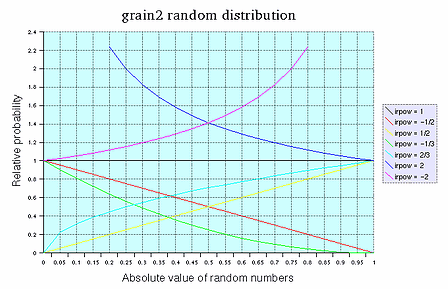
\includegraphics[scale=1]{grain2_rand-448x289} 


 A graph of distributions for different values of irpow.


 \emph{iseed}
 (optional, default=0) -- seed value for random number generator (positive integer in the range 1 to 2147483646 (2 \^{} 31 - 2)). Zero or negative value seeds from current time (this is also the default). 


 \emph{imode}
 (optional default=0) -- sum of the following values: 


 
\begin{itemize}
\item 

 \emph{8:}
 interpolate window waveform (slower).

\item 

 \emph{4:}
 do not interpolate grain waveform (fast, but lower quality).

\item 

 \emph{2:}
 grain frequency is continuously modified by \emph{kcps}
 and \emph{kfmd}
 (by default, each grain keeps the frequency it was launched with). This may be slower at high control rates.

\item 

 \emph{1:}
 skip initialization.


\end{itemize}


 


 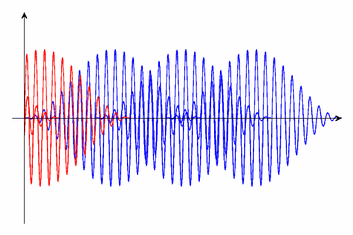
\includegraphics[scale=1]{grain3_2} 


 A diagram showing grains with a start time less than zero in red.
\subsection*{Performance}


 \emph{ar}
 -- output signal. 


 \emph{kcps}
 -- grain frequency in Hz. 


 \emph{kfmd}
 -- random variation (bipolar) in grain frequency in Hz. 


 \emph{kgdur}
 -- grain duration in seconds. \emph{kgdur}
 also controls the duration of already active grains (actually the speed at which the window function is read). This behavior does not depend on the \emph{imode}
 flags. 


 \emph{kfn}
 -- function table containing grain waveform. Table number can be changed at k-rate (this is useful to select from a set of band-limited tables generated by GEN30, to avoid aliasing). 


 


\begin{tabular}{cc}
\textbf{Note}
 \\
� &

 \emph{grain2}
 internally uses the same random number generator as \emph{rnd31}
. So reading \emph{its documentation}
 is also recommended. 


\end{tabular}

\subsection*{Examples}


  Here is an example of the grain2 opcode. It uses the files \emph{grain2.orc}
 and \emph{grain2.sco}
. 


 \textbf{Example 1. Example of the grain2 opcode.}

\begin{lstlisting}
/* grain2.orc */
sr	=  48000
kr	=  750
ksmps	=  64
nchnls	=  2

/* square wave */
i_	ftgen 1, 0, 4096, 7, 1, 2048, 1, 0, -1, 2048, -1
/* window */
i_	ftgen 2, 0, 16384, 7, 0, 4096, 1, 4096, 0.3333, 8192, 0
/* sine wave */
i_	ftgen 3, 0, 1024, 10, 1
/* room parameters */
i_	ftgen 7, 0, 64, -2, 4, 50, -1, -1, -1, 11,			\
			    1, 26.833, 0.05, 0.85, 10000, 0.8, 0.5, 2,	\
			    1,  1.753, 0.05, 0.85,  5000, 0.8, 0.5, 2,	\
			    1, 39.451, 0.05, 0.85,  7000, 0.8, 0.5, 2,	\
			    1, 33.503, 0.05, 0.85,  7000, 0.8, 0.5, 2,	\
			    1, 36.151, 0.05, 0.85,  7000, 0.8, 0.5, 2,	\
			    1, 29.633, 0.05, 0.85,  7000, 0.8, 0.5, 2

ga01	init 0

/* generate bandlimited square waves */

i0	=  0
loop1:
imaxh	=  sr / (2 * 440.0 * exp (log(2.0) * (i0 - 69) / 12))
i_	ftgen i0 + 256, 0, 4096, -30, 1, 1, imaxh
i0	=  i0 + 1
	if (i0 < 127.5) igoto loop1

	instr 1

p3	=  p3 + 0.2

/* note velocity */
iamp	=  0.0039 + p5 * p5 / 16192
/* vibrato */
kcps	oscili 1, 8, 3
kenv	linseg 0, 0.05, 0, 0.1, 1, 1, 1
/* frequency */
kcps	=  (kcps * kenv * 0.01 + 1) * 440 * exp(log(2) * (p4 - 69) / 12)
/* grain ftable */
kfn	=  int(256 + 69 + 0.5 + 12 * log(kcps / 440) / log(2))
/* grain duration */
kgdur	port 100, 0.1, 20
kgdur	=  kgdur / kcps

a1	grain2 kcps, kcps * 0.02, kgdur, 50, kfn, 2, -0.5, 22, 2
a1	butterlp a1, 3000
a2	grain2 kcps, kcps * 0.02, 4 / kcps, 50, kfn, 2, -0.5, 23, 2
a2	butterbp a2, 12000, 8000
a2	butterbp a2, 12000, 8000
aenv1	linseg 0, 0.01, 1, 1, 1
aenv2	linseg 3, 0.05, 1, 1, 1
aenv3	linseg 1, p3 - 0.2, 1, 0.07, 0, 1, 0

a1	=  aenv1 * aenv3 * (a1 + a2 * 0.7 * aenv2)

ga01	=  ga01 + a1 * 10000 * iamp

	endin

/* output instr */

	instr 81

i1	=  0.000001
aLl, aLh, aRl, aRh	spat3di ga01 + i1*i1*i1*i1, 3.0, 4.0, 0.0, 0.5, 7, 4
ga01	=  0
aLl	butterlp aLl, 800.0
aRl	butterlp aRl, 800.0

	outs aLl + aLh, aRl + aRh

	endin
/* grain2.orc */
        
\end{lstlisting}
\begin{lstlisting}
/* grain2.sco */
t 0 60

i 1 0.0 1.3 60 127
i 1 2.0 1.3 67 127
i 1 4.0 1.3 64 112
i 1 4.0 1.3 72 112

i 81 0 6.4

e
/* grain2.sco */
        
\end{lstlisting}
\subsection*{See Also}


 \emph{grain3}

\subsection*{Credits}


 


 


\begin{tabular}{c}
Author: Istvan Varga

\end{tabular}



 


 New in version 4.15


 Updated April 2002 by Istvan Varga
%\hline 


\begin{comment}
\begin{tabular}{lcr}
Previous &Home &Next \\
grain &Up &grain3

\end{tabular}


\end{document}
\end{comment}

\newpage
\begin{comment}
\documentclass[10pt]{article}
\usepackage{fullpage, graphicx, url}
\setlength{\parskip}{1ex}
\setlength{\parindent}{0ex}
\title{grain3}
\begin{document}


\begin{tabular}{ccc}
The Alternative Csound Reference Manual & & \\
Previous & &Next

\end{tabular}

%\hline 
\end{comment}
\section{grain3}
grain3�--� Generate granular synthesis textures with more user control. \subsection*{Description}


  Generate granular synthesis textures. \emph{grain2}
 is simpler to use but \emph{grain3}
 offers more control. 
\subsection*{Syntax}


 ar \textbf{grain3}
 kcps, kphs, kfmd, kpmd, kgdur, kdens, imaxovr, kfn, iwfn, kfrpow, kprpow [, iseed] [, imode]
\subsection*{Initialization}


 \emph{imaxovr}
 -- maximum number of overlapping grains. The number of overlaps can be calculated by (kdens * kgdur); however, it can be overestimated at no cost in rendering time, and a single overlap uses (depending on system) 16 to 32 bytes of memory. 


 \emph{iwfn}
 -- function table containing window waveform (Use GEN20 to calculate iwfn). 


 \emph{irpow}
 (optional, default=0) -- this value controls the distribution of grain frequency variation. If irpow is positive, the random distribution (x is in the range -1 to 1) is 


 abs(x)�\^{}�((1�/�irpow)�-�1)
; for negative irpow values, it is 

 (1�-�abs(x))�\^{}�((-1�/�irpow)�-�1)
. Setting irpow to -1, 0, or 1 will result in uniform distribution (this is also faster to calculate). The image below shows some examples for irpow. The default value of irpow is 0. 

 


 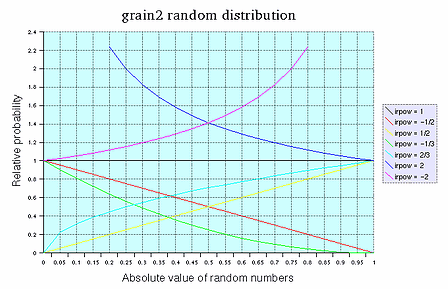
\includegraphics[scale=1]{grain2_rand-448x289} 


 A graph of distributions for different values of irpow.


 \emph{iseed}
 (optional, default=0) -- seed value for random number generator (positive integer in the range 1 to 2147483646 (2 \^{} 31 - 2)). Zero or negative value seeds from current time (this is also the default). 


 \emph{imode}
 (optional, default=0) -- sum of the following values: 


 
\begin{itemize}
\item 

 \emph{64:}
 synchronize start phase of grains to kcps.

\item 

 \emph{32:}
 start all grains at integer sample location. This may be faster in some cases, however it also makes the timing of grain envelopes less accurate.

\item 

 \emph{16:}
 do not render grains with start time less than zero. (see the image below; this option turns off grains marked with red on the image).

\item 

 \emph{8:}
 interpolate window waveform (slower).

\item 

 \emph{4:}
 do not interpolate grain waveform (fast, but lower quality).

\item 

 \emph{2:}
 grain frequency is continuously modified by \emph{kcps}
 and \emph{kfmd}
 (by default, each grain keeps the frequency it was launched with). This may be slower at high control rates. It also controls phase modulation (kphs).

\item 

 \emph{1:}
 skip initialization.


\end{itemize}


 


 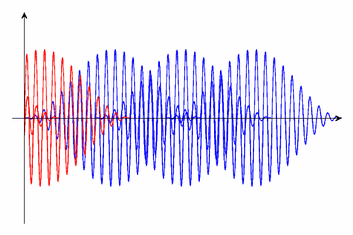
\includegraphics[scale=1]{grain3_2} 


 A diagram showing grains with a start time less than zero in red.
\subsection*{Performance}


 \emph{ar}
 -- output signal. 


 \emph{kcps}
 -- grain frequency in Hz. 


 \emph{kphs}
 -- grain phase. This is the location in the grain waveform table, expressed as a fraction (between 0 to 1) of the table length. 


 \emph{kfmd}
 -- random variation (bipolar) in grain frequency in Hz. 


 \emph{kpmd}
 -- random variation (bipolar) in start phase. 


 \emph{kgdur}
 -- grain duration in seconds. \emph{kgdur}
 also controls the duration of already active grains (actually the speed at which the window function is read). This behavior does not depend on the \emph{imode}
 flags. 


 \emph{kdens}
 -- number of grains per second. 


 \emph{kfrpow}
 -- distribution of random frequency variation (see irpow). 


 \emph{kprpow}
 -- distribution of random phase variation (see irpow). Setting kphs and kpmd to 0.5, and kprpow to 0 will emulate \emph{grain2}
. 


 \emph{kfn}
 -- function table containing grain waveform. Table number can be changed at k-rate (this is useful to select from a set of band-limited tables generated by GEN30, to avoid aliasing). 


 


\begin{tabular}{cc}
\textbf{Note}
 \\
� &

 \emph{grain3}
 internally uses the same random number generator as \emph{rnd31}
. So reading \emph{its documentation}
 is also recommended. 


\end{tabular}

\subsection*{Examples}


  Here is an example of the grain3 opcode. It uses the files \emph{grain3.orc}
 and \emph{grain3.sco}
. 


 \textbf{Example 1. Example of the grain3 opcode.}

\begin{lstlisting}
/* grain3.orc */
sr	=  48000
kr	=  1000
ksmps   =  48
nchnls	=  1

/* Bartlett window */
itmp	ftgen 1, 0, 16384, 20, 3, 1
/* sawtooth wave */
itmp	ftgen 2, 0, 16384, 7, 1, 16384, -1
/* sine */
itmp	ftgen 4, 0, 1024, 10, 1
/* window for "soft sync" with 1/32 overlap */
itmp	ftgen 5, 0, 16384, 7, 0, 256, 1, 7936, 1, 256, 0, 7936, 0
/* generate bandlimited sawtooth waves */
itmp	ftgen 3, 0, 4096, -30, 2, 1, 2048
icnt	=  0
loop01:
; 100 tables for 8 octaves from 30 Hz
ifrq	=  30 * exp(log(2) * 8 * icnt / 100)
itmp	ftgen icnt + 100, 0, 4096, -30, 3, 1, sr / (2 * ifrq)
icnt	=  icnt + 1
	if (icnt < 99.5) igoto loop01
/* convert frequency to table number */
#define FRQ2FNUM(xout'xcps'xbsfn) #

$xout	=  int(($xbsfn) + 0.5 + (100 / 8) * log(($xcps) / 30) / log(2))
$xout	limit $xout, $xbsfn, $xbsfn + 99

#

/* instr 1: pulse width modulated grains */

	instr 1

kfrq	=  523.25		; frequency
$FRQ2FNUM(kfnum'kfrq'100)	; table number
kfmd	=  kfrq * 0.02		; random variation in frequency
kgdur	=  0.2			; grain duration
kdens	=  200			; density
iseed	=  1			; random seed

kphs	oscili 0.45, 1, 4	; phase

a1	grain3	kfrq, 0, kfmd, 0.5, kgdur, kdens, 100,		\
		kfnum, 1, -0.5, 0, iseed, 2
a2	grain3	kfrq, 0.5 + kphs, kfmd, 0.5, kgdur, kdens, 100,	\
		kfnum, 1, -0.5, 0, iseed, 2

; de-click
aenv	linseg 0, 0.01, 1, p3 - 0.05, 1, 0.04, 0, 1, 0

	out aenv * 2250 * (a1 - a2)

	endin

/* instr 2: phase variation */

	instr 2

kfrq	=  220			; frequency
$FRQ2FNUM(kfnum'kfrq'100)	; table number
kgdur	=  0.2			; grain duration
kdens	=  200			; density
iseed	=  2			; random seed

kprdst	expon 0.5, p3, 0.02	; distribution

a1	grain3	kfrq, 0.5, 0, 0.5, kgdur, kdens, 100,		\
		kfnum, 1, 0, -kprdst, iseed, 64

; de-click
aenv	linseg 0, 0.01, 1, p3 - 0.05, 1, 0.04, 0, 1, 0

	out aenv * 1500 * a1

	endin

/* instr 3: "soft sync" */

	instr 3

kdens	=  130.8		; base frequency
kgdur	=  2 / kdens		; grain duration

kfrq	expon 880, p3, 220	; oscillator frequency
$FRQ2FNUM(kfnum'kfrq'100)	; table number

a1	grain3 kfrq, 0, 0, 0, kgdur, kdens, 3, kfnum, 5, 0, 0, 0, 2
a2	grain3 kfrq, 0.667, 0, 0, kgdur, kdens, 3, kfnum, 5, 0, 0, 0, 2

; de-click
aenv	linseg 0, 0.01, 1, p3 - 0.05, 1, 0.04, 0, 1, 0

	out aenv * 10000 * (a1 - a2)

	endin
/* grain3.orc */
        
\end{lstlisting}
\begin{lstlisting}
/* grain3.sco */
t 0 60
i 1 0 3
i 2 4 3
i 3 8 3
e
/* grain3.sco */
        
\end{lstlisting}
\subsection*{See Also}


 \emph{grain2}

\subsection*{Credits}


 


 


\begin{tabular}{c}
Author: Istvan Varga

\end{tabular}



 


 New in version 4.15


 Updated April 2002 by Istvan Varga
%\hline 


\begin{comment}
\begin{tabular}{lcr}
Previous &Home &Next \\
grain2 &Up &granule

\end{tabular}


\end{document}
\end{comment}

\newpage
\begin{comment}
\documentclass[10pt]{article}
\usepackage{fullpage, graphicx, url}
\setlength{\parskip}{1ex}
\setlength{\parindent}{0ex}
\title{granule}
\begin{document}


\begin{tabular}{ccc}
The Alternative Csound Reference Manual & & \\
Previous & &Next

\end{tabular}

%\hline 
\end{comment}
\section{granule}
granule�--� A more complex granular synthesis texture generator. \subsection*{Description}


  The \emph{granule}
 unit generator is more complex than \emph{grain}
, but does add new possibilities. 


 \emph{granule}
 is a Csound unit generator which employs a wavetable as input to produce granularly synthesized audio output. Wavetable data may be generated by any of the GEN subroutines such as \emph{GEN01}
 which reads an audio data file into a wavetable. This enable a sampled sound to be used as the source for the grains. Up to 128 voices are implemented internally. The maximum number of voices can be increased by redefining the variable MAXVOICE in the grain4.h file. \emph{granule}
 has a build-in random number generator to handle all the random offset parameters. Thresholding is also implemented to scan the source function table at initialization stage. This facilitates features such as skipping silence passage between sentences. 


  The characteristics of the synthesis are controlled by 22 parameters. \emph{xamp}
 is the amplitude of the output and it can be either audio rate or control rate variable. 
\subsection*{Syntax}


 ar \textbf{granule}
 xamp, ivoice, iratio, imode, ithd, ifn, ipshift, igskip, igskip\_os, ilength, kgap, igap\_os, kgsize, igsize\_os, iatt, idec [, iseed] [, ipitch1] [, ipitch2] [, ipitch3] [, ipitch4] [, ifnenv]
\subsection*{Performance}


 \emph{xamp}
 -- amplitude. 


 \emph{ivoice}
 -- number of voices. 


 \emph{iratio}
 -- ratio of the speed of the gskip pointer relative to output audio sample rate. eg. 0.5 will be half speed. 


 \emph{imode}
 -- +1 grain pointer move forward (same direction of the gskip pointer), -1 backward (oppose direction to the gskip pointer) or 0 for random. 


 \emph{ithd}
 -- threshold, if the sampled signal in the wavetable is smaller then \emph{ithd}
, it will be skipped. 


 \emph{ifn}
 -- function table number of sound source. 


 \emph{ipshift}
 -- pitch shift control. If \emph{ipshift}
 is 0, pitch will be set randomly up and down an octave. If \emph{ipshift}
 is 1, 2, 3 or 4, up to four different pitches can be set amount the number of voices defined in \emph{ivoice}
. The optional parameters \emph{ipitch1}
, \emph{ipitch2}
, \emph{ipitch3}
 and \emph{ipitch4}
 are used to quantify the pitch shifts. 


 \emph{igskip}
 -- initial skip from the beginning of the function table in sec. 


 \emph{igskip\_os}
 -- gskip pointer random offset in sec, 0 will be no offset. 


 \emph{ilength}
 -- length of the table to be used starting from \emph{igskip}
 in sec. 


 \emph{kgap}
 -- gap between grains in sec. 


 \emph{igap\_os}
 -- gap random offset in \% of the gap size, 0 gives no offset. 


 \emph{kgsize}
 -- grain size in sec. 


 \emph{igsize\_os}
 -- grain size random offset in \% of grain size, 0 gives no offset. 


 \emph{iatt}
 -- attack of the grain envelope in \% of grain size. 


 \emph{idec}
 -- decade of the grain envelope in \% of grain size. 


 \emph{iseed}
 (optional, default=0.5) -- seed for the random number generator. 


 \emph{ipitch1, ipitch2, ipitch3, ipitch4}
 (optional, default=1) -- pitch shift parameter, used when \emph{ipshift}
 is set to 1, 2, 3 or 4. Time scaling technique is used in pitch shift with linear interpolation between data points. Default value is 1, the original pitch. 


 \emph{ifnenv}
 (optional, default=0) -- function table number to be used to generate the shape of the envelope. 
\subsection*{Examples}


  Here is an example of the granule opcode. It uses the files \emph{granule.orc}
, \emph{granule.sco}
, and \emph{mary.wav}
. 


 \textbf{Example 1. Example of the granule opcode.}

\begin{lstlisting}
/* granule.orc */
sr = 44100
kr = 4410
ksmps = 10
nchnls = 2
instr 1
;
k1      linseg 0,0.5,1,(p3-p2-1),1,0.5,0
a1      granule p4*k1,p5,p6,p7,p8,p9,p10,p11,p12,p13,p14,p15,\
        p16,p17,p18,p19,p20,p21,p22,p23,p24
a2      granule p4*k1,p5,p6,p7,p8,p9,p10,p11,p12,p13,p14,p15,\
        p16,p17,p18,p19, p20+0.17,p21,p22,p23,p24
outs a1,a2
endin
/* granule.orc */
        
\end{lstlisting}
\begin{lstlisting}
/* granule.sco */
; f statement read sound file sine.aiff in the SFDIR 
; directory into f-table 1
f1      0 262144 1 "mary.wav" 0 0 0
i1      0 10 2000 64 0.5 0 0 1 4 0 0.005 5 0.01 50 0.02 50 30 30 0.39 \
        1 1.42 0.29 2
e
/* granule.sco */
        
\end{lstlisting}


  The above example reads a sound file called \emph{mary.wav}
 into wavetable number 1 with 262,144 samples. It generates 10 seconds of stereo audio output using the wavetable. In the orchestra file, all parameters required to control the synthesis are passed from the score file. A \emph{linseg}
 function generator is used to generate an envelope with 0.5 second of linear attack and decay. Stereo effect is generated by using different seeds for the two \emph{granule}
 function calls. In the example, 0.17 is added to p20 before passing into the second \emph{granule}
 call to ensure that all of the random offset events are different from the first one. 


  In the score file, the parameters are interpreted as: 


 


\begin{tabular}{|c|c|c|c|c|c|c|c|c|c|c|c|c|}
%\hline 
ParameterInterpreted As & & & & & & & & & & & & \\
 %\hline 
p5 (\emph{ivoice}
)the number of voices is set to 64 &p6 (\emph{iratio}
)set to 0.5, it scans the wavetable at half of the speed of the audio output rate &p7 (\emph{imode}
)set to 0, the grain pointer only move forward &p8 (\emph{ithd}
)set to 0, skipping the thresholding process &p9 (\emph{ifn}
)set to 1, function table number 1 is used &p10 (\emph{ipshift}
)set to 4, four different pitches are going to be generated &p11 (\emph{igskip}
)set to 0 and p12 (igskip\_os) is set to 0.005, no skipping into the wavetable and a 5 mSec random offset is used &p13 (\emph{ilength}
)set to 5, 5 seconds of the wavetable is to be used &p14 (\emph{kgap}
)set to 0.01 and p15 (igap\_os) is set to 50, 10 mSec gap with 50\% random offset is to be used &p16 (\emph{kgsize}
)set to 0.02 and p17 (igsize\_os) is set to 50, 20 mSec grain with 50\% random offset is used &p18 (\emph{iatt}
) and p19 (\emph{idec}
)set to 30, 30\% of linear attack and decade is applied to the grain &p20 (\emph{iseed}
)seed for the random number generator is set to 0.39 &p21 - p24pitches set to 1 which is the original pitch, 1.42 which is a 5th up, 0.29 which is a 7th down and finally 2 which is an octave up. \\
 %\hline 

\end{tabular}



 
\subsection*{Credits}


 


 


\begin{tabular}{ccc}
Author: Allan Lee &Belfast &1996

\end{tabular}



 
%\hline 


\begin{comment}
\begin{tabular}{lcr}
Previous &Home &Next \\
grain3 &Up &guiro

\end{tabular}


\end{document}
\end{comment}

\newpage
\begin{comment}
\documentclass[10pt]{article}
\usepackage{fullpage, graphicx, url}
\setlength{\parskip}{1ex}
\setlength{\parindent}{0ex}
\title{$>$=}
\begin{document}


\begin{tabular}{ccc}
The Alternative Csound Reference Manual & & \\
Previous & &Next

\end{tabular}

%\hline 
\end{comment}
\section{$>$=}
$>$=�--� Determines if one value is greater than or equal to another. \subsection*{Description}


  Determines if one value is greater than or equal to another. 
\subsection*{Syntax}


 (a \textbf{$>$=}
 b \textbf{?}
 v1 \textbf{:}
 v2)


  where \emph{a}
, \emph{b}
, \emph{v1}
 and \emph{v2}
 may be expressions, but \emph{a}
, \emph{b}
 not audio-rate. 
\subsection*{Performance}


  In the above conditionals, \emph{a}
 and \emph{b}
 are first compared. If the indicated relation is true (\emph{a}
 greater than \emph{b}
, \emph{a}
 less than \emph{b}
, \emph{a}
 greater than or equal to \emph{b}
, \emph{a}
 less than or equal to \emph{b}
, \emph{a}
 equal to \emph{b}
, \emph{a}
 not equal to \emph{b}
), then the conditional expression has the value of \emph{v1}
; if the relation is false, the expression has the value of \emph{v2}
. (For convenience, a sole ``\emph{=}
`` will function as ``\emph{= =}
``.) 


  NB.: If \emph{v1}
 or \emph{v2}
 are expressions, these will be evaluated before the conditional is determined. 


  In terms of binding strength, all conditional operators (i.e. the relational operators (\emph{$<$}
, etc.), and \emph{?}
, and \emph{:}
 ) are weaker than the arithmetic and logical operators (\emph{+}
, \emph{-}
, \emph{*}
, \emph{/}
, \emph{\&}
 and \emph{||}
). 


  These are \emph{operators}
 not \emph{opcodes}
. Therefore, they can be used within orchestra statements, but do not form complete statements themselves. 
\subsection*{Examples}


  Here is an example of the $>$= opcode. It uses the files \emph{greaterequal.orc}
 and \emph{greaterequal.sco}
. 


 \textbf{Example 1. Example of the $>$= opcode.}

\begin{lstlisting}
/* greaterequal.orc */
; Initialize the global variables.
sr = 44100
kr = 44100
ksmps = 1
nchnls = 1

; Instrument #1.
instr 1
  ; Get the 4th p-field from the score.
  k1 =  p4

  ; Is it greater than or equal to 3? (1 = true, 0 = false)
  k2 = (p4 >= 3 ? 1 : 0)

  ; Print the values of k1 and k2.
  printks "k1 = %f, k2 = %f\\n", 1, k1, k2
endin
/* greaterequal.orc */
        
\end{lstlisting}
\begin{lstlisting}
/* greaterequal.sco */
; Call Instrument #1 with a p4 = 2.
i 1 0 0.5 2
; Call Instrument #1 with a p4 = 3.
i 1 1 0.5 3
; Call Instrument #1 with a p4 = 4.
i 1 2 0.5 4
e
/* greaterequal.sco */
        
\end{lstlisting}
 Its output should include lines like this: \begin{lstlisting}
k1 = 2.000000, k2 = 0.000000
k1 = 3.000000, k2 = 1.000000
k1 = 4.000000, k2 = 1.000000
      
\end{lstlisting}
\subsection*{See Also}


 \emph{==}
, \emph{$>$}
, \emph{$<$=}
, \emph{$<$}
, \emph{!=}

\subsection*{Credits}


 Example written by Kevin Conder.
%\hline 


\begin{comment}
\begin{tabular}{lcr}
Previous &Home &Next \\
$>$ &Up &$<$

\end{tabular}


\end{document}
\end{comment}

\newpage
\begin{comment}
\documentclass[10pt]{article}
\usepackage{fullpage, graphicx, url}
\setlength{\parskip}{1ex}
\setlength{\parindent}{0ex}
\title{$>$}
\begin{document}


\begin{tabular}{ccc}
The Alternative Csound Reference Manual & & \\
Previous & &Next

\end{tabular}

%\hline 
\end{comment}
\section{$>$}
$>$�--� Determines if one value is greater than another. \subsection*{Description}


  Determines if one value is greater than another. 
\subsection*{Syntax}


 (a \textbf{$>$}
 b \textbf{?}
 v1 \textbf{:}
 v2)


  where \emph{a}
, \emph{b}
, \emph{v1}
 and \emph{v2}
 may be expressions, but \emph{a}
, \emph{b}
 not audio-rate. 
\subsection*{Performance}


  In the above conditionals, \emph{a}
 and \emph{b}
 are first compared. If the indicated relation is true (\emph{a}
 greater than \emph{b}
, \emph{a}
 less than \emph{b}
, \emph{a}
 greater than or equal to \emph{b}
, \emph{a}
 less than or equal to \emph{b}
, \emph{a}
 equal to \emph{b}
, \emph{a}
 not equal to \emph{b}
), then the conditional expression has the value of \emph{v1}
; if the relation is false, the expression has the value of \emph{v2}
. (For convenience, a sole ``\emph{=}
`` will function as ``\emph{= =}
``.) 


  NB.: If \emph{v1}
 or \emph{v2}
 are expressions, these will be evaluated before the conditional is determined. 


  In terms of binding strength, all conditional operators (i.e. the relational operators (\emph{$<$}
, etc.), and \emph{?}
, and \emph{:}
 ) are weaker than the arithmetic and logical operators (\emph{+}
, \emph{-}
, \emph{*}
, \emph{/}
, \emph{\&}
 and \emph{||}
). 


  These are \emph{operators}
 not \emph{opcodes}
. Therefore, they can be used within orchestra statements, but do not form complete statements themselves. 
\subsection*{Examples}


  Here is an example of the $>$ opcode. It uses the files \emph{greaterthan.orc}
 and \emph{greaterthan.sco}
. 


 \textbf{Example 1. Example of the $>$ opcode.}

\begin{lstlisting}
/* greaterthan.orc */
; Initialize the global variables.
sr = 44100
kr = 44100
ksmps = 1
nchnls = 1

; Instrument #1.
instr 1
  ; Get the 4th p-field from the score.
  k1 =  p4

  ; Is it greater than 3? (1 = true, 0 = false)
  k2 = (p4 > 3 ? 1 : 0)

  ; Print the values of k1 and k2.
  printks "k1 = %f, k2 = %f\\n", 1, k1, k2
endin
/* greaterthan.orc */
        
\end{lstlisting}
\begin{lstlisting}
/* greaterthan.sco */
; Call Instrument #1 with a p4 = 2.
i 1 0 0.5 2
; Call Instrument #1 with a p4 = 3.
i 1 1 0.5 3
; Call Instrument #1 with a p4 = 4.
i 1 2 0.5 4
e
/* greaterthan.sco */
        
\end{lstlisting}
 Its output should include lines like this: \begin{lstlisting}
k1 = 2.000000, k2 = 0.000000
k1 = 3.000000, k2 = 0.000000
k1 = 4.000000, k2 = 1.000000
      
\end{lstlisting}
\subsection*{See Also}


 \emph{==}
, \emph{$>$=}
, \emph{$<$=}
, \emph{$<$}
, \emph{!=}

\subsection*{Credits}


 Example written by Kevin Conder.
%\hline 


\begin{comment}
\begin{tabular}{lcr}
Previous &Home &Next \\
\&\& &Up &$>$=

\end{tabular}


\end{document}
\end{comment}

\newpage
\begin{comment}
\documentclass[10pt]{article}
\usepackage{fullpage, graphicx, url}
\setlength{\parskip}{1ex}
\setlength{\parindent}{0ex}
\title{guiro}
\begin{document}


\begin{tabular}{ccc}
The Alternative Csound Reference Manual & & \\
Previous & &Next

\end{tabular}

%\hline 
\end{comment}
\section{guiro}
guiro�--� Semi-physical model of a guiro sound. \subsection*{Description}


 \emph{guiro}
 is a semi-physical model of a guiro sound. It is one of the PhISEM percussion opcodes. PhISEM (Physically Informed Stochastic Event Modeling) is an algorithmic approach for simulating collisions of multiple independent sound producing objects. 
\subsection*{Syntax}


 ar \textbf{guiro}
 kamp, idettack [, inum] [, idamp] [, imaxshake] [, ifreq] [, ifreq1]
\subsection*{Initialization}


 \emph{idettack}
 -- period of time over which all sound is stopped 


 \emph{inum}
 (optional) -- The number of beads, teeth, bells, timbrels, etc. If zero, the default value is 128. 


 \emph{idamp}
 (optional) -- the damping factor of the instrument. \emph{Not used.}



 \emph{imaxshake}
 (optional, default=0) -- amount of energy to add back into the system. The value should be in range 0 to 1. 


 \emph{ifreq}
 (optional) -- the main resonant frequency. The default value is 2500. 


 \emph{ifreq1}
 (optional) -- the first resonant frequency. 
\subsection*{Performance}


 \emph{kamp}
 -- Amplitude of output. Note: As these instruments are stochastic, this is only an approximation. 
\subsection*{Examples}


  Here is an example of the guiro opcode. It uses the files \emph{guiro.orc}
 and \emph{guiro.sco}
. 


 \textbf{Example 1. Example of the guiro opcode.}

\begin{lstlisting}
/* guiro.orc */
sr = 44100
kr = 4410
ksmps = 10
nchnls = 1

    instr 01  ;example of a guiro
a1  guiro p4, 0.01
    out a1
    endin
/* guiro.orc */
        
\end{lstlisting}
\begin{lstlisting}
/* guiro.sco */
i1 0 1 20000
e
/* guiro.sco */
        
\end{lstlisting}
\subsection*{See Also}


 \emph{bamboo}
, \emph{dripwater}
, \emph{sleighbells}
, \emph{tambourine}

\subsection*{Credits}


 


 


\begin{tabular}{cccc}
Author: Perry Cook, part of the PhISEM (Physically Informed Stochastic Event Modeling) &Adapted by John ffitch &University of Bath, Codemist Ltd. &Bath, UK

\end{tabular}



 


 New in Csound version 4.07


 Added notes by Rasmus Ekman on May 2002.
%\hline 


\begin{comment}
\begin{tabular}{lcr}
Previous &Home &Next \\
granule &Up &harmon

\end{tabular}


\end{document}
\end{comment}

\newpage
\begin{comment}
\documentclass[10pt]{article}
\usepackage{fullpage, graphicx, url}
\setlength{\parskip}{1ex}
\setlength{\parindent}{0ex}
\title{harmon}
\begin{document}


\begin{tabular}{ccc}
The Alternative Csound Reference Manual & & \\
Previous & &Next

\end{tabular}

%\hline 
\end{comment}
\section{harmon}
harmon�--� Analyze an audio input and generate harmonizing voices in synchrony. \subsection*{Description}


  Analyze an audio input and generate harmonizing voices in synchrony. 
\subsection*{Syntax}


 ar \textbf{harmon}
 asig, kestfrq, kmaxvar, kgenfreq1, kgenfreq2, imode, iminfrq, iprd
\subsection*{Initialization}


 \emph{imode}
 -- interpreting mode for the generating frequency inputs \emph{kgenfreq1}
, \emph{kgenfreq2}
. 0: input values are ratios with respect to the audio signal analyzed frequency. 1: input values are the actual requested frequencies in Hz. 


 \emph{iminfrq}
 -- the lowest expected frequency (in Hz) of the audio input. This parameter determines how much of the input is saved for the running analysis, and sets a lower bound on the internal pitch tracker. 


 \emph{iprd}
 -- period of analysis (in seconds). Since the internal pitch analysis can be time-consuming, the input is typically analyzed only each 20 to 50 milliseconds. 
\subsection*{Performance}


 \emph{kestfrq}
 -- estimated frequency of the input. 


 \emph{kmaxvar}
 -- the maximum variance. 


 \emph{kgenfreq1}
 -- the first generated frequency. 


 \emph{kgenfreq2}
 -- the second generated frequency. 


  This unit is a harmonizer, able to provide up to two additional voices with the same amplitude and spectrum as the input. The input analysis is assisted by two things: an input estimated frequency \emph{kestfrq}
 (in Hz), and a fractional maximum variance \emph{kmaxvar}
 about that estimate which serves to limit the size of the search. Once the real input frequency is determined, the most recent pulse shape is used to generate the other voices at their requested frequencies. 


  The three frequency inputs can be derived in various ways from a score file or MIDI source. The first is the expected pitch, with a variance parameter allowing for inflections or inaccuracies; if the expected pitch is zero the harmonizer will be silent. The second and third pitches control the output frequencies; if either is zero the harmonizer will output only the non-zero request; if both are zero the harmonizer will be silent. When the requested frequency is higher than the input, the process requires additional computation due to overlapped output pulses. This is currently limited for efficiency reasons, with the result that only one voice can be higher than the input at any one time. 


  This unit is useful for supplying a background chorus effect on demand, or for correcting the pitch of a faulty input vocal. There is essentially no delay between input and output. Output includes only the generated parts, and does not include the input. 
\subsection*{Examples}


  Here is an example of the harmon opcode. It uses the files \emph{harmon.orc}
 and \emph{harmon.sco}
. 


 \textbf{Example 1. Example of the harmon opcode.}

\begin{lstlisting}
/* harmon.orc */
; Initialize the global variables.
sr = 44100
kr = 4410
ksmps = 10
nchnls = 1

; Instrument #1.
instr 1
  ; The frequency of the base note.
  inote = 440

  ; Generate the base note.
  avco vco 20000, inote, 1

  kestfrq = inote
  kmaxvar = 200
  
  ; Calculate frequencies 3 semitones above and
  ; below the base note.
  kgenfreq1 = inote * semitone(3)
  kgenfreq2 = inote * semitone(-3)

  imode = 1
  iminfrq = inote - 200
  iprd = 0.1
  
  ; Generate the harmony notes.
  a1 harmon avco, kestfrq, kmaxvar, kgenfreq1, kgenfreq2, \
            imode, iminfrq, iprd

  out a1
endin
/* harmon.orc */
        
\end{lstlisting}
\begin{lstlisting}
/* harmon.sco */
; Table #1, a sine wave.
f 1 0 16384 10 1

; Play Instrument #1 for two seconds.
i 1 0 2
e
/* harmon.sco */
        
\end{lstlisting}
\subsection*{Credits}


 


 


\begin{tabular}{ccc}
Author: Barry L. Vercoe &M.I.T., Cambridge, Mass &1997

\end{tabular}



 


 Example written by Kevin Conder.
%\hline 


\begin{comment}
\begin{tabular}{lcr}
Previous &Home &Next \\
guiro &Up &hilbert

\end{tabular}


\end{document}
\end{comment}

\newpage
\begin{comment}
\documentclass[10pt]{article}
\usepackage{fullpage, graphicx, url}
\setlength{\parskip}{1ex}
\setlength{\parindent}{0ex}
\title{hetro}
\begin{document}


\begin{tabular}{ccc}
The Alternative Csound Reference Manual & & \\
Previous & &Next

\end{tabular}

%\hline 
\end{comment}
\section{hetro}
hetro�--� Decomposes an input soundfile into component sinusoids. \subsection*{Description}


  Hetrodyne filter analysis for the Csound \emph{adsyn}
 generator. 
\subsection*{Syntax}


 \textbf{csound -U hetro}
 [flags] infilename outfilename


 \textbf{hetro}
 [flags] infilename outfilename
\subsection*{Initialization}


 \emph{hetro}
 takes an input soundfile, decomposes it into component sinusoids, and outputs a description of the components in the form of breakpoint amplitude and frequency tracks. Analysis is conditioned by the control flags below. A space is optional between flag and value. 


 \emph{-s srate}
 -- sampling rate of the audio input file. This will over-ride the srate of the soundfile header, which otherwise applies. If neither is present, the default is 10000. Note that for \emph{adsyn}
 synthesis the srate of the source file and the generating orchestra need not be the same. 


 \emph{-c channel}
 -- channel number sought. The default is 1. 


 \emph{-b begin}
 -- beginning time (in seconds) of the audio segment to be analyzed. The default is 0.0 


 \emph{-d duration}
 -- duration (in seconds) of the audio segment to be analyzed. The default of 0.0 means to the end of the file. Maximum length is 32.766 seconds. 


 \emph{-f begfreq}
 -- estimated starting frequency of the fundamental, necessary to initialize the filter analysis. The default is 100 (cps). 


 \emph{-h partials}
 -- number of harmonic partials sought in the audio file. Default is 10, maximum is a function of memory available. 


 \emph{-M maxamp}
 -- maximum amplitude summed across all concurrent tracks. The default is 32767. 


 \emph{-m minamp}
 -- amplitude threshold below which a single pair of amplitude/frequency tracks is considered dormant and will not contribute to output summation. Typical values: 128 (48 db down from full scale), 64 (54 db down), 32 (60 db down), 0 (no thresholding). The default threshold is 64 (54 db down). 


 \emph{-n brkpts}
 -- initial number of analysis breakpoints in each amplitude and frequency track, prior to thresholding (\emph{-m}
) and linear breakpoint consolidation. The initial points are spread evenly over the duration. The default is 256. 


 \emph{-l cutfreq}
 -- substitute a 3rd order Butterworth low-pass filter with cutoff frequency \emph{cutfreq}
 (in Hz), in place of the default averaging comb filter. The default is 0 (don't use). 
\subsection*{Performance}


  As of Csound 4.08, \emph{hetro}
 can write SDIF ouput files if the output file name ends with ``.sdif''. See the \emph{sdif2ad utility}
 for more information about the Csound's SDIF support. 
\subsection*{Examples}


 


 
\begin{lstlisting}
\emph{hetro}
 -s44100 -b.5 -d2.5 -h16 -M24000 audiofile.test adsynfile7
        
\end{lstlisting}


 
 This will analyze 2.5 seconds of channel 1 of a file ``audiofile.test'', recorded at 44.1 kHz, beginning .5 seconds from the start, and place the result in a file ``adsynfile7''. We request just the first 16 harmonics of the sound, with 256 initial breakpoint values per amplitude or frequency track, and a peak summation amplitude of 24000. The fundamental is estimated to begin at 100 Hz. Amplitude thresholding is at 54 db down. 

  The Butterworth LPF is not enabled. 
\subsubsection*{File Format}


  The output file contains time-sequenced amplitude and frequency values for each partial of an additive complex audio source. The information is in the form of breakpoints (time, value, time, value, ....) using 16-bit integers in the range 0 - 32767. Time is given in milliseconds, and frequency in Hertz (cps). The breakpoint data is exclusively non-negative, and the values -1 and -2 uniquely signify the start of new amplitude and frequency tracks. A track is terminated by the value 32767. Before being written out, each track is data-reduced by amplitude thresholding and linear breakpoint consolidation. 


  A component partial is defined by two breakpoint sets: an amplitude set, and a frequency set. Within a composite file these sets may appear in any order (amplitude, frequency, amplitude ....; or amplitude, amplitude..., then frequency, frequency,...). During \emph{adsyn}
 resynthesis the sets are automatically paired (amplitude, frequency) from the order in which they were found. There should be an equal number of each. 


  A legal \emph{adsyn}
 control file could have following format: 


 
\begin{lstlisting}
-1 time1 value1 ... timeK valueK 32767 ; amplitude breakpoints for partial 1
-2 time1 value1 ... timeL valueL 32767 ; frequency breakpoints for partial 1
-1 time1 value1 ... timeM valueM 32767 ; amplitude breakpoints for partial 2
-2 time1 value1 ... timeN valueN 32767 ; frequency breakpoints for partial 2
-2 time1 value1 ..........
-2 time1 value1 ..........             ; pairable tracks for partials 3 and 4
-1 time1 value1 ..........
-1 time2 value1 ..........
          
\end{lstlisting}


 
\subsection*{Credits}


  October 2002. Thanks to Rasmus Ekman, added a note about the SDIF format. 
%\hline 


\begin{comment}
\begin{tabular}{lcr}
Previous &Home &Next \\
Analysis File Generation &Up &lpanal

\end{tabular}


\end{document}
\end{comment}

\newpage
\begin{comment}
\documentclass[10pt]{article}
\usepackage{fullpage, graphicx, url}
\setlength{\parskip}{1ex}
\setlength{\parindent}{0ex}
\title{hilbert}
\begin{document}


\begin{tabular}{ccc}
The Alternative Csound Reference Manual & & \\
Previous & &Next

\end{tabular}

%\hline 
\end{comment}
\section{hilbert}
hilbert�--� A Hilbert transformer. \subsection*{Description}


  An IIR implementation of a Hilbert transformer. 
\subsection*{Syntax}


 ar1, ar2 \textbf{hilbert}
 asig
\subsection*{Performance}


 \emph{asig}
 -- input signal 


 \emph{ar1}
 -- cosine output of \emph{asig}



 \emph{ar2}
 -- sine output of \emph{asig}



 \emph{hilbert}
 is an IIR filter based implementation of a broad-band 90 degree phase difference network. The input to \emph{hilbert}
 is an audio signal, with a frequency range from 15 Hz to 15 kHz. The outputs of \emph{hilbert}
 have an identical frequency response to the input (i.e. they sound the same), but the two outputs have a constant phase difference of 90 degrees, plus or minus some small amount of error, throughout the entire frequency range. The outputs are in quadrature. 


 \emph{hilbert}
 is useful in the implementation of many digital signal processing techniques that require a signal in phase quadrature. \emph{ar1}
 corresponds to the cosine output of \emph{hilbert}
, while \emph{ar2}
 corresponds to the sine output. The two outputs have a constant phase difference throughout the audio range that corresponds to the phase relationship between cosine and sine waves. 


  Internally, \emph{hilbert}
 is based on two parallel 6th-order allpass filters. Each allpass filter implements a phase lag that increases with frequency; the difference between the phase lags of the parallel allpass filters at any given point is approximately 90 degrees. 


  Unlike an FIR-based Hilbert transformer, the output of \emph{hilbert}
 does not have a linear phase response. However, the IIR structure used in \emph{hilbert}
 is far more efficient to compute, and the nonlinear phase response can be used in the creation of interesting audio effects, as in the second example below. 
\subsection*{Examples}


  The first example implements frequency shifting, or single sideband amplitude modulation. Frequency shifting is similar to ring modulation, except the upper and lower sidebands are separated into individual outputs. By using only one of the outputs, the input signal can be ``detuned,'' where the harmonic components of the signal are shifted out of harmonic alignment with each other, e.g. a signal with harmonics at 100, 200, 300, 400 and 500 Hz, shifted up by 50 Hz, will have harmonics at 150, 250, 350, 450, and 550 Hz. 


  Here is the first example of the hilbert opcode. It uses the files \emph{hilbert.orc}
, \emph{hilbert.sco}
, and \emph{mary.wav}
. 


 \textbf{Example 1. Example of the hilbert opcode implementing frequency shifting.}

\begin{lstlisting}
/* hilbert.orc */
sr = 44100
kr = 4410
ksmps = 10
nchnls = 1
  
instr 1
  idur = p3
  ; Initial amount of frequency shift.
  ; It can be positive or negative.
  ibegshift = p4 
  ; Final amount of frequency shift.
  ; It can be positive or negative.
  iendshift = p5 
  
  ; A simple envelope for determining the 
  ; amount of frequency shift.
  kfreq linseg ibegshift, idur, iendshift
 
  ; Use the sound of your choice.
  ain soundin "mary.wav"
 
  ; Phase quadrature output derived from input signal.
  areal, aimag hilbert ain
 
  ; Quadrature oscillator.
  asin oscili 1, kfreq, 1
  acos oscili 1, kfreq, 1, .25
 
  ; Use a trigonometric identity. 
  ; See the references for further details.
  amod1 = areal * acos
  amod2 = aimag * asin

  ; Both sum and difference frequencies can be 
  ; output at once.
  ; aupshift corresponds to the sum frequencies.
  aupshift = (amod1 + amod2) * 0.7
  ; adownshift corresponds to the difference frequencies. 
  adownshift = (amod1 - amod2) * 0.7

  ; Notice that the adding of the two together is
  ; identical to the output of ring modulation.

  out aupshift
endin
/* hilbert.orc */
        
\end{lstlisting}
\begin{lstlisting}
/* hilbert.sco */
; Sine table for quadrature oscillator.
f 1 0 16384 10 1

; Starting with no shift, ending with all
; frequencies shifted up by 200 Hz.
i 1 0 2 0 200

; Starting with no shift, ending with all
; frequencies shifted down by 200 Hz.
i 1 2 2 0 -200
e
/* hilbert.sco */
        
\end{lstlisting}


  The second example is a variation of the first, but with the output being fed back into the input. With very small shift amounts (i.e. between 0 and +-6 Hz), the result is a sound that has been described as a ``barberpole phaser'' or ``Shepard tone phase shifter.'' Several notches appear in the spectrum, and are constantly swept in the direction opposite that of the shift, producing a filtering effect that is reminiscent of Risset's ``endless glissando''. 


  Here is the second example of the hilbert opcode. It uses the files \emph{hilbert\_barberpole.orc}
, \emph{hilbert\_barberpole.sco}
, and \emph{mary.wav}
. 


 \textbf{Example 2. Example of the hilbert opcode sounding like a ``barberpole phaser''.}

\begin{lstlisting}
/* hilbert_barberpole.orc */
; Initialize the global variables.
sr = 44100
; kr must equal sr for the barberpole effect to work.
kr = 44100
ksmps = 1
nchnls = 2

; Instrument #1
instr 1
  idur = p3
  ibegshift = p4
  iendshift = p5

  ; sawtooth wave, not bandlimited
  asaw   phasor 100
  ; add offset to center phasor amplitude between -.5 and .5
  asaw = asaw - .5
  ; sawtooth wave, with amplitude of 10000
  ain = asaw * 20000
  
  ; The envelope of the frequency shift.
  kfreq linseg ibegshift, idur, iendshift

  ; Phase quadrature output derived from input signal.
  areal, aimag hilbert ain

  ; The quadrature oscillator.
  asin oscili 1, kfreq, 1
  acos oscili 1, kfreq, 1, .25

  ; Based on trignometric identities.
  amod1 = areal * acos
  amod2 = aimag * asin

  ; Calculate the up-shift and down-shift.
  aupshift = (amod1 + amod2) * 0.7
  adownshift = (amod1 - amod2) * 0.7

  ; Mix in the original signal to achieve the barberpole effect.
  amix1 = aupshift + ain
  amix2 = aupshift + ain
  
  ; Make sure the output doesn't get louder than the original signal.
  aout1 balance amix1, ain
  aout2 balance amix2, ain

  outs aout1, aout2
endin
/* hilbert_barberpole.orc */
        
\end{lstlisting}
\begin{lstlisting}
/* hilbert_barberpole.sco */
; Table 1: A sine wave for the quadrature oscillator.
f 1 0 16384 10 1

; The score.
; p4 = frequency shifter, starting frequency.
; p5 = frequency shifter, ending frequency.
i 1 0 6 -10 10
e
/* hilbert_barberpole.sco */
        
\end{lstlisting}
\subsection*{Technical History}


  The use of phase-difference networks in frequency shifters was pioneered by Harald Bode.1 Bode and Bob Moog provide an excellent description of the implementation and use of a frequency shifter in the analog realm in;2 this would be an excellent first source for those that wish to explore the possibilities of single sideband modulation. Bernie Hutchins provides more applications of the frequency shifter, as well as a detailed technical analysis.3 A recent paper by Scott Wardle4 describes a digital implementation of a frequency shifter, as well as some unique applications. 
\subsection*{References}


 


 
\begin{enumerate}
\item 

  H. Bode, ``Solid State Audio Frequency Spectrum Shifter.'' AES Preprint No. 395 (1965). 

\item 

  H. Bode and R.A. Moog, ``A High-Accuracy Frequency Shfiter for Professional Audio Applications.'' \emph{Journal of the Audio Engineering Society}
, July/August 1972, vol. 20, no. 6, p. 453. 

\item 

  B. Hutchins. \emph{Musical Engineer's Handbook}
 (Ithaca, NY: Electronotes, 1975), ch. 6a. 

\item 

  S. Wardle, ``A Hilbert-Transformer Frequency Shifter for Audio.'' Available online at \emph{\url{http://www.iua.upf.es/dafx98/papers/}}
. 


\end{enumerate}
\subsection*{Credits}


 


 


\begin{tabular}{ccc}
Author: Sean Costello &Seattle, Washington &1999

\end{tabular}



 


 New in Csound version 3.55


 The examples were updated April 2002. Thanks go to Sean Costello for fixing the barberpole example.
%\hline 


\begin{comment}
\begin{tabular}{lcr}
Previous &Home &Next \\
harmon &Up &hrtfer

\end{tabular}


\end{document}
\end{comment}

\newpage
\begin{comment}
\documentclass[10pt]{article}
\usepackage{fullpage, graphicx, url}
\setlength{\parskip}{1ex}
\setlength{\parindent}{0ex}
\title{hrtfer}
\begin{document}


\begin{tabular}{ccc}
The Alternative Csound Reference Manual & & \\
Previous & &Next

\end{tabular}

%\hline 
\end{comment}
\section{hrtfer}
hrtfer�--� Creates 3D audio for two speakers. \subsection*{Description}


  Output is binaural (headphone) 3D audio. 
\subsection*{Syntax}


 aleft, aright \textbf{hrtfer}
 asig, kaz, kelev, ``HRTFcompact''
\subsection*{Initialization}


 \emph{kAz}
 -- azimuth value in degrees. Positive values represent position on the right, negative values are positions on the left. 


 \emph{kElev}
 -- elevation value in degrees. Positive values represent position above horizontal, negative values are positions above horizontal. 


  At present, the only file which can be used with \emph{hrtfer}
 is \emph{HRTFcompact}
. It must be passed to the opcode as the last argument within quotes as shown above. 


  HRTFcompact may also be obtained via anonymous ftp from: \emph{\url{ftp://ftp.cs.bath.ac.uk/pub/dream/utilities/Analysis/HRTFcompact}}

\subsection*{Performance}


  These unit generators place a mono input signal in a virtual 3D space around the listener by convolving the input with the appropriate HRTF data specified by the opcode's azimuth and elevation values. \emph{hrtfer}
 allows these values to be k-values, allowing for dynamic spatialization. \emph{hrtfer}
 can only place the input at the requested position because the HRTF is loaded in at i-time (remember that currently, CSound has a limit of 20 files it can hold in memory, otherwise it causes a segmentation fault). The output will need to be scaled either by using balance or by multiplying the output by some scaling constant. 


 


\begin{tabular}{cc}
\textbf{Note}
 \\
� &

  The sampling rate of the orchestra must be 44.1kHz. This is because 44.1kHz is the sampling rate at which the HRTFs were measured. In order to be used at a different rate, the HRTFs would need to be re-sampled at the desired rate. 


\end{tabular}

\subsection*{Examples}


  Here is an example of the hrtfer opcode. It uses the files \emph{hrtfer.orc}
, \emph{hrtfer.sco}
, \emph{HRTFcompact}
, and \emph{beats.wav}
. 


 \textbf{Example 1. Example of the hrtfer opcode.}

\begin{lstlisting}
/* hrtfer.orc */
; Initialize the global variables.
sr = 44100
kr = 4410
ksmps = 10
nchnls = 2

instr 1
  kaz          linseg 0, p3, -360  ; move the sound in circle
  kel          linseg -40, p3, 45  ; around the listener, changing
                                    ; elevation as its turning
  asrc         soundin "beats.wav"
  aleft,aright hrtfer asrc, kaz, kel, "HRTFcompact"
  aleftscale   = aleft * 200
  arightscale  = aright * 200

  outs         aleftscale, arightscale
endin        
/* hrtfer.orc */
        
\end{lstlisting}
\begin{lstlisting}
/* hrtfer.sco */
i 1 0 2
e
/* hrtfer.sco */
        
\end{lstlisting}
\subsection*{Credits}


 


 


\begin{tabular}{ccc}
Authors: Eli Breder and David MacIntyre &Montreal &1996

\end{tabular}



 


 Fixed the example thanks to a message from Istvan Varga.
%\hline 


\begin{comment}
\begin{tabular}{lcr}
Previous &Home &Next \\
hilbert &Up &hsboscil

\end{tabular}


\end{document}
\end{comment}

\newpage
\begin{comment}
\documentclass[10pt]{article}
\usepackage{fullpage, graphicx, url}
\setlength{\parskip}{1ex}
\setlength{\parindent}{0ex}
\title{hsboscil}
\begin{document}


\begin{tabular}{ccc}
The Alternative Csound Reference Manual & & \\
Previous & &Next

\end{tabular}

%\hline 
\end{comment}
\section{hsboscil}
hsboscil�--� An oscillator which takes tonality and brightness as arguments. \subsection*{Description}


  An oscillator which takes tonality and brightness as arguments, relative to a base frequency. 
\subsection*{Syntax}


 ar \textbf{hsboscil}
 kamp, ktone, kbrite, ibasfreq, iwfn, ioctfn [, ioctcnt] [, iphs]
\subsection*{Initialization}


 \emph{ibasfreq}
 -- base frequency to which tonality and brighness are relative 


 \emph{iwfn}
 -- function table of the waveform, usually a sine 


 \emph{ioctfn}
 -- function table used for weighting the octaves, usually something like: 


 f1�0��1024��-19��1��0.5��270��0.5\\ 
 ������


 \emph{ioctcnt}
 (optional) -- number of octaves used for brightness blending. Must be in the range 2 to 10. Default is 3. 


 \emph{iphs}
 (optional, default=0) -- initial phase of the oscillator. If \emph{iphs}
 = -1, initialization is skipped. 
\subsection*{Performance}


 \emph{kamp}
 -- amplitude of note 


 \emph{ktone}
 -- cyclic tonality parameter relative to \emph{ibasfreq}
 in logarithmic octave, range 0 to 1, values $>$ 1 can be used, and are internally reduced to \emph{frac}
(\emph{ktone}
). 


 \emph{kbrite}
 -- brightness parameter relative to \emph{ibasfreq}
, achieved by weighting \emph{ioctcnt}
 octaves. It is scaled in such a way, that a value of 0 corresponds to the orignal value of \emph{ibasfreq}
, 1 corresponds to one octave above \emph{ibasfreq}
, -2 corresponds to two octaves below \emph{ibasfreq}
, etc. \emph{kbrite}
 may be fractional. 


 \emph{hsboscil}
 takes tonality and brightness as arguments, relative to a base frequency (\emph{ibasfreq}
). Tonality is a cyclic parameter in the logarithmic octave, brightness is realized by mixing multiple weighted octaves. It is useful when tone space is understood in a concept of polar coordinates. 


  Making \emph{ktone}
 a line, and \emph{kbrite}
 a constant, produces Risset's glissando. 


  Oscillator table \emph{iwfn}
 is always read interpolated. Performance time requires about \emph{ioctcnt}
 * \emph{oscili}
. 
\subsection*{Examples}


  Here is an example of the hsboscil opcode. It uses the files \emph{hsboscil.orc}
 and \emph{hsboscil.sco}
. 


 \textbf{Example 1. Example of the hsboscil opcode.}

\begin{lstlisting}
/* hsboscil.orc */
; Initialize the global variables.
sr = 44100
kr = 4410
ksmps = 10
nchnls = 1

; synth waveform
giwave ftgen 1, 0, 1024, 10, 1, 1, 1, 1
; blending window
giblend ftgen 2, 0, 1024, -19, 1, 0.5, 270, 0.5

; Instrument #1 - produces Risset's glissando.
instr 1
  kamp = 10000
  kbrite = 0.5
  ibasfreq = 200
  ioctcnt = 5

  ; Change ktone linearly from 0 to 1, 
  ; over the period defined by p3.
  ktone line 0, p3, 1

  a1 hsboscil kamp, ktone, kbrite, ibasfreq, giwave, giblend, ioctcnt
  out a1
endin
/* hsboscil.orc */
        
\end{lstlisting}
\begin{lstlisting}
/* hsboscil.sco */
; Play Instrument #1 for ten seconds.
i 1 0 10
e
/* hsboscil.sco */
        
\end{lstlisting}


  Here is an example of the hsboscil opcode in a MIDI instrument. It uses the files \emph{hsboscil\_midi.orc}
 and \emph{hsboscil\_midi.sco}
. 


 \textbf{Example 2. Example of the hsboscil opcode in a MIDI instrument.}

\begin{lstlisting}
/* hsboscil_midi.orc */
; Initialize the global variables.
sr = 44100
kr = 4410
ksmps = 10
nchnls = 1

; synth waveform
giwave ftgen 1, 0, 1024, 10, 1, 1, 1, 1
; blending window
giblend ftgen 2, 0, 1024, -19, 1, 0.5, 270, 0.5

; Instrument #1 - use hsboscil in a MIDI instrument.
instr 1
  ibase = cpsoct(6)
  ioctcnt = 5

  ; all octaves sound alike.
  itona octmidi
  ; velocity is mapped to brightness
  ibrite ampmidi 3

  ; Map an exponential envelope for the amplitude.
  kenv expon 20000, 1, 100

  asig hsboscil kenv, itona, ibrite, ibase, giwave, giblend, ioctcnt
  out asig
endin
/* hsboscil_midi.orc */
        
\end{lstlisting}
\begin{lstlisting}
/* hsboscil_midi.sco */
; Play Instrument #1 for ten minutes
i 1 0 6000
e
/* hsboscil_midi.sco */
        
\end{lstlisting}
\subsection*{Credits}


 


 


\begin{tabular}{ccc}
Author: Peter Neub\"acker &Munich, Germany &August, 1999

\end{tabular}



 


 New in Csound version 3.58
%\hline 


\begin{comment}
\begin{tabular}{lcr}
Previous &Home &Next \\
hrtfer &Up &i

\end{tabular}


\end{document}
\end{comment}

\newpage
%\begin{comment}
\documentclass[10pt]{article}
\usepackage{fullpage, graphicx, url}
\setlength{\parskip}{1ex}
\setlength{\parindent}{0ex}
\title{i Statement (Instrument or Note Statement)}
\begin{document}


\begin{tabular}{ccc}
The Alternative Csound Reference Manual & & \\
Previous & &Next

\end{tabular}

%\hline 
\end{comment}
\section{i Statement (Instrument or Note Statement)}
i�--� Makes an instrument active at a specific time and for a certain duration. \subsection*{Description}


  This statement calls for an instrument to be made active at a specific time and for a certain duration. The parameter field values are passed to that instrument prior to its initialization, and remain valid throughout its Performance. 
\subsection*{Syntax}


 \textbf{i}
 p1 p2 p3 p4 ...
\subsection*{Initialization}


 \emph{p1}
 -- Instrument number, usually a non-negative integer. An optional fractional part can provide an additional tag for specifying ties between particular notes of consecutive clusters. A negative p1 (including tag) can be used to turn off a particular ``held'' note. 


 \emph{p2}
 -- Starting time in arbitrary units called beats. 


 \emph{p3}
 -- Duration time in beats (usually positive). A negative value will initiate a held note (see also \emph{ihold}
). A zero value will invoke an initialization pass without performance (see also \emph{instr}
). 


 \emph{p4 ...}
 -- Parameters whose significance is determined by the instrument. 
\subsection*{Performance}


  Beats are evaluated as seconds, unless there is a \emph{t statement}
 in this score section or a \emph{-t flag}
 in the command-line. 


  Starting or action times are relative to the beginning of a section ( see \emph{s statement}
), which is assigned time 0. 


  Note statements within a section may be placed in any order. Before being sent to an orchestra, unordered score statements must first be processed by Sorter, which will reorder them by ascending p2 value. Notes with the same p2 value will be ordered by ascending p1; if the same p1, then by ascending p3. 


  Notes may be stacked, i.e., a single instrument can perform any number of notes simultaneously. (The necessary copies of the instrument's data space will be allocated dynamically by the orchestra loader.) Each note will normally turn off when its p3 duration has expired, or on receipt of a MIDI noteoff signal. An instrument can modify its own duration either by changing its p3 value during note initialization, or by prolonging itself through the action of a \emph{linenr}
 unit. 


  An instrument may be turned on and left to perform indefinitely either by giving it a negative p3 or by including an \emph{ihold}
 in its i-time code. If a held note is active, an \emph{i statement}
 \emph{with matching p1}
 will not cause a new allocation but will take over the data space of the held note. The new pfields (including p3) will now be in effect, and an i-time pass will be executed in which the units can either be newly initialized or allowed to continue as required for a tied note (see \emph{tigoto}
). A held note may be succeeded either by another held note or by a note of finite duration. A held note will continue to perform across section endings (see \emph{s statement}
). It is halted only by \emph{turnoff}
 or by an \emph{i statement}
 with negative matching p1 or by an \emph{e statement}
. 


  It is possible to have multiple instances (usually, but not necessarily, notes of different pitches) of the same instrument, held simultaneously, via negative p3 values. The instrument can then be fed new parameters from the score. This is useful for avoiding long hard-coded \emph{linseg}
s, and can be accomplished by adding a decimal part to the instrument number. 


  For example, to hold three copies of instrument 10 in a simple chord: 


 
\begin{lstlisting}
i10.1    0    -1    7.00
i10.2    0    -1    7.04
i10.3    0    -1    7.07
        
\end{lstlisting}


 


  Subsequent \emph{i}
 statements can refer to the same sounding note instances, and if the instrument definition is done properly, the new p-fields can be used to alter the character of the notes in progress. For example, to bend the previous chord up an octave and release it: 


 
\begin{lstlisting}
i10.1    1    1    8.00
i10.2    1    1    8.04
i10.3    1    1    8.07
        
\end{lstlisting}


 


  The instrument definition has to take this into account, however, especially if clicks are to be avoided (see the example below). 


  Note that the decimal instrument number notation cannot be used in conjunction with real-time MIDI. In this case, the instrument would be monophonic while a note was held. 


  Notes being tied to previous instances of the same instrument, should skip most initialization by means of \emph{tigoto}
, except for the values entered in score. For example, all table reading opcodes in the instrument, should usually be skipped, as they store their phase internally. If this is suddenly changed, there will be audible clicks in the output. 


  Note that many opcodes (such as \emph{delay}
 and \emph{reverb}
) are prepared for optional initialization. To use this feature, the \emph{tival opcode}
 is suitable. Therefore, they need not be hidden by a \emph{tigoto}
 jump. 


  Beginning with Csound version 3.53, strings are recognized in p-fields for opcodes that accept them (\emph{convolve, adsyn, diskin,}
 etc.). There may be only one string per score line. 
\subsubsection*{Special Considerations}


  The maximum instrument number used to be 200. This has been changed to be limited by memory only (currently there is an internal soft limit of 200; this is automatically extended as required). 
\subsection*{Examples}


  Here is an instrument which can find out whether it is tied to a previous note (\emph{tival}
 returns 1), and whether it is held (negative p3). Attack and release are handled accordingly: 


 
\begin{lstlisting}
\emph{instr}
 10
        
  icps     \emph{init}
      \emph{cpspch}
(p4)                  ;Get target pitch from score event
  iportime \emph{init}
      \emph{abs}
(p3)/7                   ; Portamento time dep on note length
  iamp0    \emph{init}
      p5                          ; Set default amps
  iamp1    \emph{init}
      p5
  iamp2    \emph{init}
      p5
      
  itie     \emph{tival}
                                 ; Check if this note is tied,
  \emph{if}
 itie  ==  1     \emph{igoto}
 nofadein              ; if not fade in
  iamp0    \emph{init}
      0

 nofadein:
  \emph{if}
 p3    < 0       \emph{igoto}
 nofadeout             ; Check if this note is held, if not fade out
  iamp2    \emph{init}
      0    

 nofadeout:
  ; Now do amp from the set values:
  kamp     \emph{linseg}
    iamp0, .03, iamp1, abs(p3)-.03, iamp2
        
  ; Skip rest of initialization on tied note:
           \emph{tigoto}
    tieskip

  kcps     \emph{init}
      icps                        ; Init pitch for untied note
  kcps     \emph{port}
      icps, iportime, icps        ; Drift towards target pitch

  kpw      \emph{oscil}
     .4, rnd(1), 1, rnd(.7)      ; A simple triangle-saw oscil
  ar       \emph{vco}
       kamp, kcps, 3, kpw+.5, 1, 1/icps
        
  ; (Used in testing - one may set ipch to cpspch(p4+2)
  ;       and view output spectrum)
  ;       ar oscil kamp, kcps, 1

          out        ar

 tieskip:                                       ; Skip some initialization on tied note

\emph{endin}

        
\end{lstlisting}


 


  A simple score using three instances of the above instrument: 


 
\begin{lstlisting}
  f1   0 8192 10 1            ; Sine

  i10.1    0    -1    7.00    10000
  i10.2    0    -1    7.04
  i10.3    0    -1    7.07
  i10.1    1    -1    8.00  
  i10.2    1    -1    8.04
  i10.3    1    -1    8.07
  i10.1    2     1    7.11  
  i10.2    2     1    8.04  
  i10.3    2     1    8.07
  e
        
\end{lstlisting}


 
\subsection*{Credits}


  Additional text (Csound Version 4.07) explaining tied notes, edited by Rasmus Ekman from a note by David Kirsh, posted to the Csound mailing list. Example instrument by Rasmus Ekman. 


  Updated August 2002 thanks to a note from Rasmus Ekman. There is no longer a hard limit of 200 instruments. 
%\hline 


\begin{comment}
\begin{tabular}{lcr}
Previous &Home &Next \\
f Statement (or Function Table Statement) &Up &m Statement (Mark Statement)

\end{tabular}


\end{document}
\end{comment}

\begin{comment}
\documentclass[10pt]{article}
\usepackage{fullpage, graphicx, url}
\setlength{\parskip}{1ex}
\setlength{\parindent}{0ex}
\title{ibetarand}
\begin{document}


\begin{tabular}{ccc}
The Alternative Csound Reference Manual & & \\
Previous & &Next

\end{tabular}

%\hline 
\end{comment}
\section{ibetarand}
ibetarand�--� Deprecated. \subsection*{Description}


  Deprecated as of version 3.49. Use the \emph{betarand}
 opcode instead. 
%\hline 


\begin{comment}
\begin{tabular}{lcr}
Previous &Home &Next \\
i &Up &ibexprnd

\end{tabular}


\end{document}
\end{comment}

\newpage
\begin{comment}
\documentclass[10pt]{article}
\usepackage{fullpage, graphicx, url}
\setlength{\parskip}{1ex}
\setlength{\parindent}{0ex}
\title{ibexprnd}
\begin{document}


\begin{tabular}{ccc}
The Alternative Csound Reference Manual & & \\
Previous & &Next

\end{tabular}

%\hline 
\end{comment}
\section{ibexprnd}
ibexprnd�--� Deprecated. \subsection*{Description}


  Deprecated as of version 3.49. Use the \emph{bexprnd}
 opcode instead. 
%\hline 


\begin{comment}
\begin{tabular}{lcr}
Previous &Home &Next \\
ibetarand &Up &icauchy

\end{tabular}


\end{document}
\end{comment}

\newpage
\begin{comment}
\documentclass[10pt]{article}
\usepackage{fullpage, graphicx, url}
\setlength{\parskip}{1ex}
\setlength{\parindent}{0ex}
\title{icauchy}
\begin{document}


\begin{tabular}{ccc}
The Alternative Csound Reference Manual & & \\
Previous & &Next

\end{tabular}

%\hline 
\end{comment}
\section{icauchy}
icauchy�--� Deprecated. \subsection*{Description}


  Deprecated as of version 3.49. Use the \emph{cauchy}
 opcode instead. 
%\hline 


\begin{comment}
\begin{tabular}{lcr}
Previous &Home &Next \\
ibexprnd &Up &ictrl14

\end{tabular}


\end{document}
\end{comment}

\newpage
\begin{comment}
\documentclass[10pt]{article}
\usepackage{fullpage, graphicx, url}
\setlength{\parskip}{1ex}
\setlength{\parindent}{0ex}
\title{ictrl14}
\begin{document}


\begin{tabular}{ccc}
The Alternative Csound Reference Manual & & \\
Previous & &Next

\end{tabular}

%\hline 
\end{comment}
\section{ictrl14}
ictrl14�--� Deprecated. \subsection*{Description}


  Deprecated as of version 3.52. Use the \emph{ctrl14}
 opcode instead. 
%\hline 


\begin{comment}
\begin{tabular}{lcr}
Previous &Home &Next \\
icauchy &Up &ictrl21

\end{tabular}


\end{document}
\end{comment}

\newpage
\begin{comment}
\documentclass[10pt]{article}
\usepackage{fullpage, graphicx, url}
\setlength{\parskip}{1ex}
\setlength{\parindent}{0ex}
\title{ictrl21}
\begin{document}


\begin{tabular}{ccc}
The Alternative Csound Reference Manual & & \\
Previous & &Next

\end{tabular}

%\hline 
\end{comment}
\section{ictrl21}
ictrl21�--� Deprecated. \subsection*{Description}


  Deprecated as of version 3.52. Use the \emph{ctrl21}
 opcode instead. 
%\hline 


\begin{comment}
\begin{tabular}{lcr}
Previous &Home &Next \\
ictrl14 &Up &ictrl7

\end{tabular}


\end{document}
\end{comment}

\newpage
\begin{comment}
\documentclass[10pt]{article}
\usepackage{fullpage, graphicx, url}
\setlength{\parskip}{1ex}
\setlength{\parindent}{0ex}
\title{ictrl7}
\begin{document}


\begin{tabular}{ccc}
The Alternative Csound Reference Manual & & \\
Previous & &Next

\end{tabular}

%\hline 
\end{comment}
\section{ictrl7}
ictrl7�--� Deprecated. \subsection*{Description}


  Deprecated as of version 3.52. Use the \emph{ctrl7}
 opcode instead. 
%\hline 


\begin{comment}
\begin{tabular}{lcr}
Previous &Home &Next \\
ictrl21 &Up &iexprand

\end{tabular}


\end{document}
\end{comment}

\newpage
\begin{comment}
\documentclass[10pt]{article}
\usepackage{fullpage, graphicx, url}
\setlength{\parskip}{1ex}
\setlength{\parindent}{0ex}
\title{iexprand}
\begin{document}


\begin{tabular}{ccc}
The Alternative Csound Reference Manual & & \\
Previous & &Next

\end{tabular}

%\hline 
\end{comment}
\section{iexprand}
iexprand�--� Deprecated. \subsection*{Description}


  Deprecated as of version 3.49. Use the \emph{exprand}
 opcode instead. 
%\hline 


\begin{comment}
\begin{tabular}{lcr}
Previous &Home &Next \\
ictrl7 &Up &if

\end{tabular}


\end{document}
\end{comment}

\newpage
\begin{comment}
\documentclass[10pt]{article}
\usepackage{fullpage, graphicx, url}
\setlength{\parskip}{1ex}
\setlength{\parindent}{0ex}
\title{if}
\begin{document}


\begin{tabular}{ccc}
The Alternative Csound Reference Manual & & \\
Previous & &Next

\end{tabular}

%\hline 
\end{comment}
\section{if}
if�--� Branches conditionally at initialization or during performance time. \subsection*{Description}


 \emph{if...igoto}
 -- conditional branch at initialization time, depending on the truth value of the logical expression \emph{ia}
 \emph{R}
 \emph{ib}
. The branch is taken only if the result is true. 


 \emph{if...kgoto}
 -- conditional branch during performance time, depending on the truth value of the logical expression \emph{ka}
 \emph{R}
 \emph{kb}
. The branch is taken only if the result is true. 


 \emph{if...goto}
 -- combination of the above. Condition tested on every pass. 


 \emph{if...then}
 -- allows the ability to specify conditional \emph{if}
/\emph{else}
/\emph{endif}
 blocks. All \emph{if...then}
 blocks must end with an \emph{endif}
 statement. \emph{elseif}
 and \emph{else}
 statements are optional. Any number of \emph{elseif}
 statements are allowed. Only one \emph{else}
 statement may occur and it must be the last conditional statement before the \emph{endif}
 statement. Nested \emph{if...then}
 blocks are allowed. 


 


\begin{tabular}{cc}
\textbf{Note}
 \\
� &

  Note that if the condition uses a k-rate variable (for instance, ``if kval $>$ 0''), the \emph{if...goto}
 or \emph{if...then}
 statement will be ignored during the i-time pass. This allows for opcode initialization, even if the k-rate variable has already been assigned an appropriate value by an earlier init statement. 


\end{tabular}

\subsection*{Syntax}


 \textbf{if}
 ia R ib \textbf{igoto}
 label


 \textbf{if}
 ka R kb \textbf{kgoto}
 label


 \textbf{if}
 ia R ib \textbf{goto}
 label


 \textbf{if}
 xa R xb \textbf{then}



  where \emph{label}
 is in the same instrument block and is not an expression, and where \emph{R}
 is one of the Relational operators (\emph{$<$}
, \emph{=}
, \emph{$<$=}
, \emph{==}
, \emph{!=}
) (and \emph{=}
 for convenience, see also under \emph{Conditional Values}
). 
\subsection*{Examples}


  Here is an example of the if...igoto combination. It uses the files \emph{igoto.orc}
 and \emph{igoto.sco}
. 


 \textbf{Example 1. Example of the if...igoto combination.}

\begin{lstlisting}
/* igoto.orc */
; Initialize the global variables.
sr = 44100
kr = 4410
ksmps = 10
nchnls = 1

; Instrument #1.
instr 1
  ; Get the value of the 4th p-field from the score.
  iparam = p4

  ; If iparam is 1 then play the high note.
  ; If not then play the low note.
  if (iparam == 1) igoto highnote
    igoto lownote

highnote:
  ifreq = 880
  goto playit

lownote:
  ifreq = 440
  goto playit

playit:
  ; Print the values of iparam and ifreq.
  print iparam
  print ifreq

  a1 oscil 10000, ifreq, 1
  out a1
endin
/* igoto.orc */
        
\end{lstlisting}
\begin{lstlisting}
/* igoto.sco */
; Table #1: a simple sine wave.
f 1 0 32768 10 1

; p4: 1 = high note, anything else = low note
; Play Instrument #1 for one second, a low note.
i 1 0 1 0
; Play a Instrument #1 for one second, a high note.
i 1 1 1 1
e
/* igoto.sco */
        
\end{lstlisting}
 Its output should include lines like this: \begin{lstlisting}
instr 1:  iparam = 0.000
instr 1:  ifreq = 440.000
instr 1:  iparam = 1.000
instr 1:  ifreq = 880.000
      
\end{lstlisting}


  Here is an example of the if...kgoto combination. It uses the files \emph{kgoto.orc}
 and \emph{kgoto.sco}
. 


 \textbf{Example 2. Example of the if...kgoto combination.}

\begin{lstlisting}
/* kgoto.orc */
; Initialize the global variables.
sr = 44100
kr = 4410
ksmps = 10
nchnls = 1

; Instrument #1.
instr 1
  ; Change kval linearly from 0 to 2 over
  ; the period set by the third p-field.
  kval line 0, p3, 2

  ; If kval is greater than or equal to 1 then play the high note.
  ; If not then play the low note.
  if (kval >= 1) kgoto highnote
    kgoto lownote

highnote:
  kfreq = 880
  goto playit

lownote:
  kfreq = 440
  goto playit

playit:
  ; Print the values of kval and kfreq.
  printks "kval = %f, kfreq = %f\\n", 1, kval, kfreq

  a1 oscil 10000, kfreq, 1
  out a1
endin
/* kgoto.orc */
        
\end{lstlisting}
\begin{lstlisting}
/* kgoto.sco */
; Table #1: a simple sine wave.
f 1 0 32768 10 1

; Play Instrument #1 for two seconds.
i 1 0 2
e
/* kgoto.sco */
        
\end{lstlisting}
 Its output should include lines like this: \begin{lstlisting}
kval = 0.000000, kfreq = 440.000000
kval = 0.999732, kfreq = 440.000000
kval = 1.999639, kfreq = 880.000000
      
\end{lstlisting}
\subsection*{Examples}


  Here is an example of the if...then combo. It uses the files \emph{ifthen.orc}
 and \emph{ifthen.sco}
. 


 \textbf{Example 3. Example of the if...then combo.}

\begin{lstlisting}
/* ifthen.orc */
sr = 44100
kr = 4410
ksmps = 10
nchnls = 1

; Instrument #1.
instr 1
  ; Get the note value from the fourth p-field.
  knote = p4

  ; Does the user want a low note?
  if (knote == 0) then
    kcps = 220
  ; Does the user want a middle note?
  elseif (knote == 1) then
    kcps = 440
  ; Does the user want a high note?
  elseif (knote == 2) then
    kcps = 880
  endif

  ; Create the note.
  kamp init 25000
  ifn = 1
  a1 oscili kamp, kcps, ifn

  out a1
endin
/* ifthen.orc */
        
\end{lstlisting}
\begin{lstlisting}
/* ifthen.sco */
; Table #1, a sine wave.
f 1 0 16384 10 1

; p4: 0=low note, 1=middle note, 2=high note.
; Play Instrument #1 for one second, low note.
i 1 0 1 0
; Play Instrument #1 for one second, middle note.
i 1 1 1 1
; Play Instrument #1 for one second, high note.
i 1 2 1 2
e
/* ifthen.sco */
        
\end{lstlisting}
\subsection*{See Also}


 \emph{elseif}
, \emph{else}
, \emph{endif}
, \emph{goto}
, \emph{igoto}
, \emph{kgoto}
, \emph{tigoto}
, \emph{timout}

\subsection*{Credits}


 Examples written by Kevin Conder.


 Added a note by Jim Aikin.


 February 2004. Added a note by Matt Ingalls.
%\hline 


\begin{comment}
\begin{tabular}{lcr}
Previous &Home &Next \\
iexprand &Up &igauss

\end{tabular}


\end{document}
\end{comment}

\newpage
\begin{comment}
\documentclass[10pt]{article}
\usepackage{fullpage, graphicx, url}
\setlength{\parskip}{1ex}
\setlength{\parindent}{0ex}
\title{igauss}
\begin{document}


\begin{tabular}{ccc}
The Alternative Csound Reference Manual & & \\
Previous & &Next

\end{tabular}

%\hline 
\end{comment}
\section{igauss}
igauss�--� Deprecated. \subsection*{Description}


  Deprecated as of version 3.49. Use the \emph{gauss}
 opcode instead. 
%\hline 


\begin{comment}
\begin{tabular}{lcr}
Previous &Home &Next \\
if &Up &igoto

\end{tabular}


\end{document}
\end{comment}

\newpage
\begin{comment}
\documentclass[10pt]{article}
\usepackage{fullpage, graphicx, url}
\setlength{\parskip}{1ex}
\setlength{\parindent}{0ex}
\title{igoto}
\begin{document}


\begin{tabular}{ccc}
The Alternative Csound Reference Manual & & \\
Previous & &Next

\end{tabular}

%\hline 
\end{comment}
\section{igoto}
igoto�--� Transfer control during the i-time pass. \subsection*{Description}


  During the i-time pass only, unconditionally transfer control to the statement labeled by \emph{label}
. 
\subsection*{Syntax}


 \textbf{igoto}
 label


  where \emph{label}
 is in the same instrument block and is not an expression, and where \emph{R}
 is one of the Relational operators (\emph{$<$}
,\emph{ =}
, \emph{$<$=}
, \emph{==}
, \emph{!=}
) (and \emph{=}
 for convenience, see also under \emph{Conditional Values}
). 
\subsection*{Examples}


  Here is an example of the igoto opcode. It uses the files \emph{igoto.orc}
 and \emph{igoto.sco}
. 


 \textbf{Example 1. Example of the igoto opcode.}

\begin{lstlisting}
/* igoto.orc */
; Initialize the global variables.
sr = 44100
kr = 4410
ksmps = 10
nchnls = 1

; Instrument #1.
instr 1
  ; Get the value of the 4th p-field from the score.
  iparam = p4

  ; If iparam is 1 then play the high note.
  ; If not then play the low note.
  if (iparam == 1) igoto highnote
    igoto lownote

highnote:
  ifreq = 880
  goto playit

lownote:
  ifreq = 440
  goto playit

playit:
  ; Print the values of iparam and ifreq.
  print iparam
  print ifreq

  a1 oscil 10000, ifreq, 1
  out a1
endin
/* igoto.orc */
        
\end{lstlisting}
\begin{lstlisting}
/* igoto.sco */
; Table #1: a simple sine wave.
f 1 0 32768 10 1

; p4: 1 = high note, anything else = low note
; Play Instrument #1 for one second, a low note.
i 1 0 1 0
; Play a Instrument #1 for one second, a high note.
i 1 1 1 1
e
/* igoto.sco */
        
\end{lstlisting}
 Its output should include lines like this: \begin{lstlisting}
instr 1:  iparam = 0.000
instr 1:  ifreq = 440.000
instr 1:  iparam = 1.000
instr 1:  ifreq = 880.000
      
\end{lstlisting}
\subsection*{See Also}


 \emph{cggoto}
, \emph{cigoto}
, \emph{ckgoto}
, \emph{goto}
, \emph{if}
, \emph{kgoto}
, \emph{rigoto}
, \emph{tigoto}
, \emph{timout}

\subsection*{Credits}


 Example written by Kevin Conder.


 Added a note by Jim Aikin.
%\hline 


\begin{comment}
\begin{tabular}{lcr}
Previous &Home &Next \\
igauss &Up &ihold

\end{tabular}


\end{document}
\end{comment}

\newpage
\begin{comment}
\documentclass[10pt]{article}
\usepackage{fullpage, graphicx, url}
\setlength{\parskip}{1ex}
\setlength{\parindent}{0ex}
\title{ihold}
\begin{document}


\begin{tabular}{ccc}
The Alternative Csound Reference Manual & & \\
Previous & &Next

\end{tabular}

%\hline 
\end{comment}
\section{ihold}
ihold�--� Creates a held note. \subsection*{Description}


  Causes a finite-duration note to become a ``held'' note 
\subsection*{Syntax}


 \textbf{ihold}

\subsection*{Performance}


 \emph{ihold}
 -- this i-time statement causes a finite-duration note to become a ``held'' note. It thus has the same effect as a negative p3 ( see score \emph{i Statement}
), except that p3 here remains positive and the instrument reclassifies itself to being held indefinitely. The note can be turned off explicitly with \emph{turnoff}
, or its space taken over by another note of the same instrument number (i.e. it is tied into that note). Effective at i-time only; no-op during a \emph{reinit}
 pass. 
\subsection*{Examples}


  Here is an example of the ihold opcode. It uses the files \emph{ihold.orc}
 and \emph{ihold.sco}
. 


 \textbf{Example 1. Example of the ihold opcode.}

\begin{lstlisting}
/* ihold.orc */
; Initialize the global variables.
sr = 44100
kr = 4410
ksmps = 10
nchnls = 1

; Instrument #1.
instr 1
  ; A simple oscillator with its note held indefinitely.
  a1 oscil 10000, 440, 1
  ihold

  ; If p4 equals 0, turn the note off.
  if (p4 == 0) kgoto offnow
    kgoto playit

offnow:
  ; Turn the note off now.
  turnoff

playit:
  ; Play the note.
  out a1
endin
/* ihold.orc */
        
\end{lstlisting}
\begin{lstlisting}
/* ihold.sco */
; Table #1: an ordinary sine wave.
f 1 0 32768 10 1

; p4 = turn the note off (if it is equal to 0).
; Start playing Instrument #1.
i 1 0 1 1
; Turn Instrument #1 off after 3 seconds.
i 1 3 1 0
e
/* ihold.sco */
        
\end{lstlisting}
\subsection*{See Also}


 \emph{i Statement}
, \emph{turnoff}

\subsection*{Credits}


 Example written by Kevin Conder.
%\hline 


\begin{comment}
\begin{tabular}{lcr}
Previous &Home &Next \\
igoto &Up &ilinrand

\end{tabular}


\end{document}
\end{comment}

\newpage
\begin{comment}
\documentclass[10pt]{article}
\usepackage{fullpage, graphicx, url}
\setlength{\parskip}{1ex}
\setlength{\parindent}{0ex}
\title{ilinrand}
\begin{document}


\begin{tabular}{ccc}
The Alternative Csound Reference Manual & & \\
Previous & &Next

\end{tabular}

%\hline 
\end{comment}
\section{ilinrand}
ilinrand�--� Deprecated. \subsection*{Description}


  Deprecated as of version 3.49. Use the \emph{linrand}
 opcode instead. 
%\hline 


\begin{comment}
\begin{tabular}{lcr}
Previous &Home &Next \\
ihold &Up &imidic14

\end{tabular}


\end{document}
\end{comment}

\newpage
\begin{comment}
\documentclass[10pt]{article}
\usepackage{fullpage, graphicx, url}
\setlength{\parskip}{1ex}
\setlength{\parindent}{0ex}
\title{imidic14}
\begin{document}


\begin{tabular}{ccc}
The Alternative Csound Reference Manual & & \\
Previous & &Next

\end{tabular}

%\hline 
\end{comment}
\section{imidic14}
imidic14�--� Deprecated. \subsection*{Description}


  Deprecated as of version 3.52. Use the \emph{midic14}
 opcode instead. 
%\hline 


\begin{comment}
\begin{tabular}{lcr}
Previous &Home &Next \\
ilinrand &Up &imidic21

\end{tabular}


\end{document}
\end{comment}

\newpage
\begin{comment}
\documentclass[10pt]{article}
\usepackage{fullpage, graphicx, url}
\setlength{\parskip}{1ex}
\setlength{\parindent}{0ex}
\title{imidic21}
\begin{document}


\begin{tabular}{ccc}
The Alternative Csound Reference Manual & & \\
Previous & &Next

\end{tabular}

%\hline 
\end{comment}
\section{imidic21}
imidic21�--� Deprecated. \subsection*{Description}


  Deprecated as of version 3.52. Use the \emph{midic21}
 opcode instead. 
%\hline 


\begin{comment}
\begin{tabular}{lcr}
Previous &Home &Next \\
imidic14 &Up &imidic7

\end{tabular}


\end{document}
\end{comment}

\newpage
\begin{comment}
\documentclass[10pt]{article}
\usepackage{fullpage, graphicx, url}
\setlength{\parskip}{1ex}
\setlength{\parindent}{0ex}
\title{imidic7}
\begin{document}


\begin{tabular}{ccc}
The Alternative Csound Reference Manual & & \\
Previous & &Next

\end{tabular}

%\hline 
\end{comment}
\section{imidic7}
imidic7�--� Deprecated. \subsection*{Description}


  Deprecated as of version 3.52. Use the \emph{midic7}
 opcode instead. 
%\hline 


\begin{comment}
\begin{tabular}{lcr}
Previous &Home &Next \\
imidic21 &Up &in

\end{tabular}


\end{document}
\end{comment}

\newpage
\begin{comment}
\documentclass[10pt]{article}
\usepackage{fullpage, graphicx, url}
\setlength{\parskip}{1ex}
\setlength{\parindent}{0ex}
\title{in}
\begin{document}


\begin{tabular}{ccc}
The Alternative Csound Reference Manual & & \\
Previous & &Next

\end{tabular}

%\hline 
\end{comment}
\section{in}
in�--� Reads mono audio data from an external device or stream. \subsection*{Description}


  Reads mono audio data from an external device or stream. 
\subsection*{Syntax}


 ar1 \textbf{in}

\subsection*{Performance}


  Reads mono audio data from an external device or stream. If the command-line \emph{-i}
 flag is set, sound is read continuously from the audio input stream (e.g. \emph{stdin}
 or a soundfile) into an internal buffer. Any number of these opcodes can read freely from this buffer. 
\subsection*{See Also}


 \emph{diskin}
, \emph{inh}
, \emph{ino}
, \emph{inq}
, \emph{ins}
, \emph{soundin}

\subsection*{Credits}


 


 


\begin{tabular}{ccc}
Authors: Barry L. Vercoe, Matt Ingalls/Mike Berry &MIT, Mills College &1993-1997

\end{tabular}



 
%\hline 


\begin{comment}
\begin{tabular}{lcr}
Previous &Home &Next \\
imidic7 &Up &in32

\end{tabular}


\end{document}
\end{comment}

\newpage
\begin{comment}
\documentclass[10pt]{article}
\usepackage{fullpage, graphicx, url}
\setlength{\parskip}{1ex}
\setlength{\parindent}{0ex}
\title{in32}
\begin{document}


\begin{tabular}{ccc}
The Alternative Csound Reference Manual & & \\
Previous & &Next

\end{tabular}

%\hline 
\end{comment}
\section{in32}
in32�--� Reads a 32-channel audio signal from an external device or stream. \subsection*{Description}


  Reads a 32-channel audio signal from an external device or stream. 
\subsection*{Syntax}


 ar1, ar2, ar3, ar4, ar5, ar6, ar7, ar8, ar9, ar10, ar11, ar12, ar13, ar14, ar15, ar16, ar17, ar18, ar19, ar20, ar21, ar22, ar23, ar24, ar25, ar26, ar27, ar28, ar29, ar30, ar31, ar32 \textbf{in32}

\subsection*{Performance}


 \emph{in32}
 reads a 32-channel audio signal from an external device or stream. If the command-line \emph{-i}
 flag is set, sound is read continuously from the audio input stream (e.g. \emph{stdin}
 or a soundfile) into an internal buffer. 
\subsection*{Credits}


 \emph{inch}
, \emph{inx}
, \emph{inz}

\subsection*{Credits}


 


 


\begin{tabular}{cccc}
Author: John ffitch &University of Bath/Codemist Ltd. &Bath, UK &May 2000

\end{tabular}



 


 New in Csound Version 4.07
%\hline 


\begin{comment}
\begin{tabular}{lcr}
Previous &Home &Next \\
in &Up &inch

\end{tabular}


\end{document}
\end{comment}

\newpage
\begin{comment}
\documentclass[10pt]{article}
\usepackage{fullpage, graphicx, url}
\setlength{\parskip}{1ex}
\setlength{\parindent}{0ex}
\title{inch}
\begin{document}


\begin{tabular}{ccc}
The Alternative Csound Reference Manual & & \\
Previous & &Next

\end{tabular}

%\hline 
\end{comment}
\section{inch}
inch�--� Reads from a numbered channel in an external audio signal or stream. \subsection*{Description}


  Reads from a numbered channel in an external audio signal or stream. 
\subsection*{Syntax}


 ar1 \textbf{inch}
 ksig1
\subsection*{Performance}


 \emph{inch}
 reads from a numbered channel determined by \emph{ksig1}
 into \emph{a1}
. If the command-line \emph{-i}
 flag is set, sound is read continuously from the audio input stream (e.g. \emph{stdin}
 or a soundfile) into an internal buffer. 
\subsection*{Credits}


 \emph{in32}
, \emph{inx}
, \emph{inz}

\subsection*{Credits}


 


 


\begin{tabular}{cccc}
Author: John ffitch &University of Bath/Codemist Ltd. &Bath, UK &May 2000

\end{tabular}



 


 New in Csound Version 4.07
%\hline 


\begin{comment}
\begin{tabular}{lcr}
Previous &Home &Next \\
in32 &Up &inh

\end{tabular}


\end{document}
\end{comment}

\newpage
\begin{comment}
\documentclass[10pt]{article}
\usepackage{fullpage, graphicx, url}
\setlength{\parskip}{1ex}
\setlength{\parindent}{0ex}
\title{\#include}
\begin{document}


\begin{tabular}{ccc}
The Alternative Csound Reference Manual & & \\
Previous & &Next

\end{tabular}

%\hline 
\end{comment}
\section{\#include}
\#include�--� Includes an external file for processing. \subsection*{Description}


  Includes an external file for processing. 
\subsection*{Syntax}


 \textbf{\#include}
 ``filename''
\subsection*{Performance}


  It is sometimes convenient to have the orchestra arranged in a number of files, for example with each instrument in a separate file. This style is supported by the \emph{\#include}
 facility which is part of the macro system. A line containing the text 


 
\begin{lstlisting}
#include "filename"
        
\end{lstlisting}


 
 where the character `` can be replaced by any suitable character. For most uses the double quote symbol will probably be the most convenient. The file name can include a full path. 

  This takes input from the named file until it ends, when input reverts to the previous input. There is currently a limit of 20 on the depth of included files and macros. 


  Another suggested use of \emph{\#include}
 would be to define a set of macros which are part of the composer's style. 


  An extreme form would be to have each instrument defines as a macro, with the instrument number as a parameter. Then an entire orchestra could be constructed from a number of \emph{\#include}
 statements followed by macro calls. 


 
\begin{lstlisting}
  \emph{#include}
 "clarinet"
  \emph{#include}
 "flute"
  \emph{#include}
 "bassoon"
  $CLARINET(1)
  $FLUTE(2)
  $BASSOON(3)
        
\end{lstlisting}


 
 It must be stressed that these changes are at the textual level and so take no cognizance of any meaning. \subsection*{Examples}


  Here is an example of the include opcode. It uses the files \emph{include.orc}
, \emph{include.sco}
, and \emph{table1.inc}
. 


 \textbf{Example 1. Example of the include opcode.}

\begin{lstlisting}
/* include.orc */
sr = 44100
kr = 4410
ksmps = 10
nchnls = 1

; Instrument #1 - a basic oscillator.
instr 1
  kamp = 10000
  kcps = 440
  ifn = 1

  a1 oscil kamp, kcps, ifn
  out a1
endin
/* include.orc */
        
\end{lstlisting}
\begin{lstlisting}
/* table1.inc */
; Table #1, a sine wave.
f 1 0 16384 10 1
/* table1.inc */
        
\end{lstlisting}
\begin{lstlisting}
/* include.sco */
; Include the file for Table #1.
#include "table1.inc"

; Play Instrument #1 for 2 seconds.
i 1 0 2
e
/* include.sco */
        
\end{lstlisting}
\subsection*{Credits}


 


 


\begin{tabular}{cccc}
Author: John ffitch &University of Bath/Codemist Ltd. &Bath, UK &April 1998

\end{tabular}



 


 Example written by Kevin Conder.


 New in Csound version 3.48
%\hline 


\begin{comment}
\begin{tabular}{lcr}
Previous &Home &Next \\
\#define &Up &\#undef

\end{tabular}


\end{document}
\end{comment}

\newpage
\begin{comment}
\documentclass[10pt]{article}
\usepackage{fullpage, graphicx, url}
\setlength{\parskip}{1ex}
\setlength{\parindent}{0ex}
\title{The Alternative Csound Reference Manual}
\begin{document}
\section{The Alternative Csound Reference Manual}
\subsubsection*{Barry Vercoe}
MIT Media Lab \\ 
\subsubsection*{Other Contributors }
\textbf{Edited by}
\subsubsection*{John ffitch}
\subsubsection*{Jean Pich\'e}
\subsubsection*{Peter Nix}
\subsubsection*{Richard Boulanger}
\subsubsection*{Rasmus Ekman}
\subsubsection*{David Boothe}
\subsubsection*{Kevin Conder}


 4.23-3�Edition 
%\hline 
\begin{description}
\item[\textbf{Table of Contents}
]\item[Preface]\begin{description}
\item[Preface to the Csound Manual]\item[Copyright Notice]\item[Acknowledgements]\item[Why is this called the \emph{Alternative}
 Csound Reference Manual?]\item[What is the scope of the Alternative Csound Reference Manual?]\item[Where is the documentation for the CsoundAV project?]
\end{description}

\item[I. Overview]\begin{description}
\item[Introduction]\begin{description}
\item[Where to Get Public Csound and the Csound Manual]\item[How to Install Csound]\begin{description}
\item[Linux]\item[Macintosh]\item[MS-DOS and Windows 95/NT]\item[Windows 95/98/2000]\item[Other Platforms]
\end{description}

\item[The Csound Mailing List]\begin{description}
\item[Bug Reports]
\end{description}


\end{description}

\item[The Csound Command]\begin{description}
\item[Order of Precedence]\item[Description]\item[Command-line Flags]\item[Unified File Format for Orchestras and Scores]\begin{description}
\item[Description]\item[Structured Data File Format]\begin{description}
\item[Mandatory Elements]\begin{description}
\item[Options]\item[Instruments (Orchestra)]\item[Score]
\end{description}

\item[Optional Elements]\begin{description}
\item[Included Base64 Files]\item[Version Blocking]\item[Example]
\end{description}


\end{description}

\item[Command Line Parameter File]
\end{description}

\item[Score File Preprocessing]\begin{description}
\item[The Extract Feature]\item[Independent Pre-Processing with Scsort]
\end{description}


\end{description}

\item[Syntax of the Orchestra]\begin{description}
\item[Directories and Files]\item[Nomenclature]\item[Orchestra Statement Types]\item[Constants and Variables]\item[Expressions]\item[Orchestra Header Statements]\item[Instrument Block Statements]\item[Variable Initialization]
\end{description}

\item[Instrument Control]\begin{description}
\item[Clock Control]\item[Conditional Values]\item[Duration Control Statements]\item[Introduction to FLTK Widgets and GUI controllers]\begin{description}
\item[FLTK Containers]\item[FLTK Valuators]\item[Other FLTK Widgets]\begin{description}
\item[Modifying FLTK Widget Appearance]\item[General FLTK Widget-related Opcodes]\item[FLTK Slider Bank]
\end{description}


\end{description}

\item[Instrument Invocation]\item[Macros]\item[Program Flow Control]\item[Real-time Performance Control]\item[Reinitialization]\item[Sensing and Control]\item[Sub-instrument Control]\item[Time Reading]
\end{description}

\item[Function Table Control]\begin{description}
\item[Table Queries]\item[Read/Write Operations]\item[Table Selection]
\end{description}

\item[Mathematical Operations]\begin{description}
\item[Amplitude Converters]\item[Arithmetic and Logic Operations]\item[Mathematical Functions]\item[Opcode Equivalents of Functions]\item[Random Functions]\item[Trigonometric Functions]
\end{description}

\item[MIDI Support]\begin{description}
\item[Controller Input]\item[Converters]\item[Event Extenders]\item[Generic Input and Output]\item[Note-on/Note-off]\item[MIDI Message Output]\item[Real-time Messages]\item[Slider Banks]
\end{description}

\item[Pitch Converters]\begin{description}
\item[Functions]\item[Tuning Opcodes]
\end{description}

\item[Signal Generators]\begin{description}
\item[Additive Synthesis/Resynthesis]\item[Basic Oscillators]\item[Dynamic Spectrum Oscillators]\item[FM Synthesis]\item[Granular Synthesis]\item[Linear and Exponential Generators]\item[Linear Predictive Coding (LPC) Resynthesis]\item[Models and Emulations]\item[Phasors]\item[Random (Noise) Generators]\item[Sample Playback]\item[Scanned Synthesis]\item[Short-time Fourier Transform (STFT) Resynthesis]\item[Table Access]\item[Wave Terrain Synthesis]\item[Waveguide Physical Modeling]
\end{description}

\item[Signal Input and Output]\begin{description}
\item[File Input and Output]\item[Input]\item[Output]\item[Printing and Display]\item[Sound File Queries]
\end{description}

\item[Signal Modifiers]\begin{description}
\item[Amplitude Modifiers]\item[Convolution and Morphing]\item[Delay]\item[Envelope Modifiers]\item[Panning and Spatialization]\item[Reverberation]\item[Sample Level Operators]\item[Signal Limiters]\item[Special Effects]\item[Specialized Filters]\item[Standard Filters]\item[Waveguides]
\end{description}

\item[Spectral Processing]\begin{description}
\item[Non-standard Spectral Processing]\item[Tools for Real-time Spectral Processing]
\end{description}

\item[Zak Patch System]\item[The Standard Numeric Score]\begin{description}
\item[Preprocessing of Standard Scores]\begin{description}
\item[Carry]\item[Tempo]\item[Sort]\item[N.B.]
\end{description}

\item[Next-P and Previous-P Symbols]\item[Ramping]\item[Score Macros]\begin{description}
\item[Description]\item[Syntax]\item[Initialization]\item[Performance]\item[Examples]\item[Credits]
\end{description}

\item[Multiple File Score]\begin{description}
\item[Description]\item[Syntax]\item[Performance]\item[Credits]
\end{description}

\item[Evaluation of Expressions]\begin{description}
\item[Example]\item[Credits]
\end{description}

\item[Score Statements]\item[Sine/Cosine Generators]\item[Line/Exponential Segment Generators]\item[File Access GEN Routines]\item[Numeric Value Access GEN Routines]\item[Window Function GEN Routines]\item[Random Function GEN Routines]\item[Waveshaping GEN Routines]\item[Amplitude Scaling GEN Routines]\item[Mixing GEN Routines]
\end{description}


\end{description}

\item[II. Reference]\begin{description}
\item[Orchestra Opcodes and Operators]\begin{description}
\item[!= \&\#8212; Determines if one value is not equal to another. ]\item[\#define \&\#8212; Defines a macro. ]\item[\#include \&\#8212; Includes an external file for processing. ]\item[\#undef \&\#8212; Un-defines a macro. ]\item[\$NAME \&\#8212; Calls a defined macro. ]\item[\% \&\#8212; Modulus operator. ]\item[\&\& \&\#8212; Logical AND operator. ]\item[$>$ \&\#8212; Determines if one value is greater than another. ]\item[$>$= \&\#8212; Determines if one value is greater than or equal to another. ]\item[$<$ \&\#8212; Determines if one value is less than another. ]\item[$<$= \&\#8212; Determines if one value is less than or equal to another. ]\item[* \&\#8212; Multiplication operator. ]\item[+ \&\#8212; Addition operator ]\item[- \&\#8212; Subtraction operator. ]\item[/ \&\#8212; Division operator. ]\item[= \&\#8212; Performs a simple assignment. ]\item[== \&\#8212; Compares two values for equality. ]\item[\^{} \&\#8212; ``Power of'' operator. ]\item[|| \&\#8212; Logical OR operator. ]\item[0dbfs \&\#8212; Sets the value of 0 decibels using full scale amplitude. ]\item[a \&\#8212; Converts a k-rate parameter to an a-rate value with interpolation. ]\item[abetarand \&\#8212; Deprecated. ]\item[abexprnd \&\#8212; Deprecated. ]\item[abs \&\#8212; Returns an absolute value. ]\item[acauchy \&\#8212; Deprecated. ]\item[active \&\#8212; Returns the number of active instances of an instrument. ]\item[adsr \&\#8212; Calculates the classical ADSR envelope using linear segments. ]\item[adsyn \&\#8212; Output is an additive set of individually controlled sinusoids, using an oscillator bank. ]\item[adsynt \&\#8212; Performs additive synthesis with an arbitrary number of partials, not necessarily harmonic. ]\item[aexprand \&\#8212; Deprecated. ]\item[aftouch \&\#8212; Get the current after-touch value for this channel. ]\item[agauss \&\#8212; Deprecated. ]\item[agogobel \&\#8212; Deprecated. ]\item[alinrand \&\#8212; Deprecated. ]\item[alpass \&\#8212; Reverberates an input signal with a flat frequency response. ]\item[ampdb \&\#8212; Returns the amplitude equivalent of the decibel value x. ]\item[ampdbfs \&\#8212; Returns the amplitude equivalent of the decibel value x, which is relative to full scale amplitude. ]\item[ampmidi \&\#8212; Get the velocity of the current MIDI event. ]\item[apcauchy \&\#8212; Deprecated. ]\item[apoisson \&\#8212; Deprecated. ]\item[apow \&\#8212; Deprecated. ]\item[areson \&\#8212; A notch filter whose transfer functions are the complements of the reson opcode. ]\item[aresonk \&\#8212; A notch filter whose transfer functions are the complements of the reson opcode. ]\item[atone \&\#8212; A notch filter whose transfer functions are the complements of the tone opcode. ]\item[atonek \&\#8212; A notch filter whose transfer functions are the complements of the tone opcode. ]\item[atonex \&\#8212; Emulates a stack of filters using the atone opcode. ]\item[atrirand \&\#8212; Deprecated. ]\item[aunirand \&\#8212; Deprecated. ]\item[aweibull \&\#8212; Deprecated. ]\item[babo \&\#8212; A physical model reverberator. ]\item[balance \&\#8212; Adjust one audio signal according to the values of another. ]\item[bamboo \&\#8212; Semi-physical model of a bamboo sound. ]\item[bbcutm \&\#8212; Generates breakbeat-style cut-ups of a mono audio stream. ]\item[bbcuts \&\#8212; Generates breakbeat-style cut-ups of a stereo audio stream. ]\item[betarand \&\#8212; Beta distribution random number generator (positive values only). ]\item[bexprnd \&\#8212; Exponential distribution random number generator. ]\item[biquad \&\#8212; A sweepable general purpose biquadratic digital filter. ]\item[biquada \&\#8212; A sweepable general purpose biquadratic digital filter with a-rate parameters. ]\item[birnd \&\#8212; Returns a random number in a bi-polar range. ]\item[bqrez \&\#8212; A second-order multi-mode filter. ]\item[butbp \&\#8212; Same as the butterbp opcode. ]\item[butbr \&\#8212; Same as the butterbr opcode. ]\item[buthp \&\#8212; Same as the butterhp opcode. ]\item[butlp \&\#8212; Same as the butterlp opcode. ]\item[butterbp \&\#8212; A band-pass Butterworth filter. ]\item[butterbr \&\#8212; A band-reject Butterworth filter. ]\item[butterhp \&\#8212; A high-pass Butterworth filter. ]\item[butterlp \&\#8212; A low-pass Butterworth filter. ]\item[button \&\#8212; Sense on-screen controls. ]\item[buzz \&\#8212; Output is a set of harmonically related sine partials. ]\item[cabasa \&\#8212; Semi-physical model of a cabasa sound. ]\item[cauchy \&\#8212; Cauchy distribution random number generator. ]\item[cent \&\#8212; Calculates a factor to raise/lower a frequency by a given amount of cents. ]\item[cggoto \&\#8212; Conditionally transfer control on every pass. ]\item[chanctrl \&\#8212; Get the current value of a MIDI channel controller. ]\item[checkbox \&\#8212; Sense on-screen controls. ]\item[cigoto \&\#8212; Conditionally transfer control during the i-time pass. ]\item[ckgoto \&\#8212; Conditionally transfer control during the p-time passes. ]\item[clear \&\#8212; Zeroes a list of audio signals. ]\item[clfilt \&\#8212; Implements low-pass and high-pass filters of different styles. ]\item[clip \&\#8212; Clips a signal to a predefined limit. ]\item[clock \&\#8212; Deprecated. ]\item[clockoff \&\#8212; Stops one of a number of internal clocks. ]\item[clockon \&\#8212; Starts one of a number of internal clocks. ]\item[cngoto \&\#8212; Transfers control on every pass when a condition is not true. ]\item[comb \&\#8212; Reverberates an input signal with a ``colored'' frequency response. ]\item[control \&\#8212; Configurable slider controls for realtime user input. ]\item[convle \&\#8212; Same as the convolve opcode. ]\item[convolve \&\#8212; Convolves a signal and an impulse response. ]\item[cos \&\#8212; Performs a cosine function. ]\item[cosh \&\#8212; Performs a hyperbolic cosine function. ]\item[cosinv \&\#8212; Performs a arccosine function. ]\item[cps2pch \&\#8212; Converts a pitch-class value into cycles-per-second for equal divisions of the octave. ]\item[cpsmidi \&\#8212; Get the note number of the current MIDI event, expressed in cycles-per-second. ]\item[cpsmidib \&\#8212; Get the note number of the current MIDI event and modify it by the current pitch-bend value, express it in cycles-per-second. ]\item[cpsoct \&\#8212; Converts an octave-point-decimal value to cycles-per-second. ]\item[cpspch \&\#8212; Converts a pitch-class value to cycles-per-second. ]\item[cpstmid \&\#8212; Get a MIDI note number (allows customized micro-tuning scales). ]\item[cpstun \&\#8212; Returns micro-tuning values at k-rate. ]\item[cpstuni \&\#8212; Returns micro-tuning values at init-rate. ]\item[cpsxpch \&\#8212; Converts a pitch-class value into cycles-per-second (Hz) for equal divisions of any interval. ]\item[cpuprc \&\#8212; Control allocation of cpu resources on a per-instrument basis, to optimize realtime output. ]\item[cross2 \&\#8212; Cross synthesis using FFT's. ]\item[crunch \&\#8212; Semi-physical model of a crunch sound. ]\item[ctrl14 \&\#8212; Allows a floating-point 14-bit MIDI signal scaled with a minimum and a maximum range. ]\item[ctrl21 \&\#8212; Allows a floating-point 21-bit MIDI signal scaled with a minimum and a maximum range. ]\item[ctrl7 \&\#8212; Allows a floating-point 7-bit MIDI signal scaled with a minimum and a maximum range. ]\item[ctrlinit \&\#8212; Sets the initial values for a set of MIDI controllers. ]\item[cuserrnd \&\#8212; Continuous USER-defined-distribution RaNDom generator. ]\item[dam \&\#8212; A dynamic compressor/expander. ]\item[db \&\#8212; Returns the amplitude equivalent for a given decibel amount. ]\item[dbamp \&\#8212; Returns the decibel equivalent of the raw amplitude x. ]\item[dbfsamp \&\#8212; Returns the decibel equivalent of the raw amplitude x, relative to full scale amplitude. ]\item[dcblock \&\#8212; A DC blocking filter. ]\item[dconv \&\#8212; A direct convolution opcode. ]\item[delay \&\#8212; Delays an input signal by some time interval. ]\item[delay1 \&\#8212; Delays an input signal by one sample. ]\item[delayr \&\#8212; Reads from an automatically established digital delay line. ]\item[delayw \&\#8212; Writes the audio signal to a digital delay line. ]\item[deltap \&\#8212; Taps a delay line at variable offset times. ]\item[deltap3 \&\#8212; Taps a delay line at variable offset times, uses cubic interpolation. ]\item[deltapi \&\#8212; Taps a delay line at variable offset times, uses interpolation. ]\item[deltapn \&\#8212; Taps a delay line at variable offset times. ]\item[deltapx \&\#8212; Read to or write from a delay line with interpolation. ]\item[deltapxw \&\#8212; Mixes the input signal to a delay line. ]\item[diff \&\#8212; Modify a signal by differentiation. ]\item[diskin \&\#8212; Reads audio data from an external device or stream and can alter its pitch. ]\item[dispfft \&\#8212; Displays the Fourier Transform of an audio or control signal. ]\item[display \&\#8212; Displays the audio or control signals as an amplitude vs. time graph. ]\item[distort1 \&\#8212; Modified hyperbolic tangent distortion. ]\item[divz \&\#8212; Safely divides two numbers. ]\item[downsamp \&\#8212; Modify a signal by down-sampling. ]\item[dripwater \&\#8212; Semi-physical model of a water drop. ]\item[dumpk \&\#8212; Periodically writes an orchestra control-signal value to an external file. ]\item[dumpk2 \&\#8212; Periodically writes two orchestra control-signal values to an external file. ]\item[dumpk3 \&\#8212; Periodically writes three orchestra control-signal values to an external file. ]\item[dumpk4 \&\#8212; Periodically writes four orchestra control-signal values to an external file. ]\item[duserrnd \&\#8212; Discrete USER-defined-distribution RaNDom generator. ]\item[else \&\#8212; Executes a block of code when an ``if...then'' condition is false. ]\item[elseif \&\#8212; Defines another ``if...then'' condition when a ``if...then'' condition is false. ]\item[endif \&\#8212; Closes a block of code that begins with an ``if...then'' statement. ]\item[endin \&\#8212; Ends the current instrument block. ]\item[endop \&\#8212; Marks the end of an user-defined opcode block. ]\item[envlpx \&\#8212; Applies an envelope consisting of 3 segments. ]\item[envlpxr \&\#8212; The envlpx opcode with a final release segment. ]\item[event \&\#8212; Generates a score event from an instrument. ]\item[exp \&\#8212; Returns e raised to the x-th power. ]\item[expon \&\#8212; Trace an exponential curve between specified points. ]\item[exprand \&\#8212; Exponential distribution random number generator (positive values only). ]\item[expseg \&\#8212; Trace a series of exponential segments between specified points. ]\item[expsega \&\#8212; An exponential segment generator operating at a-rate. ]\item[expsegr \&\#8212; Trace a series of exponential segments between specified points including a release segment. ]\item[filelen \&\#8212; Returns the length of a sound file. ]\item[filenchnls \&\#8212; Returns the number of channels in a sound file. ]\item[filepeak \&\#8212; Returns the peak absolute value of a sound file. ]\item[filesr \&\#8212; Returns the sample rate of a sound file. ]\item[filter2 \&\#8212; Performs filtering using a transposed form-II digital filter lattice with no time-varying control. ]\item[fin \&\#8212; Read signals from a file at a-rate. ]\item[fini \&\#8212; Read signals from a file at i-rate. ]\item[fink \&\#8212; Read signals from a file at k-rate. ]\item[fiopen \&\#8212; Opens a file in a specific mode. ]\item[flanger \&\#8212; A user controlled flanger. ]\item[flashtxt \&\#8212; Allows text to be displayed from instruments like sliders ]\item[FLbox \&\#8212; A FLTK widget that displays text inside of a box. ]\item[FLbutBank \&\#8212; A FLTK widget opcode that creates a bank of buttons. ]\item[FLbutton \&\#8212; A FLTK widget opcode that creates a button. ]\item[FLcolor \&\#8212; A FLTK opcode that sets the primary colors. ]\item[FLcolor2 \&\#8212; A FLTK opcode that sets the secondary (selection) color. ]\item[FLcount \&\#8212; A FLTK widget opcode that creates a counter. ]\item[FLgetsnap \&\#8212; Retrieves a previously stored FLTK snapshot. ]\item[FLgroup \&\#8212; A FLTK container opcode that groups child widgets. ]\item[FLgroupEnd \&\#8212; Marks the end of a group of FLTK child widgets. ]\item[FLhide \&\#8212; Hides the target FLTK widget. ]\item[FLjoy \&\#8212; A FLTK opcode that acts like a joystick. ]\item[FLkeyb \&\#8212; Experimental, no documentation exists. May be deprecated in future versions. ]\item[FLknob \&\#8212; A FLTK widget opcode that creates a knob. ]\item[FLlabel \&\#8212; A FLTK opcode that modifies the appearance of a text label. ]\item[FLloadsnap \&\#8212; Loads all snapshots into the memory bank of the current orchestra. ]\item[FLpack \&\#8212; Provides the functionality of compressing and aligning FLTK widgets. ]\item[FLpackEnd \&\#8212; Marks the end of a group of compressed or aligned FLTK widgets. ]\item[FLpanel \&\#8212; Creates a window that contains FLTK widgets. ]\item[FLpanelEnd \&\#8212; Marks the end of a group of FLTK widgets contained inside of a window (panel). ]\item[FLprintk \&\#8212; A FLTK opcode that prints a k-rate value at specified intervals. ]\item[FLprintk2 \&\#8212; A FLTK opcode that prints a new value every time a control-rate variable changes. ]\item[FLroller \&\#8212; A FLTK widget that creates a transversal knob. ]\item[FLrun \&\#8212; Starts the FLTK widget thread. ]\item[FLsavesnap \&\#8212; Saves all snapshots currently created into a file. ]\item[FLscroll \&\#8212; A FLTK opcode that adds scroll bars to an area. ]\item[FLscrollEnd \&\#8212; A FLTK opcode that marks the end of an area with scrollbars. ]\item[FLsetAlign \&\#8212; Sets the text alignment of a label of a FLTK widget. ]\item[FLsetBox \&\#8212; Sets the appearance of a box surrounding a FLTK widget. ]\item[FLsetColor \&\#8212; Sets the primary color of a FLTK widget. ]\item[FLsetColor2 \&\#8212; Sets the secondary (or selection) color of a FLTK widget. ]\item[FLsetFont \&\#8212; Sets the font type of a FLTK widget. ]\item[FLsetPosition \&\#8212; Sets the position of a FLTK widget. ]\item[FLsetSize \&\#8212; Resizes a FLTK widget. ]\item[FLsetsnap \&\#8212; Stores the current status of all FLTK valuators into a snapshot location. ]\item[FLsetText \&\#8212; Sets the label of a FLTK widget. ]\item[FLsetTextColor \&\#8212; Sets the color of the text label of a FLTK widget. ]\item[FLsetTextSize \&\#8212; Sets the size of the text label of a FLTK widget. ]\item[FLsetTextType \&\#8212; Sets some font attributes of the text label of a FLTK widget. ]\item[FLsetVal\_i \&\#8212; Sets the value of a FLTK valuator to a number provided by the user. ]\item[FLsetVal \&\#8212; Sets the value of a FLTK valuator at control-rate. ]\item[FLshow \&\#8212; Restores the visibility of a previously hidden FLTK widget. ]\item[FLslidBnk \&\#8212; A FLTK widget containing a bank of horizontal sliders. ]\item[FLslider \&\#8212; Puts a slider into the corresponding FLTK container. ]\item[FLtabs \&\#8212; Creates a tabbed FLTK interface. ]\item[FLtabsEnd \&\#8212; Marks the end of a tabbed FLTK interface. ]\item[FLtext \&\#8212; A FLTK widget opcode that creates a textbox. ]\item[FLupdate \&\#8212; Same as the FLrun opcode. ]\item[FLvalue \&\#8212; Shows the current value of a FLTK valuator. ]\item[fmb3 \&\#8212; Uses FM synthesis to create a Hammond B3 organ sound. ]\item[fmbell \&\#8212; Uses FM synthesis to create a tublar bell sound. ]\item[fmmetal \&\#8212; Uses FM synthesis to create a ``Heavy Metal'' sound. ]\item[fmpercfl \&\#8212; Uses FM synthesis to create a percussive flute sound. ]\item[fmrhode \&\#8212; Uses FM synthesis to create a Fender Rhodes electric piano sound. ]\item[fmvoice \&\#8212; FM Singing Voice Synthesis ]\item[fmwurlie \&\#8212; Uses FM synthesis to create a Wurlitzer electric piano sound. ]\item[fof \&\#8212; Produces sinusoid bursts useful for formant and granular synthesis. ]\item[fof2 \&\#8212; Produces sinusoid bursts including k-rate incremental indexing with each successive burst. ]\item[fog \&\#8212; Audio output is a succession of grains derived from data in a stored function table ]\item[fold \&\#8212; Adds artificial foldover to an audio signal. ]\item[follow \&\#8212; Envelope follower unit generator. ]\item[follow2 \&\#8212; Another controllable envelope extractor. ]\item[foscil \&\#8212; A basic frequency modulated oscillator. ]\item[foscili \&\#8212; Basic frequency modulated oscillator with linear interpolation. ]\item[fout \&\#8212; Outputs a-rate signals to an arbitrary number of channels. ]\item[fouti \&\#8212; Outputs i-rate signals of an arbitrary number of channels to a specified file. ]\item[foutir \&\#8212; Outputs i-rate signals from an arbitrary number of channels to a specified file. ]\item[foutk \&\#8212; Outputs k-rate signals of an arbitrary number of channels to a specified file. ]\item[fprintks \&\#8212; Similar to printks but prints to a file. ]\item[fprints \&\#8212; Similar to prints but prints to a file. ]\item[frac \&\#8212; Returns the fractional part of a decimal number. ]\item[ftchnls \&\#8212; Returns the number of channels in a stored function table. ]\item[ftgen \&\#8212; Generate a score function table from within the orchestra. ]\item[ftlen \&\#8212; Returns the size of a stored function table. ]\item[ftload \&\#8212; Load a set of previously-allocated tables from a file. ]\item[ftloadk \&\#8212; Load a set of previously-allocated tables from a file. ]\item[ftlptim \&\#8212; Returns the loop segment start-time of a stored function table number. ]\item[ftmorf \&\#8212; Morphs between multiple ftables as specified in a list. ]\item[ftsave \&\#8212; Save a set of previously-allocated tables to a file. ]\item[ftsavek \&\#8212; Save a set of previously-allocated tables to a file. ]\item[ftsr \&\#8212; Returns the sampling-rate of a stored function table. ]\item[gain \&\#8212; Adjusts the amplitude audio signal according to a root-mean-square value. ]\item[gauss \&\#8212; Gaussian distribution random number generator. ]\item[gbuzz \&\#8212; Output is a set of harmonically related cosine partials. ]\item[gogobel \&\#8212; Audio output is a tone related to the striking of a cow bell or similar. ]\item[goto \&\#8212; Transfer control on every pass. ]\item[grain \&\#8212; Generates granular synthesis textures. ]\item[grain2 \&\#8212; Easy-to-use granular synthesis texture generator. ]\item[grain3 \&\#8212; Generate granular synthesis textures with more user control. ]\item[granule \&\#8212; A more complex granular synthesis texture generator. ]\item[guiro \&\#8212; Semi-physical model of a guiro sound. ]\item[harmon \&\#8212; Analyze an audio input and generate harmonizing voices in synchrony. ]\item[hilbert \&\#8212; A Hilbert transformer. ]\item[hrtfer \&\#8212; Creates 3D audio for two speakers. ]\item[hsboscil \&\#8212; An oscillator which takes tonality and brightness as arguments. ]\item[i \&\#8212; Returns an init-type equivalent of a k-rate argument. ]\item[ibetarand \&\#8212; Deprecated. ]\item[ibexprnd \&\#8212; Deprecated. ]\item[icauchy \&\#8212; Deprecated. ]\item[ictrl14 \&\#8212; Deprecated. ]\item[ictrl21 \&\#8212; Deprecated. ]\item[ictrl7 \&\#8212; Deprecated. ]\item[iexprand \&\#8212; Deprecated. ]\item[if \&\#8212; Branches conditionally at initialization or during performance time. ]\item[igauss \&\#8212; Deprecated. ]\item[igoto \&\#8212; Transfer control during the i-time pass. ]\item[ihold \&\#8212; Creates a held note. ]\item[ilinrand \&\#8212; Deprecated. ]\item[imidic14 \&\#8212; Deprecated. ]\item[imidic21 \&\#8212; Deprecated. ]\item[imidic7 \&\#8212; Deprecated. ]\item[in \&\#8212; Reads mono audio data from an external device or stream. ]\item[in32 \&\#8212; Reads a 32-channel audio signal from an external device or stream. ]\item[inch \&\#8212; Reads from a numbered channel in an external audio signal or stream. ]\item[inh \&\#8212; Reads six-channel audio data from an external device or stream. ]\item[init \&\#8212; Puts the value of the i-time expression into a k- or a-rate variable. ]\item[initc14 \&\#8212; Initializes the controllers used to create a 14-bit MIDI value. ]\item[initc21 \&\#8212; Initializes the controllers used to create a 21-bit MIDI value. ]\item[initc7 \&\#8212; Initializes the controller used to create a 7-bit MIDI value. ]\item[ink \&\#8212; Deprecated. ]\item[ino \&\#8212; Reads eight-channel audio data from an external device or stream. ]\item[inq \&\#8212; Reads quad audio data from an external device or stream. ]\item[ins \&\#8212; Reads stereo audio data from an external device or stream. ]\item[instimek \&\#8212; Deprecated. ]\item[instimes \&\#8212; Deprecated. ]\item[instr \&\#8212; Starts an instrument block. ]\item[int \&\#8212; Extracts an integer from a decimal number. ]\item[integ \&\#8212; Modify a signal by integration. ]\item[interp \&\#8212; Converts a control signal to an audio signal using linear interpolation. ]\item[invalue \&\#8212; Reads a k-rate signal from a user-defined channel. ]\item[inx \&\#8212; Reads a 16-channel audio signal from an external device or stream. ]\item[inz \&\#8212; Reads multi-channel audio samples into a ZAK array from an external device or stream. ]\item[ioff \&\#8212; Deprecated. ]\item[ion \&\#8212; Deprecated. ]\item[iondur \&\#8212; Deprecated. ]\item[iondur2 \&\#8212; Deprecated. ]\item[ioutat \&\#8212; Deprecated. ]\item[ioutc \&\#8212; Deprecated. ]\item[ioutc14 \&\#8212; Deprecated. ]\item[ioutpat \&\#8212; Deprecated. ]\item[ioutpb \&\#8212; Deprecated. ]\item[ioutpc \&\#8212; Deprecated. ]\item[ipcauchy \&\#8212; Deprecated. ]\item[ipoisson \&\#8212; Deprecated. ]\item[ipow \&\#8212; Deprecated. ]\item[is16b14 \&\#8212; Deprecated. ]\item[is32b14 \&\#8212; Deprecated. ]\item[islider16 \&\#8212; Deprecated. ]\item[islider32 \&\#8212; Deprecated. ]\item[islider64 \&\#8212; Deprecated. ]\item[islider8 \&\#8212; Deprecated. ]\item[itablecopy \&\#8212; Deprecated. ]\item[itablegpw \&\#8212; Deprecated. ]\item[itablemix \&\#8212; Deprecated. ]\item[itablew \&\#8212; Deprecated. ]\item[itrirand \&\#8212; Deprecated. ]\item[iunirand \&\#8212; Deprecated. ]\item[iweibull \&\#8212; Deprecated. ]\item[jitter \&\#8212; Generates a segmented line whose segments are randomly generated. ]\item[jitter2 \&\#8212; Generates a segmented line with user-controllable random segments. ]\item[jspline \&\#8212; A jitter-spline generator. ]\item[kbetarand \&\#8212; Deprecated. ]\item[kbexprnd \&\#8212; Deprecated. ]\item[kcauchy \&\#8212; Deprecated. ]\item[kdump \&\#8212; Deprecated. ]\item[kdump2 \&\#8212; Deprecated. ]\item[kdump3 \&\#8212; Deprecated. ]\item[kdump4 \&\#8212; Deprecated. ]\item[kexprand \&\#8212; Deprecated. ]\item[kfilter2 \&\#8212; Deprecated. ]\item[kgauss \&\#8212; Deprecated. ]\item[kgoto \&\#8212; Transfer control during the p-time passes. ]\item[klinrand \&\#8212; Deprecated. ]\item[kon \&\#8212; Deprecated. ]\item[koutat \&\#8212; Deprecated. ]\item[koutc \&\#8212; Deprecated. ]\item[koutc14 \&\#8212; Deprecated. ]\item[koutpat \&\#8212; Deprecated. ]\item[koutpb \&\#8212; Deprecated. ]\item[koutpc \&\#8212; Deprecated. ]\item[kpcauchy \&\#8212; Deprecated. ]\item[kpoisson \&\#8212; Deprecated. ]\item[kpow \&\#8212; Deprecated. ]\item[kr \&\#8212; Sets the control rate. ]\item[kread \&\#8212; Deprecated. ]\item[kread2 \&\#8212; Deprecated. ]\item[kread3 \&\#8212; Deprecated. ]\item[kread4 \&\#8212; Deprecated. ]\item[ksmps \&\#8212; Sets the number of samples in a control period. ]\item[ktableseg \&\#8212; Same as the tableseg opcode. ]\item[ktrirand \&\#8212; Deprecated. ]\item[kunirand \&\#8212; Deprecated. ]\item[kweibull \&\#8212; Deprecated. ]\item[lfo \&\#8212; A low frequency oscillator of various shapes. ]\item[limit \&\#8212; Sets the lower and upper limits of the value it processes. ]\item[line \&\#8212; Trace a straight line between specified points. ]\item[linen \&\#8212; Applies a straight line rise and decay pattern to an input amp signal. ]\item[linenr \&\#8212; The linen opcode extended with a final release segment. ]\item[lineto \&\#8212; Generate glissandos starting from a control signal. ]\item[linrand \&\#8212; Linear distribution random number generator (positive values only). ]\item[linseg \&\#8212; Trace a series of line segments between specified points. ]\item[linsegr \&\#8212; Trace a series of line segments between specified points including a release segment. ]\item[locsend \&\#8212; Distributes the audio signals of a previous \emph{locsig}
 opcode. ]\item[locsig \&\#8212; Takes and input signal and distributes between 2 or 4 channels. ]\item[log \&\#8212; Returns a natural log. ]\item[log10 \&\#8212; Returns a base 10 log. ]\item[logbtwo \&\#8212; Performs a logarithmic base two calculation. ]\item[loopseg \&\#8212; Generate control signal consisting of linear segments delimited by two or more specified points. ]\item[lorenz \&\#8212; Implements the Lorenz system of equations. ]\item[loscil \&\#8212; Read sampled sound from a table. ]\item[loscil3 \&\#8212; Read sampled sound from a table using cubic interpolation. ]\item[lowpass2 \&\#8212; A resonant lowpass filter. ]\item[lowres \&\#8212; Another resonant lowpass filter. ]\item[lowresx \&\#8212; Simulates layers of serially connected resonant lowpass filters. ]\item[lpf18 \&\#8212; A 3-pole sweepable resonant lowpass filter. ]\item[lpfreson \&\#8212; Modifies the spectrum of an audio signal with time-varying filter coefficients from a control file and frequncy ratio. ]\item[lphasor \&\#8212; Generates a table index for sample playback ]\item[lpinterp \&\#8212; Computes a new set of poles from the interpolation between two analysis. ]\item[lposcil \&\#8212; Read sampled sound from a table with optional looping and high precision. ]\item[lposcil3 \&\#8212; Read sampled sound from a table with high precision and cubic interpolation. ]\item[lpread \&\#8212; Reads a control file of time-ordered information frames. ]\item[lpreson \&\#8212; Modifies the spectrum of an audio signal with time-varying filter coefficients from a control file. ]\item[lpshold \&\#8212; Generate control signal consisting of held segments. ]\item[lpslot \&\#8212; Selects the slot to be use by further lp opcodes. ]\item[mac \&\#8212; Multiplies and accumulates a- and k-rate signals. ]\item[maca \&\#8212; Multiply and accumulate a-rate signals only. ]\item[madsr \&\#8212; Calculates the classical ADSR envelope using the linsegr mechanism. ]\item[mandol \&\#8212; An emulation of a mandolin. ]\item[marimba \&\#8212; Physical model related to the striking of a wooden block. ]\item[massign \&\#8212; Assigns a MIDI channel number to a Csound instrument. ]\item[maxalloc \&\#8212; Limits the number of allocations of an instrument. ]\item[mclock \&\#8212; Sends a MIDI CLOCK message. ]\item[mdelay \&\#8212; A MIDI delay opcode. ]\item[midic14 \&\#8212; Allows a floating-point 14-bit MIDI signal scaled with a minimum and a maximum range. ]\item[midic21 \&\#8212; Allows a floating-point 21-bit MIDI signal scaled with a minimum and a maximum range. ]\item[midic7 \&\#8212; Allows a floating-point 7-bit MIDI signal scaled with a minimum and a maximum range. ]\item[midichannelaftertouch \&\#8212; Gets a MIDI channel's aftertouch value. ]\item[midichn \&\#8212; Returns the MIDI channel number from which the note was activated. ]\item[midicontrolchange \&\#8212; Gets a MIDI control change value. ]\item[midictrl \&\#8212; Get the current value (0-127) of a specified MIDI controller. ]\item[mididefault \&\#8212; Changes values, depending on MIDI activation. ]\item[midiin \&\#8212; Returns a generic MIDI message received by the MIDI IN port. ]\item[midinoteoff \&\#8212; Gets a MIDI noteoff value. ]\item[midinoteoncps \&\#8212; Gets a MIDI note number as a cycles-per-second frequency. ]\item[midinoteonkey \&\#8212; Gets a MIDI note number value. ]\item[midinoteonoct \&\#8212; Gets a MIDI note number value as octave-point-decimal value. ]\item[midinoteonpch \&\#8212; Gets a MIDI note number as a pitch-class value. ]\item[midion \&\#8212; Plays MIDI notes. ]\item[midion2 \&\#8212; Sends noteon and noteoff messages to the MIDI OUT port. ]\item[midiout \&\#8212; Sends a generic MIDI message to the MIDI OUT port. ]\item[midipitchbend \&\#8212; Gets a MIDI pitchbend value. ]\item[midipolyaftertouch \&\#8212; Gets a MIDI polyphonic aftertouch value. ]\item[midiprogramchange \&\#8212; Gets a MIDI program change value. ]\item[mirror \&\#8212; Reflects the signal that exceeds the low and high thresholds. ]\item[moog \&\#8212; An emulation of a mini-Moog synthesizer. ]\item[moogvcf \&\#8212; A digital emulation of the Moog diode ladder filter configuration. ]\item[moscil \&\#8212; Sends a stream of the MIDI notes. ]\item[mpulse \&\#8212; Generates a set of impulses. ]\item[mrtmsg \&\#8212; Send system real-time messages to the MIDI OUT port. ]\item[multitap \&\#8212; Multitap delay line implementation. ]\item[mute \&\#8212; Mutes/unmutes new instances of a given instrument. ]\item[mxadsr \&\#8212; Calculates the classical ADSR envelope using the expsegr mechanism. ]\item[nchnls \&\#8212; Sets the number of channels of audio output. ]\item[nestedap \&\#8212; Three different nested all-pass filters. ]\item[nlfilt \&\#8212; A filter with a non-linear effect. ]\item[noise \&\#8212; A white noise generator with an IIR lowpass filter. ]\item[noteoff \&\#8212; Send a noteoff message to the MIDI OUT port. ]\item[noteon \&\#8212; Send a noteon message to the MIDI OUT port. ]\item[noteondur \&\#8212; Sends a noteon and a noteoff MIDI message both with the same channel, number and velocity. ]\item[noteondur2 \&\#8212; Sends a noteon and a noteoff MIDI message both with the same channel, number and velocity. ]\item[notnum \&\#8212; Get a note number from a MIDI event. ]\item[nreverb \&\#8212; A reverberator consisting of 6 parallel comb-lowpass filters. ]\item[nrpn \&\#8212; Sends a Non-Registered Parameter Number to the MIDI OUT port. ]\item[nsamp \&\#8212; Returns the number of samples loaded into a stored function table number. ]\item[nstrnum \&\#8212; Returns the number of a named instrument. ]\item[ntrpol \&\#8212; Calculates the weighted mean value of two input signals. ]\item[octave \&\#8212; Calculates a factor to raise/lower a frequency by a given amount of octaves. ]\item[octcps \&\#8212; Converts a cycles-per-second value to octave-point-decimal. ]\item[octmidi \&\#8212; Get the note number, in octave-point-decimal units, of the current MIDI event. ]\item[octmidib \&\#8212; Get the note number of the current MIDI event and modify it by the current pitch-bend value, express it in octave-point-decimal. ]\item[octpch \&\#8212; Converts a pitch-class value to octave-point-decimal. ]\item[opcode \&\#8212; Defines the start of user-defined opcode block. ]\item[oscbnk \&\#8212; Mixes the output of any number of oscillators. ]\item[oscil \&\#8212; A simple oscillator. ]\item[oscil1 \&\#8212; Accesses table values by incremental sampling. ]\item[oscil1i \&\#8212; Accesses table values by incremental sampling with linear interpolation. ]\item[oscil3 \&\#8212; A simple oscillator with cubic interpolation. ]\item[oscili \&\#8212; A simple oscillator with linear interpolation. ]\item[oscilikt \&\#8212; A linearly interpolated oscillator that allows changing the table number at k-rate. ]\item[osciliktp \&\#8212; A linearly interpolated oscillator that allows allows phase modulation. ]\item[oscilikts \&\#8212; A linearly interpolated oscillator with sync status that allows changing the table number at k-rate. ]\item[osciln \&\#8212; Accesses table values at a user-defined frequency. ]\item[oscils \&\#8212; A simple, fast sine oscillator ]\item[oscilx \&\#8212; Same as the osciln opcode. ]\item[out \&\#8212; Writes mono audio data to an external device or stream. ]\item[out32 \&\#8212; Writes 32-channel audio data to an external device or stream. ]\item[outc \&\#8212; Writes audio data with an arbitrary number of channels to an external device or stream. ]\item[outch \&\#8212; Writes multi-channel audio data, with user-controllable channels, to an external device or stream. ]\item[outh \&\#8212; Writes 6-channel audio data to an external device or stream. ]\item[outiat \&\#8212; Sends MIDI aftertouch messages at i-rate. ]\item[outic \&\#8212; Sends MIDI controller output at i-rate. ]\item[outic14 \&\#8212; Sends 14-bit MIDI controller output at i-rate. ]\item[outipat \&\#8212; Sends polyphonic MIDI aftertouch messages at i-rate. ]\item[outipb \&\#8212; Sends MIDI pitch-bend messages at i-rate. ]\item[outipc \&\#8212; Sends MIDI program change messages at i-rate ]\item[outk \&\#8212; Deprecated. ]\item[outkat \&\#8212; Sends MIDI aftertouch messages at k-rate. ]\item[outkc \&\#8212; Sends MIDI controller messages at k-rate. ]\item[outkc14 \&\#8212; Sends 14-bit MIDI controller output at k-rate. ]\item[outkpat \&\#8212; Sends polyphonic MIDI aftertouch messages at k-rate. ]\item[outkpb \&\#8212; Sends MIDI pitch-bend messages at k-rate. ]\item[outkpc \&\#8212; Sends MIDI program change messages at k-rate. ]\item[outo \&\#8212; Writes 8-channel audio data to an external device or stream. ]\item[outq \&\#8212; Writes 4-channel audio data to an external device or stream. ]\item[outq1 \&\#8212; Writes samples to quad channel 1 of an external device or stream. ]\item[outq2 \&\#8212; Writes samples to quad channel 2 of an external device or stream. ]\item[outq3 \&\#8212; Writes samples to quad channel 3 of an external device or stream. ]\item[outq4 \&\#8212; Writes samples to quad channel 4 of an external device or stream. ]\item[outs \&\#8212; Writes stereo audio data to an external device or stream. ]\item[outs1 \&\#8212; Writes samples to stereo channel 1 of an external device or stream. ]\item[outs2 \&\#8212; Writes samples to stereo channel 2 of an external device or stream. ]\item[outvalue \&\#8212; Sends a k-rate signal to a user-defined channel. ]\item[outx \&\#8212; Writes 16-channel audio data to an external device or stream. ]\item[outz \&\#8212; Writes multi-channel audio data from a ZAK array to an external device or stream. ]\item[p \&\#8212; Show the value in a given p-field. ]\item[pan \&\#8212; Distribute an audio signal amongst four channels. ]\item[pareq \&\#8212; Implementation of Zoelzer's parametric equalizer filters. ]\item[pcauchy \&\#8212; Cauchy distribution random number generator (positive values only). ]\item[pchbend \&\#8212; Get the current pitch-bend value for this channel. ]\item[pchmidi \&\#8212; Get the note number of the current MIDI event, expressed in pitch-class units. ]\item[pchmidib \&\#8212; Get the note number of the current MIDI event and modify it by the current pitch-bend value, express it in pitch-class units. ]\item[pchoct \&\#8212; Converts an octave-point-decimal value to pitch-class. ]\item[peak \&\#8212; Maintains the output equal to the highest absolute value received. ]\item[peakk \&\#8212; Deprecated. ]\item[pgmassign \&\#8212; Assigns an instrument number to a specified MIDI program. ]\item[phaser1 \&\#8212; First-order allpass filters arranged in a series. ]\item[phaser2 \&\#8212; Second-order allpass filters arranged in a series. ]\item[phasor \&\#8212; Produce a normalized moving phase value. ]\item[phasorbnk \&\#8212; Produce an arbitrary number of normalized moving phase values. ]\item[pinkish \&\#8212; Generates approximate pink noise. ]\item[pitch \&\#8212; Tracks the pitch of a signal. ]\item[pitchamdf \&\#8212; Follows the pitch of a signal based on the AMDF method. ]\item[planet \&\#8212; Simulates a planet orbiting in a binary star system. ]\item[pluck \&\#8212; Produces a naturally decaying plucked string or drum sound. ]\item[poisson \&\#8212; Poisson distribution random number generator (positive values only). ]\item[polyaft \&\#8212; Returns the polyphonic after-touch pressure of the selected note number. ]\item[port \&\#8212; Applies portamento to a step-valued control signal. ]\item[portk \&\#8212; Applies portamento to a step-valued control signal. ]\item[poscil \&\#8212; High precision oscillator. ]\item[poscil3 \&\#8212; High precision oscillator with cubic interpolation. ]\item[pow \&\#8212; Computes one argument to the power of another argument. ]\item[powoftwo \&\#8212; Performs a power-of-two calculation. ]\item[prealloc \&\#8212; Creates space for instruments but does not run them. ]\item[print \&\#8212; Displays the values init, control, or audio signals. ]\item[printk \&\#8212; Prints one k-rate value at specified intervals. ]\item[printk2 \&\#8212; Prints a new value every time a control variable changes. ]\item[printks \&\#8212; Prints at k-rate using a printf() style syntax. ]\item[prints \&\#8212; Prints at init-time using a printf() style syntax. ]\item[product \&\#8212; Multiplies any number of a-rate signals. ]\item[pset \&\#8212; Defines and initializes numeric arrays at orchestra load time. ]\item[pvadd \&\#8212; Reads from a \emph{pvoc}
 file and uses the data to perform additive synthesis. ]\item[pvbufread \&\#8212; Reads from a phase vocoder analysis file and makes the retrieved data available. ]\item[pvcross \&\#8212; Applies the amplitudes from one phase vocoder analysis file to the data from a second file. ]\item[pvinterp \&\#8212; Interpolates between the amplitudes and frequencies of two phase vocoder analysis files. ]\item[pvoc \&\#8212; Implements signal reconstruction using an fft-based phase vocoder. ]\item[pvread \&\#8212; Reads from a phase vocoder analysis file and returns the frequency and amplitude from a single analysis channel or bin. ]\item[pvsadsyn \&\#8212; Resynthesize using a fast oscillator-bank. ]\item[pvsanal \&\#8212; Generate an fsig from a mono audio source ain, using phase vocoder overlap-add analysis. ]\item[pvscross \&\#8212; Performs cross-synthesis between two source fsigs. ]\item[pvsfread \&\#8212; Read a selected channel from a PVOC-EX analysis file. ]\item[pvsftr \&\#8212; Reads amplitude and/or frequency data from function tables. ]\item[pvsftw \&\#8212; Writes amplitude and/or frequency data to function tables. ]\item[pvsinfo \&\#8212; Get information from a PVOC-EX formatted source. ]\item[pvsmaska \&\#8212; Modify amplitudes using a function table, with dynamic scaling. ]\item[pvsynth \&\#8212; Resynthesise using a FFT overlap-add. ]\item[rand \&\#8212; Generates a controlled random number series. ]\item[randh \&\#8212; Generates random numbers and holds them for a period of time. ]\item[randi \&\#8212; Generates a controlled random number series with interpolation between each new number. ]\item[random \&\#8212; Generates is a controlled pseudo-random number series between min and max values. ]\item[randomh \&\#8212; Generates random numbers with a user-defined limit and holds them for a period of time. ]\item[randomi \&\#8212; Generates a user-controlled random number series with interpolation between each new number. ]\item[readclock \&\#8212; Reads the value of an internal clock. ]\item[readk \&\#8212; Periodically reads an orchestra control-signal value from an external file. ]\item[readk2 \&\#8212; Periodically reads two orchestra control-signal values from an external file. ]\item[readk3 \&\#8212; Periodically reads three orchestra control-signal values from an external file. ]\item[readk4 \&\#8212; Periodically reads four orchestra control-signal values from an external file. ]\item[reinit \&\#8212; Suspends a performance while a special initialization pass is executed. ]\item[release \&\#8212; Indicates whether a note is in its ``release'' stage. ]\item[repluck \&\#8212; Physical model of the plucked string. ]\item[reson \&\#8212; A second-order resonant filter. ]\item[resonk \&\#8212; A second-order resonant filter. ]\item[resonr \&\#8212; A bandpass filter with variable frequency response. ]\item[resonx \&\#8212; Emulates a stack of filters using the reson opcode. ]\item[resony \&\#8212; A bank of second-order bandpass filters, connected in parallel. ]\item[resonz \&\#8212; A bandpass filter with variable frequency response. ]\item[reverb \&\#8212; Reverberates an input signal with a ``natural room'' frequency response. ]\item[reverb2 \&\#8212; Same as the nreverb opcode. ]\item[rezzy \&\#8212; A resonant low-pass filter. ]\item[rigoto \&\#8212; Transfers control during a reinit pass. ]\item[rireturn \&\#8212; Terminates a reinit pass. ]\item[rms \&\#8212; Determines the root-mean-square amplitude of an audio signal. ]\item[rnd \&\#8212; Returns a random number in a unipolar range. ]\item[rnd31 \&\#8212; 31-bit bipolar random opcodes with controllable distribution. ]\item[rspline \&\#8212; Generate random spline curves. ]\item[rtclock \&\#8212; Read the real time clock from the operating system. ]\item[s16b14 \&\#8212; Creates a bank of 16 different 14-bit MIDI control message numbers. ]\item[s32b14 \&\#8212; Creates a bank of 32 different 14-bit MIDI control message numbers. ]\item[samphold \&\#8212; Performs a sample-and-hold operation on its input. ]\item[sandpaper \&\#8212; Semi-physical model of a sandpaper sound. ]\item[scanhammer \&\#8212; Copies from one table to another with a gain control. ]\item[scans \&\#8212; Generate audio output using scanned synthesis. ]\item[scantable \&\#8212; A simpler scanned synthesis implementation. ]\item[scanu \&\#8212; Compute the waveform and the wavetable for use in scanned synthesis. ]\item[schedkwhen \&\#8212; Adds a new score event generated by a k-rate trigger. ]\item[schedkwhennamed \&\#8212; Similar to schedkwhen but uses a named instrument at init-time. ]\item[schedule \&\#8212; Adds a new score event. ]\item[schedwhen \&\#8212; Adds a new score event. ]\item[seed \&\#8212; Sets the global seed value. ]\item[sekere \&\#8212; Semi-physical model of a sekere sound. ]\item[semitone \&\#8212; Calculates a factor to raise/lower a frequency by a given amount of semitones. ]\item[sense \&\#8212; Same as the sensekey opcode. ]\item[sensekey \&\#8212; Returns the ASCII code of a key that has been pressed. ]\item[seqtime \&\#8212; Generates a trigger signal according to the values stored in a table. ]\item[setctrl \&\#8212; Configurable slider controls for realtime user input. ]\item[setksmps \&\#8212; Sets the local ksmps value in a user-defined opcode block. ]\item[sfilist \&\#8212; Prints a list of all instruments of a previously loaded SoundFont2 (SF2) file. ]\item[sfinstr \&\#8212; Plays a SoundFont2 (SF2) sample instrument, generating a stereo sound. ]\item[sfinstr3 \&\#8212; Plays a SoundFont2 (SF2) sample instrument, generating a stereo sound with cubic interpolation. ]\item[sfinstr3m \&\#8212; Plays a SoundFont2 (SF2) sample instrument, generating a mono sound with cubic interpolation. ]\item[sfinstrm \&\#8212; Plays a SoundFont2 (SF2) sample instrument, generating a mono sound. ]\item[sfload \&\#8212; Loads an entire SoundFont2 (SF2) sample file into memory. ]\item[sfpassign \&\#8212; Assigns all presets of a SoundFont2 (SF2) sample file to a sequence of progressive index numbers. ]\item[sfplay \&\#8212; Plays a SoundFont2 (SF2) sample preset, generating a stereo sound. ]\item[sfplay3 \&\#8212; Plays a SoundFont2 (SF2) sample preset, generating a stereo sound with cubic interpolation. ]\item[sfplay3m \&\#8212; Plays a SoundFont2 (SF2) sample preset, generating a mono sound with cubic interpolation. ]\item[sfplaym \&\#8212; Plays a SoundFont2 (SF2) sample preset, generating a mono sound. ]\item[sfplist \&\#8212; Prints a list of all presets of a SoundFont2 (SF2) sample file. ]\item[sfpreset \&\#8212; Assigns an existing preset of a SoundFont2 (SF2) sample file to an index number. ]\item[shaker \&\#8212; Sounds like the shaking of a maraca or similar gourd instrument. ]\item[sin \&\#8212; Performs a sine function. ]\item[sinh \&\#8212; Performs a hyperbolic sine function. ]\item[sininv \&\#8212; Performs an arcsine function. ]\item[sleighbells \&\#8212; Semi-physical model of a sleighbell sound. ]\item[slider16 \&\#8212; Creates a bank of 16 different MIDI control message numbers. ]\item[slider16f \&\#8212; Creates a bank of 16 different MIDI control message numbers, filtered before output. ]\item[slider32 \&\#8212; Creates a bank of 32 different MIDI control message numbers. ]\item[slider32f \&\#8212; Creates a bank of 32 different MIDI control message numbers, filtered before output. ]\item[slider64 \&\#8212; Creates a bank of 64 different MIDI control message numbers. ]\item[slider64f \&\#8212; Creates a bank of 64 different MIDI control message numbers, filtered before output. ]\item[slider8 \&\#8212; Creates a bank of 8 different MIDI control message numbers. ]\item[slider8f \&\#8212; Creates a bank of 8 different MIDI control message numbers, filtered before output. ]\item[sndwarp \&\#8212; Reads a mono sound sample from a table and applies time-stretching and/or pitch modification. ]\item[sndwarpst \&\#8212; Reads a stereo sound sample from a table and applies time-stretching and/or pitch modification. ]\item[soundin \&\#8212; Reads audio data from an external device or stream. ]\item[soundout \&\#8212; Writes audio output to a disk file. ]\item[space \&\#8212; Distributes an input signal among 4 channels using cartesian coordinates. ]\item[spat3d \&\#8212; Positions the input sound in a 3D space and allows moving the sound at k-rate. ]\item[spat3di \&\#8212; Positions the input sound in a 3D space with the sound source position set at i-time. ]\item[spat3dt \&\#8212; Can be used to render an impulse response for a 3D space at i-time. ]\item[spdist \&\#8212; Calculates distance values from xy coordinates. ]\item[specaddm \&\#8212; Perform a weighted add of two input spectra. ]\item[specdiff \&\#8212; Finds the positive difference values between consecutive spectral frames. ]\item[specdisp \&\#8212; Displays the magnitude values of the spectrum. ]\item[specfilt \&\#8212; Filters each channel of an input spectrum. ]\item[spechist \&\#8212; Accumulates the values of successive spectral frames. ]\item[specptrk \&\#8212; Estimates the pitch of the most prominent complex tone in the spectrum. ]\item[specscal \&\#8212; Scales an input spectral datablock with spectral envelopes. ]\item[specsum \&\#8212; Sums the magnitudes across all channels of the spectrum. ]\item[spectrum \&\#8212; Generate a constant-Q, exponentially-spaced DFT. ]\item[spsend \&\#8212; Generates output signals based on a previously defined \emph{space}
 opcode. ]\item[sqrt \&\#8212; Returns a square root value. ]\item[sr \&\#8212; Sets the audio sampling rate. ]\item[stix \&\#8212; Semi-physical model of a stick sound. ]\item[streson \&\#8212; A string resonator with variable fundamental frequency. ]\item[strset \&\#8212; Allows a string to be linked with a numeric value. ]\item[subinstr \&\#8212; Creates and runs a numbered instrument instance. ]\item[subinstrinit \&\#8212; Creates and runs a numbered instrument instance at init-time. ]\item[sum \&\#8212; Sums any number of a-rate signals. ]\item[svfilter \&\#8212; A resonant second order filter, with simultaneous lowpass, highpass and bandpass outputs. ]\item[table \&\#8212; Accesses table values by direct indexing. ]\item[table3 \&\#8212; Accesses table values by direct indexing with cubic interpolation. ]\item[tablecopy \&\#8212; Simple, fast table copy opcode. ]\item[tablegpw \&\#8212; Writes a table's guard point. ]\item[tablei \&\#8212; Accesses table values by direct indexing with linear interpolation. ]\item[tableicopy \&\#8212; Simple, fast table copy opcode. ]\item[tableigpw \&\#8212; Writes a table's guard point. ]\item[tableikt \&\#8212; Provides k-rate control over table numbers. ]\item[tableimix \&\#8212; Mixes two tables. ]\item[tableiw \&\#8212; Change the contents of existing function tables. ]\item[tablekt \&\#8212; Provides k-rate control over table numbers. ]\item[tablemix \&\#8212; Mixes two tables. ]\item[tableng \&\#8212; Interrogates a function table for length. ]\item[tablera \&\#8212; Reads tables in sequential locations. ]\item[tableseg \&\#8212; Creates a new function table by making linear segments between values in stored function tables. ]\item[tablew \&\#8212; Change the contents of existing function tables. ]\item[tablewa \&\#8212; Writes tables in sequential locations. ]\item[tablewkt \&\#8212; Change the contents of existing function tables. ]\item[tablexkt \&\#8212; Reads function tables with linear, cubic, or sinc interpolation. ]\item[tablexseg \&\#8212; Creates a new function table by making exponential segments between values in stored function tables. ]\item[tambourine \&\#8212; Semi-physical model of a tambourine sound. ]\item[tan \&\#8212; Performs a tangent function. ]\item[tanh \&\#8212; Performs a hyperbolic tangent function. ]\item[taninv \&\#8212; Performs an arctangent function. ]\item[taninv2 \&\#8212; Returns an arctangent. ]\item[tbvcf \&\#8212; Models some of the filter characteristics of a Roland TB303 voltage-controlled filter. ]\item[tempest \&\#8212; Estimate the tempo of beat patterns in a control signal. ]\item[tempo \&\#8212; Apply tempo control to an uninterpreted score. ]\item[tempoval \&\#8212; Reads the current value of the tempo. ]\item[tigoto \&\#8212; Transfer control at i-time when a new note is being tied onto a previously held note ]\item[timeinstk \&\#8212; Read absolute time in k-rate cycles. ]\item[timeinsts \&\#8212; Read absolute time in seconds. ]\item[timek \&\#8212; Read absolute time in k-rate cycles. ]\item[times \&\#8212; Read absolute time in seconds. ]\item[timout \&\#8212; Conditional branch during p-time depending on elapsed note time. ]\item[tival \&\#8212; Puts the value of the instrument's internal ``tie-in'' flag into the named i-rate variable. ]\item[tlineto \&\#8212; Generate glissandos starting from a control signal. ]\item[tone \&\#8212; A first-order recursive low-pass with variable frequency response. ]\item[tonek \&\#8212; A first-order recursive low-pass filter with variable frequency response. ]\item[tonex \&\#8212; Emulates a stack of filters using the tone opcode. ]\item[transeg \&\#8212; Constructs a user-definable envelope. ]\item[trigger \&\#8212; Informs when a krate signal crosses a threshold. ]\item[trigseq \&\#8212; Accepts a trigger signal as input and outputs a group of values. ]\item[trirand \&\#8212; Linear distribution random number generator. ]\item[turnoff \&\#8212; Enables an instrument to turn itself off. ]\item[turnon \&\#8212; Activate an instrument for an indefinite time. ]\item[unirand \&\#8212; Uniform distribution random number generator (positive values only). ]\item[upsamp \&\#8212; Modify a signal by up-sampling. ]\item[urd \&\#8212; A discrete user-defined-distribution random generator that can be used as a function. ]\item[valpass \&\#8212; Variably reverberates an input signal with a flat frequency response. ]\item[vbap16 \&\#8212; Distributes an audio signal among 16 channels. ]\item[vbap16move \&\#8212; Distribute an audio signal among 16 channels with moving virtual sources. ]\item[vbap4 \&\#8212; Distributes an audio signal among 4 channels. ]\item[vbap4move \&\#8212; Distributes an audio signal among 4 channels with moving virtual sources. ]\item[vbap8 \&\#8212; Distributes an audio signal among 8 channels. ]\item[vbap8move \&\#8212; Distributes an audio signal among 8 channels with moving virtual sources. ]\item[vbaplsinit \&\#8212; Configures VBAP output according to loudspeaker parameters. ]\item[vbapz \&\#8212; Writes a multi-channel audio signal to a ZAK array. ]\item[vbapzmove \&\#8212; Writes a multi-channel audio signal to a ZAK array with moving virtual sources. ]\item[vco \&\#8212; Implementation of a band limited, analog modeled oscillator. ]\item[vco2 \&\#8212; Implementation of a band-limited oscillator using pre-calculated tables. ]\item[vco2ft \&\#8212; Returns a table number at k-time for a given oscillator frequency and wavform. ]\item[vco2ift \&\#8212; Returns a table number at i-time for a given oscillator frequency and wavform. ]\item[vco2init \&\#8212; Calculates tables for use by vco2 opcode. ]\item[vcomb \&\#8212; Variably reverberates an input signal with a ``colored'' frequency response. ]\item[vdelay \&\#8212; An interpolating variable time delay. ]\item[vdelay3 \&\#8212; An variable time delay with cubic interpolation. ]\item[vdelayx \&\#8212; A variable delay opcode with high quality interpolation. ]\item[vdelayxq \&\#8212; A 4-channel variable delay opcode with high quality interpolation. ]\item[vdelayxs \&\#8212; A stereo variable delay opcode with high quality interpolation. ]\item[vdelayxw \&\#8212; Variable delay opcodes with high quality interpolation. ]\item[vdelayxwq \&\#8212; Variable delay opcodes with high quality interpolation. ]\item[vdelayxws \&\#8212; Variable delay opcodes with high quality interpolation. ]\item[veloc \&\#8212; Get the velocity from a MIDI event. ]\item[vibes \&\#8212; Physical model related to the striking of a metal block. ]\item[vibr \&\#8212; Easier-to-use user-controllable vibrato. ]\item[vibrato \&\#8212; Generates a natural-sounding user-controllable vibrato. ]\item[vincr \&\#8212; Accumulates audio signals. ]\item[vlowres \&\#8212; A bank of filters in which the cutoff frequency can be separated under user control. ]\item[voice \&\#8212; An emulation of a human voice. ]\item[vpvoc \&\#8212; Implements signal reconstruction using an fft-based phase vocoder and an extra envelope. ]\item[waveset \&\#8212; A simple time stretch by repeating cycles. ]\item[weibull \&\#8212; Weibull distribution random number generator (positive values only). ]\item[wgbow \&\#8212; Creates a tone similar to a bowed string. ]\item[wgbowedbar \&\#8212; A physical model of a bowed bar. ]\item[wgbrass \&\#8212; Creates a tone related to a brass instrument. ]\item[wgclar \&\#8212; Creates a tone similar to a clarinet. ]\item[wgflute \&\#8212; Creates a tone similar to a flute. ]\item[wgpluck \&\#8212; A high fidelity simulation of a plucked string. ]\item[wgpluck2 \&\#8212; Physical model of the plucked string. ]\item[wguide1 \&\#8212; A simple waveguide model consisting of one delay-line and one first-order lowpass filter. ]\item[wguide2 \&\#8212; A model of beaten plate consisting of two parallel delay-lines and two first-order lowpass filters. ]\item[wrap \&\#8212; Wraps-around the signal that exceeds the low and high thresholds. ]\item[wterrain \&\#8212; A simple wave-terrain synthesis opcode. ]\item[xadsr \&\#8212; Calculates the classical ADSR envelope. ]\item[xin \&\#8212; Passes variables from a user-defined opcode block, ]\item[xout \&\#8212; Retrieves variables from a user-defined opcode block, ]\item[xscanmap \&\#8212; Allows the position and velocity of a node in a scanned process to be read. ]\item[xscansmap \&\#8212; Allows the position and velocity of a node in a scanned process to be read. ]\item[xscans \&\#8212; Fast scanned synthesis waveform and the wavetable generator. ]\item[xscanu \&\#8212; Compute the waveform and the wavetable for use in scanned synthesis. ]\item[xtratim \&\#8212; Extend the duration of real-time generated events. ]\item[xyin \&\#8212; Sense the cursor position in an output window ]\item[zacl \&\#8212; Clears one or more variables in the za space. ]\item[zakinit \&\#8212; Establishes zak space. ]\item[zamod \&\#8212; Modulates one a-rate signal by a second one. ]\item[zar \&\#8212; Reads from a location in za space at a-rate. ]\item[zarg \&\#8212; Reads from a location in za space at a-rate, adds some gain. ]\item[zaw \&\#8212; Writes to a za variable at a-rate without mixing. ]\item[zawm \&\#8212; Writes to a za variable at a-rate with mixing. ]\item[zfilter2 \&\#8212; Performs filtering using a transposed form-II digital filter lattice with radial pole-shearing and angular pole-warping. ]\item[zir \&\#8212; Reads from a location in zk space at i-rate. ]\item[ziw \&\#8212; Writes to a zk variable at i-rate without mixing. ]\item[ziwm \&\#8212; Writes to a zk variable to an i-rate variable with mixing. ]\item[zkcl \&\#8212; Clears one or more variables in the zk space. ]\item[zkmod \&\#8212; Facilitates the modulation of one signal by another. ]\item[zkr \&\#8212; Reads from a location in zk space at k-rate. ]\item[zkw \&\#8212; Writes to a zk variable at k-rate without mixing. ]\item[zkwm \&\#8212; Writes to a zk variable at k-rate with mixing. ]
\end{description}

\item[Score Statements and GEN Routines]\begin{description}
\item[Score Statements]\begin{description}
\item[a Statement (or Advance Statement) \&\#8212; Advance score time by a specified amount. ]\item[b Statement \&\#8212; This statement resets the clock. ]\item[e Statement \&\#8212; This statement may be used to mark the end of the last section of the score. ]\item[f Statement (or Function Table Statement) \&\#8212; Causes a GEN subroutine to place values in a stored function table. ]\item[i Statement (Instrument or Note Statement) \&\#8212; Makes an instrument active at a specific time and for a certain duration. ]\item[m Statement (Mark Statement) \&\#8212; Sets a named mark in the score. ]\item[n Statement \&\#8212; Repeats a section. ]\item[q Statement \&\#8212; This statement may be used to quiet an instrument. ]\item[r Statement (Repeat Statement) \&\#8212; Starts a repeated section. ]\item[s Statement \&\#8212; Marks the end of a section. ]\item[t Statement (Tempo Statement) \&\#8212; Sets the tempo. ]\item[v Statement \&\#8212; Provides for locally variable time warping of score events. ]\item[x Statement \&\#8212; Skip the rest of the current section. ]
\end{description}

\item[GEN Routines]\begin{description}
\item[GEN01 \&\#8212; Transfers data from a soundfile into a function table. ]\item[GEN02 \&\#8212; Transfers data from immediate pfields into a function table. ]\item[GEN03 \&\#8212; Generates a stored function table by evaluating a polynomial. ]\item[GEN04 \&\#8212; Generates a normalizing function. ]\item[GEN05 \&\#8212; Constructs functions from segments of exponential curves. ]\item[GEN06 \&\#8212; Generates a function comprised of segments of cubic polynomials. ]\item[GEN07 \&\#8212; Constructs functions from segments of straight lines. ]\item[GEN08 \&\#8212; Generate a piecewise cubic spline curve. ]\item[GEN09 \&\#8212; Generate composite waveforms made up of weighted sums of simple sinusoids. ]\item[GEN10 \&\#8212; Generate composite waveforms made up of weighted sums of simple sinusoids. ]\item[GEN11 \&\#8212; Generates an additive set of cosine partials. ]\item[GEN12 \&\#8212; Generates the log of a modified Bessel function of the second kind. ]\item[GEN13 \&\#8212; Stores a polynomial whose coefficients derive from the Chebyshev polynomials of the first kind. ]\item[GEN14 \&\#8212; Stores a polynomial whose coefficients derive from Chebyshevs of the second kind. ]\item[GEN15 \&\#8212; Creates two tables of stored polynomial functions. ]\item[GEN16 \&\#8212; Creates a table from a starting value to an ending value. ]\item[GEN17 \&\#8212; Creates a step function from given x-y pairs. ]\item[GEN18 \&\#8212; Writes composite waveforms made up of pre-existing waveforms. ]\item[GEN19 \&\#8212; Generate composite waveforms made up of weighted sums of simple sinusoids. ]\item[GEN20 \&\#8212; Generates functions of different windows. ]\item[GEN21 \&\#8212; Generates tables of different random distributions. ]\item[GEN22 \&\#8212; Deprecated. ]\item[GEN23 \&\#8212; Reads numeric values from a text file. ]\item[GEN24 \&\#8212; Reads numeric values from another allocated function-table and rescales them. ]\item[GEN25 \&\#8212; Construct functions from segments of exponential curves in breakpoint fashion. ]\item[GEN27 \&\#8212; Construct functions from segments of straight lines in breakpoint fashion. ]\item[GEN28 \&\#8212; Reads a text file which contains a time-tagged trajectory. ]\item[GEN30 \&\#8212; Generates harmonic partials by analyzing an existing table. ]\item[GEN31 \&\#8212; Mixes any waveform specified in an existing table. ]\item[GEN32 \&\#8212; Mixes any waveform, resampled with either FFT or linear interpolation. ]\item[GEN33 \&\#8212; Generate composite waveforms by mixing simple sinusoids. ]\item[GEN34 \&\#8212; Generate composite waveforms by mixing simple sinusoids. ]\item[GEN40 \&\#8212; Generates a random distribution using a distribution histogram. ]\item[GEN41 \&\#8212; Generates a random list of numerical pairs. ]\item[GEN42 \&\#8212; Generates a random distribution of discrete ranges of values. ]
\end{description}


\end{description}

\item[The Utility Programs]\begin{description}
\item[Directories.]\item[Soundfile Formats.]\item[Credits]\item[Analysis File Generation]\begin{description}
\item[hetro \&\#8212; Decomposes an input soundfile into component sinusoids. ]\item[lpanal \&\#8212; Performs both linear predictive analysis on a soundfile. ]\item[pvanal \&\#8212; Converts a soundfile into a series of short-time Fourier transform frames. ]\item[cvanal \&\#8212; Converts a soundfile into a single Fourier transform frame. ]
\end{description}

\item[File Queries]\begin{description}
\item[sndinfo \&\#8212; Displays information about a soundfile. ]
\end{description}

\item[File Conversion]\begin{description}
\item[dnoise \&\#8212; Reduces noise in a file. ]\item[pvlook \&\#8212; View formatted text output of STFT analysis files. ]\item[sdif2ad \&\#8212; Converts SDIF files to files usable by adsynt. ]\item[srconv \&\#8212; Converts the sample rate of an audio file. ]
\end{description}


\end{description}

\item[Cscore]\begin{description}
\item[Events, Lists, and Operations]\item[Writing a Main Program]\item[More Advanced Examples]\item[Compiling a Cscore Program]
\end{description}

\item[Adding your own Cmodules to Csound]\begin{description}
\item[Function tables]\item[Additional Space]\item[File Sharing]\item[String arguments]
\end{description}


\end{description}

\item[Pitch Conversion]\item[Sound Intensity Values]\item[Formant Values]\item[Window Functions]\item[SoundFont2 File Format]\item[Csound64]\item[Quick Reference]\item[Index]
\end{description}
%\hline 


\begin{tabular}{lcr}
� &� &Next \\
� &� &Preface

\end{tabular}


\end{document}
\end{comment}

\newpage
\begin{comment}
\documentclass[10pt]{article}
\usepackage{fullpage, graphicx, url}
\setlength{\parskip}{1ex}
\setlength{\parindent}{0ex}
\title{inh}
\begin{document}


\begin{tabular}{ccc}
The Alternative Csound Reference Manual & & \\
Previous & &Next

\end{tabular}

%\hline 
\end{comment}
\section{inh}
inh�--� Reads six-channel audio data from an external device or stream. \subsection*{Description}


  Reads six-channel audio data from an external device or stream. 
\subsection*{Syntax}


 ar1, ar2, ar3, ar4, ar5, ar6 \textbf{inh}

\subsection*{Performance}


  Reads six-channel audio data from an external device or stream. If the command-line \emph{-i}
 flag is set, sound is read continuously from the audio input stream (e.g. \emph{stdin}
 or a soundfile) into an internal buffer. Any number of these opcodes can read freely from this buffer. 
\subsection*{See Also}


 \emph{diskin}
, \emph{in}
, \emph{ino}
, \emph{inq}
, \emph{ins}
, \emph{soundin}

\subsection*{Credits}


 


 


\begin{tabular}{ccc}
Authors: Barry L. Vercoe, Matt Ingalls/Mike Berry &MIT, Mills College &1993-1997

\end{tabular}



 
%\hline 


\begin{comment}
\begin{tabular}{lcr}
Previous &Home &Next \\
inch &Up &init

\end{tabular}


\end{document}
\end{comment}

\newpage
\begin{comment}
\documentclass[10pt]{article}
\usepackage{fullpage, graphicx, url}
\setlength{\parskip}{1ex}
\setlength{\parindent}{0ex}
\title{init}
\begin{document}


\begin{tabular}{ccc}
The Alternative Csound Reference Manual & & \\
Previous & &Next

\end{tabular}

%\hline 
\end{comment}
\section{init}
init�--� Puts the value of the i-time expression into a k- or a-rate variable. \subsection*{Syntax}


 ar \textbf{init}
 iarg


 ir \textbf{init}
 iarg


 kr \textbf{init}
 iarg
\subsection*{Description}


  Put the value of the i-time expression into a k- or a-rate variable. 
\subsection*{Initialization}


  Puts the value of the i-time expression \emph{iarg}
 into a k- or a-rate variable, i.e., initialize the result. Note that \emph{init}
 provides the only case of an init-time statement being permitted to write into a perf-time (k- or a-rate) result cell; the statement has no effect at perf-time. 
\subsection*{See Also}


 \emph{=}
, \emph{divz}
, \emph{tival}

%\hline 


\begin{comment}
\begin{tabular}{lcr}
Previous &Home &Next \\
inh &Up &initc14

\end{tabular}


\end{document}
\end{comment}

\newpage
\begin{comment}
\documentclass[10pt]{article}
\usepackage{fullpage, graphicx, url}
\setlength{\parskip}{1ex}
\setlength{\parindent}{0ex}
\title{initc14}
\begin{document}


\begin{tabular}{ccc}
The Alternative Csound Reference Manual & & \\
Previous & &Next

\end{tabular}

%\hline 
\end{comment}
\section{initc14}
initc14�--� Initializes the controllers used to create a 14-bit MIDI value. \subsection*{Description}


  Initializes the controllers used to create a 14-bit MIDI value. 
\subsection*{Syntax}


 \textbf{initc14}
 ichan, ictlno1, ictlno2, ivalue
\subsection*{Initialization}


 \emph{ichan}
 -- MIDI channel (1-16) 


 \emph{ictlno1}
 -- most significant byte controller number (0-127) 


 \emph{ictlno2}
 -- least significant byte controller number (0-127) 


 \emph{ivalue}
 -- floating point value (must be within 0 to 1) 
\subsection*{Performance}


 \emph{initc14}
 can be used together with both \emph{midic14}
 and \emph{ctrl14}
 opcodes for initializing the first controller's value. \emph{ivalue}
 argument must be set with a number within 0 to 1. An error occurs if it is not. Use the following formula to set \emph{ivalue}
 according with \emph{midic14}
 and \emph{ctrl14}
 min and max range: 


 ivalue�=�(initial\_value�-�min)�/�(max�-�min)\\ 
 �������
\subsection*{See Also}


 \emph{ctrl7}
, \emph{ctrl14}
, \emph{ctrl21}
, \emph{ctrlinit}
, \emph{initc7}
, \emph{initc21}
, \emph{midic7}
, \emph{midic14}
, \emph{midic21}

\subsection*{Credits}


 


 


\begin{tabular}{cc}
Author: Gabriel Maldonado &Italy

\end{tabular}



 


 New in Csound version 3.47


 Thanks goes to Rasmus Ekman for pointing out the correct MIDI channel and controller number ranges.
%\hline 


\begin{comment}
\begin{tabular}{lcr}
Previous &Home &Next \\
init &Up &initc21

\end{tabular}


\end{document}
\end{comment}

\newpage
\begin{comment}
\documentclass[10pt]{article}
\usepackage{fullpage, graphicx, url}
\setlength{\parskip}{1ex}
\setlength{\parindent}{0ex}
\title{initc21}
\begin{document}


\begin{tabular}{ccc}
The Alternative Csound Reference Manual & & \\
Previous & &Next

\end{tabular}

%\hline 
\end{comment}
\section{initc21}
initc21�--� Initializes the controllers used to create a 21-bit MIDI value. \subsection*{Description}


  Initializes MIDI controller \emph{ictlno}
 with \emph{ivalue}

\subsection*{Syntax}


 \textbf{initc21}
 ichan, ictlno1, ictlno2, ictlno3, ivalue
\subsection*{Initialization}


 \emph{ichan}
 -- MIDI channel (1-16) 


 \emph{ictlno1}
 -- most significant byte controller number (0-127) 


 \emph{ictlno2}
 -- medium significant byte controller number (0-127) 


 \emph{ictlno3}
 -- least significant byte controller number (0-127) 


 \emph{ivalue}
 -- floating point value (must be within 0 to 1) 
\subsection*{Performance}


 \emph{initc21}
 can be used together with both \emph{midic21}
 and \emph{ctrl21}
 opcodes for initializing the first controller's value. \emph{ivalue}
 argument must be set with a number within 0 to 1. An error occurs if it is not. Use the following formula to set \emph{ivalue}
 according with \emph{midic21}
 and \emph{ctrl21}
 min and max range: 


 ivalue�=�(initial\_value�-�min)�/�(max�-�min)\\ 
 �������
\subsection*{See Also}


 \emph{ctrl7}
, \emph{ctrl14}
, \emph{ctrl21}
, \emph{ctrlinit}
, \emph{initc7}
, \emph{initc14}
, \emph{midic7}
, \emph{midic14}
, \emph{midic21}

\subsection*{Credits}


 


 


\begin{tabular}{cc}
Author: Gabriel Maldonado &Italy

\end{tabular}



 


 New in Csound version 3.47


 Thanks goes to Rasmus Ekman for pointing out the correct MIDI channel and controller number ranges.
%\hline 


\begin{comment}
\begin{tabular}{lcr}
Previous &Home &Next \\
initc14 &Up &initc7

\end{tabular}


\end{document}
\end{comment}

\newpage
\begin{comment}
\documentclass[10pt]{article}
\usepackage{fullpage, graphicx, url}
\setlength{\parskip}{1ex}
\setlength{\parindent}{0ex}
\title{initc7}
\begin{document}


\begin{tabular}{ccc}
The Alternative Csound Reference Manual & & \\
Previous & &Next

\end{tabular}

%\hline 
\end{comment}
\section{initc7}
initc7�--� Initializes the controller used to create a 7-bit MIDI value. \subsection*{Description}


  Initializes MIDI controller \emph{ictlno}
 with \emph{ivalue}

\subsection*{Syntax}


 \textbf{initc7}
 ichan, ictlno, ivalue
\subsection*{Initialization}


 \emph{ichan}
 -- MIDI channel (1-16) 


 \emph{ictlno}
 -- controller number (0-127) 


 \emph{ivalue}
 -- floating point value (must be within 0 to 1) 
\subsection*{Performance}


 \emph{initc7}
 can be used together with both \emph{midic7}
 and \emph{ctrl7}
 opcodes for initializing the first controller's value. \emph{ivalue}
 argument must be set with a number within 0 to 1. An error occurs if it is not. Use the following formula to set \emph{ivalue}
 according with \emph{midic7}
 and \emph{ctrl7}
 min and max range: 


 ivalue�=�(initial\_value�-�min)�/�(max�-�min)\\ 
 �������
\subsection*{See Also}


 \emph{ctrl7}
, \emph{ctrl14}
, \emph{ctrl21}
, \emph{ctrlinit}
, \emph{initc14}
, \emph{initc21}
, \emph{midic7}
, \emph{midic14}
, \emph{midic21}

\subsection*{Credits}


 


 


\begin{tabular}{cc}
Author: Gabriel Maldonado &Italy

\end{tabular}



 


 New in Csound version 3.47


 Thanks goes to Rasmus Ekman for pointing out the correct MIDI channel and controller number ranges.
%\hline 


\begin{comment}
\begin{tabular}{lcr}
Previous &Home &Next \\
initc21 &Up &ink

\end{tabular}


\end{document}
\end{comment}

\newpage
\begin{comment}
\documentclass[10pt]{article}
\usepackage{fullpage, graphicx, url}
\setlength{\parskip}{1ex}
\setlength{\parindent}{0ex}
\title{ink}
\begin{document}


\begin{tabular}{ccc}
The Alternative Csound Reference Manual & & \\
Previous & &Next

\end{tabular}

%\hline 
\end{comment}
\section{ink}
ink�--� Deprecated. \subsection*{Description}


  Deprecated as of version 4.23. Use the \emph{subinstr}
 opcode instead. 
\subsection*{Credits}


 September 2003. Thanks to Matt Ingalls for pointing out this opcode is deprecated.
%\hline 


\begin{comment}
\begin{tabular}{lcr}
Previous &Home &Next \\
initc7 &Up &ino

\end{tabular}


\end{document}
\end{comment}

\newpage
\begin{comment}
\documentclass[10pt]{article}
\usepackage{fullpage, graphicx, url}
\setlength{\parskip}{1ex}
\setlength{\parindent}{0ex}
\title{ino}
\begin{document}


\begin{tabular}{ccc}
The Alternative Csound Reference Manual & & \\
Previous & &Next

\end{tabular}

%\hline 
\end{comment}
\section{ino}
ino�--� Reads eight-channel audio data from an external device or stream. \subsection*{Description}


  Reads eight-channel audio data from an external device or stream. 
\subsection*{Syntax}


 ar1, ar2, ar3, ar4, ar5, ar6, ar7, ar8 \textbf{ino}

\subsection*{Performance}


  Reads eight-channel audio data from an external device or stream. If the command-line \emph{-i}
 flag is set, sound is read continuously from the audio input stream (e.g. \emph{stdin}
 or a soundfile) into an internal buffer. Any number of these opcodes can read freely from this buffer. 
\subsection*{See Also}


 \emph{diskin}
, \emph{in}
, \emph{inh}
, \emph{inq}
, \emph{ins}
, \emph{soundin}

\subsection*{Credits}


 


 


\begin{tabular}{ccc}
Authors: Barry L. Vercoe, Matt Ingalls/Mike Berry &MIT, Mills College &1993-1997

\end{tabular}



 
%\hline 


\begin{comment}
\begin{tabular}{lcr}
Previous &Home &Next \\
ink &Up &inq

\end{tabular}


\end{document}
\end{comment}

\newpage
\begin{comment}
\documentclass[10pt]{article}
\usepackage{fullpage, graphicx, url}
\setlength{\parskip}{1ex}
\setlength{\parindent}{0ex}
\title{inq}
\begin{document}


\begin{tabular}{ccc}
The Alternative Csound Reference Manual & & \\
Previous & &Next

\end{tabular}

%\hline 
\end{comment}
\section{inq}
inq�--� Reads quad audio data from an external device or stream. \subsection*{Description}


  Reads quad audio data from an external device or stream. 
\subsection*{Syntax}


 ar1, ar2, ar3, a4 \textbf{inq}

\subsection*{Performance}


  Reads quad audio data from an external device or stream. If the command-line \emph{-i}
 flag is set, sound is read continuously from the audio input stream (e.g. \emph{stdin}
 or a soundfile) into an internal buffer. Any number of these opcodes can read freely from this buffer. 
\subsection*{See Also}


 \emph{diskin}
, \emph{in}
, \emph{inh}
, \emph{ino}
, \emph{ins}
, \emph{soundin}

\subsection*{Credits}


 


 


\begin{tabular}{ccc}
Authors: Barry L. Vercoe, Matt Ingalls/Mike Berry &MIT, Mills College &1993-1997

\end{tabular}



 
%\hline 


\begin{comment}
\begin{tabular}{lcr}
Previous &Home &Next \\
ino &Up &ins

\end{tabular}


\end{document}
\end{comment}

\newpage
\begin{comment}
\documentclass[10pt]{article}
\usepackage{fullpage, graphicx, url}
\setlength{\parskip}{1ex}
\setlength{\parindent}{0ex}
\title{ins}
\begin{document}


\begin{tabular}{ccc}
The Alternative Csound Reference Manual & & \\
Previous & &Next

\end{tabular}

%\hline 
\end{comment}
\section{ins}
ins�--� Reads stereo audio data from an external device or stream. \subsection*{Description}


  Reads stereo audio data from an external device or stream. 
\subsection*{Syntax}


 ar1, ar2 \textbf{ins}

\subsection*{Performance}


  Reads stereo audio data from an external device or stream. If the command-line \emph{-i}
 flag is set, sound is read continuously from the audio input stream (e.g. \emph{stdin}
 or a soundfile) into an internal buffer. Any number of these opcodes can read freely from this buffer. 
\subsection*{See Also}


 \emph{diskin}
, \emph{in}
, \emph{inh}
, \emph{ino}
, \emph{inq}
, \emph{soundin}

\subsection*{Credits}


 


 


\begin{tabular}{ccc}
Authors: Barry L. Vercoe, Matt Ingalls/Mike Berry &MIT, Mills College &1993-1997

\end{tabular}



 
%\hline 


\begin{comment}
\begin{tabular}{lcr}
Previous &Home &Next \\
inq &Up &instimek

\end{tabular}


\end{document}
\end{comment}

\newpage
\begin{comment}
\documentclass[10pt]{article}
\usepackage{fullpage, graphicx, url}
\setlength{\parskip}{1ex}
\setlength{\parindent}{0ex}
\title{instimek}
\begin{document}


\begin{tabular}{ccc}
The Alternative Csound Reference Manual & & \\
Previous & &Next

\end{tabular}

%\hline 
\end{comment}
\section{instimek}
instimek�--� Deprecated. \subsection*{Description}


  Deprecated as of version 3.62. Use the \emph{timeinstk}
 opcode instead. 
\subsection*{Credits}


 David M. Boothe originally pointed out this deprecated name.
%\hline 


\begin{comment}
\begin{tabular}{lcr}
Previous &Home &Next \\
ins &Up &instimes

\end{tabular}


\end{document}
\end{comment}

\newpage
\begin{comment}
\documentclass[10pt]{article}
\usepackage{fullpage, graphicx, url}
\setlength{\parskip}{1ex}
\setlength{\parindent}{0ex}
\title{instimes}
\begin{document}


\begin{tabular}{ccc}
The Alternative Csound Reference Manual & & \\
Previous & &Next

\end{tabular}

%\hline 
\end{comment}
\section{instimes}
instimes�--� Deprecated. \subsection*{Description}


  Deprecated as of version 3.62. Use the \emph{timeinsts}
 opcode instead. 
\subsection*{Credits}


 David M. Boothe originally pointed out this deprecated name.
%\hline 


\begin{comment}
\begin{tabular}{lcr}
Previous &Home &Next \\
instimek &Up &instr

\end{tabular}


\end{document}
\end{comment}

\newpage
\begin{comment}
\documentclass[10pt]{article}
\usepackage{fullpage, graphicx, url}
\setlength{\parskip}{1ex}
\setlength{\parindent}{0ex}
\title{instr}
\begin{document}


\begin{tabular}{ccc}
The Alternative Csound Reference Manual & & \\
Previous & &Next

\end{tabular}

%\hline 
\end{comment}
\section{instr}
instr�--� Starts an instrument block. \subsection*{Description}


  Starts an instrument block. 
\subsection*{Syntax}


 \textbf{instr}
 i, j, ...
\subsection*{Initialization}


  Starts an instrument block defining instruments \emph{i, j}
, ... 


 \emph{i, j}
, ... must be numbers, not expressions. Any positive integer is legal, and in any order, but excessively high numbers are best avoided. 


 


\begin{tabular}{cc}
\textbf{Note}
 \\
� &

  There may be any number of instrument blocks in an orchestra. 


\end{tabular}



  Instruments can be defined in any order (but they will always be both initialized and performed in ascending instrument number order). Instrument blocks cannot be nested (i.e. one block cannot contain another). 
\subsection*{Performance}
\subsubsection*{Calling an Instrument within an Instrument}


  You can call an instrument within an instrument as if it were an opcode either with the \emph{subinstr}
 opcode or by specifying an instrument with a text name: 


 
\begin{lstlisting}
instr MyOscil
...
endin
          
\end{lstlisting}


 


  If an instrument is defined with a name, you simply call it directly like an opcode: 


 
\begin{lstlisting}
asig MyOscil iamp, ipitch, iftable
          
\end{lstlisting}


 


  By default, all output parameters correspond to the called instrument's output with the \emph{signal output}
 opcodes. All input parameters are mapped to the called instrument's p-fields starting with the fourth one, p4. The values of the called instrument's second and third p-fields, p2 and p3, are automatically set to those of the calling instrument's. 


  A named instrument must be defined before any instrument that calls it. 
\textbf{Advanced Options}


  You can optionally define an instrument's interface if you need to pass k-rate values, audio input, or greater than 8 audio output channels. The output and input types are specified after the instrument name, as a list of characters (0, a, i, k, or p): 


 
\begin{lstlisting}
instr name, outputlist, inputlist
            
\end{lstlisting}


 


  For example, this instrument: 


 
\begin{lstlisting}
instr MyFilter, aak, aaki
...
endin
            
\end{lstlisting}


 
 Specifies an instrument that outputs 2 a-rate signals and 1 k-rate signal. It takes 2 a-rate signals as input followed by a k-rate signal and an i-rate signal. 

  A call to this instrument would something like like: 


 
\begin{lstlisting}
asig1, asig2, k1 MyFilter aleft, aright, kfreq, ibw
            
\end{lstlisting}


 


  The allowable character types are: 


 \textbf{Table 1. Allowable Character Types}



\begin{tabular}{ccccc}
CharacterSignalContext & & & & \\
0Specifies no signal passed.Allowed with input and output. Cannot occur with other types. &aa-rate signal.Allowed with input and output. Accessed with the \emph{signal input}
 and \emph{signal output}
 opcodes. &ii-rate signal mapped to a p-field.Input only. &kk-rate signal.Allowed with input and output. Accessed with the \emph{ink}
 and \emph{outk}
 opcodes. &pk-rate signal mapped to a p-field.Input only.

\end{tabular}

 The \emph{i}
 and \emph{p}
 character types are mapped to p-fields as they occur in order starting with the fourth p-field, p4. The \emph{a}
 and \emph{k}
 character types are mapped in order of channels to be accessed with the \emph{signal input}
 and \emph{signal output}
 opcodes. 

  For example: 


 
\begin{lstlisting}
instr MyProcess 0, apaki
            
\end{lstlisting}


 
 Defines an instrument with no output, 2 a-rate signal inputs (the first and third input parameters). The second input (``p'') is mapped to p4, which potentially changes every k-pass. The fourth input parameter is mapped to be retrieved with the \emph{ink}
 opcode. The last input signal is mapped to p5, and will stay the same value during the instrument instance's performance. 

  A call to this instrument would look something like: 


 
\begin{lstlisting}
MyProcess asig, kfreq, arefsig, kamp, imode
            
\end{lstlisting}


 


  Accessing the data passed to the instrument would look something like: 


 
\begin{lstlisting}
instr MyProcess 0, apaki
    imode = p5

    asig, arefsig ins
    kamp ink

    ; p4 can change during performance
    printk .1, p4  
endin
            
\end{lstlisting}


 


  See \emph{ink}
/\emph{outk}
 documentation for another example. 


 


\begin{tabular}{cc}
\textbf{Hint}
 \\
� &

  If you use the \emph{inch}
, \emph{outc}
, \emph{outch}
, etc. opcodes, you can create an instrument that will compile and function in any orchestra of any number of channels. 


  A nice feature to use with named instruments is the \emph{\#include}
 feature. You can then define your named instruments in separate files, using \#include when you need to use one. 


\end{tabular}

\subsection*{Examples}


  Here is an example of the instr opcode. It uses the files \emph{instr.orc}
 and \emph{instr.sco}
. 


 \textbf{Example 1. Example of the instr opcode.}

\begin{lstlisting}
/* instr.orc */
; Initialize the global variables.
sr = 44100
kr = 4410
ksmps = 10
nchnls = 1

; Instrument #1.
instr 1
  iamp = 10000
  icps = 440
  iphs = 0

  a1 oscils iamp, icps, iphs
  out a1
endin
/* instr.orc */
        
\end{lstlisting}
\begin{lstlisting}
/* instr.sco */
; Play Instrument #1 for 2 seconds.
i 1 0 2
e
/* instr.sco */
        
\end{lstlisting}
\subsection*{See Also}


 \emph{endin}
, \emph{ink}
, \emph{in}
, \emph{outk}
, \emph{out}
, \emph{subinstr}

\subsection*{Credits}


 Example written by Kevin Conder.
%\hline 


\begin{comment}
\begin{tabular}{lcr}
Previous &Home &Next \\
instimes &Up &int

\end{tabular}


\end{document}
\end{comment}

\newpage
\begin{comment}
\documentclass[10pt]{article}
\usepackage{fullpage, graphicx, url}
\setlength{\parskip}{1ex}
\setlength{\parindent}{0ex}
\title{int}
\begin{document}


\begin{tabular}{ccc}
The Alternative Csound Reference Manual & & \\
Previous & &Next

\end{tabular}

%\hline 
\end{comment}
\section{int}
int�--� Extracts an integer from a decimal number. \subsection*{Description}


  Returns the integer part of \emph{x}
. 
\subsection*{Syntax}


 \textbf{int}
(x) (init-rate or control-rate args only)


  where the argument within the parentheses may be an expression. Value converters perform arithmetic translation from units of one kind to units of another. The result can then be a term in a further expression. 
\subsection*{Examples}


  Here is an example of the int opcode. It uses the files \emph{int.orc}
 and \emph{int.sco}
. 


 \textbf{Example 1. Example of the int opcode.}

\begin{lstlisting}
/* int.orc */
; Initialize the global variables.
sr = 44100
kr = 4410
ksmps = 10
nchnls = 1

; Instrument #1.
instr 1
  i1 = 16 / 5
  i2 = int(i1)

  print i2
endin
/* int.orc */
        
\end{lstlisting}
\begin{lstlisting}
/* int.sco */
; Play Instrument #1 for one second.
i 1 0 1
e
/* int.sco */
        
\end{lstlisting}
 Its output should include a line like this: \begin{lstlisting}
instr 1:  i2 = 3.000
      
\end{lstlisting}
\subsection*{See Also}


 \emph{abs}
, \emph{exp}
, \emph{frac}
, \emph{log}
, \emph{log10}
, \emph{i}
, \emph{sqrt}

\subsection*{Credits}


 Example written by Kevin Conder.
%\hline 


\begin{comment}
\begin{tabular}{lcr}
Previous &Home &Next \\
instr &Up &integ

\end{tabular}


\end{document}
\end{comment}

\newpage
\begin{comment}
\documentclass[10pt]{article}
\usepackage{fullpage, graphicx, url}
\setlength{\parskip}{1ex}
\setlength{\parindent}{0ex}
\title{integ}
\begin{document}


\begin{tabular}{ccc}
The Alternative Csound Reference Manual & & \\
Previous & &Next

\end{tabular}

%\hline 
\end{comment}
\section{integ}
integ�--� Modify a signal by integration. \subsection*{Description}


  Modify a signal by integration. 
\subsection*{Syntax}


 ar \textbf{integ}
 asig [, iskip]


 kr \textbf{integ}
 ksig [, iskip]
\subsection*{Initialization}


 \emph{iskip}
 (optional) -- initial disposition of internal save space (see \emph{reson}
). The default value is 0. 
\subsection*{Performance}


 \emph{integ}
 and \emph{diff}
 perform integration and differentiation on an input control signal or audio signal. Each is the converse of the other, and applying both will reconstruct the original signal. Since these units are special cases of low-pass and high-pass filters, they produce a scaled (and phase shifted) output that is frequency-dependent. Thus \emph{diff}
 of a sine produces a cosine, with amplitude \emph{2 * sin(pi * Hz / \emph{sr}
)}
 that of the original (for each component partial); \emph{integ}
 will inversely affect the magnitudes of its component inputs. With this understanding, these units can provide useful signal modification. 
\subsection*{Examples}


  Here is an example of the integ opcode. It uses the files \emph{integ.orc}
 and \emph{integ.sco}
. 


 \textbf{Example 1. Example of the integ opcode.}

\begin{lstlisting}
/* integ.orc */
; Initialize the global variables.
sr = 44100
kr = 4410
ksmps = 10
nchnls = 1

; Instrument #1 -- a differentiated signal.
instr 1
  ; Generate a band-limited pulse train.
  asrc buzz 20000, 440, 20,  1

  ; Differentiate the signal.
  adiff diff asrc

  out adiff
endin

; Instrument #2 -- a re-integrated signal.
instr 2
  ; Generate a band-limited pulse train.
  asrc buzz 20000, 440, 20,  1

  ; Differentiate the signal.
  adiff diff asrc

  ; Re-integrate the previously differentiated signal.
  a1 integ adiff

  out a1
endin
/* integ.orc */
        
\end{lstlisting}
\begin{lstlisting}
/* integ.sco */
; Table #1, a sine wave.
f 1 0 16384 10 1

; Play Instrument #1 for one second.
i 1 0 1
; Play Instrument #2 for one second.
i 2 1 1
e
/* integ.sco */
        
\end{lstlisting}
\subsection*{See Also}


 \emph{diff}
, \emph{downsamp}
, \emph{interp}
, \emph{samphold}
, \emph{upsamp}

\subsection*{Credits}


 Example written by Kevin Conder.
%\hline 


\begin{comment}
\begin{tabular}{lcr}
Previous &Home &Next \\
int &Up &interp

\end{tabular}


\end{document}
\end{comment}

\newpage
\begin{comment}
\documentclass[10pt]{article}
\usepackage{fullpage, graphicx, url}
\setlength{\parskip}{1ex}
\setlength{\parindent}{0ex}
\title{interp}
\begin{document}


\begin{tabular}{ccc}
The Alternative Csound Reference Manual & & \\
Previous & &Next

\end{tabular}

%\hline 
\end{comment}
\section{interp}
interp�--� Converts a control signal to an audio signal using linear interpolation. \subsection*{Description}


  Converts a control signal to an audio signal using linear interpolation. 
\subsection*{Syntax}


 ar \textbf{interp}
 ksig [, iskip] [, imode]
\subsection*{Initialization}


 \emph{iskip}
 (optional, default=0) -- initial disposition of internal save space (see \emph{reson}
). The default value is 0. 


 \emph{imode}
 (optional, default=0) -- sets the initial output value to the first k-rate input instead of zero. The following graphs show the output of interp with a constant input value, in the original, when skipping init, and in the new mode: 


 \textbf{Example 1. iskip=0, imode=0}



 �|����\_\_\_\_\_\_\_\_\\ 
 �|���/��������\\ 
 �|��/���������\\ 
 �|�/����������\\ 
 �|/�����������\\ 
 -+------------\\ 
 �|������������\\ 
 ��������


 \textbf{Example 2. iskip=1, imode=0}



 (prev)\\ 
 �|��\_\_\_\_\_\_\_\_\_\_\\ 
 �|�/����������\\ 
 �|/�����������\\ 
 �|������������\\ 
 �|������������\\ 
 -+------------\\ 
 �|������������\\ 
 ��������


 \textbf{Example 3. iskip=0, imode=1}



 �|\_\_\_\_\_\_\_\_\_\_\_\_\\ 
 �|\\ 
 �|\\ 
 �|\\ 
 �|\\ 
 -+------------\\ 
 �|\\ 
 ��������
\subsection*{Performance}


 \emph{ksig}
 -- input k-rate signal. 


 \emph{interp}
 converts a control signal to an audio signal. It uses linear interpolation between successive kvals. 
\subsection*{Examples}


  Here is an example of the interp opcode. It uses the files \emph{interp.orc}
 and \emph{interp.sco}
. 


 \textbf{Example 4. Example of the interp opcode.}

\begin{lstlisting}
/* interp.orc */
; Initialize the global variables.
sr = 8000
kr = 8
ksmps = 1000
nchnls = 1

; Instrument #1 - a simple instrument.
instr 1
  ; Create an amplitude envelope.
  kamp linseg 0, p3/2, 20000, p3/2, 0

  ; The amplitude envelope will sound rough because it
  ; jumps every ksmps period, 1000.
  a1 oscil kamp, 440, 1
  out a1
endin

; Instrument #2 - a smoother sounding instrument.
instr 2
  ; Create an amplitude envelope.
  kamp linseg 0, p3/2, 25000, p3/2, 0
  aamp interp kamp

  ; The amplitude envelope will sound smoother due to
  ; linear interpolation at the higher a-rate, 8000.
  a1 oscil aamp, 440, 1
  out a1
endin
/* interp.orc */
        
\end{lstlisting}
\begin{lstlisting}
/* interp.sco */
; Table #1, a sine wave.
f 1 0 256 10 1

; Play Instrument #1 for two seconds.
i 1 0 2
; Play Instrument #2 for two seconds.
i 2 2 2
e
/* interp.sco */
        
\end{lstlisting}
\subsection*{See Also}


 \emph{diff}
, \emph{downsamp}
, \emph{integ}
, \emph{samphold}
, \emph{upsamp}

\subsection*{Credits}


 Example written by Kevin Conder.


 Updated November 2002, thanks to a note from both Rasmus Ekman and Istvan Varga.
%\hline 


\begin{comment}
\begin{tabular}{lcr}
Previous &Home &Next \\
integ &Up &invalue

\end{tabular}


\end{document}
\end{comment}

%\begin{comment}
\documentclass[10pt]{article}
\usepackage{fullpage, graphicx, url}
\setlength{\parskip}{1ex}
\setlength{\parindent}{0ex}
\title{How to Install Csound}
\begin{document}


\begin{tabular}{ccc}
The Alternative Csound Reference Manual & & \\
Previous &Introduction &Next

\end{tabular}

%\hline 
\end{comment}
\section{How to Install Csound}
\subsection*{Linux}


  Detailed instructions for installing and configuring Csound on a Linux system may be obtained from: 


  \emph{\url{http://www.csounds.com/secondprinting/cdroms/installing/linux/}}
 
\subsection*{Macintosh}


  Detailed instructions for installing and configuring Csound on Macintosh systems may be obtained from: 


  \emph{\url{http://www.csounds.com/installing/howtomacintosh/index.html}}
 
\subsection*{MS-DOS and Windows 95/NT}


  Detailed instructions for installing and configuring Csound on a MS-DOS or Windows 95/NT system may be obtained from: 


  \emph{\url{http://hem.passagen.se/rasmuse/PCinstal.htm}}
 
\subsection*{Windows 95/98/2000}


  Detailed instructions for installing and configuring Csound on a Windows 95, Windows 98, or Windows 2000 system may be obtained from: 


  \emph{\url{http://www.csounds.com/installing/howtowindows/index.html}}
 
\subsection*{Other Platforms}


  For information on availability of Csound for other platforms, see The Csound FrontPage: 


  \emph{\url{http://mitpress.mit.edu/e-books/csound/frontpage.html}}
 
%\hline 


\begin{comment}
\begin{tabular}{lcr}
Previous &Home &Next \\
Introduction &Up &The Csound Mailing List

\end{tabular}


\end{document}
\end{comment}

%\begin{comment}
\documentclass[10pt]{article}
\usepackage{fullpage, graphicx, url}
\setlength{\parskip}{1ex}
\setlength{\parindent}{0ex}
\title{The Csound Mailing List}
\begin{document}


\begin{tabular}{ccc}
The Alternative Csound Reference Manual & & \\
Previous &Introduction &Next

\end{tabular}

%\hline 
\end{comment}
\section{The Csound Mailing List}


  A Csound Mailing List exists to discuss Csound. It is run by John ffitch of Bath University, UK. 


  To have your name put on the mailing list send an empty message to: 


  \emph{csound-subscribe@lists.bath.ac.uk}
 


  Posts sent to  \emph{csound@lists.bath.ac.uk}
  go to all subscribed members of the list. 
\subsection*{Bug Reports}


  Suspected bugs in the code may be entered using the bug tracking system at \emph{\url{http://www.cs.bath.ac.uk/cgi-bin/csound}}
. 
%\hline 


\begin{comment}
\begin{tabular}{lcr}
Previous &Home &Next \\
How to Install Csound &Up &The Csound Command

\end{tabular}


\end{document}
\end{comment}

\begin{comment}
\documentclass[10pt]{article}
\usepackage{fullpage, graphicx, url}
\setlength{\parskip}{1ex}
\setlength{\parindent}{0ex}
\title{invalue}
\begin{document}


\begin{tabular}{ccc}
The Alternative Csound Reference Manual & & \\
Previous & &Next

\end{tabular}

%\hline 
\end{comment}
\section{invalue}
invalue�--� Reads a k-rate signal from a user-defined channel. \subsection*{Description}


  Reads a k-rate signal from a user-defined channel. 
\subsection*{Syntax}


 kvalue \textbf{invalue}
 ``channel name''
\subsection*{Performance}


 \emph{kvalue}
 -- The k-rate value that is read from the channel. 


 \emph{``channel name''}
 -- An integer or string (in double-quotes) representing channel. 
\subsection*{See Also}


 \emph{outvalue}

\subsection*{Credits}


 New in version 4.21
%\hline 


\begin{comment}
\begin{tabular}{lcr}
Previous &Home &Next \\
interp &Up &inx

\end{tabular}


\end{document}
\end{comment}

\newpage
\begin{comment}
\documentclass[10pt]{article}
\usepackage{fullpage, graphicx, url}
\setlength{\parskip}{1ex}
\setlength{\parindent}{0ex}
\title{inx}
\begin{document}


\begin{tabular}{ccc}
The Alternative Csound Reference Manual & & \\
Previous & &Next

\end{tabular}

%\hline 
\end{comment}
\section{inx}
inx�--� Reads a 16-channel audio signal from an external device or stream. \subsection*{Description}


  Reads a 16-channel audio signal from an external device or stream. 
\subsection*{Syntax}


 ar1, ar2, ar3, ar4, ar5, ar6, ar7, ar8, ar9, ar10, ar11, ar12, ar13, ar14, ar15, ar16 \textbf{inx}

\subsection*{Performance}


 \emph{inx}
 reads a 16-channel audio signal from an external device or stream. If the command-line \emph{-i}
 flag is set, sound is read continuously from the audio input stream (e.g. \emph{stdin}
 or a soundfile) into an internal buffer. 
\subsection*{Credits}


 \emph{in32}
, \emph{inch}
, \emph{inz}

\subsection*{Credits}


 


 


\begin{tabular}{cccc}
Author: John ffitch &University of Bath/Codemist Ltd. &Bath, UK &May 2000

\end{tabular}



 


 New in Csound Version 4.07
%\hline 


\begin{comment}
\begin{tabular}{lcr}
Previous &Home &Next \\
invalue &Up &inz

\end{tabular}


\end{document}
\end{comment}

\newpage
\begin{comment}
\documentclass[10pt]{article}
\usepackage{fullpage, graphicx, url}
\setlength{\parskip}{1ex}
\setlength{\parindent}{0ex}
\title{inz}
\begin{document}


\begin{tabular}{ccc}
The Alternative Csound Reference Manual & & \\
Previous & &Next

\end{tabular}

%\hline 
\end{comment}
\section{inz}
inz�--� Reads multi-channel audio samples into a ZAK array from an external device or stream. \subsection*{Description}


  Reads multi-channel audio samples into a ZAK array from an external device or stream. 
\subsection*{Syntax}


 \textbf{inz}
 ksig1
\subsection*{Performance}


 \emph{inz}
 reads audio samples in \emph{nchnls}
 into a ZAK array starting at \emph{ksig1}
. If the command-line \emph{-i}
 flag is set, sound is read continuously from the audio input stream (e.g. \emph{stdin}
 or a soundfile) into an internal buffer. 
\subsection*{Credits}


 \emph{in32}
, \emph{inch}
, \emph{inx}

\subsection*{Credits}


 


 


\begin{tabular}{cccc}
Author: John ffitch &University of Bath/Codemist Ltd. &Bath, UK &May 2000

\end{tabular}



 


 New in Csound Version 4.07
%\hline 


\begin{comment}
\begin{tabular}{lcr}
Previous &Home &Next \\
inx &Up &ioff

\end{tabular}


\end{document}
\end{comment}

\newpage
\begin{comment}
\documentclass[10pt]{article}
\usepackage{fullpage, graphicx, url}
\setlength{\parskip}{1ex}
\setlength{\parindent}{0ex}
\title{ioff}
\begin{document}


\begin{tabular}{ccc}
The Alternative Csound Reference Manual & & \\
Previous & &Next

\end{tabular}

%\hline 
\end{comment}
\section{ioff}
ioff�--� Deprecated. \subsection*{Description}


  Deprecated as of version 3.52. Use the \emph{noteoff}
 opcode instead. 
%\hline 


\begin{comment}
\begin{tabular}{lcr}
Previous &Home &Next \\
inz &Up &ion

\end{tabular}


\end{document}
\end{comment}

\newpage
\begin{comment}
\documentclass[10pt]{article}
\usepackage{fullpage, graphicx, url}
\setlength{\parskip}{1ex}
\setlength{\parindent}{0ex}
\title{ion}
\begin{document}


\begin{tabular}{ccc}
The Alternative Csound Reference Manual & & \\
Previous & &Next

\end{tabular}

%\hline 
\end{comment}
\section{ion}
ion�--� Deprecated. \subsection*{Description}


  Deprecated as of version 3.52. Use the \emph{noteon}
 opcode instead. 
%\hline 


\begin{comment}
\begin{tabular}{lcr}
Previous &Home &Next \\
ioff &Up &iondur

\end{tabular}


\end{document}
\end{comment}

\newpage
\begin{comment}
\documentclass[10pt]{article}
\usepackage{fullpage, graphicx, url}
\setlength{\parskip}{1ex}
\setlength{\parindent}{0ex}
\title{iondur}
\begin{document}


\begin{tabular}{ccc}
The Alternative Csound Reference Manual & & \\
Previous & &Next

\end{tabular}

%\hline 
\end{comment}
\section{iondur}
iondur�--� Deprecated. \subsection*{Description}


  Deprecated as of version 3.52. Use the \emph{noteondur}
 opcode instead. 
%\hline 


\begin{comment}
\begin{tabular}{lcr}
Previous &Home &Next \\
ion &Up &iondur2

\end{tabular}


\end{document}
\end{comment}

\newpage
\begin{comment}
\documentclass[10pt]{article}
\usepackage{fullpage, graphicx, url}
\setlength{\parskip}{1ex}
\setlength{\parindent}{0ex}
\title{iondur2}
\begin{document}


\begin{tabular}{ccc}
The Alternative Csound Reference Manual & & \\
Previous & &Next

\end{tabular}

%\hline 
\end{comment}
\section{iondur2}
iondur2�--� Deprecated. \subsection*{Description}


  Deprecated as of version 3.52. Use the \emph{noteondur2}
 opcode instead. 
%\hline 


\begin{comment}
\begin{tabular}{lcr}
Previous &Home &Next \\
iondur &Up &ioutat

\end{tabular}


\end{document}
\end{comment}

\newpage
\begin{comment}
\documentclass[10pt]{article}
\usepackage{fullpage, graphicx, url}
\setlength{\parskip}{1ex}
\setlength{\parindent}{0ex}
\title{ioutat}
\begin{document}


\begin{tabular}{ccc}
The Alternative Csound Reference Manual & & \\
Previous & &Next

\end{tabular}

%\hline 
\end{comment}
\section{ioutat}
ioutat�--� Deprecated. \subsection*{Description}


  Deprecated as of version 3.52. Use the \emph{outiat}
 opcode instead. 
%\hline 


\begin{comment}
\begin{tabular}{lcr}
Previous &Home &Next \\
iondur2 &Up &ioutc

\end{tabular}


\end{document}
\end{comment}

\newpage
\begin{comment}
\documentclass[10pt]{article}
\usepackage{fullpage, graphicx, url}
\setlength{\parskip}{1ex}
\setlength{\parindent}{0ex}
\title{ioutc}
\begin{document}


\begin{tabular}{ccc}
The Alternative Csound Reference Manual & & \\
Previous & &Next

\end{tabular}

%\hline 
\end{comment}
\section{ioutc}
ioutc�--� Deprecated. \subsection*{Description}


  Deprecated as of version 3.52. Use the \emph{outic}
 opcode instead. 
%\hline 


\begin{comment}
\begin{tabular}{lcr}
Previous &Home &Next \\
ioutat &Up &ioutc14

\end{tabular}


\end{document}
\end{comment}

\newpage
\begin{comment}
\documentclass[10pt]{article}
\usepackage{fullpage, graphicx, url}
\setlength{\parskip}{1ex}
\setlength{\parindent}{0ex}
\title{ioutc14}
\begin{document}


\begin{tabular}{ccc}
The Alternative Csound Reference Manual & & \\
Previous & &Next

\end{tabular}

%\hline 
\end{comment}
\section{ioutc14}
ioutc14�--� Deprecated. \subsection*{Description}


  Deprecated as of version 3.52. Use the \emph{outic14}
 opcode instead. 
%\hline 


\begin{comment}
\begin{tabular}{lcr}
Previous &Home &Next \\
ioutc &Up &ioutpat

\end{tabular}


\end{document}
\end{comment}

\newpage
\begin{comment}
\documentclass[10pt]{article}
\usepackage{fullpage, graphicx, url}
\setlength{\parskip}{1ex}
\setlength{\parindent}{0ex}
\title{ioutpat}
\begin{document}


\begin{tabular}{ccc}
The Alternative Csound Reference Manual & & \\
Previous & &Next

\end{tabular}

%\hline 
\end{comment}
\section{ioutpat}
ioutpat�--� Deprecated. \subsection*{Description}


  Deprecated as of version 3.52. Use the \emph{outipat}
 opcode instead. 
%\hline 


\begin{comment}
\begin{tabular}{lcr}
Previous &Home &Next \\
ioutc14 &Up &ioutpb

\end{tabular}


\end{document}
\end{comment}

\newpage
\begin{comment}
\documentclass[10pt]{article}
\usepackage{fullpage, graphicx, url}
\setlength{\parskip}{1ex}
\setlength{\parindent}{0ex}
\title{ioutpb}
\begin{document}


\begin{tabular}{ccc}
The Alternative Csound Reference Manual & & \\
Previous & &Next

\end{tabular}

%\hline 
\end{comment}
\section{ioutpb}
ioutpb�--� Deprecated. \subsection*{Description}


  Deprecated as of version 3.52. Use the \emph{outipb}
 opcode instead. 
%\hline 


\begin{comment}
\begin{tabular}{lcr}
Previous &Home &Next \\
ioutpat &Up &ioutpc

\end{tabular}


\end{document}
\end{comment}

\newpage
\begin{comment}
\documentclass[10pt]{article}
\usepackage{fullpage, graphicx, url}
\setlength{\parskip}{1ex}
\setlength{\parindent}{0ex}
\title{ioutpc}
\begin{document}


\begin{tabular}{ccc}
The Alternative Csound Reference Manual & & \\
Previous & &Next

\end{tabular}

%\hline 
\end{comment}
\section{ioutpc}
ioutpc�--� Deprecated. \subsection*{Description}


  Deprecated as of version 3.52. Use the \emph{outipc}
 opcode instead. 
%\hline 


\begin{comment}
\begin{tabular}{lcr}
Previous &Home &Next \\
ioutpb &Up &ipcauchy

\end{tabular}


\end{document}
\end{comment}

\newpage
\begin{comment}
\documentclass[10pt]{article}
\usepackage{fullpage, graphicx, url}
\setlength{\parskip}{1ex}
\setlength{\parindent}{0ex}
\title{ipcauchy}
\begin{document}


\begin{tabular}{ccc}
The Alternative Csound Reference Manual & & \\
Previous & &Next

\end{tabular}

%\hline 
\end{comment}
\section{ipcauchy}
ipcauchy�--� Deprecated. \subsection*{Description}


  Deprecated as of version 3.49. Use the \emph{pcauchy}
 opcode instead. 
%\hline 


\begin{comment}
\begin{tabular}{lcr}
Previous &Home &Next \\
ioutpc &Up &ipoisson

\end{tabular}


\end{document}
\end{comment}

\newpage
\begin{comment}
\documentclass[10pt]{article}
\usepackage{fullpage, graphicx, url}
\setlength{\parskip}{1ex}
\setlength{\parindent}{0ex}
\title{ipoisson}
\begin{document}


\begin{tabular}{ccc}
The Alternative Csound Reference Manual & & \\
Previous & &Next

\end{tabular}

%\hline 
\end{comment}
\section{ipoisson}
ipoisson�--� Deprecated. \subsection*{Description}


  Deprecated as of version 3.49. Use the \emph{poisson}
 opcode instead. 
%\hline 


\begin{comment}
\begin{tabular}{lcr}
Previous &Home &Next \\
ipcauchy &Up &ipow

\end{tabular}


\end{document}
\end{comment}

\newpage
\begin{comment}
\documentclass[10pt]{article}
\usepackage{fullpage, graphicx, url}
\setlength{\parskip}{1ex}
\setlength{\parindent}{0ex}
\title{ipow}
\begin{document}


\begin{tabular}{ccc}
The Alternative Csound Reference Manual & & \\
Previous & &Next

\end{tabular}

%\hline 
\end{comment}
\section{ipow}
ipow�--� Deprecated. \subsection*{Description}


  Deprecated as of version 3.48. Use the \emph{pow}
 opcode instead. 
%\hline 


\begin{comment}
\begin{tabular}{lcr}
Previous &Home &Next \\
ipoisson &Up &is16b14

\end{tabular}


\end{document}
\end{comment}

\newpage
\begin{comment}
\documentclass[10pt]{article}
\usepackage{fullpage, graphicx, url}
\setlength{\parskip}{1ex}
\setlength{\parindent}{0ex}
\title{is16b14}
\begin{document}


\begin{tabular}{ccc}
The Alternative Csound Reference Manual & & \\
Previous & &Next

\end{tabular}

%\hline 
\end{comment}
\section{is16b14}
is16b14�--� Deprecated. \subsection*{Description}


  Deprecated as of version 3.52. Use the \emph{s16b14}
 opcode instead. 
%\hline 


\begin{comment}
\begin{tabular}{lcr}
Previous &Home &Next \\
ipow &Up &is32b14

\end{tabular}


\end{document}
\end{comment}

\newpage
\begin{comment}
\documentclass[10pt]{article}
\usepackage{fullpage, graphicx, url}
\setlength{\parskip}{1ex}
\setlength{\parindent}{0ex}
\title{is32b14}
\begin{document}


\begin{tabular}{ccc}
The Alternative Csound Reference Manual & & \\
Previous & &Next

\end{tabular}

%\hline 
\end{comment}
\section{is32b14}
is32b14�--� Deprecated. \subsection*{Description}


  Deprecated as of version 3.52. Use the \emph{s32b14}
 opcode instead. 
%\hline 


\begin{comment}
\begin{tabular}{lcr}
Previous &Home &Next \\
is16b14 &Up &islider16

\end{tabular}


\end{document}
\end{comment}

\newpage
\begin{comment}
\documentclass[10pt]{article}
\usepackage{fullpage, graphicx, url}
\setlength{\parskip}{1ex}
\setlength{\parindent}{0ex}
\title{islider16}
\begin{document}


\begin{tabular}{ccc}
The Alternative Csound Reference Manual & & \\
Previous & &Next

\end{tabular}

%\hline 
\end{comment}
\section{islider16}
islider16�--� Deprecated. \subsection*{Description}


  Deprecated as of version 3.52. Use the \emph{slider16}
 opcode instead. 
%\hline 


\begin{comment}
\begin{tabular}{lcr}
Previous &Home &Next \\
is32b14 &Up &islider32

\end{tabular}


\end{document}
\end{comment}

\newpage
\begin{comment}
\documentclass[10pt]{article}
\usepackage{fullpage, graphicx, url}
\setlength{\parskip}{1ex}
\setlength{\parindent}{0ex}
\title{islider32}
\begin{document}


\begin{tabular}{ccc}
The Alternative Csound Reference Manual & & \\
Previous & &Next

\end{tabular}

%\hline 
\end{comment}
\section{islider32}
islider32�--� Deprecated. \subsection*{Description}


  Deprecated as of version 3.52. Use the \emph{slider32}
 opcode instead. 
%\hline 


\begin{comment}
\begin{tabular}{lcr}
Previous &Home &Next \\
islider16 &Up &islider64

\end{tabular}


\end{document}
\end{comment}

\newpage
\begin{comment}
\documentclass[10pt]{article}
\usepackage{fullpage, graphicx, url}
\setlength{\parskip}{1ex}
\setlength{\parindent}{0ex}
\title{islider64}
\begin{document}


\begin{tabular}{ccc}
The Alternative Csound Reference Manual & & \\
Previous & &Next

\end{tabular}

%\hline 
\end{comment}
\section{islider64}
islider64�--� Deprecated. \subsection*{Description}


  Deprecated as of version 3.52. Use the \emph{slider64}
 opcode instead. 
%\hline 


\begin{comment}
\begin{tabular}{lcr}
Previous &Home &Next \\
islider32 &Up &islider8

\end{tabular}


\end{document}
\end{comment}

\newpage
\begin{comment}
\documentclass[10pt]{article}
\usepackage{fullpage, graphicx, url}
\setlength{\parskip}{1ex}
\setlength{\parindent}{0ex}
\title{islider8}
\begin{document}


\begin{tabular}{ccc}
The Alternative Csound Reference Manual & & \\
Previous & &Next

\end{tabular}

%\hline 
\end{comment}
\section{islider8}
islider8�--� Deprecated. \subsection*{Description}


  Deprecated as of version 3.52. Use the \emph{slider8}
 opcode instead. 
%\hline 


\begin{comment}
\begin{tabular}{lcr}
Previous &Home &Next \\
islider64 &Up &itablecopy

\end{tabular}


\end{document}
\end{comment}

\newpage
\begin{comment}
\documentclass[10pt]{article}
\usepackage{fullpage, graphicx, url}
\setlength{\parskip}{1ex}
\setlength{\parindent}{0ex}
\title{itablecopy}
\begin{document}


\begin{tabular}{ccc}
The Alternative Csound Reference Manual & & \\
Previous & &Next

\end{tabular}

%\hline 
\end{comment}
\section{itablecopy}
itablecopy�--� Deprecated. \subsection*{Description}


  Deprecated as of version 3.52. Use the \emph{tableicopy}
 opcode instead. 
%\hline 


\begin{comment}
\begin{tabular}{lcr}
Previous &Home &Next \\
islider8 &Up &itablegpw

\end{tabular}


\end{document}
\end{comment}

\newpage
\begin{comment}
\documentclass[10pt]{article}
\usepackage{fullpage, graphicx, url}
\setlength{\parskip}{1ex}
\setlength{\parindent}{0ex}
\title{itablegpw}
\begin{document}


\begin{tabular}{ccc}
The Alternative Csound Reference Manual & & \\
Previous & &Next

\end{tabular}

%\hline 
\end{comment}
\section{itablegpw}
itablegpw�--� Deprecated. \subsection*{Description}


  Deprecated as of version 3.52. Use the \emph{tableigpw}
 opcode instead. 
%\hline 


\begin{comment}
\begin{tabular}{lcr}
Previous &Home &Next \\
itablecopy &Up &itablemix

\end{tabular}


\end{document}
\end{comment}

\newpage
\begin{comment}
\documentclass[10pt]{article}
\usepackage{fullpage, graphicx, url}
\setlength{\parskip}{1ex}
\setlength{\parindent}{0ex}
\title{itablemix}
\begin{document}


\begin{tabular}{ccc}
The Alternative Csound Reference Manual & & \\
Previous & &Next

\end{tabular}

%\hline 
\end{comment}
\section{itablemix}
itablemix�--� Deprecated. \subsection*{Description}


  Deprecated as of version 3.52. Use the \emph{tableimix}
 opcode instead. 
%\hline 


\begin{comment}
\begin{tabular}{lcr}
Previous &Home &Next \\
itablegpw &Up &itablew

\end{tabular}


\end{document}
\end{comment}

\newpage
\begin{comment}
\documentclass[10pt]{article}
\usepackage{fullpage, graphicx, url}
\setlength{\parskip}{1ex}
\setlength{\parindent}{0ex}
\title{itablew}
\begin{document}


\begin{tabular}{ccc}
The Alternative Csound Reference Manual & & \\
Previous & &Next

\end{tabular}

%\hline 
\end{comment}
\section{itablew}
itablew�--� Deprecated. \subsection*{Description}


  Deprecated as of version 3.52. Use the \emph{tableiw}
 opcode instead. 
%\hline 


\begin{comment}
\begin{tabular}{lcr}
Previous &Home &Next \\
itablemix &Up &itrirand

\end{tabular}


\end{document}
\end{comment}

\newpage
\begin{comment}
\documentclass[10pt]{article}
\usepackage{fullpage, graphicx, url}
\setlength{\parskip}{1ex}
\setlength{\parindent}{0ex}
\title{itrirand}
\begin{document}


\begin{tabular}{ccc}
The Alternative Csound Reference Manual & & \\
Previous & &Next

\end{tabular}

%\hline 
\end{comment}
\section{itrirand}
itrirand�--� Deprecated. \subsection*{Description}


  Deprecated as of version 3.49. Use the \emph{trirand}
 opcode instead. 
%\hline 


\begin{comment}
\begin{tabular}{lcr}
Previous &Home &Next \\
itablew &Up &iunirand

\end{tabular}


\end{document}
\end{comment}

\newpage
\begin{comment}
\documentclass[10pt]{article}
\usepackage{fullpage, graphicx, url}
\setlength{\parskip}{1ex}
\setlength{\parindent}{0ex}
\title{iunirand}
\begin{document}


\begin{tabular}{ccc}
The Alternative Csound Reference Manual & & \\
Previous & &Next

\end{tabular}

%\hline 
\end{comment}
\section{iunirand}
iunirand�--� Deprecated. \subsection*{Description}


  Deprecated as of version 3.49. Use the \emph{unirand}
 opcode instead. 
%\hline 


\begin{comment}
\begin{tabular}{lcr}
Previous &Home &Next \\
itrirand &Up &iweibull

\end{tabular}


\end{document}
\end{comment}

\newpage
\begin{comment}
\documentclass[10pt]{article}
\usepackage{fullpage, graphicx, url}
\setlength{\parskip}{1ex}
\setlength{\parindent}{0ex}
\title{iweibull}
\begin{document}


\begin{tabular}{ccc}
The Alternative Csound Reference Manual & & \\
Previous & &Next

\end{tabular}

%\hline 
\end{comment}
\section{iweibull}
iweibull�--� Deprecated. \subsection*{Description}


  Deprecated as of version 3.49. Use the \emph{weibull}
 opcode instead. 
%\hline 


\begin{comment}
\begin{tabular}{lcr}
Previous &Home &Next \\
iunirand &Up &jitter

\end{tabular}


\end{document}
\end{comment}

\newpage
\begin{comment}
\documentclass[10pt]{article}
\usepackage{fullpage, graphicx, url}
\setlength{\parskip}{1ex}
\setlength{\parindent}{0ex}
\title{jitter}
\begin{document}


\begin{tabular}{ccc}
The Alternative Csound Reference Manual & & \\
Previous & &Next

\end{tabular}

%\hline 
\end{comment}
\section{jitter}
jitter�--� Generates a segmented line whose segments are randomly generated. \subsection*{Description}


  Generates a segmented line whose segments are randomly generated. 
\subsection*{Syntax}


 kout \textbf{jitter}
 kamp, kcpsMin, kcpsMax
\subsection*{Performance}


 \emph{kamp}
 -- Amplitude of jitter deviation 


 \emph{kcpsMin}
 -- Minimum speed of random frequency variations (expressed in cps) 


 \emph{kcpsMax}
 -- Maximum speed of random frequency variations (expressed in cps) 


 \emph{jitter}
 generates a segmented line whose segments are randomly generated inside the +kamp and -kamp interval. Duration of each segment is a random value generated according to kcpsmin and kcpsmax values. 


 \emph{jitter}
 can be used to make more natural and ``analog-sounding'' some static, dull sound. For best results, it is suggested to keep its amplitude moderate. 
\subsection*{Examples}


  Here is an example of the jitter opcode. It uses the files \emph{jitter.orc}
 and \emph{jitter.sco}
. 


 \textbf{Example 1. Example of the jitter opcode.}

\begin{lstlisting}
/* jitter.orc */
; Initialize the global variables.
sr = 44100
kr = 4410
ksmps = 10
nchnls = 2

; Instrument #1 -- plain instrument.
instr 1
  aplain vco 20000, 220, 2, 0.83

  outs aplain, aplain
endin

; Instrument #2 -- instrument with jitter.
instr 2
  ; Create a signal modulated the jitter opcode.
  kamp init 2
  kcpsmin init 4
  kcpsmax init 6
  kj jitter kamp, kcpsmin, kcpsmax

  aplain vco 20000, 220, 2, 0.83
  ajitter vco 20000, 220+kj, 2, 0.83

  outs aplain, ajitter
endin
/* jitter.orc */
        
\end{lstlisting}
\begin{lstlisting}
/* jitter.sco */
; Table #1, a sine wave.
f 1 0 16384 10 1

; Play Instrument #1 for 3 seconds.
i 1 0 3
; Play Instrument #2 for 3 seconds.
i 2 3 3
e
/* jitter.sco */
        
\end{lstlisting}
\subsection*{See Also}


 \emph{jitter2}
, \emph{vibr}
, \emph{vibrato}

\subsection*{Credits}


 Author: Gabriel Maldonado


 Example written by Kevin Conder.


 New in Version 4.15
%\hline 


\begin{comment}
\begin{tabular}{lcr}
Previous &Home &Next \\
iweibull &Up &jitter2

\end{tabular}


\end{document}
\end{comment}

\newpage
\begin{comment}
\documentclass[10pt]{article}
\usepackage{fullpage, graphicx, url}
\setlength{\parskip}{1ex}
\setlength{\parindent}{0ex}
\title{jitter2}
\begin{document}


\begin{tabular}{ccc}
The Alternative Csound Reference Manual & & \\
Previous & &Next

\end{tabular}

%\hline 
\end{comment}
\section{jitter2}
jitter2�--� Generates a segmented line with user-controllable random segments. \subsection*{Description}


  Generates a segmented line with user-controllable random segments. 
\subsection*{Syntax}


 kout \textbf{jitter2}
 ktotamp, kamp1, kcps1, kamp2, kcps2, kamp3, kcps3
\subsection*{Performance}


 \emph{ktotamp}
 -- Resulting amplitude of jitter2 


 \emph{kamp1}
 -- Amplitude of the first jitter component 


 \emph{kcps1}
 -- Speed of random variation of the first jitter component (expressed in cps) 


 \emph{kamp2}
 -- Amplitude of the second jitter component 


 \emph{kcps2}
 -- Speed of random variation of the second jitter component (expressed in cps) 


 \emph{kamp3}
 -- Amplitude of the third jitter component 


 \emph{kcps3}
 -- Speed of random variation of the third jitter component (expressed in cps) 


 \emph{jitter2}
 also generates a segmented line such as \emph{jitter}
, but in this case the result is similar to the sum of three \emph{randi}
 opcodes, each one with a different amplitude and frequency value (see \emph{randi}
 for more details), that can be varied at k-rate. Different effects can be obtained by varying the input arguments. 


 \emph{jitter2}
 can be used to make more natural and ``analog-sounding'' some static, dull sound. For best results, it is suggested to keep its amplitude moderate. 
\subsection*{Examples}


  Here is an example of the jitter2 opcode. It uses the files \emph{jitter2.orc}
 and \emph{jitter2.sco}
. 


 \textbf{Example 1. Example of the jitter2 opcode.}

\begin{lstlisting}
/* jitter2.orc */
; Initialize the global variables.
sr = 44100
kr = 4410
ksmps = 10
nchnls = 2

; Instrument #1 -- plain instrument.
instr 1
  aplain vco 20000, 220, 2, 0.83

  outs aplain, aplain
endin

; Instrument #2 -- instrument with jitter.
instr 2
  ; Create a signal modulated with the jitter2 opcode.
  ktotamp init 2
  kamp1 init 0.66
  kcps1 init 3
  kamp2 init 0.66
  kcps2 init 3
  kamp3 init 0.66
  kcps3 init 3
  kj jitter2 ktotamp, kamp1, kcps1, kamp2, kcps2, \
             kamp3, kcps3

  aplain vco 20000, 220, 2, 0.83
  ajitter vco 20000, 220+kj, 2, 0.83

  outs aplain, ajitter
endin
/* jitter2.orc */
        
\end{lstlisting}
\begin{lstlisting}
/* jitter2.sco */
; Table #1, a sine wave.
f 1 0 16384 10 1

; Play Instrument #1 for 3 seconds.
i 1 0 3
; Play Instrument #2 for 3 seconds.
i 2 3 3
e
/* jitter2.sco */
        
\end{lstlisting}
\subsection*{See Also}


 \emph{jitter}
, \emph{vibr}
, \emph{vibrato}

\subsection*{Credits}


 Author: Gabriel Maldonado


 Example written by Kevin Conder.


 New in Version 4.15
%\hline 


\begin{comment}
\begin{tabular}{lcr}
Previous &Home &Next \\
jitter &Up &jspline

\end{tabular}


\end{document}
\end{comment}

\newpage
\newpage
\begin{comment}
\documentclass[10pt]{article}
\usepackage{fullpage, graphicx, url}
\setlength{\parskip}{1ex}
\setlength{\parindent}{0ex}
\title{jspline}
\begin{document}


\begin{tabular}{ccc}
The Alternative Csound Reference Manual & & \\
Previous & &Next

\end{tabular}

%\hline 
\end{comment}
\section{jspline}
jspline�--� A jitter-spline generator. \subsection*{Description}


  A jitter-spline generator. 
\subsection*{Syntax}


 ar \textbf{jspline}
 xamp, kcpsMin, kcpsMax


 kr \textbf{jspline}
 kamp, kcpsMin, kcpsMax
\subsection*{Performance}


 \emph{kr, ar}
 -- Output signal 


 \emph{xamp}
 -- Amplitude factor 


 \emph{kcpsMin, kcpsMax}
 -- Range of point-generation rate. Min and max limits are expressed in cps. 


 \emph{jspline}
 (jitter-spline generator) generates a smooth curve based on random points generated at [cpsMin, cpsMax] rate. This opcode is similar to randomi or randi or jitter, but segments are not straight lines, but cubic spline curves. Output value range is approximately $>$ -xamp and $<$ xamp. Actually, real range could be a bit greater, because of interpolating curves beetween each pair of random-points. 


  At present time generated curves are quite smooth when cpsMin is not too different from cpsMax. When cpsMin-cpsMax interval is big, some little discontinuity could occurr, but it should not be a problem, in most cases. Maybe the algorithm will be improved in next versions. 


  These opcodes are often better than \emph{jitter}
 when user wants to ``naturalize'' or ``analogize'' digital sounds. They could be used also in algorithmic composition, to generate smooth random melodic lines when used together with \emph{samphold}
 opcode. 


  Note that the result is quite different from the one obtained by filtering white noise, and they allow the user to obtain a much more precise control. 
\subsection*{Credits}


 Author: Gabriel Maldonado


 New in Version 4.15
%\hline 


\begin{comment}
\begin{tabular}{lcr}
Previous &Home &Next \\
jitter2 &Up &kbetarand

\end{tabular}


\end{document}
\end{comment}

\newpage
\begin{comment}
\documentclass[10pt]{article}
\usepackage{fullpage, graphicx, url}
\setlength{\parskip}{1ex}
\setlength{\parindent}{0ex}
\title{kbetarand}
\begin{document}


\begin{tabular}{ccc}
The Alternative Csound Reference Manual & & \\
Previous & &Next

\end{tabular}

%\hline 
\end{comment}
\section{kbetarand}
kbetarand�--� Deprecated. \subsection*{Description}


  Deprecated as of version 3.49. Use the \emph{betarand}
 opcode instead. 
%\hline 


\begin{comment}
\begin{tabular}{lcr}
Previous &Home &Next \\
jspline &Up &kbexprnd

\end{tabular}


\end{document}
\end{comment}

\newpage
\begin{comment}
\documentclass[10pt]{article}
\usepackage{fullpage, graphicx, url}
\setlength{\parskip}{1ex}
\setlength{\parindent}{0ex}
\title{kbexprnd}
\begin{document}


\begin{tabular}{ccc}
The Alternative Csound Reference Manual & & \\
Previous & &Next

\end{tabular}

%\hline 
\end{comment}
\section{kbexprnd}
kbexprnd�--� Deprecated. \subsection*{Description}


  Deprecated as of version 3.49. Use the \emph{bexprnd}
 opcode instead. 
%\hline 


\begin{comment}
\begin{tabular}{lcr}
Previous &Home &Next \\
kbetarand &Up &kcauchy

\end{tabular}


\end{document}
\end{comment}

\newpage
\begin{comment}
\documentclass[10pt]{article}
\usepackage{fullpage, graphicx, url}
\setlength{\parskip}{1ex}
\setlength{\parindent}{0ex}
\title{kcauchy}
\begin{document}


\begin{tabular}{ccc}
The Alternative Csound Reference Manual & & \\
Previous & &Next

\end{tabular}

%\hline 
\end{comment}
\section{kcauchy}
kcauchy�--� Deprecated. \subsection*{Description}


  Deprecated as of version 3.49. Use the \emph{cauchy}
 opcode instead. 
%\hline 


\begin{comment}
\begin{tabular}{lcr}
Previous &Home &Next \\
kbexprnd &Up &kdump

\end{tabular}


\end{document}
\end{comment}

\newpage
\begin{comment}
\documentclass[10pt]{article}
\usepackage{fullpage, graphicx, url}
\setlength{\parskip}{1ex}
\setlength{\parindent}{0ex}
\title{kdump}
\begin{document}


\begin{tabular}{ccc}
The Alternative Csound Reference Manual & & \\
Previous & &Next

\end{tabular}

%\hline 
\end{comment}
\section{kdump}
kdump�--� Deprecated. \subsection*{Description}


  Deprecated as of version 3.49. Use the \emph{dumpk}
 opcode instead. 
%\hline 


\begin{comment}
\begin{tabular}{lcr}
Previous &Home &Next \\
kcauchy &Up &kdump2

\end{tabular}


\end{document}
\end{comment}

\newpage
\begin{comment}
\documentclass[10pt]{article}
\usepackage{fullpage, graphicx, url}
\setlength{\parskip}{1ex}
\setlength{\parindent}{0ex}
\title{kdump2}
\begin{document}


\begin{tabular}{ccc}
The Alternative Csound Reference Manual & & \\
Previous & &Next

\end{tabular}

%\hline 
\end{comment}
\section{kdump2}
kdump2�--� Deprecated. \subsection*{Description}


  Deprecated as of version 3.49. Use the \emph{dumpk2}
 opcode instead. 
%\hline 


\begin{comment}
\begin{tabular}{lcr}
Previous &Home &Next \\
kdump &Up &kdump3

\end{tabular}


\end{document}
\end{comment}

\newpage
\begin{comment}
\documentclass[10pt]{article}
\usepackage{fullpage, graphicx, url}
\setlength{\parskip}{1ex}
\setlength{\parindent}{0ex}
\title{kdump3}
\begin{document}


\begin{tabular}{ccc}
The Alternative Csound Reference Manual & & \\
Previous & &Next

\end{tabular}

%\hline 
\end{comment}
\section{kdump3}
kdump3�--� Deprecated. \subsection*{Description}


  Deprecated as of version 3.49. Use the \emph{dumpk3}
 opcode instead. 
%\hline 


\begin{comment}
\begin{tabular}{lcr}
Previous &Home &Next \\
kdump2 &Up &kdump4

\end{tabular}


\end{document}
\end{comment}

\newpage
\begin{comment}
\documentclass[10pt]{article}
\usepackage{fullpage, graphicx, url}
\setlength{\parskip}{1ex}
\setlength{\parindent}{0ex}
\title{kdump4}
\begin{document}


\begin{tabular}{ccc}
The Alternative Csound Reference Manual & & \\
Previous & &Next

\end{tabular}

%\hline 
\end{comment}
\section{kdump4}
kdump4�--� Deprecated. \subsection*{Description}


  Deprecated as of version 3.49. Use the \emph{dumpk4}
 opcode instead. 
%\hline 


\begin{comment}
\begin{tabular}{lcr}
Previous &Home &Next \\
kdump3 &Up &kexprand

\end{tabular}


\end{document}
\end{comment}

\newpage
\begin{comment}
\documentclass[10pt]{article}
\usepackage{fullpage, graphicx, url}
\setlength{\parskip}{1ex}
\setlength{\parindent}{0ex}
\title{kexprand}
\begin{document}


\begin{tabular}{ccc}
The Alternative Csound Reference Manual & & \\
Previous & &Next

\end{tabular}

%\hline 
\end{comment}
\section{kexprand}
kexprand�--� Deprecated. \subsection*{Description}


  Deprecated as of version 3.49. Use the \emph{exprand}
 opcode instead. 
%\hline 


\begin{comment}
\begin{tabular}{lcr}
Previous &Home &Next \\
kdump4 &Up &kfilter2

\end{tabular}


\end{document}
\end{comment}

\newpage
\begin{comment}
\documentclass[10pt]{article}
\usepackage{fullpage, graphicx, url}
\setlength{\parskip}{1ex}
\setlength{\parindent}{0ex}
\title{kfilter2}
\begin{document}


\begin{tabular}{ccc}
The Alternative Csound Reference Manual & & \\
Previous & &Next

\end{tabular}

%\hline 
\end{comment}
\section{kfilter2}
kfilter2�--� Deprecated. \subsection*{Description}


  Deprecated as of version 3.49. Use the \emph{filter2}
 opcode instead. 
%\hline 


\begin{comment}
\begin{tabular}{lcr}
Previous &Home &Next \\
kexprand &Up &kgauss

\end{tabular}


\end{document}
\end{comment}

\newpage
\begin{comment}
\documentclass[10pt]{article}
\usepackage{fullpage, graphicx, url}
\setlength{\parskip}{1ex}
\setlength{\parindent}{0ex}
\title{kgauss}
\begin{document}


\begin{tabular}{ccc}
The Alternative Csound Reference Manual & & \\
Previous & &Next

\end{tabular}

%\hline 
\end{comment}
\section{kgauss}
kgauss�--� Deprecated. \subsection*{Description}


  Deprecated as of version 3.49. Use the \emph{gauss}
 opcode instead. 
%\hline 


\begin{comment}
\begin{tabular}{lcr}
Previous &Home &Next \\
kfilter2 &Up &kgoto

\end{tabular}


\end{document}
\end{comment}

\newpage
\begin{comment}
\documentclass[10pt]{article}
\usepackage{fullpage, graphicx, url}
\setlength{\parskip}{1ex}
\setlength{\parindent}{0ex}
\title{kgoto}
\begin{document}


\begin{tabular}{ccc}
The Alternative Csound Reference Manual & & \\
Previous & &Next

\end{tabular}

%\hline 
\end{comment}
\section{kgoto}
kgoto�--� Transfer control during the p-time passes. \subsection*{Description}


  During the p-time passes only, unconditionally transfer control to the statement labeled by \emph{label}
. 
\subsection*{Syntax}


 \textbf{kgoto}
 label


  where \emph{label}
 is in the same instrument block and is not an expression, and where \emph{R}
 is one of the Relational operators (\emph{$<$}
,\emph{ =}
, \emph{$<$=}
, \emph{==}
, \emph{!=}
) (and \emph{=}
 for convenience, see also under \emph{Conditional Values}
). 
\subsection*{Examples}


  Here is an example of the kgoto opcode. It uses the files \emph{kgoto.orc}
 and \emph{kgoto.sco}
. 


 \textbf{Example 1. Example of the kgoto opcode.}

\begin{lstlisting}
/* kgoto.orc */
; Initialize the global variables.
sr = 44100
kr = 4410
ksmps = 10
nchnls = 1

; Instrument #1.
instr 1
  ; Change kval linearly from 0 to 2 over
  ; the period set by the third p-field.
  kval line 0, p3, 2

  ; If kval is greater than or equal to 1 then play the high note.
  ; If not then play the low note.
  if (kval >= 1) kgoto highnote
    kgoto lownote

highnote:
  kfreq = 880
  goto playit

lownote:
  kfreq = 440
  goto playit

playit:
  ; Print the values of kval and kfreq.
  printks "kval = %f, kfreq = %f\\n", 1, kval, kfreq

  a1 oscil 10000, kfreq, 1
  out a1
endin
/* kgoto.orc */
        
\end{lstlisting}
\begin{lstlisting}
/* kgoto.sco */
; Table #1: a simple sine wave.
f 1 0 32768 10 1

; Play Instrument #1 for two seconds.
i 1 0 2
e
/* kgoto.sco */
        
\end{lstlisting}
 Its output should include lines like this: \begin{lstlisting}
kval = 0.000000, kfreq = 440.000000
kval = 0.999732, kfreq = 440.000000
kval = 1.999639, kfreq = 880.000000
      
\end{lstlisting}
\subsection*{See Also}


 \emph{cggoto}
, \emph{cigoto}
, \emph{ckgoto}
, \emph{goto}
, \emph{if}
, \emph{igoto}
, \emph{tigoto}
, \emph{timout}

\subsection*{Credits}


 Example written by Kevin Conder.


 Added a note by Jim Aikin.
%\hline 


\begin{comment}
\begin{tabular}{lcr}
Previous &Home &Next \\
kgauss &Up &klinrand

\end{tabular}


\end{document}
\end{comment}

\newpage
\begin{comment}
\documentclass[10pt]{article}
\usepackage{fullpage, graphicx, url}
\setlength{\parskip}{1ex}
\setlength{\parindent}{0ex}
\title{klinrand}
\begin{document}


\begin{tabular}{ccc}
The Alternative Csound Reference Manual & & \\
Previous & &Next

\end{tabular}

%\hline 
\end{comment}
\section{klinrand}
klinrand�--� Deprecated. \subsection*{Description}


  Deprecated as of version 3.49. Use the \emph{linrand}
 opcode instead. 
%\hline 


\begin{comment}
\begin{tabular}{lcr}
Previous &Home &Next \\
kgoto &Up &kon

\end{tabular}


\end{document}
\end{comment}

\newpage
\begin{comment}
\documentclass[10pt]{article}
\usepackage{fullpage, graphicx, url}
\setlength{\parskip}{1ex}
\setlength{\parindent}{0ex}
\title{kon}
\begin{document}


\begin{tabular}{ccc}
The Alternative Csound Reference Manual & & \\
Previous & &Next

\end{tabular}

%\hline 
\end{comment}
\section{kon}
kon�--� Deprecated. \subsection*{Description}


  Deprecated as of version 3.49. Use the \emph{midion}
 opcode instead. 
%\hline 


\begin{comment}
\begin{tabular}{lcr}
Previous &Home &Next \\
klinrand &Up &koutat

\end{tabular}


\end{document}
\end{comment}

\newpage
\begin{comment}
\documentclass[10pt]{article}
\usepackage{fullpage, graphicx, url}
\setlength{\parskip}{1ex}
\setlength{\parindent}{0ex}
\title{koutat}
\begin{document}


\begin{tabular}{ccc}
The Alternative Csound Reference Manual & & \\
Previous & &Next

\end{tabular}

%\hline 
\end{comment}
\section{koutat}
koutat�--� Deprecated. \subsection*{Description}


  Deprecated as of version 3.52. Use the \emph{outkat}
 opcode instead. 
%\hline 


\begin{comment}
\begin{tabular}{lcr}
Previous &Home &Next \\
kon &Up &koutc

\end{tabular}


\end{document}
\end{comment}

\newpage
\begin{comment}
\documentclass[10pt]{article}
\usepackage{fullpage, graphicx, url}
\setlength{\parskip}{1ex}
\setlength{\parindent}{0ex}
\title{koutc}
\begin{document}


\begin{tabular}{ccc}
The Alternative Csound Reference Manual & & \\
Previous & &Next

\end{tabular}

%\hline 
\end{comment}
\section{koutc}
koutc�--� Deprecated. \subsection*{Description}


  Deprecated as of version 3.52. Use the \emph{outkc}
 opcode instead. 
%\hline 


\begin{comment}
\begin{tabular}{lcr}
Previous &Home &Next \\
koutat &Up &koutc14

\end{tabular}


\end{document}
\end{comment}

\newpage
\begin{comment}
\documentclass[10pt]{article}
\usepackage{fullpage, graphicx, url}
\setlength{\parskip}{1ex}
\setlength{\parindent}{0ex}
\title{koutc14}
\begin{document}


\begin{tabular}{ccc}
The Alternative Csound Reference Manual & & \\
Previous & &Next

\end{tabular}

%\hline 
\end{comment}
\section{koutc14}
koutc14�--� Deprecated. \subsection*{Description}


  Deprecated as of version 3.52. Use the \emph{outkc14}
 opcode instead. 
%\hline 


\begin{comment}
\begin{tabular}{lcr}
Previous &Home &Next \\
koutc &Up &koutpat

\end{tabular}


\end{document}
\end{comment}

\newpage
\begin{comment}
\documentclass[10pt]{article}
\usepackage{fullpage, graphicx, url}
\setlength{\parskip}{1ex}
\setlength{\parindent}{0ex}
\title{koutpat}
\begin{document}


\begin{tabular}{ccc}
The Alternative Csound Reference Manual & & \\
Previous & &Next

\end{tabular}

%\hline 
\end{comment}
\section{koutpat}
koutpat�--� Deprecated. \subsection*{Description}


  Deprecated as of version 3.52. Use the \emph{outkpat}
 opcode instead. 
%\hline 


\begin{comment}
\begin{tabular}{lcr}
Previous &Home &Next \\
koutc14 &Up &koutpb

\end{tabular}


\end{document}
\end{comment}

\newpage
\begin{comment}
\documentclass[10pt]{article}
\usepackage{fullpage, graphicx, url}
\setlength{\parskip}{1ex}
\setlength{\parindent}{0ex}
\title{koutpb}
\begin{document}


\begin{tabular}{ccc}
The Alternative Csound Reference Manual & & \\
Previous & &Next

\end{tabular}

%\hline 
\end{comment}
\section{koutpb}
koutpb�--� Deprecated. \subsection*{Description}


  Deprecated as of version 3.52. Use the \emph{outkpb}
 opcode instead. 
%\hline 


\begin{comment}
\begin{tabular}{lcr}
Previous &Home &Next \\
koutpat &Up &koutpc

\end{tabular}


\end{document}
\end{comment}

\newpage
\begin{comment}
\documentclass[10pt]{article}
\usepackage{fullpage, graphicx, url}
\setlength{\parskip}{1ex}
\setlength{\parindent}{0ex}
\title{koutpc}
\begin{document}


\begin{tabular}{ccc}
The Alternative Csound Reference Manual & & \\
Previous & &Next

\end{tabular}

%\hline 
\end{comment}
\section{koutpc}
koutpc�--� Deprecated. \subsection*{Description}


  Deprecated as of version 3.52. Use the \emph{outkpc}
 opcode instead. 
%\hline 


\begin{comment}
\begin{tabular}{lcr}
Previous &Home &Next \\
koutpb &Up &kpcauchy

\end{tabular}


\end{document}
\end{comment}

\newpage
\begin{comment}
\documentclass[10pt]{article}
\usepackage{fullpage, graphicx, url}
\setlength{\parskip}{1ex}
\setlength{\parindent}{0ex}
\title{kpcauchy}
\begin{document}


\begin{tabular}{ccc}
The Alternative Csound Reference Manual & & \\
Previous & &Next

\end{tabular}

%\hline 
\end{comment}
\section{kpcauchy}
kpcauchy�--� Deprecated. \subsection*{Description}


  Deprecated as of version 3.49. Use the \emph{pcauchy}
 opcode instead. 
%\hline 


\begin{comment}
\begin{tabular}{lcr}
Previous &Home &Next \\
koutpc &Up &kpoisson

\end{tabular}


\end{document}
\end{comment}

\newpage
\begin{comment}
\documentclass[10pt]{article}
\usepackage{fullpage, graphicx, url}
\setlength{\parskip}{1ex}
\setlength{\parindent}{0ex}
\title{kpoisson}
\begin{document}


\begin{tabular}{ccc}
The Alternative Csound Reference Manual & & \\
Previous & &Next

\end{tabular}

%\hline 
\end{comment}
\section{kpoisson}
kpoisson�--� Deprecated. \subsection*{Description}


  Deprecated as of version 3.49. Use the \emph{poisson}
 opcode instead. 
%\hline 


\begin{comment}
\begin{tabular}{lcr}
Previous &Home &Next \\
kpcauchy &Up &kpow

\end{tabular}


\end{document}
\end{comment}

\newpage
\begin{comment}
\documentclass[10pt]{article}
\usepackage{fullpage, graphicx, url}
\setlength{\parskip}{1ex}
\setlength{\parindent}{0ex}
\title{kpow}
\begin{document}


\begin{tabular}{ccc}
The Alternative Csound Reference Manual & & \\
Previous & &Next

\end{tabular}

%\hline 
\end{comment}
\section{kpow}
kpow�--� Deprecated. \subsection*{Description}


  Deprecated as of version 3.48. Use the \emph{pow}
 opcode instead. 
%\hline 


\begin{comment}
\begin{tabular}{lcr}
Previous &Home &Next \\
kpoisson &Up &kr

\end{tabular}


\end{document}
\end{comment}

\newpage
\begin{comment}
\documentclass[10pt]{article}
\usepackage{fullpage, graphicx, url}
\setlength{\parskip}{1ex}
\setlength{\parindent}{0ex}
\title{kr}
\begin{document}


\begin{tabular}{ccc}
The Alternative Csound Reference Manual & & \\
Previous & &Next

\end{tabular}

%\hline 
\end{comment}
\section{kr}
kr�--� Sets the control rate. \subsection*{Description}


  These statements are global value \emph{assignments}
, made at the beginning of an orchestra, before any instrument block is defined. Their function is to set certain \emph{reserved symbol variables}
 that are required for performance. Once set, these reserved symbols can be used in expressions anywhere in the orchestra. 
\subsection*{Syntax}


 \textbf{kr}
 = iarg
\subsection*{Initialization}


 \emph{kr}
 = (optional) -- set control rate to \emph{iarg}
 samples per second. The default value is 1000. 


  In addition, any \emph{global variable}
 can be initialized by an \emph{init-time assignment}
 anywhere before the first \emph{instr statement}
. All of the above assignments are run as instrument 0 (i-pass only) at the start of real performance. 


  Beginning with Csound version 3.46, \emph{kr}
 can be omitted. Csound will attempt to calculate the omitted value from the specified values, but it should evaluate to an integer. 
\subsection*{Examples}


 


 
\begin{lstlisting}
\textbf{sr}
 = 10000
\textbf{kr}
 = 500
\textbf{ksmps}
 = 20
gi1 \textbf{= }
sr/2.
ga \textbf{init }
0
itranspose \textbf{= }
octpch(.0l)
        
\end{lstlisting}


 
\subsection*{See Also}


 \emph{ksmps}
, \emph{nchnls}
, \emph{sr}

%\hline 


\begin{comment}
\begin{tabular}{lcr}
Previous &Home &Next \\
kpow &Up &kread

\end{tabular}


\end{document}
\end{comment}

\newpage
\begin{comment}
\documentclass[10pt]{article}
\usepackage{fullpage, graphicx, url}
\setlength{\parskip}{1ex}
\setlength{\parindent}{0ex}
\title{kread}
\begin{document}


\begin{tabular}{ccc}
The Alternative Csound Reference Manual & & \\
Previous & &Next

\end{tabular}

%\hline 
\end{comment}
\section{kread}
kread�--� Deprecated. \subsection*{Description}


  Deprecated as of version 3.52. Use the \emph{readk}
 opcode instead. 
%\hline 


\begin{comment}
\begin{tabular}{lcr}
Previous &Home &Next \\
kr &Up &kread2

\end{tabular}


\end{document}
\end{comment}

\newpage
\begin{comment}
\documentclass[10pt]{article}
\usepackage{fullpage, graphicx, url}
\setlength{\parskip}{1ex}
\setlength{\parindent}{0ex}
\title{kread2}
\begin{document}


\begin{tabular}{ccc}
The Alternative Csound Reference Manual & & \\
Previous & &Next

\end{tabular}

%\hline 
\end{comment}
\section{kread2}
kread2�--� Deprecated. \subsection*{Description}


  Deprecated as of version 3.52. Use the \emph{readk2}
 opcode instead. 
%\hline 


\begin{comment}
\begin{tabular}{lcr}
Previous &Home &Next \\
kread &Up &kread3

\end{tabular}


\end{document}
\end{comment}

\newpage
\begin{comment}
\documentclass[10pt]{article}
\usepackage{fullpage, graphicx, url}
\setlength{\parskip}{1ex}
\setlength{\parindent}{0ex}
\title{kread3}
\begin{document}


\begin{tabular}{ccc}
The Alternative Csound Reference Manual & & \\
Previous & &Next

\end{tabular}

%\hline 
\end{comment}
\section{kread3}
kread3�--� Deprecated. \subsection*{Description}


  Deprecated as of version 3.52. Use the \emph{readk3}
 opcode instead. 
%\hline 


\begin{comment}
\begin{tabular}{lcr}
Previous &Home &Next \\
kread2 &Up &kread4

\end{tabular}


\end{document}
\end{comment}

\newpage
\begin{comment}
\documentclass[10pt]{article}
\usepackage{fullpage, graphicx, url}
\setlength{\parskip}{1ex}
\setlength{\parindent}{0ex}
\title{kread4}
\begin{document}


\begin{tabular}{ccc}
The Alternative Csound Reference Manual & & \\
Previous & &Next

\end{tabular}

%\hline 
\end{comment}
\section{kread4}
kread4�--� Deprecated. \subsection*{Description}


  Deprecated as of version 3.52. Use the \emph{readk4}
 opcode instead. 
%\hline 


\begin{comment}
\begin{tabular}{lcr}
Previous &Home &Next \\
kread3 &Up &ksmps

\end{tabular}


\end{document}
\end{comment}

\newpage
\begin{comment}
\documentclass[10pt]{article}
\usepackage{fullpage, graphicx, url}
\setlength{\parskip}{1ex}
\setlength{\parindent}{0ex}
\title{ksmps}
\begin{document}


\begin{tabular}{ccc}
The Alternative Csound Reference Manual & & \\
Previous & &Next

\end{tabular}

%\hline 
\end{comment}
\section{ksmps}
ksmps�--� Sets the number of samples in a control period. \subsection*{Description}


  These statements are global value \emph{assignments}
, made at the beginning of an orchestra, before any instrument block is defined. Their function is to set certain \emph{reserved symbol variables}
 that are required for performance. Once set, these reserved symbols can be used in expressions anywhere in the orchestra. 
\subsection*{Syntax}


 \textbf{ksmps}
 = iarg
\subsection*{Initialization}


 \emph{ksmps}
 = (optional) -- set the number of samples in a control period. This value must equal\emph{ sr/kr}
. The default value is 10. 


  In addition, any \emph{global variable}
 can be initialized by an \emph{init-time assignment}
 anywhere before the first \emph{instr statement}
. All of the above assignments are run as instrument 0 (i-pass only) at the start of real performance. 


  Beginning with Csound version 3.46, either \emph{ksmps}
 may be omitted. Csound will attempt to calculate the omitted value from the specified values, but it should evaluate to an integer. 


 


\begin{tabular}{cc}
Warning &\textbf{Warning}
 \\
� &

  ksmps must be an integer value. 


\end{tabular}

\subsection*{Examples}


 


 
\begin{lstlisting}
\textbf{sr}
 = 10000
\textbf{kr}
 = 500
\textbf{ksmps}
 = 20
gi1 \textbf{= }
sr/2.
ga \textbf{init }
0
itranspose \textbf{= }
octpch(.0l)
        
\end{lstlisting}


 
\subsection*{See Also}


 \emph{kr}
, \emph{nchnls}
, \emph{sr}

\subsection*{Credits}


 Thanks to a note from Gabriel Maldonado, added a warning about integer values.
%\hline 


\begin{comment}
\begin{tabular}{lcr}
Previous &Home &Next \\
kread4 &Up &ktableseg

\end{tabular}


\end{document}
\end{comment}

\newpage
\begin{comment}
\documentclass[10pt]{article}
\usepackage{fullpage, graphicx, url}
\setlength{\parskip}{1ex}
\setlength{\parindent}{0ex}
\title{ktableseg}
\begin{document}


\begin{tabular}{ccc}
The Alternative Csound Reference Manual & & \\
Previous & &Next

\end{tabular}

%\hline 
\end{comment}
\section{ktableseg}
ktableseg�--� Same as the tableseg opcode. \subsection*{Description}


  Same as the \emph{tableseg}
 opcode. 
\subsection*{Syntax}


 \textbf{ktableseg}
 ifn1, idur1, ifn2 [, idur2] [, ifn3] [...]
%\hline 


\begin{comment}
\begin{tabular}{lcr}
Previous &Home &Next \\
ksmps &Up &ktrirand

\end{tabular}


\end{document}
\end{comment}

\newpage
\begin{comment}
\documentclass[10pt]{article}
\usepackage{fullpage, graphicx, url}
\setlength{\parskip}{1ex}
\setlength{\parindent}{0ex}
\title{ktrirand}
\begin{document}


\begin{tabular}{ccc}
The Alternative Csound Reference Manual & & \\
Previous & &Next

\end{tabular}

%\hline 
\end{comment}
\section{ktrirand}
ktrirand�--� Deprecated. \subsection*{Description}


  Deprecated as of version 3.49. Use the \emph{trirand}
 opcode instead. 
%\hline 


\begin{comment}
\begin{tabular}{lcr}
Previous &Home &Next \\
ktableseg &Up &kunirand

\end{tabular}


\end{document}
\end{comment}

\newpage
\begin{comment}
\documentclass[10pt]{article}
\usepackage{fullpage, graphicx, url}
\setlength{\parskip}{1ex}
\setlength{\parindent}{0ex}
\title{kunirand}
\begin{document}


\begin{tabular}{ccc}
The Alternative Csound Reference Manual & & \\
Previous & &Next

\end{tabular}

%\hline 
\end{comment}
\section{kunirand}
kunirand�--� Deprecated. \subsection*{Description}


  Deprecated as of version 3.49. Use the \emph{unirand}
 opcode instead. 
%\hline 


\begin{comment}
\begin{tabular}{lcr}
Previous &Home &Next \\
ktrirand &Up &kweibull

\end{tabular}


\end{document}
\end{comment}

\newpage
\begin{comment}
\documentclass[10pt]{article}
\usepackage{fullpage, graphicx, url}
\setlength{\parskip}{1ex}
\setlength{\parindent}{0ex}
\title{kweibull}
\begin{document}


\begin{tabular}{ccc}
The Alternative Csound Reference Manual & & \\
Previous & &Next

\end{tabular}

%\hline 
\end{comment}
\section{kweibull}
kweibull�--� Deprecated. \subsection*{Description}


  Deprecated as of version 3.49. Use the \emph{weibull}
 opcode instead. 
%\hline 


\begin{comment}
\begin{tabular}{lcr}
Previous &Home &Next \\
kunirand &Up &lfo

\end{tabular}


\end{document}
\end{comment}

\newpage
\begin{comment}
\documentclass[10pt]{article}
\usepackage{fullpage, graphicx, url}
\setlength{\parskip}{1ex}
\setlength{\parindent}{0ex}
\title{$<$=}
\begin{document}


\begin{tabular}{ccc}
The Alternative Csound Reference Manual & & \\
Previous & &Next

\end{tabular}

%\hline 
\end{comment}
\section{$<$=}
$<$=�--� Determines if one value is less than or equal to another. \subsection*{Description}


  Determines if one value is less than or equal to another. 
\subsection*{Syntax}


 (a \textbf{$<$=}
 b \textbf{?}
 v1 \textbf{:}
 v2)


  where \emph{a}
, \emph{b}
, \emph{v1}
 and \emph{v2}
 may be expressions, but \emph{a}
, \emph{b}
 not audio-rate. 
\subsection*{Performance}


  In the above conditionals, \emph{a}
 and \emph{b}
 are first compared. If the indicated relation is true (\emph{a}
 greater than \emph{b}
, \emph{a}
 less than \emph{b}
, \emph{a}
 greater than or equal to \emph{b}
, \emph{a}
 less than or equal to \emph{b}
, \emph{a}
 equal to \emph{b}
, \emph{a}
 not equal to \emph{b}
), then the conditional expression has the value of \emph{v1}
; if the relation is false, the expression has the value of \emph{v2}
. (For convenience, a sole ``\emph{=}
`` will function as ``\emph{= =}
``.) 


  NB.: If \emph{v1}
 or \emph{v2}
 are expressions, these will be evaluated before the conditional is determined. 


  In terms of binding strength, all conditional operators (i.e. the relational operators (\emph{$<$}
, etc.), and \emph{?}
, and \emph{:}
 ) are weaker than the arithmetic and logical operators (\emph{+}
, \emph{-}
, \emph{*}
, \emph{/}
, \emph{\&}
 and \emph{||}
). 


  These are \emph{operators}
 not \emph{opcodes}
. Therefore, they can be used within orchestra statements, but do not form complete statements themselves. 
\subsection*{Examples}


  Here is an example of the $<$= opcode. It uses the files \emph{lessequal.orc}
 and \emph{lessequal.sco}
. 


 \textbf{Example 1. Example of the $<$= opcode.}

\begin{lstlisting}
/* lessequal.orc */
; Initialize the global variables.
sr = 44100
kr = 44100
ksmps = 1
nchnls = 1

; Instrument #1.
instr 1
  ; Get the 4th p-field from the score.
  k1 =  p4

  ; Is it less than or equal to 3? (1 = true, 0 = false)
  k2 = (p4 <= 3 ? 1 : 0)

  ; Print the values of k1 and k2.
  printks "k1 = %f, k2 = %f\\n", 1, k1, k2
endin
/* lessequal.orc */
        
\end{lstlisting}
\begin{lstlisting}
/* lessequal.sco */
; Call Instrument #1 with a p4 = 2.
i 1 0 0.5 2
; Call Instrument #1 with a p4 = 3.
i 1 1 0.5 3
; Call Instrument #1 with a p4 = 4.
i 1 2 0.5 4
e
/* lessequal.sco */
        
\end{lstlisting}
 Its output should include lines like this: \begin{lstlisting}
k1 = 2.000000, k2 = 1.000000
k1 = 3.000000, k2 = 1.000000
k1 = 4.000000, k2 = 0.000000
      
\end{lstlisting}
\subsection*{See Also}


 \emph{==}
, \emph{$>$=}
, \emph{$>$}
, \emph{$<$}
, \emph{!=}

\subsection*{Credits}


 Example written by Kevin Conder.
%\hline 


\begin{comment}
\begin{tabular}{lcr}
Previous &Home &Next \\
$<$ &Up &*

\end{tabular}


\end{document}
\end{comment}

\newpage
\begin{comment}
\documentclass[10pt]{article}
\usepackage{fullpage, graphicx, url}
\setlength{\parskip}{1ex}
\setlength{\parindent}{0ex}
\title{$<$}
\begin{document}


\begin{tabular}{ccc}
The Alternative Csound Reference Manual & & \\
Previous & &Next

\end{tabular}

%\hline 
\end{comment}
\section{$<$}
$<$�--� Determines if one value is less than another. \subsection*{Description}


  Determines if one value is less than another. 
\subsection*{Syntax}


 (a \textbf{$<$}
 b \textbf{?}
 v1 \textbf{:}
 v2)


  where \emph{a}
, \emph{b}
, \emph{v1}
 and \emph{v2}
 may be expressions, but \emph{a}
, \emph{b}
 not audio-rate. 
\subsection*{Performance}


  In the above conditionals, \emph{a}
 and \emph{b}
 are first compared. If the indicated relation is true (\emph{a}
 greater than \emph{b}
, \emph{a}
 less than \emph{b}
, \emph{a}
 greater than or equal to \emph{b}
, \emph{a}
 less than or equal to \emph{b}
, \emph{a}
 equal to \emph{b}
, \emph{a}
 not equal to \emph{b}
), then the conditional expression has the value of \emph{v1}
; if the relation is false, the expression has the value of \emph{v2}
. (For convenience, a sole ``\emph{=}
`` will function as ``\emph{= =}
``.) 


  NB.: If \emph{v1}
 or \emph{v2}
 are expressions, these will be evaluated before the conditional is determined. 


  In terms of binding strength, all conditional operators (i.e. the relational operators (\emph{$<$}
, etc.), and \emph{?}
, and \emph{:}
 ) are weaker than the arithmetic and logical operators (\emph{+}
, \emph{-}
, \emph{*}
, \emph{/}
, \emph{\&}
 and \emph{||}
). 


  These are \emph{operators}
 not \emph{opcodes}
. Therefore, they can be used within orchestra statements, but do not form complete statements themselves. 
\subsection*{Examples}


  Here is an example of the $<$ opcode. It uses the files \emph{lessthan.orc}
 and \emph{lessthan.sco}
. 


 \textbf{Example 1. Example of the $<$ opcode.}

\begin{lstlisting}
/* lessthan.orc */
; Initialize the global variables.
sr = 44100
kr = 44100
ksmps = 1
nchnls = 1

; Instrument #1.
instr 1
  ; Get the 4th p-field from the score.
  k1 =  p4

  ; Is it less than 3? (1 = true, 0 = false)
  k2 = (p4 < 3 ? 1 : 0)

  ; Print the values of k1 and k2.
  printks "k1 = %f, k2 = %f\\n", 1, k1, k2
endin
/* lessthan.orc */
        
\end{lstlisting}
\begin{lstlisting}
/* lessthan.sco */
; Call Instrument #1 with a p4 = 2.
i 1 0 0.5 2
; Call Instrument #1 with a p4 = 3.
i 1 1 0.5 3
; Call Instrument #1 with a p4 = 4.
i 1 2 0.5 4
e
/* lessthan.sco */
        
\end{lstlisting}
 Its output should include lines like this: \begin{lstlisting}
k1 = 2.000000, k2 = 1.000000
k1 = 3.000000, k2 = 0.000000
k1 = 4.000000, k2 = 0.000000
      
\end{lstlisting}
\subsection*{See Also}


 \emph{==}
, \emph{$>$=}
, \emph{$>$}
, \emph{$<$=}
, \emph{!=}

\subsection*{Credits}


 Example written by Kevin Conder.
%\hline 


\begin{comment}
\begin{tabular}{lcr}
Previous &Home &Next \\
$>$= &Up &$<$=

\end{tabular}


\end{document}
\end{comment}

\newpage
\begin{comment}
\documentclass[10pt]{article}
\usepackage{fullpage, graphicx, url}
\setlength{\parskip}{1ex}
\setlength{\parindent}{0ex}
\title{lfo}
\begin{document}


\begin{tabular}{ccc}
The Alternative Csound Reference Manual & & \\
Previous & &Next

\end{tabular}

%\hline 
\end{comment}
\section{lfo}
lfo�--� A low frequency oscillator of various shapes. \subsection*{Description}


  A low frequency oscillator of various shapes. 
\subsection*{Syntax}


 kr \textbf{lfo}
 kamp, kcps [, itype]


 ar \textbf{lfo}
 kamp, kcps [, itype]
\subsection*{Initialization}


 \emph{itype}
 (optional, default=0) -- determine the waveform of the oscillator. Default is 0. 


 
\begin{itemize}
\item 

 \emph{itype}
 = 0 - sine

\item 

 \emph{itype}
 = 1 - triangles

\item 

 \emph{itype}
 = 2 - square (bipolar)

\item 

 \emph{itype}
 = 3 - square (unipolar)

\item 

 \emph{itype}
 = 4 - saw-tooth

\item 

 \emph{itype}
 = 5 - saw-tooth(down)


\end{itemize}


  The sine wave is implemented as a 4096 table and linear interpolation. The others are calculated. 
\subsection*{Performance}


 \emph{kamp}
 -- amplitude of output 


 \emph{kcps}
 -- frequency of oscillator 
\subsection*{Examples}


  Here is an example of the lfo opcode. It uses the files \emph{lfo.orc}
 and \emph{lfo.sco}
. 


 \textbf{Example 1. Example of the lfo opcode.}

\begin{lstlisting}
/* lfo.orc */
; Initialize the global variables.
sr = 44100
kr = 4410
ksmps = 10
nchnls = 1

; Instrument #1.
instr 1
  kamp = 10
  kcps = 5
  itype = 4

  k1 lfo kamp, kcps, itype
  ar oscil p4, p5+k1, 1
  out ar
endin
/* lfo.orc */
        
\end{lstlisting}
\begin{lstlisting}
/* lfo.sco */
; Table #1: an ordinary sine wave.
f 1 0 32768 10 1

; p4 = amplitude of the output signal.
; p5 = frequency (in cycles per second) of the output signal.
; Play Instrument #1 for two seconds.
i 1 0 2 10000 220
e
/* lfo.sco */
        
\end{lstlisting}
\subsection*{Credits}


 


 


\begin{tabular}{cccc}
Author: John ffitch &University of Bath/Codemist Ltd. &Bath, UK &November 1998

\end{tabular}



 


 New in Csound version 3.491
%\hline 


\begin{comment}
\begin{tabular}{lcr}
Previous &Home &Next \\
kweibull &Up &limit

\end{tabular}


\end{document}
\end{comment}

\newpage
\begin{comment}
\documentclass[10pt]{article}
\usepackage{fullpage, graphicx, url}
\setlength{\parskip}{1ex}
\setlength{\parindent}{0ex}
\title{limit}
\begin{document}


\begin{tabular}{ccc}
The Alternative Csound Reference Manual & & \\
Previous & &Next

\end{tabular}

%\hline 
\end{comment}
\section{limit}
limit�--� Sets the lower and upper limits of the value it processes. \subsection*{Description}


  Sets the lower and upper limits of the value it processes. 
\subsection*{Syntax}


 ar \textbf{limit}
 asig, klow, khigh


 ir \textbf{limit}
 isig, ilow, ihigh


 kr \textbf{limit}
 ksig, klow, khigh
\subsection*{Initialization}


 \emph{isig}
 -- input signal 


 \emph{ilow}
 -- low threshold 


 \emph{ihigh}
 -- high threshold 
\subsection*{Performance}


 \emph{xsig}
 -- input signal 


 \emph{klow}
 -- low threshold 


 \emph{khigh}
 -- high threshold 


 \emph{limit}
 sets the lower and upper limits on the \emph{xsig}
 value it processes. If \emph{xhigh}
 is lower than \emph{xlow}
, then the output will be the average of the two - it will not be affected by \emph{xsig}
. 


  This opcode is useful in several situations, such as table indexing or for clipping and modeling a-rate, i-rate or k-rate signals. 
\subsection*{See Also}


 \emph{mirror}
, \emph{wrap}

\subsection*{Credits}


 


 


\begin{tabular}{cc}
Author: Robin Whittle &Australia

\end{tabular}



 


 New in Csound version 3.46
%\hline 


\begin{comment}
\begin{tabular}{lcr}
Previous &Home &Next \\
lfo &Up &line

\end{tabular}


\end{document}
\end{comment}

\newpage
\begin{comment}
\documentclass[10pt]{article}
\usepackage{fullpage, graphicx, url}
\setlength{\parskip}{1ex}
\setlength{\parindent}{0ex}
\title{line}
\begin{document}


\begin{tabular}{ccc}
The Alternative Csound Reference Manual & & \\
Previous & &Next

\end{tabular}

%\hline 
\end{comment}
\section{line}
line�--� Trace a straight line between specified points. \subsection*{Description}


  Trace a straight line between specified points. 
\subsection*{Syntax}


 ar \textbf{line}
 ia, idur1, ib


 kr \textbf{line}
 ia, idur1, ib
\subsection*{Initialization}


 \emph{ia}
 -- starting value. Zero is illegal for exponentials. 


 \emph{ib, ic}
, etc. -- value after \emph{dur1}
 seconds, etc. For exponentials, must be non-zero and must agree in sign with \emph{ia}
. 


 \emph{idur1}
 -- duration in seconds of first segment. A zero or negative value will cause all initialization to be skipped. 
\subsection*{Performance}


  These units generate control or audio signals whose values can pass through 2 or more specified points. The sum of \emph{dur}
 values may or may not equal the instrument's performance time: a shorter performance will truncate the specified pattern, while a longer one will cause the last-defined segment to continue on in the same direction. 
\subsection*{Examples}


  Here is an example of the line opcode. It uses the files \emph{line.orc}
 and \emph{line.sco}
. 


 \textbf{Example 1. Example of the line opcode.}

\begin{lstlisting}
/* line.orc */
; Initialize the global variables.
sr = 44100
kr = 4410
ksmps = 10
nchnls = 1

; Instrument #1.
instr 1
  ; Define kcps as a frequency value that linearly declines 
  ; from 880 to 220. It declines over the period set by p3.
  kcps line 880, p3, 220

  a1 oscil 20000, kcps, 1
  out a1
endin
/* line.orc */
        
\end{lstlisting}
\begin{lstlisting}
/* line.sco */
; Table #1, a sine wave.
f 1 0 16384 10 1

; Play Instrument #1 for two seconds.
i 1 0 2
e
/* line.sco */
        
\end{lstlisting}
\subsection*{See Also}


 \emph{expon}
, \emph{expseg}
, \emph{expsegr}
, \emph{linseg}
, \emph{linsegr}

\subsection*{Credits}


 Example written by Kevin Conder.
%\hline 


\begin{comment}
\begin{tabular}{lcr}
Previous &Home &Next \\
limit &Up &linen

\end{tabular}


\end{document}
\end{comment}

\newpage
\begin{comment}
\documentclass[10pt]{article}
\usepackage{fullpage, graphicx, url}
\setlength{\parskip}{1ex}
\setlength{\parindent}{0ex}
\title{linen}
\begin{document}


\begin{tabular}{ccc}
The Alternative Csound Reference Manual & & \\
Previous & &Next

\end{tabular}

%\hline 
\end{comment}
\section{linen}
linen�--� Applies a straight line rise and decay pattern to an input amp signal. \subsection*{Description}


 \emph{linen}
 -- apply a straight line rise and decay pattern to an input amp signal. 
\subsection*{Syntax}


 ar \textbf{linen}
 xamp, irise, idur, idec


 kr \textbf{linen}
 kamp, irise, idur, idec
\subsection*{Initialization}


 \emph{irise}
 -- rise time in seconds. A zero or negative value signifies no rise modification. 


 \emph{idur}
 -- overall duration in seconds. A zero or negative value will cause initialization to be skipped. 


 \emph{idec}
 -- decay time in seconds. Zero means no decay. An \emph{idec}
 $>$ \emph{idur}
 will cause a truncated decay. 
\subsection*{Performance}


 \emph{kamp, xamp}
 -- input amplitude signal. 


  Rise modifications are applied for the first \emph{irise}
 seconds, and decay from time \emph{idur - idec}
. If these periods are separated in time there will be a steady state during which \emph{amp}
 will be unmodified. If \emph{linen}
 rise and decay periods overlap then both modifications will be in effect for that time. If the overall duration \emph{idur}
 is exceeded in performance, the final decay will continue on in the same direction, going negative. 
\subsection*{See Also}


 \emph{envlpx}
, \emph{envlpxr}
, \emph{linenr}

%\hline 


\begin{comment}
\begin{tabular}{lcr}
Previous &Home &Next \\
line &Up &linenr

\end{tabular}


\end{document}
\end{comment}

\newpage
\begin{comment}
\documentclass[10pt]{article}
\usepackage{fullpage, graphicx, url}
\setlength{\parskip}{1ex}
\setlength{\parindent}{0ex}
\title{linenr}
\begin{document}


\begin{tabular}{ccc}
The Alternative Csound Reference Manual & & \\
Previous & &Next

\end{tabular}

%\hline 
\end{comment}
\section{linenr}
linenr�--� The linen opcode extended with a final release segment. \subsection*{Description}


 \emph{linenr}
 -- same as \emph{linen}
 except that the final segment is entered only on sensing a MIDI note release. The note is then extended by the decay time. 
\subsection*{Syntax}


 ar \textbf{linenr}
 xamp, irise, idec, iatdec


 kr \textbf{linenr}
 kamp, irise, idec, iatdec
\subsection*{Initialization}


 \emph{irise}
 -- rise time in seconds. A zero or negative value signifies no rise modification. 


 \emph{idur}
 -- overall duration in seconds. A zero or negative value will cause initialization to be skipped. 


 \emph{idec}
 -- decay time in seconds. Zero means no decay. An \emph{idec}
 $>$ \emph{idur}
 will cause a truncated decay. 


 \emph{iatdec}
 -- attenuation factor by which the closing steady state value is reduced exponentially over the decay period. This value must be positive and is normally of the order of .01. A large or excessively small value is apt to produce a cutoff which is audible. A zero or negative value is illegal. 
\subsection*{Performance}


 \emph{kamp, xamp}
 -- input amplitude signal. 


 \emph{linenr}
 is unique within Csound in containing a \emph{note-off sensor}
 and \emph{release time extender}
. When it senses either a score event termination or a MIDI noteoff, it will immediately extend the performance time of the current instrument by \emph{idec}
 seconds, then execute an exponential decay towards the factor \emph{iatdec}
. For two or more units in an instrument, extension is by the greatest \emph{idec}
. 


 \emph{linenr}
 is an example of the special Csound ``r'' units that contain a note-off sensor and release time extender. When each senses a score event termination or a MIDI noteoff, it will immediately extend the performance time of the current instrument by \emph{idec}
 seconds unless made independent by \emph{irind}
. Then it will begin a decay from wherever it was at the time. 


  These ``r'' units can also be modified by MIDI noteoff velocities (see veloffs). If the \emph{irind}
 flag is on (non-zero), the overall performance time is unaffected by note-off and veloff data. 


 \textbf{Multiple ``r'' units. }
 When two or more ``r'' units occur in the same instrument it is usual to have only one of them influence the overall note duration. This is normally the master amplitude unit. Other units controlling, say, filter motion can still be sensitive to note-off commands while not affecting the duration by making them independent (\emph{irind}
 non-zero). Depending on their own \emph{idec}
 (release time) values, independent ``r'' units may or may not reach their final destinations before the instrument terminates. If they do, they will simply hold their target values until termination. If two or more ``r'' units are simultaneously master, note extension is by the greatest \emph{idec}
. 
\subsection*{See Also}


 \emph{envlpx}
, \emph{envlpxr}
, \emph{linen}

%\hline 


\begin{comment}
\begin{tabular}{lcr}
Previous &Home &Next \\
linen &Up &lineto

\end{tabular}


\end{document}
\end{comment}

\newpage
\begin{comment}
\documentclass[10pt]{article}
\usepackage{fullpage, graphicx, url}
\setlength{\parskip}{1ex}
\setlength{\parindent}{0ex}
\title{lineto}
\begin{document}


\begin{tabular}{ccc}
The Alternative Csound Reference Manual & & \\
Previous & &Next

\end{tabular}

%\hline 
\end{comment}
\section{lineto}
lineto�--� Generate glissandos starting from a control signal. \subsection*{Description}


  Generate glissandos starting from a control signal. 
\subsection*{Syntax}


 kr \textbf{lineto}
 ksig, ktime
\subsection*{Performance}


 \emph{kr}
 -- Output signal. 


 \emph{ksig}
 -- Input signal. 


 \emph{ktime}
 -- Time length of glissando in seconds. 


 \emph{lineto}
 adds glissando (i.e. straight lines) to a stepped input signal (for example, produced by \emph{randh}
 or \emph{lpshold}
). It generates a straight line starting from previous step value, reaching the new step value in \emph{ktime}
 seconds. When the new step value is reached, such value is held until a new step occurs. Be sure that \emph{ktime}
 argument value is smaller than the time elapsed between two consecutive steps of the original signal, otherwise discontinuities will occur in output signal. 


  When used together with the output of \emph{lpshold}
 it emulates the glissando effect of old analog sequencers. 
\subsection*{See Also}


 \emph{tlineto}

\subsection*{Credits}


 Author: Gabriel Maldonado


 New in Version 4.13
%\hline 


\begin{comment}
\begin{tabular}{lcr}
Previous &Home &Next \\
linenr &Up &linrand

\end{tabular}


\end{document}
\end{comment}

\newpage
\begin{comment}
\documentclass[10pt]{article}
\usepackage{fullpage, graphicx, url}
\setlength{\parskip}{1ex}
\setlength{\parindent}{0ex}
\title{linrand}
\begin{document}


\begin{tabular}{ccc}
The Alternative Csound Reference Manual & & \\
Previous & &Next

\end{tabular}

%\hline 
\end{comment}
\section{linrand}
linrand�--� Linear distribution random number generator (positive values only). \subsection*{Description}


  Linear distribution random number generator (positive values only). This is an x-class noise generator. 
\subsection*{Syntax}


 ar \textbf{linrand}
 krange


 ir \textbf{linrand}
 krange


 kr \textbf{linrand}
 krange
\subsection*{Performance}


 \emph{krange}
 -- the range of the random numbers (0 - \emph{krange}
). Outputs only positive numbers. 


  For more detailed explanation of these distributions, see: 


 
\begin{enumerate}
\item 

 C. Dodge - T.A. Jerse 1985. Computer music. Schirmer books. pp.265 - 286

\item 

 D. Lorrain. A panoply of stochastic cannons. In C. Roads, ed. 1989. Music machine . Cambridge, Massachusetts: MIT press, pp. 351 - 379.


\end{enumerate}
\subsection*{Examples}


  Here is an example of the linrand opcode. It uses the files \emph{linrand.orc}
 and \emph{linrand.sco}
. 


 \textbf{Example 1. Example of the linrand opcode.}

\begin{lstlisting}
/* linrand.orc */
; Initialize the global variables.
sr = 44100
kr = 4410
ksmps = 10
nchnls = 1

; Instrument #1.
instr 1
  ; Generate a random number between 0 and 1.
  ; krange = 1

  i1 linrand 1

  print i1
endin
/* linrand.orc */
        
\end{lstlisting}
\begin{lstlisting}
/* linrand.sco */
; Play Instrument #1 for one second.
i 1 0 1
e
/* linrand.sco */
        
\end{lstlisting}
 Its output should include a line like this: \begin{lstlisting}
instr 1:  i1 = 0.394
      
\end{lstlisting}
\subsection*{See Also}


 \emph{betarand}
, \emph{bexprnd}
, \emph{cauchy}
, \emph{exprand}
, \emph{gauss}
, \emph{pcauchy}
, \emph{poisson}
, \emph{trirand}
, \emph{unirand}
, \emph{weibull}

\subsection*{Credits}


 


 


\begin{tabular}{ccc}
Author: Paris Smaragdis &MIT, Cambridge &1995

\end{tabular}



 


 Example written by Kevin Conder.
%\hline 


\begin{comment}
\begin{tabular}{lcr}
Previous &Home &Next \\
lineto &Up &linseg

\end{tabular}


\end{document}
\end{comment}

\newpage
\begin{comment}
\documentclass[10pt]{article}
\usepackage{fullpage, graphicx, url}
\setlength{\parskip}{1ex}
\setlength{\parindent}{0ex}
\title{linseg}
\begin{document}


\begin{tabular}{ccc}
The Alternative Csound Reference Manual & & \\
Previous & &Next

\end{tabular}

%\hline 
\end{comment}
\section{linseg}
linseg�--� Trace a series of line segments between specified points. \subsection*{Description}


  Trace a series of line segments between specified points. 
\subsection*{Syntax}


 ar \textbf{linseg}
 ia, idur1, ib [, idur2] [, ic] [...]


 kr \textbf{linseg}
 ia, idur1, ib [, idur2] [, ic] [...]
\subsection*{Initialization}


 \emph{ia}
 -- starting value. Zero is illegal for exponentials. 


 \emph{ib, ic}
, etc. -- value after \emph{dur1}
 seconds, etc. For exponentials, must be non-zero and must agree in sign with \emph{ia}
. 


 \emph{idur1}
 -- duration in seconds of first segment. A zero or negative value will cause all initialization to be skipped. 


 \emph{idur2, idur3}
, etc. -- duration in seconds of subsequent segments. A zero or negative value will terminate the initialization process with the preceding point, permitting the last-defined line or curve to be continued indefinitely in performance. The default is zero. 
\subsection*{Performance}


  These units generate control or audio signals whose values can pass through 2 or more specified points. The sum of \emph{dur}
 values may or may not equal the instrument's performance time: a shorter performance will truncate the specified pattern, while a longer one will cause the last-defined segment to continue on in the same direction. 
\subsection*{Examples}


  Here is an example of the linseg opcode. It uses the files \emph{linseg.orc}
 and \emph{linseg.sco}
. 


 \textbf{Example 1. Example of the linseg opcode.}

\begin{lstlisting}
/* linseg.orc */
; Initialize the global variables.
sr = 44100
kr = 4410
ksmps = 10
nchnls = 1

; Instrument #1.
instr 1
  ; p4 = frequency in pitch-class notation.
  kcps = cpspch(p4)

  ; Create an amplitude envelope.
  kenv linseg 0, p3*0.25, 1, p3*0.75, 0
  kamp = kenv * 30000

  a1 oscil kamp, kcps, 1
  out a1
endin
/* linseg.orc */
        
\end{lstlisting}
\begin{lstlisting}
/* linseg.sco */
; Table #1, a sine wave.
f 1 0 16384 10 1

; Play Instrument #1 for a half-second, p4=8.00
i 1 0 0.5 8.00
; Play Instrument #1 for a half-second, p4=8.01
i 1 1 0.5 8.01
; Play Instrument #1 for a half-second, p4=8.02
i 1 2 0.5 8.02
; Play Instrument #1 for a half-second, p4=8.03
i 1 3 0.5 8.03
e
/* linseg.sco */
        
\end{lstlisting}
\subsection*{See Also}


 \emph{expon}
, \emph{expseg}
, \emph{expsegr}
, \emph{line}
, \emph{linsegr}

\subsection*{Credits}


 Example written by Kevin Conder.
%\hline 


\begin{comment}
\begin{tabular}{lcr}
Previous &Home &Next \\
linrand &Up &linsegr

\end{tabular}


\end{document}
\end{comment}

\newpage
\begin{comment}
\documentclass[10pt]{article}
\usepackage{fullpage, graphicx, url}
\setlength{\parskip}{1ex}
\setlength{\parindent}{0ex}
\title{linsegr}
\begin{document}


\begin{tabular}{ccc}
The Alternative Csound Reference Manual & & \\
Previous & &Next

\end{tabular}

%\hline 
\end{comment}
\section{linsegr}
linsegr�--� Trace a series of line segments between specified points including a release segment. \subsection*{Description}


  Trace a series of line segments between specified points including a release segment. 
\subsection*{Syntax}


 ar \textbf{linsegr}
 ia, idur1, ib [, idur2] [, ic] [...], irel, iz


 kr \textbf{linsegr}
 ia, idur1, ib [, idur2] [, ic] [...], irel, iz
\subsection*{Initialization}


 \emph{ia}
 -- starting value. Zero is illegal for exponentials. 


 \emph{ib, ic}
, etc. -- value after \emph{dur1}
 seconds, etc. For exponentials, must be non-zero and must agree in sign with \emph{ia}
. 


 \emph{idur1}
 -- duration in seconds of first segment. A zero or negative value will cause all initialization to be skipped. 


 \emph{idur2, idur3}
, etc. -- duration in seconds of subsequent segments. A zero or negative value will terminate the initialization process with the preceding point, permitting the last-defined line or curve to be continued indefinitely in performance. The default is zero. 


 \emph{irel, iz}
 -- duration in seconds and final value of a note releasing segment. 


  Please note that the release time cannot be longer than 32767/\emph{kr}
 seconds. 
\subsection*{Performance}


  These units generate control or audio signals whose values can pass through 2 or more specified points. The sum of \emph{dur}
 values may or may not equal the instrument's performance time: a shorter performance will truncate the specified pattern, while a longer one will cause the last-defined segment to continue on in the same direction. 


 \emph{linsegr}
 is amongst the Csound ``r'' units that contain a note-off sensor and release time extender. When each senses an event termination or MIDI noteoff, it immediately extends the performance time of the current instrument by \emph{irel }
seconds, and sets out to reach the value \emph{iz}
 by the end of that period (no matter which segment the unit is in). ``r'' units can also be modified by MIDI noteoff velocities. For two or more extenders in an instrument, extension is by the greatest period. 
\subsection*{Examples}


  Here is an example of the linsegr opcode. It uses the files \emph{linsegr.orc}
 and \emph{linsegr.sco}
. 


 \textbf{Example 1. Example of the linsegr opcode.}

\begin{lstlisting}
/* linsegr.orc */
; Initialize the global variables.
sr = 44100
kr = 4410
ksmps = 10
nchnls = 1

; Instrument #1.
instr 1
  ; p4 = frequency in pitch-class notation.
  kcps = cpspch(p4)

  ; Use an amplitude envelope with second-long release.
  kenv linsegr 1, p3, 0.25, 1, 0
  kamp = kenv * 30000

  a1 oscil kamp, kcps, 1
  out a1
endin
/* linsegr.orc */
        
\end{lstlisting}
\begin{lstlisting}
/* linsegr.sco */
; Table #1, a sine wave.
f 1 0 16384 10 1

; Make sure the score lasts for four seconds.
f 0 4

; p4 = frequency (in pitch-class notation).
; Play Instrument #1 for a half-second, p4=8.00
i 1 0 0.5 8.00
; Play Instrument #1 for a half-second, p4=8.01
i 1 1 0.5 8.01
; Play Instrument #1 for a half-second, p4=8.02
i 1 2 0.5 8.02
; Play Instrument #1 for a half-second, p4=8.03
i 1 3 0.5 8.03
e
/* linsegr.sco */
        
\end{lstlisting}
\subsection*{See Also}


 \emph{expon}
, \emph{expseg}
, \emph{expsegr}
, \emph{line}
, \emph{linseg}

\subsection*{Credits}


 Author: Barry L. Vercoe


 Example written by Kevin Conder.


 December 2002. Thanks to Istvan Varga, added documentation about the maximum release time.


 New in Csound 3.47
%\hline 


\begin{comment}
\begin{tabular}{lcr}
Previous &Home &Next \\
linseg &Up &locsend

\end{tabular}


\end{document}
\end{comment}

\newpage
\begin{comment}
\documentclass[10pt]{article}
\usepackage{fullpage, graphicx, url}
\setlength{\parskip}{1ex}
\setlength{\parindent}{0ex}
\title{locsend}
\begin{document}


\begin{tabular}{ccc}
The Alternative Csound Reference Manual & & \\
Previous & &Next

\end{tabular}

%\hline 
\end{comment}
\section{locsend}
locsend�--� Distributes the audio signals of a previous \emph{locsig}
 opcode. \subsection*{Description}


 \emph{locsend}
 depends upon the existence of a previously defined \emph{locsig}
. The number of output signals must match the number in the previous \emph{locsig}
. The output signals from \emph{locsend}
 are derived from the values given for distance and reverb in the \emph{locsig}
 and are ready to be sent to local or global reverb units (see example below). The reverb amount and the balance between the 2 or 4 channels are calculated in the same way as described in the Dodge book (an essential text!). 
\subsection*{Syntax}


 a1, a2 \textbf{locsend}



 a1, a2, a3, a4 \textbf{locsend}

\subsection*{Examples}


 


 
\begin{lstlisting}
  asig some audio signal
  kdegree            \emph{line}
    0, p3, 360
  kdistance          \emph{line}
    1, p3, 10
  a1, a2, a3, a4     \emph{locsig}
  asig, kdegree, kdistance, .1
  ar1, ar2, ar3, ar4 \emph{locsend}

  ga1 = ga1+ar1
  ga2 = ga2+ar2
  ga3 = ga3+ar3
  ga4 = ga4+ar4
                     \emph{outq}
    a1, a2, a3, a4
\emph{endin}


\emph{instr}
 99 ; reverb instrument
  a1                 \emph{reverb2}
 ga1, 2.5, .5
  a2                 \emph{reverb2}
 ga2, 2.5, .5
  a3                 \emph{reverb2}
 ga3, 2.5, .5
  a4                 \emph{reverb2}
 ga4, 2.5, .5
                     \emph{outq}
    a1, a2, a3, a4
  ga1=0
  ga2=0
  ga3=0
  ga4=0
        
\end{lstlisting}


 


  In the above example, the signal, \emph{asig}
, is sent around a complete circle once during the duration of a note while at the same time it becomes more and more ``distant'' from the listeners' location. \emph{locsig}
 sends the appropriate amount of the signal internally to \emph{locsend}
. The outputs of the \emph{locsend}
 are added to global accumulators in a common Csound style and the global signals are used as inputs to the reverb units in a separate instrument. 


 \emph{locsig}
 is useful for quad and stereo panning as well as fixed placed of sounds anywhere between two loudspeakers. Below is an example of the fixed placement of sounds in a stereo field. 


 


 
\begin{lstlisting}
\emph{instr}
 1
  a1, a2             \emph{locsig}
  asig, p4, p5, .1
  ar1, ar2           \emph{locsend}

  ga1=ga1+ar1
  ga2=ga2+ar2
                     \emph{outs}
 a1, a
\emph{endin
instr}
 99 
  ; reverb....
\emph{endin}

        
\end{lstlisting}


 


  A few notes: 


 
\begin{lstlisting}
  ;place the sound in the left speaker and near:
  i1 0 1 0 1
  
  ;place the sound in the right speaker and far:
  i1 1 1 90 25
  
  ;place the sound equally between left and right and in the middle ground distance:
  i1 2 1 45 12
  e
        
\end{lstlisting}


 


  The next example shows a simple intuitive use of the distance value to simulate Doppler shift. The same value is used to scale the frequency as is used as the distance input to \emph{locsig}
. 


 
\begin{lstlisting}
  kdistance          \emph{line}
    1, p3, 10
  kfreq = (ifreq * 340) / (340 + kdistance)
  asig               \emph{oscili}
  iamp, kfreq, 1
  kdegree            \emph{line}
    0, p3, 360
  a1, a2, a3, a4     \emph{locsig}
  asig, kdegree, kdistance, .1
  ar1, ar2, ar3, ar4 \emph{locsend}

        
\end{lstlisting}


 
\subsection*{See Also}


 \emph{locsig}

\subsection*{Credits}


 


 


\begin{tabular}{ccc}
Author: Richard Karpen &Seattle, WA USA &1998

\end{tabular}



 


 New in Csound version 3.48
%\hline 


\begin{comment}
\begin{tabular}{lcr}
Previous &Home &Next \\
linsegr &Up &locsig

\end{tabular}


\end{document}
\end{comment}

\newpage
\begin{comment}
\documentclass[10pt]{article}
\usepackage{fullpage, graphicx, url}
\setlength{\parskip}{1ex}
\setlength{\parindent}{0ex}
\title{locsig}
\begin{document}


\begin{tabular}{ccc}
The Alternative Csound Reference Manual & & \\
Previous & &Next

\end{tabular}

%\hline 
\end{comment}
\section{locsig}
locsig�--� Takes and input signal and distributes between 2 or 4 channels. \subsection*{Description}


 \emph{locsig}
 takes an input signal and distributes it among 2 or 4 channels using values in degrees to calculate the balance between adjacent channels. It also takes arguments for distance (used to attenuate signals that are to sound as if they are some distance further than the loudspeaker itself), and for the amount the signal that will be sent to reverberators. This unit is based upon the example in the Charles Dodge/Thomas Jerse book, \emph{Computer Music}
, page 320. 
\subsection*{Syntax}


 a1, a2 \textbf{locsig}
 asig, kdegree, kdistance, kreverbsend


 a1, a2, a3, a4 \textbf{locsig}
 asig, kdegree, kdistance, kreverbsend
\subsection*{Performance}


 \emph{kdegree}
 -- value between 0 and 360 for placement of the signal in a 2 or 4 channel space configured as: a1=0, a2=90, a3=180, a4=270 (kdegree=45 would balanced the signal equally between a1 and a2). \emph{locsig}
 maps \emph{kdegree}
 to sin and cos functions to derive the signal balances (ie.: asig=1, kdegree=45, a1=a2=.707). 


 \emph{kdistance}
 -- value $>$= 1 used to attenuate the signal and to calculate reverb level to simulate distance cues. As \emph{kdistance}
 gets larger the sound should get softer and somewhat more reverberant (assuming the use of \emph{locsend}
 in this case). 


 \emph{kreverbsend}
 -- the percentage of the direct signal that will be factored along with the distance and degree values to derive signal amounts that can be sent to a reverb unit such as reverb, or reverb2. 
\subsection*{Examples}


 


 
\begin{lstlisting}
  asig some audio signal
  kdegree            \emph{line}
    0, p3, 360
  kdistance          \emph{line}
    1, p3, 10
  a1, a2, a3, a4     \emph{locsig}
  asig, kdegree, kdistance, .1
  ar1, ar2, ar3, ar4 \emph{locsend}

  ga1 = ga1+ar1
  ga2 = ga2+ar2
  ga3 = ga3+ar3
  ga4 = ga4+ar4
                     \emph{outq}
    a1, a2, a3, a4
\emph{endin}


\emph{instr}
 99 ; reverb instrument
  a1                 \emph{reverb2}
 ga1, 2.5, .5
  a2                 \emph{reverb2}
 ga2, 2.5, .5
  a3                 \emph{reverb2}
 ga3, 2.5, .5
  a4                 \emph{reverb2}
 ga4, 2.5, .5
                     \emph{outq}
    a1, a2, a3, a4
  ga1=0
  ga2=0
  ga3=0
  ga4=0
        
\end{lstlisting}


 


  In the above example, the signal, \emph{asig}
, is sent around a complete circle once during the duration of a note while at the same time it becomes more and more ``distant'' from the listeners' location. \emph{locsig}
 sends the appropriate amount of the signal internally to \emph{locsend}
. The outputs of the \emph{locsend}
 are added to global accumulators in a common Csound style and the global signals are used as inputs to the reverb units in a separate instrument. 


 \emph{locsig}
 is useful for quad and stereo panning as well as fixed placed of sounds anywhere between two loudspeakers. Below is an example of the fixed placement of sounds in a stereo field. 


 


 
\begin{lstlisting}
\emph{instr}
 1
  a1, a2             \emph{locsig}
  asig, p4, p5, .1
  ar1, ar2           \emph{locsend}

  ga1=ga1+ar1
  ga2=ga2+ar2
                     \emph{outs}
 a1, a
\emph{endin
instr}
 99 
  ; reverb....
\emph{endin}

        
\end{lstlisting}


 


  A few notes: 


 
\begin{lstlisting}
  ;place the sound in the left speaker and near:
  i1 0 1 0 1
  
  ;place the sound in the right speaker and far:
  i1 1 1 90 25
  
  ;place the sound equally between left and right and in the middle ground distance:
  i1 2 1 45 12
  e
        
\end{lstlisting}


 


  The next example shows a simple intuitive use of the distance value to simulate Doppler shift. The same value is used to scale the frequency as is used as the distance input to \emph{locsig}
. 


 
\begin{lstlisting}
  kdistance          \emph{line}
    1, p3, 10
  kfreq = (ifreq * 340) / (340 + kdistance)
  asig               \emph{oscili}
  iamp, kfreq, 1
  kdegree            \emph{line}
    0, p3, 360
  a1, a2, a3, a4     \emph{locsig}
  asig, kdegree, kdistance, .1
  ar1, ar2, ar3, ar4 \emph{locsend}

        
\end{lstlisting}


 
\subsection*{See Also}


 \emph{locsend}

\subsection*{Credits}


 


 


\begin{tabular}{ccc}
Author: Richard Karpen &Seattle, WA USA &1998

\end{tabular}



 


 New in Csound version 3.48
%\hline 


\begin{comment}
\begin{tabular}{lcr}
Previous &Home &Next \\
locsend &Up &log

\end{tabular}


\end{document}
\end{comment}

\newpage
\begin{comment}
\documentclass[10pt]{article}
\usepackage{fullpage, graphicx, url}
\setlength{\parskip}{1ex}
\setlength{\parindent}{0ex}
\title{log}
\begin{document}


\begin{tabular}{ccc}
The Alternative Csound Reference Manual & & \\
Previous & &Next

\end{tabular}

%\hline 
\end{comment}
\section{log}
log�--� Returns a natural log. \subsection*{Description}


  Returns the natural log of \emph{x}
 (\emph{x}
 positive only). 


  The argument value is restricted for \emph{log}
, \emph{log10}
, and \emph{sqrt}
. 
\subsection*{Syntax}


 \textbf{log}
(x) (no rate restriction)


  where the argument within the parentheses may be an expression. Value converters perform arithmetic translation from units of one kind to units of another. The result can then be a term in a further expression. 
\subsection*{Examples}


  Here is an example of the log opcode. It uses the files \emph{log.orc}
 and \emph{log.sco}
. 


 \textbf{Example 1. Example of the log opcode.}

\begin{lstlisting}
/* log.orc */
; Initialize the global variables.
sr = 44100
kr = 4410
ksmps = 10
nchnls = 1

; Instrument #1.
instr 1
  i1 = log(8)
  print i1
endin
/* log.orc */
        
\end{lstlisting}
\begin{lstlisting}
/* log.sco */
; Play Instrument #1 for one second.
i 1 0 1
e
/* log.sco */
        
\end{lstlisting}
 Its output should include a line like this: \begin{lstlisting}
instr 1:  i1 = 2.079
      
\end{lstlisting}
\subsection*{See Also}


 \emph{abs}
, \emph{exp}
, \emph{frac}
, \emph{int}
, \emph{log10}
, \emph{i}
, \emph{sqrt}

\subsection*{Credits}


 Example written by Kevin Conder.
%\hline 


\begin{comment}
\begin{tabular}{lcr}
Previous &Home &Next \\
locsig &Up &log10

\end{tabular}


\end{document}
\end{comment}

\newpage
\begin{comment}
\documentclass[10pt]{article}
\usepackage{fullpage, graphicx, url}
\setlength{\parskip}{1ex}
\setlength{\parindent}{0ex}
\title{log10}
\begin{document}


\begin{tabular}{ccc}
The Alternative Csound Reference Manual & & \\
Previous & &Next

\end{tabular}

%\hline 
\end{comment}
\section{log10}
log10�--� Returns a base 10 log. \subsection*{Description}


  Returns the base 10 log of \emph{x}
 (\emph{x}
 positive only). 


  The argument value is restricted for \emph{log}
, \emph{log10}
, and \emph{sqrt}
. 
\subsection*{Syntax}


 \textbf{log10}
(x) (no rate restriction)


  where the argument within the parentheses may be an expression. Value converters perform arithmetic translation from units of one kind to units of another. The result can then be a term in a further expression. 
\subsection*{Examples}


  Here is an example of the log10 opcode. It uses the files \emph{log10.orc}
 and \emph{log10.sco}
. 


 \textbf{Example 1. Example of the log10 opcode.}

\begin{lstlisting}
/* log10.orc */
; Initialize the global variables.
sr = 44100
kr = 4410
ksmps = 10
nchnls = 1

; Instrument #1.
instr 1
  i1 = log10(8)
  print i1
endin
/* log10.orc */
        
\end{lstlisting}
\begin{lstlisting}
/* log10.sco */
; Play Instrument #1 for one second.
i 1 0 1
e
/* log10.sco */
        
\end{lstlisting}
 Its output should include a line like this: \begin{lstlisting}
instr 1:  i1 = 0.903
      
\end{lstlisting}
\subsection*{See Also}


 \emph{abs}
, \emph{exp}
, \emph{frac}
, \emph{int}
, \emph{log}
, \emph{i}
, \emph{sqrt}

\subsection*{Credits}


 Example written by Kevin Conder.
%\hline 


\begin{comment}
\begin{tabular}{lcr}
Previous &Home &Next \\
log &Up &logbtwo

\end{tabular}


\end{document}
\end{comment}

\newpage
\begin{comment}
\documentclass[10pt]{article}
\usepackage{fullpage, graphicx, url}
\setlength{\parskip}{1ex}
\setlength{\parindent}{0ex}
\title{logbtwo}
\begin{document}


\begin{tabular}{ccc}
The Alternative Csound Reference Manual & & \\
Previous & &Next

\end{tabular}

%\hline 
\end{comment}
\section{logbtwo}
logbtwo�--� Performs a logarithmic base two calculation. \subsection*{Description}


  Performs a logarithmic base two calculation. 
\subsection*{Syntax}


 \textbf{logbtwo}
(x) (init-rate or control-rate args only)
\subsection*{Performance}


 \emph{logbtwo}
() returns the logarithm base two of \emph{x}
. The range of values admitted as argument is .25 to 4 (i.e. from -2 octave to +2 octave response). This function is the inverse of \emph{powoftwo}
(). 


  These functions are fast, because they read values stored in tables. Also they are very useful when working with tuning ratios. They work at i- and k-rate. 
\subsection*{Examples}


  Here is an example of the logbtwo opcode. It uses the files \emph{logbtwo.orc}
 and \emph{logbtwo.sco}
. 


 \textbf{Example 1. Example of the logbtwo opcode.}

\begin{lstlisting}
/* logbtwo.orc */
; Initialize the global variables.
sr = 44100
kr = 4410
ksmps = 10
nchnls = 1

; Instrument #1.
instr 1
  i1 = logbtwo(3)
  print i1
endin
/* logbtwo.orc */
        
\end{lstlisting}
\begin{lstlisting}
/* logbtwo.sco */
; Play Instrument #1 for one second.
i 1 0 1
e
/* logbtwo.sco */
        
\end{lstlisting}
 Its output should include a line like this: \begin{lstlisting}
instr 1:  i1 = 1.585
      
\end{lstlisting}
\subsection*{See Also}


 \emph{powoftwo}

\subsection*{Credits}


 


 


\begin{tabular}{ccc}
Author: Gabriel Maldonado &Italy &June 1998

\end{tabular}



 


 


 


\begin{tabular}{cccc}
Author: John ffitch &University of Bath, Codemist, Ltd. &Bath, UK &July 1999

\end{tabular}



 


 Example written by Kevin Conder.


 New in Csound version 3.57
%\hline 


\begin{comment}
\begin{tabular}{lcr}
Previous &Home &Next \\
log10 &Up &loopseg

\end{tabular}


\end{document}
\end{comment}

\newpage
\begin{comment}
\documentclass[10pt]{article}
\usepackage{fullpage, graphicx, url}
\setlength{\parskip}{1ex}
\setlength{\parindent}{0ex}
\title{loopseg}
\begin{document}


\begin{tabular}{ccc}
The Alternative Csound Reference Manual & & \\
Previous & &Next

\end{tabular}

%\hline 
\end{comment}
\section{loopseg}
loopseg�--� Generate control signal consisting of linear segments delimited by two or more specified points. \subsection*{Description}


  Generate control signal consisting of linear segments delimited by two or more specified points. The entire envelope is looped at kfreq rate. Each parameter can be varied at k-rate. 
\subsection*{Syntax}


 ksig \textbf{loopseg}
 kfreq, ktrig, ktime0, kvalue0 [, ktime1] [, kvalue1] [, ktime2] [, kvalue2] [...]
\subsection*{Performance}


 \emph{ksig}
 -- Output signal 


 \emph{kfreq}
 -- Repeat rate in Hz or fraction of Hz 


 \emph{ktrig}
 -- If non-zero, retriggers the envelope from start (see \emph{trigger opcode}
), before the envelope cycle is completed. 


 \emph{ktime0...ktimeN}
 -- Times of points; expressed in fraction of a cycle. 


 \emph{kvalue0...kvalueN}
 -- Values of points 


 \emph{loopseg}
 opcode is similar to \emph{linseg}
, but the entire envelope is looped at \emph{kfreq}
 rate. Notice that times are not expressed in seconds but in fraction of a cycle. Actually each duration represent is proportional to the other, and the entire cycle duration is proportional to the sum of all duration values. 


  The sum of all duration is then rescaled according to \emph{kfreq}
 argument. For example, considering an envelope made up of 3 segments, each segment having 100 as duration value, their sum will be 300. This value represents the total duration of the envelope, and is actually divided into 3 equal parts, a part for each segment. 


  Actually, the real envelope duration in seconds is determined by \emph{kfreq}
. Again, if the envelope is made up of 3 segments, but this time the first and last segments have a duration of 50, whereas the central segment has a duration of 100 again, their sum will be 200. This time 200 represent the total duration of the 3 segments, so the central segment will be twice as long as the other segments. 


  All parameters can be varied at k-rate. Negative frequency values are allowed, reading the envelope backward. \emph{ktime0}
 should always be set to 0, except if the user wants some special effect. 
\subsection*{Examples}


  Here is an example of the loopseg opcode. It uses the files \emph{loopseg.orc}
 and \emph{loopseg.sco}
. 


 \textbf{Example 1. Example of the loopseg opcode.}

\begin{lstlisting}
/* loopseg.orc */
; Initialize the global variables.
sr = 44100
kr = 4410
ksmps = 10
nchnls = 1

; Instrument #1
instr 1
  kfreq line 1, p3, 20

  klp loopseg kfreq, 0, 0, 0, 0.5, 30000, 1, 0

  a1 oscil klp, 440, 1
  out a1
endin
/* loopseg.orc */
        
\end{lstlisting}
\begin{lstlisting}
/* loopseg.sco */
; Table #1, a sine wave.
f 1 0 16384 10 1

; Play Instrument #1 for five seconds.
i 1 0 5
e
/* loopseg.sco */
        
\end{lstlisting}
\subsection*{See Also}


 \emph{lpshold}

\subsection*{Credits}


 Author: Gabriel Maldonado


 New in Version 4.13
%\hline 


\begin{comment}
\begin{tabular}{lcr}
Previous &Home &Next \\
logbtwo &Up &lorenz

\end{tabular}


\end{document}
\end{comment}

\newpage
\begin{comment}
\documentclass[10pt]{article}
\usepackage{fullpage, graphicx, url}
\setlength{\parskip}{1ex}
\setlength{\parindent}{0ex}
\title{lorenz}
\begin{document}


\begin{tabular}{ccc}
The Alternative Csound Reference Manual & & \\
Previous & &Next

\end{tabular}

%\hline 
\end{comment}
\section{lorenz}
lorenz�--� Implements the Lorenz system of equations. \subsection*{Description}


  Implements the Lorenz system of equations. The Lorenz system is a chaotic-dynamic system which was originally used to simulate the motion of a particle in convection currents and simplified weather systems. Small differences in initial conditions rapidly lead to diverging values. This is sometimes expressed as the butterfly effect. If a butterfly flaps its wings in Australia, it will have an effect on the weather in Alaska. This system is one of the milestones in the development of chaos theory. It is useful as a chaotic audio source or as a low frequency modulation source. 
\subsection*{Syntax}


 ax, ay, az \textbf{lorenz}
 ksv, krv, kbv, kh, ix, iy, iz, iskip
\subsection*{Initialization}


 \emph{ix}
, \emph{iy}
, \emph{iz}
 -- the initial coordinates of the particle. 


 \emph{iskip}
 -- used to skip generated values. If \emph{iskip}
 is set to 5, only every fifth value generated is output. This is useful in generating higher pitched tones. 
\subsection*{Performance}


 \emph{ksv}
 -- the Prandtl number or sigma 


 \emph{krv}
 -- the Rayleigh number 


 \emph{kbv}
 -- the ratio of the length and width of the box in which the convection currents are generated 


 \emph{kh}
 -- the step size used in approximating the differential equation. This can be used to control the pitch of the systems. Values of .1-.001 are typical. 


  The equations are approximated as follows: 


 x�=�x�+�h*(s*(y�-�x))\\ 
 y�=�y�+�h*(-x*z�+�r*x�-�y)\\ 
 z�=�z�+�h*(x*y�-�b*z)\\ 
 ������


  The historical values of these parameters are: 


 ks�=�10\\ 
 kr�=�28\\ 
 kb�=�8/3\\ 
 ������
\subsection*{Examples}


  Here is an example of the lorenz opcode. It uses the files \emph{lorenz.orc}
 and \emph{lorenz.sco}
. 


 \textbf{Example 1. Example of the lorenz opcode.}

\begin{lstlisting}
/* lorenz.orc */
; Initialize the global variables.
sr = 44100
kr = 44100
ksmps = 1
nchnls = 2

; Instrument #1 - a lorenz system in 3D space.
instr 1
  ; Create a basic tone.
  kamp init 25000
  kcps init 220
  ifn = 1
  asnd oscil kamp, kcps, ifn

  ; Figure out its X, Y, Z coordinates.
  ksv init 10
  krv init 28
  kbv init 2.667
  kh init 0.0003
  ix = 0.6
  iy = 0.6
  iz = 0.6
  iskip = 1
  ax1, ay1, az1 lorenz ksv, krv, kbv, kh, ix, iy, iz, iskip

  ; Place the basic tone within 3D space.
  kx downsamp ax1
  ky downsamp ay1
  kz downsamp az1
  idist = 1
  ift = 0
  imode = 1
  imdel = 1.018853416
  iovr = 2
  aw2, ax2, ay2, az2 spat3d asnd, kx, ky, kz, idist, \
                            ift, imode, imdel, iovr

  ; Convert the 3D sound to stereo.
  aleft = aw2 + ay2
  aright = aw2 - ay2

  outs aleft, aright
endin
/* lorenz.orc */
        
\end{lstlisting}
\begin{lstlisting}
/* lorenz.sco */
; Table #1 a sine wave.
f 1 0 16384 10 1

; Play Instrument #1 for 5 seconds.
i 1 0 5
e
/* lorenz.sco */
        
\end{lstlisting}
\subsection*{Credits}


 


 


\begin{tabular}{cc}
Author: Hans Mikelson &February 1999

\end{tabular}



 


 New in Csound version 3.53
%\hline 


\begin{comment}
\begin{tabular}{lcr}
Previous &Home &Next \\
loopseg &Up &loscil

\end{tabular}


\end{document}
\end{comment}

\newpage
\begin{comment}
\documentclass[10pt]{article}
\usepackage{fullpage, graphicx, url}
\setlength{\parskip}{1ex}
\setlength{\parindent}{0ex}
\title{loscil}
\begin{document}


\begin{tabular}{ccc}
The Alternative Csound Reference Manual & & \\
Previous & &Next

\end{tabular}

%\hline 
\end{comment}
\section{loscil}
loscil�--� Read sampled sound from a table. \subsection*{Description}


  Read sampled sound (mono or stereo) from a table, with optional sustain and release looping. 
\subsection*{Syntax}


 ar [,ar2] \textbf{loscil}
 xamp, kcps, ifn [, ibas] [, imod1] [, ibeg1] [, iend1] [, imod2,] [, ibeg2] [, iend2]
\subsection*{Initialization}


 \emph{ifn}
 -- function table number, typically denoting an AIFF sampled sound segment with prescribed looping points. The source file may be mono or stereo. 


 \emph{ibas}
 (optional) -- base frequency in \emph{Hz}
 of the recorded sound. This optionally overrides the frequency given in the AIFF file, but is required if the file did not contain one. The default value is 261.626 Hz, i.e. middle C. (New in Csound 4.03). 


 \emph{imod1, imod2}
 (optional, default=-1) -- play modes for the sustain and release loops. A value of 1 denotes normal looping, 2 denotes forward \& backward looping, 0 denotes no looping. The default value (-1) will defer to the mode and the looping points given in the source file. 


 \emph{ibeg1, iend1, ibeg2, iend2}
 (optional, dependent on \emph{mod1, mod2}
) -- begin and end points of the sustain and release loops. These are measured in \emph{sample frames}
 from the beginning of the file, so will look the same whether the sound segment is monaural or stereo. 
\subsection*{Performance}


 \emph{ar1, ar2}
 -- the output at audio-rate. There is just \emph{ar1}
 for mono output. However, there is both \emph{ar1}
 and \emph{ar2}
 for stereo output. 


 \emph{xamp}
 -- the amplitude of the output signal. 


 \emph{kcps}
 -- the frequency of the output signal in cycles per second. 


 \emph{loscil}
 samples the ftable audio at a-rate determined by \emph{kcps}
, then multiplies the result by \emph{xamp}
. The sampling increment for \emph{kcps}
 is dependent on the table's base-note frequency \emph{ibas}
, and is automatically adjusted if the orchestra \emph{sr}
 value differs from that at which the source was recorded. In this unit, ftable is always sampled with interpolation. 


  If sampling reaches the \emph{sustain loop}
 endpoint and looping is in effect, the point of sampling will be modified and loscil will continue reading from within that loop segment. Once the instrument has received a \emph{turnoff}
 signal (from the score or from a MIDI \emph{noteoff}
 event), the next sustain endpoint encountered will be ignored and sampling will continue towards the \emph{release loop}
 end-point, or towards the last sample (henceforth to zeros). 


 \emph{loscil}
 is the basic unit for building a sampling synthesizer. Given a sufficient set of recorded piano tones, for example, this unit can resample them to simulate the missing tones. Locating the sound source nearest a desired pitch can be done via table lookup. Once a sampling instrument has begun, its \emph{turnoff}
 point may be unpredictable and require an external \emph{release}
 envelope; this is often done by gating the sampled audio with \emph{linenr}
, which will extend the duration of a turned-off instrument by a specific period while it implements a decay. 


 


\begin{tabular}{cc}
\textbf{Note}
 \\
� &

  This is mono loscil: 


 
\begin{lstlisting}
a1 loscil 10000, 1, 1
          
\end{lstlisting}


 


\end{tabular}

 ...and this is stereo loscil: 

 
\begin{lstlisting}
a1, a2 loscil 10000, 1, 1
          
\end{lstlisting}


 
\subsection*{Examples}


  Here is an example of the loscil opcode. It uses the files \emph{loscil.orc}
, \emph{loscil.sco}
, and \emph{beats.aiff}
. 


 \textbf{Example 1. Example of the loscil opcode.}

\begin{lstlisting}
/* loscil.orc */
; Initialize the global variables.
sr = 44100
kr = 4410
ksmps = 10
nchnls = 1

; Instrument #1.
instr 1
   kamp = 30000
   ; If you don't know the frequency of your audio file,
   ; set both the kcps and ibas parameters equal to 1.
   kcps = 1
   ifn = 1
   ibas = 1

   a1 loscil kamp, kcps, ifn, ibas
   out a1
endin
/* loscil.orc */
        
\end{lstlisting}
\begin{lstlisting}
/* loscil.sco */
; Table #1: an audio file.
f 1 0 262144 1 "beats.aiff" 0 4 0

; Play Instrument #1 for 6 seconds.
; This will loop the audio file several times.
i 1 0 6
e
/* loscil.sco */
        
\end{lstlisting}
\subsection*{See Also}


 \emph{loscil3}

\subsection*{Credits}


 Note about the mono/stereo difference was contributed by Rasmus Ekman.


 Example written by Kevin Conder.
%\hline 


\begin{comment}
\begin{tabular}{lcr}
Previous &Home &Next \\
lorenz &Up &loscil3

\end{tabular}


\end{document}
\end{comment}

\newpage
\begin{comment}
\documentclass[10pt]{article}
\usepackage{fullpage, graphicx, url}
\setlength{\parskip}{1ex}
\setlength{\parindent}{0ex}
\title{loscil3}
\begin{document}


\begin{tabular}{ccc}
The Alternative Csound Reference Manual & & \\
Previous & &Next

\end{tabular}

%\hline 
\end{comment}
\section{loscil3}
loscil3�--� Read sampled sound from a table using cubic interpolation. \subsection*{Description}


  Read sampled sound from a table using cubic interpolation. 
\subsection*{Syntax}


 ar [,ar2] \textbf{loscil3}
 xamp, kcps, ifn [, ibas] [, imod1] [, ibeg1] [, iend1] [, imod2] [, ibeg2] [, iend2]
\subsection*{Initialization}


 \emph{ifn}
 -- function table number, typically denoting an AIFF sampled sound segment with prescribed looping points. The source file may be mono or stereo. 


 \emph{ibas}
 (optional) -- base frequency in \emph{Hz}
 of the recorded sound. This optionally overrides the frequency given in the AIFF file, but is required if the file did not contain one. The default value is 261.626 Hz, i.e. middle C. (New in Csound 4.03). 


 \emph{imod1, imod2}
 (optional, default=-1) -- play modes for the sustain and release loops. A value of 1 denotes normal looping, 2 denotes forward \& backward looping, 0 denotes no looping. The default value (-1) will defer to the mode and the looping points given in the source file. 


 \emph{ibeg1, iend1, ibeg2, iend2}
 (optional, dependent on \emph{mod1, mod2}
) -- begin and end points of the sustain and release loops. These are measured in \emph{sample frames}
 from the beginning of the file, so will look the same whether the sound segment is monaural or stereo. 
\subsection*{Performance}


 \emph{ar1, ar2}
 -- the output at audio-rate. There is just \emph{ar1}
 for mono output. However, there is both \emph{ar1}
 and \emph{ar2}
 for stereo output. 


 \emph{xamp}
 -- the amplitude of the output signal. 


 \emph{kcps}
 -- the frequency of the output signal in cycles per second. 


 \emph{loscil3}
 is experimental. It is identical to \emph{loscil}
 except that it uses cubic interpolation. New in Csound version 3.50. 


 


\begin{tabular}{cc}
\textbf{Note}
 \\
� &

  This is mono loscil3: 


 
\begin{lstlisting}
a1 loscil3 10000, 1, 1
          
\end{lstlisting}


 


\end{tabular}

 ...and this is stereo loscil3: 

 
\begin{lstlisting}
a1, a2 loscil3 10000, 1, 1
          
\end{lstlisting}


 
\subsection*{Examples}


  Here is an example of the loscil3 opcode. It uses the files \emph{loscil3.orc}
, \emph{loscil3.sco}
, and \emph{beats.aiff}
. 


 \textbf{Example 1. Example of the loscil3 opcode.}

\begin{lstlisting}
/* loscil3.orc */
; Initialize the global variables.
sr = 44100
kr = 4410
ksmps = 10
nchnls = 1

; Instrument #1.
instr 1
   kamp = 30000
   ; If you don't know the frequency of your audio file,
   ; set both the kcps and ibas parameters equal to 1.
   kcps = 1
   ifn = 1
   ibas = 1

   a1 loscil3 kamp, kcps, ifn, ibas
   out a1
endin
/* loscil3.orc */
        
\end{lstlisting}
\begin{lstlisting}
/* loscil3.sco */
; Table #1: an audio file.
f 1 0 131072 1 "beats.aiff" 0 4 0

; Play Instrument #1 for 6 seconds.
; This will loop the drum pattern several times.
i 1 0 6
e
/* loscil3.sco */
        
\end{lstlisting}
\subsection*{See Also}


 \emph{loscil}

\subsection*{Credits}


 Note about the mono/stereo difference was contributed by Rasmus Ekman.


 Example written by Kevin Conder.
%\hline 


\begin{comment}
\begin{tabular}{lcr}
Previous &Home &Next \\
loscil &Up &lowpass2

\end{tabular}


\end{document}
\end{comment}

\newpage
\begin{comment}
\documentclass[10pt]{article}
\usepackage{fullpage, graphicx, url}
\setlength{\parskip}{1ex}
\setlength{\parindent}{0ex}
\title{lowpass2}
\begin{document}


\begin{tabular}{ccc}
The Alternative Csound Reference Manual & & \\
Previous & &Next

\end{tabular}

%\hline 
\end{comment}
\section{lowpass2}
lowpass2�--� A resonant lowpass filter. \subsection*{Description}


  Implementation of a resonant second-order lowpass filter. 
\subsection*{Syntax}


 ar \textbf{lowpass2}
 asig, kcf, kq [, iskip]
\subsection*{Initialization}


 \emph{iskip}
 -- initial disposition of internal data space. A zero value will clear the space; a non-zero value will allow previous information to remain. The default value is 0. 
\subsection*{Performance}


 \emph{asig}
 -- input signal to be filtered 


 \emph{kcf}
 -- cutoff or resonant frequency of the filter, measured in Hz 


 \emph{kq}
 -- Q of the filter, defined, for bandpass filters, as bandwidth/cutoff. \emph{kq}
 should be between 1 and 500 


 \emph{lowpass2}
 is a second order IIR lowpass filter, with k-rate controls for cutoff frequency (\emph{kcf}
) and Q (\emph{kq}
). As \emph{kq}
 is increased, a resonant peak forms around the cutoff frequency, transforming the lowpass filter response into a response that is similar to a bandpass filter, but with more low frequency energy. This corresponds to an increase in the magnitude and ``sharpness'' of the resonant peak. For high values of \emph{kq}
, a scaling function such as \emph{balance}
 may be required. In practice, this allows for the simulation of the voltage-controlled filters of analog synthesizers, or for the creation of a pitch of constant amplitude while filtering white noise. 
\subsection*{Examples}


  Here is an example of the lowpass2 opcode. It uses the files \emph{lowpass2.orc}
 and \emph{lowpass2.sco}
. 


 \textbf{Example 1. Example of the lowpass2 opcode.}

\begin{lstlisting}
/* lowpass.orc */
/* Written by Sean Costello */
; Orchestra file for resonant filter sweep of a sawtooth-like waveform.
  sr = 44100
  kr = 2205
  ksmps = 20
  nchnls = 1

          instr 1

  idur    =          p3
  ifreq   =          p4
  iamp    =          p5 * .5
  iharms  =          (sr*.4) / ifreq

; Sawtooth-like waveform
  asig    gbuzz 1, ifreq, iharms, 1, .9, 1

; Envelope to control filter cutoff 
  kfreq   linseg 1, idur * 0.5, 5000, idur * 0.5, 1

  afilt   lowpass2 asig, kfreq, 30

; Simple amplitude envelope
  kenv    linseg 0, .1, iamp, idur -.2, iamp, .1, 0 
          out asig * kenv

          endin
/* lowpass.orc */
        
\end{lstlisting}
\begin{lstlisting}
/* lowpass2.sco */
/* Written by Sean Costello */
f1 0 8192 9 1 1 .25

i1 0 5 100 1000
i1 5 5 200 1000
e
/* lowpass2.sco */
        
\end{lstlisting}
\subsection*{Credits}


 


 


\begin{tabular}{ccc}
Author: Sean Costello &Seattle, Washington &August 1999

\end{tabular}



 


 New in Csound version 4.0
%\hline 


\begin{comment}
\begin{tabular}{lcr}
Previous &Home &Next \\
loscil3 &Up &lowres

\end{tabular}


\end{document}
\end{comment}

\newpage
\begin{comment}
\documentclass[10pt]{article}
\usepackage{fullpage, graphicx, url}
\setlength{\parskip}{1ex}
\setlength{\parindent}{0ex}
\title{lowres}
\begin{document}


\begin{tabular}{ccc}
The Alternative Csound Reference Manual & & \\
Previous & &Next

\end{tabular}

%\hline 
\end{comment}
\section{lowres}
lowres�--� Another resonant lowpass filter. \subsection*{Description}


 \emph{lowres}
 is a resonant lowpass filter. 
\subsection*{Syntax}


 ar \textbf{lowres}
 asig, kcutoff, kresonance [, iskip]
\subsection*{Initialization}


 \emph{iskip}
 -- initial disposition of internal data space. A zero value will clear the space; a non-zero value will allow previous information to remain. The default value is 0. 
\subsection*{Performance}


 \emph{asig}
 -- input signal 


 \emph{kcutoff}
 -- filter cutoff frequency point 


 \emph{kresonance}
 -- resonance amount 


 \emph{lowres}
 is a resonant lowpass filter derived from a Hans Mikelson orchestra. This implementation is much faster than implementing it in Csound language, and it allows \emph{kr}
 lower than \emph{sr}
. \emph{kcutoff}
 is not in Hz and \emph{kresonance}
 is not in dB, so experiment for the finding best results. 
\subsection*{Examples}


  Here is an example of the lowres opcode. It uses the files \emph{lowres.orc}
, \emph{lowres.sco}
 and \emph{beats.wav}
. 


 \textbf{Example 1. Example of the lowres opcode.}

\begin{lstlisting}
/* lowres.orc */
; Initialize the global variables.
sr = 44100
kr = 4410
ksmps = 10
nchnls = 1

; Instrument #1.
instr 1
  ; Use a nice sawtooth waveform.
  asig vco 5000, 440, 1

  ; Vary the cutoff frequency from 30 to 300 Hz.
  kcutoff line 30, p3, 300
  kresonance = 10

  ; Apply the filter.
  a1 lowres asig, kcutoff, kresonance 

  out a1
endin
/* lowres.orc */
        
\end{lstlisting}
\begin{lstlisting}
/* lowres.sco */
; Table #1, a sine wave for the vco opcode.
f 1 0 16384 10 1

; Play Instrument #1 for two seconds.
i 1 0 2
e
/* lowres.sco */
        
\end{lstlisting}
\subsection*{See Also}


 \emph{lowresx}

\subsection*{Credits}


 


 


\begin{tabular}{cc}
Author: Gabriel Maldonado (adapted by John ffitch) &Italy

\end{tabular}



 


 Example written by Kevin Conder.


 New in Csound version 3.49
%\hline 


\begin{comment}
\begin{tabular}{lcr}
Previous &Home &Next \\
lowpass2 &Up &lowresx

\end{tabular}


\end{document}
\end{comment}

\newpage
\begin{comment}
\documentclass[10pt]{article}
\usepackage{fullpage, graphicx, url}
\setlength{\parskip}{1ex}
\setlength{\parindent}{0ex}
\title{lowresx}
\begin{document}


\begin{tabular}{ccc}
The Alternative Csound Reference Manual & & \\
Previous & &Next

\end{tabular}

%\hline 
\end{comment}
\section{lowresx}
lowresx�--� Simulates layers of serially connected resonant lowpass filters. \subsection*{Description}


 \emph{lowresx}
 is equivalent to more layers of \emph{lowres}
 with the same arguments serially connected. 
\subsection*{Syntax}


 ar \textbf{lowresx}
 asig, kcutoff, kresonance [, inumlayer] [, iskip]
\subsection*{Initialization}


 \emph{inumlayer}
 -- number of elements in a \emph{lowresx}
 stack. Default value is 4. There is no maximum. 


 \emph{iskip}
 -- initial disposition of internal data space. A zero value will clear the space; a non-zero value will allow previous information to remain. The default value is 0. 
\subsection*{Performance}


 \emph{asig}
 -- input signal 


 \emph{kcutoff}
 -- filter cutoff frequency point 


 \emph{kresonance}
 -- resonance amount 


 \emph{lowresx}
 is equivalent to more layer of \emph{lowres}
 with the same arguments serially connected. Using a stack of a larger number of filters allows a sharper cutoff. This is faster than using a larger number of instances of \emph{lowres}
 in a Csound orchestra because only one initialization and k cycle are needed at time and the audio loop falls entirely inside the cache memory of processor. Based on an orchestra by Hans Mikelson 
\subsection*{Examples}


  Here is an example of the lowresx opcode. It uses the files \emph{lowresx.orc}
, \emph{lowresx.sco}
, and \emph{beats.wav}
. 


 \textbf{Example 1. Example of the lowresx opcode.}

\begin{lstlisting}
/* lowresx.orc */
; Initialize the global variables.
sr = 44100
kr = 4410
ksmps = 10
nchnls = 1

; Instrument #1 - play the sawtooth waveform through a 
; stack of filters.
instr 1
  ; Use a nice sawtooth waveform.
  asig vco 5000, 440, 1

  ; Vary the cutoff frequency from 30 to 300 Hz.
  kcutoff line 30, p3, 300
  kresonance = 3
  inumlayer = 2

  alr lowresx asig, kcutoff, kresonance, inumlayer

  ; It gets loud, so clip the output amplitude to 30,000.
  a1 clip alr, 1, 30000
  out a1
endin
/* lowresx.orc */
        
\end{lstlisting}
\begin{lstlisting}
/* lowresx.sco */
; Table #1, a sine wave for the vco opcode.
f 1 0 16384 10 1

; Play Instrument #1 for two seconds.
i 1 0 2
e
/* lowresx.sco */
        
\end{lstlisting}
\subsection*{See Also}


 \emph{lowres}

\subsection*{Credits}


 


 


\begin{tabular}{cc}
Author: Gabriel Maldonado (adapted by John ffitch) &Italy

\end{tabular}



 


 New in Csound version 3.49
%\hline 


\begin{comment}
\begin{tabular}{lcr}
Previous &Home &Next \\
lowres &Up &lpf18

\end{tabular}


\end{document}
\end{comment}

\newpage
\begin{comment}
\documentclass[10pt]{article}
\usepackage{fullpage, graphicx, url}
\setlength{\parskip}{1ex}
\setlength{\parindent}{0ex}
\title{lpanal}
\begin{document}


\begin{tabular}{ccc}
The Alternative Csound Reference Manual & & \\
Previous & &Next

\end{tabular}

%\hline 
\end{comment}
\section{lpanal}
lpanal�--� Performs both linear predictive analysis on a soundfile. \subsection*{Description}


  Linear predictive analysis for the Csound \emph{lp generators}

\subsection*{Syntax}


 \textbf{csound -U lpanal}
 [flags] infilename outfilename


 \textbf{lpanal}
 [flags] infilename outfilename
\subsection*{Initialization}


 \emph{lpanal}
 performs both lpc and pitch-tracking analysis on a soundfile to produce a time-ordered sequence of \emph{frames}
 of control information suitable for Csound resynthesis. Analysis is conditioned by the control flags below. A space is optional between the flag and its value. 


 \emph{-a}
 -- [alternate storage] asks lpanal to write a file with filter poles values rather than the usual filter coefficient files. When \emph{lpread}
 / \emph{lpreson}
 are used with pole files, automatic stabilization is performed and the filter should not get wild. (This is the default in the Windows GUI) - Changed by Marc Resibois. 


 \emph{-s srate}
 -- sampling rate of the audio input file. This will over-ride the srate of the soundfile header, which otherwise applies. If neither is present, the default is 10000. 


 \emph{-c channel}
 -- channel number sought. The default is 1. 


 \emph{-b begin}
 -- beginning time (in seconds) of the audio segment to be analyzed. The default is 0.0 


 \emph{-d duration}
 -- duration (in seconds) of the audio segment to be analyzed. The default of 0.0 means to the end of the file. 


 \emph{-p npoles}
 -- number of poles for analysis. The default is 34, the maximum 50. 


 \emph{-h hopsize}
 -- hop size (in samples) between frames of analysis. This determines the number of frames per second (srate / hopsize) in the output control file. The analysis framesize is hopsize * 2 samples. The default is 200, the maximum 500. 


 \emph{-C string}
 -- text for the comments field of the lpfile header. The default is the null string. 


 \emph{-P mincps}
 -- lowest frequency (in Hz) of pitch tracking. -P0 means no pitch tracking. 


 \emph{-Q maxcps}
 -- highest frequency (in Hz) of pitch tracking. The narrower the pitch range, the more accurate the pitch estimate. The defaults are -P70, -Q200. 


 \emph{-v verbosity}
 -- level of terminal information during analysis. 


 
\begin{itemize}
\item 

 0 = none

\item 

 1 = verbose

\item 

 2 = debug


\end{itemize}
 The default is 0. \subsection*{Examples}


 


 
\begin{lstlisting}
\emph{lpanal}
 -a -p26 -d2.5 -P100 -Q400 audiofile.test lpfil22
        
\end{lstlisting}


 
 will analyze the first 2.5 seconds of file ``audiofile.test'', producing srate/200 frames per second, each containing 26-pole filter coefficients and a pitch estimate between 100 and 400 Hertz. Stabilized (\emph{-a}
) output will be placed in ``lpfil22'' in the current directory. \subsubsection*{File Format }


  Output is a file comprised of an identifiable header plus a set of frames of floating point analysis data. Each frame contains four values of pitch and gain information, followed by \emph{npoles}
 filter coefficients. The file is readable by Csound's \emph{lpread}
. 


 \emph{lpanal}
 is an extensive modification of Paul Lanksy's lpc analysis programs. 
%\hline 


\begin{comment}
\begin{tabular}{lcr}
Previous &Home &Next \\
hetro &Up &pvanal

\end{tabular}


\end{document}
\end{comment}

\newpage
\begin{comment}
\documentclass[10pt]{article}
\usepackage{fullpage, graphicx, url}
\setlength{\parskip}{1ex}
\setlength{\parindent}{0ex}
\title{lpf18}
\begin{document}


\begin{tabular}{ccc}
The Alternative Csound Reference Manual & & \\
Previous & &Next

\end{tabular}

%\hline 
\end{comment}
\section{lpf18}
lpf18�--� A 3-pole sweepable resonant lowpass filter. \subsection*{Description}


  Implementation of a 3 pole sweepable resonant lowpass filter. 
\subsection*{Syntax}


 ar \textbf{lpf18}
 asig, kfco, kres, kdist
\subsection*{Performance}


 \emph{kfco}
 -- the filter cutoff frequency in Hz. Should be in the range 0 to sr/2. 


 \emph{kres}
 -- the amount of resonance. Self-oscillation occurs when \emph{kres}
 is approximately 1. Shoujld usually be in the range 0 to 1, however, values slightly greater than 1 are possible for more sustained oscillation and an ``overdrive'' effect. 


 \emph{kdist}
 -- amount of distortion. \emph{kdis}
t = 0 gives a clean output. \emph{kdist}
 $>$ 0 adds \emph{tanh}
() distortion controlled by the filter parameters, in such a way that both low cutoff and high resonance increase the distortion amount. Some experimentation is encouraged. 


 \emph{lpf18}
 is a digital emulation of a 3 pole (18 dB/oct.) lowpass filter capable of self-oscillation with a built-in distortion unit. It is really a 3-pole version of \emph{moogvcf}
, retuned, recalibrated and with some performance improvements. The tuning and feedback tables use no more than 6 adds and 6 multiplies per control rate. The distortion unit, itself, is based on a modified \emph{tanh}
 function driven by the filter controls. 


 


\begin{tabular}{cc}
\textbf{Note}
 \\
� &

  This filter requires that the input signal be normalized to one. 


\end{tabular}

\subsection*{Examples}


  Here is an example of the lpf18 opcode. It uses the files \emph{lpf18.orc}
 and \emph{lpf18.sco}
. 


 \textbf{Example 1. Example of the lpf18 opcode.}

\begin{lstlisting}
/* lpf18.orc */
; Initialize the global variables.
sr = 44100
kr = 4410
ksmps = 10
nchnls = 1

; Instrument #1.
instr 1
  ; Generate a sine waveform.
  ; Note that its amplitude (kamp) ranges from 0 to 1.
  kamp init 1
  kcps init 440
  knh init 3
  ifn = 1
  asine buzz kamp, kcps, knh, ifn

  ; Filter the sine waveform.
  ; Vary the cutoff frequency (kfco) from 300 to 3,000 Hz.
  kfco line 300, p3, 3000
  kres init 0.8
  kdist init 0.3
  aout lpf18 asine, kfco, kres, kdist

  out aout * 30000
endin
/* lpf18.orc */
        
\end{lstlisting}
\begin{lstlisting}
/* lpf18.sco */
; Table #1, a sine wave.
f 1 0 16384 10 1

; Play Instrument #1 for four seconds.
i 1 0 4
e
/* lpf18.sco */
        
\end{lstlisting}
\subsection*{Credits}


 


 


\begin{tabular}{ccc}
Author: Josep M Comajuncosas &Spain &December 2000

\end{tabular}



 


 Example written by Kevin Conder with help from Iain Duncan. Thanks goes to Iain for helping with the example.


 New in Csound version 4.10
%\hline 


\begin{comment}
\begin{tabular}{lcr}
Previous &Home &Next \\
lowresx &Up &lpfreson

\end{tabular}


\end{document}
\end{comment}

\newpage
\begin{comment}
\documentclass[10pt]{article}
\usepackage{fullpage, graphicx, url}
\setlength{\parskip}{1ex}
\setlength{\parindent}{0ex}
\title{lpfreson}
\begin{document}


\begin{tabular}{ccc}
The Alternative Csound Reference Manual & & \\
Previous & &Next

\end{tabular}

%\hline 
\end{comment}
\section{lpfreson}
lpfreson�--� Modifies the spectrum of an audio signal with time-varying filter coefficients from a control file and frequncy ratio. \subsection*{Description}


  Modifies the spectrum of an audio signal with time-varying filter coefficients from a control file and frequncy ratio. 
\subsection*{Syntax}


 ar \textbf{lpfreson}
 asig, kfrqratio
\subsection*{Performance}


 \emph{asig}
 -- an audio signal to be modified. 


 \emph{kfrqratio}
 -- frequency ratio. Must be greater than 0. 


 \emph{lpread}
 gets its values from the control file according to the input value \emph{ktimpnt}
 (in seconds). If \emph{ktimpnt}
 proceeds at the analysis rate, time-normal synthesis will result; proceeding at a faster, slower, or variable rate will result in time-warped synthesis. At each k-period, \emph{lpread}
 interpolates between adjacent frames to more accurately determine the parameter values (presented as output) and the filter coefficient settings (passed internally to a subsequent \emph{lpfreson}
). 
\subsection*{See Also}


 \emph{lpread}
, \emph{lpreson}

%\hline 


\begin{comment}
\begin{tabular}{lcr}
Previous &Home &Next \\
lpf18 &Up &lphasor

\end{tabular}


\end{document}
\end{comment}

\newpage
\begin{comment}
\documentclass[10pt]{article}
\usepackage{fullpage, graphicx, url}
\setlength{\parskip}{1ex}
\setlength{\parindent}{0ex}
\title{lphasor}
\begin{document}


\begin{tabular}{ccc}
The Alternative Csound Reference Manual & & \\
Previous & &Next

\end{tabular}

%\hline 
\end{comment}
\section{lphasor}
lphasor�--� Generates a table index for sample playback \subsection*{Description}


  This opcode can be used to generate table index for sample playback (e.g. tablexkt). 
\subsection*{Syntax}


 ar \textbf{lphasor}
 xtrns [, ilps] [, ilpe] [, imode] [, istrt] [, istor]
\subsection*{Initialization}


 \emph{ilps}
 -- loop start. 


 \emph{ilpe}
 -- loop end (must be greater than \emph{ilps}
 to enable looping). The default value of \emph{ilps}
 and \emph{ilpe}
 is zero. 


 \emph{imode}
 (optional: default = 0) -- loop mode. Allowed values are: 


 
\begin{itemize}
\item 

 \emph{0:}
 no loop

\item 

 \emph{1:}
 forward loop

\item 

 \emph{2:}
 backward loop

\item 

 \emph{3:}
 forward-backward loop


\end{itemize}


 \emph{istrt}
 (optional: default = 0) -- The initial output value (phase). It must be less than \emph{ilpe}
 if looping is enabled, but is allowed to be greater than \emph{ilps}
 (i.e. you can start playback in the middle of the loop). 


 \emph{istor}
 (optional: default = 0) -- skip initialization if set to any non-zero value. 
\subsection*{Performance}


 \emph{ar}
 -- a raw table index in samples (same unit for loop points). Can be used as index with the table opcodes. 


 \emph{xtrns}
 -- transpose factor, expressed as a playback ratio. \emph{ar}
 is incremented by this value, and wraps around loop points. For example, 1.5 means a fifth above, 0.75 means fourth below. It is not allowed to be negative. 
\subsection*{Credits}


 


 


\begin{tabular}{cc}
Author: Istvan Varga &January 2002

\end{tabular}



 


 New in version 4.18


 Updated April 2002 and November 2002 by Istvan Varga
%\hline 


\begin{comment}
\begin{tabular}{lcr}
Previous &Home &Next \\
lpfreson &Up &lpinterp

\end{tabular}


\end{document}
\end{comment}

\newpage
\begin{comment}
\documentclass[10pt]{article}
\usepackage{fullpage, graphicx, url}
\setlength{\parskip}{1ex}
\setlength{\parindent}{0ex}
\title{lpinterp}
\begin{document}


\begin{tabular}{ccc}
The Alternative Csound Reference Manual & & \\
Previous & &Next

\end{tabular}

%\hline 
\end{comment}
\section{lpinterp}
lpslot, lpinterp�--� Computes a new set of poles from the interpolation between two analysis. \subsection*{Description}


  Computes a new set of poles from the interpolation between two analysis. 
\subsection*{Syntax}


 \textbf{lpinterp}
 islot1, islot2, kmix
\subsection*{Initialization}


 \emph{islot1}
 -- slot where the first analysis was stored 


 \emph{islot2}
 -- slot where the second analysis was stored 


 \emph{kmix}
 -- mix value between the two analysis. Should be between 0 and 1. 0 means analysis 1 only. 1 means analysis 2 only. Any value in between will produce interpolation between the filters. 


 \emph{lpinterp}
 computes a new set of poles from the interpolation between two analysis. The poles will be stored in the current \emph{lpslot}
 and used by the next \emph{lpreson}
 opcode. 
\subsection*{Examples}


  Here is a typical orc using the opcodes: 


 
\begin{lstlisting}
ipower \emph{init}
 50000  ; Define sound generator
ifreq  \emph{init}
 440 
asrc   \emph{buzz}
 ipower,ifreq,10,1
  
ktime  \emph{line}
 0,p3,p3          ; Define time lin
       \emph{lpslot}
 0              ; Read square data poles
krmsr,krmso,kerr,kcps \emph{lpread}
    ktime,"square.pol"                     
       \emph{lpslot}
 1              ; Read triangle data poles
krmsr,krmso,kerr,kcps \emph{lpread}
    ktime,"triangle.pol"
kmix   \emph{line}
 0,p3,1           ; Compute result of mixing
       \emph{lpinterp}
 0,1,kmix     ; and balance power
ares   \emph{lpreson}
 asrc
aout   \emph{balance}
 ares,asrc
       \emph{out}
 aout
        
\end{lstlisting}


 
\subsection*{See Also}


 \emph{lpslot}

\subsection*{Credits}


 Author: Gabriel Maldonado
%\hline 


\begin{comment}
\begin{tabular}{lcr}
Previous &Home &Next \\
lphasor &Up &lposcil

\end{tabular}


\end{document}
\end{comment}

\newpage
\begin{comment}
\documentclass[10pt]{article}
\usepackage{fullpage, graphicx, url}
\setlength{\parskip}{1ex}
\setlength{\parindent}{0ex}
\title{lposcil}
\begin{document}


\begin{tabular}{ccc}
The Alternative Csound Reference Manual & & \\
Previous & &Next

\end{tabular}

%\hline 
\end{comment}
\section{lposcil}
lposcil, lposcil3�--� Read sampled sound from a table with optional looping and high precision. \subsection*{Description}


  Read sampled sound (mono or stereo) from a table, with optional sustain and release looping, and high precision. 
\subsection*{Syntax}


 ar \textbf{lposcil}
 kamp, kfreqratio, kloop, kend, ifn [, iphs]
\subsection*{Initialization}


 \emph{ifn}
 -- function table number 
\subsection*{Performance}


 \emph{kamp}
 -- amplitude 


 \emph{kfreqratio}
 -- multiply factor of table frequency (for example: 1 = original frequency, 1.5 = a fifth up , .5 = an octave down) 


 \emph{kloop}
 -- loop point (in samples) 


 \emph{kend}
 -- end loop point (in samples) 


 \emph{lposcil}
 (looping precise oscillator) allows varying at k-rate, the starting and ending point of a sample contained in a table (\emph{GEN01}
). This can be useful when reading a sampled loop of a wavetable, where repeat speed can be varied during the performance. 
\subsection*{See Also}


 \emph{lposcil3}

\subsection*{Credits}


 


 


\begin{tabular}{cc}
Author: Gabriel Maldonado &Italy

\end{tabular}



 


 New in Csound version 3.52
%\hline 


\begin{comment}
\begin{tabular}{lcr}
Previous &Home &Next \\
lpinterp &Up &lposcil3

\end{tabular}


\end{document}
\end{comment}

\newpage
\begin{comment}
\documentclass[10pt]{article}
\usepackage{fullpage, graphicx, url}
\setlength{\parskip}{1ex}
\setlength{\parindent}{0ex}
\title{lposcil3}
\begin{document}


\begin{tabular}{ccc}
The Alternative Csound Reference Manual & & \\
Previous & &Next

\end{tabular}

%\hline 
\end{comment}
\section{lposcil3}
lposcil3�--� Read sampled sound from a table with high precision and cubic interpolation. \subsection*{Description}


  Read sampled sound (mono or stereo) from a table, with optional sustain and release looping, and high precision. \emph{lposcil3}
 uses cubic interpolation. 
\subsection*{Syntax}


 ar \textbf{lposcil3}
 kamp, kfreqratio, kloop, kend, ifn [, iphs]
\subsection*{Initialization}


 \emph{ifn}
 -- function table number 
\subsection*{Performance}


 \emph{kamp}
 -- amplitude 


 \emph{kfreqratio}
 -- multiply factor of table frequency (for example: 1 = original frequency, 1.5 = a fifth up , .5 = an octave down) 


 \emph{kloop}
 -- loop point (in samples) 


 \emph{kend}
 -- end loop point (in samples) 


 \emph{lposcil}
 (looping precise oscillator) allows varying at k-rate, the starting and ending point of a sample contained in a table (\emph{GEN01}
). This can be useful when reading a sampled loop of a wavetable, where repeat speed can be varied during the performance. 
\subsection*{See Also}


 \emph{lposcil}

\subsection*{Credits}


 


 


\begin{tabular}{cc}
Author: Gabriel Maldonado &Italy

\end{tabular}



 


 New in Csound version 3.52
%\hline 


\begin{comment}
\begin{tabular}{lcr}
Previous &Home &Next \\
lposcil &Up &lpread

\end{tabular}


\end{document}
\end{comment}

\newpage
\begin{comment}
\documentclass[10pt]{article}
\usepackage{fullpage, graphicx, url}
\setlength{\parskip}{1ex}
\setlength{\parindent}{0ex}
\title{lpread}
\begin{document}


\begin{tabular}{ccc}
The Alternative Csound Reference Manual & & \\
Previous & &Next

\end{tabular}

%\hline 
\end{comment}
\section{lpread}
lpread�--� Reads a control file of time-ordered information frames. \subsection*{Description}


  Reads a control file of time-ordered information frames. 
\subsection*{Syntax}


 krmsr, krmso, kerr, kcps \textbf{lpread}
 ktimpnt, ifilcod [, inpoles] [, ifrmrate]
\subsection*{Initialization}


 \emph{ifilcod}
 -- integer or character-string denoting a control-file (reflection coefficients and four parameter values) derived from n-pole linear predictive spectral analysis of a source audio signal. An integer denotes the suffix of a file \emph{lp.m}
; a character-string (in double quotes) gives a filename, optionally a full pathname. If not fullpath, the file is sought first in the current directory, then in that of the environment variable SADIR (if defined). Memory usage depends on the size of the file, which is held entirely in memory during computation but shared by multiple calls (see also \emph{adsyn}
, \emph{pvoc}
). 


 \emph{inpoles}
 (optional, default=0) -- number of poles in the lpc analysis. It is required only when the control file does not have a header; it is ignored when a header is detected. 


 \emph{ifrmrate}
 (optional, default=0) -- frame rate per second in the lpc analysis. It is required only when the control file does not have a header; it is ignored when a header is detected. 
\subsection*{Performance}


 \emph{lpread}
 accesses a control file of time-ordered information frames, each containing n-pole filter coefficients derived from linear predictive analysis of a source signal at fixed time intervals (e.g. 1/100 of a second), plus four parameter values: 


 \emph{krmsr}
 -- root-mean-square (rms) of the residual of analysis 


 \emph{krmso}
 -- rms of the original signal 


 \emph{kerr}
 -- the normalized error signal 


 \emph{kcps}
 -- pitch in Hz 


 \emph{ktimpnt}
 -- The passage of time, in seconds, through the analysis file. \emph{ktimpnt}
 must always be positive, but can move forwards or backwards in time, be stationary or discontinuous, as a pointer into the analysis file. 


 \emph{lpread}
 gets its values from the control file according to the input value \emph{ktimpnt}
 (in seconds). If \emph{ktimpnt}
 proceeds at the analysis rate, time-normal synthesis will result; proceeding at a faster, slower, or variable rate will result in time-warped synthesis. At each k-period, \emph{lpread}
 interpolates between adjacent frames to more accurately determine the parameter values (presented as output) and the filter coefficient settings (passed internally to a subsequent \emph{lpreson}
). 
\subsection*{See Also}


 \emph{lpfreson}
, \emph{lpreson}

%\hline 


\begin{comment}
\begin{tabular}{lcr}
Previous &Home &Next \\
lposcil3 &Up &lpreson

\end{tabular}


\end{document}
\end{comment}

\newpage
\begin{comment}
\documentclass[10pt]{article}
\usepackage{fullpage, graphicx, url}
\setlength{\parskip}{1ex}
\setlength{\parindent}{0ex}
\title{lpreson}
\begin{document}


\begin{tabular}{ccc}
The Alternative Csound Reference Manual & & \\
Previous & &Next

\end{tabular}

%\hline 
\end{comment}
\section{lpreson}
lpreson�--� Modifies the spectrum of an audio signal with time-varying filter coefficients from a control file. \subsection*{Description}


  Modifies the spectrum of an audio signal with time-varying filter coefficients from a control file. 
\subsection*{Syntax}


 ar \textbf{lpreson}
 asig
\subsection*{Performance}


 \emph{asig}
 -- an audio signal to be modified. 


 \emph{lpread}
 gets its values from the control file according to the input value \emph{ktimpnt}
 (in seconds). If \emph{ktimpnt}
 proceeds at the analysis rate, time-normal synthesis will result; proceeding at a faster, slower, or variable rate will result in time-warped synthesis. At each k-period, \emph{lpread}
 interpolates between adjacent frames to more accurately determine the parameter values (presented as output) and the filter coefficient settings (passed internally to a subsequent \emph{lpreson}
). 
\subsection*{See Also}


 \emph{lpfreson}
, \emph{lpread}

%\hline 


\begin{comment}
\begin{tabular}{lcr}
Previous &Home &Next \\
lpread &Up &lpshold

\end{tabular}


\end{document}
\end{comment}

\newpage
\begin{comment}
\documentclass[10pt]{article}
\usepackage{fullpage, graphicx, url}
\setlength{\parskip}{1ex}
\setlength{\parindent}{0ex}
\title{lpshold}
\begin{document}


\begin{tabular}{ccc}
The Alternative Csound Reference Manual & & \\
Previous & &Next

\end{tabular}

%\hline 
\end{comment}
\section{lpshold}
lpshold�--� Generate control signal consisting of held segments. \subsection*{Description}


  Generate control signal consisting of held segments delimited by two or more specified points. The entire envelope is looped at kfreq rate. Each parameter can be varied at k-rate. 
\subsection*{Syntax}


 ksig \textbf{lpshold}
 kfreq, ktrig, ktime0, kvalue0 [, ktime1] [, kvalue1] [, ktime2] [, kvalue2] [...]
\subsection*{Performance}


 \emph{ksig}
 -- Output signal 


 \emph{kfreq}
 -- Repeat rate in Hz or fraction of Hz 


 \emph{ktrig}
 -- If non-zero, retriggers the envelope from start (see \emph{trigger opcode}
), before the envelope cycle is completed. 


 \emph{ktime0...ktimeN}
 -- Times of points; expressed in fraction of a cycle 


 \emph{kvalue0...kvalueN}
 -- Values of points 


 \emph{lpshold}
 is similar to \emph{loopseg}
, but can generate only horizontal segments, i.e. holds values for each time interval placed between \emph{ktimeN}
 and \emph{ktimeN+1}
. It can be useful, among other things, for melodic control, like old analog sequencers. 
\subsection*{Examples}


  Here is an example of the lpshold opcode. It uses the files \emph{lpshold.orc}
 and \emph{lpshold.sco}
. 


 \textbf{Example 1. Example of the lpshold opcode.}

\begin{lstlisting}
/* lpshold.orc */
; Initialize the global variables.
sr = 44100
kr = 4410
ksmps = 10
nchnls = 1

; Instrument #1
instr 1
  kfreq line 1, p3, 20

  klp lpshold kfreq, 0, 0, 0, p3*0.25, 20000, p3*0.75, 0

  a1 oscil klp, 440, 1
  out a1
endin
/* lpshold.orc */
        
\end{lstlisting}
\begin{lstlisting}
/* lpshold.sco */
; Table #1, a sine wave.
f 1 0 16384 10 1

; Play Instrument #1 for five seconds.
i 1 0 5
e
/* lpshold.sco */
        
\end{lstlisting}
\subsection*{See Also}


 \emph{loopseg}

\subsection*{Credits}


 Author: Gabriel Maldonado


 New in Version 4.13
%\hline 


\begin{comment}
\begin{tabular}{lcr}
Previous &Home &Next \\
lpreson &Up &lpslot

\end{tabular}


\end{document}
\end{comment}

\newpage
\begin{comment}
\documentclass[10pt]{article}
\usepackage{fullpage, graphicx, url}
\setlength{\parskip}{1ex}
\setlength{\parindent}{0ex}
\title{lpslot}
\begin{document}


\begin{tabular}{ccc}
The Alternative Csound Reference Manual & & \\
Previous & &Next

\end{tabular}

%\hline 
\end{comment}
\section{lpslot}
lpslot�--� Selects the slot to be use by further lp opcodes. \subsection*{Description}


  Selects the slot to be use by further lp opcodes. 
\subsection*{Syntax}


 \textbf{lpslot}
 islot
\subsection*{Initialization}


 \emph{islot}
 -- number of slot to be selected. 
\subsection*{Performance}


 \emph{lpslot}
 selects the slot to be use by further lp opcodes. This is the way to load and reference several analyses at the same time. 
\subsection*{Examples}


  Here is a typical orc using the opcodes: 


 
\begin{lstlisting}
ipower \emph{init}
 50000  ; Define sound generator
ifreq  \emph{init}
 440 
asrc   \emph{buzz}
 ipower,ifreq,10,1
  
ktime  \emph{line}
 0,p3,p3          ; Define time lin
       \emph{lpslot}
 0              ; Read square data poles
krmsr,krmso,kerr,kcps \emph{lpread}
    ktime,"square.pol"                     
       \emph{lpslot}
 1              ; Read triangle data poles
krmsr,krmso,kerr,kcps \emph{lpread}
    ktime,"triangle.pol"
kmix   \emph{line}
 0,p3,1           ; Compute result of mixing
       \emph{lpinterp}
 0,1,kmix     ; and balance power
ares   \emph{lpreson}
 asrc
aout   \emph{balance}
 ares,asrc
       \emph{out}
 aout
        
\end{lstlisting}


 
\subsection*{See Also}


 \emph{lpinterp}

\subsection*{Credits}


 


 


\begin{tabular}{ccc}
Author: Mark Resibois &Brussels &1996

\end{tabular}



 
%\hline 


\begin{comment}
\begin{tabular}{lcr}
Previous &Home &Next \\
lpshold &Up &mac

\end{tabular}


\end{document}
\end{comment}

\newpage
%\begin{comment}
\documentclass[10pt]{article}
\usepackage{fullpage, graphicx, url}
\setlength{\parskip}{1ex}
\setlength{\parindent}{0ex}
\title{m Statement (Mark Statement)}
\begin{document}


\begin{tabular}{ccc}
The Alternative Csound Reference Manual & & \\
Previous & &Next

\end{tabular}

%\hline 
\end{comment}
\section{m Statement (Mark Statement)}
m�--� Sets a named mark in the score. \subsection*{Description}


  Sets a named mark in the score, which can be used by an \emph{n statement}
. 
\subsection*{Syntax}


 \textbf{m}
 p1
\subsection*{Initialization}


 \emph{p1}
 -- Name of mark. 
\subsection*{Performance}


  This can be helpful in setting a up verse and chorus structure in the score. Names may contain letters and numerals. 
\subsection*{Credits}


 


 


\begin{tabular}{cccc}
Author: John ffitch &University of Bath/Codemist Ltd. &Bath, UK &April, 1998

\end{tabular}



 


 New in Csound version 3.48
%\hline 


\begin{comment}
\begin{tabular}{lcr}
Previous &Home &Next \\
i Statement (Instrument or Note Statement) &Up &n Statement

\end{tabular}


\end{document}
\end{comment}

\begin{comment}
\documentclass[10pt]{article}
\usepackage{fullpage, graphicx, url}
\setlength{\parskip}{1ex}
\setlength{\parindent}{0ex}
\title{mac}
\begin{document}


\begin{tabular}{ccc}
The Alternative Csound Reference Manual & & \\
Previous & &Next

\end{tabular}

%\hline 
\end{comment}
\section{mac}
mac�--� Multiplies and accumulates a- and k-rate signals. \subsection*{Description}


  Multiplies and accumulates a- and k-rate signals. 
\subsection*{Syntax}


 ar \textbf{mac}
 asig1, ksig1 [, asig2] [, ksig2] [, asig3] [, ksig3] [...]
\subsection*{Performance}


 \emph{ksig1, etc.}
 -- k-rate input signals 


 \emph{asig1, etc.}
 -- a-rate input signals 


 \emph{mac}
 multiplies and accumulates a- and k-rate signals. It is equivalent to: 


 ��������ar�=�asig1�+�ksig1*asig2�+�ksig2+asig3�+�...\\ 
 ������
\subsection*{See Also}


 \emph{maca}

\subsection*{Credits}


 


 


\begin{tabular}{cccc}
Author: John ffitch &University of Bath, Codemist, Ltd. &Bath, UK &May 1999

\end{tabular}



 


 New in Csound version 3.54
%\hline 


\begin{comment}
\begin{tabular}{lcr}
Previous &Home &Next \\
lpslot &Up &maca

\end{tabular}


\end{document}
\end{comment}

\newpage
\begin{comment}
\documentclass[10pt]{article}
\usepackage{fullpage, graphicx, url}
\setlength{\parskip}{1ex}
\setlength{\parindent}{0ex}
\title{maca}
\begin{document}


\begin{tabular}{ccc}
The Alternative Csound Reference Manual & & \\
Previous & &Next

\end{tabular}

%\hline 
\end{comment}
\section{maca}
maca�--� Multiply and accumulate a-rate signals only. \subsection*{Description}


  Multiply and accumulate a-rate signals only. 
\subsection*{Syntax}


 ar \textbf{maca}
 asig1 [, asig2] [, asig3] [, asig4] [, asig5] [...]
\subsection*{Performance}


 \emph{asig1, asig2, ...}
 -- a-rate input signals 


 \emph{maca}
 multiplies and accumulates a-rate signals only. It is equivalent to: 


 ��������ar�=�asig1�+�asig2*asig3�+�asig4+asig5�+�...\\ 
 ������
\subsection*{See Also}


 \emph{mac}

\subsection*{Credits}


 


 


\begin{tabular}{cccc}
Author: John ffitch &University of Bath, Codemist, Ltd. &Bath, UK &May 1999

\end{tabular}



 


 New in Csound version 3.54
%\hline 


\begin{comment}
\begin{tabular}{lcr}
Previous &Home &Next \\
mac &Up &madsr

\end{tabular}


\end{document}
\end{comment}

\newpage
\begin{comment}
\documentclass[10pt]{article}
\usepackage{fullpage, graphicx, url}
\setlength{\parskip}{1ex}
\setlength{\parindent}{0ex}
\title{madsr}
\begin{document}


\begin{tabular}{ccc}
The Alternative Csound Reference Manual & & \\
Previous & &Next

\end{tabular}

%\hline 
\end{comment}
\section{madsr}
madsr�--� Calculates the classical ADSR envelope using the linsegr mechanism. \subsection*{Description}


  Calculates the classical ADSR envelope using the linsegr mechanism. 
\subsection*{Syntax}


 ar \textbf{madsr}
 iatt, idec, islev, irel [, idel] [, ireltim]


 kr \textbf{madsr}
 iatt, idec, islev, irel [, idel] [, ireltim]
\subsection*{Initialization}


 \emph{iatt}
 -- duration of attack phase 


 \emph{idec}
 -- duration of decay 


 \emph{islev}
 -- level for sustain phase 


 \emph{irel}
 -- duration of release phase. 


 \emph{idel}
 -- period of zero before the envelope starts 


 \emph{ireltim}
 (optional, default=-1) -- Control release time after receiving a MIDI noteoff event. If less than zero, the longest release time given in the current instrument is used. If zero or more, the given value will be used for release time. Its default value is -1. (New in Csound 3.59 - not yet properly tested) 


  Please note that the release time cannot be longer than 32767/\emph{kr}
 seconds. 
\subsection*{Performance}


  The envelope is the range 0 to 1 and may need to be scaled further. The envelope may be described as: 


 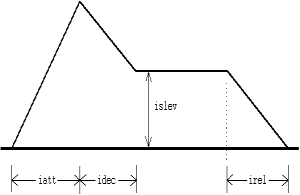
\includegraphics[scale=1]{adsr} 


 Picture of an ADSR envelope.


  The length of the sustain is calculated from the length of the note. This means \emph{adsr}
 is not suitable for use with MIDI events. The opcode \emph{madsr}
 uses the \emph{linsegr}
 mechanism, and so can be used in MIDI applications. 
\subsection*{Examples}


  Here is an example of the madsr opcode. It uses the files \emph{madsr.orc}
 and \emph{madsr.sco}
. 


 \textbf{Example 1. Example of the madsr opcode.}

\begin{lstlisting}
/* madsr.orc */
/* Written by Iain McCurdy */
; Initialize the global variables.
sr = 44100
kr = 441
ksmps = 100
nchnls = 1

; Instrument #1.
instr 1
  ; Attack time.
  iattack = 0.5
  ; Decay time.
  idecay = 0
  ; Sustain level.
  isustain = 1
  ; Release time.
  irelease = 0.5
  aenv madsr iattack, idecay, isustain, irelease

  a1 oscili 10000, 440, 1
  out a1*aenv
endin
/* madsr.orc */
        
\end{lstlisting}
\begin{lstlisting}
/* madsr.sco */
/* Written by Iain McCurdy */
; Table #1, a sine wave.
f 1 0 1024 10 1

; Leave the score running for 6 seconds.
f 0 6

; Play Instrument #1 for two seconds.
i 1 0 2
e
/* madsr.sco */
        
\end{lstlisting}
\subsection*{See Also}


 \emph{adsr}
, \emph{mxadsr}
, \emph{xadsr}

\subsection*{Credits}


 November 2002. Thanks to Rasmus Ekman, added documentation for the \emph{ireltim}
 parameter.


 December 2002. Thanks to Iain McCurdy, added an example.


 December 2002. Thanks to Istvan Varga, added documentation about the maximum release time.


 New in Csound version 3.49.
%\hline 


\begin{comment}
\begin{tabular}{lcr}
Previous &Home &Next \\
maca &Up &mandol

\end{tabular}


\end{document}
\end{comment}

\newpage
\begin{comment}
\documentclass[10pt]{article}
\usepackage{fullpage, graphicx, url}
\setlength{\parskip}{1ex}
\setlength{\parindent}{0ex}
\title{mandol}
\begin{document}


\begin{tabular}{ccc}
The Alternative Csound Reference Manual & & \\
Previous & &Next

\end{tabular}

%\hline 
\end{comment}
\section{mandol}
mandol�--� An emulation of a mandolin. \subsection*{Description}


  An emulation of a mandolin. 
\subsection*{Syntax}


 ar \textbf{mandol}
 kamp, kfreq, kpluck, kdetune, kgain, ksize, ifn [, iminfreq]
\subsection*{Initialization}


 \emph{ifn}
 -- table number containing the pluck wave form. The file \emph{mandpluk.aiff}
 is suitable for this. It is also available at \emph{\url{ftp://ftp.cs.bath.ac.uk/pub/dream/documentation/sounds/modelling/}}
. 


 \emph{iminfreq}
 (optional, default=0) -- Lowest frequency to be played on the note. If it is omitted it is taken to be the same as the initial \emph{kfreq}
. 
\subsection*{Performance}


 \emph{kamp}
 -- Amplitude of note. 


 \emph{kfreq}
 -- Frequency of note played. 


 \emph{kpluck}
 -- The pluck position, in range 0 to 1. Suggest 0.4. 


 \emph{kdetune }
 -- The proportional detuning between the two strings. Suggested range 0.9 to 1. 


 \emph{kgain}
 -- the loop gain of the model, in the range 0.97 to 1. 


 \emph{ksize}
 -- The size of the body of the mandolin. Range 0 to 2. 
\subsection*{Examples}


  Here is an example of the mandol opcode. It uses the files \emph{mandol.orc}
, \emph{mandol.sco}
, and \emph{mandpluk.aiff}
. 


 \textbf{Example 1. Example of the mandol opcode.}

\begin{lstlisting}
/* mandol.orc */
; Initialize the global variables.
sr = 22050
kr = 2205
ksmps = 10
nchnls = 1

; Instrument #1.
instr 1
  ; kamp = 30000
  ; kfreq = 880
  ; kpluck = 0.4
  ; kdetune = 0.99
  ; kgain = 0.99
  ; ksize = 2
  ; ifn = 1
  ; ifreq = 220

  a1 mandol 30000, 880, 0.4, 0.99, 0.99, 2, 1, 220

  out a1
endin
/* mandol.orc */
        
\end{lstlisting}
\begin{lstlisting}
/* mandol.sco */
; Table #1: the "mandpluk.aiff" audio file
f 1 0 8192 1 "mandpluk.aiff" 0 0 0

; Play Instrument #1 for one second.
i 1 0 1
e
/* mandol.sco */
        
\end{lstlisting}
\subsection*{Credits}


 


 


\begin{tabular}{ccc}
Author: John ffitch (after Perry Cook) &University of Bath, Codemist Ltd. &Bath, UK

\end{tabular}



 


 Example written by Kevin Conder.


 New in Csound version 3.47
%\hline 


\begin{comment}
\begin{tabular}{lcr}
Previous &Home &Next \\
madsr &Up &marimba

\end{tabular}


\end{document}
\end{comment}

\newpage
\begin{comment}
\documentclass[10pt]{article}
\usepackage{fullpage, graphicx, url}
\setlength{\parskip}{1ex}
\setlength{\parindent}{0ex}
\title{marimba}
\begin{document}


\begin{tabular}{ccc}
The Alternative Csound Reference Manual & & \\
Previous & &Next

\end{tabular}

%\hline 
\end{comment}
\section{marimba}
marimba�--� Physical model related to the striking of a wooden block. \subsection*{Description}


  Audio output is a tone related to the striking of a wooden block as found in a marimba. The method is a physical model developed from Perry Cook but re-coded for Csound. 
\subsection*{Syntax}


 ar \textbf{marimba}
 kamp, kfreq, ihrd, ipos, imp, kvibf, kvamp, ivibfn, idec [, idoubles] [, itriples]
\subsection*{Initialization}


 \emph{ihrd}
 -- the hardness of the stick used in the strike. A range of 0 to 1 is used. 0.5 is a suitable value. 


 \emph{ipos}
 -- where the block is hit, in the range 0 to 1. 


 \emph{imp}
 -- a table of the strike impulses. The file \emph{marmstk1.wav}
 is a suitable function from measurements and can be loaded with a \emph{GEN01}
 table. It is also available at \emph{\url{ftp://ftp.cs.bath.ac.uk/pub/dream/documentation/sounds/modelling/}}
. 


 \emph{ivfn}
 -- shape of vibrato, usually a sine table, created by a function 


 \emph{idec}
 -- time before end of note when damping is introduced 


 \emph{idoubles}
 (optional) -- percentage of double strikes. Default is 40\%. 


 \emph{itriples}
 (optional) -- percentage of triple strikes. Default is 20\%. 
\subsection*{Performance}


 \emph{kamp}
 -- Amplitude of note. 


 \emph{kfreq}
 -- Frequency of note played. 


 \emph{kvibf}
 -- frequency of vibrato in Hertz. Suggested range is 0 to 12 


 \emph{kvamp}
 -- amplitude of the vibrato 
\subsection*{Examples}


  Here is an example of the marimba opcode. It uses the files \emph{marimba.orc}
, \emph{marimba.sco}
, and \emph{marmstk1.wav}
. 


 \textbf{Example 1. Example of the marimba opcode.}

\begin{lstlisting}
/* marimba.orc */
; Initialize the global variables.
sr = 22050
kr = 2205
ksmps = 10
nchnls = 1

; Instrument #1.
instr 1
  ; kamp = 31129.60
  ; kfreq = 440
  ; ihrd = 0.5
  ; ipos = 0.561
  ; imp = 1
  ; kvibf = 6.0
  ; kvamp = 0.05
  ; ivibfn = 2
  ; idec = 0.1

  a1 marimba 31129.60, 440, 0.5, 0.561, 1, 6.0, 0.05, 2, 0.1

  out a1
endin
/* marimba.orc */
        
\end{lstlisting}
\begin{lstlisting}
/* marimba.sco */
; Table #1, the "marmstk1.wav" audio file.
f 1 0 256 1 "marmstk1.wav" 0 0 0
; Table #2, a sine wave for the vibrato.
f 2 0 128 10 1

; Play Instrument #1 for one second.
i 1 0 1
e
/* marimba.sco */
        
\end{lstlisting}
\subsection*{See Also}


 \emph{vibes}

\subsection*{Credits}


 


 


\begin{tabular}{ccc}
Author: John ffitch (after Perry Cook) &University of Bath, Codemist Ltd. &Bath, UK

\end{tabular}



 


 New in Csound version 3.47
%\hline 


\begin{comment}
\begin{tabular}{lcr}
Previous &Home &Next \\
mandol &Up &massign

\end{tabular}


\end{document}
\end{comment}

\newpage
\begin{comment}
\documentclass[10pt]{article}
\usepackage{fullpage, graphicx, url}
\setlength{\parskip}{1ex}
\setlength{\parindent}{0ex}
\title{massign}
\begin{document}


\begin{tabular}{ccc}
The Alternative Csound Reference Manual & & \\
Previous & &Next

\end{tabular}

%\hline 
\end{comment}
\section{massign}
massign�--� Assigns a MIDI channel number to a Csound instrument. \subsection*{Description}


  Assigns a MIDI channel number to a Csound instrument. 
\subsection*{Syntax}


 \textbf{massign}
 ichnl, insnum


 \textbf{massign}
 ichnl, ``insname''
\subsection*{Initialization}


 \emph{ichnl}
 -- MIDI channel number (1-16) 


 \emph{insnum}
 -- Csound orchestra instrument number 


 \emph{``insname''}
 -- A string (in double-quotes) representing a named instrument. 
\subsection*{Performance}


  Assigns a MIDI channel number to a Csound instrument. 
\subsection*{See Also}


 \emph{ctrlinit}

\subsection*{Credits}


 


 


\begin{tabular}{cc}
Author: Barry L. Vercoe - Mike Berry &MIT, Cambridge, Mass.

\end{tabular}



 


 New in Csound version 3.47


 Thanks goes to Rasmus Ekman for pointing out the correct MIDI channel and controller number ranges.
%\hline 


\begin{comment}
\begin{tabular}{lcr}
Previous &Home &Next \\
marimba &Up &maxalloc

\end{tabular}


\end{document}
\end{comment}

\newpage
%\begin{comment}
\documentclass[10pt]{article}
\usepackage{fullpage, graphicx, url}
\setlength{\parskip}{1ex}
\setlength{\parindent}{0ex}
\title{Arithmetic and Logic Operations}
\begin{document}


\begin{tabular}{ccc}
The Alternative Csound Reference Manual & & \\
Previous &Mathematical Operations &Next

\end{tabular}

%\hline 
\end{comment}
\section{Arithmetic and Logic Operations}


  Opcodes that perform arithmetic and logic operations are \emph{-}
, \emph{+}
, \emph{\&\&}
, \emph{||}
, \emph{*}
, \emph{/}
, \emph{\^{}}
, and \emph{\%}
. 
%\hline 


\begin{comment}
\begin{tabular}{lcr}
Previous &Home &Next \\
Mathematical Operations &Up &Mathematical Functions

\end{tabular}


\end{document}
\end{comment}

%\begin{comment}
\documentclass[10pt]{article}
\usepackage{fullpage, graphicx, url}
\setlength{\parskip}{1ex}
\setlength{\parindent}{0ex}
\title{Mathematical Functions}
\begin{document}


\begin{tabular}{ccc}
The Alternative Csound Reference Manual & & \\
Previous &Mathematical Operations &Next

\end{tabular}

%\hline 
\end{comment}
\section{Mathematical Functions}


  Opcodes that perform mathematical functions are \emph{abs}
, \emph{exp}
, \emph{frac}
, \emph{int}
, \emph{log}
, \emph{log10}
, \emph{logbtwo}
, \emph{powoftwo}
, and \emph{sqrt}
. 
%\hline 


\begin{comment}
\begin{tabular}{lcr}
Previous &Home &Next \\
Arithmetic and Logic Operations &Up &Opcode Equivalents of Functions

\end{tabular}


\end{document}
\end{comment}

%\begin{comment}
\documentclass[10pt]{article}
\usepackage{fullpage, graphicx, url}
\setlength{\parskip}{1ex}
\setlength{\parindent}{0ex}
\title{Opcode Equivalents of Functions}
\begin{document}


\begin{tabular}{ccc}
The Alternative Csound Reference Manual & & \\
Previous &Mathematical Operations &Next

\end{tabular}

%\hline 
\end{comment}
\section{Opcode Equivalents of Functions}


  Opcodes that perform the equivalent of mathematical functions are \emph{mac}
, \emph{maca}
, \emph{pow}
, \emph{product}
, and \emph{sum}
. 
%\hline 


\begin{comment}
\begin{tabular}{lcr}
Previous &Home &Next \\
Mathematical Functions &Up &Random Functions

\end{tabular}


\end{document}
\end{comment}

%\begin{comment}
\documentclass[10pt]{article}
\usepackage{fullpage, graphicx, url}
\setlength{\parskip}{1ex}
\setlength{\parindent}{0ex}
\title{Random Functions}
\begin{document}


\begin{tabular}{ccc}
The Alternative Csound Reference Manual & & \\
Previous &Mathematical Operations &Next

\end{tabular}

%\hline 
\end{comment}
\section{Random Functions}


  Opcodes that perform random functions are \emph{birnd}
 and \emph{rnd}
. 
%\hline 


\begin{comment}
\begin{tabular}{lcr}
Previous &Home &Next \\
Opcode Equivalents of Functions &Up &Trigonometric Functions

\end{tabular}


\end{document}
\end{comment}

%\begin{comment}
\documentclass[10pt]{article}
\usepackage{fullpage, graphicx, url}
\setlength{\parskip}{1ex}
\setlength{\parindent}{0ex}
\title{Mathematical Operations}
\begin{document}


\begin{tabular}{ccc}
The Alternative Csound Reference Manual & & \\
Previous & &Next

\end{tabular}

%\hline 
\end{comment}
\section{Mathematical Operations}
\section{Amplitude Converters}


  Opcodes to convert between different amplitude measurements are \emph{ampdb}
, \emph{ampdbfs}
, \emph{dbamp}
, and \emph{dbfsamp}
. 
%\hline 


\begin{comment}
\begin{tabular}{lcr}
Previous &Home &Next \\
Table Selection &Up &Arithmetic and Logic Operations

\end{tabular}


\end{document}
\end{comment}

%\begin{comment}
\documentclass[10pt]{article}
\usepackage{fullpage, graphicx, url}
\setlength{\parskip}{1ex}
\setlength{\parindent}{0ex}
\title{Trigonometric Functions}
\begin{document}


\begin{tabular}{ccc}
The Alternative Csound Reference Manual & & \\
Previous &Mathematical Operations &Next

\end{tabular}

%\hline 
\end{comment}
\section{Trigonometric Functions}


  Opcodes that perform trigonometric functions are \emph{cos}
, \emph{cosh}
, \emph{cosinv}
, \emph{sin}
, \emph{sinh}
, \emph{sininv}
, \emph{tan}
, \emph{tanh}
, \emph{taninv}
, and \emph{taninv2}
. 
%\hline 


\begin{comment}
\begin{tabular}{lcr}
Previous &Home &Next \\
Random Functions &Up &MIDI Support

\end{tabular}


\end{document}
\end{comment}

\begin{comment}
\documentclass[10pt]{article}
\usepackage{fullpage, graphicx, url}
\setlength{\parskip}{1ex}
\setlength{\parindent}{0ex}
\title{maxalloc}
\begin{document}


\begin{tabular}{ccc}
The Alternative Csound Reference Manual & & \\
Previous & &Next

\end{tabular}

%\hline 
\end{comment}
\section{maxalloc}
maxalloc�--� Limits the number of allocations of an instrument. \subsection*{Description}


  Limits the number of allocations of an instrument. 
\subsection*{Syntax}


 \textbf{maxalloc}
 insnum, icount
\subsection*{Initialization}


 \emph{insnum}
 -- instrument number 


 \emph{icount}
 -- number of instrument allocations 
\subsection*{Performance}


  All instances of \emph{maxalloc}
 must be defined in the header section, not in the instrument body. 
\subsection*{Examples}


  Here is an example of the maxalloc opcode. It uses the files \emph{maxalloc.orc}
 and \emph{maxalloc.sco}
. 


 \textbf{Example 1. Example of the maxalloc opcode.}

\begin{lstlisting}
/* maxalloc.orc */
; Initialize the global variables.
sr = 44100
kr = 4410
ksmps = 10
nchnls = 1

; Limit Instrument #1 to three instances.
maxalloc 1, 3
 
; Instrument #1
instr 1
  ; Generate a waveform, get the cycles per second from the 4th p-field.
  a1 oscil 6500, p4, 1
  out a1
endin
/* maxalloc.orc */
        
\end{lstlisting}
\begin{lstlisting}
/* maxalloc.sco */
; Just generate a nice, ordinary sine wave.
f 1 0 32768 10 1

; Play five instances of Instrument #1 for one second.
; Note that 4th p-field contains cycles per second.
i 1 0 1 220
i 1 0 1 440
i 1 0 1 880
i 1 0 1 1320
i 1 0 1 1760
e
/* maxalloc.sco */
        
\end{lstlisting}
 Its output should contain a message like this: \begin{lstlisting}
WARNING: cannot allocate last note because it exceeds instr maxalloc
      
\end{lstlisting}
\subsection*{See Also}


 \emph{cpuprc}
, \emph{prealloc}

\subsection*{Credits}


 


 


\begin{tabular}{ccc}
Author: Gabriel Maldonado &Italy &July 1999

\end{tabular}



 


 Example written by Kevin Conder.


 New in Csound version 3.57
%\hline 


\begin{comment}
\begin{tabular}{lcr}
Previous &Home &Next \\
massign &Up &mclock

\end{tabular}


\end{document}
\end{comment}

\newpage
\begin{comment}
\documentclass[10pt]{article}
\usepackage{fullpage, graphicx, url}
\setlength{\parskip}{1ex}
\setlength{\parindent}{0ex}
\title{mclock}
\begin{document}


\begin{tabular}{ccc}
The Alternative Csound Reference Manual & & \\
Previous & &Next

\end{tabular}

%\hline 
\end{comment}
\section{mclock}
mclock�--� Sends a MIDI CLOCK message. \subsection*{Description}


  Sends a MIDI CLOCK message. 
\subsection*{Syntax}


 \textbf{mclock}
 ifreq
\subsection*{Initialization}


 \emph{ifreq}
 -- clock message frequency rate in Hz 
\subsection*{Performance}


  Sends a MIDI CLOCK message (0xF8) every 1/\emph{ifreq}
 seconds. So \emph{ifreq}
 is the frequency rate of CLOCK message in Hz. 
\subsection*{See Also}


 \emph{mrtmsg}

\subsection*{Credits}


 


 


\begin{tabular}{cc}
Author: Gabriel Maldonado &Italy

\end{tabular}



 


 New in Csound version 3.47
%\hline 


\begin{comment}
\begin{tabular}{lcr}
Previous &Home &Next \\
maxalloc &Up &mdelay

\end{tabular}


\end{document}
\end{comment}

\newpage
\begin{comment}
\documentclass[10pt]{article}
\usepackage{fullpage, graphicx, url}
\setlength{\parskip}{1ex}
\setlength{\parindent}{0ex}
\title{mdelay}
\begin{document}


\begin{tabular}{ccc}
The Alternative Csound Reference Manual & & \\
Previous & &Next

\end{tabular}

%\hline 
\end{comment}
\section{mdelay}
mdelay�--� A MIDI delay opcode. \subsection*{Description}


  A MIDI delay opcode. 
\subsection*{Syntax}


 \textbf{mdelay}
 kstatus, kchan, kd1, kd2, kdelay
\subsection*{Performance}


 \emph{kstatus}
 -- status byte of MIDI message to be delayed 


 \emph{kchan}
 -- MIDI channel (1-16) 


 \emph{kd1}
 -- first MIDI data byte 


 \emph{kd2}
 -- second MIDI data byte 


 \emph{kdelay}
 -- delay time in seconds 


  Each time that \emph{kstatus}
 is other than zero, \emph{mdelay}
 outputs a MIDI message to the MIDI out port after \emph{kdelay}
 seconds. This opcode is useful in implementing MIDI delays. Several instances of \emph{mdelay}
 can be present in the same instrument with different argument values, so complex and colorful MIDI echoes can be implemented. Further, the delay time can be changed at k-rate. 
\subsection*{Credits}


 


 


\begin{tabular}{ccc}
Author: Gabriel Maldonado &Italy &November 1998

\end{tabular}



 


 New in Csound version 3.492
%\hline 


\begin{comment}
\begin{tabular}{lcr}
Previous &Home &Next \\
mclock &Up &midic14

\end{tabular}


\end{document}
\end{comment}

\newpage
\begin{comment}
\documentclass[10pt]{article}
\usepackage{fullpage, graphicx, url}
\setlength{\parskip}{1ex}
\setlength{\parindent}{0ex}
\title{midic14}
\begin{document}


\begin{tabular}{ccc}
The Alternative Csound Reference Manual & & \\
Previous & &Next

\end{tabular}

%\hline 
\end{comment}
\section{midic14}
midic14�--� Allows a floating-point 14-bit MIDI signal scaled with a minimum and a maximum range. \subsection*{Description}


  Allows a floating-point 14-bit MIDI signal scaled with a minimum and a maximum range. 
\subsection*{Syntax}


 idest \textbf{midic14}
 ictlno1, ictlno2, imin, imax [, ifn]


 kdest \textbf{midic14}
 ictlno1, ictlno2, kmin, kmax [, ifn]
\subsection*{Initialization}


 \emph{idest}
 -- output signal 


 \emph{ictln1o}
 -- most-significant byte controller number (0-127) 


 \emph{ictlno2}
 -- least-significant byte controller number (0-127) 


 \emph{imin}
 -- user-defined minimum floating-point value of output 


 \emph{imax}
 -- user-defined maximum floating-point value of output 


 \emph{ifn}
 (optional) -- table to be read when indexing is required. Table must be normalized. Output is scaled according to \emph{imin}
 and \emph{imax}
 values. 
\subsection*{Performance}


 \emph{kdest}
 -- output signal 


 \emph{kmin}
 -- user-defined minimum floating-point value of output 


 \emph{kmax}
 -- user-defined maximum floating-point value of output 


 \emph{midic14}
 (i- and k-rate 14 bit MIDI control) allows a floating-point 14-bit MIDI signal scaled with a minimum and a maximum range. The minimum and maximum values can be varied at k-rate. It can use optional interpolated table indexing. It requires two MIDI controllers as input. 
\subsection*{See Also}


 \emph{ctrl7}
, \emph{ctrl14}
, \emph{ctrl21}
, \emph{initc7}
, \emph{initc14}
, \emph{initc21}
, \emph{midic7}
, \emph{midic21}

\subsection*{Credits}


 


 


\begin{tabular}{cc}
Author: Gabriel Maldonado &Italy

\end{tabular}



 


 New in Csound version 3.47


 Thanks goes to Rasmus Ekman for pointing out the correct MIDI channel and controller number ranges.
%\hline 


\begin{comment}
\begin{tabular}{lcr}
Previous &Home &Next \\
mdelay &Up &midic21

\end{tabular}


\end{document}
\end{comment}

\newpage
\begin{comment}
\documentclass[10pt]{article}
\usepackage{fullpage, graphicx, url}
\setlength{\parskip}{1ex}
\setlength{\parindent}{0ex}
\title{midic21}
\begin{document}


\begin{tabular}{ccc}
The Alternative Csound Reference Manual & & \\
Previous & &Next

\end{tabular}

%\hline 
\end{comment}
\section{midic21}
midic21�--� Allows a floating-point 21-bit MIDI signal scaled with a minimum and a maximum range. \subsection*{Description}


  Allows a floating-point 21-bit MIDI signal scaled with a minimum and a maximum range. 
\subsection*{Syntax}


 idest \textbf{midic21}
 ictlno1, ictlno2, ictlno3, imin, imax [, ifn]


 kdest \textbf{midic21}
 ictlno1, ictlno2, ictlno3, kmin, kmax [, ifn]
\subsection*{Initialization}


 \emph{idest}
 -- output signal 


 \emph{ictln1o}
 -- most-significant byte controller number (0-127) 


 \emph{ictlno2}
 -- mid-significant byte controller number (0-127) 


 \emph{ictlno3}
 -- least-significant byte controller number (0-127) 


 \emph{imin}
 -- user-defined minimum floating-point value of output 


 \emph{imax}
 -- user-defined maximum floating-point value of output 


 \emph{ifn}
 (optional) -- table to be read when indexing is required. Table must be normalized. Output is scaled according to the \emph{imin}
 and \emph{imax}
 values. 
\subsection*{Performance}


 \emph{kdest}
 -- output signal 


 \emph{kmin}
 -- user-defined minimum floating-point value of output 


 \emph{kmax}
 -- user-defined maximum floating-point value of output 


 \emph{midic21}
 (i- and k-rate 21 bit MIDI control) allows a floating-point 21-bit MIDI signal scaled with a minimum and a maximum range. Minimum and maximum values can be varied at k-rate. It can use optional interpolated table indexing. It requires three MIDI controllers as input. 
\subsection*{See Also}


 \emph{ctrl7}
, \emph{ctrl14}
, \emph{ctrl21}
, \emph{initc7}
, \emph{initc14}
, \emph{initc21}
, \emph{midic7}
, \emph{midic14}

\subsection*{Credits}


 


 


\begin{tabular}{cc}
Author: Gabriel Maldonado &Italy

\end{tabular}



 


 New in Csound version 3.47


 Thanks goes to Rasmus Ekman for pointing out the correct MIDI channel and controller number ranges.
%\hline 


\begin{comment}
\begin{tabular}{lcr}
Previous &Home &Next \\
midic14 &Up &midic7

\end{tabular}


\end{document}
\end{comment}

\newpage
\begin{comment}
\documentclass[10pt]{article}
\usepackage{fullpage, graphicx, url}
\setlength{\parskip}{1ex}
\setlength{\parindent}{0ex}
\title{midic7}
\begin{document}


\begin{tabular}{ccc}
The Alternative Csound Reference Manual & & \\
Previous & &Next

\end{tabular}

%\hline 
\end{comment}
\section{midic7}
midic7�--� Allows a floating-point 7-bit MIDI signal scaled with a minimum and a maximum range. \subsection*{Description}


  Allows a floating-point 7-bit MIDI signal scaled with a minimum and a maximum range. 
\subsection*{Syntax}


 idest \textbf{midic7}
 ictlno, imin, imax [, ifn]


 kdest \textbf{midic7}
 ictlno, kmin, kmax [, ifn]
\subsection*{Initialization}


 \emph{idest}
 -- output signal 


 \emph{ictlno}
 -- MIDI controller number (0-127) 


 \emph{imin}
 -- user-defined minimum floating-point value of output 


 \emph{imax}
 -- user-defined maximum floating-point value of output 


 \emph{ifn}
 (optional) -- table to be read when indexing is required. Table must be normalized. Output is scaled according to the \emph{imin}
 and \emph{imax}
 values. 
\subsection*{Performance}


 \emph{kdest}
 -- output signal 


 \emph{kmin}
 -- user-defined minimum floating-point value of output 


 \emph{kmax}
 -- user-defined maximum floating-point value of output 


 \emph{midic7}
 (i- and k-rate 7 bit MIDI control) allows a floating-point 7-bit MIDI signal scaled with a minimum and a maximum range. It also allows optional non-interpolated table indexing. In \emph{midic7}
 minimum and maximum values can be varied at k-rate. 
\subsection*{See Also}


 \emph{ctrl7}
, \emph{ctrl14}
, \emph{ctrl21}
, \emph{initc7}
, \emph{initc14}
, \emph{initc21}
, \emph{midic14}
, \emph{midic21}

\subsection*{Credits}


 


 


\begin{tabular}{cc}
Author: Gabriel Maldonado &Italy

\end{tabular}



 


 New in Csound version 3.47


 Thanks goes to Rasmus Ekman for pointing out the correct MIDI channel and controller number ranges.
%\hline 


\begin{comment}
\begin{tabular}{lcr}
Previous &Home &Next \\
midic21 &Up &midichannelaftertouch

\end{tabular}


\end{document}
\end{comment}

\newpage
\begin{comment}
\documentclass[10pt]{article}
\usepackage{fullpage, graphicx, url}
\setlength{\parskip}{1ex}
\setlength{\parindent}{0ex}
\title{midichannelaftertouch}
\begin{document}


\begin{tabular}{ccc}
The Alternative Csound Reference Manual & & \\
Previous & &Next

\end{tabular}

%\hline 
\end{comment}
\section{midichannelaftertouch}
midichannelaftertouch�--� Gets a MIDI channel's aftertouch value. \subsection*{Description}


 \emph{midichannelaftertouch}
 is designed to simplify writing instruments that can be used interchangeably for either score or MIDI input, and to make it easier to adapt instruments originally written for score input to work with MIDI input. 


  In general, it should be possible to write instrument definitions that work identically with both scores and MIDI, including both MIDI files and real-time MIDI input, without using any conditional statements, and that take full advantage of MIDI voice messages. 


  Note that correlating Csound instruments with MIDI channel numbers is done using the \emph{massign}
 opcode for real-time performance,. For file-driven performance, instrument numbers default to MIDI channel number + 1, but the defaults are overridden by any MIDI program change messages in the file. 
\subsection*{Syntax}


 \textbf{midichannelaftertouch}
 xchannelaftertouch [, ilow] [, ihigh]
\subsection*{Initialization}


 \emph{ilow}
 (optional) -- optional low value after rescaling, defaults to 0. 


 \emph{ihigh}
 (optional) -- optional high value after rescaling, defaults to 127. 
\subsection*{Performance}


 \emph{xchannelaftertouch}
 -- returns the MIDI channel aftertouch during MIDI activation, remains unchanged otherwise. 


  If the instrument was activated by MIDI input, the opcode overwrites the value of \emph{xchannelaftertouch}
 with the corresponding value from MIDI input. If the instrument was \emph{NOT}
 activated by MIDI input, the value of \emph{xchannelaftertouch}
 remains unchanged. 


  This enables score p-fields to receive MIDI input data during MIDI activation, and score values otherwise. 


 


\begin{tabular}{cc}
\textbf{Adapting a score-activated Csound instrument.}
 \\
� &

  To adapt an ordinary Csound instrument designed for score activation for score/MIDI interoperability: 


 
\begin{itemize}
\item 

 Change all \emph{linen}
, \emph{linseg}
, and \emph{expseg}
 opcodes to \emph{linenr}
, \emph{linsegr}
, and \emph{expsegr}
, respectively, except for a de-clicking or damping envelope. This will not materially change score-driven performance.

\item 

 Add the following lines at the beginning of the instrument definition: 


 
\begin{lstlisting}
; Ensures that a MIDI-activated instrument
; will have a positive p3 field.
mididefault 60, p3 
; Puts MIDI key translated to cycles per
; second into p4, and MIDI velocity into p5
midinoteoncps p4, p5 
                
\end{lstlisting}


 


\end{itemize}


\end{tabular}

 Obviously, \emph{midinoteoncps}
 could be changed to \emph{midinoteonoct}
 or any of the other options, and the choice of p-fields is arbitrary. \subsection*{Examples}


  Here is an example of the midichannelaftertouch opcode. It uses the files \emph{midichannelaftertouch.orc}
 and \emph{midichannelaftertouch.sco}
. 


 \textbf{Example 1. Example of the midichannelaftertouch opcode.}

\begin{lstlisting}
/* midichannelaftertouch.orc */
; Initialize the global variables.
sr = 44100
kr = 4410
ksmps = 10
nchnls = 1

; Instrument #1.
instr 1
  kaft init 0
  midichannelaftertouch kaft

  ; Display the aftertouch value when it changes.
  printk2 kaft
endin
/* midichannelaftertouch.orc */
        
\end{lstlisting}
\begin{lstlisting}
/* midichannelaftertouch.sco */
; Play Instrument #1 for ten seconds.
i 1 0 10
e
/* midichannelaftertouch.sco */
        
\end{lstlisting}
 Its output should include lines like: \begin{lstlisting}
 i1   127.00000
 i1    20.00000
 i1    44.00000
      
\end{lstlisting}
\subsection*{See Also}


 \emph{midicontrolchange}
, \emph{mididefault}
, \emph{midinoteoff}
, \emph{midinoteoncps}
, \emph{midinoteonkey}
, \emph{midinoteonoct}
, \emph{midinoteonpch}
, \emph{midipitchbend}
, \emph{midipolyaftertouch}
, \emph{midiprogramchange}

\subsection*{Credits}


 Author: Michael Gogins


 Example written by Kevin Conder.


 New in version 4.20
%\hline 


\begin{comment}
\begin{tabular}{lcr}
Previous &Home &Next \\
midic7 &Up &midichn

\end{tabular}


\end{document}
\end{comment}

\newpage
\begin{comment}
\documentclass[10pt]{article}
\usepackage{fullpage, graphicx, url}
\setlength{\parskip}{1ex}
\setlength{\parindent}{0ex}
\title{midichn}
\begin{document}


\begin{tabular}{ccc}
The Alternative Csound Reference Manual & & \\
Previous & &Next

\end{tabular}

%\hline 
\end{comment}
\section{midichn}
midichn�--� Returns the MIDI channel number from which the note was activated. \subsection*{Description}


 \emph{midichn}
 returns the MIDI channel number (1 - 16) from which the note was activated. In the case of score notes, it returns 0. 
\subsection*{Syntax}


 ichn \textbf{midichn}

\subsection*{Initialization}


 \emph{ichn}
 -- channel number. If the current note was activated from score, it is set to zero. 
\subsection*{Examples}


  Here is a simple example of the midichn opcode. It uses the files \emph{midichn.orc}
 and \emph{midichn.sco}
. 


 \textbf{Example 1. Example of the midichn opcode.}

\begin{lstlisting}
/* midichn.orc */
; Initialize the global variables.
sr = 44100
kr = 4410
ksmps = 10
nchnls = 1

; Instrument #1.
instr 1
  i1 midichn

  print i1
endin
/* midichn.orc */
        
\end{lstlisting}
\begin{lstlisting}
/* midichn.sco */
; Play Instrument #1 for 12 seconds.
i 1 0 12
e
/* midichn.sco */
        
\end{lstlisting}


  Here is an advanced example of the midichn opcode. It uses the files \emph{midichn\_advanced.mid}
, \emph{midichn\_advanced.orc}
, and \emph{midichn\_advanced.sco}
. 


  Don't forget that you must include the \emph{-F flag}
 when using an external MIDI file like ``midichn\_advanced.mid''. 


 


 \textbf{Example 2. An advanced example of the midichn opcode.}

\begin{lstlisting}
/* midichn_advanced.orc - written by Istvan Varga */
sr	=  44100
ksmps	=  10
nchnls	=  1

	massign  1, 1		; all channels use instr 1
	massign  2, 1
	massign  3, 1
	massign  4, 1
	massign  5, 1
	massign  6, 1
	massign  7, 1
	massign  8, 1
	massign  9, 1
	massign 10, 1
	massign 11, 1
	massign 12, 1
	massign 13, 1
	massign 14, 1
	massign 15, 1
	massign 16, 1

gicnt	=  0			; note counter

	instr 1

gicnt	=  gicnt + 1	; update note counter
kcnt	init gicnt	; copy to local variable
ichn	midichn		; get channel number
istime	times		; note-on time

	if (ichn > 0.5) goto l2		; MIDI note
	printks "note %.0f (time = %.2f) was activated from the score\\n", \
		3600, kcnt, istime
	goto l1
l2:
	printks "note %.0f (time = %.2f) was activated from channel %.0f\\n", \
		3600, kcnt, istime, ichn
l1:
	endin
/* midichn_advanced.orc - written by Istvan Varga */
        
\end{lstlisting}
\begin{lstlisting}
/* midichn_advanced.sco - written by Istvan Varga */
t 0 60
f 0 6 2 -2 0
i 1 1 0.5
i 1 4 0.5
e
/* midichn_advanced.sco - written by Istvan Varga */
        
\end{lstlisting}
 Its output should include lines like: \begin{lstlisting}
note 7 (time = 0.00) was activated from channel 4
note 8 (time = 0.00) was activated from channel 2
      
\end{lstlisting}
\subsection*{See Also}


 \emph{pgmassign}

\subsection*{Credits}


 


 


\begin{tabular}{cc}
Author: Istvan Varga &May 2002

\end{tabular}



 


 The simple example was written by Kevin Conder.


 New in version 4.20
%\hline 


\begin{comment}
\begin{tabular}{lcr}
Previous &Home &Next \\
midichannelaftertouch &Up &midicontrolchange

\end{tabular}


\end{document}
\end{comment}

\newpage
\begin{comment}
\documentclass[10pt]{article}
\usepackage{fullpage, graphicx, url}
\setlength{\parskip}{1ex}
\setlength{\parindent}{0ex}
\title{midicontrolchange}
\begin{document}


\begin{tabular}{ccc}
The Alternative Csound Reference Manual & & \\
Previous & &Next

\end{tabular}

%\hline 
\end{comment}
\section{midicontrolchange}
midicontrolchange�--� Gets a MIDI control change value. \subsection*{Description}


 \emph{midicontrolchange}
 is designed to simplify writing instruments that can be used interchangeably for either score or MIDI input, and to make it easier to adapt instruments originally written for score input to work with MIDI input. 


  In general, it should be possible to write instrument definitions that work identically with both scores and MIDI, including both MIDI files and real-time MIDI input, without using any conditional statements, and that take full advantage of MIDI voice messages. 


  Note that correlating Csound instruments with MIDI channel numbers is done using the \emph{massign}
 opcode for real-time performance,. For file-driven performance, instrument numbers default to MIDI channel number + 1, but the defaults are overridden by any MIDI program change messages in the file. 
\subsection*{Syntax}


 \textbf{midicontrolchange}
 xcontroller, xcontrollervalue [, ilow] [, ihigh]
\subsection*{Initialization}


 \emph{ilow}
 (optional) -- optional low value after rescaling, defaults to 0. 


 \emph{ihigh}
 (optional) -- optional high value after rescaling, defaults to 127. 
\subsection*{Performance}


 \emph{xcontroller}
 -- specifies a MIDI controller number (0-127). 


 \emph{xcontrollervalue}
 -- returns the value of the MIDI controller during MIDI activation, remains unchanged otherwise. 


  If the instrument was activated by MIDI input, the opcode overwrites the values of the \emph{xcontroller}
 and \emph{xcontrollervalue}
 with the corresponding values from MIDI input. If the instrument was \emph{NOT}
 activated by MIDI input, the values of \emph{xcontroller}
 and \emph{xcontrollervalue}
 remain unchanged. 


  This enables score p-fields to receive MIDI input data during MIDI activation, and score values otherwise. 


 


\begin{tabular}{cc}
\textbf{Adapting a score-activated Csound instrument.}
 \\
� &

  To adapt an ordinary Csound instrument designed for score activation for score/MIDI interoperability: 


 
\begin{itemize}
\item 

 Change all \emph{linen}
, \emph{linseg}
, and \emph{expseg}
 opcodes to \emph{linenr}
, \emph{linsegr}
, and \emph{expsegr}
, respectively, except for a de-clicking or damping envelope. This will not materially change score-driven performance.

\item 

 Add the following lines at the beginning of the instrument definition: 


 
\begin{lstlisting}
; Ensures that a MIDI-activated instrument
; will have a positive p3 field.
mididefault 60, p3 
; Puts MIDI key translated to cycles per
; second into p4, and MIDI velocity into p5
midinoteoncps p4, p5 
                
\end{lstlisting}


 


\end{itemize}


\end{tabular}

 Obviously, \emph{midinoteoncps}
 could be changed to \emph{midinoteonoct}
 or any of the other options, and the choice of p-fields is arbitrary. \subsection*{See Also}


 \emph{midichannelaftertouch}
, \emph{mididefault}
, \emph{midinoteoff}
, \emph{midinoteoncps}
, \emph{midinoteonkey}
, \emph{midinoteonoct}
, \emph{midinoteonpch}
, \emph{midipitchbend}
, \emph{midipolyaftertouch}
, \emph{midiprogramchange}

\subsection*{Credits}


 Author: Michael Gogins


 New in version 4.20


 Thanks goes to Rasmus Ekman for pointing out the correct MIDI channel and controller number ranges.
%\hline 


\begin{comment}
\begin{tabular}{lcr}
Previous &Home &Next \\
midichn &Up &midictrl

\end{tabular}


\end{document}
\end{comment}

\newpage
%\begin{comment}
\documentclass[10pt]{article}
\usepackage{fullpage, graphicx, url}
\setlength{\parskip}{1ex}
\setlength{\parindent}{0ex}
\title{Converters}
\begin{document}


\begin{tabular}{ccc}
The Alternative Csound Reference Manual & & \\
Previous &MIDI Support &Next

\end{tabular}

%\hline 
\end{comment}
\section{Converters}


  Opcodes that convert MIDI values are \emph{ampmidi}
, \emph{cpsmidi}
, \emph{cpsmidib}
, \emph{cpstmid}
, \emph{midictrl}
, \emph{notnum}
, \emph{octmidi}
, \emph{octmidib}
, \emph{pchbend}
, \emph{pchmidi}
, \emph{pchmidib}
, and \emph{veloc}
. 
%\hline 


\begin{comment}
\begin{tabular}{lcr}
Previous &Home &Next \\
MIDI Support &Up &Event Extenders

\end{tabular}


\end{document}
\end{comment}

\begin{comment}
\documentclass[10pt]{article}
\usepackage{fullpage, graphicx, url}
\setlength{\parskip}{1ex}
\setlength{\parindent}{0ex}
\title{midictrl}
\begin{document}


\begin{tabular}{ccc}
The Alternative Csound Reference Manual & & \\
Previous & &Next

\end{tabular}

%\hline 
\end{comment}
\section{midictrl}
midictrl�--� Get the current value (0-127) of a specified MIDI controller. \subsection*{Description}


  Get the current value (0-127) of a specified MIDI controller. 
\subsection*{Syntax}


 ival \textbf{midictrl}
 inum [, imin] [, imax]


 kval \textbf{midictrl}
 inum [, imin] [, imax]
\subsection*{Initialization}


 \emph{inum}
 -- MIDI controller number (0-127) 


 \emph{imin, imax}
 -- set minimum and maximum limits on values obtained. 
\subsection*{Performance}


  Get the current value (0-127) of a specified MIDI controller. 
\subsection*{See Also}


 \emph{aftouch}
, \emph{ampmidi}
, \emph{cpsmidi}
, \emph{cpsmidib}
, \emph{notnum}
, \emph{octmidi}
, \emph{octmidib}
, \emph{pchbend}
, \emph{pchmidi}
, \emph{pchmidib}
, \emph{veloc}

\subsection*{Credits}


 


 


\begin{tabular}{ccc}
Author: Barry L. Vercoe - Mike Berry &MIT - Mills &May 1997

\end{tabular}



 


 Thanks goes to Rasmus Ekman for pointing out the correct MIDI channel and controller number ranges.
%\hline 


\begin{comment}
\begin{tabular}{lcr}
Previous &Home &Next \\
midicontrolchange &Up &mididefault

\end{tabular}


\end{document}
\end{comment}

\newpage
\begin{comment}
\documentclass[10pt]{article}
\usepackage{fullpage, graphicx, url}
\setlength{\parskip}{1ex}
\setlength{\parindent}{0ex}
\title{mididefault}
\begin{document}


\begin{tabular}{ccc}
The Alternative Csound Reference Manual & & \\
Previous & &Next

\end{tabular}

%\hline 
\end{comment}
\section{mididefault}
mididefault�--� Changes values, depending on MIDI activation. \subsection*{Description}


 \emph{mididefault}
 is designed to simplify writing instruments that can be used interchangeably for either score or MIDI input, and to make it easier to adapt instruments originally written for score input to work with MIDI input. 


  In general, it should be possible to write instrument definitions that work identically with both scores and MIDI, including both MIDI files and real-time MIDI input, without using any conditional statements, and that take full advantage of MIDI voice messages. 


  Note that correlating Csound instruments with MIDI channel numbers is done using the \emph{massign}
 opcode for real-time performance,. For file-driven performance, instrument numbers default to MIDI channel number + 1, but the defaults are overridden by any MIDI program change messages in the file. 
\subsection*{Syntax}


 \textbf{mididefault}
 xdefault, xvalue
\subsection*{Performance}


 \emph{xdefault}
 -- specifies a default value that will be used during MIDI activation. 


 \emph{xvalue}
 -- overwritten by \emph{xdefault}
 during MIDI activation, remains unchanged otherwise. 


  If the instrument was activated by MIDI input, the opcode will overwrite the value of \emph{xvalue}
 with the value of \emph{xdefault}
. If the instrument was \emph{NOT}
 activated by MIDI input, \emph{xvalue}
 will remain unchanged. 


  This enables score pfields to receive a default value during MIDI activation, and score values otherwise. 


 


\begin{tabular}{cc}
\textbf{Adapting a score-activated Csound instrument.}
 \\
� &

  To adapt an ordinary Csound instrument designed for score activation for score/MIDI interoperability: 


 
\begin{itemize}
\item 

 Change all \emph{linen}
, \emph{linseg}
, and \emph{expseg}
 opcodes to \emph{linenr}
, \emph{linsegr}
, and \emph{expsegr}
, respectively, except for a de-clicking or damping envelope. This will not materially change score-driven performance.

\item 

 Add the following lines at the beginning of the instrument definition: 


 
\begin{lstlisting}
; Ensures that a MIDI-activated instrument
; will have a positive p3 field.
mididefault 60, p3 
; Puts MIDI key translated to cycles per
; second into p4, and MIDI velocity into p5
midinoteoncps p4, p5 
                
\end{lstlisting}


 


\end{itemize}


\end{tabular}

 Obviously, \emph{midinoteoncps}
 could be changed to \emph{midinoteonoct}
 or any of the other options, and the choice of p-fields is arbitrary. \subsection*{See Also}


 \emph{midichannelaftertouch}
, \emph{midicontrolchange}
, \emph{midinoteoff}
, \emph{midinoteoncps}
, \emph{midinoteonkey}
, \emph{midinoteonoct}
, \emph{midinoteonpch}
, \emph{midipitchbend}
, \emph{midipolyaftertouch}
, \emph{midiprogramchange}

\subsection*{Credits}


 Author: Michael Gogins


 New in version 4.20
%\hline 


\begin{comment}
\begin{tabular}{lcr}
Previous &Home &Next \\
midictrl &Up &midiin

\end{tabular}


\end{document}
\end{comment}

\newpage
%\begin{comment}
\documentclass[10pt]{article}
\usepackage{fullpage, graphicx, url}
\setlength{\parskip}{1ex}
\setlength{\parindent}{0ex}
\title{Event Extenders}
\begin{document}


\begin{tabular}{ccc}
The Alternative Csound Reference Manual & & \\
Previous &MIDI Support &Next

\end{tabular}

%\hline 
\end{comment}
\section{Event Extenders}


  Opcodes that let one extend the duration of an event are \emph{release}
 and \emph{xtratim}
. 
%\hline 


\begin{comment}
\begin{tabular}{lcr}
Previous &Home &Next \\
Converters &Up &Generic Input and Output

\end{tabular}


\end{document}
\end{comment}

%\begin{comment}
\documentclass[10pt]{article}
\usepackage{fullpage, graphicx, url}
\setlength{\parskip}{1ex}
\setlength{\parindent}{0ex}
\title{Generic Input and Output}
\begin{document}


\begin{tabular}{ccc}
The Alternative Csound Reference Manual & & \\
Previous &MIDI Support &Next

\end{tabular}

%\hline 
\end{comment}
\section{Generic Input and Output}


  Opcodes for generic MIDI input and output are \emph{midiin}
 and \emph{midiout}
. 
%\hline 


\begin{comment}
\begin{tabular}{lcr}
Previous &Home &Next \\
Event Extenders &Up &Note-on/Note-off

\end{tabular}


\end{document}
\end{comment}

\begin{comment}
\documentclass[10pt]{article}
\usepackage{fullpage, graphicx, url}
\setlength{\parskip}{1ex}
\setlength{\parindent}{0ex}
\title{midiin}
\begin{document}


\begin{tabular}{ccc}
The Alternative Csound Reference Manual & & \\
Previous & &Next

\end{tabular}

%\hline 
\end{comment}
\section{midiin}
midiin�--� Returns a generic MIDI message received by the MIDI IN port. \subsection*{Description}


  Returns a generic MIDI message received by the MIDI IN port 
\subsection*{Syntax}


 kstatus, kchan, kdata1, kdata2 \textbf{midiin}

\subsection*{Performance}


 \emph{kstatus}
 -- the type of MIDI message. Can be: 


 
\begin{itemize}
\item 

 128 (note off)

\item 

 144 (note on)

\item 

 160 (polyphonic aftertouch)

\item 

 176 (control change)

\item 

 192 (program change)

\item 

 208 (channel aftertouch)

\item 

 224 (pitch bend

\item 

 0 if no MIDI message are pending in the MIDI IN buffer


\end{itemize}


 \emph{kchan}
 -- MIDI channel (1-16) 


 \emph{kdata1, kdata2}
 -- message-dependent data values 


 \emph{midiin}
 has no input arguments, because it reads at the MIDI in port implicitly. It works at k-rate. Normally (i.e., when no messages are pending) \emph{kstatus}
 is zero, only when MIDI data are present in the MIDI IN buffer, is \emph{kstatus}
 set to the type of the relevant messages. 
\subsection*{Credits}


 


 


\begin{tabular}{ccc}
Author: Gabriel Maldonado &Italy &1998

\end{tabular}



 


 New in Csound version 3.492
%\hline 


\begin{comment}
\begin{tabular}{lcr}
Previous &Home &Next \\
mididefault &Up &midinoteoff

\end{tabular}


\end{document}
\end{comment}

\newpage
\begin{comment}
\documentclass[10pt]{article}
\usepackage{fullpage, graphicx, url}
\setlength{\parskip}{1ex}
\setlength{\parindent}{0ex}
\title{midinoteoff}
\begin{document}


\begin{tabular}{ccc}
The Alternative Csound Reference Manual & & \\
Previous & &Next

\end{tabular}

%\hline 
\end{comment}
\section{midinoteoff}
midinoteoff�--� Gets a MIDI noteoff value. \subsection*{Description}


 \emph{midinoteoff}
 is designed to simplify writing instruments that can be used interchangeably for either score or MIDI input, and to make it easier to adapt instruments originally written for score input to work with MIDI input. 


  In general, it should be possible to write instrument definitions that work identically with both scores and MIDI, including both MIDI files and real-time MIDI input, without using any conditional statements, and that take full advantage of MIDI voice messages. 


  Note that correlating Csound instruments with MIDI channel numbers is done using the \emph{massign}
 opcode for real-time performance,. For file-driven performance, instrument numbers default to MIDI channel number + 1, but the defaults are overridden by any MIDI program change messages in the file. 
\subsection*{Syntax}


 \textbf{midinoteoff}
 xkey, xvelocity
\subsection*{Performance}


 \emph{xkey}
 -- returns MIDI key during MIDI activation, remains unchanged otherwise. 


 \emph{xvelocity}
 -- returns MIDI velocity during MIDI activation, remains unchanged otherwise. 


  If the instrument was activated by MIDI input, the opcode overwrites the values of the \emph{xkey}
 and \emph{xvelocity}
 with the corresponding values from MIDI input. If the instrument was \emph{NOT}
 activated by MIDI input, the values of \emph{xkey}
 and \emph{xvelocity}
 remain unchanged. 


  This enables score p-fields to receive MIDI input data during MIDI activation, and score values otherwise. 


 


\begin{tabular}{cc}
\textbf{Adapting a score-activated Csound instrument.}
 \\
� &

  To adapt an ordinary Csound instrument designed for score activation for score/MIDI interoperability: 


 
\begin{itemize}
\item 

 Change all \emph{linen}
, \emph{linseg}
, and \emph{expseg}
 opcodes to \emph{linenr}
, \emph{linsegr}
, and \emph{expsegr}
, respectively, except for a de-clicking or damping envelope. This will not materially change score-driven performance.

\item 

 Add the following lines at the beginning of the instrument definition: 


 
\begin{lstlisting}
; Ensures that a MIDI-activated instrument
; will have a positive p3 field.
mididefault 60, p3 
; Puts MIDI key translated to cycles per
; second into p4, and MIDI velocity into p5
midinoteoncps p4, p5 
                
\end{lstlisting}


 


\end{itemize}


\end{tabular}

 Obviously, \emph{midinoteoncps}
 could be changed to \emph{midinoteonoct}
 or any of the other options, and the choice of p-fields is arbitrary. \subsection*{Examples}


  Here is an example of the midinoteoff opcode. It uses the files \emph{midinoteoff.orc}
 and \emph{midinoteoff.sco}
. 


 \textbf{Example 1. Example of the midinoteoff opcode.}

\begin{lstlisting}
/* midinoteoff.orc */
; Initialize the global variables.
sr = 44100
kr = 4410
ksmps = 10
nchnls = 1

; Instrument #1.
instr 1
  kkey init 0
  kvelocity init 0

  midinoteoff kkey, kvelocity

  ; Display the key value when it changes.
  printk2 kkey
endin
/* midinoteoff.orc */
        
\end{lstlisting}
\begin{lstlisting}
/* midinoteoff.sco */
; Play Instrument #1 for ten seconds.
i 1 0 10
e
/* midinoteoff.sco */
        
\end{lstlisting}
 Its output should include lines like: \begin{lstlisting}
 i1    60.00000
 i1    76.00000
      
\end{lstlisting}
\subsection*{See Also}


 \emph{midichannelaftertouch}
, \emph{midicontrolchange}
, \emph{mididefault}
, \emph{midinoteoncps}
, \emph{midinoteonkey}
, \emph{midinoteonoct}
, \emph{midinoteonpch}
, \emph{midipitchbend}
, \emph{midipolyaftertouch}
, \emph{midiprogramchange}

\subsection*{Credits}


 Author: Michael Gogins


 Example written by Kevin Conder.


 New in version 4.20
%\hline 


\begin{comment}
\begin{tabular}{lcr}
Previous &Home &Next \\
midiin &Up &midinoteoncps

\end{tabular}


\end{document}
\end{comment}

\newpage
\begin{comment}
\documentclass[10pt]{article}
\usepackage{fullpage, graphicx, url}
\setlength{\parskip}{1ex}
\setlength{\parindent}{0ex}
\title{midinoteoncps}
\begin{document}


\begin{tabular}{ccc}
The Alternative Csound Reference Manual & & \\
Previous & &Next

\end{tabular}

%\hline 
\end{comment}
\section{midinoteoncps}
midinoteoncps�--� Gets a MIDI note number as a cycles-per-second frequency. \subsection*{Description}


 \emph{midinoteoncps}
 is designed to simplify writing instruments that can be used interchangeably for either score or MIDI input, and to make it easier to adapt instruments originally written for score input to work with MIDI input. 


  In general, it should be possible to write instrument definitions that work identically with both scores and MIDI, including both MIDI files and real-time MIDI input, without using any conditional statements, and that take full advantage of MIDI voice messages. 


  Note that correlating Csound instruments with MIDI channel numbers is done using the \emph{massign}
 opcode for real-time performance,. For file-driven performance, instrument numbers default to MIDI channel number + 1, but the defaults are overridden by any MIDI program change messages in the file. 
\subsection*{Syntax}


 \textbf{midinoteoncps}
 xcps, xvelocity
\subsection*{Performance}


 \emph{xcps}
 -- returns MIDI key translated to cycles per second during MIDI activation, remains unchanged otherwise. 


 \emph{xvelocity}
 -- returns MIDI velocity during MIDI activation, remains unchanged otherwise. 


  If the instrument was activated by MIDI input, the opcode overwrites the values of \emph{xcps}
 and \emph{xvelocity}
 with the corresponding values from MIDI input. If the instrument was \emph{NOT}
 activated by MIDI input, the values of \emph{xcps}
 and \emph{xvelocity}
 remain unchanged. 


  This enables score p-fields to receive MIDI input data during MIDI activation, and score values otherwise. 


 


\begin{tabular}{cc}
\textbf{Adapting a score-activated Csound instrument.}
 \\
� &

  To adapt an ordinary Csound instrument designed for score activation for score/MIDI interoperability: 


 
\begin{itemize}
\item 

 Change all \emph{linen}
, \emph{linseg}
, and \emph{expseg}
 opcodes to \emph{linenr}
, \emph{linsegr}
, and \emph{expsegr}
, respectively, except for a de-clicking or damping envelope. This will not materially change score-driven performance.

\item 

 Add the following lines at the beginning of the instrument definition: 


 
\begin{lstlisting}
; Ensures that a MIDI-activated instrument
; will have a positive p3 field.
mididefault 60, p3 
; Puts MIDI key translated to cycles per
; second into p4, and MIDI velocity into p5
midinoteoncps p4, p5 
                
\end{lstlisting}


 


\end{itemize}


\end{tabular}

 Obviously, \emph{midinoteoncps}
 could be changed to \emph{midinoteonoct}
 or any of the other options, and the choice of p-fields is arbitrary. \subsection*{Examples}


  Here is an example of the midinoteoncps opcode. It uses the files \emph{midinoteoncps.orc}
 and \emph{midinoteoncps.sco}
. 


 \textbf{Example 1. Example of the midinoteoncps opcode.}

\begin{lstlisting}
/* midinoteoncps.orc */
; Initialize the global variables.
sr = 44100
kr = 4410
ksmps = 10
nchnls = 1

; Instrument #1.
instr 1
  kcps init 0
  kvelocity init 0

  midinoteoncps kcps, kvelocity

  ; Display the cycles-per-second value when it changes.
  printk2 kcps
endin
/* midinoteoncps.orc */
        
\end{lstlisting}
\begin{lstlisting}
/* midinoteoncps.sco */
; Play Instrument #1 for ten seconds.
i 1 0 10
e
/* midinoteoncps.sco */
        
\end{lstlisting}
 Its output should include lines like: \begin{lstlisting}
 i1   261.62561
 i1   440.00006
      
\end{lstlisting}
\subsection*{See Also}


 \emph{midichannelaftertouch}
, \emph{midicontrolchange}
, \emph{mididefault}
, \emph{midinoteoff}
, \emph{midinoteonkey}
, \emph{midinoteonoct}
, \emph{midinoteonpch}
, \emph{midipitchbend}
, \emph{midipolyaftertouch}
, \emph{midiprogramchange}

\subsection*{Credits}


 Author: Michael Gogins


 Example written by Kevin Conder.


 New in version 4.20
%\hline 


\begin{comment}
\begin{tabular}{lcr}
Previous &Home &Next \\
midinoteoff &Up &midinoteonkey

\end{tabular}


\end{document}
\end{comment}

\newpage
\begin{comment}
\documentclass[10pt]{article}
\usepackage{fullpage, graphicx, url}
\setlength{\parskip}{1ex}
\setlength{\parindent}{0ex}
\title{midinoteonkey}
\begin{document}


\begin{tabular}{ccc}
The Alternative Csound Reference Manual & & \\
Previous & &Next

\end{tabular}

%\hline 
\end{comment}
\section{midinoteonkey}
midinoteonkey�--� Gets a MIDI note number value. \subsection*{Description}


 \emph{midinoteonkey}
 is designed to simplify writing instruments that can be used interchangeably for either score or MIDI input, and to make it easier to adapt instruments originally written for score input to work with MIDI input. 


  In general, it should be possible to write instrument definitions that work identically with both scores and MIDI, including both MIDI files and real-time MIDI input, without using any conditional statements, and that take full advantage of MIDI voice messages. 


  Note that correlating Csound instruments with MIDI channel numbers is done using the \emph{massign}
 opcode for real-time performance,. For file-driven performance, instrument numbers default to MIDI channel number + 1, but the defaults are overridden by any MIDI program change messages in the file. 
\subsection*{Syntax}


 \textbf{midinoteonkey}
 xkey, xvelocity
\subsection*{Performance}


 \emph{xkey}
 -- returns MIDI key during MIDI activation, remains unchanged otherwise. 


 \emph{xvelocity}
 -- returns MIDI velocity during MIDI activation, remains unchanged otherwise. 


  If the instrument was activated by MIDI input, the opcode overwrites the values of \emph{xkey}
 and \emph{xvelocity}
 with the corresponding values from MIDI input. If the instrument was \emph{NOT}
 activated by MIDI input, the values of \emph{xkey}
 and \emph{xvelocity}
 remain unchanged. 


  This enables score p-fields to receive MIDI input data during MIDI activation, and score values otherwise. 


 


\begin{tabular}{cc}
\textbf{Adapting a score-activated Csound instrument.}
 \\
� &

  To adapt an ordinary Csound instrument designed for score activation for score/MIDI interoperability: 


 
\begin{itemize}
\item 

 Change all \emph{linen}
, \emph{linseg}
, and \emph{expseg}
 opcodes to \emph{linenr}
, \emph{linsegr}
, and \emph{expsegr}
, respectively, except for a de-clicking or damping envelope. This will not materially change score-driven performance.

\item 

 Add the following lines at the beginning of the instrument definition: 


 
\begin{lstlisting}
; Ensures that a MIDI-activated instrument
; will have a positive p3 field.
mididefault 60, p3 
; Puts MIDI key translated to cycles per
; second into p4, and MIDI velocity into p5
midinoteoncps p4, p5 
                
\end{lstlisting}


 


\end{itemize}


\end{tabular}

 Obviously, \emph{midinoteoncps}
 could be changed to \emph{midinoteonoct}
 or any of the other options, and the choice of p-fields is arbitrary. \subsection*{Examples}


  Here is an example of the midinoteonkey opcode. It uses the files \emph{midinoteonkey.orc}
 and \emph{midinoteonkey.sco}
. 


 \textbf{Example 1. Example of the midinoteonkey opcode.}

\begin{lstlisting}
/* midinoteonkey.orc */
; Initialize the global variables.
sr = 44100
kr = 4410
ksmps = 10
nchnls = 1

; Instrument #1.
instr 1
  kkey init 0
  kvelocity init 0

  midinoteonkey kkey, kvelocity

  ; Display the key value when it changes.
  printk2 kkey
endin
/* midinoteonkey.orc */
        
\end{lstlisting}
\begin{lstlisting}
/* midinoteonkey.sco */
; Play Instrument #1 for ten seconds.
i 1 0 10
e
/* midinoteonkey.sco */
        
\end{lstlisting}
 Its output should include lines like: \begin{lstlisting}
 i1    60.00000
 i1    69.00000
      
\end{lstlisting}
\subsection*{See Also}


 \emph{midichannelaftertouch}
, \emph{midicontrolchange}
, \emph{mididefault}
, \emph{midinoteoff}
, \emph{midinoteoncps}
, \emph{midinoteonoct}
, \emph{midinoteonpch}
, \emph{midipitchbend}
, \emph{midipolyaftertouch}
, \emph{midiprogramchange}

\subsection*{Credits}


 Author: Michael Gogins


 Example written by Kevin Conder.


 New in version 4.20
%\hline 


\begin{comment}
\begin{tabular}{lcr}
Previous &Home &Next \\
midinoteoncps &Up &midinoteonoct

\end{tabular}


\end{document}
\end{comment}

\newpage
\begin{comment}
\documentclass[10pt]{article}
\usepackage{fullpage, graphicx, url}
\setlength{\parskip}{1ex}
\setlength{\parindent}{0ex}
\title{midinoteonoct}
\begin{document}


\begin{tabular}{ccc}
The Alternative Csound Reference Manual & & \\
Previous & &Next

\end{tabular}

%\hline 
\end{comment}
\section{midinoteonoct}
midinoteonoct�--� Gets a MIDI note number value as octave-point-decimal value. \subsection*{Description}


 \emph{midinoteonoct}
 is designed to simplify writing instruments that can be used interchangeably for either score or MIDI input, and to make it easier to adapt instruments originally written for score input to work with MIDI input. 


  In general, it should be possible to write instrument definitions that work identically with both scores and MIDI, including both MIDI files and real-time MIDI input, without using any conditional statements, and that take full advantage of MIDI voice messages. 


  Note that correlating Csound instruments with MIDI channel numbers is done using the \emph{massign}
 opcode for real-time performance,. For file-driven performance, instrument numbers default to MIDI channel number + 1, but the defaults are overridden by any MIDI program change messages in the file. 
\subsection*{Syntax}


 \textbf{midinoteonoct}
 xoct, xvelocity
\subsection*{Performance}


 \emph{xoct}
 -- returns MIDI key translated to linear octaves during MIDI activation, remains unchanged otherwise. 


 \emph{xvelocity}
 -- returns MIDI velocity during MIDI activation, remains unchanged otherwise. 


  If the instrument was activated by MIDI input, the opcode overwrites the values of \emph{xoct}
 and \emph{xvelocity}
 with the corresponding value from MIDI input. If the instrument was \emph{NOT}
 activated by MIDI input, the values of \emph{xoct}
 and \emph{xvelocity}
 remain unchanged. 


  This enables score p-fields to receive MIDI input data during MIDI activation, and score values otherwise. 


 


\begin{tabular}{cc}
\textbf{Adapting a score-activated Csound instrument.}
 \\
� &

  To adapt an ordinary Csound instrument designed for score activation for score/MIDI interoperability: 


 
\begin{itemize}
\item 

 Change all \emph{linen}
, \emph{linseg}
, and \emph{expseg}
 opcodes to \emph{linenr}
, \emph{linsegr}
, and \emph{expsegr}
, respectively, except for a de-clicking or damping envelope. This will not materially change score-driven performance.

\item 

 Add the following lines at the beginning of the instrument definition: 


 
\begin{lstlisting}
; Ensures that a MIDI-activated instrument
; will have a positive p3 field.
mididefault 60, p3 
; Puts MIDI key translated to cycles per
; second into p4, and MIDI velocity into p5
midinoteoncps p4, p5 
                
\end{lstlisting}


 


\end{itemize}


\end{tabular}

 Obviously, \emph{midinoteoncps}
 could be changed to \emph{midinoteonoct}
 or any of the other options, and the choice of p-fields is arbitrary. \subsection*{Examples}


  Here is an example of the midinoteonoct opcode. It uses the files \emph{midinoteonoct.orc}
 and \emph{midinoteonoct.sco}
. 


 \textbf{Example 1. Example of the midinoteonoct opcode.}

\begin{lstlisting}
/* midinoteonoct.orc */
; Initialize the global variables.
sr = 44100
kr = 4410
ksmps = 10
nchnls = 1

; Instrument #1.
instr 1
  koct init 0
  kvelocity init 0

  midinoteonoct koct, kvelocity

  ; Display the octave-point-decimal value when it changes.
  printk2 koct
endin
/* midinoteonoct.orc */
        
\end{lstlisting}
\begin{lstlisting}
/* midinoteonoct.sco */
; Play Instrument #1 for ten seconds.
i 1 0 10
e
/* midinoteonoct.sco */
        
\end{lstlisting}
 Its output should include lines like: \begin{lstlisting}
 i1     8.00000
 i1     9.33333
      
\end{lstlisting}
\subsection*{See Also}


 \emph{midichannelaftertouch}
, \emph{midicontrolchange}
, \emph{mididefault}
, \emph{midinoteoff}
, \emph{midinoteoncps}
, \emph{midinoteonkey}
, \emph{midinoteonpch}
, \emph{midipitchbend}
, \emph{midipolyaftertouch}
, \emph{midiprogramchange}

\subsection*{Credits}


 Author: Michael Gogins


 Example written by Kevin Conder.


 New in version 4.20
%\hline 


\begin{comment}
\begin{tabular}{lcr}
Previous &Home &Next \\
midinoteonkey &Up &midinoteonpch

\end{tabular}


\end{document}
\end{comment}

\newpage
\begin{comment}
\documentclass[10pt]{article}
\usepackage{fullpage, graphicx, url}
\setlength{\parskip}{1ex}
\setlength{\parindent}{0ex}
\title{midinoteonpch}
\begin{document}


\begin{tabular}{ccc}
The Alternative Csound Reference Manual & & \\
Previous & &Next

\end{tabular}

%\hline 
\end{comment}
\section{midinoteonpch}
midinoteonpch�--� Gets a MIDI note number as a pitch-class value. \subsection*{Description}


 \emph{midinoteonpch}
 is designed to simplify writing instruments that can be used interchangeably for either score or MIDI input, and to make it easier to adapt instruments originally written for score input to work with MIDI input. 


  In general, it should be possible to write instrument definitions that work identically with both scores and MIDI, including both MIDI files and real-time MIDI input, without using any conditional statements, and that take full advantage of MIDI voice messages. 


  Note that correlating Csound instruments with MIDI channel numbers is done using the \emph{massign}
 opcode for real-time performance,. For file-driven performance, instrument numbers default to MIDI channel number + 1, but the defaults are overridden by any MIDI program change messages in the file. 
\subsection*{Syntax}


 \textbf{midinoteonpch}
 xpch, xvelocity
\subsection*{Performance}


 \emph{xpch}
 -- returns MIDI key translated to octave.pch during MIDI activation, remains unchanged otherwise. 


 \emph{xvelocity}
 -- returns MIDI velocity during MIDI activation, remains unchanged otherwise. 


  If the instrument was activated by MIDI input, the opcode overwrites the values of \emph{xpch}
 and \emph{xvelocity}
 with the corresponding value from MIDI input. If the instrument was \emph{NOT}
 activated by MIDI input, the values of \emph{xpch}
 and \emph{xvelocity}
 remain unchanged. 


  This enables score p-fields to receive MIDI input data during MIDI activation, and score values otherwise. 


 


\begin{tabular}{cc}
\textbf{Adapting a score-activated Csound instrument.}
 \\
� &

  To adapt an ordinary Csound instrument designed for score activation for score/MIDI interoperability: 


 
\begin{itemize}
\item 

 Change all \emph{linen}
, \emph{linseg}
, and \emph{expseg}
 opcodes to \emph{linenr}
, \emph{linsegr}
, and \emph{expsegr}
, respectively, except for a de-clicking or damping envelope. This will not materially change score-driven performance.

\item 

 Add the following lines at the beginning of the instrument definition: 


 
\begin{lstlisting}
; Ensures that a MIDI-activated instrument
; will have a positive p3 field.
mididefault 60, p3 
; Puts MIDI key translated to cycles per
; second into p4, and MIDI velocity into p5
midinoteoncps p4, p5 
                
\end{lstlisting}


 


\end{itemize}


\end{tabular}

 Obviously, \emph{midinoteoncps}
 could be changed to \emph{midinoteonoct}
 or any of the other options, and the choice of p-fields is arbitrary. \subsection*{Examples}


  Here is an example of the midinoteonpch opcode. It uses the files \emph{midinoteonpch.orc}
 and \emph{midinoteonpch.sco}
. 


 \textbf{Example 1. Example of the midinoteonpch opcode.}

\begin{lstlisting}
/* midinoteonpch.orc */
; Initialize the global variables.
sr = 44100
kr = 4410
ksmps = 10
nchnls = 1

; Instrument #1.
instr 1
  kpch init 0
  kvelocity init 0

  midinoteonpch kpch, kvelocity

  ; Display the pitch-class value when it changes.
  printk2 kpch
endin
/* midinoteonpch.orc */
        
\end{lstlisting}
\begin{lstlisting}
/* midinoteonpch.sco */
; Play Instrument #1 for ten seconds.
i 1 0 10
e
/* midinoteonpch.sco */
        
\end{lstlisting}
 Its output should include lines like: \begin{lstlisting}
 i1     8.09000
 i1     9.05000
      
\end{lstlisting}
\subsection*{See Also}


 \emph{midichannelaftertouch}
, \emph{midicontrolchange}
, \emph{mididefault}
, \emph{midinoteoff}
, \emph{midinoteoncps}
, \emph{midinoteonkey}
, \emph{midinoteonoct}
, \emph{midipitchbend}
, \emph{midipolyaftertouch}
, \emph{midiprogramchange}

\subsection*{Credits}


 Author: Michael Gogins


 Example written by Kevin Conder.


 New in version 4.20
%\hline 


\begin{comment}
\begin{tabular}{lcr}
Previous &Home &Next \\
midinoteonoct &Up &midion

\end{tabular}


\end{document}
\end{comment}

\newpage
\begin{comment}
\documentclass[10pt]{article}
\usepackage{fullpage, graphicx, url}
\setlength{\parskip}{1ex}
\setlength{\parindent}{0ex}
\title{midion}
\begin{document}


\begin{tabular}{ccc}
The Alternative Csound Reference Manual & & \\
Previous & &Next

\end{tabular}

%\hline 
\end{comment}
\section{midion}
midion�--� Plays MIDI notes. \subsection*{Description}


  Plays MIDI notes. 
\subsection*{Syntax}


 \textbf{midion}
 kchn, knum, kvel
\subsection*{Performance}


 \emph{kchn}
 -- MIDI channel number (1-16) 


 \emph{knum}
 -- note number (0-127) 


 \emph{kvel}
 -- velocity (0-127) 


 \emph{midion}
 (k-rate note on) plays MIDI notes with current \emph{kchn}
, \emph{knum}
 and \emph{kvel}
. These arguments can be varied at k-rate. Each time the MIDI converted value of any of these arguments changes, last MIDI note played by current instance of \emph{midion}
 is immediately turned off and a new note with the new argument values is activated. This opcode, as well as \emph{moscil}
, can generate very complex melodic textures if controlled by complex k-rate signals. 


  Any number of \emph{midion}
 opcodes can appear in the same Csound instrument, allowing a counterpoint-style polyphony within a single instrument. 
\subsection*{See Also}


 \emph{moscil}

\subsection*{Credits}


 


 


\begin{tabular}{ccc}
Author: Gabriel Maldonado &Italy &May 1997

\end{tabular}



 


 Thanks goes to Rasmus Ekman for pointing out the correct MIDI channel and controller number ranges.
%\hline 


\begin{comment}
\begin{tabular}{lcr}
Previous &Home &Next \\
midinoteonpch &Up &midion2

\end{tabular}


\end{document}
\end{comment}

\newpage
\begin{comment}
\documentclass[10pt]{article}
\usepackage{fullpage, graphicx, url}
\setlength{\parskip}{1ex}
\setlength{\parindent}{0ex}
\title{midion2}
\begin{document}


\begin{tabular}{ccc}
The Alternative Csound Reference Manual & & \\
Previous & &Next

\end{tabular}

%\hline 
\end{comment}
\section{midion2}
midion2�--� Sends noteon and noteoff messages to the MIDI OUT port. \subsection*{Description}


  Sends noteon and noteoff messages to the MIDI OUT port when triggered by a value different than zero. 
\subsection*{Syntax}


 \textbf{midion2}
 kchn, knum, kvel, ktrig
\subsection*{Performance}


 \emph{kchn}
 -- MIDI channel (1-16) 


 \emph{knum}
 -- MIDI note number (0-127) 


 \emph{kvel}
 -- note velocity (0-127) 


 \emph{ktrig}
 -- trigger input signal (normally 0) 


  Similar to \emph{midion}
, this opcode sends noteon and noteoff messages to the MIDI out port, but only when \emph{ktrig}
 is non-zero. This opcode is can work together with the output of the \emph{trigger}
 opcode. 
\subsection*{Credits}


 


 


\begin{tabular}{ccc}
Author: Gabriel Maldonado &Italy &1998

\end{tabular}



 


 New in Csound version 3.492


 Thanks goes to Rasmus Ekman for pointing out the correct MIDI channel and controller number ranges.
%\hline 


\begin{comment}
\begin{tabular}{lcr}
Previous &Home &Next \\
midion &Up &midiout

\end{tabular}


\end{document}
\end{comment}

\newpage
%\begin{comment}
\documentclass[10pt]{article}
\usepackage{fullpage, graphicx, url}
\setlength{\parskip}{1ex}
\setlength{\parindent}{0ex}
\title{Note-on/Note-off}
\begin{document}


\begin{tabular}{ccc}
The Alternative Csound Reference Manual & & \\
Previous &MIDI Support &Next

\end{tabular}

%\hline 
\end{comment}
\section{Note-on/Note-off}


  Opcodes to turn MIDI notes on or off are \emph{midion}
, \emph{midion2}
, \emph{moscil}
, \emph{noteoff}
, \emph{noteon}
, \emph{noteondur}
, and \emph{noteondur2}
. 
%\hline 


\begin{comment}
\begin{tabular}{lcr}
Previous &Home &Next \\
Generic Input and Output &Up &MIDI Message Output

\end{tabular}


\end{document}
\end{comment}

\begin{comment}
\documentclass[10pt]{article}
\usepackage{fullpage, graphicx, url}
\setlength{\parskip}{1ex}
\setlength{\parindent}{0ex}
\title{midiout}
\begin{document}


\begin{tabular}{ccc}
The Alternative Csound Reference Manual & & \\
Previous & &Next

\end{tabular}

%\hline 
\end{comment}
\section{midiout}
midiout�--� Sends a generic MIDI message to the MIDI OUT port. \subsection*{Description}


  Sends a generic MIDI message to the MIDI OUT port. 
\subsection*{Syntax}


 \textbf{midiout}
 kstatus, kchan, kdata1, kdata2
\subsection*{Performance}


 \emph{kstatus}
 -- the type of MIDI message. Can be: 


 
\begin{itemize}
\item 

 128 (note off)

\item 

 144 (note on)

\item 

 160 (polyphonic aftertouch)

\item 

 176 (control change)

\item 

 192 (program change)

\item 

 208 (channel aftertouch)

\item 

 224 (pitch bend)

\item 

 0 when no MIDI messages must be sent to the MIDI OUT port


\end{itemize}


 \emph{kchan}
 -- MIDI channel (1-16) 


 \emph{kdata1, kdata2}
 -- message-dependent data values 


 \emph{midiout}
 has no output arguments, because it sends a message to the MIDI OUT port implicitly. It works at k-rate. It sends a MIDI message only when \emph{kstatus}
 is non-zero. 


 


\begin{tabular}{cc}
Warning &

 \emph{Warning:}
 Normally \emph{kstatus}
 should be set to 0. Only when the user intends to send a MIDI message, can it be set to the corresponding message type number. 


\end{tabular}

\subsection*{Credits}


 


 


\begin{tabular}{ccc}
Author: Gabriel Maldonado &Italy &1998

\end{tabular}



 


 New in Csound version 3.492
%\hline 


\begin{comment}
\begin{tabular}{lcr}
Previous &Home &Next \\
midion2 &Up &midipitchbend

\end{tabular}


\end{document}
\end{comment}

\newpage
%\begin{comment}
\documentclass[10pt]{article}
\usepackage{fullpage, graphicx, url}
\setlength{\parskip}{1ex}
\setlength{\parindent}{0ex}
\title{MIDI Message Output}
\begin{document}


\begin{tabular}{ccc}
The Alternative Csound Reference Manual & & \\
Previous &MIDI Support &Next

\end{tabular}

%\hline 
\end{comment}
\section{MIDI Message Output}


  Opcodes that send MIDI output are \emph{mdelay}
, \emph{nrpn}
, \emph{outiat}
, \emph{outic}
, \emph{outic14}
, \emph{outipat}
, \emph{outipb}
, \emph{outipc}
, \emph{outkat}
, \emph{outkc}
, \emph{outkc14}
, \emph{outkpat}
, \emph{outkpb}
, and \emph{outkpc}
. 
%\hline 


\begin{comment}
\begin{tabular}{lcr}
Previous &Home &Next \\
Note-on/Note-off &Up &Real-time Messages

\end{tabular}


\end{document}
\end{comment}

\begin{comment}
\documentclass[10pt]{article}
\usepackage{fullpage, graphicx, url}
\setlength{\parskip}{1ex}
\setlength{\parindent}{0ex}
\title{midipitchbend}
\begin{document}


\begin{tabular}{ccc}
The Alternative Csound Reference Manual & & \\
Previous & &Next

\end{tabular}

%\hline 
\end{comment}
\section{midipitchbend}
midipitchbend�--� Gets a MIDI pitchbend value. \subsection*{Description}


 \emph{midipitchbend}
 is designed to simplify writing instruments that can be used interchangeably for either score or MIDI input, and to make it easier to adapt instruments originally written for score input to work with MIDI input. 


  In general, it should be possible to write instrument definitions that work identically with both scores and MIDI, including both MIDI files and real-time MIDI input, without using any conditional statements, and that take full advantage of MIDI voice messages. 


  Note that correlating Csound instruments with MIDI channel numbers is done using the \emph{massign}
 opcode for real-time performance,. For file-driven performance, instrument numbers default to MIDI channel number + 1, but the defaults are overridden by any MIDI program change messages in the file. 
\subsection*{Syntax}


 \textbf{midipitchbend}
 xpitchbend [, ilow] [, ihigh]
\subsection*{Initialization}


 \emph{ilow}
 (optional) -- optional low value after rescaling, defaults to 0. 


 \emph{ihigh}
 (optional) -- optional high value after rescaling, defaults to 127. 
\subsection*{Performance}


 \emph{xpitchbend}
 -- returns the MIDI pitch bend during MIDI activation, remains unchanged otherwise. 


  If the instrument was activated by MIDI input, the opcode overwrites the value of \emph{xpitchbend}
 with the corresponding value from MIDI input. If the instrument was \emph{NOT}
 activated by MIDI input, the value of \emph{xpitchbend}
 remains unchanged. 


  This enables score p-fields to receive MIDI input data during MIDI activation, and score values otherwise. 


 


\begin{tabular}{cc}
\textbf{Adapting a score-activated Csound instrument.}
 \\
� &

  To adapt an ordinary Csound instrument designed for score activation for score/MIDI interoperability: 


 
\begin{itemize}
\item 

 Change all \emph{linen}
, \emph{linseg}
, and \emph{expseg}
 opcodes to \emph{linenr}
, \emph{linsegr}
, and \emph{expsegr}
, respectively, except for a de-clicking or damping envelope. This will not materially change score-driven performance.

\item 

 Add the following lines at the beginning of the instrument definition: 


 
\begin{lstlisting}
; Ensures that a MIDI-activated instrument
; will have a positive p3 field.
mididefault 60, p3 
; Puts MIDI key translated to cycles per
; second into p4, and MIDI velocity into p5
midinoteoncps p4, p5 
                
\end{lstlisting}


 


\end{itemize}


\end{tabular}

 Obviously, \emph{midinoteoncps}
 could be changed to \emph{midinoteonoct}
 or any of the other options, and the choice of p-fields is arbitrary. \subsection*{Examples}


  Here is an example of the midipitchbend opcode. It uses the files \emph{midipitchbend.orc}
 and \emph{midipitchbend.sco}
. 


 \textbf{Example 1. Example of the midipitchbend opcode.}

\begin{lstlisting}
/* midipitchbend.orc */
; Initialize the global variables.
sr = 44100
kr = 4410
ksmps = 10
nchnls = 1

; Instrument #1.
instr 1
  kpb init 0

  midipitchbend kpb

  ; Display the pitch-bend value when it changes.
  printk2 kpb
endin
/* midipitchbend.orc */
        
\end{lstlisting}
\begin{lstlisting}
/* midipitchbend.sco */
; Play Instrument #1 for ten seconds.
i 1 0 10
e
/* midipitchbend.sco */
        
\end{lstlisting}
 Its output should include lines like: \begin{lstlisting}
 i1     0.12695
 i1     0.00000
 i1    -0.01562
      
\end{lstlisting}
\subsection*{See Also}


 \emph{midichannelaftertouch}
, \emph{midicontrolchange}
, \emph{mididefault}
, \emph{midinoteoff}
, \emph{midinoteoncps}
, \emph{midinoteonkey}
, \emph{midinoteonoct}
, \emph{midinoteonpch}
, \emph{midipolyaftertouch}
, \emph{midiprogramchange}

\subsection*{Credits}


 Author: Michael Gogins


 Example written by Kevin Conder.


 New in version 4.20
%\hline 


\begin{comment}
\begin{tabular}{lcr}
Previous &Home &Next \\
midiout &Up &midipolyaftertouch

\end{tabular}


\end{document}
\end{comment}

\newpage
\begin{comment}
\documentclass[10pt]{article}
\usepackage{fullpage, graphicx, url}
\setlength{\parskip}{1ex}
\setlength{\parindent}{0ex}
\title{midipolyaftertouch}
\begin{document}


\begin{tabular}{ccc}
The Alternative Csound Reference Manual & & \\
Previous & &Next

\end{tabular}

%\hline 
\end{comment}
\section{midipolyaftertouch}
midipolyaftertouch�--� Gets a MIDI polyphonic aftertouch value. \subsection*{Description}


 \emph{midipolyaftertouch}
 is designed to simplify writing instruments that can be used interchangeably for either score or MIDI input, and to make it easier to adapt instruments originally written for score input to work with MIDI input. 


  In general, it should be possible to write instrument definitions that work identically with both scores and MIDI, including both MIDI files and real-time MIDI input, without using any conditional statements, and that take full advantage of MIDI voice messages. 


  Note that correlating Csound instruments with MIDI channel numbers is done using the \emph{massign}
 opcode for real-time performance,. For file-driven performance, instrument numbers default to MIDI channel number + 1, but the defaults are overridden by any MIDI program change messages in the file. 
\subsection*{Syntax}


 \textbf{midipolyaftertouch}
 xpolyaftertouch, xcontrollervalue [, ilow] [, ihigh]
\subsection*{Initialization}


 \emph{ilow}
 (optional) -- optional low value after rescaling, defaults to 0. 


 \emph{ihigh}
 (optional) -- optional high value after rescaling, defaults to 127. 
\subsection*{Performance}


 \emph{xpolyaftertouch}
 -- returns MIDI polyphonic aftertouch during MIDI activation, remains unchanged otherwise. 


 \emph{xcontrollervalue}
 -- returns the value of the MIDI controller during MIDI activation, remains unchanged otherwise. 


  If the instrument was activated by MIDI input, the opcode overwrites the values of \emph{xpolyaftertouch}
 and \emph{xcontrollervalue}
 with the corresponding values from MIDI input. If the instrument was \emph{NOT}
 activated by MIDI input, the values of \emph{xpolyaftertouch}
 and \emph{xcontrollervalue}
 remain unchanged. 


  This enables score p-fields to receive MIDI input data during MIDI activation, and score values otherwise. 


 


\begin{tabular}{cc}
\textbf{Adapting a score-activated Csound instrument.}
 \\
� &

  To adapt an ordinary Csound instrument designed for score activation for score/MIDI interoperability: 


 
\begin{itemize}
\item 

 Change all \emph{linen}
, \emph{linseg}
, and \emph{expseg}
 opcodes to \emph{linenr}
, \emph{linsegr}
, and \emph{expsegr}
, respectively, except for a de-clicking or damping envelope. This will not materially change score-driven performance.

\item 

 Add the following lines at the beginning of the instrument definition: 


 
\begin{lstlisting}
; Ensures that a MIDI-activated instrument
; will have a positive p3 field.
mididefault 60, p3 
; Puts MIDI key translated to cycles per
; second into p4, and MIDI velocity into p5
midinoteoncps p4, p5 
                
\end{lstlisting}


 


\end{itemize}


\end{tabular}

 Obviously, \emph{midinoteoncps}
 could be changed to \emph{midinoteonoct}
 or any of the other options, and the choice of p-fields is arbitrary. \subsection*{See Also}


 \emph{midichannelaftertouch}
, \emph{midicontrolchange}
, \emph{mididefault}
, \emph{midinoteoff}
, \emph{midinoteoncps}
, \emph{midinoteonkey}
, \emph{midinoteonoct}
, \emph{midinoteonpch}
, \emph{midipitchbend}
, \emph{midiprogramchange}

\subsection*{Credits}


 Author: Michael Gogins


 New in version 4.20
%\hline 


\begin{comment}
\begin{tabular}{lcr}
Previous &Home &Next \\
midipitchbend &Up &midiprogramchange

\end{tabular}


\end{document}
\end{comment}

\newpage
\begin{comment}
\documentclass[10pt]{article}
\usepackage{fullpage, graphicx, url}
\setlength{\parskip}{1ex}
\setlength{\parindent}{0ex}
\title{midiprogramchange}
\begin{document}


\begin{tabular}{ccc}
The Alternative Csound Reference Manual & & \\
Previous & &Next

\end{tabular}

%\hline 
\end{comment}
\section{midiprogramchange}
midiprogramchange�--� Gets a MIDI program change value. \subsection*{Description}


 \emph{midiprogramchange}
 is designed to simplify writing instruments that can be used interchangeably for either score or MIDI input, and to make it easier to adapt instruments originally written for score input to work with MIDI input. 


  In general, it should be possible to write instrument definitions that work identically with both scores and MIDI, including both MIDI files and real-time MIDI input, without using any conditional statements, and that take full advantage of MIDI voice messages. 


  Note that correlating Csound instruments with MIDI channel numbers is done using the \emph{massign}
 opcode for real-time performance,. For file-driven performance, instrument numbers default to MIDI channel number + 1, but the defaults are overridden by any MIDI program change messages in the file. 
\subsection*{Syntax}


 \textbf{midiprogramchange}
 xprogram
\subsection*{Performance}


 \emph{xprogram}
 -- returns the MIDI program change value during MIDI activation, remains unchanged otherwise. 


  If the instrument was activated by MIDI input, the opcode overwrites the value of \emph{xprogram}
 with the corresponding value from MIDI input. If the instrument was \emph{NOT}
 activated by MIDI input, the value of \emph{xprogram}
 remains unchanged. 


  This enables score p-fields to receive MIDI input data during MIDI activation, and score values otherwise. 


 


\begin{tabular}{cc}
\textbf{Adapting a score-activated Csound instrument.}
 \\
� &

  To adapt an ordinary Csound instrument designed for score activation for score/MIDI interoperability: 


 
\begin{itemize}
\item 

 Change all \emph{linen}
, \emph{linseg}
, and \emph{expseg}
 opcodes to \emph{linenr}
, \emph{linsegr}
, and \emph{expsegr}
, respectively, except for a de-clicking or damping envelope. This will not materially change score-driven performance.

\item 

 Add the following lines at the beginning of the instrument definition: 


 
\begin{lstlisting}
; Ensures that a MIDI-activated instrument
; will have a positive p3 field.
mididefault 60, p3 
; Puts MIDI key translated to cycles per
; second into p4, and MIDI velocity into p5
midinoteoncps p4, p5 
                
\end{lstlisting}


 


\end{itemize}


\end{tabular}

 Obviously, \emph{midinoteoncps}
 could be changed to \emph{midinoteonoct}
 or any of the other options, and the choice of p-fields is arbitrary. \subsection*{See Also}


 \emph{midichannelaftertouch}
, \emph{midicontrolchange}
, \emph{mididefault}
, \emph{midinoteoff}
, \emph{midinoteoncps}
, \emph{midinoteonkey}
, \emph{midinoteonoct}
, \emph{midinoteonpch}
, \emph{midipitchbend}
, \emph{midipolyaftertouch}

\subsection*{Credits}


 Author: Michael Gogins


 New in version 4.20
%\hline 


\begin{comment}
\begin{tabular}{lcr}
Previous &Home &Next \\
midipolyaftertouch &Up &mirror

\end{tabular}


\end{document}
\end{comment}

\newpage
%\begin{comment}
\documentclass[10pt]{article}
\usepackage{fullpage, graphicx, url}
\setlength{\parskip}{1ex}
\setlength{\parindent}{0ex}
\title{Real-time Messages}
\begin{document}


\begin{tabular}{ccc}
The Alternative Csound Reference Manual & & \\
Previous &MIDI Support &Next

\end{tabular}

%\hline 
\end{comment}
\section{Real-time Messages}


  Opcodes for real-time MIDI messages are \emph{mclock}
 and \emph{mrtmsg}
. 
%\hline 


\begin{comment}
\begin{tabular}{lcr}
Previous &Home &Next \\
MIDI Message Output &Up &Slider Banks

\end{tabular}


\end{document}
\end{comment}

%\begin{comment}
\documentclass[10pt]{article}
\usepackage{fullpage, graphicx, url}
\setlength{\parskip}{1ex}
\setlength{\parindent}{0ex}
\title{Slider Banks}
\begin{document}


\begin{tabular}{ccc}
The Alternative Csound Reference Manual & & \\
Previous &MIDI Support &Next

\end{tabular}

%\hline 
\end{comment}
\section{Slider Banks}


  Opcodes for slider banks of MIDI controls are \emph{s16b14}
, \emph{s32b14}
, \emph{slider16}
, \emph{slider16f}
, \emph{slider32}
, \emph{slider32f}
, \emph{slider64}
, \emph{slider64f}
, \emph{slider8}
, and \emph{slider8f}
. 
%\hline 


\begin{comment}
\begin{tabular}{lcr}
Previous &Home &Next \\
Real-time Messages &Up &Pitch Converters

\end{tabular}


\end{document}
\end{comment}

%\begin{comment}
\documentclass[10pt]{article}
\usepackage{fullpage, graphicx, url}
\setlength{\parskip}{1ex}
\setlength{\parindent}{0ex}
\title{MIDI Support}
\begin{document}


\begin{tabular}{ccc}
The Alternative Csound Reference Manual & & \\
Previous & &Next

\end{tabular}

%\hline 
\end{comment}
\section{MIDI Support}
\section{Controller Input}


  Opocodes that accept MIDI input are \emph{aftouch}
, \emph{chanctrl}
, \emph{ctrl7}
, \emph{ctrl14}
, \emph{ctrl21}
, \emph{initc7}
, \emph{initc14}
, \emph{initc21}
, \emph{midic7}
, \emph{midic14}
, \emph{midic21}
, \emph{midichannelaftertouch}
, \emph{midichn}
, \emph{midicontrolchange}
, \emph{mididefault}
, \emph{midinoteoff}
, \emph{midinoteoncps}
, \emph{midinoteonkey}
, \emph{midinoteonoct}
, \emph{midinoteonpch}
, \emph{midipitchbend}
, \emph{midipolyaftertouch}
, \emph{midiprogramchange}
, and \emph{polyaft}
. 
%\hline 


\begin{comment}
\begin{tabular}{lcr}
Previous &Home &Next \\
Trigonometric Functions &Up &Converters

\end{tabular}


\end{document}
\end{comment}

\begin{comment}
\documentclass[10pt]{article}
\usepackage{fullpage, graphicx, url}
\setlength{\parskip}{1ex}
\setlength{\parindent}{0ex}
\title{mirror}
\begin{document}


\begin{tabular}{ccc}
The Alternative Csound Reference Manual & & \\
Previous & &Next

\end{tabular}

%\hline 
\end{comment}
\section{mirror}
mirror�--� Reflects the signal that exceeds the low and high thresholds. \subsection*{Description}


  Reflects the signal that exceeds the low and high thresholds. 
\subsection*{Syntax}


 ar \textbf{mirror}
 asig, klow, khigh


 ir \textbf{mirror}
 isig, ilow, ihigh


 kr \textbf{mirror}
 ksig, klow, khigh
\subsection*{Initialization}


 \emph{isig}
 -- input signal 


 \emph{ilow}
 -- low threshold 


 \emph{ihigh}
 -- high threshold 
\subsection*{Performance}


 \emph{xsig}
 -- input signal 


 \emph{klow}
 -- low threshold 


 \emph{khigh}
 -- high threshold 


 \emph{mirror}
 ``reflects'' the signal that exceeds the low and high thresholds. 


  This opcode is useful in several situations, such as table indexing or for clipping and modeling a-rate, i-rate or k-rate signals. 
\subsection*{See Also}


 \emph{limit}
, \emph{wrap}

\subsection*{Credits}


 


 


\begin{tabular}{cc}
Author: Gabriel Maldonado &Italy

\end{tabular}



 


 New in Csound version 3.49
%\hline 


\begin{comment}
\begin{tabular}{lcr}
Previous &Home &Next \\
midiprogramchange &Up &moog

\end{tabular}


\end{document}
\end{comment}

\newpage
\begin{comment}
\documentclass[10pt]{article}
\usepackage{fullpage, graphicx, url}
\setlength{\parskip}{1ex}
\setlength{\parindent}{0ex}
\title{\%}
\begin{document}


\begin{tabular}{ccc}
The Alternative Csound Reference Manual & & \\
Previous & &Next

\end{tabular}

%\hline 
\end{comment}
\section{\%}
\%�--� Modulus operator. \subsection*{Description}


  Arithmetic operators perform operations of change-sign (negate), don't-change-sign, logical AND logical OR, add, subtract, multiply and divide. Note that a value or an expression may fall between two of these operators, either of which could take it as its left or right argument, as in 


 a�+�b�*�c.\\ 
 ������


  In such cases three rules apply: 


  1. * and \emph{/}
 bind to their neighbors more strongly than + and \&\#8722;. Thus the above expression is taken as 


 ��\\ 
 a�+�(b�*�c)\\ 
 ������
 with * taking b and c and then + taking a and b * c. 

  2. \emph{+}
 and \emph{\&\#8722;}
 bind more strongly than \&\&, which in turn is stronger than ||: 


 ��\\ 
 a�\&\&�b�-�c�||�d\\ 
 ������
 is taken as 

 ��\\ 
 (a�\&\&�(b�-�c))�||�d\\ 
 ������


  3. When both operators bind equally strongly, the operations are done left to right: 


 ��\\ 
 a�-�b�-�c�i\\ 
 ������
 is taken as 

 ��\\ 
 (a�-�b)�-�c\\ 
 ������


  Parentheses may be used as above to force particular groupings. 


  The operator \emph{\%}
 returns the value of \emph{a}
 reduced by \emph{b}
, so that the result, in absolute value, is that of the absolute value of \emph{b}
, by repeated subtraction. This is the same as modulus function in integers. New in Csound version 3.50. 
\subsection*{Syntax}


 a \textbf{\%}
 b (no rate restriction)


  where the arguments \emph{a}
 and \emph{b}
 may be further expressions. 
\subsection*{Examples}


  Here is an example of the \% operator. It uses the files \emph{modulus.orc}
 and \emph{modulus.sco}
. 


 \textbf{Example 1. Example of the \% operator.}

\begin{lstlisting}
/* modulus.orc */
; Initialize the global variables.
sr = 44100
kr = 4410
ksmps = 10
nchnls = 1

; Instrument #1.
instr 1
  i1 = 5 % 3
  print i1
endin
/* modulus.orc */
        
\end{lstlisting}
\begin{lstlisting}
/* modulus.sco */
; Play Instrument #1 for one second.
i 1 0 1
e
/* modulus.sco */
        
\end{lstlisting}
 Its output should include a line like this: \begin{lstlisting}
instr 1:  i1 = 2.000
      
\end{lstlisting}
\subsection*{See Also}


 \emph{-}
, \emph{+}
, \emph{\&\&}
, \emph{||}
, \emph{*}
, \emph{/}
, \emph{\^{}}

\subsection*{Credits}


 Example written by Kevin Conder.
%\hline 


\begin{comment}
\begin{tabular}{lcr}
Previous &Home &Next \\
\$NAME &Up &\&\&

\end{tabular}


\end{document}
\end{comment}

\newpage
\begin{comment}
\documentclass[10pt]{article}
\usepackage{fullpage, graphicx, url}
\setlength{\parskip}{1ex}
\setlength{\parindent}{0ex}
\title{moog}
\begin{document}


\begin{tabular}{ccc}
The Alternative Csound Reference Manual & & \\
Previous & &Next

\end{tabular}

%\hline 
\end{comment}
\section{moog}
moog�--� An emulation of a mini-Moog synthesizer. \subsection*{Description}


  An emulation of a mini-Moog synthesizer. 
\subsection*{Syntax}


 ar \textbf{moog}
 kamp, kfreq, kfiltq, kfiltrate, kvibf, kvamp, iafn, iwfn, ivfn
\subsection*{Initialization}


 \emph{iafn, iwfn, ivfn}
 -- three table numbers containing the attack waveform (unlooped), the main looping wave form, and the vibrato waveform. The files \emph{mandpluk.aiff}
 and \emph{impuls20.aiff}
 are suitable for the first two, and a sine wave for the last. 


 


\begin{tabular}{cc}
\textbf{Note}
 \\
� &

  The files ``mandpluk.aiff'' and ``impuls20.aiff'' are also available at \emph{\url{ftp://ftp.cs.bath.ac.uk/pub/dream/documentation/sounds/modelling/}}
. 


\end{tabular}

\subsection*{Performance}


 \emph{kamp}
 -- Amplitude of note. 


 \emph{kfreq}
 -- Frequency of note played. 


 \emph{kfiltq}
 -- Q of the filter, in the range 0.8 to 0.9 


 \emph{kfiltrate}
 -- rate control for the filter in the range 0 to 0.0002 


 \emph{kvibf}
 -- frequency of vibrato in Hertz. Suggested range is 0 to 12 


 \emph{kvamp}
 -- amplitude of the vibrato 
\subsection*{Examples}


  Here is an example of the moog opcode. It uses the files \emph{moog.orc}
, \emph{moog.sco}
, \emph{mandpluk.aiff}
, and \emph{impuls20.aiff}
. 


 \textbf{Example 1. Example of the moog opcode.}

\begin{lstlisting}
/* moog.orc */
; Initialize the global variables.
sr = 22050
kr = 2205
ksmps = 10
nchnls = 1

; Instrument #1.
instr 1
  kamp = 30000
  kfreq = 220
  kfiltq = 0.81
  kfiltrate = 0
  kvibf = 1.4
  kvamp = 2.22
  iafn = 1
  iwfn = 2
  ivfn = 3

  am moog kamp, kfreq, kfiltq, kfiltrate, kvibf, kvamp, iafn, iwfn, ivfn

  ; It tends to get loud, so clip moog's amplitude at 30,000.
  a1 clip am, 2, 30000
  out a1
endin
/* moog.orc */
        
\end{lstlisting}
\begin{lstlisting}
/* moog.sco */
; Table #1: the "mandpluk.aiff" audio file
f 1 0 8192 1 "mandpluk.aiff" 0 0 0
; Table #2: the "impuls20.aiff" audio file
f 2 0 256 1 "impuls20.aiff" 0 0 0
; Table #3: a sine wave
f 3 0 256 10 1

; Play Instrument #1 for three seconds.
i 1 0 3
e
/* moog.sco */
        
\end{lstlisting}
\subsection*{Credits}


 


 


\begin{tabular}{ccc}
Author: John ffitch (after Perry Cook) &University of Bath, Codemist Ltd. &Bath, UK

\end{tabular}



 


 Example written by Kevin Conder.


 New in Csound version 3.47
%\hline 


\begin{comment}
\begin{tabular}{lcr}
Previous &Home &Next \\
mirror &Up &moogvcf

\end{tabular}


\end{document}
\end{comment}

\newpage
\begin{comment}
\documentclass[10pt]{article}
\usepackage{fullpage, graphicx, url}
\setlength{\parskip}{1ex}
\setlength{\parindent}{0ex}
\title{moogvcf}
\begin{document}


\begin{tabular}{ccc}
The Alternative Csound Reference Manual & & \\
Previous & &Next

\end{tabular}

%\hline 
\end{comment}
\section{moogvcf}
moogvcf�--� A digital emulation of the Moog diode ladder filter configuration. \subsection*{Description}


  A digital emulation of the Moog diode ladder filter configuration. 
\subsection*{Syntax}


 ar \textbf{moogvcf}
 asig, xfco, xres [, iscale]
\subsection*{Initialization}


 \emph{iscale}
 (optional, default=1) -- internal scaling factor. Use if \emph{asig}
 is not in the range +/-1. Input is first divided by \emph{iscale}
, then output is mutliplied \emph{iscale}
. Default value is 1. (New in Csound version 3.50) 
\subsection*{Performance}


 \emph{asig}
 -- input signal 


 \emph{xfco}
 -- filter cut-off frequency in Hz. As of version 3.50, may i-,k-, or a-rate. 


 \emph{xres}
 -- amount of resonance. Self-oscillation occurs when \emph{xres}
 is approximately one. As of version 3.50, may a-rate, i-rate, or k-rate. 


 \emph{moogvcf}
 is a digital emulation of the Moog diode ladder filter configuration. This emulation is based loosely on the paper ``Analyzing the Moog VCF with Considerations for Digital Implemnetation'' by Stilson and Smith (CCRMA). This version was originally coded in Csound by Josep Comajuncosas. Some modifications and conversion to C were done by Hans Mikelson 


 \emph{Note}
: This filter requires that the input signal be normalized to one. 
\subsection*{Examples}


  Here is an example of the moogvcf opcode. It uses the files \emph{moogvcf.orc}
 and \emph{moogvcf.sco}
. 


 \textbf{Example 1. Example of the moogvcf opcode.}

\begin{lstlisting}
/* moogvcf.orc */
; Initialize the global variables.
sr = 44100
kr = 4410
ksmps = 10
nchnls = 1

; Instrument #1.
instr 1
  ; Use a nice sawtooth waveform.
  asig vco 32000, 220, 1

  ; Vary the filter-cutoff frequency from .2 to 2 KHz.
  kfco line 200, p3, 2000

  ; Set the resonance amount to one.
  krez init 1

  ; Scale the amplitude to 32768.
  iscale = 32768

  a1 moogvcf asig, kfco, krez, iscale

  out a1
endin
/* moogvcf.orc */
        
\end{lstlisting}
\begin{lstlisting}
/* moogvcf.sco */
; Table #1, a sine wave for the vco opcode.
f 1 0 16384 10 1

; Play Instrument #1 for three seconds.
i 1 0 3
e
/* moogvcf.sco */
        
\end{lstlisting}
\subsection*{See Also}


 \emph{biquad}
, \emph{rezzy}

\subsection*{Credits}


 


 


\begin{tabular}{cc}
Author: Hans Mikelson &October 1998

\end{tabular}



 


 Example written by Kevin Conder.


 New in Csound version 3.49
%\hline 


\begin{comment}
\begin{tabular}{lcr}
Previous &Home &Next \\
moog &Up &moscil

\end{tabular}


\end{document}
\end{comment}

\newpage
\begin{comment}
\documentclass[10pt]{article}
\usepackage{fullpage, graphicx, url}
\setlength{\parskip}{1ex}
\setlength{\parindent}{0ex}
\title{moscil}
\begin{document}


\begin{tabular}{ccc}
The Alternative Csound Reference Manual & & \\
Previous & &Next

\end{tabular}

%\hline 
\end{comment}
\section{moscil}
moscil�--� Sends a stream of the MIDI notes. \subsection*{Description}


  Sends a stream of the MIDI notes. 
\subsection*{Syntax}


 \textbf{moscil}
 kchn, knum, kvel, kdur, kpause
\subsection*{Performance}


 \emph{kchn}
 -- MIDI channel number (1-16) 


 \emph{knum}
 -- note number (0-127) 


 \emph{kvel}
 -- velocity (0-127) 


 \emph{kdur}
 -- note duration in seconds 


 \emph{kpause}
 -- pause duration after each noteoff and before new note in seconds 


 \emph{moscil}
 and \emph{midion}
 are the most powerful MIDI OUT opcodes. \emph{moscil}
 (MIDI oscil) plays a stream of notes of \emph{kdur}
 duration. Channel, pitch, velocity, duration and pause can be controlled at k-rate, allowing very complex algorithmically generated melodic lines. When current instrument is deactivated, the note played by current instance of \emph{moscil}
 is forcedly truncated. 


  Any number of \emph{moscil}
 opcodes can appear in the same Csound instrument, allowing a counterpoint-style polyphony within a single instrument. 
\subsection*{See Also}


 \emph{midion}

\subsection*{Credits}


 


 


\begin{tabular}{ccc}
Author: Gabriel Maldonado &Italy &May 1997

\end{tabular}



 


 New in Csound version 3.47


 Thanks goes to Rasmus Ekman for pointing out the correct MIDI channel and controller number ranges.
%\hline 


\begin{comment}
\begin{tabular}{lcr}
Previous &Home &Next \\
moogvcf &Up &mpulse

\end{tabular}


\end{document}
\end{comment}

\newpage
\begin{comment}
\documentclass[10pt]{article}
\usepackage{fullpage, graphicx, url}
\setlength{\parskip}{1ex}
\setlength{\parindent}{0ex}
\title{mpulse}
\begin{document}


\begin{tabular}{ccc}
The Alternative Csound Reference Manual & & \\
Previous & &Next

\end{tabular}

%\hline 
\end{comment}
\section{mpulse}
mpulse�--� Generates a set of impulses. \subsection*{Description}


  Generates a set of impulses of amplitude \emph{kamp}
 at frequency \emph{kfreq}
. The first impulse is after a delay of \emph{ioffset}
 seconds. The value of \emph{kfreq}
 is read only after an impulse, so it is the interval to the next impulse at the time of an impulse. 
\subsection*{Syntax}


 ar \textbf{mpulse}
 kamp, kfreq [, ioffset]
\subsection*{Initialization}


 \emph{ioffset}
 (optional, default=0) -- the delay before the first impulse. If it is negative, the value is taken as the number of samples, otherwise it is in seconds. Default is zero. 
\subsection*{Performance}


 \emph{kamp}
 -- amplitude of the impulses generated 


 \emph{kfreq}
 -- frequency of the impulse train 


  After the initial delay, an impulse of \emph{kamp}
 amplitude is generated as a single sample. Immediately after generating the impulse, the time of the next one is calculated. If \emph{kfreq}
 is zero, there is an infinite wait to the next impulse. If \emph{kfreq}
 is negative, the frequency is counted in samples rather than seconds. 
\subsection*{Examples}


  Here is an example of the mpulse opcode. It uses the files \emph{mpulse.orc}
 and \emph{mpulse.sco}
. 


 \textbf{Example 1. Example of the mpulse opcode.}

\begin{lstlisting}
/* mpulse.orc */
; Initialize the global variables.
sr = 44100
kr = 4410
ksmps = 10
nchnls = 1

; Instrument #1.
instr 1
  ; Generate an impulse every 1/10th of a second.
  kamp = 30000
  kfreq = 0.1

  a1 mpulse kamp, kfreq
  out a1
endin
/* mpulse.orc */
        
\end{lstlisting}
\begin{lstlisting}
/* mpulse.sco */
; Play Instrument #1 for one second.
i 1 0 1
e
/* mpulse.sco */
        
\end{lstlisting}
\subsection*{Credits}


 Example written by Kevin Conder.
%\hline 


\begin{comment}
\begin{tabular}{lcr}
Previous &Home &Next \\
moscil &Up &mrtmsg

\end{tabular}


\end{document}
\end{comment}

\newpage
\begin{comment}
\documentclass[10pt]{article}
\usepackage{fullpage, graphicx, url}
\setlength{\parskip}{1ex}
\setlength{\parindent}{0ex}
\title{mrtmsg}
\begin{document}


\begin{tabular}{ccc}
The Alternative Csound Reference Manual & & \\
Previous & &Next

\end{tabular}

%\hline 
\end{comment}
\section{mrtmsg}
mrtmsg�--� Send system real-time messages to the MIDI OUT port. \subsection*{Description}


  Send system real-time messages to the MIDI OUT port. 
\subsection*{Syntax}


 \textbf{mrtmsg}
 imsgtype
\subsection*{Initialization}


 \emph{imsgtype}
 -- type of real-time message: 


 
\begin{itemize}
\item 

 1 sends a START message (0xFA);

\item 

 2 sends a CONTINUE message (0xFB);

\item 

 0 sends a STOP message (0xFC);

\item 

 -1 sends a SYSTEM RESET message (0xFF);

\item 

 -2 sends an ACTIVE SENSING message (0xFE)


\end{itemize}
\subsection*{Performance}


  Sends a real-time message once, in init stage of current instrument. \emph{imsgtype}
 parameter is a flag to indicate the message type. 
\subsection*{See Also}


 \emph{mclock}

\subsection*{Credits}


 


 


\begin{tabular}{cc}
Author: Gabriel Maldonado &Italy

\end{tabular}



 


 New in Csound version 3.47
%\hline 


\begin{comment}
\begin{tabular}{lcr}
Previous &Home &Next \\
mpulse &Up &multitap

\end{tabular}


\end{document}
\end{comment}

\newpage
%\begin{comment}
\documentclass[10pt]{article}
\usepackage{fullpage, graphicx, url}
\setlength{\parskip}{1ex}
\setlength{\parindent}{0ex}
\title{Multiple File Score}
\begin{document}


\begin{tabular}{ccc}
The Alternative Csound Reference Manual & & \\
Previous &The Standard Numeric Score &Next

\end{tabular}

%\hline 
\end{comment}
\section{Multiple File Score}
\subsection*{Description}


  Using the score in more than one file. 
\subsection*{Syntax}


 \textbf{\#include}
 ``filename''
\subsection*{Performance}


  It is sometimes convenient to have the score in more than one file. This use is supported by the \emph{\#include}
 facility which is part of the macro system. A line containing the text 


 
\begin{lstlisting}
\emph{#include}
 "filename"
        
\end{lstlisting}


 
 where the character \emph{``}
 can be replaced by any suitable character. For most uses the double quote symbol will probably be the most convenient. The file name can include a full path. 

  This takes input from the named file until it ends, when input reverts to the previous input. There is currently a limit of 20 on the depth of included files and macros. 


  A suggested use of \emph{\#include}
 would be to define a set of macros which are part of the composer's style. It could also be used to provide repeated sections. 


 
\begin{lstlisting}
s
#include :section1:
;; Repeat that
s
#include :section1:
        
\end{lstlisting}


 


  Alternative methods of doing repeats, use the \emph{r statement}
, \emph{m statement}
, and \emph{n statement}
. 
\subsection*{Credits}


 Author: John ffitch


 University of Bath/Codemist Ltd.


 Bath, UK


 April, 1998 (New in Csound version 3.48)


 Thanks to Luis Jure for pointing out the incorrect syntax in multiple file include statement.
%\hline 


\begin{comment}
\begin{tabular}{lcr}
Previous &Home &Next \\
Score Macros &Up &Evaluation of Expressions

\end{tabular}


\end{document}
\end{comment}

\begin{comment}
\documentclass[10pt]{article}
\usepackage{fullpage, graphicx, url}
\setlength{\parskip}{1ex}
\setlength{\parindent}{0ex}
\title{*}
\begin{document}


\begin{tabular}{ccc}
The Alternative Csound Reference Manual & & \\
Previous & &Next

\end{tabular}

%\hline 
\end{comment}
\section{*}
*�--� Multiplication operator. \subsection*{Description}


  Arithmetic operators perform operations of change-sign (negate), don't-change-sign, logical AND logical OR, add, subtract, multiply and divide. Note that a value or an expression may fall between two of these operators, either of which could take it as its left or right argument, as in 


 a�+�b�*�c.\\ 
 ������


  In such cases three rules apply: 


  1. * and \emph{/}
 bind to their neighbors more strongly than + and \&\#8722;. Thus the above expression is taken as 


 ��\\ 
 a�+�(b�*�c)\\ 
 ������
 with * taking b and c and then + taking a and b * c. 

  2. \emph{+}
 and \emph{\&\#8722;}
 bind more strongly than \&\&, which in turn is stronger than ||: 


 ��\\ 
 a�\&\&�b�-�c�||�d\\ 
 ������
 is taken as 

 ��\\ 
 (a�\&\&�(b�-�c))�||�d\\ 
 ������


  3. When both operators bind equally strongly, the operations are done left to right: 


 ��\\ 
 a�-�b�-�c�i\\ 
 ������
 is taken as 

 ��\\ 
 (a�-�b)�-�c\\ 
 ������


  Parentheses may be used as above to force particular groupings. 
\subsection*{Syntax}


 a \textbf{*}
 b (no rate restriction)


  where the arguments \emph{a}
 and \emph{b}
 may be further expressions. 
\subsection*{Examples}


  Here is an example of the * operator. It uses the files \emph{multiplies.orc}
 and \emph{multiplies.sco}
. 


 \textbf{Example 1. Example of the * operator.}

\begin{lstlisting}
/* multiplies.orc */
; Initialize the global variables.
sr = 44100
kr = 4410
ksmps = 10
nchnls = 1

; Instrument #1.
instr 1
  i1 = 24 * 8
  print i1
endin
/* multiplies.orc */
        
\end{lstlisting}
\begin{lstlisting}
/* multiplies.sco */
; Play Instrument #1 for one second.
i 1 0 1
e
/* multiplies.sco */
        
\end{lstlisting}
 Its output should include a line like this: \begin{lstlisting}
instr 1:  i1 = 192.000
      
\end{lstlisting}
\subsection*{See Also}


 \emph{-}
, \emph{+}
, \emph{\&\&}
, \emph{||}
, \emph{/}
, \emph{\^{}}
, \emph{\%}

\subsection*{Credits}


 Example written by Kevin Conder.
%\hline 


\begin{comment}
\begin{tabular}{lcr}
Previous &Home &Next \\
$<$= &Up &+

\end{tabular}


\end{document}
\end{comment}

\newpage
\begin{comment}
\documentclass[10pt]{article}
\usepackage{fullpage, graphicx, url}
\setlength{\parskip}{1ex}
\setlength{\parindent}{0ex}
\title{multitap}
\begin{document}


\begin{tabular}{ccc}
The Alternative Csound Reference Manual & & \\
Previous & &Next

\end{tabular}

%\hline 
\end{comment}
\section{multitap}
multitap�--� Multitap delay line implementation. \subsection*{Description}


  Multitap delay line implementation. 
\subsection*{Syntax}


 ar \textbf{multitap}
 asig [, itime1] [, igain1] [, itime2] [, igain2] [...]
\subsection*{Initialization}


  The arguments \emph{itime}
 and \emph{igain}
 set the position and gain of each tap. 


  The delay line is fed by \emph{asig}
. 
\subsection*{Examples}


 


 
\begin{lstlisting}
  a1      \emph{oscil}
      1000, 100, 1
  a2      \emph{multitap}
   a1, 1.2, .5, 1.4, .2
          \emph{out}
        a2
        
\end{lstlisting}


 


  This results in two delays, one with length of 1.2 and gain of .5, and one with length of 1.4 and gain of .2. 
\subsection*{Credits}


 


 


\begin{tabular}{ccc}
Author: Paris Smaragdis &MIT, Cambridge &1996

\end{tabular}



 
%\hline 


\begin{comment}
\begin{tabular}{lcr}
Previous &Home &Next \\
mrtmsg &Up &mute

\end{tabular}


\end{document}
\end{comment}

\newpage
\begin{comment}
\documentclass[10pt]{article}
\usepackage{fullpage, graphicx, url}
\setlength{\parskip}{1ex}
\setlength{\parindent}{0ex}
\title{mute}
\begin{document}


\begin{tabular}{ccc}
The Alternative Csound Reference Manual & & \\
Previous & &Next

\end{tabular}

%\hline 
\end{comment}
\section{mute}
mute�--� Mutes/unmutes new instances of a given instrument. \subsection*{Description}


  Mutes/unmutes new instances of a given instrument. 
\subsection*{Syntax}


 \textbf{mute}
 insnum [, iswitch]


 \textbf{mute}
 ``insname'' [, iswitch]
\subsection*{Initialization}


 \emph{insnum}
 -- instrument number. Equivalent to \emph{p1}
 in a score \emph{i statement}
. 


 \emph{``insname''}
 -- A string (in double-quotes) representing a named instrument. 


 \emph{iswitch}
 (optional, default=0) -- represents a switch to mute/unmute an instrument. A value of 0 will mute new instances of an instrument, other values will unmute them. The default value is 0. 
\subsection*{Performance}


  All new instances of instrument inst will me muted (iswitch = 0) or unmuted (iswitch not equal to 0). There is no difficulty with muting muted instruments or unmuting unmuted instruments. The mechanism is the same as used by the score \emph{q statement}
. For example, it is possible to mute in the score and unmute in some instrument. 


  Muting/Unmuting is indicated by a message (depending on message level). 
\subsection*{Examples}


  Here is an example of the mute opcode. It uses the files \emph{mute.orc}
 and \emph{mute.sco}
. 


 \textbf{Example 1. Example of the mute opcode.}

\begin{lstlisting}
/* mute.orc */
; Initialize the global variables.
sr = 44100
kr = 4410
ksmps = 10
nchnls = 1

; Mute Instrument #2.
mute 2

; Instrument #1.
instr 1
  a1 oscils 10000, 440, 0
  out a1
endin

; Instrument #2.
instr 2
  a1 oscils 10000, 880, 0
  out a1
endin
/* mute.orc */
        
\end{lstlisting}
\begin{lstlisting}
/* mute.sco */
; Play Instrument #1 for one second.
i 1 0 1
; Play Instrument #2 for one second.
i 2 0 1
e
/* mute.sco */
        
\end{lstlisting}
\subsection*{Credits}


 Example written by Kevin Conder.


 New in version 4.22
%\hline 


\begin{comment}
\begin{tabular}{lcr}
Previous &Home &Next \\
multitap &Up &mxadsr

\end{tabular}


\end{document}
\end{comment}

\newpage
\begin{comment}
\documentclass[10pt]{article}
\usepackage{fullpage, graphicx, url}
\setlength{\parskip}{1ex}
\setlength{\parindent}{0ex}
\title{mxadsr}
\begin{document}


\begin{tabular}{ccc}
The Alternative Csound Reference Manual & & \\
Previous & &Next

\end{tabular}

%\hline 
\end{comment}
\section{mxadsr}
mxadsr�--� Calculates the classical ADSR envelope using the expsegr mechanism. \subsection*{Description}


  Calculates the classical ADSR envelope using the expsegr mechanism. 
\subsection*{Syntax}


 ar \textbf{mxadsr}
 iatt, idec, islev, irel [, idel] [, ireltim]


 kr \textbf{mxadsr}
 iatt, idec, islev, irel [, idel] [, ireltim]
\subsection*{Initialization}


 \emph{iatt}
 -- duration of attack phase 


 \emph{idec}
 -- duration of decay 


 \emph{islev}
 -- level for sustain phase 


 \emph{irel}
 -- duration of release phase 


 \emph{idel}
 (optional, default=0) -- period of zero before the envelope starts 


 \emph{ireltim}
 (optional, default=-1) -- Control release time after receiving a MIDI noteoff event. If less than zero, the longest release time given in the current instrument is used. If zero or more, the given value will be used for release time. Its default value is -1. (New in Csound 3.59 - not yet properly tested) 
\subsection*{Performance}


  The envelope is the range 0 to 1 and may need to be scaled further. The envelope may be described as: 


 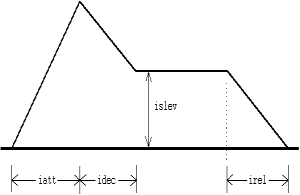
\includegraphics[scale=1]{adsr} 


 Picture of an ADSR envelope.


  The length of the sustain is calculated from the length of the note. This means \emph{adsr}
 is not suitable for use with MIDI events. The opcode \emph{madsr}
 uses the \emph{linsegr}
 mechanism, and so can be used in MIDI applications. The opcode \emph{mxadsr}
 is identical to \emph{madsr}
 except it uses exponential, rather than linear, line segments. 


 \emph{mxadsr}
 is new in Csound version 3.51. 
\subsection*{See Also}


 \emph{adsr}
, \emph{madsr}
, \emph{xadsr}

\subsection*{Credits}


 November 2002. Thanks to Rasmus Ekman, added documentation for the \emph{ireltim}
 parameter.


 November 2003. Thanks to Kanata Motohashi, fixed the link to the \emph{linsegr}
 opcode.
%\hline 


\begin{comment}
\begin{tabular}{lcr}
Previous &Home &Next \\
mute &Up &nchnls

\end{tabular}


\end{document}
\end{comment}

\newpage
%\begin{comment}
\documentclass[10pt]{article}
\usepackage{fullpage, graphicx, url}
\setlength{\parskip}{1ex}
\setlength{\parindent}{0ex}
\title{n Statement}
\begin{document}


\begin{tabular}{ccc}
The Alternative Csound Reference Manual & & \\
Previous & &Next

\end{tabular}

%\hline 
\end{comment}
\section{n Statement}
n�--� Repeats a section. \subsection*{Description}


  Repeats a section from the referenced \emph{m statement}
. 
\subsection*{Syntax}


 \textbf{n}
 p1
\subsection*{Initialization}


 \emph{p1}
 -- Name of mark to repeat. 
\subsection*{Performance}


  This can be helpful in setting a up verse and chorus structure in the score. Names may contain letters and numerals. 
\subsection*{Credits}


 


 


\begin{tabular}{cccc}
Author: John ffitch &University of Bath/Codemist Ltd. &Bath, UK &April 1998

\end{tabular}



 


 New in Csound version 3.48
%\hline 


\begin{comment}
\begin{tabular}{lcr}
Previous &Home &Next \\
m Statement (Mark Statement) &Up &q Statement

\end{tabular}


\end{document}
\end{comment}

\begin{comment}
\documentclass[10pt]{article}
\usepackage{fullpage, graphicx, url}
\setlength{\parskip}{1ex}
\setlength{\parindent}{0ex}
\title{nchnls}
\begin{document}


\begin{tabular}{ccc}
The Alternative Csound Reference Manual & & \\
Previous & &Next

\end{tabular}

%\hline 
\end{comment}
\section{nchnls}
nchnls�--� Sets the number of channels of audio output. \subsection*{Description}


  These statements are global value \emph{assignments}
, made at the beginning of an orchestra, before any instrument block is defined. Their function is to set certain \emph{reserved symbol variables}
 that are required for performance. Once set, these reserved symbols can be used in expressions anywhere in the orchestra. 
\subsection*{Syntax}


 \textbf{nchnls}
 = iarg
\subsection*{Initialization}


 \emph{nchnls}
 = (optional) -- set number of channels of audio output to \emph{iarg}
. (1 = mono, 2 = stereo, 4 = quadraphonic.) The default value is 1 (mono). 


  In addition, any \emph{global variable}
 can be initialized by an \emph{init-time assignment}
 anywhere before the first \emph{instr statement}
. All of the above assignments are run as instrument 0 (i-pass only) at the start of real performance. 
\subsection*{See Also}


 \emph{kr}
, \emph{ksmps}
, \emph{sr}

%\hline 


\begin{comment}
\begin{tabular}{lcr}
Previous &Home &Next \\
mxadsr &Up &nestedap

\end{tabular}


\end{document}
\end{comment}

\newpage
\begin{comment}
\documentclass[10pt]{article}
\usepackage{fullpage, graphicx, url}
\setlength{\parskip}{1ex}
\setlength{\parindent}{0ex}
\title{nestedap}
\begin{document}


\begin{tabular}{ccc}
The Alternative Csound Reference Manual & & \\
Previous & &Next

\end{tabular}

%\hline 
\end{comment}
\section{nestedap}
nestedap�--� Three different nested all-pass filters. \subsection*{Description}


  Three different nested all-pass filters, useful for implementing reverbs. 
\subsection*{Syntax}


 ar \textbf{nestedap}
 asig, imode, imaxdel, idel1, igain1 [, idel2] [, igain2] [, idel3] [, igain3] [, istor]
\subsection*{Initialization}


 \emph{imode}
 -- operating mode of the filter: 


 
\begin{itemize}
\item 

 1 = simple all-pass filter

\item 

 2 = single nested all-pass filter

\item 

 3 = double nested all-pass filter


\end{itemize}


 \emph{idel1}
, \emph{idel2}
, \emph{idel3}
 -- delay times of the filter stages. Delay times are in seconds and must be greater than zero. \emph{idel1}
 must be greater than the sum of \emph{idel2}
 and \emph{idel3}
. 


 \emph{igain1}
, \emph{igain2}
, \emph{igain3}
 -- gain of the filter stages. 


 \emph{imaxdel}
 -- will be necessary if k-rate delays are implemented. Not currently used. 


 \emph{istor}
 -- Skip initialization if non-zero (default: 0). 
\subsection*{Performance}


 \emph{asig}
 -- input signal 


  If \emph{imode}
 = 1, the filter takes the form: 


 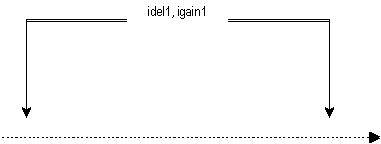
\includegraphics[scale=1]{imode1} 


 Picture of imode 1 filter.


  If \emph{imode}
 = 2, the filter takes the form: 


 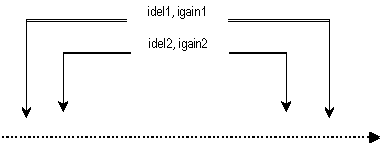
\includegraphics[scale=1]{imode2} 


 Picture of imode 2 filter.


  If \emph{imode}
 = 3, the filter takes the form: 


 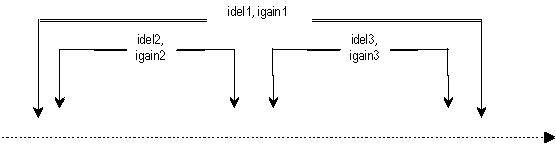
\includegraphics[scale=1]{imode3} 


 Picture of imode 3 filter.
\subsection*{Examples}


  Here is an example of the nestedap opcode. It uses the files \emph{nestedap.orc}
, \emph{nestedap.sco}
, and \emph{beats.wav}
. 


 \textbf{Example 1. Example of the nestedap opcode.}

\begin{lstlisting}
/* nestedap.orc */
sr = 44100
kr = 4410
ksmps = 10
nchnls = 2

instr 5
  insnd     =           p4
  gasig     diskin insnd, 1
endin

instr 10
  imax      =           1
  idel1     =           p4/1000
  igain1    =           p5
  idel2     =           p6/1000
  igain2    =           p7
  idel3     =           p8/1000
  igain3    =           p9
  idel4     =           p10/1000
  igain4    =           p11
  idel5     =           p12/1000
  igain5    =           p13
  idel6     =           p14/1000
  igain6    =           p15

  afdbk     init 0

  aout1     nestedap gasig+afdbk*.4, 3, imax, idel1, igain1, idel2, igain2, idel3, igain3
  
  aout2     nestedap aout1, 2, imax, idel4, igain4, idel5, igain5

  aout      nestedap aout2, 1, imax, idel6, igain6

  afdbk     butterlp aout, 1000

            outs gasig+(aout+aout1)/2, gasig-(aout+aout1)/2
  
gasig     =           0
endin
/* nestedap.orc */
        
\end{lstlisting}
\begin{lstlisting}
/* nestedap.sco */
f1 0 8192 10 1

; Diskin
;   Sta  Dur  Soundin
i5  0    3    "beats.wav"

; Reverb
;   St  Dur  Del1 Gn1  Del2  Gn2  Del3  Gn3  Del4  Gn4  Del5  Gn5  Del6  Gn6
i10 0   4    97   .11  23   .07   43   .09   72    .2   53    .2   119   .3
e
/* nestedap.sco */
        
\end{lstlisting}
\subsection*{Credits}


 


 


\begin{tabular}{cc}
Author: Hans Mikelson &February 1999

\end{tabular}



 


 New in Csound version 3.53


 The example was updated May 2002, thanks to Hans Mikelson
%\hline 


\begin{comment}
\begin{tabular}{lcr}
Previous &Home &Next \\
nchnls &Up &nlfilt

\end{tabular}


\end{document}
\end{comment}

\newpage
\begin{comment}
\documentclass[10pt]{article}
\usepackage{fullpage, graphicx, url}
\setlength{\parskip}{1ex}
\setlength{\parindent}{0ex}
\title{nlfilt}
\begin{document}


\begin{tabular}{ccc}
The Alternative Csound Reference Manual & & \\
Previous & &Next

\end{tabular}

%\hline 
\end{comment}
\section{nlfilt}
nlfilt�--� A filter with a non-linear effect. \subsection*{Description}


  Implements the filter: 


 Y\{n\}�=a�Y\{n-1\}�+�b�Y\{n-2\}�+�d�Y\^{}2\{n-L\}�+�X\{n\}�-�C�\\ 
 ������
 described in Dobson and Fitch (ICMC'96) \subsection*{Syntax}


 ar \textbf{nlfilt}
 ain, ka, kb, kd, kC, kL
\subsection*{Performance}


 


 
\begin{enumerate}
\item 

  Non-linear effect. The range of parameters are: 


 ��a�=�b�=�0\\ 
 ��d�=�0.8,�0.9,�0.7\\ 
 ��C�=�0.4,�0.5,�0.6\\ 
 ��L�=�20\\ 
 ������������
 This affects the lower register most but there are audible effects over the whole range. We suggest that it may be useful for coloring drums, and for adding arbitrary highlights to notes. 
\item 

  Low Pass with non-linear. The range of parameters are: 


 ��a�=�0.4\\ 
 ��b�=�0.2\\ 
 ��d�=�0.7\\ 
 ��C�=�0.11\\ 
 ��L�=�20,�...�200\\ 
 ������������
 There are instability problems with this variant but the effect is more pronounced of the lower register, but is otherwise much like the pure comb. Short values of \emph{L}
 can add attack to a sound. 
\item 

  High Pass with non-linear. The range of parameters are: 


 ��a�=�0.35\\ 
 ��b�=�-0.3\\ 
 ��d�=�0.95\\ 
 ��C�=�0,2,�...�0.4\\ 
 ��L�=�200\\ 
 ������������

\item 

  High Pass with non-linear. The range of parameters are: 


 ��a�=�0.7\\ 
 ��b�=�-0.2,�...�0.5\\ 
 ��d�=�0.9\\ 
 ��C�=�0.12,�...�0.24\\ 
 ��L�=�500,�10\\ 
 ������������
 The high pass version is less likely to oscillate. It adds scintillation to medium-high registers. With a large delay \emph{L}
 it is a little like a reverberation, while with small values there appear to be formant-like regions. There are arbitrary color changes and resonances as the pitch changes. Works well with individual notes. 

\end{enumerate}


 


\begin{tabular}{cc}
Warning &\textbf{Warning}
 \\
� &

  The ``useful'' ranges of parameters are not yet mapped. 


\end{tabular}

\subsection*{Credits}


 


 


\begin{tabular}{cccc}
Author: John ffitch &University of Bath/Codemist Ltd. &Bath, UK &1997

\end{tabular}



 
%\hline 


\begin{comment}
\begin{tabular}{lcr}
Previous &Home &Next \\
nestedap &Up &noise

\end{tabular}


\end{document}
\end{comment}

\newpage
\begin{comment}
\documentclass[10pt]{article}
\usepackage{fullpage, graphicx, url}
\setlength{\parskip}{1ex}
\setlength{\parindent}{0ex}
\title{noise}
\begin{document}


\begin{tabular}{ccc}
The Alternative Csound Reference Manual & & \\
Previous & &Next

\end{tabular}

%\hline 
\end{comment}
\section{noise}
noise�--� A white noise generator with an IIR lowpass filter. \subsection*{Description}


  A white noise generator with an IIR lowpass filter. 
\subsection*{Syntax}


 ar \textbf{noise}
 xamp, kbeta
\subsection*{Initialization}


 \emph{ioffset}
 -- the delay before the first impulse. If it is negative, the value is taken as the number of samples, otherwise it is in seconds. Default is zero. 
\subsection*{Performance}


 \emph{xamp}
 -- amplitude of final output 


 \emph{kbeta}
 -- beta of the lowpass filter. Should be in the range of 0 to 1. 


  The filter equation is: 


 y\_n�=�sqrt(1-beta\^{}2)�*�x\_n�+�beta�Y\_(n-1)\\ 
 ������
 where \emph{x\_n}
 is white noise. \subsection*{Examples}


  Here is an example of the noise opcode. It uses the files \emph{noise.orc}
 and \emph{noise.sco}
. 


 \textbf{Example 1. Example of the noise opcode.}

\begin{lstlisting}
/* noise.orc */
; Initialize the global variables.
sr = 44100
kr = 4410
ksmps = 10
nchnls = 1

; Instrument #1.
instr 1
  kamp = 30000

  ; Change the beta value linearly from 0 to 1.
  kbeta line 0, p3, 1

  a1 noise kamp, kbeta
  out a1
endin
/* noise.orc */
        
\end{lstlisting}
\begin{lstlisting}
/* noise.sco */
; Play Instrument #1 for one second.
i 1 0 1
e
/* noise.sco */
        
\end{lstlisting}
\subsection*{Credits}


 


 


\begin{tabular}{cccc}
Author: John ffitch &University of Bath, Codemist. Ltd. &Bath, UK &December 2000

\end{tabular}



 


 Example written by Kevin Conder.


 New in Csound version 4.10
%\hline 


\begin{comment}
\begin{tabular}{lcr}
Previous &Home &Next \\
nlfilt &Up &noteoff

\end{tabular}


\end{document}
\end{comment}

\newpage
\begin{comment}
\documentclass[10pt]{article}
\usepackage{fullpage, graphicx, url}
\setlength{\parskip}{1ex}
\setlength{\parindent}{0ex}
\title{noteoff}
\begin{document}


\begin{tabular}{ccc}
The Alternative Csound Reference Manual & & \\
Previous & &Next

\end{tabular}

%\hline 
\end{comment}
\section{noteoff}
noteoff�--� Send a noteoff message to the MIDI OUT port. \subsection*{Description}


  Send a noteoff message to the MIDI OUT port. 
\subsection*{Syntax}


 \textbf{noteoff}
 ichn, inum, ivel
\subsection*{Initialization}


 \emph{ichn}
 -- MIDI channel number (1-16) 


 \emph{inum}
 -- note number (0-127) 


 \emph{ivel}
 -- velocity (0-127) 
\subsection*{Performance}


 \emph{noteon}
 (i-rate note on) and \emph{noteoff}
 (i-rate note off) are the simplest MIDI OUT opcodes. \emph{noteon}
 sends a MIDI noteon message to MIDI OUT port, and \emph{noteoff}
 sends a noteoff message. A \emph{noteon}
 opcode must always be followed by an \emph{noteoff}
 with the same channel and number inside the same instrument, otherwise the note will play endlessly. 


  These \emph{noteon}
 and \emph{noteoff}
 opcodes are useful only when introducing a \emph{timout}
 statement to play a non-zero duration MIDI note. For most purposes, it is better to use \emph{noteondur}
 and \emph{noteondur2}
. 
\subsection*{See Also}


 \emph{noteon}
, \emph{noteondur}
, \emph{noteondur2}

\subsection*{Credits}


 


 


\begin{tabular}{cc}
Author: Gabriel Maldonado &Italy

\end{tabular}



 


 New in Csound version 3.47


 Thanks goes to Rasmus Ekman for pointing out the correct MIDI channel and controller number ranges.
%\hline 


\begin{comment}
\begin{tabular}{lcr}
Previous &Home &Next \\
noise &Up &noteon

\end{tabular}


\end{document}
\end{comment}

\newpage
\begin{comment}
\documentclass[10pt]{article}
\usepackage{fullpage, graphicx, url}
\setlength{\parskip}{1ex}
\setlength{\parindent}{0ex}
\title{noteon}
\begin{document}


\begin{tabular}{ccc}
The Alternative Csound Reference Manual & & \\
Previous & &Next

\end{tabular}

%\hline 
\end{comment}
\section{noteon}
noteon�--� Send a noteon message to the MIDI OUT port. \subsection*{Description}


  Send a noteon message to the MIDI OUT port. 
\subsection*{Syntax}


 \textbf{noteon}
 ichn, inum, ivel
\subsection*{Initialization}


 \emph{ichn}
 -- MIDI channel number (1-16) 


 \emph{inum}
 -- note number (0-127) 


 \emph{ivel}
 -- velocity (0-127) 
\subsection*{Performance}


 \emph{noteon}
 (i-rate note on) and \emph{noteoff}
 (i-rate note off) are the simplest MIDI OUT opcodes. \emph{noteon}
 sends a MIDI noteon message to MIDI OUT port, and \emph{noteoff}
 sends a noteoff message. A \emph{noteon}
 opcode must always be followed by an \emph{noteoff}
 with the same channel and number inside the same instrument, otherwise the note will play endlessly. 


  These \emph{noteon}
 and \emph{noteoff}
 opcodes are useful only when introducing a \emph{timout}
 statement to play a non-zero duration MIDI note. For most purposes, it is better to use \emph{noteondur}
 and \emph{noteondur2}
. 
\subsection*{See Also}


 \emph{noteoff}
, \emph{noteondur}
, \emph{noteondur2}

\subsection*{Credits}


 


 


\begin{tabular}{cc}
Author: Gabriel Maldonado &Italy

\end{tabular}



 


 New in Csound version 3.47


 Thanks goes to Rasmus Ekman for pointing out the correct MIDI channel and controller number ranges.
%\hline 


\begin{comment}
\begin{tabular}{lcr}
Previous &Home &Next \\
noteoff &Up &noteondur

\end{tabular}


\end{document}
\end{comment}

\newpage
\begin{comment}
\documentclass[10pt]{article}
\usepackage{fullpage, graphicx, url}
\setlength{\parskip}{1ex}
\setlength{\parindent}{0ex}
\title{noteondur}
\begin{document}


\begin{tabular}{ccc}
The Alternative Csound Reference Manual & & \\
Previous & &Next

\end{tabular}

%\hline 
\end{comment}
\section{noteondur}
noteondur�--� Sends a noteon and a noteoff MIDI message both with the same channel, number and velocity. \subsection*{Description}


  Sends a noteon and a noteoff MIDI message both with the same channel, number and velocity. 
\subsection*{Syntax}


 \textbf{noteondur}
 ichn, inum, ivel, idur
\subsection*{Initialization}


 \emph{ichn}
 -- MIDI channel number (1-16) 


 \emph{inum}
 -- note number (0-127) 


 \emph{ivel}
 -- velocity (0-127) 


 \emph{idur}
 -- how long, in seconds, this note should last. 
\subsection*{Performance}


 \emph{noteondur}
 (i-rate note on with duration) sends a noteon and a noteoff MIDI message both with the same channel, number and velocity. Noteoff message is sent after \emph{idur}
 seconds are elapsed by the time \emph{noteondur}
 was active. 


 \emph{noteondur}
 differs from \emph{noteondur2}
 in that \emph{noteondur}
 truncates note duration when current instrument is deactivated by score or by real-time playing, while \emph{noteondur2}
 will extend performance time of current instrument until \emph{idur}
 seconds have elapsed. In real-time playing, it is suggested to use \emph{noteondur}
 also for undefined durations, giving a large \emph{idur}
 value. 


  Any number of \emph{noteondur}
 opcodes can appear in the same Csound instrument, allowing chords to be played by a single instrument. 
\subsection*{See Also}


 \emph{noteoff}
, \emph{noteon}
, \emph{noteondur2}

\subsection*{Credits}


 


 


\begin{tabular}{cc}
Author: Gabriel Maldonado &Italy

\end{tabular}



 


 New in Csound version 3.47


 Thanks goes to Rasmus Ekman for pointing out the correct MIDI channel and controller number ranges.
%\hline 


\begin{comment}
\begin{tabular}{lcr}
Previous &Home &Next \\
noteon &Up &noteondur2

\end{tabular}


\end{document}
\end{comment}

\newpage
\begin{comment}
\documentclass[10pt]{article}
\usepackage{fullpage, graphicx, url}
\setlength{\parskip}{1ex}
\setlength{\parindent}{0ex}
\title{noteondur2}
\begin{document}


\begin{tabular}{ccc}
The Alternative Csound Reference Manual & & \\
Previous & &Next

\end{tabular}

%\hline 
\end{comment}
\section{noteondur2}
noteondur2�--� Sends a noteon and a noteoff MIDI message both with the same channel, number and velocity. \subsection*{Description}


  Sends a noteon and a noteoff MIDI message both with the same channel, number and velocity. 
\subsection*{Syntax}


 \textbf{noteondur2}
 ichn, inum, ivel, idur
\subsection*{Initialization}


 \emph{ichn}
 -- MIDI channel number (1-16) 


 \emph{inum}
 -- note number (0-127) 


 \emph{ivel}
 -- velocity (0-127) 


 \emph{idur}
 -- how long, in seconds, this note should last. 
\subsection*{Performance}


 \emph{noteondur2}
 (i-rate note on with duration) sends a noteon and a noteoff MIDI message both with the same channel, number and velocity. Noteoff message is sent after \emph{idur}
 seconds are elapsed by the time \emph{noteondur2}
 was active. 


 \emph{noteondur}
 differs from \emph{noteondur2}
 in that \emph{noteondur}
 truncates note duration when current instrument is deactivated by score or by real-time playing, while \emph{noteondur2}
 will extend performance time of current instrument until \emph{idur}
 seconds have elapsed. In real-time playing, it is suggested to use \emph{noteondur}
 also for undefined durations, giving a large \emph{idur}
 value. 


  Any number of \emph{noteondur2}
 opcodes can appear in the same Csound instrument, allowing chords to be played by a single instrument. 
\subsection*{See Also}


 \emph{noteoff}
, \emph{noteon}
, \emph{noteondur}

\subsection*{Credits}


 


 


\begin{tabular}{cc}
Author: Gabriel Maldonado &Italy

\end{tabular}



 


 New in Csound version 3.47


 Thanks goes to Rasmus Ekman for pointing out the correct MIDI channel and controller number ranges.
%\hline 


\begin{comment}
\begin{tabular}{lcr}
Previous &Home &Next \\
noteondur &Up &notnum

\end{tabular}


\end{document}
\end{comment}

\newpage
\begin{comment}
\documentclass[10pt]{article}
\usepackage{fullpage, graphicx, url}
\setlength{\parskip}{1ex}
\setlength{\parindent}{0ex}
\title{!=}
\begin{document}


\begin{tabular}{ccc}
The Alternative Csound Reference Manual & & \\
Previous & &Next

\end{tabular}

%\hline 
\end{comment}
\section{!=}
!=�--� Determines if one value is not equal to another. \subsection*{Description}


  Determines if one value is not equal to another. 
\subsection*{Syntax}


 (a \textbf{!=}
 b \textbf{?}
 v1 \textbf{:}
 v2)


  where \emph{a}
, \emph{b}
, \emph{v1}
 and \emph{v2}
 may be expressions, but \emph{a}
, \emph{b}
 not audio-rate. 
\subsection*{Performance}


  In the above conditionals, \emph{a}
 and \emph{b}
 are first compared. If the indicated relation is true (\emph{a}
 greater than \emph{b}
, \emph{a}
 less than \emph{b}
, \emph{a}
 greater than or equal to \emph{b}
, \emph{a}
 less than or equal to \emph{b}
, \emph{a}
 equal to \emph{b}
, \emph{a}
 not equal to \emph{b}
), then the conditional expression has the value of \emph{v1}
; if the relation is false, the expression has the value of \emph{v2}
. (For convenience, a sole ``\emph{=}
`` will function as ``\emph{= =}
``.) 


  NB.: If \emph{v1}
 or \emph{v2}
 are expressions, these will be evaluated before the conditional is determined. 


  In terms of binding strength, all conditional operators (i.e. the relational operators (\emph{$<$}
, etc.), and \emph{?}
, and \emph{:}
 ) are weaker than the arithmetic and logical operators (\emph{+}
, \emph{-}
, \emph{*}
, \emph{/}
, \emph{\&}
 and \emph{||}
). 


  These are \emph{operators}
 not \emph{opcodes}
. Therefore, they can be used within orchestra statements, but do not form complete statements themselves. 
\subsection*{Examples}


  Here is an example of the != opcode. It uses the files \emph{notequal.orc}
 and \emph{notequal.sco}
. 


 \textbf{Example 1. Example of the != opcode.}

\begin{lstlisting}
/* notequal.orc */
; Initialize the global variables.
sr = 44100
kr = 44100
ksmps = 1
nchnls = 1

; Instrument #1.
instr 1
  ; Get the 4th p-field from the score.
  k1 =  p4

  ; Is it not equal to 3? (1 = true, 0 = false)
  k2 = (p4 != 3 ? 1 : 0)

  ; Print the values of k1 and k2.
  printks "k1 = %f, k2 = %f\\n", 1, k1, k2
endin
/* notequal.orc */
        
\end{lstlisting}
\begin{lstlisting}
/* notequal.sco */
; Call Instrument #1 with a p4 = 2.
i 1 0 0.5 2
; Call Instrument #1 with a p4 = 3.
i 1 1 0.5 3
; Call Instrument #1 with a p4 = 4.
i 1 2 0.5 4
e
/* notequal.sco */
        
\end{lstlisting}
 Its output should include lines like this: \begin{lstlisting}
k1 = 2.000000, k2 = 1.000000
k1 = 3.000000, k2 = 0.000000
k1 = 4.000000, k2 = 1.000000
      
\end{lstlisting}
\subsection*{See Also}


 \emph{==}
, \emph{$>$=}
, \emph{$>$}
, \emph{$<$=}
, \emph{$<$}

\subsection*{Credits}


 Example written by Kevin Conder.
%\hline 


\begin{comment}
\begin{tabular}{lcr}
Previous &Home &Next \\
Orchestra Opcodes and Operators &Up &\#define

\end{tabular}


\end{document}
\end{comment}

\newpage
\begin{comment}
\documentclass[10pt]{article}
\usepackage{fullpage, graphicx, url}
\setlength{\parskip}{1ex}
\setlength{\parindent}{0ex}
\title{notnum}
\begin{document}


\begin{tabular}{ccc}
The Alternative Csound Reference Manual & & \\
Previous & &Next

\end{tabular}

%\hline 
\end{comment}
\section{notnum}
notnum�--� Get a note number from a MIDI event. \subsection*{Description}


  Get a note number from a MIDI event. 
\subsection*{Syntax}


 ival \textbf{notnum}

\subsection*{Performance}


  Get the MIDI byte value (0 - 127) denoting the note number of the current event. 
\subsection*{Examples}


  Here is an example of the notnum opcode. It uses the files \emph{notnum.orc}
 and \emph{notnum.sco}
. 


 \textbf{Example 1. Example of the notnum opcode.}

\begin{lstlisting}
/* notnum.orc */
; Initialize the global variables.
sr = 44100
kr = 4410
ksmps = 10
nchnls = 1

; Instrument #1.
instr 1
  i1 notnum

  print i1
endin
/* notnum.orc */
        
\end{lstlisting}
\begin{lstlisting}
/* notnum.sco */
; Play Instrument #1 for 12 seconds.
i 1 0 12
e
/* notnum.sco */
        
\end{lstlisting}
\subsection*{See Also}


 \emph{aftouch}
, \emph{ampmidi}
, \emph{cpsmidi}
, \emph{cpsmidib}
, \emph{midictrl}
, \emph{octmidi}
, \emph{octmidib}
, \emph{pchbend}
, \emph{pchmidi}
, \emph{pchmidib}
, \emph{veloc}

\subsection*{Credits}


 


 


\begin{tabular}{ccc}
Author: Barry L. Vercoe - Mike Berry &MIT - Mills &May 1997

\end{tabular}



 


 Example written by Kevin Conder.
%\hline 


\begin{comment}
\begin{tabular}{lcr}
Previous &Home &Next \\
noteondur2 &Up &nreverb

\end{tabular}


\end{document}
\end{comment}

\newpage
\begin{comment}
\documentclass[10pt]{article}
\usepackage{fullpage, graphicx, url}
\setlength{\parskip}{1ex}
\setlength{\parindent}{0ex}
\title{nreverb}
\begin{document}


\begin{tabular}{ccc}
The Alternative Csound Reference Manual & & \\
Previous & &Next

\end{tabular}

%\hline 
\end{comment}
\section{nreverb}
nreverb�--� A reverberator consisting of 6 parallel comb-lowpass filters. \subsection*{Description}


  This is a reverberator consisting of 6 parallel comb-lowpass filters being fed into a series of 5 allpass filters. \emph{nreverb}
 replaces \emph{reverb2}
 (version 3.48) and so both opcodes are identical. 
\subsection*{Syntax}


 ar \textbf{nreverb}
 asig, ktime, khdif [, iskip] [,inumCombs] [, ifnCombs] [, inumAlpas] [, ifnAlpas]
\subsection*{Initialization}


 \emph{iskip}
 (optional, default=0) -- Skip initialization if present and non-zero. 


 \emph{inumCombs}
 (optional) -- number of filter constants in comb filter. If omitted, the values default to the nreverb constants. New in Csound version 4.09. 


 \emph{ifnCombs}
 - function table with \emph{inumCombs}
 comb filter time values, followed the same number of gain values. The ftable should not be rescaled (use negative fgen number). Positive time values are in seconds. The time values are converted internally into number of samples, then set to the next greater prime number. If the time is negative, it is interpreted directly as time in sample frames, and no processing is done (except negation). New in Csound version 4.09. 


 \emph{inumAlpas}
, \emph{ifnAlpas}
 (optional) -- same as \emph{inumCombs/ifnCombs}
, for allpass filter. New in Csound 4.09. 
\subsection*{Performance}


  The input signal asig is reverberated for \emph{ktime}
 seconds. The parameter \emph{khdif}
 controls the high frequency diffusion amount. The values of \emph{khdif}
 should be from 0 to 1. If \emph{khdif}
 is set to 0 the all the frequencies decay with the same speed. If \emph{khdif}
 is 1, high frequencies decay faster than lower ones. If \emph{ktime}
 is inadvertently set to a non-positive number, \emph{ktime}
 will be reset automatically to 0.01. (New in Csound version 4.07.) 


  As of Csound version 4.09, \emph{nreverb}
 may read any number of comb and allpass filter from an ftable. 
\subsection*{Examples}


  Here is a simple example of the nreverb opcode. It uses the files \emph{nreverb.orc}
 and \emph{nreverb.sco}
. 


 \textbf{Example 1. Simple example of the nreverb opcode.}

\begin{lstlisting}
/* nreverb.orc */
; Initialize the global variables.
sr = 44100
kr = 4410
ksmps = 10
nchnls = 1

instr 1
  a1 oscil 10000, 440, 1
  a2 nreverb a1, 2.5, .3
  out a1 + a2 * .2
endin
/* nreverb.orc */
        
\end{lstlisting}
\begin{lstlisting}
/* nreverb.sco */
; Table 1: an ordinary sine wave.
f 1 0 32768 10 1 
         
i 1 0.0 0.5
i 1 1.0 0.5
i 1 2.0 0.5
i 1 3.0 0.5
i 1 4.0 0.5
e
/* nreverb.sco */
        
\end{lstlisting}


  Here is an example of the nreverb opcode using an ftable for filter constants. It uses the files \emph{nreverb\_ftable.orc}
, \emph{nreverb\_ftable.sco}
, and \emph{beats.wav}
. 


 \textbf{Example 2. An example of the nreverb opcode using an ftable for filter constants.}

\begin{lstlisting}
/* nreverb_ftable.orc */
; Initialize the global variables.
sr = 44100
kr = 4410
ksmps = 10
nchnls = 1

instr 1
  a1  soundin "beats.wav"
  a2  nreverb a1, 1.5, .75, 0, 8, 71, 4, 72
  out a1 + a2 * .4
endin
/* nreverb_ftable.orc */
        
\end{lstlisting}
\begin{lstlisting}
/* nreverb_ftable.sco */
; freeverb time constants, as direct (negative) sample, with arbitrary gains
f71 0 16   -2  -1116 -1188 -1277 -1356 -1422 -1491 -1557 -1617  0.8  0.79  0.78  0.77  0.76  0.75  0.74  0.73

f72 0 16   -2  -556 -441 -341 -225  0.7  0.72  0.74  0.76

i1 0 3
e
/* nreverb_ftable.sco */
        
\end{lstlisting}
\subsection*{Credits}


 


 


\begin{tabular}{ccc}
Authors: Paris Smaragdis (\emph{reverb2}
) &MIT, Cambridge &1995

\end{tabular}



 


 


 


\begin{tabular}{ccc}
Author: Richard Karpen (\emph{nreverb}
) &Seattle, Wash &1998

\end{tabular}



 
%\hline 


\begin{comment}
\begin{tabular}{lcr}
Previous &Home &Next \\
notnum &Up &nrpn

\end{tabular}


\end{document}
\end{comment}

\newpage
\begin{comment}
\documentclass[10pt]{article}
\usepackage{fullpage, graphicx, url}
\setlength{\parskip}{1ex}
\setlength{\parindent}{0ex}
\title{nrpn}
\begin{document}


\begin{tabular}{ccc}
The Alternative Csound Reference Manual & & \\
Previous & &Next

\end{tabular}

%\hline 
\end{comment}
\section{nrpn}
nrpn�--� Sends a Non-Registered Parameter Number to the MIDI OUT port. \subsection*{Description}


  Sends a NPRN (Non-Registered Parameter Number) message to the MIDI OUT port each time one of the input arguments changes. 
\subsection*{Syntax}


 \textbf{nrpn}
 kchan, kparmnum, kparmvalue
\subsection*{Performance}


 \emph{kchan}
 -- MIDI channel (1-16) 


 \emph{kparmnum}
 -- number of NRPN parameter 


 \emph{kparmvalue}
 -- value of NRPN parameter 


  This opcode sends new message when the MIDI translated value of one of the input arguments changes. It operates at k-rate. Useful with the MIDI instruments that recognize NRPNs (for example with the newest sound-cards with internal MIDI synthesizer such as SB AWE32, AWE64, GUS etc. in which each patch parameter can be changed during the performance via NRPN) 
\subsection*{Credits}


 


 


\begin{tabular}{ccc}
Author: Gabriel Maldonado &Italy &1998

\end{tabular}



 


 New in Csound version 3.492


 Thanks goes to Rasmus Ekman for pointing out the correct MIDI channel and controller number ranges.
%\hline 


\begin{comment}
\begin{tabular}{lcr}
Previous &Home &Next \\
nreverb &Up &nsamp

\end{tabular}


\end{document}
\end{comment}

\newpage
\begin{comment}
\documentclass[10pt]{article}
\usepackage{fullpage, graphicx, url}
\setlength{\parskip}{1ex}
\setlength{\parindent}{0ex}
\title{nsamp}
\begin{document}


\begin{tabular}{ccc}
The Alternative Csound Reference Manual & & \\
Previous & &Next

\end{tabular}

%\hline 
\end{comment}
\section{nsamp}
nsamp�--� Returns the number of samples loaded into a stored function table number. \subsection*{Description}


  Returns the number of samples loaded into a stored function table number. 
\subsection*{Syntax}


 \textbf{nsamp}
(x) (init-rate args only)
\subsection*{Performance}


  Returns the number of samples loaded into stored function table number \emph{x}
 by \emph{GEN01}
. This is useful when a sample is shorter than the power-of-two function table that holds it. New in Csound version 3.49. 
\subsection*{Examples}


  Here is an example of the nsamp opcode. It uses the files \emph{nsamp.orc}
, \emph{nsamp.sco}
, and \emph{mary.wav}
. 


 \textbf{Example 1. Example of the nsamp opcode.}

\begin{lstlisting}
/* nsamp.orc */
; Initialize the global variables.
sr = 44100
kr = 4410
ksmps = 10
nchnls = 1

; Instrument #1.
instr 1
  ; Print out the size (in samples) of Table #1.
  isz = nsamp(1)
  print isz
endin
/* nsamp.orc */
        
\end{lstlisting}
\begin{lstlisting}
/* nsamp.sco */
; Table #1: Use an audio file.
f 1 0 262144 1 "mary.wav" 0 0 0

; Play Instrument #1 for 1 second.
i 1 0 1
e
/* nsamp.sco */
        
\end{lstlisting}
 Since the audio file ``mary.wav'' has 154390 samples, its output should include a line like this: \begin{lstlisting}
instr 1:  isz = 154390.000
      
\end{lstlisting}
\subsection*{See Also}


 \emph{ftchnls}
, \emph{ftlen}
, \emph{ftlptim}
, \emph{ftsr}

\subsection*{Credits}


 


 


\begin{tabular}{ccc}
Author: Gabriel Maldonado &Italy &October 1998

\end{tabular}



 


 Example written by Kevin Conder.
%\hline 


\begin{comment}
\begin{tabular}{lcr}
Previous &Home &Next \\
nrpn &Up &nstrnum

\end{tabular}


\end{document}
\end{comment}

\newpage
\begin{comment}
\documentclass[10pt]{article}
\usepackage{fullpage, graphicx, url}
\setlength{\parskip}{1ex}
\setlength{\parindent}{0ex}
\title{nstrnum}
\begin{document}


\begin{tabular}{ccc}
The Alternative Csound Reference Manual & & \\
Previous & &Next

\end{tabular}

%\hline 
\end{comment}
\section{nstrnum}
nstrnum�--� Returns the number of a named instrument. \subsection*{Description}


  Returns the number of a named instrument. 
\subsection*{Syntax}


 insno \textbf{nstrnum}
 ``name''
\subsection*{Initialization}


 \emph{insno}
 -- the instrument number of the named instrument. 
\subsection*{Performance}


 \emph{``name''}
 -- the named instrument's name. 


  If an instrument with the specified name does not exist, an init error occurs, and -1 is returned. 
\subsection*{Credits}


 


 


\begin{tabular}{ccc}
Author: Istvan Varga &New in version 4.23 &Written in the year 2002.

\end{tabular}



 
%\hline 


\begin{comment}
\begin{tabular}{lcr}
Previous &Home &Next \\
nsamp &Up &ntrpol

\end{tabular}


\end{document}
\end{comment}

\newpage
\begin{comment}
\documentclass[10pt]{article}
\usepackage{fullpage, graphicx, url}
\setlength{\parskip}{1ex}
\setlength{\parindent}{0ex}
\title{ntrpol}
\begin{document}


\begin{tabular}{ccc}
The Alternative Csound Reference Manual & & \\
Previous & &Next

\end{tabular}

%\hline 
\end{comment}
\section{ntrpol}
ntrpol�--� Calculates the weighted mean value of two input signals. \subsection*{Description}


  Calculates the weighted mean value (i.e. linear interpolation) of two input signals 
\subsection*{Syntax}


 ar \textbf{ntrpol}
 asig1, asig2, kpoint [, imin] [, imax]


 ir \textbf{ntrpol}
 isig1, isig2, ipoint [, imin] [, imax]


 kr \textbf{ntrpol}
 ksig1, ksig2, kpoint [, imin] [, imax]
\subsection*{Initialization}


 \emph{imin}
 -- minimum xpoint value (optional, default 0) 


 \emph{imax}
 -- maximum xpoint value (optional, default 1) 
\subsection*{Performance}


 \emph{xsig1}
, \emph{xsig2}
 -- input signals 


 \emph{xpoint}
 -- interpolation point between the two values 


 \emph{ntrpol}
 opcode outputs the linear interpolation between two input values. \emph{xpoint}
 is the distance of evaluation point from the first value. With the default values of \emph{imin}
 and \emph{imax}
, (0 and 1) a zero value indicates no distance from the first value and the maximum distance from the second one. With a 0.5 value, \emph{ntrpol}
 will output the mean value of the two inputs, indicating the exact half point between \emph{xsig1}
 and \emph{xsig2}
. A 1 value indicates the maximum distance from the first value and no distance from the second one. The range of \emph{xpoint}
 can be also defined with \emph{imin}
 and \emph{imax}
 to make its management easier. 


  These opcodes are useful for crossfading two signals. 
\subsection*{Credits}


 


 


\begin{tabular}{ccc}
Author: Gabriel Maldonado &Italy &October 1998

\end{tabular}



 


 New in Csound version 3.49
%\hline 


\begin{comment}
\begin{tabular}{lcr}
Previous &Home &Next \\
nstrnum &Up &octave

\end{tabular}


\end{document}
\end{comment}

\newpage
\begin{comment}
\documentclass[10pt]{article}
\usepackage{fullpage, graphicx, url}
\setlength{\parskip}{1ex}
\setlength{\parindent}{0ex}
\title{octave}
\begin{document}


\begin{tabular}{ccc}
The Alternative Csound Reference Manual & & \\
Previous & &Next

\end{tabular}

%\hline 
\end{comment}
\section{octave}
octave�--� Calculates a factor to raise/lower a frequency by a given amount of octaves. \subsection*{Description}


  Calculates a factor to raise/lower a frequency by a given amount of octaves. 
\subsection*{Syntax}


 \textbf{octave}
(x)


  This function works at a-rate, i-rate, and k-rate. 
\subsection*{Initialization}


 \emph{x}
 -- a value expressed in octaves. 
\subsection*{Performance}


  The value returned by the \emph{octave}
 function is a factor. You can multiply a frequency by this factor to raise/lower it by the given amount of octaves. 
\subsection*{Examples}


  Here is an example of the octave opcode. It uses the files \emph{octave.orc}
 and \emph{octave.sco}
. 


 \textbf{Example 1. Example of the octave opcode.}

\begin{lstlisting}
/* octave.orc */
; Initialize the global variables.
sr = 44100
kr = 4410
ksmps = 10
nchnls = 1

; Instrument #1.
instr 1
  ; The root note is A above middle-C (440 Hz)
  iroot = 440

  ; Raise the root note by two octaves.
  ioctaves = 2

  ; Calculate the new note.
  ifactor = octave(ioctaves)
  inew = iroot * ifactor

  ; Print out of all of the values.
  print iroot
  print ifactor
  print inew
endin
/* octave.orc */
        
\end{lstlisting}
\begin{lstlisting}
/* octave.sco */
; Play Instrument #1 for one second.
i 1 0 1
e
/* octave.sco */
        
\end{lstlisting}
 Its output should include lines like: \begin{lstlisting}
instr 1:  iroot = 440.000
instr 1:  ifactor = 4.000
instr 1:  inew = 1760.149
      
\end{lstlisting}
\subsection*{See Also}


 \emph{cent}
, \emph{db}
, \emph{semitone}

\subsection*{Credits}


 Example written by Kevin Conder.


 New in version 4.16
%\hline 


\begin{comment}
\begin{tabular}{lcr}
Previous &Home &Next \\
ntrpol &Up &octcps

\end{tabular}


\end{document}
\end{comment}

\newpage
\begin{comment}
\documentclass[10pt]{article}
\usepackage{fullpage, graphicx, url}
\setlength{\parskip}{1ex}
\setlength{\parindent}{0ex}
\title{octcps}
\begin{document}


\begin{tabular}{ccc}
The Alternative Csound Reference Manual & & \\
Previous & &Next

\end{tabular}

%\hline 
\end{comment}
\section{octcps}
octcps�--� Converts a cycles-per-second value to octave-point-decimal. \subsection*{Description}


  Converts a cycles-per-second value to octave-point-decimal. 
\subsection*{Syntax}


 \textbf{octcps}
 (cps) (init- or control-rate args only)


  where the argument within the parentheses may be a further expression. 
\subsection*{Performance}


  These are really \emph{value converters}
 with a special function of manipulating pitch data. 


  Data concerning pitch and frequency can exist in any of the following forms: 


 \textbf{Table 1. Pitch and Frequency Values}



\begin{tabular}{ccc}
NameAbbreviation & & \\
octave point pitch-class (8ve.pc)pch &octave point decimaloct &cycles per secondcps

\end{tabular}



  The first two forms consist of a whole number, representing octave registration, followed by a specially interpreted fractional part. For \emph{pch}
, the fraction is read as two decimal digits representing the 12 equal-tempered pitch classes from .00 for C to.11 for B. For \emph{oct}
, the fraction is interpreted as a true decimal fractional part of an octave. The two fractional forms are thus related by the factor 100/12. In both forms, the fraction is preceded by a whole number octave index such that 8.00 represents Middle C, 9.00 the C above, etc. Thus A440 can be represented alternatively by 440 (\emph{cps}
),8.09 (\emph{pch}
), or 8.75 (\emph{oct}
). Microtonal divisions of the \emph{pch}
 semitone can be encoded by using more than two decimal places. 


  The mnemonics of the pitch conversion units are derived from morphemes of the forms involved, the second morpheme describing the source and the first morpheme the object (result). Thus \emph{cpspch}
(8.09) will convert the pitch argument 8.09 to its \emph{cps}
 (or Hertz) equivalent, giving the value of 440. Since the argument is constant over the duration of the note, this conversion will take place at i-time, before any samples for the current note are produced. 


  By contrast, the conversion \emph{cpsoct}
(8.75 + k1) which gives the value of A440 transposed by the octave interval \emph{k1}
. The calculation will be repeated every k-period since that is the rate at which \emph{k1}
 varies. 


 


\begin{tabular}{cc}
\textbf{Note}
 \\
� &

  The conversion from \emph{pch}
 or \emph{oct}
 into \emph{cps}
 is not a linear operation but involves an exponential process that could be time-consuming when executed repeatedly. Csound now uses a built-in table lookup to do this efficiently, even at audio rates. 


\end{tabular}

\subsection*{Examples}


  Here is an example of the octcps opcode. It uses the files \emph{octcps.orc}
 and \emph{octcps.sco}
. 


 \textbf{Example 1. Example of the octcps opcode.}

\begin{lstlisting}
/* octcps.orc */
; Initialize the global variables.
sr = 44100
kr = 4410
ksmps = 10
nchnls = 1

; Instrument #1.
instr 1
  ; Convert a cycles-per-second value into an 
  ; octave value.
  icps = 440
  ioct = octcps(icps)

  print ioct
endin
/* octcps.orc */
        
\end{lstlisting}
\begin{lstlisting}
/* octcps.sco */
; Play Instrument #1 for one second.
i 1 0 1
e
/* octcps.sco */
        
\end{lstlisting}
 Its output should include a line like this: \begin{lstlisting}
instr 1:  ioct = 8.750
      
\end{lstlisting}
\subsection*{See Also}


 \emph{cpsoct}
, \emph{cpspch}
, \emph{octpch}
, \emph{pchoct}

\subsection*{Credits}


 Example written by Kevin Conder.
%\hline 


\begin{comment}
\begin{tabular}{lcr}
Previous &Home &Next \\
octave &Up &octmidi

\end{tabular}


\end{document}
\end{comment}

\newpage
\begin{comment}
\documentclass[10pt]{article}
\usepackage{fullpage, graphicx, url}
\setlength{\parskip}{1ex}
\setlength{\parindent}{0ex}
\title{octmidi}
\begin{document}


\begin{tabular}{ccc}
The Alternative Csound Reference Manual & & \\
Previous & &Next

\end{tabular}

%\hline 
\end{comment}
\section{octmidi}
octmidi�--� Get the note number, in octave-point-decimal units, of the current MIDI event. \subsection*{Description}


  Get the note number, in octave-point-decimal units, of the current MIDI event. 
\subsection*{Syntax}


 ioct \textbf{octmidi}

\subsection*{Performance}


  Get the note number of the current MIDI event, expressed in octave-point-decimal units, for local processing. 
\subsection*{Examples}


  Here is an example of the octmidi opcode. It uses the files \emph{octmidi.orc}
 and \emph{octmidi.sco}
. 


 \textbf{Example 1. Example of the octmidi opcode.}

\begin{lstlisting}
/* octmidi.orc */
; Initialize the global variables.
sr = 44100
kr = 4410
ksmps = 10
nchnls = 1

; Instrument #1.
instr 1
  i1 octmidi

  print i1
endin
/* octmidi.orc */
        
\end{lstlisting}
\begin{lstlisting}
/* octmidi.sco */
; Play Instrument #1 for 12 seconds.
i 1 0 12
e
/* octmidi.sco */
        
\end{lstlisting}
\subsection*{See Also}


 \emph{aftouch}
, \emph{ampmidi}
, \emph{cpsmidi}
, \emph{cpsmidib}
, \emph{midictrl}
, \emph{notnum}
, \emph{octmidib}
, \emph{pchbend}
, \emph{pchmidi}
, \emph{pchmidib}
, \emph{veloc}

\subsection*{Credits}


 


 


\begin{tabular}{ccc}
Author: Barry L. Vercoe - Mike Berry &MIT - Mills &May 1997

\end{tabular}



 


 Example written by Kevin Conder.
%\hline 


\begin{comment}
\begin{tabular}{lcr}
Previous &Home &Next \\
octcps &Up &octmidib

\end{tabular}


\end{document}
\end{comment}

\newpage
\begin{comment}
\documentclass[10pt]{article}
\usepackage{fullpage, graphicx, url}
\setlength{\parskip}{1ex}
\setlength{\parindent}{0ex}
\title{octmidib}
\begin{document}


\begin{tabular}{ccc}
The Alternative Csound Reference Manual & & \\
Previous & &Next

\end{tabular}

%\hline 
\end{comment}
\section{octmidib}
octmidib�--� Get the note number of the current MIDI event and modify it by the current pitch-bend value, express it in octave-point-decimal. \subsection*{Description}


  Get the note number of the current MIDI event and modify it by the current pitch-bend value, express it in octave-point-decimal. 
\subsection*{Syntax}


 ioct \textbf{octmidib}
 [irange]


 koct \textbf{octmidib}
 [irange]
\subsection*{Initialization}


 \emph{irange}
 (optional) -- the pitch bend range in semitones 
\subsection*{Performance}


  Get the note number of the current MIDI event, modify it by the current pitch-bend value, and express the result in octave-point-decimal units. Available as an i-time value or as a continuous k-rate value. 
\subsection*{Examples}


  Here is an example of the octmidib opcode. It uses the files \emph{octmidib.orc}
 and \emph{octmidib.sco}
. 


 \textbf{Example 1. Example of the octmidib opcode.}

\begin{lstlisting}
/* octmidib.orc */
; Initialize the global variables.
sr = 44100
kr = 4410
ksmps = 10
nchnls = 1

; Instrument #1.
instr 1
  i1 octmidib

  print i1
endin
/* octmidib.orc */
        
\end{lstlisting}
\begin{lstlisting}
/* octmidib.sco */
; Play Instrument #1 for 12 seconds.
i 1 0 12
e
/* octmidib.sco */
        
\end{lstlisting}
\subsection*{See Also}


 \emph{aftouch}
, \emph{ampmidi}
, \emph{cpsmidi}
, \emph{cpsmidib}
, \emph{midictrl}
, \emph{notnum}
, \emph{octmidi}
, \emph{pchbend}
, \emph{pchmidi}
, \emph{pchmidib}
, \emph{veloc}

\subsection*{Credits}


 


 


\begin{tabular}{ccc}
Author: Barry L. Vercoe - Mike Berry &MIT - Mills &May 1997

\end{tabular}



 


 Example written by Kevin Conder.
%\hline 


\begin{comment}
\begin{tabular}{lcr}
Previous &Home &Next \\
octmidi &Up &octpch

\end{tabular}


\end{document}
\end{comment}

\newpage
\begin{comment}
\documentclass[10pt]{article}
\usepackage{fullpage, graphicx, url}
\setlength{\parskip}{1ex}
\setlength{\parindent}{0ex}
\title{octpch}
\begin{document}


\begin{tabular}{ccc}
The Alternative Csound Reference Manual & & \\
Previous & &Next

\end{tabular}

%\hline 
\end{comment}
\section{octpch}
octpch�--� Converts a pitch-class value to octave-point-decimal. \subsection*{Description}


  Converts a pitch-class value to octave-point-decimal. 
\subsection*{Syntax}


 \textbf{octpch}
 (pch) (init- or control-rate args only)


  where the argument within the parentheses may be a further expression. 
\subsection*{Performance}


  These are really \emph{value converters}
 with a special function of manipulating pitch data. 


  Data concerning pitch and frequency can exist in any of the following forms: 


 \textbf{Table 1. Pitch and Frequency Values}



\begin{tabular}{ccc}
NameAbbreviation & & \\
octave point pitch-class (8ve.pc)pch &octave point decimaloct &cycles per secondcps

\end{tabular}



  The first two forms consist of a whole number, representing octave registration, followed by a specially interpreted fractional part. For \emph{pch}
, the fraction is read as two decimal digits representing the 12 equal-tempered pitch classes from .00 for C to.11 for B. For \emph{oct}
, the fraction is interpreted as a true decimal fractional part of an octave. The two fractional forms are thus related by the factor 100/12. In both forms, the fraction is preceded by a whole number octave index such that 8.00 represents Middle C, 9.00 the C above, etc. Thus A440 can be represented alternatively by 440 (\emph{cps}
),8.09 (\emph{pch}
), or 8.75 (\emph{oct}
). Microtonal divisions of the \emph{pch}
 semitone can be encoded by using more than two decimal places. 


  The mnemonics of the pitch conversion units are derived from morphemes of the forms involved, the second morpheme describing the source and the first morpheme the object (result). Thus \emph{cpspch}
(8.09) will convert the pitch argument 8.09 to its \emph{cps}
 (or Hertz) equivalent, giving the value of 440. Since the argument is constant over the duration of the note, this conversion will take place at i-time, before any samples for the current note are produced. 


  By contrast, the conversion \emph{cpsoct}
(8.75 + k1) which gives the value of A440 transposed by the octave interval \emph{k1}
. The calculation will be repeated every k-period since that is the rate at which \emph{k1}
 varies. 


 


\begin{tabular}{cc}
\textbf{Note}
 \\
� &

  The conversion from \emph{pch}
 or \emph{oct}
 into \emph{cps}
 is not a linear operation but involves an exponential process that could be time-consuming when executed repeatedly. Csound now uses a built-in table lookup to do this efficiently, even at audio rates. 


\end{tabular}

\subsection*{Examples}


  Here is an example of the octpch opcode. It uses the files \emph{octpch.orc}
 and \emph{octpch.sco}
. 


 \textbf{Example 1. Example of the octpch opcode.}

\begin{lstlisting}
/* octpch.orc */
; Initialize the global variables.
sr = 44100
kr = 4410
ksmps = 10
nchnls = 1

; Instrument #1.
instr 1
  ; Convert a pitch-class value into an 
  ; octave-point-decimal value.
  ipch = 8.09
  ioct = octpch(ipch)

  print ioct
endin
/* octpch.orc */
        
\end{lstlisting}
\begin{lstlisting}
/* octpch.sco */
; Play Instrument #1 for one second.
i 1 0 1
e
/* octpch.sco */
        
\end{lstlisting}
 Its output should include a line like this: \begin{lstlisting}
instr 1:  ioct = 8.750
      
\end{lstlisting}
\subsection*{See Also}


 \emph{cpsoct}
, \emph{cpspch}
, \emph{octcps}
, \emph{pchoct}

\subsection*{Credits}


 Example written by Kevin Conder.
%\hline 


\begin{comment}
\begin{tabular}{lcr}
Previous &Home &Next \\
octmidib &Up &opcode

\end{tabular}


\end{document}
\end{comment}

\newpage
\begin{comment}
\documentclass[10pt]{article}
\usepackage{fullpage, graphicx, url}
\setlength{\parskip}{1ex}
\setlength{\parindent}{0ex}
\title{a}
\begin{document}


\begin{tabular}{ccc}
The Alternative Csound Reference Manual & & \\
Previous & &Next

\end{tabular}

%\hline 
\end{comment}
\section{a}
a�--� Converts a k-rate parameter to an a-rate value with interpolation. \subsection*{Description}


  Converts a k-rate parameter to an a-rate value with interpolation. 
\subsection*{Syntax}


 \textbf{a}
(x) (control-rate args only)


  where the argument within the parentheses may be an expression. Value converters perform arithmetic translation from units of one kind to units of another. The result can then be a term in a further expression. 
\subsection*{Examples}


  Here is an example of the a opcode. It uses the files \emph{a.orc}
 and \emph{a.sco}
. 


 \textbf{Example 1. Example of the a opcode.}

\begin{lstlisting}
/* a.orc */
; Initialize the global variables.
sr = 44100
kr = 4410
ksmps = 10
nchnls = 1

; Instrument #1.
instr 1
  ; Create a sine wave at k-rate.
  kwave oscil 20000, 440, 1

  ; Convert the k-rate sine wave to the audio-rate.
  awave = a(kwave)

  ; Output the audio-rate version of sine wave.
  out awave
endin
/* a.orc */
        
\end{lstlisting}
\begin{lstlisting}
/* a.sco */
; Table #1, a sine wave.
f 1 0 16384 10 1

; Play Instrument #1 for one second.
i 1 0 1
e
/* a.sco */
        
\end{lstlisting}
\subsection*{See Also}


 \emph{i}

\subsection*{Credits}


 Author: Gabriel Maldonado


 Example written by Kevin Conder.


 New in version 4.21
%\hline 


\begin{comment}
\begin{tabular}{lcr}
Previous &Home &Next \\
0dbfs &Up &abetarand

\end{tabular}


\end{document}
\end{comment}

\newpage
\begin{comment}
\documentclass[10pt]{article}
\usepackage{fullpage, graphicx, url}
\setlength{\parskip}{1ex}
\setlength{\parindent}{0ex}
\title{\&\&}
\begin{document}


\begin{tabular}{ccc}
The Alternative Csound Reference Manual & & \\
Previous & &Next

\end{tabular}

%\hline 
\end{comment}
\section{\&\&}
\&\&�--� Logical AND operator. \subsection*{Description}


  Arithmetic operators perform operations of change-sign (negate), don't-change-sign, logical AND logical OR, add, subtract, multiply and divide. Note that a value or an expression may fall between two of these operators, either of which could take it as its left or right argument, as in 


 a�+�b�*�c.\\ 
 ������


  In such cases three rules apply: 


  1. * and \emph{/}
 bind to their neighbors more strongly than + and \&\#8722;. Thus the above expression is taken as 


 ��\\ 
 a�+�(b�*�c)\\ 
 ������
 with * taking b and c and then + taking a and b * c. 

  2. \emph{+}
 and \emph{\&\#8722;}
 bind more strongly than \&\&, which in turn is stronger than ||: 


 ��\\ 
 a�\&\&�b�-�c�||�d\\ 
 ������
 is taken as 

 ��\\ 
 (a�\&\&�(b�-�c))�||�d\\ 
 ������


  3. When both operators bind equally strongly, the operations are done left to right: 


 ��\\ 
 a�-�b�-�c�i\\ 
 ������
 is taken as 

 ��\\ 
 (a�-�b)�-�c\\ 
 ������


  Parentheses may be used as above to force particular groupings. 
\subsection*{Syntax}


 a \textbf{\&\&}
 b (logical AND; not audio-rate)


  where the arguments \emph{a}
 and \emph{b}
 may be further expressions. 
\subsection*{See Also}


 \emph{-}
, \emph{+}
, \emph{||}
, \emph{*}
, \emph{/}
, \emph{\^{}}
, \emph{\%}

%\hline 


\begin{comment}
\begin{tabular}{lcr}
Previous &Home &Next \\
\% &Up &$>$

\end{tabular}


\end{document}
\end{comment}

\newpage
\begin{comment}
\documentclass[10pt]{article}
\usepackage{fullpage, graphicx, url}
\setlength{\parskip}{1ex}
\setlength{\parindent}{0ex}
\title{opcode}
\begin{document}


\begin{tabular}{ccc}
The Alternative Csound Reference Manual & & \\
Previous & &Next

\end{tabular}

%\hline 
\end{comment}
\section{opcode}
opcode�--� Defines the start of user-defined opcode block. \subsection*{Description}


  This feature is based on Matt J. Ingalls' subinstruments. However, there are some differences. (Sub-instruments can be used independently with the original syntax.) User defined opcodes have these differences as compared to subinstruments: 


 
\begin{itemize}
\item 

 opcodes are declared by \emph{opcode}
...\emph{endop}
 pairs (similarly to \emph{instr}
...\emph{endin}
)

\item 

 there are more argument types both for input and output - more output arguments are allowed that do not depend on \emph{nchnls}


\item 

 all p-fields (including \emph{p1}
) are copied from the calling instrument, as well as the release flag and MIDI parameters. Changing these from opcodes has no effect on the calling instrument, but does affect opcode or sub-instrument calls inside the opcode definition.

\item 

 p-fields cannot be updated at k-rate from the caller instrument and are also not affected by input arguments

\item 

 recursion is possible and only limited by available memory (this may be possible with subinstruments too, but not tested)

\item 

 a local ksmps value can be set (this must be an even divisor of the ksmps of the calling instrument/opcode) both from the caller and in the user-defined opcode block (using the \emph{setksmps}
 opcode.)

\item 

 input/output to the caller instrument is done with \emph{xin}
 and \emph{xout}
 These are easier to use than \emph{out}
, \emph{outk}
, etc. in sub- instruments. But they work only in user-defined opcode blocks and not in normal instruments.

\item 

 better memory management (memory leaks fixed)

\item 

 cannot be used as stand-alone instruments


\end{itemize}


  The \emph{opcode}
 and \emph{endop}
 statements allow defining a new opcode that can be used the same way as any of the built-in Csound opcodes. These opcode blocks are very similar to instruments (and are, in fact, implemented as special instruments). However, in most cases, they cannot be used from the score with \emph{i statements}
. 


  A user-defined opcode block must precede the instrument (or other opcode) from which it is used. But it is possible to call the opcode from itself. This allows recursion of any depth that is limited only by available memory. Additionally, there is an experimental feature that allows running the opcode definition at a higher control rate than the \emph{kr}
 value specified in the orchestra header. 


  Similarly to instruments, the variables and labels of a user-defined opcode block are local and cannot be accessed from the caller instrument (and the opcode cannot access variables of the caller, either). 


  Some parameters are automatically copied at initialization, however: 


 
\begin{itemize}
\item 

 all p-fields (including \emph{p1}
)

\item 

 extra time (see also \emph{xtratim}
, \emph{linsegr}
, and related opcodes). This may affect the operation of \emph{linsegr}
/\emph{expsegr}
/\emph{linenr}
/\emph{envlpxr}
 in the user-defined opcode block.

\item 

 MIDI parameters, if there are any.


\end{itemize}


  Also, the release flag (see the \emph{release}
 opcode) is copied at performance time. 


  It must be noted that none of the above (with the exception of MIDI channel parameters that can be modified by opcodes like \emph{ctrlinit}
) are copied back to the calling instrument. This is particularly important in the case of \emph{p3}
 and \emph{xtratim}
 - note duration cannot be changed from the opcode. However, this may change in future releases. So orchestras should not rely on what happens when an user-defined opcode block modifies \emph{p3}
 or the extra time. 


 


\begin{tabular}{cc}
Warning &\textbf{Warning}
 \\
� &

  The \emph{turnoff}
 opcode must not be used from user-defined opcodes, as it can have unpredictable results. 


\end{tabular}



  Use the \emph{setksmps}
 opcode to set the local \emph{ksmps}
 value. 


  The \emph{xin}
 and \emph{xout}
 opcodes copy variables to and from the opcode definition, allowing communication with the calling instrument. 


  The types of input and output variables are defined by the parameters \emph{intypes}
 and \emph{outtypes}
. 


 


\begin{tabular}{cc}
\textbf{Notes}
 \\
� &

 


 
\begin{itemize}
\item 

 \emph{xin}
 and \emph{xout}
 should be called only once, and \emph{xin}
 should precede \emph{xout}
, otherwise an init error and deactivation of the current instrument may occur.

\item 

 These opcodes actually run only at i-time. Performance time copying is done by the user opcode call. This means that skipping \emph{xin}
 or \emph{xout}
 with \emph{kgoto}
 has no effect, while skipping with \emph{igoto}
 affects both init and performance time operation.


\end{itemize}


\end{tabular}

\subsection*{Syntax}


 \textbf{opcode}
 name, outtypes, intypes
\subsection*{Initialization}


 \emph{name}
 -- name of the opcode. It may consist of any combination of letters, digits, and underscore but should not begin with a digit. If an opcode with the specified name already exists, it is redefined (a warning is printed in such cases). Some reserved words (like \emph{instr}
 and \emph{endin}
) cannot be redefined. 


 \emph{outtypes}
 -- list of output types. The format is the same as in the case of \emph{intypes}
. 


  Here are the available \emph{outtypes}
: 


 


\begin{tabular}{|c|c|c|c|}
%\hline 
TypeDescriptionVariable Types AllowedUpdated At & & & \\
 %\hline 
aa-rate variablea-ratea-rate &ii-time variablei-timei-time &kk-rate variablek-ratek-rate &Kk-rate with initializationk-ratei-time and k-rate \\
 %\hline 

\end{tabular}



 


  The maximum allowed number of output arguments is 24. However, only the first 15 may be audio rate (``a''). 


 \emph{intypes}
 -- list of input types, any combination of the characters: a, k, K, i, o, p, and j. A single 0 character can be used if there are no input arguments. Double quotes and delimiter characters (e.g. comma) are \emph{not}
 needed. 


  The meaning of the various \emph{intypes}
 is shown in the following table: 


 


\begin{tabular}{|c|c|c|c|c|c|c|}
%\hline 
TypeDescriptionVariable Types AllowedUpdated At & & & & & & \\
 %\hline 
aa-rate variablea-ratea-rate &ii-time variablei-timei-time &joptional i-time, defaults to -1i-time, constanti-time &kk-rate variablek-ratek-rate &Kk-rate with initializationk-ratei-time and k-rate &ooptional i-time, defaults to 0i-time, constanti-time &poptional i-time, defaults to 1i-time, constanti-time \\
 %\hline 

\end{tabular}



 


  The maximum allowed number of input arguments is 24. However, only the first 15 may be audio rate (``a''). 


 \emph{iksmps}
 (optional, default=0) -- sets the local ksmps value. 


  If \emph{iksmps}
 is set to zero, the \emph{ksmps}
 of the caller instrument or opcode is used (this is the default behavior). 


 


\begin{tabular}{cc}
\textbf{Note}
 \\
� &

  The local \emph{ksmps}
 is implemented by splitting up a control period into smaller sub-kperiods and temporarily modifying internal Csound global variables. This also requires converting the rate of k-rate input and output arguments (input variables receive the same value in all sub-kperiods, while outputs are written only in the last one). 


\end{tabular}



 


\begin{tabular}{cc}
Warning &\textbf{Warning about local ksmps}
 \\
� &

  When the local \emph{ksmps}
 is not the same as the orchestra level \emph{ksmps}
 value (as specified in the orchestra header). Global a-rate operations must not be used in the user-defined opcode block. 


  These include: 


 
\begin{itemize}
\item 

 any access to ``ga'' variables

\item 

 a-rate zak opcodes (\emph{zar}
, \emph{zaw}
, etc.)

\item 

 \emph{tablera}
 and \emph{tablewa}
 (these two opcodes may in fact work, but caution is needed)

\item 

 The \emph{in}
 and \emph{out}
 opcode family (these read from, and write to global a-rate buffers)


\end{itemize}


  In general, the local \emph{ksmps}
 should be used with care as it is an experimental feature. Though it works correctly in most cases. 


\end{tabular}



  The \emph{setksmps}
 statement can be used to set the local \emph{ksmps}
 value of the user-defined opcode block. It has one i-time parameter specifying the new \emph{ksmps}
 value (which is left unchanged if zero is used). \emph{setksmps}
 should be used before any other opcodes (but allowed after \emph{xin}
), otherwise unpredictable results may occur. 


  The input parameters can be read with \emph{xin}
, and the output is written by \emph{xout}
 opcode. Only one instance of these units should be used, as \emph{xout}
 overwrites and does not accumulate the output. The number and type of arguments for \emph{xin}
 and \emph{xout}
 must be the same as the declaration of the user-defined opcode block. 


  The input and output arguments must agree with the definition both in number (except if the optional i-time input is used) and type. An optional i-time input parameter (\emph{iksmps}
) is automatically added to the \emph{intypes}
 list, and (similarly to setksmps) sets the local \emph{ksmps}
 value. 
\subsection*{Performance}


  The syntax of a user-defined opcode block is as follows: 


 opcode��name,�outtypes,�intypes\\ 
 xinarg1�[,�xinarg2]�[,�xinarg3]�...�[xinargN]��xin\\ 
 [setksmps��iksmps]\\ 
 ...�the�rest�of�the�instrument's�code.\\ 
 xout��xoutarg1�[,�xoutarg2]�[,�xoutarg3]�...�[xoutargN]\\ 
 endop\\ 
 ������


  The new opcode can then be used with the usual syntax: 


 [xinarg1]�[,�xinarg2]�...�[xinargN]��name��[xoutarg1]�[,�xoutarg2]�...�[xoutargN]�[,�iksmps]\\ 
 ������
\subsection*{Examples}


  Here is an example of a user-defined opcode. It uses the files \emph{opcode\_example.orc}
 and \emph{opcode\_example.sco}
. 


 \textbf{Example 1. Example of a user-defined opcode.}

\begin{lstlisting}
/* ---- opcode_example.orc ---- */
sr      =  44100
ksmps   =  50
nchnls  =  1

/* example opcode 1: simple oscillator */

        opcode Oscillator, a, kk

kamp, kcps      xin             ; read input parameters
a1      vco2 kamp, kcps         ; sawtooth oscillator
        xout a1                 ; write output

        endop

/* example opcode 2: lowpass filter with local ksmps */

        opcode Lowpass, a, akk

        setksmps 1              ; need sr=kr
ain, ka1, ka2   xin             ; read input parameters
aout    init 0                  ; initialize output
aout    =  ain*ka1 + aout*ka2   ; simple tone-like filter
        xout aout               ; write output

        endop

/* example opcode 3: recursive call */

        opcode RecursiveLowpass, a, akkpp

ain, ka1, ka2, idep, icnt       xin     ; read input parameters
        if (icnt >= idep) goto skip1    ; check if max depth reached
ain     RecursiveLowpass ain, ka1, ka2, idep, icnt + 1
skip1:
aout    Lowpass ain, ka1, ka2           ; call filter
        xout aout                       ; write output

        endop

/* example opcode 4: de-click envelope */

        opcode DeClick, a, a

ain     xin
aenv    linseg 0, 0.02, 1, p3 - 0.05, 1, 0.02, 0, 0.01, 0
        xout ain * aenv         ; apply envelope and write output

        endop

/* instr 1 uses the example opcodes */

        instr 1

kamp    =  20000                ; amplitude
kcps    expon 50, p3, 500       ; pitch
a1      Oscillator kamp, kcps                   ; call oscillator
kflt    linseg 0.4, 1.5, 0.4, 1, 0.8, 1.5, 0.8  ; filter envelope
a1      RecursiveLowpass a1, kflt, 1 - kflt, 10 ; 10th order lowpass
a1      DeClick a1
        out a1

        endin
/* ---- opcode_example.orc ---- */
        
\end{lstlisting}
\begin{lstlisting}
/* ---- opcode_example.sco ---- */
i 1 0 4
e
/* ---- opcode_example.sco ---- */
        
\end{lstlisting}
\subsection*{See Also}


 \emph{endop}
, \emph{setksmps}
, \emph{xin}
, \emph{xout}

\subsection*{Credits}


 Author: Istvan Varga, 2002; based on code by Matt J. Ingalls


 New in version 4.07
%\hline 


\begin{comment}
\begin{tabular}{lcr}
Previous &Home &Next \\
octpch &Up &oscbnk

\end{tabular}


\end{document}
\end{comment}

\newpage
%\begin{comment}
\documentclass[10pt]{article}
\usepackage{fullpage, graphicx, url}
\setlength{\parskip}{1ex}
\setlength{\parindent}{0ex}
\title{Orchestra Opcodes and Operators}
\begin{document}


\begin{tabular}{ccc}
The Alternative Csound Reference Manual & & \\
Previous & &Next

\end{tabular}

%\hline 
\end{comment}
\section{Orchestra Opcodes and Operators}
%\hline 


\begin{comment}
\begin{tabular}{lcr}
Previous &Home &Next \\
Reference &Up &!=

\end{tabular}


\end{document}
\end{comment}

\begin{comment}
\documentclass[10pt]{article}
\usepackage{fullpage, graphicx, url}
\setlength{\parskip}{1ex}
\setlength{\parindent}{0ex}
\title{i}
\begin{document}


\begin{tabular}{ccc}
The Alternative Csound Reference Manual & & \\
Previous & &Next

\end{tabular}

%\hline 
\end{comment}
\section{i}
i�--� Returns an init-type equivalent of a k-rate argument. \subsection*{Description}


  Returns an init-type equivalent of a k-rate argument. 
\subsection*{Syntax}


 \textbf{i}
(x) (control-rate args only)


  where the argument within the parentheses may be an expression. Value converters perform arithmetic translation from units of one kind to units of another. The result can then be a term in a further expression. 
\subsection*{See Also}


 \emph{a}
, \emph{abs}
, \emph{exp}
, \emph{frac}
, \emph{int}
, \emph{log}
, \emph{log10}
, \emph{sqrt}

%\hline 


\begin{comment}
\begin{tabular}{lcr}
Previous &Home &Next \\
hsboscil &Up &ibetarand

\end{tabular}


\end{document}
\end{comment}

\newpage
\begin{comment}
\documentclass[10pt]{article}
\usepackage{fullpage, graphicx, url}
\setlength{\parskip}{1ex}
\setlength{\parindent}{0ex}
\title{||}
\begin{document}


\begin{tabular}{ccc}
The Alternative Csound Reference Manual & & \\
Previous & &Next

\end{tabular}

%\hline 
\end{comment}
\section{||}
||�--� Logical OR operator. \subsection*{Description}


  Arithmetic operators perform operations of change-sign (negate), don't-change-sign, logical AND logical OR, add, subtract, multiply and divide. Note that a value or an expression may fall between two of these operators, either of which could take it as its left or right argument, as in 


 a�+�b�*�c.\\ 
 ������


  In such cases three rules apply: 


  1. * and \emph{/}
 bind to their neighbors more strongly than + and \&\#8722;. Thus the above expression is taken as 


 ��\\ 
 a�+�(b�*�c)\\ 
 ������
 with * taking b and c and then + taking a and b * c. 

  2. \emph{+}
 and \emph{\&\#8722;}
 bind more strongly than \&\&, which in turn is stronger than ||: 


 ��\\ 
 a�\&\&�b�-�c�||�d\\ 
 ������
 is taken as 

 ��\\ 
 (a�\&\&�(b�-�c))�||�d\\ 
 ������


  3. When both operators bind equally strongly, the operations are done left to right: 


 ��\\ 
 a�-�b�-�c�i\\ 
 ������
 is taken as 

 ��\\ 
 (a�-�b)�-�c\\ 
 ������


  Parentheses may be used as above to force particular groupings. 
\subsection*{Syntax}


 a \textbf{||}
 b (logical OR; not audio-rate)


  where the arguments \emph{a}
 and \emph{b}
 may be further expressions. 
\subsection*{See Also}


 \emph{-}
, \emph{+}
, \emph{\&\&}
, \emph{*}
, \emph{/}
, \emph{\^{}}
, \emph{\%}

%\hline 


\begin{comment}
\begin{tabular}{lcr}
Previous &Home &Next \\
\^{} &Up &0dbfs

\end{tabular}


\end{document}
\end{comment}

\newpage
%\begin{comment}
\documentclass[10pt]{article}
\usepackage{fullpage, graphicx, url}
\setlength{\parskip}{1ex}
\setlength{\parindent}{0ex}
\title{Expressions}
\begin{document}


\begin{tabular}{ccc}
The Alternative Csound Reference Manual & & \\
Previous &Syntax of the Orchestra &Next

\end{tabular}

%\hline 
\end{comment}
\section{Expressions}


  Expressions may be composed to any depth. Each part of an expression is evaluated at its own proper rate. For instance, if the terms within a sub-expression all change at the control rate or slower, the sub-expression will be evaluated only at the control rate; that result might then be used in an audio-rate evaluation. For example, in 


 
\begin{lstlisting}
k1 + \emph{abs}
(\emph{int}
(p5) + \emph{frac}
(p5) * 100/12 + \emph{sqrt}
(k1))
      
\end{lstlisting}


 


  the 100/12 would be evaluated at orch init, the p5 expressions evaluated at note i-time, and the remainder of the expression evaluated every k-period. The whole might occur in a unit generator argument position, or be part of an assignment statement. 
%\hline 


\begin{comment}
\begin{tabular}{lcr}
Previous &Home &Next \\
Constants and Variables &Up &Orchestra Header Statements

\end{tabular}


\end{document}
\end{comment}

%\begin{comment}
\documentclass[10pt]{article}
\usepackage{fullpage, graphicx, url}
\setlength{\parskip}{1ex}
\setlength{\parindent}{0ex}
\title{Orchestra Header Statements}
\begin{document}


\begin{tabular}{ccc}
The Alternative Csound Reference Manual & & \\
Previous &Syntax of the Orchestra &Next

\end{tabular}

%\hline 
\end{comment}
\section{Orchestra Header Statements}


  Statements that are normally placed in an orchestra header are \emph{ctrlinit}
, \emph{ftgen}
, \emph{kr}
, \emph{ksmps}
, \emph{massign}
, \emph{nchnls}
, \emph{pgmassign}
, \emph{pset}
, \emph{seed}
, \emph{sr}
, and \emph{strset}
. 
%\hline 


\begin{comment}
\begin{tabular}{lcr}
Previous &Home &Next \\
Expressions &Up &Instrument Block Statements

\end{tabular}


\end{document}
\end{comment}

%\begin{comment}
\documentclass[10pt]{article}
\usepackage{fullpage, graphicx, url}
\setlength{\parskip}{1ex}
\setlength{\parindent}{0ex}
\title{Instrument Block Statements}
\begin{document}


\begin{tabular}{ccc}
The Alternative Csound Reference Manual & & \\
Previous &Syntax of the Orchestra &Next

\end{tabular}

%\hline 
\end{comment}
\section{Instrument Block Statements}


  Statements that define an instrument block are \emph{endin}
 and \emph{instr}
. 
%\hline 


\begin{comment}
\begin{tabular}{lcr}
Previous &Home &Next \\
Orchestra Header Statements &Up &Variable Initialization

\end{tabular}


\end{document}
\end{comment}

%\begin{comment}
\documentclass[10pt]{article}
\usepackage{fullpage, graphicx, url}
\setlength{\parskip}{1ex}
\setlength{\parindent}{0ex}
\title{Constants and Variables}
\begin{document}


\begin{tabular}{ccc}
The Alternative Csound Reference Manual & & \\
Previous &Syntax of the Orchestra &Next

\end{tabular}

%\hline 
\end{comment}
\section{Constants and Variables}


 \emph{constants}
 are floating point numbers, such as 1, 3.14159, or -73.45. They are available continuously and do not change in value. 


 \emph{variables}
 are named cells containing numbers. They are available continuously and may be updated at one of the four update rates (setup only, i-rate, k-rate, or a-rate). i- and k-rate variables are scalars (i.e. they take on only one value at any given time) and are primarily used to store and recall controlling data, that is, data that changes at the note rate (for i-rate variables) or at the control rate (for k-rate variables). i- and k-variables are therefore useful for storing note parameter values, pitches, durations, slow-moving frequencies, vibratos, etc. a-rate variables, on the other hand, are arrays or vectors of information. Though renewed on the same perf-time control pass as k-rate variables, these array cells represent a finer resolution of time by dividing the control period into sample periods (see \emph{ksmps}
). a-rate variables are used to store and recall data changing at the audio sampling rate (e.g. output signals of oscillators, filters, etc.). 


  A further distinction is that between local and global variables. \emph{local}
 variables are private to a particular instrument, and cannot be read from or written into by any other instrument. Their values are preserved, and they may carry information from pass to pass (e.g. from initialization time to performance time) within a single instrument. Local variable names begin with the letter \emph{p, i, k}
, or \emph{a}
. The same local variable name may appear in two or more different instrument blocks without conflict. 


 \emph{global}
 variables are cells that are accessible by all instruments. The names are either like local names preceded by the letter \emph{g}
, or are special reserved symbols. Global variables are used for broadcasting general values, for communicating between instruments (semaphores), or for sending sound from one instrument to another (e.g. mixing prior to reverberation). 


  given these distinctions, there are eight forms of local and global variables: 


 


 \textbf{Table 1. Types of Variables}



\begin{tabular}{|c|c|c|c|c|c|c|c|}
%\hline 
TypeWhen RenewableLocalGlobal & & & & & & & \\
 %\hline 
reserved symbolspermanent -- r symbol &score pfieldsi-timep number --  &v-set symbolsi-timev numbergv number &init variablesi-timei namegi name  &MIDI controllersany timec number --  &control signalsp-time, k-ratek namegk &audio signalsp-time, k-ratea namega name &spectral data typesk-ratew name --  \\
 %\hline 

\end{tabular}



  where \emph{rsymbol}
 is a special reserved symbol (e.g. \emph{sr, kr}
), \emph{number}
 is a positive integer referring to a score pfield or sequence number, and \emph{name}
 is a string of letters and/or digits with local or global meaning. As might be apparent, score parameters are local i-rate variables whose values are copied from the invoking score statement just prior to the init pass through an instrument, while MIDI controllers are variables which can be updated asynchronously from a MIDI file or MIDI device. 
%\hline 


\begin{comment}
\begin{tabular}{lcr}
Previous &Home &Next \\
Orchestra Statement Types &Up &Expressions

\end{tabular}


\end{document}
\end{comment}

%\begin{comment}
\documentclass[10pt]{article}
\usepackage{fullpage, graphicx, url}
\setlength{\parskip}{1ex}
\setlength{\parindent}{0ex}
\title{Nomenclature}
\begin{document}


\begin{tabular}{ccc}
The Alternative Csound Reference Manual & & \\
Previous &Syntax of the Orchestra &Next

\end{tabular}

%\hline 
\end{comment}
\section{Nomenclature}


  Throughout this document, opcodes are indicated in \emph{boldface}
 and their argument and result mnemonics, when mentioned in the text, are given in \emph{italics}
. Argument names are generally mnemonic (\emph{amp}
, \emph{phs}
), and the result is usually denoted by the letter \emph{r}
. Both are preceded by a type qualifier \emph{i, k, a,}
 or \emph{x}
 (e.g. \emph{kamp, iphs, ar}
). The prefix \emph{i}
 denotes scalar values valid at note init time; prefixes \emph{k}
 or \emph{a}
 denote control (scalar) and audio (vector) values, modified and referenced continuously throughout performance (i.e. at every control period while the instrument is active). Arguments are used at the prefix-listed times; results are created at their listed times, then remain available for use as inputs elsewhere. With few exceptions, argument rates may not exceed the rate of the result. The validity of inputs is defined by the following: 


 
\begin{itemize}
\item 

 arguments with prefix \emph{i}
 must be valid at init time;

\item 

 arguments with prefix \emph{k}
 can be either control or init values (which remain valid);

\item 

 arguments with prefix \emph{a}
 must be vector inputs;

\item 

 arguments with prefix \emph{x}
 may be either vector or scalar (the compiler will distinguish).


\end{itemize}


  All arguments, unless otherwise stated, can be expressions whose results conform to the above. Most opcodes (such as \emph{linen}
 and \emph{oscil}
) can be used in more than one mode, which one being determined by the prefix of the result symbol. 


  Thoughout this manual, the term ``opcode'' is used to indicate a command that usually produces an a-, k-, or i-rate output, and always forms the basis of a complete Csound orchestra statement. Items such as ``\emph{+}
`` or ``\emph{sin}
(x)'' or, ``( a \emph{$>$=}
 b \emph{?}
 c \emph{:}
 d)'' are called ``operators.'' 
%\hline 


\begin{comment}
\begin{tabular}{lcr}
Previous &Home &Next \\
Syntax of the Orchestra &Up &Orchestra Statement Types

\end{tabular}


\end{document}
\end{comment}

%\begin{comment}
\documentclass[10pt]{article}
\usepackage{fullpage, graphicx, url}
\setlength{\parskip}{1ex}
\setlength{\parindent}{0ex}
\title{Orchestra Statement Types}
\begin{document}


\begin{tabular}{ccc}
The Alternative Csound Reference Manual & & \\
Previous &Syntax of the Orchestra &Next

\end{tabular}

%\hline 
\end{comment}
\section{Orchestra Statement Types}


  An orchestra program in Csound is comprised of \emph{orchestra header statements}
 which set various global parameters, followed by a number of \emph{instrument blocks}
 representing different instrument types. An instrument block, in turn, is comprised of \emph{ordinary statements}
 that set values, control the logical flow, or invoke the various signal processing subroutines that lead to audio output. 


 An \emph{orchestra header statement}
 operates once only, at orchestra setup time. It is most commonly an assignment of some value to a \emph{global reserved symbol}
 , e.g. sr = 20000. All orchestra header statements belong to a pseudo instrument 0, an \emph{init}
 pass of which is run prior to all other instruments at score time 0. Any \emph{ordinary statement}
 can serve as an orchestra header statement, eg. gifreq = cpspch(8.09) provided it is an init-time only operation. 


 An \emph{ordinary statement}
 runs at either init time or performance time or both. Operations which produce a result formally run at the rate of that result (that is, at init time for i-rate results; at performance time for k- and a-rate results), with the sole exception of the \emph{init}
 opcode. Most generators and modifiers, however, produce signals that depend not only on the instantaneous value of their arguments but also on some preserved internal state. These performance-time units therefore have an implicit init-time component to set up that state. The run time of an operation which produces no result is apparent in the opcode. 


 Arguments are values that are sent to an operation. Most arguments will accept arithmetic expressions composed of constants, variables, reserved symbols, value converters, arithmetic operations, and conditional values. 
%\hline 


\begin{comment}
\begin{tabular}{lcr}
Previous &Home &Next \\
Nomenclature &Up &Constants and Variables

\end{tabular}


\end{document}
\end{comment}

%\begin{comment}
\documentclass[10pt]{article}
\usepackage{fullpage, graphicx, url}
\setlength{\parskip}{1ex}
\setlength{\parindent}{0ex}
\title{Syntax of the Orchestra}
\begin{document}


\begin{tabular}{ccc}
The Alternative Csound Reference Manual & & \\
Previous & &Next

\end{tabular}

%\hline 
\end{comment}
\section{Syntax of the Orchestra}


  An orchestra statement in Csound has the format: 


  label: result opcode \emph{argument1}
, \emph{argument2}
, \emph{...}
 ;comments 


  The label is optional and identifies the basic statement that follows as the potential target of a go-to operation (see \emph{Program Flow Control}
). A label has no effect on the statement per se. 


  Comments are optional and are for the purpose of letting the user document his orchestra code. Comments always begin with a semicolon (;) and extend to the end of the line. 


  The remainder (result, opcode, and arguments) form the basic statement. This also is optional, i.e. a line may have only a label or comment or be entirely blank. If present, the basic statement must be complete on one line, and is terminated by a carriage return and line feed. 


  The opcode determines the operation to be performed; it usually takes some number of input values (or arguments, with a maximum value of about 800); and it usually has a result field variable to which it sends output values at some fixed rate. There are four possible rates: 


 
\begin{enumerate}
\item 

 once only, at orchestra setup time (effectively a permanent assignment)

\item 

 once at the beginning of each note (at initialization (init) time: i-rate)

\item 

 once every performance-time control loop (perf-time control rate, or k-rate)

\item 

 once each sound sample of every control loop (perf-time audio rate, or a-rate)


\end{enumerate}
\section{Directories and Files}


  Many generators and the Csound command itself specify filenames to be read from or written to. These are optionally full pathnames, whose target directory is fully specified. When not a full path, filenames are sought in several directories in order, depending on their type and on the setting of certain environment variables. The latter are optional, but they can serve to partition and organize the directories so that source files can be shared rather than duplicated in several user directories. The environment variables can define directories for soundfiles SFDIR, sound samples SSDIR, sound analysis SADIR, and include files for orchestra and score files INCDIR. 


  The search order is: 


 
\begin{enumerate}
\item 

 Soundfiles being written are placed in SFDIR (if it exists), else the current directory.

\item 

 Soundfiles for reading are sought in the current directory, then SSDIR, then SFDIR.

\item 

 Analysis control files for reading are sought in the current directory, then SADIR.

\item 

  Files of code to be included in orchestra and score files (with \emph{\#include}
) are sought first in the current directory, then in the same directory as the orchestra or score file (as appropriate), then finally INCDIR. 


\end{enumerate}


  Beginning with Csound version 3.54, the file ``csound.txt'' contains the messages (in binary format) that Csound uses to provide information to the user during performance. This allows for the messages to be in any language, although the default is English. This file must be placed in the same directory as the Csound executable. Alternatively, this file may be stored in SFDIR, SSDIR, or SADIR. Unix users may also keep this file in ``/usr/local/lib/''. The environment variable CSSTRNGS may be used to define the directory in which the database resides. This can be overridden with the \emph{-j}
 command line option. (New in version 3.55) 
%\hline 


\begin{comment}
\begin{tabular}{lcr}
Previous &Home &Next \\
Score File Preprocessing &Up &Nomenclature

\end{tabular}


\end{document}
\end{comment}

%\begin{comment}
\documentclass[10pt]{article}
\usepackage{fullpage, graphicx, url}
\setlength{\parskip}{1ex}
\setlength{\parindent}{0ex}
\title{Variable Initialization}
\begin{document}


\begin{tabular}{ccc}
The Alternative Csound Reference Manual & & \\
Previous &Syntax of the Orchestra &Next

\end{tabular}

%\hline 
\end{comment}
\section{Variable Initialization}


  Opcodes that let one initialize variables are \emph{assign}
, \emph{divz}
, \emph{init}
, and \emph{tival}
. 
%\hline 


\begin{comment}
\begin{tabular}{lcr}
Previous &Home &Next \\
Instrument Block Statements &Up &Instrument Control

\end{tabular}


\end{document}
\end{comment}

\begin{comment}
\documentclass[10pt]{article}
\usepackage{fullpage, graphicx, url}
\setlength{\parskip}{1ex}
\setlength{\parindent}{0ex}
\title{oscbnk}
\begin{document}


\begin{tabular}{ccc}
The Alternative Csound Reference Manual & & \\
Previous & &Next

\end{tabular}

%\hline 
\end{comment}
\section{oscbnk}
oscbnk�--� Mixes the output of any number of oscillators. \subsection*{Description}


  This unit generator mixes the output of any number of oscillators. The frequency, phase, and amplitude of each oscillator can be modulated by two LFOs (all oscillators have a separate set of LFOs, with different phase and frequency); additionally, the output of each oscillator can be filtered through an optional parametric equalizer (also controlled by the LFOs). This opcode is most useful for rendering ensemble (strings, choir, etc.) instruments. 


  Although the LFOs run at k-rate, amplitude, phase and filter modulation are interpolated internally, so it is possible (and recommended in most cases) to use this unit at low (\&\#732;1000 Hz) control rates without audible quality degradation. 


  The start phase and frequency of all oscillators and LFOs can be set by a built-in seedable 31-bit random number generator, or specified manually in a function table (GEN2). 
\subsection*{Syntax}


 ar \textbf{oscbnk}
 kcps, kamd, kfmd, kpmd, iovrlap, iseed, kl1minf, kl1maxf, kl2minf, kl2maxf, ilfomode, keqminf, keqmaxf, keqminl, keqmaxl, keqminq, keqmaxq, ieqmode, kfn [, il1fn] [, il2fn] [, ieqffn] [, ieqlfn] [, ieqqfn] [, itabl] [, ioutfn]
\subsection*{Initialization}


 \emph{iovrlap}
 -- Number of oscillator units. 


 \emph{iseed}
 -- Seed value for random number generator (positive integer in the range 1 to 2147483646 (2 \^{} 31 - 2)). \emph{iseed}
 $<$= seeds 0 from the current time. 


 \emph{ieqmode}
 -- Parametric equalizer mode 


 
\begin{itemize}
\item 

 -1: disable EQ (faster)

\item 

 0: peak

\item 

 1: low shelf

\item 

 2: high shelf

\item 

 3: peak (filter interpolation disabled)

\item 

 4: low shelf (interpolation disabled)

\item 

 5: high shelf (interpolation disabled)


\end{itemize}
 The non-interpolated modes are faster, and in some cases (e.g. high shelf filter at low cutoff frequencies) also more stable; however, interpolation is useful for avoiding ``zipper noise'' at low control rates. 

 \emph{ilfomode}
 -- LFO modulation mode, sum of: 


 
\begin{itemize}
\item 

 128: LFO1 to frequency

\item 

 64: LFO1 to amplitude

\item 

 32: LFO1 to phase

\item 

 16: LFO1 to EQ

\item 

 8: LFO2 to frequency

\item 

 4: LFO2 to amplitude

\item 

 2: LFO2 to phase

\item 

 1: LFO2 to EQ


\end{itemize}
 If an LFO does not modulate anything, it is not calculated, and the ftable number (il1fn or il2fn) can be omitted. 

 \emph{il1fn}
 (optional: default=0) -- LFO1 function table number. The waveform in this table has to be normalized (absolute value $<$= 1), and is read with linear interpolation. 


 \emph{il2fn}
 (optional: default=0) -- LFO2 function table number. The waveform in this table has to be normalized, and is read with linear interpolation. 


 \emph{ieqffn, ieqlfn, ieqqfn}
 (optional: default=0) -- Lookup tables for EQ frequency, level, and Q (optional if EQ is disabled). Table read position is 0 if the modulator signal is less than, or equal to -1, (table length / 2) if the modulator signal is zero, and the guard point if the modulator signal is greater than, or equal to 1. These tables have to be normalized to the range 0 - 1, and have an extended guard point (table length = power of two + 1). All tables are read with linear interpolation. 


 \emph{itabl}
 (optional: default=0) -- Function table storing phase and frequency values for all oscillators (optional). The values in this table are in the following order (5 for each oscillator unit): 


 


 oscillator�phase,�lfo1�phase,�lfo1�frequency,�lfo2�phase,�lfo2�frequency,�...\\ 
 ��������


 
 All values are in the range 0 to 1; if the specified number is greater than 1, it is wrapped (phase) or limited (frequency) to the allowed range. A negative value (or end of table) will use the output of the random number generator. The random seed is always updated (even if no random number was used), so switching one value between random and fixed will not change others. 

 \emph{ioutfn}
 (optional: default=0) -- Function table to write phase and frequency values (optional). The format is the same as in the case of itabl. This table is useful when experimenting with random numbers to record the best values. 


  The two optional tables (\emph{itabl}
 and \emph{ioutfn}
) are accessed only at i-time. This is useful to know, as the tables can be safely overwritten after opcode initialization, which allows precalculating parameters at i-time and storing in a temporary table before oscbnk initialization. 
\subsection*{Performance}


 \emph{ar}
 -- Output signal. 


 \emph{kcps}
 -- Oscillator frequency in Hz. 


 \emph{kamd}
 -- AM depth (0 - 1). 


 (AM�output)�=�(AM�input)�*�((1�-�(AM�depth))�+�(AM�depth)�*�(modulator))\\ 
 ������
 If \emph{ilfomode}
 isn't set to modulate the amplitude, then (AM output) = (AM input) regardless of the value of \emph{kamd}
. That means that \emph{kamd}
 will have no effect. 

  Note: Amplitude modulation is applied before the parametric equalizer. 


 \emph{kfmd}
 -- FM depth (in Hz). 


 \emph{kpmd}
 -- Phase modulation depth. 


 \emph{kl1minf, kl1maxf}
 -- LFO1 minimum and maximum frequency in Hz. 


 \emph{kl2minf, kl2maxf}
 -- LFO2 minimum and maximum frequency in Hz. (Note: oscillator and LFO frequencies are allowed to be zero or negative.) 


 \emph{keqminf, keqmaxf}
 -- Parametric equalizer minimum and maximum frequency in Hz. 


 \emph{keqminl, keqmaxl}
 -- Parametric equalizer minimum and maximum level. 


 \emph{keqminq, keqmaxq}
 -- Parametric equalizer minimum and maximum Q. 


 \emph{kfn}
 -- Oscillator waveform table. Table number can be changed at k-rate (this is useful to select from a set of band-limited tables generated by GEN30, to avoid aliasing). The table is read with linear interpolation. 


 


\begin{tabular}{cc}
\textbf{Note}
 \\
� &

 \emph{oscbnk}
 uses the same random number generator as \emph{rnd31}
. So reading \emph{its documentation}
 is also recommended. 


\end{tabular}

\subsection*{Examples}


  Here is an example of oscbnk opcode. It uses the files \emph{oscbnk.orc}
 and \emph{oscbnk.sco}
. 


 \textbf{Example 1. Example of the oscbnk opcode.}

\begin{lstlisting}
/* oscbnk.orc */
/* Written by Istvan Varga */
sr	=  48000
kr	=  750
ksmps	=  64
nchnls	=  2

ga01	init 0
ga02	init 0

/* sawtooth wave */
i_	ftgen 1, 0, 16384, 7, 1, 16384, -1
/* FM waveform */
i_	ftgen 3, 0, 4096, 7, 0, 512, 0.25, 512, 1, 512, 0.25, 512,	\
			     0, 512, -0.25, 512, -1, 512, -0.25, 512, 0
/* AM waveform */
i_	ftgen 4, 0, 4096, 5, 1, 4096, 0.01
/* FM to EQ */
i_	ftgen 5, 0, 1024, 5, 1, 512, 32, 512, 1
/* sine wave */
i_	ftgen 6, 0, 1024, 10, 1
/* room parameters */
i_	ftgen 7, 0, 64, -2, 4, 50, -1, -1, -1, 11,			\
			    1, 26.833, 0.05, 0.85, 10000, 0.8, 0.5, 2,	\
			    1,  1.753, 0.05, 0.85,  5000, 0.8, 0.5, 2,	\
			    1, 39.451, 0.05, 0.85,  7000, 0.8, 0.5, 2,	\
			    1, 33.503, 0.05, 0.85,  7000, 0.8, 0.5, 2,	\
			    1, 36.151, 0.05, 0.85,  7000, 0.8, 0.5, 2,	\
			    1, 29.633, 0.05, 0.85,  7000, 0.8, 0.5, 2

/* generate bandlimited sawtooth waves */

i0	=  0
loop1:
imaxh	=  sr / (2 * 440.0 * exp (log(2.0) * (i0 - 69) / 12))
i_	ftgen i0 + 256, 0, 4096, -30, 1, 1, imaxh
i0	=  i0 + 1
	if (i0 < 127.5) igoto loop1

	instr 1

p3	=  p3 + 0.4

; note frequency
kcps	=  440.0 * exp (log(2.0) * (p4 - 69) / 12)
; lowpass max. frequency
klpmaxf	limit 64 * kcps, 1000.0, 12000.0
; FM depth in Hz
kfmd1	=  0.02 * kcps
; AM frequency
kamfr	=  kcps * 0.02
kamfr2	=  kcps * 0.1
; table number
kfnum	=  (256 + 69 + 0.5 + 12 * log(kcps / 440.0) / log(2.0))
; amp. envelope
aenv	linseg 0, 0.1, 1.0, p3 - 0.5, 1.0, 0.1, 0.5, 0.2, 0, 1.0, 0

/* oscillator / left */

a1	oscbnk kcps, 0.0, kfmd1, 0.0, 40, 200, 0.1, 0.2, 0, 0, 144,	      \
		0.0, klpmaxf, 0.0, 0.0, 1.5, 1.5, 2,			      \
		kfnum, 3, 0, 5, 5, 5
a2	oscbnk kcps, 1.0, kfmd1, 0.0, 40, 201, 0.1, 0.2, kamfr, kamfr2, 148,  \
		0, 0, 0, 0, 0, 0, -1,					      \
		kfnum, 3, 4
a2	pareq a2, kcps * 8, 0.0, 0.7071, 2
a0	=  a1 + a2 * 0.12
/* delay */
adel	=  0.001
a01	vdelayx a0, adel, 0.01, 16
a_	oscili 1.0, 0.25, 6, 0.0
adel	=  adel + 1.0 / (exp(log(2.0) * a_) * 8000)
a02	vdelayx a0, adel, 0.01, 16
a0	=  a01 + a02

ga01	=  ga01 + a0 * aenv * 2500

/* oscillator / right */

; lowpass max. frequency

a1	oscbnk kcps, 0.0, kfmd1, 0.0, 40, 202, 0.1, 0.2, 0, 0, 144,	      \
		0.0, klpmaxf, 0.0, 0.0, 1.0, 1.0, 2,			      \
		kfnum, 3, 0, 5, 5, 5
a2	oscbnk kcps, 1.0, kfmd1, 0.0, 40, 203, 0.1, 0.2, kamfr, kamfr2, 148,  \
		0, 0, 0, 0, 0, 0, -1,					      \
		kfnum, 3, 4
a2	pareq a2, kcps * 8, 0.0, 0.7071, 2
a0	=  a1 + a2 * 0.12
/* delay */
adel	=  0.001
a01	vdelayx a0, adel, 0.01, 16
a_	oscili 1.0, 0.25, 6, 0.25
adel	=  adel + 1.0 / (exp(log(2.0) * a_) * 8000)
a02	vdelayx a0, adel, 0.01, 16
a0	=  a01 + a02

ga02	=  ga02 + a0 * aenv * 2500


	endin

/* output / left */

	instr 81

i1	=  0.000001
aLl, aLh, aRl, aRh	spat3di ga01 + i1*i1*i1*i1, -8.0, 4.0, 0.0, 0.3, 7, 4
ga01	=  0
aLl	butterlp aLl, 800.0
aRl	butterlp aRl, 800.0

	outs aLl + aLh, aRl + aRh

	endin

/* output / right */

	instr 82

i1	=  0.000001
aLl, aLh, aRl, aRh	spat3di ga02 + i1*i1*i1*i1, 8.0, 4.0, 0.0, 0.3, 7, 4
ga02	=  0
aLl	butterlp aLl, 800.0
aRl	butterlp aRl, 800.0

	outs aLl + aLh, aRl + aRh

	endin
/* oscbnk.orc */
        
\end{lstlisting}
\begin{lstlisting}
/* oscbnk.sco */
/* Written by Istvan Varga */
t 0 60

i 1 0 4 41
i 1 0 4 60
i 1 0 4 65
i 1 0 4 69

i 81 0 5.5
i 82 0 5.5
e
/* oscbnk.sco */
        
\end{lstlisting}
\subsection*{Credits}


 


 


\begin{tabular}{cc}
Author: Istvan Varga &2001

\end{tabular}



 


 New in version 4.15


 Updated April 2002 by Istvan Varga
%\hline 


\begin{comment}
\begin{tabular}{lcr}
Previous &Home &Next \\
opcode &Up &oscil

\end{tabular}


\end{document}
\end{comment}

\newpage
\begin{comment}
\documentclass[10pt]{article}
\usepackage{fullpage, graphicx, url}
\setlength{\parskip}{1ex}
\setlength{\parindent}{0ex}
\title{oscil}
\begin{document}


\begin{tabular}{ccc}
The Alternative Csound Reference Manual & & \\
Previous & &Next

\end{tabular}

%\hline 
\end{comment}
\section{oscil}
oscil�--� A simple oscillator. \subsection*{Description}


  Table \emph{ifn}
 is incrementally sampled modulo the table length and the value obtained is multiplied by \emph{amp}
. 
\subsection*{Syntax}


 ar \textbf{oscil}
 xamp, xcps, ifn [, iphs]


 kr \textbf{oscil}
 kamp, kcps, ifn [, iphs]
\subsection*{Initialization}


 \emph{ifn}
 -- function table number. Requires a wrap-around guard point. 


 \emph{iphs}
 (optional, default=0) -- initial phase of sampling, expressed as a fraction of a cycle (0 to 1). A negative value will cause phase initialization to be skipped. The default value is 0. 
\subsection*{Performance}


 \emph{kamp, xamp}
 -- amplitude 


 \emph{kcps, xcps}
 -- frequency in cycles per second. 


  The \emph{oscil}
 opcode generates periodic control (or audio) signals consisting of the value of \emph{kamp}
(\emph{xamp}
)times the value returned from control rate (audio rate) sampling of a stored function table. The internal phase is simultaneously advanced in accordance with the \emph{kcps}
 or \emph{xcps}
 input value. 
\subsection*{Examples}


  Here is an example of the oscil opcode. It uses the files \emph{oscil.orc}
 and \emph{oscil.sco}
. 


 \textbf{Example 1. Example of the oscil opcode.}

\begin{lstlisting}
/* oscil.orc */
; Initialize the global variables.
sr = 44100
kr = 4410
ksmps = 10
nchnls = 1

; Instrument #1 - a basic oscillator.
instr 1
  kamp = 10000
  kcps = 440
  ifn = 1

  a1 oscil kamp, kcps, ifn
  out a1
endin
/* oscil.orc */
        
\end{lstlisting}
\begin{lstlisting}
/* oscil.sco */
; Table #1, a sine wave.
f 1 0 16384 10 1

; Play Instrument #1 for 2 seconds.
i 1 0 2
e
/* oscil.sco */
        
\end{lstlisting}
\subsection*{See Also}


 \emph{oscili}
, \emph{oscil3}

\subsection*{Credits}


 Example written by Kevin Conder.
%\hline 


\begin{comment}
\begin{tabular}{lcr}
Previous &Home &Next \\
oscbnk &Up &oscil1

\end{tabular}


\end{document}
\end{comment}

\newpage
\begin{comment}
\documentclass[10pt]{article}
\usepackage{fullpage, graphicx, url}
\setlength{\parskip}{1ex}
\setlength{\parindent}{0ex}
\title{oscil1}
\begin{document}


\begin{tabular}{ccc}
The Alternative Csound Reference Manual & & \\
Previous & &Next

\end{tabular}

%\hline 
\end{comment}
\section{oscil1}
oscil1�--� Accesses table values by incremental sampling. \subsection*{Description}


  Accesses table values by incremental sampling. 
\subsection*{Syntax}


 kr \textbf{oscil1}
 idel, kamp, idur, ifn
\subsection*{Initialization}


 \emph{idel}
 -- delay in seconds before \emph{oscil1}
 incremental sampling begins. 


 \emph{idur}
 -- duration in seconds to sample through the \emph{oscil1}
 table just once. A zero or negative value will cause all initialization to be skipped. 


 \emph{ifn}
 -- function table number. \emph{tablei, oscil1i}
 require the extended guard point. 
\subsection*{Performance}


 \emph{kamp}
 -- amplitude factor. 


 \emph{oscil1}
 accesses values by sampling once through the function table at a rate determined by \emph{idur}
. For the first \emph{idel}
 seconds, the point of scan will reside at the first location of the table; it will then begin moving through the table at a constant rate, reaching the end in another \emph{idur}
 seconds; from that time on (i.e. after \emph{idel}
 + \emph{idur}
 seconds) it will remain pointing at the last location. Each value obtained from sampling is then multiplied by an amplitude factor \emph{kamp}
 before being written into the result. 
\subsection*{See Also}


 \emph{table}
, \emph{tablei}
, \emph{table3}
, \emph{oscil1i}
, \emph{osciln}

%\hline 


\begin{comment}
\begin{tabular}{lcr}
Previous &Home &Next \\
oscil &Up &oscil1i

\end{tabular}


\end{document}
\end{comment}

\newpage
\begin{comment}
\documentclass[10pt]{article}
\usepackage{fullpage, graphicx, url}
\setlength{\parskip}{1ex}
\setlength{\parindent}{0ex}
\title{oscil1i}
\begin{document}


\begin{tabular}{ccc}
The Alternative Csound Reference Manual & & \\
Previous & &Next

\end{tabular}

%\hline 
\end{comment}
\section{oscil1i}
oscil1i�--� Accesses table values by incremental sampling with linear interpolation. \subsection*{Description}


  Accesses table values by incremental sampling with linear interpolation. 
\subsection*{Syntax}


 kr \textbf{oscil1i}
 idel, kamp, idur, ifn
\subsection*{Initialization}


 \emph{idel}
 -- delay in seconds before \emph{oscil1}
 incremental sampling begins. 


 \emph{idur}
 -- duration in seconds to sample through the \emph{oscil1}
 table just once. A zero or negative value will cause all initialization to be skipped. 


 \emph{ifn}
 -- function table number. \emph{oscil1i}
 requires the extended guard point. 
\subsection*{Performance}


 \emph{kamp}
 -- amplitude factor 


 \emph{oscil1i}
 is an interpolating unit in which the fractional part of index is used to interpolate between adjacent table entries. The smoothness gained by interpolation is at some small cost in execution time (see also \emph{oscili}
, etc.), but the interpolating and non-interpolating units are otherwise interchangeable. 
\subsection*{See Also}


 \emph{table}
, \emph{tablei}
, \emph{table3}
, \emph{oscil1}
, \emph{osciln}

%\hline 


\begin{comment}
\begin{tabular}{lcr}
Previous &Home &Next \\
oscil1 &Up &oscil3

\end{tabular}


\end{document}
\end{comment}

\newpage
\begin{comment}
\documentclass[10pt]{article}
\usepackage{fullpage, graphicx, url}
\setlength{\parskip}{1ex}
\setlength{\parindent}{0ex}
\title{oscil3}
\begin{document}


\begin{tabular}{ccc}
The Alternative Csound Reference Manual & & \\
Previous & &Next

\end{tabular}

%\hline 
\end{comment}
\section{oscil3}
oscil3�--� A simple oscillator with cubic interpolation. \subsection*{Description}


  Table \emph{ifn}
 is incrementally sampled modulo the table length and the value obtained is multiplied by \emph{amp}
. 
\subsection*{Syntax}


 ar \textbf{oscil3}
 xamp, xcps, ifn [, iphs]


 kr \textbf{oscil3}
 kamp, kcps, ifn [, iphs]
\subsection*{Initialization}


 \emph{ifn}
 -- function table number. Requires a wrap-around guard point. 


 \emph{iphs}
 (optional) -- initial phase of sampling, expressed as a fraction of a cycle (0 to 1). A negative value will cause phase initialization to be skipped. The default value is 0. 
\subsection*{Performance}


 \emph{kamp, xamp}
 -- amplitude 


 \emph{kcps, xcps}
 -- frequency in cycles per second. 


 \emph{oscil3}
 is experimental, and is identical to \emph{oscili}
, except that it uses cubic interpolation. (New in Csound version 3.50.) 
\subsection*{Examples}


  Here is an example of the oscil3 opcode. It uses the files \emph{oscil3.orc}
 and \emph{oscil3.sco}
. 


 \textbf{Example 1. Example of the oscil3 opcode.}

\begin{lstlisting}
/* oscil3.orc */
; Initialize the global variables.
sr = 44100
kr = 4410
ksmps = 10
nchnls = 1

; Instrument #1 - a basic oscillator.
instr 1
  kamp = 10000
  kcps = 220
  ifn = 1

  a1 oscil kamp, kcps, ifn
  out a1
endin

; Instrument #2 - the basic oscillator with cubic interpolation.
instr 2
  kamp = 10000
  kcps = 220
  ifn = 1

  a1 oscil3 kamp, kcps, ifn
  out a1
endin
/* oscil3.orc */
        
\end{lstlisting}
\begin{lstlisting}
/* oscil3.sco */
; Table #1, a sine wave table with a small amount of data.
f 1 0 32 10 0 1

; Play Instrument #1, the basic oscillator, for 
; two seconds. This should sound relatively rough.
i 1 0 2

; Play Instrument #2, the cubic interpolated oscillator, for
; two seconds. This should sound relatively smooth.
i 2 2 2
e
/* oscil3.sco */
        
\end{lstlisting}
\subsection*{See Also}


 \emph{oscil}
, \emph{oscili}

\subsection*{Credits}


 Example written by Kevin Conder.
%\hline 


\begin{comment}
\begin{tabular}{lcr}
Previous &Home &Next \\
oscil1i &Up &oscili

\end{tabular}


\end{document}
\end{comment}

\newpage
\begin{comment}
\documentclass[10pt]{article}
\usepackage{fullpage, graphicx, url}
\setlength{\parskip}{1ex}
\setlength{\parindent}{0ex}
\title{oscili}
\begin{document}


\begin{tabular}{ccc}
The Alternative Csound Reference Manual & & \\
Previous & &Next

\end{tabular}

%\hline 
\end{comment}
\section{oscili}
oscili�--� A simple oscillator with linear interpolation. \subsection*{Description}


  Table \emph{ifn}
 is incrementally sampled modulo the table length and the value obtained is multiplied by \emph{amp}
. 
\subsection*{Syntax}


 ar \textbf{oscili}
 xamp, xcps, ifn [, iphs]


 kr \textbf{oscili}
 kamp, kcps, ifn [, iphs]
\subsection*{Initialization}


 \emph{ifn}
 -- function table number. Requires a wrap-around guard point. 


 \emph{iphs}
 (optional) -- initial phase of sampling, expressed as a fraction of a cycle (0 to 1). A negative value will cause phase initialization to be skipped. The default value is 0. 
\subsection*{Performance}


 \emph{kamp, xamp}
 -- amplitude 


 \emph{kcps, xcps}
 -- frequency in cycles per second. 


 \emph{oscili}
 differs from \emph{oscil}
 in that the standard procedure of using a truncated phase as a sampling index is here replaced by a process that interpolates between two successive lookups. Interpolating generators will produce a noticeably cleaner output signal, but they may take as much as twice as long to run. Adequate accuracy can also be gained without the time cost of interpolation by using large stored function tables of 2K, 4K or 8K points if the space is available. 
\subsection*{Examples}


  Here is an example of the oscili opcode. It uses the files \emph{oscili.orc}
 and \emph{oscili.sco}
. 


 \textbf{Example 1. Example of the oscili opcode.}

\begin{lstlisting}
/* oscili.orc */
; Initialize the global variables.
sr = 44100
kr = 4410
ksmps = 10
nchnls = 1

; Instrument #1 - a basic oscillator.
instr 1
  kamp = 10000
  kcps = 220
  ifn = 1

  a1 oscil kamp, kcps, ifn
  out a1
endin

; Instrument #2 - the basic oscillator with extra interpolation.
instr 2
  kamp = 10000
  kcps = 220
  ifn = 1

  a1 oscili kamp, kcps, ifn
  out a1
endin
/* oscili.orc */
        
\end{lstlisting}
\begin{lstlisting}
/* oscili.sco */
; Table #1, a sine wave table with a small amount of data.
f 1 0 32 10 0 1

; Play Instrument #1, the basic oscillator, for 
; two seconds. This should sound relatively rough.
i 1 0 2

; Play Instrument #2, the interpolated oscillator, for
; two seconds. This should sound relatively smooth.
i 2 2 2
e
/* oscili.sco */
        
\end{lstlisting}
\subsection*{See Also}


 \emph{oscil}
, \emph{oscil3}

\subsection*{Credits}


 Example written by Kevin Conder.
%\hline 


\begin{comment}
\begin{tabular}{lcr}
Previous &Home &Next \\
oscil3 &Up &oscilikt

\end{tabular}


\end{document}
\end{comment}

\newpage
\begin{comment}
\documentclass[10pt]{article}
\usepackage{fullpage, graphicx, url}
\setlength{\parskip}{1ex}
\setlength{\parindent}{0ex}
\title{oscilikt}
\begin{document}


\begin{tabular}{ccc}
The Alternative Csound Reference Manual & & \\
Previous & &Next

\end{tabular}

%\hline 
\end{comment}
\section{oscilikt}
oscilikt�--� A linearly interpolated oscillator that allows changing the table number at k-rate. \subsection*{Description}


 \emph{oscilikt}
 is very similar to \emph{oscili}
, but allows changing the table number at k-rate. It is slightly slower than \emph{oscili}
 (especially with high control rate), although also more accurate as it uses a 31-bit phase accumulator, as opposed to the 24-bit one used by oscili. 
\subsection*{Syntax}


 ar \textbf{oscilikt}
 xamp, xcps, kfn [, iphs] [, istor]


 kr \textbf{oscilikt}
 kamp, kcps, kfn [, iphs] [, istor]
\subsection*{Initialization}


 \emph{iphs}
 (optional, defaults to 0) -- initial phase in the range 0 to 1. Other values are wrapped to the allowed range. 


 \emph{istor}
 (optional, defaults to 0) -- skip initialization. 
\subsection*{Performance}


 \emph{kamp}
, \emph{xamp}
 -- amplitude. 


 \emph{kcps}
, \emph{xcps}
 -- frequency in Hz. Zero and negative values are allowed. However, the absolute value must be less than \emph{sr}
 (and recommended to be less than sr/2). 


 \emph{kfn}
 -- function table number. Can be varied at control rate (useful to ``morph'' waveforms, or select from a set of band-limited tables generated by \emph{GEN30}
). 
\subsection*{Examples}


  Here is an example of the oscilikt opcode. It uses the files \emph{oscilikt.orc}
 and \emph{oscilikt.sco}
. 


 \textbf{Example 1. Example of the oscilikt opcode.}

\begin{lstlisting}
/* oscilikt.orc */
; Initialize the global variables.
sr = 44100
kr = 4410
ksmps = 10
nchnls = 1

; Instrument #1.
instr 1
  ; Generate a uni-polar (0-1) square wave.
  kamp1 init 1 
  kcps1 init 2
  itype = 3
  ksquare lfo kamp1, kcps1, itype

  ; Use the square wave to switch between Tables #1 and #2.
  kamp2 init 20000
  kcps2 init 220
  kfn = ksquare + 1

  a1 oscilikt kamp2, kcps2, kfn
  out a1
endin
/* oscilikt.orc */
        
\end{lstlisting}
\begin{lstlisting}
/* oscilikt.sco */
; Table #1, a sine waveform.
f 1 0 4096 10 0 1
; Table #2: a sawtooth wave
f 2 0 3 -2 1 0 -1

; Play Instrument #1 for two seconds.
i 1 0 2
/* oscilikt.sco */
        
\end{lstlisting}
\subsection*{See Also}


 \emph{osciliktp}
 and \emph{oscilikts}
. 
\subsection*{Credits}


 Author: Istvan Varga


 Example written by Kevin Conder.


 New in version 4.22
%\hline 


\begin{comment}
\begin{tabular}{lcr}
Previous &Home &Next \\
oscili &Up &osciliktp

\end{tabular}


\end{document}
\end{comment}

\newpage
\begin{comment}
\documentclass[10pt]{article}
\usepackage{fullpage, graphicx, url}
\setlength{\parskip}{1ex}
\setlength{\parindent}{0ex}
\title{osciliktp}
\begin{document}


\begin{tabular}{ccc}
The Alternative Csound Reference Manual & & \\
Previous & &Next

\end{tabular}

%\hline 
\end{comment}
\section{osciliktp}
osciliktp�--� A linearly interpolated oscillator that allows allows phase modulation. \subsection*{Description}


 \emph{osciliktp}
 allows phase modulation (which is actually implemented as k-rate frequency modulation, by differentiating phase input). The disadvantage is that there is no amplitude control, and frequency can be varied only at the control-rate. This opcode can be faster or slower than \emph{oscilikt}
, depending on the control-rate. 
\subsection*{Syntax}


 ar \textbf{osciliktp}
 kcps, kfn, kphs [, istor]
\subsection*{Initialization}


 \emph{istor}
 (optional, defaults to 0) -- Skips initialization. 
\subsection*{Performance}


 \emph{ar}
 -- audio-rate ouptut signal. 


 \emph{kcps}
 -- frequency in Hz. Zero and negative values are allowed. However, the absolute value must be less than \emph{sr}
 (and recommended to be less than sr/2). 


 \emph{kfn}
 -- function table number. Can be varied at control rate (useful to ``morph'' waveforms, or select from a set of band-limited tables generated by \emph{GEN30}
). 


 \emph{kphs}
 -- phase (k-rate), the expected range is 0 to 1. The absolute value of the difference of the current and previous value of \emph{kphs}
 must be less than \emph{ksmps}
. 
\subsection*{Examples}


  Here is an example of the osciliktp opcode. It uses the files \emph{osciliktp.orc}
 and \emph{osciliktp.sco}
. 


 \textbf{Example 1. Example of the osciliktp opcode.}

\begin{lstlisting}
/* osciliktp.orc */
; Initialize the global variables.
sr = 44100
kr = 4410
ksmps = 10
nchnls = 1

; Instrument #1: osciliktp example
instr 1
  kphs line 0, p3, 4

  a1x osciliktp 220.5, 1, 0
  a1y osciliktp 220.5, 1, -kphs
  a1 =  a1x - a1y

  out a1 * 14000
endin
/* osciliktp.orc */
        
\end{lstlisting}
\begin{lstlisting}
/* osciliktp.sco */
; Table #1: Sawtooth wave
f 1 0 3 -2 1 0 -1

; Play Instrument #1 for four seconds.
i 1 0 4
e
/* osciliktp.sco */
        
\end{lstlisting}
\subsection*{See Also}


 \emph{oscilikt}
 and \emph{oscilikts}
. 
\subsection*{Credits}


 Author: Istvan Varga


 New in version 4.22
%\hline 


\begin{comment}
\begin{tabular}{lcr}
Previous &Home &Next \\
oscilikt &Up &oscilikts

\end{tabular}


\end{document}
\end{comment}

\newpage
\begin{comment}
\documentclass[10pt]{article}
\usepackage{fullpage, graphicx, url}
\setlength{\parskip}{1ex}
\setlength{\parindent}{0ex}
\title{oscilikts}
\begin{document}


\begin{tabular}{ccc}
The Alternative Csound Reference Manual & & \\
Previous & &Next

\end{tabular}

%\hline 
\end{comment}
\section{oscilikts}
oscilikts�--� A linearly interpolated oscillator with sync status that allows changing the table number at k-rate. \subsection*{Description}


 \emph{oscilikts}
 is the same as \emph{oscilikt}
. Except it has a sync input that can be used to re-initialize the oscillator to a k-rate phase value. It is slower than \emph{oscilikt}
 and \emph{osciliktp}
. 
\subsection*{Syntax}


 ar \textbf{oscilikts}
 xamp, xcps, kfn, async, kphs [, istor]
\subsection*{Initialization}


 \emph{istor}
 (optional, defaults to 0) -- skip initialization. 
\subsection*{Performance}


 \emph{xamp}
 -- amplitude. 


 \emph{xcps}
 -- frequency in Hz. Zero and negative values are allowed. However, the absolute value must be less than \emph{sr}
 (and recommended to be less than sr/2). 


 \emph{kfn}
 -- function table number. Can be varied at control rate (useful to ``morph'' waveforms, or select from a set of band-limited tables generated by \emph{GEN30}
). 


 \emph{async}
 -- any positive value resets the phase of \emph{oscilikts}
 to \emph{kphs}
. Zero or negative values have no effect. 


 \emph{kphs}
 -- sets the phase, initially and when it is re-initialized with async. 
\subsection*{Examples}


  Here is an example of the oscilikts opcode. It uses the files \emph{oscilikts.orc}
 and \emph{oscilikts.sco}
. 


 \textbf{Example 1. Example of the oscilikts opcode.}

\begin{lstlisting}
/* oscilikts.orc */
; Initialize the global variables.
sr = 44100
kr = 4410
ksmps = 10
nchnls = 1

; Instrument #1: oscilikts example.
instr 1
  ; Frequency envelope.
  kfrq expon 400, p3, 1200
  ; Phase.
  kphs line 0.1, p3, 0.9

  ; Sync 1
  atmp1 phasor 100
  ; Sync 2
  atmp2 phasor 150
  async diff 1 - (atmp1 + atmp2)

  a1 oscilikts 14000, kfrq, 1, async, 0
  a2 oscilikts 14000, kfrq, 1, async, -kphs

  out a1 - a2
endin
/* oscilikts.orc */
        
\end{lstlisting}
\begin{lstlisting}
/* oscilikts.sco */
; Table #1: Sawtooth wave
f 1 0 3 -2 1 0 -1

; Play Instrument #1 for four seconds.
i 1 0 4
e
/* oscilikts.sco */
        
\end{lstlisting}
\subsection*{See Also}


 \emph{oscilikt}
 and \emph{osciliktp}
. 
\subsection*{Credits}


 Author: Istvan Varga


 New in version 4.22
%\hline 


\begin{comment}
\begin{tabular}{lcr}
Previous &Home &Next \\
osciliktp &Up &osciln

\end{tabular}


\end{document}
\end{comment}

\newpage
\begin{comment}
\documentclass[10pt]{article}
\usepackage{fullpage, graphicx, url}
\setlength{\parskip}{1ex}
\setlength{\parindent}{0ex}
\title{osciln}
\begin{document}


\begin{tabular}{ccc}
The Alternative Csound Reference Manual & & \\
Previous & &Next

\end{tabular}

%\hline 
\end{comment}
\section{osciln}
osciln�--� Accesses table values at a user-defined frequency. \subsection*{Description}


  Accesses table values at a user-defined frequency. This opcode can also be written as \emph{oscilx}
. 
\subsection*{Syntax}


 ar \textbf{osciln}
 kamp, ifrq, ifn, itimes
\subsection*{Initialization}


 \emph{ifrq, itimes}
 -- rate and number of times through the stored table. 


 \emph{ifn}
 -- function table number. 
\subsection*{Performance}


 \emph{kamp}
 -- amplitude factor 


 \emph{osciln}
 will sample several times through the stored table at a rate of \emph{ifrq}
 times per second, after which it will output zeros. Generates audio signals only, with output values scaled by \emph{kamp.}

\subsection*{See Also}


 \emph{table}
, \emph{tablei}
, \emph{table3}
, \emph{oscil1}
, \emph{oscil1i}

%\hline 


\begin{comment}
\begin{tabular}{lcr}
Previous &Home &Next \\
oscilikts &Up &oscils

\end{tabular}


\end{document}
\end{comment}

\newpage
\begin{comment}
\documentclass[10pt]{article}
\usepackage{fullpage, graphicx, url}
\setlength{\parskip}{1ex}
\setlength{\parindent}{0ex}
\title{oscils}
\begin{document}


\begin{tabular}{ccc}
The Alternative Csound Reference Manual & & \\
Previous & &Next

\end{tabular}

%\hline 
\end{comment}
\section{oscils}
oscils�--� A simple, fast sine oscillator \subsection*{Description}


  Simple, fast sine oscillator, that uses only one multiply, and two add operations to generate one sample of output, and does not require a function table. 
\subsection*{Syntax}


 ar \textbf{oscils}
 iamp, icps, iphs [, iflg]
\subsection*{Initialization}


 \emph{iamp}
 -- output amplitude. 


 \emph{icps}
 -- frequency in Hz (may be zero or negative, however the absolute value must be less than sr/2). 


 \emph{iphs}
 -- start phase between 0 and 1. 


 \emph{iflg}
 -- sum of the following values: 


 
\begin{itemize}
\item 

 \emph{2}
: use double precision even if Csound was compiled to use floats. This improves quality (especially in the case of long performance time), but may be up to twice as slow. 

\item 

 \emph{1}
: skip initialization. 


\end{itemize}
\subsection*{Performance}


 \emph{ar}
 -- audio output 
\subsection*{Examples}


  Here is an example of the oscils opcode. It uses the files \emph{oscils.orc}
 and \emph{oscils.sco}
. 


 \textbf{Example 1. Example of the oscils opcode.}

\begin{lstlisting}
/* oscils.orc */
; Initialize the global variables.
sr = 44100
kr = 4410
ksmps = 10
nchnls = 1

; Instrument #1 - a fast sine oscillator.
instr 1
  iamp = 10000
  icps = 440
  iphs = 0

  a1 oscils iamp, icps, iphs
  out a1
endin
/* oscils.orc */
        
\end{lstlisting}
\begin{lstlisting}
/* oscils.sco */
; Play Instrument #1 for 2 seconds.
i 1 0 2
e
/* oscils.sco */
        
\end{lstlisting}
\subsection*{Credits}


 


 


\begin{tabular}{cc}
Author: Istvan Varga &January 2002

\end{tabular}



 


 Example written by Kevin Conder.


 New in version 4.18
%\hline 


\begin{comment}
\begin{tabular}{lcr}
Previous &Home &Next \\
osciln &Up &oscilx

\end{tabular}


\end{document}
\end{comment}

\newpage
\begin{comment}
\documentclass[10pt]{article}
\usepackage{fullpage, graphicx, url}
\setlength{\parskip}{1ex}
\setlength{\parindent}{0ex}
\title{oscilx}
\begin{document}


\begin{tabular}{ccc}
The Alternative Csound Reference Manual & & \\
Previous & &Next

\end{tabular}

%\hline 
\end{comment}
\section{oscilx}
oscilx�--� Same as the osciln opcode. \subsection*{Description}


  Same as the \emph{osciln}
 opcode. 
\subsection*{Syntax}


 ar \textbf{oscilx}
 kamp, ifrq, ifn, itimes
%\hline 


\begin{comment}
\begin{tabular}{lcr}
Previous &Home &Next \\
oscils &Up &out

\end{tabular}


\end{document}
\end{comment}

\newpage
\begin{comment}
\documentclass[10pt]{article}
\usepackage{fullpage, graphicx, url}
\setlength{\parskip}{1ex}
\setlength{\parindent}{0ex}
\title{out}
\begin{document}


\begin{tabular}{ccc}
The Alternative Csound Reference Manual & & \\
Previous & &Next

\end{tabular}

%\hline 
\end{comment}
\section{out}
out�--� Writes mono audio data to an external device or stream. \subsection*{Description}


  Writes mono audio data to an external device or stream. 
\subsection*{Syntax}


 \textbf{out}
 asig
\subsection*{Performance}


  Sends mono audio samples to an accumulating output buffer (created at the beginning of performance) which serves to collect the output of all active instruments before the sound is written to disk. There can be any number of these output units in an instrument. 


  The type (mono, stereo, quad, hex, or oct) should agree with \emph{nchnls}
. But as of version 3.50, Csound will attempt to change an incorrect opcode to agree with \emph{nchnls}
 statement. 
\subsection*{See Also}


 \emph{outh}
, \emph{outo}
, \emph{outq}
, \emph{outq1}
, \emph{outq2}
, \emph{outq3}
, \emph{outq4}
, \emph{outs}
, \emph{outs1}
, \emph{outs2}
, \emph{soundout}

\subsection*{Credits}


 


 


\begin{tabular}{ccc}
Author: Barry L. Vercoe, Matt Ingalls/Mike Berry &MIT, Mills College &1993-1997

\end{tabular}



 
%\hline 


\begin{comment}
\begin{tabular}{lcr}
Previous &Home &Next \\
oscilx &Up &out32

\end{tabular}


\end{document}
\end{comment}

\newpage
\begin{comment}
\documentclass[10pt]{article}
\usepackage{fullpage, graphicx, url}
\setlength{\parskip}{1ex}
\setlength{\parindent}{0ex}
\title{out32}
\begin{document}


\begin{tabular}{ccc}
The Alternative Csound Reference Manual & & \\
Previous & &Next

\end{tabular}

%\hline 
\end{comment}
\section{out32}
out32�--� Writes 32-channel audio data to an external device or stream. \subsection*{Description}


  Writes 32-channel audio data to an external device or stream. 
\subsection*{Syntax}


 \textbf{out32}
 asig1, asig2, asig3, asig4, asig5, asig6, asig7, asig8, asig10, asig11, asig12, asig13, asig14, asig15, asig16, asig17, asig18, asig19, asig20, asig21, asig22, asig23, asig24, asig25, asig26, asig27, asig28, asig29, asig30, asig31, asig32
\subsection*{Performance}


 \emph{out32}
 outputs 32 channels of audio. 
\subsection*{Credits}


 \emph{outc}
, \emph{outch}
, \emph{outx}
, \emph{outz}

\subsection*{Credits}


 


 


\begin{tabular}{cccc}
Author: John ffitch &University of Bath/Codemist Ltd. &Bath, UK &May 2000

\end{tabular}



 


 New in Csound Version 4.07
%\hline 


\begin{comment}
\begin{tabular}{lcr}
Previous &Home &Next \\
out &Up &outc

\end{tabular}


\end{document}
\end{comment}

\newpage
\begin{comment}
\documentclass[10pt]{article}
\usepackage{fullpage, graphicx, url}
\setlength{\parskip}{1ex}
\setlength{\parindent}{0ex}
\title{outc}
\begin{document}


\begin{tabular}{ccc}
The Alternative Csound Reference Manual & & \\
Previous & &Next

\end{tabular}

%\hline 
\end{comment}
\section{outc}
outc�--� Writes audio data with an arbitrary number of channels to an external device or stream. \subsection*{Description}


  Writes audio data with an arbitrary number of channels to an external device or stream. 
\subsection*{Syntax}


 \textbf{outc}
 asig1 [, asig2] [...]
\subsection*{Performance}


 \emph{outc}
 outputs as many channels as provided. Any channels greater than \emph{nchnls}
 are ignored. Zeros are added as necessary 
\subsection*{Credits}


 \emph{out32}
, \emph{outch}
, \emph{outx}
, \emph{outz}

\subsection*{Credits}


 


 


\begin{tabular}{cccc}
Author: John ffitch &University of Bath/Codemist Ltd. &Bath, UK &May 2000

\end{tabular}



 


 New in Csound Version 4.07
%\hline 


\begin{comment}
\begin{tabular}{lcr}
Previous &Home &Next \\
out32 &Up &outch

\end{tabular}


\end{document}
\end{comment}

\newpage
\begin{comment}
\documentclass[10pt]{article}
\usepackage{fullpage, graphicx, url}
\setlength{\parskip}{1ex}
\setlength{\parindent}{0ex}
\title{outch}
\begin{document}


\begin{tabular}{ccc}
The Alternative Csound Reference Manual & & \\
Previous & &Next

\end{tabular}

%\hline 
\end{comment}
\section{outch}
outch�--� Writes multi-channel audio data, with user-controllable channels, to an external device or stream. \subsection*{Description}


  Writes multi-channel audio data, with user-controllable channels, to an external device or stream. 
\subsection*{Syntax}


 \textbf{outch}
 ksig1, asig1 [, ksig2] [, asig2] [...]
\subsection*{Performance}


 \emph{outch}
 outputs \emph{asig1}
 on the channel determined by \emph{ksig1}
, \emph{asig2}
 on the channel determined by \emph{ksig2}
, etc. 
\subsection*{Credits}


 \emph{out32}
, \emph{outc}
, \emph{outx}
, \emph{outz}

\subsection*{Credits}


 


 


\begin{tabular}{cccc}
Author: John ffitch &University of Bath/Codemist Ltd. &Bath, UK &May 2000

\end{tabular}



 


 New in Csound Version 4.07
%\hline 


\begin{comment}
\begin{tabular}{lcr}
Previous &Home &Next \\
outc &Up &outh

\end{tabular}


\end{document}
\end{comment}

\newpage
\begin{comment}
\documentclass[10pt]{article}
\usepackage{fullpage, graphicx, url}
\setlength{\parskip}{1ex}
\setlength{\parindent}{0ex}
\title{outh}
\begin{document}


\begin{tabular}{ccc}
The Alternative Csound Reference Manual & & \\
Previous & &Next

\end{tabular}

%\hline 
\end{comment}
\section{outh}
outh�--� Writes 6-channel audio data to an external device or stream. \subsection*{Description}


  Writes 6-channel audio data to an external device or stream. 
\subsection*{Syntax}


 \textbf{outh}
 asig1, asig2, asig3, asig4, asig5, asig6
\subsection*{Performance}


  Sends 6-channel audio samples to an accumulating output buffer (created at the beginning of performance) which serves to collect the output of all active instruments before the sound is written to disk. There can be any number of these output units in an instrument. 


  The type (mono, stereo, quad, hex, or oct) should agree with \emph{nchnls}
. But as of version 3.50, Csound will attempt to change an incorrect opcode to agree with \emph{nchnls}
 statement. 
\subsection*{See Also}


 \emph{out}
, \emph{outo}
, \emph{outq}
, \emph{outq1}
, \emph{outq2}
, \emph{outq3}
, \emph{outq4}
, \emph{outs}
, \emph{outs1}
, \emph{outs2}
, \emph{soundout}

\subsection*{Credits}


 


 


\begin{tabular}{ccc}
Author: Barry L. Vercoe, Matt Ingalls/Mike Berry &MIT, Mills College &1993-1997

\end{tabular}



 
%\hline 


\begin{comment}
\begin{tabular}{lcr}
Previous &Home &Next \\
outch &Up &outiat

\end{tabular}


\end{document}
\end{comment}

\newpage
\begin{comment}
\documentclass[10pt]{article}
\usepackage{fullpage, graphicx, url}
\setlength{\parskip}{1ex}
\setlength{\parindent}{0ex}
\title{outiat}
\begin{document}


\begin{tabular}{ccc}
The Alternative Csound Reference Manual & & \\
Previous & &Next

\end{tabular}

%\hline 
\end{comment}
\section{outiat}
outiat�--� Sends MIDI aftertouch messages at i-rate. \subsection*{Description}


  Sends MIDI aftertouch messages at i-rate. 
\subsection*{Syntax}


 \textbf{outiat}
 ichn, ivalue, imin, imax
\subsection*{Initialization}


 \emph{ichn}
 -- MIDI channel number (1-16) 


 \emph{ivalue}
 -- floating point value 


 \emph{imin}
 -- minimum floating point value (converted in MIDI integer value 0) 


 \emph{imax}
 -- maximum floating point value (converted in MIDI integer value 127 (7 bit)) 
\subsection*{Performance}


 \emph{outiat}
 (i-rate aftertouch output) sends aftertouch messages. It works only with MIDI instruments which recognize them. It can drive a different value of a parameter for each note currently active. 


  It can scale an i-value floating-point argument according to the \emph{imin}
 and \emph{imax}
 values. For example, set \emph{imin}
 = 1.0 and \emph{imax}
 = 2.0. When the \emph{ivalue}
 argument receives a 2.0 value, the opcode will send a 127 value to the MIDI OUT device. When the \emph{ivalue}
 argument receives a 1.0 value, it will send a 0 value. i-rate opcodes send their message once during instrument initialization. 
\subsection*{See Also}


 \emph{outic14}
, \emph{outic}
, \emph{outipat}
, \emph{outipb}
, \emph{outipc}
, \emph{outkat}
, \emph{outkc14}
, \emph{outkc}
, \emph{outkpat}
, \emph{outkpb}
, \emph{outkpc}

\subsection*{Credits}


 


 


\begin{tabular}{cc}
Author: Gabriel Maldonado &Italy

\end{tabular}



 


 New in Csound version 3.47


 Thanks goes to Rasmus Ekman for pointing out the correct MIDI channel and controller number ranges.
%\hline 


\begin{comment}
\begin{tabular}{lcr}
Previous &Home &Next \\
outh &Up &outic

\end{tabular}


\end{document}
\end{comment}

\newpage
\begin{comment}
\documentclass[10pt]{article}
\usepackage{fullpage, graphicx, url}
\setlength{\parskip}{1ex}
\setlength{\parindent}{0ex}
\title{outic}
\begin{document}


\begin{tabular}{ccc}
The Alternative Csound Reference Manual & & \\
Previous & &Next

\end{tabular}

%\hline 
\end{comment}
\section{outic}
outic�--� Sends MIDI controller output at i-rate. \subsection*{Description}


  Sends MIDI controller output at i-rate. 
\subsection*{Syntax}


 \textbf{outic}
 ichn, inum, ivalue, imin, imax
\subsection*{Initialization}


 \emph{ichn}
 -- MIDI channel number (1-16) 


 \emph{inum}
 -- controller number (0-127 for example 1 = ModWheel; 2 = BreathControl etc.) 


 \emph{ivalue}
 -- floating point value 


 \emph{imin}
 -- minimum floating point value (converted in MIDI integer value 0) 


 \emph{imax}
 -- maximum floating point value (converted in MIDI integer value 127 (7 bit)) 
\subsection*{Performance}


 \emph{outic}
 (i-rate MIDI controller output) sends controller messages to the MIDI OUT device. It works only with MIDI instruments which recognize them. It can drive a different value of a parameter for each note currently active. 


  It can scale an i-value floating-point argument according to the \emph{imin}
 and \emph{imax}
 values. For example, set \emph{imin}
 = 1.0 and \emph{imax}
 = 2.0. When the \emph{ivalue}
 argument receives a 2.0 value, the opcode will send a 127 value to the MIDI OUT device. When the \emph{ivalue}
 argument receives a 1.0 value, it will send a 0 value. i-rate opcodes send their message once during instrument initialization. 
\subsection*{See Also}


 \emph{outiat}
, \emph{outic14}
, \emph{outipat}
, \emph{outipb}
, \emph{outipc}
, \emph{outkat}
, \emph{outkc14}
, \emph{outkc}
, \emph{outkpat}
, \emph{outkpb}
, \emph{outkpc}

\subsection*{Credits}


 


 


\begin{tabular}{cc}
Author: Gabriel Maldonado &Italy

\end{tabular}



 


 New in Csound version 3.47


 Thanks goes to Rasmus Ekman for pointing out the correct MIDI channel and controller number ranges.
%\hline 


\begin{comment}
\begin{tabular}{lcr}
Previous &Home &Next \\
outiat &Up &outic14

\end{tabular}


\end{document}
\end{comment}

\newpage
\begin{comment}
\documentclass[10pt]{article}
\usepackage{fullpage, graphicx, url}
\setlength{\parskip}{1ex}
\setlength{\parindent}{0ex}
\title{outic14}
\begin{document}


\begin{tabular}{ccc}
The Alternative Csound Reference Manual & & \\
Previous & &Next

\end{tabular}

%\hline 
\end{comment}
\section{outic14}
outic14�--� Sends 14-bit MIDI controller output at i-rate. \subsection*{Description}


  Sends 14-bit MIDI controller output at i-rate. 
\subsection*{Syntax}


 \textbf{outic14}
 ichn, imsb, ilsb, ivalue, imin, imax
\subsection*{Initialization}


 \emph{ichn}
 -- MIDI channel number (1-16) 


 \emph{imsb}
 -- most significant byte controller number when using 14-bit parameters (0-127) 


 \emph{ilsb}
 -- least significant byte controller number when using 14-bit parameters (0-127) 


 \emph{ivalue}
 -- floating point value 


 \emph{imin}
 -- minimum floating point value (converted in MIDI integer value 0) 


 \emph{imax}
 -- maximum floating point value (converted in MIDI integer value 16383 (14-bit)) 
\subsection*{Performance}


 \emph{outic14}
 (i-rate MIDI 14-bit controller output) sends a pair of controller messages. This opcode can drive 14-bit parameters on MIDI instruments that recognize them. The first control message contains the most significant byte of \emph{ivalue}
 argument while the second message contains the less significant byte. \emph{imsb}
 and \emph{ilsb}
 are the number of the most and less significant controller. 


  This opcode can drive a different value of a parameter for each note currently active. 


  It can scale an i-value floating-point argument according to the \emph{imin}
 and \emph{imax}
 values. For example, set \emph{imin}
 = 1.0 and \emph{imax}
 = 2.0. When the \emph{ivalue}
 argument receives a 2.0 value, the opcode will send a 127 value to the MIDI OUT device. When the \emph{ivalue}
 argument receives a 1.0 value, it will send a 0 value. i-rate opcodes send their message once during instrument initialization. 
\subsection*{See Also}


 \emph{outiat}
, \emph{outic}
, \emph{outipat}
, \emph{outipb}
, \emph{outipc}
, \emph{outkat}
, \emph{outkc14}
, \emph{outkc}
, \emph{outkpat}
, \emph{outkpb}
, \emph{outkpc}

\subsection*{Credits}


 


 


\begin{tabular}{cc}
Author: Gabriel Maldonado &Italy

\end{tabular}



 


 New in Csound version 3.47


 Thanks goes to Rasmus Ekman for pointing out the correct MIDI channel and controller number ranges.
%\hline 


\begin{comment}
\begin{tabular}{lcr}
Previous &Home &Next \\
outic &Up &outipat

\end{tabular}


\end{document}
\end{comment}

\newpage
\begin{comment}
\documentclass[10pt]{article}
\usepackage{fullpage, graphicx, url}
\setlength{\parskip}{1ex}
\setlength{\parindent}{0ex}
\title{outipat}
\begin{document}


\begin{tabular}{ccc}
The Alternative Csound Reference Manual & & \\
Previous & &Next

\end{tabular}

%\hline 
\end{comment}
\section{outipat}
outipat�--� Sends polyphonic MIDI aftertouch messages at i-rate. \subsection*{Description}


  Sends polyphonic MIDI aftertouch messages at i-rate. 
\subsection*{Syntax}


 \textbf{outipat}
 ichn, inotenum, ivalue, imin, imax
\subsection*{Initialization}


 \emph{ichn}
 -- MIDI channel number (1-16) 


 \emph{inotenum}
 -- MIDI note number (used in polyphonic aftertouch messages) 


 \emph{ivalue}
 -- floating point value 


 \emph{imin}
 -- minimum floating point value (converted in MIDI integer value 0) 


 \emph{imax}
 -- maximum floating point value (converted in MIDI integer value 127 (7 bit)) 
\subsection*{Performance}


 \emph{outipat}
 (i-rate polyphonic aftertouch output) sends polyphonic aftertouch messages. It works only with MIDI instruments which recognize them. It can drive a different value of a parameter for each note currently active. 


  It can scale an i-value floating-point argument according to the \emph{imin}
 and \emph{imax}
 values. For example, set \emph{imin}
 = 1.0 and \emph{imax}
 = 2.0. When the \emph{ivalue}
 argument receives a 2.0 value, the opcode will send a 127 value to the MIDI OUT device. When the \emph{ivalue}
 argument receives a 1.0 value, it will send a 0 value. i-rate opcodes send their message once during instrument initialization. 
\subsection*{See Also}


 \emph{outiat}
, \emph{outic14}
, \emph{outic}
, \emph{outipb}
, \emph{outipc}
, \emph{outkat}
, \emph{outkc14}
, \emph{outkc}
, \emph{outkpat}
, \emph{outkpb}
, \emph{outkpc}

\subsection*{Credits}


 


 


\begin{tabular}{cc}
Author: Gabriel Maldonado &Italy

\end{tabular}



 


 New in Csound version 3.47


 Thanks goes to Rasmus Ekman for pointing out the correct MIDI channel and controller number ranges.
%\hline 


\begin{comment}
\begin{tabular}{lcr}
Previous &Home &Next \\
outic14 &Up &outipb

\end{tabular}


\end{document}
\end{comment}

\newpage
\begin{comment}
\documentclass[10pt]{article}
\usepackage{fullpage, graphicx, url}
\setlength{\parskip}{1ex}
\setlength{\parindent}{0ex}
\title{outipb}
\begin{document}


\begin{tabular}{ccc}
The Alternative Csound Reference Manual & & \\
Previous & &Next

\end{tabular}

%\hline 
\end{comment}
\section{outipb}
outipb�--� Sends MIDI pitch-bend messages at i-rate. \subsection*{Description}


  Sends MIDI pitch-bend messages at i-rate. 
\subsection*{Syntax}


 \textbf{outipb}
 ichn, ivalue, imin, imax
\subsection*{Initialization}


 \emph{ichn}
 -- MIDI channel number (1-16) 


 \emph{ivalue}
 -- floating point value 


 \emph{imin}
 -- minimum floating point value (converted in MIDI integer value 0) 


 \emph{imax}
 -- maximum floating point value (converted in MIDI integer value 127 (7 bit)) 
\subsection*{Performance}


 \emph{outipb}
 (i-rate pitch bend output) sends pitch bend messages. It works only with MIDI instruments which recognize them. It can drive a different value of a parameter for each note currently active. 


  It can scale an i-value floating-point argument according to the \emph{imin}
 and \emph{imax}
 values. For example, set \emph{imin}
 = 1.0 and \emph{imax}
 = 2.0. When the \emph{ivalue}
 argument receives a 2.0 value, the opcode will send a 127 value to the MIDI OUT device. When the \emph{ivalue}
 argument receives a 1.0 value, it will send a 0 value. i-rate opcodes send their message once during instrument initialization. 
\subsection*{See Also}


 \emph{outiat}
, \emph{outic14}
, \emph{outic}
, \emph{outipat}
, \emph{outipc}
, \emph{outkat}
, \emph{outkc14}
, \emph{outkc}
, \emph{outkpat}
, \emph{outkpb}
, \emph{outkpc}

\subsection*{Credits}


 


 


\begin{tabular}{cc}
Author: Gabriel Maldonado &Italy

\end{tabular}



 


 New in Csound version 3.47


 Thanks goes to Rasmus Ekman for pointing out the correct MIDI channel and controller number ranges.
%\hline 


\begin{comment}
\begin{tabular}{lcr}
Previous &Home &Next \\
outipat &Up &outipc

\end{tabular}


\end{document}
\end{comment}

\newpage
\begin{comment}
\documentclass[10pt]{article}
\usepackage{fullpage, graphicx, url}
\setlength{\parskip}{1ex}
\setlength{\parindent}{0ex}
\title{outipc}
\begin{document}


\begin{tabular}{ccc}
The Alternative Csound Reference Manual & & \\
Previous & &Next

\end{tabular}

%\hline 
\end{comment}
\section{outipc}
outipc�--� Sends MIDI program change messages at i-rate \subsection*{Description}


  Sends MIDI program change messages at i-rate 
\subsection*{Syntax}


 \textbf{outipc}
 ichn, iprog, imin, imax
\subsection*{Initialization}


 \emph{ichn}
 -- MIDI channel number (1-16) 


 \emph{iprog}
 -- program change number in floating point 


 \emph{imin}
 -- minimum floating point value (converted in MIDI integer value 0) 


 \emph{imax}
 -- maximum floating point value (converted in MIDI integer value 127 (7 bit)) 
\subsection*{Performance}


 \emph{outipc}
 (i-rate program change output) sends program change messages. It works only with MIDI instruments which recognize them. It can drive a different value of a parameter for each note currently active. 


  It can scale an i-value floating-point argument according to the \emph{imin}
 and \emph{imax}
 values. For example, set \emph{imin}
 = 1.0 and \emph{imax}
 = 2.0. When the \emph{ivalue}
 argument receives a 2.0 value, the opcode will send a 127 value to the MIDI OUT device. When the \emph{ivalue}
 argument receives a 1.0 value, it will send a 0 value. i-rate opcodes send their message once during instrument initialization. 
\subsection*{See Also}


 \emph{outiat}
, \emph{outic14}
, \emph{outic}
, \emph{outipat}
, \emph{outipb}
, \emph{outkat}
, \emph{outkc14}
, \emph{outkc}
, \emph{outkpat}
, \emph{outkpb}
, \emph{outkpc}

\subsection*{Credits}


 


 


\begin{tabular}{cc}
Author: Gabriel Maldonado &Italy

\end{tabular}



 


 New in Csound version 3.47


 Thanks goes to Rasmus Ekman for pointing out the correct MIDI channel and controller number ranges.
%\hline 


\begin{comment}
\begin{tabular}{lcr}
Previous &Home &Next \\
outipb &Up &outk

\end{tabular}


\end{document}
\end{comment}

\newpage
\begin{comment}
\documentclass[10pt]{article}
\usepackage{fullpage, graphicx, url}
\setlength{\parskip}{1ex}
\setlength{\parindent}{0ex}
\title{outk}
\begin{document}


\begin{tabular}{ccc}
The Alternative Csound Reference Manual & & \\
Previous & &Next

\end{tabular}

%\hline 
\end{comment}
\section{outk}
outk�--� Deprecated. \subsection*{Description}


  Deprecated as of version 4.23. Use the \emph{subinstr}
 opcode instead. 
\subsection*{Credits}


 September 2003. Thanks to Matt Ingalls for pointing out this opcode is deprecated.
%\hline 


\begin{comment}
\begin{tabular}{lcr}
Previous &Home &Next \\
outipc &Up &outkat

\end{tabular}


\end{document}
\end{comment}

\newpage
\begin{comment}
\documentclass[10pt]{article}
\usepackage{fullpage, graphicx, url}
\setlength{\parskip}{1ex}
\setlength{\parindent}{0ex}
\title{outkat}
\begin{document}


\begin{tabular}{ccc}
The Alternative Csound Reference Manual & & \\
Previous & &Next

\end{tabular}

%\hline 
\end{comment}
\section{outkat}
outkat�--� Sends MIDI aftertouch messages at k-rate. \subsection*{Description}


  Sends MIDI aftertouch messages at k-rate. 
\subsection*{Syntax}


 \textbf{outkat}
 kchn, kvalue, kmin, kmax
\subsection*{Performance}


 \emph{kchn}
 -- MIDI channel number (1-16) 


 \emph{kvalue}
 -- floating point value 


 \emph{kmin}
 -- minimum floating point value (converted in MIDI integer value 0) 


 \emph{kmax}
 -- maximum floating point value (converted in MIDI integer value 127) 


 \emph{outkat}
 (k-rate aftertouch output) sends aftertouch messages. It works only with MIDI instruments which recognize them. It can drive a different value of a parameter for each note currently active. 


  It can scale the k-value floating-point argument according to the \emph{kmin}
 and \emph{kmax}
 values. For example: set \emph{kmin}
 = 1.0 and \emph{kmax}
 = 2.0. When the \emph{kvalue}
 argument receives a 2.0 value, the opcode will send a 127 value to the MIDI OUT device. When the \emph{kvalue}
 argument receives a 1.0 value, it will send a 0 value. k-rate opcodes send a message each time the MIDI converted value of argument \emph{kvalue}
 changes. 
\subsection*{See Also}


 \emph{outiat}
, \emph{outic14}
, \emph{outic}
, \emph{outipat}
, \emph{outipb}
, \emph{outipc}
, \emph{outkc14}
, \emph{outkc}
, \emph{outkpat}
, \emph{outkpb}
, \emph{outkpc}

\subsection*{Credits}


 


 


\begin{tabular}{cc}
Author: Gabriel Maldonado &Italy

\end{tabular}



 


 New in Csound version 3.47


 Thanks goes to Rasmus Ekman for pointing out the correct MIDI channel and controller number ranges.
%\hline 


\begin{comment}
\begin{tabular}{lcr}
Previous &Home &Next \\
outk &Up &outkc

\end{tabular}


\end{document}
\end{comment}

\newpage
\begin{comment}
\documentclass[10pt]{article}
\usepackage{fullpage, graphicx, url}
\setlength{\parskip}{1ex}
\setlength{\parindent}{0ex}
\title{outkc}
\begin{document}


\begin{tabular}{ccc}
The Alternative Csound Reference Manual & & \\
Previous & &Next

\end{tabular}

%\hline 
\end{comment}
\section{outkc}
outkc�--� Sends MIDI controller messages at k-rate. \subsection*{Description}


  Sends MIDI controller messages at k-rate. 
\subsection*{Syntax}


 \textbf{outkc}
 kchn, knum, kvalue, kmin, kmax
\subsection*{Performance}


 \emph{kchn}
 -- MIDI channel number (1-16) 


 \emph{knum}
 -- controller number (0-127 for example 1 = ModWheel; 2 = BreathControl etc.) 


 \emph{kvalue}
 -- floating point value 


 \emph{kmin}
 -- minimum floating point value (converted in MIDI integer value 0) 


 \emph{kmax}
 -- maximum floating point value (converted in MIDI integer value 127 (7 bit)) 


 \emph{outkc}
 (k-rate MIDI controller output) sends controller messages to MIDI OUT device. It works only with MIDI instruments which recognize them. It can drive a different value of a parameter for each note currently active. 


  It can scale the k-value floating-point argument according to the \emph{kmin}
 and \emph{kmax}
 values. For example: set \emph{kmin}
 = 1.0 and \emph{kmax}
 = 2.0. When the \emph{kvalue}
 argument receives a 2.0 value, the opcode will send a 127 value to the MIDI OUT device. When the \emph{kvalue}
 argument receives a 1.0 value, it will send a 0 value. k-rate opcodes send a message each time the MIDI converted value of argument \emph{kvalue}
 changes. 
\subsection*{See Also}


 \emph{outiat}
, \emph{outic14}
, \emph{outic}
, \emph{outipat}
, \emph{outipb}
, \emph{outipc}
, \emph{outkat}
, \emph{outkc14}
, \emph{outkpat}
, \emph{outkpb}
, \emph{outkpc}

\subsection*{Credits}


 


 


\begin{tabular}{cc}
Author: Gabriel Maldonado &Italy

\end{tabular}



 


 New in Csound version 3.47


 Thanks goes to Rasmus Ekman for pointing out the correct MIDI channel and controller number ranges.
%\hline 


\begin{comment}
\begin{tabular}{lcr}
Previous &Home &Next \\
outkat &Up &outkc14

\end{tabular}


\end{document}
\end{comment}

\newpage
\begin{comment}
\documentclass[10pt]{article}
\usepackage{fullpage, graphicx, url}
\setlength{\parskip}{1ex}
\setlength{\parindent}{0ex}
\title{outkc14}
\begin{document}


\begin{tabular}{ccc}
The Alternative Csound Reference Manual & & \\
Previous & &Next

\end{tabular}

%\hline 
\end{comment}
\section{outkc14}
outkc14�--� Sends 14-bit MIDI controller output at k-rate. \subsection*{Description}


  Sends 14-bit MIDI controller output at k-rate. 
\subsection*{Syntax}


 \textbf{outkc14}
 kchn, kmsb, klsb, kvalue, kmin, kmax
\subsection*{Performance}


 \emph{kchn}
 -- MIDI channel number (1-16) 


 \emph{kmsb}
 -- most significant byte controller number when using 14-bit parameters (0-127) 


 \emph{klsb}
 -- least significant byte controller number when using 14-bit parameters (0-127) 


 \emph{kvalue}
 -- floating point value 


 \emph{kmin}
 -- minimum floating point value (converted in MIDI integer value 0) 


 \emph{kmax}
 -- maximum floating point value (converted in MIDI integer value 16383 (14-bit)) 


 \emph{outkc14}
 (k-rate MIDI 14-bit controller output) sends a pair of controller messages. It works only with MIDI instruments which recognize them. These opcodes can drive 14-bit parameters on MIDI instruments that recognize them. The first control message contains the most significant byte of \emph{kvalue}
 argument while the second message contains the less significant byte. \emph{kmsb}
 and \emph{klsb}
 are the number of the most and less significant controller. 


  It can drive a different value of a parameter for each note currently active. 


  It can scale the k-value floating-point argument according to the \emph{kmin}
 and \emph{kmax}
 values. For example: set \emph{kmin}
 = 1.0 and \emph{kmax}
 = 2.0. When the \emph{kvalue}
 argument receives a 2.0 value, the opcode will send a 127 value to the MIDI OUT device. When the \emph{kvalue}
 argument receives a 1.0 value, it will send a 0 value. k-rate opcodes send a message each time the MIDI converted value of argument \emph{kvalue}
 changes. 
\subsection*{See Also}


 \emph{outiat}
, \emph{outic14}
, \emph{outic}
, \emph{outipat}
, \emph{outipb}
, \emph{outipc}
, \emph{outkat}
, \emph{outkc}
, \emph{outkpat}
, \emph{outkpb}
, \emph{outkpc}

\subsection*{Credits}


 


 


\begin{tabular}{cc}
Author: Gabriel Maldonado &Italy

\end{tabular}



 


 New in Csound version 3.47


 Thanks goes to Rasmus Ekman for pointing out the correct MIDI channel and controller number ranges.
%\hline 


\begin{comment}
\begin{tabular}{lcr}
Previous &Home &Next \\
outkc &Up &outkpat

\end{tabular}


\end{document}
\end{comment}

\newpage
\begin{comment}
\documentclass[10pt]{article}
\usepackage{fullpage, graphicx, url}
\setlength{\parskip}{1ex}
\setlength{\parindent}{0ex}
\title{outkpat}
\begin{document}


\begin{tabular}{ccc}
The Alternative Csound Reference Manual & & \\
Previous & &Next

\end{tabular}

%\hline 
\end{comment}
\section{outkpat}
outkpat�--� Sends polyphonic MIDI aftertouch messages at k-rate. \subsection*{Description}


  Sends polyphonic MIDI aftertouch messages at k-rate. 
\subsection*{Syntax}


 \textbf{outkpat}
 kchn, knotenum, kvalue, kmin, kmax
\subsection*{Performance}


 \emph{kchn}
 -- MIDI channel number (1-16) 


 \emph{knotenum}
 -- MIDI note number (used in polyphonic aftertouch messages) 


 \emph{kvalue}
 -- floating point value 


 \emph{kmin}
 -- minimum floating point value (converted in MIDI integer value 0) 


 \emph{kmax}
 -- maximum floating point value (converted in MIDI integer value 127 (7 bit)) 


 \emph{outkpat}
 (k-rate polyphonic aftertouch output) sends polyphonic aftertouch messages. It works only with MIDI instruments which recognize them. It can drive a different value of a parameter for each note currently active. 


  It can scale the k-value floating-point argument according to the \emph{kmin}
 and \emph{kmax}
 values. For example: set \emph{kmin}
 = 1.0 and \emph{kmax}
 = 2.0. When the \emph{kvalue}
 argument receives a 2.0 value, the opcode will send a 127 value to the MIDI OUT device. When the \emph{kvalue}
 argument receives a 1.0 value, it will send a 0 value. k-rate opcodes send a message each time the MIDI converted value of argument \emph{kvalue}
 changes. 
\subsection*{See Also}


 \emph{outiat}
, \emph{outic14}
, \emph{outic}
, \emph{outipat}
, \emph{outipb}
, \emph{outipc}
, \emph{outkat}
, \emph{outkc14}
, \emph{outkc}
, \emph{outkpb}
, \emph{outkpc}

\subsection*{Credits}


 


 


\begin{tabular}{cc}
Author: Gabriel Maldonado &Italy

\end{tabular}



 


 New in Csound version 3.47


 Thanks goes to Rasmus Ekman for pointing out the correct MIDI channel and controller number ranges.
%\hline 


\begin{comment}
\begin{tabular}{lcr}
Previous &Home &Next \\
outkc14 &Up &outkpb

\end{tabular}


\end{document}
\end{comment}

\newpage
\begin{comment}
\documentclass[10pt]{article}
\usepackage{fullpage, graphicx, url}
\setlength{\parskip}{1ex}
\setlength{\parindent}{0ex}
\title{outkpb}
\begin{document}


\begin{tabular}{ccc}
The Alternative Csound Reference Manual & & \\
Previous & &Next

\end{tabular}

%\hline 
\end{comment}
\section{outkpb}
outkpb�--� Sends MIDI pitch-bend messages at k-rate. \subsection*{Description}


  Sends MIDI pitch-bend messages at k-rate. 
\subsection*{Syntax}


 \textbf{outkpb}
 kchn, kvalue, kmin, kmax
\subsection*{Performance}


 \emph{kchn}
 -- MIDI channel number (1-16) 


 \emph{kvalue}
 -- floating point value 


 \emph{kmin}
 -- minimum floating point value (converted in MIDI integer value 0) 


 \emph{kmax}
 -- maximum floating point value (converted in MIDI integer value 127 (7 bit)) 


 \emph{outkpb}
 (k-rate pitch-bend output) sends pitch-bend messages. It works only with MIDI instruments which recognize them. It can drive a different value of a parameter for each note currently active. 


  It can scale the k-value floating-point argument according to the \emph{kmin}
 and \emph{kmax}
 values. For example: set \emph{kmin}
 = 1.0 and \emph{kmax}
 = 2.0. When the \emph{kvalue}
 argument receives a 2.0 value, the opcode will send a 127 value to the MIDI OUT device. When the \emph{kvalue}
 argument receives a 1.0 value, it will send a 0 value. k-rate opcodes send a message each time the MIDI converted value of argument \emph{kvalue}
 changes. 
\subsection*{See Also}


 \emph{outiat}
, \emph{outic14}
, \emph{outic}
, \emph{outipat}
, \emph{outipb}
, \emph{outipc}
, \emph{outkat}
, \emph{outkc14}
, \emph{outkc}
, \emph{outkpat}
, \emph{outkpc}

\subsection*{Credits}


 


 


\begin{tabular}{cc}
Author: Gabriel Maldonado &Italy

\end{tabular}



 


 New in Csound version 3.47


 Thanks goes to Rasmus Ekman for pointing out the correct MIDI channel and controller number ranges.
%\hline 


\begin{comment}
\begin{tabular}{lcr}
Previous &Home &Next \\
outkpat &Up &outkpc

\end{tabular}


\end{document}
\end{comment}

\newpage
\begin{comment}
\documentclass[10pt]{article}
\usepackage{fullpage, graphicx, url}
\setlength{\parskip}{1ex}
\setlength{\parindent}{0ex}
\title{outkpc}
\begin{document}


\begin{tabular}{ccc}
The Alternative Csound Reference Manual & & \\
Previous & &Next

\end{tabular}

%\hline 
\end{comment}
\section{outkpc}
outkpc�--� Sends MIDI program change messages at k-rate. \subsection*{Description}


  Sends MIDI program change messages at k-rate. 
\subsection*{Syntax}


 \textbf{outkpc}
 kchn, kprog, kmin, kmax
\subsection*{Performance}


 \emph{kchn}
 -- MIDI channel number (1-16) 


 \emph{kprog}
 -- program change number in floating point 


 \emph{kmin}
 -- minimum floating point value (converted in MIDI integer value 0) 


 \emph{kmax}
 -- maximum floating point value (converted in MIDI integer value 127 (7 bit)) 


 \emph{outkpc}
 (k-rate program change output) sends program change messages. It works only with MIDI instruments which recognize them. These opcodes can drive a different value of a parameter for each note currently active. 


  It can scale the k-value floating-point argument according to the \emph{kmin}
 and \emph{kmax}
 values. For example: set \emph{kmin}
 = 1.0 and \emph{kmax}
 = 2.0. When the \emph{kvalue}
 argument receives a 2.0 value, the opcode will send a 127 value to the MIDI OUT device. When the \emph{kvalue}
 argument receives a 1.0 value, it will send a 0 value. k-rate opcodes send a message each time the MIDI converted value of argument \emph{kvalue}
 changes. 
\subsection*{See Also}


 \emph{outiat}
, \emph{outic14}
, \emph{outic}
, \emph{outipat}
, \emph{outipb}
, \emph{outipc}
, \emph{outkat}
, \emph{outkc14}
, \emph{outkc}
, \emph{outkpat}
, \emph{outkpb}

\subsection*{Credits}


 


 


\begin{tabular}{cc}
Author: Gabriel Maldonado &Italy

\end{tabular}



 


 New in Csound version 3.47


 Thanks goes to Rasmus Ekman for pointing out the correct MIDI channel and controller number ranges.
%\hline 


\begin{comment}
\begin{tabular}{lcr}
Previous &Home &Next \\
outkpb &Up &outo

\end{tabular}


\end{document}
\end{comment}

\newpage
\begin{comment}
\documentclass[10pt]{article}
\usepackage{fullpage, graphicx, url}
\setlength{\parskip}{1ex}
\setlength{\parindent}{0ex}
\title{outo}
\begin{document}


\begin{tabular}{ccc}
The Alternative Csound Reference Manual & & \\
Previous & &Next

\end{tabular}

%\hline 
\end{comment}
\section{outo}
outo�--� Writes 8-channel audio data to an external device or stream. \subsection*{Description}


  Writes 8-channel audio data to an external device or stream. 
\subsection*{Syntax}


 \textbf{outo}
 asig1, asig2, asig3, asig4, asig5, asig6, asig7, asig8
\subsection*{Performance}


  Sends 8-channel audio samples to an accumulating output buffer (created at the beginning of performance) which serves to collect the output of all active instruments before the sound is written to disk. There can be any number of these output units in an instrument. 


  The type (mono, stereo, quad, hex, or oct) should agree with \emph{nchnls}
. But as of version 3.50, Csound will attempt to change an incorrect opcode to agree with \emph{nchnls}
 statement. 
\subsection*{See Also}


 \emph{out}
, \emph{outh}
, \emph{outq}
, \emph{outq1}
, \emph{outq2}
, \emph{outq3}
, \emph{outq4}
, \emph{outs}
, \emph{outs1}
, \emph{outs2}
, \emph{soundout}

\subsection*{Credits}


 


 


\begin{tabular}{ccc}
Author: Barry L. Vercoe, Matt Ingalls/Mike Berry &MIT, Mills College &1993-1997

\end{tabular}



 
%\hline 


\begin{comment}
\begin{tabular}{lcr}
Previous &Home &Next \\
outkpc &Up &outq

\end{tabular}


\end{document}
\end{comment}

\newpage
\begin{comment}
\documentclass[10pt]{article}
\usepackage{fullpage, graphicx, url}
\setlength{\parskip}{1ex}
\setlength{\parindent}{0ex}
\title{outq}
\begin{document}


\begin{tabular}{ccc}
The Alternative Csound Reference Manual & & \\
Previous & &Next

\end{tabular}

%\hline 
\end{comment}
\section{outq}
outq�--� Writes 4-channel audio data to an external device or stream. \subsection*{Description}


  Writes 4-channel audio data to an external device or stream. 
\subsection*{Syntax}


 \textbf{outq}
 asig1, asig2, asig3, asig4
\subsection*{Performance}


  Sends 4-channel audio samples to an accumulating output buffer (created at the beginning of performance) which serves to collect the output of all active instruments before the sound is written to disk. There can be any number of these output units in an instrument. 


  The type (mono, stereo, quad, hex, or oct) should agree with \emph{nchnls}
. But as of version 3.50, Csound will attempt to change an incorrect opcode to agree with the \emph{nchnls}
 statement. Opcodes can be chosen to direct sound to any particular channel: \emph{outs1}
 sends to stereo channel 1, \emph{outq3}
 to quad channel 3, etc. 
\subsection*{See Also}


 \emph{out}
, \emph{outh}
, \emph{outo}
, \emph{outq1}
, \emph{outq2}
, \emph{outq3}
, \emph{outq4}
, \emph{outs}
, \emph{outs1}
, \emph{outs2}
, \emph{soundout}

\subsection*{Credits}


 


 


\begin{tabular}{ccc}
Author: Barry L. Vercoe, Matt Ingalls/Mike Berry &MIT, Mills College &1993-1997

\end{tabular}



 
%\hline 


\begin{comment}
\begin{tabular}{lcr}
Previous &Home &Next \\
outo &Up &outq1

\end{tabular}


\end{document}
\end{comment}

\newpage
\begin{comment}
\documentclass[10pt]{article}
\usepackage{fullpage, graphicx, url}
\setlength{\parskip}{1ex}
\setlength{\parindent}{0ex}
\title{outq1}
\begin{document}


\begin{tabular}{ccc}
The Alternative Csound Reference Manual & & \\
Previous & &Next

\end{tabular}

%\hline 
\end{comment}
\section{outq1}
outq1�--� Writes samples to quad channel 1 of an external device or stream. \subsection*{Description}


  Writes samples to quad channel 1 of an external device or stream. 
\subsection*{Syntax}


 \textbf{outq1}
 asig
\subsection*{Performance}


  Sends audio samples to an accumulating output buffer (created at the beginning of performance) which serves to collect the output of all active instruments before the sound is written to disk. There can be any number of these output units in an instrument. 


  The type (mono, stereo, quad, hex, or oct) should agree with \emph{nchnls}
. But as of version 3.50, Csound will attempt to change an incorrect opcode to agree with the \emph{nchnls}
 statement. Opcodes can be chosen to direct sound to any particular channel: \emph{outs1}
 sends to stereo channel 1, \emph{outq3}
 to quad channel 3, etc. 
\subsection*{See Also}


 \emph{out}
, \emph{outh}
, \emph{outo}
, \emph{outq}
, \emph{outq2}
, \emph{outq3}
, \emph{outq4}
, \emph{outs}
, \emph{outs1}
, \emph{outs2}
, \emph{soundout}

\subsection*{Credits}


 


 


\begin{tabular}{ccc}
Author: Barry L. Vercoe, Matt Ingalls/Mike Berry &MIT, Mills College &1993-1997

\end{tabular}



 
%\hline 


\begin{comment}
\begin{tabular}{lcr}
Previous &Home &Next \\
outq &Up &outq2

\end{tabular}


\end{document}
\end{comment}

\newpage
\begin{comment}
\documentclass[10pt]{article}
\usepackage{fullpage, graphicx, url}
\setlength{\parskip}{1ex}
\setlength{\parindent}{0ex}
\title{outq2}
\begin{document}


\begin{tabular}{ccc}
The Alternative Csound Reference Manual & & \\
Previous & &Next

\end{tabular}

%\hline 
\end{comment}
\section{outq2}
outq2�--� Writes samples to quad channel 2 of an external device or stream. \subsection*{Description}


  Writes samples to quad channel 2 of an external device or stream. 
\subsection*{Syntax}


 \textbf{outq2}
 asig
\subsection*{Performance}


  Sends audio samples to an accumulating output buffer (created at the beginning of performance) which serves to collect the output of all active instruments before the sound is written to disk. There can be any number of these output units in an instrument. 


  The type (mono, stereo, quad, hex, or oct) should agree with \emph{nchnls}
. But as of version 3.50, Csound will attempt to change an incorrect opcode to agree with the \emph{nchnls}
 statement. Opcodes can be chosen to direct sound to any particular channel: \emph{outs1}
 sends to stereo channel 1, \emph{outq3}
 to quad channel 3, etc. 
\subsection*{See Also}


 \emph{out}
, \emph{outh}
, \emph{outo}
, \emph{outq}
, \emph{outq1}
, \emph{outq3}
, \emph{outq4}
, \emph{outs}
, \emph{outs1}
, \emph{outs2}
, \emph{soundout}

\subsection*{Credits}


 


 


\begin{tabular}{ccc}
Author: Barry L. Vercoe, Matt Ingalls/Mike Berry &MIT, Mills College &1993-1997

\end{tabular}



 
%\hline 


\begin{comment}
\begin{tabular}{lcr}
Previous &Home &Next \\
outq1 &Up &outq3

\end{tabular}


\end{document}
\end{comment}

\newpage
\begin{comment}
\documentclass[10pt]{article}
\usepackage{fullpage, graphicx, url}
\setlength{\parskip}{1ex}
\setlength{\parindent}{0ex}
\title{outq3}
\begin{document}


\begin{tabular}{ccc}
The Alternative Csound Reference Manual & & \\
Previous & &Next

\end{tabular}

%\hline 
\end{comment}
\section{outq3}
outq3�--� Writes samples to quad channel 3 of an external device or stream. \subsection*{Description}


  Writes samples to quad channel 3 of an external device or stream. 
\subsection*{Syntax}


 \textbf{outq3}
 asig
\subsection*{Performance}


  Sends audio samples to an accumulating output buffer (created at the beginning of performance) which serves to collect the output of all active instruments before the sound is written to disk. There can be any number of these output units in an instrument. 


  The type (mono, stereo, quad, hex, or oct) should agree with \emph{nchnls}
. But as of version 3.50, Csound will attempt to change an incorrect opcode to agree with the \emph{nchnls}
 statement. Opcodes can be chosen to direct sound to any particular channel: \emph{outs1}
 sends to stereo channel 1, \emph{outq3}
 to quad channel 3, etc. 
\subsection*{See Also}


 \emph{out}
, \emph{outh}
, \emph{outo}
, \emph{outq}
, \emph{outq1}
, \emph{outq2}
, \emph{outq4}
, \emph{outs}
, \emph{outs1}
, \emph{outs2}
, \emph{soundout}

\subsection*{Credits}


 


 


\begin{tabular}{ccc}
Author: Barry L. Vercoe, Matt Ingalls/Mike Berry &MIT, Mills College &1993-1997

\end{tabular}



 
%\hline 


\begin{comment}
\begin{tabular}{lcr}
Previous &Home &Next \\
outq2 &Up &outq4

\end{tabular}


\end{document}
\end{comment}

\newpage
\begin{comment}
\documentclass[10pt]{article}
\usepackage{fullpage, graphicx, url}
\setlength{\parskip}{1ex}
\setlength{\parindent}{0ex}
\title{outq4}
\begin{document}


\begin{tabular}{ccc}
The Alternative Csound Reference Manual & & \\
Previous & &Next

\end{tabular}

%\hline 
\end{comment}
\section{outq4}
outq4�--� Writes samples to quad channel 4 of an external device or stream. \subsection*{Description}


  Writes samples to quad channel 4 of an external device or stream. 
\subsection*{Syntax}


 \textbf{outq4}
 asig
\subsection*{Performance}


  Sends audio samples to an accumulating output buffer (created at the beginning of performance) which serves to collect the output of all active instruments before the sound is written to disk. There can be any number of these output units in an instrument. 


  The type (mono, stereo, quad, hex, or oct) should agree with \emph{nchnls}
. But as of version 3.50, Csound will attempt to change an incorrect opcode to agree with the \emph{nchnls}
 statement. Opcodes can be chosen to direct sound to any particular channel: \emph{outs1}
 sends to stereo channel 1, \emph{outq3}
 to quad channel 3, etc. 
\subsection*{See Also}


 \emph{out}
, \emph{outh}
, \emph{outo}
, \emph{outq}
, \emph{outq1}
, \emph{outq2}
, \emph{outq3}
, \emph{outs}
, \emph{outs1}
, \emph{outs2}
, \emph{soundout}

\subsection*{Credits}


 


 


\begin{tabular}{ccc}
Author: Barry L. Vercoe, Matt Ingalls/Mike Berry &MIT, Mills College &1993-1997

\end{tabular}



 
%\hline 


\begin{comment}
\begin{tabular}{lcr}
Previous &Home &Next \\
outq3 &Up &outs

\end{tabular}


\end{document}
\end{comment}

\newpage
\begin{comment}
\documentclass[10pt]{article}
\usepackage{fullpage, graphicx, url}
\setlength{\parskip}{1ex}
\setlength{\parindent}{0ex}
\title{outs}
\begin{document}


\begin{tabular}{ccc}
The Alternative Csound Reference Manual & & \\
Previous & &Next

\end{tabular}

%\hline 
\end{comment}
\section{outs}
outs�--� Writes stereo audio data to an external device or stream. \subsection*{Description}


  Writes stereo audio data to an external device or stream. 
\subsection*{Syntax}


 \textbf{outs}
 asig1, asig2
\subsection*{Performance}


  Sends stereo audio samples to an accumulating output buffer (created at the beginning of performance) which serves to collect the output of all active instruments before the sound is written to disk. There can be any number of these output units in an instrument. 


  The type (mono, stereo, quad, hex, or oct) should agree with \emph{nchnls}
. But as of version 3.50, Csound will attempt to change an incorrect opcode to agree with the \emph{nchnls}
 statement. Opcodes can be chosen to direct sound to any particular channel: \emph{outs1}
 sends to stereo channel 1, \emph{outq3}
 to quad channel 3, etc. 
\subsection*{See Also}


 \emph{out}
, \emph{outh}
, \emph{outo}
, \emph{outq}
, \emph{outq1}
, \emph{outq2}
, \emph{outq3}
, \emph{outq4}
, \emph{outs1}
, \emph{outs2}
, \emph{soundout}

\subsection*{Credits}


 


 


\begin{tabular}{ccc}
Author: Barry L. Vercoe, Matt Ingalls/Mike Berry &MIT, Mills College &1993-1997

\end{tabular}



 
%\hline 


\begin{comment}
\begin{tabular}{lcr}
Previous &Home &Next \\
outq4 &Up &outs1

\end{tabular}


\end{document}
\end{comment}

\newpage
\begin{comment}
\documentclass[10pt]{article}
\usepackage{fullpage, graphicx, url}
\setlength{\parskip}{1ex}
\setlength{\parindent}{0ex}
\title{outs1}
\begin{document}


\begin{tabular}{ccc}
The Alternative Csound Reference Manual & & \\
Previous & &Next

\end{tabular}

%\hline 
\end{comment}
\section{outs1}
outs1�--� Writes samples to stereo channel 1 of an external device or stream. \subsection*{Description}


  Writes samples to stereo channel 1 of an external device or stream. 
\subsection*{Syntax}


 \textbf{outs1}
 asig
\subsection*{Performance}


  Sends audio samples to an accumulating output buffer (created at the beginning of performance) which serves to collect the output of all active instruments before the sound is written to disk. There can be any number of these output units in an instrument. 


  The type (mono, stereo, quad, hex, or oct) should agree with \emph{nchnls}
. But as of version 3.50, Csound will attempt to change an incorrect opcode to agree with the \emph{nchnls}
 statement. Opcodes can be chosen to direct sound to any particular channel: \emph{outs1}
 sends to stereo channel 1, \emph{outq3}
 to quad channel 3, etc. 
\subsection*{See Also}


 \emph{out}
, \emph{outh}
, \emph{outo}
, \emph{outq}
, \emph{outq1}
, \emph{outq2}
, \emph{outq3}
, \emph{outq4}
, \emph{outs}
, \emph{outs2}
, \emph{soundout}

\subsection*{Credits}


 


 


\begin{tabular}{ccc}
Author: Barry L. Vercoe, Matt Ingalls/Mike Berry &MIT, Mills College &1993-1997

\end{tabular}



 
%\hline 


\begin{comment}
\begin{tabular}{lcr}
Previous &Home &Next \\
outs &Up &outs2

\end{tabular}


\end{document}
\end{comment}

\newpage
\begin{comment}
\documentclass[10pt]{article}
\usepackage{fullpage, graphicx, url}
\setlength{\parskip}{1ex}
\setlength{\parindent}{0ex}
\title{outs2}
\begin{document}


\begin{tabular}{ccc}
The Alternative Csound Reference Manual & & \\
Previous & &Next

\end{tabular}

%\hline 
\end{comment}
\section{outs2}
outs2�--� Writes samples to stereo channel 2 of an external device or stream. \subsection*{Description}


  Writes samples to stereo channel 2 of an external device or stream. 
\subsection*{Syntax}


 \textbf{outs2}
 asig
\subsection*{Performance}


  Sends audio samples to an accumulating output buffer (created at the beginning of performance) which serves to collect the output of all active instruments before the sound is written to disk. There can be any number of these output units in an instrument. 


  The type (mono, stereo, quad, hex, or oct) should agree with \emph{nchnls}
. But as of version 3.50, Csound will attempt to change an incorrect opcode to agree with the \emph{nchnls}
 statement. Opcodes can be chosen to direct sound to any particular channel: \emph{outs1}
 sends to stereo channel 1, \emph{outq3}
 to quad channel 3, etc. 
\subsection*{See Also}


 \emph{out}
, \emph{outh}
, \emph{outo}
, \emph{outq}
, \emph{outq1}
, \emph{outq2}
, \emph{outq3}
, \emph{outq4}
, \emph{outs}
, \emph{outs1}
, \emph{soundout}

\subsection*{Credits}


 


 


\begin{tabular}{ccc}
Author: Barry L. Vercoe, Matt Ingalls/Mike Berry &MIT, Mills College &1993-1997

\end{tabular}



 
%\hline 


\begin{comment}
\begin{tabular}{lcr}
Previous &Home &Next \\
outs1 &Up &outvalue

\end{tabular}


\end{document}
\end{comment}

\newpage
\begin{comment}
\documentclass[10pt]{article}
\usepackage{fullpage, graphicx, url}
\setlength{\parskip}{1ex}
\setlength{\parindent}{0ex}
\title{outvalue}
\begin{document}


\begin{tabular}{ccc}
The Alternative Csound Reference Manual & & \\
Previous & &Next

\end{tabular}

%\hline 
\end{comment}
\section{outvalue}
outvalue�--� Sends a k-rate signal to a user-defined channel. \subsection*{Description}


  Sends a k-rate signal to a user-defined channel. 
\subsection*{Syntax}


 \textbf{outvalue}
 ``channel name'', kvalue
\subsection*{Performance}


 \emph{``channel name''}
 -- An integer or string (in double-quotes) representing channel. 


 \emph{kvalue}
 -- The k-rate value that is sent to the channel. 
\subsection*{See Also}


 \emph{invalue}

\subsection*{Credits}


 New in version 4.21
%\hline 


\begin{comment}
\begin{tabular}{lcr}
Previous &Home &Next \\
outs2 &Up &outx

\end{tabular}


\end{document}
\end{comment}

\newpage
\begin{comment}
\documentclass[10pt]{article}
\usepackage{fullpage, graphicx, url}
\setlength{\parskip}{1ex}
\setlength{\parindent}{0ex}
\title{outx}
\begin{document}


\begin{tabular}{ccc}
The Alternative Csound Reference Manual & & \\
Previous & &Next

\end{tabular}

%\hline 
\end{comment}
\section{outx}
outx�--� Writes 16-channel audio data to an external device or stream. \subsection*{Description}


  Writes 16-channel audio data to an external device or stream. 
\subsection*{Syntax}


 \textbf{outx}
 asig1, asig2, asig3, asig4, asig5, asig6, asig7, asig8, asig9, asig10, asig11, asig12, asig13, asig14, asig15, asig16
\subsection*{Performance}


 \emph{outx}
 outputs 32 channels of audio. 
\subsection*{Credits}


 \emph{out32}
, \emph{outc}
, \emph{outch}
, \emph{outz}

\subsection*{Credits}


 


 


\begin{tabular}{cccc}
Author: John ffitch &University of Bath/Codemist Ltd. &Bath, UK &May 2000

\end{tabular}



 


 New in Csound Version 4.07
%\hline 


\begin{comment}
\begin{tabular}{lcr}
Previous &Home &Next \\
outvalue &Up &outz

\end{tabular}


\end{document}
\end{comment}

\newpage
\begin{comment}
\documentclass[10pt]{article}
\usepackage{fullpage, graphicx, url}
\setlength{\parskip}{1ex}
\setlength{\parindent}{0ex}
\title{outz}
\begin{document}


\begin{tabular}{ccc}
The Alternative Csound Reference Manual & & \\
Previous & &Next

\end{tabular}

%\hline 
\end{comment}
\section{outz}
outz�--� Writes multi-channel audio data from a ZAK array to an external device or stream. \subsection*{Description}


  Writes multi-channel audio data from a ZAK array to an external device or stream. 
\subsection*{Syntax}


 \textbf{outz}
 ksig1
\subsection*{Performance}


 \emph{outz}
 outputs from a ZAK array for \emph{nchnls}
 of audio. 
\subsection*{Credits}


 \emph{out32}
, \emph{outc}
, \emph{outch}
, \emph{outx}

\subsection*{Credits}


 


 


\begin{tabular}{cccc}
Author: John ffitch &University of Bath/Codemist Ltd. &Bath, UK &May 2000

\end{tabular}



 


 New in Csound Version 4.07
%\hline 


\begin{comment}
\begin{tabular}{lcr}
Previous &Home &Next \\
outx &Up &p

\end{tabular}


\end{document}
\end{comment}

\newpage
\begin{comment}
\documentclass[10pt]{article}
\usepackage{fullpage, graphicx, url}
\setlength{\parskip}{1ex}
\setlength{\parindent}{0ex}
\title{p}
\begin{document}


\begin{tabular}{ccc}
The Alternative Csound Reference Manual & & \\
Previous & &Next

\end{tabular}

%\hline 
\end{comment}
\section{p}
p�--� Show the value in a given p-field. \subsection*{Description}


  Show the value in a given p-field. 
\subsection*{Syntax}


 \textbf{p}
(x) 


  This function works at i-rate and k-rate. 
\subsection*{Initialization}


 \emph{x}
 -- the number of the p-field. 
\subsection*{Performance}


  The value returned by the \emph{p}
 function is the value in a p-field. 
\subsection*{Examples}


  Here is an example of the p opcode. It uses the files \emph{p.orc}
 and \emph{p.sco}
. 


 \textbf{Example 1. Example of the p opcode.}

\begin{lstlisting}
/* p.orc */
; Initialize the global variables.
sr = 44100
kr = 4410
ksmps = 10
nchnls = 1

; Instrument #1.
instr 1
  ; Get the value in the fourth p-field, p4.
  i1 = p(4)

  print i1
endin
/* p.orc */
        
\end{lstlisting}
\begin{lstlisting}
/* p.sco */
; p4 = value to be printed.
; Play Instrument #1 for one second, p4 = 50.375.
i 1 0 1 50.375
e
/* p.sco */
        
\end{lstlisting}
 Its output should include lines like: \begin{lstlisting}
instr 1:  i1 = 50.375
      
\end{lstlisting}
\subsection*{Credits}


 Example written by Kevin Conder.
%\hline 


\begin{comment}
\begin{tabular}{lcr}
Previous &Home &Next \\
outz &Up &pan

\end{tabular}


\end{document}
\end{comment}

\newpage
\begin{comment}
\documentclass[10pt]{article}
\usepackage{fullpage, graphicx, url}
\setlength{\parskip}{1ex}
\setlength{\parindent}{0ex}
\title{pan}
\begin{document}


\begin{tabular}{ccc}
The Alternative Csound Reference Manual & & \\
Previous & &Next

\end{tabular}

%\hline 
\end{comment}
\section{pan}
pan�--� Distribute an audio signal amongst four channels. \subsection*{Description}


  Distribute an audio signal amongst four channels with localization control. 
\subsection*{Syntax}


 a1, a2, a3, a4 \textbf{pan}
 asig, kx, ky, ifn [, imode] [, ioffset]
\subsection*{Initialization}


 \emph{ifn}
 -- function table number of a stored pattern describing the amplitude growth in a speaker channel as sound moves towards it from an adjacent speaker. Requires extended guard-point. 


 \emph{imode}
 (optional) -- mode of the \emph{kx, ky}
 position values. 0 signifies raw index mode, 1 means the inputs are normalized (0 - 1). The default value is 0. 


 \emph{ioffset}
 (optional) -- offset indicator for \emph{kx, ky}
. 0 infers the origin to be at channel 3 (left rear); 1 requests an axis shift to the quadraphonic center. The default value is 0. 
\subsection*{Performance}


 \emph{pan}
 takes an input signal \emph{asig}
 and distributes it amongst four outputs (essentially quad speakers) according to the controls \emph{kx}
 and \emph{ky}
. For normalized input (mode=1) and no offset, the four output locations are in order: left-front at (0,1), right-front at (1,1), left-rear at the origin (0,0), and right-rear at (1,0). In the notation (\emph{kx}
, \emph{ky)}
, the coordinates \emph{kx}
 and \emph{ky}
, each ranging 0 - 1, thus control the 'rightness' and 'forwardness' of a sound location. 


  Movement between speakers is by amplitude variation, controlled by the stored function table \emph{ifn}
. As \emph{kx}
 goes from 0 to 1, the strength of the right-hand signals will grow from the left-most table value to the right-most, while that of the left-hand signals will progress from the right-most table value to the left-most. For a simple linear pan, the table might contain the linear function 0 - 1. A more correct pan that maintains constant power would be obtained by storing the first quadrant of a sinusoid. Since pan will scale and truncate \emph{kx}
 and \emph{ky}
 in simple table lookup, a medium-large table (say 8193) should be used. 


 \emph{kx, ky}
 values are not restricted to 0 - 1. A circular motion passing through all four speakers (inscribed) would have a diameter of root 2, and might be defined by a circle of radius R = root 1/2 with center at (.5,.5). \emph{kx, ky}
 would then come from Rcos(angle), Rsin(angle), with an implicit origin at (.5,.5) (i.e. \emph{ioffset}
 = 1). Unscaled raw values operate similarly. Sounds can thus be located anywhere in the polar or Cartesian plane; points lying outside the speaker square are projected correctly onto the square's perimeter as for a listener at the center. 
\subsection*{Examples}


 


 
\begin{lstlisting}
\emph{instr}
     1
  k1           \emph{phasor}
    1/p3                     ; fraction of circle
  k2           \emph{tablei}
    k1, 1, 1                 ; sin of angle (sinusoid in f1)
  k3           \emph{tablei}
    k1, 1, 1, .25, 1         ; cos of angle (sin offset 1/4 circle)
  a1           \emph{oscili}
    10000,440, 1             ; audio signal..
  a1,a2,a3,a4  \emph{pan}
       a1, k2/2, k3/2, 2, 1, 1  ; sent in a circle (f2=1st quad sin)
                                 
               \emph{outq}
 a1, a2, a3, a4
\emph{endin}

        
\end{lstlisting}


 
%\hline 


\begin{comment}
\begin{tabular}{lcr}
Previous &Home &Next \\
p &Up &pareq

\end{tabular}


\end{document}
\end{comment}

\newpage
\begin{comment}
\documentclass[10pt]{article}
\usepackage{fullpage, graphicx, url}
\setlength{\parskip}{1ex}
\setlength{\parindent}{0ex}
\title{pareq}
\begin{document}


\begin{tabular}{ccc}
The Alternative Csound Reference Manual & & \\
Previous & &Next

\end{tabular}

%\hline 
\end{comment}
\section{pareq}
pareq�--� Implementation of Zoelzer's parametric equalizer filters. \subsection*{Description}


  Implementation of Zoelzer's parametric equalizer filters, with some modifications by the author. 


  The formula for the low shelf filter is: 


 omega�=�2*pi*f/sr\\ 
 K�����=�tan(omega/2)\\ 
\\ 
 b0����=�1�+�sqrt(2*V)*K�+�V*K\^{}2\\ 
 b1����=�2*(V*K\^{}2�-�1)\\ 
 b2����=�1�-�sqrt(2*V)*K�+�V*K\^{}2\\ 
\\ 
 a0����=�1�+�K/Q�+�K\^{}2\\ 
 a1����=�2*(K\^{}2�-�1)\\ 
 a2����=�1�-�K/Q�+�K\^{}2\\ 
 ������


  The formula for the high shelf filter is: 


 omega�=�2*pi*f/sr\\ 
 K�����=�tan((pi-omega)/2)\\ 
\\ 
 b0����=�1�+�sqrt(2*V)*K�+�V*K\^{}2\\ 
 b1����=�-2*(V*K\^{}2�-�1)\\ 
 b1����=�1�-�sqrt(2*V)*K�+�V*K\^{}2\\ 
\\ 
 a0����=�1�+�K/Q�+�K\^{}2\\ 
 a1����=�-2*(K\^{}2�-�1)\\ 
 a2����=�1�-�K/Q�+�K\^{}2\\ 
 ������


  The formula for the peaking filter is: 


 omega�=�2*pi*f/sr\\ 
 K�����=�tan(omega/2)\\ 
\\ 
 b0�=��1�+�V*K/2�+�K\^{}2\\ 
 b1�=��2*(K\^{}2�-�1)\\ 
 b2�=��1�-�V*K/2�+�K\^{}2\\ 
\\ 
 a0�=��1�+�K/Q�+�K\^{}2\\ 
 a1�=��2*(K\^{}2�-�1)\\ 
 a2�=��1�-�K/Q�+�K\^{}2\\ 
 ������
\subsection*{Syntax}


 ar \textbf{pareq}
 asig, kc, kv, kq [, imode]
\subsection*{Initialization}


 \emph{imode}
 (optional, default: 0) -- operating mode 


 
\begin{itemize}
\item 

 0 = Peaking

\item 

 1 = Low Shelving

\item 

 2 = High Shelving


\end{itemize}
\subsection*{Performance}


 \emph{kc}
 -- center frequency in peaking mode, corner frequency in shelving mode. 


 \emph{kv}
 -- amount of boost or cut. A value less than 1 is a cut. A value greater than 1 is a boost. A value of 1 is a flat response. 


 \emph{kq}
 -- Q of the filter (sqrt(.5) is no resonance) 


 \emph{asig}
 -- the incoming signal 
\subsection*{Examples}


  Here is an example of the pareq opcode. It uses the files \emph{pareq.orc}
 and \emph{pareq.sco}
. 


 \textbf{Example 1. Example of the pareq opcode.}

\begin{lstlisting}
/* pareq.orc */
sr = 44100
kr  = 4410
ksmps = 10
nchnls = 2

instr 15
  ifc     =       p4                       ; Center / Shelf
  kq      =       p5                       ; Quality factor sqrt(.5) is no resonance
  kv      =       ampdb(p6)                ; Volume Boost/Cut
  imode   =       p7                       ; Mode 0=Peaking EQ, 1=Low Shelf, 2=High Shelf
  kfc     linseg  ifc*2, p3, ifc/2
  asig    rand    5000                     ; Random number source for testing
  aout    pareq   asig, kfc, kv, kq, imode ; Parmetric equalization
          outs    aout, aout               ; Output the results
endin
/* pareq.orc */
        
\end{lstlisting}
\begin{lstlisting}
/* pareq.sco */
; SCORE:
  ;   Sta  Dur  Fcenter  Q        Boost/Cut(dB)  Mode
  i15 0    1    10000   .2          12             1
  i15 +    .    5000    .2          12             1
  i15 .    .    1000    .707       -12             2
  i15 .    .    5000    .1         -12             0
  e
/* pareq.sco */
        
\end{lstlisting}
\subsection*{Credits}


 


 


\begin{tabular}{cc}
Hans Mikelson &December 1998

\end{tabular}



 


 New in Csound version 3.50
%\hline 


\begin{comment}
\begin{tabular}{lcr}
Previous &Home &Next \\
pan &Up &pcauchy

\end{tabular}


\end{document}
\end{comment}

\newpage
%\begin{comment}
\documentclass[10pt]{article}
\usepackage{fullpage, graphicx, url}
\setlength{\parskip}{1ex}
\setlength{\parindent}{0ex}
\title{Overview}
\begin{document}


\begin{tabular}{ccc}
The Alternative Csound Reference Manual & & \\
Previous & &Next

\end{tabular}

%\hline 
\end{comment}
\section{I. Overview}
\begin{description}
\item[\textbf{Table of Contents}
]\item[Introduction]\item[The Csound Command]\item[Syntax of the Orchestra]\item[Instrument Control]\item[Function Table Control]\item[Mathematical Operations]\item[MIDI Support]\item[Pitch Converters]\item[Signal Generators]\item[Signal Input and Output]\item[Signal Modifiers]\item[Spectral Processing]\item[Zak Patch System]\item[The Standard Numeric Score]
\end{description}
%\hline 


\begin{comment}
\begin{tabular}{lcr}
Previous &Home &Next \\
Where is the documentation for the CsoundAV project? &� &Introduction

\end{tabular}


\end{document}
\end{comment}

%\begin{comment}
\documentclass[10pt]{article}
\usepackage{fullpage, graphicx, url}
\setlength{\parskip}{1ex}
\setlength{\parindent}{0ex}
\title{Reference}
\begin{document}


\begin{tabular}{ccc}
The Alternative Csound Reference Manual & & \\
Previous & &Next

\end{tabular}

%\hline 
\end{comment}
\section{II. Reference}
\begin{description}
\item[\textbf{Table of Contents}
]\item[Orchestra Opcodes and Operators]\item[Score Statements and GEN Routines]\item[The Utility Programs]\item[Cscore]\item[Adding your own Cmodules to Csound]
\end{description}
%\hline 


\begin{comment}
\begin{tabular}{lcr}
Previous &Home &Next \\
Mixing GEN Routines &� &Orchestra Opcodes and Operators

\end{tabular}


\end{document}
\end{comment}

\begin{comment}
\documentclass[10pt]{article}
\usepackage{fullpage, graphicx, url}
\setlength{\parskip}{1ex}
\setlength{\parindent}{0ex}
\title{pcauchy}
\begin{document}


\begin{tabular}{ccc}
The Alternative Csound Reference Manual & & \\
Previous & &Next

\end{tabular}

%\hline 
\end{comment}
\section{pcauchy}
pcauchy�--� Cauchy distribution random number generator (positive values only). \subsection*{Description}


  Cauchy distribution random number generator (positive values only). This is an x-class noise generator. 
\subsection*{Syntax}


 ar \textbf{pcauchy}
 kalpha


 ir \textbf{pcauchy}
 kalpha


 kr \textbf{pcauchy}
 kalpha
\subsection*{Performance}


 \emph{pcauchy}
 \emph{kalpha}
 -- controls the spread from zero (big kalpha = big spread). Outputs positive numbers only. 


  For more detailed explanation of these distributions, see: 


 
\begin{enumerate}
\item 

 C. Dodge - T.A. Jerse 1985. Computer music. Schirmer books. pp.265 - 286

\item 

 D. Lorrain. A panoply of stochastic cannons. In C. Roads, ed. 1989. Music machine . Cambridge, Massachusetts: MIT press, pp. 351 - 379.


\end{enumerate}
\subsection*{Examples}


  Here is an example of the pcauchy opcode. It uses the files \emph{pcauchy.orc}
 and \emph{pcauchy.sco}
. 


 \textbf{Example 1. Example of the pcauchy opcode.}

\begin{lstlisting}
/* pcauchy.orc */
; Initialize the global variables.
sr = 44100
kr = 4410
ksmps = 10
nchnls = 1

; Instrument #1.
instr 1
  ; Generate a random number between 0 and 1.
  ; kalpha = 1

  i1 pcauchy 1

  print i1
endin
/* pcauchy.orc */
        
\end{lstlisting}
\begin{lstlisting}
/* pcauchy.sco */
; Play Instrument #1 for one second.
i 1 0 1
e
/* pcauchy.sco */
        
\end{lstlisting}
 Its output should include a line like this: \begin{lstlisting}
instr 1:  i1 = 0.012
      
\end{lstlisting}
\subsection*{See Also}


 \emph{betarand}
, \emph{bexprnd}
, \emph{cauchy}
, \emph{exprand}
, \emph{gauss}
, \emph{linrand}
, \emph{poisson}
, \emph{trirand}
, \emph{unirand}
, \emph{weibull}

\subsection*{Credits}


 


 


\begin{tabular}{ccc}
Author: Paris Smaragdis &MIT, Cambridge &1995

\end{tabular}



 


 Example written by Kevin Conder.
%\hline 


\begin{comment}
\begin{tabular}{lcr}
Previous &Home &Next \\
pareq &Up &pchbend

\end{tabular}


\end{document}
\end{comment}

\newpage
\begin{comment}
\documentclass[10pt]{article}
\usepackage{fullpage, graphicx, url}
\setlength{\parskip}{1ex}
\setlength{\parindent}{0ex}
\title{pchbend}
\begin{document}


\begin{tabular}{ccc}
The Alternative Csound Reference Manual & & \\
Previous & &Next

\end{tabular}

%\hline 
\end{comment}
\section{pchbend}
pchbend�--� Get the current pitch-bend value for this channel. \subsection*{Description}


  Get the current pitch-bend value for this channel. 
\subsection*{Syntax}


 ibend \textbf{pchbend}
 [imin] [, imax]


 kbend \textbf{pchbend}
 [imin] [, imax]
\subsection*{Initialization}


 \emph{imin, imax}
 (optional) -- set minimum and maximum limits on values obtained 
\subsection*{Performance}


  Get the current pitch-bend value for this channel. Note that this access to pitch-bend data is independent of the MIDI pitch, enabling the value here to be used for any arbitrary purpose. 
\subsection*{Examples}


  Here is an example of the pchbend opcode. It uses the files \emph{pchbend.orc}
 and \emph{pchbend.sco}
. 


 \textbf{Example 1. Example of the pchbend opcode.}

\begin{lstlisting}
/* pchbend.orc */
; Initialize the global variables.
sr = 44100
kr = 4410
ksmps = 10
nchnls = 1

; Instrument #1.
instr 1
  i1 pchbend

  print i1
endin
/* pchbend.orc */
        
\end{lstlisting}
\begin{lstlisting}
/* pchbend.sco */
; Play Instrument #1 for 12 seconds.
i 1 0 12
e
/* pchbend.sco */
        
\end{lstlisting}
\subsection*{See Also}


 \emph{aftouch}
, \emph{ampmidi}
, \emph{cpsmidi}
, \emph{cpsmidib}
, \emph{midictrl}
, \emph{notnum}
, \emph{octmidi}
, \emph{octmidib}
, \emph{pchmidi}
, \emph{pchmidib}
, \emph{veloc}

\subsection*{Credits}


 


 


\begin{tabular}{ccc}
Author: Barry L. Vercoe - Mike Berry &MIT - Mills &May 1997

\end{tabular}



 


 Example written by Kevin Conder.
%\hline 


\begin{comment}
\begin{tabular}{lcr}
Previous &Home &Next \\
pcauchy &Up &pchmidi

\end{tabular}


\end{document}
\end{comment}

\newpage
\begin{comment}
\documentclass[10pt]{article}
\usepackage{fullpage, graphicx, url}
\setlength{\parskip}{1ex}
\setlength{\parindent}{0ex}
\title{pchmidi}
\begin{document}


\begin{tabular}{ccc}
The Alternative Csound Reference Manual & & \\
Previous & &Next

\end{tabular}

%\hline 
\end{comment}
\section{pchmidi}
pchmidi�--� Get the note number of the current MIDI event, expressed in pitch-class units. \subsection*{Description}


  Get the note number of the current MIDI event, expressed in pitch-class units. 
\subsection*{Syntax}


 ipch \textbf{pchmidi}

\subsection*{Performance}


  Get the note number of the current MIDI event, expressed in pitch-class units for local processing. 
\subsection*{Examples}


  Here is an example of the pchmidi opcode. It uses the files \emph{pchmidi.orc}
 and \emph{pchmidi.sco}
. 


 \textbf{Example 1. Example of the pchmidi opcode.}

\begin{lstlisting}
/* pchmidi.orc */
; Initialize the global variables.
sr = 44100
kr = 4410
ksmps = 10
nchnls = 1

; Instrument #1.
instr 1
  i1 pchmidi

  print i1
endin
/* pchmidi.orc */
        
\end{lstlisting}
\begin{lstlisting}
/* pchmidi.sco */
; Play Instrument #1 for 12 seconds.
i 1 0 12
e
/* pchmidi.sco */
        
\end{lstlisting}
\subsection*{See Also}


 \emph{aftouch}
, \emph{ampmidi}
, \emph{cpsmidi}
, \emph{cpsmidib}
, \emph{midictrl}
, \emph{notnum}
, \emph{octmidi}
, \emph{octmidib}
, \emph{pchbend}
, \emph{pchmidib}
, \emph{veloc}

\subsection*{Credits}


 


 


\begin{tabular}{ccc}
Author: Barry L. Vercoe - Mike Berry &MIT - Mills &May 1997

\end{tabular}



 


 Example written by Kevin Conder.
%\hline 


\begin{comment}
\begin{tabular}{lcr}
Previous &Home &Next \\
pchbend &Up &pchmidib

\end{tabular}


\end{document}
\end{comment}

\newpage
\begin{comment}
\documentclass[10pt]{article}
\usepackage{fullpage, graphicx, url}
\setlength{\parskip}{1ex}
\setlength{\parindent}{0ex}
\title{pchmidib}
\begin{document}


\begin{tabular}{ccc}
The Alternative Csound Reference Manual & & \\
Previous & &Next

\end{tabular}

%\hline 
\end{comment}
\section{pchmidib}
pchmidib�--� Get the note number of the current MIDI event and modify it by the current pitch-bend value, express it in pitch-class units. \subsection*{Description}


  Get the note number of the current MIDI event and modify it by the current pitch-bend value, express it in pitch-class units. 
\subsection*{Syntax}


 ipch \textbf{pchmidib}
 [irange]


 kpch \textbf{pchmidib}
 [irange]
\subsection*{Initialization}


 \emph{irange}
 (optional) -- the pitch bend range in semitones 
\subsection*{Performance}


  Get the note number of the current MIDI event, modify it by the current pitch-bend value, and express the result in pitch-class units. Available as an i-time value or as a continuous k-rate value. 
\subsection*{Examples}


  Here is an example of the pchmidib pchmidib. It uses the files \emph{pchmidib.orc}
 and \emph{pchmidib.sco}
. 


 \textbf{Example 1. Example of the pchmidib pchmidib.}

\begin{lstlisting}
/* pchmidib.orc */
; Initialize the global variables.
sr = 44100
kr = 4410
ksmps = 10
nchnls = 1

; Instrument #1.
instr 1
  i1 pchmidib

  print i1
endin
/* pchmidib.orc */
        
\end{lstlisting}
\begin{lstlisting}
/* pchmidib.sco */
; Play Instrument #1 for 12 seconds.
i 1 0 12
e
/* pchmidib.sco */
        
\end{lstlisting}
\subsection*{See Also}


 \emph{aftouch}
, \emph{ampmidi}
, \emph{cpsmidi}
, \emph{cpsmidib}
, \emph{midictrl}
, \emph{notnum}
, \emph{octmidi}
, \emph{octmidib}
, \emph{pchbend}
, \emph{pchmidi}
, \emph{veloc}

\subsection*{Credits}


 


 


\begin{tabular}{ccc}
Author: Barry L. Vercoe - Mike Berry &MIT - Mills &May 1997

\end{tabular}



 


 Example written by Kevin Conder.
%\hline 


\begin{comment}
\begin{tabular}{lcr}
Previous &Home &Next \\
pchmidi &Up &pchoct

\end{tabular}


\end{document}
\end{comment}

\newpage
\begin{comment}
\documentclass[10pt]{article}
\usepackage{fullpage, graphicx, url}
\setlength{\parskip}{1ex}
\setlength{\parindent}{0ex}
\title{pchoct}
\begin{document}


\begin{tabular}{ccc}
The Alternative Csound Reference Manual & & \\
Previous & &Next

\end{tabular}

%\hline 
\end{comment}
\section{pchoct}
pchoct�--� Converts an octave-point-decimal value to pitch-class. \subsection*{Description}


  Converts an octave-point-decimal value to pitch-class. 
\subsection*{Syntax}


 \textbf{pchoct}
 (oct) (init- or control-rate args only)


  where the argument within the parentheses may be a further expression. 
\subsection*{Performance}


  These are really \emph{value converters}
 with a special function of manipulating pitch data. 


  Data concerning pitch and frequency can exist in any of the following forms: 


 \textbf{Table 1. Pitch and Frequency Values}



\begin{tabular}{ccc}
NameAbbreviation & & \\
octave point pitch-class (8ve.pc)pch &octave point decimaloct &cycles per secondcps

\end{tabular}



  The first two forms consist of a whole number, representing octave registration, followed by a specially interpreted fractional part. For \emph{pch}
, the fraction is read as two decimal digits representing the 12 equal-tempered pitch classes from .00 for C to.11 for B. For \emph{oct}
, the fraction is interpreted as a true decimal fractional part of an octave. The two fractional forms are thus related by the factor 100/12. In both forms, the fraction is preceded by a whole number octave index such that 8.00 represents Middle C, 9.00 the C above, etc. Thus A440 can be represented alternatively by 440 (\emph{cps}
),8.09 (\emph{pch}
), or 8.75 (\emph{oct}
). Microtonal divisions of the \emph{pch}
 semitone can be encoded by using more than two decimal places. 


  The mnemonics of the pitch conversion units are derived from morphemes of the forms involved, the second morpheme describing the source and the first morpheme the object (result). Thus \emph{cpspch}
(8.09) will convert the pitch argument 8.09 to its \emph{cps}
 (or Hertz) equivalent, giving the value of 440. Since the argument is constant over the duration of the note, this conversion will take place at i-time, before any samples for the current note are produced. 


  By contrast, the conversion \emph{cpsoct}
(8.75 + k1) which gives the value of A440 transposed by the octave interval \emph{k1}
. The calculation will be repeated every k-period since that is the rate at which \emph{k1}
 varies. 


 


\begin{tabular}{cc}
\textbf{Note}
 \\
� &

  The conversion from \emph{pch}
 or \emph{oct}
 into \emph{cps}
 is not a linear operation but involves an exponential process that could be time-consuming when executed repeatedly. Csound now uses a built-in table lookup to do this efficiently, even at audio rates. 


\end{tabular}

\subsection*{Examples}


  Here is an example of the pchoct opcode. It uses the files \emph{pchoct.orc}
 and \emph{pchoct.sco}
. 


 \textbf{Example 1. Example of the pchoct opcode.}

\begin{lstlisting}
/* pchoct.orc */
; Initialize the global variables.
sr = 44100
kr = 4410
ksmps = 10
nchnls = 1

; Instrument #1.
instr 1
  ; Convert an octave-point-decimal value into a 
  ; pitch-class value.
  ioct = 8.75
  ipch = pchoct(ioct)

  print ipch
endin
/* pchoct.orc */
        
\end{lstlisting}
\begin{lstlisting}
/* pchoct.sco */
; Play Instrument #1 for one second.
i 1 0 1
e
/* pchoct.sco */
        
\end{lstlisting}
 Its output should include a line like this: \begin{lstlisting}
instr 1:  ipch = 8.090
      
\end{lstlisting}
\subsection*{See Also}


 \emph{cpsoct}
, \emph{cpspch}
, \emph{octcps}
, \emph{octpch}

\subsection*{Credits}


 Example written by Kevin Conder.
%\hline 


\begin{comment}
\begin{tabular}{lcr}
Previous &Home &Next \\
pchmidib &Up &peak

\end{tabular}


\end{document}
\end{comment}

\newpage
\begin{comment}
\documentclass[10pt]{article}
\usepackage{fullpage, graphicx, url}
\setlength{\parskip}{1ex}
\setlength{\parindent}{0ex}
\title{peak}
\begin{document}


\begin{tabular}{ccc}
The Alternative Csound Reference Manual & & \\
Previous & &Next

\end{tabular}

%\hline 
\end{comment}
\section{peak}
peak�--� Maintains the output equal to the highest absolute value received. \subsection*{Description}


  These opcodes maintain the output k-rate variable as the peak absolute level so far received. 
\subsection*{Syntax}


 kr \textbf{peak}
 asig


 kr \textbf{peak}
 ksig
\subsection*{Performance}


 \emph{kr}
 -- Output equal to the highest absolute value received so far. This is effectively an input to the opcode as well, since it reads \emph{kr}
 in order to decide whether to write something higher into it. 


 \emph{ksig }
 -- k-rate input signal. 


 \emph{asig }
 -- a-rate input signal. 
\subsection*{Examples}


  Here is an example of the peak opcode. It uses the files \emph{peak.orc}
, \emph{peak.sco}
, and \emph{beats.wav}
. 


 \textbf{Example 1. Example of the peak opcode.}

\begin{lstlisting}
/* peak.orc */
; Initialize the global variables.
sr = 44100
kr = 44100
ksmps = 1
nchnls = 1

; Instrument #1 - play an audio file.
instr 1
  ; Capture the highest amplitude in the "beats.wav" file.
  asig soundin "beats.wav"
  kp peak asig

  ; Print out the peak value once per second.
  printk 1, kp
  
  out asig
endin
/* peak.orc */
        
\end{lstlisting}
\begin{lstlisting}
/* peak.sco */
; Play Instrument #1, the audio file, for three seconds.
i 1 0 3
e
/* peak.sco */
        
\end{lstlisting}
 Its output should include lines like this: \begin{lstlisting}
 i   1 time     0.00002:  4835.00000
 i   1 time     1.00002: 29312.00000
 i   1 time     2.00002: 32767.00000
      
\end{lstlisting}
\subsection*{Credits}


 


 


\begin{tabular}{ccc}
Author: Robin Whittle &Australia &May 1997

\end{tabular}



 


 Example written by Kevin Conder.
%\hline 


\begin{comment}
\begin{tabular}{lcr}
Previous &Home &Next \\
pchoct &Up &peakk

\end{tabular}


\end{document}
\end{comment}

\newpage
\begin{comment}
\documentclass[10pt]{article}
\usepackage{fullpage, graphicx, url}
\setlength{\parskip}{1ex}
\setlength{\parindent}{0ex}
\title{peakk}
\begin{document}


\begin{tabular}{ccc}
The Alternative Csound Reference Manual & & \\
Previous & &Next

\end{tabular}

%\hline 
\end{comment}
\section{peakk}
peakk�--� Deprecated. \subsection*{Description}


  Deprecated as of version 3.63. Use the \emph{peak}
 opcode instead. 
%\hline 


\begin{comment}
\begin{tabular}{lcr}
Previous &Home &Next \\
peak &Up &pgmassign

\end{tabular}


\end{document}
\end{comment}

\newpage
\begin{comment}
\documentclass[10pt]{article}
\usepackage{fullpage, graphicx, url}
\setlength{\parskip}{1ex}
\setlength{\parindent}{0ex}
\title{pgmassign}
\begin{document}


\begin{tabular}{ccc}
The Alternative Csound Reference Manual & & \\
Previous & &Next

\end{tabular}

%\hline 
\end{comment}
\section{pgmassign}
pgmassign�--� Assigns an instrument number to a specified MIDI program. \subsection*{Description}


  Assigns an instrument number to a specified (or all) MIDI program(s). 


  By default, the instrument is the same as the program number. If the selected instrument is zero or negative or does not exist, the program change is ignored. This opcode is normally used in the orchestra header. Although, like \emph{massign}
, it also works in instruments. 
\subsection*{Syntax}


 \textbf{pgmassign}
 ipgm, inst


 \textbf{pgmassign}
 ipgm, ``insname''
\subsection*{Initialization}


 \emph{ipgm}
 -- MIDI program number (1 to 128). A value of zero selects all programs. 


 \emph{inst}
 -- instrument number. If set to zero, or negative, MIDI program changes to \emph{ipgm}
 are ignored. Currently, assignment to an instrument that does not exist has the same effect. This may be changed in a later release to print an error message. 


 \emph{``insname''}
 -- A string (in double-quotes) representing a named instrument. 
\subsection*{Examples}


  Here is an example of the pgmassign opcode. It uses the files \emph{pgmassign.orc}
 and \emph{pgmassign.sco}
. 


 \textbf{Example 1. Example of the pgmassign opcode.}

\begin{lstlisting}
/* pgmassign.orc */
; Initialize the global variables.
sr = 44100
kr = 4410
ksmps = 10
nchnls = 1

; Program 55 (synth vox) uses Instrument #10.
pgmassign 55, 10 

; Instrument #10.
instr 10
  ; Just an example, no working code in here!
endin
/* pgmassign.orc */
        
\end{lstlisting}
\begin{lstlisting}
/* pgmassign.sco */
; Play Instrument #10 for one second.
i 10 0 1
e
/* pgmassign.sco */
        
\end{lstlisting}


  Here is an example of the pgmassign opcode that will ignore program change events. It uses the files \emph{pgmassign\_ignore.orc}
 and \emph{pgmassign\_ignore.sco}
. 


 \textbf{Example 2. Example of the pgmassign opcode that will ignore program change events.}

\begin{lstlisting}
/* pgmassign_ignore.orc */
; Initialize the global variables.
sr = 44100
kr = 4410
ksmps = 10
nchnls = 1

; Ignore all program change events.
pgmassign 0, -1

; Instrument #1.
instr 1
  ; Just an example, no working code in here!
endin
/* pgmassign_ignore.orc */
        
\end{lstlisting}
\begin{lstlisting}
/* pgmassign_ignore.sco */
; Play Instrument #1 for one second.
i 1 0 1
e
/* pgmassign_ignore.sco */
        
\end{lstlisting}


  Here is an advanced example of the pgmassign opcode. It uses the files \emph{pgmassign\_advanced.mid}
, \emph{pgmassign\_advanced.orc}
, and \emph{pgmassign\_advanced.sco}
. 


  Don't forget that you must include the \emph{-F flag}
 when using an external MIDI file like ``pgmassign\_advanced.mid''. 


 


 \textbf{Example 3. An advanced example of the pgmassign opcode.}

\begin{lstlisting}
/* pgmassign_advanced.orc - written by Istvan Varga */
sr	=  44100
ksmps	=  10
nchnls	=  1

	massign 1, 1	; channels 1 to 4 use instr 1 by default
	massign 2, 1
	massign 3, 1
	massign 4, 1

; pgmassign.mid has 4 notes with these parameters:
;
;	    Start time	Channel	Program
;
; note 1	0.5	   1	  10
; note 2	1.5	   2	  11
; note 3	2.5	   3	  12
; note 4	3.5	   4	  13

	pgmassign 0, 0		; disable program changes
	pgmassign 11, 3		; program 11 uses instr 3
	pgmassign 12, 2		; program 12 uses instr 2

; waveforms for instruments
itmp	ftgen 1, 0, 1024, 10, 1
itmp	ftgen 2, 0, 1024, 10, 1, 0.5, 0.3333, 0.25, 0.2, 0.1667, 0.1429, 0.125
itmp	ftgen 3, 0, 1024, 10, 1, 0, 0.3333, 0, 0.2, 0, 0.1429, 0, 0.10101

	instr 1		/* sine */

kcps	cpsmidib 2	; note frequency
asnd	oscili 30000, kcps, 1
	out asnd

	endin

	instr 2		/* band-limited sawtooth */

kcps	cpsmidib 2	; note frequency
asnd	oscili 30000, kcps, 2
	out asnd

	endin

	instr 3		/* band-limited square */

kcps	cpsmidib 2	; note frequency
asnd	oscili 30000, kcps, 3
	out asnd

	endin
/* pgmassign_advanced.orc - written by Istvan Varga */
        
\end{lstlisting}
\begin{lstlisting}
/* pgmassign_advanced.sco - written by Istvan Varga */
t 0 120
f 0 8.5 2 -2 0
e
/* pgmassign_advanced.sco - written by Istvan Varga */
        
\end{lstlisting}
\subsection*{See Also}


 \emph{midichn}

\subsection*{Credits}


 


 


\begin{tabular}{cc}
Author: Istvan Varga &May 2002

\end{tabular}



 


 New in version 4.20
%\hline 


\begin{comment}
\begin{tabular}{lcr}
Previous &Home &Next \\
peakk &Up &phaser1

\end{tabular}


\end{document}
\end{comment}

\newpage
\begin{comment}
\documentclass[10pt]{article}
\usepackage{fullpage, graphicx, url}
\setlength{\parskip}{1ex}
\setlength{\parindent}{0ex}
\title{phaser1}
\begin{document}


\begin{tabular}{ccc}
The Alternative Csound Reference Manual & & \\
Previous & &Next

\end{tabular}

%\hline 
\end{comment}
\section{phaser1}
phaser1�--� First-order allpass filters arranged in a series. \subsection*{Description}


  An implementation of \emph{iord}
 number of first-order allpass filters in series. 
\subsection*{Syntax}


 ar \textbf{phaser1}
 asig, kfreq, kord, kfeedback [, iskip]
\subsection*{Initialization}


 \emph{iskip}
 (optional, default=0) -- used to control initial disposition of internal data space. Since filtering incorporates a feedback loop of previous output, the initial status of the storage space used is significant. A zero value will clear the space; a non-zero value will allow previous information to remain. The default value is 0. 
\subsection*{Performance}


 \emph{kfreq}
 -- frequency (in Hz) of the filter(s). This is the frequency at which each filter in the series shifts its input by 90 degrees. 


 \emph{kord}
 -- the number of allpass stages in series. These are first-order filters and can range from 1 to 4999. 


 


\begin{tabular}{cc}
\textbf{Note}
 \\
� &

  Although \emph{kord}
 is listed as k-rate, it is in fact accessed only at init-time. So if you are using a k-rate argument, it must be assigned with \emph{init}
. 


\end{tabular}



 \emph{kfeedback}
 -- amount of the output which is fed back into the input of the allpass chain. With larger amounts of feedback, more prominent notches appear in the spectrum of the output. \emph{kfeedback}
 must be between -1 and +1. for stability. 


 \emph{phaser1}
 implements \emph{iord}
 number of first-order allpass sections, serially connected, all sharing the same coefficient. Each allpass section can be represented by the following difference equation: 


 y(n)�=�C�*�x(n)�+�x(n-1)�-�C�*�y(n-1)\\ 
 ������
 where x(n) is the input, x(n-1) is the previous input, y(n) is the output, y(n-1) is the previous output, and C is a coefficient which is calculated from the value of \emph{kfreq}
, using the bilinear z-transform. 

  By slowly varying \emph{kfreq}
, and mixing the output of the allpass chain with the input, the classic ``phase shifter'' effect is created, with notches moving up and down in frequency. This works best with \emph{iord}
 between 4 and 16. When the input to the allpass chain is mixed with the output, 1 notch is generated for every 2 allpass stages, so that with \emph{iord}
 = 6, there will be 3 notches in the output. With higher values for \emph{iord}
, modulating \emph{kfreq}
 will result in a form of nonlinear pitch modulation. 
\subsection*{Examples}


  Here is an example of the phaser1 opcode. It uses the files \emph{phaser1.orc}
 and \emph{phaser1.sco}
. 


 \textbf{Example 1. Example of the phaser1 opcode.}

\begin{lstlisting}
/* phaser1.orc */
sr = 44100
kr = 4410
ksmps = 10
nchnls = 1

; demonstration of phase shifting abilities of phaser1.
instr 1
  ; Input mixed with output of phaser1 to generate notches.
  ; Shows the effects of different iorder values on the sound
  idur   = p3 
  iamp   = p4 * .05
  iorder = p5        ; number of 1st-order stages in phaser1 network.
                     ; Divide iorder by 2 to get the number of notches.
  ifreq  = p6        ; frequency of modulation of phaser1
  ifeed  = p7        ; amount of feedback for phaser1

  kamp   linseg 0, .2, iamp, idur - .2, iamp, .2, 0

  iharms = (sr*.4) / 100

  asig   gbuzz 1, 100, iharms, 1, .95, 2  ; "Sawtooth" waveform modulation oscillator for phaser1 ugen.
  kfreq  oscili 5500, ifreq, 1
  kmod   = kfreq + 5600

  aphs   phaser1 asig, kmod, iorder, ifeed

  out    (asig + aphs) * iamp
endin
/* phaser1.orc */
        
\end{lstlisting}
\begin{lstlisting}
/* phaser1.sco */
; inverted half-sine, used for modulating phaser1 frequency
f1 0  16384 9 .5 -1 0
; cosine wave for gbuzz
f2 0  8192 9 1 1 .25

; phaser1
i1 0  5 7000 4  .2 .9
i1 6  5 7000 6  .2 .9
i1 12 5 7000 8  .2 .9
i1 18 5 7000 16 .2 .9
i1 24 5 7000 32 .2 .9
i1 30 5 7000 64 .2 .9
e
/* phaser1.sco */
        
\end{lstlisting}
\subsection*{Technical History}


  A general description of the differences between flanging and phasing can be found in Hartmann [1]. An early implementation of first-order allpass filters connected in series can be found in Beigel [2], where the bilinear z-transform is used for determining the phase shift frequency of each stage. Cronin [3] presents a similar implementation for a four-stage phase shifting network. Chamberlin [4] and Smith [5] both discuss using second-order allpass sections for greater control over notch depth, width, and frequency. 
\subsection*{References}


 


 
\begin{enumerate}
\item 

  Hartmann, W.M. ``Flanging and Phasers.'' Journal of the Audio Engineering Society, Vol. 26, No. 6, pp. 439-443, June 1978. 

\item 

  Beigel, Michael I. ``A Digital 'Phase Shifter' for Musical Applications, Using the Bell Labs (Alles-Fischer) Digital Filter Module.'' Journal of the Audio Engineering Society, Vol. 27, No. 9, pp. 673-676,September 1979. 

\item 

  Cronin, Dennis. ``Examining Audio DSP Algorithms.'' Dr. Dobb's Journal, July 1994, p. 78-83. 

\item 

  Chamberlin, Hal. Musical Applications of Microprocessors. Second edition. Indianapolis, Indiana: Hayden Books, 1985. 

\item 

  Smith, Julius O. ``An Allpass Approach to Digital Phasing and Flanging.'' Proceedings of the 1984 ICMC, p. 103-108. 


\end{enumerate}
\subsection*{See Also}


 \emph{phaser2}

\subsection*{Credits}


 


 


\begin{tabular}{ccc}
Author: Sean Costello &Seattle, Washington &1999

\end{tabular}



 


 November 2002. Added a note about the \emph{kord}
 parameter, thanks to Rasmus Ekman.


 New in Csound version 4.0
%\hline 


\begin{comment}
\begin{tabular}{lcr}
Previous &Home &Next \\
pgmassign &Up &phaser2

\end{tabular}


\end{document}
\end{comment}

\newpage
\begin{comment}
\documentclass[10pt]{article}
\usepackage{fullpage, graphicx, url}
\setlength{\parskip}{1ex}
\setlength{\parindent}{0ex}
\title{phaser2}
\begin{document}


\begin{tabular}{ccc}
The Alternative Csound Reference Manual & & \\
Previous & &Next

\end{tabular}

%\hline 
\end{comment}
\section{phaser2}
phaser2�--� Second-order allpass filters arranged in a series. \subsection*{Description}


  An implementation of \emph{iord}
 number of second-order allpass filters in series. 
\subsection*{Syntax}


 ar \textbf{phaser2}
 asig, kfreq, kq, kord, kmode, ksep, kfeedback
\subsection*{Initialization}


 \emph{iskip}
 (optional, default=0) -- used to control initial disposition of internal data space. Since filtering incorporates a feedback loop of previous output, the initial status of the storage space used is significant. A zero value will clear the space; a non-zero value will allow previous information to remain. The default value is 0. 
\subsection*{Performance}


 \emph{kfreq}
 -- frequency (in Hz) of the filter(s). This is the center frequency of the notch of the first allpass filter in the series. This frequency is used as the base frequency from which the frequencies of the other notches are derived. 


 \emph{kq}
 -- Q of each notch. Higher Q values result in narrow notches. A Q between 0.5 and 1 results in the strongest ``phasing'' effect, but higher Q values can be used for special effects. 


 \emph{kord}
 -- the number of allpass stages in series. These are second-order filters, and iord can range from 1 to 2499. With higher orders, the computation time increases. 


 \emph{kfeedback}
 -- amount of the output which is fed back into the input of the allpass chain. With larger amounts of feedback, more prominent notches appear in the spectrum of the output. \emph{kfeedback}
 must be between -1 and +1. for stability. 


 \emph{kmode}
 -- used in calculation of notch frequencies. 


 


\begin{tabular}{cc}
\textbf{Note}
 \\
� &

  Although \emph{kord}
 and \emph{kmode}
 are listed as k-rate, they are in fact accessed only at init-time. So if you are using k-rate arguments, they must be assigned with \emph{init}
. 


\end{tabular}



  ksep -- scaling factor used, in conjunction with \emph{imode}
, to determine the frequencies of the additional notches in the output spectrum. 


 \emph{phaser2}
 implements \emph{iord}
 number of second-order allpass sections, connected in series. The use of second-order allpass sections allows for the precise placement of the frequency, width, and depth of notches in the frequency spectrum. \emph{iord}
 is used to directly determine the number of notches in the spectrum; e.g. for \emph{iord}
 = 6, there will be 6 notches in the output spectrum. 


  There are two possible modes for determining the notch frequencies. When \emph{imode}
 = 1, the notch frequencies are determined the following function: 


 frequency�of�notch�N�=�kbf�+�(ksep�*�kbf�*�N-1)\\ 
 ������


  For example, with \emph{imode}
 = 1 and \emph{ksep}
 = 1, the notches will be in harmonic relationship with the notch frequency determined by \emph{kfreq}
 (i.e. if there are 8 notches, with the first at 100 Hz, the next notches will be at 200, 300, 400, 500, 600, 700, and 800 Hz). This is useful for generating a ``comb filtering'' effect, with the number of notches determined by \emph{iord}
. Different values of \emph{ksep}
 allow for inharmonic notch frequencies and other special effects. \emph{ksep}
 can be swept to create an expansion or contraction of the notch frequencies. A useful visual analogy for the effect of sweeping \emph{ksep}
 would be the bellows of an accordion as it is being played - the notches will be seperated, then compressed together, as \emph{ksep}
 changes. 


  When \emph{imode}
 = 2, the subsequent notches are powers of the input parameter \emph{ksep}
 times the initial notch frequency specified by \emph{kfreq}
. This can be used to set the notch frequencies to octaves and other musical intervals. For example, the following lines will generate 8 notches in the output spectrum, with the notches spaced at octaves of \emph{kfreq}
: 


 aphs����\emph{phaser2}
����ain,�kfreq,�0.5,�8,�2,�2,�0\\ 
 aout����\emph{=}
����������ain�+�aphs\\ 
 ������


  When \emph{imode}
 = 2, the value of \emph{ksep}
 must be greater than 0. \emph{ksep}
 can be swept to create a compression and expansion of notch frequencies (with more dramatic effects than when \emph{imode}
 = 1). 
\subsection*{Examples}


  Here is an example of the phaser2 opcode. It uses the files \emph{phaser2.orc}
 and \emph{phaser2.sco}
. 


 \textbf{Example 1. Example of the phaser2 opcode.}

\begin{lstlisting}
/* phaser2.orc */
sr = 44100
kr = 4410
ksmps = 10
nchnls = 1

instr 2              ; demonstration of phase shifting abilities of phaser2. 
  ; Input mixed with output of phaser2 to generate notches. 
  ; Demonstrates the interaction of imode and ksep.
  idur   = p3 
  iamp   = p4 * .04
  iorder = p5        ; number of 2nd-order stages in phaser2 network
  ifreq  = p6        ; not used
  ifeed  = p7        ; amount of feedback for phaser2
  imode  = p8        ; mode for frequency scaling
  isep   = p9        ; used with imode to determine notch frequencies
  kamp   linseg 0, .2, iamp, idur - .2, iamp, .2, 0
  iharms = (sr*.4) / 100

  ; "Sawtooth" waveform exponentially decaying function, to control notch frequencies
  asig   gbuzz 1, 100, iharms, 1, .95, 2  
  kline  expseg 1, idur, .005
  aphs   phaser2 asig, kline * 2000, .5, iorder, imode, isep, ifeed

  out (asig + aphs) * iamp
endin
/* phaser2.orc */
        
\end{lstlisting}
\begin{lstlisting}
/* phaser2.sco */
; cosine wave for gbuzz
f2 0  8192 9 1 1 .25     

; phaser2, imode=1
i2 00 10 7000 8 .2 .9 1 .33
i2 11 10 7000 8 .2 .9 1 2 

; phaser2, imode=2
i2 22 10 7000 8 .2 .9 2 .33
i2 33 10 7000 8 .2 .9 2 2
e
/* phaser2.sco */
        
\end{lstlisting}
\subsection*{Technical History}


  A general description of the differences between flanging and phasing can be found in Hartmann [1]. An early implementation of first-order allpass filters connected in series can be found in Beigel [2], where the bilinear z-transform is used for determining the phase shift frequency of each stage. Cronin [3] presents a similar implementation for a four-stage phase shifting network. Chamberlin [4] and Smith [5] both discuss using second-order allpass sections for greater control over notch depth, width, and frequency. 
\subsection*{References}


 


 
\begin{enumerate}
\item 

  Hartmann, W.M. ``Flanging and Phasers.'' Journal of the Audio Engineering Society, Vol. 26, No. 6, pp. 439-443, June 1978. 

\item 

  Beigel, Michael I. ``A Digital 'Phase Shifter' for Musical Applications, Using the Bell Labs (Alles-Fischer) Digital Filter Module.'' Journal of the Audio Engineering Society, Vol. 27, No. 9, pp. 673-676,September 1979. 

\item 

  Cronin, Dennis. ``Examining Audio DSP Algorithms.'' Dr. Dobb's Journal, July 1994, p. 78-83. 

\item 

  Chamberlin, Hal. Musical Applications of Microprocessors. Second edition. Indianapolis, Indiana: Hayden Books, 1985. 

\item 

  Smith, Julius O. ``An Allpass Approach to Digital Phasing and Flanging.'' Proceedings of the 1984 ICMC, p. 103-108. 


\end{enumerate}
\subsection*{See Also}


 \emph{phaser1}

\subsection*{Credits}


 


 


\begin{tabular}{ccc}
Author: Sean Costello &Seattle, Washington &1999

\end{tabular}



 


 November 2002. Added a note about the \emph{kord}
 and \emph{kmode}
 parameters, thanks to Rasmus Ekman.


 New in Csound version 4.0
%\hline 


\begin{comment}
\begin{tabular}{lcr}
Previous &Home &Next \\
phaser1 &Up &phasor

\end{tabular}


\end{document}
\end{comment}

\newpage
\begin{comment}
\documentclass[10pt]{article}
\usepackage{fullpage, graphicx, url}
\setlength{\parskip}{1ex}
\setlength{\parindent}{0ex}
\title{phasor}
\begin{document}


\begin{tabular}{ccc}
The Alternative Csound Reference Manual & & \\
Previous & &Next

\end{tabular}

%\hline 
\end{comment}
\section{phasor}
phasor�--� Produce a normalized moving phase value. \subsection*{Description}


  Produce a normalized moving phase value. 
\subsection*{Syntax}


 ar \textbf{phasor}
 xcps [, iphs]


 kr \textbf{phasor}
 kcps [, iphs]
\subsection*{Initialization}


 \emph{iphs}
 (optional) -- initial phase, expressed as a fraction of a cycle (0 to 1). A negative value will cause phase initialization to be skipped. The default value is zero. 
\subsection*{Performance}


  An internal phase is successively accumulated in accordance with the \emph{kcps}
 or \emph{xcps}
 frequency to produce a moving phase value, normalized to lie in the range 0 $<$= phs $<$ 1. 


  When used as the index to a \emph{table}
 unit, this phase (multiplied by the desired function table length) will cause it to behave like an oscillator. 


  Note that \emph{phasor}
 is a special kind of integrator, accumulating phase increments that represent frequency settings. 
\subsection*{Examples}


  Here is an example of the phasor opcode. It uses the files \emph{phasor.orc}
 and \emph{phasor.sco}
. 


 \textbf{Example 1. Example of the phasor opcode.}

\begin{lstlisting}
/* phasor.orc */
; Initialize the global variables.
sr = 44100
kr = 4410
ksmps = 10
nchnls = 1

; Instrument #1.
instr 1
  ; Create an index that repeats once per second.
  kcps init 1
  kndx phasor kcps

  ; Read Table #1 with our index.
  ifn = 1
  ixmode = 1
  kfreq table kndx, ifn, ixmode

  ; Generate a sine waveform, use our table values 
  ; to vary its frequency.
  a1 oscil 20000, kfreq, 2
  out a1
endin
/* phasor.orc */
        
\end{lstlisting}
\begin{lstlisting}
/* phasor.sco */
; Table #1, a line from 200 to 2,000.
f 1 0 1025 -7 200 1024 2000
; Table #2, a sine wave.
f 2 0 16384 10 1

; Play Instrument #1 for 2 seconds.
i 1 0 2
e
/* phasor.sco */
        
\end{lstlisting}
\subsection*{Credits}


 Example written by Kevin Conder.
%\hline 


\begin{comment}
\begin{tabular}{lcr}
Previous &Home &Next \\
phaser2 &Up &phasorbnk

\end{tabular}


\end{document}
\end{comment}

\newpage
\begin{comment}
\documentclass[10pt]{article}
\usepackage{fullpage, graphicx, url}
\setlength{\parskip}{1ex}
\setlength{\parindent}{0ex}
\title{phasorbnk}
\begin{document}


\begin{tabular}{ccc}
The Alternative Csound Reference Manual & & \\
Previous & &Next

\end{tabular}

%\hline 
\end{comment}
\section{phasorbnk}
phasorbnk�--� Produce an arbitrary number of normalized moving phase values. \subsection*{Description}


  Produce an arbitrary number of normalized moving phase values, accessable by an index. 
\subsection*{Syntax}


 ar \textbf{phasorbnk}
 xcps, kndx, icnt [, iphs]


 kr \textbf{phasorbnk}
 kcps, kndx, icnt [, iphs]
\subsection*{Initialization}


 \emph{icnt}
 -- maximum number of phasors to be used. 


 \emph{iphs}
 -- initial phase, expressed as a fraction of a cycle (0 to 1). If -1 initialization is skipped. If \emph{iphas}
$>$1 each phasor will be initialized with a random value. 
\subsection*{Performance}


 \emph{kndx}
 -- index value to access individual phasors 


  For each independent phasor, an internal phase is successively accumulated in accordance with the \emph{kcps}
 or \emph{xcps}
 frequency to produce a moving phase value, normalized to lie in the range 0 $<$= phs $<$ 1. Each individual phasor is accessed by index \emph{kndx}
. 


  This phasor bank can be used inside a k-rate loop to generate multiple independent voices, or together with the \emph{adsynt}
 opcode to change parameters in the tables used by \emph{adsynt}
. 
\subsection*{Examples}


  Here is an example of the phasorbnk opcode. It uses the files \emph{phasorbnk.orc}
 and \emph{phasorbnk.sco}
. 


 \textbf{Example 1. Example of the phasorbnk opcode.}

\begin{lstlisting}
/* phasorbnk.orc */
; Initialize the global variables.
sr = 44100
kr = 4410
ksmps = 10
nchnls = 1

; Generate a sinewave table.
giwave ftgen 1, 0, 1024, 10, 1 

; Instrument #1
instr 1
  ; Generate 10 voices.
  icnt = 10 
  ; Empty the output buffer.
  asum = 0 
  ; Reset the loop index.
  kindex = 0 

; This loop is executed every k-cycle.
loop: 
  ; Generate non-harmonic partials.
  kcps = (kindex+1)*100+30 
  ; Get the phase for each voice.
  aphas phasorbnk kcps, kindex, icnt 
  ; Read the wave from the table.
  asig table aphas, giwave, 1 
  ; Accumulate the audio output.
  asum = asum + asig 

  ; Increment the index.
  kindex = kindex + 1

  ; Perform the loop until the index (kindex) reaches 
  ; the counter value (icnt).
  if (kindex < icnt) kgoto loop 

  out asum*3000
endin
/* phasorbnk.orc */
        
\end{lstlisting}
\begin{lstlisting}
/* phasorbnk.sco */
; Play Instrument #1 for two seconds.
i 1 0 2
e
/* phasorbnk.sco */
        
\end{lstlisting}
 Generate multiple voices with independent partials. This example is better with \emph{adsynt}
. See also the example under \emph{adsynt}
, for k-rate use of \emph{phasorbnk}
. \subsection*{Credits}


 


 


\begin{tabular}{ccc}
Author: Peter Neub\"acker &Munich, Germany &August 1999

\end{tabular}



 


 New in Csound version 3.58
%\hline 


\begin{comment}
\begin{tabular}{lcr}
Previous &Home &Next \\
phasor &Up &pinkish

\end{tabular}


\end{document}
\end{comment}

\newpage
\begin{comment}
\documentclass[10pt]{article}
\usepackage{fullpage, graphicx, url}
\setlength{\parskip}{1ex}
\setlength{\parindent}{0ex}
\title{pinkish}
\begin{document}


\begin{tabular}{ccc}
The Alternative Csound Reference Manual & & \\
Previous & &Next

\end{tabular}

%\hline 
\end{comment}
\section{pinkish}
pinkish�--� Generates approximate pink noise. \subsection*{Description}


  Generates approximate pink noise (-3dB/oct response) by one of two different methods: 


 
\begin{itemize}
\item 

 a multirate noise generator after Moore, coded by Martin Gardner

\item 

 a filter bank designed by Paul Kellet


\end{itemize}
\subsection*{Syntax}


 ar \textbf{pinkish}
 xin [, imethod] [, inumbands] [, iseed] [, iskip]
\subsection*{Initialization}


 \emph{imethod}
 (optional, default=0) -- selects filter method: 


 
\begin{itemize}
\item 

 0 = Gardner method (default).

\item 

 1 = Kellet filter bank.

\item 

 2 = A somewhat faster filter bank by Kellet, with less accurate response.


\end{itemize}


 \emph{inumbands}
 (optional) -- only effective with Gardner method. The number of noise bands to generate. Maximum is 32, minimum is 4. Higher levels give smoother spectrum, but above 20 bands there will be almost DC-like slow fluctuations. Default value is 20. 


 \emph{iseed}
 (optional, default=0) -- only effective with Gardner method. If non-zero, seeds the random generator. If zero, the generator will be seeded from current time. Default is 0. 


 \emph{iskip}
 (optional, default=0) -- if non-zero, skip (re)initialization of internal state (useful for tied notes). Default is 0. 
\subsection*{Performance}


 \emph{xin}
 -- for Gardner method: k- or a-rate amplitude. For Kellet filters: normally a-rate uniform random noise from rand (31-bit) or unirand, but can be any a-rate signal. The output peak value varies widely ($\pm$15\%) even over long runs, and will usually be well below the input amplitude. Peak values may also occasionally overshoot input amplitude or noise. 


 \emph{pinkish}
 attempts to generate pink noise (i.e., noise with equal energy in each octave), by one of two different methods. 


  The first method, by Moore \& Gardner, adds several (up to 32) signals of white noise, generated at octave rates (sr, sr/2, sr/4 etc). It obtains pseudo-random values from an internal 32-bit generator. This random generator is local to each opcode instance and seedable (similar to \emph{rand}
). 


  The second method is a lowpass filter with a response approximating -3dB/oct. If the input is uniform white noise, it outputs pink noise. Any signal may be used as input for this method. The high quality filter is slower, but has less ripple and a slightly wider operating frequency range than less computationally intense versions. With the Kellet filters, seeding is not used. 


  The Gardner method output has some frequency response anomalies in the low-mid and high-mid frequency ranges. More low-frequency energy can be generated by increasing the number of bands. It is also a bit faster. The refined Kellet filter has very smooth spectrum, but a more limited effective range. The level increases slightly at the high end of the spectrum. 
\subsection*{Examples}


  Here is an example of the pinkish opcode. It uses the files \emph{pinkish.orc}
 and \emph{pinkish.sco}
. 


 \textbf{Example 1. Example of the pinkish opcode.}

\begin{lstlisting}
/* pinkish.orc */
; Initialize the global variables.
sr = 44100
kr = 4410
ksmps = 10
nchnls = 1

; Instrument #1.
instr 1
  awhite unirand 2.0

  ; Normalize to +/-1.0
  awhite = awhite - 1.0  

  apink  pinkish awhite, 1, 0, 0, 1

  out apink * 30000
endin
/* pinkish.orc */
        
\end{lstlisting}
\begin{lstlisting}
/* pinkish.sco */
; Play Instrument #1 for one second.
i 1 0 1
e
/* pinkish.sco */
        
\end{lstlisting}
 Kellet-filtered noise for a tied note (\emph{iskip}
 is non-zero). \subsection*{Credits}


 


 


\begin{tabular}{cccc}
Authors: Phil Burk and John ffitch &University of Bath/Codemist Ltd. &Bath, UK &May 2000

\end{tabular}



 


 New in Csound Version 4.07


  Adapted for Csound by Rasmus Ekman 


  The noise bands method is due to F. R. Moore (or R. F. Voss), and was presented by Martin Gardner in an oft-cited article in Scientific American. The present version was coded by Phil Burk as the result of discussion on the music-dsp mailing list, with significant optimizations suggested by James McCartney. 


  The filter bank was designed by Paul Kellet, posted to the music-dsp mailing list. 


  The whole pink noise discussion was collected on a HTML page by Robin Whittle, which is currently available at \emph{\url{http://www.firstpr.com.au/dsp/pink-noise/}}
. 


 Added notes by Rasmus Ekman on September 2002.
%\hline 


\begin{comment}
\begin{tabular}{lcr}
Previous &Home &Next \\
phasorbnk &Up &pitch

\end{tabular}


\end{document}
\end{comment}

\newpage
\begin{comment}
\documentclass[10pt]{article}
\usepackage{fullpage, graphicx, url}
\setlength{\parskip}{1ex}
\setlength{\parindent}{0ex}
\title{pitch}
\begin{document}


\begin{tabular}{ccc}
The Alternative Csound Reference Manual & & \\
Previous & &Next

\end{tabular}

%\hline 
\end{comment}
\section{pitch}
pitch�--� Tracks the pitch of a signal. \subsection*{Description}


  Using the same techniques as \emph{spectrum}
 and \emph{specptrk}
, pitch tracks the pitch of the signal in octave point decimal form, and amplitude in dB. 
\subsection*{Syntax}


 koct, kamp \textbf{pitch}
 asig, iupdte, ilo, ihi, idbthresh [, ifrqs] [, iconf] [, istrt] [, iocts] [, iq] [, inptls] [, irolloff] [, iskip]
\subsection*{Initialization}


 \emph{iupdte}
 -- length of period, in seconds, that outputs are updated 


 \emph{ilo}
, \emph{ihi}
 -- range in which pitch is detected, expressed in octave point decimal 


 \emph{idbthresh}
 -- amplitude, expressed in decibels, necessary for the pitch to be detected. Once started it continues until it is 6 dB down. 


 \emph{ifrqs}
 (optional) -- number of divisons of an octave. Default is 12 and is limited to 120. 


 \emph{iconf}
 (optional) -- the number of conformations needed for an octave jump. Default is 10. 


 \emph{istrt}
 (optional) -- starting pitch for tracker. Default value is (\emph{ilo}
 + \emph{ihi}
)/2. 


 \emph{iocts}
 (optional) -- number of octave decimations in spectrum. Default is 6. 


 \emph{iq}
 (optional) -- Q of analysis filters. Default is 10. 


 \emph{inptls}
 (optional) -- number of harmonics, used in matching. Computation time increases with the number of harmonics. Default is 4. 


 \emph{irolloff}
 (optional) -- amplitude rolloff for the set of filters expressed as fraction per octave. Values must be positive. Default is 0.6. 


 \emph{iskip}
 (optional) -- if non-zero, skips initialization. Default is 0. 
\subsection*{Performance}


 \emph{koct}
 -- The pitch output, given in the octave point decimal format. 


 \emph{kamp}
 -- The amplitude output. 


 \emph{pitch}
 analyzes the input signal, \emph{asig}
, to give a pitch/amplitude pair of outputs, for the strongest frequency in the signal. The value is updated every \emph{iupdte}
 seconds. 


  The number of partials and rolloff fraction can effect the pitch tracking, so some experimentation may be necessary. Suggested values are 4 or 5 harmonics, with rolloff 0.6, up to 10 or 12 harmonics with rolloff 0.75 for complex timbres, with a weak fundamental. 
\subsection*{Examples}


  Here is an example of the pitch opcode. It uses the files \emph{pitch.orc}
, \emph{pitch.sco}
 and \emph{mary.wav}
. 


 \textbf{Example 1. Example of the pitch opcode.}

\begin{lstlisting}
/* pitch.orc */
; Initialize the global variables.
sr = 44100
kr = 44100
ksmps = 1
nchnls = 1

; Instrument #1 - play an audio file without effects.
instr 1
  asig soundin "mary.wav"
  out asig
endin

; Instrument #2 - track the pitch of an audio file.
instr 2
  iupdte = 0.01
  ilo = 7
  ihi = 9
  idbthresh = 10
  ifrqs = 12
  iconf = 10
  istrt = 8

  asig soundin "mary.wav"

  ; Follow the audio file, get its pitch and amplitude.
  koct, kamp pitch asig, iupdte, ilo, ihi, idbthresh, ifrqs, iconf, istrt

  ; Re-synthesize the audio file with a different sounding waveform.
  kamp2 = kamp * 10
  kcps = cpsoct(koct)
  a1 oscil kamp2, kcps, 1

  out a1
endin
/* pitch.orc */
        
\end{lstlisting}
\begin{lstlisting}
/* pitch.sco */
; Table #1: A different sounding waveform.
f 1 0 32768 11 7 3 .7

; Play Instrument #1, the audio file, for three seconds.
i 1 0 3
; Play Instrument #2, the "re-synthesized" waveform, for three seconds.
i 2 3 3
e
/* pitch.sco */
        
\end{lstlisting}
\subsection*{Credits}


 


 


\begin{tabular}{cccc}
Author: John ffitch &University of Bath, Codemist Ltd. &Bath, UK &April 1999

\end{tabular}



 


 Example written by Kevin Conder.


 New in Csound version 3.54
%\hline 


\begin{comment}
\begin{tabular}{lcr}
Previous &Home &Next \\
pinkish &Up &pitchamdf

\end{tabular}


\end{document}
\end{comment}

\newpage
\begin{comment}
\documentclass[10pt]{article}
\usepackage{fullpage, graphicx, url}
\setlength{\parskip}{1ex}
\setlength{\parindent}{0ex}
\title{pitchamdf}
\begin{document}


\begin{tabular}{ccc}
The Alternative Csound Reference Manual & & \\
Previous & &Next

\end{tabular}

%\hline 
\end{comment}
\section{pitchamdf}
pitchamdf�--� Follows the pitch of a signal based on the AMDF method. \subsection*{Description}


  Follows the pitch of a signal based on the AMDF method (Average Magnitude Difference Function). Outputs pitch and amplitude tracking signals. The method is quite fast and should run in realtime. This technique usually works best for monophonic signals. 
\subsection*{Syntax}


 kcps, krms \textbf{pitchamdf}
 asig, imincps, imaxcps [, icps] [, imedi] [, idowns] [, iexcps] [, irmsmedi]
\subsection*{Initialization}


 \emph{imincps}
 -- estimated minimum frequency (expressed in Hz) present in the signal 


 \emph{imaxcps}
 -- estimated maximum frequency present in the signal 


 \emph{icps}
 (optional, default=0) -- estimated initial frequency of the signal. If 0, icps = (\emph{imincps}
+\emph{imaxcps}
) / 2. The default is 0. 


 \emph{imedi}
 (optional, default=1) -- size of median filter applied to the output \emph{kcps}
. The size of the filter will be \emph{imedi}
*2+1. If 0, no median filtering will be applied. The default is 1. 


 \emph{idowns}
 (optional, default=1) -- downsampling factor for \emph{asig}
. Must be an integer. A factor of \emph{idowns}
 $>$ 1 results in faster performance, but may result in worse pitch detection. Useful range is 1 - 4. The default is 1. 


 \emph{iexcps}
 (optional, default=0) -- how frequently pitch analysis is executed, expressed in Hz. If 0, \emph{iexcps}
 is set to \emph{imincps}
. This is usually reasonable, but experimentation with other values may lead to better results. Default is 0. 


 \emph{irmsmedi}
 (optional, default=0) -- size of median filter applied to the output \emph{krms}
. The size of the filter will be \emph{irmsmedi}
*2+1. If 0, no median filtering will be applied. The default is 0. 
\subsection*{Performance}


 \emph{kcps}
 -- pitch tracking output 


 \emph{krms}
 -- amplitude tracking output 


 \emph{pitchamdf}
 usually works best for monophonic signals, and is quite reliable if appropriate initial values are chosen. Setting \emph{imincps}
 and \emph{imaxcps}
 as narrow as possible to the range of the signal's pitch, results in better detection and performance. 


  Because this process can only detect pitch after an initial delay, setting \emph{icps}
 close to the signal's real initial pitch prevents spurious data at the beginning. 


  The median filter prevents \emph{kcps}
 from jumping. Experiment to determine the optimum value for \emph{imedi}
 for a given signal. 


  Other initial values can usually be left at the default settings. Lowpass filtering of \emph{asig}
 before passing it to \emph{pitchamdf}
, can improve performance, especially with complex waveforms. 
\subsection*{Examples}


  Here is an example of the pitchamdf opcode. It uses the files \emph{pitchamdf.orc}
, \emph{pitchamdf.sco}
 and \emph{mary.wav}
. 


 \textbf{Example 1. Example of the pitchamdf opcode.}

\begin{lstlisting}
/* pitchamdf.orc */
; Initialize the global variables.
sr = 44100
kr = 4410
ksmps = 10
nchnls = 1

; synth waveform
giwave ftgen 2, 0, 1024, 10, 1, 1, 1, 1

; Instrument #1 - play an audio file with no effects.
instr 1
  ; get input signal with original freq.
  asig soundin "mary.wav"

  out asig
endin

; Instrument #2 - play the synth waveform using the
; same pitch and amplitude as the audio file.
instr 2
  ; get input signal with original freq.
  asig soundin "mary.wav"

  ; lowpass-filter
  asig tone asig, 1000
  ; extract pitch and envelope
  kcps, krms pitchamdf asig, 150, 500, 200
  ; "re-synthesize" with the synth waveform, giwave.
  asig1 oscil krms, kcps, giwave

  out asig1
endin
/* pitchamdf.orc */
        
\end{lstlisting}
\begin{lstlisting}
/* pitchamdf.sco */
; Play Instrument #1, the audio file, for three seconds.
i 1 0 3
; Play Instrument #2, the "re-synthesized" waveform, for three seconds.
i 2 3 3
e
/* pitchamdf.sco */
        
\end{lstlisting}
\subsection*{Credits}


 


 


\begin{tabular}{ccc}
Author: Peter Neub\"acker &Munich, Germany &August 1999

\end{tabular}



 


 New in Csound version 3.59
%\hline 


\begin{comment}
\begin{tabular}{lcr}
Previous &Home &Next \\
pitch &Up &planet

\end{tabular}


\end{document}
\end{comment}

\newpage
%\begin{comment}
\documentclass[10pt]{article}
\usepackage{fullpage, graphicx, url}
\setlength{\parskip}{1ex}
\setlength{\parindent}{0ex}
\title{Pitch Converters}
\begin{document}


\begin{tabular}{ccc}
The Alternative Csound Reference Manual & & \\
Previous & &Next

\end{tabular}

%\hline 
\end{comment}
\section{Pitch Converters}
\section{Functions}


  Opcodes that provide common pitch functions are \emph{cent}
, \emph{cpsoct}
, \emph{cpspch}
, \emph{db}
, \emph{octave}
, \emph{octcps}
, \emph{octpch}
, \emph{pchoct}
, and \emph{semitone}
. 
%\hline 


\begin{comment}
\begin{tabular}{lcr}
Previous &Home &Next \\
Slider Banks &Up &Tuning Opcodes

\end{tabular}


\end{document}
\end{comment}

%\begin{comment}
\documentclass[10pt]{article}
\usepackage{fullpage, graphicx, url}
\setlength{\parskip}{1ex}
\setlength{\parindent}{0ex}
\title{Tuning Opcodes}
\begin{document}


\begin{tabular}{ccc}
The Alternative Csound Reference Manual & & \\
Previous &Pitch Converters &Next

\end{tabular}

%\hline 
\end{comment}
\section{Tuning Opcodes}


  Opcodes that provide tuning functions are \emph{cps2pch}
, \emph{cpsxpch}
, \emph{cpstun}
, and \emph{cpstuni}
. 
%\hline 


\begin{comment}
\begin{tabular}{lcr}
Previous &Home &Next \\
Pitch Converters &Up &Signal Generators

\end{tabular}


\end{document}
\end{comment}

\begin{comment}
\documentclass[10pt]{article}
\usepackage{fullpage, graphicx, url}
\setlength{\parskip}{1ex}
\setlength{\parindent}{0ex}
\title{planet}
\begin{document}


\begin{tabular}{ccc}
The Alternative Csound Reference Manual & & \\
Previous & &Next

\end{tabular}

%\hline 
\end{comment}
\section{planet}
planet�--� Simulates a planet orbiting in a binary star system. \subsection*{Description}


 \emph{planet}
 simulates a planet orbiting in a binary star system. The outputs are the x, y and z coordinates of the orbiting planet. It is possible for the planet to achieve escape velocity by a close encounter with a star. This makes this system somewhat unstable. 
\subsection*{Syntax}


 ax, ay, az \textbf{planet}
 kmass1, kmass2, ksep, ix, iy, iz, ivx, ivy, ivz, idelta [, ifriction]
\subsection*{Initialization}


 \emph{ix, iy, iz}
 -- the initial x, y and z coordinates of the planet 


 \emph{ivx, ivy, ivz}
 -- the initial velocity vector components for the planet. 


 \emph{idelta}
 -- the step size used to approximate the differential equation. 


 \emph{ifriction}
 (optional, default=0) -- a value for friction, which can used to keep the system from blowing up 
\subsection*{Performance}


 \emph{ax, ay, az}
 -- the output x, y, and z coodinates of the planet 


 \emph{kmass1}
 -- the mass of the first star 


 \emph{kmass2}
 -- the mass of the second star 
\subsection*{Examples}


  Here is an example of the planet opcode. It uses the files \emph{planet.orc}
 and \emph{planet.sco}
. 


 \textbf{Example 1. Example of the planet opcode.}

\begin{lstlisting}
/* planet.orc */
; Initialize the global variables.
sr = 44100
kr = 44100
ksmps = 1
nchnls = 2

; Instrument #1 - a planet oribiting in 3D space.
instr 1
  ; Create a basic tone.
  kamp init 5000
  kcps init 440
  ifn = 1
  asnd oscil kamp, kcps, ifn

  ; Figure out its X, Y, Z coordinates.
  km1 init 0.5
  km2 init 0.35
  ksep init 2.2
  ix = 0
  iy = 0.1
  iz = 0
  ivx = 0.5
  ivy = 0
  ivz = 0
  ih = 0.0003
  ifric = -0.1
  ax1, ay1, az1 planet km1, km2, ksep, ix, iy, iz, \
                       ivx, ivy, ivz, ih, ifric

  ; Place the basic tone within 3D space.
  kx downsamp ax1
  ky downsamp ay1
  kz downsamp az1
  idist = 1
  ift = 0
  imode = 1
  imdel = 1.018853416
  iovr = 2
  aw2, ax2, ay2, az2 spat3d asnd, kx, ky, kz, idist, \
                            ift, imode, imdel, iovr

  ; Convert the 3D sound to stereo.
  aleft = aw2 + ay2
  aright = aw2 - ay2

  outs aleft, aright
endin
/* planet.orc */
        
\end{lstlisting}
\begin{lstlisting}
/* planet.sco */
; Table #1 a sine wave.
f 1 0 16384 10 1

; Play Instrument #1 for 10 seconds.
i 1 0 10
e
/* planet.sco */
        
\end{lstlisting}
\subsection*{Credits}


 


 


\begin{tabular}{cc}
Author: Hans Mikelson &December 1998

\end{tabular}



 


 New in Csound version 3.50
%\hline 


\begin{comment}
\begin{tabular}{lcr}
Previous &Home &Next \\
pitchamdf &Up &pluck

\end{tabular}


\end{document}
\end{comment}

\newpage
\begin{comment}
\documentclass[10pt]{article}
\usepackage{fullpage, graphicx, url}
\setlength{\parskip}{1ex}
\setlength{\parindent}{0ex}
\title{pluck}
\begin{document}


\begin{tabular}{ccc}
The Alternative Csound Reference Manual & & \\
Previous & &Next

\end{tabular}

%\hline 
\end{comment}
\section{pluck}
pluck�--� Produces a naturally decaying plucked string or drum sound. \subsection*{Description}


  Audio output is a naturally decaying plucked string or drum sound based on the Karplus-Strong algorithms. 
\subsection*{Syntax}


 ar \textbf{pluck}
 kamp, kcps, icps, ifn, imeth [, iparm1] [, iparm2]
\subsection*{Initialization}


 \emph{icps}
 -- intended pitch value in Hz, used to set up a buffer of 1 cycle of audio samples which will be smoothed over time by a chosen decay method. \emph{icps}
 normally anticipates the value of \emph{kcps}
, but may be set artificially high or low to influence the size of the sample buffer. 


 \emph{ifn}
 -- table number of a stored function used to initialize the cyclic decay buffer. If \emph{ifn}
 = 0, a random sequence will be used instead. 


 \emph{imeth}
 -- method of natural decay. There are six, some of which use parameters values that follow. 


 
\begin{enumerate}
\item 

  simple averaging. A simple smoothing process, uninfluenced by parameter values. 

\item 

  stretched averaging. As above, with smoothing time stretched by a factor of iparm1 (=1). 

\item 

  simple drum. The range from pitch to noise is controlled by a 'roughness factor' in iparm1 (0 to 1). Zero gives the plucked string effect, while 1 reverses the polarity of every sample (octave down, odd harmonics). The setting .5 gives an optimum snare drum. 

\item 

  stretched drum. Combines both roughness and stretch factors. iparm1 is roughness (0 to 1), and iparm2 the stretch factor (=1). 

\item 

  weighted averaging. As method 1, with iparm1 weighting the current sample (the status quo) and iparm2 weighting the previous adjacent one. iparm1 + iparm2must be $<$= 1. 

\item 

  1st order recursive filter, with coefs .5. Unaffected by parameter values. 


\end{enumerate}


 \emph{iparm1, iparm2}
 (optional) -- parameter values for use by the smoothing algorithms (above). The default values are both 0. 
\subsection*{Performance}


 \emph{kamp}
 -- the output amplitude. 


 \emph{kcps}
 -- the resampling frequency in cycles-per-second. 


  An internal audio buffer, filled at i-time according to \emph{ifn}
, is continually resampled with periodicity \emph{kcps}
 and the resulting output is multiplied by \emph{kamp}
. Parallel with the sampling, the buffer is smoothed to simulate the effect of natural decay. 


  Plucked strings (1,2,5,6) are best realized by starting with a random noise source, which is rich in initial harmonics. Drum sounds (methods 3,4) work best with a flat source (wide pulse), which produces a deep noise attack and sharp decay. 


  The original Karplus-Strong algorithm used a fixed number of samples per cycle, which caused serious quantization of the pitches available and their intonation. This implementation resamples a buffer at the exact pitch given by \emph{kcps}
, which can be varied for vibrato and glissando effects. For low values of the orch sampling rate (e.g. \emph{sr}
 = 10000), high frequencies will store only very few samples (\emph{sr / icps}
). Since this may cause noticeable noise in the resampling process, the internal buffer has a minimum size of 64 samples. This can be further enlarged by setting \emph{icps}
 to some artificially lower pitch. 
\subsection*{Examples}


  Here is an example of the pluck opcode. It uses the files \emph{pluck.orc}
 and \emph{pluck.sco}
. 


 \textbf{Example 1. Example of the pluck opcode.}

\begin{lstlisting}
/* pluck.orc */
; Initialize the global variables.
sr = 44100
kr = 4410
ksmps = 10
nchnls = 1

; Instrument #1.
instr 1
  kamp = 20000
  kcps = 440
  icps = 440
  ifn = 0
  imeth = 1

  a1 pluck kamp, kcps, icps, ifn, imeth
  out a1
endin
/* pluck.orc */
        
\end{lstlisting}
\begin{lstlisting}
/* pluck.sco */
; Play Instrument #1 for two seconds.
i 1 0 2
e
/* pluck.sco */
        
\end{lstlisting}
\subsection*{Credits}


 Example written by Kevin Conder.
%\hline 


\begin{comment}
\begin{tabular}{lcr}
Previous &Home &Next \\
planet &Up &poisson

\end{tabular}


\end{document}
\end{comment}

\newpage
\begin{comment}
\documentclass[10pt]{article}
\usepackage{fullpage, graphicx, url}
\setlength{\parskip}{1ex}
\setlength{\parindent}{0ex}
\title{poisson}
\begin{document}


\begin{tabular}{ccc}
The Alternative Csound Reference Manual & & \\
Previous & &Next

\end{tabular}

%\hline 
\end{comment}
\section{poisson}
poisson�--� Poisson distribution random number generator (positive values only). \subsection*{Description}


  Poisson distribution random number generator (positive values only). This is an x-class noise generator. 
\subsection*{Syntax}


 ar \textbf{poisson}
 klambda


 ir \textbf{poisson}
 klambda


 kr \textbf{poisson}
 klambda
\subsection*{Performance}


 \emph{klambda}
 -- the mean of the distribution. Outputs only positive numbers. 


  For more detailed explanation of these distributions, see: 


 
\begin{enumerate}
\item 

 C. Dodge - T.A. Jerse 1985. Computer music. Schirmer books. pp.265 - 286

\item 

 D. Lorrain. A panoply of stochastic cannons. In C. Roads, ed. 1989. Music machine . Cambridge, Massachusetts: MIT press, pp. 351 - 379.


\end{enumerate}
\subsection*{Examples}


  Here is an example of the poisson opcode. It uses the files \emph{poisson.orc}
 and \emph{poisson.sco}
. 


 \textbf{Example 1. Example of the poisson opcode.}

\begin{lstlisting}
/* poisson.orc */
; Initialize the global variables.
sr = 44100
kr = 4410
ksmps = 10
nchnls = 1

; Instrument #1.
instr 1
  ; Generates a random number in a poisson distribution.
  ; klambda = 1

  i1 poisson 1

  print i1
endin
/* poisson.orc */
        
\end{lstlisting}
\begin{lstlisting}
/* poisson.sco */
; Play Instrument #1 for one second.
i 1 0 1
e
/* poisson.sco */
        
\end{lstlisting}
 Its output should include a line like this: \begin{lstlisting}
instr 1:  i1 = 1.000
      
\end{lstlisting}
\subsection*{See Also}


 \emph{betarand}
, \emph{bexprnd}
, \emph{cauchy}
, \emph{exprand}
, \emph{gauss}
, \emph{linrand}
, \emph{pcauchy}
, \emph{trirand}
, \emph{unirand}
, \emph{weibull}

\subsection*{Credits}


 


 


\begin{tabular}{ccc}
Author: Paris Smaragdis &MIT, Cambridge &1995

\end{tabular}



 


 Example written by Kevin Conder.
%\hline 


\begin{comment}
\begin{tabular}{lcr}
Previous &Home &Next \\
pluck &Up &polyaft

\end{tabular}


\end{document}
\end{comment}

\newpage
\begin{comment}
\documentclass[10pt]{article}
\usepackage{fullpage, graphicx, url}
\setlength{\parskip}{1ex}
\setlength{\parindent}{0ex}
\title{polyaft}
\begin{document}


\begin{tabular}{ccc}
The Alternative Csound Reference Manual & & \\
Previous & &Next

\end{tabular}

%\hline 
\end{comment}
\section{polyaft}
polyaft�--� Returns the polyphonic after-touch pressure of the selected note number. \subsection*{Description}


 \emph{polyaft}
 returns the polyphonic pressure of the selected note number, optionally mapped to an user-specified range. 
\subsection*{Syntax}


 ir \textbf{polyaft}
 inote [, ilow] [, ihigh]


 kr \textbf{polyaft}
 inote [, ilow] [, ihigh]
\subsection*{Initialization}


 \emph{inote}
 -- note number. Normally set to the value returned by \emph{notnum}



 \emph{ilow}
 (optional, default: 0) -- lowest output value 


 \emph{ihigh}
 (optional, default: 127) -- highest output value 
\subsection*{Performance}


 \emph{kr}
 -- polyphonic pressure (aftertouch). 
\subsection*{Examples}


  Here is an example of the polyaft opcode. It uses the files \emph{polyaft.mid}
, \emph{polyaft.orc}
 and \emph{polyaft.sco}
. 


  Don't forget that you must include the \emph{-F flag}
 when using an external MIDI file like ``polyaft.mid''. 


 


 \textbf{Example 1. Example of the polyaft opcode.}

\begin{lstlisting}
/* polyaft.orc - written by Istvan Varga */
sr	=  44100
ksmps	=  10
nchnls	=  1

	massign 1, 1
itmp	ftgen 1, 0, 1024, 10, 1		; sine wave

	instr 1

kcps	cpsmidib 2		; note frequency
inote	notnum			; note number
kaft	polyaft inote, 0, 127	; aftertouch
; interpolate aftertouch to eliminate clicks
ktmp	phasor 40
ktmp	trigger 1 - ktmp, 0.5, 0
kaft	tlineto kaft, 0.025, ktmp
; map to sine curve for crossfade
kaft	=  sin(kaft * 3.14159 / 254) * 22000

asnd	oscili kaft, kcps, 1

	out asnd

	endin
/* polyaft.orc - written by Istvan Varga */
        
\end{lstlisting}
\begin{lstlisting}
/* polyaft.sco - written by Istvan Varga */
t 0 120
f 0 9 2 -2 0
e
/* polyaft.sco - written by Istvan Varga */
        
\end{lstlisting}
\subsection*{Credits}


 Added thanks to an email from Istvan Varga


 New in version 4.12
%\hline 


\begin{comment}
\begin{tabular}{lcr}
Previous &Home &Next \\
poisson &Up &port

\end{tabular}


\end{document}
\end{comment}

\newpage
\begin{comment}
\documentclass[10pt]{article}
\usepackage{fullpage, graphicx, url}
\setlength{\parskip}{1ex}
\setlength{\parindent}{0ex}
\title{port}
\begin{document}


\begin{tabular}{ccc}
The Alternative Csound Reference Manual & & \\
Previous & &Next

\end{tabular}

%\hline 
\end{comment}
\section{port}
port�--� Applies portamento to a step-valued control signal. \subsection*{Description}


  Applies portamento to a step-valued control signal. 
\subsection*{Syntax}


 kr \textbf{port}
 ksig, ihtim [, isig]
\subsection*{Initialization}


 \emph{ihtim}
 -- half-time of the function, in seconds. 


 \emph{isig}
 (optional, default=0) -- initial (i.e. previous) value for internal feedback. The default value is 0. 
\subsection*{Performance}


 \emph{kr}
 -- the output signal at control-rate. 


 \emph{ksig}
 -- the input signal at control-rate. 


 \emph{port}
 applies portamento to a step-valued control signal. At each new step value, \emph{ksig}
 is low-pass filtered to move towards that value at a rate determined by \emph{ihtim}
. \emph{ihtim}
 is the ``half-time'' of the function (in seconds), during which the curve will traverse half the distance towards the new value, then half as much again, etc., theoretically never reaching its asymptote. With \emph{portk}
, the half-time can be varied at the control rate. 
\subsection*{See Also}


 \emph{areson}
, \emph{aresonk}
, \emph{atone}
, \emph{atonek}
, \emph{portk}
, \emph{reson}
, \emph{resonk}
, \emph{tone}
, \emph{tonek}

%\hline 


\begin{comment}
\begin{tabular}{lcr}
Previous &Home &Next \\
polyaft &Up &portk

\end{tabular}


\end{document}
\end{comment}

\newpage
\begin{comment}
\documentclass[10pt]{article}
\usepackage{fullpage, graphicx, url}
\setlength{\parskip}{1ex}
\setlength{\parindent}{0ex}
\title{portk}
\begin{document}


\begin{tabular}{ccc}
The Alternative Csound Reference Manual & & \\
Previous & &Next

\end{tabular}

%\hline 
\end{comment}
\section{portk}
portk�--� Applies portamento to a step-valued control signal. \subsection*{Description}


  Applies portamento to a step-valued control signal. 
\subsection*{Syntax}


 kr \textbf{portk}
 ksig, khtim [, isig]
\subsection*{Initialization}


 \emph{isig}
 (optional, default=0) -- initial (i.e. previous) value for internal feedback. The default value is 0. 
\subsection*{Performance}


 \emph{kr}
 -- the output signal at control-rate. 


 \emph{ksig}
 -- the input signal at control-rate. 


 \emph{khtim}
 -- half-time of the function in seconds. 


 \emph{portk}
 is like \emph{port}
 except the half-time can be varied at the control rate. 
\subsection*{See Also}


 \emph{areson}
, \emph{aresonk}
, \emph{atone}
, \emph{atonek}
, \emph{port}
, \emph{reson}
, \emph{resonk}
, \emph{tone}
, \emph{tonek}

%\hline 


\begin{comment}
\begin{tabular}{lcr}
Previous &Home &Next \\
port &Up &poscil

\end{tabular}


\end{document}
\end{comment}

\newpage
\begin{comment}
\documentclass[10pt]{article}
\usepackage{fullpage, graphicx, url}
\setlength{\parskip}{1ex}
\setlength{\parindent}{0ex}
\title{poscil}
\begin{document}


\begin{tabular}{ccc}
The Alternative Csound Reference Manual & & \\
Previous & &Next

\end{tabular}

%\hline 
\end{comment}
\section{poscil}
poscil�--� High precision oscillator. \subsection*{Description}


  High precision oscillator. 
\subsection*{Syntax}


 ar \textbf{poscil}
 aamp, acps, ifn [, iphs]


 ar \textbf{poscil}
 aamp, kcps, ifn [, iphs]


 ar \textbf{poscil}
 kamp, acps, ifn [, iphs]


 ar \textbf{poscil}
 kamp, kcps, ifn [, iphs]


 ir \textbf{poscil}
 kamp, kcps, ifn [, iphs]


 kr \textbf{poscil}
 kamp, kcps, ifn [, iphs]
\subsection*{Initialization}


 \emph{ifn}
 -- function table number 


 \emph{iphs}
 (optional, default=0) -- initial phase (in samples) 
\subsection*{Performance}


 \emph{ar}
 -- output signal 


 \emph{kamp}
, \emph{aamp}
 -- the amplitude of the output signal. 


 \emph{kcps}
, \emph{acps}
 -- the frequency of the output signal in cycles per second. 


 \emph{poscil}
 (precise oscillator) is the same as \emph{oscili}
, but allows much more precise frequency control, especially when using long tables and low frequency values. It uses floating-point table indexing, instead of integer math, like \emph{oscil}
 and \emph{oscili}
. It is only a bit slower than \emph{oscili}
. 


  Since Csound 4.22, \emph{poscil}
 can accept also negative frequency values and use a-rate values both for amplitude and frequency. So both AM and FM are allowed using this opcode. 
\subsection*{Examples}


  Here is an example of the poscil opcode. It uses the files \emph{poscil.orc}
 and \emph{poscil.sco}
. 


 \textbf{Example 1. Example of the poscil opcode.}

\begin{lstlisting}
/* poscil.orc */
; Initialize the global variables.
sr = 44100
kr = 4410
ksmps = 10
nchnls = 1

; Instrument #1 - a basic oscillator.
instr 1
  kamp = 10000
  kcps = 440
  ifn = 1

  a1 poscil kamp, kcps, ifn
  out a1
endin
/* poscil.orc */
        
\end{lstlisting}
\begin{lstlisting}
/* poscil.sco */
; Table #1, a sine wave.
f 1 0 16384 10 1

; Play Instrument #1 for 2 seconds.
i 1 0 2
e
/* poscil.sco */
        
\end{lstlisting}
\subsection*{See Also}


 \emph{poscil3}

\subsection*{Credits}


 


 


\begin{tabular}{ccc}
Author: Gabriel Maldonado &Italy &1998

\end{tabular}



 


 Example written by Kevin Conder.


 November 2002. Added a note about the changes to Csound version 4.22, thanks to Rasmus Ekman.


 New in Csound version 3.52
%\hline 


\begin{comment}
\begin{tabular}{lcr}
Previous &Home &Next \\
portk &Up &poscil3

\end{tabular}


\end{document}
\end{comment}

\newpage
\begin{comment}
\documentclass[10pt]{article}
\usepackage{fullpage, graphicx, url}
\setlength{\parskip}{1ex}
\setlength{\parindent}{0ex}
\title{poscil3}
\begin{document}


\begin{tabular}{ccc}
The Alternative Csound Reference Manual & & \\
Previous & &Next

\end{tabular}

%\hline 
\end{comment}
\section{poscil3}
poscil3�--� High precision oscillator with cubic interpolation. \subsection*{Description}


  High precision oscillator with cubic interpolation. 
\subsection*{Syntax}


 ar \textbf{poscil3}
 kamp, kcps, ifn [, iphs]


 kr \textbf{poscil3}
 kamp, kcps, ifn [, iphs]
\subsection*{Initialization}


 \emph{ifn}
 -- function table number 


 \emph{iphs}
 (optional, default=0) -- initial phase (in samples) 
\subsection*{Performance}


 \emph{ar}
 -- output signal 


 \emph{kamp}
 -- the amplitude of the output signal. 


 \emph{kcps}
 -- the frequency of the output signal in cycles per second. 


 \emph{poscil3}
 uses cubic interpolation. 
\subsection*{Examples}


  Here is an example of the poscil3 opcode. It uses the files \emph{poscil3.orc}
 and \emph{poscil3.sco}
. 


 \textbf{Example 1. Example of the poscil3 opcode.}

\begin{lstlisting}
/* poscil3.orc */
; Initialize the global variables.
sr = 44100
kr = 4410
ksmps = 10
nchnls = 1

; Instrument #1 - a basic oscillator.
instr 1
  kamp = 10000
  kcps = 440
  ifn = 1

  a1 poscil3 kamp, kcps, ifn
  out a1
endin
/* poscil3.orc */
        
\end{lstlisting}
\begin{lstlisting}
/* poscil3.sco */
; Table #1, a sine wave.
f 1 0 16384 10 1

; Play Instrument #1 for 2 seconds.
i 1 0 2
e
/* poscil3.sco */
        
\end{lstlisting}
\subsection*{See Also}


 \emph{poscil}

\subsection*{Credits}


 


 


\begin{tabular}{cc}
Author: Gabriel Maldonado &Italy

\end{tabular}



 


 Example written by Kevin Conder.


 New in Csound version 3.52
%\hline 


\begin{comment}
\begin{tabular}{lcr}
Previous &Home &Next \\
poscil &Up &pow

\end{tabular}


\end{document}
\end{comment}

\newpage
\begin{comment}
\documentclass[10pt]{article}
\usepackage{fullpage, graphicx, url}
\setlength{\parskip}{1ex}
\setlength{\parindent}{0ex}
\title{pow}
\begin{document}


\begin{tabular}{ccc}
The Alternative Csound Reference Manual & & \\
Previous & &Next

\end{tabular}

%\hline 
\end{comment}
\section{pow}
pow�--� Computes one argument to the power of another argument. \subsection*{Description}


  Computes \emph{xarg}
 to the power of \emph{kpow}
 (or \emph{ipow}
) and scales the result by \emph{inorm}
. 


 
\subsection*{Syntax}


 ar \textbf{pow}
 aarg, kpow [, inorm]


 ir \textbf{pow}
 iarg, ipow [, inorm]


 kr \textbf{pow}
 karg, kpow [, inorm]
\subsection*{Initialization}


 \emph{inorm}
 (optional, default=1) -- The number to divide the result (default to 1). This is especially useful if you are doing powers of a- or k- signals where samples out of range are extremely common! 
\subsection*{Performance}


 \emph{aarg}
, \emph{iarg}
, \emph{karg}
 -- the base. 


 \emph{ipow}
, \emph{kpow}
 -- the exponent. 


 


\begin{tabular}{cc}
Note &

  Use \emph{\^{}}
 with caution in arithmetical statements, as the precedence may not be correct. New in Csound version 3.493. 


\end{tabular}

\subsection*{Examples}


  Here is an example of the pow opcode. It uses the files \emph{pow.orc}
 and \emph{pow.sco}
. 


 \textbf{Example 1. Example of the pow opcode.}

\begin{lstlisting}
/* pow.orc */
; Initialize the global variables.
sr = 44100
kr = 4410
ksmps = 10
nchnls = 1

; Instrument #1.
instr 1
  ; This could also be expressed as: i1 = 2 ^ 12
  i1 pow 2, 12

  print i1
endin
/* pow.orc */
        
\end{lstlisting}
\begin{lstlisting}
/* pow.sco */
; Play Instrument #1 for one second.
i 1 0 1
e
/* pow.sco */
        
\end{lstlisting}
 Its output should include a line like this: \begin{lstlisting}
instr 1:  i1 = 4096.000
      
\end{lstlisting}
\subsection*{Credits}


 


 


\begin{tabular}{ccc}
Author: Paris Smaragdis &MIT, Cambridge &1995

\end{tabular}



 


 Example written by Kevin Conder.
%\hline 


\begin{comment}
\begin{tabular}{lcr}
Previous &Home &Next \\
poscil3 &Up &powoftwo

\end{tabular}


\end{document}
\end{comment}

\newpage
\begin{comment}
\documentclass[10pt]{article}
\usepackage{fullpage, graphicx, url}
\setlength{\parskip}{1ex}
\setlength{\parindent}{0ex}
\title{powoftwo}
\begin{document}


\begin{tabular}{ccc}
The Alternative Csound Reference Manual & & \\
Previous & &Next

\end{tabular}

%\hline 
\end{comment}
\section{powoftwo}
powoftwo�--� Performs a power-of-two calculation. \subsection*{Description}


  Performs a power-of-two calculation. 
\subsection*{Syntax}


 \textbf{powoftwo}
(x) (init-rate or control-rate args only)
\subsection*{Performance}


 \emph{powoftwo}
() function returns 2 \^{} \emph{x}
 and allows positive and negatives numbers as argument. The range of values admitted in \emph{powoftwo}
() is -5 to +5 allowing a precision more fine than one cent in a range of ten octaves. If a greater range of values is required, use the slower opcode \emph{pow}
. 


  These functions are fast, because they read values stored in tables. Also they are very useful when working with tuning ratios. They work at i- and k-rate. 
\subsection*{Examples}


  Here is an example of the powoftwo opcode. It uses the files \emph{powoftwo.orc}
 and \emph{powoftwo.sco}
. 


 \textbf{Example 1. Example of the powoftwo opcode.}

\begin{lstlisting}
/* powoftwo.orc */
; Initialize the global variables.
sr = 44100
kr = 4410
ksmps = 10
nchnls = 1

; Instrument #1.
instr 1
  i1 = powoftwo(12)
  print i1
endin
/* powoftwo.orc */
        
\end{lstlisting}
\begin{lstlisting}
/* powoftwo.sco */
; Play Instrument #1 for one second.
i 1 0 1
e
/* powoftwo.sco */
        
\end{lstlisting}
 Its output should include a line like this: \begin{lstlisting}
instr 1:  i1 = 4096.000
      
\end{lstlisting}
\subsection*{See Also}


 \emph{logbtwo}
, \emph{pow}

\subsection*{Credits}


 


 


\begin{tabular}{ccc}
Author: Gabriel Maldonado &Italy &June 1998

\end{tabular}



 


 


 


\begin{tabular}{cccc}
Author: John ffitch &University of Bath, Codemist, Ltd. &Bath, UK &July 1999

\end{tabular}



 


 Example written by Kevin Conder.


 New in Csound version 3.57
%\hline 


\begin{comment}
\begin{tabular}{lcr}
Previous &Home &Next \\
pow &Up &prealloc

\end{tabular}


\end{document}
\end{comment}

\newpage
\begin{comment}
\documentclass[10pt]{article}
\usepackage{fullpage, graphicx, url}
\setlength{\parskip}{1ex}
\setlength{\parindent}{0ex}
\title{prealloc}
\begin{document}


\begin{tabular}{ccc}
The Alternative Csound Reference Manual & & \\
Previous & &Next

\end{tabular}

%\hline 
\end{comment}
\section{prealloc}
prealloc�--� Creates space for instruments but does not run them. \subsection*{Description}


  Creates space for instruments but does not run them. 
\subsection*{Syntax}


 \textbf{prealloc}
 insnum, icount


 \textbf{prealloc}
 ``insname'', icount
\subsection*{Initialization}


 \emph{insnum}
 -- instrument number 


 \emph{icount}
 -- number of instrument allocations 


 \emph{``insname''}
 -- A string (in double-quotes) representing a named instrument. 
\subsection*{Performance}


  All instances of \emph{prealloc}
 must be defined in the header section, not in the instrument body. 
\subsection*{Examples}


  Here is an example of the prealloc opcode. It uses the files \emph{prealloc.orc}
 and \emph{prealloc.sco}
. 


 \textbf{Example 1. Example of the prealloc opcode.}

\begin{lstlisting}
/* prealloc.orc */
; Initialize the global variables.
sr = 44100
kr = 4410
ksmps = 10
nchnls = 1

; Pre-allocate memory for five instances of Instrument #1.
prealloc 1, 5
 
; Instrument #1
instr 1
  ; Generate a waveform, get the cycles per second from the 4th p-field.
  a1 oscil 6500, p4, 1
  out a1
endin
/* prealloc.orc */
        
\end{lstlisting}
\begin{lstlisting}
/* prealloc.sco */
; Just generate a nice, ordinary sine wave.
f 1 0 32768 10 1

; Play five instances of Instrument #1 for one second.
; Note that 4th p-field contains cycles per second.
i 1 0 1 220
i 1 0 1 440
i 1 0 1 880
i 1 0 1 1320
i 1 0 1 1760
e
/* prealloc.sco */
        
\end{lstlisting}
\subsection*{See Also}


 \emph{cpuprc}
, \emph{maxalloc}

\subsection*{Credits}


 


 


\begin{tabular}{ccc}
Author: Gabriel Maldonado &Italy &July 1999

\end{tabular}



 


 Example written by Kevin Conder.


 New in Csound version 3.57
%\hline 


\begin{comment}
\begin{tabular}{lcr}
Previous &Home &Next \\
powoftwo &Up &print

\end{tabular}


\end{document}
\end{comment}

\newpage
%\begin{comment}
\documentclass[10pt]{article}
\usepackage{fullpage, graphicx, url}
\setlength{\parskip}{1ex}
\setlength{\parindent}{0ex}
\title{Acknowledgements}
\begin{document}


\begin{tabular}{ccc}
The Alternative Csound Reference Manual & & \\
Previous &Preface &Next

\end{tabular}

%\hline 
\end{comment}
\section{Acknowledgements}


  In addition to the core code developed by Barry L. Vercoe at M.I.T., a large part of the Csound code was modified, developed and extended by an independent group of programmers, composers and scientists. Copyright to this code is held by the respective authors: 


 \textbf{Table 1. Contributors}



\begin{tabular}{cccccccccccccccc}
Mike BerryRichard Karpen &Eli BrederVictor Lazzarini &Michael CaseyAllan Lee &Michael ClarkDavid Macintyre &Perry CookGabriel Maldonado &Sean CostelloMax Mathews &Richard DobsonHans Mikelson &Mark DolsonPeter Neub\"acker &Rasmus EkmanVille Pulkki &Dan EllisMarc Resibois &Tom ErbeParis Smaragdis &John ffitchRob Shaw &Bill GardnerGreg Sullivan &Matt IngallsBill Verplank &Istvan VargaRobin Whittle &Jean Pich\'ePeter Nix

\end{tabular}



  The official manual was compiled from the canonical Csound Manual sources maintained by John ffitch, Richard Boulanger, Jean Pich\'e, Peter Nix, and David M. Boothe. The Alternative Csound Reference Manual is maintained by Kevin Conder. 
%\hline 


\begin{comment}
\begin{tabular}{lcr}
Previous &Home &Next \\
Copyright Notice &Up &Why is this called the \emph{Alternative}
 Csound Reference Manual?

\end{tabular}


\end{document}
\end{comment}

%\begin{comment}
\documentclass[10pt]{article}
\usepackage{fullpage, graphicx, url}
\setlength{\parskip}{1ex}
\setlength{\parindent}{0ex}
\title{Copyright Notice}
\begin{document}


\begin{tabular}{ccc}
The Alternative Csound Reference Manual & & \\
Previous &Preface &Next

\end{tabular}

%\hline 
\end{comment}
\section{Copyright Notice}


  Copyright (c) 1986, 1992 by the Massachusetts Institute of Technology. All rights reserved. 


  Developed by \emph{Barry L. Vercoe}
 at the Experimental Music Studio, Media Laboratory, M.I.T., Cambridge, Massachusetts, with partial support from the System Development Foundation and from National Science Foundation Grant \# IRI-8704665. 


  Copyright (c) 2003 by Kevin Conder for modifications made to the Public Csound Reference Manual. 


  Permission is granted to copy, distribute and/or modify this document under the terms of the GNU Free Documentation License, Version 1.2 or any later version published by the Free Software Foundation; with no Invariant Sections, no Front-Cover Texts, and no Back-Cover Texts. A copy of this license is available in the examples sub-directory. 


  A legal notice from the Public Csound Reference Manual... ``The original Hypertext Edition of the MIT Csound Manual was prepared for the World Wide Web by \emph{Peter J. Nix}
 of the Department of Music at the University of Leeds and \emph{Jean Pich\'e}
 of the Facult\'e de musique de l'Universit\'e de Montr\'eal. A Print Edition, in Adobe Acrobat format, was then maintained by \emph{David M. Boothe}
. The editors fully acknowledge the rights of the authors of the original documentation and programs, as set out above, and further request that this notice appear wherever this material is held.''


  The Public Csound Reference Manual's last known network location was \url{http://www.lakewoodsound.com/csound/hypertext/manual.htm}. 


  The Alternative Csound Reference Manual's network location, for both the Transparent and Opaque copies, is \url{http://kevindumpscore.com/download.html}\#csound-manual. 
%\hline 


\begin{comment}
\begin{tabular}{lcr}
Previous &Home &Next \\
Preface &Up &Acknowledgements

\end{tabular}


\end{document}
\end{comment}

%\begin{comment}
\documentclass[10pt]{article}
\usepackage{fullpage, graphicx, url}
\setlength{\parskip}{1ex}
\setlength{\parindent}{0ex}
\title{Where is the documentation for the CsoundAV project?}
\begin{document}


\begin{tabular}{ccc}
The Alternative Csound Reference Manual & & \\
Previous &Preface &Next

\end{tabular}

%\hline 
\end{comment}
\section{Where is the documentation for the CsoundAV project?}


  The documentation for the CsoundAV project is located at \emph{\url{http://www.csounds.com/csoundav/index.html}}
. 
%\hline 


\begin{comment}
\begin{tabular}{lcr}
Previous &Home &Next \\
What is the scope of the Alternative Csound Reference Manual? &Up &Overview

\end{tabular}


\end{document}
\end{comment}

%\begin{comment}
\documentclass[10pt]{article}
\usepackage{fullpage, graphicx, url}
\setlength{\parskip}{1ex}
\setlength{\parindent}{0ex}
\title{Why is this called the Alternative Csound Reference Manual?}
\begin{document}


\begin{tabular}{ccc}
The Alternative Csound Reference Manual & & \\
Previous &Preface &Next

\end{tabular}

%\hline 
\end{comment}
\section{Why is this called the \emph{Alternative}
 Csound Reference Manual?}


  When I originally started my manual project, there was already an Official Csound Reference Manual (last known address: \emph{\url{http://www.lakewoodsound.com/csound/hypertext/manual.htm}}
). The Official manual was maintained by David M. Boothe. I found its layout confusing and I wanted to change it. But since it was maintained with a commercial word processing program, I couldn't. I could neither afford this program nor was it available for my main computing platform. 


  So I created an alternative to the Official Csound Reference Manual. I distributed my manual using the \emph{DocBook/SGML}
 format so that anyone on any platform could edit it with a text editor. This manual can also be produced with freely available programs. 


  David M. Boothe wasn't interested in maintaining my DocBook/SGML version of the manual. He was also concerned that people would confuse his project (the ``Official'' one) with mine. So out of respect for his wishes, I named my project the Alternative Csound Reference Manual. I made this decision so that nobody would confuse my project (the ``Alternative'' one) with his. 


  Written by Kevin Conder, October 2002. 
%\hline 


\begin{comment}
\begin{tabular}{lcr}
Previous &Home &Next \\
Acknowledgements &Up &What is the scope of the Alternative Csound Reference Manual?

\end{tabular}


\end{document}
\end{comment}

%\begin{comment}
\documentclass[10pt]{article}
\usepackage{fullpage, graphicx, url}
\setlength{\parskip}{1ex}
\setlength{\parindent}{0ex}
\title{What is the scope of the Alternative Csound Reference Manual?}
\begin{document}


\begin{tabular}{ccc}
The Alternative Csound Reference Manual & & \\
Previous &Preface &Next

\end{tabular}

%\hline 
\end{comment}
\section{What is the scope of the Alternative Csound Reference Manual?}


  While there are numerous Csound-related projects, this manual only covers the canonical Csound program. This program is maintained by John ffitch and is stored on the Bath University FTP server (\emph{\url{ftp://www.cs.bath.ac.uk/pub/dream/newest/}}
). I apologize that I can't maintain the documentation for other projects. I simply don't have the time and resources to do so. 


  Written by Kevin Conder, January 2003. 
%\hline 


\begin{comment}
\begin{tabular}{lcr}
Previous &Home &Next \\
Why is this called the \emph{Alternative}
 Csound Reference Manual? &Up &Where is the documentation for the CsoundAV project?

\end{tabular}


\end{document}
\end{comment}

%\begin{comment}
\documentclass[10pt]{article}
\usepackage{fullpage, graphicx, url}
\setlength{\parskip}{1ex}
\setlength{\parindent}{0ex}
\title{Preface}
\begin{document}


\begin{tabular}{ccc}
The Alternative Csound Reference Manual & & \\
Previous & &Next

\end{tabular}

%\hline 
\end{comment}
\section{Preface}
\section{Preface to the Csound Manual}
Barry Vercoe

  by Barry L. Vercoe, MIT Media Lab 


  Realizing music by digital computer involves synthesizing audio signals with discrete points or samples representative of continuous waveforms. There are many ways to do this, each affording a different manner of control. Direct synthesis generates waveforms by sampling a stored function representing a single cycle; additive synthesis generates the many partials of a complex tone, each with its own loudness envelope; subtractive synthesis begins with a complex tone and filters it. Non-linear synthesis uses frequency modulation and waveshaping to give simple signals complex characteristics, while sampling and storage of a natural sound allows it to be used at will. 


  Since comprehensive moment-by-moment specification of sound can be tedious, control is gained in two ways: 1) from the instruments in an orchestra, and 2) from the events within a score. An orchestra is really a computer program that can produce sound, while a score is a body of data which that program can react to. Whether a rise-time characteristic is a fixed constant in an instrument, or a variable of each note in the score, depends on how the user wants to control it. 


  The instruments in a Csound orchestra (see ) are defined in a simple syntax that invokes complex audio processing routines. A score (see ) passed to this orchestra contains numerically coded pitch and control information, in standard numeric score format. Although many users are content with this format, higher level score processing languages are often convenient. 


  The programs making up the Csound system have a long history of development, beginning with the Music 4 program written at Bell Telephone Laboratories in the early 1960's by Max Mathews. That initiated the stored table concept and much of the terminology that has since enabled computer music researchers to communicate. Valuable additions were made at Princeton by the late Godfrey Winham in Music 4B; my own Music 360 (1968) was very indebted to his work. With Music 11 (1973) I took a different tack: the two distinct networks of control and audio signal processing stemmed from my intensive involvement in the preceding years in hardware synthesizer concepts and design. This division has been retained in Csound. 


  Because it is written entirely in C, Csound is easily installed on any machine running Unix or C. At MIT it runs on VAX/DECstations under Ultrix 4.2, on SUNs under OS 4.1, SGI's under 5.0, on IBM PC's under DOS 6.2 and Windows 3.1, and on the Apple Macintosh under ThinkC 5.0. With this single language for defining the audio signal processing, and portable audio formats like AIFF and WAV, users can move easily from machine to machine. 


  The 1991 version added phase vocoder, FOF, and spectral data types. 1992 saw MIDI converter and control units, enabling Csound to be run from MIDI score-files and external keyboards. In 1994 the sound analysis programs (lpc, pvoc) were integrated into the main load module, enabling all Csound processing to be run from a single executable, and Cscore could pass scores directly to the orchestra for iterative performance. The 1995 release introduced an expanded MIDI set with MIDI-based linseg, butterworth filters, granular synthesis, and an improved spectral-based pitch tracker. Of special importance was the addition of run-time event generating tools (Cscore and MIDI) allowing run-time sensing and response setups that enable interactive composition and experiment. It appeared that real-time software synthesis was now showing some real promise. 
%\hline 


\begin{comment}
\begin{tabular}{lcr}
Previous &Home &Next \\
The Alternative Csound Reference Manual &� &Copyright Notice

\end{tabular}


\end{document}
\end{comment}

\begin{comment}
\documentclass[10pt]{article}
\usepackage{fullpage, graphicx, url}
\setlength{\parskip}{1ex}
\setlength{\parindent}{0ex}
\title{print}
\begin{document}


\begin{tabular}{ccc}
The Alternative Csound Reference Manual & & \\
Previous & &Next

\end{tabular}

%\hline 
\end{comment}
\section{print}
print�--� Displays the values init, control, or audio signals. \subsection*{Description}


  These units will print orchestra init-values, or produce graphic display of orchestra control signals and audio signals. Uses X11 windows if enabled, else (or if \emph{-g}
 flag is set) displays are approximated in ASCII characters. 
\subsection*{Syntax}


 \textbf{print}
 iarg [, iarg1] [, iarg2] [...]
\subsection*{Initialization}


 \emph{iarg, iarg2, ... }
 -- i-rate arguments. 
\subsection*{Performance}


 \emph{print}
 -- print the current value of the i-time arguments (or expressions) \emph{iarg}
 at every i-pass through the instrument. 
\subsection*{Examples}


  Here is an example of the print opcode. It uses the files \emph{print.orc}
 and \emph{print.sco}
. 


 \textbf{Example 1. Example of the print opcode.}

\begin{lstlisting}
/* print.orc */
; Initialize the global variables.
sr = 44100
kr = 4410
ksmps = 10
nchnls = 1

; Instrument #1.
instr 1
  ; Print the fourth p-field.
  print p4
endin
/* print.orc */
        
\end{lstlisting}
\begin{lstlisting}
/* print.sco */
; p4 = value to be printed.
; Play Instrument #1 for one second, p4 = 50.375.
i 1 0 1 50.375
; Play Instrument #1 for one second, p4 = 300.
i 1 1 1 300
; Play Instrument #1 for one second, p4 = -999.
i 1 2 1 -999
e
/* print.sco */
        
\end{lstlisting}
 Its output should include lines like this: \begin{lstlisting}
instr 1:  p4 = 50.375
instr 1:  p4 = 300.000
instr 1:  p4 = -999.000
      
\end{lstlisting}
\subsection*{See Also}


 \emph{dispfft}
, \emph{display}
, \emph{printk}
, \emph{printk2}
, \emph{printks}
 and \emph{prints}

\subsection*{Credits}


 Example written by Kevin Conder.


 Comments about the \emph{inprds}
 parameter contributed by Rasmus Ekman.
%\hline 


\begin{comment}
\begin{tabular}{lcr}
Previous &Home &Next \\
prealloc &Up &printk

\end{tabular}


\end{document}
\end{comment}

\newpage
\begin{comment}
\documentclass[10pt]{article}
\usepackage{fullpage, graphicx, url}
\setlength{\parskip}{1ex}
\setlength{\parindent}{0ex}
\title{printk}
\begin{document}


\begin{tabular}{ccc}
The Alternative Csound Reference Manual & & \\
Previous & &Next

\end{tabular}

%\hline 
\end{comment}
\section{printk}
printk�--� Prints one k-rate value at specified intervals. \subsection*{Description}


  Prints one k-rate value at specified intervals. 
\subsection*{Syntax}


 \textbf{printk}
 itime, kval [, ispace]
\subsection*{Initialization}


 \emph{itime}
 -- time in seconds between printings. 


 \emph{ispace}
 (optional, default=0) -- number of spaces to insert before printing. (default: 0, max: 130) 
\subsection*{Performance}


 \emph{kval}
 -- The k-rate values to be printed. 


 \emph{printk}
 prints one k-rate value on every k-cycle, every second or at intervals specified. First the instrument number is printed, then the absolute time in seconds, then a specified number of spaces, then the \emph{kval}
 value. The variable number of spaces enables different values to be spaced out across the screen - so they are easier to view. 


  This opcode can be run on every k-cycle it is run in the instrument. To every accomplish this, set \emph{itime}
 to 0. 


  When \emph{itime}
 is not 0, the opcode print on the first k-cycle it is called, and subsequently when every \emph{itime}
 period has elapsed. The time cycles start from the time the opcode is initialized - typically the initialization of the instrument. 
\subsection*{Examples}


  Here is an example of the printk opcode. It uses the files \emph{printk.orc}
 and \emph{printk.sco}
. 


 \textbf{Example 1. Example of the printk opcode.}

\begin{lstlisting}
/* printk.orc */
; Initialize the global variables.
sr = 44100
kr = 44100
ksmps = 1
nchnls = 1

; Instrument #1.
instr 1
  ; Change a value linearly from 0 to 100,
  ; over the period defined by p3.
  kval line 0, p3, 100

  ; Print the value of kval, once per second.
  printk 1, kval
endin
/* printk.orc */
        
\end{lstlisting}
\begin{lstlisting}
/* printk.sco */
; Play Instrument #1 for 5 seconds.
i 1 0 5
e
/* printk.sco */
        
\end{lstlisting}
 Its output should include lines like this: \begin{lstlisting}
 i   1 time     0.00002:     0.00000
 i   1 time     1.00002:    20.01084
 i   1 time     2.00002:    40.02999
 i   1 time     3.00002:    60.04914
 i   1 time     4.00002:    79.93327
      
\end{lstlisting}
\subsection*{See Also}


 \emph{printk2}
 and \emph{printks}

\subsection*{Credits}


 


 


\begin{tabular}{ccc}
Author: Robin Whittle &Australia &May 1997

\end{tabular}



 


 Example written by Kevin Conder.


 Thanks goes to Luis Jure for pointing out a mistake wit the \emph{itime}
 parameter.
%\hline 


\begin{comment}
\begin{tabular}{lcr}
Previous &Home &Next \\
print &Up &printk2

\end{tabular}


\end{document}
\end{comment}

\newpage
\begin{comment}
\documentclass[10pt]{article}
\usepackage{fullpage, graphicx, url}
\setlength{\parskip}{1ex}
\setlength{\parindent}{0ex}
\title{printk2}
\begin{document}


\begin{tabular}{ccc}
The Alternative Csound Reference Manual & & \\
Previous & &Next

\end{tabular}

%\hline 
\end{comment}
\section{printk2}
printk2�--� Prints a new value every time a control variable changes. \subsection*{Description}


  Prints a new value every time a control variable changes. 
\subsection*{Syntax}


 \textbf{printk2}
 kvar [, inumspaces]
\subsection*{Initialization}


 \emph{inumspaces}
 (optional, default=0) -- number of space characters printed before the value of \emph{kvar}

\subsection*{Performance}


 \emph{kvar}
 -- signal to be printed 


  Derived from Robin Whittle's \emph{printk}
, prints a new value of \emph{kvar}
 each time \emph{kvar}
 changes. Useful for monitoring MIDI control changes when using sliders. 


 


\begin{tabular}{cc}
Warning &

 \emph{WARNING!}
 Don't use this opcode with normal, continuously variant k-signals, because it can hang the computer, as the rate of printing is too fast. 


\end{tabular}

\subsection*{Examples}


  Here is an example of the printk2 opcode. It uses the files \emph{printk2.orc}
 and \emph{printk2.sco}
. 


 \textbf{Example 1. Example of the printk2 opcode.}

\begin{lstlisting}
/* printk2.orc */
; Initialize the global variables.
sr = 44100
kr = 44100
ksmps = 1
nchnls = 1

; Instrument #1.
instr 1
  ; Change a value linearly from 0 to 10,
  ; over the period defined by p3.
  kval1 line 0, p3, 10

  ; If kval1 is greater than or equal to 5, 
  ; then kval=2, else kval=1.
  kval2 = (kval1 >= 5 ? 2 : 1)

  ; Print the value of kval2 when it changes.
  printk2 kval2
endin
/* printk2.orc */
        
\end{lstlisting}
\begin{lstlisting}
/* printk2.sco */
; Play Instrument #1 for 5 seconds.
i 1 0 5
e
/* printk2.sco */
        
\end{lstlisting}
 Its output should include a line like this: \begin{lstlisting}
 i1     1.00000
 i1     2.00000
      
\end{lstlisting}
\subsection*{See Also}


 \emph{printk}
 and \emph{printks}

\subsection*{Credits}


 


 


\begin{tabular}{ccc}
Author: Gabriel Maldonado &Italy &1998

\end{tabular}



 


 Example written by Kevin Conder.


 New in Csound version 3.48
%\hline 


\begin{comment}
\begin{tabular}{lcr}
Previous &Home &Next \\
printk &Up &printks

\end{tabular}


\end{document}
\end{comment}

\newpage
\begin{comment}
\documentclass[10pt]{article}
\usepackage{fullpage, graphicx, url}
\setlength{\parskip}{1ex}
\setlength{\parindent}{0ex}
\title{printks}
\begin{document}


\begin{tabular}{ccc}
The Alternative Csound Reference Manual & & \\
Previous & &Next

\end{tabular}

%\hline 
\end{comment}
\section{printks}
printks�--� Prints at k-rate using a printf() style syntax. \subsection*{Description}


  Prints at k-rate using a printf() style syntax. 
\subsection*{Syntax}


 \textbf{printks}
 ``string'', itime [, kval1] [, kval2] [...]
\subsection*{Initialization}


 \emph{``string''}
 -- the text string to be printed. Can be up to 8192 characters and must be in double quotes. 


 \emph{itime}
 -- time in seconds between printings. 
\subsection*{Performance}


 \emph{kval1, kval2, ...}
 (optional) -- The k-rate values to be printed. These are specified in \emph{``string''}
 with the standard C value specifier (\%f, \%d, etc.) in the order given. 


  In Csound version 4.23, you can use as many \emph{kval}
 variables as you like. In versions prior to 4.23, you must specify 4 and only 4 kvals (using 0 for unused kvals). 


 \emph{printks}
 prints numbers and text which can be i-time or k-rate values. \emph{printks}
 is highly flexible, and if used together with cursor positioning codes, could be used to write specific values to locations in the screen as the Csound processing proceeds. 


  A special mode of operation allows this \emph{printks}
 to convert \emph{kval1}
 input parameter into a 0 to 255 value and to use it as the first character to be printed. This enables a Csound program to send arbitrary characters to the console. To achieve this, make the first character of the string a \# and then, if desired continue with normal text and format specifiers. 


  This opcode can be run on every k-cycle it is run in the instrument. To every accomplish this, set \emph{itime}
 to 0. 


  When \emph{itime}
 is not 0, the opcode print on the first k-cycle it is called, and subsequently when every \emph{itime}
 period has elapsed. The time cycles start from the time the opcode is initialized - typically the initialization of the instrument. 
\subsection*{Print Output Formatting}


  All standard C language printf() control characters may be used. For example, if \emph{kval1}
 = 153.26789 then some common formatting options are: 


 
\begin{enumerate}
\item 

 \%f prints with full precision: 153.26789

\item 

 \%5.2f prints: 153.26

\item 

 \%d prints integers-only: 153

\item 

 \%c treats \emph{kval1}
 as an ascii character code. 


\end{enumerate}


  In addition to all the printf() codes, printks supports these useful character codes: 


 


\begin{tabular}{|c|c|c|c|c|c|c|c|}
%\hline 
printks CodeCharacter Code & & & & & & & \\
 %\hline 
$\backslash$$\backslash$r, $\backslash$$\backslash$R, \%r, or \%Rreturn character ($\backslash$r) &$\backslash$$\backslash$n, $\backslash$$\backslash$N, \%n, \%Nnewline character ($\backslash$n) &$\backslash$$\backslash$t, $\backslash$$\backslash$T, \%t, or \%Ttab character ($\backslash$t) &\%!semicolon character (;) This was needed because a ``;'' is interpreted as an comment. &\^{}escape character (0x1B) &\^{} \^{}caret character (\^{}) &\&\#732;ESC[ (escape+[ is the escape sequence for ANSI consoles) &\&\#732;\&\#732;tilde (\&\#732;) \\
 %\hline 

\end{tabular}



 


  For more information about printf() formatting, consult any C language documentation. 


 


\begin{tabular}{cc}
\textbf{Note}
 \\
� &

  Prior to version 4.23, only the \%f format code was supported. 


\end{tabular}

\subsection*{Examples}


  Here is an example of the printks opcode. It uses the files \emph{printks.orc}
 and \emph{printks.sco}
. 


 \textbf{Example 1. Example of the printks opcode.}

\begin{lstlisting}
/* printks.orc */
; Initialize the global variables.
sr = 44100
kr = 44100
ksmps = 1
nchnls = 1

; Instrument #1.
instr 1
  ; Change a value linearly from 0 to 100,
  ; over the period defined by p3.
  kup line 0, p3, 100
  ; Change a value linearly from 30 to 10, 
  ; over the period defined by p3.
  kdown line 30, p3, 10

  ; Print the value of kup and kdown, once per second.
  printks "kup = %f, kdown = %f\\n", 1, kup, kdown
endin
/* printks.orc */
        
\end{lstlisting}
\begin{lstlisting}
/* printks.sco */
; Play Instrument #1 for 5 seconds.
i 1 0 5
e
/* printks.sco */
        
\end{lstlisting}
 Its output should include lines like this: \begin{lstlisting}
kup = 0.000000, kdown = 30.000000
kup = 20.010843, kdown = 25.962524
kup = 40.029991, kdown = 21.925049
kup = 60.049141, kdown = 17.887573
kup = 79.933266, kdown = 13.872493
      
\end{lstlisting}
\subsection*{See Also}


 \emph{printk2}
 and \emph{printk}

\subsection*{Credits}


 


 


\begin{tabular}{ccc}
Author: Robin Whittle &Australia &May 1997

\end{tabular}



 


 Example written by Kevin Conder.


 Thanks goes to Luis Jure for pointing out a mistake with the \emph{itime}
 parameter.


 Thanks to Matt Ingalls, updated the documentation for version 4.23.
%\hline 


\begin{comment}
\begin{tabular}{lcr}
Previous &Home &Next \\
printk2 &Up &prints

\end{tabular}


\end{document}
\end{comment}

\newpage
\begin{comment}
\documentclass[10pt]{article}
\usepackage{fullpage, graphicx, url}
\setlength{\parskip}{1ex}
\setlength{\parindent}{0ex}
\title{prints}
\begin{document}


\begin{tabular}{ccc}
The Alternative Csound Reference Manual & & \\
Previous & &Next

\end{tabular}

%\hline 
\end{comment}
\section{prints}
prints�--� Prints at init-time using a printf() style syntax. \subsection*{Description}


  Prints at init-time using a printf() style syntax. 
\subsection*{Syntax}


 \textbf{prints}
 ``string'' [, kval1] [, kval2] [...]
\subsection*{Initialization}


 \emph{``string''}
 -- the text string to be printed. Can be up to 8192 characters and must be in double quotes. 
\subsection*{Performance}


 \emph{kval1, kval2, ...}
 (optional) -- The k-rate values to be printed. These are specified in \emph{``string''}
 with the standard C value specifier (\%f, \%d, etc.) in the order given. Use 0 for those which are not used. 


 \emph{prints}
 is similar to the \emph{printks}
 opcode except it operates at init-time instead of k-rate. For more information about output formatting, please look at \emph{printks's documentation}
. 
\subsection*{Examples}


  Here is an example of the prints opcode. It uses the files \emph{prints.orc}
 and \emph{prints.sco}
. 


 \textbf{Example 1. Example of the prints opcode.}

\begin{lstlisting}
/* prints.orc */
/* Written by Matt Ingalls, edited by Kevin Conder. */
; Initialize the global variables.
sr = 44100
kr = 4410
ksmps = 10
nchnls = 1

; Instrument #1.
instr 1
  ; Init-time print.
  prints "%2.3f\\t%!%!%!%!%!%!semicolons!\\n", 1234.56789
endin
/* prints.orc */
        
\end{lstlisting}
\begin{lstlisting}
/* prints.sco */
/* Written by Matt Ingalls, edited by Kevin Conder. */
; Play instrument #1.
i 1 0 0.004
/* prints.sco */
        
\end{lstlisting}
 Its output should include a line like this: \begin{lstlisting}
1234.568        ;;;;;;semicolons!
      
\end{lstlisting}
\subsection*{See Also}


 \emph{printks}

\subsection*{Credits}


 


 


\begin{tabular}{cc}
Author: Matt Ingalls &January 2003

\end{tabular}



 
%\hline 


\begin{comment}
\begin{tabular}{lcr}
Previous &Home &Next \\
printks &Up &product

\end{tabular}


\end{document}
\end{comment}

\newpage
\begin{comment}
\documentclass[10pt]{article}
\usepackage{fullpage, graphicx, url}
\setlength{\parskip}{1ex}
\setlength{\parindent}{0ex}
\title{product}
\begin{document}


\begin{tabular}{ccc}
The Alternative Csound Reference Manual & & \\
Previous & &Next

\end{tabular}

%\hline 
\end{comment}
\section{product}
product�--� Multiplies any number of a-rate signals. \subsection*{Description}


  Multiplies any number of a-rate signals. 
\subsection*{Syntax}


 ar \textbf{product}
 asig1, asig2 [, asig3] [...]
\subsection*{Performance}


 \emph{asig1, asig2, asig3, ...}
 -- a-rate signals to be multiplied. 
\subsection*{Credits}


 


 


\begin{tabular}{ccc}
Author: Gabriel Maldonado &Italy &April 1999

\end{tabular}



 


 New in Csound version 3.54
%\hline 


\begin{comment}
\begin{tabular}{lcr}
Previous &Home &Next \\
prints &Up &pset

\end{tabular}


\end{document}
\end{comment}

\newpage
\begin{comment}
\documentclass[10pt]{article}
\usepackage{fullpage, graphicx, url}
\setlength{\parskip}{1ex}
\setlength{\parindent}{0ex}
\title{pset}
\begin{document}


\begin{tabular}{ccc}
The Alternative Csound Reference Manual & & \\
Previous & &Next

\end{tabular}

%\hline 
\end{comment}
\section{pset}
pset�--� Defines and initializes numeric arrays at orchestra load time. \subsection*{Description}


  Defines and initializes numeric arrays at orchestra load time. 
\subsection*{Syntax}


 \textbf{pset}
 icon1 [, icon2] [...]
\subsection*{Initialization}


 \emph{icon1, icon2, ...}
 -- preset values for a MIDI instrument 


 \emph{pset}
 (optional) defines and initializes numeric arrays at orchestra load time. It may be used as an orchestra header statement (i.e. instrument 0) or within an instrument. When defined within an instrument, it is not part of its i-time or performance operation, and only one statement is allowed per instrument. These values are available as i-time defaults. When an instrument is triggered from MIDI it only gets p1 and p2 from the event, and p3, p4, etc. will receive the actual preset values. 
\subsection*{Examples}


  The example below illustrates \emph{pset}
 as used within an instrument. 


 
\begin{lstlisting}
\textbf{instr}
 1
  \emph{pset}
 0,0,3,4,5,6  ; pfield substitutes
  a1 \emph{oscil}
 10000, 440, p6
        
\end{lstlisting}


 
\subsection*{See Also}


 \emph{strset}

%\hline 


\begin{comment}
\begin{tabular}{lcr}
Previous &Home &Next \\
product &Up &pvadd

\end{tabular}


\end{document}
\end{comment}

\newpage
\begin{comment}
\documentclass[10pt]{article}
\usepackage{fullpage, graphicx, url}
\setlength{\parskip}{1ex}
\setlength{\parindent}{0ex}
\title{pvadd}
\begin{document}


\begin{tabular}{ccc}
The Alternative Csound Reference Manual & & \\
Previous & &Next

\end{tabular}

%\hline 
\end{comment}
\section{pvadd}
pvadd�--� Reads from a \emph{pvoc}
 file and uses the data to perform additive synthesis. \subsection*{Description}


 \emph{pvadd}
 reads from a \emph{pvoc}
 file and uses the data to perform additive synthesis using an internal array of interpolating oscillators. The user supplies the wave table (usually one period of a sine wave), and can choose which analysis bins will be used in the re-synthesis. 
\subsection*{Syntax}


 ar \textbf{pvadd}
 ktimpnt, kfmod, ifilcod, ifn, ibins [, ibinoffset] [, ibinincr] [, iextractmode] [, ifreqlim] [, igatefn]
\subsection*{Initialization}


 \emph{ifilcod}
 -- integer or character-string denoting a control-file derived from \emph{pvanal}
 analysis of an audio signal. An integer denotes the suffix of a file \emph{pvoc.m}
; a character-string (in double quotes) gives a filename, optionally a full pathname. If not fullpath, the file is sought first in the current directory, then in the one given by the environment variable \emph{SADIR}
 (if defined). \emph{pvoc}
 control files contain data organized for fft resynthesis. Memory usage depends on the size of the files involved, which are read and held entirely in memory during computation but are shared by multiple calls (see also \emph{lpread}
). 


 \emph{ifn}
 -- table number of a stored function containing a sine wave. 


 \emph{ibins}
 -- number of bins that will be used in the resynthesis (each bin counts as one oscillator in the re-synthesis) 


 \emph{ibinoffset}
 (optional) -- is the first bin used (it is optional and defaults to 0). 


 \emph{ibinincr}
 (optional) -- sets an increment by which \emph{pvadd}
 counts up from \emph{ibinoffset}
 for \emph{ibins}
 components in the re-synthesis (see below for a further explanation). 


 \emph{iextractmode}
 (optional) -- determines if spectral extraction will be carried out and if so whether components that have changes in frequency below \emph{ifreqlim}
 or above \emph{ifreqlim}
 will be discarded. A value for \emph{iextractmode}
 of 1 will cause \emph{pvadd}
 to synthesize only those components where the frequency difference between analysis frames is greater than \emph{ifreqlim}
. A value of 2 for \emph{iextractmode}
 will cause \emph{pvadd}
 to synthesize only those components where the frequency difference between frames is less than \emph{ifreqlim}
. The default values for \emph{iextractmode}
 and \emph{ifreqlim}
 are 0, in which case a simple resynthesis will be done. See examples below. 


 \emph{igatefn}
 (optional) -- is the number of a stored function which will be applied to the amplitudes of the analysis bins before resynthesis takes place. If \emph{igatefn}
 is greater than 0 the amplitudes of each bin will be scaled by \emph{igatefn}
 through a simple mapping process. First, the amplitudes of all of the bins in all of the frames in the entire analysis file are compared to determine the maximum amplitude value. This value is then used create normalized amplitudes as indeces into the stored function \emph{igatefn}
. The maximum amplitude will map to the last point in the function. An amplitude of 0 will map to the first point in the function. Values between 0 and 1 will map accordingly to points along the function table.This will be made clearer in the examples below. 
\subsection*{Performance}


 \emph{ktimpnt}
 and \emph{kfmod}
 are used in the same way as in \emph{pvoc}
. 
\subsection*{Examples}


 


 
\begin{lstlisting}
ktime \textbf{line}
  0, p3, p3
        
\end{lstlisting}


 


 asig \emph{pvadd}
 ktime, 1, ``oboe.pvoc'', 1, 100, 2 


  In the above, \emph{ibins}
 is 100 and \emph{ibinoffset}
 is 2. Using these settings the resynthesis will contain 100 components beginning with bin \#2 (bins are counted starting with 0). That is, resynthesis will be done using bins 2-101 inclusive. It is usually a good idea to begin with bin 1 or 2 since the 0th and often 1st bin have data that is neither necessary nor even helpful for creating good clean resynthesis. 


 


 
\begin{lstlisting}
ktime line  0, p3, p3
asig  pvadd ktime, 1, "oboe.pvoc", 1, 100, 2, 2
        
\end{lstlisting}


 


  The above is the same as the previous example with the addition of the value 2 used for the optional \emph{ibinincr}
 argument. This result will still result in 100 components in the resynthesis, but \emph{pvadd}
 will count through the bins by 2 instead of by 1. It will use bins 2, 4, 6, 8, 10, and so on. For \emph{ibins}
=10, \emph{ibinoffset}
=10, and \emph{ibinincr}
=10, \emph{pvadd}
 would use bins 10, 20, 30, 40, up to and including 100. 


  Below is an example using spectral extraction. In this example \emph{iextractmode}
 is one and \emph{ifreqlim}
 is 9. This will cause pvadd to synthesize only those bins where the frequency deviation, averaged over 6 frames, is greater than 9. 


 


 
\begin{lstlisting}
ktime line  0, p3, p3
asig  pvadd ktime, 1,  "oboe.pvoc", 1, 100, 2, 2, 1, 9
        
\end{lstlisting}


 


  If \emph{iextractmode}
 were 2 in the above, then only those bins with an average frequency deviation of less than 9 would be synthesized. If tuned correctly, this technique can be used to separate the pitched parts of the spectrum from the noisy parts. In practice this depends greatly on the type of sound, the quality of the recording and digitization, and also on the analysis window size and frame increment. 


  Next is an example using amplitude gating. The last 2 in the argument list stands for f2 in the score. 


 


 
\begin{lstlisting}
asig  pvadd ktime, 1,  "oboe.pvoc", 1, 100, 2, 2, 0, 0, 2
        
\end{lstlisting}


 


  Suppose the score for the above were to contain: 


 


 
\begin{lstlisting}
f2 0 512 7 0 256 1 256 1
        
\end{lstlisting}


 


  Then those bins with amplitudes of 50\% of the maximum or greater would be left unchanged, while those with amplitudes less than 50\% of the maximum would be scaled down. In this case the lower the amplitude the more severe the scaling down would be. But suppose the score contains: 


 


 
\begin{lstlisting}
f2 0 512 5 1 512 .001
        
\end{lstlisting}


 


  In this case lower amplitudes will be left unchanged and greater ones will be scaled down, turning the sound ``upside-down'' in terms of the amplitude spectrum! Functions can be arbitrarily complex. Just remember that the normalized amplitude values of the analysis are themselves the indeces into the function. 


  Finally, both spectral extraction and amplitude gating can be used together. The example below will synthesize only those components that with a frequency deviation of less than 5Hz per frame and it will scale the amplitudes according to F2. 


 


 
\begin{lstlisting}
asig  pvadd ktime, 1,  "oboe.pvoc", 1, 100, 1, 1, 2, 5, 2
        
\end{lstlisting}


 


 


\begin{tabular}{cc}
\textbf{USEFUL HINTS}
 \\
� &

  By using several \emph{pvadd}
 units together, one can gradually fade in different parts of the resynthesis, creating various ``filtering'' effects. The author uses \emph{pvadd}
 to synthesis one bin at a time to have control over each separate component of the re-synthesis. 


  If any combination of \emph{ibins}
, \emph{ibinoffset}
, and \emph{ibinincr}
, creates a situation where \emph{pvadd}
 is asked to used a bin number greater than the number of bins in the analysis, it will just use all of the available bins, and give no complaint. So to use every bin just make \emph{ibins}
 a big number (ie. 2000). 


  Expect to have to scale up the amplitudes by factors of 10-100, by the way. 


\end{tabular}

\subsection*{Credits}


 


 


\begin{tabular}{ccc}
Author: Richard Karpen &Seattle, WA USA &1998

\end{tabular}



 


 New in Csound version 3.48, additional arguments version 3.56
%\hline 


\begin{comment}
\begin{tabular}{lcr}
Previous &Home &Next \\
pset &Up &pvbufread

\end{tabular}


\end{document}
\end{comment}

\newpage
\begin{comment}
\documentclass[10pt]{article}
\usepackage{fullpage, graphicx, url}
\setlength{\parskip}{1ex}
\setlength{\parindent}{0ex}
\title{pvanal}
\begin{document}


\begin{tabular}{ccc}
The Alternative Csound Reference Manual & & \\
Previous & &Next

\end{tabular}

%\hline 
\end{comment}
\section{pvanal}
pvanal�--� Converts a soundfile into a series of short-time Fourier transform frames. \subsection*{Description}


  Fourier analysis for the Csound \emph{pvoc}
 generator 
\subsection*{Syntax}


 \textbf{csound -U pvanal}
 [flags] infilename outfilename


 \textbf{pvanal}
 [flags] infilename outfilename
\subsection*{Pvanal extension to create a PVOC-EX file.}


  The standard Csound utility program pvanal has been extended to enable a PVOC-EX format file to be created, using the existing interface. To create a PVOC-EX file, the file name must be given the required extension, ``.pvx'', e.g ``test.pvx''. The requirement for the FFT size to be a power of two is here relaxed, and any positive value is accepted; odd numbers are rounded up internally. However, power-of-two sizes are still to be preferred for all normal applications. 


  The channel select flags are ignored, and all source channels will be analysed and written to the output file, up to a compiler-set limit of eight channels. The analysis window size (iwinsize) is set internally to double the FFT size. 
\subsection*{Initialization}


 \emph{pvanal}
 converts a soundfile into a series of short-time Fourier transform (STFT) frames at regular timepoints (a frequency-domain representation). The output file can be used by \emph{pvoc}
 to generate audio fragments based on the original sample, with timescales and pitches arbitrarily and dynamically modified. Analysis is conditioned by the flags below. A space is optional between the flag and its argument. 


 \emph{-s srate}
 -- sampling rate of the audio input file. This will over-ride the srate of the soundfile header, which otherwise applies. If neither is present, the default is 10000. 


 \emph{-c channel}
 -- channel number sought. The default is 1. 


 \emph{-b begin}
 -- beginning time (in seconds) of the audio segment to be analyzed. The default is 0.0 


 \emph{-d duration}
 -- duration (in seconds) of the audio segment to be analyzed. The default of 0.0 means to the end of the file. 


 \emph{-n frmsiz}
 -- STFT frame size, the number of samples in each Fourier analysis frame. Must be a power of two, in the range 16 to 16384. For clean results, a frame must be larger than the longest pitch period of the sample. However, very long frames result in temporal ``smearing'' or reverberation. The bandwidth of each STFT bin is determined by sampling rate / frame size. The default framesize is the smallest power of two that corresponds to more than 20 milliseconds of the source (e.g. 256 points at 10 kHz sampling, giving a 25.6 ms frame). 


 \emph{-w windfact}
 -- Window overlap factor. This controls the number of Fourier transform frames per second. Csound's \emph{pvoc}
 will interpolate between frames, but too few frames will generate audible distortion; too many frames will result in a huge analysis file. A good compromise for windfact is 4, meaning that each input point occurs in 4 output windows, or conversely that the offset between successive STFT frames is framesize/4. The default value is 4. Do not use this flag with \emph{-h}
. 


 \emph{-h hopsize}
 -- STFT frame offset. Converse of above, specifying the increment in samples between successive frames of analysis (see also \emph{lpanal}
). Do not use with \emph{-w}
. 
\subsection*{Examples}


 


 
\begin{lstlisting}
\emph{pvanal}
 asound pvfile
        
\end{lstlisting}


 
 will analyze the soundfile ``asound'' using the default frmsiz and windfact to produce the file ``pvfile'' suitable for use with pvoc. \subsubsection*{Files}


  The output file has a special \emph{pvoc}
 header containing details of the source audio file, the analysis frame rate and overlap. Frames of analysis data are stored as float, with the magnitude and ``frequency'' (in Hz) for the first N/2 + 1 Fourier bins of each frame in turn. ``Frequency'' encodes the phase increment in such a way that for strong harmonics it gives a good indication of the true frequency. For low amplitude or rapidly moving harmonics it is less meaningful. 
\subsubsection*{Diagnostics}


  Prints total number of frames, and frames completed on every 20th. 
\subsection*{Credits}


 Author: Dan Ellis


 MIT Media Lab


 Cambrige, Massachussetts


 1990
%\hline 


\begin{comment}
\begin{tabular}{lcr}
Previous &Home &Next \\
lpanal &Up &cvanal

\end{tabular}


\end{document}
\end{comment}

\newpage
\begin{comment}
\documentclass[10pt]{article}
\usepackage{fullpage, graphicx, url}
\setlength{\parskip}{1ex}
\setlength{\parindent}{0ex}
\title{pvbufread}
\begin{document}


\begin{tabular}{ccc}
The Alternative Csound Reference Manual & & \\
Previous & &Next

\end{tabular}

%\hline 
\end{comment}
\section{pvbufread}
pvbufread�--� Reads from a phase vocoder analysis file and makes the retrieved data available. \subsection*{Description}


 \emph{pvbufread}
 reads from a \emph{pvoc}
 file and makes the retrieved data available to any following \emph{pvinterp}
 and \emph{pvcross}
 units that appear in an instrument before a subsequent \emph{pvbufread}
 (just as \emph{lpread}
 and \emph{lpreson}
 work together). The data is passed internally and the unit has no output of its own. 
\subsection*{Syntax}


 \textbf{pvbufread}
 ktimpnt, ifile
\subsection*{Initialization}


 \emph{ifile}
 -- the \emph{pvoc}
 number (n in pvoc.n) or the name in quotes of the analysis file made using pvanal. (See \emph{pvoc}
.) 
\subsection*{Performance}


 \emph{ktimpnt}
 -- the passage of time, in seconds, through this file. \emph{ktimpnt}
 must always be positive, but can move forwards or backwards in time, be stationary or discontinuous, as a pointer into the analysis file. 
\subsection*{Examples}


  The example below shows an example using \emph{pvbufread}
 with \emph{pvinterp}
 to interpolate between the sound of an oboe and the sound of a clarinet. The value of \emph{kinterp}
 returned by a linseg is used to determine the timing of the transitions between the two sounds. The interpolation of frequencies and amplitudes are controlled by the same factor in this example, but for other effects it might be interesting to not have them synchronized in this way. In this example the sound will begin as a clarinet, transform into the oboe and then return again to the clarinet sound. The value of \emph{kfreqscale2}
 is 1.065 because the oboe in this case is a semitone higher in pitch than the clarinet and this brings them approximately to the same pitch. The value of \emph{kampscale2}
 is .75 because the analyzed clarinet was somewhat louder than the analyzed oboe. The setting of these two parameters make the transition quite smooth in this case, but such adjustments are by no means necessary or even advocated. 


 


 
\begin{lstlisting}
ktime1  \emph{line}
      0, p3, 3.5 ; used as index in the "oboe.pvoc" file
ktime2  \emph{line}
      0, p3, 4.5 ; used as index in the  "clar.pvoc" file
kinterp \emph{linseg}
    1, p3*.15, 1, p3*.35, 0, p3*.25, 0, p3*.15, 1, p3*.1, 1
        \emph{pvbufread}
 ktime1, "oboe.pvoc"
apv     \emph{pvinterp}
  ktime2,1,"clar.pvoc",1,1.065,1,.75,1-kinterp,1-kinterp
        
\end{lstlisting}


 


  Below is an example using \emph{pvbufread}
 with \emph{pvcross}
. In this example the amplitudes used in the resynthesis gradually change from those of the oboe to those of the clarinet. The frequencies, of course, remain those of the clarinet throughout the process since \emph{pvcross}
 does not use the frequency data from the file read by \emph{pvbufread}
. 


 


 
\begin{lstlisting}
ktime1  \emph{line}
    0, p3, 3.5 ; used as index in the "oboe.pvoc" file
ktime2  \emph{line}
    0, p3, 4.5 ; used as index in the "clar.pvoc" file
kcross  \emph{expon}
     .001, p3, 1
        \emph{pvbufread}
 ktime1, "oboe.pvoc"
apv     \emph{pvcross}
   ktime2, 1, "clar.pvoc", 1-kcross, kcross
        
\end{lstlisting}


 
\subsection*{See Also}


 \emph{pvcross}
, \emph{pvinterp}
, \emph{pvread}
, \emph{tableseg}
, \emph{tablexseg}

\subsection*{Credits}


 


 


\begin{tabular}{ccc}
Author: Richard Karpen &Seattle, WA USA &1997

\end{tabular}



 
%\hline 


\begin{comment}
\begin{tabular}{lcr}
Previous &Home &Next \\
pvadd &Up &pvcross

\end{tabular}


\end{document}
\end{comment}

\newpage
\begin{comment}
\documentclass[10pt]{article}
\usepackage{fullpage, graphicx, url}
\setlength{\parskip}{1ex}
\setlength{\parindent}{0ex}
\title{pvcross}
\begin{document}


\begin{tabular}{ccc}
The Alternative Csound Reference Manual & & \\
Previous & &Next

\end{tabular}

%\hline 
\end{comment}
\section{pvcross}
pvcross�--� Applies the amplitudes from one phase vocoder analysis file to the data from a second file. \subsection*{Description}


 \emph{pvcross}
 applies the amplitudes from one phase vocoder analysis file to the data from a second file and then performs the resynthesis. The data is passed, as described above, from a previously called \emph{pvbufread}
 unit. The two k-rate amplitude arguments are used to scale the amplitudes of each files separately before they are added together and used in the resynthesis (see below for further explanation). The frequencies of the first file are not used at all in this process. This unit simply allows for cross-synthesis through the application of the amplitudes of the spectra of one signal to the frequencies of a second signal. Unlike \emph{pvinterp}
, \emph{pvcross}
 does allow for the use of the \emph{ispecwp}
 as in \emph{pvoc}
 and \emph{vpvoc}
. 
\subsection*{Syntax}


 ar \textbf{pvcross}
 ktimpnt, kfmod, ifile, kampscale1, kampscale2 [, ispecwp]
\subsection*{Initialization}


 \emph{ifile}
 -- the \emph{pvoc}
 number (n in pvoc.n) or the name in quotes of the analysis file made using pvanal. (See \emph{pvoc}
.) 


 \emph{ispecwp}
 (optional, default=0) -- if non-zero, attempts to preserve the spectral envelope while its frequency content is varied by \emph{kfmod}
. The default value is zero. 
\subsection*{Performance}


 \emph{ktimpnt}
 -- the passage of time, in seconds, through this file. \emph{ktimpnt}
 must always be positive, but can move forwards or backwards in time, be stationary or discontinuous, as a pointer into the analysis file. 


 \emph{kfmod}
 -- a control-rate transposition factor: a value of 1 incurs no transposition, 1.5 transposes up a perfect fifth, and .5 down an octave. 


 \emph{kampscale1, kampscale2}
 -- used to scale the amplitudes stored in each frame of the phase vocoder analysis file. \emph{kampscale1}
 scale the amplitudes of the data from the file read by the previously called \emph{pvbufread}
. \emph{kampscale2}
 scale the amplitudes of the file named by \emph{ifile}
. 


  By using these arguments, it is possible to adjust these values before applying the interpolation. For example, if file1 is much louder than file2, it might be desirable to scale down the amplitudes of file1 or scale up those of file2 before interpolating. Likewise one can adjust the frequencies of each to bring them more in accord with one another (or just the opposite, of course!) before the interpolation is performed. 
\subsection*{Examples}


  Below is an example using \emph{pvbufread}
 with \emph{pvcross}
. In this example the amplitudes used in the resynthesis gradually change from those of the oboe to those of the clarinet. The frequencies, of course, remain those of the clarinet throughout the process since \emph{pvcross}
 does not use the frequency data from the file read by \emph{pvbufread}
. 


 


 
\begin{lstlisting}
ktime1  \emph{line}
    0, p3, 3.5 ; used as index in the "oboe.pvoc" file
ktime2  \emph{line}
    0, p3, 4.5 ; used as index in the "clar.pvoc" file
kcross  \emph{expon}
     .001, p3, 1
        \emph{pvbufread}
 ktime1, "oboe.pvoc"
apv     \emph{pvcross}
   ktime2, 1, "clar.pvoc", 1-kcross, kcross
        
\end{lstlisting}


 
\subsection*{See Also}


 \emph{pvbufread}
, \emph{pvinterp}
, \emph{pvread}
, \emph{tableseg}
, \emph{tablexseg}

\subsection*{Credits}


 


 


\begin{tabular}{ccc}
Author: Richard Karpen &Seattle, Wash &1997

\end{tabular}



 
%\hline 


\begin{comment}
\begin{tabular}{lcr}
Previous &Home &Next \\
pvbufread &Up &pvinterp

\end{tabular}


\end{document}
\end{comment}

\newpage
\begin{comment}
\documentclass[10pt]{article}
\usepackage{fullpage, graphicx, url}
\setlength{\parskip}{1ex}
\setlength{\parindent}{0ex}
\title{pvinterp}
\begin{document}


\begin{tabular}{ccc}
The Alternative Csound Reference Manual & & \\
Previous & &Next

\end{tabular}

%\hline 
\end{comment}
\section{pvinterp}
pvinterp�--� Interpolates between the amplitudes and frequencies of two phase vocoder analysis files. \subsection*{Description}


 \emph{pvinterp}
 interpolates between the amplitudes and frequencies, on a bin by bin basis, of two phase vocoder analysis files (one from a previously called \emph{pvbufread}
 unit and the other from within its own argument list), allowing for user defined transitions between analyzed sounds. It also allows for general scaling of the amplitudes and frequencies of each file separately before the interpolated values are calculated and sent to the resynthesis routines. The \emph{kfmod}
 argument in \emph{pvinterp}
 performs its frequency scaling on the frequency values after their derivation from the separate scaling and subsequent interpolation is performed so that this acts as an overall scaling value of the new frequency components. 
\subsection*{Syntax}


 ar \textbf{pvinterp}
 ktimpnt, kfmod, ifile, kfreqscale1, kfreqscale2, kampscale1, kampscale2, kfreqinterp, kampinterp
\subsection*{Initialization}


 \emph{ifile}
 -- the \emph{pvoc}
 number (n in pvoc.n) or the name in quotes of the analysis file made using pvanal. (See \emph{pvoc}
.) 
\subsection*{Performance}


 \emph{ktimpnt}
 -- the passage of time, in seconds, through this file. \emph{ktimpnt}
 must always be positive, but can move forwards or backwards in time, be stationary or discontinuous, as a pointer into the analysis file. 


 \emph{kfmod}
 -- a control-rate transposition factor: a value of 1 incurs no transposition, 1.5 transposes up a perfect fifth, and .5 down an octave. 


 \emph{kfreqscale1}
, \emph{kfreqscale2}
, \emph{kampscale1}
, \emph{kampscale2}
 -- used in \emph{pvinterp}
 to scale the frequencies and amplitudes stored in each frame of the phase vocoder analysis file. \emph{kfreqscale1}
 and \emph{kampscale1}
 scale the frequencies and amplitudes of the data from the file read by the previously called \emph{pvbufread}
 (this data is passed internally to the pvinterp unit). \emph{kfreqscale2}
 and \emph{kampscale2}
 scale the frequencies and amplitudes of the file named by \emph{ifile}
 in the \emph{pvinterp}
 argument list and read within the \emph{pvinterp}
 unit. 


  By using these arguments, it is possible to adjust these values before applying the interpolation. For example, if file1 is much louder than file2, it might be desirable to scale down the amplitudes of file1 or scale up those of file2 before interpolating. Likewise one can adjust the frequencies of each to bring them more in accord with one another (or just the opposite, of course!) before the interpolation is performed. 


 \emph{kfreqinterp}
, \emph{kampinterp}
 -- used in \emph{pvinterp}
, determine the interpolation distance between the values of one phase vocoder file and the values of a second file. When the value of \emph{kfreqinterp}
 is 0, the frequency values will be entirely those from the first file (read by the \emph{pvbufread}
), post scaling by the \emph{kfreqscale1}
 argument. When the value of \emph{kfreqinterp}
 is 1 the frequency values will be those of the second file (read by the \emph{pvinterp}
 unit itself), post scaling by kfreqscale2. When \emph{kfreqinterp}
 is between 0 and 1 the frequency values will be calculated, on a bin, by bin basis, as the percentage between each pair of frequencies (in other words, \emph{kfreqinterp}
=.5 will cause the frequencies values to be half way between the values in the set of data from the first file and the set of data from the second file). 


 \emph{kampinterp}
 works in the same way upon the amplitudes of the two files. Since these are k-rate arguments, the percentages can change over time making it possible to create many kinds of transitions between sounds. 
\subsection*{Examples}


  The example below shows an example using \emph{pvbufread}
 with \emph{pvinterp}
 to interpolate between the sound of an oboe and the sound of a clarinet. The value of \emph{kinterp}
 returned by a linseg is used to determine the timing of the transitions between the two sounds. The interpolation of frequencies and amplitudes are controlled by the same factor in this example, but for other effects it might be interesting to not have them synchronized in this way. In this example the sound will begin as a clarinet, transform into the oboe and then return again to the clarinet sound. The value of \emph{kfreqscale2}
 is 1.065 because the oboe in this case is a semitone higher in pitch than the clarinet and this brings them approximately to the same pitch. The value of \emph{kampscale2}
 is .75 because the analyzed clarinet was somewhat louder than the analyzed oboe. The setting of these two parameters make the transition quite smooth in this case, but such adjustments are by no means necessary or even advocated. 


 


 
\begin{lstlisting}
ktime1  \emph{line}
      0, p3, 3.5 ; used as index in the "oboe.pvoc" file
ktime2  \emph{line}
      0, p3, 4.5 ; used as index in the  "clar.pvoc" file
kinterp \emph{linseg}
    1, p3*.15, 1, p3*.35, 0, p3*.25, 0, p3*.15, 1, p3*.1, 1
        \emph{pvbufread}
 ktime1, "oboe.pvoc"
apv     \emph{pvinterp}
  ktime2,1,"clar.pvoc",1,1.065,1,.75,1-kinterp,1-kinterp
        
\end{lstlisting}


 
\subsection*{See Also}


 \emph{pvbufread}
, \emph{pvcross}
, \emph{pvread}
, \emph{tableseg}
, \emph{tablexseg}

\subsection*{Credits}


 


 


\begin{tabular}{ccc}
Author: Richard Karpen &Seattle, Wash &1997

\end{tabular}



 
%\hline 


\begin{comment}
\begin{tabular}{lcr}
Previous &Home &Next \\
pvcross &Up &pvoc

\end{tabular}


\end{document}
\end{comment}

\newpage
\begin{comment}
\documentclass[10pt]{article}
\usepackage{fullpage, graphicx, url}
\setlength{\parskip}{1ex}
\setlength{\parindent}{0ex}
\title{pvlook}
\begin{document}


\begin{tabular}{ccc}
The Alternative Csound Reference Manual & & \\
Previous & &Next

\end{tabular}

%\hline 
\end{comment}
\section{pvlook}
pvlook�--� View formatted text output of STFT analysis files. \subsection*{Description}


  View formatted text output of STFT analysis files created with \emph{pvanal}
. 
\subsection*{Syntax}


 \textbf{csound}
 -U \textbf{pvlook}
 [flags] infilename


 \textbf{pvlook}
 [flags] infilename
\subsection*{Initialization}


 \emph{pvlook}
 reads a file, and frequency and amplitude trajectories for each of the analysis bins, in readable text form. The file is assumed to be an STFT analysis file created by \emph{pvanal}
. By default, the entire file is processed. 


 \emph{-bb n}
 -- begin at analysis bin number \emph{n}
, numbered from 1. Default is 1. 


 \emph{-eb n}
 -- end at analysis bin number \emph{n}
. Defaults to the highest. 


 \emph{-bf n}
 -- begin at analysis frame number \emph{n}
, numbered from 1. Defaults to 1. 


 \emph{-ef n}
 -- end at analysis frame number \emph{n}
. Defaults to the highest. 


 \emph{-i}
 -- prints values as integers. Defaults to floating point. 
\subsection*{Examples}


 


 
\begin{lstlisting}
enakis 259% ../csound -U pvlook test.pv
Using csound.txt
Csound Version 3.57 (Aug  3 1999)
util PVLOOK:
; Bins in Analysis: 513
; First Bin Shown: 1
; Number of Bins Shown: 513
; Frames in Analysis: 1184
; First Frame Shown: 1
; Number of Data Frames Shown: 1184

Bin 1 Freqs.0.000 87.891 0.000 0.000 0.000 0.000 0.000
0.000 0.000 0.000 0.000 0.000 0.000 0.000 0.000 0.000 0.000
0.000 0.000 0.000 0.000 0.000 0.000 0.000 0.000 0.000 0.000
0.000 0.000 0.000 0.000 0.000 0.000 0.000 0.000 0.000 0.000
0.000 0.000 0.000 0.000 0.000 0.000 0.000 0.000 0.000 0.000
0.000 0.000 0.000 0.000 0.000 0.000 0.000 0.000 0.000 0.000
0.000 0.000 0.000 0.000 0.000 0.000 0.000 0.000 0.000 0.000
0.000 0.000 0.000 0.000 0.000 0.000 0.000 0.000 0.000 0.000
0.000 0.000 0.000 0.000 0.000 0.000 0.000 0.000 0.000 0.000
0.000 0.000 0.000 0.000 0.000 0.000 0.000 0.000 0.000 0.000
0.000 0.000 0.000 0.000 0.000 0.000 0.000 0.000 0.000 0.000
0.000 0.000 0.000 0.000 0.000 0.000 0.000 0.000 0.000 0.000
0.000 0.000 0.000 0.000 0.000 0.000 0.000 0.000 0.000 0.000
0.000 0.000 0.000 0.000 0.000 0.000 0.000 0.000 0.000 0.000
0.000 0.000 0.000 0.000 0.000 0.000 0.000 0.000 0.000 0.000
0.000 0.000 0.000 0.000 0.000 0.000 0.000 0.000 0.000 0.000
0.000 0.000 0.000 0.000 0.000 0.000 0.000 0.000 0.000 0.000
0.000 0.000 0.000 0.000 0.000 0.000 0.000 0.000 0.000 0.000
0.000 0.000 0.000 0.000 0.000 0.000 0.000 0.000 0.000 0.000
0.000 0.000 0.000 0.000 0.000 0.000 0.000 0.000 0.000 0.000
0.000 0.000 0.000 0.000 0.000 0.000 0.000 0.000 0.000 0.000
0.000 0.000 0.000 0.000 0.000 0.000 0.000 0.000 0.000 0.000
0.000 0.000 0.000 0.000 0.000 0.000 0.000 0.000 0.000 0.000
0.000 0.000 0.000 0.000 0.000 0.000 0.000 0.000 0.000 0.000
0.000 0.000 0.000 0.000 0.000 0.000 0.000 0.000 0.000 0.000
0.000 0.000 0.000 0.000 0.000 0.000 0.000 0.000 0.000 0.000
0.000 0.000 0.000 0.000 0.000 0.000 0.000 0.000 0.000 0.000
0.000 0.000 0.000 0.000 0.000 0.000 0.000 0.000 0.000 0.000
0.000 0.000 0.000 0.000 0.000 0.000 0.000 0.000 0.000 0.000
0.000 0.000 0.000 0.000 0.000 0.000 0.000 0.000 0.000 0.000
0.000 0.000 0.000 0.000 0.000 0.000 0.000 0.000 0.000 0.000
0.000 0.000 0.000 0.000 0.000 0.000 0.000 0.000 0.000 0.000
0.000 0.000 0.000 0.000 0.000 0.000 0.000 0.000 0.000 0.000
0.000 0.000 0.000 0.000 0.000 0.000 0.000 0.000 0.000 0.000
0.000 0.000 0.000 0.000 0.000 0.000 0.000 0.000 0.000 0.000
0.000 0.000 0.000 0.000 0.000 0.000 0.000 0.000 0.000 0.000
0.000 0.000 0.000 0.000 0.000 0.000 0.000 0.000 0.000 0.000
0.000 0.000 0.000 0.000 0.000 0.000 0.000 0.000 0.000 0.000
0.000 0.000 0.000 0.000 0.000 0.000 0.000 0.000 0.000 0.000
0.000 0.000 0.000 0.000 0.000 0.000 0.000 0.000 0.000 0.000
0.000 0.000 0.000 0.000 0.000 0.000 0.000 0.000 0.000 0.000
0.000 0.000 0.000 0.000 0.000 0.000 0.000 0.000 0.000 0.000
0.000 0.000 0.000 0.000 0.000 0.000 0.000 0.000 0.000 0.000
0.000 0.000 0.000 0.000 0.000 0.000 0.000 0.000 0.000 0.000
0.000 0.000 0.000 0.000 0.000 0.000 0.000 0.000 0.000 0.000
0.000 0.000 0.000 0.000 0.000 0.000 0.000 0.000 0.000 0.000
0.000 0.000 0.000 0.000 0.000 0.000 0.000 0.000 0.000 0.000
0.000 0.000 0.000 0.000 0.000 0.000 0.000 0.000 0.000 0.000
0.000 0.000 0.000 0.000 0.000 0.000 0.000 0.000 0.000 0.000
0.000 0.000 0.000 0.000 0.000 0.000 0.000 0.000 0.000 0.000
0.000 0.000 0.000 0.000 0.000 0.000 0.000 0.000 0.000 0.000
0.000 0.000 0.000 0.000 0.000 0.000 0.000 0.000 0.000 0.000
0.000 0.000 0.000 0.000 0.000 0.000 0.000 0.000 0.000 0.000
0.000 0.000 0.000 -87.891 0.000 0.000 0.000 0.000 0.000
0.000 0.000 0.000 0.000 0.000 0.000 0.000 0.000 0.000 0.000
0.000 0.000 0.000 0.000 0.000 0.000 0.000 0.000 0.000 0.000
0.000 0.000 0.000 0.000 0.000 0.000 0.000 0.000 0.000 0.000
0.000 0.000 0.000 0.000 0.000 0.000 0.000 0.000 0.000 0.000
0.000 0.000 0.000 0.000 0.000 0.000 0.000 0.000 0.000 0.000
0.000 0.000 0.000 0.000 0.000 0.000 0.000 0.000 0.000 0.000
0.000 0.000 0.000 0.000 0.000 0.000 0.000 0.000 0.000 0.000
0.000 0.000 0.000 0.000 0.000 0.000 0.000 0.000 0.000 0.000
0.000 0.000 0.000 0.000 0.000 0.000 0.000 0.000 0.000 0.000
0.000 0.000 0.000 0.000 0.000 0.000 0.000 0.000 0.000 0.000
0.000 0.000 0.000 0.000 0.000 0.000 0.000 0.000 0.000 0.000
0.000 0.000 0.000 0.000 0.000 0.000 0.000 0.000 0.000 0.000
0.000 0.000 87.891 0.000 0.000 0.000 0.000 0.000 0.000
0.000 0.000 0.000 0.000 0.000 0.000 0.000 0.000 0.000 0.000
0.000 0.000 0.000 0.000 0.000 0.000 0.000 0.000 0.000 0.000
0.000 0.000 0.000 0.000 0.000 0.000 0.000 0.000 0.000 0.000
0.000 0.000 0.000 0.000 0.000 0.000 0.000 0.000 0.000 0.000
0.000 0.000 0.000 0.000 0.000 0.000 0.000 0.000 0.000 0.000
0.000 0.000 0.000 0.000 0.000 0.000 0.000 0.000 0.000 0.000
0.000 0.000 0.000 0.000 0.000 0.000 0.000 0.000 0.000 0.000
0.000 0.000 0.000 0.000 0.000 0.000 0.000 0.000 0.000 0.000
0.000 0.000 0.000 0.000 0.000 0.000 0.000 0.000 0.000 0.000
0.000 0.000 0.000 0.000 0.000 0.000 0.000 0.000 0.000 0.000
0.000 0.000 0.000 0.000 0.000 0.000 0.000 0.000 0.000 0.000
0.000 0.000 0.000 0.000 0.000 0.000 0.000 0.000 0.000 0.000
0.000 0.000 0.000 0.000 0.000 0.000 0.000 0.000 0.000 0.000
0.000 0.000 0.000 0.000 0.000 0.000 0.000 0.000 0.000 0.000
0.000 0.000 0.000 0.000 0.000 0.000 0.000 0.000 0.000 0.000
0.000 0.000 0.000 0.000 0.000 0.000 0.000 0.000 0.000 0.000
0.000 0.000 0.000 0.000 0.000 0.000 0.000 0.000 0.000 0.000
0.000 0.000 0.000 0.000 0.000 0.000 0.000 0.000 0.000 0.000
0.000 0.000 0.000 0.000 0.000 0.000 0.000 0.000 0.000 0.000
0.000 0.000 0.000 0.000 0.000 0.000 0.000 0.000 0.000 0.000
0.000 0.000 0.000 0.000 0.000 0.000 0.000 0.000 0.000 0.000
0.000 0.000 0.000 0.000 0.000 0.000 0.000 0.000 0.000 0.000
0.000 0.000 0.000 0.000 0.000 0.000 0.000 0.000 0.000 0.000
0.000 0.000 0.000 0.000 0.000 0.000 0.000 0.000 0.000 0.000
0.000 0.000 0.000 0.000 0.000 0.000 0.000 0.000 0.000 0.000
0.000 0.000 0.000 0.000 0.000 0.000 0.000 0.000 0.000 0.000
0.000 0.000 0.000 0.000 0.000 0.000 0.000 0.000 0.000 0.000
0.000 0.000 0.000 0.000 0.000 0.000 0.000 0.000 0.000 0.000
0.000 0.000 0.000 0.000 0.000 0.000 0.000 0.000 0.000 0.000
0.000 0.000 0.000 0.000 0.000 0.000 0.000 0.000 0.000 0.000
0.000 0.000 0.000 0.000 0.000 0.000 0.000 0.000 0.000 0.000
0.000 0.000 0.000 0.000 0.000 0.000 0.000 0.000 0.000 0.000
0.000 0.000 0.000 0.000 0.000 0.000 0.000 0.000 0.000 0.000
0.000 0.000 0.000 0.000 0.000 0.000 0.000 0.000 0.000 0.000
0.000 0.000 0.000 0.000 0.000 0.000 0.000 0.000 0.000 0.000
0.000 0.000 0.000 0.000 0.000 0.000 0.000 0.000 0.000 0.000
0.000 0.000 0.000 0.000 0.000 0.000 0.000 0.000 0.000 0.000
0.000 0.000 0.000 0.000 0.000 0.000 0.000 0.000 0.000 0.000
0.000 0.000 0.000 0.000 0.000 0.000 0.000 0.000 0.000 0.000
0.000 0.000 0.000 0.000 0.000 0.000 0.000 0.000 0.000 0.000
0.000 0.000 0.000 0.000 0.000 0.000 0.000 0.000 0.000 0.000
0.000 0.000 0.000 0.000 0.000 0.000 0.000 0.000 0.000 0.000
0.000 0.000 0.000 0.000 0.000 0.000 0.000 0.000 0.000 0.000
0.000 0.000 0.000 0.000 0.000 0.000 0.000 0.000 0.000 0.000
0.000 0.000 0.000 0.000 0.000 0.000 0.000 0.000 0.000 0.000
0.000 0.000 0.000 0.000 0.000 0.000 0.000 0.000 0.000 0.000
0.000 0.000 0.000 0.000 0.000 0.000 0.000 0.000 0.000 0.000
0.000 0.000 0.000 0.000 0.000 0.000 0.000 0.000 0.000 0.000
0.000 0.000 0.000 0.000 0.000 0.000 0.000 0.000 0.000 0.000
0.000 0.000 0.000 0.000 0.000 0.000 0.000 0.000 0.000 0.000
0.000 0.000 0.000 0.000 0.000 0.000 0.000 0.000 0.000 0.000
0.000 0.000 0.000 0.000 0.000 0.000 0.000 0.000 0.000 
	
Bin 1 Amps. 0.180 0.066 0.252 0.248 0.245 0.246 0.246 0.249
0.252 0.251 0.250 0.248 0.244 0.245 0.248 0.250 0.254 0.251
0.248 0.247 0.244 0.246 0.249 0.250 0.253 0.251 0.247 0.246
0.245 0.246 0.250 0.251 0.252 0.250 0.247 0.245 0.246 0.247
0.251 0.252 0.250 0.249 0.246 0.245 0.248 0.249 0.252 0.253
0.249 0.248 0.245 0.245 0.249 0.251 0.252 0.252 0.249 0.246
0.246 0.245 0.249 0.252 0.252 0.251 0.249 0.245 0.246 0.248
0.250 0.253 0.251 0.249 0.247 0.244 0.247 0.249 0.250 0.253
0.251 0.248 0.247 0.245 0.247 0.250 0.252 0.252 0.251 0.247
0.246 0.246 0.247 0.251 0.252 0.251 0.249 0.246 0.245 0.248
0.249 0.252 0.252 0.249 0.248 0.246 0.245 0.249 0.250 0.252
0.252 0.249 0.247 0.246 0.246 0.249 0.252 0.252 0.251 0.248
0.245 0.246 0.247 0.249 0.253 0.251 0.249 0.247 0.245 0.246
0.248 0.250 0.253 0.251 0.248 0.247 0.244 0.246 0.250 0.251
0.252 0.250 0.247 0.246 0.246 0.248 0.251 0.252 0.251 0.250
0.246 0.245 0.247 0.248 0.251 0.252 0.250 0.248 0.246 0.245
0.248 0.249 0.252 0.252 0.248 0.247 0.245 0.245 0.249 0.251
0.251 0.251 0.248 0.246 0.246 0.247 0.250 0.252 0.251 0.250
0.248 0.244 0.246 0.248 0.250 0.253 0.251 0.248 0.247 0.245
0.247 0.249 0.250 0.252 0.250 0.247 0.246 0.245 0.247 0.251
0.252 0.251 0.250 0.246 0.245 0.247 0.248 0.252 0.252 0.249
0.248 0.245 0.245 0.248 0.249 0.251 0.252 0.248 0.247 0.245
0.245 0.249 0.250 0.251 0.251 0.248 0.246 0.245 0.246 0.249
0.252 0.251 0.250 0.247 0.244 0.246 0.247 0.249 0.252 0.251
0.249 0.247 0.244 0.247 0.249 0.250 0.252 0.250 0.247 0.246
0.245 0.247 0.250 0.251 0.251 0.250 0.246 0.245 0.246 0.248
0.251 0.252 0.250 0.249 0.245 0.245 0.247 0.248 0.251 0.252
0.249 0.247 0.245 0.245 0.248 0.250 0.251 0.251 0.247 0.246
0.245 0.245 0.249 0.251 0.251 0.250 0.247 0.245 0.246 0.246
0.249 0.252 0.251 0.249 0.247 0.244 0.247 0.248 0.250 0.252
0.250 0.247 0.246 0.245 0.247 0.250 0.251 0.252 0.249 0.246
0.245 0.245 0.247 0.251 0.251 0.250 0.249 0.246 0.245 0.247
0.248 0.251 0.251 0.249 0.248 0.245 0.245 0.248 0.249 0.251
0.251 0.248 0.246 0.245 0.245 0.249 0.251 0.251 0.251 0.247
0.245 0.245 0.246 0.249 0.251 0.250 0.249 0.247 0.244 0.246
0.248 0.250 0.252 0.250 0.247 0.246 0.245 0.247 0.249 0.250
0.251 0.249 0.246 0.246 0.245 0.247 0.250 0.250 0.250 0.249
0.245 0.245 0.246 0.248 0.251 0.251 0.249 0.248 0.245 0.245
0.247 0.249 0.251 0.251 0.248 0.246 0.245 0.245 0.248 0.250
0.251 0.250 0.247 0.245 0.245 0.246 0.249 0.251 0.250 0.249
0.246 0.244 0.246 0.247 0.250 0.251 0.250 0.248 0.246 0.245
0.247 0.249 0.250 0.251 0.249 0.247 0.246 0.245 0.247 0.250
0.250 0.251 0.248 0.245 0.245 0.246 0.248 0.251 0.251 0.249
0.248 0.245 0.245 0.247 0.249 0.251 0.251 0.248 0.247 0.245
0.245 0.248 0.249 0.250 0.250 0.247 0.246 0.246 0.246 0.249
0.251 0.250 0.250 0.246 0.245 0.246 0.247 0.250 0.251 0.249
0.248 0.246 0.244 0.246 0.248 0.250 0.251 0.249 0.247 0.246
0.245 0.247 0.250 0.250 0.251 0.249 0.245 0.245 0.246 0.248
0.251 0.250 0.250 0.248 0.245 0.245 0.247 0.248 0.251 0.250
0.248 0.247 0.245 0.246 0.248 0.250 0.251 0.250 0.247 0.246
0.245 0.246 0.249 0.251 0.250 0.249 0.246 0.245 0.246 0.247
0.250 0.251 0.250 0.249 0.246 0.244 0.246 0.248 0.250 0.251
0.249 0.247 0.246 0.245 0.247 0.249 0.250 0.251 0.287 0.331
0.178 0.008 0.000 0.000 0.000 0.000 0.000 0.000 0.000 0.000
0.000 0.000 0.000 0.000 0.000 0.000 0.000 0.000 0.000 0.000
0.000 0.000 0.000 0.000 0.000 0.000 0.000 0.000 0.000 0.000
0.000 0.000 0.000 0.000 0.000 0.000 0.000 0.000 0.000 0.000
0.000 0.000 0.000 0.000 0.000 0.000 0.000 0.000 0.000 0.000
0.000 0.000 0.000 0.000 0.000 0.000 0.000 0.000 0.000 0.000
0.000 0.000 0.000 0.000 0.000 0.000 0.000 0.000 0.000 0.000
0.000 0.000 0.000 0.000 0.000 0.000 0.000 0.000 0.000 0.000
0.000 0.000 0.000 0.000 0.000 0.000 0.000 0.000 0.000 0.000
0.000 0.000 0.000 0.000 0.000 0.000 0.000 0.000 0.000 0.000
0.000 0.000 0.000 0.000 0.000 0.000 0.000 0.000 0.000 0.000
0.000 0.000 0.000 0.000 0.000 0.000 0.000 0.000 0.000 0.000
0.000 0.000 0.000 0.000 0.000 0.000 0.000 0.000 0.000 0.000
0.140 1.265 2.766 3.289 3.296 3.293 3.296 3.296 3.290 3.293
3.292 3.291 3.297 3.295 3.294 3.296 3.291 3.292 3.294 3.291
3.296 3.297 3.292 3.295 3.292 3.290 3.295 3.293 3.294 3.297
3.292 3.293 3.294 3.290 3.295 3.295 3.292 3.296 3.293 3.291
3.294 3.291 3.293 3.297 3.292 3.295 3.294 3.288 3.293 3.293
3.292 3.297 3.294 3.292 3.295 3.290 3.292 3.295 3.292 3.295
3.295 3.290 3.294 3.292 3.292 3.297 3.293 3.293 3.295 3.290
3.292 3.293 3.290 3.296 3.296 3.292 3.295 3.291 3.290 3.294
3.291 3.294 3.296 3.291 3.293 3.293 3.290 3.295 3.294 3.293
3.296 3.291 3.291 3.293 3.290 3.294 3.296 3.292 3.295 3.293
3.288 3.293 3.292 3.292 3.297 3.292 3.293 3.294 3.289 3.292
3.294 3.291 3.296 3.293 3.291 3.294 3.291 3.292 3.296 3.292
3.294 3.295 3.289 3.292 3.292 3.291 3.296 3.294 3.292 3.295
3.290 3.290 3.293 3.291 3.295 3.296 3.291 3.294 3.291 3.289
3.294 3.292 3.293 3.295 3.291 3.292 3.293 3.290 3.294 3.295
3.292 3.294 3.291 3.289 3.293 3.291 3.293 3.296 3.292 3.293
3.293 3.288 3.292 3.293 3.292 3.296 3.293 3.291 3.294 3.289
3.292 3.295 3.291 3.294 3.293 3.289 3.292 3.291 3.290 3.295
3.293 3.292 3.294 3.289 3.291 3.293 3.290 3.295 3.294 3.290
3.293 3.290 3.289 3.294 3.291 3.293 3.295 3.290 3.292 3.292
3.289 3.293 3.293 3.292 3.295 3.291 3.289 3.292 3.290 3.292
3.295 3.291 3.293 3.292 3.288 3.292 3.291 3.291 3.295 3.291
3.291 3.292 3.289 3.291 3.294 3.291 3.294 3.292 3.289 3.292
3.290 3.290 3.295 3.292 3.293 3.294 3.289 3.291 3.292 3.290
3.294 3.293 3.291 3.293 3.289 3.290 3.293 3.291 3.294 3.295
3.290 3.292 3.291 3.289 3.294 3.293 3.292 3.294 3.290 3.290
3.292 3.289 3.293 3.294 3.291 3.293 3.291 3.289 3.292 3.291
3.291 3.295 3.291 3.291 3.292 3.288 3.292 3.293 3.291 3.295
3.292 3.290 3.292 3.289 3.291 3.294 3.291 3.293 3.292 3.288
3.291 3.291 3.290 3.295 3.292 3.291 3.293 3.289 3.290 3.292
3.290 3.294 3.293 3.290 3.292 3.290 3.289 3.293 3.291 3.292
3.294 3.290 3.290 3.291 3.289 3.293 3.293 3.291 3.293 3.290
3.288 3.291 3.290 3.292 3.294 3.290 3.292 3.291 3.288 3.291
3.291 3.291 3.294 3.291 3.290 3.291 3.288 3.291 3.293 3.291
3.293 3.292 3.288 3.291 3.290 3.290 3.294 3.291 3.291 3.292
3.288 3.290 3.291 3.290 3.294 3.293 3.290 3.292 3.289 3.289
3.293 3.290 3.292 3.293 3.289 3.291 3.290 3.289 3.293 3.292
3.291 3.293 3.289 3.289 3.291 3.289 3.292 3.293 3.290 3.292
3.290 3.288 3.292 3.291 3.291 3.294 3.290 3.290 3.291 3.288
3.291 3.292 3.291 3.293 3.291 3.288 3.291 3.289 3.290 3.293
3.290 3.292 3.292 3.288 3.291 3.291 3.290 3.293 3.291 3.290
3.292 3.288 3.289 3.292 3.290 3.292 3.293 3.289 3.291 3.289
3.288 3.293 3.291 3.291 3.292 3.288 3.289 3.290 3.288 3.292
3.293 3.290 3.292 3.289 3.288 3.291 3.290 3.291 3.293 3.289
3.290 3.290 3.287 3.291 3.291 3.290 3.293 3.290 3.288 3.290
3.288 3.290 3.293 3.291 3.292 3.291 3.288 3.290 3.289 3.289
3.293 3.290 3.290 3.291 3.287 3.289 3.291 3.289 3.292 3.291
3.288 3.290 3.288 3.288 3.292 3.290 3.291 3.292 3.288 3.289
3.290 3.288 3.292 3.292 3.290 3.292 3.289 3.288 3.291 3.289
3.291 3.293 3.289 3.291 3.290 3.287 3.291 3.290 3.290 3.293
3.289 3.289 3.290 3.287 3.290 3.292 3.290 3.292 3.290 3.287
3.290 3.289 3.289 3.292 3.290 3.290 3.291 3.287 3.289 3.290
3.289 3.292 3.291 3.289 3.291 3.288 
        
\end{lstlisting}


 
\emph{etc...}
\subsection*{Credits}


 Author: Richard Karpen


 Seattle, Wash


 1993 (New in Csound version 3.57)
%\hline 


\begin{comment}
\begin{tabular}{lcr}
Previous &Home &Next \\
dnoise &Up &sdif2ad

\end{tabular}


\end{document}
\end{comment}

\newpage
\begin{comment}
\documentclass[10pt]{article}
\usepackage{fullpage, graphicx, url}
\setlength{\parskip}{1ex}
\setlength{\parindent}{0ex}
\title{pvoc}
\begin{document}


\begin{tabular}{ccc}
The Alternative Csound Reference Manual & & \\
Previous & &Next

\end{tabular}

%\hline 
\end{comment}
\section{pvoc}
pvoc�--� Implements signal reconstruction using an fft-based phase vocoder. \subsection*{Description}


  Implements signal reconstruction using an fft-based phase vocoder. 
\subsection*{Syntax}


 ar \textbf{pvoc}
 ktimpnt, kfmod, ifilcod [, ispecwp] [, iextractmode] [, ifreqlim] [, igatefn]
\subsection*{Initialization}


 \emph{ifilcod}
 -- integer or character-string denoting a control-file derived from analysis of an audio signal. An integer denotes the suffix of a file \emph{pvoc.m}
; a character-string (in double quotes) gives a filename, optionally a full pathname. If not fullpath, the file is sought first in the current directory, then in the one given by the environment variable \emph{SADIR}
 (if defined). \emph{pvoc}
 control contains breakpoint amplitude and frequency envelope values organized for fft resynthesis. Memory usage depends on the size of the files involved, which are read and held entirely in memory during computation but are shared by multiple calls (see also \emph{lpread}
). 


 \emph{ispecwp}
 (optional) -- if non-zero, attempts to preserve the spectral envelope while its frequency content is varied by \emph{kfmod}
. The default value is zero. 


 \emph{iextractmode}
 (optional) -- determines if spectral extraction will be carried out and if so whether components that have changes in frequency below \emph{ifreqlim}
 or above \emph{ifreqlim}
 will be discarded. A value for \emph{iextractmode}
 of 1 will cause \emph{pvadd}
 to synthesize only those components where the frequency difference between analysis frames is greater than \emph{ifreqlim}
. A value of 2 for \emph{iextractmode}
 will cause \emph{pvadd}
 to synthesize only those components where the frequency difference between frames is less than \emph{ifreqlim}
. The default values for \emph{iextractmode}
 and \emph{ifreqlim}
 are 0, in which case a simple resynthesis will be done. See examples under \emph{pvadd}
 for how to use spectral extraction. 


 \emph{igatefn}
 (optional) -- the number of a stored function which will be applied to the amplitudes of the analysis bins before resynthesis takes place. If \emph{igatefn}
 is greater than 0 the amplitudes of each bin will be scaled by \emph{igatefn}
 through a simple mapping process. First, the amplitudes of all of the bins in all of the frames in the entire analysis file are compared to determine the maximum amplitude value. This value is then used create normalized amplitudes as indeces into the stored function \emph{igatefn}
. The maximum amplitude will map to the last point in the function. An amplitude of 0 will map to the first point in the function. Values between 0 and 1 will map accordingly to points along the function table. See examples under \emph{pvadd}
 for how to use amplitude gating. 
\subsection*{Performance}


 \emph{ktimpnt}
 -- The passage of time, in seconds, through the analysis file. \emph{ktimpnt}
 must always be positive, but can move forwards or backwards in time, be stationary or discontinuous, as a pointer into the analysis file. 


 \emph{kfmod}
 -- a control-rate transposition factor: a value of 1 incurs no transposition, 1.5 transposes up a perfect fifth, and .5 down an octave. 


 \emph{pvoc}
 implements signal reconstruction using an fft-based phase vocoder. The control data stems from a precomputed analysis file with a known frame rate. 


  This implementation of \emph{pvoc}
 was orignally written by Dan Ellis. It is based in part on the system of Mark Dolson, but the pre-analysis concept is new. The spectral extraction and amplitude gating (new in Csound version 3.56) were added by Richard Karpen based on functions in SoundHack by Tom Erbe. 
\subsection*{See Also}


 \emph{vpvoc}

\subsection*{Credits}


 


 


\begin{tabular}{ccc}
Authors: Dan Ellis and Richard Karpen &Seattle, Wash &1997

\end{tabular}



 
%\hline 


\begin{comment}
\begin{tabular}{lcr}
Previous &Home &Next \\
pvinterp &Up &pvread

\end{tabular}


\end{document}
\end{comment}

\newpage
\begin{comment}
\documentclass[10pt]{article}
\usepackage{fullpage, graphicx, url}
\setlength{\parskip}{1ex}
\setlength{\parindent}{0ex}
\title{pvread}
\begin{document}


\begin{tabular}{ccc}
The Alternative Csound Reference Manual & & \\
Previous & &Next

\end{tabular}

%\hline 
\end{comment}
\section{pvread}
pvread�--� Reads from a phase vocoder analysis file and returns the frequency and amplitude from a single analysis channel or bin. \subsection*{Description}


 \emph{pvread}
 reads from a \emph{pvoc}
 file and returns the frequency and amplitude from a single analysis channel or bin. The returned values can be used anywhere else in the Csound instrument. For example, one can use them as arguments to an oscillator to synthesize a single component from an analyzed signal or a bank of pvreads can be used to resynthesize the analyzed sound using additive synthesis by passing the frequency and magnitude values to a bank of oscillators. 
\subsection*{Syntax}


 kfreq, kamp \textbf{pvread}
 ktimpnt, ifile, ibin
\subsection*{Initialization}


 \emph{ifile}
 -- the \emph{pvoc}
 number (n in pvoc.n) or the name in quotes of the analysis file made using pvanal. (See \emph{pvoc}
.) 


 \emph{ibin}
 -- the number of the analysis channel from which to return frequency in Hz and magnitude. 
\subsection*{Performance}


 \emph{kfreq, kamp}
 -- outputs of the \emph{pvread}
 unit. These values, retrieved from a phase vocoder analysis file, represent the values of frequency and amplitude from a single analysis channel specified in the ibin argument. Interpolation between analysis frames is performed at k-rate resolution and dependent of course upon the rate and direction of ktimpnt. 


 \emph{ktimpnt}
 -- the passage of time, in seconds, through this file. \emph{ktimpnt}
 must always be positive, but can move forwards or backwards in time, be stationary or discontinuous, as a pointer into the analysis file. 
\subsection*{Examples}


  The example below shows the use \emph{pvread}
 to synthesize a single component from a phase vocoder analysis file. It should be noted that the \emph{kfreq}
 and \emph{kamp}
 outputs can be used for any kind of synthesis, filtering, processing, and so on. 


 


 
\begin{lstlisting}
ktime         \emph{line}
    0, p3, 3 
kfreq, kamp   \emph{pvread}
  ktime, "pvoc.file", 7 ; read
                                      ;data from 7th analysis bin.  
asig          \emph{oscili}
  kamp, kfreq, 1  ; function 1
                                      ;is a stored sine
        
\end{lstlisting}


 
\subsection*{See Also}


 \emph{pvbufread}
, \emph{pvcross}
, \emph{pvinterp}
, \emph{tableseg}
, \emph{tablexseg}

\subsection*{Credits}


 


 


\begin{tabular}{ccc}
Author: Richard Karpen &Seattle, Wash &1997

\end{tabular}



 
%\hline 


\begin{comment}
\begin{tabular}{lcr}
Previous &Home &Next \\
pvoc &Up &pvsadsyn

\end{tabular}


\end{document}
\end{comment}

\newpage
\begin{comment}
\documentclass[10pt]{article}
\usepackage{fullpage, graphicx, url}
\setlength{\parskip}{1ex}
\setlength{\parindent}{0ex}
\title{pvsadsyn}
\begin{document}


\begin{tabular}{ccc}
The Alternative Csound Reference Manual & & \\
Previous & &Next

\end{tabular}

%\hline 
\end{comment}
\section{pvsadsyn}
pvsadsyn�--� Resynthesize using a fast oscillator-bank. \subsection*{Description}


  Resynthesize using a fast oscillator-bank. 
\subsection*{Syntax}


 ar \textbf{pvsadsyn}
 fsrc, inoscs, kfmod [, ibinoffset] [, ibinincr] [, iinit]
\subsection*{Initialization}


 \emph{inoscs}
 -- The number of analysis bins to synthesise. Cannot be larger than the size of fsrc (see \emph{pvsinfo}
), e.g. as created by \emph{pvsanal}
. Processing time is directly proportional to inoscs. 


 \emph{ibinoffset}
 (optional, default=0) -- The first (lowest) bin to resynthesise, counting from 0 (default = 0). 


 \emph{ibinincr}
 (optional) -- Starting from bin ibinoffset, resynthesize bins ibinincr apart. 


 \emph{iinit}
 (optional) -- Skip reinitialization. This is not currently implemented for any of these opcodes, and it remains to be seen if it is even practical. 
\subsection*{Performance}


 \emph{kfmod}
 -- Scale all frequencies by factor kfmod. 1.0 = no change, 2 = up one octave. 


 \emph{pvsadsyn}
 is experimental, and implements the oscillator bank using a fast direct calculation method, rather than a lookup table. This takes advantage of the fact, empirically arrived at, that for the analysis rates generally used, (and presuming analysis using \emph{pvsanal}
, where frequencies in a bin change only slightly between frames) it is not necessary to interpolate frequencies between frames, only amplitudes. Accurate resynthesis is often contingent on the use of pvsanal with iwinsize = ifftsize*2. 


  This opcode is the most likely to change, or be much extended, according to feedback and advice from users. It is likely that a full interpolating table-based method will be added, via a further optional iarg. The parameter list to pvsadsyn mimics that for \emph{pvadd}
, but excludes spectral extraction. 
\subsection*{Examples}


 


 
\begin{lstlisting}
; resynth the first 100 odd-numbered bins, with pitch scaling envelope.
kpch  linseg    1,p3/3,1,p3/3,1.5,p3/3,1
aout  pvsadsyn  fsrc, 100,kpch,1,2
        
\end{lstlisting}


 
\subsection*{See Also}


 \emph{pvsynth}

\subsection*{Credits}


 


 


\begin{tabular}{cc}
Author: Richard Dobson &August 2001 

\end{tabular}



 


 New in version 4.13
%\hline 


\begin{comment}
\begin{tabular}{lcr}
Previous &Home &Next \\
pvread &Up &pvsanal

\end{tabular}


\end{document}
\end{comment}

\newpage
\begin{comment}
\documentclass[10pt]{article}
\usepackage{fullpage, graphicx, url}
\setlength{\parskip}{1ex}
\setlength{\parindent}{0ex}
\title{pvsanal}
\begin{document}


\begin{tabular}{ccc}
The Alternative Csound Reference Manual & & \\
Previous & &Next

\end{tabular}

%\hline 
\end{comment}
\section{pvsanal}
pvsanal�--� Generate an fsig from a mono audio source ain, using phase vocoder overlap-add analysis. \subsection*{Description}


  Generate an fsig from a mono audio source ain, using phase vocoder overlap-add analysis. 
\subsection*{Syntax}


 fsig \textbf{pvsanal}
 ain, ifftsize, ioverlap, iwinsize, iwintype [, iformat] [, iinit]
\subsection*{Initialization}


 \emph{ifftsize}
 -- The FFT size in samples. Need not be a power of two (though these are especially efficient), but must be even. Odd numbers are rounded up internally. ifftsize determines the number of analysis bins in fsig, as ifftsize/2 + 1. For example, where ifftsize = 1024, fsig will contain 513 analysis bins, ordered linearly from the fundamental to Nyquist. The fundamental of analysis (which in principle gives the lowest resolvable frequency) is determined as sr/ifftsize. Thus, for the example just given and assuming sr = 44100, the fundamental of analysis is 43.07Hz. In practice, due to the phase-preserving nature of the phase vocoder, the frequency of any bin can deviate bilaterally, so that DC components are recorded. Given a strongly pitched signal, frequencies in adjacent bins can bunch very closely together, around partials in the source, and the lowest bins may even have negative frequencies. 


  As a rule, the only reason to use a non power-of-two value for ifftsize would be to match the known fundamental frequency of a strongly pitched source. Values with many small factors can be almost as efficient as power-of-two sizes; for example: 384, for a source pitched at around low A=110Hz. 


 \emph{ioverlap}
 -- The distance in samples (``hop size'') between overlapping analysis frames. As a rule, this needs to be at least ifftsize/4, e.g. 256 for the example above. ioverlap determines the underlying analysis rate, as sr/ioverlap. ioverlap does not require to be a simple factor of ifftsize; for example a value of 160 would be legal. The choice of ioverlap may be dictated by the degree of pitch modification applied to the fsig, if any. As a rule of thumb, the more extreme the pitch shift, the higher the analysis rate needs to be, and hence the smaller the value for ioverlap. A higher analysis rate can also be advantageous with broadband transient sounds, such as drums (where a small analysis window gives less smearing, but more frequency-related errors). 


  Note that it is possible, and reasonable, to have distinct fsigs in an orchestra (even in the same instrument), running at different analysis rates. Interactions between such fsigs is currently unsupported, and the fsig assignment opcode does not allow copying between fsigs with different properties, even if the only difference is in ioverlap. However, this is not a closed issue, as it is possible in theory to achieve crude rate conversion (especially with regard to in-memory analysis files) in ways analogous to time-domain techniques. 


 \emph{iwinsize}
 -- The size in samples of the analysis window filter (as set by iwintype). This must be at least ifftsize, and can usefully be larger. Though other proportions are permitted, it is recommended that iwinsize always be an integral multiple of ifftsize, e.g. 2048 for the eaxmple above. Internally, the analysis window (Hamming, von Hann) is multiplied by a sinc function, so that amplitudes are zero at the boundaries between frames. The larger analysis window size has been found to be especially important for oscillator bank resynthesis (e.g. using pvsadsyn), as it has the effect of increasing the frequency resolution of the analysis, and hence the accuracy of the resynthesis. As noted above, iwinsize determines the overall latency of the analysis/resynthesis system. In many cases, and especially in the absence of pitch modifications, it will be found that setting iwinsize=ifftsize works very well, and offers the lowest latency. 


 \emph{iwintype}
 -- The shape of the analysis window. Currently only two choices are implemented: 


 
\begin{itemize}
\item 

 0 = Hamming window

\item 

 1 = von Hann window


\end{itemize}


  Both are also supported by the PVOC-EX file format. The window type is stored as an internal attribute of the fsig, together with the other parameters (see \emph{pvsinfo}
). Other types may be implemented later on (e.g. the Kaiser window, also supported by PVOC-EX), though an obvious alternative is to enable windows to be defined via a function table. The main issue here is the constraint of f-tables to power-of-two sizes, so this method does not offer a complete solution. Most users will find the Hamming window meets all normal needs, and can be regarded as the default choice. 


 \emph{iformat}
 -- (optional) The analysis format. Currently only one format is implemented by this opcode: 


 
\begin{itemize}
\item 

 0 = amplitude + frequency


\end{itemize}


  This is the classic phase vocoder format; easy to process, and a natural format for oscillator-bank resynthesis. It would be very easy (tempting, one might say) to treat an fsig frame not purely as a phase vocoder frame but as a generic additive synthesis frame. It is indeed possible to use an fsig this way, but it is important to bear in mind that the two are not, strictly speaking, directly equivalent. 


  Other important formats (supported by PVOC-EX) are: 


 
\begin{itemize}
\item 

 1 = amplitude + phase

\item 

 2 = complex (real + imaginary)


\end{itemize}


  iformat is provided in case it proves useful later to add support for these other formats. Formats 0 and 1 are very closely related (as the phase is ``wrapped'' in both cases - it is a trivial matter to convert from one to the other), but the complex format might warrant a second explicit signal type (a ``csig'') specifically for convolution-based processes, and other processes where the full complement of arithmetic operators may be useful. 


 \emph{iinit}
 -- (optional) Skip reinitialization. This is not currently implemented for any of these opcodes, and it remains to be seen if it is even practical. 
\subsection*{Examples}


 


 
\begin{lstlisting}
ain   in                             ; live source
fin   pvsanal   ain,1024,256,2048,0  ; analyse, using Hamming
fout  pvsmaska  fin,1,0.75           ; apply eq from f-table
aout  pvsynth   fout                 ; and resynthesize
        
\end{lstlisting}


 
\subsection*{Credits}


 


 


\begin{tabular}{cc}
Author: Richard Dobson &August 2001 

\end{tabular}



 


 New in version 4.13
%\hline 


\begin{comment}
\begin{tabular}{lcr}
Previous &Home &Next \\
pvsadsyn &Up &pvscross

\end{tabular}


\end{document}
\end{comment}

\newpage
\begin{comment}
\documentclass[10pt]{article}
\usepackage{fullpage, graphicx, url}
\setlength{\parskip}{1ex}
\setlength{\parindent}{0ex}
\title{pvscross}
\begin{document}


\begin{tabular}{ccc}
The Alternative Csound Reference Manual & & \\
Previous & &Next

\end{tabular}

%\hline 
\end{comment}
\section{pvscross}
pvscross�--� Performs cross-synthesis between two source fsigs. \subsection*{Description}


  Performs cross-synthesis between two source fsigs. 
\subsection*{Syntax}


 fsig \textbf{pvscross}
 fsrc, fdest, kamp1, kamp2
\subsection*{Performance}


  The operation of this opcode is identical to that of \emph{pvcross}
 (q.v.), except in using \emph{fsig}
s rather than analysis files, and the absence of spectral envelope preservation. The amplitudes from \emph{fsrc}
 are applied to \emph{fdest}
, using scale factors \emph{kamp1}
 and \emph{kamp2}
 respectively. \emph{kamp1}
 and \emph{kamp2}
 must not exceed the range 0 to 1. 


  With this opcode, cross-synthesis can be performed on real-time audio input, by using \emph{pvsanal}
 to generate \emph{fsrc}
 and \emph{fdest}
. These must have the same format. 
\subsection*{Examples}


 


 
\begin{lstlisting}
kcross  linseg    0,p3/3,0,p3/3,1,p3/3,1 ; progressive cross-synthesis
fcross  pvscross  fsig1,fsig2,1-kcross,kcross
across  pvsynth   fcross
        
\end{lstlisting}


 
\subsection*{Credits}


 


 


\begin{tabular}{cc}
Author: Richard Dobson &August 2001 

\end{tabular}



 


 November 2003. Thanks to Kanata Motohashi, fixed the link to the \emph{pvcross}
 opcode.


 New in version 4.13
%\hline 


\begin{comment}
\begin{tabular}{lcr}
Previous &Home &Next \\
pvsanal &Up &pvsfread

\end{tabular}


\end{document}
\end{comment}

\newpage
\begin{comment}
\documentclass[10pt]{article}
\usepackage{fullpage, graphicx, url}
\setlength{\parskip}{1ex}
\setlength{\parindent}{0ex}
\title{pvsfread}
\begin{document}


\begin{tabular}{ccc}
The Alternative Csound Reference Manual & & \\
Previous & &Next

\end{tabular}

%\hline 
\end{comment}
\section{pvsfread}
pvsfread�--� Read a selected channel from a PVOC-EX analysis file. \subsection*{Description}


  Create an fsig stream by reading a selected channel from a PVOC-EX analysis file loaded into memory, with frame interpolation. Only format 0 files (amplitude+frequency) are currently supported. The operation of this opcode mirrors that of pvoc, but outputs an fsig instead of a resynthesized signal. 
\subsection*{Syntax}


 fsig \textbf{pvsfread}
 ktimpt, ifn [, ichan]
\subsection*{Initialization}


 \emph{ifn}
 -- Name of the analysis file. This must have the .pvx file extension. 


  A multi-channel PVOC-EX file can be generated using the extended \emph{pvanal utility}
. 


 \emph{ichan}
 -- (optional) The channel to read (counting from 0). Default is 0. 
\subsection*{Performance}


 \emph{ktimpt}
 -- Time pointer into analysis file, in seconds. See the description of the same parameter of \emph{pvoc}
 for usage. 


  Note that analysis files can be very large, especially if multi-channel. Reading such files into memory will very likely incur breaks in the audio during real-time performance. As the file is read only once, and is then available to all other interested opcodes, it can be expedient to arrange for a dedicated instrument to preload all such analysis files at startup. 
\subsection*{Examples}


 


 
\begin{lstlisting}
idur  filelen   "test.pvx"         ; find dur of (stereo) analysis file
kpos  line      0,p3,idur          ; to ensure we process whole file
fsigr pvsfread  kpos,"test.pvx",1  ; create fsig from R channel
        
\end{lstlisting}


 
 (NB: as this example shows, the filelen opcode has been extended to accept both old and new analysis file formats). \subsection*{Credits}


 


 


\begin{tabular}{cc}
Author: Richard Dobson &August 2001 

\end{tabular}



 


 New in version 4.13
%\hline 


\begin{comment}
\begin{tabular}{lcr}
Previous &Home &Next \\
pvscross &Up &pvsftr

\end{tabular}


\end{document}
\end{comment}

\newpage
\begin{comment}
\documentclass[10pt]{article}
\usepackage{fullpage, graphicx, url}
\setlength{\parskip}{1ex}
\setlength{\parindent}{0ex}
\title{pvsftr}
\begin{document}


\begin{tabular}{ccc}
The Alternative Csound Reference Manual & & \\
Previous & &Next

\end{tabular}

%\hline 
\end{comment}
\section{pvsftr}
pvsftr�--� Reads amplitude and/or frequency data from function tables. \subsection*{Description}


  Reads amplitude and/or frequency data from function tables. 
\subsection*{Syntax}


 \textbf{pvsftr}
 fsrc, ifna [, ifnf]
\subsection*{Initialization}


 \emph{ifna}
 -- A table, at least inbins in size, that stores amplitude data. Ignored if ifna = 0 


 \emph{ifnf}
 (optional) -- A table, at least inbins in size, that stores frequency data. Ignored if ifnf = 0 
\subsection*{Performance}


 \emph{fsrc}
 -- a PVOC-EX formatted source. 


  Enables the contents of \emph{fsrc}
 to be exchanged with function tables for custom processing. Except when the frame overlap equals \emph{ksmps}
 (which will generally not be the case), the frame data is not updated each control period. The data in \emph{ifna}
, \emph{ifnf}
 should only be processed when \emph{kflag}
 is set to 1. To process only frequency data, set \emph{ifna}
 to zero. 


  As the function tables are required only to store data from \emph{fsrc}
, there is no advantage in defining then in the score, and they should generally be created in the instrument, using \emph{ftgen}
. 


  By exporting amplitude data, say, from one fsig and importing it into another, basic cross-synthesis (as in \emph{pvscross}
) can be performed, with the option to modify the data beforehand using the table manipulation opodes. 


  Note that the format data in the source fsig is not written to the tables. This therefore offers a means of transferring amplitude and frequency data between non-identical fsigs. Used this way, these opcodes become potentially pathological, and can be relied upon to produce unexpected results. In such cases, resynthesis using \emph{pvsadsyn}
 would almost certainly be required. 


  To perform a straight copy from one fsig to another one of identical format, the conventional assignment syntax can be used: 


 �\\ 
 fsig1�=�fsig2\\ 
 ������
 It is not necessary to use function tables in this case. \subsection*{Examples}


 


 
\begin{lstlisting}
ifn     ftgen      0,0,inbins,10,1        ; make ftable
kflag   pvsftw     fsrc,ifn          ; export  amps to table,
kamp    init       0
if      kflag==0   kgoto contin   ; only proc when frame is ready
; kill lowest bins, for obvious effect
        tablew      kamp,1,ifn
        tablew      kamp,2,ifn
        tablew      kamp,3,ifn
        tablew      kamp,4,ifn
; read modified data back to fsrc
        pvsftr      fsrc,ifn
contin:
; and resynth
aout    pvsynth    fsrc
        
\end{lstlisting}


 
\subsection*{See Also}


 \emph{pvsftw}

\subsection*{Credits}


 


 


\begin{tabular}{cc}
Author: Richard Dobson &August 2001 

\end{tabular}



 


 New in version 4.13
%\hline 


\begin{comment}
\begin{tabular}{lcr}
Previous &Home &Next \\
pvsfread &Up &pvsftw

\end{tabular}


\end{document}
\end{comment}

\newpage
\begin{comment}
\documentclass[10pt]{article}
\usepackage{fullpage, graphicx, url}
\setlength{\parskip}{1ex}
\setlength{\parindent}{0ex}
\title{pvsftw}
\begin{document}


\begin{tabular}{ccc}
The Alternative Csound Reference Manual & & \\
Previous & &Next

\end{tabular}

%\hline 
\end{comment}
\section{pvsftw}
pvsftw�--� Writes amplitude and/or frequency data to function tables. \subsection*{Description}


  Writes amplitude and/or frequency data to function tables. 
\subsection*{Syntax}


 kflag \textbf{pvsftw}
 fsrc, ifna [, ifnf]
\subsection*{Initialization}


 \emph{ifna}
 -- A table, at least inbins in size, that stores amplitude data. Ignored if ifna = 0 


 \emph{ifnf}
 -- A table, at least inbins in size, that stores frequency data. Ignored if ifnf = 0 
\subsection*{Performance}


 \emph{kflag}
 -- A flag that has the value of 1 when new data is available, 0 otherwise. 


 \emph{fsrc}
 -- a PVOC-EX formatted source. 


  Enables the contents of \emph{fsrc}
 to be exchanged with function tables, for custom processing. Except when the frame overlap equals \emph{ksmps}
 (which will generally not be the case), the frame data is not updated each control period. The data in \emph{ifna}
, \emph{ifnf}
 should only be processed when \emph{kflag}
 is set to 1. To process only frequency data, set \emph{ifna}
 to zero. 


  As the functions tables are required only to store data from \emph{fsrc}
, there is no advantage in defining then in the score. They should generally be created in the instrument using \emph{ftgen}
. 


  By exporting amplitude data, say, from one fsig and importing it into another, basic cross-synthesis (as in \emph{pvscross}
) can be performed, with the option to modify the data beforehand using the table manipulation opodes. 


  Note that the format data in the source fsig is not written to the tables. This therefore offers a means of transferring amplitude and frequency data between non-identical fsigs. Used this way, these opcodes become potentially pathological, and can be relied upon to produce unexpected results. In such cases, resynthesis using \emph{pvsadsyn}
 would almost certainly be required. 


  To perform a straight copy from one fsig to another one of identical format, the conventional assignment syntax can be used: 


 �\\ 
 fsig1�=�fsig2\\ 
 ������
 It is not necessary to use function tables in this case. \subsection*{Examples}


 


 
\begin{lstlisting}
ifn     ftgen      0,0,inbins,10,1        ; make ftable
kflag   pvsftw     fsrc,ifn          ; export  amps to table,
kamp    init       0
if      kflag==0   kgoto contin   ; only proc when frame is ready
; kill lowest bins, for obvious effect
        tablew      kamp,1,ifn
        tablew      kamp,2,ifn
        tablew      kamp,3,ifn
        tablew      kamp,4,ifn
; read modified data back to fsrc
        pvsftr      fsrc,ifn
contin:
; and resynth
aout    pvsynth    fsrc
        
\end{lstlisting}


 
\subsection*{See Also}


 \emph{pvsftr}

\subsection*{Credits}


 


 


\begin{tabular}{cc}
Author: Richard Dobson &August 2001 

\end{tabular}



 


 New in version 4.13
%\hline 


\begin{comment}
\begin{tabular}{lcr}
Previous &Home &Next \\
pvsftr &Up &pvsinfo

\end{tabular}


\end{document}
\end{comment}

\newpage
\begin{comment}
\documentclass[10pt]{article}
\usepackage{fullpage, graphicx, url}
\setlength{\parskip}{1ex}
\setlength{\parindent}{0ex}
\title{pvsinfo}
\begin{document}


\begin{tabular}{ccc}
The Alternative Csound Reference Manual & & \\
Previous & &Next

\end{tabular}

%\hline 
\end{comment}
\section{pvsinfo}
pvsinfo�--� Get information from a PVOC-EX formatted source. \subsection*{Description}


  Get format information about fsrc, whether created by an opcode such as pvsanal, or obtained from a PVOCEX file by pvsfread. This information is available at init time, and can be used to set parameters for other pvs opcodes, and in particular for creating function tables (e.g. for pvsftw), or setting the number of oscillators for pvsadsyn. 
\subsection*{Syntax}


 ioverlap, inumbins, iwinsize, iformat \textbf{pvsinfo}
 fsrc
\subsection*{Initialization}


 \emph{ioverlap}
 -- The stream overlap size. 


 \emph{inumbins}
 -- The number of analysis bins (amplitude+frequency) in fsrc. The underlying FFT size is calculated as (inumbins -1) * 2. 


 \emph{iwinsize}
 -- The analysis window size. May be larger than the FFT size. 


 \emph{iformat}
 -- The analysis frame format. If fsrc is created by an opcode, iformat will always be 0, signifying amplitude+frequency. If fsrc is defined from a PVOC-EX file, iformat may also have the value 1 or 2 (amplitude+phase, complex). 
\subsection*{Examples}


 


 
\begin{lstlisting}
fin                pvsfread  "test.pvx"    ; import pvocex file
iovl,inb,iws,ifmt  pvsinfo   fin           ; get inumbins info
ifn                ftgen     0,0,inb,10,1  ; and create f-table
        
\end{lstlisting}


 
\subsection*{Credits}


 


 


\begin{tabular}{cc}
Author: Richard Dobson &August 2001 

\end{tabular}



 


 New in version 4.13
%\hline 


\begin{comment}
\begin{tabular}{lcr}
Previous &Home &Next \\
pvsftw &Up &pvsmaska

\end{tabular}


\end{document}
\end{comment}

\newpage
\begin{comment}
\documentclass[10pt]{article}
\usepackage{fullpage, graphicx, url}
\setlength{\parskip}{1ex}
\setlength{\parindent}{0ex}
\title{pvsmaska}
\begin{document}


\begin{tabular}{ccc}
The Alternative Csound Reference Manual & & \\
Previous & &Next

\end{tabular}

%\hline 
\end{comment}
\section{pvsmaska}
pvsmaska�--� Modify amplitudes using a function table, with dynamic scaling. \subsection*{Description}


  Modify amplitudes of fsrc using function table, with dynamic scaling. 
\subsection*{Syntax}


 fsig \textbf{pvsmaska}
 fsrc, ifn, kdepth
\subsection*{Initialization}


 \emph{ifn}
 -- The f-table to use. Given fsrc has N analysis bins, table ifn must be of size N or larger. The table need not be normalized, but values should lie within the range 0 to 1. It can be supplied from the score in the usual way, or from within the orchestra by using \emph{pvsinfo}
 to find the size of fsrc, (returned by pvsinfo in inbins), which can then be passed to ftgen to create the f-table. 
\subsection*{Performance}


 \emph{kdepth}
 -- Controls the degree of modification applied to fsrc, using simple linear scaling. 0 leaves amplitudes unchanged, 1 applies the full profile of ifn. 


  Note that power-of-two FFT sizes are particularly convenient when using table-based processing, as the number of analysis bins (inbins) is then a power-of-two plus one, for which an exactly matching f-table can be created. In this case it is important that the f-table be created with a size of inbins, rather than as a power of two, as the latter will copy the first table value to the guard point, which is inappropriate for this opcode. 
\subsection*{Examples}


 


 \textbf{Example 1. Example (using score-supplied f-table, assuming fsig fftsize = 1024)}

\begin{lstlisting}
; score f-table using cubic spline to define shaped peaks
f1 0 513 8 0 2 1 3 0 4 1 6 0 10 1 12 0 16 1 32 0 1 0 436 0
 
asig  buzz     20000,199,50,3        ; pulsewave source
fsig  pvsanal  asig,1024,256,1024,0  ; create fsig
kmod  linseg   0,p3/2,1,p3/2,0       ; simple control sig
 
fsig  pvsmaska fsig,2,kmod           ; apply weird eq to fsig
aout  pvsynth  fsig                  ; resynthesize,
      dispfft  aout,0.1,1024         ; and view the effect
        
\end{lstlisting}
 This also illustrates that the usual Csound behaviour applies to fsigs; the same name can be used for both input and output. \subsection*{Credits}


 


 


\begin{tabular}{cc}
Author: Richard Dobson &August 2001 

\end{tabular}



 


 New in version 4.13
%\hline 


\begin{comment}
\begin{tabular}{lcr}
Previous &Home &Next \\
pvsinfo &Up &pvsynth

\end{tabular}


\end{document}
\end{comment}

\newpage
\begin{comment}
\documentclass[10pt]{article}
\usepackage{fullpage, graphicx, url}
\setlength{\parskip}{1ex}
\setlength{\parindent}{0ex}
\title{pvsynth}
\begin{document}


\begin{tabular}{ccc}
The Alternative Csound Reference Manual & & \\
Previous & &Next

\end{tabular}

%\hline 
\end{comment}
\section{pvsynth}
pvsynth�--� Resynthesise using a FFT overlap-add. \subsection*{Description}


  Resynthesise using a FFT overlap-add. 
\subsection*{Syntax}


 ar \textbf{pvsynth}
 fsrc, [iinit]
\subsection*{Performance}


 \emph{ar}
 -- output audio signal 


 \emph{fsrc}
 -- input signal 


 \emph{iinit}
 -- not yet implemented. 
\subsection*{Examples}


 


 \textbf{Example 1. Example (using score-supplied f-table, assuming fsig fftsize = 1024)}

\begin{lstlisting}
; score f-table using cubic spline to define shaped peaks
f1 0 513 8 0 2 1 3 0 4 1 6 0 10 1 12 0 16 1 32 0 1 0 436 0
 
asig  buzz     20000,199,50,3        ; pulsewave source
fsig  pvsanal  asig,1024,256,1024,0  ; create fsig
kmod  linseg   0,p3/2,1,p3/2,0       ; simple control sig
 
fsig  pvsmaska fsig,2,kmod           ; apply weird eq to fsig
aout  pvsynth  fsig                  ; resynthesize,
      dispfft  aout,0.1,1024         ; and view the effect
        
\end{lstlisting}
 This also illustrates that the usual Csound behaviour applies to fsigs; the same name can be used for both input and output. \subsection*{See Also}


 \emph{pvsadsyn}

\subsection*{Credits}


 


 


\begin{tabular}{cc}
Author: Richard Dobson &August 2001 

\end{tabular}



 


 New in version 4.13


 February 2004. Thanks to a note from Francisco Vila, updated the example.
%\hline 


\begin{comment}
\begin{tabular}{lcr}
Previous &Home &Next \\
pvsmaska &Up &rand

\end{tabular}


\end{document}
\end{comment}

\newpage
%\begin{comment}
\documentclass[10pt]{article}
\usepackage{fullpage, graphicx, url}
\setlength{\parskip}{1ex}
\setlength{\parindent}{0ex}
\title{q Statement}
\begin{document}


\begin{tabular}{ccc}
The Alternative Csound Reference Manual & & \\
Previous & &Next

\end{tabular}

%\hline 
\end{comment}
\section{q Statement}
q statement�--� This statement may be used to quiet an instrument. \subsection*{Description}


  This statement may be used to quiet an instrument. 
\subsection*{Syntax}


 \textbf{q}
 p1 p2 p3
\subsection*{Performance}


 \emph{p1}
 -- Instrument number to mute/unmute. 


 \emph{p2}
 -- Action time of function generation (or destruction) in beats. 


 \emph{p3}
 -- determines whether the instrument is muted/unmuted. The value of 0 means the instrument is muted, other values mean it is unmuted. 


  Note that this does not affect instruments that are already running at time \emph{p2}
. It blocks any attempt to start one afterwards. 
%\hline 


\begin{comment}
\begin{tabular}{lcr}
Previous &Home &Next \\
n Statement &Up &r Statement (Repeat Statement)

\end{tabular}


\end{document}
\end{comment}

%\begin{comment}
\documentclass[10pt]{article}
\usepackage{fullpage, graphicx, url}
\setlength{\parskip}{1ex}
\setlength{\parindent}{0ex}
\title{r Statement (Repeat Statement)}
\begin{document}


\begin{tabular}{ccc}
The Alternative Csound Reference Manual & & \\
Previous & &Next

\end{tabular}

%\hline 
\end{comment}
\section{r Statement (Repeat Statement)}
r�--� Starts a repeated section. \subsection*{Description}


  Starts a repeated section, which lasts until the next \emph{s}
, \emph{r}
 or \emph{e statement}
. 
\subsection*{Syntax}


 \textbf{r}
 p1 p2
\subsection*{Initialization}


 \emph{p1}
 -- Number of times to repeat the section. 


 \emph{p2}
 -- Macro(name) to advance with each repetition (optional). 
\subsection*{Performance}


  In order that the sections may be more flexible than simple editing, the macro named p2 is given the value of 1 for the first time through the section, 2 for the second, and 3 for the third. This can be used to change p-field parameters, or ignored. 


 


\begin{tabular}{cc}
Warning &\textbf{Warning}
 \\
� &

  Because of serious problems of interaction with macro expansion, sections must start and end in the same file, and not in a macro. 


\end{tabular}

\subsection*{Examples}


  Here is an example of the r statement. It uses the files \emph{r.orc}
 and \emph{r.sco}
. 


 \textbf{Example 1. Example of the r statement.}

\begin{lstlisting}
/* r.orc */
; Initialize the global variables.
sr = 44100
kr = 4410
ksmps = 10
nchnls = 1

; Instrument #1.
instr 1
  ; The score's p4 parameter has the number of repeats.
  kreps = p4
  ; The score's p5 parameter has our note's frequency.
  kcps = p5
  
  ; Print the number of repeats.
  printks "Repeated %i time(s).\\n", 1, kreps

  ; Generate a nice beep.
  a1 oscil 20000, kcps, 1
  out a1
endin
/* r.orc */
        
\end{lstlisting}
\begin{lstlisting}
/* r.sco */
; Table #1, a sine wave.
f 1 0 16384 10 1

; We'll repeat this section 6 times. Each time it 
; is repeated, its macro REPS_MACRO is incremented. 
r6 REPS_MACRO

; Play Instrument #1.
; p4 = the r statement's macro, REPS_MACRO.
; p5 = the frequency in cycles per second.
i 1 00.10 00.10 $REPS_MACRO 1760
i 1 00.30 00.10 $REPS_MACRO 880
i 1 00.50 00.10 $REPS_MACRO 440
i 1 00.70 00.10 $REPS_MACRO 220

; Marks the end of the section.
s

e
/* r.sco */
        
\end{lstlisting}
\subsection*{Credits}


 


 


\begin{tabular}{cccc}
Author: John ffitch &University of Bath/Codemist Ltd. &Bath, UK &April, 1998

\end{tabular}



 


 New in Csound version 3.48


 Example written by Kevin Conder
%\hline 


\begin{comment}
\begin{tabular}{lcr}
Previous &Home &Next \\
q Statement &Up &s Statement

\end{tabular}


\end{document}
\end{comment}

\begin{comment}
\documentclass[10pt]{article}
\usepackage{fullpage, graphicx, url}
\setlength{\parskip}{1ex}
\setlength{\parindent}{0ex}
\title{\^{}}
\begin{document}


\begin{tabular}{ccc}
The Alternative Csound Reference Manual & & \\
Previous & &Next

\end{tabular}

%\hline 
\end{comment}
\section{\^{}}
\^{}�--� ``Power of'' operator. \subsection*{Description}


  Arithmetic operators perform operations of change-sign (negate), don't-change-sign, logical AND logical OR, add, subtract, multiply and divide. Note that a value or an expression may fall between two of these operators, either of which could take it as its left or right argument, as in 


 a�+�b�*�c.\\ 
 ������


  In such cases three rules apply: 


  1. * and \emph{/}
 bind to their neighbors more strongly than + and \&\#8722;. Thus the above expression is taken as 


 ��\\ 
 a�+�(b�*�c)\\ 
 ������
 with * taking b and c and then + taking a and b * c. 

  2. \emph{+}
 and \emph{\&\#8722;}
 bind more strongly than \&\&, which in turn is stronger than ||: 


 ��\\ 
 a�\&\&�b�-�c�||�d\\ 
 ������
 is taken as 

 ��\\ 
 (a�\&\&�(b�-�c))�||�d\\ 
 ������


  3. When both operators bind equally strongly, the operations are done left to right: 


 ��\\ 
 a�-�b�-�c�i\\ 
 ������
 is taken as 

 ��\\ 
 (a�-�b)�-�c\\ 
 ������


  Parentheses may be used as above to force particular groupings. 


  The operator \emph{\^{}}
 raises \emph{a}
 to the \emph{b}
 power. \emph{b}
 may not be audio-rate. Use with caution as precedence may not work correctly. See \emph{pow}
. (New in Csound version 3.493.) 
\subsection*{Syntax}


 a \textbf{\^{}}
 b (b not audio-rate)


  where the arguments \emph{a}
 and \emph{b}
 may be further expressions. 
\subsection*{Examples}


  Here is an example of the \^{} operator. It uses the files \emph{raises.orc}
 and \emph{raises.sco}
. 


 \textbf{Example 1. Example of the \^{} operator.}

\begin{lstlisting}
/* raises.orc */
; Initialize the global variables.
sr = 44100
kr = 4410
ksmps = 10
nchnls = 1

; Instrument #1.
instr 1
  i1 = 2 ^ 12
  print i1
endin
/* raises.orc */
        
\end{lstlisting}
\begin{lstlisting}
/* raises.sco */
; Play Instrument #1 for one second.
i 1 0 1
e
/* raises.sco */
        
\end{lstlisting}
 Its output should include a line like this: \begin{lstlisting}
instr 1:  i1 = 4096.000
      
\end{lstlisting}
\subsection*{See Also}


 \emph{-}
, \emph{+}
, \emph{\&\&}
, \emph{||}
, \emph{*}
, \emph{/}
, \emph{\%}

\subsection*{Credits}


 Example written by Kevin Conder.
%\hline 


\begin{comment}
\begin{tabular}{lcr}
Previous &Home &Next \\
== &Up &||

\end{tabular}


\end{document}
\end{comment}

\newpage
\begin{comment}
\documentclass[10pt]{article}
\usepackage{fullpage, graphicx, url}
\setlength{\parskip}{1ex}
\setlength{\parindent}{0ex}
\title{rand}
\begin{document}


\begin{tabular}{ccc}
The Alternative Csound Reference Manual & & \\
Previous & &Next

\end{tabular}

%\hline 
\end{comment}
\section{rand}
rand�--� Generates a controlled random number series. \subsection*{Description}


  Output is a controlled random number series between -\emph{amp}
 and +\emph{amp}

\subsection*{Syntax}


 ar \textbf{rand}
 xamp [, iseed] [, isel] [, ibase]


 kr \textbf{rand}
 xamp [, iseed] [, isel] [, ibase]
\subsection*{Initialization}


 \emph{iseed}
 (optional, default=0.5) -- a seed value for the recursive pseudo-random formula. A value between 0 and 1 will produce an initial output of \emph{kamp * iseed}
. A value greater than 1 will be seeded from the system clock. A negative value will cause seed re-initialization to be skipped. The default seed value is .5. 


 \emph{isel}
 (optional, default=0) -- if zero, a 16-bit number is generated. If non-zero, a 31-bit random number is generated. Default is 0. 


 \emph{ioffset}
 (optional, default=0) -- a base value added to the random result. New in Csound version 4.03. 
\subsection*{Performance}


 \emph{kamp, xamp}
 -- range over which random numbers are distributed. 


 \emph{kcps, xcps}
 -- the frequency which new random numbers are generated. 


  The internal pseudo-random formula produces values which are uniformly distributed over the range \emph{kamp}
 to \emph{-kamp}
. \emph{rand}
 will thus generate uniform white noise with an R.M.S value of \emph{kamp / root 2}
. 


  The remaining units produce band-limited noise: the \emph{kcps}
 and \emph{xcps}
 parameters permit the user to specify that new random numbers are to be generated at a rate less than the sampling or control frequencies. 
\subsection*{Examples}


  Here is an example of the rand opcode. It uses the files \emph{rand.orc}
 and \emph{rand.sco}
. 


 \textbf{Example 1. Example of the rand opcode.}

\begin{lstlisting}
/* rand.orc */
; Initialize the global variables.
sr = 44100
kr = 4410
ksmps = 10
nchnls = 1

; Instrument #1.
instr 1
  ; Choose a random frequency between 4,100 and 44,100.
  kfreq rand 20000
  kcps = kfreq + 24100

  a1 oscil 30000, kcps, 1
  out a1
endin
/* rand.orc */
        
\end{lstlisting}
\begin{lstlisting}
/* rand.sco */
; Table #1, a sine wave.
f 1 0 16384 10 1

; Play Instrument #1 for one second.
i 1 0 1
e
/* rand.sco */
        
\end{lstlisting}
\subsection*{See Also}


 \emph{randh}
, \emph{randi}

\subsection*{Credits}


 Example written by Kevin Conder.


 Thanks to a note from John ffitch, I changed the names of the parameters.
%\hline 


\begin{comment}
\begin{tabular}{lcr}
Previous &Home &Next \\
pvsynth &Up &randh

\end{tabular}


\end{document}
\end{comment}

\newpage
\begin{comment}
\documentclass[10pt]{article}
\usepackage{fullpage, graphicx, url}
\setlength{\parskip}{1ex}
\setlength{\parindent}{0ex}
\title{randh}
\begin{document}


\begin{tabular}{ccc}
The Alternative Csound Reference Manual & & \\
Previous & &Next

\end{tabular}

%\hline 
\end{comment}
\section{randh}
randh�--� Generates random numbers and holds them for a period of time. \subsection*{Description}


  Generates random numbers and holds them for a period of time. 
\subsection*{Syntax}


 ar \textbf{randh}
 xamp, xcps [, iseed] [, isize] [, ioffset]


 kr \textbf{randh}
 kamp, kcps [, iseed] [, isize] [, ioffset]
\subsection*{Initialization}


 \emph{iseed}
 (optional, default=0.5) -- seed value for the recursive pseudo-random formula. A value between 0 and +1 will produce an initial output of \emph{kamp * iseed.}
 A value greater than 1 will be used directly, without scaling. A negative value will cause seed re-initialization to be skipped. The default seed value is .5. 


 \emph{isize}
 (optional, default=0) -- if zero, a 16 bit number is generated. If non-zero, a 31-bit random number is generated. Default is 0. 


 \emph{ioffset}
 (optional, default=0) -- a base value added to the random result. New in Csound version 4.03. 
\subsection*{Performance}


 \emph{kamp, xamp}
 -- range over which random numbers are distributed. 


 \emph{kcps, xcps}
 -- the frequency which new random numbers are generated. 


  The internal pseudo-random formula produces values which are uniformly distributed over the range -\emph{kamp}
 to +\emph{kamp}
. \emph{rand}
 will thus generate uniform white noise with an R.M.S value of \emph{kamp / root 2}
. 


  The remaining units produce band-limited noise: the \emph{kcps}
 and \emph{xcps}
 parameters permit the user to specify that new random numbers are to be generated at a rate less than the sampling or control frequencies. \emph{randh}
 will hold each new number for the period of the specified cycle. 
\subsection*{Examples}


  Here is an example of the randh opcode. It uses the files \emph{randh.orc}
 and \emph{randh.sco}
. 


 \textbf{Example 1. Example of the randh opcode.}

\begin{lstlisting}
/* randh.orc */
; Initialize the global variables.
sr = 44100
kr = 4410
ksmps = 10
nchnls = 1

; Instrument #1.
instr 1
  ; Choose a random frequency between 4,100 and 44,100.
  ; Generate new random numbers at 220 Hz.
  ; kamp = 40000
  ; kcps = 220
  ; iseed = 0.5
  ; isize = 0
  ; ioffset = 4100

  kcps randh 40000, 220, 0.5, 0, 4100

  a1 oscil 30000, kcps, 1
  out a1
endin
/* randh.orc */
        
\end{lstlisting}
\begin{lstlisting}
/* randh.sco */
; Table #1, a sine wave.
f 1 0 16384 10 1

; Play Instrument #1 for one second.
i 1 0 1
e
/* randh.sco */
        
\end{lstlisting}
\subsection*{See Also}


 \emph{rand}
, \emph{randi}

\subsection*{Credits}


 Example written by Kevin Conder.
%\hline 


\begin{comment}
\begin{tabular}{lcr}
Previous &Home &Next \\
rand &Up &randi

\end{tabular}


\end{document}
\end{comment}

\newpage
\begin{comment}
\documentclass[10pt]{article}
\usepackage{fullpage, graphicx, url}
\setlength{\parskip}{1ex}
\setlength{\parindent}{0ex}
\title{randi}
\begin{document}


\begin{tabular}{ccc}
The Alternative Csound Reference Manual & & \\
Previous & &Next

\end{tabular}

%\hline 
\end{comment}
\section{randi}
rand�--� Generates a controlled random number series with interpolation between each new number. \subsection*{Description}


  Generates a controlled random number series with interpolation between each new number. 
\subsection*{Syntax}


 ar \textbf{randi}
 xamp, xcps [, iseed] [, isize] [, ioffset]


 kr \textbf{randi}
 kamp, kcps [, iseed] [, isize] [, ioffset]
\subsection*{Initialization}


 \emph{iseed}
 (optional, default=0.5) -- seed value for the recursive pseudo-random formula. A value between 0 and +1 will produce an initial output of \emph{kamp * iseed.}
 A value greater than 1 will be used directly, without scaling. A negative value will cause seed re-initialization to be skipped. The default seed value is .5. 


 \emph{isize}
 (optional, default=0) -- if zero, a 16 bit number is generated. If non-zero, a 31-bit random number is generated. Default is 0. 


 \emph{ioffset}
 (optional, default=0) -- a base value added to the random result. New in Csound version 4.03. 
\subsection*{Performance}


 \emph{kamp, xamp}
 -- range over which random numbers are distributed. 


 \emph{kcps, xcps}
 -- the frequency which new random numbers are generated. 


  The internal pseudo-random formula produces values which are uniformly distributed over the range \emph{kamp}
 to \emph{-kamp}
. \emph{rand}
 will thus generate uniform white noise with an R.M.S value of \emph{kamp / root 2}
. 


  The remaining units produce band-limited noise: the \emph{kcps}
 and \emph{xcps}
 parameters permit the user to specify that new random numbers are to be generated at a rate less than the sampling or control frequencies. \emph{randi}
 will produce straight-line interpolation between each new number and the next. 
\subsection*{Examples}


  Here is an example of the randi opcode. It uses the files \emph{randi.orc}
 and \emph{randi.sco}
. 


 \textbf{Example 1. Example of the randi opcode.}

\begin{lstlisting}
/* randi.orc */
; Initialize the global variables.
sr = 44100
kr = 4410
ksmps = 10
nchnls = 1

; Instrument #1.
instr 1
  ; Choose a random frequency between 4,100 and 44,100.
  ; Generate new random numbers at 10 Hz.
  ; kamp = 40000
  ; kcps = 10
  ; iseed = 0.5
  ; isize = 0
  ; ioffset = 4100

  kcps randi 40000, 10, 0.5, 0, 4100

  a1 oscil 30000, kcps, 1
  out a1
endin
/* randi.orc */
        
\end{lstlisting}
\begin{lstlisting}
/* randi.sco */
; Table #1, a sine wave.
f 1 0 16384 10 1

; Play Instrument #1 for one second.
i 1 0 1
e
/* randi.sco */
        
\end{lstlisting}
\subsection*{See Also}


 \emph{rand}
, \emph{randh}

\subsection*{Credits}


 Example written by Kevin Conder.
%\hline 


\begin{comment}
\begin{tabular}{lcr}
Previous &Home &Next \\
randh &Up &random

\end{tabular}


\end{document}
\end{comment}

\newpage
\begin{comment}
\documentclass[10pt]{article}
\usepackage{fullpage, graphicx, url}
\setlength{\parskip}{1ex}
\setlength{\parindent}{0ex}
\title{random}
\begin{document}


\begin{tabular}{ccc}
The Alternative Csound Reference Manual & & \\
Previous & &Next

\end{tabular}

%\hline 
\end{comment}
\section{random}
random�--� Generates is a controlled pseudo-random number series between min and max values. \subsection*{Description}


  Generates is a controlled pseudo-random number series between min and max values. 
\subsection*{Syntax}


 ar \textbf{random}
 kmin, kmax


 ir \textbf{random}
 imin, imax


 kr \textbf{random}
 kmin, kmax
\subsection*{Initialization}


 \emph{imin}
 -- minimum range limit 


 \emph{imax}
 -- maximum range limit 
\subsection*{Performance}


 \emph{kmin}
 -- minimum range limit 


 \emph{kmax}
 -- maximum range limit 


  The \emph{random}
 opcode is similar to \emph{linrand}
 and \emph{trirand}
 but sometimes I [Gabriel Maldonado] find it more convenient because allows the user to set arbitrary minimum and maximum values. 
\subsection*{Examples}


  Here is an example of the random opcode. It uses the files \emph{random.orc}
 and \emph{random.sco}
. 


 \textbf{Example 1. Example of the random opcode.}

\begin{lstlisting}
/* random.orc */
; Initialize the global variables.
sr = 44100
kr = 4410
ksmps = 10
nchnls = 1

; Instrument #1.
instr 1
  ; Generate a random number between 220 and 440.
  kmin init 220
  kmax init 440
  k1 random kmin, kmax

  printks "k1 = %f\\n", 0.1, k1
endin
/* random.orc */
        
\end{lstlisting}
\begin{lstlisting}
/* random.sco */
; Play Instrument #1 for one second.
i 1 0 1
e
/* random.sco */
        
\end{lstlisting}
 Its output should include lines like: \begin{lstlisting}
k1 = 414.232056
k1 = 419.393402
k1 = 275.376373
      
\end{lstlisting}
\subsection*{See Also}


 \emph{linrand}
, \emph{randomh}
, \emph{randomi}
, \emph{trirand}

\subsection*{Credits}


 Author: Gabriel Maldonado


 Example written by Kevin Conder.
%\hline 


\begin{comment}
\begin{tabular}{lcr}
Previous &Home &Next \\
randi &Up &randomh

\end{tabular}


\end{document}
\end{comment}

\newpage
\begin{comment}
\documentclass[10pt]{article}
\usepackage{fullpage, graphicx, url}
\setlength{\parskip}{1ex}
\setlength{\parindent}{0ex}
\title{randomh}
\begin{document}


\begin{tabular}{ccc}
The Alternative Csound Reference Manual & & \\
Previous & &Next

\end{tabular}

%\hline 
\end{comment}
\section{randomh}
randomh�--� Generates random numbers with a user-defined limit and holds them for a period of time. \subsection*{Description}


  Generates random numbers with a user-defined limit and holds them for a period of time. 
\subsection*{Syntax}


 ar \textbf{randomh}
 kmin, kmax, acps


 kr \textbf{randomh}
 kmin, kmax, kcps
\subsection*{Performance}


 \emph{kmin}
 -- minimum range limit 


 \emph{kmax}
 -- maximum range limit 


 \emph{kcps, acps}
 -- rate of random break-point generation 


  The \emph{randomh}
 opcode is similar to \emph{randh}
 but allows the user to set arbitrary minimum and maximum values. 
\subsection*{Examples}


  Here is an example of the randomh opcode. It uses the files \emph{randomh.orc}
 and \emph{randomh.sco}
. 


 \textbf{Example 1. Example of the randomh opcode.}

\begin{lstlisting}
/* randomh.orc */
; Initialize the global variables.
sr = 44100
kr = 4410
ksmps = 10
nchnls = 1

; Instrument #1.
instr 1
  ; Choose a random frequency between 220 and 440 Hz.
  ; Generate new random numbers at 10 Hz.
  kmin = 220
  kmax = 440
  kcps = 10

  k1 randomh kmin, kmax, kcps

  printks "k1 = %f\\n", 0.1, k1
endin
/* randomh.orc */
        
\end{lstlisting}
\begin{lstlisting}
/* randh.sco */
; Table #1, a sine wave.
f 1 0 16384 10 1

; Play Instrument #1 for one second.
i 1 0 1
e
/* randh.sco */
        
\end{lstlisting}
 Its output should include lines like: \begin{lstlisting}
k1 = 220.000000
k1 = 414.232056
k1 = 284.095184
      
\end{lstlisting}
\subsection*{See Also}


 \emph{randh}
, \emph{random}
, \emph{randomi}

\subsection*{Credits}


 Author: Gabriel Maldonado


 Example written by Kevin Conder.
%\hline 


\begin{comment}
\begin{tabular}{lcr}
Previous &Home &Next \\
random &Up &randomi

\end{tabular}


\end{document}
\end{comment}

\newpage
\begin{comment}
\documentclass[10pt]{article}
\usepackage{fullpage, graphicx, url}
\setlength{\parskip}{1ex}
\setlength{\parindent}{0ex}
\title{randomi}
\begin{document}


\begin{tabular}{ccc}
The Alternative Csound Reference Manual & & \\
Previous & &Next

\end{tabular}

%\hline 
\end{comment}
\section{randomi}
randomi�--� Generates a user-controlled random number series with interpolation between each new number. \subsection*{Description}


  Generates a user-controlled random number series with interpolation between each new number. 
\subsection*{Syntax}


 ar \textbf{randomi}
 kmin, kmax, acps


 kr \textbf{randomi}
 kmin, kmax, kcps
\subsection*{Performance}


 \emph{kmin}
 -- minimum range limit 


 \emph{kmax}
 -- maximum range limit 


 \emph{kcps, acps}
 -- rate of random break-point generation 


  The \emph{randomi}
 opcode is similar to \emph{randi}
 but allows the user to set arbitrary minimum and maximum values. 
\subsection*{Examples}


  Here is an example of the randomi opcode. It uses the files \emph{randomi.orc}
 and \emph{randomi.sco}
. 


 \textbf{Example 1. Example of the randomi opcode.}

\begin{lstlisting}
/* randomi.orc */
; Initialize the global variables.
sr = 44100
kr = 4410
ksmps = 10
nchnls = 1

; Instrument #1.
instr 1
  ; Choose a random frequency between 220 and 440.
  ; Generate new random numbers at 10 Hz.
  kmin init 220
  kmax init 440
  kcps init 10

  k1 randomi kmin, kmax, kcps

  printks "k1 = %f\\n", 0.1, k1
endin
/* randomi.orc */
        
\end{lstlisting}
\begin{lstlisting}
/* randomi.sco */
; Play Instrument #1 for one second.
i 1 0 1
e
/* randomi.sco */
        
\end{lstlisting}
 Its output should include lines like: \begin{lstlisting}
k1 = 220.000000
k1 = 414.226196
k1 = 284.101074
      
\end{lstlisting}
\subsection*{See Also}


 \emph{randi}
, \emph{random}
, \emph{randomh}

\subsection*{Credits}


 Author: Gabriel Maldonado


 Example written by Kevin Conder.
%\hline 


\begin{comment}
\begin{tabular}{lcr}
Previous &Home &Next \\
randomh &Up &readclock

\end{tabular}


\end{document}
\end{comment}

\newpage
\begin{comment}
\documentclass[10pt]{article}
\usepackage{fullpage, graphicx, url}
\setlength{\parskip}{1ex}
\setlength{\parindent}{0ex}
\title{readclock}
\begin{document}


\begin{tabular}{ccc}
The Alternative Csound Reference Manual & & \\
Previous & &Next

\end{tabular}

%\hline 
\end{comment}
\section{readclock}
readclock�--� Reads the value of an internal clock. \subsection*{Description}


  Reads the value of an internal clock. 
\subsection*{Syntax}


 ir \textbf{readclock}
 inum
\subsection*{Initialization}


 \emph{inum}
 -- the number of a clock. There are 32 clocks numbered 0 through 31. All other values are mapped to clock number 32. 


 \emph{ir}
 -- value at i-time, of the clock specified by \emph{inum}

\subsection*{Performance}


  Between a \emph{clockon}
 and a \emph{clockoff}
 opcode, the CPU time used is accumulated in the clock. The precision is machine dependent but is the millisecond range on UNIX and Windows systems. The \emph{readclock}
 opcde reads the current value of a clock at initialization time. 
\subsection*{Examples}


  Here is an example of the readclock opcode. It uses the files \emph{readclock.orc}
 and \emph{readclock.sco}
. 


 \textbf{Example 1. Example of the readclock opcode.}

\begin{lstlisting}
/* readclock.orc */
; Initialize the global variables.
sr = 44100
kr = 44100
ksmps = 1
nchnls = 1

; Instrument #1.
instr 1
  ; Start clock #1.
  clockon 1
  ; Do something that keeps Csound busy.
  a1 oscili 10000, 440, 1
  out a1
  ; Stop clock #1.
  clockoff 1
  ; Print the time accumulated in clock #1.
  i1 readclock 1
  print i1
endin
/* readclock.orc */
        
\end{lstlisting}
\begin{lstlisting}
/* readclock.sco */
; Initialize the function tables.
; Table 1: an ordinary sine wave.
f 1 0 32768 10 1

; Play Instrument #1 for one second starting at 0:00.
i 1 0 1
; Play Instrument #1 for one second starting at 0:01.
i 1 1 1
; Play Instrument #1 for one second starting at 0:02.
i 1 2 1
e
/* readclock.sco */
        
\end{lstlisting}
 Its output should include lines like this: \begin{lstlisting}
instr 1:  i1 = 0.000
instr 1:  i1 = 90.000
instr 1:  i1 = 180.000
      
\end{lstlisting}
\subsection*{See Also}


 \emph{clockoff}
, \emph{clockon}

\subsection*{Credits}


 


 


\begin{tabular}{cccc}
Author: John ffitch &University of Bath/Codemist Ltd. &Bath, UK &July, 1999

\end{tabular}



 


 Example written by Kevin Conder.


 New in Csound version 3.56
%\hline 


\begin{comment}
\begin{tabular}{lcr}
Previous &Home &Next \\
randomi &Up &readk

\end{tabular}


\end{document}
\end{comment}

\newpage
\begin{comment}
\documentclass[10pt]{article}
\usepackage{fullpage, graphicx, url}
\setlength{\parskip}{1ex}
\setlength{\parindent}{0ex}
\title{readk}
\begin{document}


\begin{tabular}{ccc}
The Alternative Csound Reference Manual & & \\
Previous & &Next

\end{tabular}

%\hline 
\end{comment}
\section{readk}
readk�--� Periodically reads an orchestra control-signal value from an external file. \subsection*{Description}


  Periodically reads an orchestra control-signal value to a named external file in a specific format. 
\subsection*{Syntax}


 kr \textbf{readk}
 ifilname, iformat, ipol [, interp]
\subsection*{Initialization}


 \emph{ifilname}
 -- character string (in double quotes, spaces permitted) denoting the external file name. May either be a full path name with target directory specified or a simple filename to be created within the current directory 


 \emph{iformat}
 -- specifies the output data format: 


 
\begin{itemize}
\item 

 1 = 8-bit signed char(high order 8 bits of a 16-bit integer

\item 

 4 = 16-bit short integers

\item 

 5 = 32-bit long integers

\item 

 6 = 32-bit floats, 7=ASCII long integers

\item 

 8 = ASCII floats (2 decimal places)


\end{itemize}


  Note that A-law and U-law output are not available, and that all formats except the lsat two are binary. The output file contains no header information. 


 \emph{iprd}
 -- the period of \emph{ksig}
 output i seconds, rounded to the nearest orchestra control period. A value of 0 implies one control period (the enforced minimum), which will create an output file sampled at the orchestra control rate. 


 \emph{ipol}
 -- if non-zero, and \emph{iprd}
 implies more than one control period, interpolate the k- signals between the periodic reads from the external file. If the value is 0, repeat each signal between frames. Currently not supported. 
\subsection*{Performance}


 \emph{kr}
 -- a control-rate signal 


  This opcode allows a generated control signal value to be read from a named external file. The file contains no self-defining header information. But it contains a regularly sampled time series, suitable for later input or analysis. There may be any number of \emph{readk}
 opcodes in an instrument or orchestra and they may read from the same or different files. 
\subsection*{Examples}


 


 
\begin{lstlisting}
knum    \emph{=}
         knum+1                                               ; at each k-period
ktemp   \emph{tempest}
   krms, .02, .1, 3, 2, 800, .005, 0, 60, 4, .1, .995   ;estimate the tempo
koct    \emph{specptrk}
  wsig, 6, .9, 0                                       ;and the pitch
        \emph{dumpk3}
    knum, ktemp, cpsoct(koct), "what happened when", 8 0 ;& save them
        
\end{lstlisting}


 
\subsection*{See Also}


 \emph{dumpk}
, \emph{dumpk2}
, \emph{dumpk3}
, \emph{dumpk4}
, \emph{readk2}
, \emph{readk3}
, \emph{readk4}

%\hline 


\begin{comment}
\begin{tabular}{lcr}
Previous &Home &Next \\
readclock &Up &readk2

\end{tabular}


\end{document}
\end{comment}

\newpage
\begin{comment}
\documentclass[10pt]{article}
\usepackage{fullpage, graphicx, url}
\setlength{\parskip}{1ex}
\setlength{\parindent}{0ex}
\title{readk2}
\begin{document}


\begin{tabular}{ccc}
The Alternative Csound Reference Manual & & \\
Previous & &Next

\end{tabular}

%\hline 
\end{comment}
\section{readk2}
readk2�--� Periodically reads two orchestra control-signal values from an external file. \subsection*{Description}


  Periodically reads two orchestra control-signal values from an external file. 
\subsection*{Syntax}


 kr1, kr2 \textbf{readk2}
 ifilname, iformat, ipol [, interp]
\subsection*{Initialization}


 \emph{ifilname}
 -- character string (in double quotes, spaces permitted) denoting the external file name. May either be a full path name with target directory specified or a simple filename to be created within the current directory 


 \emph{iformat}
 -- specifies the output data format: 


 
\begin{itemize}
\item 

 1 = 8-bit signed char(high order 8 bits of a 16-bit integer

\item 

 4 = 16-bit short integers

\item 

 5 = 32-bit long integers

\item 

 6 = 32-bit floats, 7=ASCII long integers

\item 

 8 = ASCII floats (2 decimal places)


\end{itemize}


  Note that A-law and U-law output are not available, and that all formats except the lsat two are binary. The output file contains no header information. 


 \emph{iprd}
 -- the period of \emph{ksig}
 output i seconds, rounded to the nearest orchestra control period. A value of 0 implies one control period (the enforced minimum), which will create an output file sampled at the orchestra control rate. 


 \emph{ipol}
 -- if non-zero, and \emph{iprd}
 implies more than one control period, interpolate the k- signals between the periodic reads from the external file. If the value is 0, repeat each signal between frames. Currently not supported. 
\subsection*{Performance}


 \emph{kr1, kr2}
 -- control-rate signals 


  This opcode allows two generated control signal values to be read from a named external file. The file contains no self-defining header information. But it contains a regularly sampled time series, suitable for later input or analysis. There may be any number of \emph{readk2}
 opcodes in an instrument or orchestra and they may read from the same or different files. 
\subsection*{Examples}


 


 
\begin{lstlisting}
knum    \emph{=}
         knum+1                                               ; at each k-period
ktemp   \emph{tempest}
   krms, .02, .1, 3, 2, 800, .005, 0, 60, 4, .1, .995   ;estimate the tempo
koct    \emph{specptrk}
  wsig, 6, .9, 0                                       ;and the pitch
        \emph{dumpk3}
    knum, ktemp, cpsoct(koct), "what happened when", 8 0 ;& save them
        
\end{lstlisting}


 
\subsection*{See Also}


 \emph{dumpk}
, \emph{dumpk2}
, \emph{dumpk3}
, \emph{dumpk4}
, \emph{readk}
, \emph{readk3}
, \emph{readk4}

%\hline 


\begin{comment}
\begin{tabular}{lcr}
Previous &Home &Next \\
readk &Up &readk3

\end{tabular}


\end{document}
\end{comment}

\newpage
\begin{comment}
\documentclass[10pt]{article}
\usepackage{fullpage, graphicx, url}
\setlength{\parskip}{1ex}
\setlength{\parindent}{0ex}
\title{readk3}
\begin{document}


\begin{tabular}{ccc}
The Alternative Csound Reference Manual & & \\
Previous & &Next

\end{tabular}

%\hline 
\end{comment}
\section{readk3}
readk3�--� Periodically reads three orchestra control-signal values from an external file. \subsection*{Description}


  Periodically reads three orchestra control-signal values from an external file. 
\subsection*{Syntax}


 kr1, kr2, kr3 \textbf{readk3}
 ifilname, iformat, ipol [, interp]
\subsection*{Initialization}


 \emph{ifilname}
 -- character string (in double quotes, spaces permitted) denoting the external file name. May either be a full path name with target directory specified or a simple filename to be created within the current directory 


 \emph{iformat}
 -- specifies the output data format: 


 
\begin{itemize}
\item 

 1 = 8-bit signed char(high order 8 bits of a 16-bit integer

\item 

 4 = 16-bit short integers

\item 

 5 = 32-bit long integers

\item 

 6 = 32-bit floats, 7=ASCII long integers

\item 

 8 = ASCII floats (2 decimal places)


\end{itemize}


  Note that A-law and U-law output are not available, and that all formats except the lsat two are binary. The output file contains no header information. 


 \emph{iprd}
 -- the period of \emph{ksig}
 output i seconds, rounded to the nearest orchestra control period. A value of 0 implies one control period (the enforced minimum), which will create an output file sampled at the orchestra control rate. 


 \emph{ipol}
 -- if non-zero, and \emph{iprd}
 implies more than one control period, interpolate the k- signals between the periodic reads from the external file. If the value is 0, repeat each signal between frames. Currently not supported. 
\subsection*{Performance}


 \emph{kr1, kr2, kr3}
 -- control-rate signals 


  This opcode allows three generated control signal values to be read from a named external file. The file contains no self-defining header information. But it contains a regularly sampled time series, suitable for later input or analysis. There may be any number of \emph{readk3}
 opcodes in an instrument or orchestra and they may read from the same or different files. 
\subsection*{Examples}


 


 
\begin{lstlisting}
knum    \emph{=}
         knum+1                                               ; at each k-period
ktemp   \emph{tempest}
   krms, .02, .1, 3, 2, 800, .005, 0, 60, 4, .1, .995   ;estimate the tempo
koct    \emph{specptrk}
  wsig, 6, .9, 0                                       ;and the pitch
        \emph{dumpk3}
    knum, ktemp, cpsoct(koct), "what happened when", 8 0 ;& save them
        
\end{lstlisting}


 
\subsection*{See Also}


 \emph{dumpk}
, \emph{dumpk2}
, \emph{dumpk3}
, \emph{dumpk4}
, \emph{readk}
, \emph{readk2}
, \emph{readk4}

%\hline 


\begin{comment}
\begin{tabular}{lcr}
Previous &Home &Next \\
readk2 &Up &readk4

\end{tabular}


\end{document}
\end{comment}

\newpage
\begin{comment}
\documentclass[10pt]{article}
\usepackage{fullpage, graphicx, url}
\setlength{\parskip}{1ex}
\setlength{\parindent}{0ex}
\title{readk4}
\begin{document}


\begin{tabular}{ccc}
The Alternative Csound Reference Manual & & \\
Previous & &Next

\end{tabular}

%\hline 
\end{comment}
\section{readk4}
readk4�--� Periodically reads four orchestra control-signal values from an external file. \subsection*{Description}


  Periodically reads four orchestra control-signal values from an external file. 
\subsection*{Syntax}


 kr1, kr2, kr3, kr4 \textbf{readk4}
 ifilname, iformat, ipol [, interp]
\subsection*{Initialization}


 \emph{ifilname}
 -- character string (in double quotes, spaces permitted) denoting the external file name. May either be a full path name with target directory specified or a simple filename to be created within the current directory 


 \emph{iformat}
 -- specifies the output data format: 


 
\begin{itemize}
\item 

 1 = 8-bit signed char(high order 8 bits of a 16-bit integer

\item 

 4 = 16-bit short integers

\item 

 5 = 32-bit long integers

\item 

 6 = 32-bit floats, 7=ASCII long integers

\item 

 8 = ASCII floats (2 decimal places)


\end{itemize}


  Note that A-law and U-law output are not available, and that all formats except the lsat two are binary. The output file contains no header information. 


 \emph{iprd}
 -- the period of \emph{ksig}
 output i seconds, rounded to the nearest orchestra control period. A value of 0 implies one control period (the enforced minimum), which will create an output file sampled at the orchestra control rate. 


 \emph{ipol}
 -- if non-zero, and \emph{iprd}
 implies more than one control period, interpolate the k- signals between the periodic reads from the external file. If the value is 0, repeat each signal between frames. Currently not supported. 
\subsection*{Performance}


 \emph{kr1, kr2, kr3, kr4}
 -- control-rate signals. 


  This opcode allows four generated control signal values to be read from a named external file. The file contains no self-defining header information. But it contains a regularly sampled time series, suitable for later input or analysis. There may be any number of \emph{readk4}
 opcodes in an instrument or orchestra and they may read from the same or different files. 
\subsection*{Examples}


 


 
\begin{lstlisting}
knum    \emph{=}
         knum+1                                               ; at each k-period
ktemp   \emph{tempest}
   krms, .02, .1, 3, 2, 800, .005, 0, 60, 4, .1, .995   ;estimate the tempo
koct    \emph{specptrk}
  wsig, 6, .9, 0                                       ;and the pitch
        \emph{dumpk3}
    knum, ktemp, cpsoct(koct), "what happened when", 8 0 ;& save them
        
\end{lstlisting}


 
\subsection*{See Also}


 \emph{dumpk}
, \emph{dumpk2}
, \emph{dumpk3}
, \emph{dumpk4}
, \emph{readk}
, \emph{readk2}
, \emph{readk3}

%\hline 


\begin{comment}
\begin{tabular}{lcr}
Previous &Home &Next \\
readk3 &Up &reinit

\end{tabular}


\end{document}
\end{comment}

\newpage
\begin{comment}
\documentclass[10pt]{article}
\usepackage{fullpage, graphicx, url}
\setlength{\parskip}{1ex}
\setlength{\parindent}{0ex}
\title{reinit}
\begin{document}


\begin{tabular}{ccc}
The Alternative Csound Reference Manual & & \\
Previous & &Next

\end{tabular}

%\hline 
\end{comment}
\section{reinit}
reinit�--� Suspends a performance while a special initialization pass is executed. \subsection*{Description}


  Suspends a performance while a special initialization pass is executed. 


  Whenever this statement is encountered during a p-time pass, performance is temporarily suspended while a special Initialization pass, beginning at \emph{label}
 and continuing to \emph{rireturn}
 or \emph{endin}
, is executed. Performance will then be resumed from where it left off. 
\subsection*{Syntax}


 \textbf{reinit}
 label
\subsection*{Examples}


  The following statements will generate an exponential control signal whose value moves from 440 to 880 exactly ten times over the duration p3. They use the files \emph{reinit.orc}
 and \emph{reinit.sco}
. 


 \textbf{Example 1. Example of the reinit opcode.}

\begin{lstlisting}
/* reinit.orc */
sr = 44100
kr = 44100
ksmps = 1
nchnls = 1

instr 1

reset:
        timout 0, p3/10, contin
        reinit reset

contin:
        kLine expon 440, p3/10, 880
        aSig oscil 10000, kLine, 1
        out aSig
        rireturn

endin
/* reinit.orc */
        
\end{lstlisting}
\begin{lstlisting}
/* reinit.sco */
f1 0 4096 10 1

i1 0 10
e
/* reinit.sco */
        
\end{lstlisting}
\subsection*{See Also}


 \emph{rigoto}
, \emph{rireturn}

%\hline 


\begin{comment}
\begin{tabular}{lcr}
Previous &Home &Next \\
readk4 &Up &release

\end{tabular}


\end{document}
\end{comment}

\newpage
\begin{comment}
\documentclass[10pt]{article}
\usepackage{fullpage, graphicx, url}
\setlength{\parskip}{1ex}
\setlength{\parindent}{0ex}
\title{release}
\begin{document}


\begin{tabular}{ccc}
The Alternative Csound Reference Manual & & \\
Previous & &Next

\end{tabular}

%\hline 
\end{comment}
\section{release}
release�--� Indicates whether a note is in its ``release'' stage. \subsection*{Description}


  Indicates whether a note is in its ``release'' stage. 
\subsection*{Syntax}


 kflag \textbf{release}

\subsection*{Performance}


 \emph{kflag}
 -- indicates whether the note is in its ``release'' stage. 


 \emph{release}
 outputs current note state. If current note is in the ``release'' stage (i.e. if its duration has been extended with \emph{xtratim}
 opcode and if it has only just deactivated), then the \emph{kflag}
 output argument is set to 1. Otherwise (in sustain stage of current note), \emph{kflag}
 is set to 0. 


  This opcode is useful for implementing complex release-oriented envelopes. 
\subsection*{Examples}


 


 
\begin{lstlisting}
 \emph{instr}
 1 ;allows complex ADSR envelope with MIDI events
  inum \emph{notnum}

  icps \emph{cpsmidi}

  iamp \emph{ampmid}
i 4000
 ;
 ;------- complex envelope block ------
  \emph{xtratim}
 1 ;extra-time, i.e. release dur
  krel \emph{init}
 0
  krel \emph{release}
 ;outputs release-stage flag (0 or 1 values)
  if (krel  .5) \emph{kgoto}
 rel ;if in release-stage goto release section
 ;
 ;************ attack and sustain section ***********
  kmp1 \emph{linseg}
 0, .03, 1, .05, 1, .07, 0, .08, .5, 4, 1, 50, 1
  kmp = kmp1*iamp
   \emph{kgoto}
 done
 ;
 ;--------- release section --------
   rel:
  kmp2 \emph{linseg}
 1, .3, .2, .7, 0
  kmp = kmp1*kmp2*iamp
  done:
 ;------
  a1 \emph{oscili}
 kmp, icps, 1
  \emph{out}
 a1
 \emph{endin}

        
\end{lstlisting}


 
\subsection*{See Also}


 \emph{xtratim}

\subsection*{Credits}


 


 


\begin{tabular}{cc}
Author: Gabriel Maldonado &Italy

\end{tabular}



 


 New in Csound version 3.47
%\hline 


\begin{comment}
\begin{tabular}{lcr}
Previous &Home &Next \\
reinit &Up &repluck

\end{tabular}


\end{document}
\end{comment}

\newpage
\begin{comment}
\documentclass[10pt]{article}
\usepackage{fullpage, graphicx, url}
\setlength{\parskip}{1ex}
\setlength{\parindent}{0ex}
\title{repluck}
\begin{document}


\begin{tabular}{ccc}
The Alternative Csound Reference Manual & & \\
Previous & &Next

\end{tabular}

%\hline 
\end{comment}
\section{repluck}
repluck�--� Physical model of the plucked string. \subsection*{Description}


 \emph{repluck}
 is an implementation of the physical model of the plucked string. A user can control the pluck point, the pickup point, the filter, and an additional audio signal, \emph{axcite}
. \emph{axcite}
 is used to excite the 'string'. Based on the Karplus-Strong algorithm. 
\subsection*{Syntax}


 ar \textbf{repluck}
 iplk, kamp, icps, kpick, krefl, axcite
\subsection*{Initialization}


 \emph{iplk}
 -- The point of pluck is \emph{iplk}
, which is a fraction of the way up the string (0 to 1). A pluck point of zero means no initial pluck. 


 \emph{icps}
 -- The string plays at \emph{icps}
 pitch. 
\subsection*{Performance}


 \emph{kamp}
 -- Amplitude of note. 


 \emph{kpick}
 -- Proportion of the way along the string to sample the output. 


 \emph{krefl}
 -- the coefficient of reflection, indicating the lossiness and the rate of decay. It must be strictly between 0 and 1 (it will complain about both 0 and 1). 
\subsection*{Performance}


 \emph{axcite}
 -- A signal which excites the string. 
\subsection*{Examples}


  Here is an example of the repluck opcode. It uses the files \emph{repluck.orc}
 and \emph{repluck.sco}
. 


 \textbf{Example 1. Example of the repluck opcode.}

\begin{lstlisting}
/* repluck.orc */
; Initialize the global variables.
sr = 44100
kr = 4410
ksmps = 10
nchnls = 1

; Instrument #1.
instr 1
  iplk = 0.75
  kamp = 30000
  icps = 220
  kpick = 0.75
  krefl = 0.5
  axcite oscil 1, 1, 1

  apluck repluck iplk, kamp, icps, kpick, krefl, axcite

  out apluck
endin
/* repluck.orc */
        
\end{lstlisting}
\begin{lstlisting}
/* repluck.sco */
; Table #1, a sine wave.
f 1 0 16384 10 1

; Play Instrument #1 for two seconds.
i 1 0 2
e
/* repluck.sco */
        
\end{lstlisting}
\subsection*{See Also}


 \emph{wgpluck2}

\subsection*{Credits}


 


 


\begin{tabular}{cccc}
Author: John ffitch &University of Bath/Codemist Ltd. &Bath, UK &1997

\end{tabular}



 
%\hline 


\begin{comment}
\begin{tabular}{lcr}
Previous &Home &Next \\
release &Up &reson

\end{tabular}


\end{document}
\end{comment}

\newpage
\begin{comment}
\documentclass[10pt]{article}
\usepackage{fullpage, graphicx, url}
\setlength{\parskip}{1ex}
\setlength{\parindent}{0ex}
\title{reson}
\begin{document}


\begin{tabular}{ccc}
The Alternative Csound Reference Manual & & \\
Previous & &Next

\end{tabular}

%\hline 
\end{comment}
\section{reson}
reson�--� A second-order resonant filter. \subsection*{Description}


  A second-order resonant filter. 
\subsection*{Syntax}


 ar \textbf{reson}
 asig, kcf, kbw [, iscl] [, iskip]
\subsection*{Initialization}


 \emph{iscl}
 (optional, default=0) -- coded scaling factor for resonators. A value of 1 signifies a peak response factor of 1, i.e. all frequencies other than kcf are attenuated in accordance with the (normalized) response curve. A value of 2 raises the response factor so that its overall RMS value equals 1. (This intended equalization of input and output power assumes all frequencies are physically present; hence it is most applicable to white noise.) A zero value signifies no scaling of the signal, leaving that to some later adjustment (see \emph{balance}
). The default value is 0. 


 \emph{iskip}
 (optional, default=0) -- initial disposition of internal data space. Since filtering incorporates a feedback loop of previous output, the initial status of the storage space used is significant. A zero value will clear the space; a non-zero value will allow previous information to remain. The default value is 0. 
\subsection*{Performance}


 \emph{ar}
 -- the output signal at audio rate. 


 \emph{asig}
 -- the input signal at audio rate. 


 \emph{kcf}
 -- the center frequency of the filter, or frequency position of the peak response. 


 \emph{kbw}
 -- bandwidth of the filter (the Hz difference between the upper and lower half-power points). 


 \emph{reson}
 is a second-order filter in which \emph{kcf}
 controls the center frequency, or frequency position of the peak response, and \emph{kbw}
 controls its bandwidth (the frequency difference between the upper and lower half-power points). 
\subsection*{Examples}


  Here is an example of the reson opcode. It uses the files \emph{reson.orc}
 and \emph{reson.sco}
. 


 \textbf{Example 1. Example of the reson opcode.}

\begin{lstlisting}
/* reson.orc */
; Initialize the global variables.
sr = 44100
kr = 4410
ksmps = 10
nchnls = 1

; Instrument #1.
instr 1
  ; Generate a sine waveform.
  asine buzz 15000, 440, 3, 1

  ; Vary the cut-off frequency from 220 to 1280.
  kcf line 220, p3, 1320
  kbw init 20

  ; Run the sine through a resonant filter.
  ares reson asine, kcf, kbw

  ; Give the filtered signal the same amplitude 
  ; as the original signal. 
  a1 balance ares, asine
  out a1
endin
/* reson.orc */
        
\end{lstlisting}
\begin{lstlisting}
/* reson.sco */
; Table #1, an ordinary sine wave.
f 1 0 16384 10 1

; Play Instrument #1 for 4 seconds.
i 1 0 4
e
/* reson.sco */
        
\end{lstlisting}
\subsection*{See Also}


 \emph{areson}
, \emph{aresonk}
, \emph{atone}
, \emph{atonek}
, \emph{port}
, \emph{portk}
, \emph{resonk}
, \emph{tone}
, \emph{tonek}

\subsection*{Credits}


 Example written by Kevin Conder.
%\hline 


\begin{comment}
\begin{tabular}{lcr}
Previous &Home &Next \\
repluck &Up &resonk

\end{tabular}


\end{document}
\end{comment}

\newpage
\begin{comment}
\documentclass[10pt]{article}
\usepackage{fullpage, graphicx, url}
\setlength{\parskip}{1ex}
\setlength{\parindent}{0ex}
\title{resonk}
\begin{document}


\begin{tabular}{ccc}
The Alternative Csound Reference Manual & & \\
Previous & &Next

\end{tabular}

%\hline 
\end{comment}
\section{resonk}
resonk�--� A second-order resonant filter. \subsection*{Description}


  A second-order resonant filter. 
\subsection*{Syntax}


 kr \textbf{resonk}
 ksig, kcf, kbw [, iscl] [, iskip]
\subsection*{Initialization}


 \emph{iscl}
 (optional, default=0) -- coded scaling factor for resonators. A value of 1 signifies a peak response factor of 1, i.e. all frequencies other than kcf are attenuated in accordance with the (normalized) response curve. A value of 2 raises the response factor so that its overall RMS value equals 1. (This intended equalization of input and output power assumes all frequencies are physically present; hence it is most applicable to white noise.) A zero value signifies no scaling of the signal, leaving that to some later adjustment (see \emph{balance}
). The default value is 0. 


 \emph{iskip}
 (optional, default=0) -- initial disposition of internal data space. Since filtering incorporates a feedback loop of previous output, the initial status of the storage space used is significant. A zero value will clear the space; a non-zero value will allow previous information to remain. The default value is 0. 
\subsection*{Performance}


 \emph{kr}
 -- the output signal at control-rate. 


 \emph{ksig}
 -- the input signal at control-rate. 


 \emph{kcf}
 -- the center frequency of the filter, or frequency position of the peak response. 


 \emph{kbw}
 -- bandwidth of the filter (the Hz difference between the upper and lower half-power points). 


 \emph{resonk}
 is like \emph{reson}
 except its output is at control-rate rather than audio rate. 
\subsection*{See Also}


 \emph{areson}
, \emph{aresonk}
, \emph{atone}
, \emph{atonek}
, \emph{port}
, \emph{portk}
, \emph{reson}
, \emph{tone}
, \emph{tonek}

%\hline 


\begin{comment}
\begin{tabular}{lcr}
Previous &Home &Next \\
reson &Up &resonr

\end{tabular}


\end{document}
\end{comment}

\newpage
\begin{comment}
\documentclass[10pt]{article}
\usepackage{fullpage, graphicx, url}
\setlength{\parskip}{1ex}
\setlength{\parindent}{0ex}
\title{resonr}
\begin{document}


\begin{tabular}{ccc}
The Alternative Csound Reference Manual & & \\
Previous & &Next

\end{tabular}

%\hline 
\end{comment}
\section{resonr}
resonr�--� A bandpass filter with variable frequency response. \subsection*{Description}


  Implementations of a second-order, two-pole two-zero bandpass filter with variable frequency response. 
\subsection*{Syntax}


 ar \textbf{resonr}
 asig, kcf, kbw [, iscl] [, iskip]
\subsection*{Initialization}


  The optional initialization variables for \emph{resonr}
 are identical to the i-time variables for \emph{reson}
. 


 \emph{iscl}
 (optional, default=0) -- coded scaling factor for resonators. A value of 1 signifies a peak response factor of 1, i.e. all frequencies other than \emph{kcf}
 are attenuated in accordance with the (normalized) response curve. A value of 2 raises the response factor so that its overall RMS value equals 1. This intended equalization of input and output power assumes all frequencies are physically present; hence it is most applicable to white noise. A zero value signifies no scaling of the signal, leaving that to some later adjustment (see \emph{balance}
). The default value is 0. 


 \emph{iskip}
 (optional, default=0) -- initial disposition of internal data space. Since filtering incorporates a feedback loop of previous output, the initial status of the storage space used is significant. A zero value will clear the space; a non-zero value will allow previous information to remain. The default value is 0. 
\subsection*{Performance}


 \emph{asig}
 -- input signal to be filtered 


 \emph{kcf}
 -- cutoff or resonant frequency of the filter, measured in Hz 


 \emph{kbw}
 -- bandwidth of the filter (the Hz difference between the upper and lower half-power points) 


 \emph{resonr}
 and \emph{resonz}
 are variations of the classic two-pole bandpass resonator (\emph{reson}
). Both filters have two zeroes in their transfer functions, in addition to the two poles. \emph{resonz}
 has its zeroes located at z = 1 and z = -1. \emph{resonr}
 has its zeroes located at +sqrt(\emph{R}
) and -sqrt(\emph{R}
), where \emph{R}
 is the radius of the poles in the complex z-plane. The addition of zeroes to \emph{resonr}
 and \emph{resonz}
 results in the improved selectivity of the magnitude response of these filters at cutoff frequencies close to 0, at the expense of less selectivity of frequencies above the cutoff peak. 


 \emph{resonr}
 and \emph{resonz}
 are very close to constant-gain as the center frequency is swept, resulting in a more efficient control of the magnitude response than with traditional two-pole resonators such as \emph{reson}
. 


 \emph{resonr}
 and \emph{resonz}
 produce a sound that is considerably different from \emph{reson}
, especially for lower center frequencies; trial and error is the best way of determining which resonator is best suited for a particular application. 
\subsection*{Examples}


  Here is an example of the resonr and resonz opcodes. It uses the files \emph{resonr.orc}
 and \emph{resonr.sco}
. 


 \textbf{Example 1. Example of the resonr and resonz opcodes.}

\begin{lstlisting}
/* resonr.orc */
/* Written by Sean Costello */
 ; Orchestra file for resonant filter sweep of a sawtooth-like waveform. 
  ; The outputs of reson, resonr, and resonz are scaled by coefficients
  ; specified in the score, so that each filter can be heard on its own
  ; from the same instrument.

  sr = 44100
  kr = 4410
  ksmps = 10
  nchnls = 1
  
instr 1
  
  idur     =        p3
  ibegfreq =        p4                              ; beginning of sweep frequency
  iendfreq =        p5                              ; ending of sweep frequency
  ibw      =        p6                              ; bandwidth of filters in Hz
  ifreq    =        p7                              ; frequency of gbuzz that is to be filtered
  iamp     =        p8                              ; amplitude to scale output by
  ires     =        p9                              ; coefficient to scale amount of reson in output
  iresr    =        p10                             ; coefficient to scale amount of resonr in output
  iresz    =        p11                             ; coefficient to scale amount of resonz in output
  
 ; Frequency envelope for reson cutoff
  kfreq    linseg ibegfreq, idur * .5, iendfreq, idur * .5, ibegfreq
  
 ; Amplitude envelope to prevent clicking
  kenv     linseg 0, .1, iamp, idur - .2, iamp, .1, 0
  
 ; Number of harmonics for gbuzz scaled to avoid aliasing
  iharms   =        (sr*.4)/ifreq
  
  asig     gbuzz 1, ifreq, iharms, 1, .9, 1      ; "Sawtooth" waveform
  ain      =        kenv * asig                     ; output scaled by amp envelope
  ares     reson ain, kfreq, ibw, 1
  aresr    resonr ain, kfreq, ibw, 1
  aresz    resonz ain, kfreq, ibw, 1
  
           out ares * ires + aresr * iresr + aresz * iresz
  
endin
/* resonr.orc */
        
\end{lstlisting}
\begin{lstlisting}
/* resonr.sco */
/* Written by Sean Costello */
f1 0 8192 9 1 1 .25                               ; cosine table for gbuzz generator
  
i1  0 10 1 3000 200 100 4000 1 0 0                ; reson  output with bw = 200
i1 10 10 1 3000 200 100 4000 0 1 0                ; resonr output with bw = 200
i1 20 10 1 3000 200 100 4000 0 0 1                ; resonz output with bw = 200
i1 30 10 1 3000  50 200 8000 1 0 0                ; reson  output with bw = 50
i1 40 10 1 3000  50 200 8000 0 1 0                ; resonr output with bw = 50
i1 50 10 1 3000  50 200 8000 0 0 1                ; resonz output with bw = 50
e
/* resonr.sco */
        
\end{lstlisting}
\subsection*{Technical History}


 \emph{resonr}
 and \emph{resonz}
 were originally described in an article by Julius O. Smith and James B. Angell.1 Smith and Angell recommended the \emph{resonz}
 form (zeros at +1 and -1) when computational efficiency was the main concern, as it has one less multiply per sample, while \emph{resonr}
 (zeroes at + and - the square root of the pole radius R) was recommended for situations when a perfectly constant-gain center peak was required. 


  Ken Steiglitz, in a later article 2, demonstrated that \emph{resonz}
 had constant gain at the true peak of the filter, as opposed to \emph{resonr}
, which displayed constant gain at the pole angle. Steiglitz also recommended \emph{resonz}
 for its sharper notches in the gain curve at zero and Nyquist frequency. Steiglitz's recent book 3 features a thorough technical discussion of \emph{reson}
 and \emph{resonz}
, while Dodge and Jerse's textbook 4 illustrates the differences in the response curves of \emph{reson}
 and \emph{resonz}
. 
\subsection*{References}


 


 
\begin{enumerate}
\item 

  Smith, Julius O. and Angell, James B., ``A Constant-Gain Resonator Tuned by a Single Coefficient,'' \emph{Computer Music Journal}
, vol. 6, no. 4, pp. 36-39, Winter 1982. 

\item 

  Steiglitz, Ken, ``A Note on Constant-Gain Digital Resonators,'' \emph{Computer Music Journal}
, vol. 18, no. 4, pp. 8-10, Winter 1994. 

\item 

  Ken Steiglitz, \emph{A Digital Signal Processing Primer, with Applications to Digital Audio and Computer Music}
. Addison-Wesley Publishing Company, Menlo Park, CA, 1996. 

\item 

  Dodge, Charles and Jerse, Thomas A., \emph{Computer Music: Synthesis, Composition, and Performance}
. New York: Schirmer Books, 1997, 2nd edition, pp. 211-214. 


\end{enumerate}
\subsection*{See Also}


 \emph{resonz}

\subsection*{Credits}


 


 


\begin{tabular}{ccc}
Author: Sean Costello &Seattle, Washington &1999

\end{tabular}



 


 New in Csound version 3.55
%\hline 


\begin{comment}
\begin{tabular}{lcr}
Previous &Home &Next \\
resonk &Up &resonx

\end{tabular}


\end{document}
\end{comment}

\newpage
\begin{comment}
\documentclass[10pt]{article}
\usepackage{fullpage, graphicx, url}
\setlength{\parskip}{1ex}
\setlength{\parindent}{0ex}
\title{resonx}
\begin{document}


\begin{tabular}{ccc}
The Alternative Csound Reference Manual & & \\
Previous & &Next

\end{tabular}

%\hline 
\end{comment}
\section{resonx}
resonx�--� Emulates a stack of filters using the reson opcode. \subsection*{Description}


 \emph{resonx}
 is equivalent to a filters consisting of more layers of \emph{reson}
 with the same arguments, serially connected. Using a stack of a larger number of filters allows a sharper cutoff. They are faster than using a larger number instances in a Csound orchestra of the old opcodes, because only one initialization and k- cycle are needed at time and the audio loop falls entirely inside the cache memory of processor. 
\subsection*{Syntax}


 ar \textbf{resonx}
 asig, kcf, kbw [, inumlayer] [, iscl] [, iskip]
\subsection*{Initialization}


 \emph{inumlayer}
 (optional) -- number of elements in the filter stack. Default value is 4. 


 \emph{iscl}
 (optional, default=0) -- coded scaling factor for resonators. A value of 1 signifies a peak response factor of 1, i.e. all frequencies other than kcf are attenuated in accordance with the (normalized) response curve. A value of 2 raises the response factor so that its overall RMS value equals 1. (This intended equalization of input and output power assumes all frequencies are physically present; hence it is most applicable to white noise.) A zero value signifies no scaling of the signal, leaving that to some later adjustment (see \emph{balance}
). The default value is 0. 


 \emph{iskip}
 (optional, default=0) -- initial disposition of internal data space. Since filtering incorporates a feedback loop of previous output, the initial status of the storage space used is significant. A zero value will clear the space; a non-zero value will allow previous information to remain. The default value is 0. 
\subsection*{Performance}


 \emph{asig}
 -- input signal 


 \emph{kcf}
 -- the center frequency of the filter, or frequency position of the peak response. 


 \emph{kbw}
 -- bandwidth of the filter (the Hz difference between the upper and lower half-power points) 
\subsection*{See Also}


 \emph{atonex}
, \emph{tonex}

\subsection*{Credits}


 


 


\begin{tabular}{cc}
Author: Gabriel Maldonado (adapted by John ffitch) &Italy

\end{tabular}



 


 New in Csound version 3.49
%\hline 


\begin{comment}
\begin{tabular}{lcr}
Previous &Home &Next \\
resonr &Up &resony

\end{tabular}


\end{document}
\end{comment}

\newpage
\begin{comment}
\documentclass[10pt]{article}
\usepackage{fullpage, graphicx, url}
\setlength{\parskip}{1ex}
\setlength{\parindent}{0ex}
\title{resony}
\begin{document}


\begin{tabular}{ccc}
The Alternative Csound Reference Manual & & \\
Previous & &Next

\end{tabular}

%\hline 
\end{comment}
\section{resony}
resony�--� A bank of second-order bandpass filters, connected in parallel. \subsection*{Description}


  A bank of second-order bandpass filters, connected in parallel. 
\subsection*{Syntax}


 ar \textbf{resony}
 asig, kbf, kbw, inum, ksep [, isepmode] [, iscl] [, iskip]
\subsection*{Initialization}


 \emph{inum}
 -- number of filters 


 \emph{isepmode}
 (optional, default=0) -- if \emph{isepmode}
 = 0, the separation of center frequencies of each filter is generated logarithmically (using octave as unit of measure). If \emph{isepmode}
 not equal to 0, the separation of center frequencies of each filter is generated linearly (using Hertz). Default value is 0. 


 \emph{iscl}
 (optional, default=0) -- coded scaling factor for resonators. A value of 1 signifies a peak response factor of 1, i.e. all frequencies other than \emph{kcf}
 are attenuated in accordance with the (normalized) response curve. A value of 2 raises the response factor so that its overall RMS value equals 1. (This intended equalization of input and output power assumes all frequencies are physically present; hence it is most applicable to white noise.) A zero value signifies no scaling of the signal, leaving that to some later adjustment (e.g. \emph{balance}
). The default value is 0. 


 \emph{iskip}
 (optional, default=0) -- initial disposition of internal data space. Since filtering incorporates a feedback loop of previous output, the initial status of the storage space used is significant. A zero value will clear the space; a non-zero value will allow previous information to remain. The default value is 0. 
\subsection*{Performance}


 \emph{asig}
 -- audio input signal 


 \emph{kbf}
 -- base frequency, i.e. center frequency of lowest filter in Hz 


 \emph{kbw}
 -- bandwidth in Hz 


 \emph{ksep}
 -- separation of the center frequency of filters in octaves 


 \emph{resony}
 is a bank of second-order bandpass filters, with k-rate variant frequency separation, base frequency and bandwidth, connected in parallel (i.e. the resulting signal is a mix of the output of each filter). The center frequency of each filter depends of \emph{kbf}
 and \emph{ksep}
 variables. The maximum number of filters is set to 100. 
\subsection*{Examples}


  Here is an example of the resony opcode. It uses the files \emph{resony.orc}
, \emph{resony.sco}
, and \emph{beats.wav}
. 


 \textbf{Example 1. Example of the resony opcode.}

\begin{lstlisting}
/* resony.orc */
; Initialize the global variables.
sr = 44100
kr = 4410
ksmps = 10
nchnls = 1

; Instrument #1.
instr 1
  ; Use a nice sawtooth waveform.
  asig vco 32000, 220, 1

  ; Vary the base frequency from 60 to 600 Hz.
  kbf line 60, p3, 600
  kbw = 50
  inum = 2
  ksep = 1
  isepmode = 0
  iscl = 1

  a1 resony asig, kbf, kbw, inum, ksep, isepmode, iscl

  out a1
endin
/* resony.orc */
        
\end{lstlisting}
\begin{lstlisting}
/* resony.sco */
; Table #1, a sine wave for the vco opcode.
f 1 0 16384 10 1

; Play Instrument #1 for two seconds.
i 1 0 2
e
/* resony.sco */
        
\end{lstlisting}
\subsection*{Credits}


 


 


\begin{tabular}{ccc}
Author: Gabriel Maldonado &Italy &1999

\end{tabular}



 


 Example written by Kevin Conder.


 New in Csound version 3.56
%\hline 


\begin{comment}
\begin{tabular}{lcr}
Previous &Home &Next \\
resonx &Up &resonz

\end{tabular}


\end{document}
\end{comment}

\newpage
\begin{comment}
\documentclass[10pt]{article}
\usepackage{fullpage, graphicx, url}
\setlength{\parskip}{1ex}
\setlength{\parindent}{0ex}
\title{resonz}
\begin{document}


\begin{tabular}{ccc}
The Alternative Csound Reference Manual & & \\
Previous & &Next

\end{tabular}

%\hline 
\end{comment}
\section{resonz}
resonz�--� A bandpass filter with variable frequency response. \subsection*{Description}


  Implementations of a second-order, two-pole two-zero bandpass filter with variable frequency response. 
\subsection*{Syntax}


 ar \textbf{resonz}
 asig, kcf, kbw [, iscl] [, iskip]
\subsection*{Initialization}


  The optional initialization variables for \emph{resonr}
 and \emph{resonz}
 are identical to the i-time variables for \emph{reson}
. 


 \emph{iskip}
 -- initial disposition of internal data space. Since filtering incorporates a feedback loop of previous output, the initial status of the storage space used is significant. A zero value will clear the space; a non-zero value will allow previous information to remain. The default value is 0. 


 \emph{iscl}
 -- coded scaling factor for resonators. A value of 1 signifies a peak response factor of 1, i.e. all frequencies other than \emph{kcf}
 are attenuated in accordance with the (normalized) response curve. A value of 2 raises the response factor so that its overall RMS value equals 1. This intended equalization of input and output power assumes all frequencies are physically present; hence it is most applicable to white noise. A zero value signifies no scaling of the signal, leaving that to some later adjustment (see \emph{balance}
). The default value is 0. 
\subsection*{Performance}


 \emph{resonr}
 and \emph{resonz}
 are variations of the classic two-pole bandpass resonator (\emph{reson}
). Both filters have two zeroes in their transfer functions, in addition to the two poles. \emph{resonz}
 has its zeroes located at z = 1 and z = -1. \emph{resonr}
 has its zeroes located at +sqrt(\emph{R}
) and -sqrt(\emph{R}
), where \emph{R}
 is the radius of the poles in the complex z-plane. The addition of zeroes to \emph{resonr}
 and \emph{resonz}
 results in the improved selectivity of the magnitude response of these filters at cutoff frequencies close to 0, at the expense of less selectivity of frequencies above the cutoff peak. 


 \emph{resonr}
 and \emph{resonz}
 are very close to constant-gain as the center frequency is swept, resulting in a more efficient control of the magnitude response than with traditional two-pole resonators such as \emph{reson}
. 


 \emph{resonr}
 and \emph{resonz}
 produce a sound that is considerably different from \emph{reson}
, especially for lower center frequencies; trial and error is the best way of determining which resonator is best suited for a particular application. 


 \emph{asig}
 -- input signal to be filtered 


 \emph{kcf}
 -- cutoff or resonant frequency of the filter, measured in Hz 


 \emph{kbw}
 -- bandwidth of the filter (the Hz difference between the upper and lower half-power points) 
\subsection*{Technical History}


 \emph{resonr}
 and \emph{resonz}
 were originally described in an article by Julius O. Smith and James B. Angell.1 Smith and Angell recommended the \emph{resonz}
 form (zeros at +1 and -1) when computational efficiency was the main concern, as it has one less multiply per sample, while \emph{resonr}
 (zeroes at + and - the square root of the pole radius R) was recommended for situations when a perfectly constant-gain center peak was required. 


  Ken Steiglitz, in a later article 2, demonstrated that \emph{resonz}
 had constant gain at the true peak of the filter, as opposed to \emph{resonr}
, which displayed constant gain at the pole angle. Steiglitz also recommended \emph{resonz}
 for its sharper notches in the gain curve at zero and Nyquist frequency. Steiglitz's recent book 3 features a thorough technical discussion of \emph{reson}
 and \emph{resonz}
, while Dodge and Jerse's textbook 4 illustrates the differences in the response curves of \emph{reson}
 and \emph{resonz}
. 
\subsection*{References}


 


 
\begin{enumerate}
\item 

  Smith, Julius O. and Angell, James B., ``A Constant-Gain Resonator Tuned by a Single Coefficient,'' \emph{Computer Music Journal}
, vol. 6, no. 4, pp. 36-39, Winter 1982. 

\item 

  Steiglitz, Ken, ``A Note on Constant-Gain Digital Resonators,'' \emph{Computer Music Journal}
, vol. 18, no. 4, pp. 8-10, Winter 1994. 

\item 

  Ken Steiglitz, \emph{A Digital Signal Processing Primer, with Applications to Digital Audio and Computer Music}
. Addison-Wesley Publishing Company, Menlo Park, CA, 1996. 

\item 

  Dodge, Charles and Jerse, Thomas A., \emph{Computer Music: Synthesis, Composition, and Performance}
. New York: Schirmer Books, 1997, 2nd edition, pp. 211-214. 


\end{enumerate}
\subsection*{See Also}


 \emph{resonr}

\subsection*{Credits}


 


 


\begin{tabular}{ccc}
Author: Sean Costello &Seattle, Washington &1999

\end{tabular}



 


 New in Csound version 3.55
%\hline 


\begin{comment}
\begin{tabular}{lcr}
Previous &Home &Next \\
resony &Up &reverb

\end{tabular}


\end{document}
\end{comment}

\newpage
\begin{comment}
\documentclass[10pt]{article}
\usepackage{fullpage, graphicx, url}
\setlength{\parskip}{1ex}
\setlength{\parindent}{0ex}
\title{reverb}
\begin{document}


\begin{tabular}{ccc}
The Alternative Csound Reference Manual & & \\
Previous & &Next

\end{tabular}

%\hline 
\end{comment}
\section{reverb}
reverb�--� Reverberates an input signal with a ``natural room'' frequency response. \subsection*{Description}


  Reverberates an input signal with a ``natural room'' frequency response. 
\subsection*{Syntax}


 ar \textbf{reverb}
 asig, krvt [, iskip]
\subsection*{Initialization}


 \emph{iskip}
 (optional, default=0) -- initial disposition of delay-loop data space (cf. \emph{reson}
). The default value is 0. 
\subsection*{Performance}


 \emph{krvt}
 -- the reverberation time (defined as the time in seconds for a signal to decay to 1/1000, or 60dB down from its original amplitude). 


  A standard \emph{reverb}
 unit is composed of four \emph{comb}
 filters in parallel followed by two \emph{alpass}
 units in series. Loop times are set for optimal ``natural room response.'' Core storage requirements for this unit are proportional only to the sampling rate, each unit requiring approximately 3K words for every 10KC. The \emph{comb}
, \emph{alpass}
, \emph{delay}
, \emph{tone}
 and other Csound units provide the means for experimenting with alternate reverberator designs. 


  Since output from the standard \emph{reverb}
 will begin to appear only after 1/20 second or so of delay, and often with less than three-fourths of the original power, it is normal to output both the source and the reverberated signal. If \emph{krvt}
 is inadvertently set to a non-positive number, \emph{krvt}
 will be reset automatically to 0.01. (New in Csound version 4.07.) Also, since the reverberated sound will persist long after the cessation of source events, it is normal to put \emph{reverb}
 in a separate instrument to which sound is passed via a \emph{global variable}
, and to leave that instrument running throughout the performance. 
\subsection*{Examples}


  Here is an example of the reverb opcode. It uses the files \emph{reverb.orc}
 and \emph{reverb.sco}
. 


 \textbf{Example 1. Example of the reverb opcode.}

\begin{lstlisting}
/* reverb.orc */
; Initialize the global variables.
sr = 44100
kr = 4410
ksmps = 10
nchnls = 1

; init an audio receiver/mixer
ga1 init 0 

; Instrument #1. (there may be many copies)
instr 1 
  ; generate a source signal
  a1 oscili 7000, cpspch(p4), 1 
  ; output the direct sound
  out a1  
  ; and add to audio receiver
  ga1 = ga1 + a1 
endin

; (highest instr number executed last)
instr 99 
  ; reverberate whatever is in ga1
  a3 reverb ga1, 1.5
  ; and output the result
  out a3 
  ; empty the receiver for the next pass
  ga1 = 0 
endin
/* reverb.orc */
        
\end{lstlisting}
\begin{lstlisting}
/* reverb.sco */
; Table #1, a sine wave.
f 1 0 128 10 1

; p4 = frequency (in a pitch-class)
; Play Instrument #1 for a tenth of a second, p4=6.00
i 1 0 0.1 6.00
; Play Instrument #1 for a tenth of a second, p4=6.02
i 1 1 0.1 6.02
; Play Instrument #1 for a tenth of a second, p4=6.04
i 1 2 0.1 6.04
; Play Instrument #1 for a tenth of a second, p4=6.06
i 1 3 0.1 6.06

; Make sure the reverb remains active.
i 99 0 6
e
/* reverb.sco */
        
\end{lstlisting}
\subsection*{See Also}


 \emph{alpass}
, \emph{comb}
, \emph{valpass}
, \emph{vcomb}

\subsection*{Credits}


 


 


\begin{tabular}{cccc}
Author: William ``Pete'' Moss &University of Texas at Austin &Austin, Texas USA &January 2002

\end{tabular}



 
%\hline 


\begin{comment}
\begin{tabular}{lcr}
Previous &Home &Next \\
resonz &Up &reverb2

\end{tabular}


\end{document}
\end{comment}

\newpage
\begin{comment}
\documentclass[10pt]{article}
\usepackage{fullpage, graphicx, url}
\setlength{\parskip}{1ex}
\setlength{\parindent}{0ex}
\title{reverb2}
\begin{document}


\begin{tabular}{ccc}
The Alternative Csound Reference Manual & & \\
Previous & &Next

\end{tabular}

%\hline 
\end{comment}
\section{reverb2}
reverb2�--� Same as the nreverb opcode. \subsection*{Description}


  Same as the \emph{nreverb}
 opcode. 
\subsection*{Syntax}


 ar \textbf{reverb2}
 asig, ktime, khdif [, iskip] [,inumCombs] [, ifnCombs] [, inumAlpas] [, ifnAlpas]
%\hline 


\begin{comment}
\begin{tabular}{lcr}
Previous &Home &Next \\
reverb &Up &rezzy

\end{tabular}


\end{document}
\end{comment}

\newpage
\begin{comment}
\documentclass[10pt]{article}
\usepackage{fullpage, graphicx, url}
\setlength{\parskip}{1ex}
\setlength{\parindent}{0ex}
\title{rezzy}
\begin{document}


\begin{tabular}{ccc}
The Alternative Csound Reference Manual & & \\
Previous & &Next

\end{tabular}

%\hline 
\end{comment}
\section{rezzy}
rezzy�--� A resonant low-pass filter. \subsection*{Description}


  A resonant low-pass filter. 
\subsection*{Syntax}


 ar \textbf{rezzy}
 asig, xfco, xres [, imode]
\subsection*{Initialization}


 \emph{imode}
 (optional, default=0) -- high-pass or low-pass mode. If zero, \emph{rezzy}
 is low-pass. If not zero, \emph{rezzy}
 is high-pass. Default value is 0. (New in Csound version 3.50) 
\subsection*{Performance}


 \emph{asig}
 -- input signal 


 \emph{xfco}
 -- filter cut-off frequency in Hz. As of version 3.50, may i-,k-, or a-rate. 


 \emph{xres}
 -- amount of resonance. Values of 1 to 100 are typical. Resonance should be one or greater. As of version 3.50, may a-rate, i-rate, or k-rate. 


 \emph{rezzy}
 is a resonant low-pass filter created empirically by Hans Mikelson. 
\subsection*{Examples}


  Here is an example of the rezzy opcode. It uses the files \emph{rezzy.orc}
 and \emph{rezzy.sco}
. 


 \textbf{Example 1. Example of the rezzy opcode.}

\begin{lstlisting}
/* rezzy.orc */
; Initialize the global variables.
sr = 44100
kr = 4410
ksmps = 10
nchnls = 1

; Instrument #1.
instr 1
  ; Use a nice sawtooth waveform.
  asig vco 32000, 220, 1

  ; Vary the filter-cutoff frequency from .2 to 2 KHz.
  kfco line 200, p3, 2000

  ; Set the resonance amount.
  kres init 25

  a1 rezzy asig, kfco, kres

  out a1
endin
/* rezzy.orc */
        
\end{lstlisting}
\begin{lstlisting}
/* rezzy.sco */
; Table #1, a sine wave for the vco opcode.
f 1 0 16384 10 1

; Play Instrument #1 for three seconds.
i 1 0 3
e
/* rezzy.sco */
        
\end{lstlisting}
\subsection*{See Also}


 \emph{biquad}
, \emph{moogvcf}

\subsection*{Credits}


 


 


\begin{tabular}{cc}
Author: Hans Mikelson &October 1998

\end{tabular}



 


 Example written by Kevin Conder.


 New in Csound version 3.49
%\hline 


\begin{comment}
\begin{tabular}{lcr}
Previous &Home &Next \\
reverb2 &Up &rigoto

\end{tabular}


\end{document}
\end{comment}

\newpage
\begin{comment}
\documentclass[10pt]{article}
\usepackage{fullpage, graphicx, url}
\setlength{\parskip}{1ex}
\setlength{\parindent}{0ex}
\title{rigoto}
\begin{document}


\begin{tabular}{ccc}
The Alternative Csound Reference Manual & & \\
Previous & &Next

\end{tabular}

%\hline 
\end{comment}
\section{rigoto}
rigoto�--� Transfers control during a reinit pass. \subsection*{Description}


  Similar to \emph{igoto}
, but effective only during a \emph{reinit}
 pass (i.e., no-op at standard i-time). This statement is useful for bypassing units that are not to be reinitialized. 
\subsection*{Syntax}


 \textbf{rigoto}
 label
\subsection*{See Also}


 \emph{cigoto}
, \emph{igoto}
, \emph{reinit}
, \emph{rireturn}

%\hline 


\begin{comment}
\begin{tabular}{lcr}
Previous &Home &Next \\
rezzy &Up &rireturn

\end{tabular}


\end{document}
\end{comment}

\newpage
\begin{comment}
\documentclass[10pt]{article}
\usepackage{fullpage, graphicx, url}
\setlength{\parskip}{1ex}
\setlength{\parindent}{0ex}
\title{rireturn}
\begin{document}


\begin{tabular}{ccc}
The Alternative Csound Reference Manual & & \\
Previous & &Next

\end{tabular}

%\hline 
\end{comment}
\section{rireturn}
rireturn�--� Terminates a reinit pass. \subsection*{Description}


  Terminates a \emph{reinit}
 pass (i.e., no-op at standard i-time). This statement, or an \emph{endin}
, will cause normal performance to be resumed. 
\subsection*{Syntax}


 \textbf{rireturn}

\subsection*{Examples}


  The following statements will generate an exponential control signal whose value moves from 440 to 880 exactly ten times over the duration p3. They use the files \emph{reinit.orc}
 and \emph{reinit.sco}
. 


 \textbf{Example 1. Example of the rireturn opcode.}

\begin{lstlisting}
/* reinit.orc */
sr = 44100
kr = 44100
ksmps = 1
nchnls = 1

instr 1

reset:
        timout 0, p3/10, contin
        reinit reset

contin:
        kLine expon 440, p3/10, 880
        aSig oscil 10000, kLine, 1
        out aSig
        rireturn

endin
/* reinit.orc */
        
\end{lstlisting}
\begin{lstlisting}
/* reinit.sco */
f1 0 4096 10 1

i1 0 10
e
/* reinit.sco */
        
\end{lstlisting}
\subsection*{See Also}


 \emph{reinit}
, \emph{rigoto}

%\hline 


\begin{comment}
\begin{tabular}{lcr}
Previous &Home &Next \\
rigoto &Up &rms

\end{tabular}


\end{document}
\end{comment}

\newpage
\begin{comment}
\documentclass[10pt]{article}
\usepackage{fullpage, graphicx, url}
\setlength{\parskip}{1ex}
\setlength{\parindent}{0ex}
\title{rms}
\begin{document}


\begin{tabular}{ccc}
The Alternative Csound Reference Manual & & \\
Previous & &Next

\end{tabular}

%\hline 
\end{comment}
\section{rms}
rms�--� Determines the root-mean-square amplitude of an audio signal. \subsection*{Description}


  Determines the root-mean-square amplitude of an audio signal. 
\subsection*{Syntax}


 kr \textbf{rms}
 asig [, ihp] [, iskip]
\subsection*{Initialization}


 \emph{ihp}
 (optional, default=10) -- half-power point (in Hz) of a special internal low-pass filter. The default value is 10. 


 \emph{iskip}
 (optional, default=0) -- initial disposition of internal data space (see \emph{reson}
). The default value is 0. 
\subsection*{Performance}


 \emph{asig}
 -- input audio signal 


 \emph{rms}
 output values \emph{kr}
 will trace the root-mean-square value of the audio input \emph{asig}
. This unit is not a signal modifier, but functions rather as a signal power-gauge. 
\subsection*{Examples}


 


 
\begin{lstlisting}
asrc \emph{buzz}
    10000,440, sr/440, 1 ; band-limited pulse train
a1   \emph{reson}
   asrc, 1000,100       ; sent through
a2   \emph{reson}
   a1,3000,500          ; 2 filters
afin \emph{balance}
 a2, asrc             ; then balanced with source
        
\end{lstlisting}


 
\subsection*{See Also}


 \emph{balance}
, \emph{gain}

%\hline 


\begin{comment}
\begin{tabular}{lcr}
Previous &Home &Next \\
rireturn &Up &rnd

\end{tabular}


\end{document}
\end{comment}

\newpage
\begin{comment}
\documentclass[10pt]{article}
\usepackage{fullpage, graphicx, url}
\setlength{\parskip}{1ex}
\setlength{\parindent}{0ex}
\title{rnd}
\begin{document}


\begin{tabular}{ccc}
The Alternative Csound Reference Manual & & \\
Previous & &Next

\end{tabular}

%\hline 
\end{comment}
\section{rnd}
rnd�--� Returns a random number in a unipolar range. \subsection*{Description}


  Returns a random number in a unipolar range. 
\subsection*{Syntax}


 \textbf{rnd}
(x) (init- or control-rate only)


  Where the argument within the parentheses may be an expression. These value converters sample a global random sequence, but do not reference \emph{seed}
. The result can be a term in a further expression. 
\subsection*{Performance}


  Returns a random number in the unipolar range 0 to \emph{x}
. 
\subsection*{Examples}


  Here is an example of the rnd opcode. It uses the files \emph{rnd.orc}
 and \emph{rnd.sco}
. 


 \textbf{Example 1. Example of the rnd opcode.}

\begin{lstlisting}
/* rnd.orc */
; Initialize the global variables.
sr = 44100
kr = 4410
ksmps = 10
nchnls = 1

; Instrument #1.
instr 1
  ; Generate a random number from 0 to 1.
  i1 = rnd(1)
  print i1
endin
/* rnd.orc */
        
\end{lstlisting}
\begin{lstlisting}
/* rnd.sco */
; Play Instrument #1 for one second.
i 1 0 1
; Play Instrument #1 for one second.
i 1 1 1
e
/* rnd.sco */
        
\end{lstlisting}
 Its output should include lines like this: \begin{lstlisting}
instr 1:  i1 = 0.974
instr 1:  i1 = 0.139
      
\end{lstlisting}
\subsection*{See Also}


 \emph{birnd}

\subsection*{Credits}


 


 


\begin{tabular}{cccc}
Author: Barry L. Vercoe &MIT &Cambridge, Massachussetts &1997

\end{tabular}



 


 Example written by Kevin Conder.
%\hline 


\begin{comment}
\begin{tabular}{lcr}
Previous &Home &Next \\
rms &Up &rnd31

\end{tabular}


\end{document}
\end{comment}

\newpage
\begin{comment}
\documentclass[10pt]{article}
\usepackage{fullpage, graphicx, url}
\setlength{\parskip}{1ex}
\setlength{\parindent}{0ex}
\title{rnd31}
\begin{document}


\begin{tabular}{ccc}
The Alternative Csound Reference Manual & & \\
Previous & &Next

\end{tabular}

%\hline 
\end{comment}
\section{rnd31}
rnd31�--� 31-bit bipolar random opcodes with controllable distribution. \subsection*{Description}


  31-bit bipolar random opcodes with controllable distribution. These units are portable, i.e. using the same seed value will generate the same random sequence on all systems. The distribution of generated random numbers can be varied at k-rate. 
\subsection*{Syntax}


 ax \textbf{rnd31}
 kscl, krpow [, iseed]


 ix \textbf{rnd31}
 iscl, irpow [, iseed]


 kx \textbf{rnd31}
 kscl, krpow [, iseed]
\subsection*{Initialization}


 \emph{ix}
 -- i-rate output value. 


 \emph{iscl}
 -- output scale. The generated random numbers are in the range -iscl to iscl. 


 \emph{irpow}
 -- controls the distribution of random numbers. If irpow is positive, the random distribution (x is in the range -1 to 1) is \emph{abs(x) \^{} ((1 / irpow) - 1)}
; for negative irpow values, it is \emph{(1 - abs(x)) \^{} ((-1 / irpow) - 1)}
. Setting \emph{irpow}
 to -1, 0, or 1 will result in uniform distribution (this is also faster to calculate). 


 


 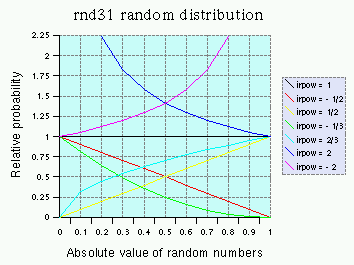
\includegraphics[scale=1]{rnd31_rand} 


 A graph of distributions for different values of irpow.


 \emph{iseed}
 (optional, default=0) -- seed value for random number generator (positive integer in the range 1 to 2147483646 (2 \^{} 31 - 2)). Zero or negative value seeds from current time (this is also the default). Seeding from current time is guaranteed to generate different random sequences, even if multiple random opcodes are called in a very short time. 


  In the a- and k-rate version the seed is set at opcode initialization. With i-rate output, if iseed is zero or negative, it will seed from current time in the first call, and return the next value from the random sequence in successive calls; positive seed values are set at all i-rate calls. The seed is local for a- and k-rate, and global for i-rate units. 


 


\begin{tabular}{cc}
\textbf{Notes}
 \\
� &

 


 
\begin{itemize}
\item 

 although seed values up to 2147483646 are allowed, it is recommended to use smaller numbers ($<$ 1000000) for portability, as large integers may be rounded to a different value if 32-bit floats are used.

\item 

 i-rate \emph{rnd31}
 with a positive seed will always produce the same output value (this is not a bug). To get different values, set seed to 0 in successive calls, which will return the next value from the random sequence.


\end{itemize}


\end{tabular}

\subsection*{Performance}


 \emph{ax}
 -- a-rate output value. 


 \emph{kx}
 -- k-rate output value. 


 \emph{kscl}
 -- output scale. The generated random numbers are in the range -kscl to kscl. It is the same as \emph{iscl}
, but can be varied at k-rate. 


 \emph{krpow}
 -- controls the distribution of random numbers. It is the same as \emph{irpow}
, but can be varied at k-rate. 
\subsection*{Examples}


  Here is an example of the rnd31 opcode at a-rate. It uses the files \emph{rnd31.orc}
 and \emph{rnd31.sco}
. 


 \textbf{Example 1. An example of the rnd31 opcode at a-rate.}

\begin{lstlisting}
/* rnd31.orc */
; Initialize the global variables.
sr = 44100
kr = 4410
ksmps = 10
nchnls = 1

; Instrument #1.
instr 1
  ; Create random numbers at a-rate in the range -2 to 2 with 
  ; a triangular distribution, seed from the current time.
  a31 rnd31 2, -0.5

  ; Use the random numbers to choose a frequency.
  afreq = a31 * 500 + 100

  a1 oscil 30000, afreq, 1
  out a1
endin
/* rnd31.orc */
        
\end{lstlisting}
\begin{lstlisting}
/* rnd31.sco */
; Table #1, a sine wave.
f 1 0 16384 10 1

; Play Instrument #1 for one second.
i 1 0 1
e
/* rnd31.sco */
        
\end{lstlisting}


  Here is an example of the rnd31 opcode at k-rate. It uses the files \emph{rnd31\_krate.orc}
 and \emph{rnd31\_krate.sco}
. 


 \textbf{Example 2. An example of the rnd31 opcode at k-rate.}

\begin{lstlisting}
/* rnd31_krate.orc */
; Initialize the global variables.
sr = 44100
kr = 4410
ksmps = 10
nchnls = 1

; Instrument #1.
instr 1
  ; Create random numbers at k-rate in the range -1 to 1 
  ; with a uniform distribution, seed=10.
  k1 rnd31 1, 0, 10
        
  printks "k1=%f\\n", 0.1, k1
endin
/* rnd31_krate.orc */
        
\end{lstlisting}
\begin{lstlisting}
/* rnd31_krate.sco */
; Play Instrument #1 for one second.
i 1 0 1
e
/* rnd31_krate.sco */
        
\end{lstlisting}
 Its output should include lines like this: \begin{lstlisting}
k1=0.112106
k1=-0.274665
k1=0.403933
      
\end{lstlisting}


  Here is an example of the rnd31 opcode that uses the number 7 as a seed value. It uses the files \emph{rnd31\_seed7.orc}
 and \emph{rnd31\_seed7.sco}
. 


 \textbf{Example 3. An example of the rnd31 opcode that uses the number 7 as a seed value.}

\begin{lstlisting}
/* rnd31_seed7.orc */
; Initialize the global variables.
sr = 44100
kr = 4410
ksmps = 10
nchnls = 1

; Instrument #1.
instr 1
  ; i-rate random numbers with linear distribution, seed=7. 
  ; (Note that the seed was used only in the first call.)
  i1 rnd31 1, 0.5, 7
  i2 rnd31 1, 0.5
  i3 rnd31 1, 0.5
        
  print i1
  print i2
  print i3
endin
/* rnd31_seed7.orc */
        
\end{lstlisting}
\begin{lstlisting}
/* rnd31_seed7.sco */
; Play Instrument #1 for one second.
i 1 0 1
e
/* rnd31_seed7.sco */
        
\end{lstlisting}
 Its output should include lines like this: \begin{lstlisting}
instr 1:  i1 = -0.649
instr 1:  i2 = -0.761
instr 1:  i3 = 0.677
      
\end{lstlisting}


  Here is an example of the rnd31 opcode that uses the current time as a seed value. It uses the files \emph{rnd31\_time.orc}
 and \emph{rnd31\_time.sco}
. 


 \textbf{Example 4. An example of the rnd31 opcode that uses the current time as a seed value.}

\begin{lstlisting}
/* rnd31_time.orc */
; Initialize the global variables.
sr = 44100
kr = 4410
ksmps = 10
nchnls = 1

; Instrument #1.
instr 1
  ; i-rate random numbers with linear distribution,
  ; seeding from the current time. (Note that the seed 
  ; was used only in the first call.)
  i1 rnd31 1, 0.5, 0
  i2 rnd31 1, 0.5
  i3 rnd31 1, 0.5

  print i1
  print i2
  print i3
endin
/* rnd31_time.orc */
        
\end{lstlisting}
\begin{lstlisting}
/* rnd31_time.sco */
; Play Instrument #1 for one second.
i 1 0 1
e
/* rnd31_time.sco */
        
\end{lstlisting}
 Its output should include lines like this: \begin{lstlisting}
instr 1:  i1 = -0.691
instr 1:  i2 = -0.686
instr 1:  i3 = -0.358
      
\end{lstlisting}
\subsection*{Credits}


 Author: Istvan Varga


 New in version 4.16
%\hline 


\begin{comment}
\begin{tabular}{lcr}
Previous &Home &Next \\
rnd &Up &rspline

\end{tabular}


\end{document}
\end{comment}

\newpage
\begin{comment}
\documentclass[10pt]{article}
\usepackage{fullpage, graphicx, url}
\setlength{\parskip}{1ex}
\setlength{\parindent}{0ex}
\title{rspline}
\begin{document}


\begin{tabular}{ccc}
The Alternative Csound Reference Manual & & \\
Previous & &Next

\end{tabular}

%\hline 
\end{comment}
\section{rspline}
rspline�--� Generate random spline curves. \subsection*{Description}


  Generate random spline curves. 
\subsection*{Syntax}


 ar \textbf{rspline}
 xrangeMin, xrangeMax, kcpsMin, kcpsMax


 kr \textbf{rspline}
 krangeMin, krangeMax, kcpsMin, kcpsMax
\subsection*{Performance}


 \emph{kr, ar}
 -- Output signal 


 \emph{xrangeMin, xrangeMax}
 -- Range of values of random-generated points 


 \emph{kcpsMin, kcpsMax}
 -- Range of point-generation rate. Min and max limits are expressed in cps. 


 \emph{xamp}
 -- Amplitude factor 


 \emph{rspline}
 (random-spline-curve generator) is similar to \emph{jspline}
 but output range is defined by means of two limit values. Also in this case, real output range could be a bit greater of range values, because of interpolating curves beetween each pair of random-points. 


  At present time generated curves are quite smooth when cpsMin is not too different from cpsMax. When cpsMin-cpsMax interval is big, some little discontinuity could occurr, but it should not be a problem, in most cases. Maybe the algorithm will be improved in next versions. 


  These opcodes are often better than \emph{jitter}
 when user wants to ``naturalize'' or ``analogize'' digital sounds. They could be used also in algorithmic composition, to generate smooth random melodic lines when used together with \emph{samphold}
 opcode. 


  Note that the result is quite different from the one obtained by filtering white noise, and they allow the user to obtain a much more precise control. 
\subsection*{Credits}


 Author: Gabriel Maldonado


 New in version 4.15
%\hline 


\begin{comment}
\begin{tabular}{lcr}
Previous &Home &Next \\
rnd31 &Up &rtclock

\end{tabular}


\end{document}
\end{comment}

\newpage
\begin{comment}
\documentclass[10pt]{article}
\usepackage{fullpage, graphicx, url}
\setlength{\parskip}{1ex}
\setlength{\parindent}{0ex}
\title{rtclock}
\begin{document}


\begin{tabular}{ccc}
The Alternative Csound Reference Manual & & \\
Previous & &Next

\end{tabular}

%\hline 
\end{comment}
\section{rtclock}
rtclock�--� Read the real time clock from the operating system. \subsection*{Description}


  Read the real-time clock from the operating system. 
\subsection*{Syntax}


 ir \textbf{rtclock}



 kr \textbf{rtclock}

\subsection*{Performance}


  Read the real-time clock from operating system. Under Windows, this changes only once per second. Under GNU/Linux, it ticks every microsecond. Performance under other systems varies. 
\subsection*{Examples}


  Here is an example of the rtclock opcode. It uses the files \emph{rtclock.orc}
 and \emph{rtclock.sco}
. 


 \textbf{Example 1. Example of the rtclock opcode.}

\begin{lstlisting}
/* rtclock.orc */
; Initialize the global variables.
sr = 44100
kr = 44100
ksmps = 1
nchnls = 1

; Instrument #1
instr 1
  ; Get the system time.
  k1 rtclock
  ; Print it once per second.
  printk 1, k1
endin
/* rtclock.orc */
        
\end{lstlisting}
\begin{lstlisting}
/* rtclock.sco */
; Play Instrument #1 for two seconds.
i 1 0 2
e
/* rtclock.sco */
        
\end{lstlisting}
 Its output should include lines like this: \begin{lstlisting}
 i   1 time     0.00002: 1018236096.00000
 i   1 time     1.00002: 1018236224.00000
      
\end{lstlisting}
\subsection*{Credits}


 Author: John ffitch


 Example written by Kevin Conder.


 New in version 4.10
%\hline 


\begin{comment}
\begin{tabular}{lcr}
Previous &Home &Next \\
rspline &Up &s16b14

\end{tabular}


\end{document}
\end{comment}

\newpage
%\begin{comment}
\documentclass[10pt]{article}
\usepackage{fullpage, graphicx, url}
\setlength{\parskip}{1ex}
\setlength{\parindent}{0ex}
\title{s Statement}
\begin{document}


\begin{tabular}{ccc}
The Alternative Csound Reference Manual & & \\
Previous & &Next

\end{tabular}

%\hline 
\end{comment}
\section{s Statement}
s�--� Marks the end of a section. \subsection*{Description}


  The \emph{s statement}
 marks the end of a section. 
\subsection*{Syntax}


 \textbf{s}
 anything
\subsection*{Initialization}


  All p-fields are ignored. 
\subsection*{Performance}


  Sorting of the \emph{i statement}
, \emph{f statement}
 and \emph{a statement}
 by action time is done section by section. 


  Time warping for the \emph{t statement}
 is done section by section. 


  All action times within a section are relative to its beginning. A section statement establishes a new relative time of 0, but has no other reinitializing effects (e.g. stored function tables are preserved across section boundaries). 


  A section is considered complete when all action times and finite durations have been satisfied (i.e., the ``length'' of a section is determined by the last occurring action or turn-off). A section can be extended by the use of an \emph{f0 statement}
. 


  A section ending automatically invokes a Purge of inactive instrument and data spaces. 


 


\begin{tabular}{cc}
\textbf{Note}
 \\
� &

 


 
\begin{itemize}
\item 

  Since score statements are processed section by section, the amount of memory required depends on the maximum number of score statements in a section. Memory allocation is dynamic, and the user will be informed as extra memory blocks are requested during score processing. 

\item 

  For the end of the final section of a score, the \emph{s statement}
 is optional; the \emph{e statement}
 may be used instead. 


\end{itemize}


\end{tabular}

%\hline 
\end{comment}


\begin{comment}
\begin{tabular}{lcr}
Previous &Home &Next \\
r Statement (Repeat Statement) &Up &t Statement (Tempo Statement)

\end{tabular}


\end{document}
\end{comment}

\begin{comment}
\documentclass[10pt]{article}
\usepackage{fullpage, graphicx, url}
\setlength{\parskip}{1ex}
\setlength{\parindent}{0ex}
\title{s16b14}
\begin{document}


\begin{tabular}{ccc}
The Alternative Csound Reference Manual & & \\
Previous & &Next

\end{tabular}

%\hline 
\end{comment}
\section{s16b14}
s16b14�--� Creates a bank of 16 different 14-bit MIDI control message numbers. \subsection*{Description}


  Creates a bank of 16 different 14-bit MIDI control message numbers. 
\subsection*{Syntax}


 i1,...,i16 \textbf{s16b14}
 ichan, ictlno\_msb1, ictlno\_lsb1, imin1, imax1, initvalue1, ifn1,..., ictlno\_msb16, ictlno\_lsb16, imin16, imax16, initvalue16, ifn16


 k1,...,k16 \textbf{s16b14}
 ichan, ictlno\_msb1, ictlno\_lsb1, imin1, imax1, initvalue1, ifn1,..., ictlno\_msb16, ictlno\_lsb16, imin16, imax16, initvalue16, ifn16
\subsection*{Initialization}


 \emph{i1 ... i64}
 -- output values 


 \emph{ichan}
 -- MIDI channel (1-16) 


 \emph{ictlno\_msb1 .... ictlno\_msb32}
 -- MIDI control number, most significant byte (0-127) 


 \emph{ictlno\_lsb1 .... ictlno\_lsb32}
 -- MIDI control number, least significant byte (0-127) 


 \emph{imin1 ... imin64}
 -- minimum values for each controller 


 \emph{imax1 ... imax64}
 -- maximum values for each controller 


 \emph{init1 ... init64}
 -- initial value for each controller 


 \emph{ifn1 ... ifn64}
 -- function table for conversion for each controller 


 \emph{icutoff1 ... icutoff64}
 -- low-pass filter cutoff frequency for each controller 
\subsection*{Performance}


 \emph{k1 ... k64}
 -- output values 


 \emph{s16b14}
 is a bank of MIDI controllers, useful when using MIDI mixer such as Kawai MM-16 or others for changing whatever sound parameter in real-time. The raw MIDI control messages at the input port are converted to agree with \emph{iminN}
 and \emph{imaxN}
, and an initial value can be set. Also, an optional non-interpolated function table with a custom translation curve is allowed, useful for enabling exponential response curves. 


  When no function table translation is required, set the \emph{ifnN}
 value to 0, else set \emph{ifnN}
 to a valid function table number. When table translation is enabled (i.e. setting \emph{ifnN}
 value to a non-zero number referring to an already allocated function table), \emph{initN}
 value should be set equal to \emph{iminN}
 or \emph{imaxN}
 value, else the initial output value will not be the same as specified in \emph{initN}
 argument. 


 \emph{s16b14}
 allows a bank of 16 different MIDI control message numbers. It uses 14-bit values instead of MIDI's normal 7-bit values. 


  As the input and output arguments are many, you can split the line using '$\backslash$' (backslash) character (new in 3.47 version) to improve the readability. Using these opcodes is considerably more efficient than using the separate ones (\emph{ctrl7}
 and \emph{tonek}
) when more controllers are required. 


  In the i-rate version of \emph{s16b14}
, there is not an initial value input argument. The output is taken directly from the current status of internal controller array of Csound. 
\subsection*{Credits}


 


 


\begin{tabular}{ccc}
Author: Gabriel Maldonado &Italy &December 1998

\end{tabular}



 


 New in Csound version 3.50


 Thanks goes to Rasmus Ekman for pointing out the correct MIDI channel and controller number ranges.
%\hline 


\begin{comment}
\begin{tabular}{lcr}
Previous &Home &Next \\
rtclock &Up &s32b14

\end{tabular}


\end{document}
\end{comment}

\newpage
\begin{comment}
\documentclass[10pt]{article}
\usepackage{fullpage, graphicx, url}
\setlength{\parskip}{1ex}
\setlength{\parindent}{0ex}
\title{s32b14}
\begin{document}


\begin{tabular}{ccc}
The Alternative Csound Reference Manual & & \\
Previous & &Next

\end{tabular}

%\hline 
\end{comment}
\section{s32b14}
s32b14�--� Creates a bank of 32 different 14-bit MIDI control message numbers. \subsection*{Description}


  Creates a bank of 32 different 14-bit MIDI control message numbers. 
\subsection*{Syntax}


 i1,...,i32 \textbf{s32b14}
 ichan, ictlno\_msb1, ictlno\_lsb1, imin1, imax1, initvalue1, ifn1,..., ictlno\_msb32, ictlno\_lsb32, imin32, imax32, initvalue32, ifn32


 k1,...,k32 \textbf{s32b14}
 ichan, ictlno\_msb1, ictlno\_lsb1, imin1, imax1, initvalue1, ifn1,..., ictlno\_msb32, ictlno\_lsb32, imin32, imax32, initvalue32, ifn32
\subsection*{Initialization}


 \emph{i1 ... i64}
 -- output values 


 \emph{ichan}
 -- MIDI channel (1-16) 


 \emph{ictlno\_msb1 .... ictlno\_msb32}
 -- MIDI control number, most significant byte (0-127) 


 \emph{ictlno\_lsb1 .... ictlno\_lsb32}
 -- MIDI control number, least significant byte (0-127) 


 \emph{imin1 ... imin64}
 -- minimum values for each controller 


 \emph{imax1 ... imax64}
 -- maximum values for each controller 


 \emph{init1 ... init64}
 -- initial value for each controller 


 \emph{ifn1 ... ifn64}
 -- function table for conversion for each controller 


 \emph{icutoff1 ... icutoff64}
 -- low-pass filter cutoff frequency for each controller 
\subsection*{Performance}


 \emph{k1 ... k64}
 -- output values 


 \emph{s32b14}
 is a bank of MIDI controllers, useful when using MIDI mixer such as Kawai MM-16 or others for changing whatever sound parameter in real-time. The raw MIDI control messages at the input port are converted to agree with \emph{iminN}
 and \emph{imaxN}
, and an initial value can be set. Also, an optional non-interpolated function table with a custom translation curve is allowed, useful for enabling exponential response curves. 


  When no function table translation is required, set the \emph{ifnN}
 value to 0, else set \emph{ifnN}
 to a valid function table number. When table translation is enabled (i.e. setting \emph{ifnN}
 value to a non-zero number referring to an already allocated function table), \emph{initN}
 value should be set equal to \emph{iminN}
 or \emph{imaxN}
 value, else the initial output value will not be the same as specified in \emph{initN}
 argument. 


 \emph{s32b14}
 allows a bank of 32 different MIDI control message numbers. It uses 14-bit values instead of MIDI's normal 7-bit values. 


  As the input and output arguments are many, you can split the line using '$\backslash$' (backslash) character (new in 3.47 version) to improve the readability. Using these opcodes is considerably more efficient than using the separate ones (\emph{ctrl7}
 and \emph{tonek}
) when more controllers are required. 


  In the i-rate version of \emph{s32b14}
, there is not an initial value input argument. The output is taken directly from the current status of internal controller array of Csound. 
\subsection*{Credits}


 


 


\begin{tabular}{ccc}
Author: Gabriel Maldonado &Italy &December 1998

\end{tabular}



 


 New in Csound version 3.50


 Thanks goes to Rasmus Ekman for pointing out the correct MIDI channel and controller number ranges.
%\hline 


\begin{comment}
\begin{tabular}{lcr}
Previous &Home &Next \\
s16b14 &Up &samphold

\end{tabular}


\end{document}
\end{comment}

\newpage
\begin{comment}
\documentclass[10pt]{article}
\usepackage{fullpage, graphicx, url}
\setlength{\parskip}{1ex}
\setlength{\parindent}{0ex}
\title{samphold}
\begin{document}


\begin{tabular}{ccc}
The Alternative Csound Reference Manual & & \\
Previous & &Next

\end{tabular}

%\hline 
\end{comment}
\section{samphold}
samphold�--� Performs a sample-and-hold operation on its input. \subsection*{Description}


  Performs a sample-and-hold operation on its input. 
\subsection*{Syntax}


 ar \textbf{samphold}
 asig, agate [, ival] [, ivstor]


 kr \textbf{samphold}
 ksig, kgate [, ival] [, ivstor]
\subsection*{Initialization}


 \emph{ival, ivstor}
 (optional) -- controls initial disposition of internal save space. If \emph{ivstor}
 is zero the internal ``hold'' value is set to \emph{ival}
 ; else it retains its previous value. Defaults are 0,0 (i.e. init to zero) 
\subsection*{Performance}


 \emph{kgate, xgate}
 -- controls whether to hold the signal. 


 \emph{samphold}
 performs a sample-and-hold operation on its input according to the value of \emph{gate}
. If \emph{gate !- 0}
, the input samples are passed to the output; If \emph{gate = 0}
, the last output value is repeated. The controlling \emph{gate}
 can be a constant, a control signal, or an audio signal. 
\subsection*{Examples}


 


 
\begin{lstlisting}
asrc  \emph{buzz}
      10000,440,20, 1     ; band-limited pulse train
adif  \emph{diff}
      asrc                ; emphasize the highs
anew  \emph{balance}
   adif, asrc          ;   but retain the power
agate \emph{reson}
     asrc,0,440          ; use a lowpass of the original
asamp \emph{samphold}
  anew, agate         ;   to gate the new audiosig
aout  \emph{tone}
      asamp,100           ; smooth out the rough edges
        
\end{lstlisting}


 
\subsection*{See Also}


 \emph{diff}
, \emph{downsamp}
, \emph{integ}
, \emph{interp}
, \emph{upsamp}

%\hline 


\begin{comment}
\begin{tabular}{lcr}
Previous &Home &Next \\
s32b14 &Up &sandpaper

\end{tabular}


\end{document}
\end{comment}

\newpage
\begin{comment}
\documentclass[10pt]{article}
\usepackage{fullpage, graphicx, url}
\setlength{\parskip}{1ex}
\setlength{\parindent}{0ex}
\title{sandpaper}
\begin{document}


\begin{tabular}{ccc}
The Alternative Csound Reference Manual & & \\
Previous & &Next

\end{tabular}

%\hline 
\end{comment}
\section{sandpaper}
sandpaper�--� Semi-physical model of a sandpaper sound. \subsection*{Description}


 \emph{sandpaper}
 is a semi-physical model of a sandpaper sound. It is one of the PhISEM percussion opcodes. PhISEM (Physically Informed Stochastic Event Modeling) is an algorithmic approach for simulating collisions of multiple independent sound producing objects. 
\subsection*{Syntax}


 ar \textbf{sandpaper}
 iamp, idettack [, inum] [, idamp] [, imaxshake]
\subsection*{Initialization}


 \emph{iamp}
 -- Amplitude of output. Note: As these instruments are stochastic, this is only a approximation. 


 \emph{idettack}
 -- period of time over which all sound is stopped 


 \emph{inum}
 (optional) -- The number of beads, teeth, bells, timbrels, etc. If zero, the default value is 128. 


 \emph{idamp}
 (optional) -- the damping factor, as part of this equation: 


 damping\_amount�=�0.998�+�(idamp�*�0.002)


  The default \emph{damping\_amount}
 is 0.999 which means that the default value of \emph{idamp}
 is 0.5. The maximum \emph{damping\_amount}
 is 1.0 (no damping). This means the maximum value for \emph{idamp}
 is 1.0. 


  The recommended range for \emph{idamp}
 is usually below 75\% of the maximum value. 


 \emph{imaxshake}
 (optional) -- amount of energy to add back into the system. The value should be in range 0 to 1. 
\subsection*{Examples}


  Here is an example of the sandpaper opcode. It uses the files \emph{sandpaper.orc}
 and \emph{sandpaper.sco}
. 


 \textbf{Example 1. Example of the sandpaper opcode.}

\begin{lstlisting}
/* sandpaper.orc */
;orchestra ---------------

  sr =           44100
  kr =            4410
  ksmps =              10
  nchnls =               1

instr 01                  ;an example of sandpaper blocks
  a1      line 2, p3, 2                             ;preset amplitude increase
  a2      sandpaper p4, 0.01            ;sandpaper needs a little amp help at these settings
  a3      product a1, a2                               ;increase amplitude
          out a3
          endin
/* sandpaper.orc */
        
\end{lstlisting}
\begin{lstlisting}
/* sandpaper.sco */
;score -------------------

   i1 0 1 26000
   e
/* sandpaper.sco */
        
\end{lstlisting}
\subsection*{See Also}


 \emph{cabasa}
, \emph{crunch}
, \emph{sekere}
, \emph{stix}

\subsection*{Credits}


 


 


\begin{tabular}{cccc}
Author: Perry Cook, part of the PhOLIES (Physically-Oriented Library of Imitated Environmental Sounds) &Adapted by John ffitch &University of Bath, Codemist Ltd. &Bath, UK

\end{tabular}



 


 New in Csound version 4.07


 Added notes by Rasmus Ekman on May 2002.
%\hline 


\begin{comment}
\begin{tabular}{lcr}
Previous &Home &Next \\
samphold &Up &scanhammer

\end{tabular}


\end{document}
\end{comment}

\newpage
\begin{comment}
\documentclass[10pt]{article}
\usepackage{fullpage, graphicx, url}
\setlength{\parskip}{1ex}
\setlength{\parindent}{0ex}
\title{scanhammer}
\begin{document}


\begin{tabular}{ccc}
The Alternative Csound Reference Manual & & \\
Previous & &Next

\end{tabular}

%\hline 
\end{comment}
\section{scanhammer}
scanhammer�--� Copies from one table to another with a gain control. \subsection*{Description}


  This is is a variant of \emph{tablecopy}
, copying from one table to another, starting at \emph{ipos}
, and with a gain control. The number of points copied is determined by the length of the source. Other points are not changed. This opcode can be used to ``hit'' a string in the scanned synthesis code. 
\subsection*{Syntax}


 \textbf{scanhammer}
 isrc, idst, ipos, imult
\subsection*{Initialization}


 \emph{isrc}
 -- source function table. 


 \emph{idst}
 -- destination function table. 


 \emph{ipos}
 -- starting position (in points). 


 \emph{imult}
 -- gain multiplier. A value of 0 will leave values unchanged. 
\subsection*{See Also}


 \emph{scantable}

\subsection*{Credits}


 


 


\begin{tabular}{cc}
Author: Matt Gilliard &April 2002

\end{tabular}



 


 New in version 4.20
%\hline 


\begin{comment}
\begin{tabular}{lcr}
Previous &Home &Next \\
sandpaper &Up &scans

\end{tabular}


\end{document}
\end{comment}

\newpage
\begin{comment}
\documentclass[10pt]{article}
\usepackage{fullpage, graphicx, url}
\setlength{\parskip}{1ex}
\setlength{\parindent}{0ex}
\title{scans}
\begin{document}


\begin{tabular}{ccc}
The Alternative Csound Reference Manual & & \\
Previous & &Next

\end{tabular}

%\hline 
\end{comment}
\section{scans}
scans�--� Generate audio output using scanned synthesis. \subsection*{Description}


  Generate audio output using scanned synthesis. 
\subsection*{Syntax}


 ar \textbf{scans}
 kamp, kfreq, ifn, id [, iorder]
\subsection*{Initialization}


 \emph{ifn}
 -- ftable containing the scanning trajectory. This is a series of numbers that contains addresses of masses. The order of these addresses is used as the scan path. It should not contain values greater than the number of masses, or negative numbers. See the \emph{introduction to the scanned synthesis section}
. 


 \emph{id}
 -- ID number of the \emph{scanu}
 opcode's waveform to use 


 \emph{iorder}
 (optional, default=0) -- order of interpolation used internally. It can take any value in the range 1 to 4, and defaults to 4, which is quartic interpolation. The setting of 2 is quadratic and 1 is linear. The higher numbers are slower, but not necessarily better. 
\subsection*{Performance}


 \emph{kamp}
 -- output amplitude. Note that the resulting amplitude is also dependent on instantaneous value in the wavetable. This number is effectively the scaling factor of the wavetable. 


 \emph{kfreq}
 -- frequency of the scan rate 
\subsection*{Examples}


  Here is an example of the scanned synthesis. It uses the files \emph{scans.orc}
, \emph{scans.sco}
, and \emph{string-128.matrix}
. 


 \textbf{Example 1. Example of the scans opcode.}

\begin{lstlisting}
/* scans.orc */
    sr =   44100
    kr =   4410
    ksmps =   10
    nchnls =   1

    instr 1
a0  = 0
;   scanu init, irate, ifnvel, ifnmass, ifnstif, ifncentr, ifndamp, kmass, kstif, kcentr, kdamp, ileft, iright, kpos, kstrngth, ain, idisp, id
    scanu 1,     .01,    6,       2,       3,     4,        5,       2,     .1,    .1,     -.01,  .1,    .5,     0,    0,        a0,  1,     2
;ar scans kamp,      kfreq,      ifntraj, id
a1  scans ampdb(p4), cpspch(p5), 7,       2
    out a1
    endin
/* scans.orc */
        
\end{lstlisting}
\begin{lstlisting}
/* scans.sco */
; Initial condition
f1 0 128 7 0 64 1 64 0
   
; Masses
f2 0 128 -7 1 128 1
   
; Spring matrices
f3 0 16384 -23 "string-128.matrix"
   
; Centering force
f4  0 128 -7 0 128 2
   
; Damping
f5 0 128 -7 1 128 1
   
; Initial velocity
f6 0 128 -7 0 128 0
   
; Trajectories
f7 0 128 -5 .001 128 128

; Note list
i1 0  10  86 6.00
i1 11 14  86 7.00
i1 15 20  86 5.00
e
/* scans.sco */
        
\end{lstlisting}


  The matrix file ``string-128.matrix'', as well as several other matrices, is also available in a \emph{zipped file}
 from the \emph{Scanned Synthesis page}
 at cSounds.com. 
\subsection*{Credits}


 


 


\begin{tabular}{ccc}
Author: Paris Smaragdis &MIT Media Lab &Boston, Massachussetts USA

\end{tabular}



 


 New in Csound version 4.05
%\hline 


\begin{comment}
\begin{tabular}{lcr}
Previous &Home &Next \\
scanhammer &Up &scantable

\end{tabular}


\end{document}
\end{comment}

\newpage
\begin{comment}
\documentclass[10pt]{article}
\usepackage{fullpage, graphicx, url}
\setlength{\parskip}{1ex}
\setlength{\parindent}{0ex}
\title{scantable}
\begin{document}


\begin{tabular}{ccc}
The Alternative Csound Reference Manual & & \\
Previous & &Next

\end{tabular}

%\hline 
\end{comment}
\section{scantable}
scantable�--� A simpler scanned synthesis implementation. \subsection*{Description}


  A simpler scanned synthesis implementation. This is an implementation of a circular string scanned using external tables. This opcode will allow direct modification and reading of values with the table opcodes. 
\subsection*{Syntax}


 aout \textbf{scantable}
 kamp, kpch, ipos, imass, istiff, idamp, ivel
\subsection*{Initialization}


 \emph{ipos}
 -- table containing position array. 


 \emph{imass}
 -- table containing the mass of the string. 


 \emph{istiff}
 -- table containing the stiffness of the string. 


 \emph{idamp}
 -- table containing the damping factors of the string. 


 \emph{ivel}
 -- table containing the velocities. 
\subsection*{Performance}


 \emph{kamp}
 -- amplitude (gain) of the string. 


 \emph{kpch}
 -- the string's scanned frequency. 
\subsection*{Examples}


  Here is an example of the scantable opcode. It uses the files \emph{scantable.orc}
 and \emph{scantable.sco}
. 


 \textbf{Example 1. Example of the scantable opcode.}

\begin{lstlisting}
/* scantable.orc */
; Initialize the global variables.
sr = 44100
kr = 4410
ksmps = 10
nchnls = 1

; Table #1 - initial position
git1 ftgen 1, 0, 128, 7, 0, 64, 1, 64, 0
; Table #2 - masses
git2 ftgen 2, 0, 128, -7, 1, 128, 1
; Table #3 - stiffness
git3 ftgen 3, 0, 128, -7, 0, 64, 100, 64, 0
; Table #4 - damping
git4 ftgen 4, 0, 128, -7, 1, 128, 1
; Table #5 - initial velocity
git5 ftgen 5, 0, 128, -7, 0, 128, 0

; Instrument #1.
instr 1
  kamp init 20000
  kpch init 220
  ipos = 1
  imass = 2
  istiff = 3
  idamp = 4
  ivel = 5

  a1 scantable kamp, kpch, ipos, imass, istiff, idamp, ivel
  a2 dcblock a1

  out a2
endin
/* scantable.orc */
        
\end{lstlisting}
\begin{lstlisting}
/* scantable.sco */
; Play Instrument #1 for ten seconds.
i 1 0 10
e
/* scantable.sco */
        
\end{lstlisting}
\subsection*{See Also}


 \emph{scanhammer}

\subsection*{Credits}


 


 


\begin{tabular}{cc}
Author: Matt Gilliard &April 2002

\end{tabular}



 


 Example written by Kevin Conder.


 New in version 4.20
%\hline 


\begin{comment}
\begin{tabular}{lcr}
Previous &Home &Next \\
scans &Up &scanu

\end{tabular}


\end{document}
\end{comment}

\newpage
\begin{comment}
\documentclass[10pt]{article}
\usepackage{fullpage, graphicx, url}
\setlength{\parskip}{1ex}
\setlength{\parindent}{0ex}
\title{scanu}
\begin{document}


\begin{tabular}{ccc}
The Alternative Csound Reference Manual & & \\
Previous & &Next

\end{tabular}

%\hline 
\end{comment}
\section{scanu}
scanu�--� Compute the waveform and the wavetable for use in scanned synthesis. \subsection*{Description}


  Compute the waveform and the wavetable for use in scanned synthesis. 
\subsection*{Syntax}


 \textbf{scanu}
 init, irate, ifnvel, ifnmass, ifnstif, ifncentr, ifndamp, kmass, kstif, kcentr, kdamp, ileft, iright, kpos, kstrngth, ain, idisp, id
\subsection*{Initialization}


 \emph{init}
 -- the initial position of the masses. If this is a negative number, then the absolute of \emph{init}
 signifies the table to use as a hammer shape. If \emph{init}
 $>$ 0, the length of it should be the same as the intended mass number, otherwise it can be anything. 


 \emph{ifnvel}
 -- the ftable that contains the initial velocity for each mass. It should have the same size as the intended mass number. 


 \emph{ifnmass}
 -- ftable that contains the mass of each mass. It should have the same size as the intended mass number. 


 \emph{ifnstif}
 -- ftable that contains the spring stiffness of each connection. It should have the same size as the square of the intended mass number. The data ordering is a row after row dump of the connection matrix of the system. 


 \emph{ifncentr}
 -- ftable that contains the centering force of each mass. It should have the same size as the intended mass number. 


 \emph{ifndamp}
 -- the ftable that contains the damping factor of each mass. It should have the same size as the intended mass number. 


 \emph{ileft}
 -- If \emph{init}
 $<$ 0, the position of the left hammer (\emph{ileft}
 = 0 is hit at leftmost, \emph{ileft}
 = 1 is hit at rightmost). 


 \emph{iright}
 -- If \emph{init}
 $<$ 0, the position of the right hammer (\emph{iright}
 = 0 is hit at leftmost, \emph{iright}
 = 1 is hit at rightmost). 


 \emph{idisp}
 -- If 0, no display of the masses is provided. 


 \emph{id}
 -- If positive, the ID of the opcode. This will be used to point the scanning opcode to the proper waveform maker. If this value is negative, the absolute of this value is the wavetable on which to write the waveshape. That wavetable can be used later from an other opcode to generate sound. The initial contents of this table will be destroyed. 
\subsection*{Performance}


 \emph{kmass}
 -- scales the masses 


 \emph{kstif}
 -- scales the spring stiffness 


 \emph{kcentr}
 -- scales the centering force 


 \emph{kdamp}
 -- scales the damping 


 \emph{kpos}
 -- position of an active hammer along the string (\emph{kpos}
 = 0 is leftmost, \emph{kpos}
 = 1 is rightmost). The shape of the hammer is determined by \emph{init}
 and the power it pushes with is \emph{kstrngth}
. 


 \emph{kstrngth}
 -- power that the active hammer uses 


 \emph{ain}
 -- audio input that adds to the velocity of the masses. Amplitude should not be too great. 
\subsection*{Examples}


  For an example, see the documentation on \emph{scans}
. 
\subsection*{Credits}


 


 


\begin{tabular}{cccc}
Author: Paris Smaragdis &MIT Media Lab &Boston, Massachussetts USA &March 2000

\end{tabular}



 


 New in Csound version 4.05
%\hline 


\begin{comment}
\begin{tabular}{lcr}
Previous &Home &Next \\
scantable &Up &schedkwhen

\end{tabular}


\end{document}
\end{comment}

\newpage
\begin{comment}
\documentclass[10pt]{article}
\usepackage{fullpage, graphicx, url}
\setlength{\parskip}{1ex}
\setlength{\parindent}{0ex}
\title{schedkwhen}
\begin{document}


\begin{tabular}{ccc}
The Alternative Csound Reference Manual & & \\
Previous & &Next

\end{tabular}

%\hline 
\end{comment}
\section{schedkwhen}
schedkwhen�--� Adds a new score event generated by a k-rate trigger. \subsection*{Description}


  Adds a new score event generated by a k-rate trigger. 
\subsection*{Syntax}


 \textbf{schedkwhen}
 ktrigger, kmintim, kmaxnum, kinsnum, kwhen, kdur [, ip4] [, ip5] [...]


 \textbf{schedkwhen}
 ktrigger, kmintim, kmaxnum, ``insname'', kwhen, kdur [, ip4] [, ip5] [...]
\subsection*{Initialization}


 \emph{``insname''}
 -- A string (in double-quotes) representing a named instrument. 


 \emph{ip4, ip5, ...}
 -- Equivalent to p4, p5, etc., in a score \emph{i statement}

\subsection*{Performance}


 \emph{ktrigger}
 -- triggers a new score event. If \emph{ktrigger}
 = 0, no new event is triggered. 


 \emph{kmintim}
 -- minimum time between generated events, in seconds. If \emph{kmintim}
 $<$= 0, no time limit exists. If the \emph{kinsnum}
 is negative (to turn off an instrument), this test is bypassed. 


 \emph{kmaxnum}
 -- maximum number of simultaneous instances of instrument \emph{kinsnum}
 allowed. If the number of extant instances of \emph{kinsnum}
 is $>$= \emph{kmaxnum}
, no new event is generated. If \emph{kmaxnum}
 is $<$= 0, it is not used to limit event generation. If the \emph{kinsnum}
 is negative (to turn off an instrument), this test is bypassed. 


 \emph{kinsnum}
 -- instrument number. Equivalent to p1 in a score \emph{i statement}
. 


 \emph{kwhen}
 -- start time of the new event. Equivalent to p2 in a score \emph{i statement}
. Measured from the time of the triggering event. \emph{kwhen}
 must be $>$= 0. If \emph{kwhen}
 $>$ 0, the instrument will not be initialized until the actual time when it should start performing. 


 \emph{kdur}
 -- duration of event. Equivalent to p3 in a score \emph{i statement}
. If \emph{kdur}
 = 0, the instrument will only do an initialization pass, with no performance. If \emph{kdur}
 is negative, a held note is initiated. (See \emph{ihold}
 and \emph{i statement}
.) 


 \emph{Note}
: While waiting for events to be triggered by \emph{schedkwhen}
, the performance must be kept going, or Csound may quit if no score events are expected. To guarantee continued performance, an \emph{f0 statement}
 may be used in the score. 
\subsection*{Examples}


  Here is an example of the schedkwhen opcode. It uses the files \emph{schedkwhen.orc}
 and \emph{schedkwhen.sco}
. 


 \textbf{Example 1. Example of the schedkwhen opcode.}

\begin{lstlisting}
/* schedkwhen.orc */
; Initialize the global variables.
sr = 44100
kr = 44100
ksmps = 1
nchnls = 1

; Instrument #1 - oscillator with a high note.
instr 1
  ; Use the fourth p-field as the trigger.
  ktrigger = p4
  kmintim = 0
  kmaxnum = 2
  kinsnum = 2
  kwhen = 0
  kdur = 0.5

  ; Play Instrument #2 at the same time, if the trigger is set.
  schedkwhen ktrigger, kmintim, kmaxnum, kinsnum, kwhen, kdur

  ; Play a high note.
  a1 oscils 10000, 880, 1
  out a1
endin

; Instrument #2 - oscillator with a low note.
instr 2
  ; Play a low note.
  a1 oscils 10000, 220, 1
  out a1
endin
/* schedkwhen.orc */
        
\end{lstlisting}
\begin{lstlisting}
/* schedkwhen.sco */
; Table #1, a sine wave.
f 1 0 16384 10 1

; p4 = trigger for Instrument #2 (when p4 > 0).
; Play Instrument #1 for half a second, no trigger.
i 1 0 0.5 0
; Play Instrument #1 for half a second, trigger Instrument #2.
i 1 1 0.5 1
e
/* schedkwhen.sco */
        
\end{lstlisting}
\subsection*{Credits}


 


 


\begin{tabular}{cc}
Author: Rasmus Ekman &EMS, Stockholm, Sweden

\end{tabular}



 


 Example written by Kevin Conder.


 New in Csound version 3.59
%\hline 


\begin{comment}
\begin{tabular}{lcr}
Previous &Home &Next \\
scanu &Up &schedkwhennamed

\end{tabular}


\end{document}
\end{comment}

\newpage
\begin{comment}
\documentclass[10pt]{article}
\usepackage{fullpage, graphicx, url}
\setlength{\parskip}{1ex}
\setlength{\parindent}{0ex}
\title{schedkwhennamed}
\begin{document}


\begin{tabular}{ccc}
The Alternative Csound Reference Manual & & \\
Previous & &Next

\end{tabular}

%\hline 
\end{comment}
\section{schedkwhennamed}
schedkwhennamed�--� Similar to schedkwhen but uses a named instrument at init-time. \subsection*{Description}


  Similar to \emph{schedkwhen}
 but uses a named instrument at init-time. 
\subsection*{Syntax}


 \textbf{schedkwhennamed}
 ktrigger, kmintim, kmaxnum, ``name'', kwhen, kdur [, ip4] [, ip5] [...]
\subsection*{Initialization}


 \emph{ip4, ip5, ...}
 -- Equivalent to p4, p5, etc., in a score \emph{i statement}

\subsection*{Performance}


 \emph{ktrigger}
 -- triggers a new score event. If \emph{ktrigger}
 is 0, no new event is triggered. 


 \emph{kmintim}
 -- minimum time between generated events, in seconds. If \emph{kmintim}
 is less than or equal to 0, no time limit exists. 


 \emph{kmaxnum}
 -- maximum number of simultaneous instances of named instrument allowed. If the number of extant instances of the named instrument is greater than or equal to \emph{kmaxnum}
, no new event is generated. If \emph{kmaxnum}
 is less than or equal to 0, it is not used to limit event generation. 


 \emph{``name''}
 -- the named instrument's name. 


 \emph{kwhen}
 -- start time of the new event. Equivalent to p2 in a score \emph{i statement}
. Measured from the time of the triggering event. \emph{kwhen}
 must be greater than or equal to 0. If \emph{kwhen}
 greater than 0, the instrument will not be initialized until the actual time when it should start performing. 


 \emph{kdur}
 -- duration of event. Equivalent to p3 in a score \emph{i statement}
. If \emph{kdur}
 is 0, the instrument will only do an initialization pass, with no performance. If \emph{kdur}
 is negative, a held note is initiated. (See \emph{ihold}
 and \emph{i statement}
.) 


 \emph{Note}
: While waiting for events to be triggered by \emph{schedkwhennamed}
, the performance must be kept going, or Csound may quit if no score events are expected. To guarantee continued performance, an \emph{f0 statement}
 may be used in the score. 
\subsection*{See Also}


 \emph{schedkwhen}

\subsection*{Credits}


 


 


\begin{tabular}{cc}
Author: Rasmus Ekman &EMS, Stockholm, Sweden

\end{tabular}



 


 New in Csound version 4.23
%\hline 


\begin{comment}
\begin{tabular}{lcr}
Previous &Home &Next \\
schedkwhen &Up &schedule

\end{tabular}


\end{document}
\end{comment}

\newpage
\begin{comment}
\documentclass[10pt]{article}
\usepackage{fullpage, graphicx, url}
\setlength{\parskip}{1ex}
\setlength{\parindent}{0ex}
\title{schedule}
\begin{document}


\begin{tabular}{ccc}
The Alternative Csound Reference Manual & & \\
Previous & &Next

\end{tabular}

%\hline 
\end{comment}
\section{schedule}
schedule�--� Adds a new score event. \subsection*{Description}


  Adds a new score event. 
\subsection*{Syntax}


 \textbf{schedule}
 insnum, iwhen, idur [, ip4] [, ip5] [...]


 \textbf{schedule}
 ``insname'', iwhen, idur [, ip4] [, ip5] [...]
\subsection*{Initialization}


 \emph{insnum}
 -- instrument number. Equivalent to p1 in a score \emph{i statement}
. \emph{insnum}
 must be a number greater than the number of the calling instrument. 


 \emph{``insname''}
 -- A string (in double-quotes) representing a named instrument. 


 \emph{iwhen}
 -- start time of the new event. Equivalent to p2 in a score \emph{i statement}
. \emph{iwhen}
 must be nonnegative. If \emph{iwhen}
 is zero, \emph{insum}
 must be greater than or equal to the p1 of the current instrument. 


 \emph{idur}
 -- duration of event. Equivalent to p3 in a score \emph{i statement}
. 


 \emph{ip4, ip5, ...}
 -- Equivalent to p4, p5, etc., in a score \emph{i statement}
. 
\subsection*{Performance}


 \emph{ktrigger}
 -- trigger value for new event 


 \emph{schedule}
 adds a new score event. The arguments, including options, are the same as in a score. The \emph{iwhen}
 time (p2) is measured from the time of this event. 


  If the duration is zero or negative the new event is of MIDI type, and inherits the release sub-event from the scheduling instruction. 
\subsection*{Examples}


  Here is an example of the schedule opcode. It uses the files \emph{schedule.orc}
 and \emph{schedule.sco}
. 


 \textbf{Example 1. Example of the schedule opcode.}

\begin{lstlisting}
/* schedule.orc */
; Initialize the global variables.
sr = 44100
kr = 4410
ksmps = 10
nchnls = 1

; Instrument #1 - oscillator with a high note.
instr 1
  ; Play Instrument #2 at the same time.
  schedule 2, 0, p3

  ; Play a high note.
  a1 oscils 10000, 880, 1
  out a1
endin

; Instrument #2 - oscillator with a low note.
instr 2
  ; Play a low note.
  a1 oscils 10000, 220, 1
  out a1
endin
/* schedule.orc */
        
\end{lstlisting}
\begin{lstlisting}
/* schedule.sco */
; Table #1, a sine wave.
f 1 0 16384 10 1

; Play Instrument #1 for half a second.
i 1 0 0.5
; Play Instrument #1 for half a second.
i 1 1 0.5
e
/* schedule.sco */
        
\end{lstlisting}
\subsection*{See Also}


 \emph{schedwhen}

\subsection*{Credits}


 


 


\begin{tabular}{cccc}
Author: John ffitch &University of Bath/Codemist Ltd. &Bath, UK &November 1998

\end{tabular}



 


 Example written by Kevin Conder.


 New in Csound version 3.491


 Based on work by Gabriel Maldonado


 Thanks goes to David Gladstein, for clarifying the \emph{iwhen}
 parameter.
%\hline 


\begin{comment}
\begin{tabular}{lcr}
Previous &Home &Next \\
schedkwhennamed &Up &schedwhen

\end{tabular}


\end{document}
\end{comment}

\newpage
\begin{comment}
\documentclass[10pt]{article}
\usepackage{fullpage, graphicx, url}
\setlength{\parskip}{1ex}
\setlength{\parindent}{0ex}
\title{schedwhen}
\begin{document}


\begin{tabular}{ccc}
The Alternative Csound Reference Manual & & \\
Previous & &Next

\end{tabular}

%\hline 
\end{comment}
\section{schedwhen}
schedwhen�--� Adds a new score event. \subsection*{Description}


  Adds a new score event. 
\subsection*{Syntax}


 \textbf{schedwhen}
 ktrigger, kinsnum, kwhen, kdur [, ip4] [, ip5] [...]


 \textbf{schedwhen}
 ktrigger, ``insname'', kwhen, kdur [, ip4] [, ip5] [...]
\subsection*{Initialization}


 \emph{ip4, ip5, ...}
 -- Equivalent to p4, p5, etc., in a score \emph{i statement}
. 
\subsection*{Performance}


 \emph{kinsnum}
 -- instrument number. Equivalent to p1 in a score \emph{i statement}
. 


 \emph{``insname''}
 -- A string (in double-quotes) representing a named instrument. 


 \emph{ktrigger}
 -- trigger value for new event 


 \emph{kwhen}
 -- start time of the new event. Equivalent to p2 in a score \emph{i statement}
. 


 \emph{kdur}
 -- duration of event. Equivalent to p3 in a score \emph{i statement}
. 


 \emph{schedwhen}
 adds a new score event. The event is only scheduled when the k-rate value \emph{ktrigger}
 is first non-zero. The arguments, including options, are the same as in a score. The \emph{iwhen}
 time (p2) is measured from the time of this event. 


  If the duration is zero or negative the new event is of MIDI type, and inherits the release sub-event from the scheduling instruction. 


 


\begin{tabular}{cc}
Warning &\textbf{Warning}
 \\
� &

 Support for named instruments is broken in version 4.23


\end{tabular}

\subsection*{Examples}


  Here is an example of the schedwhen opcode. It uses the files \emph{schedwhen.orc}
 and \emph{schedwhen.sco}
. 


 \textbf{Example 1. Example of the schedwhen opcode.}

\begin{lstlisting}
/* schedwhen.orc */
; Initialize the global variables.
sr = 44100
kr = 44100
ksmps = 1
nchnls = 1

; Instrument #1 - oscillator with a high note.
instr 1
  ; Use the fourth p-field as the trigger.
  ktrigger = p4
  kinsnum = 2
  kwhen = 0
  kdur = p3

  ; Play Instrument #2 at the same time, if the trigger is set.
  schedwhen ktrigger, kinsnum, kwhen, kdur

  ; Play a high note.
  a1 oscils 10000, 880, 1
  out a1
endin

; Instrument #2 - oscillator with a low note.
instr 2
  ; Play a low note.
  a1 oscils 10000, 220, 1
  out a1
endin
/* schedwhen.orc */
        
\end{lstlisting}
\begin{lstlisting}
/* schedwhen.sco */
; Table #1, a sine wave.
f 1 0 16384 10 1

; p4 = trigger for Instrument #2 (when p4 > 0).
; Play Instrument #1 for half a second, trigger Instrument #2.
i 1 0 0.5 1
; Play Instrument #1 for half a second, no trigger.
i 1 1 0.5 0
e
/* schedwhen.sco */
        
\end{lstlisting}
\subsection*{See Also}


 \emph{schedule}

\subsection*{Credits}


 


 


\begin{tabular}{cccc}
Author: John ffitch &University of Bath/Codemist Ltd. &Bath, UK &November 1998

\end{tabular}



 


 Example written by Kevin Conder.


 New in Csound version 3.491


 Based on work by Gabriel Maldonado
%\hline 


\begin{comment}
\begin{tabular}{lcr}
Previous &Home &Next \\
schedule &Up &seed

\end{tabular}


\end{document}
\end{comment}

\newpage
%\begin{comment}
\documentclass[10pt]{article}
\usepackage{fullpage, graphicx, url}
\setlength{\parskip}{1ex}
\setlength{\parindent}{0ex}
\title{Amplitude Scaling GEN Routines}
\begin{document}


\begin{tabular}{ccc}
The Alternative Csound Reference Manual & & \\
Previous &The Standard Numeric Score &Next

\end{tabular}

%\hline 
\end{comment}
\section{Amplitude Scaling GEN Routines}


  GEN routines that perform amplitude scaling are \emph{GEN04}
, \emph{GEN12}
, and \emph{GEN24}
. 
%\hline 


\begin{comment}
\begin{tabular}{lcr}
Previous &Home &Next \\
Waveshaping GEN Routines &Up &Mixing GEN Routines

\end{tabular}


\end{document}
\end{comment}

%\begin{comment}
\documentclass[10pt]{article}
\usepackage{fullpage, graphicx, url}
\setlength{\parskip}{1ex}
\setlength{\parindent}{0ex}
\begin{document}
The Alternative Csound Reference Manual Previous The Standard Numeric Score Next \_\_\_\_\_\_\_\_\_\_\_\_\_\_\_\_\_\_\_\_ Evaluation of Expressions In earlier versions of Csound the numbers presented in a score were used as given. There are occasions when some simple evaluation would be easier. This need is increased when there are macros. To assist in this area the syntax of an arithmetic expressions within square brackets [ ] has been introduced. Expressions built from the operations +, -, *, /, \%, and \^{} are allowed, together with grouping with ( ). The expressions can include numbers, and naturally macros whose values are numeric or arithmetic strings. All calculations are made in floating point numbers. Note that unary minus is not yet supported. New in Csound version 3.56 are @ x (next power-of-two greater than or equal to x ) and @@ x (next power-of-two-plus-one greater than or equal to x ). Example r3 CNT i1 0 [0.3*\$CNT.] i1 + [(\$CNT./3)+0.2] e As the three copies of the section have the macro \$CNT. with the different values of 1, 2 and 3, this expands to s i1 0 0.3 i1 0.3 0.533333 s i1 0 0.6 i1 0.6 0.866667 s i1 0 0.9 i1 0.9 1.2 e This is an extreme form, but the evaluation system can be used to ensure that repeated sections are subtly different. Credits Author: John ffitch University of Bath/Codemist Ltd. Bath, UK April, 1998 (New in Csound version 3.48)\_\_\_\_\_\_\_\_\_\_\_\_\_\_\_\_\_\_\_\_\_\_\_\_\_\_\_\_\_\_\_\_\_\_\_\_\_\_\_\_\_\_\_\_\_\_\_\_\_\_\_\_\_\_\_\_\_\_\_\_\_\_\_\_\_\_\_\_\_\_\_\_\_\_\_\_\_\_\_\_\_\_\_\_\_\_ 1 Previous Home Next Multiple File Score Up Score Statements 2 
\end{document}
\end{comment}

%\begin{comment}
\documentclass[10pt]{article}
\usepackage{fullpage, graphicx, url}
\setlength{\parskip}{1ex}
\setlength{\parindent}{0ex}
\title{File Access GEN Routines}
\begin{document}


\begin{tabular}{ccc}
The Alternative Csound Reference Manual & & \\
Previous &The Standard Numeric Score &Next

\end{tabular}

%\hline 
\end{comment}
\section{File Access GEN Routines}


  The GEN routines that access files are \emph{GEN01}
, \emph{GEN23}
, and \emph{GEN28}
. 
%\hline 


\begin{comment}
\begin{tabular}{lcr}
Previous &Home &Next \\
Line/Exponential Segment Generators &Up &Numeric Value Access GEN Routines

\end{tabular}


\end{document}
\end{comment}

%\begin{comment}
\documentclass[10pt]{article}
\usepackage{fullpage, graphicx, url}
\setlength{\parskip}{1ex}
\setlength{\parindent}{0ex}
\title{GEN Routines}
\begin{document}


\begin{tabular}{ccc}
The Alternative Csound Reference Manual & & \\
Previous &Score Statements and GEN Routines &Next

\end{tabular}

%\hline 
\end{comment}
\section{GEN Routines}
\begin{description}
\item[\textbf{Table of Contents}
]\item[GEN01 \&\#8212; Transfers data from a soundfile into a function table. ]\item[GEN02 \&\#8212; Transfers data from immediate pfields into a function table. ]\item[GEN03 \&\#8212; Generates a stored function table by evaluating a polynomial. ]\item[GEN04 \&\#8212; Generates a normalizing function. ]\item[GEN05 \&\#8212; Constructs functions from segments of exponential curves. ]\item[GEN06 \&\#8212; Generates a function comprised of segments of cubic polynomials. ]\item[GEN07 \&\#8212; Constructs functions from segments of straight lines. ]\item[GEN08 \&\#8212; Generate a piecewise cubic spline curve. ]\item[GEN09 \&\#8212; Generate composite waveforms made up of weighted sums of simple sinusoids. ]\item[GEN10 \&\#8212; Generate composite waveforms made up of weighted sums of simple sinusoids. ]\item[GEN11 \&\#8212; Generates an additive set of cosine partials. ]\item[GEN12 \&\#8212; Generates the log of a modified Bessel function of the second kind. ]\item[GEN13 \&\#8212; Stores a polynomial whose coefficients derive from the Chebyshev polynomials of the first kind. ]\item[GEN14 \&\#8212; Stores a polynomial whose coefficients derive from Chebyshevs of the second kind. ]\item[GEN15 \&\#8212; Creates two tables of stored polynomial functions. ]\item[GEN16 \&\#8212; Creates a table from a starting value to an ending value. ]\item[GEN17 \&\#8212; Creates a step function from given x-y pairs. ]\item[GEN18 \&\#8212; Writes composite waveforms made up of pre-existing waveforms. ]\item[GEN19 \&\#8212; Generate composite waveforms made up of weighted sums of simple sinusoids. ]\item[GEN20 \&\#8212; Generates functions of different windows. ]\item[GEN21 \&\#8212; Generates tables of different random distributions. ]\item[GEN22 \&\#8212; Deprecated. ]\item[GEN23 \&\#8212; Reads numeric values from a text file. ]\item[GEN24 \&\#8212; Reads numeric values from another allocated function-table and rescales them. ]\item[GEN25 \&\#8212; Construct functions from segments of exponential curves in breakpoint fashion. ]\item[GEN27 \&\#8212; Construct functions from segments of straight lines in breakpoint fashion. ]\item[GEN28 \&\#8212; Reads a text file which contains a time-tagged trajectory. ]\item[GEN30 \&\#8212; Generates harmonic partials by analyzing an existing table. ]\item[GEN31 \&\#8212; Mixes any waveform specified in an existing table. ]\item[GEN32 \&\#8212; Mixes any waveform, resampled with either FFT or linear interpolation. ]\item[GEN33 \&\#8212; Generate composite waveforms by mixing simple sinusoids. ]\item[GEN34 \&\#8212; Generate composite waveforms by mixing simple sinusoids. ]\item[GEN40 \&\#8212; Generates a random distribution using a distribution histogram. ]\item[GEN41 \&\#8212; Generates a random list of numerical pairs. ]\item[GEN42 \&\#8212; Generates a random distribution of discrete ranges of values. ]
\end{description}
%\hline 


\begin{comment}
\begin{tabular}{lcr}
Previous &Home &Next \\
Score Statements and GEN Routines &Up &GEN01

\end{tabular}


\end{document}
\end{comment}

%\begin{comment}
\documentclass[10pt]{article}
\usepackage{fullpage, graphicx, url}
\setlength{\parskip}{1ex}
\setlength{\parindent}{0ex}
\title{Score Statements and GEN Routines}
\begin{document}


\begin{tabular}{ccc}
The Alternative Csound Reference Manual & & \\
Previous & &Next

\end{tabular}

%\hline 
\end{comment}
\section{Score Statements and GEN Routines}
\section{Score Statements}
\begin{description}
\item[\textbf{Table of Contents}
]\item[a Statement (or Advance Statement) \&\#8212; Advance score time by a specified amount. ]\item[b Statement \&\#8212; This statement resets the clock. ]\item[e Statement \&\#8212; This statement may be used to mark the end of the last section of the score. ]\item[f Statement (or Function Table Statement) \&\#8212; Causes a GEN subroutine to place values in a stored function table. ]\item[i Statement (Instrument or Note Statement) \&\#8212; Makes an instrument active at a specific time and for a certain duration. ]\item[m Statement (Mark Statement) \&\#8212; Sets a named mark in the score. ]\item[n Statement \&\#8212; Repeats a section. ]\item[q Statement \&\#8212; This statement may be used to quiet an instrument. ]\item[r Statement (Repeat Statement) \&\#8212; Starts a repeated section. ]\item[s Statement \&\#8212; Marks the end of a section. ]\item[t Statement (Tempo Statement) \&\#8212; Sets the tempo. ]\item[v Statement \&\#8212; Provides for locally variable time warping of score events. ]\item[x Statement \&\#8212; Skip the rest of the current section. ]
\end{description}
%\hline 


\begin{comment}
\begin{tabular}{lcr}
Previous &Home &Next \\
zkwm &Up &a Statement (or Advance Statement)

\end{tabular}


\end{document}
\end{comment}

%\begin{comment}
\documentclass[10pt]{article}
\usepackage{fullpage, graphicx, url}
\setlength{\parskip}{1ex}
\setlength{\parindent}{0ex}
\title{Score Macros}
\begin{document}


\begin{tabular}{ccc}
The Alternative Csound Reference Manual & & \\
Previous &The Standard Numeric Score &Next

\end{tabular}

%\hline 
\end{comment}
\section{Score Macros}
\subsection*{Description}


  Macros are textual replacements which are made in the score as it is being presented to the system. The macro system in Csound is a very simple one, and uses the characters \# and \$ to define and call macros. This can can allow for simpler score writing, and provide an elementary alternative to full score generation systems.The score macro system is similar to, but independent of, the macro system in the orchestra language. 


 \emph{\#define}
 NAME -- defines a simple macro. The name of the macro must begin with a letter and can consist of any combination of letters and numbers. Case is significant. This form is limiting, in that the variable names are fixed. More flexibility can be obtained by using a macro with arguments, described below. 


 \emph{\#define}
 NAME(\emph{a' b' c'}
) -- defines a macro with arguments. This can be used in more complex situations. The name of the macro must begin with a letter and can consist of any combination of letters and numbers. Within the replacement text, the arguments can be substituted by the form: \$A. In fact, the implementation defines the arguments as simple macros. There may be up to 5 arguments, and the names may be any choice of letters. Remember that case is significant in macro names. 


 \emph{\$NAME.}
 -- calls a defined macro. To use a macro, the name is used following a \$ character. The name is terminated by the first character which is neither a letter nor a number. If it is necessary for the name not to terminate with a space, a period, which will be ignored, can be used to terminate the name. The string, \emph{\$NAME}
., is replaced by the replacement text from the definition. The replacement text can also include macro calls. 


 \emph{\#undef}
 NAME -- undefines a macro name. If a macro is no longer required, it can be undefined with \emph{\#undef}
 NAME. 
\subsection*{Syntax}


 \textbf{\#define}
 NAME \# replacement text \#


 \textbf{\#define}
 NAME(a' b' c') \# replacement text \#


 \textbf{\$NAME.}



 \textbf{\#undef}
 NAME
\subsection*{Initialization}


 \emph{\# replacement text \#}
 -- The replacement text is any character string (not containing a \#) and can extend over mutliple lines. The replacement text is enclosed within the \# characters, which ensure that additional characters are not inadvertently captured. 
\subsection*{Performance}


  Some care is needed with textual replacement macros, as they can sometimes do strange things. They take no notice of any meaning, so spaces are significant. This is why, unlike the C programming language, the definition has the replacement text surrounded by \# characters. Used carefully, this simple macro system is a powerful concept, but it can be abused. 


 \textbf{Another Use For Macros. }
 When writing a complex score it is sometimes all too easy to forget to what the various instrument numbers refer. One can use macros to give names to the numbers. For example 


 
\begin{lstlisting}
\emph{#define}
 Flute  #i1#
\emph{#define}
 Whoop  #i2#

\emph{$Flute.}
  0  10  4000  440
\emph{$Whoop.}
  5  1
          
\end{lstlisting}


 
\subsection*{Examples}


 


 \textbf{Example 1. Simple Macro}



  A note-event has a set of p-fields which are repeated: \begin{lstlisting}
\emph{#define}
 ARGS # 1.01 2.33 138#
i1 0 1 8.00  1000 $ARGS
i1 0 1 8.01  1500 $ARGS
i1 0 1 8.02  1200 $ARGS
i1 0 1 8.03  1000 $ARGS
          
\end{lstlisting}
 This will get expanded before sorting into: \begin{lstlisting}
i1 0 1 8.00  1000 1.01 2.33 138
i1 0 1 8.01  1500 1.01 2.33 138
i1 0 1 8.02  1200 1.01 2.33 138
i1 0 1 8.03  1000 1.01 2.33 138
          
\end{lstlisting}



  This can save typing, and is makes revisions easier. If there were two sets of p-fields one could have a second macro (there is no real limit on the number of macros one can define). 


 
\begin{lstlisting}
\emph{#define}
 ARGS1 # 1.01 2.33 138#
\emph{#define}
 ARGS2 # 1.41 10.33 1.00#
i1 0 1 8.00  1000 $ARGS1
i1 0 1 8.01  1500 $ARGS2
i1 0 1 8.02  1200 $ARGS1
i1 0 1 8.03  1000 $ARGS2
        
\end{lstlisting}


 


 


 \textbf{Example 2. Macros with arguments}



 


 
\begin{lstlisting}
\emph{#define}
 ARG(A) # 2.345   1.03   $A   234.9#
i1 0 1 8.00 1000 $ARG(2.0)
i1  + 1 8.01 1200 $ARG(3.0)
            
\end{lstlisting}


 
 which expands to 

 
\begin{lstlisting}
i1 0 1 8.00 1000 2.345   1.03   2.0   234.9
i1  + 1 8.01 1200 2.345   1.03   3.0   234.9
            
\end{lstlisting}


 
\subsection*{Credits}


 Author: John ffitch


 University of Bath/Codemist Ltd.


 Bath, UK


 April, 1998 (New in Csound version 3.48)
%\hline 


\begin{comment}
\begin{tabular}{lcr}
Previous &Home &Next \\
Ramping &Up &Multiple File Score

\end{tabular}


\end{document}
\end{comment}

%\begin{comment}
\documentclass[10pt]{article}
\usepackage{fullpage, graphicx, url}
\setlength{\parskip}{1ex}
\setlength{\parindent}{0ex}
\title{Mixing GEN Routines}
\begin{document}


\begin{tabular}{ccc}
The Alternative Csound Reference Manual & & \\
Previous &The Standard Numeric Score &Next

\end{tabular}

%\hline 
\end{comment}
\section{Mixing GEN Routines}


  GEN routines that mix together waverforms are \emph{GEN18}
, \emph{GEN31}
, and \emph{GEN32}
. 
%\hline 


\begin{comment}
\begin{tabular}{lcr}
Previous &Home &Next \\
Amplitude Scaling GEN Routines &Up &Reference

\end{tabular}


\end{document}
\end{comment}

%\begin{comment}
\documentclass[10pt]{article}
\usepackage{fullpage, graphicx, url}
\setlength{\parskip}{1ex}
\setlength{\parindent}{0ex}
\title{Next-P and Previous-P Symbols}
\begin{document}


\begin{tabular}{ccc}
The Alternative Csound Reference Manual & & \\
Previous &The Standard Numeric Score &Next

\end{tabular}

%\hline 
\end{comment}
\section{Next-P and Previous-P Symbols}


  At the close of any of the operations \emph{Carry}
, \emph{Tempo}
, and \emph{Sort}
, three additional score features are interpreted during file writeout: next-p, previous-p, and \emph{ramping}
. 


 \emph{i statement}
 pfields containing the symbols \emph{np}
\emph{x}
 or \emph{pp}
\emph{x}
 (where \emph{x}
 is some integer) will be replaced by the appropriate pfield value found on the next i statement (or previous i statement) that has the same p1. For example, the symbol \emph{np}
7 will be replaced by the value found in p7 of the next note that is to be played by this instrument. \emph{np}
 and \emph{pp }
symbols are recursive and can reference other \emph{np}
 and \emph{pp}
 symbols which can reference others, etc. References must eventually terminate in a real number or a \emph{ramp symbol}
. Closed loop references should be avoided. \emph{np}
 and \emph{pp}
 symbols are illegal in p1, p2 and p3 (although they may reference these). \emph{np}
 and \emph{pp}
 symbols may be Carried. \emph{np}
 and \emph{pp}
 references cannot cross a Section boundary. Any forward or backward reference to a non-existent note-statement will be given the value zero. 


  E.g.: the statements 


 
\begin{lstlisting}
i1   0    1    10   np4  pp5 
i1   1    1    20
i1   1    1    30
     
\end{lstlisting}


 
 will result in 

 
\begin{lstlisting}
  i1   0    1    10   20   0 
  i1   1    1    20   30   20 
  i1   2    1    30   0    30
     
\end{lstlisting}


 


 \emph{np}
 and \emph{pp}
 symbols can provide an instrument with contextual knowledge of the score, enabling it to glissando or crescendo, for instance, toward the pitch or dynamic of some future event (which may or may not be immediately adjacent). Note that while the \emph{Carry}
 feature will propagate \emph{np}
 and \emph{pp}
 through unsorted statements, the operation that interprets these symbols is acting on a time-warped and fully sorted version of the score. 
%\hline 


\begin{comment}
\begin{tabular}{lcr}
Previous &Home &Next \\
The Standard Numeric Score &Up &Ramping

\end{tabular}


\end{document}
\end{comment}

%\begin{comment}
\documentclass[10pt]{article}
\usepackage{fullpage, graphicx, url}
\setlength{\parskip}{1ex}
\setlength{\parindent}{0ex}
\title{Numeric Value Access GEN Routines}
\begin{document}


\begin{tabular}{ccc}
The Alternative Csound Reference Manual & & \\
Previous &The Standard Numeric Score &Next

\end{tabular}

%\hline 
\end{comment}
\section{Numeric Value Access GEN Routines}


  The GEN routines that generate tables from numeric values are \emph{GEN02}
 and \emph{GEN17}
. 
%\hline 


\begin{comment}
\begin{tabular}{lcr}
Previous &Home &Next \\
File Access GEN Routines &Up &Window Function GEN Routines

\end{tabular}


\end{document}
\end{comment}

%\begin{comment}
\documentclass[10pt]{article}
\usepackage{fullpage, graphicx, url}
\setlength{\parskip}{1ex}
\setlength{\parindent}{0ex}
\title{Ramping}
\begin{document}


\begin{tabular}{ccc}
The Alternative Csound Reference Manual & & \\
Previous &The Standard Numeric Score &Next

\end{tabular}

%\hline 
\end{comment}
\section{Ramping}


 \emph{i statement}
 pfields containing the symbol \emph{$<$}
 will be replaced by values derived from linear interpolation of a time-based ramp. Ramps are anchored at each end by the first real number found in the same pfield of a preceding and following note played by the same instrument. E.g.: the statements 


 
\begin{lstlisting}
i1   0    1    100
i1   1    1    <
i1   2    1    <
i1   3    1    400
i1   4    1    <
i1   5    1    0
      
\end{lstlisting}


 
 will result in 

 
\begin{lstlisting}
i1   0    1    100 
i1   1    1    200
i1   2    1    300
i1   3    1    400
i1   4    1    200
i1   5    1    0
      
\end{lstlisting}


 


  Ramps cannot cross a Section boundary. Ramps cannot be anchored by an \emph{np}
 or \emph{pp}
 symbol (although they may be referenced by these). Ramp symbols are illegal in p1, p2 and p3. Ramp symbols may be Carried. Note, however, that while the Carry feature will propagate ramp symbols through unsorted statements, the operation that interprets these symbols is acting on a time-warped and fully sorted version of the score. In fact, time-based linear interpolation is based on warped score-time, so that a ramp which spans a group of accelerating notes will remain linear with respect to strict chronological time. 


  Starting with Csound version 3.52, using the symbols ( or ) will result in an exponential interpolation ramp, similar to \emph{expon}
. The symbols \{ and \} to define an exponential ramp have been deprecated. Using the symbol \&\#732; will result in uniform, random distribution between the first and last values of the ramp. Use of these functions must follow the same rules as the linear ramp function. 
%\hline 


\begin{comment}
\begin{tabular}{lcr}
Previous &Home &Next \\
Next-P and Previous-P Symbols &Up &Score Macros

\end{tabular}


\end{document}
\end{comment}

%\begin{comment}
\documentclass[10pt]{article}
\usepackage{fullpage, graphicx, url}
\setlength{\parskip}{1ex}
\setlength{\parindent}{0ex}
\title{Random Function GEN Routines}
\begin{document}


\begin{tabular}{ccc}
The Alternative Csound Reference Manual & & \\
Previous &The Standard Numeric Score &Next

\end{tabular}

%\hline 
\end{comment}
\section{Random Function GEN Routines}


  GEN routines the generate random distributions are \emph{GEN21}
, \emph{GEN40}
, \emph{GEN41}
, and \emph{GEN42}
. 
%\hline 


\begin{comment}
\begin{tabular}{lcr}
Previous &Home &Next \\
Window Function GEN Routines &Up &Waveshaping GEN Routines

\end{tabular}


\end{document}
\end{comment}

%\begin{comment}
\documentclass[10pt]{article}
\usepackage{fullpage, graphicx, url}
\setlength{\parskip}{1ex}
\setlength{\parindent}{0ex}
\title{Line/Exponential Segment Generators}
\begin{document}


\begin{tabular}{ccc}
The Alternative Csound Reference Manual & & \\
Previous &The Standard Numeric Score &Next

\end{tabular}

%\hline 
\end{comment}
\section{Line/Exponential Segment Generators}


  GEN routines that generate tables with linear or exponential segments are \emph{GEN05}
, \emph{GEN06}
, \emph{GEN07}
, \emph{GEN08}
, \emph{GEN16}
, \emph{GEN25}
, and \emph{GEN27}
. 
%\hline 


\begin{comment}
\begin{tabular}{lcr}
Previous &Home &Next \\
Sine/Cosine Generators &Up &File Access GEN Routines

\end{tabular}


\end{document}
\end{comment}

%\begin{comment}
\documentclass[10pt]{article}
\usepackage{fullpage, graphicx, url}
\setlength{\parskip}{1ex}
\setlength{\parindent}{0ex}
\title{Sine/Cosine Generators}
\begin{document}


\begin{tabular}{ccc}
The Alternative Csound Reference Manual & & \\
Previous &The Standard Numeric Score &Next

\end{tabular}

%\hline 
\end{comment}
\section{Sine/Cosine Generators}


  The GEN routines that generate sine or cosine values are \emph{GEN09}
, \emph{GEN10}
, \emph{GEN11}
, \emph{GEN19}
, \emph{GEN30}
, \emph{GEN33}
, and \emph{GEN34}
. 
%\hline 


\begin{comment}
\begin{tabular}{lcr}
Previous &Home &Next \\
Score Statements &Up &Line/Exponential Segment Generators

\end{tabular}


\end{document}
\end{comment}

%\begin{comment}
\documentclass[10pt]{article}
\usepackage{fullpage, graphicx, url}
\setlength{\parskip}{1ex}
\setlength{\parindent}{0ex}
\title{Score Statements}
\begin{document}


\begin{tabular}{ccc}
The Alternative Csound Reference Manual & & \\
Previous &The Standard Numeric Score &Next

\end{tabular}

%\hline 
\end{comment}
\section{Score Statements}


  The statements used in scores are \emph{a}
, \emph{b}
, \emph{e}
, \emph{f}
, \emph{i}
, \emph{m}
, \emph{n}
, \emph{r}
, \emph{s}
, \emph{t}
, \emph{v}
, and \emph{x}
. 
%\hline 


\begin{comment}
\begin{tabular}{lcr}
Previous &Home &Next \\
Evaluation of Expressions &Up &Sine/Cosine Generators

\end{tabular}


\end{document}
\end{comment}

%\begin{comment}
\documentclass[10pt]{article}
\usepackage{fullpage, graphicx, url}
\setlength{\parskip}{1ex}
\setlength{\parindent}{0ex}
\title{The Standard Numeric Score}
\begin{document}


\begin{tabular}{ccc}
The Alternative Csound Reference Manual & & \\
Previous & &Next

\end{tabular}

%\hline 
\end{comment}
\section{The Standard Numeric Score}
\section{Preprocessing of Standard Scores}


  A \emph{Score}
 (a collection of score statements) is divided into time-ordered sections by the \emph{s statement}
. Before being read by the orchestra, a score is preprocessed one section at a time. Each section is normally processed by 3 routines: \emph{Carry}
, \emph{Tempo}
, and \emph{Sort}
. 
\subsection*{Carry}


  Within a group of consecutive \emph{i statements}
 whose p1 whole numbers correspond, any pfield left empty will take its value from the same pfield of the preceding statement. An empty pfield can be denoted by a single point (.) delimited by spaces. No point is required after the last nonempty pfield. The output of Carry preprocessing will show the carried values explicitly. The Carry Feature is not affected by intervening comments or blank lines; it is turned off only by a non- \emph{i statement}
 or by an \emph{i statement}
 with unlike p1 whole number. 


  Three additional features are available for p2 alone: +, \^{} + \emph{x}
, and \^{} - \emph{x}
. The symbol + in p2 will be given the value of p2 + p3 from the preceding i statement. This enables note action times to be automatically determined from the sum of preceding durations. The + symbol can itself be carried. It is legal only in p2. E.g.: the statements 


 
\begin{lstlisting}
i1   0    .5        100         
i .  +                   
i
        
\end{lstlisting}


 
 will result in 

 
\begin{lstlisting}
i1   0         .5        100
i1   .5        .5        100
i1   1         .5        100
        
\end{lstlisting}


 


  The symbols \^{} + \emph{x}
 and \^{} - \emph{x}
 determine the current p2 by adding or subtracting, respectively, the value of \emph{x}
 from the preceding p2. These may be used in p2 only. 


  The Carry feature should be used liberally. Its use, especially in large scores, can greatly reduce input typing and will simplify later changes. 
\subsection*{Tempo}


  This operation time warps a score section according to the information in a \emph{t statement}
. The tempo operation converts p2 (and, for \emph{i statements}
, p3) from original beats into real seconds, since those are the units required by the orchestra. After time warping, score files will be seen to have orchestra-readable format demonstrated by the following: \emph{i}
 p1 p2beats p2seconds p3beats p3seconds p4 p5 .... 
\subsection*{Sort}


  This routine sorts all action-time statements into chronological order by p2 value. It also sorts coincident events into precedence order. Whenever an \emph{f statement}
 and an \emph{i statement}
 have the same p2 value, the \emph{f statement}
 will precede. Whenever two or more \emph{i statements}
 have the same p2 value, they will be sorted into ascending p1 value order. If they also have the same p1 value, they will be sorted into ascending p3 value order. Score sorting is done section by section (see \emph{s statement}
). Automatic sorting implies that score statements may appear in any order within a section. 
\subsection*{N.B.}


  The operations Carry, Tempo and Sort are combined in a 3-phase single pass over a score file, to produce a new file in orchestra-readable format ( see the Tempo example). Processing can be invoked either explicitly by the \emph{Scsort}
 command, or implicitly by CSound which processes the score before calling the orchestra. Source-format files and orchestra-readable files are both in ASCII character form, and may be either perused or further modified by standard text editors. User-written routines can be used to modify score files before or after the above processes, provided the final orchestra-readable statement format is not violated. Sections of different formats can be sequentially batched; and sections of like format can be merged for automatic sorting. 
%\hline 


\begin{comment}
\begin{tabular}{lcr}
Previous &Home &Next \\
Zak Patch System &Up &Next-P and Previous-P Symbols

\end{tabular}


\end{document}
\end{comment}

%\begin{comment}
\documentclass[10pt]{article}
\usepackage{fullpage, graphicx, url}
\setlength{\parskip}{1ex}
\setlength{\parindent}{0ex}
\title{Waveshaping GEN Routines}
\begin{document}


\begin{tabular}{ccc}
The Alternative Csound Reference Manual & & \\
Previous &The Standard Numeric Score &Next

\end{tabular}

%\hline 
\end{comment}
\section{Waveshaping GEN Routines}


  The GEN routines that have waveshaping functionality are \emph{GEN03}
, \emph{GEN13}
, \emph{GEN14}
, and \emph{GEN15}
. 
%\hline 


\begin{comment}
\begin{tabular}{lcr}
Previous &Home &Next \\
Random Function GEN Routines &Up &Amplitude Scaling GEN Routines

\end{tabular}


\end{document}
\end{comment}

%\begin{comment}
\documentclass[10pt]{article}
\usepackage{fullpage, graphicx, url}
\setlength{\parskip}{1ex}
\setlength{\parindent}{0ex}
\title{Window Function GEN Routines}
\begin{document}


\begin{tabular}{ccc}
The Alternative Csound Reference Manual & & \\
Previous &The Standard Numeric Score &Next

\end{tabular}

%\hline 
\end{comment}
\section{Window Function GEN Routines}


  The GEN routine for window functions is \emph{GEN20}
. 
%\hline 


\begin{comment}
\begin{tabular}{lcr}
Previous &Home &Next \\
Numeric Value Access GEN Routines &Up &Random Function GEN Routines

\end{tabular}


\end{document}
\end{comment}

\begin{comment}
\documentclass[10pt]{article}
\usepackage{fullpage, graphicx, url}
\setlength{\parskip}{1ex}
\setlength{\parindent}{0ex}
\title{sdif2ad}
\begin{document}


\begin{tabular}{ccc}
The Alternative Csound Reference Manual & & \\
Previous & &Next

\end{tabular}

%\hline 
\end{comment}
\section{sdif2ad}
sdif2ad�--� Converts SDIF files to files usable by adsynt. \subsection*{Description}


  Convert files Sound Description Interchange Format (SDIF) to the format usable by Csound's \emph{adsyn}
 opcode. As of Csound version 4.10, \emph{sdif2ad}
 was available only as a standalone program for Windows console and DOS. 
\subsection*{Syntax}


 \textbf{Csound -U sdif2ad}
 [flags] infilename outfilename
\subsection*{Initialization}


  Flags: 


 
\begin{itemize}
\item 

 \emph{-s}
N -- apply amplitude scale factor N

\item 

 \emph{-p}
N -- keep only the first N partials. Limited to 1024 partials. The source partial track indices are used directly to select internal storage. As these can be arbitrary values, the maximum of 1024 partials may not be realized in all cases.

\item 

 \emph{-r}
 -- byte-reverse output file data. The byte-reverse option is there to facilitate transfer across platforms, as Csound's \emph{adsyn}
 file format is not portable.


\end{itemize}


  If the filename passed to \emph{hetro}
 has the extension ``.sdif'', data will be written in SDIF format as 1TRC frames of additive synthesis data. The utility program \emph{sdif2ad}
 can be used to convert any SDIF file containing a stream of 1TRC data to the Csound \emph{adsyn}
 format. \emph{sdif2ad}
 allows the user to limit the number of partials retained, and to apply an amplitude scaling factor. This is often necessary, as the SDIF specification does not, as of the release of \emph{sdif2ad}
, require amplitudes to be within a particular range. \emph{sdif2ad}
 reports information about the file to the console, including the frequency range. 


  The main advantages of SDIF over the \emph{adsyn}
 format, for Csound users, is that SDIF files are fully portable across platforms (data is ``big-endian''), and do not have the duration limit of 32.76 seconds imposed by the 16 bit \emph{adsyn}
 format. This limit is necessarily imposed by \emph{sdif2ad}
. Eventually, SDIF reading will be incorporated directly into \emph{adsyn}
, thus enabling files of any length (subject to system memory limits) to be analysed and processed. 


  Users should remember that the SDIF formats are still under development. While the 1TRC format is now fairly well established, it can still change. 


  For detailed information on the Sound Description Interchange Format, refer to the CNMAT website: \emph{\url{http://cnmat.CNMAT.Berkeley.EDU/SDIF}}



  Some other SDIF resources (including a viewer) are available via the NC\_DREAM website: \emph{\url{http://www.bath.ac.uk/~masjpf/NCD/dreamhome.html}}

\subsection*{Credits}


 Author: Richard Dobson


 Somerset, England


 August, 2000


 New in Csound version 4.08
%\hline 


\begin{comment}
\begin{tabular}{lcr}
Previous &Home &Next \\
pvlook &Up &srconv

\end{tabular}


\end{document}
\end{comment}

\newpage
\begin{comment}
\documentclass[10pt]{article}
\usepackage{fullpage, graphicx, url}
\setlength{\parskip}{1ex}
\setlength{\parindent}{0ex}
\title{seed}
\begin{document}


\begin{tabular}{ccc}
The Alternative Csound Reference Manual & & \\
Previous & &Next

\end{tabular}

%\hline 
\end{comment}
\section{seed}
seed�--� Sets the global seed value. \subsection*{Description}


  Sets the global seed value for all \emph{x-class noise generators}
, as well as other opcodes that use a random call, such as \emph{grain}
. \emph{rand}
, \emph{randi}
, \emph{randh}
, \emph{rnd}
(x), and \emph{birnd}
(x) are not affected by seed. 
\subsection*{Syntax}


 \textbf{seed}
 ival
\subsection*{Performance}


  Use of \emph{seed}
 will provide predictable results from an orchestra using with random generators, when required from multiple performances. 


  When specifying a seed value, \emph{ival}
 should be an integer between 0 and 232. If \emph{ival}
 = 0, the value of \emph{ival}
 will be derived from the system clock. 
%\hline 


\begin{comment}
\begin{tabular}{lcr}
Previous &Home &Next \\
schedwhen &Up &sekere

\end{tabular}


\end{document}
\end{comment}

\newpage
\begin{comment}
\documentclass[10pt]{article}
\usepackage{fullpage, graphicx, url}
\setlength{\parskip}{1ex}
\setlength{\parindent}{0ex}
\title{sekere}
\begin{document}


\begin{tabular}{ccc}
The Alternative Csound Reference Manual & & \\
Previous & &Next

\end{tabular}

%\hline 
\end{comment}
\section{sekere}
sekere�--� Semi-physical model of a sekere sound. \subsection*{Description}


 \emph{sekere}
 is a semi-physical model of a sekere sound. It is one of the PhISEM percussion opcodes. PhISEM (Physically Informed Stochastic Event Modeling) is an algorithmic approach for simulating collisions of multiple independent sound producing objects. 
\subsection*{Syntax}


 ar \textbf{sekere}
 iamp, idettack [, inum] [, idamp] [, imaxshake]
\subsection*{Initialization}


 \emph{iamp}
 -- Amplitude of output. Note: As these instruments are stochastic, this is only a approximation. 


 \emph{idettack}
 -- period of time over which all sound is stopped 


 \emph{inum}
 (optional) -- The number of beads, teeth, bells, timbrels, etc. If zero, the default value is 64. 


 \emph{idamp}
 (optional) -- the damping factor, as part of this equation: 


 damping\_amount�=�0.998�+�(idamp�*�0.002)


  The default \emph{damping\_amount}
 is 0.999 which means that the default value of \emph{idamp}
 is 0.5. The maximum \emph{damping\_amount}
 is 1.0 (no damping). This means the maximum value for \emph{idamp}
 is 1.0. 


  The recommended range for \emph{idamp}
 is usually below 75\% of the maximum value. 


 \emph{imaxshake}
 (optional) -- amount of energy to add back into the system. The value should be in range 0 to 1. 
\subsection*{Examples}


  Here is an example of the sekere opcode. It uses the files \emph{sekere.orc}
 and \emph{sekere.sco}
. 


 \textbf{Example 1. Example of the sekere opcode.}

\begin{lstlisting}
/* sekere.orc */
;orchestra ---------------

  sr =           44100
  kr =            4410
  ksmps =              10
  nchnls =               1

instr 01                  ;an example of a sekere
a1      sekere p4, 0.01
          out a1
          endin
/* sekere.orc */
        
\end{lstlisting}
\begin{lstlisting}
/* sekere.sco */
;score -------------------

   i1 0 1 26000
   e
/* sekere.sco */
        
\end{lstlisting}
\subsection*{See Also}


 \emph{cabasa}
, \emph{crunch}
, \emph{sandpaper}
, \emph{stix}

\subsection*{Credits}


 


 


\begin{tabular}{cccc}
Author: Perry Cook, part of the PhISEM (Physically Informed Stochastic Event Modeling) &Adapted by John ffitch &University of Bath, Codemist Ltd. &Bath, UK

\end{tabular}



 


 New in Csound version 4.07


 Added notes by Rasmus Ekman on May 2002.
%\hline 


\begin{comment}
\begin{tabular}{lcr}
Previous &Home &Next \\
seed &Up &semitone

\end{tabular}


\end{document}
\end{comment}

\newpage
\begin{comment}
\documentclass[10pt]{article}
\usepackage{fullpage, graphicx, url}
\setlength{\parskip}{1ex}
\setlength{\parindent}{0ex}
\title{semitone}
\begin{document}


\begin{tabular}{ccc}
The Alternative Csound Reference Manual & & \\
Previous & &Next

\end{tabular}

%\hline 
\end{comment}
\section{semitone}
semitone�--� Calculates a factor to raise/lower a frequency by a given amount of semitones. \subsection*{Description}


  Calculates a factor to raise/lower a frequency by a given amount of semitones. 
\subsection*{Syntax}


 \textbf{semitone}
(x)


  This function works at a-rate, i-rate, and k-rate. 
\subsection*{Initialization}


 \emph{x}
 -- a value expressed in semitones. 
\subsection*{Performance}


  The value returned by the \emph{semitone}
 function is a factor. You can multiply a frequency by this factor to raise/lower it by the given amount of semitones. 
\subsection*{Examples}


  Here is an example of the semitone opcode. It uses the files \emph{semitone.orc}
 and \emph{semitone.sco}
. 


 \textbf{Example 1. Example of the semitone opcode.}

\begin{lstlisting}
/* semitone.orc */
; Initialize the global variables.
sr = 44100
kr = 4410
ksmps = 10
nchnls = 1

; Instrument #1.
instr 1
  ; The root note is A above middle-C (440 Hz)
  iroot = 440

  ; Raise the root note by three semitones to C.
  isemitone = 3

  ; Calculate the new note.
  ifactor = semitone(isemitone)
  inew = iroot * ifactor

  ; Print out all of the values.
  print iroot
  print ifactor
  print inew
endin
/* semitone.orc */
        
\end{lstlisting}
\begin{lstlisting}
/* semitone.sco */
; Play Instrument #1 for one second.
i 1 0 1
e
/* semitone.sco */
        
\end{lstlisting}
 Its output should include lines like: \begin{lstlisting}
instr 1:  iroot = 440.000
instr 1:  ifactor = 1.189
instr 1:  inew = 523.229
      
\end{lstlisting}
\subsection*{See Also}


 \emph{cent}
, \emph{db}
, \emph{octave}

\subsection*{Credits}


 Example written by Kevin Conder.


 New in version 4.16
%\hline 


\begin{comment}
\begin{tabular}{lcr}
Previous &Home &Next \\
sekere &Up &sense

\end{tabular}


\end{document}
\end{comment}

\newpage
\begin{comment}
\documentclass[10pt]{article}
\usepackage{fullpage, graphicx, url}
\setlength{\parskip}{1ex}
\setlength{\parindent}{0ex}
\title{sense}
\begin{document}


\begin{tabular}{ccc}
The Alternative Csound Reference Manual & & \\
Previous & &Next

\end{tabular}

%\hline 
\end{comment}
\section{sense}
sense�--� Same as the sensekey opcode. \subsection*{Description}


  Same as the \emph{sensekey}
 opcode. 
\subsection*{Syntax}


 kr \textbf{sense}

%\hline 


\begin{comment}
\begin{tabular}{lcr}
Previous &Home &Next \\
semitone &Up &sensekey

\end{tabular}


\end{document}
\end{comment}

\newpage
\begin{comment}
\documentclass[10pt]{article}
\usepackage{fullpage, graphicx, url}
\setlength{\parskip}{1ex}
\setlength{\parindent}{0ex}
\title{sensekey}
\begin{document}


\begin{tabular}{ccc}
The Alternative Csound Reference Manual & & \\
Previous & &Next

\end{tabular}

%\hline 
\end{comment}
\section{sensekey}
sensekey�--� Returns the ASCII code of a key that has been pressed. \subsection*{Description}


  Returns the ASCII code of a key that has been pressed, or -1 if no key has been pressed. 
\subsection*{Syntax}


 kr \textbf{sensekey}

\subsection*{Performance}


  At release, this has not been properly verified, and seems not to work at all on Windows. 


 


\begin{tabular}{cc}
\textbf{Note}
 \\
� &

  This opcode can also be written as \emph{sense}
. 


\end{tabular}

\subsection*{Examples}


  Here is an example of the sensekey opcode. It uses the files \emph{sensekey.orc}
 and \emph{sensekey.sco}
. 


 \textbf{Example 1. Example of the sensekey opcode.}

\begin{lstlisting}
/* sensekey.orc */
; Initialize the global variables.
sr = 44100
kr = 4410
ksmps = 10
nchnls = 1

; Instrument #1.
instr 1
  k1 sensekey
  printk2 k1
endin
/* sensekey.orc */
        
\end{lstlisting}
\begin{lstlisting}
/* sensekey.sco */
; Play Instrument #1 for thirty seconds.
i 1 0 30
e
/* sensekey.sco */
        
\end{lstlisting}
 Here is what the output should look like when the ``q'' button is pressed... \begin{lstlisting}
q i1 357967744.00000
      
\end{lstlisting}
\subsection*{Credits}


 


 


\begin{tabular}{cccc}
Author: John ffitch &University of Bath, Codemist. Ltd. &Bath, UK &October 2000

\end{tabular}



 


 Example written by Kevin Conder.


 New in Csound version 4.09. Renamed in Csound version 4.10.
%\hline 


\begin{comment}
\begin{tabular}{lcr}
Previous &Home &Next \\
sense &Up &seqtime

\end{tabular}


\end{document}
\end{comment}

\newpage
\begin{comment}
\documentclass[10pt]{article}
\usepackage{fullpage, graphicx, url}
\setlength{\parskip}{1ex}
\setlength{\parindent}{0ex}
\title{seqtime}
\begin{document}


\begin{tabular}{ccc}
The Alternative Csound Reference Manual & & \\
Previous & &Next

\end{tabular}

%\hline 
\end{comment}
\section{seqtime}
seqtime�--� Generates a trigger signal according to the values stored in a table. \subsection*{Description}


  Generates a trigger signal according to the values stored in a table. 
\subsection*{Syntax}


 ktrig\_out \textbf{seqtime}
 ktime\_unit, kstart, kloop, kinitndx, kfn\_times
\subsection*{Performance}


 \emph{ktrig\_out}
 -- output trigger signal 


 \emph{ktime\_unit}
 -- unit of measure of time, related to seconds. 


 \emph{kstart}
 -- start index of looped section 


 \emph{kloop}
 -- end index of looped section 


 \emph{kinitndx}
 -- initial index 


 


\begin{tabular}{cc}
\textbf{Note}
 \\
� &

  Although \emph{kinitndx}
 is listed as k-rate, it is in fact accessed only at init-time. So if you are using a k-rate argument, it must be assigned with \emph{init}
. 


\end{tabular}



 \emph{kfn\_times}
 -- number of table containing a sequence of times 


  This opcode handles timed-sequences of groups of values stored into a table. 


 \emph{seqtime}
 generates a trigger signal (a sequence of impulses, see also \emph{trigger}
 opcode), according to the values stored in the \emph{kfn\_times}
 table. This table should contain a series of delta-times (i.e. times beetween to adjacent events). The time units stored into table are expressed in seconds, but can be rescaled by means of ktime\_unit argument. The table can be filled with \emph{GEN02}
 or by means of an external text-file containing numbers, with \emph{GEN23}
. 


  It is possible to start the sequence from a value different than the first, by assigning to \emph{initndx}
 an index different than zero (which corresponds to the first value of the table). Normally the sequence is looped, and the start and end of loop can be adjusted by modifying \emph{kstart}
 and \emph{kloop}
 arguments. User must be sure that values of these arguments (as well as \emph{initndx}
) correspond to valid table numbers, otherwise Csound will crash (because no range-checking is implementeted). 


  It is possible to disable loop (one-shot mode) by assigning the same value both to \emph{kstart}
 and \emph{kloop}
 arguments. In this case, the last read element will be the one corresponding to the value of such arguments. Table can be read backward by assigning a negative \emph{kloop}
 value. It is possible to trigger two events almost at the same time (actually separated by a k-cycle) by giving a zero value to the corresponding delta-time. First element contained in the table should be zero, if the user intends to send a trigger impulse, it should come immediately after the orchestra instrument containing \emph{seqtime}
 opcode. 
\subsection*{Examples}


 


 \textbf{Example 1. Example of the seqtime opcode.}

\begin{lstlisting}
        instr   1
icps    cpsmidi
iamp    ampmidi 5000
ktrig   seqtime 1,       1,          10,      0,   1
trigseq ktrig, 0, 10, 0, 2, kdur, kampratio, kfreqratio
        schedkwhen      ktrig, -1, -1, 2, 0, kdur, kampratio*iamp, kfreqratio*icps
        endin


        instr  2
**** put here your intrument code *******
        out     a1
        endin
        
\end{lstlisting}
\subsection*{See Also}


 \emph{GEN02}
, \emph{GEN23}
, \emph{trigseq}

\subsection*{Credits}


 Author: Gabriel Maldonado


 November 2002. Added a note about the \emph{kinitndx}
 parameter, thanks to Rasmus Ekman.


 New in version 4.06
%\hline 


\begin{comment}
\begin{tabular}{lcr}
Previous &Home &Next \\
sensekey &Up &setctrl

\end{tabular}


\end{document}
\end{comment}

\newpage
\begin{comment}
\documentclass[10pt]{article}
\usepackage{fullpage, graphicx, url}
\setlength{\parskip}{1ex}
\setlength{\parindent}{0ex}
\title{setctrl}
\begin{document}


\begin{tabular}{ccc}
The Alternative Csound Reference Manual & & \\
Previous & &Next

\end{tabular}

%\hline 
\end{comment}
\section{setctrl}
setctrl�--� Configurable slider controls for realtime user input. \subsection*{Description}


  Configurable slider controls for realtime user input. Requires Winsound or TCL/TK. \emph{setctrl}
 sets a slider to a specific value, or sets a minimum or maximum range. 
\subsection*{Syntax}


 \textbf{setctrl}
 inum, ival, itype
\subsection*{Initialization}


 \emph{inum}
 -- number of the slider to set 


 \emph{ival}
 -- value to be sent to the slider 


 \emph{itype}
 -- type of value sent to the slider as follows: 


 
\begin{itemize}
\item 

 1 -- set the current value. Initial value is 0.

\item 

 2 -- set the minimum value. Default is 0.

\item 

 3 -- set the maximum value. Default is 127.

\item 

 4 -- set the label. (New in Csound version 4.09)


\end{itemize}
\subsection*{Performance}


  Calling \emph{setctrl}
 will create a new slider on the screen. There is no theoretical limit to the number of sliders. Windows and TCL/TK use only integers for slider values, so the values may need rescaling. GUIs usually pass values at a fairly slow rate, so it may be advisable to pass the output of control through \emph{port}
. 
\subsection*{Examples}


  Here is an example of the setctrl opcode. It uses the files \emph{setctrl.orc}
 and \emph{setctrl.sco}
. 


 \textbf{Example 1. Example of the setctrl opcode.}

\begin{lstlisting}
/* setctrl.orc */
; Initialize the global variables.
sr = 44100
kr = 4410
ksmps = 10
nchnls = 1

; Instrument #1.
instr 1
  ; Display the label "Volume" on Slider #1.
  setctrl 1, "Volume", 4
  ; Set Slider #1's initial value to 20.
  setctrl 1, 20, 1
  
  ; Capture and display the values for Slider #1.
  k1 control 1
  printk2 k1

  ; Play a simple oscillator.
  ; Use the values from Slider #1 for amplitude.
  kamp = k1 * 128
  a1 oscil kamp, 440, 1
  out a1
endin
/* setctrl.orc */
        
\end{lstlisting}
\begin{lstlisting}
/* setsctrl.sco */
; Table #1, a sine wave.
f 1 0 16384 10 1

; Play Instrument #1 for thirty seconds.
i 1 0 30
e
/* setsctrl.sco */
        
\end{lstlisting}
 Its output should include lines like this: \begin{lstlisting}
 i1    38.00000
 i1    40.00000
 i1    43.00000
      
\end{lstlisting}
\subsection*{See Also}


 \emph{control}

\subsection*{Credits}


 


 


\begin{tabular}{cccc}
Author: John ffitch &University of Bath, Codemist. Ltd. &Bath, UK &May 2000

\end{tabular}



 


 Example written by Kevin Conder.


 New in Csound version 4.06
%\hline 


\begin{comment}
\begin{tabular}{lcr}
Previous &Home &Next \\
seqtime &Up &setksmps

\end{tabular}


\end{document}
\end{comment}

\newpage
\begin{comment}
\documentclass[10pt]{article}
\usepackage{fullpage, graphicx, url}
\setlength{\parskip}{1ex}
\setlength{\parindent}{0ex}
\title{setksmps}
\begin{document}


\begin{tabular}{ccc}
The Alternative Csound Reference Manual & & \\
Previous & &Next

\end{tabular}

%\hline 
\end{comment}
\section{setksmps}
setksmps�--� Sets the local ksmps value in a user-defined opcode block. \subsection*{Description}


  Sets the local ksmps value in a user-defined opcode block. 


  The \emph{setksmps}
 statement can be used to set the local \emph{ksmps}
 value of the user-defined opcode block. It has one i-time parameter specifying the new \emph{ksmps}
 value (which is left unchanged if zero is used). \emph{setksmps}
 should be used before any other opcodes (but allowed after \emph{xin}
), otherwise unpredictable results may occur. 
\subsection*{Syntax}


 \textbf{setksmps}
 iksmps
\subsection*{Initialization}


 \emph{iksmps}
 -- sets the local ksmps value. 


  If \emph{iksmps}
 is set to zero, the \emph{ksmps}
 of the caller instrument or opcode is used (this is the default behavior). 


 


\begin{tabular}{cc}
\textbf{Note}
 \\
� &

  The local \emph{ksmps}
 is implemented by splitting up a control period into smaller sub-kperiods and temporarily modifying internal Csound global variables. This also requires converting the rate of k-rate input and output arguments (input variables receive the same value in all sub-kperiods, while outputs are written only in the last one). 


\end{tabular}



 


\begin{tabular}{cc}
Warning &\textbf{Warning about local ksmps}
 \\
� &

  When the local \emph{ksmps}
 is not the same as the orchestra level \emph{ksmps}
 value (as specified in the orchestra header). Global a-rate operations must not be used in the user-defined opcode block. 


  These include: 


 
\begin{itemize}
\item 

 any access to ``ga'' variables

\item 

 a-rate zak opcodes (\emph{zar}
, \emph{zaw}
, etc.)

\item 

 \emph{tablera}
 and \emph{tablewa}
 (these two opcodes may in fact work, but caution is needed)

\item 

 The \emph{in}
 and \emph{out}
 opcode family (these read from, and write to global a-rate buffers)


\end{itemize}


  In general, the local \emph{ksmps}
 should be used with care as it is an experimental feature. Though it works correctly in most cases. 


\end{tabular}



  The \emph{setksmps}
 statement can be used to set the local \emph{ksmps}
 value of the user-defined opcode block. It has one i-time parameter specifying the new \emph{ksmps}
 value (which is left unchanged if zero is used). \emph{setksmps}
 should be used before any other opcodes (but allowed after \emph{xin}
), otherwise unpredictable results may occur. 
\subsection*{Performance}


  The syntax of a user-defined opcode block is as follows: 


 opcode��name,�outtypes,�intypes\\ 
 xinarg1�[,�xinarg2]�[,�xinarg3]�...�[xinargN]��xin\\ 
 [setksmps��iksmps]\\ 
 ...�the�rest�of�the�instrument's�code.\\ 
 xout��xoutarg1�[,�xoutarg2]�[,�xoutarg3]�...�[xoutargN]\\ 
 endop\\ 
 ������


  The new opcode can then be used with the usual syntax: 


 [xinarg1]�[,�xinarg2]�...�[xinargN]��name��[xoutarg1]�[,�xoutarg2]�...�[xoutargN]�[,�iksmps]\\ 
 ������
\subsection*{Examples}


  See the example for the \emph{opcode}
 opcode. 
\subsection*{See Also}


 \emph{endop}
, \emph{opcode}
, \emph{xin}
, \emph{xout}

\subsection*{Credits}


 Author: Istvan Varga, 2002; based on code by Matt J. Ingalls


 New in version 4.22
%\hline 


\begin{comment}
\begin{tabular}{lcr}
Previous &Home &Next \\
setctrl &Up &sfilist

\end{tabular}


\end{document}
\end{comment}

\newpage
\begin{comment}
\documentclass[10pt]{article}
\usepackage{fullpage, graphicx, url}
\setlength{\parskip}{1ex}
\setlength{\parindent}{0ex}
\title{sfilist}
\begin{document}


\begin{tabular}{ccc}
The Alternative Csound Reference Manual & & \\
Previous & &Next

\end{tabular}

%\hline 
\end{comment}
\section{sfilist}
sfilist�--� Prints a list of all instruments of a previously loaded SoundFont2 (SF2) file. \subsection*{Description}


  Prints a list of all instruments of a previously loaded SoundFont2 (SF2) sample file. These opcodes allow management the sample-structure of SF2 files. In order to understand the usage of these opcodes, the user must have some knowledge of the SF2 format, so a brief description of this format can be found in the \emph{SoundFont2 File Format Appendix}
. 
\subsection*{Syntax}


 \textbf{sfilist}
 ifilhandle
\subsection*{Initialization}


 \emph{ifilhandle}
 -- unique number generated by \emph{sfload}
 opcode to be used as an identifier for a SF2 file. Several SF2 files can be loaded and activated at the same time. 
\subsection*{Performance}


 \emph{sfilist}
 prints a list of all instruments of a previously loaded SF2 file to the console. 


  These opcodes only support the sample structure of SF2 files. The modulator structure of the SoundFont2 format is not supported in Csound. Any modulation or processing to the sample data is left to the Csound user, bypassing all restrictions forced by the SF2 standard. 
\subsection*{See Also}


 \emph{sfinstr}
, \emph{sfinstrm}
, \emph{sfload}
, \emph{sfpassign}
, \emph{sfplay}
, \emph{sfplaym}
, \emph{sfplist}
, \emph{sfpreset}

\subsection*{Credits}


 


 


\begin{tabular}{ccc}
Author: Gabriel Maldonado &Italy &May 2000

\end{tabular}



 


 New in Csound Version 4.07
%\hline 


\begin{comment}
\begin{tabular}{lcr}
Previous &Home &Next \\
setksmps &Up &sfinstr

\end{tabular}


\end{document}
\end{comment}

\newpage
\begin{comment}
\documentclass[10pt]{article}
\usepackage{fullpage, graphicx, url}
\setlength{\parskip}{1ex}
\setlength{\parindent}{0ex}
\title{sfinstr}
\begin{document}


\begin{tabular}{ccc}
The Alternative Csound Reference Manual & & \\
Previous & &Next

\end{tabular}

%\hline 
\end{comment}
\section{sfinstr}
sfinstr�--� Plays a SoundFont2 (SF2) sample instrument, generating a stereo sound. \subsection*{Description}


  Plays a SoundFont2 (SF2) sample instrument, generating a stereo sound. These opcodes allow management the sample-structure of SF2 files. In order to understand the usage of these opcodes, the user must have some knowledge of the SF2 format, so a brief description of this format can be found in the \emph{SoundFont2 File Format Appendix}
. 
\subsection*{Syntax}


 ar1, ar2 \textbf{sfinstr}
 ivel, inotenum, xamp, xfreq, instrnum, ifilhandle [, iflag] [, ioffset]
\subsection*{Initialization}


 \emph{ivel}
 -- velocity value 


 \emph{inotenum}
 -- MIDI note number value 


 \emph{instrnum}
 -- number of an instrument of a SF2 file. 


 \emph{ifilhandle}
 -- unique number generated by \emph{sfload}
 opcode to be used as an identifier for a SF2 file. Several SF2 files can be loaded and activated at the same time. 


 \emph{iflag}
 (optional) -- flag regarding the behavior of \emph{xfreq}
 and \emph{inotenum}



 \emph{ioffset}
 (optional) -- start playing at offset, in samples. 
\subsection*{Performance}


 \emph{xamp}
 -- amplitude correction factor 


 \emph{xfreq}
 -- frequency value or frequency multiplier, depending by \emph{iflag}
. When \emph{iflag}
 = 0, \emph{xfreq}
 is a multiplier of a the default frequency, assigned by SF2 preset to the \emph{inotenum}
 value. When \emph{iflag}
 = 1, \emph{xfreq}
 is the absolute frequency of the output sound, in Hz. Default is 0. 


  When \emph{iflag}
 = 0, \emph{inotenum}
 sets the frequency of the output according to the MIDI note number used, and \emph{xfreq}
 is used as a multiplier. When \emph{iflag}
 = 1, the frequency of the output, is set directly by \emph{xfreq}
. This allows the user to use any kind of micro-tuning based scales. However, this method is designed to work correctly only with presets tuned to the default equal temperament. Attempts to use this method with a preset already having non-standard tunings, or with drum-kit-based presets, could give unexpected results. 


  Adjustment of the amplitude can be done by varying the \emph{xamp}
 argument, which acts as a multiplier. 


  The \emph{ioffset}
 parameter allows the sound to start from a sample different than the first one. The user should make sure that its value is within the length of the specific sound. Otherwise, Csound will probably crash. 


 \emph{sfinstr}
 plays an SF2 instrument instead of a preset (an SF2 instrument is the base of a preset layer). \emph{instrnum}
 specifies the instrument number, and the user must be sure that the specified number belongs to an existing instrument of a determinate soundfont bank. Notice that both \emph{xamp}
 and \emph{xfreq}
 can operate at k-rate as well as a-rate, but both arguments must work at the same rate. 


  These opcodes only support the sample structure of SF2 files. The modulator structure of the SoundFont2 format is not supported in Csound. Any modulation or processing to the sample data is left to the Csound user, bypassing all restrictions forced by the SF2 standard. 
\subsection*{See Also}


 \emph{sfilist}
, \emph{sfinstrm}
, \emph{sfload}
, \emph{sfpassign}
, \emph{sfplay}
, \emph{sfplaym}
, \emph{sfplist}
, \emph{sfpreset}

\subsection*{Credits}


 


 


\begin{tabular}{ccc}
Author: Gabriel Maldonado &Italy &May 2000

\end{tabular}



 


 New in Csound Version 4.07
%\hline 


\begin{comment}
\begin{tabular}{lcr}
Previous &Home &Next \\
sfilist &Up &sfinstr3

\end{tabular}


\end{document}
\end{comment}

\newpage
\begin{comment}
\documentclass[10pt]{article}
\usepackage{fullpage, graphicx, url}
\setlength{\parskip}{1ex}
\setlength{\parindent}{0ex}
\title{sfinstr3}
\begin{document}


\begin{tabular}{ccc}
The Alternative Csound Reference Manual & & \\
Previous & &Next

\end{tabular}

%\hline 
\end{comment}
\section{sfinstr3}
sfinstr3�--� Plays a SoundFont2 (SF2) sample instrument, generating a stereo sound with cubic interpolation. \subsection*{Description}


  Plays a SoundFont2 (SF2) sample instrument, generating a stereo sound with cubic interpolation. These opcodes allow management the sample-structure of SF2 files. In order to understand the usage of these opcodes, the user must have some knowledge of the SF2 format, so a brief description of this format can be found in the \emph{SoundFont2 File Format Appendix}
. 
\subsection*{Syntax}


 ar1, ar2 \textbf{sfinstr3}
 ivel, inotenum, xamp, xfreq, instrnum, ifilhandle [, iflag] [, ioffset]
\subsection*{Initialization}


 \emph{ivel}
 -- velocity value 


 \emph{inotenum}
 -- MIDI note number value 


 \emph{instrnum}
 -- number of an instrument of a SF2 file. 


 \emph{ifilhandle}
 -- unique number generated by \emph{sfload}
 opcode to be used as an identifier for a SF2 file. Several SF2 files can be loaded and activated at the same time. 


 \emph{iflag}
 (optional) -- flag regarding the behavior of \emph{xfreq}
 and \emph{inotenum}



 \emph{ioffset}
 (optional) -- start playing at offset, in samples. 
\subsection*{Performance}


 \emph{xamp}
 -- amplitude correction factor 


 \emph{xfreq}
 -- frequency value or frequency multiplier, depending by \emph{iflag}
. When \emph{iflag}
 = 0, \emph{xfreq}
 is a multiplier of a the default frequency, assigned by SF2 preset to the \emph{inotenum}
 value. When \emph{iflag}
 = 1, \emph{xfreq}
 is the absolute frequency of the output sound, in Hz. Default is 0. 


  When \emph{iflag}
 = 0, \emph{inotenum}
 sets the frequency of the output according to the MIDI note number used, and \emph{xfreq}
 is used as a multiplier. When \emph{iflag}
 = 1, the frequency of the output, is set directly by \emph{xfreq}
. This allows the user to use any kind of micro-tuning based scales. However, this method is designed to work correctly only with presets tuned to the default equal temperament. Attempts to use this method with a preset already having non-standard tunings, or with drum-kit-based presets, could give unexpected results. 


  Adjustment of the amplitude can be done by varying the \emph{xamp}
 argument, which acts as a multiplier. 


  The \emph{ioffset}
 parameter allows the sound to start from a sample different than the first one. The user should make sure that its value is within the length of the specific sound. Otherwise, Csound will probably crash. 


 \emph{sfinstr3}
 is a cubic-interpolation version of \emph{sfinstr}
. Difference of sound-quality is noticeable specially in bass-frequency-transposed samples. In high-freq-transposed samples the difference is less noticeable, and I suggest to use linear-interpolation versions, because they are faster. 


  These opcodes only support the sample structure of SF2 files. The modulator structure of the SoundFont2 format is not supported in Csound. Any modulation or processing to the sample data is left to the Csound user, bypassing all restrictions forced by the SF2 standard. 
\subsection*{See Also}


 \emph{sfilist}
, \emph{sfinstr3m}
, \emph{sfinstrm}
, \emph{sfinstr}
, \emph{sfload}
, \emph{sfpassign}
, \emph{sfplay3}
, \emph{sfplay3m}
, \emph{sfplay}
, \emph{sfplaym}
, \emph{sfplist}
, \emph{sfpreset}

\subsection*{Credits}


 


 


\begin{tabular}{ccc}
Author: Gabriel Maldonado &Italy &May 2000

\end{tabular}



 


 New in Csound Version 4.07
%\hline 


\begin{comment}
\begin{tabular}{lcr}
Previous &Home &Next \\
sfinstr &Up &sfinstr3m

\end{tabular}


\end{document}
\end{comment}

\newpage
\begin{comment}
\documentclass[10pt]{article}
\usepackage{fullpage, graphicx, url}
\setlength{\parskip}{1ex}
\setlength{\parindent}{0ex}
\title{sfinstr3m}
\begin{document}


\begin{tabular}{ccc}
The Alternative Csound Reference Manual & & \\
Previous & &Next

\end{tabular}

%\hline 
\end{comment}
\section{sfinstr3m}
sfinstr3m�--� Plays a SoundFont2 (SF2) sample instrument, generating a mono sound with cubic interpolation. \subsection*{Description}


  Plays a SoundFont2 (SF2) sample instrument, generating a mono sound with cubic interpolation. These opcodes allow management the sample-structure of SF2 files. In order to understand the usage of these opcodes, the user must have some knowledge of the SF2 format, so a brief description of this format can be found in the \emph{SoundFont2 File Format Appendix}
. 
\subsection*{Syntax}


 ar \textbf{sfinstr3m}
 ivel, inotenum, xamp, xfreq, instrnum, ifilhandle [, iflag] [, ioffset]
\subsection*{Initialization}


 \emph{ivel}
 -- velocity value 


 \emph{inotenum}
 -- MIDI note number value 


 \emph{instrnum}
 -- number of an instrument of a SF2 file. 


 \emph{ifilhandle}
 -- unique number generated by \emph{sfload}
 opcode to be used as an identifier for a SF2 file. Several SF2 files can be loaded and activated at the same time. 


 \emph{iflag}
 (optional) -- flag regarding the behavior of \emph{xfreq}
 and \emph{inotenum}



 \emph{ioffset}
 (optional) -- start playing at offset, in samples. 
\subsection*{Performance}


 \emph{xamp}
 -- amplitude correction factor 


 \emph{xfreq}
 -- frequency value or frequency multiplier, depending by \emph{iflag}
. When \emph{iflag}
 = 0, \emph{xfreq}
 is a multiplier of a the default frequency, assigned by SF2 preset to the \emph{inotenum}
 value. When \emph{iflag}
 = 1, \emph{xfreq}
 is the absolute frequency of the output sound, in Hz. Default is 0. 


  When \emph{iflag}
 = 0, \emph{inotenum}
 sets the frequency of the output according to the MIDI note number used, and \emph{xfreq}
 is used as a multiplier. When \emph{iflag}
 = 1, the frequency of the output, is set directly by \emph{xfreq}
. This allows the user to use any kind of micro-tuning based scales. However, this method is designed to work correctly only with presets tuned to the default equal temperament. Attempts to use this method with a preset already having non-standard tunings, or with drum-kit-based presets, could give unexpected results. 


  Adjustment of the amplitude can be done by varying the \emph{xamp}
 argument, which acts as a multiplier. 


  The \emph{ioffset}
 parameter allows the sound to start from a sample different than the first one. The user should make sure that its value is within the length of the specific sound. Otherwise, Csound will probably crash. 


 \emph{sfinstr3m}
 is a cubic-interpolation version of \emph{sfinstrm}
. Difference of sound-quality is noticeable specially in bass-frequency-transposed samples. In high-freq-transposed samples the difference is less noticeable, and I suggest to use linear-interpolation versions, because they are faster. 


  These opcodes only support the sample structure of SF2 files. The modulator structure of the SoundFont2 format is not supported in Csound. Any modulation or processing to the sample data is left to the Csound user, bypassing all restrictions forced by the SF2 standard. 
\subsection*{See Also}


 \emph{sfilist}
, \emph{sfinstr3}
, \emph{sfinstr}
, \emph{sfinstrm}
, \emph{sfload}
, \emph{sfpassign}
, \emph{sfplay3}
, \emph{sfplay3m}
, \emph{sfplay}
, \emph{sfplaym}
, \emph{sfplist}
, \emph{sfpreset}

\subsection*{Credits}


 


 


\begin{tabular}{ccc}
Author: Gabriel Maldonado &Italy &May 2000

\end{tabular}



 


 New in Csound Version 4.07
%\hline 


\begin{comment}
\begin{tabular}{lcr}
Previous &Home &Next \\
sfinstr3 &Up &sfinstrm

\end{tabular}


\end{document}
\end{comment}

\newpage
\begin{comment}
\documentclass[10pt]{article}
\usepackage{fullpage, graphicx, url}
\setlength{\parskip}{1ex}
\setlength{\parindent}{0ex}
\title{sfinstrm}
\begin{document}


\begin{tabular}{ccc}
The Alternative Csound Reference Manual & & \\
Previous & &Next

\end{tabular}

%\hline 
\end{comment}
\section{sfinstrm}
sfinstrm�--� Plays a SoundFont2 (SF2) sample instrument, generating a mono sound. \subsection*{Description}


  Plays a SoundFont2 (SF2) sample instrument, generating a mono sound. These opcodes allow management the sample-structure of SF2 files. In order to understand the usage of these opcodes, the user must have some knowledge of the SF2 format, so a brief description of this format can be found in the \emph{SoundFont2 File Format Appendix}
. 
\subsection*{Syntax}


 ar \textbf{sfinstrm}
 ivel, inotenum, xamp, xfreq, instrnum, ifilhandle [, iflag] [, ioffset]
\subsection*{Initialization}


 \emph{ivel}
 -- velocity value 


 \emph{inotenum}
 -- MIDI note number value 


 \emph{instrnum}
 -- number of an instrument of a SF2 file. 


 \emph{ifilhandle}
 -- unique number generated by \emph{sfload}
 opcode to be used as an identifier for a SF2 file. Several SF2 files can be loaded and activated at the same time. 


 \emph{iflag}
 (optional) -- flag regarding the behavior of \emph{xfreq}
 and \emph{inotenum}



 \emph{ioffset}
 (optional) -- start playing at offset, in samples. 
\subsection*{Performance}


 \emph{xamp}
 -- amplitude correction factor 


 \emph{xfreq}
 -- frequency value or frequency multiplier, depending by \emph{iflag}
. When \emph{iflag}
 = 0, \emph{xfreq}
 is a multiplier of a the default frequency, assigned by SF2 preset to the \emph{inotenum}
 value. When \emph{iflag}
 = 1, \emph{xfreq}
 is the absolute frequency of the output sound, in Hz. Default is 0. 


  When \emph{iflag}
 = 0, \emph{inotenum}
 sets the frequency of the output according to the MIDI note number used, and \emph{xfreq}
 is used as a multiplier. When \emph{iflag}
 = 1, the frequency of the output, is set directly by \emph{xfreq}
. This allows the user to use any kind of micro-tuning based scales. However, this method is designed to work correctly only with presets tuned to the default equal temperament. Attempts to use this method with a preset already having non-standard tunings, or with drum-kit-based presets, could give unexpected results. 


  Adjustment of the amplitude can be done by varying the \emph{xamp}
 argument, which acts as a multiplier. 


  The \emph{ioffset}
 parameter allows the sound to start from a sample different than the first one. The user should make sure that its value is within the length of the specific sound. Otherwise, Csound will probably crash. 


 \emph{sfinstrm}
 plays is a mono version of \emph{sfinstr}
. This is the fastest opcode of the SF2 family. 


  These opcodes only support the sample structure of SF2 files. The modulator structure of the SoundFont2 format is not supported in Csound. Any modulation or processing to the sample data is left to the Csound user, bypassing all restrictions forced by the SF2 standard. 
\subsection*{See Also}


 \emph{sfilist}
, \emph{sfinstr}
, \emph{sfload}
, \emph{sfpassign}
, \emph{sfplay}
, \emph{sfplaym}
, \emph{sfplist}
, \emph{sfpreset}

\subsection*{Credits}


 


 


\begin{tabular}{ccc}
Author: Gabriel Maldonado &Italy &May 2000

\end{tabular}



 


 New in Csound Version 4.07
%\hline 


\begin{comment}
\begin{tabular}{lcr}
Previous &Home &Next \\
sfinstr3m &Up &sfload

\end{tabular}


\end{document}
\end{comment}

\newpage
\begin{comment}
\documentclass[10pt]{article}
\usepackage{fullpage, graphicx, url}
\setlength{\parskip}{1ex}
\setlength{\parindent}{0ex}
\title{sfload}
\begin{document}


\begin{tabular}{ccc}
The Alternative Csound Reference Manual & & \\
Previous & &Next

\end{tabular}

%\hline 
\end{comment}
\section{sfload}
sfload�--� Loads an entire SoundFont2 (SF2) sample file into memory. \subsection*{Description}


  Loads an entire SoundFont2 (SF2) sample file into memory. These opcodes allow management the sample-structure of SF2 files. In order to understand the usage of these opcodes, the user must have some knowledge of the SF2 format, so a brief description of this format can be found in the \emph{SoundFont2 File Format Appendix}
. 


 \emph{sfload}
 should be placed in the header section of a Csound orchestra. 
\subsection*{Syntax}


 ir \textbf{sfload}
 ``filename''
\subsection*{Initialization}


 \emph{ir}
 -- output to be used by other SF2 opcodes. For \emph{sfload}
, \emph{ir}
 is \emph{ifilhandle}
. 


 \emph{``filename''}
 -- name of the SF2 file, with its complete path. It must be typed within double-quotes. Use ``/'' to separate directories. This applies to DOS and Windows as well, where using a backslash will generate an error. 
\subsection*{Performance}


 \emph{sfload}
 loads an entire SF2 file into memory. It returns a file handle to be used by other opcodes. Several instances of \emph{sfload}
 can placed in the header section of an orchestra, allowing use of more than one SF2 file in a single orchestra. 


  These opcodes only support the sample structure of SF2 files. The modulator structure of the SoundFont2 format is not supported in Csound. Any modulation or processing to the sample data is left to the Csound user, bypassing all restrictions forced by the SF2 standard. 
\subsection*{See Also}


 \emph{sfilist}
, \emph{sfinstr}
, \emph{sfinstrm}
, \emph{sfpassign}
, \emph{sfplay}
, \emph{sfplaym}
, \emph{sfplist}
, \emph{sfpreset}

\subsection*{Credits}


 


 


\begin{tabular}{ccc}
Author: Gabriel Maldonado &Italy &May 2000

\end{tabular}



 


 New in Csound Version 4.07
%\hline 


\begin{comment}
\begin{tabular}{lcr}
Previous &Home &Next \\
sfinstrm &Up &sfpassign

\end{tabular}


\end{document}
\end{comment}

\newpage
\begin{comment}
\documentclass[10pt]{article}
\usepackage{fullpage, graphicx, url}
\setlength{\parskip}{1ex}
\setlength{\parindent}{0ex}
\title{sfpassign}
\begin{document}


\begin{tabular}{ccc}
The Alternative Csound Reference Manual & & \\
Previous & &Next

\end{tabular}

%\hline 
\end{comment}
\section{sfpassign}
sfpassign�--� Assigns all presets of a SoundFont2 (SF2) sample file to a sequence of progressive index numbers. \subsection*{Description}


  Assigns all presets of a previously loaded SoundFont2 (SF2) sample file to a sequence of progressive index numbers. These opcodes allow management the sample-structure of SF2 files. In order to understand the usage of these opcodes, the user must have some knowledge of the SF2 format, so a brief description of this format can be found in the \emph{SoundFont2 File Format Appendix}
. 


 \emph{sfpassign}
 should be placed in the header section of a Csound orchestra. 
\subsection*{Syntax}


 \textbf{sfpassign}
 istartindex, ifilhandle
\subsection*{Initialization}


 \emph{istartindex}
 -- starting index preset by the user in bulk preset assignments. 


 \emph{ifilhandle}
 -- unique number generated by \emph{sfload}
 opcode to be used as an identifier for a SF2 file. Several SF2 files can be loaded and activated at the same time. 
\subsection*{Performance}


 \emph{sfpassign}
 assigns all presets of a previously loaded SF2 file to a sequence of progressive index numbers, to be used later with the opcodes \emph{sfplay}
 and \emph{sfplaym}
. \emph{istartindex}
 specifies the starting index number. Any number of \emph{sfpassign}
 instances can be placed in the header section of an orchestra, each one assigning presets belonging to different SF2 files. The user must take care that preset index numbers of different SF2 files do not overlap. 


  These opcodes only support the sample structure of SF2 files. The modulator structure of the SoundFont2 format is not supported in Csound. Any modulation or processing to the sample data is left to the Csound user, bypassing all restrictions forced by the SF2 standard. 
\subsection*{See Also}


 \emph{sfilist}
, \emph{sfinstr}
, \emph{sfinstrm}
, \emph{sfload}
, \emph{sfplay}
, \emph{sfplaym}
, \emph{sfplist}
, \emph{sfpreset}

\subsection*{Credits}


 


 


\begin{tabular}{ccc}
Author: Gabriel Maldonado &Italy &May 2000

\end{tabular}



 


 New in Csound Version 4.07
%\hline 


\begin{comment}
\begin{tabular}{lcr}
Previous &Home &Next \\
sfload &Up &sfplay

\end{tabular}


\end{document}
\end{comment}

\newpage
\begin{comment}
\documentclass[10pt]{article}
\usepackage{fullpage, graphicx, url}
\setlength{\parskip}{1ex}
\setlength{\parindent}{0ex}
\title{sfplay}
\begin{document}


\begin{tabular}{ccc}
The Alternative Csound Reference Manual & & \\
Previous & &Next

\end{tabular}

%\hline 
\end{comment}
\section{sfplay}
sfplay�--� Plays a SoundFont2 (SF2) sample preset, generating a stereo sound. \subsection*{Description}


  Plays a SoundFont2 (SF2) sample preset, generating a stereo sound. These opcodes allow management the sample-structure of SF2 files. In order to understand the usage of these opcodes, the user must have some knowledge of the SF2 format, so a brief description of this format can be found in the \emph{SoundFont2 File Format Appendix}
. 
\subsection*{Syntax}


 ar1, ar2 \textbf{sfplay}
 ivel, inotenum, xamp, xfreq, ipreindex [, iflag] [, ioffset]
\subsection*{Initialization}


 \emph{ivel}
 -- velocity value 


 \emph{inotenum}
 -- MIDI note number value 


 \emph{ipreindex}
 -- preset index 


 \emph{iflag}
 -- flag regarding the behavior of \emph{xfreq}
 and \emph{inotenum}



 \emph{ioffset}
 (optional) -- start playing at offset, in samples. 
\subsection*{Performance}


 \emph{xamp}
 -- amplitude correction factor 


 \emph{xfreq}
 -- frequency value or frequency multiplier, depending by \emph{iflag}
. When \emph{iflag}
 = 0, \emph{xfreq}
 is a multiplier of a the default frequency, assigned by SF2 preset to the \emph{inotenum}
 value. When \emph{iflag}
 = 1, \emph{xfreq}
 is the absolute frequency of the output sound, in Hz. Default is 0. 


  When \emph{iflag}
 = 0, \emph{inotenum}
 sets the frequency of the output according to the MIDI note number used, and \emph{xfreq}
 is used as a multiplier. When \emph{iflag}
 = 1, the frequency of the output, is set directly by \emph{xfreq}
. This allows the user to use any kind of micro-tuning based scales. However, this method is designed to work correctly only with presets tuned to the default equal temperament. Attempts to use this method with a preset already having non-standard tunings, or with drum-kit-based presets, could give unexpected results. 


  Adjustment of the amplitude can be done by varying the \emph{xamp}
 argument, which acts as a multiplier. 


  Notice that both \emph{xamp}
 and \emph{xfreq}
 can use k-rate as well as a-rate signals. Both arguments must use variables of the same rate, or \emph{sfplay}
 will not work correctly. \emph{ipreindex}
 must contain the number of a previously assigned preset, or Csound will crash. 


  The \emph{ioffset}
 parameter allows the sound to start from a sample different than the first one. The user should make sure that its value is within the length of the specific sound. Otherwise, Csound will probably crash. 


 \emph{sfplay}
 plays a preset, generating a stereo sound. \emph{ivel}
 does not directly affect the amplitude of the output, but informs \emph{sfplay}
 about which sample should be chosen in multi-sample, velocity-split presets. 


  These opcodes only support the sample structure of SF2 files. The modulator structure of the SoundFont2 format is not supported in Csound. Any modulation or processing to the sample data is left to the Csound user, bypassing all restrictions forced by the SF2 standard. 
\subsection*{See Also}


 \emph{sfilist}
, \emph{sfinstr}
, \emph{sfinstrm}
, \emph{sfload}
, \emph{sfpassign}
, \emph{sfplaym}
, \emph{sfplist}
, \emph{sfpreset}

\subsection*{Credits}


 


 


\begin{tabular}{ccc}
Author: Gabriel Maldonado &Italy &May 2000

\end{tabular}



 


 New in Csound Version 4.07
%\hline 


\begin{comment}
\begin{tabular}{lcr}
Previous &Home &Next \\
sfpassign &Up &sfplay3

\end{tabular}


\end{document}
\end{comment}

\newpage
\begin{comment}
\documentclass[10pt]{article}
\usepackage{fullpage, graphicx, url}
\setlength{\parskip}{1ex}
\setlength{\parindent}{0ex}
\title{sfplay3}
\begin{document}


\begin{tabular}{ccc}
The Alternative Csound Reference Manual & & \\
Previous & &Next

\end{tabular}

%\hline 
\end{comment}
\section{sfplay3}
sfplay3�--� Plays a SoundFont2 (SF2) sample preset, generating a stereo sound with cubic interpolation. \subsection*{Description}


  Plays a SoundFont2 (SF2) sample preset, generating a stereo sound with cubic interpolation. These opcodes allow management the sample-structure of SF2 files. In order to understand the usage of these opcodes, the user must have some knowledge of the SF2 format, so a brief description of this format can be found in the \emph{SoundFont2 File Format Appendix}
. 
\subsection*{Syntax}


 ar1, ar2 \textbf{sfplay3}
 ivel, inotenum, xamp, xfreq, ipreindex [, iflag] [, ioffset]
\subsection*{Initialization}


 \emph{ivel}
 -- velocity value 


 \emph{inotenum}
 -- MIDI note number value 


 \emph{ipreindex}
 -- preset index 


 \emph{iflag}
 -- flag regarding the behavior of \emph{xfreq}
 and \emph{inotenum}



 \emph{ioffset}
 (optional) -- start playing at offset, in samples. 
\subsection*{Performance}


 \emph{xamp}
 -- amplitude correction factor 


 \emph{xfreq}
 -- frequency value or frequency multiplier, depending by \emph{iflag}
. When \emph{iflag}
 = 0, \emph{xfreq}
 is a multiplier of a the default frequency, assigned by SF2 preset to the \emph{inotenum}
 value. When \emph{iflag}
 = 1, \emph{xfreq}
 is the absolute frequency of the output sound, in Hz. Default is 0. 


  When \emph{iflag}
 = 0, \emph{inotenum}
 sets the frequency of the output according to the MIDI note number used, and \emph{xfreq}
 is used as a multiplier. When \emph{iflag}
 = 1, the frequency of the output, is set directly by \emph{xfreq}
. This allows the user to use any kind of micro-tuning based scales. However, this method is designed to work correctly only with presets tuned to the default equal temperament. Attempts to use this method with a preset already having non-standard tunings, or with drum-kit-based presets, could give unexpected results. 


  Adjustment of the amplitude can be done by varying the \emph{xamp}
 argument, which acts as a multiplier. 


  Notice that both \emph{xamp}
 and \emph{xfreq}
 can use k-rate as well as a-rate signals. Both arguments must use variables of the same rate, or \emph{sfplay3}
 will not work correctly. \emph{ipreindex}
 must contain the number of a previously assigned preset, or Csound will crash. 


  The \emph{ioffset}
 parameter allows the sound to start from a sample different than the first one. The user should make sure that its value is within the length of the specific sound. Otherwise, Csound will probably crash. 


 \emph{sfplay3}
 plays a preset, generating a stereo sound with cubic interpolation. \emph{ivel}
 does not directly affect the amplitude of the output, but informs \emph{sfplay3}
 about which sample should be chosen in multi-sample, velocity-split presets. 


 \emph{sfplay3}
 is a cubic-interpolation version of \emph{sfplay}
. Difference of sound-quality is noticeable specially in bass-frequency-transposed samples. In high-freq-transposed samples the difference is less noticeable, and I suggest to use linear-interpolation versions, because they are faster. 


  These opcodes only support the sample structure of SF2 files. The modulator structure of the SoundFont2 format is not supported in Csound. Any modulation or processing to the sample data is left to the Csound user, bypassing all restrictions forced by the SF2 standard. 
\subsection*{See Also}


 \emph{sfilist}
, \emph{sfinstr3}
, \emph{sfinstr3m}
, \emph{sfinstr}
, \emph{sfinstrm}
, \emph{sfload}
, \emph{sfpassign}
, \emph{sfplay3m}
, \emph{sfplaym}
, \emph{sfplay}
, \emph{sfplist}
, \emph{sfpreset}

\subsection*{Credits}


 


 


\begin{tabular}{ccc}
Author: Gabriel Maldonado &Italy &May 2000

\end{tabular}



 


 New in Csound Version 4.07
%\hline 


\begin{comment}
\begin{tabular}{lcr}
Previous &Home &Next \\
sfplay &Up &sfplay3m

\end{tabular}


\end{document}
\end{comment}

\newpage
\begin{comment}
\documentclass[10pt]{article}
\usepackage{fullpage, graphicx, url}
\setlength{\parskip}{1ex}
\setlength{\parindent}{0ex}
\title{sfplay3m}
\begin{document}


\begin{tabular}{ccc}
The Alternative Csound Reference Manual & & \\
Previous & &Next

\end{tabular}

%\hline 
\end{comment}
\section{sfplay3m}
sfplay3m�--� Plays a SoundFont2 (SF2) sample preset, generating a mono sound with cubic interpolation. \subsection*{Description}


  Plays a SoundFont2 (SF2) sample preset, generating a mono sound with cubic interpolation. These opcodes allow management the sample-structure of SF2 files. In order to understand the usage of these opcodes, the user must have some knowledge of the SF2 format, so a brief description of this format can be found in the \emph{SoundFont2 File Format Appendix}
. 
\subsection*{Syntax}


 ar \textbf{sfplay3m}
 ivel, inotenum, xamp, xfreq, ipreindex [, iflag] [, ioffset]
\subsection*{Initialization}


 \emph{ivel}
 -- velocity value 


 \emph{inotenum}
 -- MIDI note number value 


 \emph{ipreindex}
 -- preset index 


 \emph{iflag}
 (optional) -- flag regarding the behavior of \emph{xfreq}
 and \emph{inotenum}



 \emph{ioffset}
 (optional) -- start playing at offset, in samples. 
\subsection*{Performance}


 \emph{xamp}
 -- amplitude correction factor 


 \emph{xfreq}
 -- frequency value or frequency multiplier, depending by \emph{iflag}
. When \emph{iflag}
 = 0, \emph{xfreq}
 is a multiplier of a the default frequency, assigned by SF2 preset to the \emph{inotenum}
 value. When \emph{iflag}
 = 1, \emph{xfreq}
 is the absolute frequency of the output sound, in Hz. Default is 0. 


  When \emph{iflag}
 = 0, \emph{inotenum}
 sets the frequency of the output according to the MIDI note number used, and \emph{xfreq}
 is used as a multiplier. When \emph{iflag}
 = 1, the frequency of the output, is set directly by \emph{xfreq}
. This allows the user to use any kind of micro-tuning based scales. However, this method is designed to work correctly only with presets tuned to the default equal temperament. Attempts to use this method with a preset already having non-standard tunings, or with drum-kit-based presets, could give unexpected results. 


  Adjustment of the amplitude can be done by varying the \emph{xamp}
 argument, which acts as a multiplier. 


  Notice that both \emph{xamp}
 and \emph{xfreq}
 can use k-rate as well as a-rate signals. Both arguments must use variables of the same rate, or \emph{sfplay3m}
 will not work correctly. \emph{ipreindex}
 must contain the number of a previously assigned preset, or Csound will crash. 


  The \emph{ioffset}
 parameter allows the sound to start from a sample different than the first one. The user should make sure that its value is within the length of the specific sound. Otherwise, Csound will probably crash. 


 \emph{sfplay3m}
 is a mono version of \emph{sfplay3}
. It should be used with mono preset, or with the stereo presets in which stereo output is not required. It is faster than \emph{sfplay3}
. 


 \emph{sfplay3m}
 is also a cubic-interpolation version of \emph{sfplaym}
. Difference of sound-quality is noticeable specially in bass-frequency-transposed samples. In high-freq-transposed samples the difference is less noticeable, and I suggest to use linear-interpolation versions, because they are faster. 


  These opcodes only support the sample structure of SF2 files. The modulator structure of the SoundFont2 format is not supported in Csound. Any modulation or processing to the sample data is left to the Csound user, bypassing all restrictions forced by the SF2 standard. 
\subsection*{See Also}


 \emph{sfilist}
, \emph{sfinstr3}
, \emph{sfinstr3m}
, \emph{sfinstr}
, \emph{sfinstrm}
, \emph{sfload}
, \emph{sfpassign}
, \emph{sfplay3}
, \emph{sfplaym}
, \emph{sfplay}
, \emph{sfplist}
, \emph{sfpreset}

\subsection*{Credits}


 


 


\begin{tabular}{ccc}
Author: Gabriel Maldonado &Italy &May 2000

\end{tabular}



 


 New in Csound Version 4.07
%\hline 


\begin{comment}
\begin{tabular}{lcr}
Previous &Home &Next \\
sfplay3 &Up &sfplaym

\end{tabular}


\end{document}
\end{comment}

\newpage
\begin{comment}
\documentclass[10pt]{article}
\usepackage{fullpage, graphicx, url}
\setlength{\parskip}{1ex}
\setlength{\parindent}{0ex}
\title{sfplaym}
\begin{document}


\begin{tabular}{ccc}
The Alternative Csound Reference Manual & & \\
Previous & &Next

\end{tabular}

%\hline 
\end{comment}
\section{sfplaym}
sfplaym�--� Plays a SoundFont2 (SF2) sample preset, generating a mono sound. \subsection*{Description}


  Plays a SoundFont2 (SF2) sample preset, generating a mono sound. These opcodes allow management the sample-structure of SF2 files. In order to understand the usage of these opcodes, the user must have some knowledge of the SF2 format, so a brief description of this format can be found in the \emph{SoundFont2 File Format Appendix}
. 
\subsection*{Syntax}


 ar \textbf{sfplaym}
 ivel, inotenum, xamp, xfreq, ipreindex [, iflag] [, ioffset]
\subsection*{Initialization}


 \emph{ivel}
 -- velocity value 


 \emph{inotenum}
 -- MIDI note number value 


 \emph{ipreindex}
 -- preset index 


 \emph{iflag}
 (optional) -- flag regarding the behavior of \emph{xfreq}
 and \emph{inotenum}



 \emph{ioffset}
 (optional) -- start playing at offset, in samples. 
\subsection*{Performance}


 \emph{xamp}
 -- amplitude correction factor 


 \emph{xfreq}
 -- frequency value or frequency multiplier, depending by \emph{iflag}
. When \emph{iflag}
 = 0, \emph{xfreq}
 is a multiplier of a the default frequency, assigned by SF2 preset to the \emph{inotenum}
 value. When \emph{iflag}
 = 1, \emph{xfreq}
 is the absolute frequency of the output sound, in Hz. Default is 0. 


  When \emph{iflag}
 = 0, \emph{inotenum}
 sets the frequency of the output according to the MIDI note number used, and \emph{xfreq}
 is used as a multiplier. When \emph{iflag}
 = 1, the frequency of the output, is set directly by \emph{xfreq}
. This allows the user to use any kind of micro-tuning based scales. However, this method is designed to work correctly only with presets tuned to the default equal temperament. Attempts to use this method with a preset already having non-standard tunings, or with drum-kit-based presets, could give unexpected results. 


  Adjustment of the amplitude can be done by varying the \emph{xamp}
 argument, which acts as a multiplier. 


  Notice that both \emph{xamp}
 and \emph{xfreq}
 can use k-rate as well as a-rate signals. Both arguments must use variables of the same rate, or \emph{sfplay}
 will not work correctly. \emph{ipreindex}
 must contain the number of a previously assigned preset, or Csound will crash. 


  The \emph{ioffset}
 parameter allows the sound to start from a sample different than the first one. The user should make sure that its value is within the length of the specific sound. Otherwise, Csound will probably crash. 


 \emph{sfplaym}
 is a mono version of \emph{sfplay}
. It should be used with mono preset, or with the stereo presets in which stereo output is not required. It is faster than \emph{sfplay}
. 


  These opcodes only support the sample structure of SF2 files. The modulator structure of the SoundFont2 format is not supported in Csound. Any modulation or processing to the sample data is left to the Csound user, bypassing all restrictions forced by the SF2 standard. 
\subsection*{See Also}


 \emph{sfilist}
, \emph{sfinstr}
, \emph{sfinstrm}
, \emph{sfload}
, \emph{sfpassign}
, \emph{sfplay}
, \emph{sfplist}
, \emph{sfpreset}

\subsection*{Credits}


 


 


\begin{tabular}{ccc}
Author: Gabriel Maldonado &Italy &May 2000

\end{tabular}



 


 New in Csound Version 4.07
%\hline 


\begin{comment}
\begin{tabular}{lcr}
Previous &Home &Next \\
sfplay3m &Up &sfplist

\end{tabular}


\end{document}
\end{comment}

\newpage
\begin{comment}
\documentclass[10pt]{article}
\usepackage{fullpage, graphicx, url}
\setlength{\parskip}{1ex}
\setlength{\parindent}{0ex}
\title{sfplist}
\begin{document}


\begin{tabular}{ccc}
The Alternative Csound Reference Manual & & \\
Previous & &Next

\end{tabular}

%\hline 
\end{comment}
\section{sfplist}
sfplist�--� Prints a list of all presets of a SoundFont2 (SF2) sample file. \subsection*{Description}


  Prints a list of all presets of a previously loaded SoundFont2 (SF2) sample file. These opcodes allow management the sample-structure of SF2 files. In order to understand the usage of these opcodes, the user must have some knowledge of the SF2 format, so a brief description of this format can be found in the \emph{SoundFont2 File Format Appendix}
. 
\subsection*{Syntax}


 \textbf{sfplist}
 ifilhandle
\subsection*{Initialization}


 \emph{ifilhandle}
 -- unique number generated by \emph{sfload}
 opcode to be used as an identifier for a SF2 file. Several SF2 files can be loaded and activated at the same time. 
\subsection*{Performance}


 \emph{sfplist}
 prints a list of all presets of a previously loaded SF2 file to the console. 


  These opcodes only support the sample structure of SF2 files. The modulator structure of the SoundFont2 format is not supported in Csound. Any modulation or processing to the sample data is left to the Csound user, bypassing all restrictions forced by the SF2 standard. 
\subsection*{See Also}


 \emph{sfilist}
, \emph{sfinstr}
, \emph{sfinstrm}
, \emph{sfload}
, \emph{sfpassign}
, \emph{sfplay}
, \emph{sfplaym}
, \emph{sfpreset}

\subsection*{Credits}


 


 


\begin{tabular}{ccc}
Author: Gabriel Maldonado &Italy &May 2000

\end{tabular}



 


 New in Csound Version 4.07
%\hline 


\begin{comment}
\begin{tabular}{lcr}
Previous &Home &Next \\
sfplaym &Up &sfpreset

\end{tabular}


\end{document}
\end{comment}

\newpage
\begin{comment}
\documentclass[10pt]{article}
\usepackage{fullpage, graphicx, url}
\setlength{\parskip}{1ex}
\setlength{\parindent}{0ex}
\title{sfpreset}
\begin{document}


\begin{tabular}{ccc}
The Alternative Csound Reference Manual & & \\
Previous & &Next

\end{tabular}

%\hline 
\end{comment}
\section{sfpreset}
sfpreset�--� Assigns an existing preset of a SoundFont2 (SF2) sample file to an index number. \subsection*{Description}


  Assigns an existing preset of a previously loaded SoundFont2 (SF2) sample file to an index number. These opcodes allow management the sample-structure of SF2 files. In order to understand the usage of these opcodes, the user must have some knowledge of the SF2 format, so a brief description of this format can be found in the \emph{SoundFont2 File Format Appendix}
. 


 \emph{sfpreset}
 should be placed in the header section of a Csound orchestra. 
\subsection*{Syntax}


 ir \textbf{sfpreset}
 iprog, ibank, ifilhandle, ipreindex
\subsection*{Initialization}


 \emph{ir}
 -- output to be used by other SF2 opcodes. For \emph{sfpreset}
, \emph{ir}
 is \emph{ipreindex}
. 


 \emph{iprog}
 -- program number of a bank of presets in a SF2 file 


 \emph{ibank}
 -- number of a specific bank of a SF2 file 


 \emph{ifilhandle}
 -- unique number generated by \emph{sfload}
 opcode to be used as an identifier for a SF2 file. Several SF2 files can be loaded and activated at the same time. 


 \emph{ipreindex}
 -- preset index 
\subsection*{Performance}


 \emph{sfpreset}
 assigns an existing preset of a previously loaded SF2 file to an index number, to be used later with the opcodes \emph{sfplay}
 and \emph{sfplaym}
. The user must previously know the program and the bank numbers of the preset in order to fill the corresponding arguments. Any number of \emph{sfpreset}
 instances can be placed in the header section of an orchestra, each one assigning a different preset belonging to the same (or different) SF2 file to different index numbers. 


  These opcodes only support the sample structure of SF2 files. The modulator structure of the SoundFont2 format is not supported in Csound. Any modulation or processing to the sample data is left to the Csound user, bypassing all restrictions forced by the SF2 standard. 
\subsection*{See Also}


 \emph{sfilist}
, \emph{sfinstr}
, \emph{sfinstrm}
, \emph{sfload}
, \emph{sfpassign}
, \emph{sfplay}
, \emph{sfplaym}
, \emph{sfplist}

\subsection*{Credits}


 


 


\begin{tabular}{ccc}
Author: Gabriel Maldonado &Italy &May 2000

\end{tabular}



 


 New in Csound Version 4.07
%\hline 


\begin{comment}
\begin{tabular}{lcr}
Previous &Home &Next \\
sfplist &Up &shaker

\end{tabular}


\end{document}
\end{comment}

\newpage
\begin{comment}
\documentclass[10pt]{article}
\usepackage{fullpage, graphicx, url}
\setlength{\parskip}{1ex}
\setlength{\parindent}{0ex}
\title{shaker}
\begin{document}


\begin{tabular}{ccc}
The Alternative Csound Reference Manual & & \\
Previous & &Next

\end{tabular}

%\hline 
\end{comment}
\section{shaker}
shaker�--� Sounds like the shaking of a maraca or similar gourd instrument. \subsection*{Description}


  Audio output is a tone related to the shaking of a maraca or similar gourd instrument. The method is a physically inspired model developed from Perry Cook, but re-coded for Csound. 
\subsection*{Syntax}


 ar \textbf{shaker}
 kamp, kfreq, kbeans, kdamp, ktimes [, idecay]
\subsection*{Initialization}


 \emph{idecay}
 -- If present indicates for how long at the end of the note the shaker is to be damped. The default value is zero. 
\subsection*{Performance}


  A note is played on a maraca-like instrument, with the arguments as below. 


 \emph{kamp}
 -- Amplitude of note. 


 \emph{kfreq}
 -- Frequency of note played. 


 \emph{kbeans}
 -- The number of beans in the gourd. A value of 8 seems suitable, 


 \emph{kdamp}
 -- The damping value of the shaker. Values of 0.98 to 1 seems suitable, with 0.99 a reasonable default. 


 \emph{ktimes}
 -- Number of times shaken. 


 


\begin{tabular}{cc}
\textbf{Note}
 \\
� &

  The argument \emph{knum}
 was redundant, so it was removed in version 3.49. 


\end{tabular}

\subsection*{Examples}


  Here is an example of the shaker opcode. It uses the files \emph{shaker.orc}
 and \emph{shaker.sco}
. 


 \textbf{Example 1. Example of the shaker opcode.}

\begin{lstlisting}
/* shaker.orc */
; Initialize the global variables.
sr = 22050
kr = 2205
ksmps = 10
nchnls = 1

; Instrument #1
instr 1
   a1 shaker 10000, 440, 8, 0.999, 100, 0
   out a1
endin
/* shaker.orc */
        
\end{lstlisting}
\begin{lstlisting}
/* shaker.sco */
i 1 0 1
e
/* shaker.sco */
        
\end{lstlisting}
\subsection*{Credits}


 


 


\begin{tabular}{ccc}
Author: John ffitch (after Perry Cook) &University of Bath, Codemist Ltd. &Bath, UK

\end{tabular}



 


 New in Csound version 3.47


 Fixed the example thanks to a message from Istvan Varga.
%\hline 


\begin{comment}
\begin{tabular}{lcr}
Previous &Home &Next \\
sfpreset &Up &sin

\end{tabular}


\end{document}
\end{comment}

\newpage
%\begin{comment}
\documentclass[10pt]{article}
\usepackage{fullpage, graphicx, url}
\setlength{\parskip}{1ex}
\setlength{\parindent}{0ex}
\title{Basic Oscillators}
\begin{document}


\begin{tabular}{ccc}
The Alternative Csound Reference Manual & & \\
Previous &Signal Generators &Next

\end{tabular}

%\hline 
\end{comment}
\section{Basic Oscillators}


  The basic oscillator opcodes are \emph{lfo}
, \emph{oscbnk}
, \emph{oscil}
, \emph{oscil3}
, \emph{oscili}
, \emph{oscils}
, \emph{poscil}
, and \emph{poscil3}
. 
%\hline 


\begin{comment}
\begin{tabular}{lcr}
Previous &Home &Next \\
Signal Generators &Up &Dynamic Spectrum Oscillators

\end{tabular}


\end{document}
\end{comment}

%\begin{comment}
\documentclass[10pt]{article}
\usepackage{fullpage, graphicx, url}
\setlength{\parskip}{1ex}
\setlength{\parindent}{0ex}
\title{Dynamic Spectrum Oscillators}
\begin{document}


\begin{tabular}{ccc}
The Alternative Csound Reference Manual & & \\
Previous &Signal Generators &Next

\end{tabular}

%\hline 
\end{comment}
\section{Dynamic Spectrum Oscillators}


  The opcodes that generate dynamic spectra are \emph{buzz}
, \emph{gbuzz}
, \emph{mpulse}
, \emph{vco}
, and \emph{vco2}
. 
%\hline 


\begin{comment}
\begin{tabular}{lcr}
Previous &Home &Next \\
Basic Oscillators &Up &FM Synthesis

\end{tabular}


\end{document}
\end{comment}

%\begin{comment}
\documentclass[10pt]{article}
\usepackage{fullpage, graphicx, url}
\setlength{\parskip}{1ex}
\setlength{\parindent}{0ex}
\title{FM Synthesis}
\begin{document}


\begin{tabular}{ccc}
The Alternative Csound Reference Manual & & \\
Previous &Signal Generators &Next

\end{tabular}

%\hline 
\end{comment}
\section{FM Synthesis}


  The FM synthesis opcodes are \emph{fmb3}
, \emph{fmbell}
, \emph{fmmetal}
, \emph{fmpercfl}
, \emph{fmrhode}
, \emph{fmvoice}
, \emph{fmwurlie}
, \emph{foscil}
, and \emph{foscili}
, 
%\hline 


\begin{comment}
\begin{tabular}{lcr}
Previous &Home &Next \\
Dynamic Spectrum Oscillators &Up &Granular Synthesis

\end{tabular}


\end{document}
\end{comment}

%\begin{comment}
\documentclass[10pt]{article}
\usepackage{fullpage, graphicx, url}
\setlength{\parskip}{1ex}
\setlength{\parindent}{0ex}
\title{Granular Synthesis}
\begin{document}


\begin{tabular}{ccc}
The Alternative Csound Reference Manual & & \\
Previous &Signal Generators &Next

\end{tabular}

%\hline 
\end{comment}
\section{Granular Synthesis}


  The granular synthesis opcodes are \emph{fof}
, \emph{fof2}
, \emph{fog}
, \emph{grain}
, \emph{grain2}
, \emph{grain3}
, \emph{granule}
, \emph{sndwarp}
, and \emph{sndwarpst}
. 
%\hline 


\begin{comment}
\begin{tabular}{lcr}
Previous &Home &Next \\
FM Synthesis &Up &Linear and Exponential Generators

\end{tabular}


\end{document}
\end{comment}

%\begin{comment}
\documentclass[10pt]{article}
\usepackage{fullpage, graphicx, url}
\setlength{\parskip}{1ex}
\setlength{\parindent}{0ex}
\title{Linear and Exponential Generators}
\begin{document}


\begin{tabular}{ccc}
The Alternative Csound Reference Manual & & \\
Previous &Signal Generators &Next

\end{tabular}

%\hline 
\end{comment}
\section{Linear and Exponential Generators}


  The opcodes that generate linear or exponential curves or segments are \emph{adsr}
, \emph{expon}
, \emph{expseg}
, \emph{expsega}
, \emph{expsegr}
, \emph{jspline}
, \emph{line}
, \emph{linseg}
, \emph{linsegr}
, \emph{loopseg}
, \emph{lpshold}
, \emph{madsr}
, \emph{mxadsr}
, \emph{rspline}
, \emph{transeg}
, and \emph{xadsr}
. 
%\hline 


\begin{comment}
\begin{tabular}{lcr}
Previous &Home &Next \\
Granular Synthesis &Up &Linear Predictive Coding (LPC) Resynthesis

\end{tabular}


\end{document}
\end{comment}

%\begin{comment}
\documentclass[10pt]{article}
\usepackage{fullpage, graphicx, url}
\setlength{\parskip}{1ex}
\setlength{\parindent}{0ex}
\title{Linear Predictive Coding (LPC) Resynthesis}
\begin{document}


\begin{tabular}{ccc}
The Alternative Csound Reference Manual & & \\
Previous &Signal Generators &Next

\end{tabular}

%\hline 
\end{comment}
\section{Linear Predictive Coding (LPC) Resynthesis}


  The linear predictive coding resynthesis opcodes are \emph{lpfreson}
, \emph{lpinterp}
, \emph{lpread}
, \emph{lpreson}
, and \emph{lpslot}
. 
%\hline 


\begin{comment}
\begin{tabular}{lcr}
Previous &Home &Next \\
Linear and Exponential Generators &Up &Models and Emulations

\end{tabular}


\end{document}
\end{comment}

%\begin{comment}
\documentclass[10pt]{article}
\usepackage{fullpage, graphicx, url}
\setlength{\parskip}{1ex}
\setlength{\parindent}{0ex}
\title{Models and Emulations}
\begin{document}


\begin{tabular}{ccc}
The Alternative Csound Reference Manual & & \\
Previous &Signal Generators &Next

\end{tabular}

%\hline 
\end{comment}
\section{Models and Emulations}


  The opcodes that model or emulate the sounds of other instruments are \emph{bamboo}
, \emph{cabasa}
, \emph{crunch}
, \emph{dripwater}
, \emph{gogobel}
, \emph{guiro}
, \emph{lorenz}
, \emph{mandol}
, \emph{marimba}
, \emph{moog}
, \emph{planet}
, \emph{sandpaper}
, \emph{sekere}
, \emph{shaker}
, \emph{sleighbells}
, \emph{stix}
, \emph{tambourine}
, \emph{vibes}
, and \emph{voice}
. 
%\hline 


\begin{comment}
\begin{tabular}{lcr}
Previous &Home &Next \\
Linear Predictive Coding (LPC) Resynthesis &Up &Phasors

\end{tabular}


\end{document}
\end{comment}

%\begin{comment}
\documentclass[10pt]{article}
\usepackage{fullpage, graphicx, url}
\setlength{\parskip}{1ex}
\setlength{\parindent}{0ex}
\title{Random (Noise) Generators}
\begin{document}


\begin{tabular}{ccc}
The Alternative Csound Reference Manual & & \\
Previous &Signal Generators &Next

\end{tabular}

%\hline 
\end{comment}
\section{Random (Noise) Generators}


  Opcodes that generate random numbers are \emph{betarnd}
, \emph{bexprnd}
, \emph{cauchy}
, \emph{cuserrnd}
, \emph{duserrnd}
, \emph{exprand}
, \emph{gauss}
, \emph{linrand}
, \emph{noise}
, \emph{pcauchy}
, \emph{pinkish}
, \emph{poisson}
, \emph{rand}
, \emph{randh}
, \emph{randi}
, \emph{rnd31}
, \emph{random}
, \emph{randomh}
, \emph{randomi}
, \emph{trirand}
, \emph{unirand}
, \emph{urd}
, and \emph{weibull}
. 
%\hline 


\begin{comment}
\begin{tabular}{lcr}
Previous &Home &Next \\
Phasors &Up &Sample Playback

\end{tabular}


\end{document}
\end{comment}

%\begin{comment}
\documentclass[10pt]{article}
\usepackage{fullpage, graphicx, url}
\setlength{\parskip}{1ex}
\setlength{\parindent}{0ex}
\title{Phasors}
\begin{document}


\begin{tabular}{ccc}
The Alternative Csound Reference Manual & & \\
Previous &Signal Generators &Next

\end{tabular}

%\hline 
\end{comment}
\section{Phasors}


  The opcodes that generate a moving phase value \emph{phasor}
 and \emph{phasorbnk}
. 
%\hline 


\begin{comment}
\begin{tabular}{lcr}
Previous &Home &Next \\
Models and Emulations &Up &Random (Noise) Generators

\end{tabular}


\end{document}
\end{comment}

%\begin{comment}
\documentclass[10pt]{article}
\usepackage{fullpage, graphicx, url}
\setlength{\parskip}{1ex}
\setlength{\parindent}{0ex}
\title{Sample Playback}
\begin{document}


\begin{tabular}{ccc}
The Alternative Csound Reference Manual & & \\
Previous &Signal Generators &Next

\end{tabular}

%\hline 
\end{comment}
\section{Sample Playback}


  Opcodes that implement sample playback are \emph{bbcutm}
, \emph{bbcuts}
, \emph{loscil}
, \emph{loscil3}
, \emph{lphasor}
, \emph{lposcil}
, \emph{lposcil3}
, \emph{sfilist}
, \emph{sfinstr}
, \emph{sfinstr3}
, \emph{sfinstr3m}
, \emph{sfinstrm}
, \emph{sfload}
, \emph{sfpassign}
, \emph{sfplay}
, \emph{sfplay3}
, \emph{sfplay3m}
, \emph{sfplaym}
, \emph{sfplist}
, \emph{sfpreset}
, and \emph{waveset}
. 
%\hline 


\begin{comment}
\begin{tabular}{lcr}
Previous &Home &Next \\
Random (Noise) Generators &Up &Scanned Synthesis

\end{tabular}


\end{document}
\end{comment}

%\begin{comment}
\documentclass[10pt]{article}
\usepackage{fullpage, graphicx, url}
\setlength{\parskip}{1ex}
\setlength{\parindent}{0ex}
\title{Scanned Synthesis}
\begin{document}


\begin{tabular}{ccc}
The Alternative Csound Reference Manual & & \\
Previous &Signal Generators &Next

\end{tabular}

%\hline 
\end{comment}
\section{Scanned Synthesis}


  Scanned synthesis is a variant of physical modeling, where a network of masses connected by springs is used to generate a dynamic waveform. The opcode \emph{scanu}
 defines the mass/spring network and sets it in motion. The opcode \emph{scans}
 follows a predefined path (trajectory) around the network and outputs the detected waveform. Several \emph{scans}
 instances may follow different paths around the same network. 


  These are highly efficient mechanical modelling algorithms for both synthesis and sonic animation via algorithmic processing. They should run in real-time. Thus, the output is useful either directly as audio, or as controller values for other parameters. 


  The Csound implementation adds support for a scanning path or matrix. Essentially, this offers the possibility of reconnecting the masses in different orders, causing the signal to propagate quite differently. They do not necessarily need to be connected to their direct neighbors. Essentially, the matrix has the effect of ``molding'' this surface into a radically different shape. 


  To produce the matrices, the table format is straightforward. For example, for 4 masses we have the following grid describing the possible connections: 


 


\begin{tabular}{|c|c|c|c|c|}
%\hline 
�1234 &1���� &2���� &3���� &4���� \\
 %\hline 

\end{tabular}



 


  Whenever two masses are connected, the point they define is 1. If two masses are not connected, then the point they define is 0. For example, a unidirectional string has the following connections: (1,2), (2,3), (3,4). If it is bidirectional, it also has (2,1), (3,2), (4,3)). For the unidirectional string, the matrix appears: 


 


\begin{tabular}{|c|c|c|c|c|}
%\hline 
�1234 &10100 &20010 &30001 &40000 \\
 %\hline 

\end{tabular}



 


  The above table format of the connection matrix is for conceptual convenience only. The actual values shown in te table are obtained by \emph{scans}
 from an ASCII file using \emph{GEN23}
. The actual ASCII file is created from the table model row by row. Therefore the ASCII file for the example table shown above becomes: 


 0100001000010000\\ 
 ����


  This matrix example is very small and simple. In practice, most scanned synthesis instruments will use many more masses than four, so their matrices will be much larger and more complex. See the example in the \emph{scans}
 documentation. 


  Please note that the generated dynamic wavetables are very unstable. Certain values for masses, centering, and damping can cause the system to ``blow up'' and the most interesting sounds to emerge from your loudspeakers! 


  The supplement to this manual contains a tutorial on scanned synthesis. The tutorial, examples, and other information on scanned synthesis is available from the Scanned Synthesis page at cSounds.com. 


  Scanned synthesis developed by Bill Verplank, Max Mathews and Rob Shaw at Interval Research between 1998 and 2000. 


  Opcodes that implement scanned synthesis are \emph{scanhammer}
, \emph{scans}
, \emph{scantable}
, \emph{scanu}
, \emph{xscanmap}
, \emph{xscans}
, and \emph{xscanu}
. 
%\hline 


\begin{comment}
\begin{tabular}{lcr}
Previous &Home &Next \\
Sample Playback &Up &Short-time Fourier Transform (STFT) Resynthesis

\end{tabular}


\end{document}
\end{comment}

%\begin{comment}
\documentclass[10pt]{article}
\usepackage{fullpage, graphicx, url}
\setlength{\parskip}{1ex}
\setlength{\parindent}{0ex}
\title{Short-time Fourier Transform (STFT) Resynthesis}
\begin{document}


\begin{tabular}{ccc}
The Alternative Csound Reference Manual & & \\
Previous &Signal Generators &Next

\end{tabular}

%\hline 
\end{comment}
\section{Short-time Fourier Transform (STFT) Resynthesis}


 


\begin{tabular}{cc}
\textbf{Use of PVOC-EX files with the old Csound pvoc opcodes}
 \\
� &

  All the original pvoc opcodes can now read a PVOC-EX file, as well as the native non-portable file format. As the PVOC-EX file uses a double-size analysis window, users may find that this gives a useful improvement in quality, for some sounds and processes, despite the fact that the resynthesis does not use the same window size. 


  Apart from the window size parameter, the main difference between the original .pv format and PVOC-EX is in the amplitude range of analysis frames. While rescaling is applied, so that no significant difference in output level is experienced, whichever file format is used, some slight loss of amplitude can still arise, as the double window usage itself modifies frame amplitudes, of which the resynthesis code is unaware. Note that all the original pvoc opcodes expect a mono analysis file, and multi-channel PVOC-EX files will accordingly be rejected. 


\end{tabular}



  Opcodes the implement STFT resynthesis are \emph{ktableseg}
, \emph{pvadd}
, \emph{pvbufread}
, \emph{pvcross}
, \emph{pvinterp}
, \emph{pvoc}
, \emph{pvread}
, \emph{tableseg}
, \emph{tablexseg}
, and \emph{vpvoc}
. 
%\hline 


\begin{comment}
\begin{tabular}{lcr}
Previous &Home &Next \\
Scanned Synthesis &Up &Table Access

\end{tabular}


\end{document}
\end{comment}

%\begin{comment}
\documentclass[10pt]{article}
\usepackage{fullpage, graphicx, url}
\setlength{\parskip}{1ex}
\setlength{\parindent}{0ex}
\title{Table Access}
\begin{document}


\begin{tabular}{ccc}
The Alternative Csound Reference Manual & & \\
Previous &Signal Generators &Next

\end{tabular}

%\hline 
\end{comment}
\section{Table Access}


  The opcodes that access tables are \emph{oscil1}
, \emph{oscil1i}
, \emph{osciln}
, \emph{oscilx}
, \emph{table}
, \emph{table3}
, and \emph{tablei}
. 
%\hline 


\begin{comment}
\begin{tabular}{lcr}
Previous &Home &Next \\
Short-time Fourier Transform (STFT) Resynthesis &Up &Wave Terrain Synthesis

\end{tabular}


\end{document}
\end{comment}

%\begin{comment}
\documentclass[10pt]{article}
\usepackage{fullpage, graphicx, url}
\setlength{\parskip}{1ex}
\setlength{\parindent}{0ex}
\title{Signal Generators}
\begin{document}


\begin{tabular}{ccc}
The Alternative Csound Reference Manual & & \\
Previous & &Next

\end{tabular}

%\hline 
\end{comment}
\section{Signal Generators}
\section{Additive Synthesis/Resynthesis}


  The opcodes for additive synthesis and resynthesis are \emph{adsyn}
, \emph{adsynt}
, and \emph{hsboscil}
. 
%\hline 


\begin{comment}
\begin{tabular}{lcr}
Previous &Home &Next \\
Tuning Opcodes &Up &Basic Oscillators

\end{tabular}


\end{document}
\end{comment}

%\begin{comment}
\documentclass[10pt]{article}
\usepackage{fullpage, graphicx, url}
\setlength{\parskip}{1ex}
\setlength{\parindent}{0ex}
\title{Wave Terrain Synthesis}
\begin{document}


\begin{tabular}{ccc}
The Alternative Csound Reference Manual & & \\
Previous &Signal Generators &Next

\end{tabular}

%\hline 
\end{comment}
\section{Wave Terrain Synthesis}


  The opcode that uses wave terrain synthesis is \emph{wterrain}
. 
%\hline 


\begin{comment}
\begin{tabular}{lcr}
Previous &Home &Next \\
Table Access &Up &Waveguide Physical Modeling

\end{tabular}


\end{document}
\end{comment}

%\begin{comment}
\documentclass[10pt]{article}
\usepackage{fullpage, graphicx, url}
\setlength{\parskip}{1ex}
\setlength{\parindent}{0ex}
\title{Waveguide Physical Modeling}
\begin{document}


\begin{tabular}{ccc}
The Alternative Csound Reference Manual & & \\
Previous &Signal Generators &Next

\end{tabular}

%\hline 
\end{comment}
\section{Waveguide Physical Modeling}


  The opcodes that implement waveguide physical modeling are \emph{pluck}
, \emph{repluck}
, \emph{wgbow}
, \emph{wgbowedbar}
, \emph{wgbrass}
, \emph{wgclar}
, \emph{wgflute}
, \emph{wgpluck}
, and \emph{wgpluck2}
. 
%\hline 


\begin{comment}
\begin{tabular}{lcr}
Previous &Home &Next \\
Wave Terrain Synthesis &Up &Signal Input and Output

\end{tabular}


\end{document}
\end{comment}

%\begin{comment}
\documentclass[10pt]{article}
\usepackage{fullpage, graphicx, url}
\setlength{\parskip}{1ex}
\setlength{\parindent}{0ex}
\title{Input}
\begin{document}


\begin{tabular}{ccc}
The Alternative Csound Reference Manual & & \\
Previous &Signal Input and Output &Next

\end{tabular}

%\hline 
\end{comment}
\section{Input}


  The opcodes that receive audio signals are: \emph{diskin}
, \emph{in}
, \emph{in32}
, \emph{inch}
, \emph{inh}
, \emph{ino}
, \emph{inq}
, \emph{ins}
, \emph{invalue}
, \emph{inx}
, \emph{inz}
, and \emph{soundin}
. 
%\hline 


\begin{comment}
\begin{tabular}{lcr}
Previous &Home &Next \\
Signal Input and Output &Up &Output

\end{tabular}


\end{document}
\end{comment}

%\begin{comment}
\documentclass[10pt]{article}
\usepackage{fullpage, graphicx, url}
\setlength{\parskip}{1ex}
\setlength{\parindent}{0ex}
\title{Output}
\begin{document}


\begin{tabular}{ccc}
The Alternative Csound Reference Manual & & \\
Previous &Signal Input and Output &Next

\end{tabular}

%\hline 
\end{comment}
\section{Output}


  The opcodes that write audio signals are: \emph{out}
, \emph{out32}
, \emph{outc}
, \emph{outch}
, \emph{outh}
, \emph{outo}
, \emph{outq}
, \emph{outq1}
, \emph{outq2}
, \emph{outq3}
, \emph{outq4}
, \emph{outs}
, \emph{outs1}
, \emph{outs2}
, \emph{outvalue}
, \emph{outx}
, \emph{outz}
, and \emph{soundout}
. 
%\hline 


\begin{comment}
\begin{tabular}{lcr}
Previous &Home &Next \\
Input &Up &Printing and Display

\end{tabular}


\end{document}
\end{comment}

%\begin{comment}
\documentclass[10pt]{article}
\usepackage{fullpage, graphicx, url}
\setlength{\parskip}{1ex}
\setlength{\parindent}{0ex}
\title{Printing and Display}
\begin{document}


\begin{tabular}{ccc}
The Alternative Csound Reference Manual & & \\
Previous &Signal Input and Output &Next

\end{tabular}

%\hline 
\end{comment}
\section{Printing and Display}


  Opcodes for printing and displaying values are \emph{dispfft}
, \emph{display}
, \emph{flashtxt}
, \emph{print}
, \emph{printk}
, \emph{printk2}
, and \emph{printks}
. 
%\hline 


\begin{comment}
\begin{tabular}{lcr}
Previous &Home &Next \\
Output &Up &Sound File Queries

\end{tabular}


\end{document}
\end{comment}

%\begin{comment}
\documentclass[10pt]{article}
\usepackage{fullpage, graphicx, url}
\setlength{\parskip}{1ex}
\setlength{\parindent}{0ex}
\title{Sound File Queries}
\begin{document}


\begin{tabular}{ccc}
The Alternative Csound Reference Manual & & \\
Previous &Signal Input and Output &Next

\end{tabular}

%\hline 
\end{comment}
\section{Sound File Queries}


  The opcodes that query information about files are \emph{filelen}
, \emph{filenchnls}
, \emph{filepeak}
, and \emph{filesr}
. 
%\hline 


\begin{comment}
\begin{tabular}{lcr}
Previous &Home &Next \\
Printing and Display &Up &Signal Modifiers

\end{tabular}


\end{document}
\end{comment}

%\begin{comment}
\documentclass[10pt]{article}
\usepackage{fullpage, graphicx, url}
\setlength{\parskip}{1ex}
\setlength{\parindent}{0ex}
\title{Signal Input and Output}
\begin{document}


\begin{tabular}{ccc}
The Alternative Csound Reference Manual & & \\
Previous & &Next

\end{tabular}

%\hline 
\end{comment}
\section{Signal Input and Output}
\section{File Input and Output}


  The opcodes for file input and output are \emph{clear}
, \emph{dumpk}
, \emph{dumpk2}
, \emph{dumpk3}
, \emph{dumpk4}
, \emph{fiopen}
, \emph{fin}
, \emph{fini}
, \emph{fink}
, \emph{fout}
, \emph{fouti}
, \emph{foutir}
, \emph{foutk}
, \emph{readk}
, \emph{readk2}
, \emph{readk3}
, \emph{readk4}
, and \emph{vincr}
. 
%\hline 


\begin{comment}
\begin{tabular}{lcr}
Previous &Home &Next \\
Waveguide Physical Modeling &Up &Input

\end{tabular}


\end{document}
\end{comment}

%\begin{comment}
\documentclass[10pt]{article}
\usepackage{fullpage, graphicx, url}
\setlength{\parskip}{1ex}
\setlength{\parindent}{0ex}
\title{Convolution and Morphing}
\begin{document}


\begin{tabular}{ccc}
The Alternative Csound Reference Manual & & \\
Previous &Signal Modifiers &Next

\end{tabular}

%\hline 
\end{comment}
\section{Convolution and Morphing}


  The opcodes that convolve and morph signals are \emph{convle}
, \emph{convolve}
, \emph{cross2}
, \emph{dconv}
, and \emph{ftmorf}
. 
%\hline 


\begin{comment}
\begin{tabular}{lcr}
Previous &Home &Next \\
Signal Modifiers &Up &Delay

\end{tabular}


\end{document}
\end{comment}

%\begin{comment}
\documentclass[10pt]{article}
\usepackage{fullpage, graphicx, url}
\setlength{\parskip}{1ex}
\setlength{\parindent}{0ex}
\title{Delay}
\begin{document}


\begin{tabular}{ccc}
The Alternative Csound Reference Manual & & \\
Previous &Signal Modifiers &Next

\end{tabular}

%\hline 
\end{comment}
\section{Delay}


  The opcodes that implement delay are \emph{delay}
, \emph{delay1}
, \emph{delayr}
, \emph{delayw}
, \emph{deltap}
, \emph{deltap3}
, \emph{deltapi}
, \emph{deltapn}
, \emph{deltapx}
, \emph{deltapw}
, \emph{multitap}
, \emph{vdelay}
, \emph{vdelay3}
, \emph{vdelayx}
, \emph{vdelayxs}
, \emph{vdelayxq}
, \emph{vdelayxw}
, \emph{vdelayxwq}
, and \emph{vdelayxws}
. 
%\hline 


\begin{comment}
\begin{tabular}{lcr}
Previous &Home &Next \\
Convolution and Morphing &Up &Envelope Modifiers

\end{tabular}


\end{document}
\end{comment}

%\begin{comment}
\documentclass[10pt]{article}
\usepackage{fullpage, graphicx, url}
\setlength{\parskip}{1ex}
\setlength{\parindent}{0ex}
\title{Envelope Modifiers}
\begin{document}


\begin{tabular}{ccc}
The Alternative Csound Reference Manual & & \\
Previous &Signal Modifiers &Next

\end{tabular}

%\hline 
\end{comment}
\section{Envelope Modifiers}


  The opcodes that modify envelopes are \emph{envlpx}
, \emph{envlpxr}
, \emph{linen}
, and \emph{linenr}
. 
%\hline 


\begin{comment}
\begin{tabular}{lcr}
Previous &Home &Next \\
Delay &Up &Panning and Spatialization

\end{tabular}


\end{document}
\end{comment}

%\begin{comment}
\documentclass[10pt]{article}
\usepackage{fullpage, graphicx, url}
\setlength{\parskip}{1ex}
\setlength{\parindent}{0ex}
\title{Panning and Spatialization}
\begin{document}


\begin{tabular}{ccc}
The Alternative Csound Reference Manual & & \\
Previous &Signal Modifiers &Next

\end{tabular}

%\hline 
\end{comment}
\section{Panning and Spatialization}


  The opcodes that one can use for panning and spatialization are \emph{hrtfer}
, \emph{locsend}
, \emph{locsig}
, \emph{pan}
, \emph{space}
, \emph{spat3d}
, \emph{spat3di}
, \emph{spat3dt}
, \emph{spdist}
, \emph{spsend}
, \emph{vbap16}
, \emph{vbap16move}
, \emph{vbap4}
, \emph{vbap4move}
, \emph{vbap8}
, \emph{vbap8move}
, \emph{vbaplsinit}
, \emph{vbapz}
, and \emph{vbapzmove}
. 
%\hline 


\begin{comment}
\begin{tabular}{lcr}
Previous &Home &Next \\
Envelope Modifiers &Up &Reverberation

\end{tabular}


\end{document}
\end{comment}

%\begin{comment}
\documentclass[10pt]{article}
\usepackage{fullpage, graphicx, url}
\setlength{\parskip}{1ex}
\setlength{\parindent}{0ex}
\title{Reverberation}
\begin{document}


\begin{tabular}{ccc}
The Alternative Csound Reference Manual & & \\
Previous &Signal Modifiers &Next

\end{tabular}

%\hline 
\end{comment}
\section{Reverberation}


  The opcodes one can use for reverberation are \emph{alpass}
, \emph{babo}
, \emph{comb}
, \emph{nestedap}
, \emph{nreverb}
, \emph{reverb2}
, \emph{reverb}
, \emph{valpass}
, and \emph{vcomb}

%\hline 


\begin{comment}
\begin{tabular}{lcr}
Previous &Home &Next \\
Panning and Spatialization &Up &Sample Level Operators

\end{tabular}


\end{document}
\end{comment}

%\begin{comment}
\documentclass[10pt]{article}
\usepackage{fullpage, graphicx, url}
\setlength{\parskip}{1ex}
\setlength{\parindent}{0ex}
\title{Sample Level Operators}
\begin{document}


\begin{tabular}{ccc}
The Alternative Csound Reference Manual & & \\
Previous &Signal Modifiers &Next

\end{tabular}

%\hline 
\end{comment}
\section{Sample Level Operators}


  The opcodes one may use to modify signals are \emph{a}
, \emph{diff}
, \emph{downsamp}
, \emph{fold}
, \emph{i}
, \emph{integ}
, \emph{interp}
, \emph{ntrpol}
, \emph{samphold}
, and \emph{upsamp}
. 
%\hline 


\begin{comment}
\begin{tabular}{lcr}
Previous &Home &Next \\
Reverberation &Up &Signal Limiters

\end{tabular}


\end{document}
\end{comment}

%\begin{comment}
\documentclass[10pt]{article}
\usepackage{fullpage, graphicx, url}
\setlength{\parskip}{1ex}
\setlength{\parindent}{0ex}
\title{Signal Limiters}
\begin{document}


\begin{tabular}{ccc}
The Alternative Csound Reference Manual & & \\
Previous &Signal Modifiers &Next

\end{tabular}

%\hline 
\end{comment}
\section{Signal Limiters}


  Opcodes that one can use to limit signals are \emph{limit}
, \emph{mirror}
, and \emph{wrap}
. 
%\hline 


\begin{comment}
\begin{tabular}{lcr}
Previous &Home &Next \\
Sample Level Operators &Up &Special Effects

\end{tabular}


\end{document}
\end{comment}

%\begin{comment}
\documentclass[10pt]{article}
\usepackage{fullpage, graphicx, url}
\setlength{\parskip}{1ex}
\setlength{\parindent}{0ex}
\title{Special Effects}
\begin{document}


\begin{tabular}{ccc}
The Alternative Csound Reference Manual & & \\
Previous &Signal Modifiers &Next

\end{tabular}

%\hline 
\end{comment}
\section{Special Effects}


  Opcodes that generate special effects are \emph{distort1}
, \emph{flanger}
, \emph{harmon}
, \emph{jitter}
, \emph{jitter2}
, \emph{phaser1}
, \emph{phaser2}
, \emph{vibr}
, and \emph{vibrato}
. 
%\hline 


\begin{comment}
\begin{tabular}{lcr}
Previous &Home &Next \\
Signal Limiters &Up &Specialized Filters

\end{tabular}


\end{document}
\end{comment}

%\begin{comment}
\documentclass[10pt]{article}
\usepackage{fullpage, graphicx, url}
\setlength{\parskip}{1ex}
\setlength{\parindent}{0ex}
\title{Specialized Filters}
\begin{document}


\begin{tabular}{ccc}
The Alternative Csound Reference Manual & & \\
Previous &Signal Modifiers &Next

\end{tabular}

%\hline 
\end{comment}
\section{Specialized Filters}


  The opcodes that recreate specialized filters are \emph{dcblock}
, \emph{nlfilt}
, and \emph{pareq}
. 
%\hline 


\begin{comment}
\begin{tabular}{lcr}
Previous &Home &Next \\
Special Effects &Up &Standard Filters

\end{tabular}


\end{document}
\end{comment}

%\begin{comment}
\documentclass[10pt]{article}
\usepackage{fullpage, graphicx, url}
\setlength{\parskip}{1ex}
\setlength{\parindent}{0ex}
\title{Standard Filters}
\begin{document}


\begin{tabular}{ccc}
The Alternative Csound Reference Manual & & \\
Previous &Signal Modifiers &Next

\end{tabular}

%\hline 
\end{comment}
\section{Standard Filters}


  The opcodes for standard filters are \emph{areson}
, \emph{aresonk}
, \emph{atone}
, \emph{atonek}
, \emph{atonex}
, \emph{biquad}
, \emph{biquada}
, \emph{butbp}
, \emph{butbr}
, \emph{buthp}
, \emph{butlp}
, \emph{butterbp}
, \emph{butterbr}
, \emph{butterhp}
, \emph{butterlp}
, \emph{clfilt}
, \emph{filter2}
, \emph{hilbert}
, \emph{lineto}
, \emph{lowpass2}
, \emph{lowres}
, \emph{lowresx}
, \emph{lpf18}
, \emph{moogvcf}
, \emph{port}
, \emph{portk}
, \emph{reson}
, \emph{resonk}
, \emph{resonr}
, \emph{resonx}
, \emph{resony}
, \emph{resonz}
, \emph{rezzy}
, \emph{svfilter}
, \emph{tbvcf}
, \emph{tlineto}
, \emph{tone}
, \emph{tonek}
, \emph{tonex}
, \emph{vlowres}
, and \emph{zfilter}
. 
%\hline 


\begin{comment}
\begin{tabular}{lcr}
Previous &Home &Next \\
Specialized Filters &Up &Waveguides

\end{tabular}


\end{document}
\end{comment}

%\begin{comment}
\documentclass[10pt]{article}
\usepackage{fullpage, graphicx, url}
\setlength{\parskip}{1ex}
\setlength{\parindent}{0ex}
\title{Signal Modifiers}
\begin{document}


\begin{tabular}{ccc}
The Alternative Csound Reference Manual & & \\
Previous & &Next

\end{tabular}

%\hline 
\end{comment}
\section{Signal Modifiers}
\section{Amplitude Modifiers}


  The opcodes that modify amplitude are \emph{balance}
, \emph{clip}
, \emph{dam}
, \emph{gain}
, and \emph{rms}
. 
%\hline 


\begin{comment}
\begin{tabular}{lcr}
Previous &Home &Next \\
Sound File Queries &Up &Convolution and Morphing

\end{tabular}


\end{document}
\end{comment}

%\begin{comment}
\documentclass[10pt]{article}
\usepackage{fullpage, graphicx, url}
\setlength{\parskip}{1ex}
\setlength{\parindent}{0ex}
\title{Waveguides}
\begin{document}


\begin{tabular}{ccc}
The Alternative Csound Reference Manual & & \\
Previous &Signal Modifiers &Next

\end{tabular}

%\hline 
\end{comment}
\section{Waveguides}


  The opcodes that use waveguides to modify a signal are \emph{streson}
, \emph{wguide1}
, and \emph{wguide2}
. 
%\hline 


\begin{comment}
\begin{tabular}{lcr}
Previous &Home &Next \\
Standard Filters &Up &Spectral Processing

\end{tabular}


\end{document}
\end{comment}

\begin{comment}
\documentclass[10pt]{article}
\usepackage{fullpage, graphicx, url}
\setlength{\parskip}{1ex}
\setlength{\parindent}{0ex}
\title{sin}
\begin{document}


\begin{tabular}{ccc}
The Alternative Csound Reference Manual & & \\
Previous & &Next

\end{tabular}

%\hline 
\end{comment}
\section{sin}
sin�--� Performs a sine function. \subsection*{Description}


  Returns the sine of \emph{x}
 (\emph{x}
 in radians). 
\subsection*{Syntax}


 \textbf{sin}
(x) (no rate restriction)
\subsection*{Examples}


  Here is an example of the sin opcode. It uses the files \emph{sin.orc}
 and \emph{sin.sco}
. 


 \textbf{Example 1. Example of the sin opcode.}

\begin{lstlisting}
/* sin.orc */
; Initialize the global variables.
sr = 44100
kr = 4410
ksmps = 10
nchnls = 1

; Instrument #1.
instr 1
  irad = 25
  i1 = sin(irad)

  print i1
endin
/* sin.orc */
        
\end{lstlisting}
\begin{lstlisting}
/* sin.sco */
; Play Instrument #1 for one second.
i 1 0 1
e
/* sin.sco */
        
\end{lstlisting}
 Its output should include a line like this: \begin{lstlisting}
instr 1:  i1 = -0.132
      
\end{lstlisting}
\subsection*{See Also}


 \emph{cos}
, \emph{cosh}
, \emph{cosinv}
, \emph{sinh}
, \emph{sininv}
, \emph{tan}
, \emph{tanh}
, \emph{taninv}

\subsection*{Credits}


 Example written by Kevin Conder.
%\hline 


\begin{comment}
\begin{tabular}{lcr}
Previous &Home &Next \\
shaker &Up &sinh

\end{tabular}


\end{document}
\end{comment}

\newpage
\begin{comment}
\documentclass[10pt]{article}
\usepackage{fullpage, graphicx, url}
\setlength{\parskip}{1ex}
\setlength{\parindent}{0ex}
\title{sinh}
\begin{document}


\begin{tabular}{ccc}
The Alternative Csound Reference Manual & & \\
Previous & &Next

\end{tabular}

%\hline 
\end{comment}
\section{sinh}
sinh�--� Performs a hyperbolic sine function. \subsection*{Description}


  Returns the hyperbolic sine of \emph{x}
 (\emph{x}
 in radians). 
\subsection*{Syntax}


 \textbf{sinh}
(x) (no rate restriction)
\subsection*{Examples}


  Here is an example of the sinh opcode. It uses the files \emph{sinh.orc}
 and \emph{sinh.sco}
. 


 \textbf{Example 1. Example of the sinh opcode.}

\begin{lstlisting}
/* sinh.orc */
; Initialize the global variables.
sr = 44100
kr = 4410
ksmps = 10
nchnls = 1

; Instrument #1.
instr 1
  irad = 1
  i1 = sinh(irad)

  print i1
endin
/* sinh.orc */
        
\end{lstlisting}
\begin{lstlisting}
/* sinh.sco */
; Play Instrument #1 for one second.
i 1 0 1
e
/* sinh.sco */
        
\end{lstlisting}
 Its output should a line like this: \begin{lstlisting}
instr 1:  i1 = 1.175
      
\end{lstlisting}
\subsection*{See Also}


 \emph{cos}
, \emph{cosh}
, \emph{cosinv}
, \emph{sin}
, \emph{sininv}
, \emph{tan}
, \emph{tanh}
, \emph{taninv}

\subsection*{Credits}


 Example written by Kevin Conder.
%\hline 


\begin{comment}
\begin{tabular}{lcr}
Previous &Home &Next \\
sin &Up &sininv

\end{tabular}


\end{document}
\end{comment}

\newpage
\begin{comment}
\documentclass[10pt]{article}
\usepackage{fullpage, graphicx, url}
\setlength{\parskip}{1ex}
\setlength{\parindent}{0ex}
\title{sininv}
\begin{document}


\begin{tabular}{ccc}
The Alternative Csound Reference Manual & & \\
Previous & &Next

\end{tabular}

%\hline 
\end{comment}
\section{sininv}
sininv�--� Performs an arcsine function. \subsection*{Description}


  Returns the arcsine of \emph{x}
 (\emph{x}
 in radians). 
\subsection*{Syntax}


 \textbf{sininv}
(x) (no rate restriction)
\subsection*{Examples}


  Here is an example of the sininv opcode. It uses the files \emph{sininv.orc}
 and \emph{sininv.sco}
. 


 \textbf{Example 1. Example of the sininv opcode.}

\begin{lstlisting}
/* sininv.orc */
; Initialize the global variables.
sr = 44100
kr = 4410
ksmps = 10
nchnls = 1

; Instrument #1.
instr 1
  irad = 0.5
  i1 = sininv(irad)

  print i1
endin
/* sininv.orc */
        
\end{lstlisting}
\begin{lstlisting}
/* sininv.sco */
; Play Instrument #1 for one second.
i 1 0 1
e
/* sininv.sco */
        
\end{lstlisting}
 Its output should include a line like this: \begin{lstlisting}
instr 1:  i1 = 0.524
      
\end{lstlisting}
\subsection*{See Also}


 \emph{cos}
, \emph{cosh}
, \emph{cosinv}
, \emph{sin}
, \emph{sinh}
, \emph{tan}
, \emph{tanh}
, \emph{taninv}

\subsection*{Credits}


 Example written by Kevin Conder.
%\hline 


\begin{comment}
\begin{tabular}{lcr}
Previous &Home &Next \\
sinh &Up &sleighbells

\end{tabular}


\end{document}
\end{comment}

\newpage
\begin{comment}
\documentclass[10pt]{article}
\usepackage{fullpage, graphicx, url}
\setlength{\parskip}{1ex}
\setlength{\parindent}{0ex}
\title{sleighbells}
\begin{document}


\begin{tabular}{ccc}
The Alternative Csound Reference Manual & & \\
Previous & &Next

\end{tabular}

%\hline 
\end{comment}
\section{sleighbells}
sleighbells�--� Semi-physical model of a sleighbell sound. \subsection*{Description}


 \emph{sleighbells}
 is a semi-physical model of a sleighbell sound. It is one of the PhISEM percussion opcodes. PhISEM (Physically Informed Stochastic Event Modeling) is an algorithmic approach for simulating collisions of multiple independent sound producing objects. 
\subsection*{Syntax}


 ar \textbf{sleighbells}
 kamp, idettack [, inum] [, idamp] [, imaxshake] [, ifreq] [, ifreq1] [, ifreq2]
\subsection*{Initialization}


 \emph{idettack}
 -- period of time over which all sound is stopped 


 \emph{inum}
 (optional) -- The number of beads, teeth, bells, timbrels, etc. If zero, the default value is 32. 


 \emph{idamp}
 (optional) -- the damping factor, as part of this equation: 


 damping\_amount�=�0.9994�+�(idamp�*�0.002)


  The default \emph{damping\_amount}
 is 0.9994 which means that the default value of \emph{idamp}
 is 0. The maximum \emph{damping\_amount}
 is 1.0 (no damping). This means the maximum value for \emph{idamp}
 is 0.03. 


  The recommended range for \emph{idamp}
 is usually below 75\% of the maximum value. 


 \emph{imaxshake}
 (optional, default=0) -- amount of energy to add back into the system. The value should be in range 0 to 1. 


 \emph{ifreq}
 (optional) -- the main resonant frequency. The default value is 2500. 


 \emph{ifreq1}
 (optional) -- the first resonant frequency. The default value is 5300. 


 \emph{ifreq2}
 (optional) -- the second resonant frequency. The default value is 6500. 
\subsection*{Performance}


 \emph{kamp}
 -- Amplitude of output. Note: As these instruments are stochastic, this is only an approximation. 
\subsection*{Examples}


  Here is an example of the sleighbells opcode. It uses the files \emph{sleighbells.orc}
 and \emph{sleighbells.sco}
. 


 \textbf{Example 1. Example of the sleighbells opcode.}

\begin{lstlisting}
/* sleighbells.orc */
sr = 22050
kr = 2205
ksmps = 10
nchnls = 1

; Instrument #1: An example of sleighbells.
instr 1
  a1 sleighbells 20000, 0.01

  out a1
endin
/* sleighbells.orc */
        
\end{lstlisting}
\begin{lstlisting}
/* sleighbells.sco */
i 1 0.00 0.25
i 1 0.30 0.25
i 1 0.60 0.25
i 1 0.90 0.25
i 1 1.20 0.25
i 1 1.50 0.25
i 1 1.80 0.25
i 1 2.10 0.25
i 1 2.40 0.25
i 1 2.70 0.25
i 1 3.00 0.25
e
/* sleighbells.sco */
        
\end{lstlisting}
\subsection*{See Also}


 \emph{bamboo}
, \emph{dripwater}
, \emph{guiro}
, \emph{tambourine}

\subsection*{Credits}


 


 


\begin{tabular}{cccc}
Author: Perry Cook, part of the PhISEM (Physically Informed Stochastic Event Modeling) &Adapted by John ffitch &University of Bath, Codemist Ltd. &Bath, UK

\end{tabular}



 


 New in Csound version 4.07


 Added notes by Rasmus Ekman on May 2002.
%\hline 


\begin{comment}
\begin{tabular}{lcr}
Previous &Home &Next \\
sininv &Up &slider16

\end{tabular}


\end{document}
\end{comment}

\newpage
\begin{comment}
\documentclass[10pt]{article}
\usepackage{fullpage, graphicx, url}
\setlength{\parskip}{1ex}
\setlength{\parindent}{0ex}
\title{slider16}
\begin{document}


\begin{tabular}{ccc}
The Alternative Csound Reference Manual & & \\
Previous & &Next

\end{tabular}

%\hline 
\end{comment}
\section{slider16}
slider16�--� Creates a bank of 16 different MIDI control message numbers. \subsection*{Description}


  Creates a bank of 16 different MIDI control message numbers. 
\subsection*{Syntax}


 i1,...,i16 \textbf{slider16}
 ichan, ictlnum1, imin1, imax1, init1, ifn1,..., ictlnum16, imin16, imax16, init16, ifn16


 k1,...,k16 \textbf{slider16}
 ichan, ictlnum1, imin1, imax1, init1, ifn1,..., ictlnum16, imin16, imax16, init16, ifn16
\subsection*{Initialization}


 \emph{i1 ... i64}
 -- output values 


 \emph{ichan}
 -- MIDI channel (1-16) 


 \emph{ictlnum1 ... ictlnum64}
 -- MIDI control number (0-127) 


 \emph{imin1 ... imin64}
 -- minimum values for each controller 


 \emph{imax1 ... imax64}
 -- maximum values for each controller 


 \emph{init1 ... init64}
 -- initial value for each controller 


 \emph{ifn1 ... ifn64}
 -- function table for conversion for each controller 


 \emph{icutoff1 ... icutoff64}
 -- low-pass filter cutoff frequency for each controller 
\subsection*{Performance}


 \emph{k1 ... k64}
 -- output values 


 \emph{slider16}
 is a bank of MIDI controllers, useful when using MIDI mixer such as Kawai MM-16 or others for changing whatever sound parameter in real-time. The raw MIDI control messages at the input port are converted to agree with \emph{iminN}
 and \emph{imaxN}
, and an initial value can be set. Also, an optional non-interpolated function table with a custom translation curve is allowed, useful for enabling exponential response curves. 


  When no function table translation is required, set the \emph{ifnN}
 value to 0, else set \emph{ifnN}
 to a valid function table number. When table translation is enabled (i.e. setting \emph{ifnN}
 value to a non-zero number referring to an already allocated function table), \emph{initN}
 value should be set equal to \emph{iminN}
 or \emph{imaxN}
 value, else the initial output value will not be the same as specified in \emph{initN}
 argument. 


 \emph{slider16}
 allows a bank of 16 different MIDI control message numbers. 


  As the input and output arguments are many, you can split the line using '$\backslash$' (backslash) character (new in 3.47 version) to improve the readability. Using these opcodes is considerably more efficient than using the separate ones (\emph{ctrl7}
 and \emph{tonek}
) when more controllers are required. 


  In the i-rate version of \emph{slider16}
, there is not an initial value input argument, because the output is gotten directly from current status of internal controller array of Csound. 
\subsection*{See Also}


 \emph{s16b14}
, \emph{s32b14}
, \emph{slider16f}
, \emph{slider32}
, \emph{slider32f}
, \emph{slider64}
, \emph{slider64f}
, \emph{slider8}
, \emph{slider8f}

\subsection*{Credits}


 


 


\begin{tabular}{ccc}
Author: Gabriel Maldonado &Italy &December 1998

\end{tabular}



 


 New in Csound version 3.50


 Thanks goes to Rasmus Ekman for pointing out the correct MIDI channel and controller number ranges.
%\hline 


\begin{comment}
\begin{tabular}{lcr}
Previous &Home &Next \\
sleighbells &Up &slider16f

\end{tabular}


\end{document}
\end{comment}

\newpage
\begin{comment}
\documentclass[10pt]{article}
\usepackage{fullpage, graphicx, url}
\setlength{\parskip}{1ex}
\setlength{\parindent}{0ex}
\title{slider16f}
\begin{document}


\begin{tabular}{ccc}
The Alternative Csound Reference Manual & & \\
Previous & &Next

\end{tabular}

%\hline 
\end{comment}
\section{slider16f}
slider16f�--� Creates a bank of 16 different MIDI control message numbers, filtered before output. \subsection*{Description}


  Creates a bank of 16 different MIDI control message numbers, filtered before output. 
\subsection*{Syntax}


 k1,...,k16 \textbf{slider16f}
 ichan, ictlnum1, imin1, imax1, init1, ifn1, icutoff1,..., ictlnum16, imin16, imax16, init16, ifn16, icutoff16
\subsection*{Initialization}


 \emph{ichan}
 -- MIDI channel (1-16) 


 \emph{ictlnum1 ... ictlnum64}
 -- MIDI control number (0-127) 


 \emph{imin1 ... imin64}
 -- minimum values for each controller 


 \emph{imax1 ... imax64}
 -- maximum values for each controller 


 \emph{init1 ... init64}
 -- initial value for each controller 


 \emph{ifn1 ... ifn64}
 -- function table for conversion for each controller 


 \emph{icutoff1 ... icutoff64}
 -- low-pass filter cutoff frequency for each controller 
\subsection*{Performance}


 \emph{k1 ... k64}
 -- output values 


 \emph{slider16f}
 is a bank of MIDI controllers, useful when using MIDI mixer such as Kawai MM-16 or others for changing whatever sound parameter in real-time. The raw MIDI control messages at the input port are converted to agree with \emph{iminN}
 and \emph{imaxN}
, and an initial value can be set. Also, an optional non-interpolated function table with a custom translation curve is allowed, useful for enabling exponential response curves. 


  When no function table translation is required, set the \emph{ifnN}
 value to 0, else set \emph{ifnN}
 to a valid function table number. When table translation is enabled (i.e. setting \emph{ifnN}
 value to a non-zero number referring to an already allocated function table), \emph{initN}
 value should be set equal to \emph{iminN}
 or \emph{imaxN}
 value, else the initial output value will not be the same as specified in \emph{initN}
 argument. 


 \emph{slider16f}
 allows a bank of 16 different MIDI control message numbers. It filters the signal before output. This eliminates discontinuities due to the low resolution of the MIDI (7 bit). The cutoff frequency can be set separately for each controller (suggested range: .1 to 5 Hz). 


  As the input and output arguments are many, you can split the line using '$\backslash$' (backslash) character (new in 3.47 version) to improve the readability. Using these opcodes is considerably more efficient than using the separate ones (\emph{ctrl7}
 and \emph{tonek}
) when more controllers are required. 


 


\begin{tabular}{cc}
Warning &

 \emph{slider16f}
 does not output the required initial value immediately, but only after some k-cycles because the filter slightly delays the output. 


\end{tabular}

\subsection*{See Also}


 \emph{s16b14}
, \emph{s32b14}
, \emph{slider16}
, \emph{slider32}
, \emph{slider32f}
, \emph{slider64}
, \emph{slider64f}
, \emph{slider8}
, \emph{slider8f}

\subsection*{Credits}


 


 


\begin{tabular}{ccc}
Author: Gabriel Maldonado &Italy &December 1998

\end{tabular}



 


 New in Csound version 3.50


 Thanks goes to Rasmus Ekman for pointing out the correct MIDI channel and controller number ranges.
%\hline 


\begin{comment}
\begin{tabular}{lcr}
Previous &Home &Next \\
slider16 &Up &slider32

\end{tabular}


\end{document}
\end{comment}

\newpage
\begin{comment}
\documentclass[10pt]{article}
\usepackage{fullpage, graphicx, url}
\setlength{\parskip}{1ex}
\setlength{\parindent}{0ex}
\title{slider32}
\begin{document}


\begin{tabular}{ccc}
The Alternative Csound Reference Manual & & \\
Previous & &Next

\end{tabular}

%\hline 
\end{comment}
\section{slider32}
slider32�--� Creates a bank of 32 different MIDI control message numbers. \subsection*{Description}


  Creates a bank of 32 different MIDI control message numbers. 
\subsection*{Syntax}


 i1,...,i32 \textbf{slider32}
 ichan, ictlnum1, imin1, imax1, init1, ifn1,..., ictlnum32, imin32, imax32, init32, ifn32


 k1,...,k32 \textbf{slider32}
 ichan, ictlnum1, imin1, imax1, init1, ifn1,..., ictlnum32, imin32, imax32, init32, ifn32
\subsection*{Initialization}


 \emph{i1 ... i64}
 -- output values 


 \emph{ichan}
 -- MIDI channel (1-16) 


 \emph{ictlnum1 ... ictlnum64}
 -- MIDI control number (0-127) 


 \emph{imin1 ... imin64}
 -- minimum values for each controller 


 \emph{imax1 ... imax64}
 -- maximum values for each controller 


 \emph{init1 ... init64}
 -- initial value for each controller 


 \emph{ifn1 ... ifn64}
 -- function table for conversion for each controller 


 \emph{icutoff1 ... icutoff64}
 -- low-pass filter cutoff frequency for each controller 
\subsection*{Performance}


 \emph{k1 ... k64}
 -- output values 


 \emph{slider32}
 is a bank of MIDI controllers, useful when using MIDI mixer such as Kawai MM-16 or others for changing whatever sound parameter in real-time. The raw MIDI control messages at the input port are converted to agree with \emph{iminN}
 and \emph{imaxN}
, and an initial value can be set. Also, an optional non-interpolated function table with a custom translation curve is allowed, useful for enabling exponential response curves. 


  When no function table translation is required, set the \emph{ifnN}
 value to 0, else set \emph{ifnN}
 to a valid function table number. When table translation is enabled (i.e. setting \emph{ifnN}
 value to a non-zero number referring to an already allocated function table), \emph{initN}
 value should be set equal to \emph{iminN}
 or \emph{imaxN}
 value, else the initial output value will not be the same as specified in \emph{initN}
 argument. 


 \emph{slider32}
 allows a bank of 32 different MIDI control message numbers. 


  As the input and output arguments are many, you can split the line using '$\backslash$' (backslash) character (new in 3.47 version) to improve the readability. Using these opcodes is considerably more efficient than using the separate ones (\emph{ctrl7}
 and \emph{tonek}
) when more controllers are required. 


  In the i-rate version of \emph{slider32}
, there is not an initial value input argument, because the output is gotten directly from current status of internal controller array of Csound. 
\subsection*{See Also}


 \emph{s16b14}
, \emph{s32b14}
, \emph{slider16}
, \emph{slider16f}
, \emph{slider32f}
, \emph{slider64}
, \emph{slider64f}
, \emph{slider8}
, \emph{slider8f}

\subsection*{Credits}


 


 


\begin{tabular}{ccc}
Author: Gabriel Maldonado &Italy &December 1998

\end{tabular}



 


 New in Csound version 3.50


 Thanks goes to Rasmus Ekman for pointing out the correct MIDI channel and controller number ranges.
%\hline 


\begin{comment}
\begin{tabular}{lcr}
Previous &Home &Next \\
slider16f &Up &slider32f

\end{tabular}


\end{document}
\end{comment}

\newpage
\begin{comment}
\documentclass[10pt]{article}
\usepackage{fullpage, graphicx, url}
\setlength{\parskip}{1ex}
\setlength{\parindent}{0ex}
\title{slider32f}
\begin{document}


\begin{tabular}{ccc}
The Alternative Csound Reference Manual & & \\
Previous & &Next

\end{tabular}

%\hline 
\end{comment}
\section{slider32f}
slider32f�--� Creates a bank of 32 different MIDI control message numbers, filtered before output. \subsection*{Description}


  Creates a bank of 32 different MIDI control message numbers, filtered before output. 
\subsection*{Syntax}


 k1,...,k32 \textbf{slider32f}
 ichan, ictlnum1, imin1, imax1, init1, ifn1, icutoff1,..., ictlnum32, imin32, imax32, init32, ifn32, icutoff32
\subsection*{Initialization}


 \emph{ichan}
 -- MIDI channel (1-16) 


 \emph{ictlnum1 ... ictlnum64}
 -- MIDI control number (0-127) 


 \emph{imin1 ... imin64}
 -- minimum values for each controller 


 \emph{imax1 ... imax64}
 -- maximum values for each controller 


 \emph{init1 ... init64}
 -- initial value for each controller 


 \emph{ifn1 ... ifn64}
 -- function table for conversion for each controller 


 \emph{icutoff1 ... icutoff64}
 -- low-pass filter cutoff frequency for each controller 
\subsection*{Performance}


 \emph{k1 ... k64}
 -- output values 


 \emph{slider32f}
 is a bank of MIDI controllers, useful when using MIDI mixer such as Kawai MM-16 or others for changing whatever sound parameter in real-time. The raw MIDI control messages at the input port are converted to agree with \emph{iminN}
 and \emph{imaxN}
, and an initial value can be set. Also, an optional non-interpolated function table with a custom translation curve is allowed, useful for enabling exponential response curves. 


  When no function table translation is required, set the \emph{ifnN}
 value to 0, else set \emph{ifnN}
 to a valid function table number. When table translation is enabled (i.e. setting \emph{ifnN}
 value to a non-zero number referring to an already allocated function table), \emph{initN}
 value should be set equal to \emph{iminN}
 or \emph{imaxN}
 value, else the initial output value will not be the same as specified in \emph{initN}
 argument. 


 \emph{slider32f}
 allows a bank of 32 different MIDI control message numbers. It filters the signal before output. This eliminates discontinuities due to the low resolution of the MIDI (7 bit). The cutoff frequency can be set separately for each controller (suggested range: .1 to 5 Hz). 


  As the input and output arguments are many, you can split the line using '$\backslash$' (backslash) character (new in 3.47 version) to improve the readability. Using these opcodes is considerably more efficient than using the separate ones (\emph{ctrl7}
 and \emph{tonek}
) when more controllers are required. 


 


\begin{tabular}{cc}
Warning &

 \emph{slider32f}
 opcodes do not output the required initial value immediately, but only after some k-cycles because the filter slightly delays the output. 


\end{tabular}

\subsection*{See Also}


 \emph{s16b14}
, \emph{s32b14}
, \emph{slider16}
, \emph{slider16f}
, \emph{slider32}
, \emph{slider64}
, \emph{slider64f}
, \emph{slider8}
, \emph{slider8f}

\subsection*{Credits}


 


 


\begin{tabular}{ccc}
Author: Gabriel Maldonado &Italy &December 1998

\end{tabular}



 


 New in Csound version 3.50


 Thanks goes to Rasmus Ekman for pointing out the correct MIDI channel and controller number ranges.
%\hline 


\begin{comment}
\begin{tabular}{lcr}
Previous &Home &Next \\
slider32 &Up &slider64

\end{tabular}


\end{document}
\end{comment}

\newpage
\begin{comment}
\documentclass[10pt]{article}
\usepackage{fullpage, graphicx, url}
\setlength{\parskip}{1ex}
\setlength{\parindent}{0ex}
\title{slider64}
\begin{document}


\begin{tabular}{ccc}
The Alternative Csound Reference Manual & & \\
Previous & &Next

\end{tabular}

%\hline 
\end{comment}
\section{slider64}
slider64�--� Creates a bank of 64 different MIDI control message numbers. \subsection*{Description}


  Creates a bank of 64 different MIDI control message numbers. 
\subsection*{Syntax}


 i1,...,i64 \textbf{slider64}
 ichan, ictlnum1, imin1, imax1, init1, ifn1,..., ictlnum64, imin64, imax64, init64, ifn64


 k1,...,k64 \textbf{slider64}
 ichan, ictlnum1, imin1, imax1, init1, ifn1,..., ictlnum64, imin64, imax64, init64, ifn64
\subsection*{Initialization}


 \emph{i1 ... i64}
 -- output values 


 \emph{ichan}
 -- MIDI channel (1-16) 


 \emph{ictlnum1 ... ictlnum64}
 -- MIDI control number (0-127) 


 \emph{imin1 ... imin64}
 -- minimum values for each controller 


 \emph{imax1 ... imax64}
 -- maximum values for each controller 


 \emph{init1 ... init64}
 -- initial value for each controller 


 \emph{ifn1 ... ifn64}
 -- function table for conversion for each controller 


 \emph{icutoff1 ... icutoff64}
 -- low-pass filter cutoff frequency for each controller 
\subsection*{Performance}


 \emph{k1 ... k64}
 -- output values 


 \emph{slider64}
 is a bank of MIDI controllers, useful when using MIDI mixer such as Kawai MM-16 or others for changing whatever sound parameter in real-time. The raw MIDI control messages at the input port are converted to agree with \emph{iminN}
 and \emph{imaxN}
, and an initial value can be set. Also, an optional non-interpolated function table with a custom translation curve is allowed, useful for enabling exponential response curves. 


  When no function table translation is required, set the \emph{ifnN}
 value to 0, else set \emph{ifnN}
 to a valid function table number. When table translation is enabled (i.e. setting \emph{ifnN}
 value to a non-zero number referring to an already allocated function table), \emph{initN}
 value should be set equal to \emph{iminN}
 or \emph{imaxN}
 value, else the initial output value will not be the same as specified in \emph{initN}
 argument. 


 \emph{slider64}
 allows a bank of 64 different MIDI control message numbers. 


  As the input and output arguments are many, you can split the line using '$\backslash$' (backslash) character (new in 3.47 version) to improve the readability. Using these opcodes is considerably more efficient than using the separate ones (\emph{ctrl7}
 and \emph{tonek}
) when more controllers are required. 


  In the i-rate version of \emph{slider64}
, there is not an initial value input argument, because the output is gotten directly from current status of internal controller array of Csound. 
\subsection*{See Also}


 \emph{s16b14}
, \emph{s32b14}
, \emph{slider16}
, \emph{slider16f}
, \emph{slider32}
, \emph{slider32f}
, \emph{slider64f}
 \emph{slider8}
, \emph{slider8f}

\subsection*{Credits}


 


 


\begin{tabular}{ccc}
Author: Gabriel Maldonado &Italy &December 1998

\end{tabular}



 


 New in Csound version 3.50


 Thanks goes to Rasmus Ekman for pointing out the correct MIDI channel and controller number ranges.
%\hline 


\begin{comment}
\begin{tabular}{lcr}
Previous &Home &Next \\
slider32f &Up &slider64f

\end{tabular}


\end{document}
\end{comment}

\newpage
\begin{comment}
\documentclass[10pt]{article}
\usepackage{fullpage, graphicx, url}
\setlength{\parskip}{1ex}
\setlength{\parindent}{0ex}
\title{slider64f}
\begin{document}


\begin{tabular}{ccc}
The Alternative Csound Reference Manual & & \\
Previous & &Next

\end{tabular}

%\hline 
\end{comment}
\section{slider64f}
slider64f�--� Creates a bank of 64 different MIDI control message numbers, filtered before output. \subsection*{Description}


  Creates a bank of 64 different MIDI control message numbers, filtered before output. 
\subsection*{Syntax}


 k1,...,k64 \textbf{slider64f}
 ichan, ictlnum1, imin1, imax1, init1, ifn1, icutoff1,..., ictlnum64, imin64, imax64, init64, ifn64, icutoff64
\subsection*{Initialization}


 \emph{ichan}
 -- MIDI channel (1-16) 


 \emph{ictlnum1 ... ictlnum64}
 -- MIDI control number (0-127) 


 \emph{imin1 ... imin64}
 -- minimum values for each controller 


 \emph{imax1 ... imax64}
 -- maximum values for each controller 


 \emph{init1 ... init64}
 -- initial value for each controller 


 \emph{ifn1 ... ifn64}
 -- function table for conversion for each controller 


 \emph{icutoff1 ... icutoff64}
 -- low-pass filter cutoff frequency for each controller 
\subsection*{Performance}


 \emph{k1 ... k64}
 -- output values 


 \emph{slider64f}
 is a bank of MIDI controllers, useful when using MIDI mixer such as Kawai MM-16 or others for changing whatever sound parameter in real-time. The raw MIDI control messages at the input port are converted to agree with \emph{iminN}
 and \emph{imaxN}
, and an initial value can be set. Also, an optional non-interpolated function table with a custom translation curve is allowed, useful for enabling exponential response curves. 


  When no function table translation is required, set the \emph{ifnN}
 value to 0, else set \emph{ifnN}
 to a valid function table number. When table translation is enabled (i.e. setting \emph{ifnN}
 value to a non-zero number referring to an already allocated function table), \emph{initN}
 value should be set equal to \emph{iminN}
 or \emph{imaxN}
 value, else the initial output value will not be the same as specified in \emph{initN}
 argument. 


 \emph{slider64f}
 allows a bank of 64 different MIDI control message numbers. It filters the signal before output. This eliminates discontinuities due to the low resolution of the MIDI (7 bit). The cutoff frequency can be set separately for each controller (suggested range: .1 to 5 Hz). 


  As the input and output arguments are many, you can split the line using '$\backslash$' (backslash) character (new in 3.47 version) to improve the readability. Using these opcodes is considerably more efficient than using the separate ones (\emph{ctrl7}
 and \emph{tonek}
) when more controllers are required. 


 


\begin{tabular}{cc}
Warning &

 \emph{slider64f}
 opcodes do not output the required initial value immediately, but only after some k-cycles because the filter slightly delays the output. 


\end{tabular}

\subsection*{See Also}


 \emph{s16b14}
, \emph{s32b14}
, \emph{slider16}
, \emph{slider16f}
, \emph{slider32}
, \emph{slider32f}
, \emph{slider64}
, \emph{slider8}
, \emph{slider8f}

\subsection*{Credits}


 


 


\begin{tabular}{ccc}
Author: Gabriel Maldonado &Italy &December 1998

\end{tabular}



 


 New in Csound version 3.50


 Thanks goes to Rasmus Ekman for pointing out the correct MIDI channel and controller number ranges.
%\hline 


\begin{comment}
\begin{tabular}{lcr}
Previous &Home &Next \\
slider64 &Up &slider8

\end{tabular}


\end{document}
\end{comment}

\newpage
\begin{comment}
\documentclass[10pt]{article}
\usepackage{fullpage, graphicx, url}
\setlength{\parskip}{1ex}
\setlength{\parindent}{0ex}
\title{slider8}
\begin{document}


\begin{tabular}{ccc}
The Alternative Csound Reference Manual & & \\
Previous & &Next

\end{tabular}

%\hline 
\end{comment}
\section{slider8}
slider8�--� Creates a bank of 8 different MIDI control message numbers. \subsection*{Description}


  Creates a bank of 8 different MIDI control message numbers. 
\subsection*{Syntax}


 i1,...,i8 \textbf{slider8}
 ichan, ictlnum1, imin1, imax1, init1, ifn1,..., ictlnum8, imin8, imax8, init8, ifn8


 k1,...,k8 \textbf{slider8}
 ichan, ictlnum1, imin1, imax1, init1, ifn1,..., ictlnum8, imin8, imax8, init8, ifn8
\subsection*{Initialization}


 \emph{i1 ... i64}
 -- output values 


 \emph{ichan}
 -- MIDI channel (1-16) 


 \emph{ictlnum1 ... ictlnum64}
 -- MIDI control number (0-127) 


 \emph{imin1 ... imin64}
 -- minimum values for each controller 


 \emph{imax1 ... imax64}
 -- maximum values for each controller 


 \emph{init1 ... init64}
 -- initial value for each controller 


 \emph{ifn1 ... ifn64}
 -- function table for conversion for each controller 


 \emph{icutoff1 ... icutoff64}
 -- low-pass filter cutoff frequency for each controller 
\subsection*{Performance}


 \emph{k1 ... k64}
 -- output values 


 \emph{slider8}
 is a bank of MIDI controllers, useful when using MIDI mixer such as Kawai MM-16 or others for changing whatever sound parameter in real-time. The raw MIDI control messages at the input port are converted to agree with \emph{iminN}
 and \emph{imaxN}
, and an initial value can be set. Also, an optional non-interpolated function table with a custom translation curve is allowed, useful for enabling exponential response curves. 


  When no function table translation is required, set the \emph{ifnN}
 value to 0, else set \emph{ifnN}
 to a valid function table number. When table translation is enabled (i.e. setting \emph{ifnN}
 value to a non-zero number referring to an already allocated function table), \emph{initN}
 value should be set equal to \emph{iminN}
 or \emph{imaxN}
 value, else the initial output value will not be the same as specified in \emph{initN}
 argument. 


 \emph{slider8}
 allows a bank of 8 different MIDI control message numbers. 


  As the input and output arguments are many, you can split the line using '$\backslash$' (backslash) character (new in 3.47 version) to improve the readability. Using these opcodes is considerably more efficient than using the separate ones (\emph{ctrl7}
 and \emph{tonek}
) when more controllers are required. 


  In the i-rate version of \emph{slider8}
, there is not an initial value input argument, because the output is gotten directly from current status of internal controller array of Csound. 
\subsection*{See Also}


 \emph{s16b14}
, \emph{s32b14}
, \emph{slider16}
, \emph{slider16f}
, \emph{slider32}
, \emph{slider32f}
, \emph{slider64}
, \emph{slider64f}
, \emph{slider8f}

\subsection*{Credits}


 


 


\begin{tabular}{ccc}
Author: Gabriel Maldonado &Italy &December 1998

\end{tabular}



 


 New in Csound version 3.50


 Thanks goes to Rasmus Ekman for pointing out the correct MIDI channel and controller number ranges.
%\hline 


\begin{comment}
\begin{tabular}{lcr}
Previous &Home &Next \\
slider64f &Up &slider8f

\end{tabular}


\end{document}
\end{comment}

\newpage
\begin{comment}
\documentclass[10pt]{article}
\usepackage{fullpage, graphicx, url}
\setlength{\parskip}{1ex}
\setlength{\parindent}{0ex}
\title{slider8f}
\begin{document}


\begin{tabular}{ccc}
The Alternative Csound Reference Manual & & \\
Previous & &Next

\end{tabular}

%\hline 
\end{comment}
\section{slider8f}
slider8f�--� Creates a bank of 8 different MIDI control message numbers, filtered before output. \subsection*{Description}


  Creates a bank of 8 different MIDI control message numbers, filtered before output. 
\subsection*{Syntax}


 k1,...,k8 \textbf{slider8f}
 ichan, ictlnum1, imin1, imax1, init1, ifn1, icutoff1,..., ictlnum8, imin8, imax8, init8, ifn8, icutoff8
\subsection*{Initialization}


 \emph{ichan}
 -- MIDI channel (1-16) 


 \emph{ictlnum1 ... ictlnum64}
 -- MIDI control number (0-127) 


 \emph{imin1 ... imin64}
 -- minimum values for each controller 


 \emph{imax1 ... imax64}
 -- maximum values for each controller 


 \emph{init1 ... init64}
 -- initial value for each controller 


 \emph{ifn1 ... ifn64}
 -- function table for conversion for each controller 


 \emph{icutoff1 ... icutoff64}
 -- low-pass filter cutoff frequency for each controller 
\subsection*{Performance}


 \emph{k1 ... k64}
 -- output values 


 \emph{slider8f}
 is a bank of MIDI controllers, useful when using MIDI mixer such as Kawai MM-16 or others for changing whatever sound parameter in real-time. The raw MIDI control messages at the input port are converted to agree with \emph{iminN}
 and \emph{imaxN}
, and an initial value can be set. Also, an optional non-interpolated function table with a custom translation curve is allowed, useful for enabling exponential response curves. 


  When no function table translation is required, set the \emph{ifnN}
 value to 0, else set \emph{ifnN}
 to a valid function table number. When table translation is enabled (i.e. setting \emph{ifnN}
 value to a non-zero number referring to an already allocated function table), \emph{initN}
 value should be set equal to \emph{iminN}
 or \emph{imaxN}
 value, else the initial output value will not be the same as specified in \emph{initN}
 argument. 


 \emph{slider8f}
 allows a bank of 8 different MIDI control message numbers. It filters the signal before output. This eliminates discontinuities due to the low resolution of the MIDI (7 bit). The cutoff frequency can be set separately for each controller (suggested range: .1 to 5 Hz). 


  As the input and output arguments are many, you can split the line using '$\backslash$' (backslash) character (new in 3.47 version) to improve the readability. Using these opcodes is considerably more efficient than using the separate ones (\emph{ctrl7}
 and \emph{tonek}
) when more controllers are required. 


 


\begin{tabular}{cc}
Warning &

 \emph{slider8f}
 opcodes do not output the required initial value immediately, but only after some k-cycles because the filter slightly delays the output. 


\end{tabular}

\subsection*{See Also}


 \emph{s16b14}
, \emph{s32b14}
, \emph{slider16}
, \emph{slider16f}
, \emph{slider32}
, \emph{slider32f}
, \emph{slider64}
, \emph{slider64f}
, \emph{slider8}

\subsection*{Credits}


 


 


\begin{tabular}{ccc}
Author: Gabriel Maldonado &Italy &December 1998

\end{tabular}



 


 New in Csound version 3.50


 Thanks goes to Rasmus Ekman for pointing out the correct MIDI channel and controller number ranges.
%\hline 


\begin{comment}
\begin{tabular}{lcr}
Previous &Home &Next \\
slider8 &Up &sndwarp

\end{tabular}


\end{document}
\end{comment}

\newpage
\begin{comment}
\documentclass[10pt]{article}
\usepackage{fullpage, graphicx, url}
\setlength{\parskip}{1ex}
\setlength{\parindent}{0ex}
\title{sndinfo}
\begin{document}


\begin{tabular}{ccc}
The Alternative Csound Reference Manual & & \\
Previous & &Next

\end{tabular}

%\hline 
\end{comment}
\section{sndinfo}
sndinfo�--� Displays information about a soundfile. \subsection*{Description}


  Get basic information about one or more soundfiles. 
\subsection*{Syntax}


 \textbf{csound -U sndinfo}
 soundfilenames ...


 \textbf{sndinfo}
 soundfilenames ...
\subsection*{Initialization}


 \emph{sndinfo}
 will attempt to find each named file, open it for reading, read in the soundfile header, then print a report on the basic information it finds. The order of search across soundfile directories is as described above. If the file is of type AIFF, some further details are listed first. 
\subsection*{Examples}


 


 
\begin{lstlisting}
\emph{csound -U sndinfo}
 test Bosendorfer/"BOSEN mf A0 st" foo foo2
        
\end{lstlisting}


 
 where the environment variables SFDIR = /u/bv/sound, and SSDIR = /so/bv/Samples, might produce the following: 

 
\begin{lstlisting}
util  SNDINFO:      
     /u/bv/sound/test:
           srate 22050, monaural, 16 bit shorts, 1.10 seconds
           headersiz 1024, datasiz 48500  (24250 sample frames)
  
    /so/bv/Samples/Bosendorfer/BOSEN mf A0 st:  AIFF, 197586 stereo samples, base Frq 261.6 (MIDI 60), sustnLp: mode 1, 121642 to 197454, relesLp: mode 0
     AIFF soundfile, looping with modes 1, 0
     srate 44100, stereo, 16 bit shorts, 4.48 seconds
  
     headersiz  402, datasiz 790344  (197586 sample frames)
  
     /u/bv/sound/foo:
           no recognizable soundfile header
  
     /u/bv/sound/foo2:
            couldn't find
        
\end{lstlisting}


 
%\hline 


\begin{comment}
\begin{tabular}{lcr}
Previous &Home &Next \\
File Queries &Up &File Conversion

\end{tabular}


\end{document}
\end{comment}

\newpage
\begin{comment}
\documentclass[10pt]{article}
\usepackage{fullpage, graphicx, url}
\setlength{\parskip}{1ex}
\setlength{\parindent}{0ex}
\title{sndwarp}
\begin{document}


\begin{tabular}{ccc}
The Alternative Csound Reference Manual & & \\
Previous & &Next

\end{tabular}

%\hline 
\end{comment}
\section{sndwarp}
sndwarp�--� Reads a mono sound sample from a table and applies time-stretching and/or pitch modification. \subsection*{Description}


 \emph{sndwarp}
 reads sound samples from a table and applies time-stretching and/or pitch modification. Time and frequency modification are independent from one another. For example, a sound can be stretched in time while raising the pitch! 


  The window size and overlap arguments are important to the result and should be experimented with. In general they should be as small as possible. For example, start with \emph{iwsize}
=sr/10 and \emph{ioverlap}
=15. Try \emph{irandw}
=\emph{iwsize}
*.2. If you can get away with less overlaps, the program will be faster. But too few may cause an audible flutter in the amplitude. The algorithm reacts differently depending upon the input sound and there are no fixed rules for the best use in all circumstances. But with proper tuning, excellent results can be achieved. 
\subsection*{Syntax}


 ar [, ac] \textbf{sndwarp}
 xamp, xtimewarp, xresample, ifn1, ibeg, iwsize, irandw, ioverlap, ifn2, itimemode
\subsection*{Initialization}


 \emph{ifn1}
 -- the number of the table holding the sound samples which will be subjected to the \emph{sndwarp}
 processing. \emph{GEN01}
 is the appropriate function generator to use to store the sound samples from a pre-existing soundfile. 


 \emph{ibeg}
 -- the time in seconds to begin reading in the table (or soundfile). When \emph{itimemode}
 is non- zero, the value of \emph{xtimewarp}
 is offset by \emph{ibeg}
. 


 \emph{iwsize}
 -- the window size in samples used in the time scaling algorithm. 


 \emph{irandw}
 -- the bandwidth of a random number generator. The random numbers will be added to \emph{iwsize}
. 


 \emph{ioverlap}
 -- determines the density of overlapping windows. 


 \emph{ifn2}
 -- a function used to shape the window. It is usually used to create a ramp of some kind from zero at the beginning and back down to zero at the end of each window. Try using a half a sine (i.e.: f1 0 16384 9 .5 1 0) which works quite well. Other shapes can also be used. 
\subsection*{Performance}


 \emph{ar}
 -- the single channel of output from the \emph{sndwarp}
 unit generator. \emph{sndwarp}
 assumes that the function table holding the sampled signal is a mono one. This simply means that \emph{sndwarp}
 will index the table by single-sample frame increments. The user must be aware then that a stereo signal is used with \emph{sndwarp}
, time and pitch will be altered accordingly. 


 \emph{ac}
 (optional) -- a single-layer (no overlaps), unwindowed versions of the time and/or pitch altered signal. They are supplied in order to be able to balance the amplitude of the signal output, which typically contains many overlapping and windowed versions of the signal, with a clean version of the time-scaled and pitch-shifted signal. The \emph{sndwarp}
 process can cause noticeable changes in amplitude, (up and down), due to a time differential between the overlaps when time-shifting is being done. When used with a \emph{balance unit}
, \emph{ac}
 can greatly enhance the quality of sound. 


 \emph{xamp}
 -- the value by which to scale the amplitude (see note on the use of this when using \emph{ac}
). 


 \emph{xtimewarp}
 -- determines how the input signal will be stretched or shrunk in time. There are two ways to use this argument depending upon the value given for \emph{itimemode}
. When the value of \emph{itimemode}
 is 0, xitimewarp will scale the time of the sound. For example, a value of 2 will stretch the sound by 2 times. When \emph{itimemode}
 is any non-zero value then \emph{xtimewarp}
 is used as a time pointer in a similar way in which the time pointer works in \emph{lpread}
 and \emph{pvoc}
. An example below illustrates this. In both cases, the pitch will \emph{not}
 be altered by this process. Pitch shifting is done independently using \emph{xresample}
. 


 \emph{xresample}
 -- the factor by which to change the pitch of the sound. For example, a value of 2 will produce a sound one octave higher than the original. The timing of the sound, however, will \emph{not}
 be altered. 
\subsection*{Examples}


  Here is an example of the sndwarp opcode. It uses the files \emph{sndwarp.orc}
, \emph{sndwarp.sco}
, and \emph{mary.wav}
. 


 \textbf{Example 1. Example of the sndwarp opcode.}

\begin{lstlisting}
/* sndwarp.orc */
; Initialize the global variables.
sr = 44100
kr = 4410
ksmps = 10
nchnls = 1

; Instrument #1 - play an audio file.
instr 1
  ; Use the audio file defined in Table #1.
  a1 loscil 30000, 1, 1, 1

  out a1
endin

; Instrument #2 - time-stretch an audio file.
instr 2
  kamp init 6500
  ; Start at 1 second and end at 3.5 seconds.
  ktimewarp line 1, p3, 3.5
  ; Playback at the normal speed.
  kresample init 1
  ; Use the audio file defined in Table #1.
  ifn1 = 1
  ibeg = 0
  iwsize = 4410
  irandw = 882
  ioverlap = 15
  ; Use Table #2 for the windowing function.
  ifn2 = 2
  ; Use the ktimewarp parameter as a "time" pointer.
  itimemode = 1

  a1 sndwarp kamp, ktimewarp, kresample, ifn1, ibeg, iwsize, irandw, ioverlap, ifn2, itimemode
  out a1
endin
/* sndwarp.orc */
        
\end{lstlisting}
\begin{lstlisting}
/* sndwarp.sco */
; Table #1: an audio file.
f 1 0 262144 1 "mary.wav" 0 0 0
; Table #2: half of a sine wave.
f 2 0 16384 9 0.5 1 0

; Play Instrument #1 for 3.5 seconds.
i 1 0 3.5
; Play Instrument #2 for 7 seconds (time-stretched).
i 2 3.5 10.5
e
/* sndwarp.sco */
        
\end{lstlisting}


  The below example shows a slowing down or stretching of the sound stored in the stored table (\emph{ifn1}
). Over the duration of the note, the stretching will grow from no change from the original to a sound which is ten times ``slower'' than the original. At the same time the overall pitch will move upward over the duration by an octave. 


 
\begin{lstlisting}
iwindfun=1
isampfun=2
ibeg=0
iwindsize=2000
iwindrand=400
ioverlap=10
awarp   \emph{line}
    1, p3, 1
aresamp \emph{line}
    1, p3, 2
kenv    \emph{line}
    1, p3, .1
asig    \emph{sndwarp}
 kenv, awarp, aresamp, isampfun, ibeg, iwindsize, iwindrand, ioverlap,iwindfun,0
        
\end{lstlisting}


 


  Now, here's an example using \emph{xtimewarp}
 as a time pointer and using stereo: 


 
\begin{lstlisting}
itimemode     \emph{=}
         1
atime         \emph{line}
      0, p3, 10
ar1, ar2       \emph{sndwarpst}
 kenv, atime, aresamp, sampfun, ibeg, iwindsize, iwindrand, ioverlap, iwindfun, itimemode
        
\end{lstlisting}


 


  In the above, atime advances the time pointer used in the \emph{sndwarp}
 from 0 to 10 over the duration of the note. If p3 is 20 then the sound will be two times slower than the original. Of course you can use a more complex function than just a single straight line to control the time factor. 


  Now the same as above but using the balance function with the optional outputs: 


 
\begin{lstlisting}
asig,acmp   \emph{sndwarp}
  1, awarp, aresamp, isampfun, ibeg, iwindsize, iwindrand, ioverlap, iwindfun, itimemode
abal        \emph{balance}
 asig, acmp
  
asig1,asig2,acmp1,acmp2 \emph{sndwarpst}
 1, atime, aresamp, sampfun, ibeg, iwindsize, iwindrand, ioverlap, iwindfun, itimemode
abal1       \emph{balance}
 asig1, acmp1
abal2       \emph{balance}
 asig2, acmp2
        
\end{lstlisting}


 


  In the above two examples notice the use of the balance unit. The output of balance can then be scaled, enveloped, sent to an out or outs, and so on. Notice that the amplitude arguments to \emph{sndwarp}
 and \emph{sndwarpst}
 are ``1'' in these examples. By scaling the signal after the \emph{sndwarp}
 process, \emph{abal}
, \emph{abal1}
, and \emph{abal2}
 should contain signals that have nearly the same amplitude as the original input signal to the \emph{sndwarp}
 process. This makes it much easier to predict the levels and avoid samples out of range or sample values that are too small. 


 


\begin{tabular}{cc}
\textbf{More Advice}
 \\
� &

  Only use the stereo version when you really need to be processing a stereo file. It is somewhat slower than the mono version and if you use the balance function it is slower again. There is nothing wrong with using a mono \emph{sndwarp}
 in a stereo orchestra and sending the result to one or both channels of the stereo output! 


\end{tabular}

\subsection*{See Also}


 \emph{sndwarpst}

\subsection*{Credits}


 


 


\begin{tabular}{ccc}
Author: Richard Karpen &Seattle, WA USA &1997

\end{tabular}



 


 Example written by Kevin Conder.
%\hline 


\begin{comment}
\begin{tabular}{lcr}
Previous &Home &Next \\
slider8f &Up &sndwarpst

\end{tabular}


\end{document}
\end{comment}

\newpage
\begin{comment}
\documentclass[10pt]{article}
\usepackage{fullpage, graphicx, url}
\setlength{\parskip}{1ex}
\setlength{\parindent}{0ex}
\title{sndwarpst}
\begin{document}


\begin{tabular}{ccc}
The Alternative Csound Reference Manual & & \\
Previous & &Next

\end{tabular}

%\hline 
\end{comment}
\section{sndwarpst}
sndwarpst�--� Reads a stereo sound sample from a table and applies time-stretching and/or pitch modification. \subsection*{Description}


 \emph{sndwarpst}
 reads stereo sound samples from a table and applies time-stretching and/or pitch modification. Time and frequency modification are independent from one another. For example, a sound can be stretched in time while raising the pitch! 


  The window size and overlap arguments are important to the result and should be experimented with. In general they should be as small as possible. For example, start with \emph{iwsize}
=sr/10 and \emph{ioverlap}
=15. Try \emph{irandw}
=\emph{iwsize}
*.2. If you can get away with less overlaps, the program will be faster. But too few may cause an audible flutter in the amplitude. The algorithm reacts differently depending upon the input sound and there are no fixed rules for the best use in all circumstances. But with proper tuning, excellent results can be achieved. 
\subsection*{Syntax}


 ar1, ar2 [,ac1] [, ac2] \textbf{sndwarpst}
 xamp, xtimewarp, xresample, ifn1, ibeg, iwsize, irandw, ioverlap, ifn2, itimemode
\subsection*{Initialization}


 \emph{ifn1}
 -- the number of the table holding the sound samples which will be subjected to the \emph{sndwarp}
 processing. \emph{GEN01}
 is the appropriate function generator to use to store the sound samples from a pre-existing soundfile. 


 \emph{ibeg}
 -- the time in seconds to begin reading in the table (or soundfile). When \emph{itimemode}
 is non-zero, the value of \emph{xtimewarp}
 is offset by \emph{ibeg}
. 


 \emph{iwsize}
 -- the window size in samples used in the time scaling algorithm. 


 \emph{irandw}
 -- the bandwidth of a random number generator. The random numbers will be added to \emph{iwsize}
. 


 \emph{ioverlap}
 -- determines the density of overlapping windows. 


 \emph{ifn2}
 -- a function used to shape the window. It is usually used to create a ramp of some kind from zero at the beginning and back down to zero at the end of each window. Try using a half a sine (i.e.: f1 0 16384 9 .5 1 0) which works quite well. Other shapes can also be used. 
\subsection*{Performance}


 \emph{ar1, ar2}
 -- \emph{ar1}
 and \emph{ar2}
 are the stereo (left and right) outputs from \emph{sndwarpst}
. \emph{sndwarpst}
 assumes that the function table holding the sampled signal is a stereo one. \emph{sndwarpst}
 will index the table by a two-sample frame increment. The user must be aware then that if a mono signal is used with \emph{sndwarpst}
, time and pitch will be altered accordingly. 


 \emph{ac1, ac2}
 -- \emph{ac1}
 and \emph{ac2}
 are single-layer (no overlaps), unwindowed versions of the time and/or pitch altered signal. They are supplied in order to be able to balance the amplitude of the signal output, which typically contains many overlapping and windowed versions of the signal, with a clean version of the time-scaled and pitch-shifted signal. The \emph{sndwarpst}
 process can cause noticeable changes in amplitude, (up and down), due to a time differential between the overlaps when time-shifting is being done. When used with a balance unit, \emph{ac1}
 and \emph{ac2}
 can greatly enhance the quality of sound. They are optional, but note that they must both be present in the syntax (use both or neither). An example of how to use this is given below. 


 \emph{xamp}
 -- the value by which to scale the amplitude (see note on the use of this when using \emph{ac1}
 and \emph{ac2}
). 


 \emph{xtimewarp}
 -- determines how the input signal will be stretched or shrunk in time. There are two ways to use this argument depending upon the value given for \emph{itimemode}
. When the value of \emph{itimemode}
 is 0, xitimewarp will scale the time of the sound. For example, a value of 2 will stretch the sound by 2 times. When \emph{itimemode}
 is any non-zero value then \emph{xtimewarp}
 is used as a time pointer in a similar way in which the time pointer works in \emph{lpread}
 and \emph{pvoc}
. An example below illustrates this. In both cases, the pitch will \emph{not}
 be altered by this process. Pitch shifting is done independently using \emph{xresample}
. 


 \emph{xresample}
 -- the factor by which to change the pitch of the sound. For example, a value of 2 will produce a sound one octave higher than the original. The timing of the sound, however, will \emph{not}
 be altered. 
\subsection*{Examples}


  The below example shows a slowing down or stretching of the sound stored in the stored table (\emph{ifn1}
). Over the duration of the note, the stretching will grow from no change from the original to a sound which is ten times ``slower'' than the original. At the same time the overall pitch will move upward over the duration by an octave. 


 
\begin{lstlisting}
iwindfun=1
isampfun=2
ibeg=0
iwindsize=2000
iwindrand=400
ioverlap=10
awarp   \emph{line}
    1, p3, 1
aresamp \emph{line}
    1, p3, 2
kenv    \emph{line}
    1, p3, .1
asig    \emph{sndwarp}
 kenv, awarp, aresamp, isampfun, ibeg, iwindsize, iwindrand, ioverlap,iwindfun,0
        
\end{lstlisting}


 


  Now, here's an example using \emph{xtimewarp}
 as a time pointer and using stereo: 


 
\begin{lstlisting}
itimemode     \emph{=}
         1
atime         \emph{line}
      0, p3, 10
ar1, ar2       \emph{sndwarpst}
 kenv, atime, aresamp, sampfun, ibeg, iwindsize, iwindrand, ioverlap, iwindfun, itimemode
        
\end{lstlisting}


 


  In the above, atime advances the time pointer used in the \emph{sndwarp}
 from 0 to 10 over the duration of the note. If p3 is 20 then the sound will be two times slower than the original. Of course you can use a more complex function than just a single straight line to control the time factor. 


  Now the same as above but using the balance function with the optional outputs: 


 
\begin{lstlisting}
asig,acmp   \emph{sndwarp}
  1, awarp, aresamp, isampfun, ibeg, iwindsize, iwindrand, ioverlap, iwindfun, itimemode
abal        \emph{balance}
 asig, acmp
  
asig1,asig2,acmp1,acmp2 \emph{sndwarpst}
 1, atime, aresamp, sampfun, ibeg, iwindsize, iwindrand, ioverlap, iwindfun, itimemode
abal1       \emph{balance}
 asig1, acmp1
abal2       \emph{balance}
 asig2, acmp2
        
\end{lstlisting}


 


  In the above two examples notice the use of the balance unit. The output of balance can then be scaled, enveloped, sent to an out or outs, and so on. Notice that the amplitude arguments to \emph{sndwarp}
 and \emph{sndwarpst}
 are ``1'' in these examples. By scaling the signal after the \emph{sndwarp}
 process, \emph{abal}
, \emph{abal1}
, and \emph{abal2}
 should contain signals that have nearly the same amplitude as the original input signal to the \emph{sndwarp}
 process. This makes it much easier to predict the levels and avoid samples out of range or sample values that are too small. 


 


\begin{tabular}{cc}
\textbf{More Advice}
 \\
� &

  Only use the stereo version when you really need to be processing a stereo file. It is somewhat slower than the mono version and if you use the balance function it is slower again. There is nothing wrong with using a mono \emph{sndwarp}
 in a stereo orchestra and sending the result to one or both channels of the stereo output! 


\end{tabular}

\subsection*{See Also}


 \emph{sndwarp}

\subsection*{Credits}


 


 


\begin{tabular}{ccc}
Author: Richard Karpen &Seattle, WA USA &1997

\end{tabular}



 
%\hline 


\begin{comment}
\begin{tabular}{lcr}
Previous &Home &Next \\
sndwarp &Up &soundin

\end{tabular}


\end{document}
\end{comment}

\newpage
\begin{comment}
\documentclass[10pt]{article}
\usepackage{fullpage, graphicx, url}
\setlength{\parskip}{1ex}
\setlength{\parindent}{0ex}
\title{soundin}
\begin{document}


\begin{tabular}{ccc}
The Alternative Csound Reference Manual & & \\
Previous & &Next

\end{tabular}

%\hline 
\end{comment}
\section{soundin}
soundin�--� Reads audio data from an external device or stream. \subsection*{Description}


  Reads audio data from an external device or stream. 
\subsection*{Syntax}


 ar1 \textbf{soundin}
 ifilcod [, iskptim] [, iformat]


 ar1, ar2 \textbf{soundin}
 ifilcod [, iskptim] [, iformat]


 ar1, ar2, ar3 \textbf{soundin}
 ifilcod [, iskptim] [, iformat]


 ar1, ar2, ar3, ar4 \textbf{soundin}
 ifilcod [, iskptim] [, iformat]
\subsection*{Initialization}


 \emph{ifilcod}
 -- integer or character-string denoting the source soundfile name. An integer denotes the file soundin.filcod ; a character-string (in double quotes, spaces permitted) gives the filename itself, optionally a full pathname. If not a full path, the named file is sought first in the current directory, then in that given by the environment variable SSDIR (if defined) then by SFDIR. See also \emph{GEN01}
. 


 \emph{iskptim}
 (optional, default=0) -- time in seconds of input sound to be skipped. The default value is 0. 


 \emph{iformat}
 (optional, default=0) -- specifies the audio data file format: 


 
\begin{itemize}
\item 

 1 = 8-bit signed char (high-order 8 bits of a 16-bit integer)

\item 

 2 = 8-bit A-law bytes

\item 

 3 = 8-bit U-law bytes

\item 

 4 = 16-bit short integers

\item 

 5 = 32-bit long integers

\item 

 6 = 32-bit floats


\end{itemize}


  If \emph{iformat}
 = 0 it is taken from the soundfile header, and if no header from the Csound \emph{-o}
 command-line flag. The default value is 0. 
\subsection*{Performance}


 \emph{soundin}
 is functionally an audio generator that derives its signal from a pre-existing file. The number of channels read in is controlled by the number of result cells, a1, a2, etc., which must match that of the input file. A \emph{soundin}
 opcode opens this file whenever the host instrument is initialized, then closes it again each time the instrument is turned off. 


  There can be any number of \emph{soundin}
 opcodes within a single instrument or orchestra. Two or more of them can read simultaneously from the same external file. 


 


\begin{tabular}{cc}
Caution &\textbf{Note to Windows users}
 \\
� &

  Windows users typically use back-slashes, ``$\backslash$'', when specifying the paths of their files. As an example, a Windows user might use the path ``c:$\backslash$music$\backslash$samples$\backslash$loop001.wav''. This is problematic because back-slashes are normally used to specify special characters. 


  To correctly specify this path in Csound, one may alternately: 


 
\begin{itemize}
\item 

 \emph{Use forward slashes}
: c:/music/samples/loop001.wav

\item 

 \emph{Use back-slash special characters, ``$\backslash$$\backslash$''}
: c:$\backslash$$\backslash$music$\backslash$$\backslash$samples$\backslash$$\backslash$loop001.wav


\end{itemize}


\end{tabular}

\subsection*{Examples}


  Here is an example of the soundin opcode. It uses the files \emph{soundin.orc}
, \emph{soundin.sco}
, \emph{beats.wav}
. 


 \textbf{Example 1. Example of the soundin opcode.}

\begin{lstlisting}
/* soundin.orc */
; Initialize the global variables.
sr = 44100
kr = 44100
ksmps = 1
nchnls = 1

; Instrument #1 - play an audio file.
instr 1
  asig soundin "beats.wav"
  out asig
endin
/* soundin.orc */
        
\end{lstlisting}
\begin{lstlisting}
/* soundin.sco */
; Play Instrument #1, the audio file, for three seconds.
i 1 0 3
e
/* soundin.sco */
        
\end{lstlisting}
\subsection*{See Also}


 \emph{diskin}
, \emph{in}
, \emph{inh}
, \emph{ino}
, \emph{inq}
, \emph{ins}

\subsection*{Credits}


 


 


\begin{tabular}{ccc}
Authors: Barry L. Vercoe, Matt Ingalls/Mike Berry &MIT, Mills College &1993-1997

\end{tabular}



 


 Example written by Kevin Conder.


 Warning to Windows users added by Kevin Conder, April 2002
%\hline 


\begin{comment}
\begin{tabular}{lcr}
Previous &Home &Next \\
sndwarpst &Up &soundout

\end{tabular}


\end{document}
\end{comment}

\newpage
\begin{comment}
\documentclass[10pt]{article}
\usepackage{fullpage, graphicx, url}
\setlength{\parskip}{1ex}
\setlength{\parindent}{0ex}
\title{soundout}
\begin{document}


\begin{tabular}{ccc}
The Alternative Csound Reference Manual & & \\
Previous & &Next

\end{tabular}

%\hline 
\end{comment}
\section{soundout}
soundout�--� Writes audio output to a disk file. \subsection*{Description}


  Writes audio output to a disk file. 
\subsection*{Syntax}


 \textbf{soundout}
 asig1, ifilcod [, iformat]
\subsection*{Initialization}


 \emph{ifilcod}
 -- integer or character-string denoting the destination soundfile name. An integer denotes the file soundin.filcod; a character-string (in double quotes, spaces permitted) gives the filename itself, optionally a full pathname. If not a full path, the named file is sought first in the current directory, then in that given by the environment variable SSDIR (if defined) then by SFDIR. See also \emph{GEN01}
. 


 \emph{iformat}
 (optional, default=0) -- specifies the audio data file format: 


 
\begin{itemize}
\item 

 1 = 8-bit signed char (high-order 8 bits of a 16-bit integer)

\item 

 2 = 8-bit A-law bytes

\item 

 3 = 8-bit U-law bytes

\item 

 4 = 16-bit short integers

\item 

 5 = 32-bit long integers

\item 

 6 = 32-bit floats


\end{itemize}


  If \emph{iformat}
 = 0 it is taken from the soundfile header, and if no header from the Csound \emph{-o}
 command-line flag. The default value is 0. 
\subsection*{Performance}


 \emph{soundout}
 writes audio output to a disk file. 
\subsection*{See Also}


 \emph{out}
, \emph{outh}
, \emph{outo}
, \emph{outq}
, \emph{outq1}
, \emph{outq2}
, \emph{outq3}
, \emph{outq4}
, \emph{outs}
, \emph{outs1}
, \emph{outs2}

\subsection*{Credits}


 


 


\begin{tabular}{ccc}
Author: Barry L. Vercoe, Matt Ingalls/Mike Berry &MIT, Mills College &1993-1997

\end{tabular}



 
%\hline 


\begin{comment}
\begin{tabular}{lcr}
Previous &Home &Next \\
soundin &Up &space

\end{tabular}


\end{document}
\end{comment}

\newpage
\begin{comment}
\documentclass[10pt]{article}
\usepackage{fullpage, graphicx, url}
\setlength{\parskip}{1ex}
\setlength{\parindent}{0ex}
\title{space}
\begin{document}


\begin{tabular}{ccc}
The Alternative Csound Reference Manual & & \\
Previous & &Next

\end{tabular}

%\hline 
\end{comment}
\section{space}
space�--� Distributes an input signal among 4 channels using cartesian coordinates. \subsection*{Description}


 \emph{space}
 takes an input signal and distributes it among 4 channels using Cartesian xy coordinates to calculate the balance of the outputs. The xy coordinates can be defined in a separate text file and accessed through a Function statement in the score using \emph{Gen28}
, or they can be specified using the optional \emph{kx, ky}
 arguments. The advantages to the former are: 


 
\begin{enumerate}
\item 

 A graphic user interface can be used to draw and edit the trajectory through the Cartesian plane

\item 

 The file format is in the form time1 X1 Y1 time2 X2 Y2 time3 X3 Y3 allowing the user to define a time-tagged trajectory


\end{enumerate}


 \emph{space}
 then allows the user to specify a time pointer (much as is used for \emph{pvoc}
, \emph{lpread}
 and some other units) to have detailed control over the final speed of movement. 
\subsection*{Syntax}


 a1, a2, a3, a4 \textbf{space}
 asig, ifn, ktime, kreverbsend, kx, ky
\subsection*{Initialization}


 \emph{ifn}
 -- number of the stored function created using \emph{Gen28}
. This function generator reads a text file which contains sets of three values representing the xy coordinates and a time-tag for when the signal should be placed at that location. The file should look like: 


 ��0�������-1�������1\\ 
 ��1��������1�������1\\ 
 ��2��������4�������4\\ 
 ��2.1�����-4������-4\\ 
 ��3�������10������-10\\ 
 ��5�������-40������0\\ 
 ������


  If that file were named ``move'' then the \emph{Gen28}
 call in the score would like: 


 ��f1�0�0�28�''move''\\ 
 ������


 \emph{Gen28}
 takes 0 as the size and automatically allocates memory. It creates values to 10 milliseconds of resolution. So in this case there will be 500 values created by interpolating X1 to X2 to X3 and so on, and Y1 to Y2 to Y3 and so on, over the appropriate number of values that are stored in the function table. In the above example, the sound will begin in the left front, over 1 second it will move to the right front, over another second it move further into the distance but still in the left front, then in just 1/10th of a second it moves to the left rear, a bit distant. Finally over the last .9 seconds the sound will move to the right rear, moderately distant, and it comes to rest between the two left channels (due west!), quite distant. Since the values in the table are accessed through the use of a time-pointer in the \emph{space}
 unit, the actual timing can be made to follow the file's timing exactly or it can be made to go faster or slower through the same trajectory. If you have access to the GUI that allows one to draw and edit the files, there is no need to create the text files manually. But as long as the file is ASCII and in the format shown above, it doesn't matter how it is made! 


 


\begin{tabular}{cc}
\textbf{Important}
 \\
� &

  If \emph{ifn}
 is 0, then \emph{space}
 will take its values for the xy coordinates from \emph{kx}
 and \emph{ky}
. 


\end{tabular}

\subsection*{Performance}


  The configuration of the xy coordinates in space places the signal in the following way: 


 
\begin{itemize}
\item 

 a1 is -1, 1

\item 

 a2 is 1, 1

\item 

 a3 is -1, -1

\item 

 a4 is 1, -1


\end{itemize}


  This assumes a loudspeaker set up as a1 is left front, a2 is right front, a3 is left back, a4 is right back. Values greater than 1 will result in sounds being attenuated, as if in the distance. \emph{space}
 considers the speakers to be at a distance of 1; smaller values of xy can be used, but \emph{space}
 will not amplify the signal in this case. It will, however balance the signal so that it can sound as if it were within the 4 speaker \emph{space}
. x=0, y=1, will place the signal equally balanced between left and right front channels, x=y=0 will place the signal equally in all 4 channels, and so on. Although there must be 4 output signals from \emph{space}
, it can be used in a 2 channel orchestra. If the xy's are kept so that Y$>$=1, it should work well to do panning and fixed localization in a stereo field. 


 \emph{asig}
 -- input audio signal. 


 \emph{ktime}
 -- index into the table containing the xy coordinates. If used like: 


 ��ktime�����������\emph{line}
��0,�5,�5\\ 
 ��a1,�a2,�a3,�a4��\emph{space}
�asig,�1,�ktime,�...\\ 
 ������


  with the file ``move'' described above, the speed of the signal's movement will be exactly as described in that file. However: 


 ��ktime�����������\emph{line}
��0,�10,�5\\ 
 ������


  the signal will move at half the speed specified. Or in the case of: 


 ��ktime�����������\emph{line}
��5,�15,�0\\ 
 ������


  the signal will move in the reverse direction as specified and 3 times slower! Finally: 


 ��ktime�����������\emph{line}
��2,�10,�3\\ 
 ������


  will cause the signal to move only from the place specified in line 3 of the text file to the place specified in line 5 of the text file, and it will take 10 seconds to do it. 


 \emph{kreverbsend}
 -- the percentage of the direct signal that will be factored along with the distance as derived from the XY coordinates to calculate signal amounts that can be sent to reverb units such as reverb, or reverb2. 


 \emph{kx, ky}
 -- when \emph{ifn}
 is 0, \emph{space}
 and \emph{spdist}
 will use these values as the XY coordinates to localize the signal. 
\subsection*{Examples}


 


 
\begin{lstlisting}
\emph{instr}
 1
  asig    ;some audio signal
  ktime              \emph{line}
  0, p3, p10
  a1, a2, a3, a4     \emph{space}
 asig,1, ktime, .1
  ar1, ar2, ar3, ar4 \emph{spsend}
        
  
  ga1 = ga1+ar1
  ga2 = ga2+ar2
  ga3 = ga3+ar3
  ga4 = ga4+ar4
  
                     \emph{outq}
 a1, a2, a3, a4
\emph{endin}


\emph{instr}
 99 ; reverb instrument
          
  a1 \emph{reverb2}
 ga1, 2.5, .5
  a2 \emph{reverb2}
 ga2, 2.5, .5
  a3 \emph{reverb2}
 ga3, 2.5, .5
  a4 \emph{reverb2}
 ga4, 2.5, .5
  
     \emph{outq}
 a1, a2, a3, a4
  ga1=0
  ga2=0
  ga3=0
  ga4=0
        
\end{lstlisting}


 


  In the above example, the signal, \emph{asig}
, is moved according to the data in Function \#1 indexed by \emph{ktime}
. \emph{space}
 sends the appropriate amount of the signal internally to \emph{spsend}
. The outputs of the \emph{spsend}
 are added to global accumulators in a common Csound style and the global signals are used as inputs to the reverb units in a separate instrument. 


 \emph{space}
 can useful for quad and stereo panning as well as fixed placed of sounds anywhere between two loudspeakers. Below is an example of the fixed placement of sounds in a stereo field using xy values from the score instead of a function table. 


 
\begin{lstlisting}
\emph{instr}
 1
  ...
  a1, a2, a3, a4     \emph{space}
 asig, 0, 0, .1, p4, p5
  ar1, ar2, ar3, ar4 \emph{spsend
  }

  ga1=ga1+ar1
  ga2=ga2+ar2
                     \emph{outs}
  a1, a2
\emph{endin}


\emph{instr}
 99 ; reverb....
  ....
\emph{endin}

        
\end{lstlisting}


 


  A few notes: p4 and p5 are the X and Y values 


 
\begin{lstlisting}
  ;place the sound in the left speaker and near
    i1 0 1 -1 1
  ;place the sound in the right speaker and far
    i1 1 1 45 45
  ;place the sound equally between left and right and in the middle ground distance
    i1 2 1 0 12
e
        
\end{lstlisting}


 


  The next example shows a simple intuitive use of the distance values returned by \emph{spdist}
 to simulate Doppler shift. 


 
\begin{lstlisting}
  ktime              \emph{line}
   0, p3, 10
  kdist              \emph{spdist}
 1, ktime
  kfreq = (ifreq * 340) / (340 + kdist)
  asig               \emph{oscili}
 iamp, kfreq, 1
  
  a1, a2, a3, a4     \emph{space}
  asig, 1, ktime, .1
  ar1, ar2, ar3, ar4 \emph{spsend}

        
\end{lstlisting}


 


  The same function and time values are used for both \emph{spdist}
 and \emph{space}
. This insures that the distance values used internally in the \emph{space}
 unit will be the same as those returned by \emph{spdist}
 to give the impression of a Doppler shift! 
\subsection*{See Also}


 \emph{spdist}
, \emph{spsend}

\subsection*{Credits}


 


 


\begin{tabular}{ccc}
Author: Richard Karpen &Seattle, WA USA &1998

\end{tabular}



 


 New in Csound version 3.48
%\hline 


\begin{comment}
\begin{tabular}{lcr}
Previous &Home &Next \\
soundout &Up &spat3d

\end{tabular}


\end{document}
\end{comment}

\newpage
\begin{comment}
\documentclass[10pt]{article}
\usepackage{fullpage, graphicx, url}
\setlength{\parskip}{1ex}
\setlength{\parindent}{0ex}
\title{spat3d}
\begin{document}


\begin{tabular}{ccc}
The Alternative Csound Reference Manual & & \\
Previous & &Next

\end{tabular}

%\hline 
\end{comment}
\section{spat3d}
spat3d�--� Positions the input sound in a 3D space and allows moving the sound at k-rate. \subsection*{Description}


  This opcode positions the input sound in a 3D space, with optional simulation of room acoustics, in various output formats. \emph{spat3d}
 allows moving the sound at k-rate (this movement is interpolated internally to eliminate ``zipper noise'' if sr not equal to kr). 
\subsection*{Syntax}


 aW, aX, aY, aZ \textbf{spat3d}
 ain, kX, kY, kZ, idist, ift, imode, imdel, iovr [, istor]
\subsection*{Initialization}


 \emph{idist}
 -- For modes 0 to 3, \emph{idist}
 is the unit circle distance in meters. For mode 4, \emph{idist}
 is the distance between microphones. 


  The following formulas describe amplitude and delay as a function of sound source distance from microphone(s): 


 amplitude�=�1�/�(0.1�+�distance)\\ 
 ������


 delay�=�distance�/�340�(in�seconds)\\ 
 ������


  Distance can be calculated as: 


 distance�=�sqrt(iX\^{}2�+�iY\^{}2�+�iZ\^{}2)\\ 
 ������
 In Mode 4, distance can be calculated as: 

 distance�from�left�mic�=�sqrt((iX�+�idist/2)\^{}2�+�iY\^{}2�+�iZ\^{}2)\\ 
 distance�from�right�mic�=�sqrt((iX�-�idist/2)\^{}2�+�iY\^{}2�+�iZ\^{}2)\\ 
 ������


  With \emph{spat3d}
 the distance between the sound source and any microphone should be at least (340 * 18) / sr meters. Shorter distances will work, but may produce artifacts in some cases. There is no such limitation for \emph{spat3di}
 and \emph{spat3dt}
. 


  Sudden changes or discontinuities in sound source location can result in pops or clicks. Very fast movement may also degrade quality. 


 \emph{ift}
 -- Function table storing room parameters (for free field spatialization, set it to zero or negative). Table size is 64. The values in the table are: 


 


\begin{tabular}{|c|c|c|c|c|c|c|c|c|c|c|c|c|c|c|}
%\hline 
Room ParameterPurpose & & & & & & & & & & & & & & \\
 %\hline 
0Early reflection recursion depth (0 is the sound source, 1 is the first reflection etc.) for spat3d and spat3di. The number of echoes for four walls (front, back, right, left) is: N = (2*R + 2) * R. If all six walls are enabled: N = (((4*R + 6)*R + 8)*R) / 3 &1Late reflection recursion depth (used by spat3dt only). spat3dt skips early reflections and renders echoes up to this level. If early reflection depth is negative, spat3d and spat3di will output zero, while spat3dt will start rendering from the sound source. &2imdel for spat3d. Overrides opcode parameter if non-negative. &3irlen for spat3dt. Overrides opcode parameter if non-negative. &4idist value. Overrides opcode parameter if $>$= 0. &5Random seed (0 - 65535) -1 seeds from current time. &6 - 53wall parameters (w = 6: ceil, w = 14: floor, w = 22: front, w = 30: back, w = 38: right, w = 46: left) &w + 0Enable reflections from this wall (0: no, 1: yes) &w + 1Wall distance from listener (in meters) &w + 2Randomization of wall distance (0 - 1) (in units of 1 / (wall distance)) &w + 3Reflection level (-1 - 1) &w + 4Parametric equalizer frequency in Hz. &w + 5Parametric equalizer level (1.0: no filtering) &w + 6Parametric equalizer Q (0.7071: no resonance) &w + 7Parametric equalizer mode (0: peak EQ, 1: low shelf, 2: high shelf) \\
 %\hline 

\end{tabular}



 


 \emph{imode}
 -- Output mode 


 
\begin{itemize}
\item 

 0: B format with W output only (mono) 


 aout����=��aW

\item 

 1: B format with W and Y output (stereo) 


 aleft���=��aW�+�0.7071*aY\\ 
 aright��=��aW�-�0.7071*aY

\item 

 2: B format with W, X, and Y output (2D). This can be converted to UHJ: 


 aWre,�aWim������hilbert�aW\\ 
 aXre,�aXim������hilbert�aX\\ 
 aYre,�aYim������hilbert�aY\\ 
 aWXr����=��0.0928*aXre�+�0.4699*aWre\\ 
 aWXiYr��=��0.2550*aXim�-�0.1710*aWim�+�0.3277*aYre\\ 
 aleft���=��aWXr�+�aWXiYr\\ 
 aright��=��aWXr�-�aWXiYr

\item 

 3: B format with all outputs (3D)

\item 

 4: Simulates a pair of microphones (stereo output) 


 aW������butterlp�aW,�ifreq������;�recommended�values�for�ifreq\\ 
 aY������butterlp�aY,�ifreq������;�are�around�1000�Hz\\ 
 aleft���=��aW�+�aX\\ 
 aright��=��aY�+�aZ


\end{itemize}


  Mode 0 is the cheapest to calculate, while mode 4 is the most expensive. 


  In Mode 4, The optional lowpass filters can change the frequency response depending on direction. For example, if the sound source is located left to the listener then the high frequencies are attenuated in the right channel and slightly increased in the left. This effect can be disabled by not using filters. You can also experiment with other filters (tone etc.) for better effect. 


  Note that mode 4 is most useful for listening with headphones, and is also more expensive to calculate than the B-format (0 to 3) modes. The \emph{idist}
 parameter in this case sets the distance between left and right microphone; for headphones, values between 0.2 - 0.25 are recommended, although higher settings up to 0.4 may be used for wide stereo effects. 


  More information about B format can be found here: \emph{\url{http://www.york.ac.uk/inst/mustech/3d}\_audio/ambis2.htm}



 \emph{imdel}
 -- Maximum delay time for spat3d in seconds. This has to be longer than the delay time of the latest reflection (depends on room dimensions, sound source distance, and recursion depth; using this formula gives a safe (although somewhat overestimated) value: 


 imdel�=�(R�+�1)�*�sqrt(W*W�+�H*H�+�D*D)�/�340.0\\ 
 �������
 where R is the recursion depth, W, H, and D are the width, height, and depth of the room, respectively). 

 \emph{iovr}
 -- Oversample ratio for spat3d (1 to 8). Setting it higher improves quality at the expense of memory and CPU usage. The recommended value is 2. 


 \emph{istor}
 (optional, default=0) -- Skip initialization if non-zero (default: 0). 
\subsection*{Performance}


 \emph{aW, aX, aY, aZ}
 -- Output signals 


 


\begin{tabular}{|c|c|c|c|}
%\hline 
�mode 0mode 1mode 2mode 3mode 4 & & & \\
 %\hline 
aWW outW outW outW outleft chn / low freq. &aX00X outX outleft chn / high frq. &aY0Y outY outY outright chn / low frq. &aZ000Z outright chn / high fr. \\
 %\hline 

\end{tabular}



 


 \emph{ain}
 -- Input signal 


 \emph{kX, kY, kZ}
 -- Sound source coordinates (in meters) 


  If you encounter very slow performance (up to 100 times slower), it may be caused by denormals (this is also true of many other IIR opcodes, including \emph{butterlp}
, \emph{pareq}
, \emph{hilbert}
, and many others). Underflows can be avoided by: 


 
\begin{itemize}
\item 

 mixing low level DC or noise to the input signal, e.g. 


 atmp�rnd31�1/1e24,�0,�0


 aW,�aX,�aY,�aZ�spa3di�ain�+�atmp,�...
 or 

 aW,�aX,�aY,�aZ�spa3di�ain�+�1/1e24,�...

\item 

 reducing \emph{irlen}
 in the case of \emph{spat3dt}
 (which does not have an input signal). A value of about 0.005 is suitable for most uses, although it also depends on EQ settings. If the equalizer is not used, ``irlen'' can be set to 0.


\end{itemize}
\subsection*{Examples}


  Here is a example of the spat3d opcode that outputs a stereo file. It uses the files \emph{spat3d\_stereo.orc}
 and \emph{spat3d\_stereo.sco}
. 


 \textbf{Example 1. Stereo example of the spat3d opcode.}

\begin{lstlisting}
/* spat3d_stereo.orc */
/* Written by Istvan Varga */
sr      =  48000
kr      =  1000
ksmps   =  48
nchnls  =  2

/* room parameters */

idep    =  3    /* early reflection depth       */

itmp    ftgen   1, 0, 64, -2,                                           \
		/* depth1, depth2, max delay, IR length, idist, seed */ \
		idep, 48, -1, 0.01, 0.25, 123,                          \
		1, 21.982, 0.05, 0.87, 4000.0, 0.6, 0.7, 2, /* ceil  */ \
		1,  1.753, 0.05, 0.87, 3500.0, 0.5, 0.7, 2, /* floor */ \
		1, 15.220, 0.05, 0.87, 5000.0, 0.8, 0.7, 2, /* front */ \
		1,  9.317, 0.05, 0.87, 5000.0, 0.8, 0.7, 2, /* back  */ \
		1, 17.545, 0.05, 0.87, 5000.0, 0.8, 0.7, 2, /* right */ \
		1, 12.156, 0.05, 0.87, 5000.0, 0.8, 0.7, 2  /* left  */

	instr 1

/* some source signal */

a1      phasor 150              ; oscillator
a1      butterbp a1, 500, 200   ; filter
a1      =  taninv(a1 * 100)
a2      phasor 3                ; envelope
a2      mirror 40*a2, -100, 5
a2      limit a2, 0, 1
a1      =  a1 * a2 * 9000

kazim   line 0, 2.5, 360        ; move sound source around
kdist   line 1, 10, 4           ; distance

; convert polar coordinates
kX      =  sin(kazim * 3.14159 / 180) * kdist
kY      =  cos(kazim * 3.14159 / 180) * kdist
kZ      =  0

a1      =  a1 + 0.000001 * 0.000001     ; avoid underflows

imode   =  1    ; change this to 3 for 8 spk in a cube,
		; or 1 for simple stereo

aW, aX, aY, aZ  spat3d a1, kX, kY, kZ, 1.0, 1, imode, 2, 2

aW      =  aW * 1.4142

; stereo
;
aL     =  aW + aY              /* left                 */
aR     =  aW - aY              /* right                */

; quad (square)
;
;aFL     =  aW + aX + aY         /* front left           */
;aFR     =  aW + aX - aY         /* front right          */
;aRL     =  aW - aX + aY         /* rear left            */
;aRR     =  aW - aX - aY         /* rear right           */

; eight channels (cube)
;
;aUFL   =  aW + aX + aY + aZ    /* upper front left     */
;aUFR   =  aW + aX - aY + aZ    /* upper front right    */
;aURL   =  aW - aX + aY + aZ    /* upper rear left      */
;aURR   =  aW - aX - aY + aZ    /* upper rear right     */
;aLFL   =  aW + aX + aY - aZ    /* lower front left     */
;aLFR   =  aW + aX - aY - aZ    /* lower front right    */
;aLRL   =  aW - aX + aY - aZ    /* lower rear left      */
;aLRR   =  aW - aX - aY - aZ    /* lower rear right     */

	outs aL, aR

	endin
/* spat3d_stereo.orc */
        
\end{lstlisting}
\begin{lstlisting}
/* spat3d_stereo.sco */
/* Written by Istvan Varga */
i 1 0 10
e
/* spat3d_stereo.sco */
        
\end{lstlisting}


  Here is a example of the spat3d opcode that outputs a UHJ file. It uses the files \emph{spat3d\_UHJ.orc}
 and \emph{spat3d\_UHJ.sco}
. 


 \textbf{Example 2. UHJ example of the spat3d opcode.}

\begin{lstlisting}
/* spat3d_UHJ.orc */
/* Written by Istvan Varga */
sr	=  48000
kr	=  750
ksmps	=  64
nchnls	=  2

itmp    ftgen   1, 0, 64, -2,                                           \
		/* depth1, depth2, max delay, IR length, idist, seed */ \
		3, 48, -1, 0.01, 0.25, 123,				\
		1, 21.982, 0.05, 0.87, 4000.0, 0.6, 0.7, 2, /* ceil  */ \
		1,  1.753, 0.05, 0.87, 3500.0, 0.5, 0.7, 2, /* floor */ \
		1, 15.220, 0.05, 0.87, 5000.0, 0.8, 0.7, 2, /* front */ \
		1,  9.317, 0.05, 0.87, 5000.0, 0.8, 0.7, 2, /* back  */ \
		1, 17.545, 0.05, 0.87, 5000.0, 0.8, 0.7, 2, /* right */ \
		1, 12.156, 0.05, 0.87, 5000.0, 0.8, 0.7, 2  /* left  */

	instr 1

p3	=  p3 + 1.0

kazim	line 0.0, 4.0, 360.0		; azimuth
kelev	line 40, p3 - 1.0, -20		; elevation
kdist	=  2.0				; distance
; convert coordinates
kX	=  kdist * cos(kelev * 0.01745329) * sin(kazim * 0.01745329)
kY	=  kdist * cos(kelev * 0.01745329) * cos(kazim * 0.01745329)
kZ	=  kdist * sin(kelev * 0.01745329)

; source signal
a1	phasor 160.0
a2	delay1 a1
a1	=  a1 - a2
kffrq1	port 200.0, 0.8, 12000.0
affrq	upsamp kffrq1
affrq	pareq affrq, 5.0, 0.0, 1.0, 2
kffrq	downsamp affrq
aenv4	phasor 3.0
aenv4	limit 2.0 - aenv4 * 8.0, 0.0, 1.0
a1	butterbp a1 * aenv4, kffrq, 160.0
aenv	linseg 1.0, p3 - 1.0, 1.0, 0.04, 0.0, 1.0, 0.0
a_	=  4000000 * a1 * aenv + 0.00000001

; spatialize
a_W, a_X, a_Y, a_Z	spat3d a_, kX, kY, kZ, 1.0, 1, 2, 2.0, 2

; convert to UHJ format (stereo)
aWre, aWim	hilbert a_W
aXre, aXim	hilbert a_X
aYre, aYim	hilbert a_Y

aWXre	=  0.0928*aXre + 0.4699*aWre
aWXim	=  0.2550*aXim - 0.1710*aWim

aL	=  aWXre + aWXim + 0.3277*aYre
aR	=  aWXre - aWXim - 0.3277*aYre

	outs aL, aR

	endin
/* spat3d_UHJ.orc */
        
\end{lstlisting}
\begin{lstlisting}
/* spat3d_UHJ.sco */
/* Written by Istvan Varga */
t 0 60

i 1 0.0 8.0
e
/* spat3d_UHJ.sco */
        
\end{lstlisting}


  Here is a example of the spat3d opcode that outputs a quadrophonic file. It uses the files \emph{spat3d\_quad.orc}
 and \emph{spat3d\_quad.sco}
. 


 \textbf{Example 3. Quadrophonic example of the spat3d opcode.}

\begin{lstlisting}
/* spat3d_quad.orc */
/* Written by Istvan Varga */
sr      =  48000
kr      =  1000
ksmps   =  48
nchnls  =  4

/* room parameters */

idep    =  3    /* early reflection depth       */

itmp    ftgen   1, 0, 64, -2,                                           \
		/* depth1, depth2, max delay, IR length, idist, seed */ \
		idep, 48, -1, 0.01, 0.25, 123,                          \
		1, 21.982, 0.05, 0.87, 4000.0, 0.6, 0.7, 2, /* ceil  */ \
		1,  1.753, 0.05, 0.87, 3500.0, 0.5, 0.7, 2, /* floor */ \
		1, 15.220, 0.05, 0.87, 5000.0, 0.8, 0.7, 2, /* front */ \
		1,  9.317, 0.05, 0.87, 5000.0, 0.8, 0.7, 2, /* back  */ \
		1, 17.545, 0.05, 0.87, 5000.0, 0.8, 0.7, 2, /* right */ \
		1, 12.156, 0.05, 0.87, 5000.0, 0.8, 0.7, 2  /* left  */

	instr 1

/* some source signal */

a1      phasor 150              ; oscillator
a1      butterbp a1, 500, 200   ; filter
a1      =  taninv(a1 * 100)
a2      phasor 3                ; envelope
a2      mirror 40*a2, -100, 5
a2      limit a2, 0, 1
a1      =  a1 * a2 * 9000

kazim   line 0, 2.5, 360        ; move sound source around
kdist   line 1, 10, 4           ; distance

; convert polar coordinates
kX      =  sin(kazim * 3.14159 / 180) * kdist
kY      =  cos(kazim * 3.14159 / 180) * kdist
kZ      =  0

a1      =  a1 + 0.000001 * 0.000001     ; avoid underflows

imode   =  2    ; change this to 3 for 8 spk in a cube,
		; or 1 for simple stereo

aW, aX, aY, aZ  spat3d a1, kX, kY, kZ, 1.0, 1, imode, 2, 2

aW      =  aW * 1.4142

; stereo
;
;aL     =  aW + aY              /* left                 */
;aR     =  aW - aY              /* right                */

; quad (square)
;
aFL     =  aW + aX + aY         /* front left           */
aFR     =  aW + aX - aY         /* front right          */
aRL     =  aW - aX + aY         /* rear left            */
aRR     =  aW - aX - aY         /* rear right           */

; eight channels (cube)
;
;aUFL   =  aW + aX + aY + aZ    /* upper front left     */
;aUFR   =  aW + aX - aY + aZ    /* upper front right    */
;aURL   =  aW - aX + aY + aZ    /* upper rear left      */
;aURR   =  aW - aX - aY + aZ    /* upper rear right     */
;aLFL   =  aW + aX + aY - aZ    /* lower front left     */
;aLFR   =  aW + aX - aY - aZ    /* lower front right    */
;aLRL   =  aW - aX + aY - aZ    /* lower rear left      */
;aLRR   =  aW - aX - aY - aZ    /* lower rear right     */

	outq aFL, aFR, aRL, aRR

	endin
/* spat3d_quad.orc */
        
\end{lstlisting}
\begin{lstlisting}
/* spat3d_quad.sco */
/* Written by Istvan Varga */
t 0 60
i 1 0 10
e
/* spat3d_quad.sco */
        
\end{lstlisting}
\subsection*{See Also}


 \emph{spat3di}
, \emph{spat3dt}

\subsection*{Credits}


 


 


\begin{tabular}{cc}
Author: Istvan Varga &2001

\end{tabular}



 


 New in version 4.12


 Updated April 2002 by Istvan Varga
%\hline 


\begin{comment}
\begin{tabular}{lcr}
Previous &Home &Next \\
space &Up &spat3di

\end{tabular}


\end{document}
\end{comment}

\newpage
\begin{comment}
\documentclass[10pt]{article}
\usepackage{fullpage, graphicx, url}
\setlength{\parskip}{1ex}
\setlength{\parindent}{0ex}
\title{spat3di}
\begin{document}


\begin{tabular}{ccc}
The Alternative Csound Reference Manual & & \\
Previous & &Next

\end{tabular}

%\hline 
\end{comment}
\section{spat3di}
spat3di�--� Positions the input sound in a 3D space with the sound source position set at i-time. \subsection*{Description}


  This opcode positions the input sound in a 3D space, with optional simulation of room acoustics, in various output formats. With \emph{spat3di}
, sound source position is set at i-time. 
\subsection*{Syntax}


 aW, aX, aY, aZ \textbf{spat3di}
 ain, iX, iY, iZ, idist, ift, imode [, istor]
\subsection*{Initialization}


 \emph{iX}
 -- Sound source X coordinate in meters (positive: right, negative: left) 


 \emph{iY}
 -- Sound source Y coordinate in meters (positive: front, negative: back) 


 \emph{iZ}
 -- Sound source Z coordinate in meters (positive: up, negative: down) 


 \emph{idist}
 -- For modes 0 to 3, \emph{idist}
 is the unit circle distance in meters. For mode 4, \emph{idist}
 is the distance between microphones. 


  The following formulas describe amplitude and delay as a function of sound source distance from microphone(s): 


 amplitude�=�1�/�(0.1�+�distance)\\ 
 ������


 delay�=�distance�/�340�(in�seconds)\\ 
 ������


  Distance can be calculated as: 


 distance�=�sqrt(iX\^{}2�+�iY\^{}2�+�iZ\^{}2)\\ 
 ������
 In Mode 4, distance can be calculated as: 

 distance�from�left�mic�=�sqrt((iX�+�idist/2)\^{}2�+�iY\^{}2�+�iZ\^{}2)\\ 
 distance�from�right�mic�=�sqrt((iX�-�idist/2)\^{}2�+�iY\^{}2�+�iZ\^{}2)\\ 
 ������


  With \emph{spat3d}
 the distance between the sound source and any microphone should be at least (340 * 18) / sr meters. Shorter distances will work, but may produce artifacts in some cases. There is no such limitation for \emph{spat3di}
 and \emph{spat3dt}
. 


  Sudden changes or discontinuities in sound source location can result in pops or clicks. Very fast movement may also degrade quality. 


 \emph{ift}
 -- Function table storing room parameters (for free field spatialization, set it to zero or negative). Table size is 64. The values in the table are: 


 


\begin{tabular}{|c|c|c|c|c|c|c|c|c|c|c|c|c|c|c|}
%\hline 
Room ParameterPurpose & & & & & & & & & & & & & & \\
 %\hline 
0Early reflection recursion depth (0 is the sound source, 1 is the first reflection etc.) for spat3d and spat3di. The number of echoes for four walls (front, back, right, left) is: N = (2*R + 2) * R. If all six walls are enabled: N = (((4*R + 6)*R + 8)*R) / 3 &1Late reflection recursion depth (used by spat3dt only). spat3dt skips early reflections and renders echoes up to this level. If early reflection depth is negative, spat3d and spat3di will output zero, while spat3dt will start rendering from the sound source. &2imdel for spat3d. Overrides opcode parameter if non-negative. &3irlen for spat3dt. Overrides opcode parameter if non-negative. &4idist value. Overrides opcode parameter if $>$= 0. &5Random seed (0 - 65535) -1 seeds from current time. &6 - 53wall parameters (w = 6: ceil, w = 14: floor, w = 22: front, w = 30: back, w = 38: right, w = 46: left) &w + 0Enable reflections from this wall (0: no, 1: yes) &w + 1Wall distance from listener (in meters) &w + 2Randomization of wall distance (0 - 1) (in units of 1 / (wall distance)) &w + 3Reflection level (-1 - 1) &w + 4Parametric equalizer frequency in Hz. &w + 5Parametric equalizer level (1.0: no filtering) &w + 6Parametric equalizer Q (0.7071: no resonance) &w + 7Parametric equalizer mode (0: peak EQ, 1: low shelf, 2: high shelf) \\
 %\hline 

\end{tabular}



 


 \emph{imode}
 -- Output mode 


 
\begin{itemize}
\item 

 0: B format with W output only (mono) 


 aout����=��aW

\item 

 1: B format with W and Y output (stereo) 


 aleft���=��aW�+�0.7071*aY\\ 
 aright��=��aW�-�0.7071*aY

\item 

 2: B format with W, X, and Y output (2D). This can be converted to UHJ: 


 aWre,�aWim������hilbert�aW\\ 
 aXre,�aXim������hilbert�aX\\ 
 aYre,�aYim������hilbert�aY\\ 
 aWXr����=��0.0928*aXre�+�0.4699*aWre\\ 
 aWXiYr��=��0.2550*aXim�-�0.1710*aWim�+�0.3277*aYre\\ 
 aleft���=��aWXr�+�aWXiYr\\ 
 aright��=��aWXr�-�aWXiYr

\item 

 3: B format with all outputs (3D)

\item 

 4: Simulates a pair of microphones (stereo output) 


 aW������butterlp�aW,�ifreq������;�recommended�values�for�ifreq\\ 
 aY������butterlp�aY,�ifreq������;�are�around�1000�Hz\\ 
 aleft���=��aW�+�aX\\ 
 aright��=��aY�+�aZ


\end{itemize}


  Mode 0 is the cheapest to calculate, while mode 4 is the most expensive. 


  In Mode 4, The optional lowpass filters can change the frequency response depending on direction. For example, if the sound source is located left to the listener then the high frequencies are attenuated in the right channel and slightly increased in the left. This effect can be disabled by not using filters. You can also experiment with other filters (tone etc.) for better effect. 


  Note that mode 4 is most useful for listening with headphones, and is also more expensive to calculate than the B-format (0 to 3) modes. The \emph{idist}
 parameter in this case sets the distance between left and right microphone; for headphones, values between 0.2 - 0.25 are recommended, although higher settings up to 0.4 may be used for wide stereo effects. 


  More information about B format can be found here: \emph{\url{http://www.york.ac.uk/inst/mustech/3d}\_audio/ambis2.htm}



 \emph{istor}
 (optional, default=0) -- Skip initialization if non-zero (default: 0). 
\subsection*{Performance}


 \emph{ain}
 -- Input signal 


 \emph{aW, aX, aY, aZ}
 -- Output signals 


 


\begin{tabular}{|c|c|c|c|}
%\hline 
�mode 0mode 1mode 2mode 3mode 4 & & & \\
 %\hline 
aWW outW outW outW outleft chn / low freq. &aX00X outX outleft chn / high frq. &aY0Y outY outY outright chn / low frq. &aZ000Z outright chn / high fr. \\
 %\hline 

\end{tabular}



 


  If you encounter very slow performance (up to 100 times slower), it may be caused by denormals (this is also true of many other IIR opcodes, including \emph{butterlp}
, \emph{pareq}
, \emph{hilbert}
, and many others). Underflows can be avoided by: 


 
\begin{itemize}
\item 

 mixing low level DC or noise to the input signal, e.g. 


 atmp�rnd31�1/1e24,�0,�0


 aW,�aX,�aY,�aZ�spa3di�ain�+�atmp,�...
 or 

 aW,�aX,�aY,�aZ�spa3di�ain�+�1/1e24,�...

\item 

 reducing \emph{irlen}
 in the case of \emph{spat3dt}
 (which does not have an input signal). A value of about 0.005 is suitable for most uses, although it also depends on EQ settings. If the equalizer is not used, ``irlen'' can be set to 0.


\end{itemize}
\subsection*{Examples}


  See the examples for \emph{spat3d}
. 
\subsection*{See Also}


 \emph{spat3d}
, \emph{spat3dt}

\subsection*{Credits}


 


 


\begin{tabular}{cc}
Author: Istvan Varga &2001

\end{tabular}



 


 New in version 4.12


 Updated April 2002 by Istvan Varga
%\hline 


\begin{comment}
\begin{tabular}{lcr}
Previous &Home &Next \\
spat3d &Up &spat3dt

\end{tabular}


\end{document}
\end{comment}

\newpage
\begin{comment}
\documentclass[10pt]{article}
\usepackage{fullpage, graphicx, url}
\setlength{\parskip}{1ex}
\setlength{\parindent}{0ex}
\title{spat3dt}
\begin{document}


\begin{tabular}{ccc}
The Alternative Csound Reference Manual & & \\
Previous & &Next

\end{tabular}

%\hline 
\end{comment}
\section{spat3dt}
spat3dt�--� Can be used to render an impulse response for a 3D space at i-time. \subsection*{Description}


  This opcode positions the input sound in a 3D space, with optional simulation of room acoustics, in various output formats. \emph{spat3dt}
 can be used to render the impulse response at i-time, storing output in a function table, suitable for convolution. 
\subsection*{Syntax}


 \textbf{spat3dt}
 ioutft, iX, iY, iZ, idist, ift, imode, irlen [, iftnocl]
\subsection*{Initialization}


 \emph{ioutft}
 -- Output ftable number for spat3dt. W, X, Y, and Z outputs are written interleaved to this table. If the table is too short, output will be truncated. 


 \emph{iX}
 -- Sound source X coordinate in meters (positive: right, negative: left) 


 \emph{iY}
 -- Sound source Y coordinate in meters (positive: front, negative: back) 


 \emph{iZ}
 -- Sound source Z coordinate in meters (positive: up, negative: down) 


 \emph{idist}
 -- For modes 0 to 3, \emph{idist}
 is the unit circle distance in meters. For mode 4, \emph{idist}
 is the distance between microphones. 


  The following formulas describe amplitude and delay as a function of sound source distance from microphone(s): 


 amplitude�=�1�/�(0.1�+�distance)\\ 
 ������


 delay�=�distance�/�340�(in�seconds)\\ 
 ������


  Distance can be calculated as: 


 distance�=�sqrt(iX\^{}2�+�iY\^{}2�+�iZ\^{}2)\\ 
 ������
 In Mode 4, distance can be calculated as: 

 distance�from�left�mic�=�sqrt((iX�+�idist/2)\^{}2�+�iY\^{}2�+�iZ\^{}2)\\ 
 distance�from�right�mic�=�sqrt((iX�-�idist/2)\^{}2�+�iY\^{}2�+�iZ\^{}2)\\ 
 ������


  With \emph{spat3d}
 the distance between the sound source and any microphone should be at least (340 * 18) / sr meters. Shorter distances will work, but may produce artifacts in some cases. There is no such limitation for \emph{spat3di}
 and \emph{spat3dt}
. 


  Sudden changes or discontinuities in sound source location can result in pops or clicks. Very fast movement may also degrade quality. 


 \emph{ift}
 -- Function table storing room parameters (for free field spatialization, set it to zero or negative). Table size is 64. The values in the table are: 


 


\begin{tabular}{|c|c|c|c|c|c|c|c|c|c|c|c|c|c|c|}
%\hline 
Room ParameterPurpose & & & & & & & & & & & & & & \\
 %\hline 
0Early reflection recursion depth (0 is the sound source, 1 is the first reflection etc.) for spat3d and spat3di. The number of echoes for four walls (front, back, right, left) is: N = (2*R + 2) * R. If all six walls are enabled: N = (((4*R + 6)*R + 8)*R) / 3 &1Late reflection recursion depth (used by spat3dt only). spat3dt skips early reflections and renders echoes up to this level. If early reflection depth is negative, spat3d and spat3di will output zero, while spat3dt will start rendering from the sound source. &2imdel for spat3d. Overrides opcode parameter if non-negative. &3irlen for spat3dt. Overrides opcode parameter if non-negative. &4idist value. Overrides opcode parameter if $>$= 0. &5Random seed (0 - 65535) -1 seeds from current time. &6 - 53wall parameters (w = 6: ceil, w = 14: floor, w = 22: front, w = 30: back, w = 38: right, w = 46: left) &w + 0Enable reflections from this wall (0: no, 1: yes) &w + 1Wall distance from listener (in meters) &w + 2Randomization of wall distance (0 - 1) (in units of 1 / (wall distance)) &w + 3Reflection level (-1 - 1) &w + 4Parametric equalizer frequency in Hz. &w + 5Parametric equalizer level (1.0: no filtering) &w + 6Parametric equalizer Q (0.7071: no resonance) &w + 7Parametric equalizer mode (0: peak EQ, 1: low shelf, 2: high shelf) \\
 %\hline 

\end{tabular}



 


 \emph{imode}
 -- Output mode 


 
\begin{itemize}
\item 

 0: B format with W output only (mono) 


 aout����=��aW

\item 

 1: B format with W and Y output (stereo) 


 aleft���=��aW�+�0.7071*aY\\ 
 aright��=��aW�-�0.7071*aY

\item 

 2: B format with W, X, and Y output (2D). This can be converted to UHJ: 


 aWre,�aWim������hilbert�aW\\ 
 aXre,�aXim������hilbert�aX\\ 
 aYre,�aYim������hilbert�aY\\ 
 aWXr����=��0.0928*aXre�+�0.4699*aWre\\ 
 aWXiYr��=��0.2550*aXim�-�0.1710*aWim�+�0.3277*aYre\\ 
 aleft���=��aWXr�+�aWXiYr\\ 
 aright��=��aWXr�-�aWXiYr

\item 

 3: B format with all outputs (3D)

\item 

 4: Simulates a pair of microphones (stereo output) 


 aW������butterlp�aW,�ifreq������;�recommended�values�for�ifreq\\ 
 aY������butterlp�aY,�ifreq������;�are�around�1000�Hz\\ 
 aleft���=��aW�+�aX\\ 
 aright��=��aY�+�aZ


\end{itemize}


  Mode 0 is the cheapest to calculate, while mode 4 is the most expensive. 


  In Mode 4, The optional lowpass filters can change the frequency response depending on direction. For example, if the sound source is located left to the listener then the high frequencies are attenuated in the right channel and slightly increased in the left. This effect can be disabled by not using filters. You can also experiment with other filters (tone etc.) for better effect. 


  Note that mode 4 is most useful for listening with headphones, and is also more expensive to calculate than the B-format (0 to 3) modes. The \emph{idist}
 parameter in this case sets the distance between left and right microphone; for headphones, values between 0.2 - 0.25 are recommended, although higher settings up to 0.4 may be used for wide stereo effects. 


  More information about B format can be found here: \emph{\url{http://www.york.ac.uk/inst/mustech/3d}\_audio/ambis2.htm}



 \emph{irlen}
 -- Impulse response length of echoes (in seconds). Depending on filter parameters, values around 0.005-0.01 are suitable for most uses (higher values result in more accurate output, but slower rendering) 


 \emph{iftnocl}
 (optional, default=0) -- Do not clear output ftable (mix to existing data) if set to 1, clear table before writing if set to 0 (default: 0). 
\subsection*{Performance}


  If you encounter very slow performance (up to 100 times slower), it may be caused by denormals (this is also true of many other IIR opcodes, including \emph{butterlp}
, \emph{pareq}
, \emph{hilbert}
, and many others). Underflows can be avoided by: 


 
\begin{itemize}
\item 

 mixing low level DC or noise to the input signal, e.g. 


 atmp�rnd31�1/1e24,�0,�0


 aW,�aX,�aY,�aZ�spa3di�ain�+�atmp,�...
 or 

 aW,�aX,�aY,�aZ�spa3di�ain�+�1/1e24,�...

\item 

 reducing \emph{irlen}
 in the case of \emph{spat3dt}
 (which does not have an input signal). A value of about 0.005 is suitable for most uses, although it also depends on EQ settings. If the equalizer is not used, ``irlen'' can be set to 0.


\end{itemize}
\subsection*{Examples}


  See the examples for \emph{spat3d}
. 
\subsection*{See Also}


 \emph{spat3d}
, \emph{spat3di}

\subsection*{Credits}


 


 


\begin{tabular}{cc}
Author: Istvan Varga &2001

\end{tabular}



 


 New in version 4.12


 Updated April 2002 by Istvan Varga
%\hline 


\begin{comment}
\begin{tabular}{lcr}
Previous &Home &Next \\
spat3di &Up &spdist

\end{tabular}


\end{document}
\end{comment}

\newpage
\begin{comment}
\documentclass[10pt]{article}
\usepackage{fullpage, graphicx, url}
\setlength{\parskip}{1ex}
\setlength{\parindent}{0ex}
\title{spdist}
\begin{document}


\begin{tabular}{ccc}
The Alternative Csound Reference Manual & & \\
Previous & &Next

\end{tabular}

%\hline 
\end{comment}
\section{spdist}
spdist�--� Calculates distance values from xy coordinates. \subsection*{Description}


 \emph{spdist}
 uses the same xy data as \emph{space}
, also either from a text file using \emph{Gen28}
 or from x and y arguments given to the unit directly. The purpose of this unit is to make available the values for distance that are calculated from the xy coordinates. 


  In the case of \emph{space}
, the xy values are used to determine a distance which is used to attenuate the signal and prepare it for use in \emph{spsend}
. But it is also useful to have these values for distance available to scale the frequency of the signal before it is sent to the \emph{space}
 unit. 
\subsection*{Syntax}


 k1 \textbf{spdist}
 ifn, ktime, kx, ky
\subsection*{Initialization}


 \emph{ifn}
 -- number of the stored function created using \emph{Gen28}
. This function generator reads a text file which contains sets of three values representing the xy coordinates and a time-tag for when the signal should be placed at that location. The file should look like: 


 ��0�������-1�������1\\ 
 ��1��������1�������1\\ 
 ��2��������4�������4\\ 
 ��2.1�����-4������-4\\ 
 ��3�������10������-10\\ 
 ��5�������-40������0\\ 
 ������


  If that file were named ``move'' then the \emph{Gen28}
 call in the score would like: 


 ��f1�0�0�28�''move''\\ 
 ������


 \emph{Gen28}
 takes 0 as the size and automatically allocates memory. It creates values to 10 milliseconds of resolution. So in this case there will be 500 values created by interpolating X1 to X2 to X3 and so on, and Y1 to Y2 to Y3 and so on, over the appropriate number of values that are stored in the function table. In the above example, the sound will begin in the left front, over 1 second it will move to the right front, over another second it move further into the distance but still in the left front, then in just 1/10th of a second it moves to the left rear, a bit distant. Finally over the last .9 seconds the sound will move to the right rear, moderately distant, and it comes to rest between the two left channels (due west!), quite distant. Since the values in the table are accessed through the use of a time-pointer in the \emph{space}
 unit, the actual timing can be made to follow the file's timing exactly or it can be made to go faster or slower through the same trajectory. If you have access to the GUI that allows one to draw and edit the files, there is no need to create the text files manually. But as long as the file is ASCII and in the format shown above, it doesn't matter how it is made! 


  IMPORTANT: If \emph{ifn}
 is 0 then \emph{space}
 will take its values for the xy coordinates from \emph{kx}
 and \emph{ky}
. 
\subsection*{Performance}


  The configuration of the xy coordinates in space places the signal in the following way: 


 
\begin{itemize}
\item 

 a1 is -1, 1

\item 

 a2 is 1, 1

\item 

 a3 is -1, -1

\item 

 a4 is 1, -1


\end{itemize}


  This assumes a loudspeaker set up as a1 is left front, a2 is right front, a3 is left back, a4 is right back. Values greater than 1 will result in sounds being attenuated, as if in the distance. \emph{space}
 considers the speakers to be at a distance of 1; smaller values of xy can be used, but \emph{space}
 will not amplify the signal in this case. It will, however balance the signal so that it can sound as if it were within the 4 speaker \emph{space}
. x=0, y=1, will place the signal equally balanced between left and right front channels, x=y=0 will place the signal equally in all 4 channels, and so on. Although there must be 4 output signals from \emph{space}
, it can be used in a 2 channel orchestra. If the xy's are kept so that Y$>$=1, it should work well to do panning and fixed localization in a stereo field. 


 \emph{ktime}
 -- index into the table containing the xy coordinates. If used like: 


 ��ktime�����������\emph{line}
��0,�5,�5\\ 
 ��a1,�a2,�a3,�a4��\emph{space}
�asig,�1,�ktime,�...\\ 
 ������


  with the file ``move'' described above, the speed of the signal's movement will be exactly as described in that file. However: 


 ��ktime�����������\emph{line}
��0,�10,�5\\ 
 ������


  the signal will move at half the speed specified. Or in the case of: 


 ��ktime�����������\emph{line}
��5,�15,�0\\ 
 ������


  the signal will move in the reverse direction as specified and 3 times slower! Finally: 


 ��ktime�����������\emph{line}
��2,�10,�3\\ 
 ������


  will cause the signal to move only from the place specified in line 3 of the text file to the place specified in line 5 of the text file, and it will take 10 seconds to do it. 


 \emph{kx, ky}
 -- when \emph{ifn}
 is 0, \emph{space}
 and \emph{spdist}
 will use these values as the XY coordinates to localize the signal. 
\subsection*{Examples}


 


 
\begin{lstlisting}
\emph{instr}
 1
  asig    ;some audio signal
  ktime              \emph{line}
  0, p3, p10
  a1, a2, a3, a4     \emph{space}
 asig,1, ktime, .1
  ar1, ar2, ar3, ar4 \emph{spsend}
        
  
  ga1 = ga1+ar1
  ga2 = ga2+ar2
  ga3 = ga3+ar3
  ga4 = ga4+ar4
  
                     \emph{outq}
 a1, a2, a3, a4
\emph{endin}


\emph{instr}
 99 ; reverb instrument
          
  a1 \emph{reverb2}
 ga1, 2.5, .5
  a2 \emph{reverb2}
 ga2, 2.5, .5
  a3 \emph{reverb2}
 ga3, 2.5, .5
  a4 \emph{reverb2}
 ga4, 2.5, .5
  
     \emph{outq}
 a1, a2, a3, a4
  ga1=0
  ga2=0
  ga3=0
  ga4=0
        
\end{lstlisting}


 


  In the above example, the signal, \emph{asig}
, is moved according to the data in Function \#1 indexed by \emph{ktime}
. \emph{space}
 sends the appropriate amount of the signal internally to \emph{spsend}
. The outputs of the \emph{spsend}
 are added to global accumulators in a common Csound style and the global signals are used as inputs to the reverb units in a separate instrument. 


 \emph{space}
 can useful for quad and stereo panning as well as fixed placed of sounds anywhere between two loudspeakers. Below is an example of the fixed placement of sounds in a stereo field using xy values from the score instead of a function table. 


 
\begin{lstlisting}
\emph{instr}
 1
  ...
  a1, a2, a3, a4     \emph{space}
 asig, 0, 0, .1, p4, p5
  ar1, ar2, ar3, ar4 \emph{spsend
  }

  ga1=ga1+ar1
  ga2=ga2+ar2
                     \emph{outs}
  a1, a2
\emph{endin}


\emph{instr}
 99 ; reverb....
  ....
\emph{endin}

        
\end{lstlisting}


 


  A few notes: p4 and p5 are the X and Y values 


 
\begin{lstlisting}
  ;place the sound in the left speaker and near
    i1 0 1 -1 1
  ;place the sound in the right speaker and far
    i1 1 1 45 45
  ;place the sound equally between left and right and in the middle ground distance
    i1 2 1 0 12
e
        
\end{lstlisting}


 


  The next example shows a simple intuitive use of the distance values returned by \emph{spdist}
 to simulate Doppler shift. 


 
\begin{lstlisting}
  ktime              \emph{line}
   0, p3, 10
  kdist              \emph{spdist}
 1, ktime
  kfreq = (ifreq * 340) / (340 + kdist)
  asig               \emph{oscili}
 iamp, kfreq, 1
  
  a1, a2, a3, a4     \emph{space}
  asig, 1, ktime, .1
  ar1, ar2, ar3, ar4 \emph{spsend}

        
\end{lstlisting}


 


  The same function and time values are used for both \emph{spdist}
 and \emph{space}
. This insures that the distance values used internally in the \emph{space}
 unit will be the same as those returned by \emph{spdist}
 to give the impression of a Doppler shift! 
\subsection*{See Also}


 \emph{space}
, \emph{spsend}

\subsection*{Credits}


 


 


\begin{tabular}{ccc}
Author: Richard Karpen &Seattle, WA USA &1998

\end{tabular}



 


 New in Csound version 3.48
%\hline 


\begin{comment}
\begin{tabular}{lcr}
Previous &Home &Next \\
spat3dt &Up &specaddm

\end{tabular}


\end{document}
\end{comment}

\newpage
\begin{comment}
\documentclass[10pt]{article}
\usepackage{fullpage, graphicx, url}
\setlength{\parskip}{1ex}
\setlength{\parindent}{0ex}
\title{specaddm}
\begin{document}


\begin{tabular}{ccc}
The Alternative Csound Reference Manual & & \\
Previous & &Next

\end{tabular}

%\hline 
\end{comment}
\section{specaddm}
specaddm�--� Perform a weighted add of two input spectra. \subsection*{Description}


  Perform a weighted add of two input spectra. 
\subsection*{Syntax}


 wsig \textbf{specaddm}
 wsig1, wsig2 [, imul2]
\subsection*{Initialization}


 \emph{imul2}
 (optional, default=0) -- if non-zero, scale the \emph{wsig2}
 magnitudes before adding. The default value is 0. 
\subsection*{Performance}


 \emph{wsig1}
 -- the first input spectra. 


 \emph{wsig2}
 -- the second input spectra. 


  Do a weighted add of two input spectra. For each channel of the two input spectra, the two magnitudes are combined and written to the output according to: 


 magout�=�mag1in�+�mag2in�*�imul2\\ 
 ������


  The operation is performed whenever the input \emph{wsig1}
 is sensed to be new. This unit will (at Initialization) verify the consistency of the two spectra (equal size, equal period, equal mag types). 
\subsection*{Examples}


 


 
\begin{lstlisting}
  wsig2    \emph{specdiff}
         wsig1               ; sense onsets 
  wsig3    \emph{specfilt}
         wsig2, 2            ; absorb slowly 
           \emph{specdisp}
         wsig2, .1           ; & display both spectra 
           \emph{specdisp}
         wsig3, .1
        
\end{lstlisting}


 
\subsection*{See Also}


 \emph{specdiff}
, \emph{specfilt}
, \emph{spechist}
, \emph{specscal}

%\hline 


\begin{comment}
\begin{tabular}{lcr}
Previous &Home &Next \\
spdist &Up &specdiff

\end{tabular}


\end{document}
\end{comment}

\newpage
\begin{comment}
\documentclass[10pt]{article}
\usepackage{fullpage, graphicx, url}
\setlength{\parskip}{1ex}
\setlength{\parindent}{0ex}
\title{specdiff}
\begin{document}


\begin{tabular}{ccc}
The Alternative Csound Reference Manual & & \\
Previous & &Next

\end{tabular}

%\hline 
\end{comment}
\section{specdiff}
specdiff�--� Finds the positive difference values between consecutive spectral frames. \subsection*{Description}


  Finds the positive difference values between consecutive spectral frames. 
\subsection*{Syntax}


 wsig \textbf{specdiff}
 wsigin
\subsection*{Performance}


 \emph{wsig}
 -- the output spectrum. 


 \emph{wsigin}
 -- the input spectra. 


  Finds the positive difference values between consecutive spectral frames. At each new frame of \emph{wsigin}
, each magnitude value is compared with its predecessor, and the positive changes written to the output spectrum. This unit is useful as an energy onset detector. 
\subsection*{Examples}


 


 
\begin{lstlisting}
  wsig2    \emph{specdiff}
         wsig1               ; sense onsets 
  wsig3    \emph{specfilt}
         wsig2, 2            ; absorb slowly 
           \emph{specdisp}
         wsig2, .1           ; & display both spectra 
           \emph{specdisp}
         wsig3, .1
        
\end{lstlisting}


 
\subsection*{See Also}


 \emph{specaddm}
, \emph{specfilt}
, \emph{spechist}
, \emph{specscal}

%\hline 


\begin{comment}
\begin{tabular}{lcr}
Previous &Home &Next \\
specaddm &Up &specdisp

\end{tabular}


\end{document}
\end{comment}

\newpage
\begin{comment}
\documentclass[10pt]{article}
\usepackage{fullpage, graphicx, url}
\setlength{\parskip}{1ex}
\setlength{\parindent}{0ex}
\title{specdisp}
\begin{document}


\begin{tabular}{ccc}
The Alternative Csound Reference Manual & & \\
Previous & &Next

\end{tabular}

%\hline 
\end{comment}
\section{specdisp}
specdisp�--� Displays the magnitude values of the spectrum. \subsection*{Description}


  Displays the magnitude values of the spectrum. 
\subsection*{Syntax}


 \textbf{specdisp}
 wsig, iprd [, iwtflg]
\subsection*{Initialization}


 \emph{iprd}
 -- the period, in seconds, of each new display. 


 \emph{iwtflg}
 (optional, default=0) -- wait flag. If non-zero, hold each display until released by the user. The default value is 0 (no wait). 
\subsection*{Performance}


 \emph{wsig}
 -- the input spectrum. 


  Displays the magnitude values of spectrum \emph{wsig}
 every \emph{iprd}
 seconds (rounded to some integral number of \emph{wsig}
's originating \emph{iprd}
). 
\subsection*{Examples}


 


 
\begin{lstlisting}
  ksum     \emph{specsum}
   wsig,  1                    ; sum the spec bins, and ksmooth
           \emph{if}
        ksum < 2000   \emph{kgoto}
  zero   ; if sufficient amplitude
  koct     \emph{specptrk}
  wsig                        ;    pitch-track the signal
           \emph{kgoto}
      contin
zero:  
  koct    =     0                                ; else output zero
contin:
        
\end{lstlisting}


 
\subsection*{See Also}


 \emph{specsum}

%\hline 


\begin{comment}
\begin{tabular}{lcr}
Previous &Home &Next \\
specdiff &Up &specfilt

\end{tabular}


\end{document}
\end{comment}

\newpage
\begin{comment}
\documentclass[10pt]{article}
\usepackage{fullpage, graphicx, url}
\setlength{\parskip}{1ex}
\setlength{\parindent}{0ex}
\title{specfilt}
\begin{document}


\begin{tabular}{ccc}
The Alternative Csound Reference Manual & & \\
Previous & &Next

\end{tabular}

%\hline 
\end{comment}
\section{specfilt}
specfilt�--� Filters each channel of an input spectrum. \subsection*{Description}


  Filters each channel of an input spectrum. 
\subsection*{Syntax}


 wsig \textbf{specfilt}
 wsigin, ifhtim
\subsection*{Initialization}


 \emph{ifhtim}
 -- half-time constant. 
\subsection*{Performance}


 \emph{wsigin}
 -- the input spectrum. 


  Filters each channel of an input spectrum. At each new frame of \emph{wsigin}
, each magnitude value is injected into a 1st-order lowpass recursive filter, whose half-time constant has been initially set by sampling the ftable \emph{ifhtim}
 across the (logarithmic) frequency space of the input spectrum. This unit effectively applies a \emph{persistence}
 factor to the data occurring in each spectral channel, and is useful for simulating the \emph{energy integration}
 that occurs during auditory perception. It may also be used as a time-attenuated running \emph{histogram}
 of the spectral distribution. 
\subsection*{Examples}


 


 
\begin{lstlisting}
  wsig2    \emph{specdiff}
         wsig1               ; sense onsets 
  wsig3    \emph{specfilt}
         wsig2, 2            ; absorb slowly 
           \emph{specdisp}
         wsig2, .1           ; & display both spectra 
           \emph{specdisp}
         wsig3, .1
        
\end{lstlisting}


 
\subsection*{See Also}


 \emph{specaddm}
, \emph{specdiff}
, \emph{spechist}
, \emph{specscal}

%\hline 


\begin{comment}
\begin{tabular}{lcr}
Previous &Home &Next \\
specdisp &Up &spechist

\end{tabular}


\end{document}
\end{comment}

\newpage
\begin{comment}
\documentclass[10pt]{article}
\usepackage{fullpage, graphicx, url}
\setlength{\parskip}{1ex}
\setlength{\parindent}{0ex}
\title{spechist}
\begin{document}


\begin{tabular}{ccc}
The Alternative Csound Reference Manual & & \\
Previous & &Next

\end{tabular}

%\hline 
\end{comment}
\section{spechist}
spechist�--� Accumulates the values of successive spectral frames. \subsection*{Description}


  Accumulates the values of successive spectral frames. 
\subsection*{Syntax}


 wsig \textbf{spechist}
 wsigin
\subsection*{Performance}


 \emph{wsigin}
 -- the input spectra. 


  Accumulates the values of successive spectral frames. At each new frame of \emph{wsigin}
, the accumulations-to-date in each magnitude track are written to the output spectrum. This unit thus provides a running \emph{histogram}
 of spectral distribution. 
\subsection*{Examples}


 


 
\begin{lstlisting}
  wsig2    \emph{specdiff}
         wsig1               ; sense onsets 
  wsig3    \emph{specfilt}
         wsig2, 2            ; absorb slowly 
           \emph{specdisp}
         wsig2, .1           ; & display both spectra 
           \emph{specdisp}
         wsig3, .1
        
\end{lstlisting}


 
\subsection*{See Also}


 \emph{specaddm}
, \emph{specdiff}
, \emph{specfilt}
, \emph{specscal}

%\hline 


\begin{comment}
\begin{tabular}{lcr}
Previous &Home &Next \\
specfilt &Up &specptrk

\end{tabular}


\end{document}
\end{comment}

\newpage
\begin{comment}
\documentclass[10pt]{article}
\usepackage{fullpage, graphicx, url}
\setlength{\parskip}{1ex}
\setlength{\parindent}{0ex}
\title{specptrk}
\begin{document}


\begin{tabular}{ccc}
The Alternative Csound Reference Manual & & \\
Previous & &Next

\end{tabular}

%\hline 
\end{comment}
\section{specptrk}
spectrk�--� Estimates the pitch of the most prominent complex tone in the spectrum. \subsection*{Description}


  Estimate the pitch of the most prominent complex tone in the spectrum. 
\subsection*{Syntax}


 koct, kamp \textbf{specptrk}
 wsig, kvar, ilo, ihi, istr, idbthresh, inptls, irolloff [, iodd] [, iconfs] [, interp] [, ifprd] [, iwtflg]
\subsection*{Initialization}


 \emph{ilo, ihi, istr}
 -- pitch range conditioners (low, high, and starting) expressed in decimal octave form. 


 \emph{idbthresh}
 -- energy threshold (in decibels) for pitch tracking to occur. Once begun, tracking will be continuous until the energy falls below one half the threshold (6 dB down), whence the \emph{koct}
 and \emph{kamp}
 outputs will be zero until the full threshold is again surpassed. \emph{idbthresh}
 is a guiding value. At initialization it is first converted to the \emph{idbout}
 mode of the source spectrum (and the 6 dB down point becomes .5, .25, or 1/root 2 for modes 0, 2 and 3). The values are also further scaled to allow for the weighted partial summation used during correlation.The actual thresholding is done using the internal weighted and summed \emph{kamp}
 value that is visible as the second output parameter. 


 \emph{inptls, irolloff}
 -- number of harmonic partials used as a matching template in the spectrally-based pitch detection, and an amplitude rolloff for the set expressed as some fraction per octave (linear, so don't roll off to negative). Since the partials and rolloff fraction can affect the pitch following, some experimentation will be useful: try 4 or 5 partials with .6 rolloff as an initial setting; raise to 10 or 12 partials with rolloff .75 for complex timbres like the bassoon (weak fundamental). Computation time is dependent on the number of partials sought. The maximum number is 16. 


 \emph{iodd}
 (optional) -- if non-zero, employ only odd partials in the above set (e.g. \emph{inptls}
 of 4 would employ partials 1,3,5,7). This improves the tracking of some instruments like the clarinet The default value is 0 (employ all partials). 


 \emph{iconfs}
 (optional) -- number of confirmations required for the pitch tracker to jump an octave, pro-rated for fractions of an octave (i.e. the value 12 implies a semitone change needs 1 confirmation (two hits) at the \emph{spectrum}
 generating \emph{iprd}
). This parameter limits spurious pitch analyses such as octave errors. A value of 0 means no confirmations required; the default value is 10. 


 \emph{interp}
 (optional) -- if non-zero, interpolate each output signal (\emph{koct}
, \emph{kamp}
) between incoming \emph{wsig}
 frames. The default value is 0 (repeat the signal values between frames). 


 \emph{ifprd}
 (optional) -- if non-zero, display the internally computed spectrum of candidate fundamentals. The default value is 0 (no display). 


 \emph{iwtftg}
 (optional) -- wait flag. If non-zero, hold each display until released by the user. The default value is 0 (no wait). 
\subsection*{Performance}


  At note initialization this unit creates a template of \emph{inptls}
 harmonically related partials (odd partials, if \emph{iodd}
 non-zero) with amplitude rolloff to the fraction \emph{irolloff}
 per octave. At each new frame of \emph{wsig}
, the spectrum is cross-correlated with this template to provide an internal spectrum of candidate fundamentals (optionally displayed). A likely pitch/amp pair (\emph{koct}
, \emph{kamp}
, in decimal octave and summed \emph{idbout}
 form) is then estimated. \emph{koct}
 varies from the previous \emph{koct}
 by no more than plus or minus \emph{kvar}
 decimal octave units. It is also guaranteed to lie within the hard limit range \emph{ilo}
 -- \emph{ihi}
 (decimal octave low and high pitch). \emph{kvar}
 can be dynamic, e.g. onset amp dependent. Pitch resolution uses the originating \emph{spectrum}
 \emph{ifrqs}
 bins/octave, with further parabolic interpolation between adjacent bins. Settings of root magnitude, \emph{ifrqs}
 = 24, \emph{iq}
 = 15 should capture all the inflections of interest. Between frames, the output is either repeated or interpolated at the k-rate. (See \emph{spectrum}
.) 
\subsection*{Examples}


 


 
\begin{lstlisting}
  a1,a2   \emph{ins}
                                                         ; read a stereo clarinet input
  krms    \emph{rms}
        a1, 20                                           ; find a monaural rms value
  kvar    =          0.6 + krms/8000                                  ; & use to gate the pitch variance
  wsig    \emph{spectrum}
   a1, .01, 7, 24, 15, 0, 3                         ; get a 7-oct spectrum, 24 bibs/oct
          \emph{specdisp}
   wsig, .2                                         ; display this and now estimate
  koct,ka \emph{spectrk}
    wsig, kvar, 7.0, 10, 9, 20,  4, .7, 1, 5, 1, .2  ; the pch and amp
  aosc    \emph{oscil}
      ka*ka*10, cpsoct(koct),2                         ; & generate \ new tone with these
  koct    =          (koct<7.0?7.0:koct)                           ; replace non pitch with low C
          \emph{display}
    koct-7.0, .25, 20                                ; & display the pitch track
          \emph{display}
    ka, .25, 20                                      ; plus the summed root mag
          \emph{outs}
       a1, aosc                                         ; output 1 original and 1 new track
        
\end{lstlisting}


 
%\hline 


\begin{comment}
\begin{tabular}{lcr}
Previous &Home &Next \\
spechist &Up &specscal

\end{tabular}


\end{document}
\end{comment}

\newpage
\begin{comment}
\documentclass[10pt]{article}
\usepackage{fullpage, graphicx, url}
\setlength{\parskip}{1ex}
\setlength{\parindent}{0ex}
\title{specscal}
\begin{document}


\begin{tabular}{ccc}
The Alternative Csound Reference Manual & & \\
Previous & &Next

\end{tabular}

%\hline 
\end{comment}
\section{specscal}
specscal�--� Scales an input spectral datablock with spectral envelopes. \subsection*{Description}


  Scales an input spectral datablock with spectral envelopes. 
\subsection*{Syntax}


 wsig \textbf{specscal}
 wsigin, ifscale, ifthresh
\subsection*{Initialization}


 \emph{ifscale}
 -- scale function table. A function table containing values by which a value's magnitude is rescaled. 


 \emph{ifthresh}
 -- threshold function table. If \emph{ifthresh}
 is non-zero, each magnitude is reduced by its corresponding table-value (to not less than zero) 
\subsection*{Performance}


 \emph{wsig}
 -- the output spectrum 


 \emph{wsigin}
 -- the input spectra 


  Scales an input spectral datablock with spectral envelopes. Function tables \emph{ifthresh}
 and \emph{ifscale}
 are initially sampled across the (logarithmic) frequency space of the input spectrum; then each time a new input spectrum is sensed the sampled values are used to scale each of its magnitude channels as follows: if \emph{ifthresh}
 is non-zero, each magnitude is reduced by its corresponding table-value (to not less than zero); then each magnitude is rescaled by the corresponding \emph{ifscale}
 value, and the resulting spectrum written to \emph{wsig}
. 
\subsection*{Examples}


 


 
\begin{lstlisting}
  wsig2    \emph{specdiff}
         wsig1               ; sense onsets 
  wsig3    \emph{specfilt}
         wsig2, 2            ; absorb slowly 
           \emph{specdisp}
         wsig2, .1           ; & display both spectra 
           \emph{specdisp}
         wsig3, .1
        
\end{lstlisting}


 
\subsection*{See Also}


 \emph{specaddm}
, \emph{specdiff}
, \emph{specfilt}
, \emph{spechist}

%\hline 


\begin{comment}
\begin{tabular}{lcr}
Previous &Home &Next \\
specptrk &Up &specsum

\end{tabular}


\end{document}
\end{comment}

\newpage
\begin{comment}
\documentclass[10pt]{article}
\usepackage{fullpage, graphicx, url}
\setlength{\parskip}{1ex}
\setlength{\parindent}{0ex}
\title{specsum}
\begin{document}


\begin{tabular}{ccc}
The Alternative Csound Reference Manual & & \\
Previous & &Next

\end{tabular}

%\hline 
\end{comment}
\section{specsum}
specsum�--� Sums the magnitudes across all channels of the spectrum. \subsection*{Description}


  Sums the magnitudes across all channels of the spectrum. 
\subsection*{Syntax}


 ksum \textbf{specsum}
 wsig [, interp]
\subsection*{Initialization}


 \emph{interp}
 (optional, default-0) -- if non-zero, interpolate the output signal (\emph{koct }
or \emph{ksum}
). The default value is 0 (repeat the signal value between changes). 
\subsection*{Performance}


 \emph{ksum}
 -- the output signal. 


 \emph{wsig}
 -- the input spectrum. 


  Sums the magnitudes across all channels of the spectrum. At each new frame of \emph{wsig}
, the magnitudes are summed and released as a scalar \emph{ksum}
 signal. Between frames, the output is either repeated or interpolated at the k-rate. This unit produces a k-signal summation of the magnitudes present in the spectral data, and is thereby a running measure of its moment-to-moment overall strength. 
\subsection*{Examples}


 


 
\begin{lstlisting}
  ksum     \emph{specsum}
   wsig,  1                    ; sum the spec bins, and ksmooth
           \emph{if}
        ksum < 2000   \emph{kgoto}
  zero   ; if sufficient amplitude
  koct     \emph{specptrk}
  wsig                        ;    pitch-track the signal
           \emph{kgoto}
      contin
zero:  
  koct    =     0                                ; else output zero
contin:
        
\end{lstlisting}


 
\subsection*{See Also}


 \emph{specdisp}

%\hline 


\begin{comment}
\begin{tabular}{lcr}
Previous &Home &Next \\
specscal &Up &spectrum

\end{tabular}


\end{document}
\end{comment}

\newpage
%\begin{comment}
\documentclass[10pt]{article}
\usepackage{fullpage, graphicx, url}
\setlength{\parskip}{1ex}
\setlength{\parindent}{0ex}
\title{Tools for Real-time Spectral Processing}
\begin{document}


\begin{tabular}{ccc}
The Alternative Csound Reference Manual & & \\
Previous &Spectral Processing &Next

\end{tabular}

%\hline 
\end{comment}
\section{Tools for Real-time Spectral Processing}


  With these opcodes, two new core facilities are added to Csound. They offer improved audio quality, and fast performance, enabling high-quality analysis and resynthesis (together with transformations) to be applied in real-time to live signals. The original Csound phase vocoder remains unaltered; the new opcodes use an entirely separate set of functions based on ``pvoc.c'' in the CARL distribution, written by Mark Dolson. 


  The Csound \emph{dnoise}
 and \emph{srconv}
 utilities (also by Dolson, from CARL) also use this pvoc engine. CARL pvoc is also the basis for the phase vocoder included in the Composer's Desktop Project. A few small but important modifications have been made to the original CARL code to support real-time streaming. 


 


 
\begin{enumerate}
\item 

 Support for the new PVOC-EX analysis file format. This is a fully portable (cross-platform) open file format, supporting three analysis formats, and multi-channel signals. Currently only the standard amplitude+frequency format has been implemented in the opcodes, but the file format itself supports amplitude+phase and complex (real-imaginary) formats. In addition to the new opcodes, the original Csound pvoc opcodes have been extended (and thereby with enhanced audio quality in some cases) to read PVOC-EX files as well as the original (non-portable) format.


 Full details of the structure of a PVOC-EX file are available via the website: \emph{\url{http://www.cs.bath.ac.uk/~jpff/NOS-DREAM/researchdev/pvocex/pvocex.html}}
. This site also gives details of the freely available console programs pvocex and pvocex2 which can be used to create PVOC-EX files in all supported formats.

\item 

 A new frequency-domain signal type, fully streamable, with \emph{f}
 as the leading character. In this document it is conveniently referred to as an \emph{fsig}
. Primary support for fsigs is provided by the opcodes pvsanal and pvsynth, which perform conventional phase vocoder overlap-add analysis and resynthesis, independently of the orchestra control-rate. The only requirement is that the control-rate kr be higher than or equal to the analysis rate, whch can be expressed by the requirement that ksmps $<$= overlap, where overlap is the distance in samples between analysis frames, as specified for pvsanal. As overlap is typically at least 128, and more usually 256, this is not an onerous restriction in practice. The opcode pvsinfo can be used at init time to acquire the properties of an fsig.


 The fsig enables the nominal separation between the analysis and resynthesis stages of the phase vocoder to be exposed to the Csound programmer, so that not only can alternatives be employed for either or both of these stages (not only oscillator-bank resynthesis, but also the generation of synthetic fsig streams), but opcodes, operating on the fsig stream, can themselves become more elemental. Thus the fsig enables the creation of a true streaming plugin framework for frequency domain signals. With the old pvoc opcodes, each opcode is required to act as a resynthesiser, so that facilities such as pitch scaling are duplicated in each opcode; and in many cases the opcodes are parameter-rich. The separation of analysis and synthesis stages by means of the fsig encourages the development of a wide range of simple building-block opcodes implementing one or two functions, with which more elaborate processes can be constructed.


\end{enumerate}


  This is very much a preliminary and experimental release, and it is possible that the precise definition of the opcodes may change, in response to user feedback. Also, clearly, many new possibilities for opcodes are opened up; these factors may also have a retrospective influence on the opcodes presented here. 


  Note that some opcode parameters currently have restricted or missing implementation. This is at least in part in order to keep the opcodes simple at this stage, and also because they highlight important design issues on which no decision has yet been made, and on which opinions from users are sought. 


  One important point about the new signal type is that because the analysis rate is typically much lower than kr, new analysis frames are not available on each k-cycle. Internally, the opcodes track ksmps, and also maintain a frame counter, so that frames are read and written at the correct times; this process is generally transparent to the user. However, it means that k-rate signals only act on an fsig at the analysis rate, not at each k-cycle. The opocde pvsftw returns a k-rate flag that is set when new fsig data is valid. 


  Because of the nature of the overlap-add system, the use of these opcodes incurs a small but significant delay, or latency, determined by the window size (max(ifftsize,iwinsize)). This is typically around 23msecs. In this first release, the delay is slightly in excess of the theoretical minimum, and it is hoped that it can be reduced, as the opcodes are further optimized for real-time streaming. 


  The opcodes for real-time spectral processing are \emph{pvsadsyn}
, \emph{pvsanal}
, \emph{pvscross}
, \emph{pvsfread}
, \emph{pvsftr}
, \emph{pvsftw}
, \emph{pvsinfo}
, \emph{pvsmaska}
, and \emph{pvsynth}
. 
%\hline 


\begin{comment}
\begin{tabular}{lcr}
Previous &Home &Next \\
Spectral Processing &Up &Zak Patch System

\end{tabular}


\end{document}
\end{comment}

%\begin{comment}
\documentclass[10pt]{article}
\usepackage{fullpage, graphicx, url}
\setlength{\parskip}{1ex}
\setlength{\parindent}{0ex}
\title{Spectral Processing}
\begin{document}


\begin{tabular}{ccc}
The Alternative Csound Reference Manual & & \\
Previous & &Next

\end{tabular}

%\hline 
\end{comment}
\section{Spectral Processing}
\section{Non-standard Spectral Processing}


  These units generate and process non-standard signal data types, such as down-sampled time-domain control signals and audio signals, and their frequency-domain (spectral) representations. The data types (\emph{d}
-, \emph{w}
-) are self-defining, and the contents are not processable by any other Csound units. These unit generators are experimental, and subject to change between releases, they will also be joined by others later. 


  The opcodes for non-standard spectral processing are \emph{specaddm}
, \emph{specdiff}
, \emph{specdisp}
, \emph{specfilt}
, \emph{spechist}
, \emph{specptrk}
, \emph{specscal}
, \emph{specsum}
, and \emph{spectrum}
. 
%\hline 


\begin{comment}
\begin{tabular}{lcr}
Previous &Home &Next \\
Waveguides &Up &Tools for Real-time Spectral Processing

\end{tabular}


\end{document}
\end{comment}

\begin{comment}
\documentclass[10pt]{article}
\usepackage{fullpage, graphicx, url}
\setlength{\parskip}{1ex}
\setlength{\parindent}{0ex}
\title{spectrum}
\begin{document}


\begin{tabular}{ccc}
The Alternative Csound Reference Manual & & \\
Previous & &Next

\end{tabular}

%\hline 
\end{comment}
\section{spectrum}
spectrum�--� Generate a constant-Q, exponentially-spaced DFT. \subsection*{Description}


  Generate a constant-Q, exponentially-spaced DFT across all octaves of a multiply-downsampled control or audio input signal. 
\subsection*{Syntax}


 wsig \textbf{spectrum}
 xsig, iprd, iocts, ifrqa [, iq] [, ihann] [, idbout] [, idsprd] [, idsinrs]
\subsection*{Initialization}


 \emph{ihann}
 (optional) -- apply a Hamming or Hanning window to the input. The default is 0 (Hamming window) 


 \emph{idbout}
 (optional) -- coded conversion of the DFT output: 


 
\begin{itemize}
\item 

 0 = magnitude

\item 

 1 = dB

\item 

 2 = mag squared

\item 

 3 = root magnitude


\end{itemize}
 The default value is 0 (magnitude). 

 \emph{idisprd}
 (optional) -- if non-zero, display the composite downsampling buffer every \emph{idisprd}
 seconds. The default value is 0 (no display). 


 \emph{idsines}
 (optional) -- if non-zero, display the Hamming or Hanning windowed sinusoids used in DFT filtering. The default value is 0 (no sinusoid display). 
\subsection*{Performance}


  This unit first puts signal \emph{asig}
 or \emph{ksig}
 through \emph{iocts}
 of successive octave decimation and downsampling, and preserves a buffer of down-sampled values in each octave (optionally displayed as a composite buffer every \emph{idisprd}
 seconds). Then at every \emph{iprd}
 seconds, the preserved samples are passed through a filter bank (\emph{ifrqs}
 parallel filters per octave, exponentially spaced, with frequency/bandwidth Q of \emph{iq}
), and the output magnitudes optionally converted (\emph{idbout }
) to produce a band-limited spectrum that can be read by other units. 


  The stages in this process are computationally intensive, and computation time varies directly with \emph{iocts}
, \emph{ifrqs}
, \emph{iq}
, and inversely with \emph{iprd}
. Settings of \emph{ifrqs}
 = 12, \emph{iq}
 = 10, \emph{idbout}
 = 3, and \emph{iprd}
 = .02 will normally be adequate, but experimentation is encouraged. \emph{ifrqs}
 currently has a maximum of 120 divisions per octave. For audio input, the frequency bins are tuned to coincide with A440. 


  This unit produces a self-defining spectral datablock \emph{wsig}
, whose characteristics used (\emph{iprd}
, \emph{iocts}
, \emph{ifrqs}
, \emph{idbout}
) are passed via the data block itself to all derivative \emph{wsigs}
. There can be any number of spectrum units in an instrument or orchestra, but all \emph{wsig}
 names must be unique. 
\subsection*{Examples}


 


 
\begin{lstlisting}
asig \emph{in}
                                ; get external audio
wsig \emph{spectrum}
  asig,.02,6,12,33,0,1,1  ; downsample in 6 octs & calc a 72 pt dft (Q 33, dB out) every 20 msecs
        
\end{lstlisting}


 
%\hline 


\begin{comment}
\begin{tabular}{lcr}
Previous &Home &Next \\
specsum &Up &spsend

\end{tabular}


\end{document}
\end{comment}

\newpage
\begin{comment}
\documentclass[10pt]{article}
\usepackage{fullpage, graphicx, url}
\setlength{\parskip}{1ex}
\setlength{\parindent}{0ex}
\title{spsend}
\begin{document}


\begin{tabular}{ccc}
The Alternative Csound Reference Manual & & \\
Previous & &Next

\end{tabular}

%\hline 
\end{comment}
\section{spsend}
spsend�--� Generates output signals based on a previously defined \emph{space}
 opcode. \subsection*{Description}


 \emph{spsend}
 depends upon the existence of a previously defined \emph{space}
. The output signals from \emph{spsend}
 are derived from the values given for xy and reverb in the \emph{space}
 and are ready to be sent to local or global reverb units (see example below). 
\subsection*{Syntax}


 a1, a2, a3, a4 \textbf{spsend}

\subsection*{Performance}


  The configuration of the xy coordinates in space places the signal in the following way: 


 
\begin{itemize}
\item 

 a1 is -1, 1

\item 

 a2 is 1, 1

\item 

 a3 is -1, -1

\item 

 a4 is 1, -1


\end{itemize}


  This assumes a loudspeaker set up as a1 is left front, a2 is right front, a3 is left back, a4 is right back. Values greater than 1 will result in sounds being attenuated, as if in the distance. \emph{space}
 considers the speakers to be at a distance of 1; smaller values of xy can be used, but \emph{space}
 will not amplify the signal in this case. It will, however balance the signal so that it can sound as if it were within the 4 speaker \emph{space}
. x=0, y=1, will place the signal equally balanced between left and right front channels, x=y=0 will place the signal equally in all 4 channels, and so on. Although there must be 4 output signals from \emph{space}
, it can be used in a 2 channel orchestra. If the xy's are kept so that Y$>$=1, it should work well to do panning and fixed localization in a stereo field. 
\subsection*{Examples}


 


 
\begin{lstlisting}
\emph{instr}
 1
  asig    ;some audio signal
  ktime              \emph{line}
  0, p3, p10
  a1, a2, a3, a4     \emph{space}
 asig,1, ktime, .1
  ar1, ar2, ar3, ar4 \emph{spsend}
        
  
  ga1 = ga1+ar1
  ga2 = ga2+ar2
  ga3 = ga3+ar3
  ga4 = ga4+ar4
  
                     \emph{outq}
 a1, a2, a3, a4
\emph{endin}


\emph{instr}
 99 ; reverb instrument
          
  a1 \emph{reverb2}
 ga1, 2.5, .5
  a2 \emph{reverb2}
 ga2, 2.5, .5
  a3 \emph{reverb2}
 ga3, 2.5, .5
  a4 \emph{reverb2}
 ga4, 2.5, .5
  
     \emph{outq}
 a1, a2, a3, a4
  ga1=0
  ga2=0
  ga3=0
  ga4=0
        
\end{lstlisting}


 


  In the above example, the signal, \emph{asig}
, is moved according to the data in Function \#1 indexed by \emph{ktime}
. \emph{space}
 sends the appropriate amount of the signal internally to \emph{spsend}
. The outputs of the \emph{spsend}
 are added to global accumulators in a common Csound style and the global signals are used as inputs to the reverb units in a separate instrument. 


 \emph{space}
 can useful for quad and stereo panning as well as fixed placed of sounds anywhere between two loudspeakers. Below is an example of the fixed placement of sounds in a stereo field using xy values from the score instead of a function table. 


 
\begin{lstlisting}
\emph{instr}
 1
  ...
  a1, a2, a3, a4     \emph{space}
 asig, 0, 0, .1, p4, p5
  ar1, ar2, ar3, ar4 \emph{spsend
  }

  ga1=ga1+ar1
  ga2=ga2+ar2
                     \emph{outs}
  a1, a2
\emph{endin}


\emph{instr}
 99 ; reverb....
  ....
\emph{endin}

        
\end{lstlisting}


 


  A few notes: p4 and p5 are the X and Y values 


 
\begin{lstlisting}
  ;place the sound in the left speaker and near
    i1 0 1 -1 1
  ;place the sound in the right speaker and far
    i1 1 1 45 45
  ;place the sound equally between left and right and in the middle ground distance
    i1 2 1 0 12
e
        
\end{lstlisting}


 


  The next example shows a simple intuitive use of the distance values returned by \emph{spdist}
 to simulate Doppler shift. 


 
\begin{lstlisting}
  ktime              \emph{line}
   0, p3, 10
  kdist              \emph{spdist}
 1, ktime
  kfreq = (ifreq * 340) / (340 + kdist)
  asig               \emph{oscili}
 iamp, kfreq, 1
  
  a1, a2, a3, a4     \emph{space}
  asig, 1, ktime, .1
  ar1, ar2, ar3, ar4 \emph{spsend}

        
\end{lstlisting}


 


  The same function and time values are used for both \emph{spdist}
 and \emph{space}
. This insures that the distance values used internally in the \emph{space}
 unit will be the same as those returned by \emph{spdist}
 to give the impression of a Doppler shift! 
\subsection*{See Also}


 \emph{space}
, \emph{spdist}

\subsection*{Credits}


 


 


\begin{tabular}{ccc}
Author: Richard Karpen &Seattle, WA USA &1998

\end{tabular}



 


 New in Csound version 3.48
%\hline 


\begin{comment}
\begin{tabular}{lcr}
Previous &Home &Next \\
spectrum &Up &sqrt

\end{tabular}


\end{document}
\end{comment}

\newpage
\begin{comment}
\documentclass[10pt]{article}
\usepackage{fullpage, graphicx, url}
\setlength{\parskip}{1ex}
\setlength{\parindent}{0ex}
\title{sqrt}
\begin{document}


\begin{tabular}{ccc}
The Alternative Csound Reference Manual & & \\
Previous & &Next

\end{tabular}

%\hline 
\end{comment}
\section{sqrt}
sqrt�--� Returns a square root value. \subsection*{Description}


  Returns the square root of \emph{x}
 (\emph{x}
 non-negative). 


  The argument value is restricted for \emph{log}
, \emph{log10}
, and \emph{sqrt}
. 
\subsection*{Syntax}


 \textbf{sqrt}
(x) (no rate restriction)


  where the argument within the parentheses may be an expression. Value converters perform arithmetic translation from units of one kind to units of another. The result can then be a term in a further expression. 
\subsection*{Examples}


  Here is an example of the sqrt opcode. It uses the files \emph{sqrt.orc}
 and \emph{sqrt.sco}
. 


 \textbf{Example 1. Example of the sqrt opcode.}

\begin{lstlisting}
/* sqrt.orc */
; Initialize the global variables.
sr = 44100
kr = 4410
ksmps = 10
nchnls = 1

; Instrument #1.
instr 1
  i1 = sqrt(64)
  print i1
endin
/* sqrt.orc */
        
\end{lstlisting}
\begin{lstlisting}
/* sqrt.sco */
; Play Instrument #1 for one second.
i 1 0 1
e
/* sqrt.sco */
        
\end{lstlisting}
 Its output should include lines like this: \begin{lstlisting}
instr 1:  i1 = 8.000
      
\end{lstlisting}
\subsection*{See Also}


 \emph{abs}
, \emph{exp}
, \emph{frac}
, \emph{int}
, \emph{log}
, \emph{log10}
, \emph{i}

\subsection*{Credits}


 Example written by Kevin Conder.
%\hline 


\begin{comment}
\begin{tabular}{lcr}
Previous &Home &Next \\
spsend &Up &sr

\end{tabular}


\end{document}
\end{comment}

\newpage
\begin{comment}
\documentclass[10pt]{article}
\usepackage{fullpage, graphicx, url}
\setlength{\parskip}{1ex}
\setlength{\parindent}{0ex}
\title{sr}
\begin{document}


\begin{tabular}{ccc}
The Alternative Csound Reference Manual & & \\
Previous & &Next

\end{tabular}

%\hline 
\end{comment}
\section{sr}
sr�--� Sets the audio sampling rate. \subsection*{Description}


  These statements are global value \emph{assignments}
, made at the beginning of an orchestra, before any instrument block is defined. Their function is to set certain \emph{reserved symbol variables}
 that are required for performance. Once set, these reserved symbols can be used in expressions anywhere in the orchestra. 
\subsection*{Syntax}


 \textbf{sr}
 = iarg
\subsection*{Initialization}


 \emph{sr}
 = (optional) -- set sampling rate to \emph{iarg}
 samples per second per channel. The default value is 10000. 


  In addition, any \emph{global variable}
 can be initialized by an \emph{init-time assignment}
 anywhere before the first \emph{instr statement}
. All of the above assignments are run as instrument 0 (i-pass only) at the start of real performance. 


  Beginning with Csound version 3.46, \emph{sr}
 may be omitted. Csound will attempt to calculate the omitted value from the specified values, but it should evaluate to an integer. 
\subsection*{Examples}


 


 
\begin{lstlisting}
\textbf{sr}
 = 10000
\textbf{kr}
 = 500
\textbf{ksmps}
 = 20
gi1 \textbf{= }
sr/2.
ga \textbf{init }
0
itranspose \textbf{= }
octpch(.0l)
        
\end{lstlisting}


 
\subsection*{See Also}


 \emph{kr}
, \emph{ksmps}
, \emph{nchnls}

%\hline 


\begin{comment}
\begin{tabular}{lcr}
Previous &Home &Next \\
sqrt &Up &stix

\end{tabular}


\end{document}
\end{comment}

\newpage
\begin{comment}
\documentclass[10pt]{article}
\usepackage{fullpage, graphicx, url}
\setlength{\parskip}{1ex}
\setlength{\parindent}{0ex}
\title{srconv}
\begin{document}


\begin{tabular}{ccc}
The Alternative Csound Reference Manual & & \\
Previous & &Next

\end{tabular}

%\hline 
\end{comment}
\section{srconv}
srconv�--� Converts the sample rate of an audio file. \subsection*{Description}


  Converts the sample rate of an audio file at sample rate Rin to a sample rate of Rout. Optionally the ratio (Rin / Rout) may be linearly time-varying according to a set of (time, ratio) pairs in an auxiliary file. 
\subsection*{Syntax}


 \textbf{srconv}
 [flags] infile
\subsection*{Initialization}


  Flags: 


 
\begin{itemize}
\item 

 -\emph{P num}
 = pitch transposition ratio (srate / r) [don't specify both P and r]

\item 

 -\emph{P num}
 = pitch transposition ratio (srate / r) [don't specify both P and r]

\item 

 -\emph{Q num}
 =quality factor (1, 2, 3, or 4: default = 2)

\item 

 -\emph{i filnam}
 = break file

\item 

 -\emph{r num}
 = output sample rate (must be specified)

\item 

 -\emph{o fnam}
 = sound output filename

\item 

 -\emph{A}
 = create an AIFF format output soundfile

\item 

 -\emph{J}
 = create an IRCAM format output soundfile

\item 

 -\emph{W}
 = create a WAV format output soundfile

\item 

 -\emph{h}
 = no header on output soundfile

\item 

 -\emph{c}
 = 8-bit signed\_char sound samples

\item 

 -\emph{a}
 = alaw sound samples

\item 

 -\emph{8}
 = 8-bit unsigned\_char sound samples

\item 

 -\emph{u}
 = ulaw sound samples

\item 

 -\emph{s}
 = short\_int sound samples

\item 

 -\emph{l}
 = long\_int sound samples

\item 

 -\emph{f}
 = float sound samples

\item 

 -\emph{r N}
 = orchestra srate override

\item 

 -\emph{K}
 = Do not generate PEAK chunks

\item 

 -\emph{R}
 = continually rewrite header while writing soundfile (WAV/AIFF)

\item 

 -\emph{H\#}
 = print a heartbeat style 1, 2 or 3 at each soundfile write

\item 

 -\emph{N}
 = notify (ring the bell) when score or miditrack is done

\item 

 -\emph{- fnam}
 = log output to file


\end{itemize}


  This program performs arbitrary sample-rate conversion with high fidelity. The method is to step through the input at the desired sampling increment, and to compute the output points as appropriately weighted averages of the surrounding input points. There are two cases to consider: 


 
\begin{enumerate}
\item 

 sample rates are in a small-integer ratio - weights are obtained from table.

\item 

 sample rates are in a large-integer ratio - weights are linearly interpolated from table.


\end{enumerate}


  Calculate increment: if decimating, then window is impulse response of low-pass filter with cutoff frequency at half of output sample rate; if interpolating, then window is impulse response of lowpass filter with cutoff frequency at half of input sample rate. 
\subsection*{Credits}


 Author: Mark Dolson


 August 26, 1989


 Author: John ffitch


 December 30, 2000
%\hline 


\begin{comment}
\begin{tabular}{lcr}
Previous &Home &Next \\
sdif2ad &Up &Cscore

\end{tabular}


\end{document}
\end{comment}

\newpage
\begin{comment}
\documentclass[10pt]{article}
\usepackage{fullpage, graphicx, url}
\setlength{\parskip}{1ex}
\setlength{\parindent}{0ex}
\title{stix}
\begin{document}


\begin{tabular}{ccc}
The Alternative Csound Reference Manual & & \\
Previous & &Next

\end{tabular}

%\hline 
\end{comment}
\section{stix}
stix�--� Semi-physical model of a stick sound. \subsection*{Description}


 \emph{stix}
 is a semi-physical model of a stick sound. It is one of the PhISEM percussion opcodes. PhISEM (Physically Informed Stochastic Event Modeling) is an algorithmic approach for simulating collisions of multiple independent sound producing objects. 
\subsection*{Syntax}


 ar \textbf{stix}
 iamp, idettack [, inum] [, idamp] [, imaxshake]
\subsection*{Initialization}


 \emph{iamp}
 -- Amplitude of output. Note: As these instruments are stochastic, this is only a approximation. 


 \emph{idettack}
 -- period of time over which all sound is stopped 


 \emph{inum}
 (optional) -- The number of beads, teeth, bells, timbrels, etc. If zero, the default value is 30. 


 \emph{idamp}
 (optional) -- the damping factor, as part of this equation: 


 damping\_amount�=�0.998�+�(idamp�*�0.002)


  The default \emph{damping\_amount}
 is 0.998 which means that the default value of \emph{idamp}
 is 0. The maximum \emph{damping\_amount}
 is 1.0 (no damping). This means the maximum value for \emph{idamp}
 is 1.0. 


  The recommended range for \emph{idamp}
 is usually below 75\% of the maximum value. 


 \emph{imaxshake}
 (optional) -- amount of energy to add back into the system. The value should be in range 0 to 1. 
\subsection*{Examples}


  Here is an example of the stix opcode. It uses the files \emph{stix.orc}
 and \emph{stix.sco}
. 


 \textbf{Example 1. Example of the stix opcode.}

\begin{lstlisting}
/* stix.orc */
;orchestra ---------------

  sr =           44100
  kr =            4410
  ksmps =              10
  nchnls =               1

instr 01                  ;an example of stix
  a1      line 20, p3, 20                           ;preset amplitude increase
  a2      stix p4, 0.01   ;stix needs a little amp help at these settings
  a3      product a1, a2                               ;increase amplitude
          out a3
          endin
/* stix.orc */
        
\end{lstlisting}
\begin{lstlisting}
/* stix.sco */
;score -------------------

   i1 0 1 26000
   e
/* stix.sco */
        
\end{lstlisting}
\subsection*{See Also}


 \emph{cabasa}
, \emph{crunch}
, \emph{sandpaper}
, \emph{sekere}

\subsection*{Credits}


 


 


\begin{tabular}{cccc}
Author: Perry Cook, part of the PhOLIES (Physically-Oriented Library of Imitated Environmental Sounds) &Adapted by John ffitch &University of Bath, Codemist Ltd. &Bath, UK

\end{tabular}



 


 New in Csound version 4.07


 Added notes by Rasmus Ekman on May 2002.
%\hline 


\begin{comment}
\begin{tabular}{lcr}
Previous &Home &Next \\
sr &Up &streson

\end{tabular}


\end{document}
\end{comment}

\newpage
\begin{comment}
\documentclass[10pt]{article}
\usepackage{fullpage, graphicx, url}
\setlength{\parskip}{1ex}
\setlength{\parindent}{0ex}
\title{streson}
\begin{document}


\begin{tabular}{ccc}
The Alternative Csound Reference Manual & & \\
Previous & &Next

\end{tabular}

%\hline 
\end{comment}
\section{streson}
streson�--� A string resonator with variable fundamental frequency. \subsection*{Description}


  An audio signal is modified by a string resonator with variable fundamental frequency. 
\subsection*{Syntax}


 ar \textbf{streson}
 asig, kfr, ifdbgain
\subsection*{Initialization}


 \emph{ifdbgain}
 -- feedback gain, between 0 and 1, of the internal delay line. A value close to 1 creates a slower decay and a more pronounced resonance. Small values may leave the input signal unaffected. Depending on the filter frequency, typical values are $>$ .9. 
\subsection*{Performance}


 \emph{asig}
 -- the input audio signal. 


 \emph{kfr}
 -- the fundamental frequency of the string. 


 \emph{streson}
 passes the input \emph{asig}
 through a network composed of comb, low-pass and all-pass filters, similar to the one used in some versions of the Karplus-Strong algorithm, creating a string resonator effect. The fundamental frequency of the ``string'' is controlled by the k-rate variable \emph{kfr}
.This opcode can be used to simulate sympathetic resonances to an input signal. 


 \emph{streson}
 is an adaptation of the StringFlt object of the SndObj Sound Object Library developed by the author. 
\subsection*{Examples}


  Here is an example of the streson opcode. It uses the files \emph{streson.orc}
 and \emph{streson.sco}
. 


 \textbf{Example 1. Example of the streson opcode.}

\begin{lstlisting}
/* streson.orc */
; Initialize the global variables.
sr = 44100
kr = 4410
ksmps = 10
nchnls = 1

; Instrument #1.
instr 1
  ; Generate a normal sine wave.
  asig oscils 8000, 440, 1

  ; Vary the fundamental frequency of the string 
  ; resonator linearly from 220 to 880 Hertz. 
  kfr line 220, p3, 880
  ifdbgain = 0.95

  ; Run our sine wave through the string resonator.
  astres streson asig, kfr, ifdbgain

  ; The resonance can get quite loud.
  ; So we'll clip the signal at 30,000.
  a1 clip astres, 1, 30000
  out a1
endin
/* streson.orc */
        
\end{lstlisting}
\begin{lstlisting}
/* streson.sco */
; Play Instrument #1 for five seconds.
i 1 0 5
e
/* streson.sco */
        
\end{lstlisting}
\subsection*{Credits}


 


 


\begin{tabular}{ccccc}
Author: Victor Lazzarini &Music Department &National University of Ireland, Maynooth &Maynooth, Co. Kildare &1998

\end{tabular}



 


 Example written by Kevin Conder.


 New in Csound version 3.494
%\hline 


\begin{comment}
\begin{tabular}{lcr}
Previous &Home &Next \\
stix &Up &strset

\end{tabular}


\end{document}
\end{comment}

\newpage
\begin{comment}
\documentclass[10pt]{article}
\usepackage{fullpage, graphicx, url}
\setlength{\parskip}{1ex}
\setlength{\parindent}{0ex}
\title{strset}
\begin{document}


\begin{tabular}{ccc}
The Alternative Csound Reference Manual & & \\
Previous & &Next

\end{tabular}

%\hline 
\end{comment}
\section{strset}
strset�--� Allows a string to be linked with a numeric value. \subsection*{Description}


  Allows a string to be linked with a numeric value. 
\subsection*{Syntax}


 \textbf{strset}
 iarg, istring
\subsection*{Initialization}


 \emph{iarg}
 -- the numeric value. 


 \emph{istring}
 -- the alphanumeric string (in double-quotes). 


 \emph{strset}
 (optional) allows a string, such as a filename, to be linked with a numeric value. Its use is optional. 
\subsection*{Examples}


  The following statement, used in the orchestra header, will allow the numeric value 10 to substituted anywhere the soundfile \emph{asound.wav}
 is called for. 


 
\begin{lstlisting}
\textbf{strset}
 10, "asound.wav"
        
\end{lstlisting}


 
\subsection*{See Also}


 \emph{pset}

%\hline 


\begin{comment}
\begin{tabular}{lcr}
Previous &Home &Next \\
streson &Up &subinstr

\end{tabular}


\end{document}
\end{comment}

\newpage
\begin{comment}
\documentclass[10pt]{article}
\usepackage{fullpage, graphicx, url}
\setlength{\parskip}{1ex}
\setlength{\parindent}{0ex}
\title{subinstr}
\begin{document}


\begin{tabular}{ccc}
The Alternative Csound Reference Manual & & \\
Previous & &Next

\end{tabular}

%\hline 
\end{comment}
\section{subinstr}
subinstr�--� Creates and runs a numbered instrument instance. \subsection*{Description}


  Creates an instance of another instrument and is used as if it were an opcode. 
\subsection*{Syntax}


 a1, [...] [, a8] \textbf{subinstr}
 instrnum [, p4] [, p5] [...]


 a1, [...] [, a8] \textbf{subinstr}
 ``insname'' [, p4] [, p5] [...]
\subsection*{Initialization}


 \emph{instrnum}
 -- Number of the instrument to be called. 


 \emph{``insname''}
 -- A string (in double-quotes) representing a named instrument. 


  For more information about specifying input and output interfaces, see \emph{Calling an Instrument within an Instrument}
. 
\subsection*{Performance}


 \emph{a1, ..., a8}
 -- The audio output from the called instrument. This is generated using the \emph{signal output}
 opcodes. 


 \emph{p4, p5, ...}
 -- Additional input values the are mapped to the called instrument p-fields, starting with p4. 


  The called instrument's p2 and p3 values will be identical to the host instrument's values. While the host instrument can \emph{control its own duration}
, any such attempts inside the called instrument will most likely have no effect. 
\subsection*{See Also}


 \emph{Calling an Instrument within an Instrument}
, \emph{event}
, \emph{schedule}
, \emph{subinstrinit}

\subsection*{Examples}


  Here is an example of the subinstr opcode. It uses the files \emph{subinstr.orc}
 and \emph{subinstr.sco}
. 


 \textbf{Example 1. Example of the subinstr opcode.}

\begin{lstlisting}
/* subinstr.orc */
; Initialize the global variables.
sr = 44100
kr = 4410
ksmps = 10
nchnls = 1

; Instrument #1 - Creates a basic tone.
instr 1
  ; Print the value of p4, should be equal to
  ; Instrument #2's iamp field.
  print p4

  ; Print the value of p5, should be equal to
  ; Instrument #2's ipitch field.
  print p5

  ; Create a tone.
  asig oscils p4, p5, 0

  out asig
endin


; Instrument #2 - Demonstrates the subinstr opcode.
instr 2
  iamp = 20000
  ipitch = 440

  ; Use Instrument #1 to create a basic sine-wave tone.
  ; Its p4 parameter will be set using the iamp variable.
  ; Its p5 parameter will be set using the ipitch variable.
  abasic subinstr 1, iamp, ipitch

  ; Output the basic tone that we have created.
  out abasic
endin
/* subinstr.orc */
        
\end{lstlisting}
\begin{lstlisting}
/* subinstr.sco */
; Table #1, a sine wave.
f 1 0 16384 10 1

; Play Instrument #2 for one second.
i 2 0 1
e
/* subinstr.sco */
        
\end{lstlisting}


  Here is an example of the subinstr opcode using a named instrument. It uses the files \emph{subinstr\_named.orc}
 and \emph{subinstr\_named.sco}
. 


 \textbf{Example 2. Example of the subinstr opcode using a named instrument.}

\begin{lstlisting}
/* subinstr_named.orc */
; Initialize the global variables.
sr = 44100
kr = 4410
ksmps = 10
nchnls = 1

; Instrument "basic_tone" - Creates a basic tone.
instr basic_tone
  ; Print the value of p4, should be equal to
  ; Instrument #2's iamp field.
  print p4

  ; Print the value of p5, should be equal to
  ; Instrument #2's ipitch field.
  print p5

  ; Create a tone.
  asig oscils p4, p5, 0

  out asig
endin


; Instrument #1 - Demonstrates the subinstr opcode.
instr 1
  iamp = 20000
  ipitch = 440

  ; Use the "basic_tone" named instrument to create a 
  ; basic sine-wave tone.
  ; Its p4 parameter will be set using the iamp variable.
  ; Its p5 parameter will be set using the ipitch variable.
  abasic subinstr "basic_tone", iamp, ipitch

  ; Output the basic tone that we have created.
  out abasic
endin
/* subinstr_named.orc */
        
\end{lstlisting}
\begin{lstlisting}
/* subinstr_named.sco */
; Table #1, a sine wave.
f 1 0 16384 10 1

; Play Instrument #1 for one second.
i 1 0 1
e
/* subinstr_named.sco */
        
\end{lstlisting}
\subsection*{Credits}


 New in version 4.21
%\hline 


\begin{comment}
\begin{tabular}{lcr}
Previous &Home &Next \\
strset &Up &subinstrinit

\end{tabular}


\end{document}
\end{comment}

\newpage
\begin{comment}
\documentclass[10pt]{article}
\usepackage{fullpage, graphicx, url}
\setlength{\parskip}{1ex}
\setlength{\parindent}{0ex}
\title{subinstrinit}
\begin{document}


\begin{tabular}{ccc}
The Alternative Csound Reference Manual & & \\
Previous & &Next

\end{tabular}

%\hline 
\end{comment}
\section{subinstrinit}
subinstrinit�--� Creates and runs a numbered instrument instance at init-time. \subsection*{Description}


  Same as \emph{subinstr}
, but init-time only and has no output arguments. 
\subsection*{Syntax}


 \textbf{subinstrinit}
 instrnum [, p4] [, p5] [...]


 \textbf{subinstrinit}
 ``insname'' [, p4] [, p5] [...]
\subsection*{Initialization}


 \emph{instrnum}
 -- Number of the instrument to be called. 


 \emph{``insname''}
 -- A string (in double-quotes) representing a named instrument. 


  For more information about specifying input and output interfaces, see \emph{Calling an Instrument within an Instrument}
. 
\subsection*{Performance}


 \emph{p4, p5, ...}
 -- Additional input values the are mapped to the called instrument p-fields, starting with p4. 


  The called instrument's p2 and p3 values will be identical to the host instrument's values. While the host instrument can \emph{control its own duration}
, any such attempts inside the called instrument will most likely have no effect. 
\subsection*{See Also}


 \emph{Calling an Instrument within an Instrument}
, \emph{event}
, \emph{schedule}
, \emph{subinstr}

\subsection*{Credits}


 New in version 4.23
%\hline 


\begin{comment}
\begin{tabular}{lcr}
Previous &Home &Next \\
subinstr &Up &sum

\end{tabular}


\end{document}
\end{comment}

\newpage
\begin{comment}
\documentclass[10pt]{article}
\usepackage{fullpage, graphicx, url}
\setlength{\parskip}{1ex}
\setlength{\parindent}{0ex}
\title{-}
\begin{document}


\begin{tabular}{ccc}
The Alternative Csound Reference Manual & & \\
Previous & &Next

\end{tabular}

%\hline 
\end{comment}
\section{-}
-�--� Subtraction operator. \subsection*{Description}


  Arithmetic operators perform operations of change-sign (negate), don't-change-sign, logical AND logical OR, add, subtract, multiply and divide. Note that a value or an expression may fall between two of these operators, either of which could take it as its left or right argument, as in 


 a�+�b�*�c.\\ 
 ������


  In such cases three rules apply: 


  1. * and \emph{/}
 bind to their neighbors more strongly than + and \&\#8722;. Thus the above expression is taken as 


 ��\\ 
 a�+�(b�*�c)\\ 
 ������
 with * taking b and c and then + taking a and b * c. 

  2. \emph{+}
 and \emph{\&\#8722;}
 bind more strongly than \&\&, which in turn is stronger than ||: 


 ��\\ 
 a�\&\&�b�-�c�||�d\\ 
 ������
 is taken as 

 ��\\ 
 (a�\&\&�(b�-�c))�||�d\\ 
 ������


  3. When both operators bind equally strongly, the operations are done left to right: 


 ��\\ 
 a�-�b�-�c�i\\ 
 ������
 is taken as 

 ��\\ 
 (a�-�b)�-�c\\ 
 ������


  Parentheses may be used as above to force particular groupings. 
\subsection*{Syntax}


 \textbf{\&\#8722;}
 a (no rate restriction)


  where the arguments \emph{a}
 and \emph{b}
 may be further expressions. 
\subsection*{Examples}


  Here is an example of the - operator. It uses the files \emph{subtracts.orc}
 and \emph{subtracts.sco}
. 


 \textbf{Example 1. Example of the - operator.}

\begin{lstlisting}
/* subtracts.orc */
; Initialize the global variables.
sr = 44100
kr = 4410
ksmps = 10
nchnls = 1

; Instrument #1.
instr 1
  i1 = 24 - 8
  print i1
endin
/* subtracts.orc */
        
\end{lstlisting}
\begin{lstlisting}
/* subtracts.sco */
; Play Instrument #1 for one second.
i 1 0 1
e
/* subtracts.sco */
        
\end{lstlisting}
 Its output should include lines like this: \begin{lstlisting}
instr 1:  i1 = 16.000
      
\end{lstlisting}
\subsection*{See Also}


 \emph{+}
, \emph{\&\&}
, \emph{||}
, \emph{*}
, \emph{/}
, \emph{\^{}}
, \emph{\%}

\subsection*{Credits}


 Example written by Kevin Conder.
%\hline 


\begin{comment}
\begin{tabular}{lcr}
Previous &Home &Next \\
+ &Up &/

\end{tabular}


\end{document}
\end{comment}

\newpage
\begin{comment}
\documentclass[10pt]{article}
\usepackage{fullpage, graphicx, url}
\setlength{\parskip}{1ex}
\setlength{\parindent}{0ex}
\title{sum}
\begin{document}


\begin{tabular}{ccc}
The Alternative Csound Reference Manual & & \\
Previous & &Next

\end{tabular}

%\hline 
\end{comment}
\section{sum}
sum�--� Sums any number of a-rate signals. \subsection*{Description}


  Sums any number of a-rate signals. 
\subsection*{Syntax}


 ar \textbf{sum}
 asig1 [, asig2] [, asig3] [...]
\subsection*{Performance}


 \emph{asig1, asig2, ...}
 -- a-rate signals to be summed (mixed or added). 
\subsection*{Credits}


 


 


\begin{tabular}{ccc}
Author: Gabriel Maldonado &Italy &April 1999

\end{tabular}



 


 New in Csound version 3.54
%\hline 


\begin{comment}
\begin{tabular}{lcr}
Previous &Home &Next \\
subinstrinit &Up &svfilter

\end{tabular}


\end{document}
\end{comment}

\newpage
\begin{comment}
\documentclass[10pt]{article}
\usepackage{fullpage, graphicx, url}
\setlength{\parskip}{1ex}
\setlength{\parindent}{0ex}
\title{svfilter}
\begin{document}


\begin{tabular}{ccc}
The Alternative Csound Reference Manual & & \\
Previous & &Next

\end{tabular}

%\hline 
\end{comment}
\section{svfilter}
svfilter�--� A resonant second order filter, with simultaneous lowpass, highpass and bandpass outputs. \subsection*{Description}


  Implementation of a resonant second order filter, with simultaneous lowpass, highpass and bandpass outputs. 
\subsection*{Syntax}


 alow, ahigh, aband \textbf{svfilter}
 asig, kcf, kq [, iscl]
\subsection*{Initialization}


 \emph{iscl}
 -- coded scaling factor, similar to that in \emph{reson}
. A non-zero value signifies a peak response factor of 1, i.e. all frequencies other than \emph{kcf}
 are attenuated in accordance with the (normalized) response curve. A zero value signifies no scaling of the signal, leaving that to some later adjustment (see \emph{balance}
). The default value is 0. 
\subsection*{Performance}


 \emph{svfilter}
 is a second order state-variable filter, with k-rate controls for cutoff frequency and Q. As Q is increased, a resonant peak forms around the cutoff frequency. \emph{svfilter}
 has simultaneous lowpass, highpass, and bandpass filter outputs; by mixing the outputs together, a variety of frequency responses can be generated. The state-variable filter, or ``multimode'' filter was a common feature in early analog synthesizers, due to the wide variety of sounds available from the interaction between cutoff, resonance, and output mix ratios. \emph{svfilter}
 is well suited to the emulation of ``analog'' sounds, as well as other applications where resonant filters are called for. 


 \emph{asig}
 -- Input signal to be filtered. 


 \emph{kcf}
 -- Cutoff or resonant frequency of the filter, measured in Hz. 


 \emph{kq}
 -- Q of the filter, which is defined (for bandpass filters) as bandwidth/cutoff. \emph{kq}
 should be in a range between 1 and 500. As \emph{kq}
 is increased, the resonance of the filter increases, which corresponds to an increase in the magnitude and ``sharpness'' of the resonant peak. When using \emph{svfilter}
 without any scaling of the signal (where \emph{iscl}
 is either absent or 0), the volume of the resonant peak increases as Q increases. For high values of Q, it is recommended that \emph{iscl}
 be set to a non-zero value, or that an external scaling function such as \emph{balance}
 is used. 


 \emph{svfilter}
 is based upon an algorithm in Hal Chamberlin's \emph{Musical Applications of Microprocessor}
s (Hayden Books, 1985). 
\subsection*{Examples}


  Here is an example of the svfilter opcode. It uses the files \emph{svfilter.orc}
 and \emph{svfilter.sco}
. 


 \textbf{Example 1. Example of the svfilter opcode.}

\begin{lstlisting}
/* svfilter.orc */
; Orchestra file for resonant filter sweep of a sawtooth-like waveform. 
; The seperate outputs of the filter are scaled by values from the score,
; and are mixed together.
sr = 44100
kr = 2205
ksmps = 20
nchnls = 1
  
instr 1
  
  idur     = p3
  ifreq    = p4
  iamp     = p5
  ilowamp  = p6              ; determines amount of lowpass output in signal
  ihighamp = p7              ; determines amount of highpass output in signal
  ibandamp = p8              ; determines amount of bandpass output in signal
  iq       = p9              ; value of q
  
  iharms   =        (sr*.4) / ifreq
  
  asig    gbuzz 1, ifreq, iharms, 1, .9, 1             ; Sawtooth-like waveform
  kfreq   linseg 1, idur * 0.5, 4000, idur * 0.5, 1     ; Envelope to control filter cutoff
  
  alow, ahigh, aband   svfilter asig, kfreq, iq
  
  aout1   =         alow * ilowamp
  aout2   =         ahigh * ihighamp
  aout3   =         aband * ibandamp
  asum    =         aout1 + aout2 + aout3
  kenv    linseg 0, .1, iamp, idur -.2, iamp, .1, 0     ; Simple amplitude envelope
          out asum * kenv
  
endin
/* svfilter.orc */
        
\end{lstlisting}
\begin{lstlisting}
/* svfilter.sco */
f1 0 8192 9 1 1 .25
  
i1  0 5 100 1000 1 0 0  5  ; lowpass sweep
i1  5 5 200 1000 1 0 0 30  ; lowpass sweep, octave higher, higher q
i1 10 5 100 1000 0 1 0  5  ; highpass sweep
i1 15 5 200 1000 0 1 0 30  ; highpass sweep, octave higher, higher q
i1 20 5 100 1000 0 0 1  5  ; bandpass sweep
i1 25 5 200 1000 0 0 1 30  ; bandpass sweep, octave higher, higher q
i1 30 5 200 2000 .4 .6  0  ; notch sweep - notch formed by combining highpass and lowpass outputs
e
/* svfilter.sco */
        
\end{lstlisting}
\subsection*{Credits}


 


 


\begin{tabular}{ccc}
Author: Sean Costello &Seattle, Washington &1999

\end{tabular}



 


 New in Csound version 3.55
%\hline 


\begin{comment}
\begin{tabular}{lcr}
Previous &Home &Next \\
sum &Up &table

\end{tabular}


\end{document}
\end{comment}

\newpage
%\begin{comment}
\documentclass[10pt]{article}
\usepackage{fullpage, graphicx, url}
\setlength{\parskip}{1ex}
\setlength{\parindent}{0ex}
\title{t Statement (Tempo Statement)}
\begin{document}


\begin{tabular}{ccc}
The Alternative Csound Reference Manual & & \\
Previous & &Next

\end{tabular}

%\hline 
\end{comment}
\section{t Statement (Tempo Statement)}
t�--� Sets the tempo. \subsection*{Description}


  This statement sets the tempo and specifies the accelerations and decelerations for the current section. This is done by converting beats into seconds. 
\subsection*{Syntax}


 \textbf{t}
 p1 p2 p3 p4 ... (unlimited)
\subsection*{Initialization}


 \emph{p1}
 -- Must be zero. 


 \emph{p2}
 -- Initial tempo on beats per minute. 


 \emph{p3, p5, p7,...}
 -- Times in beats per minute (in non-decreasing order). 


 \emph{p4, p6, p8,...}
 -- Tempi for the referenced beat times. 
\subsection*{Performance}


  Time and Tempo-for-that-time are given as ordered couples that define points on a ``tempo vs. time'' graph. (The time-axis here is in beats so is not necessarily linear.) The beat-rate of a Section can be thought of as a movement from point to point on that graph: motion between two points of equal height signifies constant tempo, while motion between two points of unequal height will cause an accelarando or ritardando accordingly. The graph can contain discontinuities: two points given equal times but different tempi will cause an immediate tempo change. 


  Motion between different tempos over non-zero time is inverse linear. That is, an accelerando between two tempos M1 and M2 proceeds by linear interpolation of the single-beat durations from 60/M1 to 60/M2. 


  The first tempo given must be for beat 0. 


  A tempo, once assigned, will remain in effect from that time-point unless influenced by a succeeding tempo, i.e. the last specified tempo will be held to the end of the section. 


  A \emph{t statement}
 applies only to the score section in which it appears. Only one \emph{t statement}
 is meaningful in a section; it can be placed anywhere within that section. If a score section contains no \emph{t statement}
, then beats are interpreted as seconds (i.e. with an implicit \emph{t 0 60}
 statement). 


  N.B. If the CSound command includes a \emph{-t flag}
, the interpreted tempo of all score \emph{t statements}
 will be overridden by the command-line tempo. 
%\hline 


\begin{comment}
\begin{tabular}{lcr}
Previous &Home &Next \\
s Statement &Up &v Statement

\end{tabular}


\end{document}
\end{comment}

\begin{comment}
\documentclass[10pt]{article}
\usepackage{fullpage, graphicx, url}
\setlength{\parskip}{1ex}
\setlength{\parindent}{0ex}
\title{table}
\begin{document}


\begin{tabular}{ccc}
The Alternative Csound Reference Manual & & \\
Previous & &Next

\end{tabular}

%\hline 
\end{comment}
\section{table}
table�--� Accesses table values by direct indexing. \subsection*{Description}


  Accesses table values by direct indexing. 
\subsection*{Syntax}


 ar \textbf{table}
 andx, ifn [, ixmode] [, ixoff] [, iwrap]


 ir \textbf{table}
 indx, ifn [, ixmode] [, ixoff] [, iwrap]


 kr \textbf{table}
 kndx, ifn [, ixmode] [, ixoff] [, iwrap]
\subsection*{Initialization}


 \emph{ifn}
 -- function table number. 


 \emph{ixmode}
 (optional) -- index data mode. The default value is 0. 


 
\begin{itemize}
\item 

 0 = raw index

\item 

 1 = normalized (0 to 1)


\end{itemize}


 \emph{ixoff}
 (optional) -- amount by which index is to be offset. For a table with origin at center, use tablesize/2 (raw) or .5 (normalized). The default value is 0. 


 \emph{iwrap}
 (optional) -- wraparound index flag. The default value is 0. 


 
\begin{itemize}
\item 

 0 = nowrap (index $<$ 0 treated as index=0; index tablesize sticks at index=size)

\item 

 1 = wraparound.


\end{itemize}
\subsection*{Performance}


 \emph{table}
 invokes table lookup on behalf of init, control or audio indices. These indices can be raw entry numbers (0,l,2...size - 1) or scaled values (0 to 1-e). Indices are first modified by the offset value then checked for range before table lookup (see \emph{iwrap}
). If index is likely to be full scale, or if interpolation is being used, the table should have an extended guard point. \emph{table}
 indexed by a periodic phasor ( see \emph{phasor}
) will simulate an oscillator. 
\subsection*{Examples}


  Here is an example of the table opcode. It uses the files \emph{table.orc}
 and \emph{table.sco}
. 


 \textbf{Example 1. Example of the table opcode.}

\begin{lstlisting}
/* table.orc */
; Initialize the global variables.
sr = 44100
kr = 4410
ksmps = 10
nchnls = 1

; Instrument #1.
instr 1
  ; Vary our index linearly from 0 to 1.
  kndx line 0, p3, 1

  ; Read Table #1 with our index.
  ifn = 1
  ixmode = 1
  kfreq table kndx, ifn, ixmode

  ; Generate a sine waveform, use our table values 
  ; to vary its frequency.
  a1 oscil 20000, kfreq, 2
  out a1
endin
/* table.orc */
        
\end{lstlisting}
\begin{lstlisting}
/* table.sco */
; Table #1, a line from 200 to 2,000.
f 1 0 1025 -7 200 1024 2000
; Table #2, a sine wave.
f 2 0 16384 10 1

; Play Instrument #1 for 2 seconds.
i 1 0 2
e
/* table.sco */
        
\end{lstlisting}
\subsection*{See Also}


 \emph{tablei}
, \emph{table3}
, \emph{oscil1}
, \emph{oscil1i}
, \emph{osciln}

\subsection*{Credits}


 Example written by Kevin Conder.
%\hline 


\begin{comment}
\begin{tabular}{lcr}
Previous &Home &Next \\
svfilter &Up &table3

\end{tabular}


\end{document}
\end{comment}

\newpage
\begin{comment}
\documentclass[10pt]{article}
\usepackage{fullpage, graphicx, url}
\setlength{\parskip}{1ex}
\setlength{\parindent}{0ex}
\title{table3}
\begin{document}


\begin{tabular}{ccc}
The Alternative Csound Reference Manual & & \\
Previous & &Next

\end{tabular}

%\hline 
\end{comment}
\section{table3}
table3�--� Accesses table values by direct indexing with cubic interpolation. \subsection*{Description}


  Accesses table values by direct indexing with cubic interpolation. 
\subsection*{Syntax}


 ar \textbf{table3}
 andx, ifn [, ixmode] [, ixoff] [, iwrap]


 ir \textbf{table3}
 indx, ifn [, ixmode] [, ixoff] [, iwrap]


 kr \textbf{table3}
 kndx, ifn [, ixmode] [, ixoff] [, iwrap]
\subsection*{Initialization}


 \emph{ifn}
 -- function table number. 


 \emph{ixmode}
 (optional) -- index data mode. The default value is 0. 


 
\begin{itemize}
\item 

 0 = raw index

\item 

 1 = normalized (0 to 1)


\end{itemize}


 \emph{ixoff}
 (optional) -- amount by which index is to be offset. For a table with origin at center, use tablesize/2 (raw) or .5 (normalized). The default value is 0. 


 \emph{iwrap}
 (optional) -- wraparound index flag. The default value is 0. 


 
\begin{itemize}
\item 

 0 = nowrap (index $<$ 0 treated as index=0; index tablesize sticks at index=size)

\item 

 1 = wraparound.


\end{itemize}
\subsection*{Performance}


 \emph{table3}
 is experimental, and is identical to \emph{tablei}
, except that it uses cubic interpolation. (New in Csound version 3.50.) 
\subsection*{See Also}


 \emph{table}
, \emph{tablei}
, \emph{oscil1}
, \emph{oscil1i}
, \emph{osciln}

%\hline 


\begin{comment}
\begin{tabular}{lcr}
Previous &Home &Next \\
table &Up &tablecopy

\end{tabular}


\end{document}
\end{comment}

\newpage
\begin{comment}
\documentclass[10pt]{article}
\usepackage{fullpage, graphicx, url}
\setlength{\parskip}{1ex}
\setlength{\parindent}{0ex}
\title{tablecopy}
\begin{document}


\begin{tabular}{ccc}
The Alternative Csound Reference Manual & & \\
Previous & &Next

\end{tabular}

%\hline 
\end{comment}
\section{tablecopy}
tablecopy�--� Simple, fast table copy opcode. \subsection*{Description}


  Simple, fast table copy opcode. 
\subsection*{Syntax}


 \textbf{tablecopy}
 kdft, ksft
\subsection*{Performance}


 \emph{kdft}
 -- Destination function table. 


 \emph{ksft}
 -- Number of source function table. 


 \emph{tablecopy}
 -- Simple, fast table copy opcode. Takes the table length from the destination table, and reads from the start of the source table. For speed reasons, does not check the source length - just copies regardless - in ``wrap'' mode. This may read through the source table several times. A source table with length 1 will cause all values in the destination table to be written to its value. 


 \emph{tablecopy}
 cannot read or write the guardpoint. To read it use \emph{table}
, with \emph{ndx}
 = the table length. Likewise use table write to write it. 


  To write the guardpoint to the value in location 0, use \emph{tablegpw}
. 


  This is primarily to change function tables quickly in a real-time situation. 
\subsection*{See Also}


 \emph{tablegpw}
, \emph{tablemix}
, \emph{tableicopy}
, \emph{tableigpw}
, \emph{tableimix}

\subsection*{Credits}


 


 


\begin{tabular}{ccc}
Author: Robin Whittle &Australia &May 1997

\end{tabular}



 
%\hline 


\begin{comment}
\begin{tabular}{lcr}
Previous &Home &Next \\
table3 &Up &tablegpw

\end{tabular}


\end{document}
\end{comment}

\newpage
\begin{comment}
\documentclass[10pt]{article}
\usepackage{fullpage, graphicx, url}
\setlength{\parskip}{1ex}
\setlength{\parindent}{0ex}
\title{tablegpw}
\begin{document}


\begin{tabular}{ccc}
The Alternative Csound Reference Manual & & \\
Previous & &Next

\end{tabular}

%\hline 
\end{comment}
\section{tablegpw}
tablegpw�--� Writes a table's guard point. \subsection*{Description}


  Writes a table's guard point. 
\subsection*{Syntax}


 \textbf{tablegpw}
 kfn
\subsection*{Performance}


 \emph{kfn}
 -- Table number to be interrogated 


 \emph{tablegpw}
 -- For writing the table's guard point, with the value which is in location 0. Does nothing if table does not exist. 


  Likely to be useful after manipulating a table with \emph{tablemix}
 or \emph{tablecopy}
. 
\subsection*{See Also}


 \emph{tablecopy}
, \emph{tablemix}
, \emph{tableicopy}
, \emph{tableigpw}
, \emph{tableimix}

\subsection*{Credits}


 


 


\begin{tabular}{ccc}
Author: Robin Whittle &Australia &May 1997

\end{tabular}



 
%\hline 


\begin{comment}
\begin{tabular}{lcr}
Previous &Home &Next \\
tablecopy &Up &tablei

\end{tabular}


\end{document}
\end{comment}

\newpage
\begin{comment}
\documentclass[10pt]{article}
\usepackage{fullpage, graphicx, url}
\setlength{\parskip}{1ex}
\setlength{\parindent}{0ex}
\title{tablei}
\begin{document}


\begin{tabular}{ccc}
The Alternative Csound Reference Manual & & \\
Previous & &Next

\end{tabular}

%\hline 
\end{comment}
\section{tablei}
tablei�--� Accesses table values by direct indexing with linear interpolation. \subsection*{Description}


  Accesses table values by direct indexing with linear interpolation. 
\subsection*{Syntax}


 ar \textbf{tablei}
 andx, ifn [, ixmode] [, ixoff] [, iwrap]


 ir \textbf{tablei}
 indx, ifn [, ixmode] [, ixoff] [, iwrap]


 kr \textbf{tablei}
 kndx, ifn [, ixmode] [, ixoff] [, iwrap]
\subsection*{Initialization}


 \emph{ifn}
 -- function table number. \emph{tablei}
 requires the extended guard point. 


 \emph{ixmode}
 (optional) -- index data mode. The default value is 0. 


 
\begin{itemize}
\item 

 0 = raw index

\item 

 1 = normalized (0 to 1)


\end{itemize}


 \emph{ixoff}
 (optional) -- amount by which index is to be offset. For a table with origin at center, use tablesize/2 (raw) or .5 (normalized). The default value is 0. 


 \emph{iwrap}
 (optional) -- wraparound index flag. The default value is 0. 


 
\begin{itemize}
\item 

 0 = nowrap (index $<$ 0 treated as index=0; index tablesize sticks at index=size)

\item 

 1 = wraparound.


\end{itemize}
\subsection*{Performance}


 \emph{tablei}
 is a interpolating unit in which the fractional part of index is used to interpolate between adjacent table entries. The smoothness gained by interpolation is at some small cost in execution time (see also \emph{oscili}
, etc.), but the interpolating and non-interpolating units are otherwise interchangeable. Note that when \emph{tablei}
 uses a periodic index whose modulo \emph{n}
 is less than the power of 2 table length, the interpolation process requires that there be an (\emph{n}
+ 1)th table value that is a repeat of the 1st (see \emph{f Statement}
 in score). 
\subsection*{See Also}


 \emph{table}
, \emph{table3}
, \emph{oscil1}
, \emph{oscil1i}
, \emph{osciln}

%\hline 


\begin{comment}
\begin{tabular}{lcr}
Previous &Home &Next \\
tablegpw &Up &tableicopy

\end{tabular}


\end{document}
\end{comment}

\newpage
\begin{comment}
\documentclass[10pt]{article}
\usepackage{fullpage, graphicx, url}
\setlength{\parskip}{1ex}
\setlength{\parindent}{0ex}
\title{tableicopy}
\begin{document}


\begin{tabular}{ccc}
The Alternative Csound Reference Manual & & \\
Previous & &Next

\end{tabular}

%\hline 
\end{comment}
\section{tableicopy}
tableicopy�--� Simple, fast table copy opcode. \subsection*{Description}


  Simple, fast table copy opcode. 
\subsection*{Syntax}


 \textbf{tableicopy}
 idft, isft
\subsection*{Initialization}


 \emph{idft}
 -- Destination function table. 


 \emph{isft}
 -- Number of source function table. 
\subsection*{Performance}


 \emph{tableicopy}
 -- Simple, fast table copy opcodes. Takes the table length from the destination table, and reads from the start of the source table. For speed reasons, does not check the source length - just copies regardless - in ``wrap'' mode. This may read through the source table several times. A source table with length 1 will cause all values in the destination table to be written to its value. 


 \emph{tableicopy}
 cannot read or write the guardpoint. To read it use \emph{table}
, with \emph{ndx}
 = the table length. Likewise use table write to write it. 


  To write the guardpoint to the value in location 0, use \emph{tablegpw}
. 


  This is primarily to change function tables quickly in a real-time situation. 
\subsection*{See Also}


 \emph{tablecopy}
, \emph{tablegpw}
, \emph{tablemix}
, \emph{tableigpw}
, \emph{tableimix}

\subsection*{Credits}


 


 


\begin{tabular}{ccc}
Author: Robin Whittle &Australia &May 1997

\end{tabular}



 
%\hline 


\begin{comment}
\begin{tabular}{lcr}
Previous &Home &Next \\
tablei &Up &tableigpw

\end{tabular}


\end{document}
\end{comment}

\newpage
\begin{comment}
\documentclass[10pt]{article}
\usepackage{fullpage, graphicx, url}
\setlength{\parskip}{1ex}
\setlength{\parindent}{0ex}
\title{tableigpw}
\begin{document}


\begin{tabular}{ccc}
The Alternative Csound Reference Manual & & \\
Previous & &Next

\end{tabular}

%\hline 
\end{comment}
\section{tableigpw}
tableigpw�--� Writes a table's guard point. \subsection*{Description}


  Writes a table's guard point. 
\subsection*{Syntax}


 \textbf{tableigpw}
 ifn
\subsection*{Initialization}


 \emph{ifn}
 -- Table number to be interrogated 
\subsection*{Performance}


 \emph{tableigpw}
 -- For writing the table's guard point, with the value which is in location 0. Does nothing if table does not exist. 


  Likely to be useful after manipulating a table with \emph{tablemix}
 or \emph{tablecopy.}

\subsection*{See Also}


 \emph{tablecopy}
, \emph{tablegpw}
, \emph{tablemix}
, \emph{tableicopy}
, \emph{tableimix}

\subsection*{Credits}


 


 


\begin{tabular}{ccc}
Author: Robin Whittle &Australia &May 1997

\end{tabular}



 
%\hline 


\begin{comment}
\begin{tabular}{lcr}
Previous &Home &Next \\
tableicopy &Up &tableikt

\end{tabular}


\end{document}
\end{comment}

\newpage
\begin{comment}
\documentclass[10pt]{article}
\usepackage{fullpage, graphicx, url}
\setlength{\parskip}{1ex}
\setlength{\parindent}{0ex}
\title{tableikt}
\begin{document}


\begin{tabular}{ccc}
The Alternative Csound Reference Manual & & \\
Previous & &Next

\end{tabular}

%\hline 
\end{comment}
\section{tableikt}
tableikt�--� Provides k-rate control over table numbers. \subsection*{Description}


  k-rate control over table numbers. 


  The standard Csound opcode \emph{tablei}
, when producing a k- or a-rate result, can only use an init-time variable to select the table number. \emph{tableikt}
 accepts k-rate control as well as i-time. In all other respects they are similar to the original opcodes. 
\subsection*{Syntax}


 ar \textbf{tableikt}
 xndx, kfn [, ixmode] [, ixoff] [, iwrap]


 kr \textbf{tableikt}
 kndx, kfn [, ixmode] [, ixoff] [, iwrap]
\subsection*{Initialization}


 \emph{ixmode}
 -- if 0, \emph{xndx}
 and \emph{ixoff}
 ranges match the length of the table. if non-zero \emph{xndx}
 and \emph{ixoff}
 have a 0 to 1 range. Default is 0 


 \emph{ixoff}
 -- if 0, total index is controlled directly by \emph{xndx,}
 ie. the indexing starts from the start of the table. If non-zero, start indexing from somewhere else in the table. Value must be positive and less than the table length (\emph{ixmode}
 = 0) or less than 1 (\emph{ixmode}
 not equal to 0). Default is 0. 


 \emph{iwrap}
 -- if \emph{iwrap}
 = 0, \emph{Limit mode}
: when total index is below 0, then final index is 0.Total index above table length results in a final index of the table length - high out of range total indexes stick at the upper limit of the table. If \emph{iwrap}
 not equal to 0, \emph{Wrap mode}
: total index is wrapped modulo the table length so that all total indexes map into the table. For instance, in a table of length 8, \emph{xndx}
 = 5 and \emph{ixoff}
 = 6 gives a total index of 11, which wraps to a final index of 3. Default is 0. 
\subsection*{Performance}


 \emph{kndx}
 -- Index into table, either a positive number range 


 \emph{xndx}
 -- matching the table length (\emph{ixmode}
 = 0) or a 0 to 1 range (\emph{ixmode}
 not equal to 0) 


 \emph{kfn}
 -- Table number. Must be $>$= 1. Floats are rounded down to an integer. If a table number does not point to a valid table, or the table has not yet been loaded (\emph{GEN01}
) then an error will result and the instrument will be de-activated. 


 


\begin{tabular}{cc}
Caution &\textbf{Caution with k-rate table numbers}
 \\
� &

  At k-rate, if a table number of $<$ 1 is given, or the table number points to a non-existent table, or to one which has a length of 0 (it is to be loaded from a file later) then an error will result and the instrument will be deactivated. \emph{kfn}
 must be initialized at the appropriate rate using \emph{init}
. Attempting to load an i-rate value into \emph{kfn}
 will result in an error. 


\end{tabular}

\subsection*{See Also}


 \emph{tablekt}

\subsection*{Credits}


 


 


\begin{tabular}{ccc}
Author: Robin Whittle &Australia &May 1997

\end{tabular}



 
%\hline 


\begin{comment}
\begin{tabular}{lcr}
Previous &Home &Next \\
tableigpw &Up &tableimix

\end{tabular}


\end{document}
\end{comment}

\newpage
\begin{comment}
\documentclass[10pt]{article}
\usepackage{fullpage, graphicx, url}
\setlength{\parskip}{1ex}
\setlength{\parindent}{0ex}
\title{tableimix}
\begin{document}


\begin{tabular}{ccc}
The Alternative Csound Reference Manual & & \\
Previous & &Next

\end{tabular}

%\hline 
\end{comment}
\section{tableimix}
tableimix�--� Mixes two tables. \subsection*{Description}


  Mixes two tables. 
\subsection*{Syntax}


 \textbf{tableimix}
 idft, idoff, ilen, is1ft, is1off, is1g, is2ft, is2off, is2g
\subsection*{Initialization}


 \emph{idft}
 -- Destination function table. 


 \emph{idoff}
 -- Offset to start writing from. Can be negative. 


 \emph{ilen}
 -- Number of write operations to perform. Negative means work backwards. 


 \emph{is1ft}
, \emph{is2ft}
 -- Source function tables. These can be the same as the destination table, if care is exercised about direction of copying data. 


 \emph{is1off}
, \emph{is2off}
 -- Offsets to start reading from in source tables. 


 \emph{is1g}
, \emph{is2g}
 -- Gains to apply when reading from the source tables. The results are added and the sum is written to the destination table. 
\subsection*{Performance}


 \emph{tableimix}
 -- This opcode mixes from two tables, with separate gains into the destination table. Writing is done for \emph{klen}
 locations, usually stepping forward through the table - if \emph{klen}
 is positive. If it is negative, then the writing and reading order is backwards - towards lower indexes in the tables. This bi-directional option makes it easy to shift the contents of a table sideways by reading from it and writing back to it with a different offset. 


  If \emph{klen}
 is 0, no writing occurs. Note that the internal integer value of \emph{klen}
 is derived from the ANSI C floor() function - which returns the next most negative integer. Hence a fractional negative \emph{klen}
 value of -2.3 would create an internal length of 3, and cause the copying to start from the offset locations and proceed for two locations to the left. 


  The total index for table reading and writing is calculated from the starting offset for each table, plus the index value, which starts at 0 and then increments (or decrements) by 1 as mixing proceeds. 


  These total indexes can potentially be very large, since there is no restriction on the offset or the \emph{klen}
. However each total index for each table is ANDed with a length mask (such as 0000 0111 for a table of length 8) to form a final index which is actually used for reading or writing. So no reading or writing can occur outside the tables. This is the same as ``wrap'' mode in table read and write. These opcodes do not read or write the guardpoint. If a table has been rewritten with one of these, then if it has a guardpoint which is supposed to contain the same value as the location 0, then call \emph{tablegpw}
 afterwards. 


  The indexes and offsets are all in table steps - they are not normalized to 0 - 1. So for a table of length 256, \emph{klen}
 should be set to 256 if all the table was to be read or written. 


  The tables do not need to be the same length - wrapping occurs individually for each table. 
\subsection*{See Also}


 \emph{tablecopy}
, \emph{tablegpw}
, \emph{tablemix}
, \emph{tableicopy}
, \emph{tableigpw}

\subsection*{Credits}


 


 


\begin{tabular}{ccc}
Author: Robin Whittle &Australia &May 1997

\end{tabular}



 
%\hline 


\begin{comment}
\begin{tabular}{lcr}
Previous &Home &Next \\
tableikt &Up &tableiw

\end{tabular}


\end{document}
\end{comment}

\newpage
\begin{comment}
\documentclass[10pt]{article}
\usepackage{fullpage, graphicx, url}
\setlength{\parskip}{1ex}
\setlength{\parindent}{0ex}
\title{tableiw}
\begin{document}


\begin{tabular}{ccc}
The Alternative Csound Reference Manual & & \\
Previous & &Next

\end{tabular}

%\hline 
\end{comment}
\section{tableiw}
tableiw�--� Change the contents of existing function tables. \subsection*{Description}


  This opcode operates on existing function tables, changing their contents. \emph{tableiw}
 is used when all inputs are init time variables or constants and you only want to run it at the initialization of the instrument. The valid combinations of variable types are shown by the first letter of the variable names. 
\subsection*{Syntax}


 \textbf{tableiw}
 isig, indx, ifn [, ixmode] [, ixoff] [, iwgmode]
\subsection*{Initialization}


 \emph{isig}
 -- Input value to write to the table. 


 \emph{indx}
 -- Index into table, either a positive number range matching the table length (\emph{ixmode}
 = 0) or a 0 to 1 range (\emph{ixmode}
 not equal to 0) 


 \emph{ifn}
 -- Table number. Must be = 1. Floats are rounded down to an integer. If a table number does not point to a valid table, or the table has not yet been loaded (\emph{GEN01}
) then an error will result and the instrument will be de-activated. 


 \emph{ixmode}
 (optional, default=0) -- index mode. 


 
\begin{itemize}
\item 

  0 = \emph{indx}
 and \emph{ixoff}
 ranges match the length of the table. 

\item 

  not equal to 0 = \emph{indx}
 and \emph{ixoff}
 have a 0 to 1 range. 


\end{itemize}


 \emph{ixoff}
 (optional, default=0) -- index offset. 


 
\begin{itemize}
\item 

  0 = Total index is controlled directly by \emph{indx}
, i.e. the indexing starts from the start of the table. 

\item 

  Not equal to 0 = Start indexing from somewhere else in the table. Value must be positive and less than the table length (\emph{ixmode}
 = 0) or less than 1 (\emph{ixmode}
 not equal to 0). 


\end{itemize}


 \emph{iwgmode}
 (optional, default=0) -- Wrap and guard point mode. 


 
\begin{itemize}
\item 

  0 = Limit mode. 

\item 

  1 = Wrap mode. 

\item 

  2 = Guardpoint mode. 


\end{itemize}
\subsection*{Performance}
\subsubsection*{Limit mode (0)}


  Limit the total index (\emph{indx}
 + \emph{ixoff}
) to between 0 and the guard point. For a table of length 5, this means that locations 0 to 3 and location 4 (the guard point) can be written. A negative total index writes to location 0. 
\subsubsection*{Wrap mode (1)}


  Wrap total index value into locations 0 to E, where E is either one less than the table length or the factor of 2 number which is one less than the table length. For example, wrap into a 0 to 3 range - so that total index 6 writes to location 2. 
\subsubsection*{Guardpoint mode (2)}


  The guardpoint is written at the same time as location 0 is written - with the same value. 


  This facilitates writing to tables which are intended to be read with interpolation for producing smooth cyclic waveforms. In addition, before it is used, the total index is incremented by half the range between one location and the next, before being rounded down to the integer address of a table location. 


  Normally (\emph{iwgmode}
 = 0 or 1) for a table of length 5 - which has locations 0 to 3 as the main table and location 4 as the guard point, a total index in the range of 0 to 0.999 will write to location 0. (``0.999'' means just less than 1.0.) 1.0 to 1.999 will write to location 1 etc. A similar pattern holds for all total indexes 0 to 4.999 (\emph{igwmode}
 = 0) or to 3.999 (\emph{igwmode}
 = 1). \emph{igwmode}
 = 0 enables locations 0 to 4 to be written - with the guardpoint (4) being written with a potentially different value from location 0. 


  With a table of length 5 and the \emph{iwgmode}
 = 2, then when the total index is in the range 0 to 0.499, it will write to locations 0 and 4. Range 0.5 to 1.499 will write to location 1 etc. 3.5 to 4.0 will also write to locations 0 and 4. 


  This way, the writing operation most closely approximates the results of interpolated reading. Guard point mode should only be used with tables that have a guardpoint. 


  Guardpoint mode is accomplished by adding 0.5 to the total index, rounding to the next lowest integer, wrapping it modulo the factor of two which is one less than the table length, writing the table (locations 0 to 3 in our example) and then writing to the guard point if index = 0. 
\subsection*{See Also}


 \emph{tablew}
, \emph{tablewkt}

\subsection*{Credits}


 


 


\begin{tabular}{ccc}
Author: Robin Whittle &Australia &May 1997

\end{tabular}



 


 Updated August 2002, thanks go to Abram Hindle for pointing out the correct syntax.
%\hline 


\begin{comment}
\begin{tabular}{lcr}
Previous &Home &Next \\
tableimix &Up &tablekt

\end{tabular}


\end{document}
\end{comment}

\newpage
\begin{comment}
\documentclass[10pt]{article}
\usepackage{fullpage, graphicx, url}
\setlength{\parskip}{1ex}
\setlength{\parindent}{0ex}
\title{tablekt}
\begin{document}


\begin{tabular}{ccc}
The Alternative Csound Reference Manual & & \\
Previous & &Next

\end{tabular}

%\hline 
\end{comment}
\section{tablekt}
tablekt�--� Provides k-rate control over table numbers. \subsection*{Description}


  k-rate control over table numbers. 


  The standard Csound opcode \emph{table}
 when producing a k- or a-rate result, can only use an init-time variable to select the table number. \emph{tablekt}
 accepts k-rate control as well as i-time. In all other respects they are similar to the original opcodes. 
\subsection*{Syntax}


 ar \textbf{tablekt}
 xndx, kfn [, ixmode] [, ixoff] [, iwrap]


 kr \textbf{tablekt}
 kndx, kfn [, ixmode] [, ixoff] [, iwrap]
\subsection*{Initialization}


 \emph{ixmode}
 -- if 0, \emph{xndx}
 and \emph{ixoff}
 ranges match the length of the table. if non-zero \emph{xndx}
 and \emph{ixoff}
 have a 0 to 1 range. Default is 0 


 \emph{ixoff}
 -- if 0, total index is controlled directly by \emph{xndx,}
 ie. the indexing starts from the start of the table. If non-zero, start indexing from somewhere else in the table. Value must be positive and less than the table length (\emph{ixmode}
 = 0) or less than 1 (\emph{ixmode}
 not equal to 0). Default is 0. 


 \emph{iwrap}
 -- if \emph{iwrap}
 = 0, \emph{Limit mode}
: when total index is below 0, then final index is 0.Total index above table length results in a final index of the table length - high out of range total indexes stick at the upper limit of the table. If \emph{iwrap}
 not equal to 0, \emph{Wrap mode}
: total index is wrapped modulo the table length so that all total indexes map into the table. For instance, in a table of length 8, \emph{xndx}
 = 5 and \emph{ixoff}
 = 6 gives a total index of 11, which wraps to a final index of 3. Default is 0. 
\subsection*{Performance}


 \emph{kndx}
 -- Index into table, either a positive number range 


 \emph{xndx}
 -- matching the table length (\emph{ixmode}
 = 0) or a 0 to 1 range (\emph{ixmode}
 not equal to 0) 


 \emph{kfn}
 -- Table number. Must be $>$= 1. Floats are rounded down to an integer. If a table number does not point to a valid table, or the table has not yet been loaded (\emph{GEN01}
) then an error will result and the instrument will be de-activated. 


 


\begin{tabular}{cc}
Caution &\textbf{Caution with k-rate table numbers}
 \\
� &

  At k-rate, if a table number of $<$ 1 is given, or the table number points to a non-existent table, or to one which has a length of 0 (it is to be loaded from a file later) then an error will result and the instrument will be deactivated. \emph{kfn}
 must be initialized at the appropriate rate using \emph{init}
. Attempting to load an i-rate value into \emph{kfn}
 will result in an error. 


\end{tabular}

\subsection*{See Also}


 \emph{tableikt}

\subsection*{Credits}


 


 


\begin{tabular}{ccc}
Author: Robin Whittle &Australia &May 1997

\end{tabular}



 
%\hline 


\begin{comment}
\begin{tabular}{lcr}
Previous &Home &Next \\
tableiw &Up &tablemix

\end{tabular}


\end{document}
\end{comment}

\newpage
\begin{comment}
\documentclass[10pt]{article}
\usepackage{fullpage, graphicx, url}
\setlength{\parskip}{1ex}
\setlength{\parindent}{0ex}
\title{tablemix}
\begin{document}


\begin{tabular}{ccc}
The Alternative Csound Reference Manual & & \\
Previous & &Next

\end{tabular}

%\hline 
\end{comment}
\section{tablemix}
tablemix�--� Mixes two tables. \subsection*{Description}


  Mixes two tables. 
\subsection*{Syntax}


 \textbf{tablemix}
 kdft, kdoff, klen, ks1ft, ks1off, ks1g, ks2ft, ks2off, ks2g
\subsection*{Performance}


 \emph{kdft}
 -- Destination function table. 


 \emph{kdoff}
 -- Offset to start writing from. Can be negative. 


 \emph{klen}
 -- Number of write operations to perform. Negative means work backwards. 


 \emph{ks1ft}
, \emph{ks2ft}
 -- Source function tables. These can be the same as the destination table, if care is exercised about direction of copying data. 


 \emph{ks1off}
, \emph{ks2off}
 -- Offsets to start reading from in source tables. 


 \emph{ks1g}
, \emph{ks2g}
 -- Gains to apply when reading from the source tables. The results are added and the sum is written to the destination table. 


 \emph{tablemix}
 -- This opcode mixes from two tables, with separate gains into the destination table. Writing is done for \emph{klen}
 locations, usually stepping forward through the table - if \emph{klen}
 is positive. If it is negative, then the writing and reading order is backwards - towards lower indexes in the tables. This bi-directional option makes it easy to shift the contents of a table sideways by reading from it and writing back to it with a different offset. 


  If \emph{klen}
 is 0, no writing occurs. Note that the internal integer value of \emph{klen}
 is derived from the ANSI C floor() function - which returns the next most negative integer. Hence a fractional negative \emph{klen}
 value of -2.3 would create an internal length of 3, and cause the copying to start from the offset locations and proceed for two locations to the left. 


  The total index for table reading and writing is calculated from the starting offset for each table, plus the index value, which starts at 0 and then increments (or decrements) by 1 as mixing proceeds. 


  These total indexes can potentially be very large, since there is no restriction on the offset or the \emph{klen}
. However each total index for each table is ANDed with a length mask (such as 0000 0111 for a table of length 8) to form a final index which is actually used for reading or writing. So no reading or writing can occur outside the tables. This is the same as ``wrap'' mode in table read and write. These opcodes do not read or write the guardpoint. If a table has been rewritten with one of these, then if it has a guardpoint which is supposed to contain the same value as the location 0, then call \emph{tablegpw}
 afterwards. 


  The indexes and offsets are all in table steps - they are not normalized to 0 - 1. So for a table of length 256, \emph{klen}
 should be set to 256 if all the table was to be read or written. 


  The tables do not need to be the same length - wrapping occurs individually for each table. 
\subsection*{See Also}


 \emph{tablecopy}
, \emph{tablegpw}
, \emph{tableicopy}
, \emph{tableigpw}
, \emph{tableimix}

\subsection*{Credits}


 


 


\begin{tabular}{ccc}
Author: Robin Whittle &Australia &May 1997

\end{tabular}



 
%\hline 


\begin{comment}
\begin{tabular}{lcr}
Previous &Home &Next \\
tablekt &Up &tableng

\end{tabular}


\end{document}
\end{comment}

\newpage
\begin{comment}
\documentclass[10pt]{article}
\usepackage{fullpage, graphicx, url}
\setlength{\parskip}{1ex}
\setlength{\parindent}{0ex}
\title{tableng}
\begin{document}


\begin{tabular}{ccc}
The Alternative Csound Reference Manual & & \\
Previous & &Next

\end{tabular}

%\hline 
\end{comment}
\section{tableng}
tableng�--� Interrogates a function table for length. \subsection*{Description}


  Interrogates a function table for length. 
\subsection*{Syntax}


 ir \textbf{tableng}
 ifn


 kr \textbf{tableng}
 kfn
\subsection*{Initialization}


 \emph{ifn}
 -- Table number to be interrogated 
\subsection*{Performance}


 \emph{kfn}
 -- Table number to be interrogated 


 \emph{tableng}
 returns the length of the specified table. This will be a power of two number in most circumstances. It will not show whether a table has a guardpoint or not. It seems this information is not available in the table's data structure. If the specified table is not found, then 0 will be returned. 


  Likely to be useful for setting up code for table manipulation operations, such as \emph{tablemix}
 and \emph{tablecopy}
. 
\subsection*{Examples}


  Here is an example of the tableng opcode. It uses the files \emph{tableng.orc}
 and \emph{tableng.sco}
. 


 \textbf{Example 1. Example of the tableng opcode.}

\begin{lstlisting}
/* tableng.orc */
; Initialize the global variables.
sr = 44100
kr = 4410
ksmps = 10
nchnls = 1

; Instrument #1.
instr 1
  ; Let's look at Table #1.
  ifn = 1
  ilen tableng ifn

  print ilen
endin
/* tableng.orc */
        
\end{lstlisting}
\begin{lstlisting}
/* tableng.sco */
; Table #1, a sine wave.
f 1 0 16384 10 1

; Play Instrument #1 for one second.
i 1 0 1
e
/* tableng.sco */
        
\end{lstlisting}
 The table is 16,384 samples long. So its output should include a line like this: \begin{lstlisting}
instr 1:  ilen = 16384.000
      
\end{lstlisting}
\subsection*{Credits}


 


 


\begin{tabular}{ccc}
Author: Robin Whittle &Australia &May 1997

\end{tabular}



 


 Example written by Kevin Conder.
%\hline 


\begin{comment}
\begin{tabular}{lcr}
Previous &Home &Next \\
tablemix &Up &tablera

\end{tabular}


\end{document}
\end{comment}

\newpage
\begin{comment}
\documentclass[10pt]{article}
\usepackage{fullpage, graphicx, url}
\setlength{\parskip}{1ex}
\setlength{\parindent}{0ex}
\title{tablera}
\begin{document}


\begin{tabular}{ccc}
The Alternative Csound Reference Manual & & \\
Previous & &Next

\end{tabular}

%\hline 
\end{comment}
\section{tablera}
tablera�--� Reads tables in sequential locations. \subsection*{Description}


  These opcodes read and write tables in sequential locations to and from an a-rate variable. Some thought is required before using them. They have at least two major, and quite different, applications which are discussed below. 
\subsection*{Syntax}


 ar \textbf{tablera}
 kfn, kstart, koff
\subsection*{Performance}


 \emph{ar}
 -- a-rate destination for reading \emph{ksmps}
 values from a table. 


 \emph{kfn}
 -- i- or k-rate number of the table to read or write. 


 \emph{kstart}
 -- Where in table to read or write. 


 \emph{koff}
 -- i- or k-rate offset into table. Range unlimited - see explanation at end of this section. 


  In one application, these are intended to be used in pairs, or with several \emph{tablera}
 opcodes before a \emph{tablewa}
 -- all sharing the same \emph{kstart}
 variable. 


  These read from and write to sequential locations in a table at audio rates, with \emph{ksmps}
 floats being written and read each cycle. 


 \emph{tablera}
 starts reading from location \emph{kstart}
. \emph{tablewa}
 starts writing to location \emph{kstart}
, and then writes to \emph{kstart}
 with the number of the location one more than the one it last wrote. (Note that for \emph{tablewa}
, \emph{kstart}
 is both an input and output variable.) If the writing index reaches the end of the table, then no further writing occurs and zero is written to \emph{kstart}
. 


  For instance, if the table's length was 16 (locations 0 to 15), and \emph{ksmps}
 was 5. Then the following steps would occur with repetitive runs of the \emph{tablewa}
 opcode, assuming that \emph{kstart}
 started at 0. 


 


\begin{tabular}{|c|c|c|c|}
%\hline 
Run NumberInitial kstartFinal kstartLocations Written & & & \\
 %\hline 
1050 1 2 3 4 &25105 6 7 8 9 &3101510 11 12 13 14 &415015 \\
 %\hline 

\end{tabular}



 


  This is to facilitate processing table data using standard a-rate orchestra code between the \emph{tablera}
 and \emph{tablewa}
 opcodes. They allow all Csound k-rate operators to be used (with caution) on a-rate variables - something that would only be possible otherwise by \emph{ksmps}
 = 1, downsamp and upsamp. 


 


\begin{tabular}{cc}
Caution &\textbf{Several cautions}
 \\
� &

 


 
\begin{itemize}
\item 

  The k-rate code in the processing loop is really running at a-rate, so time dependent functions like \emph{port}
 and \emph{oscil}
 work faster than normal - their code is expecting to be running at k-rate. 

\item 

  This system will produce undesirable results unless the \emph{ksmps}
 fits within the table length. For instance a table of length 16 will accommodate 1 to 16 samples, so this example will work with \emph{ksmps}
 = 1 to 16. 


\end{itemize}


\end{tabular}



  Both these opcodes generate an error and deactivate the instrument if a table with length $<$ \emph{ksmps}
 is selected. Likewise an error occurs if \emph{kstart}
 is below 0 or greater than the highest entry in the table - if \emph{kstart}
 = table length. 


 


 
\begin{itemize}
\item 

 \emph{kstart}
 is intended to contain integer values between 0 and (table length - 1). Fractional values above this should not affect operation but do not achieve anything useful. 

\item 

  These opcodes are not interpolating, and the \emph{kstart}
 and \emph{koff}
 parameters always have a range of 0 to (table length - 1) - not 0 to 1 as is available in other table read/write opcodes. \emph{koff}
 can be outside this range but it is wrapped around by the final AND operation. 

\item 

  These opcodes are permanently in wrap mode. When \emph{koff}
 is 0, no wrapping needs to occur, since the \emph{kstart}
++ index will always be within the table's normal range. \emph{koff}
 not equal to 0 can lead to wrapping. 

\item 

  The offset does not affect the number of read/write cycles performed, or the value written to \emph{kstart}
 by \emph{tablewa}
. 

\item 

  These opcodes cannot read or write the guardpoint. Use \emph{tablegpw}
 to write the guardpoint after manipulations have been done with \emph{tablewa}
. 


\end{itemize}
\subsection*{Examples}


 


 
\begin{lstlisting}
kstart   =       0         
                           
lab1:
  atemp  \emph{tablera}
 ktabsource, kstart, 0  ; Read 5 values from table into an
         ; a-rate variable.  
                           
  atemp  =       log(atemp)  ; Process the values using a-rate
         ; code.    

  kstart \emph{tablewa}
 ktabdest, atemp, 0   ; Write it back to the table
         
if ktemp  0 goto lab1      ; Loop until all table locations
         ; have been processed.
       
\end{lstlisting}


 


  The above example shows a processing loop, which runs every k-cycle, reading each location in the table \emph{ktabsource}
, and writing the log of those values into the same locations of table \emph{ktabdest}
. 


  This enables whole tables, parts of tables (with offsets and different control loops) and data from several tables at once to be manipulated with a-rate code and written back to another (or to the same) table. This is a bit of a fudge, but it is faster than doing it with k-rate table read and write code. 


  Another application is: 


 


 
\begin{lstlisting}
kzero = 0                    
kloop = 0                    
                                 
kzero \emph{tablewa}
 23, asignal, 0  ; ksmps a-rate samples written
       ; into locations 0 to (ksmps -1) of table 23.
                                
lab1: ktemp \emph{table}
 kloop, 23  ; Start a loop which runs ksmps times, 
       ; in which each cycle processes one of 
 [ Some code to manipulate ]  ; table 23's values with k-rate orchestra
 [ the value of ktemp. ]  ; code.
                                 
 \emph{tablew}
 ktemp, kloop, 23  ; Write the processed value to the table.
                                
kloop = kloop + 1      ; Increment the kloop, which is both the
       ; pointer into the table and the loop 
if kloop < ksmps goto lab1  ; counter. Keep looping until all values
       ; in the table have been processed.
                                
asignal   \emph{tablera}
 23, 0, 0  ; Copy the table contents back
       ; to an a-rate variable.
       
\end{lstlisting}


 


 \emph{koff}
 -- This is an offset which is added to the sum of \emph{kstart}
 and the internal index variable which steps through the table. The result is then ANDed with the lengthmask (000 0111 for a table of length 8 - or 9 with guardpoint) and that final index is used to read or write to the table. \emph{koff}
 can be any value. It is converted into a long using the ANSI floor() function so that -4.3 becomes -5. This is what we would want when using offsets which range above and below zero. 


  Ideally this would be an optional variable, defaulting to 0, however with the existing Csound orchestra read code, such default parameters must be init time only. We want k-rate here, so we cannot have a default. 
%\hline 


\begin{comment}
\begin{tabular}{lcr}
Previous &Home &Next \\
tableng &Up &tableseg

\end{tabular}


\end{document}
\end{comment}

\newpage
%\begin{comment}
\documentclass[10pt]{article}
\usepackage{fullpage, graphicx, url}
\setlength{\parskip}{1ex}
\setlength{\parindent}{0ex}
\title{Read/Write Operations}
\begin{document}


\begin{tabular}{ccc}
The Alternative Csound Reference Manual & & \\
Previous &Function Table Control &Next

\end{tabular}

%\hline 
\end{comment}
\section{Read/Write Operations}


  Opcodes that read and write to a table are \emph{ftloadk}
, \emph{ftload}
, \emph{ftsavek}
, \emph{ftsave}
, \emph{tablecopy}
, \emph{tablegpw}
, \emph{tableicopy}
, \emph{tableigpw}
, \emph{tableimix}
, \emph{tableiw}
, \emph{tablemix}
, \emph{tablera}
, \emph{tablew}
, \emph{tablewa}
, and \emph{tablewkt}
. 
%\hline 


\begin{comment}
\begin{tabular}{lcr}
Previous &Home &Next \\
Function Table Control &Up &Table Selection

\end{tabular}


\end{document}
\end{comment}

\begin{comment}
\documentclass[10pt]{article}
\usepackage{fullpage, graphicx, url}
\setlength{\parskip}{1ex}
\setlength{\parindent}{0ex}
\title{tableseg}
\begin{document}


\begin{tabular}{ccc}
The Alternative Csound Reference Manual & & \\
Previous & &Next

\end{tabular}

%\hline 
\end{comment}
\section{tableseg}
tableseg�--� Creates a new function table by making linear segments between values in stored function tables. \subsection*{Description}


 \emph{tableseg}
 is like \emph{linseg}
 but interpolate between values in a stored function tables. The result is a new function table passed internally to any following \emph{vpvoc}
 which occurs before a subsequent \emph{tableseg}
 (much like \emph{lpread}
/\emph{lpreson}
 pairs work). The uses of these are described below under \emph{vpvoc}
. 


  Note: this opcode can also be written as \emph{ktableseg}
. 
\subsection*{Syntax}


 \textbf{tableseg}
 ifn1, idur1, ifn2 [, idur2] [, ifn3] [...]
\subsection*{Initialization}


 \emph{ifn1}
, \emph{ifn2}
, \emph{ifn3}
, etc. -- function table numbers. \emph{ifn1}
, \emph{ifn2}
, and so on, must be the same size. 


 \emph{idur1}
, \emph{idur2}
, etc. -- durations during which interpolation from one table to the next will take place. 
\subsection*{See Also}


 \emph{pvbufread}
, \emph{pvcross}
, \emph{pvinterp}
, \emph{pvread}
, \emph{tablexseg}

\subsection*{Credits}


 


 


\begin{tabular}{ccc}
Author: Richard Karpen &Seattle, Wash &1997

\end{tabular}



 
%\hline 


\begin{comment}
\begin{tabular}{lcr}
Previous &Home &Next \\
tablera &Up &tablew

\end{tabular}


\end{document}
\end{comment}

\newpage
%\begin{comment}
\documentclass[10pt]{article}
\usepackage{fullpage, graphicx, url}
\setlength{\parskip}{1ex}
\setlength{\parindent}{0ex}
\title{Table Selection}
\begin{document}


\begin{tabular}{ccc}
The Alternative Csound Reference Manual & & \\
Previous &Function Table Control &Next

\end{tabular}

%\hline 
\end{comment}
\section{Table Selection}


  Opcodes that let one dynamically select tables are \emph{tableikt}
, \emph{tablekt}
, and \emph{tablexkt}
. 
%\hline 


\begin{comment}
\begin{tabular}{lcr}
Previous &Home &Next \\
Read/Write Operations &Up &Mathematical Operations

\end{tabular}


\end{document}
\end{comment}

%\begin{comment}
\documentclass[10pt]{article}
\usepackage{fullpage, graphicx, url}
\setlength{\parskip}{1ex}
\setlength{\parindent}{0ex}
\title{Function Table Control}
\begin{document}


\begin{tabular}{ccc}
The Alternative Csound Reference Manual & & \\
Previous & &Next

\end{tabular}

%\hline 
\end{comment}
\section{Function Table Control}
\section{Table Queries}


  Opcodes the query tables for information are \emph{ftchnls}
, \emph{ftlen}
, \emph{ftlptim}
, \emph{ftsr}
, \emph{nsamp}
, and \emph{tableng}
. 
%\hline 


\begin{comment}
\begin{tabular}{lcr}
Previous &Home &Next \\
Time Reading &Up &Read/Write Operations

\end{tabular}


\end{document}
\end{comment}

\begin{comment}
\documentclass[10pt]{article}
\usepackage{fullpage, graphicx, url}
\setlength{\parskip}{1ex}
\setlength{\parindent}{0ex}
\title{tablew}
\begin{document}


\begin{tabular}{ccc}
The Alternative Csound Reference Manual & & \\
Previous & &Next

\end{tabular}

%\hline 
\end{comment}
\section{tablew}
tablew�--� Change the contents of existing function tables. \subsection*{Description}


  This opcode operates on existing function tables, changing their contents. \emph{tablew}
 is for writing at k- or at a-rates, with the table number being specified at init time. The valid combinations of variable types are shown by the first letter of the variable names. 
\subsection*{Syntax}


 \textbf{tablew}
 asig, andx, ifn [, ixmode] [, ixoff] [, iwgmode]


 \textbf{tablew}
 isig, indx, ifn [, ixmode] [, ixoff] [, iwgmode]


 \textbf{tablew}
 ksig, kndx, ifn [, ixmode] [, ixoff] [, iwgmode]
\subsection*{Initialization}


 \emph{asig}
, \emph{isig,}
 \emph{ksig}
 -- The value to be written into the table. 


 \emph{andx}
, \emph{indx}
, \emph{kndx}
 -- Index into table, either a positive number range matching the table length (\emph{ixmode}
 = 0) or a 0 to 1 range (\emph{ixmode}
 != 0) 


 \emph{ifn}
 -- Table number. Must be = 1. Floats are rounded down to an integer. If a table number does not point to a valid table, or the table has not yet been loaded (\emph{GEN01}
) then an error will result and the instrument will be de-activated. 


 \emph{ixmode}
 (optional, default=0) -- index mode. 


 
\begin{itemize}
\item 

  0 = \emph{xndx}
 and \emph{ixoff}
 ranges match the length of the table. 

\item 

  !=0 = \emph{xndx}
 and \emph{ixoff}
 have a 0 to 1 range. 


\end{itemize}


 \emph{ixoff}
 (optional, default=0) -- index offset. 


 
\begin{itemize}
\item 

  0 = Total index is controlled directly by \emph{xndx}
, i.e. the indexing starts from the start of the table. 

\item 

  !=0 = Start indexing from somewhere else in the table. Value must be positive and less than the table length (\emph{ixmode}
 = 0) or less than 1 (\emph{ixmode}
 != 0). 


\end{itemize}


 \emph{iwgmode}
 (optional, default=0) -- Wrap and guardpoint mode. 


 
\begin{itemize}
\item 

  0 = Limit mode. 

\item 

  1 = Wrap mode. 

\item 

  2 = Guardpoint mode. 


\end{itemize}
\subsection*{Performance}
\subsubsection*{Limit mode (0)}


  Limit the total index (\emph{ndx}
 + \emph{ixoff}
) to between 0 and the guard point. For a table of length 5, this means that locations 0 to 3 and location 4 (the guard point) can be written. A negative total index writes to location 0. 
\subsubsection*{Wrap mode (1)}


  Wrap total index value into locations 0 to E, where E is either one less than the table length or the factor of 2 number which is one less than the table length. For example, wrap into a 0 to 3 range - so that total index 6 writes to location 2. 
\subsubsection*{Guardpoint mode (2)}


  The guardpoint is written at the same time as location 0 is written - with the same value. 


  This facilitates writing to tables which are intended to be read with interpolation for producing smooth cyclic waveforms. In addition, before it is used, the total index is incremented by half the range between one location and the next, before being rounded down to the integer address of a table location. 


  Normally (\emph{igwmode}
 = 0 or 1) for a table of length 5 - which has locations 0 to 3 as the main table and location 4 as the guard point, a total index in the range of 0 to 0.999 will write to location 0. (``0.999'' means just less than 1.0.) 1.0 to 1.999 will write to location 1 etc. A similar pattern holds for all total indexes 0 to 4.999 (\emph{igwmode}
 = 0) or to 3.999 (\emph{igwmode}
 = 1). \emph{igwmode}
 = 0 enables locations 0 to 4 to be written - with the guardpoint (4) being written with a potentially different value from location 0. 


  With a table of length 5 and the \emph{iwgmode}
 = 2, then when the total index is in the range 0 to 0.499, it will write to locations 0 and 4. Range 0.5 to 1.499 will write to location 1 etc. 3.5 to 4.0 will also write to locations 0 and 4. 


  This way, the writing operation most closely approximates the results of interpolated reading. Guard point mode should only be used with tables that have a guardpoint. 


  Guardpoint mode is accomplished by adding 0.5 to the total index, rounding to the next lowest integer, wrapping it modulo the factor of two which is one less than the table length, writing the table (locations 0 to 3 in our example) and then writing to the guard point if index = 0. 


 \emph{tablew}
 has no output value. The last three parameters are optional and have default values of 0. 
\subsubsection*{Caution with k-rate table numbers}


  At k-rate or a-rate, if a table number of $<$ 1 is given, or the table number points to a non-existent table, or to one which has a length of 0 (it is to be loaded from a file later) then an error will result and the instrument will be deactivated. \emph{kfn}
 and \emph{afn}
 must be initialized at the appropriate rate using \emph{init}
. Attempting to load an i-rate value into \emph{kfn}
 or \emph{afn}
 will result in an error. 
\subsection*{See Also}


 \emph{tableiw}
, \emph{tablewkt}

\subsection*{Credits}


 


 


\begin{tabular}{ccc}
Author: Robin Whittle &Australia &May 1997

\end{tabular}



 
%\hline 


\begin{comment}
\begin{tabular}{lcr}
Previous &Home &Next \\
tableseg &Up &tablewa

\end{tabular}


\end{document}
\end{comment}

\newpage
\begin{comment}
\documentclass[10pt]{article}
\usepackage{fullpage, graphicx, url}
\setlength{\parskip}{1ex}
\setlength{\parindent}{0ex}
\title{tablewa}
\begin{document}


\begin{tabular}{ccc}
The Alternative Csound Reference Manual & & \\
Previous & &Next

\end{tabular}

%\hline 
\end{comment}
\section{tablewa}
tablewa�--� Writes tables in sequential locations. \subsection*{Description}


  These opcodes read and write tables in sequential locations to and from an a-rate variable. Some thought is required before using them. They have at least two major, and quite different, applications which are discussed below. 
\subsection*{Syntax}


 kstart \textbf{tablewa}
 kfn, asig, koff
\subsection*{Performance}


 \emph{kstart}
 -- Where in table to read or write. 


 \emph{kfn}
 -- i- or k-rate number of the table to read or write. 


 \emph{asig}
 -- a-rate signal to read from when writing to the table. 


 \emph{koff}
 -- i- or k-rate offset into table. Range unlimited - see explanation at end of this section. 


  In one application, these are intended to be used in pairs, or with several \emph{tablera}
 opcodes before a \emph{tablewa}
 -- all sharing the same \emph{kstart}
 variable. 


  These read from and write to sequential locations in a table at audio rates, with \emph{ksmps}
 floats being written and read each cycle. 


 \emph{tablera}
 starts reading from location \emph{kstart}
. \emph{tablewa}
 starts writing to location \emph{kstart}
, and then writes to \emph{kstart}
 with the number of the location one more than the one it last wrote. (Note that for \emph{tablewa}
, \emph{kstart}
 is both an input and output variable.) If the writing index reaches the end of the table, then no further writing occurs and zero is written to \emph{kstart}
. 


  For instance, if the table's length was 16 (locations 0 to 15), and \emph{ksmps}
 was 5. Then the following steps would occur with repetitive runs of the \emph{tablewa}
 opcode, assuming that \emph{kstart}
 started at 0. 


 


\begin{tabular}{|c|c|c|c|}
%\hline 
Run NumberInitial kstartFinal kstartLocations Written & & & \\
 %\hline 
1050 1 2 3 4 &25105 6 7 8 9 &3101510 11 12 13 14 &415015 \\
 %\hline 

\end{tabular}



 


  This is to facilitate processing table data using standard a-rate orchestra code between the \emph{tablera}
 and \emph{tablewa}
 opcodes. They allow all Csound k-rate operators to be used (with caution) on a-rate variables - something that would only be possible otherwise by \emph{ksmps}
 = 1, downsamp and upsamp. 


 


\begin{tabular}{cc}
Caution &\textbf{Several cautions}
 \\
� &

 


 
\begin{itemize}
\item 

  The k-rate code in the processing loop is really running at a-rate, so time dependent functions like \emph{port}
 and \emph{oscil}
 work faster than normal - their code is expecting to be running at k-rate. 

\item 

  This system will produce undesirable results unless the \emph{ksmps}
 fits within the table length. For instance a table of length 16 will accommodate 1 to 16 samples, so this example will work with \emph{ksmps}
 = 1 to 16. 


\end{itemize}


\end{tabular}



  Both these opcodes generate an error and deactivate the instrument if a table with length $<$ \emph{ksmps}
 is selected. Likewise an error occurs if \emph{kstart}
 is below 0 or greater than the highest entry in the table - if \emph{kstart}
 = table length. 


 


 
\begin{itemize}
\item 

 \emph{kstart}
 is intended to contain integer values between 0 and (table length - 1). Fractional values above this should not affect operation but do not achieve anything useful. 

\item 

  These opcodes are not interpolating, and the \emph{kstart}
 and \emph{koff}
 parameters always have a range of 0 to (table length - 1) - not 0 to 1 as is available in other table read/write opcodes. \emph{koff}
 can be outside this range but it is wrapped around by the final AND operation. 

\item 

  These opcodes are permanently in wrap mode. When \emph{koff}
 is 0, no wrapping needs to occur, since the \emph{kstart}
++ index will always be within the table's normal range. \emph{koff}
 not equal to 0 can lead to wrapping. 

\item 

  The offset does not affect the number of read/write cycles performed, or the value written to \emph{kstart}
 by \emph{tablewa}
. 

\item 

  These opcodes cannot read or write the guardpoint. Use \emph{tablegpw}
 to write the guardpoint after manipulations have been done with \emph{tablewa}
. 


\end{itemize}
\subsection*{Examples}


 


 
\begin{lstlisting}
kstart   =       0         
                           
lab1:
  atemp  \emph{tablera}
 ktabsource, kstart, 0  ; Read 5 values from table into an
         ; a-rate variable.  
                           
  atemp  =       log(atemp)  ; Process the values using a-rate
         ; code.    

  kstart \emph{tablewa}
 ktabdest, atemp, 0   ; Write it back to the table
         
if ktemp  0 goto lab1      ; Loop until all table locations
         ; have been processed.
       
\end{lstlisting}


 


  The above example shows a processing loop, which runs every k-cycle, reading each location in the table \emph{ktabsource}
, and writing the log of those values into the same locations of table \emph{ktabdest}
. 


  This enables whole tables, parts of tables (with offsets and different control loops) and data from several tables at once to be manipulated with a-rate code and written back to another (or to the same) table. This is a bit of a fudge, but it is faster than doing it with k-rate table read and write code. 


  Another application is: 


 


 
\begin{lstlisting}
kzero = 0                    
kloop = 0                    
                                 
kzero \emph{tablewa}
 23, asignal, 0  ; ksmps a-rate samples written
       ; into locations 0 to (ksmps -1) of table 23.
                                
lab1: ktemp \emph{table}
 kloop, 23  ; Start a loop which runs ksmps times, 
       ; in which each cycle processes one of 
 [ Some code to manipulate ]  ; table 23's values with k-rate orchestra
 [ the value of ktemp. ]  ; code.
                                 
 \emph{tablew}
 ktemp, kloop, 23  ; Write the processed value to the table.
                                
kloop = kloop + 1      ; Increment the kloop, which is both the
       ; pointer into the table and the loop 
if kloop < ksmps goto lab1  ; counter. Keep looping until all values
       ; in the table have been processed.
                                
asignal   \emph{tablera}
 23, 0, 0  ; Copy the table contents back
       ; to an a-rate variable.
       
\end{lstlisting}


 


 \emph{koff}
 -- This is an offset which is added to the sum of \emph{kstart}
 and the internal index variable which steps through the table. The result is then ANDed with the lengthmask (000 0111 for a table of length 8 - or 9 with guardpoint) and that final index is used to read or write to the table. \emph{koff}
 can be any value. It is converted into a long using the ANSI floor() function so that -4.3 becomes -5. This is what we would want when using offsets which range above and below zero. 


  Ideally this would be an optional variable, defaulting to 0, however with the existing Csound orchestra read code, such default parameters must be init time only. We want k-rate here, so we cannot have a default. 
\subsection*{Credits}


 


 


\begin{tabular}{cc}
Author: Robin Whittle &Australia

\end{tabular}



 
%\hline 


\begin{comment}
\begin{tabular}{lcr}
Previous &Home &Next \\
tablew &Up &tablewkt

\end{tabular}


\end{document}
\end{comment}

\newpage
\begin{comment}
\documentclass[10pt]{article}
\usepackage{fullpage, graphicx, url}
\setlength{\parskip}{1ex}
\setlength{\parindent}{0ex}
\title{tablewkt}
\begin{document}


\begin{tabular}{ccc}
The Alternative Csound Reference Manual & & \\
Previous & &Next

\end{tabular}

%\hline 
\end{comment}
\section{tablewkt}
tablewkt�--� Change the contents of existing function tables. \subsection*{Description}


  This opcode operates on existing function tables, changing their contents. \emph{tablewkt}
 uses a k-rate variable for selecting the table number. The valid combinations of variable types are shown by the first letter of the variable names. 
\subsection*{Syntax}


 \textbf{tablewkt}
 asig, andx, kfn [, ixmode] [, ixoff] [, iwgmode]


 \textbf{tablewkt}
 ksig, kndx, kfn [, ixmode] [, ixoff] [, iwgmode]
\subsection*{Initialization}


 \emph{asig}
, \emph{ksig}
 -- The value to be written into the table. 


 \emph{andx}
, \emph{kndx}
 -- Index into table, either a positive number range matching the table length (\emph{ixmode}
 = 0) or a 0 to 1 range (\emph{ixmode}
 != 0) 


 \emph{kfn}
 -- Table number. Must be = 1. Floats are rounded down to an integer. If a table number does not point to a valid table, or the table has not yet been loaded (\emph{GEN01}
) then an error will result and the instrument will be de-activated. 


 \emph{ixmode}
 -- index mode. Default is zero. 


 
\begin{itemize}
\item 

  0 = \emph{xndx}
 and \emph{ixoff}
 ranges match the length of the table. 

\item 

  Not equal to 0 = \emph{xndx}
 and \emph{ixoff}
 have a 0 to 1 range. 


\end{itemize}


 \emph{ixoff}
 -- index offset. Default is 0. 


 
\begin{itemize}
\item 

  0 = Total index is controlled directly by \emph{xndx}
, i.e. the indexing starts from the start of the table. 

\item 

  Not equal to 0 = Start indexing from somewhere else in the table. Value must be positive and less than the table length (\emph{ixmode}
 = 0) or less than 1 (\emph{ixmode}
 != 0). 


\end{itemize}


 \emph{iwgmode}
 -- table writing mode. Default is 0. 


 
\begin{itemize}
\item 

  0 = Limit mode. 

\item 

  1 = Wrap mode. 

\item 

  2 = Guardpoint mode. 


\end{itemize}
\subsection*{Performance}
\subsubsection*{Limit mode (0)}


  Limit the total index (\emph{ndx}
 + \emph{ixoff}
) to between 0 and the guard point. For a table of length 5, this means that locations 0 to 3 and location 4 (the guard point) can be written. A negative total index writes to location 0. 
\subsubsection*{Wrap mode (1)}


  Wrap total index value into locations 0 to E, where E is one less than either the table length or the factor of 2 number which is one less than the table length. For example, wrap into a 0 to 3 range - so that total index 6 writes to location 2. 
\subsubsection*{Guardpoint mode (2)}


  The guardpoint is written at the same time as location 0 is written - with the same value. 


  This facilitates writing to tables which are intended to be read with interpolation for producing smooth cyclic waveforms. In addition, before it is used, the total index is incremented by half the range between one location and the next, before being rounded down to the integer address of a table location. 


  Normally (\emph{igwmode}
 = 0 or 1) for a table of length 5 - which has locations 0 to 3 as the main table and location 4 as the guard point, a total index in the range of 0 to 0.999 will write to location 0. (``0.999'' means just less than 1.0.) 1.0 to 1.999 will write to location 1 etc. A similar pattern holds for all total indexes 0 to 4.999 (\emph{igwmode}
 = 0) or to 3.999 (\emph{igwmode}
 = 1). \emph{igwmode}
 = 0 enables locations 0 to 4 to be written - with the guardpoint (4) being written with a potentially different value from location 0. 


  With a table of length 5 and the \emph{iwgmode}
 = 2, then when the total index is in the range 0 to 0.499, it will write to locations 0 and 4. Range 0.5 to 1.499 will write to location 1 etc. 3.5 to 4.0 will also write to locations 0 and 4. 


  This way, the writing operation most closely approximates the results of interpolated reading. Guard point mode should only be used with tables that have a guardpoint. 


  Guardpoint mode is accomplished by adding 0.5 to the total index, rounding to the next lowest integer, wrapping it modulo the factor of two which is one less than the table length, writing the table (locations 0 to 3 in our example) and then writing to the guard point if index = 0. 
\subsubsection*{Caution with k-rate table numbers}


  At k-rate or a-rate, if a table number of $<$ 1 is given, or the table number points to a non-existent table, or to one which has a length of 0 (it is to be loaded from a file later) then an error will result and the instrument will be deactivated. \emph{kfn}
 and \emph{afn}
 must be initialized at the appropriate rate using \emph{init}
. Attempting to load an i-rate value into \emph{kfn}
 or \emph{afn}
 will result in an error. 
\subsection*{See Also}


 \emph{tableiw}
, \emph{tablew}

\subsection*{Credits}


 


 


\begin{tabular}{ccc}
Author: Robin Whittle &Australia &May 1997

\end{tabular}



 
%\hline 


\begin{comment}
\begin{tabular}{lcr}
Previous &Home &Next \\
tablewa &Up &tablexkt

\end{tabular}


\end{document}
\end{comment}

\newpage
\begin{comment}
\documentclass[10pt]{article}
\usepackage{fullpage, graphicx, url}
\setlength{\parskip}{1ex}
\setlength{\parindent}{0ex}
\title{tablexkt}
\begin{document}


\begin{tabular}{ccc}
The Alternative Csound Reference Manual & & \\
Previous & &Next

\end{tabular}

%\hline 
\end{comment}
\section{tablexkt}
tablexkt�--� Reads function tables with linear, cubic, or sinc interpolation. \subsection*{Description}


  Reads function tables with linear, cubic, or sinc interpolation. 
\subsection*{Syntax}


 ar \textbf{tablexkt}
 xndx, kfn, kwarp, iwsize [, ixmode] [, ixoff] [, iwrap]
\subsection*{Initialization}


 \emph{iwsize}
 -- This parameter controls the type of interpolation to be used: 


 
\begin{itemize}
\item 

 \emph{2:}
 Use linear interpolation. This is the lowest quality, but also the fastest mode.

\item 

 \emph{4:}
 Cubic interpolation. Slightly better quality than iwsize = 2, at the expense of being somewhat slower.

\item 

 \emph{8 and above (up to 1024):}
 sinc interpolation with window size set to iwsize (should be an integer multiply of 4). Better quality than linear or cubic interpolation, but very slow. When transposing up, a kwarp value above 1 can be used for anti-aliasing (this is even slower).


\end{itemize}


 \emph{ixmode1}
 (optional) -- index data mode. The default value is 0. 


 
\begin{itemize}
\item 

 \emph{0:}
 raw index

\item 

 \emph{any non-zero value:}
 normalized (0 to 1)


\end{itemize}


 


\begin{tabular}{cc}
\textbf{Notes}
 \\
� &

  if \emph{tablexkt}
 is used to play back samples with looping (e.g. table index is generated by lphasor), there must be at least iwsize / 2 extra samples after the loop end point for interpolation, otherwise audible clicking may occur (also, at least iwsize / 2 samples should be before the loop start point). 


\end{tabular}



 \emph{ixoff}
 (optional) -- amount by which index is to be offset. For a table with origin at center, use tablesize / 2 (raw) or 0.5 (normalized). The default value is 0. 


 \emph{iwrap}
 (optional) -- wraparound index flag. The default value is 0. 


 
\begin{itemize}
\item 

 \emph{0:}
 Nowrap (index $<$ 0 treated as index = 0; index $>$= tablesize (or 1.0 in normalized mode) sticks at the guard point).

\item 

 \emph{any non-zero value:}
 Index is wrapped to the allowed range (not including the guard point in this case).


\end{itemize}


 


\begin{tabular}{cc}
\textbf{Note}
 \\
� &

 \emph{iwrap}
 also applies to extra samples for interpolation. 


\end{tabular}

\subsection*{Performance}


 \emph{ar}
 -- audio output 


 \emph{xndx}
 -- table index 


 \emph{kfn}
 -- function table number 


 \emph{kwarp}
 -- if greater than 1, use sin (x / kwarp) / x function for sinc interpolation, instead of the default sin (x) / x. This is useful to avoid aliasing when transposing up (\emph{kwarp}
 should be set to the transpose factor in this case, e.g. 2.0 for one octave), however it makes rendering up to twice as slow. Also, \emph{iwsize}
 should be at least kwarp * 8. This feature is experimental, and may be optimized both in terms of speed and quality in new versions. 


 


\begin{tabular}{cc}
\textbf{Note}
 \\
� &

 \emph{kwarp}
 has no effect if it is less than, or equal to 1, or linear or cubic interpolation is used. 


\end{tabular}

\subsection*{Credits}


 


 


\begin{tabular}{cc}
Author: Istvan Varga &January 2002

\end{tabular}



 


 New in version 4.18
%\hline 


\begin{comment}
\begin{tabular}{lcr}
Previous &Home &Next \\
tablewkt &Up &tablexseg

\end{tabular}


\end{document}
\end{comment}

\newpage
\begin{comment}
\documentclass[10pt]{article}
\usepackage{fullpage, graphicx, url}
\setlength{\parskip}{1ex}
\setlength{\parindent}{0ex}
\title{tablexseg}
\begin{document}


\begin{tabular}{ccc}
The Alternative Csound Reference Manual & & \\
Previous & &Next

\end{tabular}

%\hline 
\end{comment}
\section{tablexseg}
tablexseg�--� Creates a new function table by making exponential segments between values in stored function tables. \subsection*{Description}


 \emph{tablexseg}
 is like \emph{expseg}
 but interpolate between values in a stored function tables. The result is a new function table passed internally to any following \emph{vpvoc}
 which occurs before a subsequent \emph{tablexseg}
 (much like \emph{lpread}
/\emph{lpreson}
 pairs work). The uses of these are described below under \emph{vpvoc}
. 
\subsection*{Syntax}


 \textbf{tablexseg}
 ifn1, idur1, ifn2 [, idur2] [, ifn3] [...]
\subsection*{Initialization}


 \emph{ifn1}
, \emph{ifn2}
, \emph{ifn3}
, etc. -- function table numbers. \emph{ifn1}
, \emph{ifn2}
, and so on, must be the same size. 


 \emph{idur1}
, \emph{idur2}
, etc. -- durations during which interpolation from one table to the next will take place. 
\subsection*{See Also}


 \emph{pvbufread}
, \emph{pvcross}
, \emph{pvinterp}
, \emph{pvread}
, \emph{tableseg}

\subsection*{Credits}


 


 


\begin{tabular}{ccc}
Author: Richard Karpen &Seattle, WA USA &1997

\end{tabular}



 
%\hline 


\begin{comment}
\begin{tabular}{lcr}
Previous &Home &Next \\
tablexkt &Up &tambourine

\end{tabular}


\end{document}
\end{comment}

\newpage
\begin{comment}
\documentclass[10pt]{article}
\usepackage{fullpage, graphicx, url}
\setlength{\parskip}{1ex}
\setlength{\parindent}{0ex}
\title{tambourine}
\begin{document}


\begin{tabular}{ccc}
The Alternative Csound Reference Manual & & \\
Previous & &Next

\end{tabular}

%\hline 
\end{comment}
\section{tambourine}
tambourine�--� Semi-physical model of a tambourine sound. \subsection*{Description}


 \emph{tambourine}
 is a semi-physical model of a tambourine sound. It is one of the PhISEM percussion opcodes. PhISEM (Physically Informed Stochastic Event Modeling) is an algorithmic approach for simulating collisions of multiple independent sound producing objects. 
\subsection*{Syntax}


 ar \textbf{tambourine}
 kamp, idettack [, inum] [, idamp] [, imaxshake] [, ifreq] [, ifreq1] [, ifreq2]
\subsection*{Initialization}


 \emph{idettack}
 -- period of time over which all sound is stopped 


 \emph{inum}
 (optional) -- The number of beads, teeth, bells, timbrels, etc. If zero, the default value is 32. 


 \emph{idamp}
 (optional) -- the damping factor, as part of this equation: 


 damping\_amount�=�0.9985�+�(idamp�*�0.002)


  The default \emph{damping\_amount}
 is 0.9985 which means that the default value of \emph{idamp}
 is 0. The maximum \emph{damping\_amount}
 is 1.0 (no damping). This means the maximum value for \emph{idamp}
 is 0.75. 


  The recommended range for \emph{idamp}
 is usually below 75\% of the maximum value. 


 \emph{imaxshake}
 (optional, default=0) -- amount of energy to add back into the system. The value should be in range 0 to 1. 


 \emph{ifreq}
 (optional) -- the main resonant frequency. The default value is 2300. 


 \emph{ifreq1}
 (optional) -- the first resonant frequency. The default value is 5600. 


 \emph{ifreq2}
 (optional) -- the second resonant frequency. The default value is 8100. 
\subsection*{Performance}


 \emph{kamp}
 -- Amplitude of output. Note: As these instruments are stochastic, this is only an approximation. 
\subsection*{Examples}


  Here is an example of the tambourine opcode. It uses the files \emph{tambourine.orc}
 and \emph{tambourine.sco}
. 


 \textbf{Example 1. Example of the tambourine opcode.}

\begin{lstlisting}
/* tambourine.orc */
sr = 22050
kr = 2205
ksmps = 10
nchnls = 1

; Instrument #1: An example of a tambourine.
instr 01
  a1 tambourine 15000, 0.01

  out a1
endin
/* tambourine.orc */
        
\end{lstlisting}
\begin{lstlisting}
/* tambourine.sco */
i 1 0 1
e
/* tambourine.sco */
        
\end{lstlisting}
\subsection*{See Also}


 \emph{bamboo}
, \emph{dripwater}
, \emph{guiro}
, \emph{sleighbells}

\subsection*{Credits}


 


 


\begin{tabular}{cccc}
Author: Perry Cook, part of the PhISEM (Physically Informed Stochastic Event Modeling) &Adapted by John ffitch &University of Bath, Codemist Ltd. &Bath, UK

\end{tabular}



 


 New in Csound version 4.07


 Added notes by Rasmus Ekman on May 2002.
%\hline 


\begin{comment}
\begin{tabular}{lcr}
Previous &Home &Next \\
tablexseg &Up &tan

\end{tabular}


\end{document}
\end{comment}

\newpage
\begin{comment}
\documentclass[10pt]{article}
\usepackage{fullpage, graphicx, url}
\setlength{\parskip}{1ex}
\setlength{\parindent}{0ex}
\title{tan}
\begin{document}


\begin{tabular}{ccc}
The Alternative Csound Reference Manual & & \\
Previous & &Next

\end{tabular}

%\hline 
\end{comment}
\section{tan}
tan�--� Performs a tangent function. \subsection*{Description}


  Returns the tangent of \emph{x}
 (\emph{x}
 in radians). 
\subsection*{Syntax}


 \textbf{tan}
(x) (no rate restriction)
\subsection*{Examples}


  Here is an example of the tan opcode. It uses the files \emph{tan.orc}
 and \emph{tan.sco}
. 


 \textbf{Example 1. Example of the tan opcode.}

\begin{lstlisting}
/* tan.orc */
; Initialize the global variables.
sr = 44100
kr = 4410
ksmps = 10
nchnls = 1

; Instrument #1.
instr 1
  irad = 25
  i1 = tan(irad)

  print i1
endin
/* tan.orc */
        
\end{lstlisting}
\begin{lstlisting}
/* tan.sco */
; Play Instrument #1 for one second.
i 1 0 1
e
/* tan.sco */
        
\end{lstlisting}
 Its output should include a line like this: \begin{lstlisting}
instr 1:  i1 = -0.134
      
\end{lstlisting}
\subsection*{See Also}


 \emph{cos}
, \emph{cosh}
, \emph{cosinv}
, \emph{sin}
, \emph{sinh}
, \emph{sininv}
, \emph{tan}
, \emph{taninv}

\subsection*{Credits}


 Example written by Kevin Conder.
%\hline 


\begin{comment}
\begin{tabular}{lcr}
Previous &Home &Next \\
tambourine &Up &tanh

\end{tabular}


\end{document}
\end{comment}

\newpage
\begin{comment}
\documentclass[10pt]{article}
\usepackage{fullpage, graphicx, url}
\setlength{\parskip}{1ex}
\setlength{\parindent}{0ex}
\title{tanh}
\begin{document}


\begin{tabular}{ccc}
The Alternative Csound Reference Manual & & \\
Previous & &Next

\end{tabular}

%\hline 
\end{comment}
\section{tanh}
tanh�--� Performs a hyperbolic tangent function. \subsection*{Description}


  Returns the hyperbolic tangent of \emph{x}
 (\emph{x}
 in radians). 
\subsection*{Syntax}


 \textbf{tanh}
(x) (no rate restriction)
\subsection*{Examples}


  Here is an example of the tanh opcode. It uses the files \emph{tanh.orc}
 and \emph{tanh.sco}
. 


 \textbf{Example 1. Example of the tanh opcode.}

\begin{lstlisting}
/* tanh.orc */
; Initialize the global variables.
sr = 44100
kr = 4410
ksmps = 10
nchnls = 1

; Instrument #1.
instr 1
  irad = 1
  i1 = tanh(irad)

  print i1
endin
/* tanh.orc */
        
\end{lstlisting}
\begin{lstlisting}
/* tanh.sco */
; Play Instrument #1 for one second.
i 1 0 1
e
/* tanh.sco */
        
\end{lstlisting}
 Its output should include a line like this: \begin{lstlisting}
instr 1:  i1 = 0.762
      
\end{lstlisting}
\subsection*{See Also}


 \emph{cos}
, \emph{cosh}
, \emph{cosinv}
, \emph{sin}
, \emph{sinh}
, \emph{sininv}
, \emph{tan}
, \emph{taninv}

\subsection*{Credits}


 Example written by Kevin Conder.
%\hline 


\begin{comment}
\begin{tabular}{lcr}
Previous &Home &Next \\
tan &Up &taninv

\end{tabular}


\end{document}
\end{comment}

\newpage
\begin{comment}
\documentclass[10pt]{article}
\usepackage{fullpage, graphicx, url}
\setlength{\parskip}{1ex}
\setlength{\parindent}{0ex}
\title{taninv}
\begin{document}


\begin{tabular}{ccc}
The Alternative Csound Reference Manual & & \\
Previous & &Next

\end{tabular}

%\hline 
\end{comment}
\section{taninv}
taninv�--� Performs an arctangent function. \subsection*{Description}


  Returns the arctangent of \emph{x}
 (\emph{x}
 in radians). 
\subsection*{Syntax}


 \textbf{taninv}
(x) (no rate restriction)
\subsection*{Examples}


  Here is an example of the taninv opcode. It uses the files \emph{taninv.orc}
 and \emph{taninv.sco}
. 


 \textbf{Example 1. Example of the taninv opcode.}

\begin{lstlisting}
/* taninv.orc */
; Initialize the global variables.
sr = 44100
kr = 4410
ksmps = 10
nchnls = 1

; Instrument #1.
instr 1
  irad = 0.5
  i1 = taninv(irad)

  print i1
endin
/* taninv.orc */
        
\end{lstlisting}
\begin{lstlisting}
/* taninv.sco */
; Play Instrument #1 for one second.
i 1 0 1
e
/* taninv.sco */
        
\end{lstlisting}
 Its output should include a line like this: \begin{lstlisting}
instr 1:  i1 = 0.464
      
\end{lstlisting}
\subsection*{See Also}


 \emph{cos}
, \emph{cosh}
, \emph{cosinv}
, \emph{sin}
, \emph{sinh}
, \emph{sininv}
, \emph{tan}
, \emph{tanh}
, \emph{taninv2}

\subsection*{Credits}


 Example written by Kevin Conder.
%\hline 


\begin{comment}
\begin{tabular}{lcr}
Previous &Home &Next \\
tanh &Up &taninv2

\end{tabular}


\end{document}
\end{comment}

\newpage
\begin{comment}
\documentclass[10pt]{article}
\usepackage{fullpage, graphicx, url}
\setlength{\parskip}{1ex}
\setlength{\parindent}{0ex}
\title{taninv2}
\begin{document}


\begin{tabular}{ccc}
The Alternative Csound Reference Manual & & \\
Previous & &Next

\end{tabular}

%\hline 
\end{comment}
\section{taninv2}
taninv2�--� Returns an arctangent. \subsection*{Description}


  Returns the arctangent of \emph{iy/ix}
, \emph{ky/kx}
, or \emph{ay/ax}
. 
\subsection*{Syntax}


 ar \textbf{taninv2}
 ay, ax


 ir \textbf{taninv2}
 iy, ix


 kr \textbf{taninv2}
 ky, kx


  Returns the arctangent of \emph{iy/ix}
, \emph{ky/kx}
, or \emph{ay/ax}
. If y is zero, \emph{taninv2}
 returns zero regardless of the value of x. If x is zero, the return value is: 


 
\begin{itemize}
\item 

 \emph{PI/2}
, if y is positive.

\item 

 \emph{-PI/2}
, if y is negative.

\item 

 \emph{0}
, if y is 0.


\end{itemize}
\subsection*{Initialization}


 \emph{iy, ix}
 -- values to be converted 
\subsection*{Performance}


 \emph{ky, kx}
 -- control rate signals to be converted 


 \emph{ay, ax}
 -- audio rate signals to be converted 
\subsection*{Examples}


  Here is an example of the taninv2 opcode. It uses the files \emph{taninv2.orc}
 and \emph{taninv2.sco}
. 


 \textbf{Example 1. Example of the taninv2 opcode.}

\begin{lstlisting}
/* taninv2.orc */
; Initialize the global variables.
sr = 44100
kr = 4410
ksmps = 10
nchnls = 1

; Instrument #1.
instr 1
  ; Returns the arctangent for 1/2.
  i1 taninv2 1, 2

  print i1
endin
/* taninv2.orc */
        
\end{lstlisting}
\begin{lstlisting}
/* taninv2.sco */
; Play Instrument #1 for one second.
i 1 0 1
e
/* taninv2.sco */
        
\end{lstlisting}
 Its output should include a line like this: \begin{lstlisting}
instr 1:  i1 = 0.464
      
\end{lstlisting}
\subsection*{See Also}


 \emph{taninv}

\subsection*{Credits}


 


 


\begin{tabular}{cccc}
Author: John ffitch &University of Bath/Codemist Ltd. &Bath, UK &April 1998

\end{tabular}



 


 Example written by Kevin Conder.


 New in Csound version 3.48


 Corrected on May 2002, thanks to Istvan Varga.
%\hline 


\begin{comment}
\begin{tabular}{lcr}
Previous &Home &Next \\
taninv &Up &tbvcf

\end{tabular}


\end{document}
\end{comment}

\newpage
\begin{comment}
\documentclass[10pt]{article}
\usepackage{fullpage, graphicx, url}
\setlength{\parskip}{1ex}
\setlength{\parindent}{0ex}
\title{tbvcf}
\begin{document}


\begin{tabular}{ccc}
The Alternative Csound Reference Manual & & \\
Previous & &Next

\end{tabular}

%\hline 
\end{comment}
\section{tbvcf}
tbvcf�--� Models some of the filter characteristics of a Roland TB303 voltage-controlled filter. \subsection*{Description}


  This opcode attempts to model some of the filter characteristics of a Roland TB303 voltage-controlled filter. Euler's method is used to approximate the system, rather than traditional filter methods. Cutoff frequency, Q, and distortion are all coupled. Empirical methods were used to try to unentwine, but frequency is only approximate as a result. Future fixes for some problems with this opcode may break existing orchestras relying on this version of \emph{tbvcf}
. 
\subsection*{Syntax}


 ar \textbf{tbvcf}
 asig, xfco, xres, kdist, kasym
\subsection*{Performance}


 \emph{asig}
 -- input signal. Should be normalized to $\pm$1. 


 \emph{xfco}
 -- filter cutoff frequency. Optimum range is 10,000 to 1500. Values below 1000 may cause problems. 


 \emph{xres}
 -- resonance or Q. Typically in the range 0 to 2. 


 \emph{kdist}
 -- amount of distortion. Typical value is 2. Changing \emph{kdist}
 significantly from 2 may cause odd interaction with \emph{xfco}
 and \emph{xres}
. 


 \emph{kasym}
 -- asymmetry of resonance. Typically in the range 0 to 1. 
\subsection*{Examples}


  Here is an example of the tbvcf opcode. It uses the files \emph{tbvcf.orc}
 and \emph{tbvcf.sco}
. 


 \textbf{Example 1. Example of the tbvcf opcode.}

\begin{lstlisting}
/* tbvcf.orc */
;---------------------------------------------------------
; TBVCF Test
; Coded by Hans Mikelson December, 2000
;---------------------------------------------------------
  sr =  44100   ; Sample rate
  kr =  4410   ; Kontrol rate
  ksmps =  10   ; Samples/Kontrol period
  nchnls =  2        ; Normal stereo
  zakinit 50, 50

          instr 10

  idur    =          p3                                ; Duration
  iamp    =          p4                                ; Amplitude
  ifqc    =          cpspch(p5)                        ; Pitch to frequency
  ipanl   =          sqrt(p6)                          ; Pan left
  ipanr   =          sqrt(1-p6)                        ; Pan right
  iq      =          p7
  idist   =          p8
  iasym   =          p9

  kdclck  linseg 0, .002, 1, idur-.004, 1, .002, 0 ; Declick envelope

  kfco    expseg 10000, idur, 1000                 ; Frequency envelope

  ax      vco 1, ifqc, 2, 1                     ; Square wave
  ay      tbvcf ax, kfco, iq, idist, iasym        ; TB-VCF
  ay      buthp ay/1, 100                         ; Hi-pass

          outs ay*iamp*ipanl*kdclck, ay*iamp*ipanr*kdclck
          endin
/* tbvcf.orc */
        
\end{lstlisting}
\begin{lstlisting}
/* tbvcf.sco */
f1 0 65536 10 1

; TeeBee Test
;   Sta  Dur  Amp    Pitch Pan  Q    Dist1 Asym
i10 0    0.2  32767  7.00  .5   0.0  2.0   0.0
i10 0.3  0.2  32767  7.00  .5   0.8  2.0   0.0
i10 0.6  0.2  32767  7.00  .5   1.6  2.0   0.0
i10 0.9  0.2  32767  7.00  .5   2.4  2.0   0.0
i10 1.2  0.2  32767  7.00  .5   3.2  2.0   0.0
i10 1.5  0.2  32767  7.00  .5   4.0  2.0   0.0
i10 1.8  0.2  32767  7.00  .5   0.0  2.0   0.25
i10 2.1  0.2  32767  7.00  .5   0.8  2.0   0.25
i10 2.4  0.2  32767  7.00  .5   1.6  2.0   0.25
i10 2.7  0.2  32767  7.00  .5   2.4  2.0   0.25
i10 3.0  0.2  32767  7.00  .5   3.2  2.0   0.25
i10 3.3  0.2  32767  7.00  .5   4.0  2.0   0.25
i10 3.6  0.2  32767  7.00  .5   0.0  2.0   0.5
i10 3.9  0.2  32767  7.00  .5   0.8  2.0   0.5
i10 4.2  0.2  32767  7.00  .5   1.6  2.0   0.5
i10 4.5  0.2  32767  7.00  .5   2.4  2.0   0.5
i10 4.8  0.2  32767  7.00  .5   3.2  2.0   0.5
i10 5.1  0.2  32767  7.00  .5   4.0  2.0   0.5
i10 5.4  0.2  32767  7.00  .5   0.0  2.0   0.75
i10 5.7  0.2  32767  7.00  .5   0.8  2.0   0.75
i10 6.0  0.2  32767  7.00  .5   1.6  2.0   0.75
i10 6.3  0.2  32767  7.00  .5   2.4  2.0   0.75
i10 6.6  0.2  32767  7.00  .5   3.2  2.0   0.75
i10 6.9  0.2  32767  7.00  .5   4.0  2.0   0.75
i10 7.2  0.2  32767  7.00  .5   0.0  2.0   1.0
i10 7.5  0.2  32767  7.00  .5   0.8  2.0   1.0
i10 7.8  0.2  32767  7.00  .5   1.6  2.0   1.0
i10 8.1  0.2  32767  7.00  .5   2.4  2.0   1.0
i10 8.4  0.2  32767  7.00  .5   3.2  2.0   1.0
i10 8.7  0.2  32767  7.00  .5   4.0  2.0   1.0
e
/* tbvcf.sco */
        
\end{lstlisting}
\subsection*{Credits}


 


 


\begin{tabular}{cc}
Author: Hans Mikelson &December, 2000 -- January, 2001

\end{tabular}



 


 New in Csound 4.10
%\hline 


\begin{comment}
\begin{tabular}{lcr}
Previous &Home &Next \\
taninv2 &Up &tempest

\end{tabular}


\end{document}
\end{comment}

\newpage
\begin{comment}
\documentclass[10pt]{article}
\usepackage{fullpage, graphicx, url}
\setlength{\parskip}{1ex}
\setlength{\parindent}{0ex}
\title{tempest}
\begin{document}


\begin{tabular}{ccc}
The Alternative Csound Reference Manual & & \\
Previous & &Next

\end{tabular}

%\hline 
\end{comment}
\section{tempest}
tempest�--� Estimate the tempo of beat patterns in a control signal. \subsection*{Description}


  Estimate the tempo of beat patterns in a control signal. 
\subsection*{Syntax}


 ktemp \textbf{tempest}
 kin, iprd, imindur, imemdur, ihp, ithresh, ihtim, ixfdbak, istartempo, ifn [, idisprd] [, itweek]
\subsection*{Initialization}


 \emph{iprd}
 -- period between analyses (in seconds). Typically about .02 seconds. 


 \emph{imindur}
 -- minimum duration (in seconds) to serve as a unit of tempo. Typically about .2 seconds. 


 \emph{imemdur}
 -- duration (in seconds) of the \emph{kin}
 short-term memory buffer which will be scanned for periodic patterns. Typically about 3 seconds. 


 \emph{ihp}
 -- half-power point (in Hz) of a low-pass filter used to smooth input \emph{kin}
 prior to other processing. This will tend to suppress activity that moves much faster. Typically 2 Hz. 


 \emph{ithresh}
 -- loudness threshold by which the low-passed \emph{kin}
 is center-clipped before being placed in the short-term buffer as tempo-relevant data. Typically at the noise floor of the incoming data. 


 \emph{ihtim}
 -- half-time (in seconds) of an internal forward-masking filter that masks new \emph{kin}
 data in the presence of recent, louder data. Typically about .005 seconds. 


 \emph{ixfdbak}
 -- proportion of this unit's \emph{anticipated value}
 to be mixed with the incoming \emph{kin}
 prior to all processing. Typically about .3. 


 \emph{istartempo}
 -- initial tempo (in beats per minute). Typically 60. 


 \emph{ifn}
 -- table number of a stored function (drawn left-to-right) by which the short-term memory data is attenuated over time. 


 \emph{idisprd}
 (optional) -- if non-zero, display the short-term past and future buffers every \emph{idisprd}
 seconds (normally a multiple of \emph{iprd}
). The default value is 0 (no display). 


 \emph{itweek}
 (optional) -- fine-tune adjust this unit so that it is stable when analyzing events controlled by its own output. The default value is 1 (no change). 
\subsection*{Performance}


 \emph{tempest}
 examines \emph{kin}
 for amplitude periodicity, and estimates a current tempo. The input is first low-pass filtered, then center-clipped, and the residue placed in a short-term memory buffer (attenuated over time) where it is analyzed for periodicity using a form of autocorrelation. The period, expressed as a \emph{tempo}
 in beats per minute, is output as \emph{ktemp}
. The period is also used internally to make predictions about future amplitude patterns, and these are placed in a buffer adjacent to that of the input. The two adjacent buffers can be periodically displayed, and the predicted values optionally mixed with the incoming signal to simulate expectation. 


 This unit is useful for sensing the metric implications of any k-signal (e.g.- the RMS of an audio signal, or the second derivative of a conducting gesture), before sending to a \emph{tempo}
 statement. 
\subsection*{Examples}


  Here is an example of the tempest opcode. It uses the files \emph{tempest.orc}
, \emph{tempest.sco}
, and \emph{beats.wav}
. 


 \textbf{Example 1. Example of the tempest opcode.}

\begin{lstlisting}
/* tempest.orc */
; Initialize the global variables.
sr = 44100
kr = 4410
ksmps = 10
nchnls = 1

; Instrument #1.
instr 1
  ; Use the "beats.wav" sound file.
  asig soundin "beats.wav"
  ; Extract the pitch and the envelope.
  kcps, krms pitchamdf asig, 150, 500, 200

  iprd = 0.01
  imindur = 0.1
  imemdur = 3
  ihp = 1
  ithresh = 30
  ihtim = 0.005
  ixfdbak = 0.05
  istartempo = 110
  ifn = 1

  ; Estimate its tempo.
  k1 tempest krms, iprd, imindur, imemdur, ihp, ithresh, ihtim, ixfdbak, istartempo, ifn
  printk2 k1

  out asig
endin
/* tempest.orc */
        
\end{lstlisting}
\begin{lstlisting}
/* tempest.sco */
; Table #1, a declining line.
f 1 0 128 16 1 128 1

; Play Instrument #1 for two seconds.
i 1 0 2
e
/* tempest.sco */
        
\end{lstlisting}
 The tempo of the audio file ``beats.wav'' is 120 beats per minute. In this examples, tempest will print out its best guess as the audio file plays. Its output should include lines like this: \begin{lstlisting}
. i1   118.24654
. i1   121.72949
      
\end{lstlisting}
%\hline 


\begin{comment}
\begin{tabular}{lcr}
Previous &Home &Next \\
tbvcf &Up &tempo

\end{tabular}


\end{document}
\end{comment}

\newpage
\begin{comment}
\documentclass[10pt]{article}
\usepackage{fullpage, graphicx, url}
\setlength{\parskip}{1ex}
\setlength{\parindent}{0ex}
\title{tempo}
\begin{document}


\begin{tabular}{ccc}
The Alternative Csound Reference Manual & & \\
Previous & &Next

\end{tabular}

%\hline 
\end{comment}
\section{tempo}
tempo�--� Apply tempo control to an uninterpreted score. \subsection*{Description}


  Apply tempo control to an uninterpreted score. 
\subsection*{Syntax}


 \textbf{tempo}
 ktempo, istartempo
\subsection*{Initialization}


 \emph{istartempo}
 -- initial tempo (in beats per minute). Typically 60. 
\subsection*{Performance}


 \emph{ktempo}
 -- The tempo to which the score will be adjusted. 


 \emph{tempo}
 allows the performance speed of Csound scored events to be controlled from within an orchestra. It operates only in the presence of the Csound \emph{-t}
 flag. When that flag is set, scored events will be performed from their uninterpreted p2 and p3 (beat) parameters, initially at the given command-line tempo. When a \emph{tempo}
 statement is activated in any instrument (\emph{ktempo}
 0.), the operating tempo will be adjusted to \emph{ktempo}
 beats per minute. There may be any number of \emph{tempo}
 statements in an orchestra, but coincident activation is best avoided. 
\subsection*{Examples}


  Here is an example of the tempo opcode. Remember, it only works if you use the \emph{-t}
 flag with Csound. The example uses the files \emph{tempo.orc}
 and \emph{tempo.sco}
. 


 \textbf{Example 1. Example of the tempo opcode.}

\begin{lstlisting}
/* tempo.orc */
; Initialize the global variables.
sr = 44100
kr = 4410
ksmps = 10
nchnls = 1

; Instrument #1.
instr 1
  ; If the fourth p-field is 1, increase the tempo.
  if (p4 == 1) kgoto speedup
    kgoto playit

speedup:
  ; Increase the tempo to 150 beats per minute.
  tempo 150, 60

playit:
  a1 oscil 10000, 440, 1
  out a1
endin
/* tempo.orc */
        
\end{lstlisting}
\begin{lstlisting}
/* tempo.sco */
; Table #1, a sine wave.
f 1 0 16384 10 1

; p4 = plays at a faster tempo (when p4=1).
; Play Instrument #1 at the normal tempo, repeat 3 times.
r3
i 1 00.00 00.10 0
i 1 00.25 00.10 0
i 1 00.50 00.10 0
i 1 00.75 00.10 0
s

; Play Instrument #1 at a faster tempo, repeat 3 times.
r3
i 1 00.00 00.10 1
i 1 00.25 00.10 1
i 1 00.50 00.10 1
i 1 00.75 00.10 1
s

e
/* tempo.sco */
        
\end{lstlisting}
\subsection*{See Also}


 \emph{tempoval}

\subsection*{Credits}


 Example written by Kevin Conder.
%\hline 


\begin{comment}
\begin{tabular}{lcr}
Previous &Home &Next \\
tempest &Up &tempoval

\end{tabular}


\end{document}
\end{comment}

\newpage
\begin{comment}
\documentclass[10pt]{article}
\usepackage{fullpage, graphicx, url}
\setlength{\parskip}{1ex}
\setlength{\parindent}{0ex}
\title{tempoval}
\begin{document}


\begin{tabular}{ccc}
The Alternative Csound Reference Manual & & \\
Previous & &Next

\end{tabular}

%\hline 
\end{comment}
\section{tempoval}
tempoval�--� Reads the current value of the tempo. \subsection*{Description}


  Reads the current value of the tempo. 
\subsection*{Syntax}


 kr \textbf{tempoval}

\subsection*{Performance}


 \emph{kr}
 -- the value of the tempo. If you use a positive value with the \emph{-t command-line flag}
, \emph{tempoval}
 returns the percentage increase/decrease from the original tempo of 60 beats per minute. If you don't, its value will be 60 (for 60 beats per minute). 
\subsection*{Examples}


  Here is an example of the tempoval opcode. Remember, it only works if you use the \emph{-t}
 flag with Csound. It uses the files \emph{tempoval.orc}
 and \emph{tempoval.sco}
. 


 \textbf{Example 1. Example of the tempoval opcode.}

\begin{lstlisting}
/* tempoval.orc */
; Initialize the global variables.
sr = 44100
kr = 4410
ksmps = 10
nchnls = 1

; Instrument #1.
instr 1
  ; Adjust the tempo to 120 beats per minute.
  tempo 120, 60

  ; Get the tempo value.
  kval tempoval

  printks "kval = %f\\n", 0.1, kval
endin
/* tempoval.orc */
        
\end{lstlisting}
\begin{lstlisting}
/* tempoval.sco */
; Play Instrument #1 for one second.
i 1 0 1
e
/* tempoval.sco */
        
\end{lstlisting}
 Since 120 beats per minute is a 50\% increase over the original 60 beats per minute, its output should include lines like: \begin{lstlisting}
kval = 0.500000
      
\end{lstlisting}
\subsection*{See Also}


 \emph{tempo}

\subsection*{Credits}


 Example written by Kevin Conder.


 New in version 4.15


 December 2002. Thanks to Drake Wilson for pointing out unclear documentation.
%\hline 


\begin{comment}
\begin{tabular}{lcr}
Previous &Home &Next \\
tempo &Up &tigoto

\end{tabular}


\end{document}
\end{comment}

\newpage
\begin{comment}
\documentclass[10pt]{article}
\usepackage{fullpage, graphicx, url}
\setlength{\parskip}{1ex}
\setlength{\parindent}{0ex}
\title{tigoto}
\begin{document}


\begin{tabular}{ccc}
The Alternative Csound Reference Manual & & \\
Previous & &Next

\end{tabular}

%\hline 
\end{comment}
\section{tigoto}
tigoto�--� Transfer control at i-time when a new note is being tied onto a previously held note \subsection*{Description}


  Similar to \emph{igoto}
 but effective only during an i-time pass at which a new note is being ``tied'' onto a previously held note. (See \emph{i Statement}
) It does not work when a tie has not taken place. Allows an instrument to skip initialization of units according to whether a proposed tie was in fact successful. (See also \emph{tival}
, \emph{delay}
). 
\subsection*{Syntax}


 \textbf{tigoto}
 label


  where \emph{label}
 is in the same instrument block and is not an expression, and where \emph{R}
 is one of the Relational operators (\emph{$<$}
,\emph{ =}
, \emph{$<$=}
, \emph{==}
, \emph{!=}
) (and \emph{=}
 for convenience, see also under \emph{Conditional Values}
). 
\subsection*{See Also}


 \emph{cigoto}
, \emph{goto}
, \emph{if}
, \emph{igoto}
, \emph{kgoto}
, \emph{timout}

\subsection*{Credits}


 Added a note by Jim Aikin.
%\hline 


\begin{comment}
\begin{tabular}{lcr}
Previous &Home &Next \\
tempoval &Up &timeinstk

\end{tabular}


\end{document}
\end{comment}

\newpage
\begin{comment}
\documentclass[10pt]{article}
\usepackage{fullpage, graphicx, url}
\setlength{\parskip}{1ex}
\setlength{\parindent}{0ex}
\title{timeinstk}
\begin{document}


\begin{tabular}{ccc}
The Alternative Csound Reference Manual & & \\
Previous & &Next

\end{tabular}

%\hline 
\end{comment}
\section{timeinstk}
timeinstk�--� Read absolute time in k-rate cycles. \subsection*{Description}


  Read absolute time, in k-rate cycles, since the start of an instance of an instrument. 
\subsection*{Syntax}


 kr \textbf{timeinstk}



 kr \textbf{timeinsts}

\subsection*{Performance}


 \emph{timeinstk}
 is for time in k-rate cycles. So with: 


 
\begin{lstlisting}
  \emph{sr}
    = 44100 
  \emph{kr}
    = 6300 
  \emph{ksmps}
 = 7
        
\end{lstlisting}


 
 then after half a second, the \emph{timek}
 opcode would report 3150. It will always report an integer. 

 \emph{timeinstk}
 produces a k-rate variable for output. There are no input parameters. 


 \emph{timeinstk}
 is similar to \emph{timek}
 except it returns the time since the start of this instance of the instrument. 
\subsection*{Examples}


  Here is an example of the timeinstk opcode. It uses the files \emph{timeinstk.orc}
 and \emph{timeinstk.sco}
. 


 \textbf{Example 1. Example of the timeinstk opcode.}

\begin{lstlisting}
/* timeinstk.orc */
; Initialize the global variables.
sr = 44100
kr = 4410
ksmps = 10
nchnls = 1

; Instrument #1.
instr 1
  ; Print out the value from timeinstk every half-second.
  k1 timeinstk
  printks "k1 = %f samples\\n", 0.5, k1
endin
/* timeinstk.orc */
        
\end{lstlisting}
\begin{lstlisting}
/* timeinstk.sco */
; Play Instrument #1 for two seconds.
i 1 0 2
e
/* timeinstk.sco */
        
\end{lstlisting}
 Its output should include lines like this: \begin{lstlisting}
k1 = 1.000000 samples
k1 = 2205.000000 samples
k1 = 4410.000000 samples
k1 = 6615.000000 samples
k1 = 8820.000000 samples
      
\end{lstlisting}
\subsection*{See Also}


 \emph{timeinsts}
, \emph{timek}
, \emph{times}

\subsection*{Credits}


 


 


\begin{tabular}{ccc}
Author: Robin Whittle &Australia &May 1997

\end{tabular}



 


 Example written by Kevin Conder.
%\hline 


\begin{comment}
\begin{tabular}{lcr}
Previous &Home &Next \\
tigoto &Up &timeinsts

\end{tabular}


\end{document}
\end{comment}

\newpage
\begin{comment}
\documentclass[10pt]{article}
\usepackage{fullpage, graphicx, url}
\setlength{\parskip}{1ex}
\setlength{\parindent}{0ex}
\title{timeinsts}
\begin{document}


\begin{tabular}{ccc}
The Alternative Csound Reference Manual & & \\
Previous & &Next

\end{tabular}

%\hline 
\end{comment}
\section{timeinsts}
timeinsts�--� Read absolute time in seconds. \subsection*{Description}


  Read absolute time, in seconds, since the start of an instance of an instrument. 
\subsection*{Syntax}


 kr \textbf{timeinsts}

\subsection*{Performance}


  Time in seconds is available with \emph{timeinsts}
. This would return 0.5 after half a second. 


 \emph{timeinsts}
 produces a k-rate variable for output. There are no input parameters. 


 \emph{timeinsts}
 is similar to \emph{times}
 except it returns the time since the start of this instance of the instrument. 
\subsection*{Examples}


  Here is an example of the timeinsts opcode. It uses the files \emph{timeinsts.orc}
 and \emph{timeinsts.sco}
. 


 \textbf{Example 1. Example of the timeinsts opcode.}

\begin{lstlisting}
/* timeinsts.orc */
; Initialize the global variables.
sr = 44100
kr = 4410
ksmps = 10
nchnls = 1

; Instrument #1.
instr 1
  ; Print out the value from timeinsts every half-second.
  k1 timeinsts
  printks "k1 = %f seconds\\n", 0.5, k1
endin
/* timeinsts.orc */
        
\end{lstlisting}
\begin{lstlisting}
/* timeinsts.sco */
; Play Instrument #1 for two seconds.
i 1 0 2
e
/* timeinsts.sco */
        
\end{lstlisting}
 Its output should include lines like this: \begin{lstlisting}
k1 = 0.000227 seconds
k1 = 0.500000 seconds
k1 = 1.000000 seconds
k1 = 1.500000 seconds
k1 = 2.000000 seconds
      
\end{lstlisting}
\subsection*{See Also}


 \emph{timeinstk}
, \emph{timek}
, \emph{times}

\subsection*{Credits}


 


 


\begin{tabular}{ccc}
Author: Robin Whittle &Australia &May 1997

\end{tabular}



 


 Example written by Kevin Conder.
%\hline 


\begin{comment}
\begin{tabular}{lcr}
Previous &Home &Next \\
timeinstk &Up &timek

\end{tabular}


\end{document}
\end{comment}

\newpage
\begin{comment}
\documentclass[10pt]{article}
\usepackage{fullpage, graphicx, url}
\setlength{\parskip}{1ex}
\setlength{\parindent}{0ex}
\title{timek}
\begin{document}


\begin{tabular}{ccc}
The Alternative Csound Reference Manual & & \\
Previous & &Next

\end{tabular}

%\hline 
\end{comment}
\section{timek}
timek�--� Read absolute time in k-rate cycles. \subsection*{Description}


  Read absolute time, in k-rate cycles, since the start of the performance. 
\subsection*{Syntax}


 ir \textbf{timek}



 kr \textbf{timek}

\subsection*{Performance}


 \emph{timek}
 is for time in k-rate cycles. So with: 


 
\begin{lstlisting}
  \emph{sr}
    = 44100 
  \emph{kr}
    = 6300 
  \emph{ksmps}
 = 7
        
\end{lstlisting}


 
 then after half a second, the \emph{timek}
 opcode would report 3150. It will always report an integer. 

 \emph{timek}
 can produce a k-rate variable for output. There are no input parameters. 


 \emph{timek}
 can also operate only at the start of the instance of the instrument. It produces an i-rate variable (starting with \emph{i}
 or \emph{gi}
) as its output. 
\subsection*{Examples}


  Here is an example of the timek opcode. It uses the files \emph{timek.orc}
 and \emph{timek.sco}
. 


 \textbf{Example 1. Example of the timek opcode.}

\begin{lstlisting}
/* timek.orc */
; Initialize the global variables.
sr = 44100
kr = 4410
ksmps = 10
nchnls = 1

; Instrument #1.
instr 1
  ; Print out the value from timek every half-second.
  k1 timek
  printks "k1 = %f samples\\n", 0.5, k1
endin
/* timek.orc */
        
\end{lstlisting}
\begin{lstlisting}
/* timek.sco */
; Play Instrument #1 for two seconds.
i 1 0 2
e
/* timek.sco */
        
\end{lstlisting}
 Its output should include lines like this: \begin{lstlisting}
k1 = 1.000000 samples
k1 = 2205.000000 samples
k1 = 4410.000000 samples
k1 = 6615.000000 samples
k1 = 8820.000000 samples
      
\end{lstlisting}
\subsection*{See Also}


 \emph{timeinstk}
, \emph{timensts}
, \emph{times}

\subsection*{Credits}


 


 


\begin{tabular}{ccc}
Author: Robin Whittle &Australia &May 1997

\end{tabular}



 


 Example written by Kevin Conder.
%\hline 


\begin{comment}
\begin{tabular}{lcr}
Previous &Home &Next \\
timeinsts &Up &times

\end{tabular}


\end{document}
\end{comment}

\newpage
\begin{comment}
\documentclass[10pt]{article}
\usepackage{fullpage, graphicx, url}
\setlength{\parskip}{1ex}
\setlength{\parindent}{0ex}
\title{times}
\begin{document}


\begin{tabular}{ccc}
The Alternative Csound Reference Manual & & \\
Previous & &Next

\end{tabular}

%\hline 
\end{comment}
\section{times}
times�--� Read absolute time in seconds. \subsection*{Description}


  Read absolute time, in seconds, since the start of the performance. 
\subsection*{Syntax}


 ir \textbf{times}



 kr \textbf{times}

\subsection*{Performance}


  Time in seconds is available with \emph{times}
. This would return 0.5 after half a second. 


 \emph{times}
 can both produce a k-rate variable for output. There are no input parameters. 


 \emph{times}
 can also operate at the start of the instance of the instrument. It produces an i-rate variable (starting with \emph{i}
 or \emph{gi}
) as its output. 
\subsection*{Examples}


  Here is an example of the times opcode. It uses the files \emph{times.orc}
 and \emph{times.sco}
. 


 \textbf{Example 1. Example of the times opcode.}

\begin{lstlisting}
/* times.orc */
; Initialize the global variables.
sr = 44100
kr = 4410
ksmps = 10
nchnls = 1

; Instrument #1.
instr 1
  ; Print out the value from times every half-second.
  k1 times
  printks "k1 = %f seconds\\n", 0.5, k1
endin
/* times.orc */
        
\end{lstlisting}
\begin{lstlisting}
/* times.sco */
; Play Instrument #1 for two seconds.
i 1 0 2
e
/* times.sco */
        
\end{lstlisting}
 Its output should include lines like this: \begin{lstlisting}
k1 = 0.000227 seconds
k1 = 0.500000 seconds
k1 = 1.000000 seconds
k1 = 1.500000 seconds
k1 = 2.000000 seconds
      
\end{lstlisting}
\subsection*{See Also}


 \emph{timeinstk}
, \emph{timeinsts}
, \emph{timek}

\subsection*{Credits}


 


 


\begin{tabular}{ccc}
Author: Robin Whittle &Australia &May 1997

\end{tabular}



 


 Example written by Kevin Conder.
%\hline 


\begin{comment}
\begin{tabular}{lcr}
Previous &Home &Next \\
timek &Up &timout

\end{tabular}


\end{document}
\end{comment}

\newpage
\begin{comment}
\documentclass[10pt]{article}
\usepackage{fullpage, graphicx, url}
\setlength{\parskip}{1ex}
\setlength{\parindent}{0ex}
\title{timout}
\begin{document}


\begin{tabular}{ccc}
The Alternative Csound Reference Manual & & \\
Previous & &Next

\end{tabular}

%\hline 
\end{comment}
\section{timout}
timout�--� Conditional branch during p-time depending on elapsed note time. \subsection*{Description}


  Conditional branch during p-time depending on elapsed note time. \emph{istrt}
 and \emph{idur}
 specify time in seconds. The branch to \emph{label}
 will become effective at time \emph{istrt}
, and will remain so for just \emph{idur}
 seconds. Note that \emph{timout}
 can be reinitialized for multiple activation within a single note (see example under \emph{reinit}
). 
\subsection*{Syntax}


 \textbf{timout}
 istrt, idur, label


  where \emph{label}
 is in the same instrument block and is not an expression, and where \emph{R}
 is one of the Relational operators (\emph{$<$}
,\emph{ =}
, \emph{$<$=}
, \emph{==}
, \emph{!=}
) (and \emph{=}
 for convenience, see also under \emph{Conditional Values}
). 
\subsection*{See Also}


 \emph{goto}
, \emph{if}
, \emph{igoto}
, \emph{kgoto}
, \emph{tigoto}

\subsection*{Credits}


 Added a note by Jim Aikin.
%\hline 


\begin{comment}
\begin{tabular}{lcr}
Previous &Home &Next \\
times &Up &tival

\end{tabular}


\end{document}
\end{comment}

\newpage
\begin{comment}
\documentclass[10pt]{article}
\usepackage{fullpage, graphicx, url}
\setlength{\parskip}{1ex}
\setlength{\parindent}{0ex}
\title{tival}
\begin{document}


\begin{tabular}{ccc}
The Alternative Csound Reference Manual & & \\
Previous & &Next

\end{tabular}

%\hline 
\end{comment}
\section{tival}
tival�--� Puts the value of the instrument's internal ``tie-in'' flag into the named i-rate variable. \subsection*{Syntax}


 ir \textbf{tival}

\subsection*{Description}


  Puts the value of the instrument's internal ``tie-in'' flag into the named i-rate variable. 
\subsection*{Initialization}


  Puts the value of the instrument's internal ``tie-in'' flag into the named i-rate variable. Assigns 1 if this note has been ``tied'' onto a previously held note (see \emph{i statement}
); assigns 0 if no tie actually took place. (See also \emph{tigoto}
.) 
\subsection*{See Also}


 \emph{=}
, \emph{divz}
, \emph{init}

%\hline 


\begin{comment}
\begin{tabular}{lcr}
Previous &Home &Next \\
timout &Up &tlineto

\end{tabular}


\end{document}
\end{comment}

\newpage
\begin{comment}
\documentclass[10pt]{article}
\usepackage{fullpage, graphicx, url}
\setlength{\parskip}{1ex}
\setlength{\parindent}{0ex}
\title{tlineto}
\begin{document}


\begin{tabular}{ccc}
The Alternative Csound Reference Manual & & \\
Previous & &Next

\end{tabular}

%\hline 
\end{comment}
\section{tlineto}
tlineto�--� Generate glissandos starting from a control signal. \subsection*{Description}


  Generate glissandos starting from a control signal with a trigger. 
\subsection*{Syntax}


 kr \textbf{tlineto}
 ksig, ktime, ktrig
\subsection*{Performance}


 \emph{kr}
 -- Output signal. 


 \emph{ksig}
 -- Input signal. 


 \emph{ktime}
 -- Time length of glissando in seconds. 


 \emph{ktrig}
 -- Trigger signal. 


 \emph{tlineto}
 is similar to \emph{lineto}
 but can be applied to any kind of signal (not only stepped signals) without producing discontinuities. Last value of each segment is sampled and held from input signal each time \emph{ktrig}
 value is set to a nonzero value. Normally \emph{ktrig}
 signal consists of a sequence of zeroes (see \emph{trigger opcode}
). 


  The effect of glissando is quite different from \emph{port}
. Since in these cases, the lines are straight. Also the context of useage is different. 
\subsection*{See Also}


 \emph{lineto}

\subsection*{Credits}


 Author: Gabriel Maldonado


 New in Version 4.13
%\hline 


\begin{comment}
\begin{tabular}{lcr}
Previous &Home &Next \\
tival &Up &tone

\end{tabular}


\end{document}
\end{comment}

\newpage
\begin{comment}
\documentclass[10pt]{article}
\usepackage{fullpage, graphicx, url}
\setlength{\parskip}{1ex}
\setlength{\parindent}{0ex}
\title{tone}
\begin{document}


\begin{tabular}{ccc}
The Alternative Csound Reference Manual & & \\
Previous & &Next

\end{tabular}

%\hline 
\end{comment}
\section{tone}
tone�--� A first-order recursive low-pass with variable frequency response. \subsection*{Description}


  A first-order recursive low-pass with variable frequency response. 


  Tone is a 1 term IIR filter. Its formula is: 


 


  yn = c1 * xn + c2 * yn-1


 
 where 

 


 


 
\begin{itemize}
\item 

 b = 2 - cos(2 \&\#928; hp/sr);

\item 

 c2 = b - sqrt(b2 - 1.0)

\item 

 c1 = 1 - c2


\end{itemize}


 
\subsection*{Syntax}


 ar \textbf{tone}
 asig, khp [, iskip]
\subsection*{Initialization}


 \emph{iskip}
 (optional, default=0) -- initial disposition of internal data space. Since filtering incorporates a feedback loop of previous output, the initial status of the storage space used is significant. A zero value will clear the space; a non-zero value will allow previous information to remain. The default value is 0. 
\subsection*{Performance}


 \emph{ar}
 -- the output audio signal. 


 \emph{asig}
 -- the input audio signal. 


 \emph{khp}
 -- the response curve's half-power point, in Hertz. Half power is defined as peak power / root 2. 


 \emph{tone}
 implements a first-order recursive low-pass filter in which the variable \emph{khp}
 (in Hz) determines the response curve's half-power point. Half power is defined as peak power / root 2. 
\subsection*{See Also}


 \emph{areson}
, \emph{aresonk}
, \emph{atone}
, \emph{atonek}
, \emph{port}
, \emph{portk}
, \emph{reson}
, \emph{resonk}
, \emph{tonek}

%\hline 


\begin{comment}
\begin{tabular}{lcr}
Previous &Home &Next \\
tlineto &Up &tonek

\end{tabular}


\end{document}
\end{comment}

\newpage
\begin{comment}
\documentclass[10pt]{article}
\usepackage{fullpage, graphicx, url}
\setlength{\parskip}{1ex}
\setlength{\parindent}{0ex}
\title{tonek}
\begin{document}


\begin{tabular}{ccc}
The Alternative Csound Reference Manual & & \\
Previous & &Next

\end{tabular}

%\hline 
\end{comment}
\section{tonek}
tonek�--� A first-order recursive low-pass filter with variable frequency response. \subsection*{Description}


  A first-order recursive low-pass filter with variable frequency response. 
\subsection*{Syntax}


 kr \textbf{tonek}
 ksig, khp [, iskip]
\subsection*{Initialization}


 \emph{iskip}
 (optional, default=0) -- initial disposition of internal data space. Since filtering incorporates a feedback loop of previous output, the initial status of the storage space used is significant. A zero value will clear the space; a non-zero value will allow previous information to remain. The default value is 0. 
\subsection*{Performance}


 \emph{kr}
 -- the output signal at control-rate. 


 \emph{ksig}
 -- the input signal at control-rate. 


 \emph{khp}
 -- the response curve's half-power point, in Hertz. Half power is defined as peak power / root 2. 


 \emph{tonek}
 is like \emph{tone}
 except its output is at control-rate rather than audio rate. 
\subsection*{See Also}


 \emph{areson}
, \emph{aresonk}
, \emph{atone}
, \emph{atonek}
, \emph{port}
, \emph{portk}
, \emph{reson}
, \emph{resonk}
, \emph{tone}

%\hline 


\begin{comment}
\begin{tabular}{lcr}
Previous &Home &Next \\
tone &Up &tonex

\end{tabular}


\end{document}
\end{comment}

\newpage
\begin{comment}
\documentclass[10pt]{article}
\usepackage{fullpage, graphicx, url}
\setlength{\parskip}{1ex}
\setlength{\parindent}{0ex}
\title{tonex}
\begin{document}


\begin{tabular}{ccc}
The Alternative Csound Reference Manual & & \\
Previous & &Next

\end{tabular}

%\hline 
\end{comment}
\section{tonex}
tonex�--� Emulates a stack of filters using the tone opcode. \subsection*{Description}


 \emph{tonex}
 is equivalent to a filter consisting of more layers of \emph{tone}
 with the same arguments, serially connected. Using a stack of a larger number of filters allows a sharper cutoff. They are faster than using a larger number instances in a Csound orchestra of the old opcodes, because only one initialization and k- cycle are needed at time and the audio loop falls entirely inside the cache memory of processor. 
\subsection*{Syntax}


 ar \textbf{tonex}
 asig, khp [, inumlayer] [, iskip]
\subsection*{Initialization}


 \emph{inumlayer}
 (optional) -- number of elements in the filter stack. Default value is 4. 


 \emph{iskip}
 (optional, default=0) -- initial disposition of internal data space. Since filtering incorporates a feedback loop of previous output, the initial status of the storage space used is significant. A zero value will clear the space; a non-zero value will allow previous information to remain. The default value is 0. 
\subsection*{Performance}


 \emph{asig}
 -- input signal 


 \emph{khp}
 -- the response curve's half-power point. Half power is defined as peak power / root 2. 
\subsection*{See Also}


 \emph{atonex}
, \emph{resonx}

\subsection*{Credits}


 


 


\begin{tabular}{cc}
Author: Gabriel Maldonado (adapted by John ffitch) &Italy

\end{tabular}



 


 New in Csound version 3.49
%\hline 


\begin{comment}
\begin{tabular}{lcr}
Previous &Home &Next \\
tonek &Up &transeg

\end{tabular}


\end{document}
\end{comment}

\newpage
\begin{comment}
\documentclass[10pt]{article}
\usepackage{fullpage, graphicx, url}
\setlength{\parskip}{1ex}
\setlength{\parindent}{0ex}
\title{transeg}
\begin{document}


\begin{tabular}{ccc}
The Alternative Csound Reference Manual & & \\
Previous & &Next

\end{tabular}

%\hline 
\end{comment}
\section{transeg}
transeg�--� Constructs a user-definable envelope. \subsection*{Description}


  Constructs a user-definable envelope. 
\subsection*{Syntax}


 ar \textbf{transeg}
 ia, idur, itype, ib [, idur2] [, itype] [, ic] ...


 kr \textbf{transeg}
 ia, idur, itype, ib [, idur2] [, itype] [, ic] ...
\subsection*{Initialization}


 \emph{ia}
 -- starting value. 


 \emph{ib, ic,}
 etc. -- value after \emph{idur}
 seconds. 


 \emph{idur, idur2,}
 etc. -- duration in seconds of segment 


 \emph{itype, itype2,}
 etc. -- if 0, a straight line is produced. If non-zero, then \emph{transeg}
 creates the following curve, for \emph{n}
 steps: 


 ibeg�+�(ivalue�-�ibeg)�*�(1�-�exp(�i*itype/(n-1)�))�/�(1�-�exp(itype))\\ 
 ������
\subsection*{Performance}


  If \emph{itype}
 $>$ 0, there is a slowly rising, fast decaying (convex) curve, while if \emph{itype}
 $<$ 0, the curve is fast rising, slowly decaying (concave). See also \emph{GEN16}
. 
\subsection*{Credits}


 


 


\begin{tabular}{cccc}
Author: John ffitch &University of Bath, Codemist. Ltd. &Bath, UK &October 2000

\end{tabular}



 


 New in Csound version 4.09


 Thanks goes to Matt Gerassimoff for pointing out the correct command syntax.
%\hline 


\begin{comment}
\begin{tabular}{lcr}
Previous &Home &Next \\
tonex &Up &trigger

\end{tabular}


\end{document}
\end{comment}

\newpage
\begin{comment}
\documentclass[10pt]{article}
\usepackage{fullpage, graphicx, url}
\setlength{\parskip}{1ex}
\setlength{\parindent}{0ex}
\title{trigger}
\begin{document}


\begin{tabular}{ccc}
The Alternative Csound Reference Manual & & \\
Previous & &Next

\end{tabular}

%\hline 
\end{comment}
\section{trigger}
trigger�--� Informs when a krate signal crosses a threshold. \subsection*{Description}


  Informs when a krate signal crosses a threshold. 
\subsection*{Syntax}


 kout \textbf{trigger}
 ksig, kthreshold, kmode
\subsection*{Performance}


 \emph{ksig}
 -- input signal 


 \emph{kthreshold}
 -- trigger threshold 


 \emph{kmode}
 -- can be 0 , 1 or 2 


  Normally \emph{trigger}
 outputs zeroes: only each time \emph{ksig}
 crosses \emph{kthreshold}
 \emph{trigger}
 outputs a 1. There are three modes of using \emph{ktrig}
: 


 
\begin{itemize}
\item 

 \emph{kmode}
 = 0 - (down-up) \emph{ktrig}
 outputs a 1 when current value of \emph{ksig}
 is higher than \emph{kthreshold,}
 while old value of \emph{ksig}
 was equal to or lower than \emph{kthreshold}
.

\item 

 \emph{kmode}
 = 1 - (up-down) \emph{ktrig}
 outputs a 1 when current value of \emph{ksig}
 is lower than \emph{kthreshold}
 while old value of \emph{ksig}
 was equal or higher than \emph{kthreshold}
.

\item 

 \emph{kmode}
 = 2 - (both) \emph{ktrig}
 outputs a 1 in both the two previous cases.


\end{itemize}
\subsection*{Examples}


  Here is an example of the trigger opcode. It uses the files \emph{trigger.orc}
 and \emph{trigger.sco}
. 


 \textbf{Example 1. Example of the trigger opcode.}

\begin{lstlisting}
/* trigger.orc */
; Initialize the global variables.
sr = 44100
kr = 4410
ksmps = 10
nchnls = 1

; Instrument #1.
instr 1
  ; Use a square-wave low frequency oscillator as the trigger.
  klf lfo 1, 10, 3
  ktr trigger klf, 1, 2

  ; When the value of the trigger isn't equal to 0, print it out.
  if (ktr == 0) kgoto contin
    ; Print the value of the trigger and the time it occurred.
    ktm times
    printks "time = %f seconds, trigger = %f\\n", 0, ktm, ktr

contin:
  ; Continue with processing.
endin
/* trigger.orc */
        
\end{lstlisting}
\begin{lstlisting}
/* trigger.sco */
; Play Instrument #1 for one second.
i 1 0 1
e
/* trigger.sco */
        
\end{lstlisting}
 Its output should include lines like this: \begin{lstlisting}
time = 0.050340 seconds, trigger = 1.000000
time = 0.150340 seconds, trigger = 1.000000
time = 0.250340 seconds, trigger = 1.000000
time = 0.350340 seconds, trigger = 1.000000
time = 0.450340 seconds, trigger = 1.000000
time = 0.550340 seconds, trigger = 1.000000
time = 0.650340 seconds, trigger = 1.000000
time = 0.750340 seconds, trigger = 1.000000
time = 0.850340 seconds, trigger = 1.000000
time = 0.950340 seconds, trigger = 1.000000
      
\end{lstlisting}
\subsection*{Credits}


 


 


\begin{tabular}{cc}
Author: Gabriel Maldonado &Italy

\end{tabular}



 


 Example written by Kevin Conder.


 New in Csound version 3.49
%\hline 


\begin{comment}
\begin{tabular}{lcr}
Previous &Home &Next \\
transeg &Up &trigseq

\end{tabular}


\end{document}
\end{comment}

\newpage
\begin{comment}
\documentclass[10pt]{article}
\usepackage{fullpage, graphicx, url}
\setlength{\parskip}{1ex}
\setlength{\parindent}{0ex}
\title{trigseq}
\begin{document}


\begin{tabular}{ccc}
The Alternative Csound Reference Manual & & \\
Previous & &Next

\end{tabular}

%\hline 
\end{comment}
\section{trigseq}
trigseq�--� Accepts a trigger signal as input and outputs a group of values. \subsection*{Description}


  Accepts a trigger signal as input and outputs a group of values. 
\subsection*{Syntax}


 \textbf{trigseq}
 ktrig\_in, kstart, kloop, kinitndx, kfn\_values, kout1 [, kout2] [...]
\subsection*{Performance}


 \emph{ktrig\_in}
 -- input trigger signal 


 \emph{kstart}
 -- start index of looped section 


 \emph{kloop}
 -- end index of looped section 


 \emph{kinitndx}
 -- initial index 


 


\begin{tabular}{cc}
\textbf{Note}
 \\
� &

  Although \emph{kinitndx}
 is listed as k-rate, it is in fact accessed only at init-time. So if you are using a k-rate argument, it must be assigned with \emph{init}
. 


\end{tabular}



 \emph{kfn\_values}
 -- numer of a table containing a sequence of groups of values 


 \emph{kout1}
 -- output values 


 \emph{kout2, ...}
 (optional) -- more output values 


  This opcode handles timed-sequences of groups of values stored into a table. 


 \emph{trigseq}
 accepts a trigger signal (\emph{ktrig\_in}
) as input and outputs group of values (contained in the \emph{kfn\_values}
 table) each time \emph{ktrig\_in}
 assumes a non-zero value. Each time a group of values is triggered, table pointer is advanced of a number of positions corresponding to the number of group-elements, in order to point to the next group of values. The number of elements of groups is determined by the number of \emph{koutX}
 arguments. 


  It is possible to start the sequence from a value different than the first, by assigning to initndx an index different than zero (which corresponds to the first value of the table). Normally the sequence is looped, and the start and end of loop can be adjusted by modifying \emph{kstart}
 and \emph{kloop}
 arguments. User must be sure that values of these arguments (as well as \emph{kinitndx}
) correspond to valid table numbers, otherwise Csound will crash because no range-checking is implemented. 


  It is possible to disable loop (one-shot mode) by assigning the same value both to \emph{kstart}
 and \emph{kloop}
 arguments. In this case, the last read element will be the one corresponding to the value of such arguments. Table can be read backward by assigning a negative \emph{kloop}
 value. 


 \emph{trigseq}
 is designed to be used together with \emph{seqtime}
 or \emph{trigger}
 opcodes. 
\subsection*{See Also}


 \emph{seqtime}
, \emph{trigger}

\subsection*{Credits}


 Author: Gabriel Maldonado


 November 2002. Added a note about the \emph{kinitndx}
 parameter, thanks to Rasmus Ekman.


 January 2003. Thanks to a note from Oeyvind Brandtsegg, I corrected the credits.


 New in version 4.06
%\hline 


\begin{comment}
\begin{tabular}{lcr}
Previous &Home &Next \\
trigger &Up &trirand

\end{tabular}


\end{document}
\end{comment}

\newpage
\begin{comment}
\documentclass[10pt]{article}
\usepackage{fullpage, graphicx, url}
\setlength{\parskip}{1ex}
\setlength{\parindent}{0ex}
\title{trirand}
\begin{document}


\begin{tabular}{ccc}
The Alternative Csound Reference Manual & & \\
Previous & &Next

\end{tabular}

%\hline 
\end{comment}
\section{trirand}
trirand�--� Linear distribution random number generator. \subsection*{Description}


  Linear distribution random number generator. This is an x-class noise generator. 
\subsection*{Syntax}


 ar \textbf{trirand}
 krange


 ir \textbf{trirand}
 krange


 kr \textbf{trirand}
 krange
\subsection*{Performance}


 \emph{krange}
 -- the range of the random numbers (-\emph{krange}
 to +\emph{krange}
). 


  For more detailed explanation of these distributions, see: 


 
\begin{enumerate}
\item 

 C. Dodge - T.A. Jerse 1985. Computer music. Schirmer books. pp.265 - 286

\item 

 D. Lorrain. A panoply of stochastic cannons. In C. Roads, ed. 1989. Music machine . Cambridge, Massachusetts: MIT press, pp. 351 - 379.


\end{enumerate}
\subsection*{Examples}


  Here is an example of the trirand opcode. It uses the files \emph{trirand.orc}
 and \emph{trirand.sco}
. 


 \textbf{Example 1. Example of the trirand opcode.}

\begin{lstlisting}
/* trirand.orc */
; Initialize the global variables.
sr = 44100
kr = 4410
ksmps = 10
nchnls = 1

; Instrument #1.
instr 1
  ; Generate a random number between -1 and 1.
  ; krange = 1

  i1 trirand 1

  print i1
endin
/* trirand.orc */
        
\end{lstlisting}
\begin{lstlisting}
/* trirand.sco */
; Play Instrument #1 for one second.
i 1 0 1
e
/* trirand.sco */
        
\end{lstlisting}
 Its output should include lines like this: \begin{lstlisting}
instr 1:  i1 = 7506.261
      
\end{lstlisting}
\subsection*{See Also}


 \emph{betarand}
, \emph{bexprnd}
, \emph{cauchy}
, \emph{exprand}
, \emph{gauss}
, \emph{linrand}
, \emph{pcauchy}
, \emph{poisson}
, \emph{unirand}
, \emph{weibull}

\subsection*{Credits}


 


 


\begin{tabular}{ccc}
Author: Paris Smaragdis &MIT, Cambridge &1995

\end{tabular}



 


 Example written by Kevin Conder.
%\hline 


\begin{comment}
\begin{tabular}{lcr}
Previous &Home &Next \\
trigseq &Up &turnoff

\end{tabular}


\end{document}
\end{comment}

\newpage
\begin{comment}
\documentclass[10pt]{article}
\usepackage{fullpage, graphicx, url}
\setlength{\parskip}{1ex}
\setlength{\parindent}{0ex}
\title{turnoff}
\begin{document}


\begin{tabular}{ccc}
The Alternative Csound Reference Manual & & \\
Previous & &Next

\end{tabular}

%\hline 
\end{comment}
\section{turnoff}
turnoff�--� Enables an instrument to turn itself off. \subsection*{Description}


  Enables an instrument to turn itself off. 
\subsection*{Syntax}


 \textbf{turnoff}

\subsection*{Performance}


 \emph{turnoff}
 -- this p-time statement enables an instrument to turn itself off. Whether of finite duration or ``held'', the note currently being performed by this instrument is immediately removed from the active note list. No other notes are affected. 
\subsection*{Examples}


  The following example uses the turnoff opcode. It will cause a note to terminate when a control signal passes a certain threshold (here the Nyquist frequency). It uses the files \emph{turnoff.orc}
 and \emph{turnoff.sco}
. 


 \textbf{Example 1. Example of the turnoff opcode.}

\begin{lstlisting}
/* turnoff.orc */
; Initialize the global variables.
sr = 44100
kr = 4410
ksmps = 10
nchnls = 1

; Instrument #1.
instr 1
  k1 expon 440, p3/10,880     ; begin gliss and continue
  if k1 < sr/2  kgoto contin  ; until Nyquist detected
    turnoff  ; then quit

contin:
  a1 oscil 10000, k1, 1
  out a1
endin
/* turnoff.orc */
        
\end{lstlisting}
\begin{lstlisting}
/* turnoff.sco */
; Table #1: an ordinary sine wave.
f 1 0 32768 10 1

; Play Instrument #1 for 4 seconds.
i 1 0 4
e
/* turnoff.sco */
        
\end{lstlisting}
\subsection*{See Also}


 \emph{ihold}

%\hline 


\begin{comment}
\begin{tabular}{lcr}
Previous &Home &Next \\
trirand &Up &turnon

\end{tabular}


\end{document}
\end{comment}

\newpage
\begin{comment}
\documentclass[10pt]{article}
\usepackage{fullpage, graphicx, url}
\setlength{\parskip}{1ex}
\setlength{\parindent}{0ex}
\title{turnon}
\begin{document}


\begin{tabular}{ccc}
The Alternative Csound Reference Manual & & \\
Previous & &Next

\end{tabular}

%\hline 
\end{comment}
\section{turnon}
turnon�--� Activate an instrument for an indefinite time. \subsection*{Description}


  Activate an instrument for an indefinite time. 
\subsection*{Syntax}


 \textbf{turnon}
 insnum [, itime]
\subsection*{Initialization}


 \emph{insnum}
 -- instrument number to be activated 


 \emph{itime}
 (optional, default=0) -- delay, in seconds, after which instrument \emph{insnum}
 will be activated. Default is 0. 
\subsection*{Performance}


 \emph{turnon}
 activates instrument \emph{insnum}
 after a delay of \emph{itime}
 seconds, or immediately if \emph{itime}
 is not specified. Instrument is active until explicitly turned off. (See \emph{turnoff}
.) 
%\hline 


\begin{comment}
\begin{tabular}{lcr}
Previous &Home &Next \\
turnoff &Up &unirand

\end{tabular}


\end{document}
\end{comment}

\newpage
\begin{comment}
\documentclass[10pt]{article}
\usepackage{fullpage, graphicx, url}
\setlength{\parskip}{1ex}
\setlength{\parindent}{0ex}
\title{\#undef}
\begin{document}


\begin{tabular}{ccc}
The Alternative Csound Reference Manual & & \\
Previous & &Next

\end{tabular}

%\hline 
\end{comment}
\section{\#undef}
\#undef�--� Un-defines a macro. \subsection*{Description}


  Macros are textual replacements which are made in the orchestra as it is being read. The macro system in Csound is a very simple one, and uses the characters \# and \$ to define and call macros. This can save typing, and can lead to a coherent structure and consistent style. This is similar to, but independent of, the \emph{macro system in the score language}
. 


 \emph{\#undef NAME}
 -- undefines a macro name. If a macro is no longer required, it can be undefined with \emph{\#undef NAME}
. 
\subsection*{Syntax}


 \textbf{\#undef}
 NAME
\subsection*{Initialization}


 \emph{\# replacement text \#}
 -- The replacement text is any character string (not containing a \#) and can extend over mutliple lines. The replacement text is enclosed within the \# characters, which ensure that additional characters are not inadvertently captured. 
\subsection*{Performance}


  Some care is needed with textual replacement macros, as they can sometimes do strange things. They take no notice of any meaning, so spaces are significant. This is why, unlike the C programming language, the definition has the replacement text surrounded by \# characters. Used carefully, this simple macro system is a powerful concept, but it can be abused. 
\subsection*{See Also}


 \emph{\#define}
, \emph{\$NAME}

\subsection*{Credits}


 


 


\begin{tabular}{cccc}
Author: John ffitch &University of Bath/Codemist Ltd. &Bath, UK &April 1998

\end{tabular}



 


 New in Csound version 3.48
%\hline 


\begin{comment}
\begin{tabular}{lcr}
Previous &Home &Next \\
\#include &Up &\$NAME

\end{tabular}


\end{document}
\end{comment}

\newpage
\begin{comment}
\documentclass[10pt]{article}
\usepackage{fullpage, graphicx, url}
\setlength{\parskip}{1ex}
\setlength{\parindent}{0ex}
\title{unirand}
\begin{document}


\begin{tabular}{ccc}
The Alternative Csound Reference Manual & & \\
Previous & &Next

\end{tabular}

%\hline 
\end{comment}
\section{unirand}
unirand�--� Uniform distribution random number generator (positive values only). \subsection*{Description}


  Uniform distribution random number generator (positive values only). This is an x-class noise generator. 
\subsection*{Syntax}


 ar \textbf{unirand}
 krange


 ir \textbf{unirand}
 krange


 kr \textbf{unirand}
 krange
\subsection*{Performance}


 \emph{krange}
 -- the range of the random numbers (0 - \emph{krange}
). 


  For more detailed explanation of these distributions, see: 


 
\begin{enumerate}
\item 

 C. Dodge - T.A. Jerse 1985. Computer music. Schirmer books. pp.265 - 286

\item 

 D. Lorrain. A panoply of stochastic cannons. In C. Roads, ed. 1989. Music machine . Cambridge, Massachusetts: MIT press, pp. 351 - 379.


\end{enumerate}
\subsection*{Examples}


  Here is an example of the unirand opcode. It uses the files \emph{unirand.orc}
 and \emph{unirand.sco}
. 


 \textbf{Example 1. Example of the unirand opcode.}

\begin{lstlisting}
/* unirand.orc */
; Initialize the global variables.
sr = 44100
kr = 4410
ksmps = 10
nchnls = 1

; Instrument #1.
instr 1
  ; Generate a random number between 0 and 1.
  ; krange = 1

  i1 unirand 1

  print i1
endin
/* unirand.orc */
        
\end{lstlisting}
\begin{lstlisting}
/* unirand.sco */
; Play Instrument #1 for one second.
i 1 0 1
e
/* unirand.sco */
        
\end{lstlisting}
 Its output should include lines like this: \begin{lstlisting}
instr 1:  i1 = 0.840
      
\end{lstlisting}
\subsection*{See Also}


 \emph{betarand}
, \emph{bexprnd}
, \emph{cauchy}
, \emph{exprand}
, \emph{gauss}
, \emph{linrand}
, \emph{pcauchy}
, \emph{poisson}
, \emph{trirand}
, \emph{weibull}

\subsection*{Credits}


 


 


\begin{tabular}{ccc}
Author: Paris Smaragdis &MIT, Cambridge &1995

\end{tabular}



 


 Example written by Kevin Conder.
%\hline 


\begin{comment}
\begin{tabular}{lcr}
Previous &Home &Next \\
turnon &Up &upsamp

\end{tabular}


\end{document}
\end{comment}

\newpage
\begin{comment}
\documentclass[10pt]{article}
\usepackage{fullpage, graphicx, url}
\setlength{\parskip}{1ex}
\setlength{\parindent}{0ex}
\title{upsamp}
\begin{document}


\begin{tabular}{ccc}
The Alternative Csound Reference Manual & & \\
Previous & &Next

\end{tabular}

%\hline 
\end{comment}
\section{upsamp}
upsamp�--� Modify a signal by up-sampling. \subsection*{Description}


  Modify a signal by up-sampling. 
\subsection*{Syntax}


 ar \textbf{upsamp}
 ksig
\subsection*{Performance}


 \emph{upsamp}
 converts a control signal to an audio signal. It does it by simple repetition of the kval. \emph{upsamp}
 is a slightly more efficient form of the assignment, \emph{asig}
 = \emph{ksig}
. 
\subsection*{Examples}


 


 
\begin{lstlisting}
asrc  \emph{buzz}
      10000,440,20, 1     ; band-limited pulse train
adif  \emph{diff}
      asrc                ; emphasize the highs
anew  \emph{balance}
   adif, asrc          ;   but retain the power
agate \emph{reson}
     asrc,0,440          ; use a lowpass of the original
asamp \emph{samphold}
  anew, agate         ;   to gate the new audiosig
aout  \emph{tone}
      asamp,100           ; smooth out the rough edges
        
\end{lstlisting}


 
\subsection*{See Also}


 \emph{diff}
, \emph{downsamp}
, \emph{integ}
, \emph{interp}
, \emph{samphold}

%\hline 


\begin{comment}
\begin{tabular}{lcr}
Previous &Home &Next \\
unirand &Up &urd

\end{tabular}


\end{document}
\end{comment}

\newpage
\begin{comment}
\documentclass[10pt]{article}
\usepackage{fullpage, graphicx, url}
\setlength{\parskip}{1ex}
\setlength{\parindent}{0ex}
\title{urd}
\begin{document}


\begin{tabular}{ccc}
The Alternative Csound Reference Manual & & \\
Previous & &Next

\end{tabular}

%\hline 
\end{comment}
\section{urd}
urd�--� A discrete user-defined-distribution random generator that can be used as a function. \subsection*{Description}


  A discrete user-defined-distribution random generator that can be used as a function. 
\subsection*{Syntax}


 aout = \textbf{urd}
(ktableNum)


 iout = \textbf{urd}
(itableNum)


 kout = \textbf{urd}
(ktableNum)
\subsection*{Initialization}


 \emph{itableNum}
 -- number of table containing the random-distribution function. Such table is generated by the user. See GEN40, GEN41, and GEN42. The table length does not need to be a power of 2 
\subsection*{Performance}


 \emph{ktableNum}
 -- number of table containing the random-distribution function. Such table is generated by the user. See GEN40, GEN41, and GEN42. The table length does not need to be a power of 2 


 \emph{urd}
 is the same opcode as \emph{duserrnd}
, but can be used in function fashion. 


  For a tutorial about random distribution histograms and functions see: 


 
\begin{itemize}
\item 

  D. Lorrain. ``A panoply of stochastic cannons''. In C. Roads, ed. 1989. Music machine. Cambridge, Massachusetts: MIT press, pp. 351 - 379. 


\end{itemize}
\subsection*{See Also}


 \emph{cuserrnd}
, \emph{duserrnd}

\subsection*{Credits}


 Author: Gabriel Maldonado


 New in Version 4.16
%\hline 


\begin{comment}
\begin{tabular}{lcr}
Previous &Home &Next \\
upsamp &Up &valpass

\end{tabular}


\end{document}
\end{comment}

\newpage
%\begin{comment}
\documentclass[10pt]{article}
\usepackage{fullpage, graphicx, url}
\setlength{\parskip}{1ex}
\setlength{\parindent}{0ex}
\title{Analysis File Generation}
\begin{document}


\begin{tabular}{ccc}
The Alternative Csound Reference Manual & & \\
Previous &The Utility Programs &Next

\end{tabular}

%\hline 
\end{comment}
\section{Analysis File Generation}
\begin{description}
\item[\textbf{Table of Contents}
]\item[hetro \&\#8212; Decomposes an input soundfile into component sinusoids. ]\item[lpanal \&\#8212; Performs both linear predictive analysis on a soundfile. ]\item[pvanal \&\#8212; Converts a soundfile into a series of short-time Fourier transform frames. ]\item[cvanal \&\#8212; Converts a soundfile into a single Fourier transform frame. ]
\end{description}
%\hline 


\begin{comment}
\begin{tabular}{lcr}
Previous &Home &Next \\
Credits &Up &hetro

\end{tabular}


\end{document}
\end{comment}

%\begin{comment}
\documentclass[10pt]{article}
\usepackage{fullpage, graphicx, url}
\setlength{\parskip}{1ex}
\setlength{\parindent}{0ex}
\title{File Conversion}
\begin{document}


\begin{tabular}{ccc}
The Alternative Csound Reference Manual & & \\
Previous &The Utility Programs &Next

\end{tabular}

%\hline 
\end{comment}
\section{File Conversion}
\begin{description}
\item[\textbf{Table of Contents}
]\item[dnoise \&\#8212; Reduces noise in a file. ]\item[pvlook \&\#8212; View formatted text output of STFT analysis files. ]\item[sdif2ad \&\#8212; Converts SDIF files to files usable by adsynt. ]\item[srconv \&\#8212; Converts the sample rate of an audio file. ]
\end{description}
%\hline 


\begin{comment}
\begin{tabular}{lcr}
Previous &Home &Next \\
sndinfo &Up &dnoise

\end{tabular}


\end{document}
\end{comment}

%\begin{comment}
\documentclass[10pt]{article}
\usepackage{fullpage, graphicx, url}
\setlength{\parskip}{1ex}
\setlength{\parindent}{0ex}
\title{Credits}
\begin{document}


\begin{tabular}{ccc}
The Alternative Csound Reference Manual & & \\
Previous &The Utility Programs &Next

\end{tabular}

%\hline 
\end{comment}
\section{Credits}


 Dan Ellis


 MIT Media Lab


 Cambrige, Massachussetts
%\hline 


\begin{comment}
\begin{tabular}{lcr}
Previous &Home &Next \\
Soundfile Formats. &Up &Analysis File Generation

\end{tabular}


\end{document}
\end{comment}

%\begin{comment}
\documentclass[10pt]{article}
\usepackage{fullpage, graphicx, url}
\setlength{\parskip}{1ex}
\setlength{\parindent}{0ex}
\title{File Queries}
\begin{document}


\begin{tabular}{ccc}
The Alternative Csound Reference Manual & & \\
Previous &The Utility Programs &Next

\end{tabular}

%\hline 
\end{comment}
\section{File Queries}
\begin{description}
\item[\textbf{Table of Contents}
]\item[sndinfo \&\#8212; Displays information about a soundfile. ]
\end{description}
%\hline 


\begin{comment}
\begin{tabular}{lcr}
Previous &Home &Next \\
cvanal &Up &sndinfo

\end{tabular}


\end{document}
\end{comment}

%\begin{comment}
\documentclass[10pt]{article}
\usepackage{fullpage, graphicx, url}
\setlength{\parskip}{1ex}
\setlength{\parindent}{0ex}
\title{Soundfile Formats.}
\begin{document}


\begin{tabular}{ccc}
The Alternative Csound Reference Manual & & \\
Previous &The Utility Programs &Next

\end{tabular}

%\hline 
\end{comment}
\section{Soundfile Formats.}


  Csound can read and write audio files in a variety of formats. Write formats are described by Csound command flags. On reading, the format is determined from the soundfile header, and the data automatically converted to floating-point during internal processing. When Csound is installed on a host with local soundfile conventions (SUN, NeXT, Macintosh) it may conditionally include local packaging code which creates soundfiles not portable to other hosts. However, Csound on any host can always generate and read AIFF files, which is thus a portable format. Sampled sound libraries are typically AIFF, and the variable SSDIR usually points to a directory of such sounds. If defined, the SSDIR directory is in the search path during soundfile access. Note that some AIFF sampled sounds have an audio looping feature for sustained performance; the analysis programs will traverse any loop segment once only. 


  For soundfiles without headers, an SR value may be supplied by the \emph{-R flag}
 (or its default). If both the \emph{SR header}
 and the command-line flag are present, the flag value will override the header. 


  When sound is accessed by the audio Analysis programs , only a single channel is read. For stereo or quad files, the default is channel one; alternate channels may be obtained on request. 
%\hline 


\begin{comment}
\begin{tabular}{lcr}
Previous &Home &Next \\
The Utility Programs &Up &Credits

\end{tabular}


\end{document}
\end{comment}

%\begin{comment}
\documentclass[10pt]{article}
\usepackage{fullpage, graphicx, url}
\setlength{\parskip}{1ex}
\setlength{\parindent}{0ex}
\title{The Utility Programs}
\begin{document}


\begin{tabular}{ccc}
The Alternative Csound Reference Manual & & \\
Previous & &Next

\end{tabular}

%\hline 
\end{comment}
\section{The Utility Programs}


  The Csound Utilities are \emph{soundfile preprocessing}
 programs that return information on a soundfile or create some analyzed version of it for use by certain Csound generators. Though different in goals, they share a common soundfile access mechanism and are describable as a set. The Soundfile Utility programs can be invoked in two equivalent forms: 


 \textbf{csound}
 [\emph{-U utilname}
] [flags] [\emph{filenames}
]


 \textbf{utilname}
 [flags] [\emph{filenames}
]


  In the first, the utility is invoked as part of the Csound executable, while in the second it is called as a standalone program. The second is smaller by about 200K, but the two forms are identical in function. The first is convenient in not requiring the maintenance and use of several independent programs - one program does all. When using this form, a \emph{-U flag}
 detected in the command line will cause all subsequent flags and names to be interpreted as per the named utility; i.e. Csound generation will not occur, and the program will terminate at the end of utility processing. 
\section{Directories.}


  Filenames are of two kinds, source soundfiles and resultant analysis files. Each has a hierarchical naming convention, influenced by the directory from which the Utility is invoked. Source soundfiles with a full pathname (begins with dot (.), slash (/), or for ThinkC includes a colon (:)), will be sought only in the directory named. Soundfiles without a path will be sought first in the current directory, then in the directory named by the SSDIR environment variable (if defined), then in the directory named by SFDIR. An unsuccessful search will return a ``cannot open'' error. 


  Resultant analysis files are written into the current directory, or to the named directory if a path is included. It is tidy to keep analysis files separate from sound files, usually in a separate directory known to the SADIR variable. Analysis is conveniently run from within the SADIR directory. When an analysis file is later invoked by a Csound generator it is sought first in the current directory, then in the directory defined by SADIR. 
%\hline 


\begin{comment}
\begin{tabular}{lcr}
Previous &Home &Next \\
GEN42 &Up &Soundfile Formats.

\end{tabular}


\end{document}
\end{comment}

%\begin{comment}
\documentclass[10pt]{article}
\usepackage{fullpage, graphicx, url}
\setlength{\parskip}{1ex}
\setlength{\parindent}{0ex}
\title{v Statement}
\begin{document}


\begin{tabular}{ccc}
The Alternative Csound Reference Manual & & \\
Previous & &Next

\end{tabular}

%\hline 
\end{comment}
\section{v Statement}
v�--� Provides for locally variable time warping of score events. \subsection*{Description}


  The \emph{v statement}
 provides for locally variable time warping of score events. 
\subsection*{Syntax}


 \textbf{v}
 p1
\subsection*{Initialization}


 \textbf{p1}
 -- Time warp factor (must be positive). 
\subsection*{Performance}


  The \emph{v statement}
 takes effect with the following \emph{i statement}
, and remains in effect until the next \emph{v statement}
, \emph{s statement}
, or \emph{e statement}
. 
\subsection*{Examples}


  The value of p1 is used as a multiplier for the start times (p2) of subsequent \emph{i statements}
. 


 


 
\begin{lstlisting}
\emph{i}
1   0 1  ;note1
\emph{v}
2
\emph{i}
1   1 1  ;note2
        
\end{lstlisting}


 
 In this example, the second note occurs two beats after the first note, and is twice as long. 

  Although the \emph{v statement}
 is similar to the \emph{t statement}
, the \emph{v statement}
 is local in operation. That is, \emph{v}
 affects only the following notes, and its effect may be cancelled or changed by another \emph{v statement}
. 


  Carried values are unaffected by the \emph{v statement}
 (see \emph{Carry}
). 


 


 
\begin{lstlisting}
\emph{i}
1   0 1  ;note1
\emph{v}
2
\emph{i}
1   1 .  ;note2
\emph{i}
1   2 .  ;note3
\emph{v}
1
\emph{i}
1   3 .  ;note4
\emph{i}
1   4 .  ;note5
\emph{e}

        
\end{lstlisting}


 


  In this example, note2 and note4 occur simultaneously, while note3 actually occurs before note2, that is, at its original place. Durations are unaffected. 


 


 
\begin{lstlisting}
\emph{i}
1   0 1
\emph{v}
2
\emph{i}
.   + .
\emph{i}
.   . .
        
\end{lstlisting}


 
 In this example, the \emph{v statement}
 has no effect. %\hline 


\begin{comment}
\begin{tabular}{lcr}
Previous &Home &Next \\
t Statement (Tempo Statement) &Up &x Statement

\end{tabular}


\end{document}
\end{comment}

\begin{comment}
\documentclass[10pt]{article}
\usepackage{fullpage, graphicx, url}
\setlength{\parskip}{1ex}
\setlength{\parindent}{0ex}
\title{valpass}
\begin{document}


\begin{tabular}{ccc}
The Alternative Csound Reference Manual & & \\
Previous & &Next

\end{tabular}

%\hline 
\end{comment}
\section{valpass}
valpass�--� Variably reverberates an input signal with a flat frequency response. \subsection*{Description}


  Variably reverberates an input signal with a flat frequency response. 
\subsection*{Syntax}


 ar \textbf{valpass}
 asig, krvt, xlpt, imaxlpt [, iskip] [, insmps]
\subsection*{Initialization}


 \emph{imaxlpt}
 -- maximum loop time for \emph{klpt}



 \emph{iskip}
 (optional, default=0) -- initial disposition of delay-loop data space (cf. \emph{reson}
). The default value is 0. 


 \emph{insmps}
 (optional, default=0) -- delay amount, as a number of samples. 
\subsection*{Performance}


 \emph{krvt}
 -- the reverberation time (defined as the time in seconds for a signal to decay to 1/1000, or 60dB down from its original amplitude). 


 \emph{xlpt}
 -- variable loop time in seconds, same as \emph{ilpt}
 in \emph{comb}
. Loop time can be as large as \emph{imaxlpt}
. 


  This filter reiterates input with an echo density determined by loop time \emph{ilpt}
. The attenuation rate is independent and is determined by \emph{krvt}
, the reverberation time (defined as the time in seconds for a signal to decay to 1/1000, or 60dB down from its original amplitude). Its output will begin to appear immediately. 
\subsection*{See Also}


 \emph{alpass}
, \emph{comb}
, \emph{reverb}
, \emph{vcomb}

\subsection*{Credits}


 


 


\begin{tabular}{cccc}
Author: William ``Pete'' Moss &University of Texas at Austin &Austin, Texas USA &January 2002

\end{tabular}



 
%\hline 


\begin{comment}
\begin{tabular}{lcr}
Previous &Home &Next \\
urd &Up &vbap16

\end{tabular}


\end{document}
\end{comment}

\newpage
\begin{comment}
\documentclass[10pt]{article}
\usepackage{fullpage, graphicx, url}
\setlength{\parskip}{1ex}
\setlength{\parindent}{0ex}
\title{vbap16}
\begin{document}


\begin{tabular}{ccc}
The Alternative Csound Reference Manual & & \\
Previous & &Next

\end{tabular}

%\hline 
\end{comment}
\section{vbap16}
vbap16�--� Distributes an audio signal among 16 channels. \subsection*{Description}


  Distributes an audio signal among 16 channels. 
\subsection*{Syntax}


 ar1, ..., ar16 \textbf{vbap16}
 asig, iazim [, ielev] [, ispread]
\subsection*{Initialization}


 \emph{iazim}
 -- azimuth angle of the virtual source 


 \emph{ielev}
 (optional) -- elevation angle of the virtual source 


 \emph{ispread}
 (optional) -- spreading of the virtual source (range 0 - 100). If value is zero, conventional amplitude panning is used. When \emph{ispread}
 is increased, the number of loudspeakers used in panning increases. If value is 100, the sound is applied to all loudspeakers. 
\subsection*{Performance}


 \emph{asig}
 -- audio signal to be panned 


 \emph{vbap16}
 takes an input signal, \emph{asig}
, and distribute it among 16 outputs, according to the controls \emph{iazim}
 and \emph{ielev}
, and the configured loudspeaker placement. If \emph{idim}
 = 2, \emph{ielev}
 is set to zero. The distribution is performed using Vector Base Amplitude Panning (VBAP - See reference). VBAP distributes the signal using loudspeaker data configured with \emph{vbaplsinit}
. The signal is applied to, at most, two loudspeakers in 2-D loudspeaker configurations, and three loudspeakers in 3-D loudspeaker configurations. If the virtual source is panned outside the region spanned by loudspeakers, the nearest loudspeakers are used in panning. 
\subsection*{Examples}


 


 \textbf{Example 1. 2-D panning example with stationary virtual sources}

\begin{lstlisting}
  \emph{sr}
      =          4100
  \emph{kr}
      =           441
  \emph{ksmps}
   =           100
  \emph{nchnls}
  =             4
  \emph{vbaplsinit}
         2, 6,  0, 45, 90, 135, 200, 245, 290, 315 

          \emph{instr}
 1	           
  asig    \emph{oscil}
      20000, 440, 1                    
  a1,a2,a3,a4,a5,a6,a7,a8   \emph{vbap8}
  asig, p4, 0, 20 ;p4 = azimuth
	
  ;render twice with alternate \emph{outq}
 statements
  ;  to obtain two 4 channel .wav files:

          \emph{outq}
       a1,a2,a3,a4
  ;       \emph{outq}
       a5,a6,a7,a8
          \emph{endin}

        
\end{lstlisting}
\subsection*{Reference}


  Ville Pulkki: ``Virtual Sound Source Positioning Using Vector Base Amplitude Panning'' \emph{Journal of the Audio Engineering Society}
, 1997 June, Vol. 45/6, p. 456. 
\subsection*{See Also}


 \emph{vbap16move}
, \emph{vbap4}
, \emph{vbap4move}
, \emph{vbap8}
, \emph{vbap8move}
, \emph{vbaplsinit}
, \emph{vbapz}
, \emph{vbapzmove}

\subsection*{Credits}


 


 


\begin{tabular}{cccccc}
Author: Ville Pulkki &Sibelius Academy Computer Music Studio &Laboratory of Acoustics and Audio Signal Processing &Helsinki University of Technology &Helsinki, Finland &May 2000

\end{tabular}



 


 New in Csound Version 4.07
%\hline 


\begin{comment}
\begin{tabular}{lcr}
Previous &Home &Next \\
valpass &Up &vbap16move

\end{tabular}


\end{document}
\end{comment}

\newpage
\begin{comment}
\documentclass[10pt]{article}
\usepackage{fullpage, graphicx, url}
\setlength{\parskip}{1ex}
\setlength{\parindent}{0ex}
\title{vbap16move}
\begin{document}


\begin{tabular}{ccc}
The Alternative Csound Reference Manual & & \\
Previous & &Next

\end{tabular}

%\hline 
\end{comment}
\section{vbap16move}
vbap16move�--� Distribute an audio signal among 16 channels with moving virtual sources. \subsection*{Description}


  Distribute an audio signal among 16 channels with moving virtual sources. 
\subsection*{Syntax}


 ar1, ..., ar16 \textbf{vbap16move}
 asig, ispread, ifldnum, ifld1 [, ifld2] [...]
\subsection*{Initialization}


 \emph{ispread}
 -- spreading of the virtual source (range 0 - 100). If value is zero, conventional amplitude panning is used. When \emph{ispread}
 is increased, the number of loudspeakers used in panning increases. If value is 100, the sound is applied to all loudspeakers. 


 \emph{ifldnum}
 -- number of fields (absolute value must be 2 or larger). If \emph{ifldnum}
 is positive, the virtual source movement is a polyline specified by given directions. Each transition is performed in an equal time interval. If \emph{ifldnum}
 is negative, specified angular velocities are applied to the virtual source during specified relative time intervals (see below). 


 \emph{ifld1, ifld2, ... }
 -- azimuth angles or angular velocities, and relative durations of movement phases. 
\subsection*{Performance}


 \emph{asig}
 -- audio signal to be panned 


 \emph{vbap16move}
 allows the use of moving virtual sources. If \emph{ifldnum}
 is positive, the fields represent directions of virtual sources and equal times, \emph{iazi1}
, [\emph{iele1}
,] \emph{iazi2}
, [\emph{iele2}
,], etc. The position of the virtual source is interpolated between directions starting from the first direction and ending at the last. Each interval is interpolated in time that is fraction total\_time / number\_of\_intervals of the duration of the sound event. 


  If \emph{ifldnum}
 is negative, the fields represent angular velocities and equal times. The first field is, however, the starting direction, \emph{iazi1}
, [\emph{iele1}
,] \emph{iazi\_vel1}
, [\emph{iele\_vel1}
,] \emph{iazi\_vel2}
, [\emph{iele\_vel2}
,] .... Each velocity is applied to the note that is fraction total\_time / number\_of\_velocities of the duration of the sound event. If the elevation of the virtual source becomes greater than 90 degrees or less than 0 degrees, the polarity of angular velocity is changed. Thus the elevational angular velocity produces a virtual source that moves up and down between 0 and 90 degrees. 
\subsection*{Examples}


 


 \textbf{Example 1. 2-D panning example with stationary virtual sources}

\begin{lstlisting}
  \emph{sr}
      =          4100
  \emph{kr}
      =           441
  \emph{ksmps}
   =           100
  \emph{nchnls}
  =             4
  \emph{vbaplsinit}
         2, 6,  0, 45, 90, 135, 200, 245, 290, 315 

          \emph{instr}
 1	           
  asig    \emph{oscil}
      20000, 440, 1                    
  a1,a2,a3,a4,a5,a6,a7,a8   \emph{vbap8}
  asig, p4, 0, 20 ;p4 = azimuth
	
  ;render twice with alternate \emph{outq}
 statements
  ;  to obtain two 4 channel .wav files:

          \emph{outq}
       a1,a2,a3,a4
  ;       \emph{outq}
       a5,a6,a7,a8
          \emph{endin}

        
\end{lstlisting}
\subsection*{Reference}


  Ville Pulkki: ``Virtual Sound Source Positioning Using Vector Base Amplitude Panning'' \emph{Journal of the Audio Engineering Society}
, 1997 June, Vol. 45/6, p. 456. 
\subsection*{See Also}


 \emph{vbap16}
, \emph{vbap4}
, \emph{vbap4move}
, \emph{vbap8}
, \emph{vbap8move}
, \emph{vbaplsinit}
, \emph{vbapz}
, \emph{vbapzmove}

\subsection*{Credits}


 


 


\begin{tabular}{cccccc}
Author: Ville Pulkki &Sibelius Academy Computer Music Studio &Laboratory of Acoustics and Audio Signal Processing &Helsinki University of Technology &Helsinki, Finland &May 2000

\end{tabular}



 


 New in Csound Version 4.07
%\hline 


\begin{comment}
\begin{tabular}{lcr}
Previous &Home &Next \\
vbap16 &Up &vbap4

\end{tabular}


\end{document}
\end{comment}

\newpage
\begin{comment}
\documentclass[10pt]{article}
\usepackage{fullpage, graphicx, url}
\setlength{\parskip}{1ex}
\setlength{\parindent}{0ex}
\title{vbap4}
\begin{document}


\begin{tabular}{ccc}
The Alternative Csound Reference Manual & & \\
Previous & &Next

\end{tabular}

%\hline 
\end{comment}
\section{vbap4}
vbap4�--� Distributes an audio signal among 4 channels. \subsection*{Description}


  Distributes an audio signal among 4 channels. 
\subsection*{Syntax}


 ar1, ar2, ar3, ar4 \textbf{vbap4}
 asig, iazim [, ielev] [, ispread]
\subsection*{Initialization}


 \emph{iazim}
 -- azimuth angle of the virtual source 


 \emph{ielev}
 (optional) -- elevation angle of the virtual source 


 \emph{ispread}
 (optional) -- spreading of the virtual source (range 0 - 100). If value is zero, conventional amplitude panning is used. When \emph{ispread}
 is increased, the number of loudspeakers used in panning increases. If value is 100, the sound is applied to all loudspeakers. 
\subsection*{Performance}


 \emph{asig}
 -- audio signal to be panned 


 \emph{vbap4}
 takes an input signal, \emph{asig}
 and distributes it among 4 outputs, according to the controls \emph{iazim}
 and \emph{ielev}
, and the configured loudspeaker placement. If \emph{idim}
 = 2, \emph{ielev}
 is set to zero. The distribution is performed using Vector Base Amplitude Panning (VBAP - See reference). VBAP distributes the signal using loudspeaker data configured with \emph{vbaplsinit}
. The signal is applied to, at most, two loudspeakers in 2-D loudspeaker configurations, and three loudspeakers in 3-D loudspeaker configurations. If the virtual source is panned outside the region spanned by loudspeakers, the nearest loudspeakers are used in panning. 
\subsection*{Examples}


 


 \textbf{Example 1. 2-D panning example with stationary virtual sources}

\begin{lstlisting}
  \emph{sr}
      =          4100
  \emph{kr}
      =           441
  \emph{ksmps}
   =           100
  \emph{nchnls}
  =             4
  \emph{vbaplsinit}
         2, 6,  0, 45, 90, 135, 200, 245, 290, 315 

          \emph{instr}
 1	           
  asig    \emph{oscil}
      20000, 440, 1                    
  a1,a2,a3,a4,a5,a6,a7,a8   \emph{vbap8}
  asig, p4, 0, 20 ;p4 = azimuth
	
  ;render twice with alternate \emph{outq}
 statements
  ;  to obtain two 4 channel .wav files:

          \emph{outq}
       a1,a2,a3,a4
  ;       \emph{outq}
       a5,a6,a7,a8
          \emph{endin}

        
\end{lstlisting}
\subsection*{Reference}


  Ville Pulkki: ``Virtual Sound Source Positioning Using Vector Base Amplitude Panning'' \emph{Journal of the Audio Engineering Society}
, 1997 June, Vol. 45/6, p. 456. 
\subsection*{See Also}


 \emph{vbap16}
, \emph{vbap16move}
, \emph{vbap4move}
, \emph{vbap8}
, \emph{vbap8move}
, \emph{vbaplsinit}
, \emph{vbapz}
, \emph{vbapzmove}

\subsection*{Credits}


 


 


\begin{tabular}{cccccc}
Author: Ville Pulkki &Sibelius Academy Computer Music Studio &Laboratory of Acoustics and Audio Signal Processing &Helsinki University of Technology &Helsinki, Finland &May 2000

\end{tabular}



 


 New in Csound Version 4.07
%\hline 


\begin{comment}
\begin{tabular}{lcr}
Previous &Home &Next \\
vbap16move &Up &vbap4move

\end{tabular}


\end{document}
\end{comment}

\newpage
\begin{comment}
\documentclass[10pt]{article}
\usepackage{fullpage, graphicx, url}
\setlength{\parskip}{1ex}
\setlength{\parindent}{0ex}
\title{vbap4move}
\begin{document}


\begin{tabular}{ccc}
The Alternative Csound Reference Manual & & \\
Previous & &Next

\end{tabular}

%\hline 
\end{comment}
\section{vbap4move}
vbap4move�--� Distributes an audio signal among 4 channels with moving virtual sources. \subsection*{Description}


  Distributes an audio signal among 4 channels with moving virtual sources. 
\subsection*{Syntax}


 ar1, ar2, ar3, ar4 \textbf{vbap4move}
 asig, ispread, ifldnum, ifld1 [, ifld2] [...]
\subsection*{Initialization}


 \emph{ispread}
 -- spreading of the virtual source (range 0 - 100). If value is zero, conventional amplitude panning is used. When \emph{ispread}
 is increased, the number of loudspeakers used in panning increases. If value is 100, the sound is applied to all loudspeakers. 


 \emph{ifldnum}
 -- number of fields (absolute value must be 2 or larger). If \emph{ifldnum}
 is positive, the virtual source movement is a polyline specified by given directions. Each transition is performed in an equal time interval. If \emph{ifldnum}
 is negative, specified angular velocities are applied to the virtual source during specified relative time intervals (see below). 


 \emph{ifld1, ifld2, ...}
 -- azimuth angles or angular velocities, and relative durations of movement phases (see below). 
\subsection*{Performance}


 \emph{asig}
 -- audio signal to be panned 


 \emph{vbap4move}
 allows the use of moving virtual sources. If \emph{ifldnum}
 is positive, the fields represent directions of virtual sources and equal times, \emph{iazi1}
, [\emph{iele1}
,] \emph{iazi2}
, [\emph{iele2}
,], etc. The position of the virtual source is interpolated between directions starting from the first direction and ending at the last. Each interval is interpolated in time that is fraction total\_time / number\_of\_intervals of the duration of the sound event. 


  If \emph{ifldnum}
 is negative, the fields represent angular velocities and equal times. The first field is, however, the starting direction, \emph{iazi1}
, [\emph{iele1}
,] \emph{iazi\_vel1}
, [\emph{iele\_vel1}
,] \emph{iazi\_vel2}
, [\emph{iele\_vel2}
,] .... Each velocity is applied to the note that is fraction total\_time / number\_of\_velocities of the duration of the sound event. If the elevation of the virtual source becomes greater than 90 degrees or less than 0 degrees, the polarity of angular velocity is changed. Thus the elevational angular velocity produces a virtual source that moves up and down between 0 and 90 degrees. 
\subsection*{Examples}


 


 \textbf{Example 1. 2-D panning example with stationary virtual sources}

\begin{lstlisting}
  \emph{sr}
      =          4100
  \emph{kr}
      =           441
  \emph{ksmps}
   =           100
  \emph{nchnls}
  =             4
  \emph{vbaplsinit}
         2, 6,  0, 45, 90, 135, 200, 245, 290, 315 

          \emph{instr}
 1	           
  asig    \emph{oscil}
      20000, 440, 1                    
  a1,a2,a3,a4,a5,a6,a7,a8   \emph{vbap8}
  asig, p4, 0, 20 ;p4 = azimuth
	
  ;render twice with alternate \emph{outq}
 statements
  ;  to obtain two 4 channel .wav files:

          \emph{outq}
       a1,a2,a3,a4
  ;       \emph{outq}
       a5,a6,a7,a8
          \emph{endin}

        
\end{lstlisting}
\subsection*{Reference}


  Ville Pulkki: ``Virtual Sound Source Positioning Using Vector Base Amplitude Panning'' \emph{Journal of the Audio Engineering Society}
, 1997 June, Vol. 45/6, p. 456. 
\subsection*{See Also}


 \emph{vbap16}
, \emph{vbap16move}
, \emph{vbap4}
, \emph{vbap8}
, \emph{vbap8move}
, \emph{vbaplsinit}
, \emph{vbapz}
, \emph{vbapzmove}

\subsection*{Credits}


 


 


\begin{tabular}{cccccc}
Author: Ville Pulkki &Sibelius Academy Computer Music Studio &Laboratory of Acoustics and Audio Signal Processing &Helsinki University of Technology &Helsinki, Finland &May 2000

\end{tabular}



 


 New in Csound Version 4.07
%\hline 


\begin{comment}
\begin{tabular}{lcr}
Previous &Home &Next \\
vbap4 &Up &vbap8

\end{tabular}


\end{document}
\end{comment}

\newpage
\begin{comment}
\documentclass[10pt]{article}
\usepackage{fullpage, graphicx, url}
\setlength{\parskip}{1ex}
\setlength{\parindent}{0ex}
\title{vbap8}
\begin{document}


\begin{tabular}{ccc}
The Alternative Csound Reference Manual & & \\
Previous & &Next

\end{tabular}

%\hline 
\end{comment}
\section{vbap8}
vbap8�--� Distributes an audio signal among 8 channels. \subsection*{Description}


  Distributes an audio signal among 8 channels. 
\subsection*{Syntax}


 ar1, ..., ar8 \textbf{vbap8}
 asig, iazim [, ielev] [, ispread]
\subsection*{Initialization}


 \emph{iazim}
 -- azimuth angle of the virtual source 


 \emph{ielev}
 (optional) -- elevation angle of the virtual source 


 \emph{ispread}
 (optional) -- spreading of the virtual source (range 0 - 100). If value is zero, conventional amplitude panning is used. When \emph{ispread}
 is increased, the number of loudspeakers used in panning increases. If value is 100, the sound is applied to all loudspeakers. 
\subsection*{Performance}


 \emph{asig}
 -- audio signal to be panned 


 \emph{vbap8}
 takes an input signal, \emph{asig}
, and distributes it among 8 outputs, according to the controls \emph{iazim}
 and \emph{ielev}
, and the configured loudspeaker placement. If \emph{idim}
 = 2, \emph{ielev}
 is set to zero. The distribution is performed using Vector Base Amplitude Panning (VBAP - See reference). VBAP distributes the signal using loudspeaker data configured with \emph{vbaplsinit}
. The signal is applied to, at most, two loudspeakers in 2-D loudspeaker configurations, and three loudspeakers in 3-D loudspeaker configurations. If the virtual source is panned outside the region spanned by loudspeakers, the nearest loudspeakers are used in panning. 
\subsection*{Examples}


 


 \textbf{Example 1. 2-D panning example with stationary virtual sources}

\begin{lstlisting}
  \emph{sr}
      =          4100
  \emph{kr}
      =           441
  \emph{ksmps}
   =           100
  \emph{nchnls}
  =             4
  \emph{vbaplsinit}
         2, 6,  0, 45, 90, 135, 200, 245, 290, 315 

          \emph{instr}
 1	           
  asig    \emph{oscil}
      20000, 440, 1                    
  a1,a2,a3,a4,a5,a6,a7,a8   \emph{vbap8}
  asig, p4, 0, 20 ;p4 = azimuth
	
  ;render twice with alternate \emph{outq}
 statements
  ;  to obtain two 4 channel .wav files:

          \emph{outq}
       a1,a2,a3,a4
  ;       \emph{outq}
       a5,a6,a7,a8
          \emph{endin}

        
\end{lstlisting}
\subsection*{Reference}


  Ville Pulkki: ``Virtual Sound Source Positioning Using Vector Base Amplitude Panning'' \emph{Journal of the Audio Engineering Society}
, 1997 June, Vol. 45/6, p. 456. 
\subsection*{See Also}


 \emph{vbap16}
, \emph{vbap16move}
, \emph{vbap4}
, \emph{vbap4move}
, \emph{vbap8move}
, \emph{vbaplsinit}
, \emph{vbapz}
, \emph{vbapzmove}

\subsection*{Credits}


 


 


\begin{tabular}{cccccc}
Author: Ville Pulkki &Sibelius Academy Computer Music Studio &Laboratory of Acoustics and Audio Signal Processing &Helsinki University of Technology &Helsinki, Finland &May 2000

\end{tabular}



 


 New in Csound Version 4.07
%\hline 


\begin{comment}
\begin{tabular}{lcr}
Previous &Home &Next \\
vbap4move &Up &vbap8move

\end{tabular}


\end{document}
\end{comment}

\newpage
\begin{comment}
\documentclass[10pt]{article}
\usepackage{fullpage, graphicx, url}
\setlength{\parskip}{1ex}
\setlength{\parindent}{0ex}
\title{vbap8move}
\begin{document}


\begin{tabular}{ccc}
The Alternative Csound Reference Manual & & \\
Previous & &Next

\end{tabular}

%\hline 
\end{comment}
\section{vbap8move}
vbap8move�--� Distributes an audio signal among 8 channels with moving virtual sources. \subsection*{Description}


  Distributes an audio signal among 8 channels with moving virtual sources. 
\subsection*{Syntax}


 ar1, ..., ar8 \textbf{vbap8move}
 asig, ispread, ifldnum, ifld1 [, ifld2] [...]
\subsection*{Initialization}


 \emph{ispread}
 -- spreading of the virtual source (range 0 - 100). If value is zero, conventional amplitude panning is used. When \emph{ispread}
 is increased, the number of loudspeakers used in panning increases. If value is 100, the sound is applied to all loudspeakers. 


 \emph{ifldnum}
 -- number of fields (absolute value must be 2 or larger). If \emph{ifldnum}
 is positive, the virtual source movement is a polyline specified by given directions. Each transition is performed in an equal time interval. If \emph{ifldnum}
 is negative, specified angular velocities are applied to the virtual source during specified relative time intervals (see below). 


 \emph{ifld1, ifld2, ...}
 -- azimuth angles or angular velocities, and relative durations of movement phases (see below). 
\subsection*{Performance}


 \emph{asig}
 -- audio signal to be panned 


 \emph{vbap8move}
 allows the use of moving virtual sources. If \emph{ifldnum}
 is positive, the fields represent directions of virtual sources and equal times, \emph{iazi1}
, [\emph{iele1}
,] \emph{iazi2}
, [\emph{iele2}
,], etc. The position of the virtual source is interpolated between directions starting from the first direction and ending at the last. Each interval is interpolated in time that is fraction total\_time / number\_of\_intervals of the duration of the sound event. 


  If \emph{ifldnum}
 is negative, the fields represent angular velocities and equal times. The first field is, however, the starting direction, \emph{iazi1}
, [\emph{iele1}
,] \emph{iazi\_vel1}
, [\emph{iele\_vel1}
,] \emph{iazi\_vel2}
, [\emph{iele\_vel2}
,] .... Each velocity is applied to the note that is fraction total\_time / number\_of\_velocities of the duration of the sound event. If the elevation of the virtual source becomes greater than 90 degrees or less than 0 degrees, the polarity of angular velocity is changed. Thus the elevational angular velocity produces a virtual source that moves up and down between 0 and 90 degrees. 
\subsection*{Examples}


 


 \textbf{Example 1. 2-D panning example with stationary virtual sources}

\begin{lstlisting}
  \emph{sr}
      =          4100
  \emph{kr}
      =           441
  \emph{ksmps}
   =           100
  \emph{nchnls}
  =             4
  \emph{vbaplsinit}
         2, 6,  0, 45, 90, 135, 200, 245, 290, 315 

          \emph{instr}
 1	           
  asig    \emph{oscil}
      20000, 440, 1                    
  a1,a2,a3,a4,a5,a6,a7,a8   \emph{vbap8}
  asig, p4, 0, 20 ;p4 = azimuth
	
  ;render twice with alternate \emph{outq}
 statements
  ;  to obtain two 4 channel .wav files:

          \emph{outq}
       a1,a2,a3,a4
  ;       \emph{outq}
       a5,a6,a7,a8
          \emph{endin}

        
\end{lstlisting}
\subsection*{Reference}


  Ville Pulkki: ``Virtual Sound Source Positioning Using Vector Base Amplitude Panning'' \emph{Journal of the Audio Engineering Society}
, 1997 June, Vol. 45/6, p. 456. 
\subsection*{See Also}


 \emph{vbap16}
, \emph{vbap16move}
, \emph{vbap4}
, \emph{vbap4move}
, \emph{vbap8}
, \emph{vbaplsinit}
, \emph{vbapz}
, \emph{vbapzmove}

\subsection*{Credits}


 


 


\begin{tabular}{cccccc}
Author: Ville Pulkki &Sibelius Academy Computer Music Studio &Laboratory of Acoustics and Audio Signal Processing &Helsinki University of Technology &Helsinki, Finland &May 2000

\end{tabular}



 


 New in Csound Version 4.07
%\hline 


\begin{comment}
\begin{tabular}{lcr}
Previous &Home &Next \\
vbap8 &Up &vbaplsinit

\end{tabular}


\end{document}
\end{comment}

\newpage
\begin{comment}
\documentclass[10pt]{article}
\usepackage{fullpage, graphicx, url}
\setlength{\parskip}{1ex}
\setlength{\parindent}{0ex}
\title{vbaplsinit}
\begin{document}


\begin{tabular}{ccc}
The Alternative Csound Reference Manual & & \\
Previous & &Next

\end{tabular}

%\hline 
\end{comment}
\section{vbaplsinit}
vbaplsinit�--� Configures VBAP output according to loudspeaker parameters. \subsection*{Description}


  Configures VBAP output according to loudspeaker parameters. 
\subsection*{Syntax}


 \textbf{vbaplsinit}
 idim, ilsnum [, idir1] [, idir2] [...] [, idir32]
\subsection*{Initialization}


 \emph{idim}
 -- dimensionality of loudspeaker array. Either 2 or 3. 


 \emph{ilsnum}
 -- number of loudspeakers. In two dimensions, the number can vary from 2 to 16. In three dimensions, the number can vary from 3 and 16. 


 \emph{idir1, idir2, ..., idir32}
 -- directions of loudspeakers. Number of directions must be less than or equal to 16. In two-dimensional loudspeaker positioning, \emph{idir}
n is the azimuth angle respective to \emph{n}
th channel. In three-dimensional loudspeaker positioning, fields are the azimuth and elevation angles of each loudspeaker consequently (\emph{azi1}
, \emph{ele1}
, \emph{azi2}
, \emph{ele2}
, etc.). 
\subsection*{Performance}


  VBAP distributes the signal using loudspeaker data configured with \emph{vbaplsinit}
. The signal is applied to, at most, two loudspeakers in 2-D loudspeaker configurations, and three loudspeakers in 3-D loudspeaker configurations. If the virtual source is panned outside the region spanned by loudspeakers, the nearest loudspeakers are used in panning. 
\subsection*{Examples}


 


 \textbf{Example 1. 2-D panning example with stationary virtual sources}

\begin{lstlisting}
  \emph{sr}
      =          4100
  \emph{kr}
      =           441
  \emph{ksmps}
   =           100
  \emph{nchnls}
  =             4
  \emph{vbaplsinit}
         2, 6,  0, 45, 90, 135, 200, 245, 290, 315 

          \emph{instr}
 1	           
  asig    \emph{oscil}
      20000, 440, 1                    
  a1,a2,a3,a4,a5,a6,a7,a8   \emph{vbap8}
  asig, p4, 0, 20 ;p4 = azimuth
	
  ;render twice with alternate \emph{outq}
 statements
  ;  to obtain two 4 channel .wav files:

          \emph{outq}
       a1,a2,a3,a4
  ;       \emph{outq}
       a5,a6,a7,a8
          \emph{endin}

        
\end{lstlisting}
\subsection*{Reference}


  Ville Pulkki: ``Virtual Sound Source Positioning Using Vector Base Amplitude Panning'' \emph{Journal of the Audio Engineering Society}
, 1997 June, Vol. 45/6, p. 456. 
\subsection*{See Also}


 \emph{vbap16}
, \emph{vbap16move}
, \emph{vbap4}
, \emph{vbap4move}
, \emph{vbap8}
, \emph{vbap8move}
, \emph{vbapz}
, \emph{vbapzmove}

\subsection*{Credits}


 


 


\begin{tabular}{cccccc}
Author: Ville Pulkki &Sibelius Academy Computer Music Studio &Laboratory of Acoustics and Audio Signal Processing &Helsinki University of Technology &Helsinki, Finland &May 2000

\end{tabular}



 


 New in Csound Version 4.07
%\hline 


\begin{comment}
\begin{tabular}{lcr}
Previous &Home &Next \\
vbap8move &Up &vbapz

\end{tabular}


\end{document}
\end{comment}

\newpage
\begin{comment}
\documentclass[10pt]{article}
\usepackage{fullpage, graphicx, url}
\setlength{\parskip}{1ex}
\setlength{\parindent}{0ex}
\title{vbapz}
\begin{document}


\begin{tabular}{ccc}
The Alternative Csound Reference Manual & & \\
Previous & &Next

\end{tabular}

%\hline 
\end{comment}
\section{vbapz}
vbapz�--� Writes a multi-channel audio signal to a ZAK array. \subsection*{Description}


  Writes a multi-channel audio signal to a ZAK array. 
\subsection*{Syntax}


 \textbf{vbapz}
 inumchnls, istartndx, asig, iazim [, ielev] [, ispread]
\subsection*{Initialization}


 \emph{inumchnls}
 -- number of channels to write to the ZA array. Must be in the range 2 - 256. 


 \emph{istartndx}
 -- first index or position in the ZA array to use 


 \emph{iazim}
 -- azimuth angle of the virtual source 


 \emph{ielev}
 (optional) -- elevation angle of the virtual source 


 \emph{ispread}
 (optional) -- spreading of the virtual source (range 0 - 100). If value is zero, conventional amplitude panning is used. When \emph{ispread}
 is increased, the number of loudspeakers used in panning increases. If value is 100, the sound is applied to all loudspeakers. 
\subsection*{Performance}


 \emph{asig}
 -- audio signal to be panned 


  The opcode \emph{vbapz}
 is the multiple channel analog of the opcodes like \emph{vbap4}
, working on \emph{inumchnls}
 and using a ZAK array for output. 
\subsection*{Examples}


 


 \textbf{Example 1. 2-D panning example with stationary virtual sources}

\begin{lstlisting}
  \emph{sr}
      =          4100
  \emph{kr}
      =           441
  \emph{ksmps}
   =           100
  \emph{nchnls}
  =             4
  \emph{vbaplsinit}
         2, 6,  0, 45, 90, 135, 200, 245, 290, 315 

          \emph{instr}
 1	           
  asig    \emph{oscil}
      20000, 440, 1                    
  a1,a2,a3,a4,a5,a6,a7,a8   \emph{vbap8}
  asig, p4, 0, 20 ;p4 = azimuth
	
  ;render twice with alternate \emph{outq}
 statements
  ;  to obtain two 4 channel .wav files:

          \emph{outq}
       a1,a2,a3,a4
  ;       \emph{outq}
       a5,a6,a7,a8
          \emph{endin}

        
\end{lstlisting}
\subsection*{Reference}


  Ville Pulkki: ``Virtual Sound Source Positioning Using Vector Base Amplitude Panning'' \emph{Journal of the Audio Engineering Society}
, 1997 June, Vol. 45/6, p. 456. 
\subsection*{See Also}


 \emph{vbap16}
, \emph{vbap16move}
, \emph{vbap4}
, \emph{vbap4move}
, \emph{vbap8}
, \emph{vbap8move}
, \emph{vbaplsinit}
, \emph{vbapzmove}

\subsection*{Credits}


 


 


\begin{tabular}{cccc}
John ffitch &University of Bath/Codemist Ltd. &Bath, UK &May 2000

\end{tabular}



 


 New in Csound Version 4.07
%\hline 


\begin{comment}
\begin{tabular}{lcr}
Previous &Home &Next \\
vbaplsinit &Up &vbapzmove

\end{tabular}


\end{document}
\end{comment}

\newpage
\begin{comment}
\documentclass[10pt]{article}
\usepackage{fullpage, graphicx, url}
\setlength{\parskip}{1ex}
\setlength{\parindent}{0ex}
\title{vbapzmove}
\begin{document}


\begin{tabular}{ccc}
The Alternative Csound Reference Manual & & \\
Previous & &Next

\end{tabular}

%\hline 
\end{comment}
\section{vbapzmove}
vbapzmove�--� Writes a multi-channel audio signal to a ZAK array with moving virtual sources. \subsection*{Description}


  Writes a multi-channel audio signal to a ZAK array with moving virtual sources. 
\subsection*{Syntax}


 \textbf{vbapzmove}
 inumchnls, istartndx, asig, idur, ispread, ifldnum, ifld1, ifld2, [...]
\subsection*{Initialization}


 \emph{inumchnls}
 -- number of channels to write to the ZA array. Must be in the range 2 - 256. 


 \emph{istartndx}
 -- first index or position in the ZA array to use 


 \emph{ispread}
 -- spreading of the virtual source (range 0 - 100). If value is zero, conventional amplitude panning is used. When \emph{ispread}
 is increased, the number of loudspeakers used in panning increases. If value is 100, the sound is applied to all loudspeakers. 


 \emph{ifldnum}
 -- number of fields (absolute value must be 2 or larger). If \emph{ifldnum}
 is positive, the virtual source movement is a polyline specified by given directions. Each transition is performed in an equal time interval. If \emph{ifldnum}
 is negative, specified angular velocities are applied to the virtual source during specified relative time intervals (see below). 


 \emph{ifld1, ifld2, ...}
 -- azimuth angles or angular velocities, and relative durations of movement phases (see below). 
\subsection*{Performance}


 \emph{asig}
 -- audio signal to be panned 


  The opcode \emph{vbapzmove}
 is the multiple channel analog of the opcodes like \emph{vbap4move}
, working on \emph{inumchnls}
 and using a ZAK array for output. 
\subsection*{Examples}


 


 \textbf{Example 1. 2-D panning example with stationary virtual sources}

\begin{lstlisting}
  \emph{sr}
      =          4100
  \emph{kr}
      =           441
  \emph{ksmps}
   =           100
  \emph{nchnls}
  =             4
  \emph{vbaplsinit}
         2, 6,  0, 45, 90, 135, 200, 245, 290, 315 

          \emph{instr}
 1	           
  asig    \emph{oscil}
      20000, 440, 1                    
  a1,a2,a3,a4,a5,a6,a7,a8   \emph{vbap8}
  asig, p4, 0, 20 ;p4 = azimuth
	
  ;render twice with alternate \emph{outq}
 statements
  ;  to obtain two 4 channel .wav files:

          \emph{outq}
       a1,a2,a3,a4
  ;       \emph{outq}
       a5,a6,a7,a8
          \emph{endin}

        
\end{lstlisting}
\subsection*{Reference}


  Ville Pulkki: ``Virtual Sound Source Positioning Using Vector Base Amplitude Panning'' \emph{Journal of the Audio Engineering Society}
, 1997 June, Vol. 45/6, p. 456. 
\subsection*{See Also}


 \emph{vbap16}
, \emph{vbap16move}
, \emph{vbap4}
, \emph{vbap4move}
, \emph{vbap8}
, \emph{vbap8move}
, \emph{vbaplsinit}
, \emph{vbapz}

\subsection*{Credits}


 


 


\begin{tabular}{cccc}
John ffitch &University of Bath/Codemist Ltd. &Bath, UK &May 2000

\end{tabular}



 


 New in Csound Version 4.07
%\hline 


\begin{comment}
\begin{tabular}{lcr}
Previous &Home &Next \\
vbapz &Up &vco

\end{tabular}


\end{document}
\end{comment}

\newpage
\begin{comment}
\documentclass[10pt]{article}
\usepackage{fullpage, graphicx, url}
\setlength{\parskip}{1ex}
\setlength{\parindent}{0ex}
\title{vco}
\begin{document}


\begin{tabular}{ccc}
The Alternative Csound Reference Manual & & \\
Previous & &Next

\end{tabular}

%\hline 
\end{comment}
\section{vco}
vco�--� Implementation of a band limited, analog modeled oscillator. \subsection*{Description}


  Implementation of a band limited, analog modeled oscillator, based on integration of band limited impulses. \emph{vco}
 can be used to simulate a variety of analog wave forms. 
\subsection*{Syntax}


 ar \textbf{vco}
 xamp, xcps, iwave, kpw [, ifn] [, imaxd] [, ileak] [, inyx] [, iphs]
\subsection*{Initialization}


 \emph{iwave}
 -- determines the waveform: 


 
\begin{itemize}
\item 

 \emph{iwave}
 = 1 - sawtooth

\item 

 \emph{iwave}
 = 2 - Square/PWM

\item 

 \emph{iwave}
 = 3 - triangle/Saw/Ramp


\end{itemize}


 \emph{ifn}
 (optional, default = 1) -- should be the table number of a of a stored sine wave. 


 \emph{imaxd}
 (optional, default = 1) -- is the maximum delay time. A time of 1/ifqc may be required for the pwm and triangle waveform. To bend the pitch down this value must be as large as 1/(minimum frequency). 


 \emph{ileak}
 (optional, default = 0) -- If ileak is between zero and one (0 $<$ ileak $<$ 1) then ileak is used as the leaky integrator value. Otherwise a leaky integrator value of .999 is used for the saw and square waves and .995 is used for the triangle wave. This can be used to ``flatten'' the square wave or ``straighten'' the saw wave at low frequencies by setting ileak to .99999 or a similar value. This should give a hollower sounding square wave. 


 \emph{inyx}
 (optional, default = .5) -- This is used to determine the number of harmonics in the band limited pulse. All overtones up to sr * inyx will be used. The default gives sr * .5 (sr / 2). For sr / 4 use inyx = .25. This can generate a ``fatter'' sound in some cases. 


 \emph{iphs}
 (optional, default = 0) -- This is a phase value. There is an artifact (bug-like feature) in \emph{vco}
 which occurs during the first half cycle of the square wave which causes the waveform to be greater in magnitude than all others. The value of \emph{iphs}
 has an effect on this artifact. In particular setting \emph{iphs}
 to .5 will cause the first half cycle of the square wave to resemble a small triangle wave. This may be more desirable than the large wave artifact which is the current default. 
\subsection*{Performance}


 \emph{kpw}
 -- determines either the pulse width (if \emph{iwave}
 is 2) or the saw/ramp character (if \emph{iwave}
 is 3) The value of \emph{kpw}
 should be greater than 0 and less than 2. A value of 1 will generate either a square wave (if \emph{iwave}
 is 2) or a triangle wave (if \emph{iwave}
 is 3). 


 \emph{xamp}
 -- determines the amplitude 


 \emph{xcps}
 -- is the frequency of the wave in cycles per second. 
\subsection*{Examples}


  Here is an example of the vco opcode. It uses the files \emph{vco.orc}
 and \emph{vco.sco}
. 


 \textbf{Example 1. Example of the vco opcode.}

\begin{lstlisting}
/* vco.orc */
; Initialize the global variables.
sr = 44100
kr = 44100
ksmps = 1
nchnls = 1

; Instrument #1
instr 1
  ; Set the amplitude.
  kamp = p4 

  ; Set the frequency.
  kcps = cpspch(p5) 

  ; Select the wave form.
  iwave = p6

  ; Set the pulse-width/saw-ramp character.
  kpw init 0.5

  ; Use Table #1.
  ifn = 1
  
  ; Generate the waveform.
  asig vco kamp, kcps, iwave, kpw, ifn

  ; Output and amplification.
  out asig
endin
/* vco.orc */
        
\end{lstlisting}
\begin{lstlisting}
/* vco.sco */
; Table #1, a sine wave.
f 1 0 65536 10 1

; Define the score.
; p4 = raw amplitude (0-32767)
; p5 = frequency, in pitch-class notation.
; p6 = the waveform (1=Saw, 2=Square/PWM, 3=Tri/Saw-Ramp-Mod)
i 1 00 02 20000 05.00 1
i 1 02 02 20000 05.00 2
i 1 04 02 20000 05.00 3

i 1 06 02 20000 07.00 1
i 1 08 02 20000 07.00 2
i 1 10 02 20000 07.00 3

i 1 12 02 20000 09.00 1
i 1 14 02 20000 09.00 2
i 1 16 02 20000 09.00 3

i 1 18 02 20000 11.00 1
i 1 20 02 20000 11.00 2
i 1 22 02 20000 11.00 3
e
/* vco.sco */
        
\end{lstlisting}
\subsection*{See Also}


 \emph{vco2}

\subsection*{Credits}


 


 


\begin{tabular}{cc}
Author: Hans Mikelson &December 1998

\end{tabular}



 


 New in Csound version 3.50


 November 2002. Corrected the documentation for the \emph{kpw}
 parameter thanks to Luis Jure and Hans Mikelson.
%\hline 


\begin{comment}
\begin{tabular}{lcr}
Previous &Home &Next \\
vbapzmove &Up &vco2

\end{tabular}


\end{document}
\end{comment}

\newpage
\begin{comment}
\documentclass[10pt]{article}
\usepackage{fullpage, graphicx, url}
\setlength{\parskip}{1ex}
\setlength{\parindent}{0ex}
\title{vco2}
\begin{document}


\begin{tabular}{ccc}
The Alternative Csound Reference Manual & & \\
Previous & &Next

\end{tabular}

%\hline 
\end{comment}
\section{vco2}
vco2�--� Implementation of a band-limited oscillator using pre-calculated tables. \subsection*{Description}


 \emph{vco2}
 is similar to \emph{vco}
. But the implementation uses pre-calculated tables of band-limited waveforms (see also \emph{GEN30}
) rather than integrating impulses. This opcode can be faster than \emph{vco}
 (especially if a low control-rate is used) and also allows better sound quality. Additionally, there are more waveforms and oscillator phase can be modulated at k-rate. The disadvantage is increased memory usage. For more details about vco2 tables, see also \emph{vco2init}
 and \emph{vco2ft}
. 
\subsection*{Syntax}


 ar \textbf{vco2}
 kamp, kcps [, imode] [, kpw] [, kphs] [, inyx]
\subsection*{Initialization}


 \emph{imode}
 (optional, default=0) -- a sum of values representing the waveform and its control values. 


  One may use of any of the following values for \emph{imode}
: 


 
\begin{itemize}
\item 

 16: enable k-rate phase control (if set, kphs is a required k-rate parameter that allows phase modulation)

\item 

 1: skip initialization


\end{itemize}


  One may use exactly one of these \emph{imode}
 values to select the waveform to be generated: 


 
\begin{itemize}
\item 

 14: user defined waveform -1 (requires using the \emph{vco2init}
 opcode)

\item 

 12: triangle (no ramp, faster)

\item 

 10: square wave (no PWM, faster)

\item 

 8: 4 * x * (1 - x) (i.e. integrated sawtooth)

\item 

 6: pulse (not normalized)

\item 

 4: sawtooth / triangle / ramp

\item 

 2: square / PWM

\item 

 0: sawtooth


\end{itemize}


  The default value for \emph{imode}
 is zero, which means a sawtooth wave with no k-rate phase control. 


 \emph{inyx}
 (optional, default=0.5) -- bandwidth of the generated waveform, as percentage (0 to 1) of the sample rate. The expected range is 0 to 0.5 (i.e. up to \emph{sr}
/2), other values are limited to the allowed range. 


  Setting inyx to 0.25 (sr/4), or 0.3333 (sr/3) can produce a ``fatter'' sound in some cases, although it is more likely to reduce quality. 
\subsection*{Performance}


 \emph{ar }
 -- the output audio signal. 


 \emph{kamp}
 -- amplitude scale. In the case of a \emph{imode}
 waveform value of 6 (a pulse waveform), the actual output level can be a lot higher than this value. 


 \emph{kcps}
 -- frequency in Hz (should be in the range -sr/2 to sr/2). 


 \emph{kpw}
 (optional) -- the pulse width of the square wave (\emph{imode}
 waveform=2) or the ramp characteristics of the triangle wave (\emph{imode}
 waveform=4). It is required only by these waveforms and ignored in all other cases. The expected range is 0 to 1, any other value is wrapped to the allowed range. 


 


\begin{tabular}{cc}
Warning &\textbf{Warning}
 \\
� &

 \emph{kpw}
 must not be an exact integer value (e.g. 0 or 1) if a sawtooth / triangle ramp (\emph{imode}
 waveform=4) is generated. In this case, the recommended range is about 0.01 to 0.99). There is no such limitation for a square/PWM waveform. 


\end{tabular}



 \emph{kphs}
 (optional) -- oscillator phase (depending on \emph{imode}
, this can be either an optional i-rate parameter that defaults to zero or required k-rate). Similarly to \emph{kpw}
, the expected range is 0 to 1. 


 


\begin{tabular}{cc}
\textbf{Note}
 \\
� &

  When a low control-rate is used, pulse width (\emph{kpw}
) and phase (\emph{kphs}
) modulation is internally converted to frequency modulation. This allows for faster processing and reduced artifacts. But in the case of very long notes and continuous fast changes in \emph{kpw}
 or \emph{kphs}
, the phase may drift away from the requested value. In most cases, the phase error is at most 0.037 per hour (assuming a sample rate of 44100 Hz). 


  This is a problem mainly in the case of pulse width (\emph{kpw}
), where it may result in various artifacts. While future releases of \emph{vco2}
 may fix such errors, the following work-arounds may also be of some help: 


 
\begin{itemize}
\item 

 Use \emph{kpw}
 values only in the range 0.05 to 0.95. (There are more artifacts around integer values)

\item 

 Try to avoid modulating \emph{kpw}
 by asymmetrical waveforms like a sawtooth wave. Relatively slow ($<$= 20 Hz) symmetrical modulation (e.g. sine or triangle), random splines (also slow), or a fixed pulse width is a lot less likely to cause synchronization problems.

\item 

 In some cases, adding random jitter (for example: random splines with an amplitude of about 0.01) to \emph{kpw}
 may also fix the problem.


\end{itemize}


\end{tabular}

\subsection*{Examples}


  Here is an example of the vco2 opcode. It uses the files \emph{vco2.orc}
 and \emph{vco2.sco}
. 


 \textbf{Example 1. Example of the vco2 opcode.}

\begin{lstlisting}
/* vco2.orc */
sr      =  44100
ksmps   =  10
nchnls  =  1

; user defined waveform -1: trapezoid wave with default parameters (can be
; accessed at ftables starting from 10000)
itmp    ftgen 1, 0, 16384, 7, 0, 2048, 1, 4096, 1, 4096, -1, 4096, -1, 2048, 0
ift     vco2init -1, 10000, 0, 0, 0, 1
; user defined waveform -2: fixed table size (4096), number of partials
; multiplier is 1.02 (~238 tables)
itmp    ftgen 2, 0, 16384, 7, 1, 4095, 1, 1, -1, 4095, -1, 1, 0, 8192, 0
ift     vco2init -2, ift, 1.02, 4096, 4096, 2

        instr 1
kcps    expon p4, p3, p5                ; instr 1: basic vco2 example
a1      vco2 12000, kcps                ; (sawtooth wave with default
        out a1                          ; parameters)
        endin

        instr 2
kcps    expon p4, p3, p5                        ; instr 2:
kpw     linseg 0.1, p3/2, 0.9, p3/2, 0.1        ; PWM example
a1      vco2 10000, kcps, 2, kpw
        out a1
        endin

        instr 3
kcps    expon p4, p3, p5                ; instr 3: vco2 with user
a1      vco2 14000, kcps, 14            ; defined waveform (-1)
aenv    linseg 1, p3 - 0.1, 1, 0.1, 0   ; de-click envelope
        out a1 * aenv
        endin

        instr 4
kcps    expon p4, p3, p5                ; instr 4: vco2ft example,
kfn     vco2ft kcps, -2, 0.25           ; with user defined waveform
a1      oscilikt 12000, kcps, kfn       ; (-2), and sr/4 bandwidth
        out a1
        endin
/* vco2.orc */
        
\end{lstlisting}
\begin{lstlisting}
/* vco2.sco */
i 1  0 3 20 2000
i 2  4 2 200 400
i 3  7 3 400 20
i 4 11 2 100 200

f 0 14

e
/* vco2.sco */
        
\end{lstlisting}
\subsection*{See Also}


 \emph{vco}
, \emph{vco2ft}
, \emph{vco2ift}
, and \emph{vco2init}
. 
\subsection*{Credits}


 Author: Istvan Varga


 New in version 4.22
%\hline 


\begin{comment}
\begin{tabular}{lcr}
Previous &Home &Next \\
vco &Up &vco2ft

\end{tabular}


\end{document}
\end{comment}

\newpage
\begin{comment}
\documentclass[10pt]{article}
\usepackage{fullpage, graphicx, url}
\setlength{\parskip}{1ex}
\setlength{\parindent}{0ex}
\title{vco2ft}
\begin{document}


\begin{tabular}{ccc}
The Alternative Csound Reference Manual & & \\
Previous & &Next

\end{tabular}

%\hline 
\end{comment}
\section{vco2ft}
vco2ft�--� Returns a table number at k-time for a given oscillator frequency and wavform. \subsection*{Description}


 \emph{vco2ft}
 returns the function table number to be used for generating the specified waveform at a given frequency. This function table number can be used by any Csound opcode that generates a signal by reading function tables (like \emph{oscilikt}
). The tables must be calculated by \emph{vco2init}
 before \emph{vco2ft}
 is called and shared as Csound ftables (\emph{ibasfn}
). 
\subsection*{Syntax}


 kfn \textbf{vco2ft}
 kcps, iwave [, inyx]
\subsection*{Initialization}


 \emph{iwave}
 -- the waveform for which table number is to be selected. Allowed values are: 


 
\begin{itemize}
\item 

 0: sawtooth

\item 

 1: 4 * x * (1 - x) (integrated sawtooth)

\item 

 2: pulse (not normalized)

\item 

 3: square wave

\item 

 4: triangle


\end{itemize}


  Additionally, negative \emph{iwave}
 values select user defined waveforms (see also \emph{vco2init}
). 


 \emph{inyx}
 (optional, default=0.5) -- bandwidth of the generated waveform, as percentage (0 to 1) of the sample rate. The expected range is 0 to 0.5 (i.e. up to \emph{sr}
/2), other values are limited to the allowed range. 


  Setting inyx to 0.25 (sr/4), or 0.3333 (sr/3) can produce a ``fatter'' sound in some cases, although it is more likely to reduce quality. 
\subsection*{Performance}


 \emph{kfn}
 -- the ftable number, returned at k-rate. 


 \emph{kcps}
 -- frequency in Hz, returned at k-rate. Zero and negative values are allowed. However, if the absolute value exceeds sr/2 (or sr*inyx), the selected table will contain silence. 
\subsection*{Examples}


  See the example for the \emph{vco2}
 opcode. 
\subsection*{See Also}


 \emph{vco2ift}
, \emph{vco2init}
, and \emph{vco2}
. 
\subsection*{Credits}


 Author: Istvan Varga


 New in version 4.22
%\hline 


\begin{comment}
\begin{tabular}{lcr}
Previous &Home &Next \\
vco2 &Up &vco2ift

\end{tabular}


\end{document}
\end{comment}

\newpage
\begin{comment}
\documentclass[10pt]{article}
\usepackage{fullpage, graphicx, url}
\setlength{\parskip}{1ex}
\setlength{\parindent}{0ex}
\title{vco2ift}
\begin{document}


\begin{tabular}{ccc}
The Alternative Csound Reference Manual & & \\
Previous & &Next

\end{tabular}

%\hline 
\end{comment}
\section{vco2ift}
vco2ift�--� Returns a table number at i-time for a given oscillator frequency and wavform. \subsection*{Description}


 \emph{vco2ift}
 is the same as \emph{vco2ft}
, but works at i-time. It is suitable for use with opcodes that expect an i-rate table number (for example, \emph{oscili}
). 
\subsection*{Syntax}


 ifn \textbf{vco2ift}
 icps, iwave [, inyx]
\subsection*{Initialization}


 \emph{ifn}
 -- the ftable number. 


 \emph{icps}
 -- frequency in Hz. Zero and negative values are allowed. However, if the absolute value exceeds \emph{sr}
/2 (or sr*inyx), the selected table will contain silence. 


 \emph{iwave}
 -- the waveform for which table number is to be selected. Allowed values are: 


 
\begin{itemize}
\item 

 0: sawtooth

\item 

 1: 4 * x * (1 - x) (integrated sawtooth)

\item 

 2: pulse (not normalized)

\item 

 3: square wave

\item 

 4: triangle


\end{itemize}


  Additionally, negative \emph{iwave}
 values select user defined waveforms (see also \emph{vco2init}
). 


 \emph{inyx}
 (optional, default=0.5) -- bandwidth of the generated waveform, as percentage (0 to 1) of the sample rate. The expected range is 0 to 0.5 (i.e. up to \emph{sr}
/2), other values are limited to the allowed range. 


  Setting inyx to 0.25 (sr/4), or 0.3333 (sr/3) can produce a ``fatter'' sound in some cases, although it is more likely to reduce quality. 
\subsection*{See Also}


 \emph{vco2ft}
, \emph{vco2init}
, and \emph{vco2}
. 
\subsection*{Credits}


 Author: Istvan Varga


 New in version 4.22
%\hline 


\begin{comment}
\begin{tabular}{lcr}
Previous &Home &Next \\
vco2ft &Up &vco2init

\end{tabular}


\end{document}
\end{comment}

\newpage
\begin{comment}
\documentclass[10pt]{article}
\usepackage{fullpage, graphicx, url}
\setlength{\parskip}{1ex}
\setlength{\parindent}{0ex}
\title{vco2init}
\begin{document}


\begin{tabular}{ccc}
The Alternative Csound Reference Manual & & \\
Previous & &Next

\end{tabular}

%\hline 
\end{comment}
\section{vco2init}
vco2init�--� Calculates tables for use by vco2 opcode. \subsection*{Description}


 \emph{vco2init}
 calculates tables for use by \emph{vco2}
 opcode. Optionally, it is also possible to access these tables as standard Csound function tables. In this case, \emph{vco2ft}
 can be used to find the correct table number for a given oscillator frequency. 


  In most cases, this opcode is called from the orchestra header. Using \emph{vco2init}
 in instruments is possible but not recommended. This is because replacing tables during performance can result in a Csound crash if other opcodes are accessing the tables at the same time. 


  Note that \emph{vco2init}
 is not required for vco2 to work (tables are automatically allocated by the first vco2 call, if not done yet), however it can be useful in some cases: 


 
\begin{itemize}
\item 

 Pre-calculate tables at orchestra load time. This is useful to avoid generating the tables during performance, which could interrupt real-time processing.

\item 

 Share the tables as Csound ftables. By default, the tables can be accessed only by \emph{vco2}
.

\item 

 Change the default parameters of tables (e.g. size) or use an user-defined waveform specified in a function table.


\end{itemize}
\subsection*{Syntax}


 ifn \textbf{vco2init}
 iwave [, ibasfn] [, ipmul] [, iminsiz] [, imaxsiz] [, isrcft]
\subsection*{Initialization}


 \emph{ifn}
 -- the first free ftable number after the allocated tables. If \emph{ibasfn}
 was not specified, -1 is returned. 


 \emph{iwave}
 -- sum of the following values selecting which waveforms are to be calculated: 


 
\begin{itemize}
\item 

 16: triangle

\item 

 8: square wave

\item 

 4: pulse (not normalized)

\item 

 2: 4 * x * (1 - x) (integrated sawtooth)

\item 

 1: sawtooth


\end{itemize}


  Alternatively, \emph{iwave}
 can be set to a negative integer that selects an user-defined waveform. This also requires the \emph{isrcft}
 parameter to be specified. \emph{vco2}
 can access waveform number -1. However, other user-defined waveforms are usable only with \emph{vco2ft}
 or \emph{vco2ift}
. 


 \emph{ibasfn}
 (optional, default=-1) -- ftable number from which the table set(s) can be accessed by opcodes other than vco2. This is required by user defined waveforms, with the exception of -1. If this value is less than 1, it is not possible to access the tables calculated by \emph{vco2init}
 as Csound function tables. 


 \emph{ipmul}
 (optional, default=1.05) -- multiplier value for number of harmonic partials. If one table has n partials, the next one will have n * ipmul (at least n + 1). The allowed range for \emph{ipmul}
 is 1.01 to 2. Zero or negative values select the default (1.05). 


 \emph{iminsiz}
 (optional, default=-1) -- minimum table size. 


 \emph{imaxsiz}
 (optional, default=-1) -- maximum table size. 


  The actual table size is calculated by multiplying the square root of the number of harmonic partials by \emph{iminsiz}
, rounding up the result to the next power of two, and limiting this not to be greater than \emph{imaxsiz}
. 


  Both parameters, \emph{iminsiz}
 and \emph{imaxsiz}
, must be power of two, and in the allowed range. The allowed range is 16 to 262144 for \emph{iminsiz}
 to up to 16777216 for \emph{imaxsiz}
. Zero or negative values select the default settings: 


 
\begin{itemize}
\item 

 The minimum size is 128 for all waveforms except pulse (iwave=4). Its minimum size is 256.

\item 

 The default maximum size is usually the minimum size multiplied by 64, but not more than 16384 if possible. It is always at least the minimum size.


\end{itemize}


 \emph{isrcft}
 (optional, default=-1) -- source ftable number for user-defined waveforms (if \emph{iwave}
 $<$ 0). \emph{isrcft}
 should point to a function table containing the waveform to be used for generating the table array. The table size is recommended to be at least \emph{imaxsiz}
 points. If \emph{iwave}
 is not negative (built-in waveforms are used), \emph{isrcft}
 is ignored. 


 


\begin{tabular}{cc}
Warning &\textbf{Warning}
 \\
� &

  The number and size of tables is not fixed. Orchestras should not depend on these parameters, as they are subject to changes between releases. 


  If the selected table set already exists, it is replaced. If any opcode is accessing the tables at the same time, it is very likely that a crash will occur. This is why it is recommended to use \emph{vco2init}
 only in the orchestra header. 


  These tables should not be replaced/overwritten by GEN routines or the ftgen opcode. Otherwise, unpredictable behavior or a Csound crash may occur if \emph{vco2}
 is used. The first free ftable after the table array(s) is returned in \emph{ifn}
. 


\end{tabular}

\subsection*{Examples}


  See the example for the \emph{vco2}
 opcode. 
\subsection*{See Also}


 \emph{vco2ft}
, \emph{vco2ift}
, and \emph{vco2}
. 
\subsection*{Credits}


 Author: Istvan Varga


 New in version 4.22
%\hline 


\begin{comment}
\begin{tabular}{lcr}
Previous &Home &Next \\
vco2ift &Up &vcomb

\end{tabular}


\end{document}
\end{comment}

\newpage
\begin{comment}
\documentclass[10pt]{article}
\usepackage{fullpage, graphicx, url}
\setlength{\parskip}{1ex}
\setlength{\parindent}{0ex}
\title{vcomb}
\begin{document}


\begin{tabular}{ccc}
The Alternative Csound Reference Manual & & \\
Previous & &Next

\end{tabular}

%\hline 
\end{comment}
\section{vcomb}
vcomb�--� Variably reverberates an input signal with a ``colored'' frequency response. \subsection*{Description}


  Variably reverberates an input signal with a ``colored'' frequency response. 
\subsection*{Syntax}


 ar \textbf{vcomb}
 asig, krvt, xlpt, imaxlpt [, iskip] [, insmps]
\subsection*{Initialization}


 \emph{imaxlpt}
 -- maximum loop time for \emph{klpt}



 \emph{iskip}
 (optional, default=0) -- initial disposition of delay-loop data space (cf. \emph{reson}
). The default value is 0. 


 \emph{insmps}
 (optional, default=0) -- delay amount, as a number of samples. 
\subsection*{Performance}


 \emph{krvt}
 -- the reverberation time (defined as the time in seconds for a signal to decay to 1/1000, or 60dB down from its original amplitude). 


 \emph{xlpt}
 -- variable loop time in seconds, same as \emph{ilpt}
 in \emph{comb}
. Loop time can be as large as \emph{imaxlpt}
. 


  This filter reiterates input with an echo density determined by loop time \emph{ilpt}
. The attenuation rate is independent and is determined by \emph{krvt}
, the reverberation time (defined as the time in seconds for a signal to decay to 1/1000, or 60dB down from its original amplitude). Output will appear only after \emph{ilpt}
 seconds. 
\subsection*{See Also}


 \emph{alpass}
, \emph{comb}
, \emph{reverb}
, \emph{valpass}

\subsection*{Credits}


 


 


\begin{tabular}{cccc}
Author: William ``Pete'' Moss &University of Texas at Austin &Austin, Texas USA &January 2002

\end{tabular}



 
%\hline 


\begin{comment}
\begin{tabular}{lcr}
Previous &Home &Next \\
vco2init &Up &vdelay

\end{tabular}


\end{document}
\end{comment}

\newpage
\begin{comment}
\documentclass[10pt]{article}
\usepackage{fullpage, graphicx, url}
\setlength{\parskip}{1ex}
\setlength{\parindent}{0ex}
\title{vdelay}
\begin{document}


\begin{tabular}{ccc}
The Alternative Csound Reference Manual & & \\
Previous & &Next

\end{tabular}

%\hline 
\end{comment}
\section{vdelay}
vdelay�--� An interpolating variable time delay. \subsection*{Description}


  This is an interpolating variable time delay, it is not very different from the existing implementation (\emph{deltapi}
), it is only easier to use. 
\subsection*{Syntax}


 ar \textbf{vdelay}
 asig, adel, imaxdel [, iskip]
\subsection*{Initialization}


 \emph{imaxdel}
 -- Maximum value of delay in milliseconds. If \emph{adel}
 gains a value greater than \emph{imaxdel}
 it is folded around \emph{imaxdel}
. This should not happen. 


 \emph{iskip}
 -- Skip initialization if present and non$-$zero 
\subsection*{Performance}


  With this unit generator it is possible to do Doppler effects or chorusing and flanging. 


 \emph{asig}
 -- Input signal. 


 \emph{adel}
 -- Current value of delay in milliseconds. Note that linear functions have no pitch change effects. Fast changing values of \emph{adel}
 will cause discontinuities in the waveform resulting noise. 
\subsection*{Examples}


 


 
\begin{lstlisting}
  f1 0 8192 10 1
  ims     =          100             ; Maximum delay time in msec
  a1      \emph{oscil}
      10000, 1737, 1  ; Make a signal
  a2      \emph{oscil}
      ims/2, 1/p3, 1  ; Make an LFO
  a2      =          a2 + ims/2      ; Offset the LFO so that it is positive
  a3      \emph{vdelay}
     a1, a2, ims     ; Use the LFO to control delay time
          \emph{out}
        a3
        
\end{lstlisting}


 


  Two important points here. First, the delay time must be always positive. And second, even though the delay time can be controlled in k-rate, it is not advised to do so, since sudden time changes will create clicks. 
\subsection*{See Also}


 \emph{vdelay3}

\subsection*{Credits}


 


 


\begin{tabular}{ccc}
Author: Paris Smaragdis &MIT, Cambridge &1995

\end{tabular}



 
%\hline 


\begin{comment}
\begin{tabular}{lcr}
Previous &Home &Next \\
vcomb &Up &vdelay3

\end{tabular}


\end{document}
\end{comment}

\newpage
\begin{comment}
\documentclass[10pt]{article}
\usepackage{fullpage, graphicx, url}
\setlength{\parskip}{1ex}
\setlength{\parindent}{0ex}
\title{vdelay3}
\begin{document}


\begin{tabular}{ccc}
The Alternative Csound Reference Manual & & \\
Previous & &Next

\end{tabular}

%\hline 
\end{comment}
\section{vdelay3}
vdelay3�--� An variable time delay with cubic interpolation. \subsection*{Description}


 \emph{vdelay3}
 is experimental. It is the same as \emph{vdelay}
 except that it uses cubic interpolation. (New in Version 3.50.) 
\subsection*{Syntax}


 ar \textbf{vdelay3}
 asig, adel, imaxdel [, iskip]
\subsection*{Initialization}


 \emph{imaxdel}
 -- Maximum value of delay in milliseconds. If \emph{adel}
 gains a value greater than \emph{imaxdel}
 it is folded around \emph{imaxdel}
. This should not happen. 


 \emph{iskip}
 (optional) -- Skip initialization if present and non-zero. 
\subsection*{Performance}


  With this unit generator it is possible to do Doppler effects or chorusing and flanging. 


 \emph{asig}
 -- Input signal. 


 \emph{adel}
 -- Current value of delay in milliseconds. Note that linear functions have no pitch change effects. Fast changing values of \emph{adel}
 will cause discontinuities in the waveform resulting noise. 
\subsection*{Examples}


 


 
\begin{lstlisting}
  f1 0 8192 10 1
  ims     =          100             ; Maximum delay time in msec
  a1      \emph{oscil}
      10000, 1737, 1  ; Make a signal
  a2      \emph{oscil}
      ims/2, 1/p3, 1  ; Make an LFO
  a2      =          a2 + ims/2      ; Offset the LFO so that it is positive
  a3      \emph{vdelay}
     a1, a2, ims     ; Use the LFO to control delay time
          \emph{out}
        a3
        
\end{lstlisting}


 


  Two important points here. First, the delay time must be always positive. And second, even though the delay time can be controlled in k-rate, it is not advised to do so, since sudden time changes will create clicks. 
\subsection*{See Also}


 \emph{vdelay}

\subsection*{Credits}


 


 


\begin{tabular}{ccc}
Author: Paris Smaragdis &MIT, Cambridge &1995

\end{tabular}



 
%\hline 


\begin{comment}
\begin{tabular}{lcr}
Previous &Home &Next \\
vdelay &Up &vdelayx

\end{tabular}


\end{document}
\end{comment}

\newpage
\begin{comment}
\documentclass[10pt]{article}
\usepackage{fullpage, graphicx, url}
\setlength{\parskip}{1ex}
\setlength{\parindent}{0ex}
\title{vdelayx}
\begin{document}


\begin{tabular}{ccc}
The Alternative Csound Reference Manual & & \\
Previous & &Next

\end{tabular}

%\hline 
\end{comment}
\section{vdelayx}
vdelayx�--� A variable delay opcode with high quality interpolation. \subsection*{Description}


  A variable delay opcode with high quality interpolation. 
\subsection*{Syntax}


 aout \textbf{vdelayx}
 ain, adl, imd, iws [, ist]
\subsection*{Initialization}


 \emph{aout}
 -- output audio signal 


 \emph{ain}
 -- input audio signal 


 \emph{adl}
 -- delay time in seconds 


 \emph{imd}
 -- max. delay time (seconds) 


 \emph{iws}
 -- interpolation window size (see below) 


 \emph{ist}
 (optional) -- skip initialization if not zero 
\subsection*{Performance}


  This opcode uses high quality (and slow) interpolation, that is much more accurate than the currently available linear and cubic interpolation. The \emph{iws}
 parameter sets the number of input samples used for calculating one output sample (allowed values are any integer multiply of 4 in the range 4 - 1024); higher values mean better quality and slower speed. 


 


\begin{tabular}{cc}
\textbf{Notes}
 \\
� &

 


 
\begin{itemize}
\item 

 Delay time is measured in seconds (unlike in vdelay and vdelay3), and must be a-rate.

\item 

 The minimum allowed delay is iws/2 samples.

\item 

 Using the same variables as input and output is allowed in these opcodes.

\item 

 In vdelayxw*, changing the delay time has some effects on output volume: 


 a�=�1�/�(1�+�dt)
 where a is the output gain, and dt is the change of delay time per seconds.
\item 

 These opcodes are best used in the double-precision version of Csound.


\end{itemize}


\end{tabular}

\subsection*{See Also}


 \emph{vdelayxq}
, \emph{vdelayxs}
, \emph{vdelayxw}
, \emph{vdelayxwq}
, \emph{vdelayxws}

%\hline 


\begin{comment}
\begin{tabular}{lcr}
Previous &Home &Next \\
vdelay3 &Up &vdelayxq

\end{tabular}


\end{document}
\end{comment}

\newpage
\begin{comment}
\documentclass[10pt]{article}
\usepackage{fullpage, graphicx, url}
\setlength{\parskip}{1ex}
\setlength{\parindent}{0ex}
\title{vdelayxq}
\begin{document}


\begin{tabular}{ccc}
The Alternative Csound Reference Manual & & \\
Previous & &Next

\end{tabular}

%\hline 
\end{comment}
\section{vdelayxq}
vdelayxq�--� A 4-channel variable delay opcode with high quality interpolation. \subsection*{Description}


  A 4-channel variable delay opcode with high quality interpolation. 
\subsection*{Syntax}


 aout1, aout2, aout3, aout4 \textbf{vdelayxq}
 ain1, ain2, ain3, ain4, adl, imd, iws [, ist]
\subsection*{Initialization}


 \emph{aout1, aout2, aout3, aout4}
 -- output audio signals. 


 \emph{ain1, ain2, ain3, ain4}
 -- input audio signals. 


 \emph{adl}
 -- delay time in seconds 


 \emph{imd}
 -- max. delay time (seconds) 


 \emph{iws}
 -- interpolation window size (see below) 


 \emph{ist}
 (optional) -- skip initialization if not zero 
\subsection*{Performance}


  This opcode uses high quality (and slow) interpolation, that is much more accurate than the currently available linear and cubic interpolation. The \emph{iws}
 parameter sets the number of input samples used for calculating one output sample (allowed values are any integer multiply of 4 in the range 4 - 1024); higher values mean better quality and slower speed. 


  The multichannel opcodes (eg. \emph{vdelayxq}
) allow delaying 2 or 4 variables at once (stereo or quad signals); this is much more efficient than using separate opcodes for each channel. 


 


\begin{tabular}{cc}
\textbf{Notes}
 \\
� &

 


 
\begin{itemize}
\item 

 Delay time is measured in seconds (unlike in vdelay and vdelay3), and must be a-rate.

\item 

 The minimum allowed delay is iws/2 samples.

\item 

 Using the same variables as input and output is allowed in these opcodes.

\item 

 In vdelayxw*, changing the delay time has some effects on output volume: 


 a�=�1�/�(1�+�dt)
 where a is the output gain, and dt is the change of delay time per seconds.
\item 

 These opcodes are best used in the double-precision version of Csound.


\end{itemize}


\end{tabular}

\subsection*{See Also}


 \emph{vdelayx}
, \emph{vdelayxs}
, \emph{vdelayxw}
, \emph{vdelayxwq}
, \emph{vdelayxws}

%\hline 


\begin{comment}
\begin{tabular}{lcr}
Previous &Home &Next \\
vdelayx &Up &vdelayxs

\end{tabular}


\end{document}
\end{comment}

\newpage
\begin{comment}
\documentclass[10pt]{article}
\usepackage{fullpage, graphicx, url}
\setlength{\parskip}{1ex}
\setlength{\parindent}{0ex}
\title{vdelayxs}
\begin{document}


\begin{tabular}{ccc}
The Alternative Csound Reference Manual & & \\
Previous & &Next

\end{tabular}

%\hline 
\end{comment}
\section{vdelayxs}
vdelayxs�--� A stereo variable delay opcode with high quality interpolation. \subsection*{Description}


  A stereo variable delay opcode with high quality interpolation. 
\subsection*{Syntax}


 aout1, aout2 \textbf{vdelayxs}
 ain1, ain2, adl, imd, iws [, ist]
\subsection*{Initialization}


 \emph{aout1, aout2}
 -- output audio signals 


 \emph{ain1, ain2}
 -- input audio signals 


 \emph{adl}
 -- delay time in seconds 


 \emph{imd}
 -- max. delay time (seconds) 


 \emph{iws}
 -- interpolation window size (see below) 


 \emph{ist}
 -- skip initialization if not zero 
\subsection*{Performance}


  This opcode uses high quality (and slow) interpolation, that is much more accurate than the currently available linear and cubic interpolation. The \emph{iws}
 parameter sets the number of input samples used for calculating one output sample (allowed values are any integer multiply of 4 in the range 4 - 1024); higher values mean better quality and slower speed. 


  The multichannel opcodes (eg. \emph{vdelayxq}
) allow delaying 2 or 4 variables at once (stereo or quad signals); this is much more efficient than using separate opcodes for each channel. 


 


\begin{tabular}{cc}
\textbf{Notes}
 \\
� &

 


 
\begin{itemize}
\item 

 Delay time is measured in seconds (unlike in vdelay and vdelay3), and must be a-rate.

\item 

 The minimum allowed delay is iws/2 samples.

\item 

 Using the same variables as input and output is allowed in these opcodes.

\item 

 In vdelayxw*, changing the delay time has some effects on output volume: 


 a�=�1�/�(1�+�dt)
 where a is the output gain, and dt is the change of delay time per seconds.
\item 

 These opcodes are best used in the double-precision version of Csound.


\end{itemize}


\end{tabular}

\subsection*{See Also}


 \emph{vdelayx}
, \emph{vdelayxq}
, \emph{vdelayxw}
, \emph{vdelayxwq}
, \emph{vdelayxws}

%\hline 


\begin{comment}
\begin{tabular}{lcr}
Previous &Home &Next \\
vdelayxq &Up &vdelayxw

\end{tabular}


\end{document}
\end{comment}

\newpage
\begin{comment}
\documentclass[10pt]{article}
\usepackage{fullpage, graphicx, url}
\setlength{\parskip}{1ex}
\setlength{\parindent}{0ex}
\title{vdelayxw}
\begin{document}


\begin{tabular}{ccc}
The Alternative Csound Reference Manual & & \\
Previous & &Next

\end{tabular}

%\hline 
\end{comment}
\section{vdelayxw}
vdelayxw�--� Variable delay opcodes with high quality interpolation. \subsection*{Description}


  Variable delay opcodes with high quality interpolation. 
\subsection*{Syntax}


 aout \textbf{vdelayxw}
 ain, adl, imd, iws [, ist]
\subsection*{Initialization}


 \emph{aout}
 -- output audio signal 


 \emph{ain}
 -- input audio signal 


 \emph{adl}
 -- delay time in seconds 


 \emph{imd}
 -- max. delay time (seconds) 


 \emph{iws}
 -- interpolation window size (see below) 


 \emph{ist}
 -- skip initialization if not zero 
\subsection*{Performance}


  These opcodes use high quality (and slow) interpolation, that is much more accurate than the currently available linear and cubic interpolation. The \emph{iws}
 parameter sets the number of input samples used for calculating one output sample (allowed values are any integer multiply of 4 in the range 4 - 1024); higher values mean better quality and slower speed. 


  The vdelayxw opcodes change the position of the write tap in the delay line (unlike all other delay ugens that move the read tap), and are most useful for implementing Doppler effects where the position of the listener is fixed, and the sound source is moving. 


 


\begin{tabular}{cc}
\textbf{Notes}
 \\
� &

 


 
\begin{itemize}
\item 

 Delay time is measured in seconds (unlike in vdelay and vdelay3), and must be a-rate.

\item 

 The minimum allowed delay is iws/2 samples.

\item 

 Using the same variables as input and output is allowed in these opcodes.

\item 

 In vdelayxw*, changing the delay time has some effects on output volume: 


 a�=�1�/�(1�+�dt)
 where a is the output gain, and dt is the change of delay time per seconds.
\item 

 These opcodes are best used in the double-precision version of Csound.


\end{itemize}


\end{tabular}

\subsection*{See Also}


 \emph{vdelayx}
, \emph{vdelayxq}
, \emph{vdelayxs}
, \emph{vdelayxwq}
, \emph{vdelayxws}

%\hline 


\begin{comment}
\begin{tabular}{lcr}
Previous &Home &Next \\
vdelayxs &Up &vdelayxwq

\end{tabular}


\end{document}
\end{comment}

\newpage
\begin{comment}
\documentclass[10pt]{article}
\usepackage{fullpage, graphicx, url}
\setlength{\parskip}{1ex}
\setlength{\parindent}{0ex}
\title{vdelayxwq}
\begin{document}


\begin{tabular}{ccc}
The Alternative Csound Reference Manual & & \\
Previous & &Next

\end{tabular}

%\hline 
\end{comment}
\section{vdelayxwq}
vdelayxwq�--� Variable delay opcodes with high quality interpolation. \subsection*{Description}


  Variable delay opcodes with high quality interpolation. 
\subsection*{Syntax}


 aout1, aout2, aout3, aout4 \textbf{vdelayxwq}
 ain1, ain2, ain3, ain4, adl, imd, iws [, ist]
\subsection*{Initialization}


 \emph{ain1, ain2, ain3, ain4}
 -- input audio signals 


 \emph{aout1, aout2, aout3, aout4}
 -- output audio signals 


 \emph{adl}
 -- delay time in seconds 


 \emph{imd}
 -- max. delay time (seconds) 


 \emph{iws}
 -- interpolation window size (see below) 


 \emph{ist}
 -- skip initialization if not zero 
\subsection*{Performance}


  These opcodes use high quality (and slow) interpolation, that is much more accurate than the currently available linear and cubic interpolation. The \emph{iws}
 parameter sets the number of input samples used for calculating one output sample (allowed values are any integer multiply of 4 in the range 4 - 1024); higher values mean better quality and slower speed. 


  The vdelayxw opcodes change the position of the write tap in the delay line (unlike all other delay ugens that move the read tap), and are most useful for implementing Doppler effects where the position of the listener is fixed, and the sound source is moving. 


  The multichannel opcodes (eg. \emph{vdelayxq}
) allow delaying 2 or 4 variables at once (stereo or quad signals); this is much more efficient than using separate opcodes for each channel. 


 


\begin{tabular}{cc}
\textbf{Notes}
 \\
� &

 


 
\begin{itemize}
\item 

 Delay time is measured in seconds (unlike in vdelay and vdelay3), and must be a-rate.

\item 

 The minimum allowed delay is iws/2 samples.

\item 

 Using the same variables as input and output is allowed in these opcodes.

\item 

 In vdelayxw*, changing the delay time has some effects on output volume: 


 a�=�1�/�(1�+�dt)
 where a is the output gain, and dt is the change of delay time per seconds.
\item 

 These opcodes are best used in the double-precision version of Csound.


\end{itemize}


\end{tabular}

\subsection*{See Also}


 \emph{vdelayx}
, \emph{vdelayxq}
, \emph{vdelayxs}
, \emph{vdelayxw}
, \emph{vdelayxws}

%\hline 


\begin{comment}
\begin{tabular}{lcr}
Previous &Home &Next \\
vdelayxw &Up &vdelayxws

\end{tabular}


\end{document}
\end{comment}

\newpage
\begin{comment}
\documentclass[10pt]{article}
\usepackage{fullpage, graphicx, url}
\setlength{\parskip}{1ex}
\setlength{\parindent}{0ex}
\title{vdelayxws}
\begin{document}


\begin{tabular}{ccc}
The Alternative Csound Reference Manual & & \\
Previous & &Next

\end{tabular}

%\hline 
\end{comment}
\section{vdelayxws}
vdelayxws�--� Variable delay opcodes with high quality interpolation. \subsection*{Description}


  Variable delay opcodes with high quality interpolation. 
\subsection*{Syntax}


 aout1, aout2 \textbf{vdelayxws}
 ain1, ain2, adl, imd, iws [, ist]
\subsection*{Initialization}


 \emph{ain1, ain2}
 -- input audio signals 


 \emph{aout1, aout2}
 -- output audio signals 


 \emph{adl}
 -- delay time in seconds 


 \emph{imd}
 -- max. delay time (seconds) 


 \emph{iws}
 -- interpolation window size (see below) 


 \emph{ist}
 -- skip initialization if not zero 
\subsection*{Performance}


  These opcodes use high quality (and slow) interpolation, that is much more accurate than the currently available linear and cubic interpolation. The \emph{iws}
 parameter sets the number of input samples used for calculating one output sample (allowed values are any integer multiply of 4 in the range 4 - 1024); higher values mean better quality and slower speed. 


  The vdelayxw opcodes change the position of the write tap in the delay line (unlike all other delay ugens that move the read tap), and are most useful for implementing Doppler effects where the position of the listener is fixed, and the sound source is moving. 


  The multichannel opcodes (eg. \emph{vdelayx}
) allow delaying 2 or 4 variables at once (stereo or quad signals); this is much more efficient than using separate opcodes for each channel. 


 


\begin{tabular}{cc}
\textbf{Notes}
 \\
� &

 


 
\begin{itemize}
\item 

 Delay time is measured in seconds (unlike in vdelay and vdelay3), and must be a-rate.

\item 

 The minimum allowed delay is iws/2 samples.

\item 

 Using the same variables as input and output is allowed in these opcodes.

\item 

 In vdelayxw*, changing the delay time has some effects on output volume: 


 a�=�1�/�(1�+�dt)
 where a is the output gain, and dt is the change of delay time per seconds.
\item 

 These opcodes are best used in the double-precision version of Csound.


\end{itemize}


\end{tabular}

\subsection*{See Also}


 \emph{vdelayx}
, \emph{vdelayxq}
, \emph{vdelayxs}
, \emph{vdelayxw}
, \emph{vdelayxwq}

%\hline 


\begin{comment}
\begin{tabular}{lcr}
Previous &Home &Next \\
vdelayxwq &Up &veloc

\end{tabular}


\end{document}
\end{comment}

\newpage
\begin{comment}
\documentclass[10pt]{article}
\usepackage{fullpage, graphicx, url}
\setlength{\parskip}{1ex}
\setlength{\parindent}{0ex}
\title{veloc}
\begin{document}


\begin{tabular}{ccc}
The Alternative Csound Reference Manual & & \\
Previous & &Next

\end{tabular}

%\hline 
\end{comment}
\section{veloc}
veloc�--� Get the velocity from a MIDI event. \subsection*{Description}


  Get the velocity from a MIDI event. 
\subsection*{Syntax}


 ival \textbf{veloc}
 [ilow] [, ihigh]
\subsection*{Initialization}


 \emph{ilow, ihigh}
 -- low and hi ranges for mapping 
\subsection*{Performance}


  Get the MIDI byte value (0 - 127) denoting the velocity of the current event. 
\subsection*{Examples}


  Here is an example of the veloc opcode. It uses the files \emph{veloc.orc}
 and \emph{veloc.sco}
. 


 \textbf{Example 1. Example of the veloc opcode.}

\begin{lstlisting}
/* veloc.orc */
; Initialize the global variables.
sr = 44100
kr = 4410
ksmps = 10
nchnls = 1

; Instrument #1.
instr 1
  i1 veloc

  print i1
endin
/* veloc.orc */
        
\end{lstlisting}
\begin{lstlisting}
/* veloc.sco */
; Play Instrument #1 for 12 seconds.
i 1 0 12
e
/* veloc.sco */
        
\end{lstlisting}
\subsection*{See Also}


 \emph{aftouch}
, \emph{ampmidi}
, \emph{cpsmidi}
, \emph{cpsmidib}
, \emph{midictrl}
, \emph{notnum}
, \emph{octmidi}
, \emph{octmidib}
, \emph{pchbend}
, \emph{pchmidi}
, \emph{pchmidib}

\subsection*{Credits}


 


 


\begin{tabular}{ccc}
Author: Barry L. Vercoe - Mike Berry &MIT - Mills &May 1997

\end{tabular}



 


 Example written by Kevin Conder.
%\hline 


\begin{comment}
\begin{tabular}{lcr}
Previous &Home &Next \\
vdelayxws &Up &vibes

\end{tabular}


\end{document}
\end{comment}

\newpage
\begin{comment}
\documentclass[10pt]{article}
\usepackage{fullpage, graphicx, url}
\setlength{\parskip}{1ex}
\setlength{\parindent}{0ex}
\title{vibes}
\begin{document}


\begin{tabular}{ccc}
The Alternative Csound Reference Manual & & \\
Previous & &Next

\end{tabular}

%\hline 
\end{comment}
\section{vibes}
vibes�--� Physical model related to the striking of a metal block. \subsection*{Description}


  Audio output is a tone related to the striking of a metal block as found in a vibraphone. The method is a physical model developed from Perry Cook, but re-coded for Csound. 
\subsection*{Syntax}


 ar \textbf{vibes}
 kamp, kfreq, ihrd, ipos, imp, kvibf, kvamp, ivibfn, idec
\subsection*{Initialization}


 \emph{ihrd}
 -- the hardness of the stick used in the strike. A range of 0 to 1 is used. 0.5 is a suitable value. 


 \emph{ipos}
 -- where the block is hit, in the range 0 to 1. 


 \emph{imp}
 -- a table of the strike impulses. The file \emph{marmstk1.wav}
 is a suitable function from measurements and can be loaded with a \emph{GEN01}
 table. It is also available at \emph{\url{ftp://ftp.cs.bath.ac.uk/pub/dream/documentation/sounds/modelling/}}
. 


 \emph{ivfn}
 -- shape of vibrato, usually a sine table, created by a function 


 \emph{idec}
 -- time before end of note when damping is introduced 


 \emph{idoubles}
 (optional) -- percentage of double strikes. Default is 40\%. 


 \emph{itriples}
 (optional) -- percentage of triple strikes. Default is 20\%. 
\subsection*{Performance}


 \emph{kamp}
 -- Amplitude of note. 


 \emph{kfreq}
 -- Frequency of note played. 


 \emph{kvibf}
 -- frequency of vibrato in Hertz. Suggested range is 0 to 12 


 \emph{kvamp}
 -- amplitude of the vibrato 
\subsection*{Examples}


  Here is an example of the vibes opcode. It uses the files \emph{vibes.orc}
, \emph{vibes.sco}
, and \emph{marmstk1.wav}
. 


 \textbf{Example 1. Example of the vibes opcode.}

\begin{lstlisting}
/* vibes.orc */
; Initialize the global variables.
sr = 22050
kr = 2205
ksmps = 10
nchnls = 1

; Instrument #1.
instr 1
  ; kamp = 20000
  ; kfreq = 440
  ; ihrd = 0.5
  ; ipos = 0.561
  ; imp = 1
  ; kvibf = 6.0
  ; kvamp = 0.05
  ; ivibfn = 2
  ; idec = 0.1

  a1 vibes 20000, 440, 0.5, 0.561, 1, 6.0, 0.05, 2, 0.1

  out a1
endin
/* vibes.orc */
        
\end{lstlisting}
\begin{lstlisting}
/* vibes.sco */
; Table #1, the "marmstk1.wav" audio file.
f 1 0 256 1 "marmstk1.wav" 0 0 0
; Table #2, a sine wave for the vibrato.
f 2 0 128 10 1

; Play Instrument #1 for four seconds.
i 1 0 4
e
/* vibes.sco */
        
\end{lstlisting}
\subsection*{See Also}


 \emph{marimba}

\subsection*{Credits}


 


 


\begin{tabular}{ccc}
Author: John ffitch (after Perry Cook) &University of Bath, Codemist Ltd. &Bath, UK

\end{tabular}



 


 New in Csound version 3.47
%\hline 


\begin{comment}
\begin{tabular}{lcr}
Previous &Home &Next \\
veloc &Up &vibr

\end{tabular}


\end{document}
\end{comment}

\newpage
\begin{comment}
\documentclass[10pt]{article}
\usepackage{fullpage, graphicx, url}
\setlength{\parskip}{1ex}
\setlength{\parindent}{0ex}
\title{vibr}
\begin{document}


\begin{tabular}{ccc}
The Alternative Csound Reference Manual & & \\
Previous & &Next

\end{tabular}

%\hline 
\end{comment}
\section{vibr}
vibr�--� Easier-to-use user-controllable vibrato. \subsection*{Description}


  Easier-to-use user-controllable vibrato. 
\subsection*{Syntax}


 kout \textbf{vibr}
 kAverageAmp, kAverageFreq, ifn
\subsection*{Initialization}


 \emph{ifn}
 -- Number of vibrato table. It normally contains a sine or a triangle wave. 
\subsection*{Performance}


 \emph{kAverageAmp}
 -- Average amplitude value of vibrato 


 \emph{kAverageFreq}
 -- Average frequency value of vibrato (in cps) 


 \emph{vibr}
 is an easier-to-use version of \emph{vibrato}
. It has the same generation-engine of \emph{vibrato}
, but the parameters corresponding to missing input arguments are hard-coded to default values. 
\subsection*{Examples}


  Here is an example of the vibr opcode. It uses the files \emph{vibr.orc}
 and \emph{vibr.sco}
. 


 \textbf{Example 1. Example of the vibr opcode.}

\begin{lstlisting}
/* vibr.orc */
; Initialize the global variables.
sr = 44100
kr = 4410
ksmps = 10
nchnls = 1

; Instrument #1.
instr 1
  ; Create a vibrato waveform.
  kaverageamp init 7500
  kaveragefreq init 5
  ifn = 1
  kvamp vibr kaverageamp, kaveragefreq, ifn

  ; Generate a tone including the vibrato.
  a1 oscili 10000+kvamp, 440, 2

  out a1
endin
/* vibr.orc */
        
\end{lstlisting}
\begin{lstlisting}
/* vibr.sco */
; Table #1, a sine wave for the vibrato.
f 1 0 256 10 1
; Table #1, a sine wave for the oscillator.
f 2 0 16384 10 1

; Play Instrument #1 for 2 seconds.
i 1 0 2
e
/* vibr.sco */
        
\end{lstlisting}
\subsection*{See Also}


 \emph{jitter}
, \emph{jitter2}
, \emph{vibrato}

\subsection*{Credits}


 Author: Gabriel Maldonado


 Example written by Kevin Conder.


 New in Version 4.15
%\hline 


\begin{comment}
\begin{tabular}{lcr}
Previous &Home &Next \\
vibes &Up &vibrato

\end{tabular}


\end{document}
\end{comment}

\newpage
\begin{comment}
\documentclass[10pt]{article}
\usepackage{fullpage, graphicx, url}
\setlength{\parskip}{1ex}
\setlength{\parindent}{0ex}
\title{vibrato}
\begin{document}


\begin{tabular}{ccc}
The Alternative Csound Reference Manual & & \\
Previous & &Next

\end{tabular}

%\hline 
\end{comment}
\section{vibrato}
vibrato�--� Generates a natural-sounding user-controllable vibrato. \subsection*{Description}


  Generates a natural-sounding user-controllable vibrato. 
\subsection*{Syntax}


 kout \textbf{vibrato}
 kAverageAmp, kAverageFreq, kRandAmountAmp, kRandAmountFreq, kAmpMinRate, kAmpMaxRate, kcpsMinRate, kcpsMaxRate, ifn [, iphs]
\subsection*{Initialization}


 \emph{ifn}
 -- Number of vibrato table. It normally contains a sine or a triangle wave. 


 \emph{iphs}
 -- (optional) Initial phase of table, expressed as a fraction of a cycle (0 to 1). A negative value will cause phase initialization to be skipped. The default value is 0. 
\subsection*{Performance}


 \emph{kAverageAmp}
 -- Average amplitude value of vibrato 


 \emph{kAverageFreq}
 -- Average frequency value of vibrato (in cps) 


 \emph{kRandAmountAmp}
 -- Amount of random amplitude deviation 


 \emph{kRandAmountFreq}
 -- Amount of random frequency deviation 


 \emph{kAmpMinRate}
 -- Minimum frequency of random amplitude deviation segments (in cps) 


 \emph{kAmpMaxRate}
 -- Maximum frequency of random amplitude deviation segments (in cps) 


 \emph{kcpsMinRate}
 -- Minimum frequency of random frequency deviation segments (in cps) 


 \emph{kcpsMaxRate}
 -- Maximum frequency of random frequency deviation segments (in cps) 


 \emph{vibrato}
 outputs a natural-sounding user-controllable vibrato. The concept is to randomly vary both frequency and amplitude of the oscillator generating the vibrato, in order to simulate the irregularities of a real vibrato. 


  In order to have a total control of these random variations, several input arguments are present. Random variations are obtained by two separated segmented lines, the first controlling amplitude deviations, the second the frequency deviations. Average duration of each segment of each line can be shortened or enlarged by the arguments kAmpMinRate, kAmpMaxRate, kcpsMinRate, kcpsMaxRate, and the deviation from the average amplitude and frequency values can be independently adjusted by means of kRandAmountAmp and kRandAmountFreq. 
\subsection*{Examples}


  Here is an example of the vibrato opcode. It uses the files \emph{vibrato.orc}
 and \emph{vibrato.sco}
. 


 \textbf{Example 1. Example of the vibrato opcode.}

\begin{lstlisting}
/* vibrato.orc */
; Initialize the global variables.
sr = 44100
kr = 4410
ksmps = 10
nchnls = 1

; Instrument #1.
instr 1
  ; Create a vibrato waveform.
  kaverageamp init 2500
  kaveragefreq init 6
  krandamountamp init 0.3
  krandamountfreq init 0.5
  kampminrate init 3
  kampmaxrate init 5
  kcpsminrate init 3
  kcpsmaxrate init 5
  ifn = 1
  kvamp vibrato kaverageamp, kaveragefreq, krandamountamp, \
                krandamountfreq, kampminrate, kampmaxrate, \
                kcpsminrate, kcpsmaxrate, ifn

  ; Generate a tone including the vibrato.
  a1 oscili 10000+kvamp, 440, 2

  out a1
endin
/* vibrato.orc */
        
\end{lstlisting}
\begin{lstlisting}
/* vibrato.sco */
; Table #1, a sine wave for the vibrato.
f 1 0 256 10 1
; Table #1, a sine wave for the oscillator.
f 2 0 16384 10 1

; Play Instrument #1 for 2 seconds.
i 1 0 2
e
/* vibrato.sco */
        
\end{lstlisting}
\subsection*{See Also}


 \emph{jitter}
, \emph{jitter2}
, \emph{vibr}

\subsection*{Credits}


 Author: Gabriel Maldonado


 Example written by Kevin Conder.


 New in Version 4.15
%\hline 


\begin{comment}
\begin{tabular}{lcr}
Previous &Home &Next \\
vibr &Up &vincr

\end{tabular}


\end{document}
\end{comment}

\newpage
\begin{comment}
\documentclass[10pt]{article}
\usepackage{fullpage, graphicx, url}
\setlength{\parskip}{1ex}
\setlength{\parindent}{0ex}
\title{vincr}
\begin{document}


\begin{tabular}{ccc}
The Alternative Csound Reference Manual & & \\
Previous & &Next

\end{tabular}

%\hline 
\end{comment}
\section{vincr}
vincr�--� Accumulates audio signals. \subsection*{Description}


 \emph{vincr}
 increments an audio variable of another signal, i.e. accumulates output. 
\subsection*{Syntax}


 \textbf{vincr}
 asig, aincr
\subsection*{Performance}


 \emph{asig}
 -- audio variable to be incremented 


 \emph{aincr}
 -- incrementing signal 


 \emph{vincr}
 (variable increment) and \emph{clear}
 are intended to be used together. \emph{vincr}
 stores the result of the sum of two audio variables into the first variable itself (which is intended to be used as an accumulator in polyphony). The accumulator variable can be used for output signal by means of \emph{fout}
 opcode. After the disk writing operation, the accumulator variable should be set to zero by means of \emph{clear}
 opcode (or it will explode). 
\subsection*{Examples}


  See the \emph{fout}
 opcode for an example. 
\subsection*{See Also}


 \emph{clear}

\subsection*{Credits}


 


 


\begin{tabular}{ccc}
Author: Gabriel Maldonado &Italy &1999

\end{tabular}



 


 New in Csound version 3.56
%\hline 


\begin{comment}
\begin{tabular}{lcr}
Previous &Home &Next \\
vibrato &Up &vlowres

\end{tabular}


\end{document}
\end{comment}

\newpage
\begin{comment}
\documentclass[10pt]{article}
\usepackage{fullpage, graphicx, url}
\setlength{\parskip}{1ex}
\setlength{\parindent}{0ex}
\title{vlowres}
\begin{document}


\begin{tabular}{ccc}
The Alternative Csound Reference Manual & & \\
Previous & &Next

\end{tabular}

%\hline 
\end{comment}
\section{vlowres}
vlowres�--� A bank of filters in which the cutoff frequency can be separated under user control. \subsection*{Description}


  A bank of filters in which the cutoff frequency can be separated under user control 
\subsection*{Syntax}


 ar \textbf{vlowres}
 asig, kfco, kres, iord, ksep
\subsection*{Initialization}


 \emph{iord}
 -- total number of filters (1 to 10) 
\subsection*{Performance}


 \emph{asig}
 -- input signal 


 \emph{kfco}
 -- frequency cutoff (not in Hz) 


 \emph{ksep}
 -- frequency cutoff separation for each filter 


 \emph{vlowres}
 (variable resonant lowpass filter) allows a variable response curve in resonant filters. It can be thought of as a bank of lowpass resonant filters, each with the same resonance, serially connected. The frequency cutoff of each filter can vary with the \emph{kcfo}
 and \emph{ksep}
 parameters. 
\subsection*{Examples}


  Here is an example of the vlowres opcode. It uses the files \emph{vlowres.orc}
, \emph{vlowres.sco}
, and \emph{beats.wav}
. 


 \textbf{Example 1. Example of the vlowres opcode.}

\begin{lstlisting}
/* vlowres.orc */
; Initialize the global variables.
sr = 44100
kr = 4410
ksmps = 10
nchnls = 1

; Instrument #1.
instr 1
  ; Use a nice sawtooth waveform.
  asig vco 32000, 220, 1

  ; Vary the cutoff frequency from 30 to 300 Hz.
  kfco line 30, p3, 300
  kres = 25
  iord = 2
  ksep = 20

  ; Apply the filters.
  avlr vlowres asig, kfco, kres, iord, ksep

  ; It gets loud, so clip the output amplitude to 30,000.
  a1 clip avlr, 1, 30000
  out a1
endin
/* vlowres.orc */
        
\end{lstlisting}
\begin{lstlisting}
/* vlowres.sco */
; Table #1, a sine wave.
f 1 0 16384 10 1

; Play Instrument #1 for two seconds.
i 1 0 2
e
/* vlowres.sco */
        
\end{lstlisting}
\subsection*{Credits}


 


 


\begin{tabular}{cc}
Author: Gabriel Maldonado &Italy

\end{tabular}



 


 Example written by Kevin Conder.


 New in Csound version 3.49
%\hline 


\begin{comment}
\begin{tabular}{lcr}
Previous &Home &Next \\
vincr &Up &voice

\end{tabular}


\end{document}
\end{comment}

\newpage
\begin{comment}
\documentclass[10pt]{article}
\usepackage{fullpage, graphicx, url}
\setlength{\parskip}{1ex}
\setlength{\parindent}{0ex}
\title{voice}
\begin{document}


\begin{tabular}{ccc}
The Alternative Csound Reference Manual & & \\
Previous & &Next

\end{tabular}

%\hline 
\end{comment}
\section{voice}
voice�--� An emulation of a human voice. \subsection*{Description}


  An emulation of a human voice. 
\subsection*{Syntax}


 ar \textbf{voice}
 kamp, kfreq, kphoneme, kform, kvibf, kvamp, ifn, ivfn
\subsection*{Initialization}


 \emph{ifn}
, \emph{ivfn}
 -- two table numbers containing the carrier waveform and the vibrato waveform. The files \emph{impuls20.aiff}
, \emph{ahh.aiff}
, \emph{eee.aiff}
, or \emph{ooo.aiff}
 are suitable for the first of these, and a sine wave for the second. These files are available from \emph{\url{ftp://ftp.cs.bath.ac.uk/pub/dream/documentation/sounds/modelling/}}
. 
\subsection*{Performance}


 \emph{kamp}
 -- Amplitude of note. 


 \emph{kfreq}
 -- Frequency of note played. It can be varied in performance. 


 \emph{kphoneme}
 -- an integer in the range 0 to 16, which select the formants for the sounds: 


 
\begin{itemize}
\item 

 ``eee'', ``ihh'', ``ehh'', ``aaa'', 

\item 

 ``ahh'', ``aww'', ``ohh'', ``uhh'', 

\item 

 ``uuu'', ``ooo'', ``rrr'', ``lll'', 

\item 

 ``mmm'', ``nnn'', ``nng'', ``ngg''. 


\end{itemize}


  At present the phonemes 


 
\begin{itemize}
\item 

 ``fff'', ``sss'', ``thh'', ``shh'', 

\item 

 ``xxx'', ``hee'', ``hoo'', ``hah'', 

\item 

 ``bbb'', ``ddd'', ``jjj'', ``ggg'', 

\item 

 ``vvv'', ``zzz'', ``thz'', ``zhh''


\end{itemize}
 are not available (!) 

 \emph{kform}
 -- Gain on the phoneme. values 0.0 to 1.2 recommended. 


 \emph{kvibf}
 -- frequency of vibrato in Hertz. Suggested range is 0 to 12 


 \emph{kvamp}
 -- amplitude of the vibrato 
\subsection*{Examples}


  Here is an example of the voice opcode. It uses the files \emph{voice.orc}
, \emph{voice.sco}
, and \emph{impuls20.aiff}
. 


 \textbf{Example 1. Example of the voice opcode.}

\begin{lstlisting}
/* voice.orc */
; Initialize the global variables.
sr = 22050
kr = 2205
ksmps = 10
nchnls = 1

; Instrument #1.
instr 1
  kamp = 3
  kfreq = 0.8
  kphoneme = 6
  kform = 0.488
  kvibf = 0.04
  kvamp = 1
  ifn = 1
  ivfn = 2

  av voice kamp, kfreq, kphoneme, kform, kvibf, kvamp, ifn, ivfn

  ; It tends to get loud, so clip voice's amplitude at 30,000.
  a1 clip av, 2, 30000
  out a1
endin
/* voice.orc */
        
\end{lstlisting}
\begin{lstlisting}
/* voice.sco */
; Table #1, an audio file for the carrier waveform.
f 1 0 256 1 "impuls20.aiff" 0 0 0
; Table #2, a sine wave for the vibrato waveform.
f 2 0 256 10 1

; Play Instrument #1 for a half-second.
i 1 0 0.5
e
/* voice.sco */
        
\end{lstlisting}
\subsection*{Credits}


 


 


\begin{tabular}{ccc}
Author: John ffitch (after Perry Cook) &University of Bath, Codemist Ltd. &Bath, UK

\end{tabular}



 


 Example written by Kevin Conder.


 New in Csound version 3.47
%\hline 


\begin{comment}
\begin{tabular}{lcr}
Previous &Home &Next \\
vlowres &Up &vpvoc

\end{tabular}


\end{document}
\end{comment}

\newpage
\begin{comment}
\documentclass[10pt]{article}
\usepackage{fullpage, graphicx, url}
\setlength{\parskip}{1ex}
\setlength{\parindent}{0ex}
\title{vpvoc}
\begin{document}


\begin{tabular}{ccc}
The Alternative Csound Reference Manual & & \\
Previous & &Next

\end{tabular}

%\hline 
\end{comment}
\section{vpvoc}
vpvoc�--� Implements signal reconstruction using an fft-based phase vocoder and an extra envelope. \subsection*{Description}


  Implements signal reconstruction using an fft-based phase vocoder and an extra envelope. 
\subsection*{Syntax}


 ar \textbf{vpvoc}
 ktimpnt, kfmod, ifile [, ispecwp] [, ifn]
\subsection*{Initialization}


 \emph{ifile}
 -- the pvoc number (n in pvoc.n) or the name in quotes of the analysis file made using pvanal. (See \emph{pvoc}
.) 


 \emph{ispecwp}
 (optional, default=0) -- if non-zero, attempts to preserve the spectral envelope while its frequency content is varied by \emph{kfmod}
. The default value is zero. 


 \emph{ifn}
 (optional, default=0) -- optional function table containing control information for vpvoc. If \emph{ifn}
 = 0, control is derived internally from a previous \emph{tableseg}
 or \emph{tablexseg}
 unit. Default is 0. (New in Csound version 3.59) 
\subsection*{Performance}


 \emph{ktimpnt}
 -- The passage of time, in seconds, through the analysis file. \emph{ktimpnt}
 must always be positive, but can move forwards or backwards in time, be stationary or discontinuous, as a pointer into the analysis file. 


 \emph{kfmod}
 -- a control-rate transposition factor: a value of 1 incurs no transposition, 1.5 transposes up a perfect fifth, and .5 down an octave. 


  This implementation of \emph{pvoc}
 was orignally written by Dan Ellis. It is based in part on the system of Mark Dolson, but the pre-analysis concept is new. The spectral extraction and amplitude gating (new in Csound version 3.56) were added by Richard Karpen based on functions in SoundHack by Tom Erbe. 


 \emph{vpvoc}
 is identical to \emph{pvoc}
 except that it takes the result of a previous \emph{tableseg}
 or \emph{tablexseg}
 and uses the resulting function table (passed internally to the \emph{vpvoc}
), as an envelope over the magnitudes of the analysis data channels. Optionally, a table specified by \emph{ifn}
 may be used. 


  The result is spectral enveloping. The function size used in the \emph{tableseg}
 should be \emph{framesize/2,}
 where framesize is the number of bins in the phase vocoder analysis file that is being used by the \emph{vpvoc}
. Each location in the table will be used to scale a single analysis bin. By using different functions for \emph{ifn1}
, \emph{ifn2}
, etc.. in the \emph{tableseg}
, the spectral envelope becomes a dynamically changing one. See also \emph{tableseg}
 and \emph{tablexseg}
. 
\subsection*{Examples}


  The following example, using \emph{vpvoc}
, shows the use of functions such as 


 
\begin{lstlisting}
\emph{f}
 1 0 256 5 .001 128 1 128 .001
\emph{f}
 2 0 256  5 1 128 .001 128 1
\emph{f}
 3 0 256  7 1 256 1
       
\end{lstlisting}


 
 to scale the amplitudes of the separate analysis bins. 

 


 
\begin{lstlisting}
ktime   \emph{line}
            0, p3,3 ; time pointer, in seconds, into file
        \emph{tablexseg}
       1, p3*.5, 2, p3*.5, 3
apv     \emph{vpvoc}
           ktime,1, "pvoc.file"
       
\end{lstlisting}


 


  The result would be a time-varying ``spectral envelope'' applied to the phase vocoder analysis data. Since this amplifies or attenuates the amount of signal at the frequencies that are paired with the amplitudes which are scaled by these functions, it has the effect of applying very accurate filters to the signal. In this example the first table would have the effect of a band-pass filter, gradually be band-rejected over half the note's duration, and then go towards no modification of the magnitudes over the second half. 
\subsection*{See Also}


 \emph{pvoc}

\subsection*{Credits}


 


 


\begin{tabular}{ccc}
Authors: Dan Ellis and Richard Karpen &Seattle, WA USA &1997

\end{tabular}



 
%\hline 


\begin{comment}
\begin{tabular}{lcr}
Previous &Home &Next \\
voice &Up &waveset

\end{tabular}


\end{document}
\end{comment}

\newpage
\begin{comment}
\documentclass[10pt]{article}
\usepackage{fullpage, graphicx, url}
\setlength{\parskip}{1ex}
\setlength{\parindent}{0ex}
\title{waveset}
\begin{document}


\begin{tabular}{ccc}
The Alternative Csound Reference Manual & & \\
Previous & &Next

\end{tabular}

%\hline 
\end{comment}
\section{waveset}
waveset�--� A simple time stretch by repeating cycles. \subsection*{Description}


  A simple time stretch by repeating cycles. 
\subsection*{Syntax}


 ar \textbf{waveset}
 ain, krep [, ilen]
\subsection*{Initialization}


 \emph{ilen}
 (optional, default=0) -- the length (in samples) of the audio signal. If \emph{ilen}
 is set to 0, it defaults to half the given note length (p3). 
\subsection*{Performance}


 \emph{ain}
 -- the input audio signal. 


 \emph{krep}
 -- the number of times the cycle is repeated. 


  The input is read and each complete cycle (two zero-crossings) is repeated krep times. 


  There is an internal buffer as the output is clearly slower that the input. Some care is taken if the buffer is too short, but there may be strange effects. 
\subsection*{Examples}


  Here is an example of the waveset opcode. It uses the files \emph{waveset.orc}
, \emph{waveset.sco}
, and \emph{beats.wav}
. 


 \textbf{Example 1. Example of the waveset opcode.}

\begin{lstlisting}
/* waveset.orc */
; Initialize the global variables.
sr = 44100
kr = 4410
ksmps = 10
nchnls = 1

; Instrument #1 - play an audio file.
instr 1
  asig soundin "beats.wav"
  out asig
endin


; Instrument #2 - stretch the audio file with waveset.
instr 2
  asig soundin "beats.wav"
  a1 waveset asig, 2

  out a1
endin
/* waveset.orc */
        
\end{lstlisting}
\begin{lstlisting}
/* waveset.sco */
; Play Instrument #1 for two seconds.
i 1 0 2
; Play Instrument #2 for four seconds.
i 2 3 4
e
/* waveset.sco */
        
\end{lstlisting}
\subsection*{Credits}


 


 


\begin{tabular}{cc}
Author: John ffitch &February 2001

\end{tabular}



 


 Example written by Kevin Conder.


 New in version 4.11
%\hline 


\begin{comment}
\begin{tabular}{lcr}
Previous &Home &Next \\
vpvoc &Up &weibull

\end{tabular}


\end{document}
\end{comment}

\newpage
\begin{comment}
\documentclass[10pt]{article}
\usepackage{fullpage, graphicx, url}
\setlength{\parskip}{1ex}
\setlength{\parindent}{0ex}
\title{weibull}
\begin{document}


\begin{tabular}{ccc}
The Alternative Csound Reference Manual & & \\
Previous & &Next

\end{tabular}

%\hline 
\end{comment}
\section{weibull}
weibull�--� Weibull distribution random number generator (positive values only). \subsection*{Description}


  Weibull distribution random number generator (positive values only). This is an x-class noise generator 
\subsection*{Syntax}


 ar \textbf{weibull}
 ksigma, ktau


 ir \textbf{weibull}
 ksigma, ktau


 kr \textbf{weibull}
 ksigma, ktau
\subsection*{Performance}


 \emph{ksigma}
 -- scales the spread of the distribution. 


 \emph{ktau}
 -- if greater than one, numbers near \emph{ksigma}
 are favored. If smaller than one, small values are favored. If t equals 1, the distribution is exponential. Outputs only positive numbers. 


  For more detailed explanation of these distributions, see: 


 
\begin{enumerate}
\item 

 C. Dodge - T.A. Jerse 1985. Computer music. Schirmer books. pp.265 - 286

\item 

 D. Lorrain. A panoply of stochastic cannons. In C. Roads, ed. 1989. Music machine . Cambridge, Massachusetts: MIT press, pp. 351 - 379.


\end{enumerate}
\subsection*{Examples}


  Here is an example of the weibull opcode. It uses the files \emph{weibull.orc}
 and \emph{weibull.sco}
. 


 \textbf{Example 1. Example of the weibull opcode.}

\begin{lstlisting}
/* weibull.orc */
; Initialize the global variables.
sr = 44100
kr = 4410
ksmps = 10
nchnls = 1

; Instrument #1.
instr 1
  ; Generate a random number in a Weibull distribution.
  ; ksigma = 1
  ; ktau = 1

  i1 weibull 1, 1

  print i1
endin
/* weibull.orc */
        
\end{lstlisting}
\begin{lstlisting}
/* weibull.sco */
; Play Instrument #1 for one second.
i 1 0 1
e
/* weibull.sco */
        
\end{lstlisting}
 Its output should include lines like this: \begin{lstlisting}
instr 1:  i1 = 1.834
      
\end{lstlisting}
\subsection*{See Also}


 \emph{betarand}
, \emph{bexprnd}
, \emph{cauchy}
, \emph{exprand}
, \emph{gauss}
, \emph{linrand}
, \emph{pcauchy}
, \emph{poisson}
, \emph{trirand}
, \emph{unirand}

\subsection*{Credits}


 


 


\begin{tabular}{ccc}
Author: Paris Smaragdis &MIT, Cambridge &1995

\end{tabular}



 


 Example written by Kevin Conder.
%\hline 


\begin{comment}
\begin{tabular}{lcr}
Previous &Home &Next \\
waveset &Up &wgbow

\end{tabular}


\end{document}
\end{comment}

\newpage
\begin{comment}
\documentclass[10pt]{article}
\usepackage{fullpage, graphicx, url}
\setlength{\parskip}{1ex}
\setlength{\parindent}{0ex}
\title{wgbow}
\begin{document}


\begin{tabular}{ccc}
The Alternative Csound Reference Manual & & \\
Previous & &Next

\end{tabular}

%\hline 
\end{comment}
\section{wgbow}
wgbow�--� Creates a tone similar to a bowed string. \subsection*{Description}


  Audio output is a tone similar to a bowed string, using a physical model developed from Perry Cook, but re-coded for Csound. 
\subsection*{Syntax}


 ar \textbf{wgbow}
 kamp, kfreq, kpres, krat, kvibf, kvamp, ifn [, iminfreq]
\subsection*{Initialization}


 \emph{ifn}
 -- table of shape of vibrato, usually a sine table, created by a function 


 \emph{iminfreq}
 (optional) -- lowest frequency at which the instrument will play. If it is omitted it is taken to be the same as the initial \emph{kfreq}
. If \emph{iminfreq}
 is negative, initialization will be skipped. 
\subsection*{Performance}


  A note is played on a string-like instrument, with the arguments as below. 


 \emph{kamp}
 -- amplitude of note. 


 \emph{kfreq}
 -- frequency of note played. 


 \emph{kpres}
 -- a parameter controlling the pressure of the bow on the string. Values should be about 3. The useful range is approximately 1 to 5. 


 \emph{krat}
 -- the position of the bow along the string. Usual playing is about 0.127236. The suggested range is 0.025 to 0.23. 


 \emph{kvibf}
 -- frequency of vibrato in Hertz. Suggested range is 0 to 12 


 \emph{kvamp}
 -- amplitude of the vibrato 
\subsection*{Examples}


  Here is an example of the wgbow opcode. It uses the files \emph{wgbow.orc}
 and \emph{wgbow.sco}
. 


 \textbf{Example 1. Example of the wgbow opcode.}

\begin{lstlisting}
/* wgbow.orc */
; Initialize the global variables.
sr = 44100
kr = 4410
ksmps = 10
nchnls = 1

; Instrument #1.
instr 1
  kamp = 31129.60
  kfreq = 440
  kpres = 3.0
  krat = 0.127236
  kvibf = 6.12723
  ifn = 1

  ; Create an amplitude envelope for the vibrato.
  kv linseg 0, 0.5, 0, 1, 1, p3-0.5, 1
  kvamp = kv * 0.01

  a1 wgbow kamp, kfreq, kpres, krat, kvibf, kvamp, ifn
  out a1
endin
/* wgbow.orc */
        
\end{lstlisting}
\begin{lstlisting}
/* wgbow.sco */
; Table #1, a sine wave.
f 1 0 128 10 1

; Play Instrument #1 for two seconds.
i 1 0 2
e
/* wgbow.sco */
        
\end{lstlisting}
\subsection*{Credits}


 


 


\begin{tabular}{ccc}
Author: John ffitch (after Perry Cook) &University of Bath, Codemist Ltd. &Bath, UK

\end{tabular}



 


 New in Csound version 3.47
%\hline 


\begin{comment}
\begin{tabular}{lcr}
Previous &Home &Next \\
weibull &Up &wgbowedbar

\end{tabular}


\end{document}
\end{comment}

\newpage
\begin{comment}
\documentclass[10pt]{article}
\usepackage{fullpage, graphicx, url}
\setlength{\parskip}{1ex}
\setlength{\parindent}{0ex}
\title{wgbowedbar}
\begin{document}


\begin{tabular}{ccc}
The Alternative Csound Reference Manual & & \\
Previous & &Next

\end{tabular}

%\hline 
\end{comment}
\section{wgbowedbar}
wgbowedbar�--� A physical model of a bowed bar. \subsection*{Description}


  A physical model of a bowed bar, belonging to the Perry Cook family of waveguide instruments. 
\subsection*{Syntax}


 ar \textbf{wgbowedbar}
 kamp, kfreq, kpos, kbowpres, kgain [, iconst] [, itvel] [, ibowpos] [, ilow]
\subsection*{Initialization}


 \emph{iconst}
 (optional, default=0) -- an integration constant. Default is zero. 


 \emph{itvel}
 (optional, default=0) -- either 0 or 1. When \emph{ktvel}
 = 0, the bow velocity follows an ADSR style trajectory. When \emph{ktvel}
 = 1, the value of the bow velocity decays in an exponentially. 


 \emph{ibowpos}
 (optional, default=0) -- the position on the bow, which affects the bow velocity trajectory. 


 \emph{ilow}
 (optional, default=0) -- lowest frequency required 
\subsection*{Performance}


 \emph{kamp}
 -- amplitude of signal 


 \emph{kfreq}
 -- frequency of signal 


 \emph{kpos}
 -- position of the bow on the bar, in the range 0 to 1 


 \emph{kbowpres}
 -- pressure of the bow (as in \emph{wgbowed}
) 


 \emph{kgain}
 -- gain of filter. A value of about 0.809 is suggested. 
\subsection*{Examples}


  Here is an example of the wgbowedbar opcode. It uses the files \emph{wgbowedbar.orc}
 and \emph{wgbowedbar.sco}
. 


 \textbf{Example 1. Example of the wgbowedbar opcode.}

\begin{lstlisting}
/* wgbowedbar.orc */
; Initialize the global variables.
sr = 44100
kr = 4410
ksmps = 10
nchnls = 1

  instr 1
; pos      =         [0, 1]
; bowpress =         [1, 10]
; gain     =         [0.8, 1]
; intr     =         [0,1]
; trackvel =         [0, 1]
; bowpos   =         [0, 1]

  kb      line 0.5, p3, 0.1
  kp      line 0.6, p3, 0.7
  kc      line 1, p3, 1

  a1      wgbowedbar p4, cpspch(p5), kb, kp, 0.995, p6, 0

          out a1
          endin
/* wgbowedbar.orc */
        
\end{lstlisting}
\begin{lstlisting}
/* wgbowedbar.sco */
  i1      0  3 32000 7.00 0
  e
/* wgbowedbar.sco */
        
\end{lstlisting}
\subsection*{Credits}


 


 


\begin{tabular}{ccc}
Author: John ffitch (after Perry Cook) &University of Bath, Codemist Ltd. &Bath, UK

\end{tabular}



 


 New in Csound version 4.07
%\hline 


\begin{comment}
\begin{tabular}{lcr}
Previous &Home &Next \\
wgbow &Up &wgbrass

\end{tabular}


\end{document}
\end{comment}

\newpage
\begin{comment}
\documentclass[10pt]{article}
\usepackage{fullpage, graphicx, url}
\setlength{\parskip}{1ex}
\setlength{\parindent}{0ex}
\title{wgbrass}
\begin{document}


\begin{tabular}{ccc}
The Alternative Csound Reference Manual & & \\
Previous & &Next

\end{tabular}

%\hline 
\end{comment}
\section{wgbrass}
wgbrass�--� Creates a tone related to a brass instrument. \subsection*{Description}


  Audio output is a tone related to a brass instrument, using a physical model developed from Perry Cook, but re-coded for Csound. 
\subsection*{Syntax}


 ar \textbf{wgbrass}
 kamp, kfreq, ktens, iatt, kvibf, kvamp, ifn [, iminfreq]
\subsection*{Initialization}


 \emph{iatt}
 -- time taken to reach full pressure 


 \emph{ifn}
 -- table of shape of vibrato, usually a sine table, created by a function 


 \emph{iminfreq}
 -- lowest frequency at which the instrument will play. If it is omitted it is taken to be the same as the initial \emph{kfreq}
. If \emph{iminfreq}
 is negative, initialization will be skipped. 
\subsection*{Performance}


  A note is played on a brass-like instrument, with the arguments as below. 


 \emph{kamp}
 -- Amplitude of note. 


 \emph{kfreq}
 -- Frequency of note played. 


 \emph{ktens}
 -- lip tension of the player. Suggested value is about 0.4 


 \emph{kvibf}
 -- frequency of vibrato in Hertz. Suggested range is 0 to 12 


 \emph{kvamp}
 -- amplitude of the vibrato 


 


\begin{tabular}{cc}
Warning &\textbf{NOTE}
 \\
� &

  This is rather poor, and at present uncontrolled. Needs revision, and possibly more parameters. 


\end{tabular}

\subsection*{Examples}


  Here is an example of the wgbrass opcode. It uses the files \emph{wgbrass.orc}
 and \emph{wgbrass.sco}
. 


 \textbf{Example 1. Example of the wgbrass opcode.}

\begin{lstlisting}
/* wgbrass.orc */
; Initialize the global variables.
sr = 44100
kr = 4410
ksmps = 10
nchnls = 1

; Instrument #1.
instr 1
  kamp = 31129.60
  kfreq = 440
  ktens = 0.4
  iatt = 0.1
  kvibf = 6.137
  ifn = 1

  ; Create an amplitude envelope for the vibrato.
  kvamp line 0, p3, 0.5

  a1 wgbrass kamp, kfreq, ktens, iatt, kvibf, kvamp, ifn
  out a1
endin
/* wgbrass.orc */
        
\end{lstlisting}
\begin{lstlisting}
/* wgbrass.sco */
; Table #1, a sine wave.
f 1 0 128 10 1

; Play Instrument #1 for one second.
i 1 0 1
e
/* wgbrass.sco */
        
\end{lstlisting}
\subsection*{Credits}


 


 


\begin{tabular}{ccc}
Author: John ffitch (after Perry Cook) &University of Bath, Codemist Ltd. &Bath, UK

\end{tabular}



 


 New in Csound version 3.47
%\hline 


\begin{comment}
\begin{tabular}{lcr}
Previous &Home &Next \\
wgbowedbar &Up &wgclar

\end{tabular}


\end{document}
\end{comment}

\newpage
\begin{comment}
\documentclass[10pt]{article}
\usepackage{fullpage, graphicx, url}
\setlength{\parskip}{1ex}
\setlength{\parindent}{0ex}
\title{wgclar}
\begin{document}


\begin{tabular}{ccc}
The Alternative Csound Reference Manual & & \\
Previous & &Next

\end{tabular}

%\hline 
\end{comment}
\section{wgclar}
wgclar�--� Creates a tone similar to a clarinet. \subsection*{Description}


  Audio output is a tone similar to a clarinet, using a physical model developed from Perry Cook, but re-coded for Csound. 
\subsection*{Syntax}


 ar \textbf{wgclar}
 kamp, kfreq, kstiff, iatt, idetk, kngain, kvibf, kvamp, ifn [, iminfreq]
\subsection*{Initialization}


 \emph{iatt}
 -- time in seconds to reach full blowing pressure. 0.1 seems to correspond to reasonable playing. A longer time gives a definite initial wind sound. 


 \emph{idetk}
 -- time in seconds taken to stop blowing. 0.1 is a smooth ending 


 \emph{ifn}
 -- table of shape of vibrato, usually a sine table, created by a function 


 \emph{iminfreq}
 (optional) -- lowest frequency at which the instrument will play. If it is omitted it is taken to be the same as the initial \emph{kfreq}
. If \emph{iminfreq}
 is negative, initialization will be skipped. 
\subsection*{Performance}


  A note is played on a clarinet-like instrument, with the arguments as below. 


 \emph{kamp}
 -- Amplitude of note. 


 \emph{kfreq}
 -- Frequency of note played. 


 \emph{kstiff}
 -- a stiffness parameter for the reed. Values should be negative, and about -0.3. The useful range is approximately -0.44 to -0.18. 


 \emph{kngain}
 -- amplitude of the noise component, about 0 to 0.5 


 \emph{kvibf}
 -- frequency of vibrato in Hertz. Suggested range is 0 to 12 


 \emph{kvamp}
 -- amplitude of the vibrato 
\subsection*{Examples}


  Here is an example of the wgclar opcode. It uses the files \emph{wgclar.orc}
 and \emph{wgclar.sco}
. 


 \textbf{Example 1. Example of the wgclar opcode.}

\begin{lstlisting}
/* wgclar.orc */
; Initialize the global variables.
sr = 44100
kr = 4410
ksmps = 10
nchnls = 1

; Instrument #1.
instr 1
  kamp init 31129.60
  kfreq = 440
  kstiff = -0.3
  iatt = 0.1
  idetk = 0.1
  kngain = 0.2
  kvibf = 5.735
  kvamp = 0.1
  ifn = 1

  a1 wgclar kamp, kfreq, kstiff, iatt, idetk, kngain, kvibf, kvamp, ifn

  out a1
endin
/* wgclar.orc */
        
\end{lstlisting}
\begin{lstlisting}
/* wgclar.sco */
; Table #1, a sine wave.
f 1 0 16384 10 1

; Play Instrument #1 for one second.
i 1 0 1
e
/* wgclar.sco */
        
\end{lstlisting}
\subsection*{Credits}


 


 


\begin{tabular}{ccc}
Author: John ffitch (after Perry Cook) &University of Bath, Codemist Ltd. &Bath, UK

\end{tabular}



 


 New in Csound version 3.47
%\hline 


\begin{comment}
\begin{tabular}{lcr}
Previous &Home &Next \\
wgbrass &Up &wgflute

\end{tabular}


\end{document}
\end{comment}

\newpage
\begin{comment}
\documentclass[10pt]{article}
\usepackage{fullpage, graphicx, url}
\setlength{\parskip}{1ex}
\setlength{\parindent}{0ex}
\title{wgflute}
\begin{document}


\begin{tabular}{ccc}
The Alternative Csound Reference Manual & & \\
Previous & &Next

\end{tabular}

%\hline 
\end{comment}
\section{wgflute}
wgflute�--� Creates a tone similar to a flute. \subsection*{Description}


  Audio output is a tone similar to a flute, using a physical model developed from Perry Cook, but re-coded for Csound. 
\subsection*{Syntax}


 ar \textbf{wgflute}
 kamp, kfreq, kjet, iatt, idetk, kngain, kvibf, kvamp, ifn [, iminfreq] [, ijetrf] [, iendrf]
\subsection*{Initialization}


 \emph{iatt}
 -- time in seconds to reach full blowing pressure. 0.1 seems to correspond to reasonable playing. 


 \emph{idetk}
 -- time in seconds taken to stop blowing. 0.1 is a smooth ending 


 \emph{ifn}
 -- table of shape of vibrato, usually a sine table, created by a function 


 \emph{iminfreq}
 (optional) -- lowest frequency at which the instrument will play. If it is omitted it is taken to be the same as the initial kfreq. If \emph{iminfreq}
 is negative, initialization will be skipped. 


 \emph{ijetrf}
 (optional, default=0.5) -- amount of reflection in the breath jet that powers the flute. Default value is 0.5. 


 \emph{iendrf}
 (optional, default=0.5) -- reflection coefficient of the breath jet. Default value is 0.5. Both \emph{ijetrf}
 and \emph{iendrf}
 are used in the calculation of the pressure differential. 
\subsection*{Performance}


 \emph{kamp}
 -- Amplitude of note. 


 \emph{kfreq}
 -- Frequency of note played. While it can be varied in performance, I have not tried it. 


 \emph{kjet}
 -- a parameter controlling the air jet. Values should be positive, and about 0.3. The useful range is approximately 0.08 to 0.56. 


 \emph{kngain}
 -- amplitude of the noise component, about 0 to 0.5 


 \emph{kvibf}
 -- frequency of vibrato in Hertz. Suggested range is 0 to 12 


 \emph{kvamp}
 -- amplitude of the vibrato 
\subsection*{Examples}


  Here is an example of the wgflute opcode. It uses the files \emph{wgflute.orc}
 and \emph{wgflute.sco}
. 


 \textbf{Example 1. Example of the wgflute opcode.}

\begin{lstlisting}
/* wgflute.orc */
; Initialize the global variables.
sr = 44100
kr = 4410
ksmps = 10
nchnls = 1

; Instrument #1.
instr 1
  kamp = 31129.60
  kfreq = 440
  kjet = 0.32
  iatt = 0.1
  idetk = 0.1
  kngain = 0.15
  kvibf = 5.925
  kvamp = 0.05
  ifn = 1

  a1 wgflute kamp, kfreq, kjet, iatt, idetk, kngain, kvibf, kvamp, ifn
  out a1
endin
/* wgflute.orc */
        
\end{lstlisting}
\begin{lstlisting}
/* wgflute.sco */
; Table #1, a sine wave.
f 1 0 16384 10 1

; Play Instrument #1 for two seconds.
i 1 0 2
e
/* wgflute.sco */
        
\end{lstlisting}
\subsection*{Credits}


 


 


\begin{tabular}{ccc}
Author: John ffitch (after Perry Cook) &University of Bath, Codemist Ltd. &Bath, UK

\end{tabular}



 


 New in Csound version 3.47
%\hline 


\begin{comment}
\begin{tabular}{lcr}
Previous &Home &Next \\
wgclar &Up &wgpluck

\end{tabular}


\end{document}
\end{comment}

\newpage
\begin{comment}
\documentclass[10pt]{article}
\usepackage{fullpage, graphicx, url}
\setlength{\parskip}{1ex}
\setlength{\parindent}{0ex}
\title{wgpluck}
\begin{document}


\begin{tabular}{ccc}
The Alternative Csound Reference Manual & & \\
Previous & &Next

\end{tabular}

%\hline 
\end{comment}
\section{wgpluck}
wgpluck�--� A high fidelity simulation of a plucked string. \subsection*{Description}


  A high fidelity simulation of a plucked string, using interpolating delay-lines. 
\subsection*{Syntax}


 ar \textbf{wgpluck}
 icps, iamp, kpick, iplk, idamp, ifilt, axcite
\subsection*{Initialization}


 \emph{icps}
 -- frequency of plucked string 


 \emph{iamp}
 -- amplitude of string pluck 


 \emph{iplk}
 -- point along the string, where it is plucked, in the range of 0 to 1. 0 = no pluck 


 \emph{idamp}
 -- damping of the note. This controls the overall decay of the string. The greater the value of idamp1, the faster the decay. Negative values will cause an increase in output over time. 


 \emph{ifilt}
 -- control the attenuation of the filter at the bridge. Higher values cause the higher harmonics to decay faster. 
\subsection*{Performance}


 \emph{kpick}
 -- proportion of the way along the point to sample the output. 


 \emph{axcite}
 -- a signal which excites the string. 


  A string of frequency \emph{icps}
 is plucked with amplitude \emph{iamp}
 at point \emph{iplk}
. The decay of the virtual string is controlled by \emph{idamp}
 and \emph{ifilt}
 which simulate the bridge. The oscillation is sampled at the point \emph{kpick}
, and excited by the signal \emph{axcite}
. 
\subsection*{Examples}


  The following example produces a moderately long note with rapidly decaying upper partials. It uses the files \emph{wgpluck.orc}
 and \emph{wgpluck.sco}
. 


 \textbf{Example 1. An example of the wgpluck opcode.}

\begin{lstlisting}
/* wgpluck.orc */
; Initialize the global variables.
sr = 44100
kr = 4410
ksmps = 10
nchnls = 1

; Instrument #1.
instr 1
  icps = 220
  iamp = 20000
  kpick = 0.5
  iplk = 0
  idamp = 10
  ifilt = 1000

  axcite oscil 1, 1, 1
  apluck wgpluck icps, iamp, kpick, iplk, idamp, ifilt, axcite

  out apluck
endin
/* wgpluck.orc */
        
\end{lstlisting}
\begin{lstlisting}
/* wgpluck.sco */
; Table #1, a sine wave.
f 1 0 16384 10 1

; Play Instrument #1 for two seconds.
i 1 0 2
e
/* wgpluck.sco */
        
\end{lstlisting}


  The following example produces a shorter, brighter note. It uses the files \emph{wgpluck\_brighter.orc}
 and \emph{wgpluck\_brighter.sco}
. 


 \textbf{Example 2. An example of the wgpluck opcode with a shorter, brighter note.}

\begin{lstlisting}
/* wgpluck_brighter.orc */
; Initialize the global variables.
sr = 44100
kr = 4410
ksmps = 10
nchnls = 1

; Instrument #1.
instr 1
  icps = 220
  iamp = 20000
  kpick = 0.5
  iplk = 0
  idamp = 30
  ifilt = 10

  axcite oscil 1, 1, 1
  apluck wgpluck icps, iamp, kpick, iplk, idamp, ifilt, axcite

  out apluck
endin
/* wgpluck_brighter.orc */
        
\end{lstlisting}
\begin{lstlisting}
/* wgpluck_brighter.sco */
; Table #1, a sine wave.
f 1 0 16384 10 1

; Play Instrument #1 for two seconds.
i 1 0 2
e
/* wgpluck_brighter.sco */
        
\end{lstlisting}
%\hline 


\begin{comment}
\begin{tabular}{lcr}
Previous &Home &Next \\
wgflute &Up &wgpluck2

\end{tabular}


\end{document}
\end{comment}

\newpage
\begin{comment}
\documentclass[10pt]{article}
\usepackage{fullpage, graphicx, url}
\setlength{\parskip}{1ex}
\setlength{\parindent}{0ex}
\title{wgpluck2}
\begin{document}


\begin{tabular}{ccc}
The Alternative Csound Reference Manual & & \\
Previous & &Next

\end{tabular}

%\hline 
\end{comment}
\section{wgpluck2}
wgpluck2�--� Physical model of the plucked string. \subsection*{Description}


 \emph{wgpluck2}
 is an implementation of the physical model of the plucked string, with control over the pluck point, the pickup point and the filter. Based on the Karplus-Strong algorithm. 
\subsection*{Syntax}


 ar \textbf{wgpluck2}
 iplk, kamp, icps, kpick, krefl
\subsection*{Initialization}


 \emph{iplk}
 -- The point of pluck is \emph{iplk}
, which is a fraction of the way up the string (0 to 1). A pluck point of zero means no initial pluck. 


 \emph{icps}
 -- The string plays at \emph{icps}
 pitch. 
\subsection*{Performance}


 \emph{kamp}
 -- Amplitude of note. 


 \emph{kpick}
 -- Proportion of the way along the string to sample the output. 


 \emph{krefl}
 -- the coefficient of reflection, indicating the lossiness and the rate of decay. It must be strictly between 0 and 1 (it will complain about both 0 and 1). 
\subsection*{Examples}


  Here is an example of the wgpluck2 opcode. It uses the files \emph{wgpluck2.orc}
 and \emph{wgpluck2.sco}
. 


 \textbf{Example 1. Example of the wgpluck2 opcode.}

\begin{lstlisting}
/* wgpluck2.orc */
; Initialize the global variables.
sr = 44100
kr = 4410
ksmps = 10
nchnls = 1

; Instrument #1.
instr 1
  iplk = 0.75
  kamp = 30000
  icps = 220
  kpick = 0.75
  krefl = 0.5

  apluck wgpluck2 iplk, kamp, icps, kpick, krefl

  out apluck
endin
/* wgpluck2.orc */
        
\end{lstlisting}
\begin{lstlisting}
/* wgpluck2.sco */
; Play Instrument #1 for two seconds.
i 1 0 2
e
/* wgpluck2.sco */
        
\end{lstlisting}
\subsection*{See Also}


 \emph{repluck}

\subsection*{Credits}


 


 


\begin{tabular}{ccc}
Author: John ffitch (after Perry Cook) &University of Bath, Codemist Ltd. &Bath, UK

\end{tabular}



 


 New in Csound version 3.47
%\hline 


\begin{comment}
\begin{tabular}{lcr}
Previous &Home &Next \\
wgpluck &Up &wguide1

\end{tabular}


\end{document}
\end{comment}

\newpage
\begin{comment}
\documentclass[10pt]{article}
\usepackage{fullpage, graphicx, url}
\setlength{\parskip}{1ex}
\setlength{\parindent}{0ex}
\title{wguide1}
\begin{document}


\begin{tabular}{ccc}
The Alternative Csound Reference Manual & & \\
Previous & &Next

\end{tabular}

%\hline 
\end{comment}
\section{wguide1}
wguide1�--� A simple waveguide model consisting of one delay-line and one first-order lowpass filter. \subsection*{Description}


  A simple waveguide model consisting of one delay-line and one first-order lowpass filter. 
\subsection*{Syntax}


 ar \textbf{wguide1}
 asig, xfreq, kcutoff, kfeedback
\subsection*{Performance}


 \emph{asig}
 -- the input of excitation noise. 


 \emph{xfreq}
 -- the frequency (i.e. the inverse of delay time) Changed to x-rate in Csound version 3.59. 


 \emph{kcutoff}
 -- the filter cutoff frequency in Hz. 


 \emph{kfeedback}
 -- the feedback factor. 


 \emph{wguide1}
 is the most elemental waveguide model, consisting of one delay-line and one first-order lowpass filter. 


  Implementing waveguide algorithms as opcodes, instead of orc instruments, allows the user to set \emph{kr}
 different than \emph{sr}
, allowing better performance particulary when using real-time. 


 


 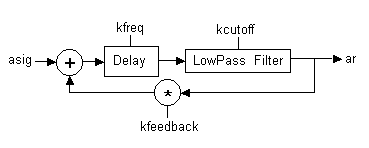
\includegraphics[scale=1]{wguide1} 


 wguide1.
\subsection*{Examples}


  Here is an example of the wguide1 opcode. It uses the files \emph{wguide1.orc}
 and \emph{wguide1.sco}
. 


 \textbf{Example 1. Example of the wguide1 opcode.}

\begin{lstlisting}
/* wguide1.orc */
; Initialize the global variables.
sr = 44100
kr = 4410
ksmps = 10
nchnls = 1

; Instrument #1 - a simple noise waveform.
instr 1
  ; Generate some noise.
  asig noise 20000, 0.5

  out asig
endin

; Instrument #2 - a waveguide example.
instr 2
  ; Generate some noise.
  asig noise 20000, 0.5

  ; Run it through a wave-guide model.
  kfreq init 200
  kcutoff init 3000
  kfeedback init 0.8
  awg1 wguide1 asig, kfreq, kcutoff, kfeedback

  out awg1
endin
/* wguide1.orc */
        
\end{lstlisting}
\begin{lstlisting}
/* wguide1.sco */
; Play Instrument #1 for 2 seconds.
i 1 0 2
; Play Instrument #2 for 2 seconds.
i 2 2 2
e
/* wguide1.sco */
        
\end{lstlisting}
\subsection*{See Also}


 \emph{wguide2}

\subsection*{Credits}


 


 


\begin{tabular}{ccc}
Author: Gabriel Maldonado &Italy &October 1998

\end{tabular}



 


 Example written by Kevin Conder.


 New in Csound version 3.49
%\hline 


\begin{comment}
\begin{tabular}{lcr}
Previous &Home &Next \\
wgpluck2 &Up &wguide2

\end{tabular}


\end{document}
\end{comment}

\newpage
\begin{comment}
\documentclass[10pt]{article}
\usepackage{fullpage, graphicx, url}
\setlength{\parskip}{1ex}
\setlength{\parindent}{0ex}
\title{wguide2}
\begin{document}


\begin{tabular}{ccc}
The Alternative Csound Reference Manual & & \\
Previous & &Next

\end{tabular}

%\hline 
\end{comment}
\section{wguide2}
wguide2�--� A model of beaten plate consisting of two parallel delay-lines and two first-order lowpass filters. \subsection*{Description}


  A model of beaten plate consisting of two parallel delay-lines and two first-order lowpass filters. 
\subsection*{Syntax}


 ar \textbf{wguide2}
 asig, xfreq1, xfreq2, kcutoff1, kcutoff2, kfeedback1, kfeedback2
\subsection*{Performance}


 \emph{asig}
 -- the input of excitation noise 


 \emph{xfreq1, xfreq2}
 -- the frequency (i.e. the inverse of delay time) Changed to x-rate in Csound version 3.59. 


 \emph{kcutoff1, kcutoff2}
 -- the filter cutoff frequency in Hz. 


 \emph{kfeedback1, kfeedback2}
 -- the feedback factor 


 \emph{wguide2}
 is a model of beaten plate consisting of two parallel delay-lines and two first-order lowpass filters. The two feedback lines are mixed and sent to the delay again each cycle. 


  Implementing waveguide algorithms as opcodes, instead of orc instruments, allows the user to set \emph{kr}
 different than \emph{sr}
, allowing better performance particulary when using real-time. 


 


 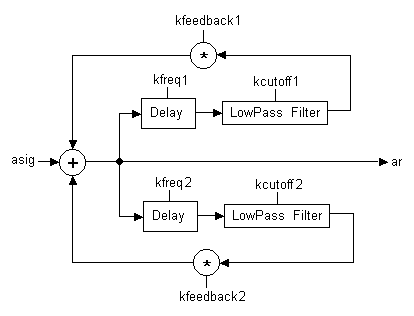
\includegraphics[scale=1]{wguide2} 


 wguide2.
\subsection*{See Also}


 \emph{wguide1}

\subsection*{Credits}


 


 


\begin{tabular}{ccc}
Author: Gabriel Maldonado &Italy &October 1998

\end{tabular}



 


 New in Csound version 3.49
%\hline 


\begin{comment}
\begin{tabular}{lcr}
Previous &Home &Next \\
wguide1 &Up &wrap

\end{tabular}


\end{document}
\end{comment}

\newpage
\begin{comment}
\documentclass[10pt]{article}
\usepackage{fullpage, graphicx, url}
\setlength{\parskip}{1ex}
\setlength{\parindent}{0ex}
\title{wrap}
\begin{document}


\begin{tabular}{ccc}
The Alternative Csound Reference Manual & & \\
Previous & &Next

\end{tabular}

%\hline 
\end{comment}
\section{wrap}
wrap�--� Wraps-around the signal that exceeds the low and high thresholds. \subsection*{Description}


  Wraps-around the signal that exceeds the low and high thresholds. 
\subsection*{Syntax}


 ar \textbf{wrap}
 asig, klow, khigh


 ir \textbf{wrap}
 isig, ilow, ihigh


 kr \textbf{wrap}
 ksig, klow, khigh
\subsection*{Initialization}


 \emph{isig}
 -- input signal 


 \emph{ilow}
 -- low threshold 


 \emph{ihigh}
 -- high threshold 
\subsection*{Performance}


 \emph{xsig}
 -- input signal 


 \emph{klow}
 -- low threshold 


 \emph{khigh}
 -- high threshold 


 \emph{wrap}
 wraps-around the signal that exceeds the low and high thresholds. 


  This opcode is useful in several situations, such as table indexing or for clipping and modeling a-rate, i-rate or k-rate signals. \emph{wrap}
 is also useful for wrap-around of table data when the maximum index is not a power of two (see \emph{table}
 and \emph{tablei}
). Another use of \emph{wrap}
 is in cyclical event repeating, with arbitrary cycle length. 
\subsection*{See Also}


 \emph{limit}
, \emph{mirror}

\subsection*{Credits}


 


 


\begin{tabular}{cc}
Author: Gabriel Maldonado &Italy

\end{tabular}



 


 New in Csound version 3.49
%\hline 


\begin{comment}
\begin{tabular}{lcr}
Previous &Home &Next \\
wguide2 &Up &wterrain

\end{tabular}


\end{document}
\end{comment}

\newpage
\begin{comment}
\documentclass[10pt]{article}
\usepackage{fullpage, graphicx, url}
\setlength{\parskip}{1ex}
\setlength{\parindent}{0ex}
\title{wterrain}
\begin{document}


\begin{tabular}{ccc}
The Alternative Csound Reference Manual & & \\
Previous & &Next

\end{tabular}

%\hline 
\end{comment}
\section{wterrain}
wterrain�--� A simple wave-terrain synthesis opcode. \subsection*{Description}


  A simple wave-terrain synthesis opcode. 
\subsection*{Syntax}


 aout \textbf{wterrain}
 kamp, kpch, k\_xcenter, k\_ycenter, k\_xradius, k\_yradius, itabx, itaby
\subsection*{Initialization}


 \emph{itabx, itaby}
 -- The two tables that define the terrain. 
\subsection*{Performance}


  The output is the result of drawing an ellipse with axes \emph{k\_xradius}
 and \emph{k\_yradius}
 centered at (\emph{k\_xcenter}
, \emph{k\_ycenter}
), and traversing it at frequency \emph{kpch}
. 
\subsection*{Examples}


  Here is an example of the wterrain opcode. It uses the files \emph{wterrain.orc}
 and \emph{wterrain.sco}
. 


 \textbf{Example 1. Example of the wterrain opcode.}

\begin{lstlisting}
/* wterrain.orc */
; Initialize the global variables.
sr = 44100
kr = 4410
ksmps = 10
nchnls = 1

instr 1
kdclk   linseg  0, 0.01, 1, p3-0.02, 1, 0.01, 0
kcx     line    0.1, p3, 1.9
krx     linseg  0.1, p3/2, 0.5, p3/2, 0.1
kpch    line    cpspch(p4), p3, p5 * cpspch(p4)
a1      wterrain    10000, kpch, kcx, kcx, -krx, krx, p6, p7
a1      dcblock a1
        out     a1*kdclk
endin
/* wterrain.orc */
        
\end{lstlisting}
\begin{lstlisting}
/* wterrain.sco */
f1      0       8192    10      1 0 0.33 0 0.2 0 0.14 0 0.11
f2      0       4096    10      1

i1      0       4       7.00 1 1 1
i1      4       4       6.07 1 1 2
i1      8       8       6.00 1 2 2
e
/* wterrain.sco */
        
\end{lstlisting}
\subsection*{Credits}


 


 


\begin{tabular}{cc}
Author: Matthew Gillard &New in version 4.19

\end{tabular}



 
%\hline 


\begin{comment}
\begin{tabular}{lcr}
Previous &Home &Next \\
wrap &Up &xadsr

\end{tabular}


\end{document}
\end{comment}

\newpage
%\begin{comment}
\documentclass[10pt]{article}
\usepackage{fullpage, graphicx, url}
\setlength{\parskip}{1ex}
\setlength{\parindent}{0ex}
\title{x Statement}
\begin{document}


\begin{tabular}{ccc}
The Alternative Csound Reference Manual & & \\
Previous & &Next

\end{tabular}

%\hline 
\end{comment}
\section{x Statement}
x�--� Skip the rest of the current section. \subsection*{Description}


  This statement may be used to skip the rest of the current section. 
\subsection*{Syntax}


 \textbf{x}
 anything
\subsection*{Initialization}


  All pfields are ignored. 
%\hline 


\begin{comment}
\begin{tabular}{lcr}
Previous &Home &Next \\
v Statement &Up &GEN Routines

\end{tabular}


\end{document}
\end{comment}

\begin{comment}
\documentclass[10pt]{article}
\usepackage{fullpage, graphicx, url}
\setlength{\parskip}{1ex}
\setlength{\parindent}{0ex}
\title{xadsr}
\begin{document}


\begin{tabular}{ccc}
The Alternative Csound Reference Manual & & \\
Previous & &Next

\end{tabular}

%\hline 
\end{comment}
\section{xadsr}
xadsr�--� Calculates the classical ADSR envelope. \subsection*{Description}


  Calculates the classical ADSR envelope 
\subsection*{Syntax}


 ar \textbf{xadsr}
 iatt, idec, islev, irel [, idel]


 kr \textbf{xadsr}
 iatt, idec, islev, irel [, idel]
\subsection*{Initialization}


 \emph{iatt}
 -- duration of attack phase 


 \emph{idec}
 -- duration of decay 


 \emph{islev}
 -- level for sustain phase 


 \emph{irel}
 -- duration of release phase 


 \emph{idel}
 -- period of zero before the envelope starts 
\subsection*{Performance}


  The envelope is the range 0 to 1 and may need to be scaled further. The envelope may be described as: 


 \includegraphics[scale=1]{adsr} 


 Picture of an ADSR envelope.


  The length of the sustain is calculated from the length of the note. This means \emph{adsr}
 is not suitable for use with MIDI events. The opcode \emph{xadsr}
 is identical to \emph{adsr}
 except it uses exponential, rather than linear, line segments. 


 \emph{xadsr}
 is new in Csound version 3.51. 
\subsection*{See Also}


 \emph{adsr}
, \emph{madsr}
, \emph{mxadsr}

%\hline 


\begin{comment}
\begin{tabular}{lcr}
Previous &Home &Next \\
wterrain &Up &xin

\end{tabular}


\end{document}
\end{comment}

\newpage
\begin{comment}
\documentclass[10pt]{article}
\usepackage{fullpage, graphicx, url}
\setlength{\parskip}{1ex}
\setlength{\parindent}{0ex}
\title{xin}
\begin{document}


\begin{tabular}{ccc}
The Alternative Csound Reference Manual & & \\
Previous & &Next

\end{tabular}

%\hline 
\end{comment}
\section{xin}
xin�--� Passes variables from a user-defined opcode block, \subsection*{Description}


  The \emph{xin}
 and \emph{xout}
 opcodes copy variables to and from the opcode definition, allowing communication with the calling instrument. 


  The types of input and output variables are defined by the parameters \emph{intypes}
 and \emph{outtypes}
. 


 


\begin{tabular}{cc}
\textbf{Notes}
 \\
� &

 


 
\begin{itemize}
\item 

 \emph{xin}
 and \emph{xout}
 should be called only once, and \emph{xin}
 should precede \emph{xout}
, otherwise an init error and deactivation of the current instrument may occur.

\item 

 These opcodes actually run only at i-time. Performance time copying is done by the user opcode call. This means that skipping \emph{xin}
 or \emph{xout}
 with \emph{kgoto}
 has no effect, while skipping with \emph{igoto}
 affects both init and performance time operation.


\end{itemize}


\end{tabular}

\subsection*{Syntax}


 xinarg1 [, xinarg2] ... [xinargN] \textbf{xin}

\subsection*{Performance}


 \emph{xinarg1}
, \emph{xinarg2}
, ... - input arguments. The number and type of variables must agree with the user-defined opcode's \emph{intypes}
 declaration. However, \emph{xin}
 does not check for incorrect use of init-time and control-rate variables. 


  The syntax of a user-defined opcode block is as follows: 


 opcode��name,�outtypes,�intypes\\ 
 xinarg1�[,�xinarg2]�[,�xinarg3]�...�[xinargN]��xin\\ 
 [setksmps��iksmps]\\ 
 ...�the�rest�of�the�instrument's�code.\\ 
 xout��xoutarg1�[,�xoutarg2]�[,�xoutarg3]�...�[xoutargN]\\ 
 endop\\ 
 ������


  The new opcode can then be used with the usual syntax: 


 [xinarg1]�[,�xinarg2]�...�[xinargN]��name��[xoutarg1]�[,�xoutarg2]�...�[xoutargN]�[,�iksmps]\\ 
 ������
\subsection*{Examples}


  See the example for the \emph{opcode}
 opcode. 
\subsection*{See Also}


 \emph{endop}
, \emph{opcode}
, \emph{setksmps}
, \emph{xout}

\subsection*{Credits}


 Author: Istvan Varga, 2002; based on code by Matt J. Ingalls


 New in version 4.22
%\hline 


\begin{comment}
\begin{tabular}{lcr}
Previous &Home &Next \\
xadsr &Up &xout

\end{tabular}


\end{document}
\end{comment}

\newpage
\begin{comment}
\documentclass[10pt]{article}
\usepackage{fullpage, graphicx, url}
\setlength{\parskip}{1ex}
\setlength{\parindent}{0ex}
\title{xout}
\begin{document}


\begin{tabular}{ccc}
The Alternative Csound Reference Manual & & \\
Previous & &Next

\end{tabular}

%\hline 
\end{comment}
\section{xout}
xout�--� Retrieves variables from a user-defined opcode block, \subsection*{Description}


  The \emph{xin}
 and \emph{xout}
 opcodes copy variables to and from the opcode definition, allowing communication with the calling instrument. 


  The types of input and output variables are defined by the parameters \emph{intypes}
 and \emph{outtypes}
. 


 


\begin{tabular}{cc}
\textbf{Notes}
 \\
� &

 


 
\begin{itemize}
\item 

 \emph{xin}
 and \emph{xout}
 should be called only once, and \emph{xin}
 should precede \emph{xout}
, otherwise an init error and deactivation of the current instrument may occur.

\item 

 These opcodes actually run only at i-time. Performance time copying is done by the user opcode call. This means that skipping \emph{xin}
 or \emph{xout}
 with \emph{kgoto}
 has no effect, while skipping with \emph{igoto}
 affects both init and performance time operation.


\end{itemize}


\end{tabular}

\subsection*{Syntax}


 \textbf{xout}
 xoutarg1 [, xoutarg2] ... [, xoutargN]
\subsection*{Performance}


 \emph{xoutarg1}
, \emph{xoutarg2}
, ... - output arguments. The number and type of variables must agree with the user-defined opcode's \emph{outtypes}
 declaration. However, \emph{xout}
 does not check for incorrect use of init-time and control-rate variables. 


  The syntax of a user-defined opcode block is as follows: 


 opcode��name,�outtypes,�intypes\\ 
 xinarg1�[,�xinarg2]�[,�xinarg3]�...�[xinargN]��xin\\ 
 [setksmps��iksmps]\\ 
 ...�the�rest�of�the�instrument's�code.\\ 
 xout��xoutarg1�[,�xoutarg2]�[,�xoutarg3]�...�[xoutargN]\\ 
 endop\\ 
 ������


  The new opcode can then be used with the usual syntax: 


 [xinarg1]�[,�xinarg2]�...�[xinargN]��name��[xoutarg1]�[,�xoutarg2]�...�[xoutargN]�[,�iksmps]\\ 
 ������
\subsection*{Examples}


  See the example for the \emph{opcode}
 opcode. 
\subsection*{See Also}


 \emph{endop}
, \emph{opcode}
, \emph{setksmps}
, \emph{xin}

\subsection*{Credits}


 Author: Istvan Varga, 2002; based on code by Matt J. Ingalls


 New in version 4.22
%\hline 


\begin{comment}
\begin{tabular}{lcr}
Previous &Home &Next \\
xin &Up &xscanmap

\end{tabular}


\end{document}
\end{comment}

\newpage
\begin{comment}
\documentclass[10pt]{article}
\usepackage{fullpage, graphicx, url}
\setlength{\parskip}{1ex}
\setlength{\parindent}{0ex}
\title{xscanmap}
\begin{document}


\begin{tabular}{ccc}
The Alternative Csound Reference Manual & & \\
Previous & &Next

\end{tabular}

%\hline 
\end{comment}
\section{xscanmap}
xscanmap�--� Allows the position and velocity of a node in a scanned process to be read. \subsection*{Description}


  Allows the position and velocity of a node in a scanned process to be read. 
\subsection*{Syntax}


 kpos, kvel \textbf{xscanmap}
 iscan, kamp, kvamp [, iwhich]
\subsection*{Initialization}


 \emph{iscan}
 -- which scan process to read 


 \emph{iwhich}
 (optional) -- which node to sense. The default is 0. 
\subsection*{Performance}


 \emph{kamp}
 -- amount to amplify the \emph{kpos}
 value. 


 \emph{kvamp}
 -- amount to amplify the \emph{kvel}
 value. 


  The internal state of a node is read. This includes its position and velocity. They are amplified by the \emph{kamp}
 and \emph{kvamp}
 values. 
\subsection*{Credits}


 Author: John ffitch


 New in version 4.20
%\hline 


\begin{comment}
\begin{tabular}{lcr}
Previous &Home &Next \\
xout &Up &xscansmap

\end{tabular}


\end{document}
\end{comment}

\newpage
\begin{comment}
\documentclass[10pt]{article}
\usepackage{fullpage, graphicx, url}
\setlength{\parskip}{1ex}
\setlength{\parindent}{0ex}
\title{xscans}
\begin{document}


\begin{tabular}{ccc}
The Alternative Csound Reference Manual & & \\
Previous & &Next

\end{tabular}

%\hline 
\end{comment}
\section{xscans}
xscans�--� Fast scanned synthesis waveform and the wavetable generator. \subsection*{Description}


  Experimental version of \emph{scans}
. Allows much larger matrices and is faster and smaller but removes some (unused?) flexibility. If liked, it will replace the older opcode as it is syntax compatible but extended. 
\subsection*{Syntax}


 ar \textbf{xscans}
 kamp, kfreq, ifntraj, id [, iorder]
\subsection*{Initialization}


 \emph{ifntraj}
 -- table containing the scanning trajectory. This is a series of numbers that contains addresses of masses. The order of these addresses is used as the scan path. It should not contain values greater than the number of masses, or negative numbers. See the \emph{introduction to the scanned synthesis section}
. 


 \emph{id}
 -- If positive, the ID of the opcode. This will be used to point the scanning opcode to the proper waveform maker. If this value is negative, the absolute of this value is the wavetable on which to write the waveshape. That wavetable can be used later from an other opcode to generate sound. The initial contents of this table will be destroyed. 


 \emph{iorder}
 (optional, default=0) -- order of interpolation used internally. It can take any value in the range 1 to 4, and defaults to 4, which is quartic interpolation. The setting of 2 is quadratic and 1 is linear. The higher numbers are slower, but not necessarily better. 
\subsection*{Performance}


 \emph{kamp}
 -- output amplitude. Note that the resulting amplitude is also dependent on instantaneous value in the wavetable. This number is effectively the scaling factor of the wavetable. 


 \emph{kfreq}
 -- frequency of the scan rate 
\subsection*{Matrix Format}


  The new matrix format is a list of connections, one per line linking point x to point y. There is no weight given to the link; it is assumed to be unity. The list is proceeded by the line $<$MATRIX$>$ and ends with a $<$/MATRIX$>$ line 


  For example, a circular string of 8 would be coded as 


 
\begin{lstlisting}
<MATRIX>
0 1
1 0
1 2
2 1
2 3
3 2
3 4
4 3
4 5
5 4
5 6
6 5
6 7
7 6
0 7
</MATRIX>
        
\end{lstlisting}


 
\subsection*{Examples}


  For an example, see the documentation on \emph{scans}
. 
\subsection*{See Also}


 \emph{scans}
, \emph{xscanu}

%\hline 


\begin{comment}
\begin{tabular}{lcr}
Previous &Home &Next \\
xscansmap &Up &xscanu

\end{tabular}


\end{document}
\end{comment}

\newpage
\begin{comment}
\documentclass[10pt]{article}
\usepackage{fullpage, graphicx, url}
\setlength{\parskip}{1ex}
\setlength{\parindent}{0ex}
\title{xscansmap}
\begin{document}


\begin{tabular}{ccc}
The Alternative Csound Reference Manual & & \\
Previous & &Next

\end{tabular}

%\hline 
\end{comment}
\section{xscansmap}
xscansmap�--� Allows the position and velocity of a node in a scanned process to be read. \subsection*{Description}


  Allows the position and velocity of a node in a scanned process to be read. 
\subsection*{Syntax}


 \textbf{xscansmap}
 kpos, kvel, iscan, kamp, kvamp [, iwhich]
\subsection*{Initialization}


 \emph{iscan}
 -- which scan process to read 


 \emph{iwhich}
 (optional) -- which node to sense. The default is 0. 
\subsection*{Performance}


 \emph{kpos}
 -- the node's postion. 


 \emph{kvel}
 -- the node's velocity. 


 \emph{kamp}
 -- amount to amplify the \emph{kpos}
 value. 


 \emph{kvamp}
 -- amount to amplify the \emph{kvel}
 value. 


  The internal state of a node is read. This includes its position and velocity. They are amplified by the \emph{kamp}
 and \emph{kvamp}
 values. 
\subsection*{Credits}


 New in version 4.21


 November 2002. Thanks to Rasmus Ekman for pointing this opcode out.
%\hline 


\begin{comment}
\begin{tabular}{lcr}
Previous &Home &Next \\
xscanmap &Up &xscans

\end{tabular}


\end{document}
\end{comment}

\newpage
\begin{comment}
\documentclass[10pt]{article}
\usepackage{fullpage, graphicx, url}
\setlength{\parskip}{1ex}
\setlength{\parindent}{0ex}
\title{xscanu}
\begin{document}


\begin{tabular}{ccc}
The Alternative Csound Reference Manual & & \\
Previous & &Next

\end{tabular}

%\hline 
\end{comment}
\section{xscanu}
xscanu�--� Compute the waveform and the wavetable for use in scanned synthesis. \subsection*{Description}


  Experimental version of \emph{scanu}
. Allows much larger matrices and is faster and smaller but removes some (unused?) flexibility. If liked, it will replace the older opcode as it is syntax compatible but extended. 
\subsection*{Syntax}


 \textbf{xscanu}
 init, irate, ifnvel, ifnmass, ifnstif, ifncentr, ifndamp, kmass, kstif, kcentr, kdamp, ileft, iright, kpos, kstrngth, ain, idisp, id
\subsection*{Initialization}


 \emph{init}
 -- the initial position of the masses. If this is a negative number, then the absolute of init signifies the table to use as a hammer shape. If init $>$ 0, the length of it should be the same as the intended mass number, otherwise it can be anything. 


 \emph{irate}
 -- update rate. 


 \emph{ifnvel}
 -- the ftable that contains the initial velocity for each mass. It should have the same size as the intended mass number. 


 \emph{ifnmass}
 -- ftable that contains the mass of each mass. It should have the same size as the intended mass number. 


 \emph{ifnstif}
 -- 


 
\begin{itemize}
\item 

 \emph{either}
 an ftable that contains the spring stiffness of each connection. It should have the same size as the square of the intended mass number. The data ordering is a row after row dump of the connection matrix of the system.

\item 

 \emph{or}
 a string giving the name of a file in the MATRIX format


\end{itemize}


 \emph{ifncentr}
 -- ftable that contains the centering force of each mass. It should have the same size as the intended mass number. 


 \emph{ifndamp}
 -- the ftable that contains the damping factor of each mass. It should have the same size as the intended mass number. 


 \emph{ileft}
 -- If init $<$ 0, the position of the left hammer (ileft = 0 is hit at leftmost, ileft = 1 is hit at rightmost). 


 \emph{iright}
 -- If init $<$ 0, the position of the right hammer (iright = 0 is hit at leftmost, iright = 1 is hit at rightmost). 


 \emph{idisp}
 -- If 0, no display of the masses is provided. 


 \emph{id}
 -- If positive, the ID of the opcode. This will be used to point the scanning opcode to the proper waveform maker. If this value is negative, the absolute of this value is the wavetable on which to write the waveshape. That wavetable can be used later from an other opcode to generate sound. The initial contents of this table will be destroyed. 
\subsection*{Performance}


 \emph{kmass}
 -- scales the masses 


 \emph{kstif}
 -- scales the spring stiffness 


 \emph{kcentr}
 -- scales the centering force 


 \emph{kdamp}
 -- scales the damping 


 \emph{kpos}
 -- position of an active hammer along the string (kpos = 0 is leftmost, kpos = 1 is rightmost). The shape of the hammer is determined by init and the power it pushes with is kstrngth. 


 \emph{kstrngth}
 -- power that the active hammer uses 


 \emph{ain}
 -- audio input that adds to the velocity of the masses. Amplitude should not be too great. 
\subsection*{Matrix Format}


  The new matrix format is a list of connections, one per line linking point x to point y. There is no weight given to the link; it is assumed to be unity. The list is proceeded by the line $<$MATRIX$>$ and ends with a $<$/MATRIX$>$ line 


  For example, a circular string of 8 would be coded as 


 
\begin{lstlisting}
<MATRIX>
0 1
1 0
1 2
2 1
2 3
3 2
3 4
4 3
4 5
5 4
5 6
6 5
6 7
7 6
0 7
</MATRIX>
        
\end{lstlisting}


 
\subsection*{Examples}


  For an example, see the documentation on \emph{scans}
. 
\subsection*{See Also}


 \emph{scanu}
, \emph{xscans}

%\hline 


\begin{comment}
\begin{tabular}{lcr}
Previous &Home &Next \\
xscans &Up &xtratim

\end{tabular}


\end{document}
\end{comment}

\newpage
\begin{comment}
\documentclass[10pt]{article}
\usepackage{fullpage, graphicx, url}
\setlength{\parskip}{1ex}
\setlength{\parindent}{0ex}
\title{xtratim}
\begin{document}


\begin{tabular}{ccc}
The Alternative Csound Reference Manual & & \\
Previous & &Next

\end{tabular}

%\hline 
\end{comment}
\section{xtratim}
xtratim�--� Extend the duration of real-time generated events. \subsection*{Description}


  Extend the duration of real-time generated events and handle their extra life (see also \emph{linenr}
). 
\subsection*{Syntax}


 \textbf{xtratim}
 iextradur
\subsection*{Initialization}


 \emph{iextradur}
 -- additional duration of current instrument instance 
\subsection*{Performance}


 \emph{xtratim}
 extends current MIDI-activated note duration of \emph{iextradur}
 seconds after the corresponding noteoff message has deactivated current note itself. This opcode has no output arguments. 


  This opcode is useful for implementing complex release-oriented envelopes. 
\subsection*{Examples}


 


 
\begin{lstlisting}
 \emph{instr}
 1 ;allows complex ADSR envelope with MIDI events
  inum \emph{notnum}

  icps \emph{cpsmidi}

  iamp \emph{ampmid}
i 4000
 ;
 ;------- complex envelope block ------
  \emph{xtratim}
 1 ;extra-time, i.e. release dur
  krel \emph{init}
 0
  krel \emph{release}
 ;outputs release-stage flag (0 or 1 values)
  if (krel  .5) \emph{kgoto}
 rel ;if in release-stage goto release section
 ;
 ;************ attack and sustain section ***********
  kmp1 \emph{linseg}
 0, .03, 1, .05, 1, .07, 0, .08, .5, 4, 1, 50, 1
  kmp = kmp1*iamp
   \emph{kgoto}
 done
 ;
 ;--------- release section --------
   rel:
  kmp2 \emph{linseg}
 1, .3, .2, .7, 0
  kmp = kmp1*kmp2*iamp
  done:
 ;------
  a1 \emph{oscili}
 kmp, icps, 1
  \emph{out}
 a1
 \emph{endin}

        
\end{lstlisting}


 
\subsection*{See Also}


 \emph{linenr}
, \emph{release}

\subsection*{Credits}


 


 


\begin{tabular}{cc}
Author: Gabriel Maldonado &Italy

\end{tabular}



 


 New in Csound version 3.47
%\hline 


\begin{comment}
\begin{tabular}{lcr}
Previous &Home &Next \\
xscanu &Up &xyin

\end{tabular}


\end{document}
\end{comment}

\newpage
\begin{comment}
\documentclass[10pt]{article}
\usepackage{fullpage, graphicx, url}
\setlength{\parskip}{1ex}
\setlength{\parindent}{0ex}
\title{xyin}
\begin{document}


\begin{tabular}{ccc}
The Alternative Csound Reference Manual & & \\
Previous & &Next

\end{tabular}

%\hline 
\end{comment}
\section{xyin}
xyin�--� Sense the cursor position in an output window \subsection*{Description}


  Sense the cursor position in an output window. When \emph{xyin}
 is called the position of the mouse within the output window is used to reply to the request. This simple mechanism does mean that only one \emph{xyin}
 can be used accurately at once. The position of the mouse is reported in the output window. 
\subsection*{Syntax}


 kx, ky \textbf{xyin}
 iprd, ixmin, ixmax, iymin, iymax [, ixinit] [, iyinit]
\subsection*{Initialization}


 \emph{iprd}
 -- period of cursor sensing (in seconds). Typically .1 seconds. 


 \emph{xmin, xmax, ymin, ymax}
 -- edge values for the x-y coordinates of a cursor in the input window. 


 \emph{ixinit, iyinit}
 (optional) -- initial x-y coordinates reported; the default values are 0,0. If these values are not within the given min-max range, they will be coerced into that range. 
\subsection*{Performance}


 \emph{xyin}
 samples the cursor x-y position in an input window every \emph{iprd}
 seconds. Output values are repeated (not interpolated) at the k-rate, and remain fixed until a new change is registered in the window. There may be any number of input windows. This unit is useful for real-time control, but continuous motion should be avoided if \emph{iprd}
 is unusually small. 
\subsection*{Examples}


  Here is an example of the xyin opcode. It uses the files \emph{xyin.orc}
 and \emph{xyin.sco}
. 


 \textbf{Example 1. Example of the xyin opcode.}

\begin{lstlisting}
/* xyin.orc */
; Initialize the global variables.
sr = 44100
kr = 4410
ksmps = 10
nchnls = 1

; Instrument #1.
instr 1
  ; Print and capture values every 0.1 seconds.
  iprd = 0.1
  ; The x values are from 1 to 30.
  ixmin = 1
  ixmax = 30
  ; The y values are from 1 to 30.
  iymin = 1
  iymax = 30
  ; The initial values for X and Y are both 15.
  ixinit = 15
  iyinit = 15

  ; Get the values kx and ky using the xyin opcode.
  kx, ky xyin iprd, ixmin, ixmax, iymin, iymax, ixinit, iyinit

  ; Print out the values of kx and ky.
  printks "kx=%f, ky=%f\\n", iprd, kx, ky

  ; Play an oscillator, use the x values for amplitude and
  ; the y values for frequency.
  kamp = kx * 1000
  kcps = ky * 220
  a1 oscil kamp, kcps, 1

  out a1
endin
/* xyin.orc */
        
\end{lstlisting}
\begin{lstlisting}
/* xyin.sco */
; Table #1, a sine wave.
f 1 0 16384 10 1

; Play Instrument #1 for 30 seconds.
i 1 0 30
e
/* xyin.sco */
        
\end{lstlisting}
 As the values of kx and ky change, they will be printed out like this: \begin{lstlisting}
kx=8.612036, ky=22.677933
kx=10.765685, ky=15.644135
      
\end{lstlisting}
\subsection*{Credits}


 Example written by Kevin Conder.
%\hline 


\begin{comment}
\begin{tabular}{lcr}
Previous &Home &Next \\
xtratim &Up &zacl

\end{tabular}


\end{document}
\end{comment}

\newpage
\begin{comment}
\documentclass[10pt]{article}
\usepackage{fullpage, graphicx, url}
\setlength{\parskip}{1ex}
\setlength{\parindent}{0ex}
\title{zacl}
\begin{document}


\begin{tabular}{ccc}
The Alternative Csound Reference Manual & & \\
Previous & &Next

\end{tabular}

%\hline 
\end{comment}
\section{zacl}
zacl�--� Clears one or more variables in the za space. \subsection*{Description}


  Clears one or more variables in the za space. 
\subsection*{Syntax}


 \textbf{zacl}
 kfirst, klast
\subsection*{Performance}


 \emph{kfirst}
 -- first zk or za location in the range to clear. 


 \emph{klast}
 -- last zk or za location in the range to clear. 


 \emph{zacl}
 clears one or more variables in the za space. This is useful for those variables which are used as accumulators for mixing a-rate signals at each cycle, but which must be cleared before the next set of calculations. 
\subsection*{Examples}


  Here is an example of the zacl opcode. It uses the files \emph{zacl.orc}
 and \emph{zacl.sco}
. 


 \textbf{Example 1. Example of the zacl opcode.}

\begin{lstlisting}
/* zacl.orc */
; Initialize the global variables.
sr = 44100
kr = 4410
ksmps = 10
nchnls = 1

; Initialize the ZAK space.
; Create 1 a-rate variable and 1 k-rate variable.
zakinit 1, 1

; Instrument #1 -- a simple waveform.
instr 1
  ; Generate a simple sine waveform.
  asin oscil 20000, 440, 1

  ; Send the sine waveform to za variable #1.
  zaw asin, 1
endin

; Instrument #2 -- generates audio output.
instr 2
  ; Read za variable #1.
  a1 zar 1

  ; Generate the audio output.
  out a1

  ; Clear the za variables, get them ready for 
  ; another pass.
  zacl 0, 1
endin
/* zacl.orc */
        
\end{lstlisting}
\begin{lstlisting}
/* zacl.sco */
; Table #1, a sine wave.
f 1 0 16384 10 1

; Play Instrument #1 for one second.
i 1 0 1
; Play Instrument #2 for one second.
i 2 0 1
e
/* zacl.sco */
        
\end{lstlisting}
\subsection*{See Also}


 \emph{zamod}
, \emph{zar}
, \emph{zaw}
, \emph{zawm}
, \emph{ziw}
, \emph{ziwm}

\subsection*{Credits}


 


 


\begin{tabular}{ccc}
Author: Robin Whittle &Australia &May 1997

\end{tabular}



 


 Example written by Kevin Conder.
%\hline 


\begin{comment}
\begin{tabular}{lcr}
Previous &Home &Next \\
xyin &Up &zakinit

\end{tabular}


\end{document}
\end{comment}

\newpage
\begin{comment}
\documentclass[10pt]{article}
\usepackage{fullpage, graphicx, url}
\setlength{\parskip}{1ex}
\setlength{\parindent}{0ex}
\title{zakinit}
\begin{document}


\begin{tabular}{ccc}
The Alternative Csound Reference Manual & & \\
Previous & &Next

\end{tabular}

%\hline 
\end{comment}
\section{zakinit}
zakinit�--� Establishes zak space. \subsection*{Description}


  Establishes zak space. Must be called only once. 
\subsection*{Syntax}


 \textbf{zakinit}
 isizea, isizek
\subsection*{Initialization}


 \emph{isizea}
 -- the number of audio rate locations for a-rate patching. Each location is actually an array which is ksmps long. 


 \emph{isizek}
 -- the number of locations to reserve for floats in the zk space. These can be written and read at i- and k-rates. 
\subsection*{Performance}


  At least one location each is always allocated for both za and zk spaces. There can be thousands or tens of thousands za and zk ranges, but most pieces probably only need a few dozen for patching signals. These patching locations are referred to by number in the other zak opcodes. 


  To run \emph{zakinit}
 only once, put it outside any instrument definition, in the orchestra file header, after \emph{sr}
, \emph{kr}
, \emph{ksmps}
, and \emph{nchnls}
. 
\subsection*{Examples}


  Here is an example of the zakinit opcode. It uses the files \emph{zakinit.orc}
 and \emph{zakinit.sco}
. 


 \textbf{Example 1. Example of the zakinit opcode.}

\begin{lstlisting}
/* zakinit.orc */
; Initialize the global variables.
sr = 44100
kr = 4410
ksmps = 10
nchnls = 1

; Initialize the ZAK space.
; Create 3 a-rate variables and 5 k-rate variables.
zakinit 3, 5

; Instrument #1 -- a simple waveform.
instr 1
  ; Generate a simple sine waveform.
  asin oscil 20000, 440, 1

  ; Send the sine waveform to za variable #1.
  zaw asin, 1
endin

; Instrument #2 -- generates audio output.
instr 2
  ; Read za variable #1.
  a1 zar 1

  ; Generate audio output.
  out a1

  ; Clear the za variables, get them ready for 
  ; another pass.
  zacl 0, 3
endin
/* zakinit.orc */
        
\end{lstlisting}
\begin{lstlisting}
/* zakinit.sco */
; Table #1, a sine wave.
f 1 0 16384 10 1

; Play Instrument #1 for one second.
i 1 0 1
; Play Instrument #2 for one second.
i 2 0 1
e
/* zakinit.sco */
        
\end{lstlisting}
\subsection*{Credits}


 


 


\begin{tabular}{ccc}
Author: Robin Whittle &Australia &May 1997

\end{tabular}



 


 Example written by Kevin Conder.
%\hline 


\begin{comment}
\begin{tabular}{lcr}
Previous &Home &Next \\
zacl &Up &zamod

\end{tabular}


\end{document}
\end{comment}

\newpage
%\begin{comment}
\documentclass[10pt]{article}
\usepackage{fullpage, graphicx, url}
\setlength{\parskip}{1ex}
\setlength{\parindent}{0ex}
\title{Zak Patch System}
\begin{document}


\begin{tabular}{ccc}
The Alternative Csound Reference Manual & & \\
Previous & &Next

\end{tabular}

%\hline 
\end{comment}
\section{Zak Patch System}


  The zak opcodes are used to create a system for i-rate, k-rate or a-rate patching. The zak system can be thought of as a global array of variables. These opcodes are useful for performing flexible patching or routing from one instrument to another. The system is similar to a patching matrix on a mixing console or to a modulation matrix on a synthesizer. It is also useful whenever an array of variables is required. 


  The zak system is initialized by the \emph{zakinit}
 opcode, which is usually placed just after the other global initializations: \emph{sr}
, \emph{kr}
, \emph{ksmps}
, \emph{nchnls}
. The \emph{zakinit}
 opcode defines two areas of memory, one area for i- and k-rate patching, and the other area for a-rate patching. The \emph{zakinit}
 opcode may only be called once. Once the zak space is initialized, other zak opcodes can be used to read from, and write to the zak memory space, as well as perform various other tasks. 


  Opcodes for the zak patch system are \emph{zacl}
, \emph{zakinit}
, \emph{zamod}
, \emph{zar}
, \emph{zarg}
, \emph{zaw}
, \emph{zawm}
, \emph{zir}
, \emph{ziw}
, \emph{ziwm}
, \emph{zkcl}
, \emph{zkmod}
, \emph{zkr}
, \emph{zkw}
, and \emph{zkwm}
. 
%\hline 


\begin{comment}
\begin{tabular}{lcr}
Previous &Home &Next \\
Tools for Real-time Spectral Processing &Up &The Standard Numeric Score

\end{tabular}


\end{document}
\end{comment}

\begin{comment}
\documentclass[10pt]{article}
\usepackage{fullpage, graphicx, url}
\setlength{\parskip}{1ex}
\setlength{\parindent}{0ex}
\title{zamod}
\begin{document}


\begin{tabular}{ccc}
The Alternative Csound Reference Manual & & \\
Previous & &Next

\end{tabular}

%\hline 
\end{comment}
\section{zamod}
zamod�--� Modulates one a-rate signal by a second one. \subsection*{Description}


  Modulates one a-rate signal by a second one. 
\subsection*{Syntax}


 ar \textbf{zamod}
 asig, kzamod
\subsection*{Performance}


 \emph{asig}
 -- the input signal 


 \emph{kzamod}
 -- controls which za variable is used for modulation. A positive value means additive modulation, a negative value means multiplicative modulation. A value of 0 means no change to \emph{asig}
. 


 \emph{zamod}
 modulates one a-rate signal by a second one, which comes from a za variable. The location of the modulating variable is controlled by the i-rate or k-rate variable \emph{kzamod}
. This is the a-rate version of \emph{zkmod}
. 
\subsection*{Examples}


  Here is an example of the zamod opcode. It uses the files \emph{zamod.orc}
 and \emph{zamod.sco}
. 


 \textbf{Example 1. Example of the zamod opcode.}

\begin{lstlisting}
/* zamod.orc */
; Initialize the global variables.
sr = 44100
kr = 4410
ksmps = 10
nchnls = 1

; Initialize the ZAK space.
; Create 2 a-rate variables and 2 k-rate variables.
zakinit 2, 2

; Instrument #1 -- a simple waveform.
instr 1
  ; Vary an a-rate signal linearly from 20,000 to 0.
  asig line 20000, p3, 0

  ; Send the signal to za variable #1.
  zaw asig, 1
endin

; Instrument #2 -- generates audio output.
instr 2
  ; Generate a simple sine wave.
  asin oscil 1, 440, 1
  
  ; Modify the sine wave, multiply its amplitude by 
  ; za variable #1.
  a1 zamod asin, -1

  ; Generate the audio output.
  out a1

  ; Clear the za variables, prepare them for 
  ; another pass.
  zacl 0, 2
endin
/* zamod.orc */
        
\end{lstlisting}
\begin{lstlisting}
/* zamod.sco */
; Table #1, a sine wave.
f 1 0 16384 10 1

; Play Instrument #1 for 2 seconds.
i 1 0 2
; Play Instrument #2 for 2 seconds.
i 2 0 2
e
/* zamod.sco */
        
\end{lstlisting}
\subsection*{See Also}


 \emph{zacl}
, \emph{ziw}
, \emph{ziwm}

\subsection*{Credits}


 


 


\begin{tabular}{ccc}
Author: Robin Whittle &Australia &May 1997

\end{tabular}



 


 Example written by Kevin Conder.
%\hline 


\begin{comment}
\begin{tabular}{lcr}
Previous &Home &Next \\
zakinit &Up &zar

\end{tabular}


\end{document}
\end{comment}

\newpage
\begin{comment}
\documentclass[10pt]{article}
\usepackage{fullpage, graphicx, url}
\setlength{\parskip}{1ex}
\setlength{\parindent}{0ex}
\title{zar}
\begin{document}


\begin{tabular}{ccc}
The Alternative Csound Reference Manual & & \\
Previous & &Next

\end{tabular}

%\hline 
\end{comment}
\section{zar}
zir�--� Reads from a location in za space at a-rate. \subsection*{Description}


  Reads from a location in za space at a-rate. 
\subsection*{Syntax}


 ar \textbf{zar}
 kndx
\subsection*{Performance}


 \emph{kndx}
 -- points to the za location to be read. 


 \emph{zar}
 reads the array of floats at \emph{kndx}
 in za space, which are ksmps number of a-rate floats to be processed in a k cycle. 
\subsection*{Examples}


  Here is an example of the zar opcode. It uses the files \emph{zar.orc}
 and \emph{zar.sco}
. 


 \textbf{Example 1. Example of the zar opcode.}

\begin{lstlisting}
/* zar.orc */
; Initialize the global variables.
sr = 44100
kr = 4410
ksmps = 10
nchnls = 1

; Initialize the ZAK space.
; Create 1 a-rate variable and 1 k-rate variable.
zakinit 1, 1

; Instrument #1 -- a simple waveform.
instr 1
  ; Generate a simple sine waveform.
  asin oscil 20000, 440, 1

  ; Send the sine waveform to za variable #1.
  zaw asin, 1
endin

; Instrument #2 -- generates audio output.
instr 2
  ; Read za variable #1.
  a1 zar 1

  ; Generate audio output.
  out a1

  ; Clear the za variables, get them ready for 
  ; another pass.
  zacl 0, 1
endin
/* zar.orc */
        
\end{lstlisting}
\begin{lstlisting}
/* zar.sco */
; Table #1, a sine wave.
f 1 0 16384 10 1

; Play Instrument #1 for one second.
i 1 0 1
; Play Instrument #2 for one second.
i 2 0 1
e
/* zar.sco */
        
\end{lstlisting}
\subsection*{See Also}


 \emph{zarg}
, \emph{zir}
, \emph{zkr}

\subsection*{Credits}


 


 


\begin{tabular}{ccc}
Author: Robin Whittle &Australia &May 1997

\end{tabular}



 


 Example written by Kevin Conder.
%\hline 


\begin{comment}
\begin{tabular}{lcr}
Previous &Home &Next \\
zamod &Up &zarg

\end{tabular}


\end{document}
\end{comment}

\newpage
\begin{comment}
\documentclass[10pt]{article}
\usepackage{fullpage, graphicx, url}
\setlength{\parskip}{1ex}
\setlength{\parindent}{0ex}
\title{zarg}
\begin{document}


\begin{tabular}{ccc}
The Alternative Csound Reference Manual & & \\
Previous & &Next

\end{tabular}

%\hline 
\end{comment}
\section{zarg}
zarg�--� Reads from a location in za space at a-rate, adds some gain. \subsection*{Description}


  Reads from a location in za space at a-rate, adds some gain. 
\subsection*{Syntax}


 ar \textbf{zarg}
 kndx, kgain
\subsection*{Initialization}


 \emph{kndx}
 -- points to the za location to be read. 


 \emph{kgain}
 -- multiplier for the a-rate signal. 
\subsection*{Performance}


 \emph{zarg}
 reads the array of floats at \emph{kndx}
 in za space, which are ksmps number of a-rate floats to be processed in a k cycle. \emph{zarg}
 also multiplies the a-rate signal by a k-rate value \emph{kgain}
. 
\subsection*{Examples}


  Here is an example of the zarg opcode. It uses the files \emph{zarg.orc}
 and \emph{zarg.sco}
. 


 \textbf{Example 1. Example of the zarg opcode.}

\begin{lstlisting}
/* zarg.orc */
; Initialize the global variables.
sr = 44100
kr = 4410
ksmps = 10
nchnls = 1

; Initialize the ZAK space.
; Create 1 a-rate variable and 1 k-rate variable.
zakinit 1, 1

; Instrument #1 -- a simple waveform.
instr 1
  ; Generate a simple sine waveform, with an amplitude 
  ; between 0 and 1.
  asin oscil 1, 440, 1

  ; Send the sine waveform to za variable #1.
  zaw asin, 1
endin

; Instrument #2 -- generates audio output.
instr 2
  ; Read za variable #1, multiply its amplitude by 20,000.
  a1 zarg 1, 20000

  ; Generate audio output.
  out a1

  ; Clear the za variables, get them ready for 
  ; another pass.
  zacl 0, 1
endin
/* zarg.orc */
        
\end{lstlisting}
\begin{lstlisting}
/* zarg.sco */
; Table #1, a sine wave.
f 1 0 16384 10 1

; Play Instrument #1 for one second.
i 1 0 1
; Play Instrument #2 for one second.
i 2 0 1
e
/* zarg.sco */
        
\end{lstlisting}
\subsection*{See Also}


 \emph{zar}
, \emph{zir}
, \emph{zkr}

\subsection*{Credits}


 


 


\begin{tabular}{ccc}
Author: Robin Whittle &Australia &May 1997

\end{tabular}



 


 Example written by Kevin Conder.
%\hline 


\begin{comment}
\begin{tabular}{lcr}
Previous &Home &Next \\
zar &Up &zaw

\end{tabular}


\end{document}
\end{comment}

\newpage
\begin{comment}
\documentclass[10pt]{article}
\usepackage{fullpage, graphicx, url}
\setlength{\parskip}{1ex}
\setlength{\parindent}{0ex}
\title{zaw}
\begin{document}


\begin{tabular}{ccc}
The Alternative Csound Reference Manual & & \\
Previous & &Next

\end{tabular}

%\hline 
\end{comment}
\section{zaw}
zaw�--� Writes to a za variable at a-rate without mixing. \subsection*{Description}


  Writes to a za variable at a-rate without mixing. 
\subsection*{Syntax}


 \textbf{zaw}
 asig, kndx
\subsection*{Performance}


 \emph{asig}
 -- value to be written to the za location. 


 \emph{kndx}
 -- points to the zk or za location to which to write. 


 \emph{zaw}
 writes \emph{asig}
 into the za variable specified by \emph{kndx}
. 


  These opcodes are fast, and always check that the index is within the range of zk or za space. If not, an error is reported, 0 is returned, and no writing takes place. 
\subsection*{Examples}


  Here is an example of the zaw opcode. It uses the files \emph{zaw.orc}
 and \emph{zaw.sco}
. 


 \textbf{Example 1. Example of the zaw opcode.}

\begin{lstlisting}
/* zaw.orc */
; Initialize the global variables.
sr = 44100
kr = 4410
ksmps = 10
nchnls = 1

; Initialize the ZAK space.
; Create 1 a-rate variable and 1 k-rate variable.
zakinit 1, 1

; Instrument #1 -- a simple waveform.
instr 1
  ; Generate a simple sine waveform.
  asin oscil 20000, 440, 1

  ; Send the sine waveform to za variable #1.
  zaw asin, 1
endin

; Instrument #2 -- generates audio output.
instr 2
  ; Read za variable #1.
  a1 zar 1

  ; Generate the audio output.
  out a1

  ; Clear the za variables, get them ready for 
  ; another pass.
  zacl 0, 1
endin
/* zaw.orc */
        
\end{lstlisting}
\begin{lstlisting}
/* zaw.sco */
; Table #1, a sine wave.
f 1 0 16384 10 1

; Play Instrument #1 for one second.
i 1 0 1
; Play Instrument #2 for one second.
i 2 0 1
e
/* zaw.sco */
        
\end{lstlisting}
\subsection*{See Also}


 \emph{zawm}
, \emph{ziw}
, \emph{ziwm}
, \emph{zkw}
, \emph{zkwm}

\subsection*{Credits}


 


 


\begin{tabular}{ccc}
Author: Robin Whittle &Australia &May 1997

\end{tabular}



 


 Example written by Kevin Conder.
%\hline 


\begin{comment}
\begin{tabular}{lcr}
Previous &Home &Next \\
zarg &Up &zawm

\end{tabular}


\end{document}
\end{comment}

\newpage
\begin{comment}
\documentclass[10pt]{article}
\usepackage{fullpage, graphicx, url}
\setlength{\parskip}{1ex}
\setlength{\parindent}{0ex}
\title{zawm}
\begin{document}


\begin{tabular}{ccc}
The Alternative Csound Reference Manual & & \\
Previous & &Next

\end{tabular}

%\hline 
\end{comment}
\section{zawm}
zawm�--� Writes to a za variable at a-rate with mixing. \subsection*{Description}


  Writes to a za variable at a-rate with mixing. 
\subsection*{Syntax}


 \textbf{zawm}
 asig, kndx [, imix]
\subsection*{Initialization}


 \emph{imix}
 (optional, default=1) -- indicates if mixing should occur. 
\subsection*{Performance}


 \emph{asig}
 -- value to be written to the za location. 


 \emph{kndx}
 -- points to the zk or za location to which to write. 


  These opcodes are fast, and always check that the index is within the range of zk or za space. If not, an error is reported, 0 is returned, and no writing takes place. 


 \emph{zawm}
 is a mixing opcode, it adds the signal to the current value of the variable. If no \emph{imix}
 is specified, mixing always occurs. \emph{imix}
 = 0 will cause overwriting like \emph{ziw}
, \emph{zkw}
, and \emph{zaw}
. Any other value will cause mixing. 


 \emph{Caution}
: When using the mixing opcodes \emph{ziwm}
, \emph{zkwm}
, and \emph{zawm}
, care must be taken that the variables mixed to, are zeroed at the end (or start) of each k- or a-cycle. Continuing to add signals to them, can cause their values can drift to astronomical figures. 


  One approach would be to establish certain ranges of zk or za variables to be used for mixing, then use \emph{zkcl}
 or \emph{zacl}
 to clear those ranges. 
\subsection*{Examples}


  Here is an example of the zawm opcode. It uses the files \emph{zawm.orc}
 and \emph{zawm.sco}
. 


 \textbf{Example 1. Example of the zawm opcode.}

\begin{lstlisting}
/* zawm.orc */
; Initialize the global variables.
sr = 44100
kr = 4410
ksmps = 10
nchnls = 1

; Initialize the ZAK space.
; Create 1 a-rate variable and 1 k-rate variable.
zakinit 1, 1

; Instrument #1 -- a basic instrument.
instr 1
  ; Generate a simple sine waveform.
  asin oscil 15000, 440, 1

  ; Mix the sine waveform with za variable #1.
  zawm asin, 1
endin

; Instrument #2 -- another basic instrument.
instr 2
  ; Generate another waveform with a different frequency.
  asin oscil 15000, 880, 1

  ; Mix this sine waveform with za variable #1.
  zawm asin, 1
endin

; Instrument #3 -- generates audio output.
instr 3
  ; Read za variable #1, containing both waveforms.
  a1 zar 1

  ; Generate the audio output.
  out a1

  ; Clear the za variables, get them ready for 
  ; another pass.
  zacl 0, 1
endin
/* zawm.orc */
        
\end{lstlisting}
\begin{lstlisting}
/* zawm.sco */
; Table #1, a sine wave.
f 1 0 16384 10 1

; Play Instrument #1 for one second.
i 1 0 1
; Play Instrument #2 for one second.
i 2 0 1
; Play Instrument #3 for one second.
i 3 0 1
e
/* zawm.sco */
        
\end{lstlisting}
\subsection*{See Also}


 \emph{zaw}
, \emph{ziw}
, \emph{ziwm}
, \emph{zkw}
, \emph{zkwm}

\subsection*{Credits}


 


 


\begin{tabular}{ccc}
Author: Robin Whittle &Australia &May 1997

\end{tabular}



 


 Example written by Kevin Conder.
%\hline 


\begin{comment}
\begin{tabular}{lcr}
Previous &Home &Next \\
zaw &Up &zfilter2

\end{tabular}


\end{document}
\end{comment}

\newpage
\begin{comment}
\documentclass[10pt]{article}
\usepackage{fullpage, graphicx, url}
\setlength{\parskip}{1ex}
\setlength{\parindent}{0ex}
\title{0dbfs}
\begin{document}


\begin{tabular}{ccc}
The Alternative Csound Reference Manual & & \\
Previous & &Next

\end{tabular}

%\hline 
\end{comment}
\section{0dbfs}
0dbfs�--� Sets the value of 0 decibels using full scale amplitude. \subsection*{Description}


  Sets the value of 0 decibels using full scale amplitude. 
\subsection*{Syntax}


 \textbf{0dbfs}
 = iarg
\subsection*{Initialization}


 \emph{iarg}
 -- the value of 0 decibels using full scale amplitude. 
\subsection*{Performance}


  The default is 32767, so all existing orcs \emph{should}
 work. 


  These calls should all work: 


 
\begin{lstlisting}
ipeak = 0dbfs
        
\end{lstlisting}


 


 
\begin{lstlisting}
asig oscil 0dbfs,freq,1
out  asig * 0.3 * 0dbfs
        
\end{lstlisting}


 
 and so on. 

  As for documentation: the usage should be obvious - the main thing is for people to start to code 0dbfs-relatively (and use the \emph{ampdb()}
 opcodes a lot more!), rather than use explicit sample values. 


  Floats written to a file, when \emph{0dbfs = 1}
, will in effect go through no range translation at all. So the nunbers in the file are exactly what the orc says they are. 


 


\begin{tabular}{cc}
\textbf{BIG NB}
 \\
� &

  All the main sample formats are supported, but I haven't got around to dealing with the char formats. Probably it's straight-forward... 


  I have tried to cover the main utils - adsyn,lpanal etc. But there are bound to be things missing, sorry. 


  Some of the parsing code is a bit grungy because I have a variable with a leading digit! 


\end{tabular}

\subsection*{Examples}


  Here is an example of the 0dbfs opcode. It uses the files \emph{0dbfs.orc}
 and \emph{0dbfs.sco}
. 


 \textbf{Example 1. Example of the 0dbfs opcode.}

\begin{lstlisting}
/* 0dbfs.orc */
; Initialize the global variables.
sr = 44100
kr = 4410
ksmps = 10
nchnls = 1

; Set the 0dbfs to the 16-bit maximum.
0dbfs = 32767

; Instrument #1.
instr 1
  ; Linearly increase the amplitude value "kamp" from 
  ; 0 to 1 over the duration defined by p3.
  kamp line 0, p3, 1

  ; Generate a basic tone using our amplitude value.
  a1 oscil kamp, 440, 1

  ; Multiply the basic tone (with its amplitude between 
  ; 0 and 1) by the full-scale 0dbfs value.
  out a1 * 0dbfs
endin
/* 0dbfs.orc */
        
\end{lstlisting}
\begin{lstlisting}
/* 0dbfs.sco */
; Table #1, a sine wave.
f 1 0 16384 10 1

; Play Instrument #1 for three seconds.
i 1 0 3
e
/* 0dbfs.sco */
        
\end{lstlisting}
\subsection*{Credits}


 


 


\begin{tabular}{cc}
Author: Richard Dobson &May 2002

\end{tabular}



 


 Example written by Kevin Conder.


 New in version 4.20
%\hline 


\begin{comment}
\begin{tabular}{lcr}
Previous &Home &Next \\
|| &Up &a

\end{tabular}


\end{document}
\end{comment}

\newpage
\begin{comment}
\documentclass[10pt]{article}
\usepackage{fullpage, graphicx, url}
\setlength{\parskip}{1ex}
\setlength{\parindent}{0ex}
\title{zfilter2}
\begin{document}


\begin{tabular}{ccc}
The Alternative Csound Reference Manual & & \\
Previous & &Next

\end{tabular}

%\hline 
\end{comment}
\section{zfilter2}
zfilter2�--� Performs filtering using a transposed form-II digital filter lattice with radial pole-shearing and angular pole-warping. \subsection*{Description}


  General purpose custom filter with time-varying pole control. The filter coefficients implement the following difference equation: 


 (1)*y(n)�=�b0*x[n]�+�b1*x[n-1]�+...+�bM*x[n-M]�-�a1*y[n-1]�-...-�aN*y[n-N]\\ 
 ������


  the system function for which is represented by: 


 �����������B(Z)������b0�+�b1*Z-1��+�...�+�bM*Z-M\\ 
 ��H(Z)��=��----��=��--------------------------\\ 
 �����������A(Z)�������1�+�a1*Z-1��+�...�+�aN*Z-N\\ 
 ������
\subsection*{Syntax}


 ar \textbf{zfilter2}
 asig, kdamp, kfreq, iM, iN, ib0, ib1, ..., ibM, ia1,ia2, ..., iaN
\subsection*{Initialization}


  At initialization the number of zeros and poles of the filter are specified along with the corresponding zero and pole coefficients. The coefficients must be obtained by an external filter-design application such as Matlab and specified directly or loaded into a table via \emph{GEN01}
. With \emph{zfilter2}
, the roots of the characteristic polynomials are solved at initialization so that the pole-control operations can be implemented efficiently. 
\subsection*{Performance}


  The \emph{filter2}
 opcodes perform filtering using a transposed form-II digital filter lattice with no time-varying control. \emph{zfilter2}
 uses the additional operations of radial pole-shearing and angular pole-warping in the Z plane. 


  Pole shearing increases the magnitude of poles along radial lines in the Z-plane. This has the affect of altering filter ring times. The k-rate variable \emph{kdamp}
 is the damping parameter. Positive values (0.01 to 0.99) increase the ring-time of the filter (hi-Q), negative values (-0.01 to -0.99) decrease the ring-time of the filter, (lo-Q). 


  Pole warping changes the frequency of poles by moving them along angular paths in the Z plane. This operation leaves the shape of the magnitude response unchanged but alters the frequencies by a constant factor (preserving 0 and p). The k-rate variable \emph{kfreq}
 determines the frequency warp factor. Positive values (0.01 to 0.99) increase frequencies toward p and negative values (-0.01 to -0.99) decrease frequencies toward 0. 


  Since \emph{filter2}
 implements generalized recursive filters, it can be used to specify a large range of general DSP algorithms. For example, a digital waveguide can be implemented for musical instrument modeling using a pair of \emph{delayr}
 and \emph{delayw}
 opcodes in conjunction with the \emph{filter2}
 opcode. 
\subsection*{Examples}


  A controllable second-order IIR filter operating on an a-rate signal: 


 
\begin{lstlisting}
a1 \emph{zfilter2}
 asig, kdamp, kfreq, 1, 2, 1, ia1, ia2 ; controllable a-rate   ; IIR filter
        
\end{lstlisting}


 
\subsection*{See Also}


 \emph{filter2}

\subsection*{Credits}


 


 


\begin{tabular}{cccc}
Author: Michael A. Casey &M.I.T. &Cambridge, Mass. &1997

\end{tabular}



 
%\hline 


\begin{comment}
\begin{tabular}{lcr}
Previous &Home &Next \\
zawm &Up &zir

\end{tabular}


\end{document}
\end{comment}

\newpage
\begin{comment}
\documentclass[10pt]{article}
\usepackage{fullpage, graphicx, url}
\setlength{\parskip}{1ex}
\setlength{\parindent}{0ex}
\title{zir}
\begin{document}


\begin{tabular}{ccc}
The Alternative Csound Reference Manual & & \\
Previous & &Next

\end{tabular}

%\hline 
\end{comment}
\section{zir}
zir�--� Reads from a location in zk space at i-rate. \subsection*{Description}


  Reads from a location in zk space at i-rate. 
\subsection*{Syntax}


 ir \textbf{zir}
 indx
\subsection*{Initialization}


 \emph{indx}
 -- points to the zk location to be read. 
\subsection*{Performance}


 \emph{zir}
 reads the signal at \emph{indx}
 location in zk space. 
\subsection*{Examples}


  Here is an example of the zir opcode. It uses the files \emph{zir.orc}
 and \emph{zir.sco}
. 


 \textbf{Example 1. Example of the zir opcode.}

\begin{lstlisting}
/* zir.orc */
; Initialize the global variables.
sr = 44100
kr = 4410
ksmps = 10
nchnls = 1

; Initialize the ZAK space.
; Create 1 a-rate variable and 1 k-rate variable.
zakinit 1, 1

; Instrument #1 -- a simple instrument.
instr 1
  ; Set the zk variable #1 to 32.594.
  ziw 32.594, 1
endin

; Instrument #2 -- prints out zk variable #1.
instr 2
  ; Read the zk variable #1 at i-rate.
  i1 zir 1

  ; Print out the value of zk variable #1.
  print i1
endin
/* zir.orc */
        
\end{lstlisting}
\begin{lstlisting}
/* zir.sco */
; Play Instrument #1 for one second.
i 1 0 1
; Play Instrument #2 for one second.
i 2 0 1
e
/* zir.sco */
        
\end{lstlisting}
\subsection*{See Also}


 \emph{zar}
, \emph{zarg}
, \emph{zkr}

\subsection*{Credits}


 


 


\begin{tabular}{ccc}
Author: Robin Whittle &Australia &May 1997

\end{tabular}



 


 Example written by Kevin Conder.
%\hline 


\begin{comment}
\begin{tabular}{lcr}
Previous &Home &Next \\
zfilter2 &Up &ziw

\end{tabular}


\end{document}
\end{comment}

\newpage
\begin{comment}
\documentclass[10pt]{article}
\usepackage{fullpage, graphicx, url}
\setlength{\parskip}{1ex}
\setlength{\parindent}{0ex}
\title{ziw}
\begin{document}


\begin{tabular}{ccc}
The Alternative Csound Reference Manual & & \\
Previous & &Next

\end{tabular}

%\hline 
\end{comment}
\section{ziw}
ziw�--� Writes to a zk variable at i-rate without mixing. \subsection*{Description}


  Writes to a zk variable at i-rate without mixing. 
\subsection*{Syntax}


 \textbf{ziw}
 isig, indx
\subsection*{Initialization}


 \emph{isig}
 -- initializes the value of the zk location. 


 \emph{indx}
 -- points to the zk or za location to which to write. 
\subsection*{Performance}


 \emph{ziw}
 writes \emph{isig}
 into the zk variable specified by \emph{indx}
. 


  These opcodes are fast, and always check that the index is within the range of zk or za space. If not, an error is reported, 0 is returned, and no writing takes place. 
\subsection*{Examples}


  Here is an example of the ziw opcode. It uses the files \emph{ziw.orc}
 and \emph{ziw.sco}
. 


 \textbf{Example 1. Example of the ziw opcode.}

\begin{lstlisting}
/* ziw.orc */
; Initialize the global variables.
sr = 44100
kr = 4410
ksmps = 10
nchnls = 1

; Initialize the ZAK space.
; Create 1 a-rate variable and 1 k-rate variable.
zakinit 1, 1

; Instrument #1 -- a simple instrument.
instr 1
  ; Set zk variable #1 to 64.182.
  ziw 64.182, 1
endin

; Instrument #2 -- prints out zk variable #1.
instr 2
  ; Read zk variable #1 at i-rate.
  i1 zir 1

  ; Print out the value of zk variable #1.
  print i1
endin
/* ziw.orc */
        
\end{lstlisting}
\begin{lstlisting}
/* ziw.sco */
; Play Instrument #1 for one second.
i 1 0 1
; Play Instrument #2 for one second.
i 2 0 1
e
/* ziw.sco */
        
\end{lstlisting}
\subsection*{See Also}


 \emph{zaw}
, \emph{zawm}
, \emph{ziwm}
, \emph{zkw}
, \emph{zkwm}

\subsection*{Credits}


 


 


\begin{tabular}{ccc}
Author: Robin Whittle &Australia &May 1997

\end{tabular}



 


 Example written by Kevin Conder.
%\hline 


\begin{comment}
\begin{tabular}{lcr}
Previous &Home &Next \\
zir &Up &ziwm

\end{tabular}


\end{document}
\end{comment}

\newpage
\begin{comment}
\documentclass[10pt]{article}
\usepackage{fullpage, graphicx, url}
\setlength{\parskip}{1ex}
\setlength{\parindent}{0ex}
\title{ziwm}
\begin{document}


\begin{tabular}{ccc}
The Alternative Csound Reference Manual & & \\
Previous & &Next

\end{tabular}

%\hline 
\end{comment}
\section{ziwm}
ziwm�--� Writes to a zk variable to an i-rate variable with mixing. \subsection*{Description}


  Writes to a zk variable to an i-rate variable with mixing. 
\subsection*{Syntax}


 \textbf{ziwm}
 isig, indx [, imix]
\subsection*{Initialization}


 \emph{isig}
 -- initializes the value of the zk location. 


 \emph{indx}
 -- points to the zk location location to which to write. 


 \emph{imix}
 (optional, default=1) -- indicates if mixing should occur. 
\subsection*{Performance}


 \emph{ziwm}
 is a mixing opcode, it adds the signal to the current value of the variable. If no \emph{imix}
 is specified, mixing always occurs. \emph{imix}
 = 0 will cause overwriting like \emph{ziw}
, \emph{zkw}
, and \emph{zaw}
. Any other value will cause mixing. 


 \emph{Caution}
: When using the mixing opcodes \emph{ziwm}
, \emph{zkwm}
, and \emph{zawm}
, care must be taken that the variables mixed to, are zeroed at the end (or start) of each k- or a-cycle. Continuing to add signals to them, can cause their values can drift to astronomical figures. 


  One approach would be to establish certain ranges of zk or za variables to be used for mixing, then use \emph{zkcl}
 or \emph{zacl}
 to clear those ranges. 
\subsection*{Examples}


  Here is an example of the ziwm opcode. It uses the files \emph{ziwm.orc}
 and \emph{ziwm.sco}
. 


 \textbf{Example 1. Example of the ziwm opcode.}

\begin{lstlisting}
/* ziwm.orc */
; Initialize the global variables.
sr = 44100
kr = 4410
ksmps = 10
nchnls = 1

; Initialize the ZAK space.
; Create 1 a-rate variable and 1 k-rate variable.
zakinit 1, 1

; Instrument #1 -- a simple instrument.
instr 1
  ; Add 20.5 to zk variable #1.
  ziwm 20.5, 1
endin

; Instrument #2 -- another simple instrument.
instr 2
  ; Add 15.25 to zk variable #1.
  ziwm 15.25, 1
endin

; Instrument #3 -- prints out zk variable #1.
instr 3
  ; Read zk variable #1 at i-rate.
  i1 zir 1

  ; Print out the value of zk variable #1.
  ; It should be 35.75 (20.5 + 15.25)
  print i1
endin
/* ziwm.orc */
        
\end{lstlisting}
\begin{lstlisting}
/* ziwm.sco */
; Play Instrument #1 for one second.
i 1 0 1
; Play Instrument #2 for one second.
i 2 0 1
; Play Instrument #3 for one second.
i 3 0 1
e
/* ziwm.sco */
        
\end{lstlisting}
\subsection*{See Also}


 \emph{zaw}
, \emph{zawm}
, \emph{ziw}
, \emph{zkw}
, \emph{zkwm}

\subsection*{Credits}


 


 


\begin{tabular}{ccc}
Author: Robin Whittle &Australia &May 1997

\end{tabular}



 


 Example written by Kevin Conder.
%\hline 


\begin{comment}
\begin{tabular}{lcr}
Previous &Home &Next \\
ziw &Up &zkcl

\end{tabular}


\end{document}
\end{comment}

\newpage
\begin{comment}
\documentclass[10pt]{article}
\usepackage{fullpage, graphicx, url}
\setlength{\parskip}{1ex}
\setlength{\parindent}{0ex}
\title{zkcl}
\begin{document}


\begin{tabular}{ccc}
The Alternative Csound Reference Manual & & \\
Previous & &Next

\end{tabular}

%\hline 
\end{comment}
\section{zkcl}
zkcl�--� Clears one or more variables in the zk space. \subsection*{Description}


  Clears one or more variables in the zk space. 
\subsection*{Syntax}


 \textbf{zkcl}
 kfirst, klast
\subsection*{Performance}


 \emph{ksig}
 -- the input signal 


 \emph{kfirst}
 -- first zk or za location in the range to clear. 


 \emph{klast}
 -- last zk or za location in the range to clear. 


 \emph{zkcl}
 clears one or more variables in the zk space. This is useful for those variables which are used as accumulators for mixing k-rate signals at each cycle, but which must be cleared before the next set of calculations. 
\subsection*{Examples}


  Here is an example of the zkcl opcode. It uses the files \emph{zkcl.orc}
 and \emph{zkcl.sco}
. 


 \textbf{Example 1. Example of the zkcl opcode.}

\begin{lstlisting}
/* zkcl.orc */
; Initialize the global variables.
sr = 44100
kr = 4410
ksmps = 10
nchnls = 1

; Initialize the ZAK space.
; Create 1 a-rate variable and 1 k-rate variable.
zakinit 1, 1

; Instrument #1 -- a simple waveform.
instr 1
  ; Linearly vary a k-rate signal from 220 to 1760.
  kline line 220, p3, 1760

  ; Add the linear signal to zk variable #1.
  zkw kline, 1
endin

; Instrument #2 -- generates audio output.
instr 2
  ; Read zk variable #1.
  kfreq zkr 1

  ; Use the value of zk variable #1 to vary 
  ; the frequency of a sine waveform.
  a1 oscil 20000, kfreq, 1

  ; Generate the audio output.
  out a1

  ; Clear the zk variables, get them ready for 
  ; another pass.
  zkcl 0, 1
endin
/* zkcl.orc */
        
\end{lstlisting}
\begin{lstlisting}
/* zkcl.sco */
; Table #1, a sine wave.
f 1 0 16384 10 1

; Play Instrument #1 for three seconds.
i 1 0 3
; Play Instrument #2 for three seconds.
i 2 0 3
e
/* zkcl.sco */
        
\end{lstlisting}
\subsection*{See Also}


 \emph{zacl}
, \emph{zkwm}
, \emph{zkw}
, \emph{zkmod}
, \emph{zkr}

\subsection*{Credits}


 


 


\begin{tabular}{ccc}
Author: Robin Whittle &Australia &May 1997

\end{tabular}



 


 Example written by Kevin Conder.
%\hline 


\begin{comment}
\begin{tabular}{lcr}
Previous &Home &Next \\
ziwm &Up &zkmod

\end{tabular}


\end{document}
\end{comment}

\newpage
\begin{comment}
\documentclass[10pt]{article}
\usepackage{fullpage, graphicx, url}
\setlength{\parskip}{1ex}
\setlength{\parindent}{0ex}
\title{zkmod}
\begin{document}


\begin{tabular}{ccc}
The Alternative Csound Reference Manual & & \\
Previous & &Next

\end{tabular}

%\hline 
\end{comment}
\section{zkmod}
zkmod�--� Facilitates the modulation of one signal by another. \subsection*{Description}


  Facilitates the modulation of one signal by another. 
\subsection*{Syntax}


 kr \textbf{zkmod}
 ksig, kzkmod
\subsection*{Performance}


 \emph{ksig}
 -- the input signal 


 \emph{kzkmod}
 -- controls which zk variable is used for modulation. A positive value means additive modulation, a negative value means multiplicative modulation. A value of 0 means no change to \emph{ksig}
. \emph{kzkmod}
 can be i-rate or k-rate 


 \emph{zkmod}
 facilitates the modulation of one signal by another, where the modulating signal comes from a zk variable. Either additive or mulitiplicative modulation can be specified. 
\subsection*{Examples}


  Here is an example of the zkmod opcode. It uses the files \emph{zkmod.orc}
 and \emph{zkmod.sco}
. 


 \textbf{Example 1. Example of the zkmod opcode.}

\begin{lstlisting}
/* zkmod.orc */
; Initialize the global variables.
sr = 44100
kr = 4410
ksmps = 10
nchnls = 2

; Initialize the ZAK space.
; Create 2 a-rate variables and 2 k-rate variables.
zakinit 2, 2

; Instrument #1 -- a signal with jitter.
instr 1
  ; Generate a k-rate signal goes from 30 to 2,000.
  kline line 30, p3, 2000

  ; Add the signal into zk variable #1.
  zkw kline, 1
endin

; Instrument #2 -- generates audio output.
instr 2
  ; Create a k-rate signal modulated the jitter opcode.
  kamp init 20
  kcpsmin init 40
  kcpsmax init 60
  kjtr jitter kamp, kcpsmin, kcpsmax
  
  ; Get the frequency values from zk variable #1.
  kfreq zkr 1
  ; Add the the frequency values in zk variable #1 to 
  ; the jitter signal.
  kjfreq zkmod kjtr, 1

  ; Use a simple sine waveform for the left speaker.
  aleft oscil 20000, kfreq, 1
  ; Use a sine waveform with jitter for the right speaker.
  aright oscil 20000, kjfreq, 1

  ; Generate the audio output.
  outs aleft, aright

  ; Clear the zk variables, prepare them for 
  ; another pass.
  zkcl 0, 2
endin
/* zkmod.orc */
        
\end{lstlisting}
\begin{lstlisting}
/* zkmod.sco */
; Table #1, a sine wave.
f 1 0 16384 10 1

; Play Instrument #1 for 2 seconds.
i 1 0 2
; Play Instrument #2 for 2 seconds.
i 2 0 2
e
/* zkmod.sco */
        
\end{lstlisting}
\subsection*{See Also}


 \emph{zamod}
, \emph{zkcl}
, \emph{zkr}
, \emph{zkwm}
, \emph{zkw}

\subsection*{Credits}


 


 


\begin{tabular}{ccc}
Author: Robin Whittle &Australia &May 1997

\end{tabular}



 


 Example written by Kevin Conder.
%\hline 


\begin{comment}
\begin{tabular}{lcr}
Previous &Home &Next \\
zkcl &Up &zkr

\end{tabular}


\end{document}
\end{comment}

\newpage
\begin{comment}
\documentclass[10pt]{article}
\usepackage{fullpage, graphicx, url}
\setlength{\parskip}{1ex}
\setlength{\parindent}{0ex}
\title{zkr}
\begin{document}


\begin{tabular}{ccc}
The Alternative Csound Reference Manual & & \\
Previous & &Next

\end{tabular}

%\hline 
\end{comment}
\section{zkr}
zkr�--� Reads from a location in zk space at k-rate. \subsection*{Description}


  Reads from a location in zk space at k-rate. 
\subsection*{Syntax}


 kr \textbf{zkr}
 kndx
\subsection*{Initialization}


 \emph{kndx}
 -- points to the zk location to be read. 
\subsection*{Performance}


 \emph{zkr}
 reads the array of floats at \emph{kndx}
 in zk space. 
\subsection*{Examples}


  Here is an example of the zkr opcode. It uses the files \emph{zkr.orc}
 and \emph{zkr.sco}
. 


 \textbf{Example 1. Example of the zkr opcode.}

\begin{lstlisting}
/* zkr.orc */
; Initialize the global variables.
sr = 44100
kr = 4410
ksmps = 10
nchnls = 1

; Initialize the ZAK space.
; Create 1 a-rate variable and 1 k-rate variable.
zakinit 1, 1

; Instrument #1 -- a simple waveform.
instr 1
  ; Linearly vary a k-rate signal from 440 to 880.
  kline line 440, p3, 880

  ; Add the linear signal to zk variable #1.
  zkw kline, 1
endin

; Instrument #2 -- generates audio output.
instr 2
  ; Read zk variable #1.
  kfreq zkr 1

  ; Use the value of zk variable #1 to vary 
  ; the frequency of a sine waveform.
  a1 oscil 20000, kfreq, 1

  ; Generate the audio output.
  out a1

  ; Clear the zk variables, get them ready for 
  ; another pass.
  zkcl 0, 1
endin
/* zkr.orc */
        
\end{lstlisting}
\begin{lstlisting}
/* zkr.sco */
; Table #1, a sine wave.
f 1 0 16384 10 1

; Play Instrument #1 for one second.
i 1 0 1
; Play Instrument #2 for one second.
i 2 0 1
e
/* zkr.sco */
        
\end{lstlisting}
\subsection*{See Also}


 \emph{zar}
, \emph{zarg}
, \emph{zir}
, \emph{zkcl}
, \emph{zkmod}
, \emph{zkwm}
, \emph{zkw}

\subsection*{Credits}


 


 


\begin{tabular}{ccc}
Author: Robin Whittle &Australia &May 1997

\end{tabular}



 


 Example written by Kevin Conder.
%\hline 


\begin{comment}
\begin{tabular}{lcr}
Previous &Home &Next \\
zkmod &Up &zkw

\end{tabular}


\end{document}
\end{comment}

\newpage
\begin{comment}
\documentclass[10pt]{article}
\usepackage{fullpage, graphicx, url}
\setlength{\parskip}{1ex}
\setlength{\parindent}{0ex}
\title{zkw}
\begin{document}


\begin{tabular}{ccc}
The Alternative Csound Reference Manual & & \\
Previous & &Next

\end{tabular}

%\hline 
\end{comment}
\section{zkw}
zkw�--� Writes to a zk variable at k-rate without mixing. \subsection*{Description}


  Writes to a zk variable at k-rate without mixing. 
\subsection*{Syntax}


 \textbf{zkw}
 ksig, kndx
\subsection*{Performance}


 \emph{ksig}
 -- value to be written to the zk location. 


 \emph{kndx}
 -- points to the zk or za location to which to write. 


 \emph{zkw}
 writes \emph{ksig}
 into the zk variable specified by \emph{kndx}
. 
\subsection*{Examples}


  Here is an example of the zkw opcode. It uses the files \emph{zkw.orc}
 and \emph{zkw.sco}
. 


 \textbf{Example 1. Example of the zkw opcode.}

\begin{lstlisting}
/* zkw.orc */
; Initialize the global variables.
sr = 44100
kr = 4410
ksmps = 10
nchnls = 1

; Initialize the ZAK space.
; Create 1 a-rate variable and 1 k-rate variable.
zakinit 1, 1

; Instrument #1 -- a simple waveform.
instr 1
  ; Linearly vary a k-rate signal from 100 to 1,000.
  kline line 100, p3, 1000

  ; Add the linear signal to zk variable #1.
  zkw kline, 1
endin

; Instrument #2 -- generates audio output.
instr 2
  ; Read zk variable #1.
  kfreq zkr 1

  ; Use the value of zk variable #1 to vary 
  ; the frequency of a sine waveform.
  a1 oscil 20000, kfreq, 1

  ; Generate the audio output.
  out a1

  ; Clear the zk variables, get them ready for 
  ; another pass.
  zkcl 0, 1
endin
/* zkw.orc */
        
\end{lstlisting}
\begin{lstlisting}
/* zkw.sco */
; Table #1, a sine wave.
f 1 0 16384 10 1

; Play Instrument #1 for two seconds.
i 1 0 2
; Play Instrument #2 for two seconds.
i 2 0 2
e
/* zkw.sco */
        
\end{lstlisting}
\subsection*{See Also}


 \emph{zaw}
, \emph{zawm}
, \emph{ziw}
, \emph{ziwm}
, \emph{zkr}
, \emph{zkwm}

\subsection*{Credits}


 


 


\begin{tabular}{ccc}
Author: Robin Whittle &Australia &May 1997

\end{tabular}



 


 Example written by Kevin Conder.
%\hline 


\begin{comment}
\begin{tabular}{lcr}
Previous &Home &Next \\
zkr &Up &zkwm

\end{tabular}


\end{document}
\end{comment}

\newpage
\begin{comment}
\documentclass[10pt]{article}
\usepackage{fullpage, graphicx, url}
\setlength{\parskip}{1ex}
\setlength{\parindent}{0ex}
\title{zkwm}
\begin{document}


\begin{tabular}{ccc}
The Alternative Csound Reference Manual & & \\
Previous & &Next

\end{tabular}

%\hline 
\end{comment}
\section{zkwm}
zkwm�--� Writes to a zk variable at k-rate with mixing. \subsection*{Description}


  Writes to a zk variable at k-rate with mixing. 
\subsection*{Syntax}


 \textbf{zkwm}
 ksig, kndx [, imix]
\subsection*{Initialization}


 \emph{imix}
 (optional) -- points to the zk location location to which to write. 
\subsection*{Performance}


 \emph{ksig}
 -- value to be written to the zk location. 


 \emph{kndx}
 -- points to the zk or za location to which to write. 


 \emph{zkwm}
 is a mixing opcode, it adds the signal to the current value of the variable. If no \emph{imix}
 is specified, mixing always occurs. \emph{imix}
 = 0 will cause overwriting like \emph{ziw}
, \emph{zkw}
, and \emph{zaw}
. Any other value will cause mixing. 


 \emph{Caution}
: When using the mixing opcodes \emph{ziwm}
, \emph{zkwm}
, and \emph{zawm}
, care must be taken that the variables mixed to, are zeroed at the end (or start) of each k- or a-cycle. Continuing to add signals to them, can cause their values can drift to astronomical figures. 


  One approach would be to establish certain ranges of zk or za variables to be used for mixing, then use \emph{zkcl}
 or \emph{zacl}
 to clear those ranges. 
\subsection*{Examples}


  Here is an example of the zkwm opcode. It uses the files \emph{zkwm.orc}
 and \emph{zkwm.sco}
. 


 \textbf{Example 1. Example of the zkwm opcode.}

\begin{lstlisting}
/* zkwm.orc */
; Initialize the global variables.
sr = 44100
kr = 4410
ksmps = 10
nchnls = 1

; Initialize the ZAK space.
; Create 1 a-rate variable and 1 k-rate variable.
zakinit 1, 1

; Instrument #1 -- a basic instrument.
instr 1
  ; Generate a k-rate signal.
  ; The signal goes from 30 to 20,000 then back to 30.
  kramp linseg 30, p3/2, 20000, p3/2, 30

  ; Mix the signal into the zk variable #1.
  zkwm kramp, 1
endin

; Instrument #2 -- another basic instrument.
instr 2
  ; Generate another k-rate signal.
  ; This is a low frequency oscillator.
  klfo lfo 3500, 2

  ; Mix this signal into the zk variable #1.
  zkwm klfo, 1
endin

; Instrument #3 -- generates audio output.
instr 3
  ; Read zk variable #1, containing a mix of both signals.
  kamp zkr 1

  ; Create a sine waveform. Its amplitude will vary
  ; according to the values in zk variable #1.
  a1 oscil kamp, 880, 1

  ; Generate the audio output.
  out a1

  ; Clear the zk variable, get it ready for 
  ; another pass.
  zkcl 0, 1
endin
/* zkwm.orc */
        
\end{lstlisting}
\begin{lstlisting}
/* zkwm.sco */
; Table #1, a sine wave.
f 1 0 16384 10 1

; Play Instrument #1 for 5 seconds.
i 1 0 5
; Play Instrument #2 for 5 seconds.
i 2 0 5
; Play Instrument #3 for 5 seconds.
i 3 0 5
e
/* zkwm.sco */
        
\end{lstlisting}
\subsection*{See Also}


 \emph{zaw}
, \emph{zawm}
, \emph{ziw}
, \emph{ziwm}
, \emph{zkcl}
, \emph{zkw}
, \emph{zkr}

\subsection*{Credits}


 


 


\begin{tabular}{ccc}
Author: Robin Whittle &Australia &May 1997

\end{tabular}



 


 Example written by Kevin Conder.
%\hline 


\begin{comment}
\begin{tabular}{lcr}
Previous &Home &Next \\
zkw &Up &Score Statements and GEN Routines

\end{tabular}


\end{document}
\end{comment}

\newpage

\setcounter{secnumdepth}{2}    

\chapter{Score Statements}

\setcounter{secnumdepth}{-1}    

\begin{comment}
\documentclass[10pt]{article}
\usepackage{fullpage, graphicx, url}
\setlength{\parskip}{1ex}
\setlength{\parindent}{0ex}
\title{a Statement (or Advance Statement)}
\begin{document}


\begin{tabular}{ccc}
The Alternative Csound Reference Manual & & \\
Previous & &Next

\end{tabular}

%\hline 
\end{comment}
\section{a Statement (or Advance Statement)}
a�--� Advance score time by a specified amount. \subsection*{Description}


  This causes score time to be advanced by a specified amount without producing sound samples. 
\subsection*{Syntax}


 \textbf{a}
 p1 p2 p3
\subsection*{Performance}


 


 ��p1����Carries�no�meaning.�Usually�zero.\\ 
 ��p2����Action�time,�in�beats,�at�which�advance�is�to�begin.\\ 
 ��p3����Number�of�beats�to�advance�without�producing�sound.\\ 
 ��p4����|\\ 
 ��p5����|����These�carry�no�meaning.\\ 
 ��p6����|\\ 
 ��.\\ 
 ��.\\ 
 ������
\subsubsection*{Special Considerations}


  This statement allows the beat count within a score section to be advanced without generating intervening sound samples. This can be of use when a score section is incomplete (the beginning or middle is missing) and the user does not wish to generate and listen to a lot of silence. 


  p2, action time, and p3, number of beats, are treated as in \emph{i statements}
, with respect to sorting and modification by \emph{t statements}
. 


  An \emph{a statement}
 will be temporarily inserted in the score by the Score Extract feature when the extracted segment begins later than the start of a Section. The purpose of this is to preserve the beat count and time count of the original score for the benefit of the peak amplitude messages which are reported on the user console. 


  Whenever an \emph{a statement}
 is encountered by a performing orchestra, its presence and effect will be reported on the user's console. 
%\hline 


\begin{comment}
\begin{tabular}{lcr}
Previous &Home &Next \\
Score Statements and GEN Routines &Up &b Statement

\end{tabular}


\end{document}
\end{comment}

\newpage
\begin{comment}
\documentclass[10pt]{article}
\usepackage{fullpage, graphicx, url}
\setlength{\parskip}{1ex}
\setlength{\parindent}{0ex}
\title{b Statement}
\begin{document}


\begin{tabular}{ccc}
The Alternative Csound Reference Manual & & \\
Previous & &Next

\end{tabular}

%\hline 
\end{comment}
\section{b Statement}
b Statement�--� This statement resets the clock. \subsection*{Description}


  This statement resets the clock. 
\subsection*{Syntax}


 \textbf{b}
 p1
\subsection*{Performance}


 \emph{p1}
 -- Specifies how the clock is to be set. 
\subsubsection*{Special Considerations}


  p1 is the number of beats by which p2 values of subsequent \emph{i statements}
 are modified. If p1 is positive, the clock is reset forward, and subsequent notes appear later, the number of beats specified by p1 being added to the note's p2. If p1 is negative, the clock is reset backward, and subsequent notes appear earlier, the number of beats specified by p1 being subtracted from the note's p2. There is no cumulative affect. The clock is reset with each \emph{b statement}
. If p1 = 0, the clock is returned to its original position, and subsequent notes appear at their specified p2. 
\subsection*{Examples}


 


 
\begin{lstlisting}
i1     0      2
i1     10     888		

b 5                           ; set the clock "forward"
i2     1      1     440       ; start time = 6
i2     2      1     480       ; start time = 7

b -1                          ; set the clock back
i3     3      2     3.1415    ; start time = 2
i3     5.5    1     1.1111    ; start time = 4.5

b 0                           ; reset clock to normal
i4     10     200   7         ; start time = 10
        
\end{lstlisting}


 
\subsection*{Credits}


  Explanation suggested and example provided by Paul Winkler. (Csound Version 4.07) 
%\hline 


\begin{comment}
\begin{tabular}{lcr}
Previous &Home &Next \\
a Statement (or Advance Statement) &Up &e Statement

\end{tabular}


\end{document}
\end{comment}

\newpage
\begin{comment}
\documentclass[10pt]{article}
\usepackage{fullpage, graphicx, url}
\setlength{\parskip}{1ex}
\setlength{\parindent}{0ex}
\title{e Statement}
\begin{document}


\begin{tabular}{ccc}
The Alternative Csound Reference Manual & & \\
Previous & &Next

\end{tabular}

%\hline 
\end{comment}
\section{e Statement}
e statement�--� This statement may be used to mark the end of the last section of the score. \subsection*{Description}


  This statement may be used to mark the end of the last section of the score. 
\subsection*{Syntax}


 \textbf{e}
 anything
\subsection*{Performance}


  All pfields are ignored. 
\subsubsection*{Special Considerations}


  The \emph{e statement}
 is contextually identical to an \emph{s statement}
. Additionally, the \emph{e statement}
 terminates all signal generation (including indefinite performance) and closes all input and output files. 


  If an \emph{e statement}
 occurs before the end of a score, all subsequent score lines will be ignored. 


  The \emph{e statement}
 is optional in a score file yet to be sorted. If a score file has no \emph{e statement}
, then Sort processing will supply one. 
%\hline 


\begin{comment}
\begin{tabular}{lcr}
Previous &Home &Next \\
b Statement &Up &f Statement (or Function Table Statement)

\end{tabular}


\end{document}
\end{comment}

\newpage
\begin{comment}
\documentclass[10pt]{article}
\usepackage{fullpage, graphicx, url}
\setlength{\parskip}{1ex}
\setlength{\parindent}{0ex}
\title{f Statement (or Function Table Statement)}
\begin{document}


\begin{tabular}{ccc}
The Alternative Csound Reference Manual & & \\
Previous & &Next

\end{tabular}

%\hline 
\end{comment}
\section{f Statement (or Function Table Statement)}
f Statement (or Function Table Statement)�--� Causes a GEN subroutine to place values in a stored function table. \subsection*{Description}


  This causes a GEN subroutine to place values in a stored function table for use by instruments. 
\subsection*{Syntax}


 \textbf{f}
 p1 p2 p3 p4 ...
\subsection*{Performance}


 \emph{p1}
 -- Table number by which the stored function will be known. A negative number requests that the table be destroyed. 


 \emph{p2}
 -- Action time of function generation (or destruction) in beats. 


 \emph{p3}
 -- Size of function table (i.e. number of points) Must be a power of 2, or a power-of-2 plus 1 (see below). Maximum table size is 16777216 (2**24) points. 


 \emph{p4}
 -- Number of the GEN routine to be called (see \emph{GEN ROUTINES}
). A negative value will cause rescaling to be omitted. 


 \emph{p5}



 \emph{p6 ...}
 -- Parameters whose meaning is determined by the particular GEN routine. 
\subsubsection*{Special Considerations}


  Function tables are arrays of floating-point values. Arrays can be of any length in powers of 2; space allocation always provides for 2n points plus an additional \emph{guard point}
. The guard point value, used during interpolated lookup, can be automatically set to reflect the table's purpose: If \emph{size}
 is an exact power of 2, the guard point will be a copy of the first point; this is appropriate for \emph{interpolated wrap-around lookup}
 as in \emph{oscili}
, etc., and should even be used for non-interpolating \emph{oscil}
 for safe consistency. If \emph{size}
 is set to 2 n + 1, the guard point value automatically extends the contour of table values; this is appropriate for single-scan functions such in \emph{envplx}
, \emph{oscil1}
, \emph{oscil1i}
, etc. 


  Table space is allocated in primary memory, along with instrument data space. The maximum table number used to be 200. This has been changed to be limited by memory only. (Currently there is an internal soft limit of 300, this is automatically extended as required.) 


  An existing function table can be removed by an \emph{f statement}
 containing a negative p1 and an appropriate action time. A function table can also be removed by the generation of another table with the same p1. Functions are not automatically erased at the end of a score section. 


  p2 action time is treated in the same way as in \emph{i statement}
s with respect to sorting and modification by \emph{t statement}
s. If an \emph{f statement}
 and an \emph{i statement}
 have the same p2, the sorter gives the \emph{f statement}
 precedence so that the function table will be available during note initialization. 


  An \emph{f 0 statement}
 (zero p1, positive p2) may be used to create an action time with no associated action. Such time markers are useful for padding out a score section (see \emph{s statement}
). 
\subsection*{Credits}


  Updated August 2002 thanks to a note from Rasmus Ekman. There is no longer a hard limit of 200 function tables. 
%\hline 


\begin{comment}
\begin{tabular}{lcr}
Previous &Home &Next \\
e Statement &Up &i Statement (Instrument or Note Statement)

\end{tabular}


\end{document}
\end{comment}

\newpage
\begin{comment}
\documentclass[10pt]{article}
\usepackage{fullpage, graphicx, url}
\setlength{\parskip}{1ex}
\setlength{\parindent}{0ex}
\title{i Statement (Instrument or Note Statement)}
\begin{document}


\begin{tabular}{ccc}
The Alternative Csound Reference Manual & & \\
Previous & &Next

\end{tabular}

%\hline 
\end{comment}
\section{i Statement (Instrument or Note Statement)}
i�--� Makes an instrument active at a specific time and for a certain duration. \subsection*{Description}


  This statement calls for an instrument to be made active at a specific time and for a certain duration. The parameter field values are passed to that instrument prior to its initialization, and remain valid throughout its Performance. 
\subsection*{Syntax}


 \textbf{i}
 p1 p2 p3 p4 ...
\subsection*{Initialization}


 \emph{p1}
 -- Instrument number, usually a non-negative integer. An optional fractional part can provide an additional tag for specifying ties between particular notes of consecutive clusters. A negative p1 (including tag) can be used to turn off a particular ``held'' note. 


 \emph{p2}
 -- Starting time in arbitrary units called beats. 


 \emph{p3}
 -- Duration time in beats (usually positive). A negative value will initiate a held note (see also \emph{ihold}
). A zero value will invoke an initialization pass without performance (see also \emph{instr}
). 


 \emph{p4 ...}
 -- Parameters whose significance is determined by the instrument. 
\subsection*{Performance}


  Beats are evaluated as seconds, unless there is a \emph{t statement}
 in this score section or a \emph{-t flag}
 in the command-line. 


  Starting or action times are relative to the beginning of a section ( see \emph{s statement}
), which is assigned time 0. 


  Note statements within a section may be placed in any order. Before being sent to an orchestra, unordered score statements must first be processed by Sorter, which will reorder them by ascending p2 value. Notes with the same p2 value will be ordered by ascending p1; if the same p1, then by ascending p3. 


  Notes may be stacked, i.e., a single instrument can perform any number of notes simultaneously. (The necessary copies of the instrument's data space will be allocated dynamically by the orchestra loader.) Each note will normally turn off when its p3 duration has expired, or on receipt of a MIDI noteoff signal. An instrument can modify its own duration either by changing its p3 value during note initialization, or by prolonging itself through the action of a \emph{linenr}
 unit. 


  An instrument may be turned on and left to perform indefinitely either by giving it a negative p3 or by including an \emph{ihold}
 in its i-time code. If a held note is active, an \emph{i statement}
 \emph{with matching p1}
 will not cause a new allocation but will take over the data space of the held note. The new pfields (including p3) will now be in effect, and an i-time pass will be executed in which the units can either be newly initialized or allowed to continue as required for a tied note (see \emph{tigoto}
). A held note may be succeeded either by another held note or by a note of finite duration. A held note will continue to perform across section endings (see \emph{s statement}
). It is halted only by \emph{turnoff}
 or by an \emph{i statement}
 with negative matching p1 or by an \emph{e statement}
. 


  It is possible to have multiple instances (usually, but not necessarily, notes of different pitches) of the same instrument, held simultaneously, via negative p3 values. The instrument can then be fed new parameters from the score. This is useful for avoiding long hard-coded \emph{linseg}
s, and can be accomplished by adding a decimal part to the instrument number. 


  For example, to hold three copies of instrument 10 in a simple chord: 


 
\begin{lstlisting}
i10.1    0    -1    7.00
i10.2    0    -1    7.04
i10.3    0    -1    7.07
        
\end{lstlisting}


 


  Subsequent \emph{i}
 statements can refer to the same sounding note instances, and if the instrument definition is done properly, the new p-fields can be used to alter the character of the notes in progress. For example, to bend the previous chord up an octave and release it: 


 
\begin{lstlisting}
i10.1    1    1    8.00
i10.2    1    1    8.04
i10.3    1    1    8.07
        
\end{lstlisting}


 


  The instrument definition has to take this into account, however, especially if clicks are to be avoided (see the example below). 


  Note that the decimal instrument number notation cannot be used in conjunction with real-time MIDI. In this case, the instrument would be monophonic while a note was held. 


  Notes being tied to previous instances of the same instrument, should skip most initialization by means of \emph{tigoto}
, except for the values entered in score. For example, all table reading opcodes in the instrument, should usually be skipped, as they store their phase internally. If this is suddenly changed, there will be audible clicks in the output. 


  Note that many opcodes (such as \emph{delay}
 and \emph{reverb}
) are prepared for optional initialization. To use this feature, the \emph{tival opcode}
 is suitable. Therefore, they need not be hidden by a \emph{tigoto}
 jump. 


  Beginning with Csound version 3.53, strings are recognized in p-fields for opcodes that accept them (\emph{convolve, adsyn, diskin,}
 etc.). There may be only one string per score line. 
\subsubsection*{Special Considerations}


  The maximum instrument number used to be 200. This has been changed to be limited by memory only (currently there is an internal soft limit of 200; this is automatically extended as required). 
\subsection*{Examples}


  Here is an instrument which can find out whether it is tied to a previous note (\emph{tival}
 returns 1), and whether it is held (negative p3). Attack and release are handled accordingly: 


 
\begin{lstlisting}
\emph{instr}
 10
        
  icps     \emph{init}
      \emph{cpspch}
(p4)                  ;Get target pitch from score event
  iportime \emph{init}
      \emph{abs}
(p3)/7                   ; Portamento time dep on note length
  iamp0    \emph{init}
      p5                          ; Set default amps
  iamp1    \emph{init}
      p5
  iamp2    \emph{init}
      p5
      
  itie     \emph{tival}
                                 ; Check if this note is tied,
  \emph{if}
 itie  ==  1     \emph{igoto}
 nofadein              ; if not fade in
  iamp0    \emph{init}
      0

 nofadein:
  \emph{if}
 p3    < 0       \emph{igoto}
 nofadeout             ; Check if this note is held, if not fade out
  iamp2    \emph{init}
      0    

 nofadeout:
  ; Now do amp from the set values:
  kamp     \emph{linseg}
    iamp0, .03, iamp1, abs(p3)-.03, iamp2
        
  ; Skip rest of initialization on tied note:
           \emph{tigoto}
    tieskip

  kcps     \emph{init}
      icps                        ; Init pitch for untied note
  kcps     \emph{port}
      icps, iportime, icps        ; Drift towards target pitch

  kpw      \emph{oscil}
     .4, rnd(1), 1, rnd(.7)      ; A simple triangle-saw oscil
  ar       \emph{vco}
       kamp, kcps, 3, kpw+.5, 1, 1/icps
        
  ; (Used in testing - one may set ipch to cpspch(p4+2)
  ;       and view output spectrum)
  ;       ar oscil kamp, kcps, 1

          out        ar

 tieskip:                                       ; Skip some initialization on tied note

\emph{endin}

        
\end{lstlisting}


 


  A simple score using three instances of the above instrument: 


 
\begin{lstlisting}
  f1   0 8192 10 1            ; Sine

  i10.1    0    -1    7.00    10000
  i10.2    0    -1    7.04
  i10.3    0    -1    7.07
  i10.1    1    -1    8.00  
  i10.2    1    -1    8.04
  i10.3    1    -1    8.07
  i10.1    2     1    7.11  
  i10.2    2     1    8.04  
  i10.3    2     1    8.07
  e
        
\end{lstlisting}


 
\subsection*{Credits}


  Additional text (Csound Version 4.07) explaining tied notes, edited by Rasmus Ekman from a note by David Kirsh, posted to the Csound mailing list. Example instrument by Rasmus Ekman. 


  Updated August 2002 thanks to a note from Rasmus Ekman. There is no longer a hard limit of 200 instruments. 
%\hline 


\begin{comment}
\begin{tabular}{lcr}
Previous &Home &Next \\
f Statement (or Function Table Statement) &Up &m Statement (Mark Statement)

\end{tabular}


\end{document}
\end{comment}

\newpage
\begin{comment}
\documentclass[10pt]{article}
\usepackage{fullpage, graphicx, url}
\setlength{\parskip}{1ex}
\setlength{\parindent}{0ex}
\title{m Statement (Mark Statement)}
\begin{document}


\begin{tabular}{ccc}
The Alternative Csound Reference Manual & & \\
Previous & &Next

\end{tabular}

%\hline 
\end{comment}
\section{m Statement (Mark Statement)}
m�--� Sets a named mark in the score. \subsection*{Description}


  Sets a named mark in the score, which can be used by an \emph{n statement}
. 
\subsection*{Syntax}


 \textbf{m}
 p1
\subsection*{Initialization}


 \emph{p1}
 -- Name of mark. 
\subsection*{Performance}


  This can be helpful in setting a up verse and chorus structure in the score. Names may contain letters and numerals. 
\subsection*{Credits}


 


 


\begin{tabular}{cccc}
Author: John ffitch &University of Bath/Codemist Ltd. &Bath, UK &April, 1998

\end{tabular}



 


 New in Csound version 3.48
%\hline 


\begin{comment}
\begin{tabular}{lcr}
Previous &Home &Next \\
i Statement (Instrument or Note Statement) &Up &n Statement

\end{tabular}


\end{document}
\end{comment}

\newpage
\begin{comment}
\documentclass[10pt]{article}
\usepackage{fullpage, graphicx, url}
\setlength{\parskip}{1ex}
\setlength{\parindent}{0ex}
\title{n Statement}
\begin{document}


\begin{tabular}{ccc}
The Alternative Csound Reference Manual & & \\
Previous & &Next

\end{tabular}

%\hline 
\end{comment}
\section{n Statement}
n�--� Repeats a section. \subsection*{Description}


  Repeats a section from the referenced \emph{m statement}
. 
\subsection*{Syntax}


 \textbf{n}
 p1
\subsection*{Initialization}


 \emph{p1}
 -- Name of mark to repeat. 
\subsection*{Performance}


  This can be helpful in setting a up verse and chorus structure in the score. Names may contain letters and numerals. 
\subsection*{Credits}


 


 


\begin{tabular}{cccc}
Author: John ffitch &University of Bath/Codemist Ltd. &Bath, UK &April 1998

\end{tabular}



 


 New in Csound version 3.48
%\hline 


\begin{comment}
\begin{tabular}{lcr}
Previous &Home &Next \\
m Statement (Mark Statement) &Up &q Statement

\end{tabular}


\end{document}
\end{comment}

\newpage
\begin{comment}
\documentclass[10pt]{article}
\usepackage{fullpage, graphicx, url}
\setlength{\parskip}{1ex}
\setlength{\parindent}{0ex}
\title{q Statement}
\begin{document}


\begin{tabular}{ccc}
The Alternative Csound Reference Manual & & \\
Previous & &Next

\end{tabular}

%\hline 
\end{comment}
\section{q Statement}
q statement�--� This statement may be used to quiet an instrument. \subsection*{Description}


  This statement may be used to quiet an instrument. 
\subsection*{Syntax}


 \textbf{q}
 p1 p2 p3
\subsection*{Performance}


 \emph{p1}
 -- Instrument number to mute/unmute. 


 \emph{p2}
 -- Action time of function generation (or destruction) in beats. 


 \emph{p3}
 -- determines whether the instrument is muted/unmuted. The value of 0 means the instrument is muted, other values mean it is unmuted. 


  Note that this does not affect instruments that are already running at time \emph{p2}
. It blocks any attempt to start one afterwards. 
%\hline 


\begin{comment}
\begin{tabular}{lcr}
Previous &Home &Next \\
n Statement &Up &r Statement (Repeat Statement)

\end{tabular}


\end{document}
\end{comment}

\newpage
\begin{comment}
\documentclass[10pt]{article}
\usepackage{fullpage, graphicx, url}
\setlength{\parskip}{1ex}
\setlength{\parindent}{0ex}
\title{r Statement (Repeat Statement)}
\begin{document}


\begin{tabular}{ccc}
The Alternative Csound Reference Manual & & \\
Previous & &Next

\end{tabular}

%\hline 
\end{comment}
\section{r Statement (Repeat Statement)}
r�--� Starts a repeated section. \subsection*{Description}


  Starts a repeated section, which lasts until the next \emph{s}
, \emph{r}
 or \emph{e statement}
. 
\subsection*{Syntax}


 \textbf{r}
 p1 p2
\subsection*{Initialization}


 \emph{p1}
 -- Number of times to repeat the section. 


 \emph{p2}
 -- Macro(name) to advance with each repetition (optional). 
\subsection*{Performance}


  In order that the sections may be more flexible than simple editing, the macro named p2 is given the value of 1 for the first time through the section, 2 for the second, and 3 for the third. This can be used to change p-field parameters, or ignored. 


 


\begin{tabular}{cc}
Warning &\textbf{Warning}
 \\
� &

  Because of serious problems of interaction with macro expansion, sections must start and end in the same file, and not in a macro. 


\end{tabular}

\subsection*{Examples}


  Here is an example of the r statement. It uses the files \emph{r.orc}
 and \emph{r.sco}
. 


 \textbf{Example 1. Example of the r statement.}

\begin{lstlisting}
/* r.orc */
; Initialize the global variables.
sr = 44100
kr = 4410
ksmps = 10
nchnls = 1

; Instrument #1.
instr 1
  ; The score's p4 parameter has the number of repeats.
  kreps = p4
  ; The score's p5 parameter has our note's frequency.
  kcps = p5
  
  ; Print the number of repeats.
  printks "Repeated %i time(s).\\n", 1, kreps

  ; Generate a nice beep.
  a1 oscil 20000, kcps, 1
  out a1
endin
/* r.orc */
        
\end{lstlisting}
\begin{lstlisting}
/* r.sco */
; Table #1, a sine wave.
f 1 0 16384 10 1

; We'll repeat this section 6 times. Each time it 
; is repeated, its macro REPS_MACRO is incremented. 
r6 REPS_MACRO

; Play Instrument #1.
; p4 = the r statement's macro, REPS_MACRO.
; p5 = the frequency in cycles per second.
i 1 00.10 00.10 $REPS_MACRO 1760
i 1 00.30 00.10 $REPS_MACRO 880
i 1 00.50 00.10 $REPS_MACRO 440
i 1 00.70 00.10 $REPS_MACRO 220

; Marks the end of the section.
s

e
/* r.sco */
        
\end{lstlisting}
\subsection*{Credits}


 


 


\begin{tabular}{cccc}
Author: John ffitch &University of Bath/Codemist Ltd. &Bath, UK &April, 1998

\end{tabular}



 


 New in Csound version 3.48


 Example written by Kevin Conder
%\hline 


\begin{comment}
\begin{tabular}{lcr}
Previous &Home &Next \\
q Statement &Up &s Statement

\end{tabular}


\end{document}
\end{comment}

\newpage
\begin{comment}
\documentclass[10pt]{article}
\usepackage{fullpage, graphicx, url}
\setlength{\parskip}{1ex}
\setlength{\parindent}{0ex}
\title{s Statement}
\begin{document}


\begin{tabular}{ccc}
The Alternative Csound Reference Manual & & \\
Previous & &Next

\end{tabular}

%\hline 
\end{comment}
\section{s Statement}
s�--� Marks the end of a section. \subsection*{Description}


  The \emph{s statement}
 marks the end of a section. 
\subsection*{Syntax}


 \textbf{s}
 anything
\subsection*{Initialization}


  All p-fields are ignored. 
\subsection*{Performance}


  Sorting of the \emph{i statement}
, \emph{f statement}
 and \emph{a statement}
 by action time is done section by section. 


  Time warping for the \emph{t statement}
 is done section by section. 


  All action times within a section are relative to its beginning. A section statement establishes a new relative time of 0, but has no other reinitializing effects (e.g. stored function tables are preserved across section boundaries). 


  A section is considered complete when all action times and finite durations have been satisfied (i.e., the ``length'' of a section is determined by the last occurring action or turn-off). A section can be extended by the use of an \emph{f0 statement}
. 


  A section ending automatically invokes a Purge of inactive instrument and data spaces. 


 


\begin{tabular}{cc}
\textbf{Note}
 \\
� &

 


 
\begin{itemize}
\item 

  Since score statements are processed section by section, the amount of memory required depends on the maximum number of score statements in a section. Memory allocation is dynamic, and the user will be informed as extra memory blocks are requested during score processing. 

\item 

  For the end of the final section of a score, the \emph{s statement}
 is optional; the \emph{e statement}
 may be used instead. 


\end{itemize}


\end{tabular}

%\hline 
\end{comment}


\begin{comment}
\begin{tabular}{lcr}
Previous &Home &Next \\
r Statement (Repeat Statement) &Up &t Statement (Tempo Statement)

\end{tabular}


\end{document}
\end{comment}

\newpage
\begin{comment}
\documentclass[10pt]{article}
\usepackage{fullpage, graphicx, url}
\setlength{\parskip}{1ex}
\setlength{\parindent}{0ex}
\title{t Statement (Tempo Statement)}
\begin{document}


\begin{tabular}{ccc}
The Alternative Csound Reference Manual & & \\
Previous & &Next

\end{tabular}

%\hline 
\end{comment}
\section{t Statement (Tempo Statement)}
t�--� Sets the tempo. \subsection*{Description}


  This statement sets the tempo and specifies the accelerations and decelerations for the current section. This is done by converting beats into seconds. 
\subsection*{Syntax}


 \textbf{t}
 p1 p2 p3 p4 ... (unlimited)
\subsection*{Initialization}


 \emph{p1}
 -- Must be zero. 


 \emph{p2}
 -- Initial tempo on beats per minute. 


 \emph{p3, p5, p7,...}
 -- Times in beats per minute (in non-decreasing order). 


 \emph{p4, p6, p8,...}
 -- Tempi for the referenced beat times. 
\subsection*{Performance}


  Time and Tempo-for-that-time are given as ordered couples that define points on a ``tempo vs. time'' graph. (The time-axis here is in beats so is not necessarily linear.) The beat-rate of a Section can be thought of as a movement from point to point on that graph: motion between two points of equal height signifies constant tempo, while motion between two points of unequal height will cause an accelarando or ritardando accordingly. The graph can contain discontinuities: two points given equal times but different tempi will cause an immediate tempo change. 


  Motion between different tempos over non-zero time is inverse linear. That is, an accelerando between two tempos M1 and M2 proceeds by linear interpolation of the single-beat durations from 60/M1 to 60/M2. 


  The first tempo given must be for beat 0. 


  A tempo, once assigned, will remain in effect from that time-point unless influenced by a succeeding tempo, i.e. the last specified tempo will be held to the end of the section. 


  A \emph{t statement}
 applies only to the score section in which it appears. Only one \emph{t statement}
 is meaningful in a section; it can be placed anywhere within that section. If a score section contains no \emph{t statement}
, then beats are interpreted as seconds (i.e. with an implicit \emph{t 0 60}
 statement). 


  N.B. If the CSound command includes a \emph{-t flag}
, the interpreted tempo of all score \emph{t statements}
 will be overridden by the command-line tempo. 
%\hline 


\begin{comment}
\begin{tabular}{lcr}
Previous &Home &Next \\
s Statement &Up &v Statement

\end{tabular}


\end{document}
\end{comment}

\newpage
\begin{comment}
\documentclass[10pt]{article}
\usepackage{fullpage, graphicx, url}
\setlength{\parskip}{1ex}
\setlength{\parindent}{0ex}
\title{v Statement}
\begin{document}


\begin{tabular}{ccc}
The Alternative Csound Reference Manual & & \\
Previous & &Next

\end{tabular}

%\hline 
\end{comment}
\section{v Statement}
v�--� Provides for locally variable time warping of score events. \subsection*{Description}


  The \emph{v statement}
 provides for locally variable time warping of score events. 
\subsection*{Syntax}


 \textbf{v}
 p1
\subsection*{Initialization}


 \textbf{p1}
 -- Time warp factor (must be positive). 
\subsection*{Performance}


  The \emph{v statement}
 takes effect with the following \emph{i statement}
, and remains in effect until the next \emph{v statement}
, \emph{s statement}
, or \emph{e statement}
. 
\subsection*{Examples}


  The value of p1 is used as a multiplier for the start times (p2) of subsequent \emph{i statements}
. 


 


 
\begin{lstlisting}
\emph{i}
1   0 1  ;note1
\emph{v}
2
\emph{i}
1   1 1  ;note2
        
\end{lstlisting}


 
 In this example, the second note occurs two beats after the first note, and is twice as long. 

  Although the \emph{v statement}
 is similar to the \emph{t statement}
, the \emph{v statement}
 is local in operation. That is, \emph{v}
 affects only the following notes, and its effect may be cancelled or changed by another \emph{v statement}
. 


  Carried values are unaffected by the \emph{v statement}
 (see \emph{Carry}
). 


 


 
\begin{lstlisting}
\emph{i}
1   0 1  ;note1
\emph{v}
2
\emph{i}
1   1 .  ;note2
\emph{i}
1   2 .  ;note3
\emph{v}
1
\emph{i}
1   3 .  ;note4
\emph{i}
1   4 .  ;note5
\emph{e}

        
\end{lstlisting}


 


  In this example, note2 and note4 occur simultaneously, while note3 actually occurs before note2, that is, at its original place. Durations are unaffected. 


 


 
\begin{lstlisting}
\emph{i}
1   0 1
\emph{v}
2
\emph{i}
.   + .
\emph{i}
.   . .
        
\end{lstlisting}


 
 In this example, the \emph{v statement}
 has no effect. %\hline 


\begin{comment}
\begin{tabular}{lcr}
Previous &Home &Next \\
t Statement (Tempo Statement) &Up &x Statement

\end{tabular}


\end{document}
\end{comment}

\newpage
\begin{comment}
\documentclass[10pt]{article}
\usepackage{fullpage, graphicx, url}
\setlength{\parskip}{1ex}
\setlength{\parindent}{0ex}
\title{x Statement}
\begin{document}


\begin{tabular}{ccc}
The Alternative Csound Reference Manual & & \\
Previous & &Next

\end{tabular}

%\hline 
\end{comment}
\section{x Statement}
x�--� Skip the rest of the current section. \subsection*{Description}


  This statement may be used to skip the rest of the current section. 
\subsection*{Syntax}


 \textbf{x}
 anything
\subsection*{Initialization}


  All pfields are ignored. 
%\hline 


\begin{comment}
\begin{tabular}{lcr}
Previous &Home &Next \\
v Statement &Up &GEN Routines

\end{tabular}


\end{document}
\end{comment}

\newpage

\setcounter{secnumdepth}{2}    

\chapter{GEN Routines}

\setcounter{secnumdepth}{-1}    

\begin{comment}
\documentclass[10pt]{article}
\usepackage{fullpage, graphicx, url}
\setlength{\parskip}{1ex}
\setlength{\parindent}{0ex}
\title{GEN01}
\begin{document}


\begin{tabular}{ccc}
The Alternative Csound Reference Manual & & \\
Previous & &Next

\end{tabular}

%\hline 
\end{comment}
\section{GEN01}
GEN01�--� Transfers data from a soundfile into a function table. \subsection*{Description}


  This subroutine transfers data from a soundfile into a function table. 
\subsection*{Syntax}


 \textbf{f}
\# time size 1 filcod skiptime format channel
\subsection*{Performance}


 \emph{size}
 -- number of points in the table. Ordinarily a power of 2 or a power-of-2 plus 1 (see \emph{f statement}
); the maximum tablesize is 16777216 (224) points. The allocation of table memory can be \emph{deferred}
 by setting this parameter to 0; the size allocated is then the number of points in the file (probably not a power-of-2), and the table is not usable by normal oscillators, but it is usable by a \emph{loscil}
 unit. The soundfile can also be mono or stereo. 


 \emph{filcod}
 -- integer or character-string denoting the source soundfile name. An integer denotes the file \emph{soundin}
.\emph{filcod}
 ; a character-string (in double quotes, spaces permitted) gives the filename itself, optionally a full pathname. If not a full path, the file is sought first in the current directory, then in that given by the environment variable SSDIR (if defined) then by SFDIR. See also \emph{soundin}
. 


 \emph{skiptime}
 -- begin reading at \emph{skiptime}
 seconds into the file. 


 \emph{channel}
 -- channel number to read in. 0 denotes read all channels. 


 \emph{format}
 -- specifies the audio data-file format: 


 1�-�8-bit�signed�character����4�-�16-bit�short�integers�\\ 
 2�-�8-bit�A-law�bytes���������5�-�32-bit�long�integers�\\ 
 3�-�8-bit�U-law�bytes���������6�-�32-bit�floats\\ 
 ��������


  If \emph{format}
 = 0 the sample format is taken from the soundfile header, or by default from the CSound \emph{-o}
 command-line flag. 


 


\begin{tabular}{cc}
\textbf{Note}
 \\
� &

 


 
\begin{itemize}
\item 

  Reading stops at end-of-file or when the table is full. Table locations not filled will contain zeros. 

\item 

  If p4 is positive, the table will be post-normalized (rescaled to a maximum absolute value of 1 after generation). A negative p4 will cause rescaling to be skipped. 


\end{itemize}


\end{tabular}

\subsection*{Examples}


  Here is a simple example of the GEN01 routine. It uses the files \emph{gen01.orc}
, \emph{gen01.sco}
, and \emph{beats.wav}
. It uses the audio file ``beats.wav'', here is its diagram: 


 \includegraphics[scale=1]{gen01} 


 Diagram of the waveform generated by GEN01.


 \textbf{Example 1. A simple example of the GEN01 routine.}

\begin{lstlisting}
/* gen01.orc */
; Initialize the global variables.
sr = 44100
kr = 4410
ksmps = 10
nchnls = 1

; Instrument #1.
instr 1
   kamp = 30000
   kcps = 1
   ifn = 1
   ibas = 1

   ; Play the audio sample stored in Table #1.
   a1 loscil kamp, kcps, ifn, ibas
   out a1
endin
/* gen01.orc */
        
\end{lstlisting}
\begin{lstlisting}
/* gen01.sco */
; Table #1: read an audio file (using GEN01).
f 1 0 131072 1 "beats.wav" 0 4 0

; Play Instrument #1 for 2 seconds.
i 1 0 2
e
/* gen01.sco */
        
\end{lstlisting}


  Here is another example of the GEN01 routine. Csound will automatically compute the tablesize because we have set it to 0. This example uses the files \emph{gen01computed.orc}
, \emph{gen01computed.sco}
, and \emph{beats.wav}
. 


 \textbf{Example 2. An example of the GEN01 routine with a computed tablesize.}

\begin{lstlisting}
/* gen01computed.orc */
; Initialize the global variables.
sr = 44100
kr = 4410
ksmps = 10
nchnls = 1

; Instrument #1.
instr 1
   kamp = 30000
   kcps = 1
   ifn = 1
   ibas = 1

   ; Play the audio sample stored in Table #1.
   a1 loscil kamp, kcps, ifn, ibas
   out a1
endin
/* gen01computed.orc */
        
\end{lstlisting}
\begin{lstlisting}
/* gen01computed.sco */
; Table #1: an audio file (using GEN01).
; Since our table size is 0, Csound will compute it.
f 1 0 0 1 "beats.wav" 0 0 0

; Play Instrument #1 for 2 seconds.
i 1 0 2
e
/* gen01computed.sco */
        
\end{lstlisting}
\subsection*{Credits}


 Examples written by Kevin Conder


 December 2002. Thanks goes to Kanata Motohashi for fixing mistakes in the examples.


 September 2003. Thanks goes to Dr. Richard Boulanger for pointing out the references to the AIFF file format. GEN01 also works with WAV files.
%\hline 


\begin{comment}
\begin{tabular}{lcr}
Previous &Home &Next \\
GEN Routines &Up &GEN02

\end{tabular}


\end{document}
\end{comment}

\newpage
\begin{comment}
\documentclass[10pt]{article}
\usepackage{fullpage, graphicx, url}
\setlength{\parskip}{1ex}
\setlength{\parindent}{0ex}
\title{GEN02}
\begin{document}


\begin{tabular}{ccc}
The Alternative Csound Reference Manual & & \\
Previous & &Next

\end{tabular}

%\hline 
\end{comment}
\section{GEN02}
GEN02�--� Transfers data from immediate pfields into a function table. \subsection*{Description}


  This subroutine transfers data from immediate pfields into a function table. 
\subsection*{Syntax}


 \textbf{f}
 \# time size 2 v1 v2 v3 ...
\subsection*{Initialization}


 \emph{size}
 -- number of points in the table. Must be a power of 2 or a power-of-2 plus 1 (see \emph{f statement}
). The maximum tablesize is 16777216 (224) points. 


 \emph{v1, v2, v3,}
 etc. -- values to be copied directly into the table space. The number of values is limited by the compile-time variable \emph{PMAX}
, which controls the maximum pfields (currently 1000). The values copied may include the table guard point; any table locations not filled will contain zeros. 


 


\begin{tabular}{cc}
\textbf{Note}
 \\
� &

  If p4 is positive, the table will be post-normalized (rescaled to a maximum absolute value of 1 after generation). A negative p4 will cause rescaling to be skipped. 


\end{tabular}

\subsection*{Examples}


  Here is a simple example of the GEN02 routine. It uses the files \emph{gen02.orc}
 and \emph{gen02.sco}
. It places 12 values plus an explicit wrap-around guard value into a table of size next-highest power of 2. Rescaling is inhibited. Here is its diagram: 


 \includegraphics[scale=1]{gen02} 


 Diagram of the waveform generated by GEN02.


 \textbf{Example 1. A simple example of the GEN02 routine.}

\begin{lstlisting}
/* gen02.orc */
; Initialize the global variables.
sr = 44100
kr = 4410
ksmps = 10
nchnls = 1

; Instrument #1.
instr 1
  ; Create an index over the length of our entire note.
  kcps init 1/p3
  kndx phasor kcps

  ; Read Table #1 with our index.
  ifn = 1
  ixmode = 1
  kamp tablei kndx, ifn, ixmode

  ; Create a sine wave, use the Table #1 values to control
  ; the amplitude. This creates a sound with a long attack.
  a1 oscil kamp*30000, 440, 2
  out a1
endin
/* gen02.orc */
        
\end{lstlisting}
\begin{lstlisting}
/* gen02.sco */
; Table #1: an envelope with a long attack (using GEN02).
f 1 0 16 2 0 1 2 3 4 5 6 7 8 9 10 11 0
; Table #2, a sine wave.
f 2 0 16384 10 1

; Play Instrument #1 for 2 seconds.
i 1 0 2
e
/* gen02.sco */
        
\end{lstlisting}
\subsection*{See Also}


 \emph{GEN17}

\subsection*{Credits}


 December 2002. Thanks to Rasmus Ekman, corrected the limit of the \emph{PMAX}
 variable.
%\hline 


\begin{comment}
\begin{tabular}{lcr}
Previous &Home &Next \\
GEN01 &Up &GEN03

\end{tabular}


\end{document}
\end{comment}

\newpage
\begin{comment}
\documentclass[10pt]{article}
\usepackage{fullpage, graphicx, url}
\setlength{\parskip}{1ex}
\setlength{\parindent}{0ex}
\title{GEN03}
\begin{document}


\begin{tabular}{ccc}
The Alternative Csound Reference Manual & & \\
Previous & &Next

\end{tabular}

%\hline 
\end{comment}
\section{GEN03}
GEN03�--� Generates a stored function table by evaluating a polynomial. \subsection*{Description}


  This subroutine generates a stored function table by evaluating a polynomial in x over a fixed interval and with specified coefficients. 
\subsection*{Syntax}


 \textbf{f}
 \# time size 3 xval1 xval2 c0 c1 c2 ... cn
\subsection*{Initialization}


 \emph{size }
 -- number of points in the table. Must be a power of 2 or a power-of-2 plus 1. 


 \emph{xval1, xval2 }
 -- left and right values of the x interval over which the polynomial is defined (\emph{xval1}
 $<$ \emph{xval2}
). These will produce the 1st stored value and the (power-of-2 plus l)th stored value respectively in the generated function table. 


 \emph{c0, c1, c2, ... cn}
 -- coefficients of the nth-order polynomial 


 \emph{c0 + c1x + c2x2 + . . . + cnxn}



  Coefficients may be positive or negative real numbers; a zero denotes a missing term in the polynomial. The coefficient list begins in p7, providing a current upper limit of 144 terms. 


 


\begin{tabular}{cc}
\textbf{Note}
 \\
� &

 


 
\begin{itemize}
\item 

  The defined segment [fn(\emph{xval1}
), fn(\emph{xval2}
)] is evenly distributed. Thus a 512-point table over the interval [-1,1] will have its origin at location 257 (at the start of the 2nd half). Provided the extended guard point is requested, both fn(-1) and fn(1) will exist in the table. 

\item 

 \emph{GEN03}
 is useful in conjunction with \emph{table}
 or \emph{tablei}
 for audio waveshaping (sound modification by non-linear distortion). Coefficients to produce a particular formant from a sinusoidal lookup index of known amplitude can be determined at preprocessing time using algorithms such as Chebyshev formulae. See also \emph{GEN13}
. 


\end{itemize}


\end{tabular}

\subsection*{Examples}


  Here is a simple example of the GEN03 routine. It uses the files \emph{gen03.orc}
 and \emph{gen03.sco}
. It fills a table with a 4th order polynomial function over the x-interval -1 to 1. The origin will be at the offset position 512. The function is post-normalized. Here is its diagram: 


 \includegraphics[scale=1]{gen03} 


 Diagram of the waveform generated by GEN03.


 \textbf{Example 1. A simple example of the GEN03 routine.}

\begin{lstlisting}
/* gen03.orc */
; Initialize the global variables.
sr = 44100
kr = 4410
ksmps = 10
nchnls = 1

; Instrument #1.
instr 1
  ; Create an index over the length of our entire note.
  kcps init 1/p3
  kndx phasor kcps

  ; Read Table #1 with our index.
  ifn = 1
  ixmode = 1
  kamp table kndx, ifn, ixmode

  ; Create a sine wave, use the Table #1 values to control
  ; the amplitude.
  a1 oscil kamp*30000, 440, 2
  out a1
endin
/* gen03.orc */
        
\end{lstlisting}
\begin{lstlisting}
/* gen03.sco */
; Table #1: a polynomial function (using GEN03).
f 1 0 1025 3 -1 1 5 4 3 2 2 1
; Table #2, a sine wave.
f 2 0 16384 10 1

; Play Instrument #1 for 2 seconds.
i 1 0 2
e
/* gen03.sco */
        
\end{lstlisting}
\subsection*{See Also}


 \emph{GEN13}
, \emph{GEN14}
, and \emph{GEN15}
. 
%\hline 


\begin{comment}
\begin{tabular}{lcr}
Previous &Home &Next \\
GEN02 &Up &GEN04

\end{tabular}


\end{document}
\end{comment}

\newpage
\begin{comment}
\documentclass[10pt]{article}
\usepackage{fullpage, graphicx, url}
\setlength{\parskip}{1ex}
\setlength{\parindent}{0ex}
\title{GEN04}
\begin{document}


\begin{tabular}{ccc}
The Alternative Csound Reference Manual & & \\
Previous & &Next

\end{tabular}

%\hline 
\end{comment}
\section{GEN04}
GEN04�--� Generates a normalizing function. \subsection*{Description}


  This subroutine generates a normalizing function by examining the contents of an existing table. 
\subsection*{Syntax}


 \textbf{f}
 \# time size 4 source\# sourcemode
\subsection*{Initialization}


 \emph{size}
 -- number of points in the table. Should be power-of-2 plus 1. Must not exceed (except by 1) the size of the source table being examined; limited to just half that size if the sourcemode is of type offset (see below). 


 \emph{source \#}
 -- table number of stored function to be examined. 


 \emph{sourcemode}
 -- a coded value, specifying how the source table is to be scanned to obtain the normalizing function. Zero indicates that the source is to be scanned from left to right. Non-zero indicates that the source has a bipolar structure; scanning will begin at the mid-point and progress outwards, looking at pairs of points equidistant from the center. 


 


\begin{tabular}{cc}
\textbf{Note}
 \\
� &

 


 
\begin{itemize}
\item 

  The normalizing function derives from the progressive absolute maxima of the source table being scanned. The new table is created left-to-right, with stored values equal to 1/(absolute maximum so far scanned). Stored values will thus begin with 1/(first value scanned), then get progressively smaller as new maxima are encountered. For a source table which is normalized (values $<$= 1), the derived values will range from 1/(first value scanned) down to 1. If the first value scanned is zero, that inverse will be set to 1. 

\item 

  The normalizing function from \emph{GEN04}
 is not itself normalized. 

\item 

 \emph{GEN04}
 is useful for scaling a table-derived signal so that it has a consistent peak amplitude. A particular application occurs in waveshaping when the carrier (or indexing) signal is less than full amplitude. 


\end{itemize}


\end{tabular}

\subsection*{Examples}


 


 
\begin{lstlisting}
\emph{f}
   2   0   512   4    1   1   
        
\end{lstlisting}


 
 This creates a normalizing function for use in connection with the \emph{GEN03}
 table 1 example. Midpoint bipolar offset is specified. %\hline 


\begin{comment}
\begin{tabular}{lcr}
Previous &Home &Next \\
GEN03 &Up &GEN05

\end{tabular}


\end{document}
\end{comment}

\newpage
\begin{comment}
\documentclass[10pt]{article}
\usepackage{fullpage, graphicx, url}
\setlength{\parskip}{1ex}
\setlength{\parindent}{0ex}
\title{GEN05}
\begin{document}


\begin{tabular}{ccc}
The Alternative Csound Reference Manual & & \\
Previous & &Next

\end{tabular}

%\hline 
\end{comment}
\section{GEN05}
GEN05�--� Constructs functions from segments of exponential curves. \subsection*{Description}


  Constructs functions from segments of exponential curves. 
\subsection*{Syntax}


 \textbf{f}
 \# time size 5 a n1 b n2 c ...
\subsection*{Initialization}


 \emph{size }
 -- number of points in the table. Must be a power of 2 or power-of-2 plus 1 (see \emph{f statement}
). 


 \emph{a, b, c,}
 etc. -- ordinate values, in odd-numbered pfields p5, p7, p9, . . . These must be nonzero and must be alike in sign. 


 \emph{n1, n2}
, etc. -- length of segment (no. of storage locations), in even-numbered pfields. Cannot be negative, but a zero is meaningful for specifying discontinuous waveforms (e.g. in the example below). The sum \emph{n1}
 + \emph{n2}
 + .... will normally equal \emph{size}
 for fully specified functions. If the sum is smaller, the function locations not included will be set to zero; if the sum is greater, only the first \emph{size}
 locations will be stored. 


 


\begin{tabular}{cc}
\textbf{Note}
 \\
� &

 


 
\begin{itemize}
\item 

  If p4 is positive, functions are post-normalized (rescaled to a maximum absolute value of 1 after generation). A negative p4 will cause rescaling to be skipped. 

\item 

  Discrete-point linear interpolation implies an increase or decrease along a segment by equal differences between adjacent locations; exponential interpolation implies that the progression is by equal ratio. In both forms the interpolation from \emph{a}
 to \emph{b}
 is such as to assume that the value \emph{b}
 will be attained in the n + 1th location. For discontinuous functions, and for the segment encompassing the end location, this value will not actually be reached, although it may eventually appear as a result of final scaling. 


\end{itemize}


\end{tabular}

\subsection*{Examples}


  Here is a simple example of the GEN05 routine. It uses the files \emph{gen05.orc}
 and \emph{gen05.sco}
. It will create a nice percussive amplitude envelope. Here is its diagram: 


 \includegraphics[scale=1]{gen05} 


 Diagram of the waveform generated by GEN05.


 \textbf{Example 1. A simple example of the GEN05 routine.}

\begin{lstlisting}
/* gen05.orc */
; Initialize the global variables.
sr = 44100
kr = 4410
ksmps = 10
nchnls = 1

; Instrument #1.
instr 1
  ; Create an index over the length of our entire note.
  kcps init 1/p3
  kndx phasor kcps

  ; Read Table #1 with our index.
  ifn = 1
  ixmode = 1
  kamp table kndx, ifn, ixmode

  ; Create a sine wave, use the Table #1 values to control
  ; the amplitude. This creates a nice percussive sound.
  a1 oscil kamp*30000, 440, 2
  out a1
endin
/* gen05.orc */
        
\end{lstlisting}
\begin{lstlisting}
/* gen05.sco */
; Table #1: a percussive envelope (using GEN05).
f 1 0 64 5 1 2 120 60 1 1 0.001 1
; Table #2, a sine wave.
f 2 0 16384 10 1

; Play Instrument #1 for 2 seconds.
i 1 0 2
e
/* gen05.sco */
        
\end{lstlisting}
\subsection*{See Also}


 \emph{GEN06}
, \emph{GEN07}
, and \emph{GEN08}

\subsection*{Credits}


 Example written by Kevin Conder
%\hline 


\begin{comment}
\begin{tabular}{lcr}
Previous &Home &Next \\
GEN04 &Up &GEN06

\end{tabular}


\end{document}
\end{comment}

\newpage
\begin{comment}
\documentclass[10pt]{article}
\usepackage{fullpage, graphicx, url}
\setlength{\parskip}{1ex}
\setlength{\parindent}{0ex}
\title{GEN06}
\begin{document}


\begin{tabular}{ccc}
The Alternative Csound Reference Manual & & \\
Previous & &Next

\end{tabular}

%\hline 
\end{comment}
\section{GEN06}
GEN06�--� Generates a function comprised of segments of cubic polynomials. \subsection*{Description}


  This subroutine will generate a function comprised of segments of cubic polynomials, spanning specified points just three at a time. 
\subsection*{Syntax}


 \textbf{f}
 \# time size 6 a n1 b n2 c n3 d ...
\subsection*{Initialization}


 \emph{size}
 -- number of points in the table. Must be a power off or power-of-2 plus 1 (see \emph{f statement}
). 


 \emph{a, c, e, ...}
 -- local maxima or minima of successive segments, depending on the relation of these points to adjacent inflexions. May be either positive or negative. 


 \emph{b, d, f, ...}
 -- ordinate values of points of inflexion at the ends of successive curved segments. May be positive or negative. 


 \emph{n1, n2, n3 ...}
 -- number of stored values between specified points. Cannot be negative, but a zero is meaningful for specifying discontinuities. The sum \emph{n1}
 + \emph{n2}
 + ... will normally equal size for fully specified functions. (for details, see \emph{GEN05}
). 


 


\begin{tabular}{cc}
\textbf{Note}
 \\
� &

 \emph{GEN06}
 constructs a stored function from segments of cubic polynomial functions. Segments link ordinate values in groups of 3: point of inflexion, maximum/minimum, point of inflexion. The first complete segment encompasses \emph{b}
, \emph{c}
, \emph{d}
 and has length \emph{n2}
 + \emph{n3}
, the next encompasses \emph{d}
, \emph{e}
, \emph{f}
 and has length \emph{n4}
 + \emph{n5}
, etc. The first segment (\emph{a}
, \emph{b}
 with length \emph{n1}
) is partial with only one inflexion; the last segment may be partial too. Although the inflexion points \emph{b}
, \emph{d}
, \emph{f}
 ... each figure in two segments (to the left and right), the slope of the two segments remains independent at that common point (i.e. the 1st derivative will likely be discontinuous). When \emph{a}
, \emph{c}
, \emph{e}
... are alternately maximum and minimum, the inflexion joins will be relatively smooth; for successive maxima or successive minima the inflexions will be comb-like. 


\end{tabular}

\subsection*{Examples}


  Here is a simple example of the GEN06 routine. It uses the files \emph{gen06.orc}
 and \emph{gen06.sco}
. It creates a curve running 0 to 1 to -1, with a minimum, maximum and minimum at these values respectively. Inflexions are at .5 and 0 and are relatively smooth. Here is its diagram: 


 \includegraphics[scale=1]{gen06} 


 Diagram of the waveform generated by GEN06.


 \textbf{Example 1. A simple example of the GEN06 routine.}

\begin{lstlisting}
/* gen06.orc */
; Initialize the global variables.
sr = 44100
kr = 4410
ksmps = 10
nchnls = 1

; Instrument #1.
instr 1
  ; Create an index over the length of our entire note.
  kcps init 1/p3
  kndx phasor kcps

  ; Read Table #1 with our index.
  ifn = 1
  ixmode = 1
  kval table kndx, ifn, ixmode

  ; Generate a sine waveform, use our Table #1 value to 
  ; vary its frequency by 100 Hz from its base frequency.
  ibasefreq = 440
  kfreq = kval * 100
  a1 oscil 20000, ibasefreq + kfreq, 2
  out a1
endin
/* gen06.orc */
        
\end{lstlisting}
\begin{lstlisting}
/* gen06.sco */
; Table #1: a curve (using GEN06).
f 1 0 65 6 0 16 0.5 16 1 16 0 16 -1
; Table #2, a sine wave.
f 2 0 16384 10 1

; Play Instrument #1 for 2 seconds.
i 1 0 2
e
/* gen06.sco */
        
\end{lstlisting}
\subsection*{See Also}


 \emph{GEN05}
, \emph{GEN07}
, and \emph{GEN08}

%\hline 


\begin{comment}
\begin{tabular}{lcr}
Previous &Home &Next \\
GEN05 &Up &GEN07

\end{tabular}


\end{document}
\end{comment}

\newpage
\begin{comment}
\documentclass[10pt]{article}
\usepackage{fullpage, graphicx, url}
\setlength{\parskip}{1ex}
\setlength{\parindent}{0ex}
\title{GEN07}
\begin{document}


\begin{tabular}{ccc}
The Alternative Csound Reference Manual & & \\
Previous & &Next

\end{tabular}

%\hline 
\end{comment}
\section{GEN07}
GEN07�--� Constructs functions from segments of straight lines. \subsection*{Description}


  Constructs functions from segments of straight lines. 
\subsection*{Syntax}


 \textbf{f}
 \# time size 7 a n1 b n2 c ...
\subsection*{Initialization}


 \emph{size }
 -- number of points in the table. Must be a power of 2 or power-of-2 plus 1 (see \emph{f statement}
). 


 \emph{a, b, c,}
 etc. -- ordinate values, in odd-numbered pfields p5, p7, p9, . . . 


 \emph{n1, n2}
, etc. -- length of segment (no. of storage locations), in even-numbered pfields. Cannot be negative, but a zero is meaningful for specifying discontinuous waveforms (e.g. in the example below). The sum \emph{n1}
 + \emph{n2}
 + .... will normally equal \emph{size}
 for fully specified functions. If the sum is smaller, the function locations not included will be set to zero; if the sum is greater, only the first \emph{size}
 locations will be stored. 


 


\begin{tabular}{cc}
\textbf{Note}
 \\
� &

 


 
\begin{itemize}
\item 

  If p4 is positive, functions are post-normalized (rescaled to a maximum absolute value of 1 after generation). A negative p4 will cause rescaling to be skipped. 

\item 

  Discrete-point linear interpolation implies an increase or decrease along a segment by equal differences between adjacent locations; exponential interpolation implies that the progression is by equal ratio. In both forms the interpolation from \emph{a}
 to \emph{b}
 is such as to assume that the value \emph{b}
 will be attained in the n + 1th location. For discontinuous functions, and for the segment encompassing the end location, this value will not actually be reached, although it may eventually appear as a result of final scaling. 


\end{itemize}


\end{tabular}

\subsection*{Examples}


  Here is a simple example of the GEN07 routine. It uses the files \emph{gen07.orc}
 and \emph{gen07.sco}
. It will create a single-cycle sawtooth whose discontinuity is mid-way in the stored function. Here is its diagram: 


 \includegraphics[scale=1]{gen07} 


 Diagram of the waveform generated by GEN07.


 \textbf{Example 1. A simple example of the GEN07 routine.}

\begin{lstlisting}
/* gen07.orc */
; Initialize the global variables.
sr = 44100
kr = 4410
ksmps = 10
nchnls = 1

; Instrument #1.
instr 1
  kamp = 30000
  kcps = 440
  ifn = 1

  ; Play the sine wave stored in Table #1.
  a1 oscil kamp, kcps, ifn
  out a1
endin
/* gen07.orc */
        
\end{lstlisting}
\begin{lstlisting}
/* gen07.sco */
; Table #1: a sawtooth wave (using GEN07).
f 1 0 256 7 0 128 1 0 -1 128 0

; Play Instrument #1 for 2 seconds.
i 1 0 2
e
/* gen07.sco */
        
\end{lstlisting}
\subsection*{See Also}


 \emph{GEN05}
, \emph{GEN06}
, and \emph{GEN08}

%\hline 


\begin{comment}
\begin{tabular}{lcr}
Previous &Home &Next \\
GEN06 &Up &GEN08

\end{tabular}


\end{document}
\end{comment}

\newpage
\begin{comment}
\documentclass[10pt]{article}
\usepackage{fullpage, graphicx, url}
\setlength{\parskip}{1ex}
\setlength{\parindent}{0ex}
\title{GEN08}
\begin{document}


\begin{tabular}{ccc}
The Alternative Csound Reference Manual & & \\
Previous & &Next

\end{tabular}

%\hline 
\end{comment}
\section{GEN08}
GEN08�--� Generate a piecewise cubic spline curve. \subsection*{Description}


  This subroutine will generate a piecewise cubic spline curve, the smoothest possible through all specified points. 
\subsection*{Syntax}


 \textbf{f}
 \# time size 8 a n1 b n2 c n3 d ...
\subsection*{Initialization}


 \emph{size}
 -- number of points in the table. Must be a power of 2 or power-of-2 plus 1 (see \emph{f statement}
). 


 \emph{a, b, c,}
 etc. -- ordinate values of the function. 


 \emph{n1, n2, n3 ... }
 -- length of each segment measured in stored values. May not be zero, but may be fractional. A particular segment may or may not actually store any values; stored values will be generated at integral points from the beginning of the function. The sum \emph{n1}
 + \emph{n2}
 + ... will normally equal \emph{size}
 for fully specified functions. 


 


\begin{tabular}{cc}
\textbf{Note}
 \\
� &

 


 
\begin{itemize}
\item 

 \emph{GEN08}
 constructs a stored table from segments of cubic polynomial functions. Each segment runs between two specified points but depends as well on their neighbors on each side. Neighboring segments will agree in both value and slope at their common point. (The common slope is that of a parabola through that point and its two neighbors). The slope at the two ends of the function is constrained to be zero (flat). 

\item 

 \emph{Hint:}
 to make a discontinuity in slope or value in the function as stored, arrange a series of points in the interval between two stored values; likewise for a non-zero boundary slope. 


\end{itemize}


\end{tabular}

\subsection*{Examples}


  Here is a simple example of the GEN08 routine. It uses the files \emph{gen08.orc}
 and \emph{gen08.sco}
. It will create a curve with a smooth hump in the middle, going briefly negative outside the hump then flat at its ends. Here is its diagram: 


 \includegraphics[scale=1]{gen08} 


 Diagram of the waveform generated by GEN08.


 \textbf{Example 1. A simple example of the GEN08 routine.}

\begin{lstlisting}
/* gen08.orc */
; Initialize the global variables.
sr = 44100
kr = 4410
ksmps = 10
nchnls = 1

; Instrument #1.
instr 1
  ; Create an index over the length of our entire note.
  kcps init 1/p3
  kndx phasor kcps

  ; Read Table #1 with our index.
  ifn = 1
  ixmode = 1
  kval table kndx, ifn, ixmode

  ; Generate a sine waveform, use our Table #1 value to 
  ; vary its frequency by 100 Hz from its base frequency.
  ibasefreq = 440
  kfreq = kval * 100
  a1 oscil 20000, ibasefreq + kfreq, 2
  out a1
endin
/* gen08.orc */
        
\end{lstlisting}
\begin{lstlisting}
/* gen08.sco */
; Table #1: a curve with a smooth hump (using GEN08).
f 1 0 65 8 0 16 0 16 1 16 0 16 0
; Table #2, a sine wave.
f 2 0 16384 10 1

; Play Instrument #1 for two seconds.
i 1 0 2
e
/* gen08.sco */
        
\end{lstlisting}
\subsection*{See Also}


 \emph{GEN05}
, \emph{GEN06}
, and \emph{GEN07}

%\hline 


\begin{comment}
\begin{tabular}{lcr}
Previous &Home &Next \\
GEN07 &Up &GEN09

\end{tabular}


\end{document}
\end{comment}

\newpage
\begin{comment}
\documentclass[10pt]{article}
\usepackage{fullpage, graphicx, url}
\setlength{\parskip}{1ex}
\setlength{\parindent}{0ex}
\title{GEN09}
\begin{document}


\begin{tabular}{ccc}
The Alternative Csound Reference Manual & & \\
Previous & &Next

\end{tabular}

%\hline 
\end{comment}
\section{GEN09}
GEN09�--� Generate composite waveforms made up of weighted sums of simple sinusoids. \subsection*{Description}


  These subroutines generate composite waveforms made up of weighted sums of simple sinusoids. The specification of each contributing partial requires 3 p-fields using \emph{GEN09}
. 
\subsection*{Syntax}


 \textbf{f}
 \# time size 9 pna stra phsa pnb strb phsb ...
\subsection*{Initialization}


 \emph{size}
 -- number of points in the table. Must be a power of 2 or power-of-2 plus 1 (see \emph{f statement}
). 


 \emph{pna, pnb}
, etc. -- partial no. (relative to a fundamental that would occupy \emph{size}
 locations per cycle) of sinusoid a, sinusoid b, etc. Must be positive, but need not be a whole number, i.e., non-harmonic partials are permitted. Partials may be in any order. 


 \emph{stra, strb}
, etc. -- strength of partials \emph{pna, pnb}
, etc. These are relative strengths, since the composite waveform may be rescaled later. Negative values are permitted and imply a 180 degree phase shift. 


 \emph{phsa, phsb}
, etc. -- initial phase of partials \emph{pna, pnb,}
 etc., expressed in degrees (0-360). 


 


\begin{tabular}{cc}
\textbf{Note}
 \\
� &

 


 
\begin{itemize}
\item 

  These subroutines generate stored functions as sums of sinusoids of different frequencies. The two major restrictions on \emph{GEN10}
 that the partials be harmonic and in phase do not apply to \emph{GEN09}
 or \emph{GEN19}
. 


  In each case the composite wave, once drawn, is then rescaled to unity if p4 was positive. A negative p4 will cause rescaling to be skipped. 


\end{itemize}


\end{tabular}

\subsection*{Examples}


  Here is a simple example of the GEN09 routine. It uses the files \emph{gen09.orc}
 and \emph{gen09.sco}
. It will generate a cosine wave, a sine wave with an initial phase of 90 degrees. Here is its diagram: 


 \includegraphics[scale=1]{gen09} 


 Diagram of the waveform generated by GEN09.


 \textbf{Example 1. A simple example of the GEN09 routine.}

\begin{lstlisting}
/* gen09.orc */
; Initialize the global variables.
sr = 44100
kr = 4410
ksmps = 10
nchnls = 1

; Instrument #1.
instr 1
  kamp = 30000
  kcps = 440
  ifn = 1

  ; Play the waveform stored in Table #1.
  a1 oscil kamp, kcps, ifn
  out a1
endin
/* gen09.orc */
        
\end{lstlisting}
\begin{lstlisting}
/* gen09.sco */
; Table #1: a cosine wave (using GEN09).
; This is a sine wave with an initial phase of 90 degrees.
f 1 0 16384 9 1 1 90

; Play Instrument #1 for 2 seconds.
i 1 0 2
e
/* gen09.sco */
        
\end{lstlisting}


  Here is another example of the GEN09 routine. It uses the files \emph{gen09square.orc}
 and \emph{gen09square.sco}
. It combines partials l, 3 and 9 in the relative strengths in which they are found in a square wave, except that partial 9 is upside down. It will be rescaled, here is its diagram: 


 \includegraphics[scale=1]{gen09square} 


 Diagram of the waveform generated by GEN09.


 \textbf{Example 2. A square wave generated by the GEN09 routine.}

\begin{lstlisting}
/* gen09square.orc */
; Initialize the global variables.
sr = 44100
kr = 4410
ksmps = 10
nchnls = 1

; Instrument #1.
instr 1
  kamp = 30000
  kcps = 440
  ifn = 1

  ; Play the waveform stored in Table #1.
  a1 oscil kamp, kcps, ifn
  out a1
endin
/* gen09square.orc */
        
\end{lstlisting}
\begin{lstlisting}
/* gen09square.sco */
; Table #1: an approximation of a square wave (using GEN09).
f 1 0 16384 9 1 3 0 3 1 0 9 0.3333 180

; Play Instrument #1 for 2 seconds.
i 1 0 2
e
/* gen09square.sco */
        
\end{lstlisting}
\subsection*{See Also}


 \emph{GEN10}
, \emph{GEN19}

\subsection*{Credits}


 The simple example was written by Kevin Conder.
%\hline 


\begin{comment}
\begin{tabular}{lcr}
Previous &Home &Next \\
GEN08 &Up &GEN10

\end{tabular}


\end{document}
\end{comment}

\newpage
\begin{comment}
\documentclass[10pt]{article}
\usepackage{fullpage, graphicx, url}
\setlength{\parskip}{1ex}
\setlength{\parindent}{0ex}
\title{GEN10}
\begin{document}


\begin{tabular}{ccc}
The Alternative Csound Reference Manual & & \\
Previous & &Next

\end{tabular}

%\hline 
\end{comment}
\section{GEN10}
GEN10�--� Generate composite waveforms made up of weighted sums of simple sinusoids. \subsection*{Description}


  These subroutines generate composite waveforms made up of weighted sums of simple sinusoids. The specification of each contributing partial requires 1 pfield using \emph{GEN10}
. 
\subsection*{Syntax}


 \textbf{f}
 \# time size 10 str1 str2 str3 str4 ...
\subsection*{Initialization}


 \emph{size}
 -- number of points in the table. Must be a power of 2 or power-of-2 plus 1 (see \emph{f statement}
). 


 \emph{str1, str2, str3, etc.}
 -- relative strengths of the fixed harmonic partial numbers 1,2,3, etc., beginning in p5. Partials not required should be given a strength of zero. 


 


\begin{tabular}{cc}
\textbf{Note}
 \\
� &

 


 
\begin{itemize}
\item 

  These subroutines generate stored functions as sums of sinusoids of different frequencies. The two major restrictions on \emph{GEN10}
 that the partials be harmonic and in phase do not apply to \emph{GEN09}
 or \emph{GEN19}
. 


  In each case the composite wave, once drawn, is then rescaled to unity if p4 was positive. A negative p4 will cause rescaling to be skipped. 


\end{itemize}


\end{tabular}

\subsection*{Examples}


  Here is a simple example of the GEN10 routine. It uses the files \emph{gen10.orc}
 and \emph{gen10.sco}
. It will generate a simple sine wave. Here is its diagram: 


 \includegraphics[scale=1]{gen10} 


 Diagram of the waveform generated by GEN10.


 \textbf{Example 1. A simple example of the GEN10 routine.}

\begin{lstlisting}
/* gen10.orc */
; Initialize the global variables.
sr = 44100
kr = 4410
ksmps = 10
nchnls = 1

; Instrument #1.
instr 1
  kamp = 30000
  kcps = 440
  ifn = 1

  ; Play the sine wave stored in Table #1.
  a1 oscil kamp, kcps, ifn
  out a1
endin
/* gen10.orc */
        
\end{lstlisting}
\begin{lstlisting}
/* gen10.sco */
; Table #1: a simple sine wave (using GEN10).
f 1 0 16384 10 1

; Play Instrument #1 for 2 seconds.
i 1 0 2
e
/* gen10.sco */
        
\end{lstlisting}
\subsection*{See Also}


 \emph{GEN09}
, \emph{GEN11}
, and \emph{GEN19}
. 
\subsection*{Credits}


 Example written by Kevin Conder
%\hline 


\begin{comment}
\begin{tabular}{lcr}
Previous &Home &Next \\
GEN09 &Up &GEN11

\end{tabular}


\end{document}
\end{comment}

\newpage
\begin{comment}
\documentclass[10pt]{article}
\usepackage{fullpage, graphicx, url}
\setlength{\parskip}{1ex}
\setlength{\parindent}{0ex}
\title{GEN11}
\begin{document}


\begin{tabular}{ccc}
The Alternative Csound Reference Manual & & \\
Previous & &Next

\end{tabular}

%\hline 
\end{comment}
\section{GEN11}
GEN11�--� Generates an additive set of cosine partials. \subsection*{Description}


  This subroutine generates an additive set of cosine partials, in the manner of Csound generators \emph{buzz}
 and \emph{gbuzz}
. 
\subsection*{Syntax}


 \textbf{f}
 \# time size 11 nh [lh] [r]
\subsection*{Initialization}


 \emph{size}
 -- number of points in the table. Must be a power of 2 or power-of-2 plus 1 (see \emph{f statement}
). 


 \emph{nh}
 -- number of harmonics requested. Must be positive. 


 \emph{lh}
(optional) -- lowest harmonic partial present. Can be positive, zero or negative. The set of partials can begin at any partial number and proceeds upwards; if \emph{lh}
 is negative, all partials below zero will reflect in zero to produce positive partials without phase change (since cosine is an even function), and will add constructively to any positive partials in the set. The default value is 1 


 \emph{r}
(optional) -- multiplier in an amplitude coefficient series. This is a power series: if the \emph{lh}
th partial has a strength coefficient of A the (\emph{lh}
 + n)th partial will have a coefficient of A * rn, i.e. strength values trace an exponential curve. \emph{r}
 may be positive, zero or negative, and is not restricted to integers. The default value is 1. 


 


\begin{tabular}{cc}
\textbf{Note}
 \\
� &

 


 
\begin{itemize}
\item 

  This subroutine is a non-time-varying version of the CSound \emph{buzz}
and \emph{gbuzz}
 generators, and is similarly useful as a complex sound source in subtractive synthesis. With \emph{lh}
 and \emph{r}
 present it parallels \emph{gbuzz}
; with both absent or equal to 1 it reduces to the simpler \emph{buzz}
 (i.e. \emph{nh}
 equal-strength harmonic partials beginning with the fundamental). 

\item 

  Sampling the stored waveform with an oscillator is more efficient than using the dynamic buzz units. However, the spectral content is invariant and care is necessary, lest the higher partials exceed the Nyquist during sampling to produce fold-over. 


\end{itemize}


\end{tabular}

\subsection*{Examples}


  Here is a simple example of the GEN11 routine. It uses the files \emph{gen11.orc}
 and \emph{gen11.sco}
. It will generate a simple cosine wave. Here is its diagram: 


 \includegraphics[scale=1]{gen11} 


 Diagram of the waveform generated by GEN11.


 \textbf{Example 1. A simple example of the GEN11 routine.}

\begin{lstlisting}
/* gen11.orc */
; Initialize the global variables.
sr = 44100
kr = 4410
ksmps = 10
nchnls = 1

; Instrument #1.
instr 1
  kamp = 30000
  kcps = 440
  ifn = 1

  ; Play the cosine wave stored in Table #1.
  a1 oscil kamp, kcps, ifn
  out a1
endin
/* gen11.orc */
        
\end{lstlisting}
\begin{lstlisting}
/* gen11.sco */
; Table #1: a simple cosine wave (using GEN11).
f 1 0 16384 11 1 1

; Play Instrument #1 for 2 seconds.
i 1 0 2
e
/* gen11.sco */
        
\end{lstlisting}
\subsection*{See Also}


 \emph{GEN10}

\subsection*{Credits}


 Example written by Kevin Conder
%\hline 


\begin{comment}
\begin{tabular}{lcr}
Previous &Home &Next \\
GEN10 &Up &GEN12

\end{tabular}


\end{document}
\end{comment}

\newpage
\begin{comment}
\documentclass[10pt]{article}
\usepackage{fullpage, graphicx, url}
\setlength{\parskip}{1ex}
\setlength{\parindent}{0ex}
\title{GEN12}
\begin{document}


\begin{tabular}{ccc}
The Alternative Csound Reference Manual & & \\
Previous & &Next

\end{tabular}

%\hline 
\end{comment}
\section{GEN12}
GEN12�--� Generates the log of a modified Bessel function of the second kind. \subsection*{Description}


  This generates the log of a modified Bessel function of the second kind, order 0, suitable for use in amplitude-modulated FM. 
\subsection*{Syntax}


 \textbf{f}
 \# time size 12 xint
\subsection*{Initialization}


 \emph{size }
 -- number of points in the table. Must be a power of 2 or a power-of-2 plus 1 (see \emph{f statement}
). The normal value is power-of-2 plus 1. 


 \emph{xint}
 -- specifies the \emph{x}
 interval [0 to \emph{+xint}
] over which the function is defined. 


 


\begin{tabular}{cc}
\textbf{Note}
 \\
� &

 


 
\begin{itemize}
\item 

  This subroutine draws the natural log of a modified Bessel function of the second kind, order 0 (commonly written as \emph{I}
 subscript 0), over the x-interval requested. The call should have rescaling inhibited. 

\item 

  The function is useful as an amplitude scaling factor in cycle-synchronous amplitude-modulated FM. (See Palamin \& Palamin, \emph{J. Audio Eng. Soc., 36/9}
, Sept. 1988, pp.671-684.) The algorithm is interesting because it permits the normally symmetric FM spectrum to be made asymmetric around a frequency other than the carrier, and is thereby useful for formant positioning. By using a table lookup index of \emph{I}
(r - 1/r), where \emph{I}
 is the FM modulation index and \emph{r}
 is an exponential parameter affecting partial strengths, the Palamin algorithm becomes relatively efficient, requiring only oscil's, table lookups, and a single \emph{exp}
 call. 


\end{itemize}


\end{tabular}

\subsection*{Examples}


  Here is a simple example of the GEN12 routine. It uses the files \emph{gen12.orc}
 and \emph{gen12.sco}
. It generates the function \emph{ln(I0(x))}
 from 0 to 20. Here is its diagram: 


 \includegraphics[scale=1]{gen12} 


 Diagram of the waveform generated by GEN12.


 \textbf{Example 1. A simple example of the GEN12 routine.}

\begin{lstlisting}
/* gen12.orc */
; Initialize the global variables.
sr = 44100
kr = 4410
ksmps = 10
nchnls = 1

; Instrument #1.
instr 1
  ; Create an index over the length of our entire note.
  kcps init 1/p3
  kndx phasor kcps

  ; Read Table #1 with our index.
  ifn = 1
  ixmode = 1
  kamp tablei kndx, ifn, ixmode

  ; Create a sine wave, use the Table #1 values to control
  ; the amplitude. This creates a sound with a long attack.
  a1 oscil kamp*30000, 440, 2
  out a1
endin
/* gen12.orc */
        
\end{lstlisting}
\begin{lstlisting}
/* gen12.sco */
; Table #1: a modified Bessel function (using GEN12).
f 1 0 2049 12 20
; Table #2, a sine wave.
f 2 0 16384 10 1

; Play Instrument #1 for 2 seconds.
i 1 0 2
e
/* gen12.sco */
        
\end{lstlisting}
\subsection*{Credits}


 Example written by Kevin Conder
%\hline 


\begin{comment}
\begin{tabular}{lcr}
Previous &Home &Next \\
GEN11 &Up &GEN13

\end{tabular}


\end{document}
\end{comment}

\newpage
\begin{comment}
\documentclass[10pt]{article}
\usepackage{fullpage, graphicx, url}
\setlength{\parskip}{1ex}
\setlength{\parindent}{0ex}
\title{GEN13}
\begin{document}


\begin{tabular}{ccc}
The Alternative Csound Reference Manual & & \\
Previous & &Next

\end{tabular}

%\hline 
\end{comment}
\section{GEN13}
GEN13�--� Stores a polynomial whose coefficients derive from the Chebyshev polynomials of the first kind. \subsection*{Description}


  Uses Chebyshev coefficients to generate stored polynomial functions which, under waveshaping, can be used to split a sinusoid into harmonic partials having a pre-definable spectrum. 
\subsection*{Syntax}


 \textbf{f}
 \# time size 13 xint xamp h0 h1 h2 ...
\subsection*{Initialization}


 \emph{size}
 -- number of points in the table. Must be a power of 2 or a power-of-2 plus 1 (see \emph{f statement}
). The normal value is power-of-2 plus 1. 


 \emph{xint}
 -- provides the left and right values [\emph{-xint, +xint}
] of the x interval over which the polynomial is to be drawn. These subroutines both call \emph{GEN03}
 to draw their functions; the p5 value here is therefor expanded to a negative-positive p5, p6 pair before \emph{GEN03}
 is actually called. The normal value is 1. 


 \emph{xamp }
 -- amplitude scaling factor of the sinusoid input that is expected to produce the following spectrum. 


 \emph{h0, h1, h2,}
 etc. -- relative strength of partials 0 (DC), 1 (fundamental), 2 ... that will result when a sinusoid of amplitude 


 xamp�*�int(size/2)/xint\\ 
 ������
 is waveshaped using this function table. These values thus describe a frequency spectrum associated with a particular factor \emph{xamp}
 of the input signal. 

 \emph{GEN13}
 is the function generator normally employed in standard waveshaping. It stores a polynomial whose coefficients derive from the Chebyshev polynomials of the first kind, so that a driving sinusoid of strength \emph{xamp}
 will exhibit the specified spectrum at output. Note that the evolution of this spectrum is generally not linear with varying \emph{xamp}
. However, it is bandlimited (the only partials to appear will be those specified at generation time); and the partials will tend to occur and to develop in ascending order (the lower partials dominating at low \emph{xamp}
, and the spectral richness increasing for higher values of \emph{xamp}
). A negative \emph{hn}
 value implies a 180 degree phase shift of that partial; the requested full-amplitude spectrum will not be affected by this shift, although the evolution of several of its component partials may be. The pattern +,+,-,-,+,+,... for \emph{h0,h1,h2..}
. will minimize the normalization problem for low \emph{xamp}
 values (see above), but does not necessarily provide the smoothest pattern of evolution. 
\subsection*{Examples}


  Here is a simple example of the GEN13 routine. It uses the files \emph{gen13.orc}
 and \emph{gen13.sco}
. It creates a function which, under waveshaping, will split a sinusoid into 3 odd-harmonic partials of relative strength 5:3:1. Here is its diagram: 


 \includegraphics[scale=1]{gen13} 


 Diagram of the waveform generated by GEN13.


 \textbf{Example 1. A simple example of the GEN13 routine.}

\begin{lstlisting}
/* gen13.orc */
; Initialize the global variables.
sr = 44100
kr = 4410
ksmps = 10
nchnls = 1

; Instrument #1.
instr 1
  ; Create an index over the length of our entire note.
  kcps init 1/p3
  kndx phasor kcps

  ; Read Table #1 with our index.
  ifn = 1
  ixmode = 1
  kval table kndx, ifn, ixmode

  ; Generate a sine waveform, use our Table #1 value to
  ; vary its frequency by 100 Hz from its base frequency.
  ibasefreq = 440
  kfreq = kval * 100
  a1 oscil 20000, ibasefreq + kfreq, 2
  out a1
endin
/* gen13.orc */
        
\end{lstlisting}
\begin{lstlisting}
/* gen13.sco */
; Table #1: a polynomial function (using GEN13).
f 1 0 1025 13 1 1 0 5 0 3 0 1
; Table #2, a sine wave.
f 2 0 16384 10 1

; Play Instrument #1 for 2 seconds.
i 1 0 2
e
/* gen13.sco */
        
\end{lstlisting}
\subsection*{See Also}


 \emph{GEN03}
, \emph{GEN14}
, and \emph{GEN15}
. 
%\hline 


\begin{comment}
\begin{tabular}{lcr}
Previous &Home &Next \\
GEN12 &Up &GEN14

\end{tabular}


\end{document}
\end{comment}

\newpage
\begin{comment}
\documentclass[10pt]{article}
\usepackage{fullpage, graphicx, url}
\setlength{\parskip}{1ex}
\setlength{\parindent}{0ex}
\title{GEN14}
\begin{document}


\begin{tabular}{ccc}
The Alternative Csound Reference Manual & & \\
Previous & &Next

\end{tabular}

%\hline 
\end{comment}
\section{GEN14}
GEN14�--� Stores a polynomial whose coefficients derive from Chebyshevs of the second kind. \subsection*{Description}


  Uses Chebyshev coefficients to generate stored polynomial functions which, under waveshaping, can be used to split a sinusoid into harmonic partials having a pre-definable spectrum. 
\subsection*{Syntax}


 \textbf{f}
 \# time size 14 xint xamp h0 h1 h2 ...
\subsection*{Initialization}


 \emph{size}
 -- number of points in the table. Must be a power of 2 or a power-of-2 plus 1 (see \emph{f statement}
). The normal value is power-of-2 plus 1. 


 \emph{xint}
 -- provides the left and right values [\emph{-xint, +xint}
] of the x interval over which the polynomial is to be drawn. These subroutines both call \emph{GEN03}
 to draw their functions; the p5 value here is therefore expanded to a negative-positive p5, p6 pair before \emph{GEN03}
 is actually called. The normal value is 1. 


 \emph{xamp }
 -- amplitude scaling factor of the sinusoid input that is expected to produce the following spectrum. 


 \emph{h0, h1, h2,}
 etc. -- relative strength of partials 0 (DC), 1 (fundamental), 2 ... that will result when a sinusoid of amplitude 


 xamp�*�int(size/2)/xint\\ 
 ������
 is waveshaped using this function table. These values thus describe a frequency spectrum associated with a particular factor \emph{xamp}
 of the input signal. 

 


\begin{tabular}{cc}
\textbf{Note}
 \\
� &

 


 
\begin{itemize}
\item 

 \emph{GEN13}
 is the function generator normally employed in standard waveshaping. It stores a polynomial whose coefficients derive from the Chebyshev polynomials of the first kind, so that a driving sinusoid of strength \emph{xamp}
 will exhibit the specified spectrum at output. Note that the evolution of this spectrum is generally not linear with varying \emph{xamp}
. However, it is bandlimited (the only partials to appear will be those specified at generation time); and the partials will tend to occur and to develop in ascending order (the lower partials dominating at low \emph{xamp}
, and the spectral richness increasing for higher values of \emph{xamp}
). A negative \emph{hn}
 value implies a 180 degree phase shift of that partial; the requested full-amplitude spectrum will not be affected by this shift, although the evolution of several of its component partials may be. The pattern +,+,-,-,+,+,... for \emph{h0,h1,h2..}
. will minimize the normalization problem for low \emph{xamp}
 values (see above), but does not necessarily provide the smoothest pattern of evolution. 

\item 

 \emph{GEN14}
 stores a polynomial whose coefficients derive from Chebyshevs of the second kind. 


\end{itemize}


\end{tabular}

\subsection*{Examples}


  Here is a simple example of the GEN14 routine. It uses the files \emph{gen14.orc}
 and \emph{gen14.sco}
. It creates a function which, under waveshaping, will split a sinusoid into 3 odd-harmonic partials of relative strength 5:3:1. Here is its diagram: 


 \includegraphics[scale=1]{gen14} 


 Diagram of the waveform generated by GEN14.


 \textbf{Example 1. A simple example of the GEN14 routine.}

\begin{lstlisting}
/* gen14.orc */
; Initialize the global variables.
sr = 44100
kr = 4410
ksmps = 10
nchnls = 1

; Instrument #1.
instr 1
  ; Create an index over the length of our entire note.
  kcps init 1/p3
  kndx phasor kcps

  ; Read Table #1 with our index.
  ifn = 1
  ixmode = 1
  kval table kndx, ifn, ixmode

  ; Generate a sine waveform, use our Table #1 value to
  ; vary its frequency by 100 Hz from its base frequency.
  ibasefreq = 440
  kfreq = kval * 100
  a1 oscil 20000, ibasefreq + kfreq, 2
  out a1
endin
/* gen14.orc */
        
\end{lstlisting}
\begin{lstlisting}
/* gen14.sco */
; Table #1: a polynomial function (using GEN14).
f 1 0 1025 14 1 1 0 5 0 3 0 1
; Table #2, a sine wave.
f 2 0 16384 10 1

; Play Instrument #1 for 2 seconds.
i 1 0 2
e
/* gen14.sco */
        
\end{lstlisting}
\subsection*{See Also}


 \emph{GEN03}
, \emph{GEN13}
, and \emph{GEN15}
. 
\subsection*{Credits}


 Example written by Kevin Conder
%\hline 


\begin{comment}
\begin{tabular}{lcr}
Previous &Home &Next \\
GEN13 &Up &GEN15

\end{tabular}


\end{document}
\end{comment}

\newpage
\begin{comment}
\documentclass[10pt]{article}
\usepackage{fullpage, graphicx, url}
\setlength{\parskip}{1ex}
\setlength{\parindent}{0ex}
\title{GEN15}
\begin{document}


\begin{tabular}{ccc}
The Alternative Csound Reference Manual & & \\
Previous & &Next

\end{tabular}

%\hline 
\end{comment}
\section{GEN15}
GEN15�--� Creates two tables of stored polynomial functions. \subsection*{Description}


  This subroutine creates two tables of stored polynomial functions, suitable for use in phase quadrature operations. 
\subsection*{Syntax}


 \textbf{f}
 \# time size 15 xint xamp h0 phs0 h1 phs1 h2 phs2 ...
\subsection*{Initialization}


 \emph{size}
 -- number of points in the table. Must be a power of 2 or a power-of-2 plus 1 (see \emph{f statement}
). The normal value is power-of-2 plus 1. 


 \emph{xint}
 -- provides the left and right values [\emph{-xint}
, \emph{+xint}
] of the \emph{x}
 interval over which the polynomial is to be drawn. This subroutine will eventually call \emph{GEN03}
 to draw both functions; this p5 value is therefor expanded to a negative-positive p5, p6 pair before \emph{GEN03}
 is actually called. The normal value is 1. 


 \emph{xamp }
 -- amplitude scaling factor of the sinusoid input that is expected to produce the following spectrum. 


 \emph{h0, h1, h2, ... hn}
 -- relative strength of partials 0 (DC), 1 (fundamental), 2 ... that will result when a sinusoid of amplitude 


 xamp�*�int(size/2)/xint\\ 
 ������
 is waveshaped using this function table. These values thus describe a frequency spectrum associated with a particular factor \emph{xamp}
 of the input signal. 

 \emph{phs0, phs1, ... }
 -- phase in degrees of desired harmonics \emph{h0, h1, ...}
 when the two functions of \emph{GEN15}
 are used with phase quadrature. 


 


\begin{tabular}{cc}
\textbf{Note}
 \\
� &

 \emph{GEN15}
 creates two tables of equal size, labeled \emph{f }
\# and \emph{f}
 \# + 1. Table \# will contain a Chebyshev function of the first kind, drawn using \emph{GEN03}
 with partial strengths \emph{h0cos(phs0), h1cos(phs1), ...}
 Table \#+1 will contain a Chebyshev function of the 2nd kind by calling \emph{GEN14}
 with partials \emph{h1sin(phs1), h2sin(phs2),...}
 (note the harmonic displacement). The two tables can be used in conjunction in a waveshaping network that exploits phase quadrature. 


\end{tabular}

\subsection*{See Also}


 \emph{GEN03}
, \emph{GEN13}
, and \emph{GEN14}
. 
%\hline 


\begin{comment}
\begin{tabular}{lcr}
Previous &Home &Next \\
GEN14 &Up &GEN16

\end{tabular}


\end{document}
\end{comment}

\newpage
\begin{comment}
\documentclass[10pt]{article}
\usepackage{fullpage, graphicx, url}
\setlength{\parskip}{1ex}
\setlength{\parindent}{0ex}
\title{GEN16}
\begin{document}


\begin{tabular}{ccc}
The Alternative Csound Reference Manual & & \\
Previous & &Next

\end{tabular}

%\hline 
\end{comment}
\section{GEN16}
GEN16�--� Creates a table from a starting value to an ending value. \subsection*{Description}


  Creates a table from \emph{beg}
 value to \emph{end}
 value of \emph{dur}
 steps. 
\subsection*{Syntax}


 \textbf{f}
 \# time size 16 beg dur type end
\subsection*{Initialization}


 \emph{size}
 -- number of points in the table. Must be a power of 2 or a power-of-2 plus 1 (see \emph{f statement}
). The normal value is power-of-2 plus 1. 


 \emph{beg}
 -- starting value 


 \emph{dur}
 -- number of segments 


 \emph{type}
 -- if 0, a straight line is produced. If non-zero, then \emph{GEN16}
 creates the following curve, for \emph{dur}
 steps: 


 beg�+�(end�-�beg)�*�(1�-�exp(�i*type/(dur-1)�))�/�(1�-�exp(type))\\ 
 ������


 \emph{end}
 -- value after \emph{dur}
 segments 


 


\begin{tabular}{cc}
\textbf{Note}
 \\
� &

  If \emph{type}
 $>$ 0, there is a slowly rising, fast decaying (convex) curve, while if \emph{type}
 $<$ 0, the curve is fast rising, slowly decaying (concave). See also \emph{transeg}
. 


\end{tabular}

\subsection*{Credits}


 


 


\begin{tabular}{cccc}
Author: John ffitch &University of Bath, Codemist. Ltd. &Bath, UK &October, 2000

\end{tabular}



 


 New in Csound version 4.09
%\hline 


\begin{comment}
\begin{tabular}{lcr}
Previous &Home &Next \\
GEN15 &Up &GEN17

\end{tabular}


\end{document}
\end{comment}

\newpage
\begin{comment}
\documentclass[10pt]{article}
\usepackage{fullpage, graphicx, url}
\setlength{\parskip}{1ex}
\setlength{\parindent}{0ex}
\title{GEN17}
\begin{document}


\begin{tabular}{ccc}
The Alternative Csound Reference Manual & & \\
Previous & &Next

\end{tabular}

%\hline 
\end{comment}
\section{GEN17}
GEN17�--� Creates a step function from given x-y pairs. \subsection*{Description}


  This subroutine creates a step function from given x-y pairs. 
\subsection*{Syntax}


 \textbf{f}
 \# time size 17 x1 a x2 b x3 c ...
\subsection*{Initialization}


 \emph{size}
 -- number of points in the table. Must be a power of 2 or a power-of-2 plus 1 (see \emph{f statement}
). The normal value is power-of-2 plus 1. 


 \emph{x1, x2, x3,}
 etc. -- x-ordinate values, in ascending order, 0 first. 


 \emph{a, b, c,}
 etc. -- y-values at those x-ordinates, held until the next x-ordinate. 


 


\begin{tabular}{cc}
\textbf{Note}
 \\
� &

  This subroutine creates a step function of x-y pairs whose y-values are held to the right. The right-most y-value is then held to the end of the table. The function is useful for mapping one set of data values onto another, such as MIDI note numbers onto sampled sound ftable numbers ( see \emph{loscil}
). 


\end{tabular}

\subsection*{Examples}


 


 
\begin{lstlisting}
\emph{f}
  1  0  128  -17   0  1   12  2   24  3   36  4   48  5  60  6   72  7   84  8
        
\end{lstlisting}


 
 This describes a step function with 8 successively increasing levels, each 12 locations wide except the last which extends its value to the end of the table. Rescaling is inhibited. Indexing into this table with a MIDI note-number would retrieve a different value every octave up to the eighth, above which the value returned would remain the same. \subsection*{See Also}


 \emph{GEN02}

%\hline 


\begin{comment}
\begin{tabular}{lcr}
Previous &Home &Next \\
GEN16 &Up &GEN18

\end{tabular}


\end{document}
\end{comment}

\newpage
\begin{comment}
\documentclass[10pt]{article}
\usepackage{fullpage, graphicx, url}
\setlength{\parskip}{1ex}
\setlength{\parindent}{0ex}
\title{GEN18}
\begin{document}


\begin{tabular}{ccc}
The Alternative Csound Reference Manual & & \\
Previous & &Next

\end{tabular}

%\hline 
\end{comment}
\section{GEN18}
GEN18�--� Writes composite waveforms made up of pre-existing waveforms. \subsection*{Description}


  Writes composite waveforms made up of pre-existing waveforms. Each contributing waveform requires 4 pfields and can overlap with other waveforms. 
\subsection*{Syntax}


 \textbf{f}
 \# time size 18 fna ampa starta finisha fna ampa starta finisha ...
\subsection*{Initialization}


 \emph{size}
 -- number of points in the table. Must be a power-of-2 plus 1 (see f statement). 


 \emph{fna, fnb, etc.}
 -- pre-existing table number to be written into the table. 


 \emph{ampa, ampb, etc.}
 -- strength of wavefoms. These are relative strengths, since the composite waveform may be rescaled later. Negative values are permitted and imply a 180 degree phase shift. 


 \emph{starta, startb, etc.}
 -- where to start writing the fn into the table. 


 \emph{finisha, finishb, etc.}
 -- where to stop writing the fn into the table. 
\subsection*{Examples}


 


 
\begin{lstlisting}
f 1  0  4096  10  1
f 2  0  1025  18  1  1  0  512  1  1  513  1025
        
\end{lstlisting}


 
 f2 consists of two copies of f1 written in to locations 0-512 and 513-1025. \subsection*{Deprecated Names}


 \emph{GEN18}
 was called \emph{GEN22}
 in version 4.18. The name was changed due to a conflict with DirectCsound. 
\subsection*{Credits}


 


 


\begin{tabular}{cccc}
Author: William ``Pete'' Moss &University of Texas at Austin &Austin, Texas USA &January 2002

\end{tabular}



 


 New in version 4.18, changed in version 4.19
%\hline 


\begin{comment}
\begin{tabular}{lcr}
Previous &Home &Next \\
GEN17 &Up &GEN19

\end{tabular}


\end{document}
\end{comment}

\newpage
\begin{comment}
\documentclass[10pt]{article}
\usepackage{fullpage, graphicx, url}
\setlength{\parskip}{1ex}
\setlength{\parindent}{0ex}
\title{GEN19}
\begin{document}


\begin{tabular}{ccc}
The Alternative Csound Reference Manual & & \\
Previous & &Next

\end{tabular}

%\hline 
\end{comment}
\section{GEN19}
GEN19�--� Generate composite waveforms made up of weighted sums of simple sinusoids. \subsection*{Description}


  These subroutines generate composite waveforms made up of weighted sums of simple sinusoids. The specification of each contributing partial requires 4 p-fields using \emph{GEN19}
. 
\subsection*{Syntax}


 \textbf{f}
 \# time size 19 pna stra phsa dcoa pnb strb phsb dcob ...
\subsection*{Initialization}


 \emph{size}
 -- number of points in the table. Must be a power of 2 or power-of-2 plus 1 (see \emph{f statement}
). 


 \emph{pna, pnb}
, etc. -- partial no. (relative to a fundamental that would occupy \emph{size}
 locations per cycle) of sinusoid a, sinusoid b, etc. Must be positive, but need not be a whole number, i.e., non-harmonic partials are permitted. Partials may be in any order. 


 \emph{stra, strb}
, etc. -- strength of partials \emph{pna, pnb}
, etc. These are relative strengths, since the composite waveform may be rescaled later. Negative values are permitted and imply a 180 degree phase shift. 


 \emph{phsa, phsb}
, etc. -- initial phase of partials \emph{pna, pnb,}
 etc., expressed in degrees. 


 \emph{dcoa, dcob}
, etc. -- DC offset of partials \emph{pna, pnb}
, etc. This is applied \emph{after}
 strength scaling, i.e. a value of 2 will lift a 2-strength sinusoid from range [-2,2] to range [0,4] (before later rescaling). 


 


\begin{tabular}{cc}
\textbf{Note}
 \\
� &

 


 
\begin{itemize}
\item 

  These subroutines generate stored functions as sums of sinusoids of different frequencies. The two major restrictions on \emph{GEN10}
 that the partials be harmonic and in phase do not apply to \emph{GEN09}
 or \emph{GEN19}
. 


  In each case the composite wave, once drawn, is then rescaled to unity if p4 was positive. A negative p4 will cause rescaling to be skipped. 


\end{itemize}


\end{tabular}

\subsection*{Examples}


  Here is a simple example of the GEN19 routine. It uses the files \emph{gen19.orc}
 and \emph{gen19.sco}
. It will generate a nice bell curve, here is its diagram: 


 \includegraphics[scale=1]{gen19} 


 Diagram of the waveform generated by GEN19.


 \textbf{Example 1. A simple example of the GEN19 routine.}

\begin{lstlisting}
/* gen19.orc */
; Initialize the global variables.
sr = 44100
kr = 4410
ksmps = 10
nchnls = 1

; Instrument #1.
instr 1
  ; Create an index over the length of our entire note.
  kcps init 1/p3
  kndx phasor kcps

  ; Read Table #1 with our index.
  ifn = 1
  ixmode = 1
  kval table kndx, ifn, ixmode

  ; Generate a sine waveform, use our Table #1 value to 
  ; vary its frequency by 100 Hz from its base frequency.
  ibasefreq = 440
  kfreq = kval * 100
  a1 oscil 20000, ibasefreq + kfreq, 2
  out a1
endin
/* gen19.orc */
        
\end{lstlisting}
\begin{lstlisting}
/* gen19.sco */
; Table #1: a bell curve (using GEN19).
f 1 0 16384 -19 1 1 260 1
; Table #2, a sine wave.
f 2 0 16384 10 1

; Play Instrument #1 for 3 seconds.
i 1 0 3
e
/* gen19.sco */
        
\end{lstlisting}
\subsection*{See Also}


 \emph{GEN09}
 and \emph{GEN10}

\subsection*{Credits}


 Example written by Kevin Conder
%\hline 


\begin{comment}
\begin{tabular}{lcr}
Previous &Home &Next \\
GEN18 &Up &GEN20

\end{tabular}


\end{document}
\end{comment}

\newpage
\begin{comment}
\documentclass[10pt]{article}
\usepackage{fullpage, graphicx, url}
\setlength{\parskip}{1ex}
\setlength{\parindent}{0ex}
\title{GEN20}
\begin{document}


\begin{tabular}{ccc}
The Alternative Csound Reference Manual & & \\
Previous & &Next

\end{tabular}

%\hline 
\end{comment}
\section{GEN20}
GEN20�--� Generates functions of different windows. \subsection*{Description}


  This subroutine generates functions of different windows. These windows are usually used for spectrum analysis or for grain envelopes. 
\subsection*{Syntax}


 \textbf{f}
 \# time size 20 window max [opt]
\subsection*{Initialization}


 \emph{size}
 -- number of points in the table. Must be a power of 2 ( + 1). 


 \emph{window}
 -- Type of window to generate: 


 
\begin{itemize}
\item 

 1 = Hamming

\item 

 2 = Hanning

\item 

 3 = Bartlett ( triangle)

\item 

 4 = Blackman ( 3-term)

\item 

 5 = Blackman - Harris ( 4-term)

\item 

 6 = Gaussian

\item 

 7 = Kaiser

\item 

 8 = Rectangle

\item 

 9 = Sync


\end{itemize}


 \emph{max}
 -- For negative p4 this will be the absolute value at window peak point. If p4 is positive or p4 is negative and p6 is missing the table will be post-rescaled to a maximum value of 1. 


 \emph{opt}
 -- Optional argument required by the Kaiser window. 
\subsection*{Examples}


 


 
\begin{lstlisting}
\emph{f}
       1       0       1024    20      5
        
\end{lstlisting}


 
 This creates a function which contains a 4 - term Blackman - Harris window with maximum value of 1. 

 


 
\begin{lstlisting}
\emph{f}
       1       0       1024    -20     2       456
        
\end{lstlisting}


 
 This creates a function that contains a Hanning window with a maximum value of 456. 

 


 
\begin{lstlisting}
\emph{f}
       1       0       1024    -20     1
        
\end{lstlisting}


 
 This creates a function that contains a Hamming window with a maximum value of 1. 

 


 
\begin{lstlisting}
\emph{f}
       1       0       1024    20      7       1       2
        
\end{lstlisting}


 
 This creates a function that contains a Kaiser window with a maximum value of 1. The extra argument specifies how ``open'' the window is, for example a value of 0 results in a rectangular window and a value of 10 in a Hamming like window. 

  For diagrams, see \emph{Window Functions}

\subsection*{Credits}


 


 


\begin{tabular}{ccc}
Author: Paris Smaragdis &MIT, Cambridge &1995

\end{tabular}



 


 


 


\begin{tabular}{ccc}
Author: John ffitch &University of Bath/Codemist Ltd. &Bath, UK

\end{tabular}



 


 New in Csound version 3.2
%\hline 


\begin{comment}
\begin{tabular}{lcr}
Previous &Home &Next \\
GEN19 &Up &GEN21

\end{tabular}


\end{document}
\end{comment}

\newpage
\begin{comment}
\documentclass[10pt]{article}
\usepackage{fullpage, graphicx, url}
\setlength{\parskip}{1ex}
\setlength{\parindent}{0ex}
\title{GEN21}
\begin{document}


\begin{tabular}{ccc}
The Alternative Csound Reference Manual & & \\
Previous & &Next

\end{tabular}

%\hline 
\end{comment}
\section{GEN21}
GEN21�--� Generates tables of different random distributions. \subsection*{Description}


  This generates tables of different random distributions. (See also \emph{betarand}
, \emph{bexprnd}
, \emph{cauchy}
, \emph{exprand}
, \emph{gauss}
, \emph{linrand}
, \emph{pcauchy}
, \emph{poisson}
, \emph{trirand}
, \emph{unirand}
, and \emph{weibull}
) 
\subsection*{Syntax}


 \textbf{f}
 \# time size 21 type level [arg1 [arg2]]
\subsection*{Initialization}


 \emph{time}
 and \emph{size}
 are the usual GEN function arguments. \emph{level}
 defines the amplitude. Note that GEN21 is not self-normalizing as are most other GEN functions. \emph{type}
 defines the distribution to be used as follow: 


 
\begin{itemize}
\item 

 1 = Uniform (positive numbers only)

\item 

 2 = Linear (positive numbers only)

\item 

 3 = Triangular (positive and negative numbers)

\item 

 4 = Exponential (positive numbers only)

\item 

 5 = Biexponential (positive and negative numbers)

\item 

 6 = Gaussian (positive and negative numbers)

\item 

 7 = Cauchy (positive and negative numbers)

\item 

 8 = Positive Cauchy (positive numbers only)

\item 

 9 = Beta (positive numbers only)

\item 

 10 = Weibull (positive numbers only)

\item 

 11 = Poisson (positive numbers only)


\end{itemize}
 Of all these cases only 9 (Beta) and 10 (Weibull) need extra arguments. Beta needs two arguments and Weibull one. \subsection*{Examples}


 


 
\begin{lstlisting}
\emph{f}
1 0 1024 21 1       ; Uniform (white noise)
\emph{f}
1 0 1024 21 6       ; Gaussian
\emph{f}
1 0 1024 21 9 1 1 2 ; Beta (note that level precedes arguments)
\emph{f}
1 0 1024 21 10 1 2  ; Weibull
        
\end{lstlisting}


 
 All of the above additions were designed by the author between May and December 1994, under the supervision of Dr. Richard Boulanger. \subsection*{Credits}


 


 


\begin{tabular}{ccc}
Author: Paris Smaragdis &MIT, Cambridge &1995

\end{tabular}



 


 


 


\begin{tabular}{ccc}
Author: John ffitch &University of Bath/Codemist Ltd. &Bath, UK

\end{tabular}



 


 New in Csound version 3.2
%\hline 


\begin{comment}
\begin{tabular}{lcr}
Previous &Home &Next \\
GEN20 &Up &GEN22

\end{tabular}


\end{document}
\end{comment}

\newpage
\begin{comment}
\documentclass[10pt]{article}
\usepackage{fullpage, graphicx, url}
\setlength{\parskip}{1ex}
\setlength{\parindent}{0ex}
\title{GEN22}
\begin{document}


\begin{tabular}{ccc}
The Alternative Csound Reference Manual & & \\
Previous & &Next

\end{tabular}

%\hline 
\end{comment}
\section{GEN22}
GEN22�--� Deprecated. \subsection*{Description}


  Deprecated as of version 4.19. Use the \emph{GEN18}
 routine instead. 
%\hline 


\begin{comment}
\begin{tabular}{lcr}
Previous &Home &Next \\
GEN21 &Up &GEN23

\end{tabular}


\end{document}
\end{comment}

\newpage
\begin{comment}
\documentclass[10pt]{article}
\usepackage{fullpage, graphicx, url}
\setlength{\parskip}{1ex}
\setlength{\parindent}{0ex}
\title{GEN23}
\begin{document}


\begin{tabular}{ccc}
The Alternative Csound Reference Manual & & \\
Previous & &Next

\end{tabular}

%\hline 
\end{comment}
\section{GEN23}
GEN23�--� Reads numeric values from a text file. \subsection*{Description}


  This subroutine reads numeric values from an external ASCII file. 
\subsection*{Syntax}


 \textbf{f}
 \# time size -23 ``filename.txt''
\subsection*{Initialization}


 \emph{``filename.txt''}
 -- numeric values contained in ``filename.txt'' (which indicates the complete pathname of the character file to be read), can be separated by spaces, tabs, newline characters or commas. Also, words that contains non-numeric characters can be used as comments since they are ignored. 


 \emph{size}
 -- number of points in the table. Must be a power of 2 , power of 2 + 1, or zero. If \emph{size}
 = 0, table size is determined by the number of numeric values in \emph{filename.txt}
. (New in Csound version 3.57) 


 


\begin{tabular}{cc}
\textbf{Note}
 \\
� &

  All characters following ';' (comment) are ignored until next line (numbers too). 


\end{tabular}

\subsection*{Credits}


 


 


\begin{tabular}{ccc}
Author: Gabriel Maldonado &Italy &February, 1998

\end{tabular}



 


 New in Csound version 3.47
%\hline 


\begin{comment}
\begin{tabular}{lcr}
Previous &Home &Next \\
GEN22 &Up &GEN24

\end{tabular}


\end{document}
\end{comment}

\newpage
\begin{comment}
\documentclass[10pt]{article}
\usepackage{fullpage, graphicx, url}
\setlength{\parskip}{1ex}
\setlength{\parindent}{0ex}
\title{GEN24}
\begin{document}


\begin{tabular}{ccc}
The Alternative Csound Reference Manual & & \\
Previous & &Next

\end{tabular}

%\hline 
\end{comment}
\section{GEN24}
GEN24�--� Reads numeric values from another allocated function-table and rescales them. \subsection*{Description}


  This subroutine reads numeric values from another allocated function-table and rescales them according to the max and min values given by the user. 
\subsection*{Syntax}


 \textbf{f}
 \# time size -24 ftable min max
\subsection*{Initialization}


 \emph{\#, time, size}
 -- the usual GEN parameters. See f statement. 


 \emph{ftable}
 -- ftable must be an already allocated table with the same size as this function. 


 \emph{min, max}
 -- the rescaling range. 


 


\begin{tabular}{cc}
\textbf{Note}
 \\
� &

  This GEN is useful, for example, to eliminate the starting offset in exponential segments allowing a real starting from zero. 


\end{tabular}

\subsection*{Credits}


 Author: Gabriel Maldonado


 New in Csound version 4.16
%\hline 


\begin{comment}
\begin{tabular}{lcr}
Previous &Home &Next \\
GEN23 &Up &GEN25

\end{tabular}


\end{document}
\end{comment}

\newpage
\begin{comment}
\documentclass[10pt]{article}
\usepackage{fullpage, graphicx, url}
\setlength{\parskip}{1ex}
\setlength{\parindent}{0ex}
\title{GEN25}
\begin{document}


\begin{tabular}{ccc}
The Alternative Csound Reference Manual & & \\
Previous & &Next

\end{tabular}

%\hline 
\end{comment}
\section{GEN25}
GEN25�--� Construct functions from segments of exponential curves in breakpoint fashion. \subsection*{Description}


  These subroutines are used to construct functions from segments of exponential curves in breakpoint fashion. 
\subsection*{Syntax}


 \textbf{f}
 \# time size 25 x1 y1 x2 y2 x3 ...
\subsection*{Initialization}


 \emph{size }
 -- number of points in the table. Must be a power of 2 or power-of-2 plus 1 (see \emph{f statement}
). 


 \emph{x1, x2, x3,}
 etc. -- locations in table at which to attain the following y value. Must be in increasing order. If the last value is less than size, then the rest will be set to zero. Should not be negative but can be zero. 


 \emph{y1, y2, y3,}
, etc. -- Breakpoint values attained at the location specified by the preceding x value. These must be non-zero and must be alike in sign. 


 


\begin{tabular}{cc}
\textbf{Note}
 \\
� &

  If p4 is positive, functions are post-normalized (rescaled to a maximum absolute value of 1 after generation). A negative p4 will cause rescaling to be skipped. 


\end{tabular}

\subsection*{See Also}


 \emph{f statement}
, \emph{GEN27}

\subsection*{Credits}


 


 


\begin{tabular}{ccc}
Author: John ffitch &University of Bath/Codemist Ltd. &Bath, UK

\end{tabular}



 


 New in Csound version 3.49
%\hline 


\begin{comment}
\begin{tabular}{lcr}
Previous &Home &Next \\
GEN24 &Up &GEN27

\end{tabular}


\end{document}
\end{comment}

\newpage
\begin{comment}
\documentclass[10pt]{article}
\usepackage{fullpage, graphicx, url}
\setlength{\parskip}{1ex}
\setlength{\parindent}{0ex}
\title{GEN27}
\begin{document}


\begin{tabular}{ccc}
The Alternative Csound Reference Manual & & \\
Previous & &Next

\end{tabular}

%\hline 
\end{comment}
\section{GEN27}
GEN27�--� Construct functions from segments of straight lines in breakpoint fashion. \subsection*{Description}


  Construct functions from segments of straight lines in breakpoint fashion. 
\subsection*{Syntax}


 \textbf{f}
 \# time size 27 x1 y1 x2 y2 x3 ...
\subsection*{Initialization}


 \emph{size }
 -- number of points in the table. Must be a power of 2 or power-of-2 plus 1 (see \emph{f statement}
). 


 \emph{x1, x2, x3,}
 etc. -- locations in table at which to attain the following y value. Must be in increasing order. If the last value is less than size, then the rest will be set to zero. Should not be negative but can be zero. 


 \emph{y1, y2, y3,}
, etc. -- Breakpoint values attained at the location specified by the preceding x value. 


 


\begin{tabular}{cc}
\textbf{Note}
 \\
� &

  If p4 is positive, functions are post-normalized (rescaled to a maximum absolute value of 1 after generation). A negative p4 will cause rescaling to be skipped. 


\end{tabular}

\subsection*{Examples}


 


 
\begin{lstlisting}
\emph{f}
 1 0 257 27 0 0 100 1 200 -1 256 0
        
\end{lstlisting}


 
 This describes a function which begins at 0, rises to 1 at the 100th table location, falls to -1, by the 200th location, and returns to 0 by the end of the table. The interpolation is linear. \subsection*{See Also}


 \emph{f statement}
, \emph{GEN25}

\subsection*{Credits}


 


 


\begin{tabular}{ccc}
Author: John ffitch &University of Bath/Codemist Ltd. &Bath, UK

\end{tabular}



 


 New in Csound version 3.49
%\hline 


\begin{comment}
\begin{tabular}{lcr}
Previous &Home &Next \\
GEN25 &Up &GEN28

\end{tabular}


\end{document}
\end{comment}

\newpage
\begin{comment}
\documentclass[10pt]{article}
\usepackage{fullpage, graphicx, url}
\setlength{\parskip}{1ex}
\setlength{\parindent}{0ex}
\title{GEN28}
\begin{document}


\begin{tabular}{ccc}
The Alternative Csound Reference Manual & & \\
Previous & &Next

\end{tabular}

%\hline 
\end{comment}
\section{GEN28}
GEN28�--� Reads a text file which contains a time-tagged trajectory. \subsection*{Description}


  This function generator reads a text file which contains sets of three values representing the xy coordinates and a time-tag for when the signal should be placed at that location, allowing the user to define a time-tagged trajectory. The file format is in the form: 


 time1����X1������Y1\\ 
 time2����X2������Y2\\ 
 time3����X3������Y3\\ 
 ������


  The configuration of the xy coordinates in space places the signal in the following way: 


 
\begin{itemize}
\item 

 a1 is -1, 1

\item 

 a2 is 1, 1

\item 

 a3 is -1, -1

\item 

 a4 is 1, -1


\end{itemize}


  This assumes a loudspeaker set up as a1 is left front, a2 is right front, a3 is left back, a4 is right back. Values greater than 1 will result in sounds being attenuated as if in the distance. \emph{GEN28}
 creates values to 10 milliseconds of resolution. 
\subsection*{Syntax}


 \textbf{f}
 \# time size 28 ifilcod
\subsection*{Initialization}


 \emph{size}
 -- number of points in the table. Must be 0. \emph{GEN28}
 takes 0 as the size and automatically allocates memory. 


 \emph{ifilcod}
 -- character-string denoting the source soundfile name. A character-string (in double quotes, spaces permitted) gives the filename itself, optionally a full pathname. If not a full path, the named file is sought in the current directory. 
\subsection*{Examples}


 


 
\begin{lstlisting}
f1 0 0 28 "move"
        
\end{lstlisting}


 


  The file ``move'' should look like: 


 0�������-1�������1\\ 
 1��������1�������1\\ 
 2��������4�������4\\ 
 2.1�����-4������-4\\ 
 3��������10�����-10\\ 
 5�������-40������0\\ 
 ������
 Since \emph{GEN28}
 creates values to 10 milliseconds of resolution, there will be 500 values created by interpolating X1 to X2 to X3 and so on, and Y1 to Y2 to Y3 and so on, over the appropriate number of values that are stored in the function table. The sound will begin in the left front, over 1 second it will move to the right front, over another second it move further into the distance but still in the left front, then in just 1/10th of a second it moves to the left rear, a bit distant. Finally over the last .9 seconds the sound will move to the right rear, moderately distant, and it comes to rest between the two left channels (due west!), quite distant. \subsection*{Credits}


 


 


\begin{tabular}{ccc}
Author: Richard Karpen &Seattle, Wash &1998

\end{tabular}



 


 New in Csound version 3.48
%\hline 


\begin{comment}
\begin{tabular}{lcr}
Previous &Home &Next \\
GEN27 &Up &GEN30

\end{tabular}


\end{document}
\end{comment}

\newpage
\begin{comment}
\documentclass[10pt]{article}
\usepackage{fullpage, graphicx, url}
\setlength{\parskip}{1ex}
\setlength{\parindent}{0ex}
\title{GEN30}
\begin{document}


\begin{tabular}{ccc}
The Alternative Csound Reference Manual & & \\
Previous & &Next

\end{tabular}

%\hline 
\end{comment}
\section{GEN30}
GEN30�--� Generates harmonic partials by analyzing an existing table. \subsection*{Description}


  Extracts a range of harmonic partials from an existing waveform. 
\subsection*{Syntax}


 \textbf{f}
 \# time size 30 src minh maxh [ref\_sr] [interp]
\subsection*{Performance}


 \emph{src}
 -- source ftable 


 \emph{minh}
 -- lowest harmonic number 


 \emph{maxh}
 -- highest harmonic number 


 \emph{ref\_sr}
 (optional) -- maxh is scaled by (sr / ref\_sr). The default value of ref\_sr is sr. If \emph{ref\_sr}
 is zero or negative, it is now ignored. 


 \emph{interp}
 (optional) -- if non-zero, allows changing the amplitude of the lowest and highest harmonic partial depending on the fractional part of \emph{minh}
 and \emph{maxh}
. For example, if \emph{maxh}
 is 11.3 then the 12th harmonic partial is added with 0.3 amplitude. This parameter is zero by default. 


 \emph{GEN30}
 does not support tables with an extended guard point (ie. table size = power of two + 1). Although such tables will work both for input and output, when reading source table(s), the guard point is ignored, and when writing the output table, guard point is simply copied from the first sample (table index = 0). 


  The reason of this limitation is that \emph{GEN30}
 uses FFT, which requires power of two table size. \emph{GEN32}
 allows using linear interpolation for resampling and phase shifting, which makes it possible to use any table size (however, for partials calculated with FFT, the power of two limitation still exists). 
\subsection*{Credits}


 Author: Istvan Varga


 New in version 4.16
%\hline 


\begin{comment}
\begin{tabular}{lcr}
Previous &Home &Next \\
GEN28 &Up &GEN31

\end{tabular}


\end{document}
\end{comment}

\newpage
\begin{comment}
\documentclass[10pt]{article}
\usepackage{fullpage, graphicx, url}
\setlength{\parskip}{1ex}
\setlength{\parindent}{0ex}
\title{GEN31}
\begin{document}


\begin{tabular}{ccc}
The Alternative Csound Reference Manual & & \\
Previous & &Next

\end{tabular}

%\hline 
\end{comment}
\section{GEN31}
GEN31�--� Mixes any waveform specified in an existing table. \subsection*{Description}


  This routine is similar to GEN09, but allows mixing any waveform specified in an existing table. 
\subsection*{Syntax}


 \textbf{f}
 \# time size 31 src pna stra phsa pnb strb phsb ...
\subsection*{Performance}


 \emph{src}
 -- source table number 


 \emph{pna, pnb, ...}
 -- partial number, must be a positive integer 


 \emph{stra, strb, ...}
 -- amplitude scale 


 \emph{phsa, phsb, ...}
 -- start phase (0 to 1) 


 \emph{GEN31}
 does not support tables with an extended guard point (ie. table size = power of two + 1). Although such tables will work both for input and output, when reading source table(s), the guard point is ignored, and when writing the output table, guard point is simply copied from the first sample (table index = 0). 


  The reason of this limitation is that \emph{GEN31}
 uses FFT, which requires power of two table size. \emph{GEN32}
 allows using linear interpolation for resampling and phase shifting, which makes it possible to use any table size (however, for partials calculated with FFT, the power of two limitation still exists). 
\subsection*{Credits}


 Author: Istvan Varga


 New in version 4.15
%\hline 


\begin{comment}
\begin{tabular}{lcr}
Previous &Home &Next \\
GEN30 &Up &GEN32

\end{tabular}


\end{document}
\end{comment}

\newpage
\begin{comment}
\documentclass[10pt]{article}
\usepackage{fullpage, graphicx, url}
\setlength{\parskip}{1ex}
\setlength{\parindent}{0ex}
\title{GEN32}
\begin{document}


\begin{tabular}{ccc}
The Alternative Csound Reference Manual & & \\
Previous & &Next

\end{tabular}

%\hline 
\end{comment}
\section{GEN32}
GEN32�--� Mixes any waveform, resampled with either FFT or linear interpolation. \subsection*{Description}


  This routine is similar to \emph{GEN31}
, but allows specifying source ftable for each partial. Tables can be resampled either with FFT, or linear interpolation. 
\subsection*{Syntax}


 \textbf{f}
 \# time size 32 srca pna stra phsa srcb pnb strb phsb ...
\subsection*{Performance}


 \emph{srca, srcb}
 -- source table number. A negative value can be used to read the table with linear interpolation (by default, the source waveform is transposed and phase shifted using FFT); this is less accurate, but faster, and allows non-integer and negative partial numbers. 


 \emph{pna, pnb, ...}
 -- partial number, must be a positive integer if source table number is positive (i.e. resample with FFT). 


 \emph{stra, strb, ...}
 -- amplitude scale 


 \emph{phsa, phsb, ...}
 -- start phase (0 to 1) 
\subsection*{Examples}


 


 
\begin{lstlisting}
itmp    ftgen 1, 0, 16384, 7, 1, 16384, -1      ; sawtooth
itmp    ftgen 2, 0, 8192, 10, 1                 ; sine
; mix tables
itmp    ftgen 5, 0, 4096, -32, -2, 1.5, 1.0, 0.25, 1, 2, 0.5, 0,        \
                                1, 3, -0.25, 0.5
; window
itmp    ftgen 6, 0, 16384, 20, 3, 1
; generate band-limited waveforms
inote   =  0
loop0:
icps    =  440 * exp(log(2) * (inote - 69) / 12)        ; one table for
inumh   =  sr / (2 * icps)                              ; each MIDI note number
ift     =  int(inote + 256.5)
itmp    ftgen ift, 0, 4096, -30, 5, 1, inumh
inote   =  inote + 1
        if (inote < 127.5) igoto loop0

        instr 1

kcps    expon 20, p3, 16000
kft     =  int(256.5 + 69 + 12 * log(kcps / 440) / log(2))
kft     =  (kft > 383 ? 383 : kft)

a1      phasor kcps
a1      tableikt a1, kft, 1, 0, 1

        out a1 * 10000

        endin
        instr 2

kcps    expon 20, p3, 16000
kft     =  int(256.5 + 69 + 12 * log(kcps / 440) / log(2))
kft     =  (kft > 383 ? 383 : kft)

kgdur   limit 10 / kcps, 0.1, 1
a1      grain2 kcps, 0.02, kgdur, 30, kft, 6, -0.5

        out a1 * 2000

        endin

----------
score:
----------

t 0 60
i 1 0 10
i 2 12 10
e
        
\end{lstlisting}


 
\subsection*{Credits}


 Author: Rasmus Ekman


 Programmer: Istvan Varga


 New in version 4.17
%\hline 


\begin{comment}
\begin{tabular}{lcr}
Previous &Home &Next \\
GEN31 &Up &GEN33

\end{tabular}


\end{document}
\end{comment}

\newpage
\begin{comment}
\documentclass[10pt]{article}
\usepackage{fullpage, graphicx, url}
\setlength{\parskip}{1ex}
\setlength{\parindent}{0ex}
\title{GEN33}
\begin{document}


\begin{tabular}{ccc}
The Alternative Csound Reference Manual & & \\
Previous & &Next

\end{tabular}

%\hline 
\end{comment}
\section{GEN33}
GEN33�--� Generate composite waveforms by mixing simple sinusoids. \subsection*{Description}


  These routines generate composite waveforms by mixing simple sinusoids, similarly to \emph{GEN09}
, but the parameters of the partials are specified in an already existing table, which makes it possible to calculate any number of partials in the orchestra. 


  The difference between \emph{GEN33}
 and \emph{GEN34}
 is that \emph{GEN33}
 uses inverse FFT to generate output, while \emph{GEN34}
 is based on the algorithm used in oscils opcode. \emph{GEN33}
 allows integer partials only, and does not support power of two plus 1 table size, but may be significantly faster with a large number of partials. On the other hand, with \emph{GEN34}
, it is possible to use non-integer partial numbers and extended guard point, and this routine may be faster if there is only a small number of partials (note that \emph{GEN34}
 is also several times faster than \emph{GEN09}
, although the latter may be more accurate). 
\subsection*{Syntax}


 \textbf{f}
 \# time size 33 src nh scl [fmode]
\subsection*{Initialization}


 \emph{size}
 -- number of points in the table. Must be power of two and at least 4. 


 \emph{src}
 -- source table number. This table contains the parameters of each partial in the following format: 


 stra,�pna,�phsa,�strb,�pnb,�phsb,�...\\ 
 �����
 the parameters are: 

 
\begin{itemize}
\item 

 stra, strb, etc.: relative strength of partials. The actual amplitude depends on the value of scl, or normalization (if enabled).

\item 

 pna, pnb, etc.: partial number, or frequency, depending on fmode (see below); zero and negative values are allowed, however, if the absolute value of the partial number exceeds (size / 2), the partial will not be rendered. With \emph{GEN33}
, partial number is rounded to the nearest integer.

\item 

 phsa, phsb, etc.: initial phase, in the range 0 to 1.


\end{itemize}
 Table length (not including the guard point) should be at least 3 * nh. If the table is too short, the number of partials (nh) is reduced to (table length) / 3, rounded towards zero. 

 \emph{nh}
 -- number of partials. Zero or negative values are allowed, and result in an empty table (silence). The actual number may be reduced if the source table (src) is too short, or some partials have too high frequency. 


 \emph{scl}
 -- amplitude scale. 


 \emph{fmode}
 (optional, default = 0) -- a non-zero value can be used to set frequency in Hz instead of partial numbers in the source table. The sample rate is assumed to be fmode if it is positive, or -(sr * fmode) if any negative value is specified. 
\subsection*{Examples}


 


 
\begin{lstlisting}
; partials 1, 4, 7, 10, 13, 16, etc. with base frequency of 400 Hz

ibsfrq  =  400
; estimate number of partials
inumh   =  int(1.5 + sr * 0.5 / (3 * ibsfrq))
; source table length
isrcln  =  int(0.5 + exp(log(2) * int(1.01 + log(inumh * 3) / log(2))))
; create empty source table
itmp    ftgen 1, 0, isrcln, -2, 0
ifpos   =  0
ifrq    =  ibsfrq
inumh   =  0
l1:
        tableiw ibsfrq / ifrq, ifpos, 1         ; amplitude
        tableiw ifrq, ifpos + 1, 1              ; frequency
        tableiw 0, ifpos + 2, 1                 ; phase
ifpos   =  ifpos + 3
ifrq    =  ifrq + ibsfrq * 3
inumh   =  inumh + 1
        if (ifrq < (sr * 0.5)) igoto l1

; store output in ftable 2 (size = 262144)

itmp    ftgen 2, 0, 262144, -34, 1, inumh, 1, -1
        
\end{lstlisting}


 
\subsection*{See Also}


 \emph{GEN09}
, \emph{GEN34}

\subsection*{Credits}


 


 


\begin{tabular}{cc}
Programmer: Istvan Varga &March 2002

\end{tabular}



 


 New in version 4.19
%\hline 


\begin{comment}
\begin{tabular}{lcr}
Previous &Home &Next \\
GEN32 &Up &GEN34

\end{tabular}


\end{document}
\end{comment}

\newpage
\begin{comment}
\documentclass[10pt]{article}
\usepackage{fullpage, graphicx, url}
\setlength{\parskip}{1ex}
\setlength{\parindent}{0ex}
\title{GEN34}
\begin{document}


\begin{tabular}{ccc}
The Alternative Csound Reference Manual & & \\
Previous & &Next

\end{tabular}

%\hline 
\end{comment}
\section{GEN34}
GEN34�--� Generate composite waveforms by mixing simple sinusoids. \subsection*{Description}


  These routines generate composite waveforms by mixing simple sinusoids, similarly to \emph{GEN09}
, but the parameters of the partials are specified in an already existing table, which makes it possible to calculate any number of partials in the orchestra. 


  The difference between \emph{GEN33}
 and \emph{GEN34}
 is that \emph{GEN33}
 uses inverse FFT to generate output, while \emph{GEN34}
 is based on the algorithm used in oscils opcode. \emph{GEN33}
 allows integer partials only, and does not support power of two plus 1 table size, but may be significantly faster with a large number of partials. On the other hand, with \emph{GEN34}
, it is possible to use non-integer partial numbers and extended guard point, and this routine may be faster if there is only a small number of partials (note that \emph{GEN34}
 is also several times faster than \emph{GEN09}
, although the latter may be more accurate). 
\subsection*{Syntax}


 \textbf{f}
 \# time size 34 src nh scl [fmode]
\subsection*{Initialization}


 \emph{size}
 -- number of points in the table. Must be power of two or a power of two plus 1. 


 \emph{src}
 -- source table number. This table contains the parameters of each partial in the following format: 


 stra,�pna,�phsa,�strb,�pnb,�phsb,�...\\ 
 �����
 the parameters are: 

 
\begin{itemize}
\item 

 stra, strb, etc.: relative strength of partials. The actual amplitude depends on the value of scl, or normalization (if enabled).

\item 

 pna, pnb, etc.: partial number, or frequency, depending on fmode (see below); zero and negative values are allowed, however, if the absolute value of the partial number exceeds (size / 2), the partial will not be rendered.

\item 

 phsa, phsb, etc.: initial phase, in the range 0 to 1.


\end{itemize}
 Table length (not including the guard point) should be at least 3 * nh. If the table is too short, the number of partials (nh) is reduced to (table length) / 3, rounded towards zero. 

 \emph{nh}
 -- number of partials. Zero or negative values are allowed, and result in an empty table (silence). The actual number may be reduced if the source table (src) is too short, or some partials have too high frequency. 


 \emph{scl}
 -- amplitude scale. 


 \emph{fmode}
 (optional, default = 0) -- a non-zero value can be used to set frequency in Hz instead of partial numbers in the source table. The sample rate is assumed to be fmode if it is positive, or -(sr * fmode) if any negative value is specified. 
\subsection*{Examples}


 


 
\begin{lstlisting}
; partials 1, 4, 7, 10, 13, 16, etc. with base frequency of 400 Hz

ibsfrq  =  400
; estimate number of partials
inumh   =  int(1.5 + sr * 0.5 / (3 * ibsfrq))
; source table length
isrcln  =  int(0.5 + exp(log(2) * int(1.01 + log(inumh * 3) / log(2))))
; create empty source table
itmp    ftgen 1, 0, isrcln, -2, 0
ifpos   =  0
ifrq    =  ibsfrq
inumh   =  0
l1:
        tableiw ibsfrq / ifrq, ifpos, 1         ; amplitude
        tableiw ifrq, ifpos + 1, 1              ; frequency
        tableiw 0, ifpos + 2, 1                 ; phase
ifpos   =  ifpos + 3
ifrq    =  ifrq + ibsfrq * 3
inumh   =  inumh + 1
        if (ifrq < (sr * 0.5)) igoto l1

; store output in ftable 2 (size = 262144)

itmp    ftgen 2, 0, 262144, -34, 1, inumh, 1, -1
        
\end{lstlisting}


 
\subsection*{See Also}


 \emph{GEN09}
, \emph{GEN33}

\subsection*{Credits}


 


 


\begin{tabular}{cc}
Programmer: Istvan Varga &March 2002

\end{tabular}



 


 New in version 4.19
%\hline 


\begin{comment}
\begin{tabular}{lcr}
Previous &Home &Next \\
GEN33 &Up &GEN40

\end{tabular}


\end{document}
\end{comment}

\newpage
\begin{comment}
\documentclass[10pt]{article}
\usepackage{fullpage, graphicx, url}
\setlength{\parskip}{1ex}
\setlength{\parindent}{0ex}
\title{GEN40}
\begin{document}


\begin{tabular}{ccc}
The Alternative Csound Reference Manual & & \\
Previous & &Next

\end{tabular}

%\hline 
\end{comment}
\section{GEN40}
GEN40�--� Generates a random distribution using a distribution histogram. \subsection*{Description}


  Generates a continuous random distribution function starting from the shape of a user-defined distribution histogram. 
\subsection*{Syntax}


 \textbf{f}
 \# time size -40 shapetab
\subsection*{Performance}


  The shape of histogram must be stored in a previously defined table, in fact shapetab argument must be filled with the number of such table. 


  Histogram shape can be generated with any other GEN routines. Since no interpolation is used when GEN40 processes the translation, it is suggested that the size of the table containing the histogram shape to be reasonably big, in order to obtain more precision (however after the processing the shaping-table can be destroyed in order to re-gain memory). 


  This subroutine is designed to be used together with cuserrnd opcode (see cuserrnd for more information). 
\subsection*{Credits}


 Author: Gabriel Maldonado
%\hline 


\begin{comment}
\begin{tabular}{lcr}
Previous &Home &Next \\
GEN34 &Up &GEN41

\end{tabular}


\end{document}
\end{comment}

\newpage
\begin{comment}
\documentclass[10pt]{article}
\usepackage{fullpage, graphicx, url}
\setlength{\parskip}{1ex}
\setlength{\parindent}{0ex}
\title{GEN41}
\begin{document}


\begin{tabular}{ccc}
The Alternative Csound Reference Manual & & \\
Previous & &Next

\end{tabular}

%\hline 
\end{comment}
\section{GEN41}
GEN41�--� Generates a random list of numerical pairs. \subsection*{Description}


  Generates a discrete random distribution function by giving a list of numerical pairs. 
\subsection*{Syntax}


 \textbf{f}
 \# time size -41 value1 prob1 value2 prob2 value3 prob3 ... valueN probN 
\subsection*{Performance}


  The first number of each pair is a value, and the second is the probability of that value to be chosen by a random algorithm. Even if any number can be assigned to the probability element of each pair, it is suggested to give it a percent value, in order to make it clearer for the user. 


  This subroutine is designed to be used together with duserrnd and \emph{urd}
 opcodes (see duserrnd for more information). 
\subsection*{Credits}


 Author: Gabriel Maldonado
%\hline 


\begin{comment}
\begin{tabular}{lcr}
Previous &Home &Next \\
GEN40 &Up &GEN42

\end{tabular}


\end{document}
\end{comment}

\newpage
\begin{comment}
\documentclass[10pt]{article}
\usepackage{fullpage, graphicx, url}
\setlength{\parskip}{1ex}
\setlength{\parindent}{0ex}
\title{GEN42}
\begin{document}


\begin{tabular}{ccc}
The Alternative Csound Reference Manual & & \\
Previous & &Next

\end{tabular}

%\hline 
\end{comment}
\section{GEN42}
GEN42�--� Generates a random distribution of discrete ranges of values. \subsection*{Description}


  Generates a random distribution function of discrete ranges of values by giving a list of groups of three numbers. 
\subsection*{Syntax}


 \textbf{f}
 \# time size -42 min1 max1 prob1 min2 max2 prob2 min3 max3 prob3 ... minN maxN probN
\subsection*{Performance}


  The first number of each group is a the minimum value of the first range, the second is the maximum value and the third is the probability of that an element belonging to that range of values can be chosen by a random algorithm. Even if any number can be assigned to the probability element of each group, it is suggested to give it a percent value, in order to make it clearer to the user. 


  This subroutine is designed to be used together with duserrnd and \emph{urd}
 opcodes (see duserrnd for more information). Since both duserrnd and urd do not use any interpolation, it is suggested to give a size reasonably big. 
\subsection*{Credits}


 Author: Gabriel Maldonado
%\hline 


\begin{comment}
\begin{tabular}{lcr}
Previous &Home &Next \\
GEN41 &Up &The Utility Programs

\end{tabular}


\end{document}
\end{comment}

\newpage

\setcounter{secnumdepth}{2}    

\chapter{Utility Programs}

\begin{comment}
\documentclass[10pt]{article}
\usepackage{fullpage, graphicx, url}
\setlength{\parskip}{1ex}
\setlength{\parindent}{0ex}
\title{The Utility Programs}
\begin{document}


\begin{tabular}{ccc}
The Alternative Csound Reference Manual & & \\
Previous & &Next

\end{tabular}

%\hline 
\end{comment}
\section{The Utility Programs}


  The Csound Utilities are \emph{soundfile preprocessing}
 programs that return information on a soundfile or create some analyzed version of it for use by certain Csound generators. Though different in goals, they share a common soundfile access mechanism and are describable as a set. The Soundfile Utility programs can be invoked in two equivalent forms: 


 \textbf{csound}
 [\emph{-U utilname}
] [flags] [\emph{filenames}
]


 \textbf{utilname}
 [flags] [\emph{filenames}
]


  In the first, the utility is invoked as part of the Csound executable, while in the second it is called as a standalone program. The second is smaller by about 200K, but the two forms are identical in function. The first is convenient in not requiring the maintenance and use of several independent programs - one program does all. When using this form, a \emph{-U flag}
 detected in the command line will cause all subsequent flags and names to be interpreted as per the named utility; i.e. Csound generation will not occur, and the program will terminate at the end of utility processing. 
\section{Directories.}


  Filenames are of two kinds, source soundfiles and resultant analysis files. Each has a hierarchical naming convention, influenced by the directory from which the Utility is invoked. Source soundfiles with a full pathname (begins with dot (.), slash (/), or for ThinkC includes a colon (:)), will be sought only in the directory named. Soundfiles without a path will be sought first in the current directory, then in the directory named by the SSDIR environment variable (if defined), then in the directory named by SFDIR. An unsuccessful search will return a ``cannot open'' error. 


  Resultant analysis files are written into the current directory, or to the named directory if a path is included. It is tidy to keep analysis files separate from sound files, usually in a separate directory known to the SADIR variable. Analysis is conveniently run from within the SADIR directory. When an analysis file is later invoked by a Csound generator it is sought first in the current directory, then in the directory defined by SADIR. 
%\hline 


\begin{comment}
\begin{tabular}{lcr}
Previous &Home &Next \\
GEN42 &Up &Soundfile Formats.

\end{tabular}


\end{document}
\end{comment}

%\begin{comment}
\documentclass[10pt]{article}
\usepackage{fullpage, graphicx, url}
\setlength{\parskip}{1ex}
\setlength{\parindent}{0ex}
\title{Analysis File Generation}
\begin{document}


\begin{tabular}{ccc}
The Alternative Csound Reference Manual & & \\
Previous &The Utility Programs &Next

\end{tabular}

%\hline 
\end{comment}
\section{Analysis File Generation}
\begin{description}
\item[\textbf{Table of Contents}
]\item[hetro \&\#8212; Decomposes an input soundfile into component sinusoids. ]\item[lpanal \&\#8212; Performs both linear predictive analysis on a soundfile. ]\item[pvanal \&\#8212; Converts a soundfile into a series of short-time Fourier transform frames. ]\item[cvanal \&\#8212; Converts a soundfile into a single Fourier transform frame. ]
\end{description}
%\hline 


\begin{comment}
\begin{tabular}{lcr}
Previous &Home &Next \\
Credits &Up &hetro

\end{tabular}


\end{document}
\end{comment}

%\begin{comment}
\documentclass[10pt]{article}
\usepackage{fullpage, graphicx, url}
\setlength{\parskip}{1ex}
\setlength{\parindent}{0ex}
\title{File Conversion}
\begin{document}


\begin{tabular}{ccc}
The Alternative Csound Reference Manual & & \\
Previous &The Utility Programs &Next

\end{tabular}

%\hline 
\end{comment}
\section{File Conversion}
\begin{description}
\item[\textbf{Table of Contents}
]\item[dnoise \&\#8212; Reduces noise in a file. ]\item[pvlook \&\#8212; View formatted text output of STFT analysis files. ]\item[sdif2ad \&\#8212; Converts SDIF files to files usable by adsynt. ]\item[srconv \&\#8212; Converts the sample rate of an audio file. ]
\end{description}
%\hline 


\begin{comment}
\begin{tabular}{lcr}
Previous &Home &Next \\
sndinfo &Up &dnoise

\end{tabular}


\end{document}
\end{comment}

\begin{comment}
\documentclass[10pt]{article}
\usepackage{fullpage, graphicx, url}
\setlength{\parskip}{1ex}
\setlength{\parindent}{0ex}
\title{Credits}
\begin{document}


\begin{tabular}{ccc}
The Alternative Csound Reference Manual & & \\
Previous &The Utility Programs &Next

\end{tabular}

%\hline 
\end{comment}
\section{Credits}


 Dan Ellis


 MIT Media Lab


 Cambrige, Massachussetts
%\hline 


\begin{comment}
\begin{tabular}{lcr}
Previous &Home &Next \\
Soundfile Formats. &Up &Analysis File Generation

\end{tabular}


\end{document}
\end{comment}

%\begin{comment}
\documentclass[10pt]{article}
\usepackage{fullpage, graphicx, url}
\setlength{\parskip}{1ex}
\setlength{\parindent}{0ex}
\title{File Queries}
\begin{document}


\begin{tabular}{ccc}
The Alternative Csound Reference Manual & & \\
Previous &The Utility Programs &Next

\end{tabular}

%\hline 
\end{comment}
\section{File Queries}
\begin{description}
\item[\textbf{Table of Contents}
]\item[sndinfo \&\#8212; Displays information about a soundfile. ]
\end{description}
%\hline 


\begin{comment}
\begin{tabular}{lcr}
Previous &Home &Next \\
cvanal &Up &sndinfo

\end{tabular}


\end{document}
\end{comment}

\begin{comment}
\documentclass[10pt]{article}
\usepackage{fullpage, graphicx, url}
\setlength{\parskip}{1ex}
\setlength{\parindent}{0ex}
\title{Soundfile Formats.}
\begin{document}


\begin{tabular}{ccc}
The Alternative Csound Reference Manual & & \\
Previous &The Utility Programs &Next

\end{tabular}

%\hline 
\end{comment}
\section{Soundfile Formats.}


  Csound can read and write audio files in a variety of formats. Write formats are described by Csound command flags. On reading, the format is determined from the soundfile header, and the data automatically converted to floating-point during internal processing. When Csound is installed on a host with local soundfile conventions (SUN, NeXT, Macintosh) it may conditionally include local packaging code which creates soundfiles not portable to other hosts. However, Csound on any host can always generate and read AIFF files, which is thus a portable format. Sampled sound libraries are typically AIFF, and the variable SSDIR usually points to a directory of such sounds. If defined, the SSDIR directory is in the search path during soundfile access. Note that some AIFF sampled sounds have an audio looping feature for sustained performance; the analysis programs will traverse any loop segment once only. 


  For soundfiles without headers, an SR value may be supplied by the \emph{-R flag}
 (or its default). If both the \emph{SR header}
 and the command-line flag are present, the flag value will override the header. 


  When sound is accessed by the audio Analysis programs , only a single channel is read. For stereo or quad files, the default is channel one; alternate channels may be obtained on request. 
%\hline 


\begin{comment}
\begin{tabular}{lcr}
Previous &Home &Next \\
The Utility Programs &Up &Credits

\end{tabular}


\end{document}
\end{comment}


\chapter{Cscore}

\begin{comment}
\documentclass[10pt]{article}
\usepackage{fullpage, graphicx, url}
\setlength{\parskip}{1ex}
\setlength{\parindent}{0ex}
\title{Cscore}
\begin{document}


\begin{tabular}{ccc}
The Alternative Csound Reference Manual & & \\
Previous & &Next

\end{tabular}

%\hline 
\end{comment}
\section{Cscore}


 \emph{Cscore}
 is a program for generating and manipulating numeric score files. It comprises a number of function subprograms, called into operation by a user-written control program, and can be invoked either as a standalone score preprocessor, or as part of the Csound run-time system: 


 


 \textbf{Cscore}
 [\emph{scorefilein}
] [\emph{scorefileout}
]


 or


 


 \textbf{CSound}
 [\emph{-C}
] [otherflags] [\emph{orchname}
] [\emph{scorename}
]


  The available function programs augment the C language library functions; they can read either standard or pre-sorted score files, can massage and expand the data in various ways, then make it available for performance by a Csound orchestra. 


  The user-written control program is also in C, and is compiled and linked to the function programs (or the entire Csound) by the user. It is not essential to know the C language well to write this program, since the function calls have a simple syntax, and are powerful enough to do most of the complicated work. Additional power can come from C later as the need arises. 
\section{Events, Lists, and Operations}


  An event in \emph{Cscore}
 is equivalent to one statement of a \emph{standard numeric score}
 or time-warped score (see any score.srt), stored internally in time-warped format. It is either created in-line, or read in from an existing score file (either format). Its main components are an opcode and an array of pfield values. It is stored somewhere in memory, organized by a structure that starts as follows: 


 


 
\begin{lstlisting}
typedef struct {
     CSHDR  h;      /* space-managing header   */
     long op;       /* opcode-t, w, f, i, a, s or e */
     long pcnt;     /* number of pfields p1, p2, p3 ... */
     long strlen;   /* length of optional string argument  */
     char *strarg;  /* address of optional string argument */
     float p2orig;  /* unwarped p2, p3   */
     float p3orig;
     float offtim;  /* storage used during performance */
     float p[1];    /* array of pfields p0, p1, p2 ... */
} EVENT;
      
\end{lstlisting}


 


  Any function subprogram that creates, reads, or copies an event will return a pointer to the storage structure holding the event data. The event pointer can be used to access any component of the structure, in the form of \emph{e-op}
 or \emph{e-p[n]}
. Each newly stored event will give rise to a new pointer, and a sequence of new events will generate a sequence of distinct pointers that must themselves be stored. Groups of event pointers are stored in an event list, which has its own structure: 


 
\begin{lstlisting}
typedef struct {
     CSHDR  h;
     int nslots;    /* max events in this event list  */
     int nevents;   /* number of events present  */
     EVENT *e[1];   /* array of event pointers e0, e1, e2.. */
} EVLIST;
      
\end{lstlisting}


 


  Any function that creates or modifies a list will return a pointer to the new list. The list pointer can be used to access any of its component event pointers, in the form of \emph{a-e[n]}
. Event pointers and list pointers are thus primary tools for manipulating the data of a score file. Pointers and lists of pointers can be copied and reordered without modifying the data values they refer to. This means that notes and phrases can be copied and manipulated from a high level of control. Alternatively, the data within an event or group of events can be modified without changing the event or list pointers. The \emph{Cscore}
 function subprograms enable scores to be created and manipulated in this way. 


  In the following summary of\emph{ Cscore}
 function calls, some simple naming conventions are used: 


 
\begin{lstlisting}
  the symbols e, f are pointers to events (notes);
  the symbols a, b are pointers to lists (arrays) of such events;
  the letters ev at the end of a function name signify operation on an event;
  the letter l at the start of a function name signifies operation on a list.
  the symbol fp is a score input stream file pointer (FILE *);
  calling syntax           description
  e = createv(n);          create a blank event with n pfields
       int  n;
  e = defev("...");        defines an event as per the character string ...
  e = copyev(f);           make a new copy of event f
  e = getev();             read the next event in the score input file
  putev(e);                write event e to the score output file
  putstr("...");           write the string-defined event to score output
  a = lcreat(n);           create an empty event list with n slots
       int  n;
  a = lappev(a,e);         append event e to list a
  a = lappstrev(a,"...");  append a string-defined event to list a;
  a = lcopy(b);            copy the list b (but not the events)
  a = lcopyev(b);          copy the events of b, making a new list
  a = lget();              read all events from score input, up to next s or e
  a = lgetnext(nbeats);    read next nbeats beats from score input
       float  nbeats;
  a = lgetuntil(beatno);   read all events from score input up to beat beatno 
       float  beatno;
  a = lsepf(b);            separate the f statements from list b into list a
  a = lseptwf(b);          separate the t,w & f statements from list b into list a
  a = lcat(a,b);           concatenate (append) the list b onto the list a
  lsort(a);                sort the list a into chronological order by p[2]
  a = lxins(b,"...");      extract notes of instruments ... (no new events)
  a = lxtimev(b,from,to);  extract notes of time-span, creating new events
       float  from, to;
  lput(a);                 write the events of list a to the score output file
  lplay(a);                send events of list a to the Csound orchestra for
                           immediate performance (or print events if no orchestra)
  relev(e);                release the space of event e
  lrel(a);                 release the space of list a (but not the events)
  lrelev(a);               release the events of list a, and the list space
  fp = getcurfp();         get the currently active input scorefile pointer
                           (initially finds the command-line input scorefile pointer)
  fp = filopen("filename"); open another input scorefile (maximum of 5)
  setcurfp(fp);            make fp the currently active scorefile pointer
  filclose(fp);            close the scorefile relating to FILE *fp
      
\end{lstlisting}


 
%\hline 


\begin{comment}
\begin{tabular}{lcr}
Previous &Home &Next \\
srconv &Up &Writing a Main Program

\end{tabular}


\end{document}
\end{comment}

\begin{comment}
\documentclass[10pt]{article}
\usepackage{fullpage, graphicx, url}
\setlength{\parskip}{1ex}
\setlength{\parindent}{0ex}
\title{Writing a Main Program}
\begin{document}


\begin{tabular}{ccc}
The Alternative Csound Reference Manual & & \\
Previous &Cscore &Next

\end{tabular}

%\hline 
\end{comment}
\section{Writing a Main Program}


  The general format for a control program is: 


 
\begin{lstlisting}
#include  "cscore.h" 
cscore() 
{ 
 /*  VARIABLE DECLARATIONS  */ 
 /*  PROGRAM BODY  */ 
}
      
\end{lstlisting}


 


  The include statement will define the event and list structures for the program. The following C program will read from a\emph{ standard numeric score,}
 up to (but not including) the first \emph{s}
 or \emph{e statement}
, then write that data (unaltered) as output. 


 


 
\begin{lstlisting}
#include  "cscore.h" 
cscore() 
{ 
     EVLIST *a;       /* a is allowed to point to an event list */ 
     a = lget();      /* read events in, return the list pointer */ 
     lput(a);         /* write these events out (unchanged) */ 
     putstr("e");     /* write the string e to output */ 
}
      
\end{lstlisting}


 


  After execution of \emph{lget()}
, the variable a points to a list of event addresses, each of which points to a stored event. We have used that same pointer to enable another list function (\emph{lput}
) to access and write out all of the events that were read. If we now define another symbol \emph{e}
 to be an event pointer, then the statement 


 
\begin{lstlisting}
e = a-e[4];
      
\end{lstlisting}


 
 will set it to the contents of the 4th slot in the \emph{evlist}
 structure. The contents is a pointer to an event, which is itself comprised of an \emph{array }
of parameter field values. Thus the term \emph{e-p[5]}
 will mean the value of parameter field 5 of the 4th event in the\emph{ evlist}
 denoted by \emph{a}
. The program below will multiply the value of that \emph{pfield }
by 2 before writing it out. 

 
\begin{lstlisting}
#include  "cscore.h" 
cscore() 
{ 
     EVENT  *e;       /* a pointer to an event   */ 
     EVLIST *a; 
     a = lget();      /* read a score as a list of events */ 
     e = a-e[4];     /* point to event 4 in event list a  */ 
     e-p[5] *= 2;    /* find pfield 5, multiply its value by 2 */ 
     lput(a);         /* write out the list of events  */ 
     putstr("e");     /* add a "score end" statement */ 
}
      
\end{lstlisting}


 


  Now consider the following score, in which \emph{p[5]}
 contains frequency in Hz. 


 
\begin{lstlisting}
f 1 0 257 10 1 
f 2 0 257 7 0 300 1 212 .8 
i 1 1 3 0 440 10000 
i 1 4 3 0 256 10000 
i 1 7 3 0 880 10000 
e
      
\end{lstlisting}


 


  If this score were given to the preceding main program, the resulting output would look like this: 


 
\begin{lstlisting}
f 1 0 257 10 1 
f 2 0 257 7 0 300 1 212 .8 
i 1 1 3 0 440 10000 
i 1 4 3 0 512 10000        ; p[5] has become 512 instead of 256. 
i 1 7 3 0 880 10000 
e
      
\end{lstlisting}


 


  Note that the 4th event is in fact the second note of the score. So far we have not distinguished between notes and function table setup in a numeric score. Both can be classed as events. Also note that our 4th event has been stored in \emph{e[4]}
 of the structure. For compatibility with Csound \emph{pfield}
 notation, we will ignore \emph{p[0]}
 and \emph{e[0]}
 of the event and list structures, storing \emph{p1}
 in \emph{p[1]}
, event 1 in \emph{e[1]}
, etc. The\emph{ Cscore }
functions all adopt this convention. 


  As an extension to the above, we could decide to use \emph{a}
 and \emph{e}
 to examine each of the events in the list. Note that e has not preserved the numeral 4, but the contents of that slot. To inspect \emph{p5}
 of the previous listed event we need only redefine e with the assignment 


 
\begin{lstlisting}
e = a-e[3];
      
\end{lstlisting}


 


  More generally, if we declare a new variable \emph{f }
to be a pointer to a pointer to an event, the statement 


 
\begin{lstlisting}
f = &a-e[4];
      
\end{lstlisting}


 
 will set \emph{f}
 to the address of the fourth event in the event list \emph{a,}
 and \emph{*f}
 will signify the contents of the slot, namely the event pointer itself. The expression 

 
\begin{lstlisting}
(*f)-p[5],
      
\end{lstlisting}


 
 like \emph{e-p[5]}
, signifies the fifth pfield of the selected event. However, we can advance to the next slot in the \emph{evlist}
 by advancing the pointer \emph{f}
. In C this is denoted by \emph{f++}
. 

  In the following program we will use the same input score. This time we will separate the \emph{ftable}
 statements from the \emph{note }
statements. We will next write the three note-events stored in the list\emph{ a,}
 then create a second score section consisting of the original pitch set and a transposed version of itself. This will bring about an octave doubling. 


  By pointing the variable\emph{ f}
 to the first note-event and incrementing \emph{f}
 inside a while block which iterates\emph{ n }
times (the number of events in the list), one statement can be made to act upon the same \emph{pfield}
 of each successive event. 


 
\begin{lstlisting}
#include  "cscore.h"
 cscore()
 {
      EVENT *e,**f;            /* declarations. see pp.8-9 in the */ 
      EVLIST *a,*b;            /* C language programming manual */ 
      int n; 
      a = lget();              /* read score into event list "a" */ 
      b = lsepf(a);            /* separate f statements */ 
      lput(b);                 /* write f statements out to score */ 
      lrelev(b);               /* and release the spaces used */ 
      e = defev("t 0 120");    /* define event for tempo statement */ 
      putev(e);                /* write tempo statement to score */ 
      lput(a);                 /* write the notes */ 
      putstr("s");             /* section end */ 
      putev(e);                /* write tempo statement again */ 
      b = lcopyev(a);          /* make a copy of the notes in "a" */ 
      n = b-nevents;          /* and get the number present */ 
      f = &a-e[1]; 
      while (n--)              /* iterate the following line n times: */ 
          (*f++)-p[5] *= .5;  /*   transpose pitch down one octave */ 
      a = lcat(b,a);           /* now add these notes to original pitches */ 
      lput(a); 
      putstr("e");
     }
      
\end{lstlisting}


 
 The output of this program is: 

 
\begin{lstlisting}
f 1 0 257 10 1 
f 2 0 257 7 0 300 1 212 .8 
t 0 120 
i 1 1 3 0 440 10000 
i 1 4 3 0 256 10000 
i 1 7 3 0 880 10000 
s 
t 0 120 
i 1 1 3 0 440 10000 
i 1 4 3 0 256 10000 
i 1 7 3 0 880 10000 
i 1 1 3 0 220 10000 
i 1 4 3 0 128 10000 
i 1 7 3 0 440 10000 
e
      
\end{lstlisting}


 


  Next we extend the above program by using the while statement to look at \emph{p[5]}
 and \emph{p[6]}
. In the original score \emph{p[6]}
 denotes amplitude. To create a diminuendo in the added lower octave, which is independent from the original set of notes, a variable called \emph{dim}
 will be used. 


 
\begin{lstlisting}
#include "cscore.h" 
cscore() 
{ 
  EVENT *e,**f; 
  EVLIST *a,*b; 
  int n, dim;                /* declare two integer variables   */ 
  a = lget(); 
  b = lsepf(a); 
  lput(b); 
  lrelev(b); 
  e = defev("t 0 120"); 
  putev(e); 
  lput(a); 
  putstr("s"); 
  putev(e);                  /* write out another tempo statement */ 
  b = lcopyev(a); 
  n = b-nevents; 
  dim = 0;                   /* initialize dim to 0 */ 
  f = &a-e[1]; 
  while (n--){ 
       (*f)-p[6] -= dim;    /* subtract current value of dim */ 
       (*f++)-p[5] *= .5;   /* transpose, move f to next event */ 
       dim += 2000;          /* increase dim for each note */ 
  } 
  a = lcat(b,a); 
  lput(a); 
  putstr("e");
} 
      
\end{lstlisting}


 


  The increment of \emph{f}
 in the above programs has depended on certain precedence rules of C. Although this keeps the code tight, the practice can be dangerous for beginners. Incrementing may alternately be written as a separate statement to make it more clear. 


 
\begin{lstlisting}
while (n--){ 
     (*f)-p[6] -= dim; 
     (*f)-p[5] *= .5; 
     dim += 2000; 
     f++; 
}
      
\end{lstlisting}


 


  Using the same input score again, the output from this program is: 


 
\begin{lstlisting}
f 1 0 257 10 1 
f 2 0 257 7 0 300 1 212 .8 
t 0 120 
i 1 1 3 0 440 10000 
i 1 4 3 0 256 10000 
i 1 7 3 0 880 10000 
s 
t 0 120 
i 1 1 3 0 440 10000     ; Three original notes at 
i 1 4 3 0 256 10000     ; beats 1,4 and 7 with no dim. 
i 1 7 3 0 880 10000 
i 1 1 3 0 220 10000     ; three notes transposed down one octave 
i 1 4 3 0 128 8000      ; also at beats 1,4 and 7 with dim. 
i 1 7 3 0 440 6000 
e
      
\end{lstlisting}


 


  In the following program the same three-note sequence will be repeated at various time intervals. The starting time of each group is determined by the values of the \emph{array}
 cue. This time the \emph{dim}
 will occur for each group of notes rather than each note. Note the position of the statement which increments the variable \emph{dim}
 outside the inner while block. 


 
\begin{lstlisting}
#include  "cscore.h" 
int cue[3]={0,10,17};              /* declare an array of 3 integers */ 
cscore() 
{
     EVENT *e, **f;
     EVLIST *a, *b;
     int n, dim, cuecount, holdn;  /* declare new variables */ 
     a = lget(); 
     b = lsepf(a); 
     lput(b); 
     lrelev(b); 
     e = defev("t 0 120"); 
     putev(e); 
     n = a-nevents; 
     holdn = n;                    /* hold the value of "n" to reset below */ 
     cuecount = 0;                 /* initialize cuecount to "0" */ 
     dim = 0; 
     while (cuecount <= 2) {       /* count 3 iterations of inner "while" */ 
          f = &a-e[1];            /* reset pointer to first event of list "a" */ 
          n = holdn;               /* reset value of "n" to original note count */ 
          while (n--) { 
              (*f)-p[6] -= dim; 
              (*f)-p[2] += cue[cuecount];   /* add values of cue */ 
              f++; 
          } 
          printf("; diagnostic:  cue = %d\n", cue[cuecount]); 
          cuecount++; 
          dim += 2000; 
           lput(a); 
     } 
     putstr("e"); 
}
      
\end{lstlisting}


 


  Here the inner while block looks at the events of list a (the notes) and the outer while block looks at each repetition of the\emph{ events}
 of list a (the pitch group repetitions). This program also demonstrates a useful trouble-shooting device with the \emph{printf}
 function. The \emph{semi-colon}
 is first in the character string to produce a comment statement in the resulting score file. In this case the value of cue is being printed in the output to insure that the program is taking the proper \emph{array}
 member at the proper time. When output data is wrong or error messages are encountered, the \emph{printf}
 function can help to pinpoint the problem. 


  Using the identical input file, the C program above will generate: 


 
\begin{lstlisting}
f 1 0 257 10 1 
f 2 0 257 7 0 300 1 212 .8 
t 0 120 
; diagnostic:  cue = 0 
i 1 1 3 0 440 10000 
i 1 4 3 0 256 10000 
i 1 7 3 0 880 10000 
; diagnostic:  cue = 10 
i 1 11 3 0 440 8000 
i 1 14 3 0 256 8000 
i 1 17 3 0 880 8000 
; diagnostic:  cue = 17 
i 1 28 3 0 440 4000 
i 1 31 3 0 256 4000 
i 1 34 3 0 880 4000 
e;
      
\end{lstlisting}


 
%\hline 


\begin{comment}
\begin{tabular}{lcr}
Previous &Home &Next \\
Cscore &Up &More Advanced Examples

\end{tabular}


\end{document}
\end{comment}

\begin{comment}
\documentclass[10pt]{article}
\usepackage{fullpage, graphicx, url}
\setlength{\parskip}{1ex}
\setlength{\parindent}{0ex}
\title{More Advanced Examples}
\begin{document}


\begin{tabular}{ccc}
The Alternative Csound Reference Manual & & \\
Previous &Cscore &Next

\end{tabular}

%\hline 
\end{comment}
\section{More Advanced Examples}


  The following program demonstrates reading from two different input files. The idea is to switch between two 2-section scores, and write out the interleaved sections to a single output file. 


 


 
\begin{lstlisting}
./.htmlinclude "cscore.h"              /*   CSCORE_SWITCH.C  */ 
cscore()                        /* callable from either CSound or standalone cscore */ 
{ 
 EVLIST *a, *b; 
 FILE   *fp1, *fp2;         /* declare two scorefile stream pointers */ 
 fp1 = getcurfp();          /*  this is the command-line score */ 
 fp2 = filopen("score2.srt"); /*  this is an additional score file */ 
 a = lget();                /* read section from score 1 */ 
 lput(a);                   /* write it out as is */ 
 putstr("s"); 
 setcurfp(fp2); 
 b = lget();                /* read section from score 2 */ 
 lput(b);                   /* write it out as is */ 
 putstr("s"); 
 lrelev(a);                 /* optional to reclaim space */ 
 lrelev(b); 
 setcurfp(fp1); 
 a = lget();                /* read next section from score 1 */ 
 lput(a);                   /* write it out */ 
 putstr("s"); 
 setcurfp(fp2); 
 b = lget();                /* read next sect from score 2 */ 
 lput(b);                   / * write it out */ 
 putstr("e");
}
      
\end{lstlisting}


 


  Finally, we show how to take a literal, uninterpreted score file and imbue it with some expressive timing changes. The theory of composer-related metric pulses has been investigated at length by Manfred Clynes, and the following is in the spirit of his work. The strategy here is to first create an \emph{array}
 of new \emph{onset }
times for every possible sixteenth-note onset, then to index into it so as to adjust the start and duration of each note of the input score to the interpreted time-points. This also shows how a\emph{ }
Csound orchestra can be invoked repeatedly from a run-time score generator. 


 


 
\begin{lstlisting}
./.htmlinclude "cscore.h"              /*   CSCORE_PULSE.C  */ 
  
  /* program to apply interpretive durational pulse to     */ 
  /* an existing score in 3/4 time, first beats on 0, 3, 6 ... */
  
  
  static float four[4] = { 1.05, 0.97, 1.03, 0.95 };     /* pulse width for 4's*/ 
  static float three[3] = { 1.03, 1.05, .92 };           /* pulse width for 3's*/ 
  
   
cscore()          /* callable from either CSound or standalone cscore  */ 
{ 
  EVLIST  *a, *b; 
  register EVENT  *e, **ep; 
  float pulse16[4*4*4*4*3*4];  /* 16th-note array, 3/4 time, 256 measures */ 
  float acc16, acc1,inc1, acc3,inc3, acc12,inc12, acc48,inc48, acc192,inc192; 
  register float *p = pulse16; 
  register int  n16, n1, n3, n12, n48, n192; 

  /* fill the array with interpreted ontimes  */ 
  for (acc192=0.,n192=0; n192<4; acc192+=192.*inc192,n192++) 
    for (acc48=acc192,inc192=four[n192],n48=0; n48<4; acc48+=48.*inc48,n48++) 
      for (acc12=acc48,inc48=inc192*four[n48],n12=0;n12<4; 
                                            acc12+=12.*inc12,n12++) 
        for (acc3=acc12,inc12=inc48*four[n12],n3=0; n3<4; acc3+=3.*inc3,n3++) 
          for (acc1=acc3,inc3=inc12*four[n3],n1=0; n1<3; acc1+=inc1,n1++) 
            for (acc16=acc1,inc1=inc3*three[n1],n16=0; n16<4; 
                                            acc16+=.25*inc1*four[n16],n16++) 
              *p++ = acc16; 
   
  
  /* for (p = pulse16, n1 = 48; n1--; p += 4)  /* show vals & diffs */ 
  /*   printf("%g %g %g %g %g %g %g %g\n", *p, *(p+1), *(p+2), *(p+3), 
  /*  *(p+1)-*p, *(p+2)-*(p+1), *(p+3)-*(p+2), *(p+4)-*(p+3)); */ 
  
  a = lget();             /* read sect from tempo-warped score */ 
  b = lseptwf(a);         /* separate warp & fn statements */ 
  lplay(b);               /*   and send these to performance */ 
  a = lappstrev(a, "s");  /* append a sect statement to note list */ 
  lplay(a);               /* play the note-list without interpretation */ 
  for (ep = &a-e[1], n1 = a-nevents; n1--; ) { /* now pulse-modifiy it */ 
    e = *ep++; 
    if (e-op == 'i') { 
      e-p[2] = pulse16[(int)(4. * e-p2orig)]; 
      e-p[3] = pulse16[(int)(4. * (e-p2orig + e-p3orig))] - e-p[2]; 
    } 
  } 
  
  lplay(a);   /* now play modified list */
}
      
\end{lstlisting}


 


  As stated above, the input files to \emph{Cscore}
 may be in original or time-warped and pre-sorted form; this modality will be preserved (section by section) in reading, processing and writing scores. Standalone processing will most often use unwarped sources and create unwarped new files. When running from within Csound the input score will arrive already warped and sorted, and can thus be sent directly (normally section by section) to the orchestra. 


  A list of events can be conveyed to a Csound\emph{ }
orchestra using \emph{lplay}
. There may be any number of \emph{lplay }
calls in a \emph{Cscore}
 program. Each list so conveyed can be either time-warped or not, but each list must be in strict \emph{p2}
-chronological order (either from presorting or using \emph{lsort}
). If there is no \emph{lplay}
 in a \emph{Cscore}
 module run from within Csound, all events written out (via \emph{putev, putstr or lput}
) constitute a new score, which will be sent initially to \emph{scsort}
 then to the Csound\emph{ }
orchestra for performance. These can be examined in the files ``\emph{cscore.out}
`` and ``\emph{cscore.srt}
``. 


  A standalone cscore program will normally use the put commands to write into its output file. If a standalone \emph{Cscore}
 program contains \emph{lplay}
, the events thus intended for performance will instead be printed on the console. 


  A note list sent by \emph{lplay}
 for performance should be temporally distinct from subsequent note lists. No note-end should extend past the next list's start time, since \emph{lplay}
 will complete each list before starting the next (i.e. like a Section marker that doesn't reset local time to zero). This is important when using \emph{lgetnext()}
 or \emph{lgetuntil()}
to fetch and process score segments prior to performance. 
%\hline 


\begin{comment}
\begin{tabular}{lcr}
Previous &Home &Next \\
Writing a Main Program &Up &Compiling a Cscore Program

\end{tabular}


\end{document}
\end{comment}

\begin{comment}
\documentclass[10pt]{article}
\usepackage{fullpage, graphicx, url}
\setlength{\parskip}{1ex}
\setlength{\parindent}{0ex}
\title{Compiling a Cscore Program}
\begin{document}


\begin{tabular}{ccc}
The Alternative Csound Reference Manual & & \\
Previous &Cscore &Next

\end{tabular}

%\hline 
\end{comment}
\section{Compiling a Cscore Program}


  A \emph{Cscore}
 program can be invoked either as a Standalone program or as part of Csound: 


 
\begin{lstlisting}
\emph{cscore -U pvanal}
 scorename outfilename
      
\end{lstlisting}


 
 or 

 
\begin{lstlisting}
\emph{csound}
 -C [otherflags] orchname scorename
      
\end{lstlisting}


 


  To create a standalone program, write a \emph{cscore.c}
 program as shown above and test compile it with '\emph{cc cscore.c'}
. If the compiler cannot find ``\emph{cscore.h}
``, try using \emph{-I/usr/local/include}
, or just copy the \emph{cscore.h }
module from the Csound source directory into your own. There will still be unresolved references, so you must now link your program with certain Csound\emph{ }
I/O modules. If your\emph{ }
Csound installation has created a \emph{libcscore.a}
, you can type 


 
\begin{lstlisting}
cc -o cscore.c -lcscore
      
\end{lstlisting}


 
 Else set an environment variable to a Csound directory containing the already compiled modules, and invoke them explicitly: 

 
\begin{lstlisting}
setenv CSOUND /ti/u/bv/Csound
  cc -o cscore cscore.c $CSOUND/cscoremain.o $CSOUND/cscorefns.o \
    $CSOUND/rdscore.o $CSOUND/memalloc.o
      
\end{lstlisting}


 


  The resulting executable can be applied to an input scorefilein by typing: 


 
\begin{lstlisting}
cscore scorefilein scorefileout
      
\end{lstlisting}


 


  To operate from CSound, first proceed as above then link your program to a complete set of Csound\emph{ }
modules. If your Csound installation has created a \emph{libcsound.a}
, you can do this by typing 


 
\begin{lstlisting}
cc -o mycsound cscore.o -lcsounc -lX11 -lm (X11 if your installation included it)
      
\end{lstlisting}


 
 Else copy \emph{*.c, *.h}
 and \emph{Makefile}
 from the Csound source directory, replace \emph{cscore.c}
 by your own, then run ``\textbf{make CSound}
``. The resulting executable is your own special Csound, usable as above. The \emph{-C flag}
 will invoke your \emph{Cscore}
 program after the input score is sorted into ``\emph{score.srt}
``. With no \emph{lplay}
, the subsequent stages of processing can be seen in the files ``\emph{cscore.out}
`` and ``\emph{cscore.srt}
``. %\hline 


\begin{comment}
\begin{tabular}{lcr}
Previous &Home &Next \\
More Advanced Examples &Up &Adding your own Cmodules to Csound

\end{tabular}


\end{document}
\end{comment}


\chapter{Extending Csound}

If the existing Csound unit generators do not suit your needs, it is relatively easy to extend Csound by writing new unit generators in C or C++. 

Historically, this has been done with builtin unit generators, that is, with code that is statically linked with the rest of the Csound executable. 

Today, the preferred method is to create plugin unit generators. These are dynamic link libraries (DLLs) on Windows, and loadable modules (shared libraries that are \texttt{dlopen}ed) on Linux. Csound searches for and loads these plugins at run time. The advantage of this method, of course, is that plugins created by any developer at any time can be used with already existing versions of Csound.

%\begin{comment}
\documentclass[10pt]{article}
\usepackage{fullpage, graphicx, url}
\setlength{\parskip}{1ex}
\setlength{\parindent}{0ex}
\title{Adding your own Cmodules to Csound}
\begin{document}


\begin{tabular}{ccc}
The Alternative Csound Reference Manual & & \\
Previous & &Next

\end{tabular}

%\hline 
\end{comment}
\section{Adding your own Cmodules to Csound}


  If the existing Csound generators do not suit your needs, you can write your own modules in C and add them to the run-time system. When you invoke Csound on an orchestra and score file, the orchestra is first read by a table-driven translator 'otran' and the instrument blocks converted to coded templates ready for loading into memory by 'oload' on request by the score reader. To use your own C-modules within a standard orchestra you need only add an entry in otran's table and relink Csound with your own code. 


  The translator, loader, and run-time monitor will treat your module just like any other provided you follow some conventions. You need a structure defining the inputs, outputs and workspace, plus some initialization code and some perf-time code. Let's put an example of these in two new files, newgen.h and newgen.c: 


 
\begin{lstlisting}
/* newgen.h  -  define a structure */
typedef struct
{
  OPDS h;  /* required header */
  float *result, *istrt, *incr, *itime, *icontin; /* addr outarg, inargs */
  float curval, vincr;  /* private dataspace */
  long countdown;  /* ditto */
} RMP;


/* newgen.c -  init and perf code */
#include "cs.h"
#include "newgen.h"

void rampset (RMP * p)  /* at note initialization: */
{
  if (*p - icontin == 0.)
    p - curval = *p - istrt;  /* optionally get new start value */
  p - vincr = *p - incr / esr;  /* set s-rate increment per sec. */
  p - countdown = *p - itime * esr;  /* counter for itime seconds */
}
 
void ramp (RMP * p)  /* during note performance: */
{
  float *rsltp = p - result;  /* init an output array pointer */
  int nn = ksmps;  /* array size from orchestra */
  do
    {
      *rsltp++ = p - curval;  /* copy current value to output */
      if (--p - countdown = 0)  /* for the first itime seconds, */
        p - curval += p - vincr;  /* ramp the value */
    }
  while (--nn);
}                         
      
\end{lstlisting}


 


  Now we add this module to the translator table entry.c, under the opcode name rampt: 


 
\begin{lstlisting}
#include "newgen.h"
  
void rampset(), ramp();
  
/*   opcode    dspace  thread    outarg    inargs      isub       ksub     asub    */
  
{ "rampt",  S(RMP),  5,        "a",      "iiio",     rampset,   NULL,    ramp  },
      
\end{lstlisting}


 


  Finally we relink Csound to include the new module. If your Csound installation has created a libcsound.a, you can do this by typing 


 
\begin{lstlisting}
cc -o mycsound newgen.c entry.c -lcsound -lX11 -lm
(X11 if included at installation)
      
\end{lstlisting}


 


  Else copy *.c, *.h and Makefile from the Csound sources, add newgen.o to the Makefile list OBJS, add newgen.h as a dependency for entry.o, and a new dependency 'newgen.o: newgen.h', then run 'make CSound'. If your host is a Macintosh, simply add newgen.h and newgen.c to one of the segments in the Csound Project, and invoke the C compiler. 


  The above actions have added a new generator to the Csound language. It is an audio-rate linear ramp function which modifies an input value at a user-defined slope for some period. A ramp can optionally continue from the previous note's last value. The Csound manual entry would look like: 


 
\begin{lstlisting}
ar rampt istart, islope, itime [, icontin]
      
\end{lstlisting}


 


 \emph{istart}
 -- beginning value of an audio-rate linear ramp. Optionally overridden by a continue flag. 


 \emph{islope}
 -- slope of ramp, expressed as the y-interval change per second. 


 \emph{itime}
 -- ramp time in seconds, after which the value is held for the remainder of the note. 


 \emph{icontin}
 (optional) -- continue flag. If zero, ramping will proceed from input \emph{istart}
 . If non-zero, ramping will proceed from the last value of the previous note. The default value is zero. 


  The file \emph{newgen.h}
 includes a one-line list of output and input parameters. These are the ports through which the new generator will communicate with the other generators in an instrument. Communication is by \emph{address}
, not \emph{value}
, and this is a list of pointers to floats. There are no restrictions on names, but the input-output argument types are further defined by character strings in entry.c (inargs, outargs). Inarg types are commonly \emph{x}
, \emph{a}
, \emph{k}
, and \emph{i}
, in the normal Csound manual conventions; also available are o (optional, defaulting to 0), p (optional, defaulting to 1). Outarg types include \emph{a}
, \emph{k}
, \emph{i}
 and \emph{s}
 (asig or ksig). It is important that all listed argument names be assigned a corresponding argument type in entry.c. Also, i-type args are valid only at initialization time, and other-type args are available only at perf time. Subsequent lines in the RMP structure declare the work space needed to keep the code re-entrant. These enable the module to be used multiple times in multiple instrument copies while preserving all data. 


  The file \emph{newgen.c}
 contains two subroutines, each called with a pointer to the uniquely allocated RMP structure and its data. The subroutines can be of three types: note initialization, k-rate signal generation, a-rate signal generation. A module normally requires two of these initialization, and either k-rate or a-rate subroutines which become inserted in various threaded lists of runnable tasks when an instrument is activated. The thread-types appear in entry.c in two forms: \emph{isub}
, \emph{ksub}
 and \emph{asub}
 names; and a threading index which is the sum of isub=1, ksub=2, asub=4. The code itself may reference global variables defined in \emph{cs.h}
 and \emph{oload.c}
, the most useful of which are: 


 
\begin{lstlisting}
  extern  OPARMS  O ;          float   esr
      user-defined sampling rate   float   ekr
      user-defined control rate    float   ensmps
      user-defined ksmps           int     ksmps
      user-defined ksmps           int     nchnls
      user-defined nchnls          int     O.odebug
      command-line -v flag         int     O.msglevel
      command-line -m level        float   pi, twopi    obvious
      constants                    float   tpidsr    twopi / esr float
      sstrcod                      special code for string arguments
      
\end{lstlisting}


 
\section{Function tables}


  To access stored function tables, special help is available. The newly defined structure should include a pointer 


 
\begin{lstlisting}
FUNC        *ftp;
        
\end{lstlisting}


 


  initialized by the statement 


 
\begin{lstlisting}
ftp = ftpfind(p-ifuncno);
        
\end{lstlisting}


 


  where float *ifuncno is an i-type input argument containing the ftable number. The stored table is then at ftp-ftable, and other data such as length, phase masks, cps-to-incr converters, are also accessed from this pointer. See the FUNC structure in cs.h, the ftfind() code in fgens.c, and the code for oscset() and koscil() in opcodes2.c. 
%\hline 


\begin{comment}
\begin{tabular}{lcr}
Previous &Home &Next \\
Compiling a Cscore Program &Up &Additional Space

\end{tabular}


\end{document}
\end{comment}


\section{Creating a Builtin Unit Generator}

When you invoke Csound on an orchestra and score file, the orchestra is first read by a table-driven translator \texttt{otran}, and the instrument blocks are converted to coded templates ready for loading into memory by \texttt{oload} on request by the score reader. To use your own C-modules within a standard orchestra you need only add an entry in \texttt{otran}'s table and relink Csound with your own code. 

The translator, loader, and run-time monitor will treat your module just like any other provided you follow some conventions. You need a structure defining the inputs, outputs and workspace, plus some initialization code and some perf-time code. Let's put an example of these in two new files, \texttt{newgen.h} and \texttt{newgen.c}, in the \texttt{csound5/OOps} directory: 

\begin{lstlisting}
/* newgen.h  -  define a structure */
typedef struct
{
  OPDS h;  /* required header */
  MYFLT *result, *istrt, *incr, *itime, *icontin; /* addr outarg, inargs */
  MYFLT curval, vincr;  /* private dataspace */
  long countdown;  /* ditto */
} RMP;
\end{lstlisting}

\begin{lstlisting}
/* newgen.c -  init and perf code */
#include "cs.h"
#include "newgen.h"

void rampset (RMP * p)  /* at note initialization: */
{
  if (*p - icontin == 0.)
    p - curval = *p - istrt;  /* optionally get new start value */
  p - vincr = *p - incr / esr;  /* set s-rate increment per sec. */
  p - countdown = *p - itime * esr;  /* counter for itime seconds */
}
 
void ramp (RMP * p)  /* during note performance: */
{
  MYFLT *rsltp = p - result;  /* init an output array pointer */
  int nn = ksmps;  /* array size from orchestra */
  do
    {
      *rsltp++ = p - curval;  /* copy current value to output */
      if (--p - countdown = 0)  /* for the first itime seconds, */
        p - curval += p - vincr;  /* ramp the value */
    }
  while (--nn);
}                         
 
\end{lstlisting}

All declarations for floating-point numbers should be made using the \texttt{MYFLT} macro. 

\texttt{MYFLT} is defined as \texttt{float} if \texttt{useDouble=0} (the default) is specified for \texttt{scons}, and it is defined as \texttt{double} if \texttt{useDouble=1} is specified. Using \texttt{double} can produce an audible improvement in sound precision and quality, resulting in a purer and cleaner sound, especially with high frequencies, highly filtered sounds, and complex textures.

Now we add this module to the translator table \texttt{entry.c}, under the opcode name \texttt{rampt}: 

\begin{lstlisting}
#include "newgen.h"
  
void rampset(), ramp();

/* opcode  dspace   thread  outarg  inargs  isub       			ksub     			asub    */
  
{ "rampt", S(RMP),  5,      "a",    "iiio", (SUBR) rampset, (SUBR) NULL,  (SUBR) ramp },      
\end{lstlisting}

Finally you must relink Csound with the new module. Add the name of the C file to the \texttt{libCsoundSources} list in the \texttt{SConstruct} file:

\begin{lstlisting}
libCsoundSources = Split('''
Engine/auxfd.c
...
OOps/newgen.c
...
Top/threads.c
''')
\end{lstlisting}
 
The above actions have added a new generator to the Csound language. It is an audio-rate linear ramp function which modifies an input value at a user-defined slope for some period. A ramp can optionally continue from the previous note's last value. The Csound manual entry would look like: 
 
\begin{lstlisting}
ar rampt istart, islope, itime [, icontin]
      
\end{lstlisting}

\emph{istart} -- beginning value of an audio-rate linear ramp. Optionally overridden by a continue flag. 

\emph{islope} -- slope of ramp, expressed as the y-interval change per second. 

\emph{itime} -- ramp time in seconds, after which the value is held for the remainder of the note. 

\emph{icontin} (optional) -- continue flag. If zero, ramping will proceed from input \emph{istart}. If non-zero, ramping will proceed from the last value of the previous note. The default value is zero. 

The file \texttt{newgen.h} includes a one-line list of output and input parameters. These are the ports through which the new generator will communicate with the other generators in an instrument. Communication is by \emph{address}, not \emph{value}, and this is a list of pointers to floats. There are no restrictions on names, but the input-output argument types are further defined by character strings in entry.c (inargs, outargs). Inarg types are commonly \texttt{x}, \texttt{a}, \texttt{k}, and \texttt{i}, in the normal Csound manual conventions; also available are \texttt{o} (optional, defaulting to 0), \texttt{p} (optional, defaulting to 1). 

Outarg types include \texttt{a}, \texttt{k}, \texttt{i} and \texttt{s} (asig or ksig). 

It is important that all listed argument names be assigned a corresponding argument type in \texttt{entry.c}. Also, \texttt{i}-type args are valid only at initialization time, and other-type args are available only at perf time. Subsequent lines in the \texttt{RMP} structure declare the work space needed to keep the code re-entrant. These enable the module to be used multiple times in multiple instrument copies while preserving all data. 

The file \texttt{newgen.c} contains two subroutines, each called with a pointer to the uniquely allocated \texttt{RMP} structure and its data. The subroutines can be of three types: i-rate for note initialization, k-rate signal generation, or a-rate signal generation. A module normally requires two of these initialization, and either k-rate or a-rate subroutines which become inserted in various threaded lists of runnable tasks when an instrument is activated. The thread-types appear in \texttt{entry.c} in two forms: \texttt{isub}, \texttt{ksub} and \texttt{asub} names; and a threading index which is the sum of isub=1, ksub=2, asub=4. The code itself may reference global variables defined in \texttt{csoundCore.h} and \texttt{oload.c}, the most useful of which are: 
 
\begin{lstlisting}
extern  OPARMS  O ;          
float   esr      		user-defined sampling rate   
float   ekr      		user-defined control rate    
float   ensmps   		user-defined ksmps           
int     ksmps    		user-defined ksmps           
int     nchnls   		user-defined nchnls          
int     O.odebug 		command-line -v flag         
int     O.msglevel 	command-line -m level        
float   pi, twopi   obvious constants                    
float   tpidsr    	twopi / esr float
sstrcod             special code for string arguments
\end{lstlisting}
 
\section{Function tables}

To access stored function tables, special help is available. The newly defined structure should include a pointer 
 
\begin{lstlisting}
FUNC        *ftp;
\end{lstlisting}

initialized by the statement 

\begin{lstlisting}
ftp = ftpfind(p->ifuncno);
\end{lstlisting}
where \verb|float *ifuncno| is an \texttt{i}-type input argument containing the ftable number. The stored table is then at \verb|ftp->ftable|, and other data such as length, phase masks, cps-to-incr converters, are also accessed from this pointer. See the \texttt{FUNC} structure in \texttt{csoundCore.h}, the \texttt{ftfind()} code in \texttt{fgens.c}, and the code for \texttt{oscset()} and \texttt{koscil()} in \texttt{opcodes2.c}. 

\begin{comment}
\documentclass[10pt]{article}
\usepackage{fullpage, graphicx, url}
\setlength{\parskip}{1ex}
\setlength{\parindent}{0ex}
\title{File Sharing}
\begin{document}


\begin{tabular}{ccc}
The Alternative Csound Reference Manual & & \\
Previous &Adding your own Cmodules to Csound &Next

\end{tabular}

%\hline 
\end{comment}
\section{File Sharing}


  When accessing an external file often, or doing it from multiple places, it is often efficient to read the entire file into memory. This is accomplished by including the line 


 
\begin{lstlisting}
MEMFIL    *mfp;
        
\end{lstlisting}


 


  in the defined structure (*p), then using the following style of code in the init module: 


 
\begin{lstlisting}
if (p-mfp == NULL)
  p-mfp = ldmemfile(filname);
        
\end{lstlisting}


 


  where char *filname is a string name of the file requested. The data read will be found between 


 
\begin{lstlisting}
(char *)  p-mfp-beginp; and (char *) p-mfp-endp;
        
\end{lstlisting}


 


  Loaded files do not belong to a particular instrument, but are automatically shared for multiple access. See the ADSYN structure in opcodes3.h and the code for adset() and adsyn() in opcodes3.c. 
%\hline 


\begin{comment}
\begin{tabular}{lcr}
Previous &Home &Next \\
Additional Space &Up &String arguments

\end{tabular}


\end{document}
\end{comment}

\begin{comment}
\documentclass[10pt]{article}
\usepackage{fullpage, graphicx, url}
\setlength{\parskip}{1ex}
\setlength{\parindent}{0ex}
\title{String arguments}
\begin{document}


\begin{tabular}{ccc}
The Alternative Csound Reference Manual & & \\
Previous &Adding your own Cmodules to Csound &Next

\end{tabular}

%\hline 
\end{comment}
\section{String arguments}


  To permit a quoted string input argument (float *ifilnam, say) in our defined structure (*p), assign it the argtype \emph{S}
 in entry.c, include another member char *strarg in the structure, insert a line 


 
\begin{lstlisting}
TSTRARG( "rampt", RMP) \
        
\end{lstlisting}


 


  in the file \emph{oload.h}
, and include the following code in the init module: 


 
\begin{lstlisting}
if (*p-ifilnam == sstrcod)
  strcpy(filename, unquote(p-strarg));
        
\end{lstlisting}


 


  See the code for adset() in opcodes3.c, lprdset() in opcodes5.c, and pvset() in opcodes8.c. 


  When accessing an external file often, or doing it from multiple places, it is often efficient to read the entire file into memory. This is accomplished by including the line 


 
\begin{lstlisting}
MEMFIL    *mfp;
        
\end{lstlisting}


 


  in the defined structure (*p), then using the following style of code in the init module: 


 
\begin{lstlisting}
if (p-mfp == NULL)
  p-mfp = ldmemfile(filname);
        
\end{lstlisting}


 


  where char *filname is a string name of the file requested. The data read will be found between 


 
\begin{lstlisting}
(char *)  p-mfp-beginp; and (char *) p-mfp-endp;
        
\end{lstlisting}


 


  Loaded files do not belong to a particular instrument, but are automatically shared for multiple access. See the ADSYN structure in opcodes3.h and the code for adset() and adsyn() in opcodes3.c. 
%\hline 


\begin{comment}
\begin{tabular}{lcr}
Previous &Home &Next \\
File Sharing &Up &Pitch Conversion

\end{tabular}


\end{document}
\end{comment}


\section{Creating a Plugin Unit Generator}

The procedure for creating a plugin unit generator is very similar to the procedure for creating a builtin. The actual unit generator code would normally be identical. The differences are as follows.

Again supposing that your unit generator is named \texttt{newgen}, perform the following steps:
\begin{enumerate}
\item Write your \texttt{newgen.c} and \texttt{newgen.h} file as you would for a builtin unit generator. Put these files in the \texttt{csound5/Opcodes} directory.
\item \texttt{\#include "csdl.h"} in your unit generator sources. This causes the plugin development environment to emulate the development environment for builtin Csound unit generators.
\item Add your \texttt{OENTRY} records and unit generator registration functions at the bottom of your C file. Example (but you can have as many unit generators in one plugin as you like):
\begin{lstlisting}
\#define S sizeof

static OENTRY localops[] = {
{ 
	{ "rampt",  S(RMP),  5, "a", "iiio",  (SUBR) rampset, (SUBR) NULL, (SUBR)ramp  },      
};

/*
 * The following macro from csdl.h defines 
 * the "opcode_size()" and "opcode_init()" 
 * opcode registration functions for the localops table.
 */
LINKAGE
\end{lstlisting}

\item Add your plugin as a new target in the plugin opcodes section of the \texttt{SConstruct} build file:

\begin{lstlisting}
pluginEnvironment.SharedLibrary('newgen', 
    Split('''Opcodes/newgen.c 
    Opcodes/another_file_used_by_newgen.c 
    Opcodes/yet_another_file_used_by_newgen.c'''))
\end{lstlisting}
\item Run the Csound 5 build in the regular way.
\end{enumerate}		

\section{\texttt{OENTRY} Reference}

The \texttt{OENTRY} structure (see \texttt{H/csoundCore.h}, \texttt{Engine/entry1.c}, and \texttt{Engine/rdorch.c}) contains the following fields:

\begin{lstlisting}
name, dspace, thread, outarg, inargs, isub, ksub, asub, dsub
\end{lstlisting}

\begin{description}  
	\item[\texttt{dspace}] There are two types of opcodes, polymorphic and non-polymorphic. For non-polymorphic opcodes, the \texttt{dspace} flag specifies the size of the opcode structure in bytes, and arguments are always passed to the opcode at the same rate. Polymorphic opcodes can accept arguments at different rates, and those arguments are actually dispatched to other opcodes as determined by the \texttt{dspace} flag and the following naming convention:

	\begin{description}
		\item[\texttt{0xffff}] The type of the first argument determines which unit generator function is actually called: \texttt{XXX} $\Longrightarrow$ \texttt{XXX\_a}, \texttt{XXX\_i}, or \texttt{XXX\_k}.
		\item[\texttt{0xfffe}] The types of the first two arguments determine which unit generator function is actually called:  \texttt{XXX} $\Longrightarrow$ \texttt{XXX\_aa}, \texttt{XXX\_ak}, \texttt{XXX\_ka}, or \texttt{XXX\_kk}, as in the \texttt{oscil} unit generator.
		\item[\texttt{0xfffd}] Refers to one argument, but does not allow \texttt{i} type, as in the \texttt{peak} unit generator.
		\item[\texttt{0xfffc}] Similar to \texttt{0xfffe}, but deals with division by zero --- thus, allows \texttt{a}, \texttt{k} and \texttt{i} type arguments.
	\end{description}

	\item[\texttt{thread}] Specifies the rate(s) at which the unit generator's functions are called, as follows:
	
			\begin{center}
			\begin{tabular*}{280pt}[t]{cl}
			\texttt{thread} & Description \\
			\hline
			\texttt{0} & i-rate \emph{or} k-rate (\texttt{B} out only) \\
			\texttt{1} & i-rate \\
			\texttt{2} & k-rate \\
			\texttt{3} & i-rate \emph{and} k-rate\\
			\texttt{4} & a-rate \\
			\texttt{5} & i-rate \emph{and} a-rate \\
			\texttt{7} & i-rate \emph{and} (k-rate \emph{or} a-rate) \\
			\end{tabular*}
			\end{center}
	
	\item[\texttt{outargs}] Lists the return values of the unit generator functions, if any.  The types allowed are:

			\begin{center}
			\begin{tabular*}{280pt}[t]{cl}
			Type & Description \\
			\hline
			\texttt{i} & i-rate scalar \\
			\texttt{k} & k-rate scalar \\
			\texttt{a} & a-rate vector \\
			\texttt{x} & k-rate scalar or a-rate vector \\
			\texttt{w} & w-rate spectral data type \\
			\texttt{f} & f-rate streaming pvoc fsig type \\
			\texttt{m} & multiple outargs (1 to 4 allowed) \\
			\end{tabular*}
			\end{center}
					
	\item[\texttt{inargs}] Lists the arguments the unit generator functions take, if any.  The types allowed are: 

			\begin{center}
			\begin{tabular*}{280pt}[t]{cl}
			Type & Description \\
			\hline
			\texttt{i} & i-rate scalar \\
			\texttt{k} & k-rate scalar \\
			\texttt{a} & a-rate scalar \\
			\texttt{x} & k-rate scalar or a-rate vector \\
			\texttt{w} & w-rate spectral data type \\
			\texttt{f} & f-rate streaming pvoc fsig type \\
			\texttt{S} & string \\
			\texttt{B} & \\
			\texttt{l} & \\
			\texttt{m} & begins an indefinite list of iargs (any count) \\
			\texttt{M} & begins an indefinite list of args (any count and rate) \\
			\texttt{n} & begins an indefinite list of iargs (must be an odd count) \\
			\texttt{o} & optional, defaulting to 0 \\
			\texttt{p} & optional, defaulting to 1 \\
			\texttt{q} & optional, defaulting to 10 \\
			\texttt{v} & optional, defaulting to .5 \\ 
			\texttt{j} & optional, defaulting to -1 \\
			\texttt{h} & optional, defaulting to 127 \\
			\texttt{y} & begins an indefinite list of aargs (any count) \\ 
			\texttt{z} & begins indefinite list of kargs (any count) \\
			\texttt{Z} & begins alternating \texttt{kakaka...} list (any count) \\
			\end{tabular*}
			\end{center}

	\item[\texttt{isub}] The address of the unit generator function (of type \texttt{int (*SUBR)(void *)}) that is called at i-time, or null for no function.
	\item[\texttt{ksub}] The address of the unit generator function (of type \texttt{int (*SUBR)(void *)}) that is called at k-rate, or null for no function.
	\item[\texttt{asub}] The address of the unit generator function (of type \texttt{int (*SUBR)(void *)}) that is called at a-rate, or null for no function.
	\item[\texttt{dsub}] The address of the unit generator function (of type \texttt{int (*SUBR)(void *)}) that is called after performance, or null for no function.

\end{description}

\chapter{Miscellaneous Information}

\section{Pitch Conversion}

%\begin{comment}
\documentclass[10pt]{article}
\usepackage{fullpage, graphicx, url}
\setlength{\parskip}{1ex}
\setlength{\parindent}{0ex}
\title{Pitch Conversion}
\begin{document}


\begin{tabular}{ccc}
The Alternative Csound Reference Manual & & \\
Previous & &Next

\end{tabular}

%\hline 
\end{comment}
\section{Pitch Conversion}


 \textbf{Table 1. Pitch Conversion}



\begin{tabular}{|c|c|c|c|c|c|c|c|c|c|c|c|c|c|c|c|c|c|c|c|c|c|c|c|c|c|c|c|c|c|c|c|c|c|c|c|c|c|c|c|c|c|c|c|c|c|c|c|c|c|c|c|c|c|c|c|c|c|c|c|c|c|c|c|c|c|c|c|c|c|c|c|c|c|c|c|c|c|c|c|c|c|c|c|c|c|c|c|c|c|c|c|c|c|c|c|c|c|c|c|c|c|c|c|c|c|c|c|c|c|c|c|c|c|c|c|c|c|c|c|c|c|c|c|c|c|c|c|}
%\hline 
NoteHzcpspchMIDI & & & & & & & & & & & & & & & & & & & & & & & & & & & & & & & & & & & & & & & & & & & & & & & & & & & & & & & & & & & & & & & & & & & & & & & & & & & & & & & & & & & & & & & & & & & & & & & & & & & & & & & & & & & & & & & & & & & & & & & & & & & & & & & \\
 %\hline 
C-18.1763.000 &C\#-18.6623.011 &D-19.1773.022 &D\#-19.7233.033 &E-110.3013.044 &F-110.9133.055 &F\#-111.5623.066 &G-112.2503.077 &G\#-112.9783.088 &A-113.7503.099 &A\#-114.5683.1010 &B-115.4343.1111 &C016.3524.0012 &C\#017.3244.0113 &D018.3544.0214 &D\#019.4454.0315 &E020.6024.0416 &F021.8274.0517 &F\#023.1254.0618 &G024.5004.0719 &G\#025.9574.0820 &A027.5004.0921 &A\#029.1354.1022 &B030.8684.1123 &C132.7035.0024 &C\#134.6485.0125 &D136.7085.0226 &D\#138.8915.0327 &E141.2035.0428 &F143.6545.0529 &F\#146.2495.0630 &G148.9995.0731 &G\#151.9135.0832 &A155.0005.0933 &A\#158.2705.1034 &B161.7355.1135 &C265.4066.0036 &C\#269.2966.0137 &D273.4166.0238 &D\#277.7826.0339 &E282.4076.0440 &F287.3076.0541 &F\#292.4996.0642 &G297.9996.0743 &G\#2103.8266.0844 &A2110.0006.0945 &A\#2116.5416.1046 &B2123.4716.1147 &C3130.8137.0048 &C\#3138.5917.0149 &D3146.8327.0250 &D\#3155.5637.0351 &E3164.8147.0452 &F3174.6147.0553 &F\#3184.9977.0654 &G3195.9987.0755 &G\#3207.6527.0856 &A3220.0007.0957 &A\#3233.0827.1058 &B3246.9427.1159 &C4261.6268.0060 &C\#4277.1838.0161 &D4293.6658.0262 &D\#4311.1278.0363 &E4329.6288.0464 &F4349.2288.0565 &F\#4369.9948.0666 &G4391.9958.0767 &G\#4415.3058.0868 &A4440.0008.0969 &A\#4466.1648.1070 &B4493.8838.1171 &C5523.2519.0072 &C\#5554.3659.0173 &D5587.3309.0274 &D\#5622.2549.0375 &E5659.2559.0476 &F5698.4569.0577 &F\#5739.9899.0678 &G5783.9919.0779 &G\#5830.6099.0880 &A5880.0009.0981 &A\#5932.3289.1082 &B5987.7679.1183 &C61046.50210.0084 &C\#61108.73110.0185 &D61174.65910.0286 &D\#61244.50810.0387 &E61318.51010.0488 &F61396.91310.0589 &F\#61479.97810.0690 &G61567.98210.0791 &G\#61661.21910.0892 &A61760.00010.0993 &A\#61864.65510.1094 &B61975.53310.1195 &C72093.00511.0096 &C\#72217.46111.0197 &D72349.31811.0298 &D\#72489.01611.0399 &E72637.02011.04100 &F72793.82611.05101 &F\#72959.95511.06102 &G73135.96311.07103 &G\#73322.43811.08104 &A73520.00011.09105 &A\#73729.31011.10106 &B73951.06611.11107 &C84186.00912.00108 &C\#84434.92212.01109 &D84698.63612.02110 &D\#84978.03212.03111 &E85274.04112.04112 &F85587.65212.05113 &F\#85919.91112.06114 &G86271.92712.07115 &G\#86644.87512.08116 &A87040.00012.09117 &A\#87458.62012.10118 &B87902.13312.11119 &C98372.01813.00120 &C\#98869.84413.01121 &D99397.27313.02122 &D\#99956.06313.03123 &E910548.0813.04124 &F911175.3013.05125 &F\#911839.8213.06126 &G912543.8513.07127 \\
 %\hline 

\end{tabular}

%\hline 
\end{comment}


\begin{comment}
\begin{tabular}{lcr}
Previous &Home &Next \\
String arguments &� &Sound Intensity Values

\end{tabular}


\end{document}
\end{comment}


\begin{center}
\tablefirsthead{%
\hline 
Note	&Hz	&cpspch	&MIDI \\
\hline}
\tablehead{%
\hline 
Note	&Hz	&cpspch	&MIDI \\
\hline}
\tabletail{%
\hline }
\tablelastail{%
\hline }
\begin{supertabular}{|l|r|r|r|}
C-1	&8.176	&3.00	&0 \\
C\#-1	&8.662	&3.01	&1 \\
D-1	&9.177	&3.02	&2 \\
D\#-1	&9.723	&3.03	&3 \\
E-1	&10.301	&3.04	&4  \\
F-1	&10.913	&3.05	&5  \\
F\#-1	&11.562	&3.06	&6  \\
G-1	&12.250	&3.07	&7  \\
G\#-1	&12.978	&3.08	&8  \\
A-1	&13.750	&3.09	&9  \\
A\#-1	&14.568	&3.10	&10  \\
B-1	&15.434	&3.11	&11  \\
C0	&16.352	&4.00	&12  \\
C\#0	&17.324	&4.01	&13  \\
D0	&18.354	&4.02	&14  \\
D\#0	&19.445	&4.03	&15  \\
E0	&20.602	&4.04	&16  \\
F0	&21.827	&4.05	&17  \\
F\#0	&23.125	&4.06	&18  \\
G0	&24.500	&4.07	&19  \\
G\#0	&25.957	&4.08	&20  \\
A0	&27.500	&4.09	&21  \\
A\#0	&29.135	&4.10	&22  \\
B0	&30.868	&4.11	&23  \\
C1	&32.703	&5.00	&24  \\
C\#1	&34.648	&5.01	&25  \\
D1	&36.708	&5.02	&26  \\
D\#1	&38.891	&5.03	&27  \\
E1	&41.203	&5.04	&28  \\
F1	&43.654	&5.05	&29  \\
F\#1	&46.249	&5.06	&30  \\
G1	&48.999	&5.07	&31  \\
G\#1	&51.913	&5.08	&32  \\
A1	&55.000	&5.09	&33  \\
A\#1	&58.270	&5.10	&34  \\
B1	&61.735	&5.11	&35  \\
C2	&65.406	&6.00	&36  \\
C\#2	&69.296	&6.01	&37  \\
D2	&73.416	&6.02	&38  \\
D\#2	&77.782	&6.03	&39  \\
E2	&82.407	&6.04	&40  \\
F2	&87.307	&6.05	&41  \\
F\#2	&92.499	&6.06	&42  \\
G2	&97.999	&6.07	&43  \\
G\#2	&103.826	&6.08	&44  \\
A2	&110.000	&6.09	&45  \\
A\#2	&116.541	&6.10	&46  \\
B2	&123.471	&6.11	&47  \\
C3	&130.813	&7.00	&48  \\
C\#3	&138.591	&7.01	&49  \\
D3	&146.832	&7.02	&50  \\
D\#3	&155.563	&7.03	&51  \\
E3	&164.814	&7.04	&52  \\
F3	&174.614	&7.05	&53  \\
F\#3	&184.997	&7.06	&54  \\
G3	&195.998	&7.07	&55  \\
G\#3	&207.652	&7.08	&56  \\
A3	&220.000	&7.09	&57  \\
A\#3	&233.082	&7.10	&58  \\
B3	&246.942	&7.11	&59  \\
C4	&261.626	&8.00	&60  \\
C\#4	&277.183	&8.01	&61  \\
D4	&293.665	&8.02	&62  \\
D\#4	&311.127	&8.03	&63  \\
E4	&329.628	&8.04	&64  \\
F4	&349.228	&8.05	&65  \\
F\#4	&369.994	&8.06	&66  \\
G4	&391.995	&8.07	&67  \\
G\#4	&415.305	&8.08	&68  \\
A4	&440.000	&8.09	&69  \\
A\#4	&466.164	&8.10	&70  \\
B4	&493.883	&8.11	&71  \\
C5	&523.251	&9.00	&72  \\
C\#5	&554.365	&9.01	&73  \\
D5	&587.330	&9.02	&74  \\
D\#5	&622.254	&9.03	&75  \\
E5	&659.255	&9.04	&76  \\
F5	&698.456	&9.05	&77  \\
F\#5	&739.989	&9.06	&78  \\
G5	&783.991	&9.07	&79  \\
G\#5	&830.609	&9.08	&80  \\
A5	&880.000	&9.09	&81  \\
A\#5	&932.328	&9.10	&82  \\
B5	&987.767	&9.11	&83  \\
C6	&1046.502	&10.00	&84  \\
C\#6	&1108.731	&10.01	&85  \\
D6	&1174.659	&10.02	&86  \\
D\#6	&1244.508	&10.03	&87  \\
E6	&1318.510	&10.04	&88  \\
F6	&1396.913	&10.05	&89  \\
F\#6	&1479.978	&10.06	&90  \\
G6	&1567.982	&10.07	&91  \\
G\#6	&1661.219	&10.08	&92  \\
A6	&1760.000	&10.09	&93  \\
A\#6	&1864.655	&10.10	&94  \\
B6	&1975.533	&10.11	&95  \\
C7	&2093.005	&11.00	&96  \\
C\#7	&2217.461	&11.01	&97  \\
D7	&2349.318	&11.02	&98  \\
D\#7	&2489.016	&11.03	&99  \\
E7	&2637.020	&11.04	&100  \\
F7	&2793.826	&11.05	&101  \\
F\#7	&2959.955	&11.06	&102  \\
G7	&3135.963 &11.07 &103  \\
G\#7	&3322.438	&11.08	&104  \\
A7	&3520.000	&11.09	&105  \\
A\#7	&3729.310	&11.10	&106  \\
B7	&3951.066	&11.11	&107  \\
C8	&4186.009	&12.00	&108  \\
C\#8	&4434.922	&12.01	&109  \\
D8	&4698.636	&12.02	&110  \\
D\#8	&4978.032	&12.03	&111  \\
E8	&5274.041	&12.04	&112  \\
F8	&5587.652	&12.05	&113  \\
F\#8	&5919.911	&12.06	&114  \\
G8	&6271.927	&12.07	&115  \\
G\#8	&6644.875	&12.08	&116  \\
A8	&7040.000	&12.09	&117  \\
A\#8	&7458.620	&12.10	&118  \\
B8	&7902.133	&12.11	&119  \\
C9	&8372.0181	&3.00	&120  \\
C\#9	&8869.844	&13.01	&121  \\
D9	&9397.273	&13.02	&122  \\
D\#9	&9956.063	&13.03	&123  \\
E9	&10548.08	&13.04	&124  \\
F9	&11175.30	&13.05	&125  \\
F\#9	&11839.82	&13.06	&126  \\
G9	&12543.85	&13.07	&127 \\
\hline 
\end{supertabular}
\end{center}
\newpage

%\begin{comment}
\documentclass[10pt]{article}
\usepackage{fullpage, graphicx, url}
\setlength{\parskip}{1ex}
\setlength{\parindent}{0ex}
\title{Sound Intensity Values}
\begin{document}


\begin{tabular}{ccc}
The Alternative Csound Reference Manual & & \\
Previous & &Next

\end{tabular}

%\hline 
\end{comment}
\section{Sound Intensity Values}


 \textbf{Table 1. Sound Intensity Values (for a 1000 Hz tone)}



\begin{tabular}{|c|c|c|c|c|c|}
%\hline 
DynamicsIntensity (W/m \^{} 2)Level (dB) & & & & & \\
 %\hline 
pain1120 &fff10 \^{} -2100 &f10 \^{} -480 &p10 \^{} -660 &ppp10 \^{} -840 &threshold10 \^{} -120 \\
 %\hline 

\end{tabular}

%\hline 
\end{comment}


\begin{comment}
\begin{tabular}{lcr}
Previous &Home &Next \\
Pitch Conversion &� &Formant Values

\end{tabular}


\end{document}
\end{comment}


\section{Sound Intensity Values}

\begin{tabular}{|l|r|r|}
\hline 
Dynamics &Intensity (W/m \^{} 2) &Level (dB) \\
\hline 
pain &1 &120 \\
fff  &10 \^{} -2 &100 \\
f    &10 \^{} -4 & 80 \\
p    &10 \^{} -6 & 60 \\
ppp  &10 \^{} -8 & 40 \\
threshold &10 \^{} -12  &0 \\
\hline 
\end{tabular}

%\begin{comment}
\documentclass[10pt]{article}
\usepackage{fullpage, graphicx, url}
\setlength{\parskip}{1ex}
\setlength{\parindent}{0ex}
\title{Csound64}
\begin{document}


\begin{tabular}{ccc}
The Alternative Csound Reference Manual & & \\
Previous & &Next

\end{tabular}

%\hline 
\end{comment}
\section{Csound64}


  Csound64 is a version of Csound that uses 64-bit DOUBLE's internally to do processing versus regular Csound's 32-bit FLOAT's. This larger resolution for processing internally yields a much ``cleaner'' sound but at the expense of extended processing time. Because it does require much longer to process, Csound64 is typicaly used after a work is finished for a final production run. 


 \textbf{Notes On Using Csound64. }



 
\begin{enumerate}
\item 

 hetro files generated for Csound will work with Csound64.

\item 

 PVOC-EX analysis and pvanal files generated for Csound will not work with Csound64. For Csound64, use of pvanal and pvoc opcodes are not currently supported. If your work file uses pvoc, use Csound. (This is a temporary issue relating to older file formats and is currently being addressed and worked on.)

\item 

 lpanal files generated for Csound will not work with Csound64. For Csound64, use of lpanal and lpc opcodes are not currently supported. If your work file uses lpc, use Csound. (This is a temporary issue relating to older file formats and is currently being addressed and worked on.)

\item 

 cvanal files generated for Csound will not work with Csound64. To generated cv files usable by Csound64, use the following command line: 


 csound64�-U�cvanal�\\ 
 ����������
 instead of either of the following: 

 csound�-U�cvanal\\ 
 cvanal\\ 
 ����������


\end{enumerate}


  This will generate a 64-bit cv file. If you were working with 32-bit Csound and using a 32-bit cv file, the cv file will not work with Csound64. When you switch to Csound64, you will need to use a 64-bit generated cv file. 
%\hline 


\begin{comment}
\begin{tabular}{lcr}
Previous &Home &Next \\
SoundFont2 File Format &� &Quick Reference

\end{tabular}


\end{document}
\end{comment}

%\begin{comment}
\documentclass[10pt]{article}
\usepackage{fullpage, graphicx, url}
\setlength{\parskip}{1ex}
\setlength{\parindent}{0ex}
\title{Formant Values}
\begin{document}


\begin{tabular}{ccc}
The Alternative Csound Reference Manual & & \\
Previous & &Next

\end{tabular}

%\hline 
\end{comment}
\section{Formant Values}


 \textbf{Table 1. alto ``a''}



\begin{tabular}{|c|c|c|}
%\hline 
Valuesf1f2f3f4f5 & & \\
 %\hline 
freq (Hz)8001150280035004950 &amp (dB)0-4-20-36-60 &bw (Hz)8090120130140 \\
 %\hline 

\end{tabular}



 \textbf{Table 2. alto ``e''}



\begin{tabular}{|c|c|c|}
%\hline 
Valuesf1f2f3f4f5 & & \\
 %\hline 
freq (Hz)4001600270033004950 &amp (dB)0-24-30-35-60 &bw (Hz)6080120150200 \\
 %\hline 

\end{tabular}



 \textbf{Table 3. alto ``i''}



\begin{tabular}{|c|c|c|}
%\hline 
Valuesf1f2f3f4f5 & & \\
 %\hline 
freq (Hz)3501700270037004950 &amp (dB)0-20-30-36-60 &bw (Hz)50100120150200 \\
 %\hline 

\end{tabular}



 \textbf{Table 4. alto ``o''}



\begin{tabular}{|c|c|c|}
%\hline 
Valuesf1f2f3f4f5 & & \\
 %\hline 
freq (Hz)450800283035004950 &amp (dB)0-9-16-28-55 &bw (Hz)7080100130135 \\
 %\hline 

\end{tabular}



 \textbf{Table 5. alto ``u''}



\begin{tabular}{|c|c|c|}
%\hline 
Valuesf1f2f3f4f5 & & \\
 %\hline 
freq (Hz)325700253035004950 &amp (dB)0-12-30-40-64 &bw (Hz)5060170180200 \\
 %\hline 

\end{tabular}



 \textbf{Table 6. bass ``a''}



\begin{tabular}{|c|c|c|}
%\hline 
Valuesf1f2f3f4f5 & & \\
 %\hline 
freq (Hz)6001040225024502750 &amp (dB)0-7-9-9-20 &bw (Hz)6070110120130 \\
 %\hline 

\end{tabular}



 \textbf{Table 7. bass ``e''}



\begin{tabular}{|c|c|c|}
%\hline 
Valuesf1f2f3f4f5 & & \\
 %\hline 
freq (Hz)4001620240028003100 &amp (dB)0-12-9-12-18 &bw (Hz)4080100120120 \\
 %\hline 

\end{tabular}



 \textbf{Table 8. bass ``i''}



\begin{tabular}{|c|c|c|}
%\hline 
Valuesf1f2f3f4f5 & & \\
 %\hline 
freq (Hz)2501750260030503340 &amp (dB)0-30-16-22-28 &bw (Hz)6090100120120 \\
 %\hline 

\end{tabular}



 \textbf{Table 9. bass ``o''}



\begin{tabular}{|c|c|c|}
%\hline 
Valuesf1f2f3f4f5 & & \\
 %\hline 
freq (Hz)400750240026002900 &amp (dB)0-11-21-20-40 &bw (Hz)4080100120120 \\
 %\hline 

\end{tabular}



 \textbf{Table 10. bass ``u''}



\begin{tabular}{|c|c|c|}
%\hline 
Valuesf1f2f3f4f5 & & \\
 %\hline 
freq (Hz)350600240026752950 &amp (dB)0-20-32-28-36 &bw (Hz)4080100120120 \\
 %\hline 

\end{tabular}



 \textbf{Table 11. countertenor ``a''}



\begin{tabular}{|c|c|c|}
%\hline 
Valuesf1f2f3f4f5 & & \\
 %\hline 
freq (Hz)6601120275030003350 &amp (dB)0-6-23-24-38 &bw (Hz)8090120130140 \\
 %\hline 

\end{tabular}



 \textbf{Table 12. countertenor ``e''}



\begin{tabular}{|c|c|c|}
%\hline 
Valuesf1f2f3f4f5 & & \\
 %\hline 
freq (Hz)4401800270030003300 &amp (dB)0-14-18-20-20 &bw (Hz)7080100120120 \\
 %\hline 

\end{tabular}



 \textbf{Table 13. countertenor ``i''}



\begin{tabular}{|c|c|c|}
%\hline 
Valuesf1f2f3f4f5 & & \\
 %\hline 
freq (Hz)2701850290033503590 &amp (dB)0-24-24-36-36 &bw (Hz)4090100120120 \\
 %\hline 

\end{tabular}



 \textbf{Table 14. countertenor ``o''}



\begin{tabular}{|c|c|c|}
%\hline 
Valuesf1f2f3f4f5 & & \\
 %\hline 
freq (Hz)430820270030003300 &amp (dB)0-10-26-22-34 &bw (Hz)4080100120120 \\
 %\hline 

\end{tabular}



 \textbf{Table 15. countertenor ``u''}



\begin{tabular}{|c|c|c|}
%\hline 
Valuesf1f2f3f4f5 & & \\
 %\hline 
freq (Hz)370630275030003400 &amp (dB)0-20-23-30-34 &bw (Hz)4060100120120 \\
 %\hline 

\end{tabular}



 \textbf{Table 16. soprano ``a''}



\begin{tabular}{|c|c|c|}
%\hline 
Valuesf1f2f3f4f5 & & \\
 %\hline 
freq (Hz)8001150290039004950 &amp (dB)0-6-32-20-50 &bw (Hz)8090120130140 \\
 %\hline 

\end{tabular}



 \textbf{Table 17. soprano ``e''}



\begin{tabular}{|c|c|c|}
%\hline 
Valuesf1f2f3f4f5 & & \\
 %\hline 
freq (Hz)3502000280036004950 &amp (dB)0-20-15-40-56 &bw (Hz)60100120150200 \\
 %\hline 

\end{tabular}



 \textbf{Table 18. soprano ``i''}



\begin{tabular}{|c|c|c|}
%\hline 
Valuesf1f2f3f4f5 & & \\
 %\hline 
freq (Hz)2702140295039004950 &amp (dB)0-12-26-26-44 &bw (Hz)6090100120120 \\
 %\hline 

\end{tabular}



 \textbf{Table 19. soprano ``o''}



\begin{tabular}{|c|c|c|}
%\hline 
Valuesf1f2f3f4f5 & & \\
 %\hline 
freq (Hz)450800283038004950 &amp (dB)0-11-22-22-50 &bw (Hz)4080100120120 \\
 %\hline 

\end{tabular}



 \textbf{Table 20. soprano ``u''}



\begin{tabular}{|c|c|c|}
%\hline 
Valuesf1f2f3f4f5 & & \\
 %\hline 
freq (Hz)325700270038004950 &amp (dB)0-16-35-40-60 &bw (Hz)5060170180200 \\
 %\hline 

\end{tabular}



 \textbf{Table 21. tenor ``a''}



\begin{tabular}{|c|c|c|}
%\hline 
Valuesf1f2f3f4f5 & & \\
 %\hline 
freq (Hz)6501080265029003250 &amp (dB)0-6-7-8-22 &bw (Hz)8090120130140 \\
 %\hline 

\end{tabular}



 \textbf{Table 22. tenor ``e''}



\begin{tabular}{|c|c|c|}
%\hline 
Valuesf1f2f3f4f5 & & \\
 %\hline 
freq (Hz)4001700260032003580 &amp (dB)0-14-12-14-20 &bw (Hz)7080100120120 \\
 %\hline 

\end{tabular}



 \textbf{Table 23. tenor ``i''}



\begin{tabular}{|c|c|c|}
%\hline 
Valuesf1f2f3f4f5 & & \\
 %\hline 
freq (Hz)2901870280032503540 &amp (dB)0-15-18-20-30 &bw (Hz)4090100120120 \\
 %\hline 

\end{tabular}



 \textbf{Table 24. tenor ``o''}



\begin{tabular}{|c|c|c|}
%\hline 
Valuesf1f2f3f4f5 & & \\
 %\hline 
freq (Hz)400800260028003000 &amp (dB)0-10-12-12-26 &bw (Hz)7080100130135 \\
 %\hline 

\end{tabular}



 \textbf{Table 25. tenor ``u''}



\begin{tabular}{|c|c|c|}
%\hline 
Valuesf1f2f3f4f5 & & \\
 %\hline 
freq (Hz)350600270029003300 &amp (dB)0-20-17-14-26 &bw (Hz)4060100120120 \\
 %\hline 

\end{tabular}

%\hline 
\end{comment}


\begin{comment}
\begin{tabular}{lcr}
Previous &Home &Next \\
Sound Intensity Values &� &Window Functions

\end{tabular}


\end{document}
\end{comment}


\section{Formant Values}

\textbf{Table 1. alto ``a''}

\begin{tabular}{|c|c|c|c|c|c|}
\hline 
Values 		&f1 	&f2 	&f3 	&f4 	&f5 	\\
\hline 
freq (Hz)	&800	&1150	&2800	&3500	&4950 \\
amp (dB) 	&0  	&-4 	&-20 	&-36 	&-60  \\
bw (Hz)		&80		&90		&120	&130	&140 	\\
\hline 
\end{tabular}

\textbf{Table 2. alto ``e''}

\begin{tabular}{|l|r|r|r|r|r|}
\hline 
Values 		&f1 	&f2 	&f3 	&f4 	&f5 	\\
\hline 
freq (Hz)	&400	&1600	&2700	&3300	&4950 \\
amp (dB)	&0		&-24	&-30	&-35	&-60 \\
bw (Hz)		&60		&80	&120	&150	&200 \\
\hline 
\end{tabular}

\textbf{Table 3. alto ``i''}

\begin{tabular}{|l|r|r|r|r|r|}
\hline 
Values 		&f1 	&f2 	&f3 	&f4 	&f5 	\\
\hline 
freq (Hz)	&350	&1700	&2700	&3700	&4950 \\
amp (dB)		&0	&-20	&-30	&-36	&-60  \\
bw (Hz)		&50	&100	&120	&150	&200 \\
\hline 
\end{tabular}

\textbf{Table 4. alto ``o''}

\begin{tabular}{|l|r|r|r|r|r|}
\hline 
Values 		&f1 	&f2 	&f3 	&f4 	&f5 	\\
\hline 
freq (Hz)	&450	&800	&2830	&3500	&4950 \\
amp (dB)	&0	&-9	&-16	&-28	&-55 \\
bw (Hz)	&70	&80	&100	&130	&135 \\
\hline 
\end{tabular}

\textbf{Table 5. alto ``u''}

\begin{tabular}{|l|r|r|r|r|r|}
\hline 
Values 		&f1 	&f2 	&f3 	&f4 	&f5 	\\
\hline 
freq (Hz)	&325	&700	&2530	&3500	&4950 \\
amp (dB)	&0	&-12	&-30	&-40	&-64 \\
bw (Hz)	&50	&60	&170	&180	&200 \\
\hline 
\end{tabular}

\textbf{Table 6. bass ``a''}

\begin{tabular}{|l|r|r|r|r|r|}
\hline 
Values 		&f1 	&f2 	&f3 	&f4 	&f5 	\\
\hline 
freq (Hz)	&600	&1040	&2250	&2450	&2750 \\
amp (dB)	&0	&-7	&-9	&-9	&-20 \\
bw (Hz)	&60	&70	&110	&120	&130 \\
\hline 
\end{tabular}

\textbf{Table 7. bass ``e''}

\begin{tabular}{|l|r|r|r|r|r|}
\hline 
Values 		&f1 	&f2 	&f3 	&f4 	&f5 	\\
\hline 
freq (Hz)	&400	&1620	&2400	&2800	&3100 \\
amp (dB)	&0	&-12	&-9	&-12	&-18 \\
bw (Hz)	&40	&80	&100	&120	&120 \\
\hline 
\end{tabular}

\textbf{Table 8. bass ``i''}

\begin{tabular}{|l|r|r|r|r|r|}
\hline 
Values 		&f1 	&f2 	&f3 	&f4 	&f5 	\\
\hline 
freq (Hz)	&250	&1750	&2600	&3050	&3340 \\
amp (dB)	&0	&-30	&-16	&-22	&-28 \\
bw (Hz)	&60	&90	&100	&120	&120 \\
\hline 
\end{tabular}

\textbf{Table 9. bass ``o''}

\begin{tabular}{|l|r|r|r|r|r|}
\hline 
Values 		&f1 	&f2 	&f3 	&f4 	&f5 	\\
\hline 
freq (Hz)	&400	&750	&2400	&2600	&2900 \\
amp (dB)	&0	&-11	&-21	&-20	&-40 \\
bw (Hz)	&40	&80	&100	&120	&120 \\
\hline 
\end{tabular}

\textbf{Table 10. bass ``u''}

\begin{tabular}{|l|r|r|r|r|r|}
\hline 
Values 		&f1 	&f2 	&f3 	&f4 	&f5 	\\
\hline 
freq (Hz)	&350	&600	&2400	&2675	&2950 \\
amp (dB)	&0	&-20	&-32	&-28	&-36 \\
bw (Hz)	&40	&80	&100	&120	&120 \\
\hline 
\end{tabular}

\textbf{Table 11. countertenor ``a''}

\begin{tabular}{|l|r|r|r|r|r|}
\hline 
Values 		&f1 	&f2 	&f3 	&f4 	&f5 	\\
\hline 
freq (Hz)	&660	&1120	&2750	&3000	&3350 \\
amp (dB)	&0	&-6	&-23	&-24	&-38 \\
bw (Hz)	&80	&90	&120	&130	&140 \\
\hline 
\end{tabular}

\textbf{Table 12. countertenor ``e''}

\begin{tabular}{|l|r|r|r|r|r|}
\hline 
Values 		&f1 	&f2 	&f3 	&f4 	&f5 	\\
\hline 
freq (Hz)	&440	&1800	&2700	&3000	&3300 \\
amp (dB)	&0	&-14	&-18	&-20	&-20 \\
bw (Hz)	&70	&80	&100	&120	&120 \\
\hline 
\end{tabular}

\textbf{Table 13. countertenor ``i''}

\begin{tabular}{|l|r|r|r|r|r|}
\hline 
Values 		&f1 	&f2 	&f3 	&f4 	&f5 	\\
\hline 
freq (Hz)	&270	&1850	&2900	&3350	&3590 \\
amp (dB)	&0	&-24	&-24	&-36	&-36 \\
bw (Hz)	&40	&90	&100	&120	&120 \\
\hline 
\end{tabular}

\textbf{Table 14. countertenor ``o''}

\begin{tabular}{|l|r|r|r|r|r|}
\hline 
Values 		&f1 	&f2 	&f3 	&f4 	&f5 	\\
\hline 
freq (Hz)	&430	&820	&2700	&3000	&3300 \\
amp (dB)	&0	&-10	&-26	&-22	&-34 \\
bw (Hz)	&40	&80	&100	&120	&120 \\
\hline 
\end{tabular}

\textbf{Table 15. countertenor ``u''}

\begin{tabular}{|l|r|r|r|r|r|}
\hline 
Values 		&f1 	&f2 	&f3 	&f4 	&f5 	\\
\hline 
freq (Hz)	&370	&630	&2750	&3000	&3400 \\
amp (dB)	&0	&-20	&-23	&-30	&-34 \\
bw (Hz)	&40	&60	&100	&120	&120 \\
\hline 
\end{tabular}

\textbf{Table 16. soprano ``a''}

\begin{tabular}{|l|r|r|r|r|r|}
\hline 
Values 		&f1 	&f2 	&f3 	&f4 	&f5 	\\
\hline 
freq (Hz)	&800	&1150	&2900	&3900	&4950 \\
amp (dB)	&0	&-6	&-32	&-20	&-50 \\
bw (Hz)	&80	&90	&120	&130	&140 \\
\hline 
\end{tabular}

\textbf{Table 17. soprano ``e''}

\begin{tabular}{|l|r|r|r|r|r|}
\hline 
Values 		&f1 	&f2 	&f3 	&f4 	&f5 	\\
\hline 
freq (Hz)	&350	&2000	&2800	&3600	&4950 \\
amp (dB)	&0	&-20	&-15	&-40	&-56 \\
bw (Hz)	&60	&100	&120	&150	&200 \\
\hline 
\end{tabular}

\textbf{Table 18. soprano ``i''}

\begin{tabular}{|l|r|r|r|r|r|}
\hline 
Values 		&f1 	&f2 	&f3 	&f4 	&f5 	\\
\hline 
freq (Hz)	&270	&2140	&2950	&3900	&4950 \\
amp (dB)	&0	&-12	&-26	&-26	&-44 \\
bw (Hz)	&60	&90	&100	&120	&120 \\
\hline 
\end{tabular}

\textbf{Table 19. soprano ``o''}

\begin{tabular}{|l|r|r|r|r|r|}
\hline 
Values 		&f1 	&f2 	&f3 	&f4 	&f5 	\\
\hline 
freq (Hz)	&450	&800	&2830	&3800	&4950 \\
amp (dB)	&0	&-11	&-22	&-22	&-50 \\
bw (Hz)	&40	&80	&100	&120	&120 \\
\hline 
\end{tabular}

\textbf{Table 20. soprano ``u''}

\begin{tabular}{|l|r|r|r|r|r|}
\hline 
Values 		&f1 	&f2 	&f3 	&f4 	&f5 	\\
\hline 
freq (Hz)	&325	&700	&2700	&3800	&4950 \\
amp (dB)	&0	&-16	&-35	&-40	&-60 \\
bw (Hz)	&50	&60	&170	&180	&200 \\
\hline 
\end{tabular}

\textbf{Table 21. tenor ``a''}

\begin{tabular}{|l|r|r|r|r|r|}
\hline 
Values 		&f1 	&f2 	&f3 	&f4 	&f5 	\\
\hline 
freq (Hz)	&650	&1080	&2650	&2900	&3250 \\
amp (dB)	&0	&-6	&-7	&-8	&-22 \\
bw (Hz)	&80	&90	&120	&130	&140 \\
\hline 
\end{tabular}

\textbf{Table 22. tenor ``e''}

\begin{tabular}{|l|r|r|r|r|r|}
\hline 
Values 		&f1 	&f2 	&f3 	&f4 	&f5 	\\
\hline 
freq (Hz)	&400	&1700	&2600	&3200	&3580 \\
amp (dB)	&0	&-14	&-12	&-14	&-20 \\
bw (Hz)	&70	&80	&100	&120	&120 \\
\hline 
\end{tabular}

\textbf{Table 23. tenor ``i''}

\begin{tabular}{|l|r|r|r|r|r|}
\hline 
Values 		&f1 	&f2 	&f3 	&f4 	&f5 	\\
\hline 
freq (Hz)	&290	&1870	&2800	&3250	&3540 \\
amp (dB)	&0	&-15	&-18	&-20	&-30 \\
bw (Hz)	&40	&90	&100	&120	&120 \\
\hline 
\end{tabular}

\textbf{Table 24. tenor ``o''}

\begin{tabular}{|l|r|r|r|r|r|}
\hline 
Values 		&f1 	&f2 	&f3 	&f4 	&f5 	\\
\hline 
freq (Hz)	&400	&800	&2600	&2800	&3000 \\
amp (dB)	&0	&-10	&-12	&-12	&-26 \\
bw (Hz)	&70	&80	&100	&130	&135 \\
\hline 
\end{tabular}

\textbf{Table 25. tenor ``u''}

\begin{tabular}{|l|r|r|r|r|r|}
\hline 
Values 		&f1 	&f2 	&f3 	&f4 	&f5 	\\
\hline 
freq (Hz)	&350	&600	&2700	&2900	&3300 \\
amp (dB)	&0	&-20	&-17	&-14	&-26 \\
bw (Hz)	&40	&60	&100	&120	&120 \\
\hline 
\end{tabular}

\begin{comment}
\documentclass[10pt]{article}
\usepackage{fullpage, graphicx, url}
\setlength{\parskip}{1ex}
\setlength{\parindent}{0ex}
\title{SoundFont2 File Format}
\begin{document}


\begin{tabular}{ccc}
The Alternative Csound Reference Manual & & \\
Previous & &Next

\end{tabular}

%\hline 
\end{comment}
\section{SoundFont2 File Format}


  Beginning with Csound Version 4.07, \emph{Csound supports the SoundFont2 sample file format}
. SoundFont2 (or SF2) is a widespread standard which allows encoding banks of wavetable-based sounds into a binary file. In order to understand the usage of these opcodes, the user must have some knowledge of the SF2 format, so a brief description of this format follows. 


  The SF2 format is made by generator and modulator objects. All current Csound opcodes regarding SF2 support the generator function only. 


  There are several levels of generators having a hierarchical structure. The most basic kind of generator object is a sample. Samples may or may not be be looped, and are associated with a MIDI note number, called the base-key. When a sample is associated with a range of MIDI note numbers, a range of velocities, a transposition (coarse and fine tuning), a scale tuning, and a level scaling factor, the sample and its associations make up a ``split.'' A set of splits, together with a name, make up an ``instrument.'' When an instrument is associated with a key range, a velocity range, a level scaling factor, and a transposition, the instrument and its associations make up a ``layer.'' A set of layers, together with a name, makes up a ``preset.'' Presets are normally the final sound-generating structures ready for the user. They generate sound according to the settings of their lower-level components. 


  Both sample data and structure data is embedded in the same SF2 binary file. A single SF2 file can contain up to a maximum of 128 banks of 128 preset programs, for a total of 16384 presets in one SF2 file. The maximum number of layers, instruments, splits, and samples is not defined, and probably is only limited by the computer's memory. 
%\hline 


\begin{comment}
\begin{tabular}{lcr}
Previous &Home &Next \\
Window Functions &� &Csound64

\end{tabular}


\end{document}
\end{comment}

\begin{comment}
\documentclass[10pt]{article}
\usepackage{fullpage, graphicx, url}
\setlength{\parskip}{1ex}
\setlength{\parindent}{0ex}
\title{Window Functions}
\begin{document}


\begin{tabular}{ccc}
The Alternative Csound Reference Manual & & \\
Previous & &Next

\end{tabular}

%\hline 
\end{comment}
\section{Window Functions}


  Windowing functions are used for analysis, and as waveform envelopes, particularly in granular synthesis. Window functions are built in to some opcodes, but others require a function table to generate the window. \emph{GEN20}
 is used for this purpose. The diagram of each window below, is accompanied by the f statement used to generate the it. 


 \textbf{Hamming. }



 \textbf{Example 1. Hamming window function statement}

\begin{lstlisting}
f81   0   8192   20   1   1
        
\end{lstlisting}


 \includegraphics[scale=1]{image1} 


 Hamming Window Function.


 \textbf{Hanning. }



 \textbf{Example 2. Hanning window function statement}

\begin{lstlisting}
f82   0   8192   20   2   1
        
\end{lstlisting}


 \includegraphics[scale=1]{image2} 


 Hanning Window Function


 \textbf{Bartlett. }



 \textbf{Example 3. Bartlett window function statement}

\begin{lstlisting}
f83   0   8192   20   3   1
        
\end{lstlisting}


 \includegraphics[scale=1]{image3} 


 Bartlett Window Function


 \textbf{Blackman. }



 \textbf{Example 4. Blackman window function statement}

\begin{lstlisting}
f84   0   8192   20   4   1
        
\end{lstlisting}


 \includegraphics[scale=1]{image4} 


 Blackman Window Function


 \textbf{Blackman-Harris. }



 \textbf{Example 5. Blackman-Harris window function statement}

\begin{lstlisting}
f85   0   8192   20   5   1
        
\end{lstlisting}


 \includegraphics[scale=1]{image5} 


 Blackman-Harris Window Function


 \textbf{Gaussian. }



 \textbf{Example 6. Gaussian window function statement}

\begin{lstlisting}
f86   0   8192   20   6   1
        
\end{lstlisting}


 \includegraphics[scale=1]{image6} 


 Gaussian Window Function


 \textbf{Rectangle. }



 \textbf{Example 7. Rectangle window function statement}

\begin{lstlisting}
f88   0   8192   -20   8   .1
        
\end{lstlisting}
\emph{Note}
: Vertical scale is exaggerated in this diagram. 

 \includegraphics[scale=1]{image7} 


 Rectangle Window Function


 \textbf{Sync. }



 \textbf{Example 8. Sync window function statement}

\begin{lstlisting}
f89   0   4096   -20   9   .75
        
\end{lstlisting}


 \includegraphics[scale=1]{image8} 


 Sync Window Function
%\hline 


\begin{comment}
\begin{tabular}{lcr}
Previous &Home &Next \\
Formant Values &� &SoundFont2 File Format

\end{tabular}


\end{document}
\end{comment}

\begin{comment}
\documentclass[10pt]{article}
\usepackage{fullpage, graphicx, url}
\setlength{\parskip}{1ex}
\setlength{\parindent}{0ex}
\title{Quick Reference}
\begin{document}


\begin{tabular}{ccc}
The Alternative Csound Reference Manual & & \\
Previous & &Next

\end{tabular}

%\hline 
\end{comment}
\section{Quick Reference}


 (a \textbf{!=}
 b \textbf{?}
 v1 \textbf{:}
 v2)


 \textbf{\#define}
 NAME \# replacement text \#


 \textbf{\#define}
 NAME(a' b' c') \# replacement text \#


 \textbf{\#include}
 ``filename''


 \textbf{\#undef}
 NAME


 \textbf{\$NAME}



 a \textbf{\%}
 b (no rate restriction)


 a \textbf{\&\&}
 b (logical AND; not audio-rate)


 (a \textbf{$>$}
 b \textbf{?}
 v1 \textbf{:}
 v2)


 (a \textbf{$>$=}
 b \textbf{?}
 v1 \textbf{:}
 v2)


 (a \textbf{$<$}
 b \textbf{?}
 v1 \textbf{:}
 v2)


 (a \textbf{$<$=}
 b \textbf{?}
 v1 \textbf{:}
 v2)


 a \textbf{*}
 b (no rate restriction)


 \textbf{+}
 a (no rate restriction)


 \textbf{\&\#8722;}
 a (no rate restriction)


 a \textbf{/}
 b (no rate restriction)


 ar \textbf{=}
 xarg


 ir \textbf{=}
 iarg


 kr \textbf{=}
 karg


 (a \textbf{==}
 b \textbf{?}
 v1 \textbf{:}
 v2)


 a \textbf{\^{}}
 b (b not audio-rate)


 a \textbf{||}
 b (logical OR; not audio-rate)


 \textbf{0dbfs}
 = iarg


 \textbf{a}
(x) (control-rate args only)


 \textbf{abs}
(x) (no rate restriction)


 ir \textbf{active}
 insnum


 kr \textbf{active}
 kinsnum


 ar \textbf{adsr}
 iatt, idec, islev, irel [, idel]


 kr \textbf{adsr}
 iatt, idec, islev, irel [, idel]


 ar \textbf{adsyn}
 kamod, kfmod, ksmod, ifilcod


 ar \textbf{adsynt}
 kamp, kcps, iwfn, ifreqfn, iampfn, icnt [, iphs]


 kaft \textbf{aftouch}
 [imin] [, imax]


 ar \textbf{alpass}
 asig, krvt, ilpt [, iskip] [, insmps]


 \textbf{ampdbfs}
(x) (no rate restriction)


 \textbf{ampdb}
(x) (no rate restriction)


 iamp \textbf{ampmidi}
 iscal [, ifn]


 kr \textbf{aresonk}
 ksig, kcf, kbw [, iscl] [, iskip]


 ar \textbf{areson}
 asig, kcf, kbw [, iscl] [, iskip]


 kr \textbf{atonek}
 ksig, khp [, iskip]


 ar \textbf{atone}
 asig, khp [, iskip]


 ar \textbf{atonex}
 asig, khp [, inumlayer] [, iskip]


 a1, a2 \textbf{babo}
 asig, ksrcx, ksrcy, ksrcz, irx, iry, irz [, idiff] [, ifno]


 ar \textbf{balance}
 asig, acomp [, ihp] [, iskip]


 ar \textbf{bamboo}
 kamp, idettack [, inum] [, idamp] [, imaxshake] [, ifreq] [, ifreq1] [, ifreq2]


 a1 \textbf{bbcutm}
 asource, ibps, isubdiv, ibarlength, iphrasebars, inumrepeats [, istutterspeed] [, istutterchance] [, ienvchoice ]


 a1,a2 \textbf{bbcuts}
 asource1, asource2, ibps, isubdiv, ibarlength, iphrasebars, inumrepeats [, istutterspeed] [, istutterchance] [, ienvchoice]


 ar \textbf{betarand}
 krange, kalpha, kbeta


 ir \textbf{betarand}
 krange, kalpha, kbeta


 kr \textbf{betarand}
 krange, kalpha, kbeta


 ar \textbf{bexprnd}
 krange


 ir \textbf{bexprnd}
 krange


 kr \textbf{bexprnd}
 krange


 ar \textbf{biquada}
 asig, ab0, ab1, ab2, aa0, aa1, aa2 [, iskip]


 ar \textbf{biquad}
 asig, kb0, kb1, kb2, ka0, ka1, ka2 [, iskip]


 \textbf{birnd}
(x) (init- or control-rate only)


 ar \textbf{bqrez}
 asig, xfco, xres [, imode]


 ar \textbf{butbp}
 asig, kfreq, kband [, iskip]


 ar \textbf{butbr}
 asig, kfreq, kband [, iskip]


 ar \textbf{buthp}
 asig, kfreq [, iskip]


 ar \textbf{butlp}
 asig, kfreq [, iskip]


 ar \textbf{butterbp}
 asig, kfreq, kband [, iskip]


 ar \textbf{butterbr}
 asig, kfreq, kband [, iskip]


 ar \textbf{butterhp}
 asig, kfreq [, iskip]


 ar \textbf{butterlp}
 asig, kfreq [, iskip]


 kr \textbf{button}
 knum


 ar \textbf{buzz}
 xamp, xcps, knh, ifn [, iphs]


 ar \textbf{cabasa}
 iamp, idettack [, inum] [, idamp] [, imaxshake]


 ar \textbf{cauchy}
 kalpha


 ir \textbf{cauchy}
 kalpha


 kr \textbf{cauchy}
 kalpha


 \textbf{cent}
(x) 


 \textbf{cggoto}
 condition, label


 ival \textbf{chanctrl}
 ichnl, ictlno [, ilow] [, ihigh]


 kval \textbf{chanctrl}
 ichnl, ictlno [, ilow] [, ihigh]


 kr \textbf{checkbox}
 knum


 \textbf{cigoto}
 condition, label


 \textbf{ckgoto}
 condition, label


 \textbf{clear}
 avar1 [, avar2] [, avar3] [...]


 ar \textbf{clfilt}
 asig, kfreq, itype, inpol [, ikind] [, ipbr] [, isba] [, iskip]


 ar \textbf{clip}
 asig, imeth, ilimit [, iarg]


 \textbf{clockoff}
 inum


 \textbf{clockon}
 inum


 \textbf{cngoto}
 condition, label


 ar \textbf{comb}
 asig, krvt, ilpt [, iskip] [, insmps]


 kr \textbf{control}
 knum


 ar1 [, ar2] [, ar3] [, ar4] \textbf{convle}
 ain, ifilcod [, ichannel]


 ar1 [, ar2] [, ar3] [, ar4] \textbf{convolve}
 ain, ifilcod [, ichannel]


 \textbf{cosh}
(x) (no rate restriction)


 \textbf{cosinv}
(x) (no rate restriction)


 \textbf{cos}
(x) (no rate restriction)


 icps \textbf{cps2pch}
 ipch, iequal


 icps \textbf{cpsmidib}
 [irange]


 kcps \textbf{cpsmidib}
 [irange]


 icps \textbf{cpsmidi}



 \textbf{cpsoct}
 (oct) (no rate restriction)


 \textbf{cpspch}
 (pch) (init- or control-rate args only)


 icps \textbf{cpstmid}
 ifn


 icps \textbf{cpstuni}
 index, ifn


 kcps \textbf{cpstun}
 ktrig, kindex, kfn


 icps \textbf{cpsxpch}
 ipch, iequal, irepeat, ibase


 \textbf{cpuprc}
 insnum, ipercent


 ar \textbf{cross2}
 ain1, ain2, isize, ioverlap, iwin, kbias


 ar \textbf{crunch}
 iamp, idettack [, inum] [, idamp] [, imaxshake]


 idest \textbf{ctrl14}
 ichan, ictlno1, ictlno2, imin, imax [, ifn]


 kdest \textbf{ctrl14}
 ichan, ictlno1, ictlno2, kmin, kmax [, ifn]


 idest \textbf{ctrl21}
 ichan, ictlno1, ictlno2, ictlno3, imin, imax [, ifn]


 kdest \textbf{ctrl21}
 ichan, ictlno1, ictlno2, ictlno3, kmin, kmax [, ifn]


 idest \textbf{ctrl7}
 ichan, ictlno, imin, imax [, ifn]


 kdest \textbf{ctrl7}
 ichan, ictlno, kmin, kmax [, ifn]


 \textbf{ctrlinit}
 ichnl, ictlno1, ival1 [, ictlno2] [, ival2] [, ictlno3] [, ival3] [,...ival32]


 aout \textbf{cuserrnd}
 kmin, kmax, ktableNum


 iout \textbf{cuserrnd}
 imin, imax, itableNum


 kout \textbf{cuserrnd}
 kmin, kmax, ktableNum


 ar \textbf{dam}
 asig, kthreshold, icomp1, icomp2, irtime, iftime


 \textbf{dbamp}
(x) (init-rate or control-rate args only)


 \textbf{dbfsamp}
(x) (init-rate or control-rate args only)


 \textbf{db}
(x)


 ar \textbf{dcblock}
 ain [, igain]


 ar \textbf{dconv}
 asig, isize, ifn


 ar \textbf{delay1}
 asig [, iskip]


 ar \textbf{delayr}
 idlt [, iskip]


 ar \textbf{delay}
 asig, idlt [, iskip]


 \textbf{delayw}
 asig


 ar \textbf{deltap3}
 xdlt


 ar \textbf{deltapi}
 xdlt


 ar \textbf{deltapn}
 xnumsamps


 ar \textbf{deltap}
 kdlt


 aout \textbf{deltapx}
 adel, iwsize


 \textbf{deltapxw}
 ain, adel, iwsize


 ar \textbf{diff}
 asig [, iskip]


 kr \textbf{diff}
 ksig [, iskip]


 ar1 [,ar2] [, ar3] [, ar4] \textbf{diskin}
 ifilcod, kpitch [, iskiptim] [, iwraparound] [, iformat]


 \textbf{dispfft}
 xsig, iprd, iwsiz [, iwtyp] [, idbout] [, iwtflg]


 \textbf{display}
 xsig, iprd [, inprds] [, iwtflg]


 ar \textbf{distort1}
 asig, kpregain, kpostgain, kshape1, kshape2


 ar \textbf{divz}
 xa, xb, ksubst


 ir \textbf{divz}
 ia, ib, isubst


 kr \textbf{divz}
 ka, kb, ksubst


 kr \textbf{downsamp}
 asig [, iwlen]


 ar \textbf{dripwater}
 kamp, idettack [, inum] [, idamp] [, imaxshake] [, ifreq] [, ifreq1] [, ifreq2]


 \textbf{dumpk2}
 ksig1, ksig2, ifilname, iformat, iprd


 \textbf{dumpk3}
 ksig1, ksig2, ksig3, ifilname, iformat, iprd


 \textbf{dumpk4}
 ksig1, ksig2, ksig3, ksig4, ifilname, iformat, iprd


 \textbf{dumpk}
 ksig, ifilname, iformat, iprd


 aout \textbf{duserrnd}
 ktableNum


 iout \textbf{duserrnd}
 itableNum


 kout \textbf{duserrnd}
 ktableNum


 \textbf{elseif}
 xa R xb \textbf{then}



 \textbf{else}



 \textbf{endif}



 \textbf{endin}



 \textbf{endop}



 ar \textbf{envlpxr}
 xamp, irise, idur, idec, ifn, iatss, iatdec [, ixmod] [,irind]


 kr \textbf{envlpxr}
 kamp, irise, idur, idec, ifn, iatss, iatdec [, ixmod] [,irind]


 ar \textbf{envlpx}
 xamp, irise, idur, idec, ifn, iatss, iatdec [, ixmod]


 kr \textbf{envlpx}
 kamp, irise, idur, idec, ifn, iatss, iatdec [, ixmod]


 \textbf{event}
 ``scorechar'', kinsnum, kdelay, kdur, [, kp4] [, kp5] [, ...]


 \textbf{event}
 ``scorechar'', ``insname'', kdelay, kdur, [, kp4] [, kp5] [, ...]


 ar \textbf{expon}
 ia, idur1, ib


 kr \textbf{expon}
 ia, idur1, ib


 ar \textbf{exprand}
 krange


 ir \textbf{exprand}
 krange


 kr \textbf{exprand}
 krange


 ar \textbf{expsega}
 ia, idur1, ib [, idur2] [, ic] [...]


 ar \textbf{expsegr}
 ia, idur1, ib [, idur2] [, ic] [...], irel, iz


 kr \textbf{expsegr}
 ia, idur1, ib [, idur2] [, ic] [...], irel, iz


 ar \textbf{expseg}
 ia, idur1, ib [, idur2] [, ic] [...]


 kr \textbf{expseg}
 ia, idur1, ib [, idur2] [, ic] [...]


 \textbf{exp}
(x) (no rate restriction)


 ir \textbf{filelen}
 ifilcod


 ir \textbf{filenchnls}
 ifilcod


 ir \textbf{filepeak}
 ifilcod [, ichnl]


 ir \textbf{filesr}
 ifilcod


 ar \textbf{filter2}
 asig, iM, iN, ib0, ib1, ..., ibM, ia1, ia2, ..., iaN


 kr \textbf{filter2}
 ksig, iM, iN, ib0, ib1, ..., ibM, ia1, ia2, ..., iaN


 \textbf{fini}
 ifilename, iskipframes, iformat, in1 [, in2] [, in3] [, ...]


 \textbf{fink}
 ifilename, iskipframes, iformat, kin1 [, kin2] [, kin3] [,...]


 \textbf{fin}
 ifilename, iskipframes, iformat, ain1 [, ain2] [, ain3] [,...]


 ihandle \textbf{fiopen}
 ifilename, imode


 ar \textbf{flanger}
 asig, adel, kfeedback [, imaxd]


 \textbf{flashtxt}
 iwhich, String


 ihandle \textbf{FLbox}
 ``label'', itype, ifont, isize, iwidth, iheight, ix, iy [, image]


 kout, ihandle \textbf{FLbutBank}
 itype, inumx, inumy, iwidth, iheight, ix, iy, iopcode [, kp1] [, kp2] [, kp3] [, kp4] [, kp5] [....] [, kpN]


 kout, ihandle \textbf{FLbutton}
 ``label'', ion, ioff, itype, iwidth, iheight, ix, iy, iopcode [, kp1] [, kp2] [, kp3] [, kp4] [, kp5] [....] [, kpN]


 \textbf{FLcolor2}
 ired, igreen, iblue


 \textbf{FLcolor}
 ired, igreen, iblue


 kout, ihandle \textbf{FLcount}
 ``label'', imin, imax, istep1, istep2, itype, iwidth, iheight, ix, iy, iopcode [, kp1] [, kp2] [, kp3] [...] [, kpN]


 inumsnap \textbf{FLgetsnap}
 index


 \textbf{FLgroupEnd}



 \textbf{FLgroup}
 ``label'', iwidth, iheight, ix, iy [, iborder] [, image]


 \textbf{FLhide}
 ihandle


 koutx, kouty, ihandlex, ihandley \textbf{FLjoy}
 ``label'', iminx, imaxx, iminy, imaxy, iexpx, iexpy, idispx, idispy, iwidth, iheight, ix, iy


 kout \textbf{FLkeyb}
 kparam1 [, kparam2] ... [, kparamN]


 kout, ihandle \textbf{FLknob}
 ``label'', imin, imax, iexp, itype, idisp, iwidth, ix, iy [, icursorsize]


 \textbf{FLlabel}
 isize, ifont, ialign, ired, igreen, iblue


 \textbf{FLloadsnap}
 ``filename''


 \textbf{FLpackEnd}



 \textbf{FLpack}
 iwidth, iheight, ix, iy, itype, ispace, iborder


 \textbf{FLpanelEnd}



 \textbf{FLpanel}
 ``label'', iwidth, iheight [, ix] [, iy] [, iborder]


 \textbf{FLprintk2}
 kval, idisp


 \textbf{FLprintk}
 itime, kval, idisp


 kout, ihandle \textbf{FLroller}
 ``label'', imin, imax, istep, iexp, itype, idisp, iwidth, iheight, ix, iy


 \textbf{FLrun}



 \textbf{FLsavesnap}
 ``filename''


 \textbf{FLscrollEnd}



 \textbf{FLscroll}
 iwidth, iheight [, ix] [, iy]


 \textbf{FLsetAlign}
 ialign, ihandle


 \textbf{FLsetBox}
 itype, ihandle


 \textbf{FLsetColor2}
 ired, igreen, iblue, ihandle


 \textbf{FLsetColor}
 ired, igreen, iblue, ihandle


 \textbf{FLsetFont}
 ifont, ihandle


 \textbf{FLsetPosition}
 ix, iy, ihandle


 \textbf{FLsetSize}
 iwidth, iheight, ihandle


 inumsnap, inumval \textbf{FLsetsnap}
 index [, ifn]


 \textbf{FLsetTextColor}
 isize, ihandle


 \textbf{FLsetText}
 ``itext'', ihandle


 \textbf{FLsetTextSize}
 isize, ihandle


 \textbf{FLsetTextType}
 itype, ihandle


 \textbf{FLsetVal\_i}
 kvalue, ihandle


 \textbf{FLsetVal}
 ktrig, kvalue, ihandle


 \textbf{FLshow}
 ihandle


 \textbf{FLslidBnk}
 ``names'', inumsliders [, ioutable] [, iwidth] [, iheight] [, ix] [, iy] [, itypetable] [, iexptable] [, istart\_index] [, iminmaxtable]


 kout, ihandle \textbf{FLslider}
 ``label'', imin, imax, iexp, itype, idisp, iwidth, iheight, ix, iy


 \textbf{FLtabsEnd}



 \textbf{FLtabs}
 iwidth, iheight, ix, iy


 kout, ihandle \textbf{FLtext}
 ``label'', imin, imax, istep, itype, iwidth, iheight, ix, iy


 \textbf{FLupdate}



 ihandle \textbf{FLvalue}
 ``label'', iwidth, iheight, ix, iy


 ar \textbf{fmb3}
 kamp, kfreq, kc1, kc2, kvdepth, kvrate, ifn1, ifn2, ifn3, ifn4, ivfn


 ar \textbf{fmbell}
 kamp, kfreq, kc1, kc2, kvdepth, kvrate, ifn1, ifn2, ifn3, ifn4, ivfn


 ar \textbf{fmmetal}
 kamp, kfreq, kc1, kc2, kvdepth, kvrate, ifn1, ifn2, ifn3, ifn4, ivfn


 ar \textbf{fmpercfl}
 kamp, kfreq, kc1, kc2, kvdepth, kvrate, ifn1, ifn2, ifn3, ifn4, ivfn


 ar \textbf{fmrhode}
 kamp, kfreq, kc1, kc2, kvdepth, kvrate, ifn1, ifn2, ifn3, ifn4, ivfn


 ar \textbf{fmvoice}
 kamp, kfreq, kvowel, ktilt, kvibamt, kvibrate, ifn1, ifn2, ifn3, ifn4, ivibfn


 ar \textbf{fmwurlie}
 kamp, kfreq, kc1, kc2, kvdepth, kvrate, ifn1, ifn2, ifn3, ifn4, ivfn


 ar \textbf{fof2}
 xamp, xfund, xform, koct, kband, kris, kdur, kdec, iolaps, ifna, ifnb, itotdur, kphs, kgliss [, iskip]


 ar \textbf{fof}
 xamp, xfund, xform, koct, kband, kris, kdur, kdec, iolaps, ifna, ifnb, itotdur [, iphs] [, ifmode] [, iskip]


 ar \textbf{fog}
 xamp, xdens, xtrans, aspd, koct, kband, kris, kdur, kdec, iolaps, ifna, ifnb, itotdur [, iphs] [, itmode] [, iskip]


 ar \textbf{fold}
 asig, kincr


 ar \textbf{follow2}
 asig, katt, krel


 ar \textbf{follow}
 asig, idt


 ar \textbf{foscili}
 xamp, kcps, xcar, xmod, kndx, ifn [, iphs]


 ar \textbf{foscil}
 xamp, kcps, xcar, xmod, kndx, ifn [, iphs]


 \textbf{foutir}
 ihandle, iformat, iflag, iout1 [, iout2, iout3,....,ioutN]


 \textbf{fouti}
 ihandle, iformat, iflag, iout1 [, iout2, iout3,....,ioutN]


 \textbf{foutk}
 ifilename, iformat, kout1 [, kout2, kout3,....,koutN]


 \textbf{fout}
 ifilename, iformat, aout1 [, aout2, aout3,...,aoutN]


 \textbf{fprintks}
 ``filename'', ``string'', [, kval1] [, kval2] [...]


 \textbf{fprints}
 ``filename'', ``string'' [, kval1] [, kval2] [...]


 \textbf{frac}
(x) (init-rate or control-rate args only)


 \textbf{ftchnls}
(x) (init-rate args only)


 gir \textbf{ftgen}
 ifn, itime, isize, igen, iarga [, iargb ] [...]


 \textbf{ftlen}
(x) (init-rate args only)


 \textbf{ftloadk}
 ``filename'', ktrig, iflag, ifn1 [, ifn2] [...]


 \textbf{ftload}
 ``filename'', iflag, ifn1 [, ifn2] [...]


 \textbf{ftlptim}
(x) (init-rate args only)


 \textbf{ftmorf}
 kftndx, iftfn, iresfn


 \textbf{ftsavek}
 ``filename'', ktrig, iflag, ifn1 [, ifn2] [...]


 \textbf{ftsave}
 ``filename'', iflag, ifn1 [, ifn2] [...]


 \textbf{ftsr}
(x) (init-rate args only)


 ar \textbf{gain}
 asig, krms [, ihp] [, iskip]


 ar \textbf{gauss}
 krange


 ir \textbf{gauss}
 krange


 kr \textbf{gauss}
 krange


 ar \textbf{gbuzz}
 xamp, xcps, knh, klh, kmul, ifn [, iphs]


 ar \textbf{gogobel}
 kamp, kfreq, ihrd, ipos, imp, kvibf, kvamp, ivfn


 \textbf{goto}
 label


 ar \textbf{grain2}
 kcps, kfmd, kgdur, iovrlp, kfn, iwfn [, irpow] [, iseed] [, imode]


 ar \textbf{grain3}
 kcps, kphs, kfmd, kpmd, kgdur, kdens, imaxovr, kfn, iwfn, kfrpow, kprpow [, iseed] [, imode]


 ar \textbf{grain}
 xamp, xpitch, xdens, kampoff, kpitchoff, kgdur, igfn, iwfn, imgdur [, igrnd]


 ar \textbf{granule}
 xamp, ivoice, iratio, imode, ithd, ifn, ipshift, igskip, igskip\_os, ilength, kgap, igap\_os, kgsize, igsize\_os, iatt, idec [, iseed] [, ipitch1] [, ipitch2] [, ipitch3] [, ipitch4] [, ifnenv]


 ar \textbf{guiro}
 kamp, idettack [, inum] [, idamp] [, imaxshake] [, ifreq] [, ifreq1]


 ar \textbf{harmon}
 asig, kestfrq, kmaxvar, kgenfreq1, kgenfreq2, imode, iminfrq, iprd


 ar1, ar2 \textbf{hilbert}
 asig


 aleft, aright \textbf{hrtfer}
 asig, kaz, kelev, ``HRTFcompact''


 ar \textbf{hsboscil}
 kamp, ktone, kbrite, ibasfreq, iwfn, ioctfn [, ioctcnt] [, iphs]


 \textbf{i}
(x) (control-rate args only)


 \textbf{if}
 ia R ib \textbf{igoto}
 label


 \textbf{if}
 ka R kb \textbf{kgoto}
 label


 \textbf{if}
 ia R ib \textbf{goto}
 label


 \textbf{if}
 xa R xb \textbf{then}



 \textbf{igoto}
 label


 \textbf{ihold}



 ar1, ar2, ar3, ar4, ar5, ar6, ar7, ar8, ar9, ar10, ar11, ar12, ar13, ar14, ar15, ar16, ar17, ar18, ar19, ar20, ar21, ar22, ar23, ar24, ar25, ar26, ar27, ar28, ar29, ar30, ar31, ar32 \textbf{in32}



 ar1 \textbf{inch}
 ksig1


 ar1, ar2, ar3, ar4, ar5, ar6 \textbf{inh}



 \textbf{initc14}
 ichan, ictlno1, ictlno2, ivalue


 \textbf{initc21}
 ichan, ictlno1, ictlno2, ictlno3, ivalue


 \textbf{initc7}
 ichan, ictlno, ivalue


 ar \textbf{init}
 iarg


 ir \textbf{init}
 iarg


 kr \textbf{init}
 iarg


 k1 [, k2] [...] \textbf{ink}



 ar1, ar2, ar3, ar4, ar5, ar6, ar7, ar8 \textbf{ino}



 ar1, ar2, ar3, a4 \textbf{inq}



 ar1 \textbf{in}



 ar1, ar2 \textbf{ins}



 \textbf{instr}
 i, j, ...


 ar \textbf{integ}
 asig [, iskip]


 kr \textbf{integ}
 ksig [, iskip]


 ar \textbf{interp}
 ksig [, iskip] [, imode]


 \textbf{int}
(x) (init-rate or control-rate args only)


 kvalue \textbf{invalue}
 ``channel name''


 ar1, ar2, ar3, ar4, ar5, ar6, ar7, ar8, ar9, ar10, ar11, ar12, ar13, ar14, ar15, ar16 \textbf{inx}



 \textbf{inz}
 ksig1


 kout \textbf{jitter2}
 ktotamp, kamp1, kcps1, kamp2, kcps2, kamp3, kcps3


 kout \textbf{jitter}
 kamp, kcpsMin, kcpsMax


 ar \textbf{jspline}
 xamp, kcpsMin, kcpsMax


 kr \textbf{jspline}
 kamp, kcpsMin, kcpsMax


 \textbf{kgoto}
 label


 \textbf{kr}
 = iarg


 \textbf{ksmps}
 = iarg


 \textbf{ktableseg}
 ifn1, idur1, ifn2 [, idur2] [, ifn3] [...]


 kr \textbf{lfo}
 kamp, kcps [, itype]


 ar \textbf{lfo}
 kamp, kcps [, itype]


 ar \textbf{limit}
 asig, klow, khigh


 ir \textbf{limit}
 isig, ilow, ihigh


 kr \textbf{limit}
 ksig, klow, khigh


 ar \textbf{linenr}
 xamp, irise, idec, iatdec


 kr \textbf{linenr}
 kamp, irise, idec, iatdec


 ar \textbf{linen}
 xamp, irise, idur, idec


 kr \textbf{linen}
 kamp, irise, idur, idec


 ar \textbf{line}
 ia, idur1, ib


 kr \textbf{line}
 ia, idur1, ib


 kr \textbf{lineto}
 ksig, ktime


 ar \textbf{linrand}
 krange


 ir \textbf{linrand}
 krange


 kr \textbf{linrand}
 krange


 ar \textbf{linsegr}
 ia, idur1, ib [, idur2] [, ic] [...], irel, iz


 kr \textbf{linsegr}
 ia, idur1, ib [, idur2] [, ic] [...], irel, iz


 ar \textbf{linseg}
 ia, idur1, ib [, idur2] [, ic] [...]


 kr \textbf{linseg}
 ia, idur1, ib [, idur2] [, ic] [...]


 a1, a2 \textbf{locsend}



 a1, a2, a3, a4 \textbf{locsend}



 a1, a2 \textbf{locsig}
 asig, kdegree, kdistance, kreverbsend


 a1, a2, a3, a4 \textbf{locsig}
 asig, kdegree, kdistance, kreverbsend


 \textbf{log10}
(x) (no rate restriction)


 \textbf{logbtwo}
(x) (init-rate or control-rate args only)


 \textbf{log}
(x) (no rate restriction)


 ksig \textbf{loopseg}
 kfreq, ktrig, ktime0, kvalue0 [, ktime1] [, kvalue1] [, ktime2] [, kvalue2] [...]


 ax, ay, az \textbf{lorenz}
 ksv, krv, kbv, kh, ix, iy, iz, iskip


 ar [,ar2] \textbf{loscil3}
 xamp, kcps, ifn [, ibas] [, imod1] [, ibeg1] [, iend1] [, imod2] [, ibeg2] [, iend2]


 ar [,ar2] \textbf{loscil}
 xamp, kcps, ifn [, ibas] [, imod1] [, ibeg1] [, iend1] [, imod2,] [, ibeg2] [, iend2]


 ar \textbf{lowpass2}
 asig, kcf, kq [, iskip]


 ar \textbf{lowres}
 asig, kcutoff, kresonance [, iskip]


 ar \textbf{lowresx}
 asig, kcutoff, kresonance [, inumlayer] [, iskip]


 ar \textbf{lpf18}
 asig, kfco, kres, kdist


 ar \textbf{lpfreson}
 asig, kfrqratio


 ar \textbf{lphasor}
 xtrns [, ilps] [, ilpe] [, imode] [, istrt] [, istor]


 \textbf{lpinterp}
 islot1, islot2, kmix


 ar \textbf{lposcil3}
 kamp, kfreqratio, kloop, kend, ifn [, iphs]


 ar \textbf{lposcil}
 kamp, kfreqratio, kloop, kend, ifn [, iphs]


 krmsr, krmso, kerr, kcps \textbf{lpread}
 ktimpnt, ifilcod [, inpoles] [, ifrmrate]


 ar \textbf{lpreson}
 asig


 ksig \textbf{lpshold}
 kfreq, ktrig, ktime0, kvalue0 [, ktime1] [, kvalue1] [, ktime2] [, kvalue2] [...]


 \textbf{lpslot}
 islot


 ar \textbf{maca}
 asig1 [, asig2] [, asig3] [, asig4] [, asig5] [...]


 ar \textbf{mac}
 asig1, ksig1 [, asig2] [, ksig2] [, asig3] [, ksig3] [...]


 ar \textbf{madsr}
 iatt, idec, islev, irel [, idel] [, ireltim]


 kr \textbf{madsr}
 iatt, idec, islev, irel [, idel] [, ireltim]


 ar \textbf{mandol}
 kamp, kfreq, kpluck, kdetune, kgain, ksize, ifn [, iminfreq]


 ar \textbf{marimba}
 kamp, kfreq, ihrd, ipos, imp, kvibf, kvamp, ivibfn, idec [, idoubles] [, itriples]


 \textbf{massign}
 ichnl, insnum


 \textbf{massign}
 ichnl, ``insname''


 \textbf{maxalloc}
 insnum, icount


 \textbf{mclock}
 ifreq


 \textbf{mdelay}
 kstatus, kchan, kd1, kd2, kdelay


 idest \textbf{midic14}
 ictlno1, ictlno2, imin, imax [, ifn]


 kdest \textbf{midic14}
 ictlno1, ictlno2, kmin, kmax [, ifn]


 idest \textbf{midic21}
 ictlno1, ictlno2, ictlno3, imin, imax [, ifn]


 kdest \textbf{midic21}
 ictlno1, ictlno2, ictlno3, kmin, kmax [, ifn]


 idest \textbf{midic7}
 ictlno, imin, imax [, ifn]


 kdest \textbf{midic7}
 ictlno, kmin, kmax [, ifn]


 \textbf{midichannelaftertouch}
 xchannelaftertouch [, ilow] [, ihigh]


 ichn \textbf{midichn}



 \textbf{midicontrolchange}
 xcontroller, xcontrollervalue [, ilow] [, ihigh]


 ival \textbf{midictrl}
 inum [, imin] [, imax]


 kval \textbf{midictrl}
 inum [, imin] [, imax]


 \textbf{mididefault}
 xdefault, xvalue


 kstatus, kchan, kdata1, kdata2 \textbf{midiin}



 \textbf{midinoteoff}
 xkey, xvelocity


 \textbf{midinoteoncps}
 xcps, xvelocity


 \textbf{midinoteonkey}
 xkey, xvelocity


 \textbf{midinoteonoct}
 xoct, xvelocity


 \textbf{midinoteonpch}
 xpch, xvelocity


 \textbf{midion2}
 kchn, knum, kvel, ktrig


 \textbf{midion}
 kchn, knum, kvel


 \textbf{midiout}
 kstatus, kchan, kdata1, kdata2


 \textbf{midipitchbend}
 xpitchbend [, ilow] [, ihigh]


 \textbf{midipolyaftertouch}
 xpolyaftertouch, xcontrollervalue [, ilow] [, ihigh]


 \textbf{midiprogramchange}
 xprogram


 ar \textbf{mirror}
 asig, klow, khigh


 ir \textbf{mirror}
 isig, ilow, ihigh


 kr \textbf{mirror}
 ksig, klow, khigh


 ar \textbf{moog}
 kamp, kfreq, kfiltq, kfiltrate, kvibf, kvamp, iafn, iwfn, ivfn


 ar \textbf{moogvcf}
 asig, xfco, xres [, iscale]


 \textbf{moscil}
 kchn, knum, kvel, kdur, kpause


 ar \textbf{mpulse}
 kamp, kfreq [, ioffset]


 \textbf{mrtmsg}
 imsgtype


 ar \textbf{multitap}
 asig [, itime1] [, igain1] [, itime2] [, igain2] [...]


 \textbf{mute}
 insnum [, iswitch]


 \textbf{mute}
 ``insname'' [, iswitch]


 ar \textbf{mxadsr}
 iatt, idec, islev, irel [, idel] [, ireltim]


 kr \textbf{mxadsr}
 iatt, idec, islev, irel [, idel] [, ireltim]


 \textbf{nchnls}
 = iarg


 ar \textbf{nestedap}
 asig, imode, imaxdel, idel1, igain1 [, idel2] [, igain2] [, idel3] [, igain3] [, istor]


 ar \textbf{nlfilt}
 ain, ka, kb, kd, kC, kL


 ar \textbf{noise}
 xamp, kbeta


 \textbf{noteoff}
 ichn, inum, ivel


 \textbf{noteondur2}
 ichn, inum, ivel, idur


 \textbf{noteondur}
 ichn, inum, ivel, idur


 \textbf{noteon}
 ichn, inum, ivel


 ival \textbf{notnum}



 ar \textbf{nreverb}
 asig, ktime, khdif [, iskip] [,inumCombs] [, ifnCombs] [, inumAlpas] [, ifnAlpas]


 \textbf{nrpn}
 kchan, kparmnum, kparmvalue


 \textbf{nsamp}
(x) (init-rate args only)


 insno \textbf{nstrnum}
 ``name''


 ar \textbf{ntrpol}
 asig1, asig2, kpoint [, imin] [, imax]


 ir \textbf{ntrpol}
 isig1, isig2, ipoint [, imin] [, imax]


 kr \textbf{ntrpol}
 ksig1, ksig2, kpoint [, imin] [, imax]


 \textbf{octave}
(x)


 \textbf{octcps}
 (cps) (init- or control-rate args only)


 ioct \textbf{octmidib}
 [irange]


 koct \textbf{octmidib}
 [irange]


 ioct \textbf{octmidi}



 \textbf{octpch}
 (pch) (init- or control-rate args only)


 \textbf{opcode}
 name, outtypes, intypes


 ar \textbf{oscbnk}
 kcps, kamd, kfmd, kpmd, iovrlap, iseed, kl1minf, kl1maxf, kl2minf, kl2maxf, ilfomode, keqminf, keqmaxf, keqminl, keqmaxl, keqminq, keqmaxq, ieqmode, kfn [, il1fn] [, il2fn] [, ieqffn] [, ieqlfn] [, ieqqfn] [, itabl] [, ioutfn]


 kr \textbf{oscil1i}
 idel, kamp, idur, ifn


 kr \textbf{oscil1}
 idel, kamp, idur, ifn


 ar \textbf{oscil3}
 xamp, xcps, ifn [, iphs]


 kr \textbf{oscil3}
 kamp, kcps, ifn [, iphs]


 ar \textbf{osciliktp}
 kcps, kfn, kphs [, istor]


 ar \textbf{oscilikt}
 xamp, xcps, kfn [, iphs] [, istor]


 kr \textbf{oscilikt}
 kamp, kcps, kfn [, iphs] [, istor]


 ar \textbf{oscilikts}
 xamp, xcps, kfn, async, kphs [, istor]


 ar \textbf{oscili}
 xamp, xcps, ifn [, iphs]


 kr \textbf{oscili}
 kamp, kcps, ifn [, iphs]


 ar \textbf{osciln}
 kamp, ifrq, ifn, itimes


 ar \textbf{oscil}
 xamp, xcps, ifn [, iphs]


 kr \textbf{oscil}
 kamp, kcps, ifn [, iphs]


 ar \textbf{oscils}
 iamp, icps, iphs [, iflg]


 ar \textbf{oscilx}
 kamp, ifrq, ifn, itimes


 \textbf{out32}
 asig1, asig2, asig3, asig4, asig5, asig6, asig7, asig8, asig10, asig11, asig12, asig13, asig14, asig15, asig16, asig17, asig18, asig19, asig20, asig21, asig22, asig23, asig24, asig25, asig26, asig27, asig28, asig29, asig30, asig31, asig32


 \textbf{outch}
 ksig1, asig1 [, ksig2] [, asig2] [...]


 \textbf{outc}
 asig1 [, asig2] [...]


 \textbf{outh}
 asig1, asig2, asig3, asig4, asig5, asig6


 \textbf{outiat}
 ichn, ivalue, imin, imax


 \textbf{outic14}
 ichn, imsb, ilsb, ivalue, imin, imax


 \textbf{outic}
 ichn, inum, ivalue, imin, imax


 \textbf{outipat}
 ichn, inotenum, ivalue, imin, imax


 \textbf{outipb}
 ichn, ivalue, imin, imax


 \textbf{outipc}
 ichn, iprog, imin, imax


 \textbf{outkat}
 kchn, kvalue, kmin, kmax


 \textbf{outkc14}
 kchn, kmsb, klsb, kvalue, kmin, kmax


 \textbf{outkc}
 kchn, knum, kvalue, kmin, kmax


 \textbf{outkpat}
 kchn, knotenum, kvalue, kmin, kmax


 \textbf{outkpb}
 kchn, kvalue, kmin, kmax


 \textbf{outkpc}
 kchn, kprog, kmin, kmax


 \textbf{outk}
 k1 [, k2] [...]


 \textbf{outo}
 asig1, asig2, asig3, asig4, asig5, asig6, asig7, asig8


 \textbf{outq1}
 asig


 \textbf{outq2}
 asig


 \textbf{outq3}
 asig


 \textbf{outq4}
 asig


 \textbf{outq}
 asig1, asig2, asig3, asig4


 \textbf{outs1}
 asig


 \textbf{outs2}
 asig


 \textbf{out}
 asig


 \textbf{outs}
 asig1, asig2


 \textbf{outvalue}
 ``channel name'', kvalue


 \textbf{outx}
 asig1, asig2, asig3, asig4, asig5, asig6, asig7, asig8, asig9, asig10, asig11, asig12, asig13, asig14, asig15, asig16


 \textbf{outz}
 ksig1


 a1, a2, a3, a4 \textbf{pan}
 asig, kx, ky, ifn [, imode] [, ioffset]


 ar \textbf{pareq}
 asig, kc, kv, kq [, imode]


 ar \textbf{pcauchy}
 kalpha


 ir \textbf{pcauchy}
 kalpha


 kr \textbf{pcauchy}
 kalpha


 ibend \textbf{pchbend}
 [imin] [, imax]


 kbend \textbf{pchbend}
 [imin] [, imax]


 ipch \textbf{pchmidib}
 [irange]


 kpch \textbf{pchmidib}
 [irange]


 ipch \textbf{pchmidi}



 \textbf{pchoct}
 (oct) (init- or control-rate args only)


 kr \textbf{peak}
 asig


 kr \textbf{peak}
 ksig


 \textbf{pgmassign}
 ipgm, inst


 \textbf{pgmassign}
 ipgm, ``insname''


 ar \textbf{phaser1}
 asig, kfreq, kord, kfeedback [, iskip]


 ar \textbf{phaser2}
 asig, kfreq, kq, kord, kmode, ksep, kfeedback


 ar \textbf{phasorbnk}
 xcps, kndx, icnt [, iphs]


 kr \textbf{phasorbnk}
 kcps, kndx, icnt [, iphs]


 ar \textbf{phasor}
 xcps [, iphs]


 kr \textbf{phasor}
 kcps [, iphs]


 ar \textbf{pinkish}
 xin [, imethod] [, inumbands] [, iseed] [, iskip]


 kcps, krms \textbf{pitchamdf}
 asig, imincps, imaxcps [, icps] [, imedi] [, idowns] [, iexcps] [, irmsmedi]


 koct, kamp \textbf{pitch}
 asig, iupdte, ilo, ihi, idbthresh [, ifrqs] [, iconf] [, istrt] [, iocts] [, iq] [, inptls] [, irolloff] [, iskip]


 ax, ay, az \textbf{planet}
 kmass1, kmass2, ksep, ix, iy, iz, ivx, ivy, ivz, idelta [, ifriction]


 ar \textbf{pluck}
 kamp, kcps, icps, ifn, imeth [, iparm1] [, iparm2]


 ar \textbf{poisson}
 klambda


 ir \textbf{poisson}
 klambda


 kr \textbf{poisson}
 klambda


 ir \textbf{polyaft}
 inote [, ilow] [, ihigh]


 kr \textbf{polyaft}
 inote [, ilow] [, ihigh]


 kr \textbf{portk}
 ksig, khtim [, isig]


 kr \textbf{port}
 ksig, ihtim [, isig]


 ar \textbf{poscil3}
 kamp, kcps, ifn [, iphs]


 kr \textbf{poscil3}
 kamp, kcps, ifn [, iphs]


 ar \textbf{poscil}
 aamp, acps, ifn [, iphs]


 ar \textbf{poscil}
 aamp, kcps, ifn [, iphs]


 ar \textbf{poscil}
 kamp, acps, ifn [, iphs]


 ar \textbf{poscil}
 kamp, kcps, ifn [, iphs]


 ir \textbf{poscil}
 kamp, kcps, ifn [, iphs]


 kr \textbf{poscil}
 kamp, kcps, ifn [, iphs]


 \textbf{powoftwo}
(x) (init-rate or control-rate args only)


 ar \textbf{pow}
 aarg, kpow [, inorm]


 ir \textbf{pow}
 iarg, ipow [, inorm]


 kr \textbf{pow}
 karg, kpow [, inorm]


 \textbf{prealloc}
 insnum, icount


 \textbf{prealloc}
 ``insname'', icount


 \textbf{printk2}
 kvar [, inumspaces]


 \textbf{printk}
 itime, kval [, ispace]


 \textbf{printks}
 ``string'', itime [, kval1] [, kval2] [...]


 \textbf{print}
 iarg [, iarg1] [, iarg2] [...]


 \textbf{prints}
 ``string'' [, kval1] [, kval2] [...]


 ar \textbf{product}
 asig1, asig2 [, asig3] [...]


 \textbf{pset}
 icon1 [, icon2] [...]


 \textbf{p}
(x) 


 ar \textbf{pvadd}
 ktimpnt, kfmod, ifilcod, ifn, ibins [, ibinoffset] [, ibinincr] [, iextractmode] [, ifreqlim] [, igatefn]


 \textbf{pvbufread}
 ktimpnt, ifile


 ar \textbf{pvcross}
 ktimpnt, kfmod, ifile, kampscale1, kampscale2 [, ispecwp]


 ar \textbf{pvinterp}
 ktimpnt, kfmod, ifile, kfreqscale1, kfreqscale2, kampscale1, kampscale2, kfreqinterp, kampinterp


 ar \textbf{pvoc}
 ktimpnt, kfmod, ifilcod [, ispecwp] [, iextractmode] [, ifreqlim] [, igatefn]


 kfreq, kamp \textbf{pvread}
 ktimpnt, ifile, ibin


 ar \textbf{pvsadsyn}
 fsrc, inoscs, kfmod [, ibinoffset] [, ibinincr] [, iinit]


 fsig \textbf{pvsanal}
 ain, ifftsize, ioverlap, iwinsize, iwintype [, iformat] [, iinit]


 fsig \textbf{pvscross}
 fsrc, fdest, kamp1, kamp2


 fsig \textbf{pvsfread}
 ktimpt, ifn [, ichan]


 \textbf{pvsftr}
 fsrc, ifna [, ifnf]


 kflag \textbf{pvsftw}
 fsrc, ifna [, ifnf]


 ioverlap, inumbins, iwinsize, iformat \textbf{pvsinfo}
 fsrc


 fsig \textbf{pvsmaska}
 fsrc, ifn, kdepth


 ar \textbf{pvsynth}
 fsrc, [iinit]


 ar \textbf{randh}
 xamp, xcps [, iseed] [, isize] [, ioffset]


 kr \textbf{randh}
 kamp, kcps [, iseed] [, isize] [, ioffset]


 ar \textbf{randi}
 xamp, xcps [, iseed] [, isize] [, ioffset]


 kr \textbf{randi}
 kamp, kcps [, iseed] [, isize] [, ioffset]


 ar \textbf{randomh}
 kmin, kmax, acps


 kr \textbf{randomh}
 kmin, kmax, kcps


 ar \textbf{randomi}
 kmin, kmax, acps


 kr \textbf{randomi}
 kmin, kmax, kcps


 ar \textbf{random}
 kmin, kmax


 ir \textbf{random}
 imin, imax


 kr \textbf{random}
 kmin, kmax


 ar \textbf{rand}
 xamp [, iseed] [, isel] [, ibase]


 kr \textbf{rand}
 xamp [, iseed] [, isel] [, ibase]


 ir \textbf{readclock}
 inum


 kr1, kr2 \textbf{readk2}
 ifilname, iformat, ipol [, interp]


 kr1, kr2, kr3 \textbf{readk3}
 ifilname, iformat, ipol [, interp]


 kr1, kr2, kr3, kr4 \textbf{readk4}
 ifilname, iformat, ipol [, interp]


 kr \textbf{readk}
 ifilname, iformat, ipol [, interp]


 \textbf{reinit}
 label


 kflag \textbf{release}



 ar \textbf{repluck}
 iplk, kamp, icps, kpick, krefl, axcite


 kr \textbf{resonk}
 ksig, kcf, kbw [, iscl] [, iskip]


 ar \textbf{resonr}
 asig, kcf, kbw [, iscl] [, iskip]


 ar \textbf{reson}
 asig, kcf, kbw [, iscl] [, iskip]


 ar \textbf{resonx}
 asig, kcf, kbw [, inumlayer] [, iscl] [, iskip]


 ar \textbf{resony}
 asig, kbf, kbw, inum, ksep [, isepmode] [, iscl] [, iskip]


 ar \textbf{resonz}
 asig, kcf, kbw [, iscl] [, iskip]


 ar \textbf{reverb2}
 asig, ktime, khdif [, iskip] [,inumCombs] [, ifnCombs] [, inumAlpas] [, ifnAlpas]


 ar \textbf{reverb}
 asig, krvt [, iskip]


 ar \textbf{rezzy}
 asig, xfco, xres [, imode]


 \textbf{rigoto}
 label


 \textbf{rireturn}



 kr \textbf{rms}
 asig [, ihp] [, iskip]


 ax \textbf{rnd31}
 kscl, krpow [, iseed]


 ix \textbf{rnd31}
 iscl, irpow [, iseed]


 kx \textbf{rnd31}
 kscl, krpow [, iseed]


 \textbf{rnd}
(x) (init- or control-rate only)


 ar \textbf{rspline}
 xrangeMin, xrangeMax, kcpsMin, kcpsMax


 kr \textbf{rspline}
 krangeMin, krangeMax, kcpsMin, kcpsMax


 ir \textbf{rtclock}



 kr \textbf{rtclock}



 i1,...,i16 \textbf{s16b14}
 ichan, ictlno\_msb1, ictlno\_lsb1, imin1, imax1, initvalue1, ifn1,..., ictlno\_msb16, ictlno\_lsb16, imin16, imax16, initvalue16, ifn16


 k1,...,k16 \textbf{s16b14}
 ichan, ictlno\_msb1, ictlno\_lsb1, imin1, imax1, initvalue1, ifn1,..., ictlno\_msb16, ictlno\_lsb16, imin16, imax16, initvalue16, ifn16


 i1,...,i32 \textbf{s32b14}
 ichan, ictlno\_msb1, ictlno\_lsb1, imin1, imax1, initvalue1, ifn1,..., ictlno\_msb32, ictlno\_lsb32, imin32, imax32, initvalue32, ifn32


 k1,...,k32 \textbf{s32b14}
 ichan, ictlno\_msb1, ictlno\_lsb1, imin1, imax1, initvalue1, ifn1,..., ictlno\_msb32, ictlno\_lsb32, imin32, imax32, initvalue32, ifn32


 ar \textbf{samphold}
 asig, agate [, ival] [, ivstor]


 kr \textbf{samphold}
 ksig, kgate [, ival] [, ivstor]


 ar \textbf{sandpaper}
 iamp, idettack [, inum] [, idamp] [, imaxshake]


 \textbf{scanhammer}
 isrc, idst, ipos, imult


 ar \textbf{scans}
 kamp, kfreq, ifn, id [, iorder]


 aout \textbf{scantable}
 kamp, kpch, ipos, imass, istiff, idamp, ivel


 \textbf{scanu}
 init, irate, ifnvel, ifnmass, ifnstif, ifncentr, ifndamp, kmass, kstif, kcentr, kdamp, ileft, iright, kpos, kstrngth, ain, idisp, id


 \textbf{schedkwhennamed}
 ktrigger, kmintim, kmaxnum, ``name'', kwhen, kdur [, ip4] [, ip5] [...]


 \textbf{schedkwhen}
 ktrigger, kmintim, kmaxnum, kinsnum, kwhen, kdur [, ip4] [, ip5] [...]


 \textbf{schedkwhen}
 ktrigger, kmintim, kmaxnum, ``insname'', kwhen, kdur [, ip4] [, ip5] [...]


 \textbf{schedule}
 insnum, iwhen, idur [, ip4] [, ip5] [...]


 \textbf{schedule}
 ``insname'', iwhen, idur [, ip4] [, ip5] [...]


 \textbf{schedwhen}
 ktrigger, kinsnum, kwhen, kdur [, ip4] [, ip5] [...]


 \textbf{schedwhen}
 ktrigger, ``insname'', kwhen, kdur [, ip4] [, ip5] [...]


 \textbf{seed}
 ival


 ar \textbf{sekere}
 iamp, idettack [, inum] [, idamp] [, imaxshake]


 \textbf{semitone}
(x)


 kr \textbf{sensekey}



 kr \textbf{sense}



 ktrig\_out \textbf{seqtime}
 ktime\_unit, kstart, kloop, kinitndx, kfn\_times


 \textbf{setctrl}
 inum, ival, itype


 \textbf{setksmps}
 iksmps


 \textbf{sfilist}
 ifilhandle


 ar \textbf{sfinstr3m}
 ivel, inotenum, xamp, xfreq, instrnum, ifilhandle [, iflag] [, ioffset]


 ar1, ar2 \textbf{sfinstr3}
 ivel, inotenum, xamp, xfreq, instrnum, ifilhandle [, iflag] [, ioffset]


 ar \textbf{sfinstrm}
 ivel, inotenum, xamp, xfreq, instrnum, ifilhandle [, iflag] [, ioffset]


 ar1, ar2 \textbf{sfinstr}
 ivel, inotenum, xamp, xfreq, instrnum, ifilhandle [, iflag] [, ioffset]


 ir \textbf{sfload}
 ``filename''


 \textbf{sfpassign}
 istartindex, ifilhandle


 ar \textbf{sfplay3m}
 ivel, inotenum, xamp, xfreq, ipreindex [, iflag] [, ioffset]


 ar1, ar2 \textbf{sfplay3}
 ivel, inotenum, xamp, xfreq, ipreindex [, iflag] [, ioffset]


 ar \textbf{sfplaym}
 ivel, inotenum, xamp, xfreq, ipreindex [, iflag] [, ioffset]


 ar1, ar2 \textbf{sfplay}
 ivel, inotenum, xamp, xfreq, ipreindex [, iflag] [, ioffset]


 \textbf{sfplist}
 ifilhandle


 ir \textbf{sfpreset}
 iprog, ibank, ifilhandle, ipreindex


 ar \textbf{shaker}
 kamp, kfreq, kbeans, kdamp, ktimes [, idecay]


 \textbf{sinh}
(x) (no rate restriction)


 \textbf{sininv}
(x) (no rate restriction)


 \textbf{sin}
(x) (no rate restriction)


 ar \textbf{sleighbells}
 kamp, idettack [, inum] [, idamp] [, imaxshake] [, ifreq] [, ifreq1] [, ifreq2]


 k1,...,k16 \textbf{slider16f}
 ichan, ictlnum1, imin1, imax1, init1, ifn1, icutoff1,..., ictlnum16, imin16, imax16, init16, ifn16, icutoff16


 i1,...,i16 \textbf{slider16}
 ichan, ictlnum1, imin1, imax1, init1, ifn1,..., ictlnum16, imin16, imax16, init16, ifn16


 k1,...,k16 \textbf{slider16}
 ichan, ictlnum1, imin1, imax1, init1, ifn1,..., ictlnum16, imin16, imax16, init16, ifn16


 k1,...,k32 \textbf{slider32f}
 ichan, ictlnum1, imin1, imax1, init1, ifn1, icutoff1,..., ictlnum32, imin32, imax32, init32, ifn32, icutoff32


 i1,...,i32 \textbf{slider32}
 ichan, ictlnum1, imin1, imax1, init1, ifn1,..., ictlnum32, imin32, imax32, init32, ifn32


 k1,...,k32 \textbf{slider32}
 ichan, ictlnum1, imin1, imax1, init1, ifn1,..., ictlnum32, imin32, imax32, init32, ifn32


 k1,...,k64 \textbf{slider64f}
 ichan, ictlnum1, imin1, imax1, init1, ifn1, icutoff1,..., ictlnum64, imin64, imax64, init64, ifn64, icutoff64


 i1,...,i64 \textbf{slider64}
 ichan, ictlnum1, imin1, imax1, init1, ifn1,..., ictlnum64, imin64, imax64, init64, ifn64


 k1,...,k64 \textbf{slider64}
 ichan, ictlnum1, imin1, imax1, init1, ifn1,..., ictlnum64, imin64, imax64, init64, ifn64


 k1,...,k8 \textbf{slider8f}
 ichan, ictlnum1, imin1, imax1, init1, ifn1, icutoff1,..., ictlnum8, imin8, imax8, init8, ifn8, icutoff8


 i1,...,i8 \textbf{slider8}
 ichan, ictlnum1, imin1, imax1, init1, ifn1,..., ictlnum8, imin8, imax8, init8, ifn8


 k1,...,k8 \textbf{slider8}
 ichan, ictlnum1, imin1, imax1, init1, ifn1,..., ictlnum8, imin8, imax8, init8, ifn8


 ar [, ac] \textbf{sndwarp}
 xamp, xtimewarp, xresample, ifn1, ibeg, iwsize, irandw, ioverlap, ifn2, itimemode


 ar1, ar2 [,ac1] [, ac2] \textbf{sndwarpst}
 xamp, xtimewarp, xresample, ifn1, ibeg, iwsize, irandw, ioverlap, ifn2, itimemode


 ar1 \textbf{soundin}
 ifilcod [, iskptim] [, iformat]


 ar1, ar2 \textbf{soundin}
 ifilcod [, iskptim] [, iformat]


 ar1, ar2, ar3 \textbf{soundin}
 ifilcod [, iskptim] [, iformat]


 ar1, ar2, ar3, ar4 \textbf{soundin}
 ifilcod [, iskptim] [, iformat]


 \textbf{soundout}
 asig1, ifilcod [, iformat]


 a1, a2, a3, a4 \textbf{space}
 asig, ifn, ktime, kreverbsend, kx, ky


 aW, aX, aY, aZ \textbf{spat3di}
 ain, iX, iY, iZ, idist, ift, imode [, istor]


 aW, aX, aY, aZ \textbf{spat3d}
 ain, kX, kY, kZ, idist, ift, imode, imdel, iovr [, istor]


 \textbf{spat3dt}
 ioutft, iX, iY, iZ, idist, ift, imode, irlen [, iftnocl]


 k1 \textbf{spdist}
 ifn, ktime, kx, ky


 wsig \textbf{specaddm}
 wsig1, wsig2 [, imul2]


 wsig \textbf{specdiff}
 wsigin


 \textbf{specdisp}
 wsig, iprd [, iwtflg]


 wsig \textbf{specfilt}
 wsigin, ifhtim


 wsig \textbf{spechist}
 wsigin


 koct, kamp \textbf{specptrk}
 wsig, kvar, ilo, ihi, istr, idbthresh, inptls, irolloff [, iodd] [, iconfs] [, interp] [, ifprd] [, iwtflg]


 wsig \textbf{specscal}
 wsigin, ifscale, ifthresh


 ksum \textbf{specsum}
 wsig [, interp]


 wsig \textbf{spectrum}
 xsig, iprd, iocts, ifrqa [, iq] [, ihann] [, idbout] [, idsprd] [, idsinrs]


 a1, a2, a3, a4 \textbf{spsend}



 \textbf{sqrt}
(x) (no rate restriction)


 \textbf{sr}
 = iarg


 ar \textbf{stix}
 iamp, idettack [, inum] [, idamp] [, imaxshake]


 ar \textbf{streson}
 asig, kfr, ifdbgain


 \textbf{strset}
 iarg, istring


 \textbf{subinstrinit}
 instrnum [, p4] [, p5] [...]


 \textbf{subinstrinit}
 ``insname'' [, p4] [, p5] [...]


 a1, [...] [, a8] \textbf{subinstr}
 instrnum [, p4] [, p5] [...]


 a1, [...] [, a8] \textbf{subinstr}
 ``insname'' [, p4] [, p5] [...]


 ar \textbf{sum}
 asig1 [, asig2] [, asig3] [...]


 alow, ahigh, aband \textbf{svfilter}
 asig, kcf, kq [, iscl]


 ar \textbf{table3}
 andx, ifn [, ixmode] [, ixoff] [, iwrap]


 ir \textbf{table3}
 indx, ifn [, ixmode] [, ixoff] [, iwrap]


 kr \textbf{table3}
 kndx, ifn [, ixmode] [, ixoff] [, iwrap]


 \textbf{tablecopy}
 kdft, ksft


 \textbf{tablegpw}
 kfn


 \textbf{tableicopy}
 idft, isft


 \textbf{tableigpw}
 ifn


 ar \textbf{tableikt}
 xndx, kfn [, ixmode] [, ixoff] [, iwrap]


 kr \textbf{tableikt}
 kndx, kfn [, ixmode] [, ixoff] [, iwrap]


 \textbf{tableimix}
 idft, idoff, ilen, is1ft, is1off, is1g, is2ft, is2off, is2g


 ar \textbf{tablei}
 andx, ifn [, ixmode] [, ixoff] [, iwrap]


 ir \textbf{tablei}
 indx, ifn [, ixmode] [, ixoff] [, iwrap]


 kr \textbf{tablei}
 kndx, ifn [, ixmode] [, ixoff] [, iwrap]


 \textbf{tableiw}
 isig, indx, ifn [, ixmode] [, ixoff] [, iwgmode]


 ar \textbf{tablekt}
 xndx, kfn [, ixmode] [, ixoff] [, iwrap]


 kr \textbf{tablekt}
 kndx, kfn [, ixmode] [, ixoff] [, iwrap]


 \textbf{tablemix}
 kdft, kdoff, klen, ks1ft, ks1off, ks1g, ks2ft, ks2off, ks2g


 ir \textbf{tableng}
 ifn


 kr \textbf{tableng}
 kfn


 ar \textbf{tablera}
 kfn, kstart, koff


 \textbf{tableseg}
 ifn1, idur1, ifn2 [, idur2] [, ifn3] [...]


 ar \textbf{table}
 andx, ifn [, ixmode] [, ixoff] [, iwrap]


 ir \textbf{table}
 indx, ifn [, ixmode] [, ixoff] [, iwrap]


 kr \textbf{table}
 kndx, ifn [, ixmode] [, ixoff] [, iwrap]


 kstart \textbf{tablewa}
 kfn, asig, koff


 \textbf{tablewkt}
 asig, andx, kfn [, ixmode] [, ixoff] [, iwgmode]


 \textbf{tablewkt}
 ksig, kndx, kfn [, ixmode] [, ixoff] [, iwgmode]


 \textbf{tablew}
 asig, andx, ifn [, ixmode] [, ixoff] [, iwgmode]


 \textbf{tablew}
 isig, indx, ifn [, ixmode] [, ixoff] [, iwgmode]


 \textbf{tablew}
 ksig, kndx, ifn [, ixmode] [, ixoff] [, iwgmode]


 ar \textbf{tablexkt}
 xndx, kfn, kwarp, iwsize [, ixmode] [, ixoff] [, iwrap]


 \textbf{tablexseg}
 ifn1, idur1, ifn2 [, idur2] [, ifn3] [...]


 ar \textbf{tambourine}
 kamp, idettack [, inum] [, idamp] [, imaxshake] [, ifreq] [, ifreq1] [, ifreq2]


 \textbf{tanh}
(x) (no rate restriction)


 ar \textbf{taninv2}
 ay, ax


 ir \textbf{taninv2}
 iy, ix


 kr \textbf{taninv2}
 ky, kx


 \textbf{taninv}
(x) (no rate restriction)


 \textbf{tan}
(x) (no rate restriction)


 ar \textbf{tbvcf}
 asig, xfco, xres, kdist, kasym


 ktemp \textbf{tempest}
 kin, iprd, imindur, imemdur, ihp, ithresh, ihtim, ixfdbak, istartempo, ifn [, idisprd] [, itweek]


 \textbf{tempo}
 ktempo, istartempo


 kr \textbf{tempoval}



 \textbf{tigoto}
 label


 kr \textbf{timeinstk}



 kr \textbf{timeinsts}



 kr \textbf{timeinsts}



 ir \textbf{timek}



 kr \textbf{timek}



 ir \textbf{times}



 kr \textbf{times}



 \textbf{timout}
 istrt, idur, label


 ir \textbf{tival}



 kr \textbf{tlineto}
 ksig, ktime, ktrig


 kr \textbf{tonek}
 ksig, khp [, iskip]


 ar \textbf{tone}
 asig, khp [, iskip]


 ar \textbf{tonex}
 asig, khp [, inumlayer] [, iskip]


 ar \textbf{transeg}
 ia, idur, itype, ib [, idur2] [, itype] [, ic] ...


 kr \textbf{transeg}
 ia, idur, itype, ib [, idur2] [, itype] [, ic] ...


 kout \textbf{trigger}
 ksig, kthreshold, kmode


 \textbf{trigseq}
 ktrig\_in, kstart, kloop, kinitndx, kfn\_values, kout1 [, kout2] [...]


 ar \textbf{trirand}
 krange


 ir \textbf{trirand}
 krange


 kr \textbf{trirand}
 krange


 \textbf{turnoff}



 \textbf{turnon}
 insnum [, itime]


 ar \textbf{unirand}
 krange


 ir \textbf{unirand}
 krange


 kr \textbf{unirand}
 krange


 ar \textbf{upsamp}
 ksig


 aout = \textbf{urd}
(ktableNum)


 iout = \textbf{urd}
(itableNum)


 kout = \textbf{urd}
(ktableNum)


 ar \textbf{valpass}
 asig, krvt, xlpt, imaxlpt [, iskip] [, insmps]


 ar1, ..., ar16 \textbf{vbap16move}
 asig, ispread, ifldnum, ifld1 [, ifld2] [...]


 ar1, ..., ar16 \textbf{vbap16}
 asig, iazim [, ielev] [, ispread]


 ar1, ar2, ar3, ar4 \textbf{vbap4move}
 asig, ispread, ifldnum, ifld1 [, ifld2] [...]


 ar1, ar2, ar3, ar4 \textbf{vbap4}
 asig, iazim [, ielev] [, ispread]


 ar1, ..., ar8 \textbf{vbap8move}
 asig, ispread, ifldnum, ifld1 [, ifld2] [...]


 ar1, ..., ar8 \textbf{vbap8}
 asig, iazim [, ielev] [, ispread]


 \textbf{vbaplsinit}
 idim, ilsnum [, idir1] [, idir2] [...] [, idir32]


 \textbf{vbapzmove}
 inumchnls, istartndx, asig, idur, ispread, ifldnum, ifld1, ifld2, [...]


 \textbf{vbapz}
 inumchnls, istartndx, asig, iazim [, ielev] [, ispread]


 kfn \textbf{vco2ft}
 kcps, iwave [, inyx]


 ifn \textbf{vco2ift}
 icps, iwave [, inyx]


 ifn \textbf{vco2init}
 iwave [, ibasfn] [, ipmul] [, iminsiz] [, imaxsiz] [, isrcft]


 ar \textbf{vco2}
 kamp, kcps [, imode] [, kpw] [, kphs] [, inyx]


 ar \textbf{vcomb}
 asig, krvt, xlpt, imaxlpt [, iskip] [, insmps]


 ar \textbf{vco}
 xamp, xcps, iwave, kpw [, ifn] [, imaxd] [, ileak] [, inyx] [, iphs]


 ar \textbf{vdelay3}
 asig, adel, imaxdel [, iskip]


 ar \textbf{vdelay}
 asig, adel, imaxdel [, iskip]


 aout1, aout2, aout3, aout4 \textbf{vdelayxq}
 ain1, ain2, ain3, ain4, adl, imd, iws [, ist]


 aout \textbf{vdelayx}
 ain, adl, imd, iws [, ist]


 aout1, aout2 \textbf{vdelayxs}
 ain1, ain2, adl, imd, iws [, ist]


 aout1, aout2, aout3, aout4 \textbf{vdelayxwq}
 ain1, ain2, ain3, ain4, adl, imd, iws [, ist]


 aout \textbf{vdelayxw}
 ain, adl, imd, iws [, ist]


 aout1, aout2 \textbf{vdelayxws}
 ain1, ain2, adl, imd, iws [, ist]


 ival \textbf{veloc}
 [ilow] [, ihigh]


 ar \textbf{vibes}
 kamp, kfreq, ihrd, ipos, imp, kvibf, kvamp, ivibfn, idec


 kout \textbf{vibrato}
 kAverageAmp, kAverageFreq, kRandAmountAmp, kRandAmountFreq, kAmpMinRate, kAmpMaxRate, kcpsMinRate, kcpsMaxRate, ifn [, iphs]


 kout \textbf{vibr}
 kAverageAmp, kAverageFreq, ifn


 \textbf{vincr}
 asig, aincr


 ar \textbf{vlowres}
 asig, kfco, kres, iord, ksep


 ar \textbf{voice}
 kamp, kfreq, kphoneme, kform, kvibf, kvamp, ifn, ivfn


 ar \textbf{vpvoc}
 ktimpnt, kfmod, ifile [, ispecwp] [, ifn]


 ar \textbf{waveset}
 ain, krep [, ilen]


 ar \textbf{weibull}
 ksigma, ktau


 ir \textbf{weibull}
 ksigma, ktau


 kr \textbf{weibull}
 ksigma, ktau


 ar \textbf{wgbowedbar}
 kamp, kfreq, kpos, kbowpres, kgain [, iconst] [, itvel] [, ibowpos] [, ilow]


 ar \textbf{wgbow}
 kamp, kfreq, kpres, krat, kvibf, kvamp, ifn [, iminfreq]


 ar \textbf{wgbrass}
 kamp, kfreq, ktens, iatt, kvibf, kvamp, ifn [, iminfreq]


 ar \textbf{wgclar}
 kamp, kfreq, kstiff, iatt, idetk, kngain, kvibf, kvamp, ifn [, iminfreq]


 ar \textbf{wgflute}
 kamp, kfreq, kjet, iatt, idetk, kngain, kvibf, kvamp, ifn [, iminfreq] [, ijetrf] [, iendrf]


 ar \textbf{wgpluck2}
 iplk, kamp, icps, kpick, krefl


 ar \textbf{wgpluck}
 icps, iamp, kpick, iplk, idamp, ifilt, axcite


 ar \textbf{wguide1}
 asig, xfreq, kcutoff, kfeedback


 ar \textbf{wguide2}
 asig, xfreq1, xfreq2, kcutoff1, kcutoff2, kfeedback1, kfeedback2


 ar \textbf{wrap}
 asig, klow, khigh


 ir \textbf{wrap}
 isig, ilow, ihigh


 kr \textbf{wrap}
 ksig, klow, khigh


 aout \textbf{wterrain}
 kamp, kpch, k\_xcenter, k\_ycenter, k\_xradius, k\_yradius, itabx, itaby


 ar \textbf{xadsr}
 iatt, idec, islev, irel [, idel]


 kr \textbf{xadsr}
 iatt, idec, islev, irel [, idel]


 xinarg1 [, xinarg2] ... [xinargN] \textbf{xin}



 \textbf{xout}
 xoutarg1 [, xoutarg2] ... [, xoutargN]


 kpos, kvel \textbf{xscanmap}
 iscan, kamp, kvamp [, iwhich]


 \textbf{xscansmap}
 kpos, kvel, iscan, kamp, kvamp [, iwhich]


 ar \textbf{xscans}
 kamp, kfreq, ifntraj, id [, iorder]


 \textbf{xscanu}
 init, irate, ifnvel, ifnmass, ifnstif, ifncentr, ifndamp, kmass, kstif, kcentr, kdamp, ileft, iright, kpos, kstrngth, ain, idisp, id


 \textbf{xtratim}
 iextradur


 kx, ky \textbf{xyin}
 iprd, ixmin, ixmax, iymin, iymax [, ixinit] [, iyinit]


 \textbf{zacl}
 kfirst, klast


 \textbf{zakinit}
 isizea, isizek


 ar \textbf{zamod}
 asig, kzamod


 ar \textbf{zarg}
 kndx, kgain


 ar \textbf{zar}
 kndx


 \textbf{zawm}
 asig, kndx [, imix]


 \textbf{zaw}
 asig, kndx


 ar \textbf{zfilter2}
 asig, kdamp, kfreq, iM, iN, ib0, ib1, ..., ibM, ia1,ia2, ..., iaN


 ir \textbf{zir}
 indx


 \textbf{ziwm}
 isig, indx [, imix]


 \textbf{ziw}
 isig, indx


 \textbf{zkcl}
 kfirst, klast


 kr \textbf{zkmod}
 ksig, kzkmod


 kr \textbf{zkr}
 kndx


 \textbf{zkwm}
 ksig, kndx [, imix]


 \textbf{zkw}
 ksig, kndx
%\hline 


\begin{comment}
\begin{tabular}{lcr}
Previous &Home &Next \\
Csound64 &� &Index

\end{tabular}


\end{document}
\end{comment}


\part{Csound API Reference}

\chapter{The Csound Application Programming Interfaces}

The Csound Application Programming Interface (API) reference is contained in the chapters following this one. The Csound API actually consists of several APIs:

\begin{itemize}

\item \emph{The Csound C API.} Include \texttt{csound.h} (page \pageref{csound_8h}) and link with \texttt{libcsound.a}.

\item \emph{The CsoundVST C API}. Include \texttt{csoundvst\_api.h} (page \pageref{csoundvst__api_8h}) and link with \verb|libCsoundVST.a|.

\item \emph{The CsoundVST C++ API.} Include \texttt{CsoundVST.hpp} (page \pageref{CsoundVST_8hpp}) and link with \verb|libCsoundVST.a|. The \texttt{CsoundVST} class (\ref{classCsoundVST}) contains an instance of the \texttt{CppSound} class (\ref{classCppSound}), which provides a C++ wrapper for the C API as well as the CsoundFile class (\ref{classCsoundFile}) for loading, saving, and editing Csound orchestra and score files, and a basic graphical user interface for editing Csound files and running Csound. 

The C++ API also provides a class hierarchy for doing algorithmic composition using Michael Gogins' concept of music graphs.

\item \emph{The CsoundVST Python API.} Import the \texttt{CsoundVST} Python extension module. Because the Python API provides a complete Python wrapper for the entire C++ API, the C++ API reference also serves as a reference to the Python API.

\end{itemize}

\section{An Example Using the Csound API}

The Csound command--line program is itself built using the Csound API. Its code reads in full as follows:

\begin{lstlisting}
#include "csound.h"

int main(int argc, char **argv)
{
    // Create Csound.
    void *csound = csoundCreate(0);
    // One complete performance cycle.
    int result = csoundCompile(csound, argc, argv);
    if(!result)
    {
        while(csoundPerformKsmps(csound) == 0){}
        csoundCleanup(csound);
    }
    // Destroy Csound.
    csoundDestroy(csound);
    return result;
}
\end{lstlisting}

\section{An Example Using the CsoundVST C++ API}

CsoundVST extends the Csound API with C++. There is a C++ class for the Csound API proper, another C++ class for manipulating Csound files in code, and additional classes for algorithmic composition based on music space. All these C++ classes also have a Python interface in the \texttt{CsoundVST} Python extension module.

You can build CsoundVST into your own software using the \texttt{\_CsoundVST} shared library and \texttt{CsoundVST.hpp} header file. For example, the CsoundVST stand-alone graphical user interface program is made this way:

\begin{lstlisting}
int main(int argc, char **argv)
{
		CsoundVST *csoundVST = CreateCsoundVST();
		AEffEditor *editor = csoundVST->getEditor();
		editor->open(0);
		if(argc == 2) {
		  csoundVST->openFile(argv[1]);
		}
		return csoundVST->run();
}
\end{lstlisting}

There is also a high-level C API for CsoundVST, declared in \url{frontends/CsoundVST/csoundvst\_api.h}. Any program able to interface with C calling convention functions can use this API. For example, a \textbf{\emph{Mathematica}} 5.0 notebook can use the .NET/Link package's \texttt{DefineDLLFunction} to access the CsoundVST API to create an instance of CsoundVST, load an orchestra, generate a score using the power of \textbf{\emph{Mathematica}}, and render that score.

